%\documentclass[12pt]{book}
%
%\input{beginning/packages.tex}
%\input{beginning/theoremdef.tex}
%%LETTERS

%UPPERCASE
\newcommand{\sA}[0]{\mathscr{A}}
\newcommand{\cA}[0]{\mathcal{A}}
\newcommand{\A}[0]{\mathbb{A}}
\newcommand{\cB}[0]{\mathcal{B}}
\newcommand{\C}[0]{\mathbb{C}}
\newcommand{\sC}[0]{\mathcal{C}}%deprecated
\newcommand{\cC}[0]{\mathcal{C}}
\newcommand{\sD}[0]{\mathscr{D}}
\newcommand{\mD}[0]{\mathfrak D}
\newcommand{\cE}[0]{\mathscr{E}}%deprecated
\newcommand{\sE}[0]{\mathscr{E}}
\newcommand{\E}[0]{\mathbb{E}}
\newcommand{\EE}[0]{\mathop{\mathbb E}}
%\scalebox{1.25}{$\mathbb E$}}
\newcommand{\F}[0]{\mathbb{F}}
\newcommand{\cF}[0]{\mathscr{F}}%deprecated.
\newcommand{\sF}[0]{\mathscr{F}}
\newcommand{\G}[0]{\mathbb{G}}
\newcommand{\cG}[0]{\mathscr{G}}%deprecated.
\newcommand{\sG}[0]{\mathscr{G}}
\newcommand{\cH}[0]{\mathscr H}%deprecated
\newcommand{\sH}[0]{\mathscr H}
\newcommand{\Hq}[0]{\mathbb{H}}
\newcommand{\bfI}[0]{\mathbf{I}}
\newcommand{\I}[0]{\mathbb{I}}
\newcommand{\cI}[0]{\mathscr{I}}%deprecated
\newcommand{\sI}[0]{\mathscr{I}}
\newcommand{\cJ}[0]{\mathscr{J}}
\newcommand{\cL}[0]{\mathscr{L}}
\newcommand{\N}[0]{\mathbb{N}}
\newcommand{\fN}[0]{\mathfrak{N}}
\newcommand{\cP}[0]{\mathcal{P}}
\newcommand{\Pj}[0]{\mathbb{P}}
\newcommand{\mP}[0]{\mathfrak{P}}
\newcommand{\mQ}[0]{\mathfrak{Q}}
%!
\newcommand{\cO}[0]{\mathcal{O}}
\newcommand{\sO}[0]{\mathscr{O}}
\newcommand{\Q}[0]{\mathbb{Q}}
\newcommand{\R}[0]{\mathbb{R}}
\newcommand{\bS}[0]{\mathbb{S}}
\newcommand{\T}[0]{\mathbb{T}}
\newcommand{\X}[0]{\mathfrak{X}}
\newcommand{\Z}[0]{\mathbb{Z}}
\newcommand{\one}[0]{\mathbbm{1}}
%lowercase
\newcommand{\mba}[0]{\mathbf{a}}%idele a
\newcommand{\ma}[0]{\mathfrak{a}}%ideal a
\newcommand{\mb}[0]{\mathfrak{b}}
\newcommand{\mc}[0]{\mathfrak{c}}
\newcommand{\mfd}[0]{\mathfrak d}
\newcommand{\mf}[0]{\mathfrak{f}}
\newcommand{\fg}[0]{\mathfrak{g}}
\newcommand{\vi}[0]{\mathbf{i}}%vector i
\newcommand{\vj}[0]{\mathbf{j}}
\newcommand{\vk}[0]{\mathbf{k}}
\newcommand{\mm}[0]{\mathfrak{m}}%ideal m
\newcommand{\mfp}[0]{\mathfrak{p}}
\newcommand{\mq}[0]{\mathfrak{q}}
\newcommand{\mr}[0]{\mathfrak{r}}
\newcommand{\mv}[0]{\mathbf{v}}
\newcommand{\mx}[0]{\mathbf{x}}%idele x
\newcommand{\my}[0]{\mathbf{y}}
%More sequences of letters
\newcommand{\et}[0]{_{\text{\'et}}}
\newcommand{\Gm}[0]{\mathbb{G}_m}
\newcommand{\Fp}[0]{\mathbb{F}_p}
\newcommand{\fq}[0]{\mathbb{F}_q}
\newcommand{\fpb}[0]{\ol{\mathbb{F}_p}}
\newcommand{\fpt}[0]{\mathbb{F}_p^{\times}}
\newcommand{\fqt}[0]{\mathbb{F}_q^{\times}}
\newcommand{\Kt}[0]{K^{\times}}
\newcommand{\RP}[0]{\mathbb{R}P}
\newcommand{\qb}[0]{\ol{\mathbb{Q}}}
\newcommand{\qp}[0]{\mathbb{Q}_p}
\newcommand{\qpb}[0]{\ol{\mathbb{Q}_p}}
\newcommand{\ql}[0]{\mathbb Q_{\ell}}
\newcommand{\sll}[0]{\mathfrak{sl}}
\newcommand{\vl}[0]{V_{\ell}}
\newcommand{\zl}[0]{\mathbb Z_{\ell}}
\newcommand{\zp}[0]{\mathbb Z_{p}}
\newcommand{\zpz}[0]{\mathbb Z/p\mathbb Z}
%Shortcuts for greek letters
\newcommand{\al}[0]{\alpha}
\newcommand{\be}[0]{\beta}
\newcommand{\ga}[0]{\gamma}
\newcommand{\Ga}[0]{\Gamma}
\newcommand{\de}[0]{\delta}
\newcommand{\De}[0]{\Delta}
\newcommand{\ep}[0]{\varepsilon}
\newcommand{\eph}[0]{\frac{\varepsilon}{2}}
\newcommand{\ept}[0]{\frac{\varepsilon}{3}}
\newcommand{\ka}[0]{\kappa}
\newcommand{\la}[0]{\lambda}
\newcommand{\La}[0]{\Lambda}
\newcommand{\ph}[0]{\varphi}
\newcommand{\Ph}[0]{\Phi}
\newcommand{\rh}[0]{\rho}
\newcommand{\te}[0]{\theta}
\newcommand{\Te}[0]{\Theta}
\newcommand{\vte}[0]{\vartheta}
\newcommand{\om}[0]{\omega}
\newcommand{\Om}[0]{\Omega}
\newcommand{\si}[0]{\sigma}
\newcommand{\Si}[0]{\Sigma}
\newcommand{\ze}[0]{\zeta}

%SYMBOLS

%Shortcuts for symbols
\newcommand{\nin}[0]{\not\in}
\newcommand{\opl}[0]{\oplus}
\newcommand{\bigopl}[0]{\bigoplus}
\newcommand{\ot}[0]{\otimes}
\newcommand{\bigot}[0]{\bigotimes}
\newcommand{\sub}[0]{\subset}
\newcommand{\nsub}[0]{\not\subset}
\newcommand{\subeq}[0]{\subseteq}
\newcommand{\supeq}[0]{\supseteq}
\newcommand{\nsubeq}[0]{\not\subseteq}
\newcommand{\nsupeq}[0]{\not\supseteq}
\newcommand{\nequiv}[0]{\not\equiv}
\newcommand{\bs}[0]{\backslash}
\newcommand{\iy}[0]{\infty}
\newcommand{\no}[0]{\trianglelefteq}%normal subgroup
\newcommand{\qeq}[0]{\stackrel?=}
\newcommand{\subsim}[0]{\stackrel{\sub}{\sim}}
\newcommand{\supsim}[0]{\stackrel{\supset}{\sim}}
\newcommand{\na}[0]{\nabla}
\newcommand{\mcv}[0]{*_-}
\newcommand{\dlim}[0]{\varinjlim}
\newcommand{\ilim}[0]{\varprojlim}
\newcommand{\gle}[0]{\begin{array}{c}
\ge\\
\le
\end{array}}
\newcommand{\lge}[0]{\begin{array}{c}
\le\\
\ge
\end{array}}
%\stackrel{-}{*}}%minus convoluion.

%COMMON TIME-SAVERS

%Fractions
\newcommand{\rc}[1]{\frac{1}{#1}}
\newcommand{\prc}[1]{\pa{\rc{#1}}}
\newcommand{\ff}[2]{\left\lfloor\frac{#1}{#2}\right\rfloor}
\newcommand{\cf}[2]{\left\lceil\frac{#1}{#2}\rceil\rfloor}
\newcommand{\fc}[2]{\frac{#1}{#2}}
\newcommand{\sfc}[2]{\sqrt{\frac{#1}{#2}}}
\newcommand{\pf}[2]{\pa{\frac{#1}{#2}}}%Shortcut for fraction with parentheses
\DeclareRobustCommand{\stl}{\genfrac\{\}{0pt}{}}

\newcommand{\pd}[2]{\frac{\partial #1}{\partial #2}}%Partial derivatives
\newcommand{\dd}[2]{\frac{d #1}{d #2}}
\newcommand{\pdd}[1]{\frac{\partial}{\partial #1}}
\newcommand{\ddd}[1]{\frac{d}{d #1}}
\newcommand{\af}[2]{\ab{\fc{#1}{#2}}}
\newcommand{\ddt}[2]{\frac{d^2 #1}{d {#2}^2}}
\newcommand{\pdt}[2]{\frac{\partial^2 #1}{\partial {#2}^2}}
\newcommand{\pdxy}[3]{\frac{\partial^2 #1}{\partial {#2}\partial {#3}}}
\newcommand{\pl}[0]{\partial}
\newcommand{\nb}[0]{\nabla}
\newcommand{\onb}[0]{\ol{\nabla}}
\newcommand{\dy}{\,dy}
\newcommand{\dx}{\,dx}

%Arrows
\newcommand{\lar}[0]{\leftarrow}
\newcommand{\ra}[0]{\rightarrow}
\newcommand{\dra}[0]{\dashrightarrow}
\newcommand{\lra}[0]{\leftrightarrow}
\newcommand{\rra}[0]{\twoheadrightarrow}
\newcommand{\hra}[0]{\hookrightarrow}
\newcommand{\tra}[0]{\twoheadrightarrow}
\newcommand{\send}[0]{\mapsto}
\newcommand{\xra}[1]{\xrightarrow{#1}}
\newcommand{\xla}[1]{\xleftarrow{#1}}
\newcommand{\xhra}[1]{\xhookrightarrow{#1}}
\newcommand{\xlra}[1]{\xleftrightarrow{#1}}
\newcommand{\xrc}[0]{\xrightarrow{\cong}}
\renewcommand{\cir}[0]{\circlearrowright}
\newcommand{\cil}[0]{\circlearrowleft}

%Brackets
\newcommand{\ab}[1]{\left| {#1} \right|}
\newcommand{\an}[1]{\left\langle {#1}\right\rangle}
\newcommand{\ba}[1]{\left[ {#1} \right]}
\newcommand{\bc}[1]{\left\{ {#1} \right\}}
\newcommand{\bra}[1]{\langle{#1}|}
\newcommand{\braa}[1]{\langle\langle{#1}|}
\newcommand{\ce}[1]{\left\lceil {#1}\right\rceil}
\newcommand{\fl}[1]{\left\lfloor {#1}\right\rfloor}
\newcommand{\ro}[1]{\left\lfloor {#1}\right\rceil}
\newcommand{\ket}[1]{|{#1}\rangle}
\newcommand{\kett}[1]{|{#1}\rangle\rangle}
\newcommand{\bk}[2]{\langle{#1}|{#2}\rangle}
\newcommand{\braak}[2]{\langle\langle{#1}|{#2}\rangle\rangle}
\newcommand{\kbb}[1]{|{#1}\rangle\langle{#1}|}
\newcommand{\kb}[2]{|{#1}\rangle\langle{#2}|}
\newcommand{\kettb}[2]{|{#1}\rangle\rangle\langle\langle{#2}|}
\newcommand{\pa}[1]{\left( {#1} \right)}
\newcommand{\pat}[1]{\left( \text{#1} \right)}
\newcommand{\ve}[1]{\left\Vert {#1}\right\Vert}
\newcommand{\nv}[1]{\frac{#1}{\left\Vert {#1}\right\Vert}}
\newcommand{\nvl}[2]{\frac{#1}{\left\Vert {#1}\right\Vert_{#2}}}
\newcommand{\rb}[1]{\left.{#1}\right|}
\newcommand{\nl}[1]{\left\Vert #1 \right\Vert_{L^1}}
\newcommand{\ad}[0]{|\cdot|}
\newcommand{\ved}[0]{\ve{\cdot}}
\newcommand{\set}[2]{\left\{{#1}:{#2}\right\}}
\newcommand{\sett}[2]{\left\{\left.{#1}\right|{#2}\right\}}

%under and overlines, etc.
\newcommand{\ch}[1]{\check{#1}}
\newcommand{\dch}[1]{\check{\check{#1}}}
\newcommand{\olra}[1]{\overleftrightarrow{#1}}
\newcommand{\ol}[1]{\overline{#1}}
\newcommand{\ul}[1]{\underline{#1}}
\newcommand{\ub}[2]{\underbrace{#1}_{#2}}
\newcommand{\ora}[1]{\overrightarrow{#1}}
\newcommand{\ura}[1]{\underrightarrow{#1}}
\newcommand{\wt}[1]{\widetilde{#1}}
\newcommand{\wh}[1]{\widehat{#1}}

%other
\newcommand{\fp}[1]{^{\underline{#1}}}%Falling power
\newcommand{\rp}[1]{^{\overline{#1}}}
\newcommand{\pp}[1]{^{(#1)}}
\newcommand{\sh}[0]{^{\sharp}}
\newcommand{\ri}[0]{\ddagger}%replace this with rosati involution
\newcommand{\bit}[0]{\{0,1\}}

%TEXT
\newcommand{\btih}[1]{\text{ by the induction hypothesis{#1}}}
\newcommand{\bwoc}[0]{by way of contradiction}
\newcommand{\by}[1]{\text{by~(\ref{#1})}}
\newcommand{\idk}[0]{{\color{red}I don't know.} }
\newcommand{\ore}[0]{\text{ or }}
\newcommand{\wog}[0]{ without loss of generality }
\newcommand{\Wog}[0]{ Without loss of generality }
\newcommand{\step}[1]{\noindent{\underline{Step {#1}:}}}
\newcommand{\prt}[1]{\noindent{\underline{Part {#1}:}}}
\newcommand{\tfae}[0]{ the following are equivalent}
\newcommand{\fabfm}[0]{for all but finitely many }

%FUNCTIONS
%Functions, etc.
\newcommand{\Abs}{(\text{Ab}/S)}
\newcommand{\abk}{(\text{Ab}/k)}
\newcommand{\abc}{(\text{Ab}/\C)}
\newcommand{\Alb}{\operatorname{Alb}}
\newcommand{\Ann}{\operatorname{Ann}}
\newcommand{\Area}{\operatorname{Area}}
\newcommand{\amax}{\operatorname{argmax}}
\newcommand{\amin}{\operatorname{argmin}}
\newcommand{\Ass}{\operatorname{Ass}}
\newcommand{\Art}{\operatorname{Art}}
\newcommand{\Aut}{\operatorname{Aut}}
\newcommand{\avg}{\operatorname{avg}}
\newcommand{\bias}[0]{\operatorname{bias}}
\newcommand{\Binom}{\operatorname{Binom}}
\newcommand{\Bl}[0]{\operatorname{Bl}}
\newcommand{\Br}{\operatorname{Br}}
\newcommand{\chr}{\operatorname{char}}
\newcommand{\cis}{\operatorname{cis}}
\newcommand{\cl}{\operatorname{Cl}}
%\newcommand{\Cl}{C}%changed notation%this is confusing
\newcommand{\Cl}{\operatorname{Cl}}
\newcommand{\Coh}{\operatorname{Coh}}
\newcommand{\Coinf}[0]{\operatorname{Coinf}}
\newcommand{\Coind}[0]{\operatorname{Coind}}
\newcommand{\coker}{\operatorname{coker}}
\newcommand{\colim}{\operatorname{colim}}
\newcommand{\Comp}{\operatorname{Comp}}
\newcommand{\conv}{\operatorname{conv}}
\newcommand{\oconv}{\ol{\conv}}
\newcommand{\Cor}{\operatorname{Cor}}
\newcommand{\Cov}{\operatorname{Cov}}
\newcommand{\cro}{\operatorname{cr}}
\newcommand{\degs}[0]{\deg_{\text{s}}}%separable degree
\newcommand{\Dec}{\operatorname{Dec}}
\newcommand{\depth}{\operatorname{depth}}
\newcommand{\Der}{\operatorname{Der}}
\newcommand{\diag}{\operatorname{diag}}
\newcommand{\diam}{\operatorname{diam}}
\renewcommand{\div}{\operatorname{div}}
\newcommand{\Dir}{\operatorname{Dir}}
\newcommand{\Div}{\operatorname{Div}}
\newcommand{\Disc}{\operatorname{Disc}}%discrepancy
\newcommand{\disc}{\operatorname{disc}}%discriminant
\newcommand{\dom}{\operatorname{dom}}
\newcommand{\Ell}{\mathcal{E}{\rm{ll}}}
\newcommand{\Enc}{\operatorname{Enc}}
\newcommand{\End}{\operatorname{End}}
\newcommand{\Ent}{\operatorname{Ent}}
\newcommand{\Ext}{\operatorname{Ext}}
\newcommand{\Exp}{\operatorname{Exp}}
\newcommand{\err}{\operatorname{err}}
\newcommand{\ess}{\operatorname{ess}}
\newcommand{\ext}{\operatorname{ext}}
\newcommand{\pfcg}{(p\text{-FCGp}/k)}
\newcommand{\fcg}{(\text{FCGp}/k)}
\newcommand{\Frac}{\operatorname{Frac}}
\newcommand{\Frob}{\operatorname{Frob}}
\newcommand{\Fun}{\operatorname{Fun}}
\newcommand{\FS}{\operatorname{FS}}
\newcommand{\Gal}{\operatorname{Gal}}
\newcommand{\grad}{\operatorname{grad}}
\newcommand{\GL}{\operatorname{GL}}
\newcommand{\gps}{(\text{Gp}/S)}
\newcommand{\Hess}{\operatorname{Hess}}
\newcommand{\Het}{H_{\text{\'et}}}
\newcommand{\Hom}{\operatorname{Hom}}
\newcommand{\Homeo}{\operatorname{Homeo}}
\newcommand{\chom}[0]{\mathscr{H}om}
\newcommand{\Homc}{\operatorname{Hom}_{\text{cont}}}
\newcommand{\id}{\mathrm{id}}
\newcommand{\Id}{\operatorname{Id}}
\newcommand{\im}[0]{\text{im}}
\newcommand{\imp}[0]{\im^{\text{pre}}}
\newcommand{\Ind}[0]{\operatorname{Ind}}
\newcommand{\Inf}[0]{\operatorname{Inf}}
\newcommand{\inv}[0]{\operatorname{inv}}
\newcommand{\Isoc}[0]{\operatorname{Isoc}}
\newcommand{\Isog}[0]{\operatorname{Isog}}
\newcommand{\Isom}[0]{\operatorname{Isom}}
\newcommand{\Jac}[0]{\operatorname{Jac}}
\newcommand{\li}[0]{\operatorname{li}}
\newcommand{\Li}[0]{\operatorname{li}}
\newcommand{\Lie}[0]{\operatorname{Lie}}
\newcommand{\Line}[0]{\operatorname{Line}}
\newcommand{\Lip}[0]{\operatorname{Lip}}
\newcommand{\lcm}[0]{\operatorname{lcm}}
\newcommand{\Mat}{\operatorname{Mat}}
\newcommand{\Mod}{\operatorname{Mod}}
\newcommand{\Dmod}{\Mod_{W[F,V]}^{\text{fl}}}
\newcommand{\nil}[0]{\operatorname{nil}}
\newcommand{\nm}{\operatorname{Nm}}
\newcommand{\NS}{\operatorname{NS}}
\newcommand{\ord}{\operatorname{ord}}
\newcommand{\PDer}{\operatorname{PDer}}
\newcommand{\PGL}{\operatorname{PGL}}
\newcommand{\Pic}{\operatorname{Pic}}
\newcommand{\Pico}{\operatorname{Pic}^{\circ}}
\newcommand{\Pois}{\operatorname{Pois}}
\newcommand{\poly}{\operatorname{poly}}
\newcommand{\polylog}{\operatorname{polylog}}
\newcommand{\PSL}{\operatorname{PSL}}
\newcommand{\Per}{\operatorname{Per}}
\newcommand{\perm}{\operatorname{perm}}
\newcommand{\PrePer}{\operatorname{PrePer}}
\newcommand{\Prob}{\operatorname{Prob}}
\newcommand{\Proj}{\operatorname{Proj}}
\newcommand{\Prj}[0]{\textbf{Proj}}
\newcommand{\QCoh}{\operatorname{QCoh}}
\newcommand{\Rad}{\operatorname{Rad}}
\newcommand{\range}{\operatorname{range}}
\newcommand{\rank}{\operatorname{rank}}
\newcommand{\red}{\operatorname{red}}
\newcommand{\Reg}{\operatorname{Reg}}
\newcommand{\Res}{\operatorname{Res}}
\newcommand{\Ric}{\operatorname{Ric}} %Ricci curvature
\newcommand{\rot}{\operatorname{rot}}
\newcommand{\Scal}{\operatorname{Scal}} %Ricci curvature
\newcommand{\schs}{(\text{Sch}/S)}
\newcommand{\schk}{(\text{Sch}/k)}
\newcommand{\se}{\text{se}}
\newcommand{\srank}{\text{srank}}
\newcommand{\hse}{\wh{\text{se}}}
\newcommand{\Sel}{\operatorname{Sel}}
\newcommand{\sens}{\operatorname{sens}}
\newcommand{\Set}{(\text{Set})}
\newcommand{\sgn}{\operatorname{sign}}
\newcommand{\sign}{\operatorname{sign}}
\newcommand{\SL}{\operatorname{SL}}
\newcommand{\SO}{\operatorname{SO}}
\newcommand{\Spec}{\operatorname{Spec}}
\newcommand{\Specf}[2]{\Spec\pa{\frac{k[{#1}]}{#2}}}
\newcommand{\rspec}{\ul{\operatorname{Spec}}}
\newcommand{\Spl}{\operatorname{Spl}}
\newcommand{\spp}{\operatorname{sp}}
\newcommand{\spn}{\operatorname{span}}
\newcommand{\Stab}{\operatorname{Stab}}
\newcommand{\SU}{\operatorname{SU}}
\newcommand{\Supp}{\operatorname{Supp}}
\newcommand{\ssupp}{\operatorname{sing}\operatorname{supp}}
\newcommand{\Sym}{\operatorname{Sym}}
\newcommand{\Th}{\operatorname{Th}}
\newcommand{\Tor}{\operatorname{Tor}}
\newcommand{\tor}{\operatorname{tor}}
\newcommand{\Tr}[0]{\operatorname{Tr}}
\newcommand{\tr}[0]{\operatorname{tr}}
\newcommand{\val}[0]{\text{val}}
\newcommand{\Var}[0]{\operatorname{Var}}
\newcommand{\var}[0]{\text{var}}
\newcommand{\vcong}{\operatorname{vcong}}
\newcommand{\Vol}[0]{\text{Vol}}
\newcommand{\vol}[0]{\text{vol}}
\providecommand{\cal}[1]{\mathcal{#1}}
\renewcommand{\cal}[1]{\mathcal{#1}}
\providecommand{\bb}[1]{\mathbb{#1}}
\renewcommand{\bb}[1]{\mathbb{#1}}

%Text super/subscripts
\newcommand{\abe}[0]{^{\text{ab}}}
\newcommand{\gal}[0]{^{\text{gal}}}%galois closure
\newcommand{\op}{^{\text{op}}}
\newcommand{\pre}[0]{^{\text{pre}}}
\newcommand{\rd}[0]{_{\text{red}}}
\newcommand{\sep}[0]{^{\text{sep}}}
\newcommand{\tp}{^{\text{top}}}
\newcommand{\tors}{_{\text{tors}}}
\newcommand{\ur}[0]{^{\text{ur}}}
\newcommand{\urt}[0]{^{\text{ur}\times}}

%COMMUTATIVE DIAGRAMS

%Commutative diagram shortcuts
\newcommand{\commsq}[8]{\xymatrix{#1\ar[r]^-{#6}\ar[d]_{#5} &#2\ar[d]^{#7} \\ #3 \ar[r]^-{#8} & #4}}
%Makes a diagram like this
%1->2
%|    |
%3->4
%Arguments 5, 6, 7, 8 on arrows
%  6
%5  7
%  8
\newcommand{\pull}[9]{
#1\ar@/_/[ddr]_{#2} \ar@{.>}[rd]^{#3} \ar@/^/[rrd]^{#4} & &\\
& #5\ar[r]^{#6}\ar[d]^{#8} &#7\ar[d]^{#9} \\}
\newcommand{\back}[3]{& #1 \ar[r]^{#2} & #3}
%Syntax:\pull 123456789 \back ABC
%1=upper left-hand corner
%2,3,4=arrows from upper LH corner, going down, diagonal, right
%5,6,7=top row (6 on arrow)
%8,9=middle rows (on arrows)
%A,B,C=bottom row
%composition
\newcommand{\cmp}[9]{
\xymatrix{
#1 \ar[r]^{#4}{#5} \ar@/_2pc/[rr]^{#8}_{#9} & #2 \ar[r]^{#6}_{#7} & #3
}
}
\newcommand{\ctr}[9]{
\xymatrix{
#1 \ar[rr]^{#4}_{#5}\ar[rd]^{#6}_{#7} && #2\ar[ld]_{#8}^{#9}\\
& #3 &
}
}
\newcommand{\ctrr}[9]{
\xymatrix{
#1 \ar[rr]^{#4}_{#5} && #2\\
& #3 \ar[lu]_{#6}^{#7}\ar[ru]_{#8}^{#9}&
}
}

\newcommand{\ctri}[9]{
\xymatrix{
#1 \ar[rr]^{#4}_{#5}\ar[rd]^{#6}_{#7} && #2\\
& #3 \ar[ru]^{#8}_{#9}&
}
}
\newcommand{\rcommsq}[8]{\xymatrix{#1 &#2\ar[l]_-{#6} \\ #3 \ar[u]^{#5} & #4 \ar[u]_{#7}\ar[l]_-{#8}}}


%Arrow shortcuts
\newcommand{\ha}[1]{\ar@{^(->}[#1]}
\newcommand{\ls}[1]{\ar@{-}[#1]}
\newcommand{\sj}[1]{\ar@{->>}[#1]}
\newcommand{\aq}[1]{\ar@{=}[#1]}
\newcommand{\acir}[1]{\ar@{}[#1]|-{\textstyle{\circlearrowright}}}
\newcommand{\acil}[1]{\ar@{}[#1]|-{\textstyle{\circlearrowleft}}}
\newcommand{\ard}[1]{\ar@{.>}[#1]}
\newcommand{\mt}[1]{\ar@{|->}[#1]}
\newcommand{\inm}[1]{\ar@{}[#1]|-{\in}}
\newcommand{\inr}{\ar@{}[d]|-{\rotatebox[origin=c]{-90}{$\in$}}}
\newcommand{\inl}{\ar@{}[u]|-{\rotatebox[origin=c]{90}{$\in$}}}

%Other
%\newcommand{\set}[2]{\left.\left\{{#1}\right|{#2}\right\}}
%\newcommand{\sett}[2]{\left\{{#1}\left|{#2}\right\}\right.}

%SUMS, ETC.
\newcommand{\sumr}[2]{\sum_{\scriptsize \begin{array}{c}{#1}\\{#2}\end{array}}}%sum with 2 rows
\newcommand{\prr}[2]{\prod_{\scriptsize \begin{array}{c}{#1}\\{#2}\end{array}}}%product with 2 rows
\newcommand{\maxr}[2]{\max_{\scriptsize \begin{array}{c}{#1}\\{#2}\end{array}}}%product with 2 rows
\newcommand{\minr}[2]{\min_{\scriptsize \begin{array}{c}{#1}\\{#2}\end{array}}}%product with 2 rows
\newcommand{\trow}[2]{\scriptsize \begin{array}{c}{#1}\\{#2}\end{array}}
\newcommand{\seqo}[3]{\{#3\}_{#1=1}^{#2}}
\newcommand{\seqos}[3]{\{#3_#1\}_{#1=1}^{#2}}
\newcommand{\seqz}[3]{\{#3\}_{#1=0}^{#2}}
\newcommand{\seqzs}[3]{\{#3_#1\}_{#1=0}^{#2}}
\newcommand{\su}[0]{\sum_{n=0}^{\iy}}
\newcommand{\suo}[0]{\sum_{n=1}^{\iy}}
\newcommand{\sumo}[2]{\sum_{#1=1}^{#2}}
\newcommand{\sumz}[2]{\sum_{#1=0}^{#2}}
\newcommand{\prodo}[2]{\prod_{#1=1}^{#2}}
\newcommand{\prodz}[2]{\prod_{#1=0}^{#2}}
\newcommand{\oplo}[2]{\bigopl_{#1=1}^{#2}}
\newcommand{\cupo}[2]{\bigcup_{#1=1}^{#2}}
\newcommand{\capo}[2]{\bigcap_{#1=1}^{#2}}
\newcommand{\iiy}[0]{\int_0^{\infty}}
\newcommand{\iny}[0]{\int_{-\infty}^{\infty}}
\newcommand{\iiiy}[0]{\int_{-\infty}^{\infty}}%DEPRECATED
\newcommand{\sui}[0]{\sum_{i=1}^{n}}
\newcommand{\suiy}[0]{\sum_{i=1}^{\iy}}
\newcommand{\cui}[0]{\bigcup_{i=1}^n}
\newcommand{\suj}[0]{\sum_{j=1}^{n}}
\newcommand{\suij}[0]{\sum_{i,j}}
\newcommand{\limn}[0]{\lim_{n\to \infty}}

%MATRICES

%Matrices
\newcommand{\coltwo}[2]{
\begin{pmatrix}
{#1}\\
{#2}
\end{pmatrix}}
\newcommand{\colthree}[3]{
\begin{pmatrix}
{#1}\\
{#2}\\
{#3}
\end{pmatrix}
}
\newcommand{\colfour}[4]{
\begin{pmatrix}
{#1}\\
{#2}\\
{#3}\\
{#4}
\end{pmatrix}
}
\newcommand{\cth}[3]{
\begin{pmatrix}
{#1}\\
{#2}\\
{#3}
\end{pmatrix}
}
\newcommand{\detm}[4]{
\ab{
\begin{matrix}
{#1}&{#2}\\
{#3}&{#4}
\end{matrix}
}}
\newcommand{\sdetm}[4]{
\ab{
\begin{smallmatrix}
{#1}&{#2}\\
{#3}&{#4}
\end{smallmatrix}
}}
\newcommand{\matt}[4]{
\begin{pmatrix}
{#1}&{#2}\\
{#3}&{#4}
\end{pmatrix}
}
\newcommand{\smatt}[4]{
\left(\begin{smallmatrix} 
{#1}&{#2}\\
{#3}&{#4}
\end{smallmatrix}\right)
}
\newcommand{\mattn}[9]{
\begin{pmatrix}
{#1}&{#2}&{#3}\\
{#4}&{#5}&{#6}\\
{#7}&{#8}&{#9}
\end{pmatrix}
}

\newcommand{\bt}[2]{
\left\{\begin{matrix}
\text{#1}\\
\text{#2}
\end{matrix}
\right\}}
\newcommand{\bth}[3]{
\left\{\begin{matrix}
\text{#1}\\
\text{#2}\\
\text{#3}
\end{matrix}
\right\}}

\newcommand{\tcase}[4]{
\begin{cases}
#1 & #2\\
#3 & #4
\end{cases}}
\newcommand{\txcase}[4]{
\begin{cases}
#1 & \text{#2}\\
#3 & \text{#4}
\end{cases}}

\newcommand{\ifoth}[3]{
\begin{cases}
#1 & \text{if }#2\\
#3 & \text{otherwise}
\end{cases}}

%EQUATIONS
\newcommand{\beq}[1]{\begin{equation}\llabel{#1}}
\newcommand{\eeq}[0]{\end{equation}}
\newcommand{\bal}[0]{\begin{align*}}
\newcommand{\eal}[0]{\end{align*}}%this doesn't work; i don't know why
\newcommand{\ban}[0]{\begin{align}}
\newcommand{\ean}[0]{\end{align}}
\newcommand{\ig}[2]{\begin{center}\includegraphics[scale=#2]{#1}\end{center}}
\newcommand{\ign}[2]{\includegraphics[scale=#2]{#1}}

%COURSE-SPECIFIC

%measure theory, analysis
\newcommand{\am}[0]{(a.e., $\mu$)}
\newcommand{\ftla}[1]{\int e^{i\lambda\cdot x}{#1}\,d\lambda}
\newcommand{\lime}[0]{\lim_{\varepsilon\to 0}}

%number theory
\newcommand{\modt}[1]{\,(\text{mod}^{\times}\, {#1})}
\newcommand{\tl}[0]{T_{\ell}}
 %multiplicative subgroup
\newcommand{\zmod}[1]{\Z/{#1}\Z}
\newcommand{\md}[1]{\,(\text{mod }#1)}
\newcommand{\ks}[1]{K(\sqrt{#1})}
\newcommand{\ksq}[1]{K(\sqrt{#1})/K}
\newcommand{\nksq}[1]{\nm_{K(\sqrt{#1})/K}(K(\sqrt{#1})^{\times})}
\newcommand{\mpp}[0]{\mP/\mfp}

%manifolds
\newcommand{\cvd}[0]{\frac{D}{\partial t}}
\newcommand{\cvs}[0]{\frac{D}{\partial s}}
\newcommand{\np}[1]{\nabla_{\pd{}{#1}}}

%algebraic geometry
\newcommand{\av}[0]{A^{\vee}}


%arithmetic combinatorics
\newcommand{\Deq}[1]{\Delta^{\times}_{#1}}

%modular forms
\newcommand{\GLAi}[0]{\text{GL}_2(\mathbb A)_{\infty}}

%noise sensitivity part iii essay
\newcommand{\Dict}[0]{\operatorname{\mathsf{Dict}}}
\newcommand{\Maj}[0]{\operatorname{\mathsf{Maj}}}
\newcommand{\MAJ}[0]{\operatorname{\mathsf{Maj}}}
\newcommand{\Parity}[0]{\operatorname{\mathsf{Parity}}}
\newcommand{\Tribes}[0]{\operatorname{\mathsf{Tribes}}}
\newcommand{\Ns}[0]{\operatorname{NS}}
\newcommand{\DT}[0]{\operatorname{\mathsf{DT}}}
\newcommand{\DNF}[0]{\operatorname{\mathsf{DNF}}}
\newcommand{\CNF}[0]{\operatorname{\mathsf{CNF}}}
\newcommand{\Circuit}[0]{\operatorname{\mathsf{Circuit}}}
\newcommand{\Ac}[0]{\mathsf{AC}}
\newcommand{\EB}[0]{\text{EB}}
%comp complexity
%complexity theory
\newcommand{\ACC}[0]{\operatorname{\mathsf{ACC}}}
\newcommand{\BPP}[0]{\mathsf{BPP}}
\newcommand{\BPTIME}[0]{\operatorname{\mathsf{BPTIME}}}
\newcommand{\CLIQUE}[0]{\operatorname{\mathsf{CLIQUE}}}
\newcommand{\EXP}[0]{\mathsf{EXP}}
\newcommand{\NEXP}[0]{\mathsf{NEXP}}
\newcommand{\NC}[0]{\operatorname{\mathsf{NC}}}
\newcommand{\NP}[0]{\operatorname{\mathsf{NP}}}
\newcommand{\NTIME}[0]{\operatorname{\mathsf{NTIME}}}
\newcommand{\msP}[0]{\operatorname{\mathsf{P}}}
\newcommand{\PCP}[0]{\operatorname{\mathsf{PCP}}}
\newcommand{\SAT}[0]{\mathsf{SAT}}
\newcommand{\SUBEXP}[0]{\mathsf{SUBEXP}}
\newcommand{\TIME}[0]{\operatorname{\mathsf{TIME}}}
\newcommand{\zz}{\textcircled{Z}}
%statistics
\newcommand{\hten}[0]{\widehat{\theta_n}}

%EDITING HELP
%blu: key idea or concept. red: unresolved issue/question. 
\newcommand{\blu}[1]{{\color{blue}#1}}
\newcommand{\grn}[1]{{\color{green}#1}}
\newcommand{\redd}[1]{{\color{red}#1}}
\newcommand{\pur}[1]{{\color{purple}#1}}
\newcommand{\oge}[1]{{\color{orange}#1}}
\newcommand{\concept}[1]{#1}
\newcommand{\fixme}[1]{{\color{red}#1}}
\newcommand{\cary}[1]{{\color{purple}#1}}%deprecated
%short for commentary
\newcommand{\llabel}[1]{\label{#1}\text{\fixme{\tiny#1}}}
\newcommand{\nref}[1]{\ref{#1}}
%%%%%%%%%%%
%Use the above when working on the document, so labels will be displayed by their theorems, and you can write reminders to yourself. Switch to the below commands when publishing.
%%%%%%%%%%%
%\newcommand{\fixme}[1]{}
%\newcommand{\concept}[1]{{\color{blue}#1}}
%\newcommand{\llabel}[1]{\label{#1}}
%%%%%%%%%%%

\newcommand{\itag}[1]{\index{#1}[\##1]}
\newcommand{\ilbl}[1]{[#1]\index{#1}}
\newcommand{\iadd}[1]{\index{#1} #1}
\newcommand{\arxiv}[1]{\url{http://www.arxiv.org/abs/#1}}

%markup
\newcommand{\ivocab}[1]{\index{#1}\textbf{#1}}
\newcommand{\vocab}[1]{\textbf{#1}} %also index automatically.
\newcommand{\summq}[1]{\textbf{Summary Question: }#1}
\newcommand{\keypt}[1]{{\it #1}}
\newcommand{\subprob}[1]{\noindent\textbf{#1}\\}
\newcommand{\qatable}[1]{\begin{center}
    \begin{longtable}{ | p{5.5cm} | p{10cm} |}
#1
\end{longtable}
\end{center}}

%Page breaks in equations
\allowdisplaybreaks[2]

%SHA
\DeclareFontFamily{U}{wncy}{}
    \DeclareFontShape{U}{wncy}{m}{n}{<->wncyr10}{}
    \DeclareSymbolFont{mcy}{U}{wncy}{m}{n}
    \DeclareMathSymbol{\Sh}{\mathord}{mcy}{"58} 
%\renewcommand{\thesection}{\arabic{section}}
%%% this file is for things that cannot go in the individual chapters, but only
%% in the main document

\newcommand{\rref}[1]{\cref{#1}}
\newcommand{\txtn}[1]{\textnormal{#1}}


\def\filepath{templates}
%\def\filepath{C:/Users/holden-lee/Dropbox/Math/templates}

\documentclass[12pt]{book}
\usepackage{etex}
%this prevents the "No room for a new \dimen" error that comes from loading too many packages (tikz+xy in particular)

%load geometry first (sets up page)
\usepackage[top=1.2in, bottom=1.2in, left=1in, right=1in]{geometry}

%main packages
\usepackage{amscd}
\usepackage{amsmath}
\usepackage{amssymb}
\usepackage{amsthm}
\usepackage{array}
\usepackage{bbm}
%\usepackage{asymptote}
\usepackage{cancel}
\usepackage{chemarrow}
\usepackage{cmap}
\usepackage{courier}
\usepackage[usenames,dvipsnames]{color}%%%
%\usepackage{color}
%\usepackage{ctable} %You must load ctable after tikz.
\usepackage{enumerate}
\usepackage{enumitem}%resume lists
\usepackage{fancyhdr}
\usepackage{listings}
\lstset{
	basicstyle=\small\ttfamily,
	keywordstyle=\color{blue},
	language=python,
	xleftmargin=16pt,
}
\usepackage{makeidx}
%\usepackage{marvosym}%doesn't work
\usepackage{mathdots}%iddots: dots going northeast
\usepackage{mathtools}
\usepackage{mathrsfs}
%\usepackage{hyperref}
%\usepackage{sidecap}
\usepackage{stackrel}
\usepackage{stmaryrd}%\mapsfrom
\usepackage{tabularx}
\usepackage{tikz}
\usepackage{ctable}
\usepackage{titlesec}
\usepackage{titletoc}
\usepackage{url}
\usepackage{verbatim}
\usepackage{wasysym}
\usepackage{wrapfig}
\usepackage{yhmath}
%\usepackage{yhmath}%arcs
\usepackage[all,cmtip]{xy}%Commutative diagrams
%\usepackage[usenames,dvipsnames]{xcolor}%tikz loads xcolor


\usepackage[usenames,dvipsnames]{color} % Required for specifying custom colors and referring to colors by name
\usepackage[pdftex]{hyperref} % For hyperlinks in the PDF
\hypersetup{
  colorlinks=true,
  linkcolor=MyBlue, 
  citecolor=MyRed,
  urlcolor= MyBlue
}

\definecolor{MyRed}{rgb}{0.99, 0.0, 0.0} 
\definecolor{MyGreen}{rgb}{0.0,0.4,0.0} 
\definecolor{MyBlue}{rgb}{0.0, 0.0, 0.6}

%load hyperref last
%\usepackage{hyperref}
%\usepackage{listings}
%\lstset{
%	basicstyle=\small\ttfamily,
%	keywordstyle=\color{blue},
%	language=python,
%	xleftmargin=16pt,
%}
%this causes an error. No idea why.

\usetikzlibrary{calc,trees,positioning,arrows,chains,shapes.geometric,%
    decorations.pathreplacing,decorations.pathmorphing,shapes,%
    matrix,shapes.symbols,shadows,fadings}

%\input xy
%\xyoption{all}

%http://www.simonsilk.com/content/simonsilk/2011-jun/latex-list-notations-nomenclature
\usepackage[refpage]{nomencl}
\renewcommand{\nomname}{List of Notations}
\renewcommand*{\pagedeclaration}[1]{\unskip\dotfill\hyperpage{#1}}
\makenomenclature
%The first line invokes the nomenclature package, and the option refpage means that the list will include, for each symbol in the list,  the page number on which you added it with the \nomenclature command. Leave it out to remove page numbers. The second line is the title at the top of the list of notations. The third line changes the page numbers in the list so they are right-justified with a line of dots connecting them back to the description of the symbol. By default, they follow the description after a comma and the word "page." The last line tells Latex you're using nomenclature so it will generate and look for the associated intermediate files during successive runs.

\makeindex

\setcounter{tocdepth}{3}
\setcounter{secnumdepth}{3}
%\pagenumbering{arabic}

%http://tex.stackexchange.com/questions/142982/how-to-get-the-current-chapter-name-section-name-subsection-name-etc?lq=1
\usepackage{etoolbox}
% Patch the sectioning commands to provide a hook to be used later
\preto{\chapter}{\def\leveltitle{\chaptertitle}}
\preto{\section}{\def\leveltitle{\sectiontitle}}
\preto{\subsection}{\def\leveltitle{\subsectiontitle}}
\preto{\subsubsection}{\def\leveltitle{\subsubsectiontitle}}

\makeatletter
% \@sect is called with normal sectioning commands
% Argument #8 to \@sect is the title
% Thus \section{Title} will do \gdef\sectiontitle{Title}
\pretocmd{\@sect}
  {\expandafter\gdef\leveltitle{#8}}
  {}{}
% \@ssect is called with *-sectioning commands
% Argument #5 to \@ssect is the title
\pretocmd{\@ssect}
  {\expandafter\gdef\leveltitle{#5}}
  {}{}
% \@chapter is called by \chapter (without *)
% Argument #2 to \@chapter is the title
\pretocmd{\@chapter}
  {\expandafter\gdef\leveltitle{#2}}
  {}{}
% \@schapter is called with \chapter*
% Argument #1 to \@schapter is the title
\pretocmd{\@schapter}
  {\expandafter\gdef\leveltitle{#1}}
  {}{}
\makeatother
%%%%%%%%%%%%%%%%%%%%%%%%%%%%%%%%%%%%%%%%%%%%%%%%%
%%%Theorem styles
\newtheoremstyle{norm}
{12pt}
{12pt}
{}
{}
{\bf}
{:}
{.5em}
{}

\newtheorem{thm}{Theorem}[section]
\newtheorem*{thm*}{Theorem}
\newtheorem{clm}[thm]{Claim}
\newtheorem*{clm*}{Claim}
\newtheorem{conj}[thm]{Conjecture}
\newtheorem*{conj*}{Conjecture}
%\newtheorem{cons}{Construction}
\newtheorem{cor}[thm]{Corollary}
\newtheorem{lem}[thm]{Lemma}
\newtheorem*{lem*}{Lemma}

\theoremstyle{norm}
\newtheorem{prb}[thm]{Problem}%[section]
\newtheorem*{prb*}{Problem}

\newtheorem{alg}[thm]{Algorithm}
\newtheorem{ax}[thm]{Axiom}
\newtheorem*{ax*}{Axiom}
\newtheorem{df}[thm]{Definition}
\newtheorem*{df*}{Definition}
\newtheorem{ex}[thm]{Example}
\newtheorem*{ex*}{Example}
\newtheorem{exr}[thm]{Exercise}
\newtheorem{expl}[thm]{Exploration}%prb
\newtheorem{fct}[thm]{Fact}
\newtheorem{mdl}[thm]{Model}
\newtheorem{pos}[thm]{Postulate}
\newtheorem*{pos*}{Postulate}
%\newtheorem{sprb}{Problem}%numbering for solutions
\newtheorem{pr}[thm]{Proposition}
\newtheorem*{pr*}{Proposition}
\newtheorem{qu}[thm]{Question}
\newtheorem*{qu*}{Question}
\newtheorem{rem}[thm]{Remark}
\newtheorem*{rem*}{Remark}

%%%%%%%%%%%%%%%%%%%%%%%%%%%%%%%%%%%%%%%%%%%%%%%%%

%%%%%%%%%%%%%%%%%%%%%%%%%%%%%%%%%%%%%%%%%%%%%%%%%
%%DEFINING BOX COMMANDS
\newcommand{\prbox}[1]{{
\noindent
\centering
\begin{tikzpicture}
\node [prbox] (box){
\begin{minipage}[l]{6in}
#1
\end{minipage}
};
\end{tikzpicture}\\%
}
}
\newcommand{\prbbox}[1]{\prbox{\begin{prb}#1\end{prb}}}
\newcommand{\expbox}[1]{\prbox{\begin{expl}#1\end{expl}}}
\newcommand{\sprbbox}[1]{\prbox{\begin{sprb}#1\end{sprb}}}

\newcommand{\thbox}[1]{{
\noindent
\centering
\begin{tikzpicture}
\node [thbox] (box){
\begin{minipage}[l]{6in}
#1
\end{minipage}
};
\end{tikzpicture}\\%
}}
%6.68

\newcommand{\thmbox}[1]{\thbox{\begin{thm}#1\end{thm}}}
\newcommand{\dfbox}[1]{\thbox{\begin{df*}#1\end{df*}}}

\newcommand{\grbox}[1]{{
\noindent
\centering
\begin{tikzpicture}
\node [cpbox] (box){
\begin{minipage}[l]{6in}
#1
\end{minipage}
};
\end{tikzpicture}\\%
}}
\newcommand{\cpbox}[1]{{
\noindent
\centering
\begin{tikzpicture}
\node [cpbox] (box){
\begin{minipage}[c]{.2in}
%\hspace{-.2in}
%\dbend
\includegraphics[scale=0.35]{\filepath/key}
\end{minipage}
\begin{minipage}[t]{6in}%6.25
#1
\end{minipage}
};
\end{tikzpicture}\\%
}}


\newcommand{\wrbox}[1]{{
\noindent
\centering
\begin{tikzpicture}
\node [wrbox] (box){
\begin{minipage}[c]{.2in}
%\hspace{-.2in}
%\dbend
{\Huge \bf !}
\end{minipage}
\begin{minipage}[t]{6in}%6.25
#1
\end{minipage}
};
\end{tikzpicture}\\%
}}
\newcommand{\hintbox}[1]{{
\noindent
\centering
\begin{tikzpicture}
\node [hnbox] (box){
\begin{minipage}[l]{6in}
\textbf{Hint:} {#1}
\end{minipage}
};
\end{tikzpicture}\\%
}
}
%white box
\newcommand{\whbox}[1]{{
\noindent
\centering
\begin{tikzpicture}
\node [hnbox] (box){
\begin{minipage}[l]{6in}
{#1}
\end{minipage}
};
\end{tikzpicture}\\%
}
}
%6.68
%END DEFINING BOX COMMANDS
%%%%%%%%%%%%%%%%%%%%%%%%%%%%%%%%%%%%%%%%%%%%%%%%%

%Box commands
%\thbox{...} makes a theorem box
%\thmbox{...} makes a theorem box labeled "Theorem"
%\prbox{...} makes a problem box
%\prbbox{...} makes a problem box labeled "Problem"
%\cpbox{...} makes a concept box labeled "Concept"
%\wrbox{...} makes a warning box.
%\dfbox{...} makes a definition box (same as problem box) labeled "> Definition"
%\sprbbox{...} makes a problem box labeled "Problem" (use this when you're making a copy of a previous problem box to put the solution afterwards; it has a numbering system separate from problems).

 
% for testing purposes only
\usepackage[english]{babel} 
\usepackage{blindtext} 
%%%%%%%%
%begin doc
%%%%%%%%
%%%%%%%%%%%%%%%%%%%%%%%%%%%%%%%%%%%%%%%%%%%%%%%%%
%DEFINING THE BOXES.
% Problem box (simple box, blue)
\tikzstyle{prbox} = [draw=black, fill=blue!20, very thick,
    rectangle, inner sep=10pt, inner ysep=10pt]
% Theorem box (double border, gray)
\tikzstyle{thbox} = [draw=black,double, fill=blue!10, very thick,
    rectangle, inner sep=10pt, inner ysep=10pt]
%\tikzstyle{fancytitle} =[fill=red, text=white]
% Concept box (shadowed, light green)
\tikzstyle{cpbox} = [drop shadow={
    shadow scale=1}, draw=black, fill=green!10, very thick,
    rectangle, inner sep=10pt, inner ysep=10pt]
\tikzstyle{wrbox} = [drop shadow={
    shadow scale=1}, draw=black, fill=yellow!10, very thick,
    rectangle, inner sep=10pt, inner ysep=10pt]
\tikzstyle{hnbox} = [draw=black, fill=white, very thick,
    rectangle, inner sep=10pt, inner ysep=10pt]
%END DEFINING BOXES
%%%%%%%%%%%%%%%%%%%%%%%%%%%%%%%%%%%%%%%%%%%%%%%%%

%LETTERS

%UPPERCASE
\newcommand{\sA}[0]{\mathscr{A}}
\newcommand{\cA}[0]{\mathcal{A}}
\newcommand{\A}[0]{\mathbb{A}}
\newcommand{\cB}[0]{\mathcal{B}}
\newcommand{\C}[0]{\mathbb{C}}
\newcommand{\sC}[0]{\mathcal{C}}%deprecated
\newcommand{\cC}[0]{\mathcal{C}}
\newcommand{\sD}[0]{\mathscr{D}}
\newcommand{\mD}[0]{\mathfrak D}
\newcommand{\cE}[0]{\mathscr{E}}%deprecated
\newcommand{\sE}[0]{\mathscr{E}}
\newcommand{\E}[0]{\mathbb{E}}
\newcommand{\EE}[0]{\mathop{\mathbb E}}
%\scalebox{1.25}{$\mathbb E$}}
\newcommand{\F}[0]{\mathbb{F}}
\newcommand{\cF}[0]{\mathscr{F}}%deprecated.
\newcommand{\sF}[0]{\mathscr{F}}
\newcommand{\G}[0]{\mathbb{G}}
\newcommand{\cG}[0]{\mathscr{G}}%deprecated.
\newcommand{\sG}[0]{\mathscr{G}}
\newcommand{\cH}[0]{\mathscr H}%deprecated
\newcommand{\sH}[0]{\mathscr H}
\newcommand{\Hq}[0]{\mathbb{H}}
\newcommand{\bfI}[0]{\mathbf{I}}
\newcommand{\I}[0]{\mathbb{I}}
\newcommand{\cI}[0]{\mathscr{I}}%deprecated
\newcommand{\sI}[0]{\mathscr{I}}
\newcommand{\cJ}[0]{\mathscr{J}}
\newcommand{\cL}[0]{\mathscr{L}}
\newcommand{\N}[0]{\mathbb{N}}
\newcommand{\fN}[0]{\mathfrak{N}}
\newcommand{\cP}[0]{\mathcal{P}}
\newcommand{\Pj}[0]{\mathbb{P}}
\newcommand{\mP}[0]{\mathfrak{P}}
\newcommand{\mQ}[0]{\mathfrak{Q}}
%!
\newcommand{\cO}[0]{\mathcal{O}}
\newcommand{\sO}[0]{\mathscr{O}}
\newcommand{\Q}[0]{\mathbb{Q}}
\newcommand{\R}[0]{\mathbb{R}}
\newcommand{\bS}[0]{\mathbb{S}}
\newcommand{\T}[0]{\mathbb{T}}
\newcommand{\X}[0]{\mathfrak{X}}
\newcommand{\Z}[0]{\mathbb{Z}}
\newcommand{\one}[0]{\mathbbm{1}}
%lowercase
\newcommand{\mba}[0]{\mathbf{a}}%idele a
\newcommand{\ma}[0]{\mathfrak{a}}%ideal a
\newcommand{\mb}[0]{\mathfrak{b}}
\newcommand{\mc}[0]{\mathfrak{c}}
\newcommand{\mfd}[0]{\mathfrak d}
\newcommand{\mf}[0]{\mathfrak{f}}
\newcommand{\fg}[0]{\mathfrak{g}}
\newcommand{\vi}[0]{\mathbf{i}}%vector i
\newcommand{\vj}[0]{\mathbf{j}}
\newcommand{\vk}[0]{\mathbf{k}}
\newcommand{\mm}[0]{\mathfrak{m}}%ideal m
\newcommand{\mfp}[0]{\mathfrak{p}}
\newcommand{\mq}[0]{\mathfrak{q}}
\newcommand{\mr}[0]{\mathfrak{r}}
\newcommand{\mv}[0]{\mathbf{v}}
\newcommand{\mx}[0]{\mathbf{x}}%idele x
\newcommand{\my}[0]{\mathbf{y}}
%More sequences of letters
\newcommand{\et}[0]{_{\text{\'et}}}
\newcommand{\Gm}[0]{\mathbb{G}_m}
\newcommand{\Fp}[0]{\mathbb{F}_p}
\newcommand{\fq}[0]{\mathbb{F}_q}
\newcommand{\fpb}[0]{\ol{\mathbb{F}_p}}
\newcommand{\fpt}[0]{\mathbb{F}_p^{\times}}
\newcommand{\fqt}[0]{\mathbb{F}_q^{\times}}
\newcommand{\Kt}[0]{K^{\times}}
\newcommand{\RP}[0]{\mathbb{R}P}
\newcommand{\qb}[0]{\ol{\mathbb{Q}}}
\newcommand{\qp}[0]{\mathbb{Q}_p}
\newcommand{\qpb}[0]{\ol{\mathbb{Q}_p}}
\newcommand{\ql}[0]{\mathbb Q_{\ell}}
\newcommand{\sll}[0]{\mathfrak{sl}}
\newcommand{\vl}[0]{V_{\ell}}
\newcommand{\zl}[0]{\mathbb Z_{\ell}}
\newcommand{\zp}[0]{\mathbb Z_{p}}
\newcommand{\zpz}[0]{\mathbb Z/p\mathbb Z}
%Shortcuts for greek letters
\newcommand{\al}[0]{\alpha}
\newcommand{\be}[0]{\beta}
\newcommand{\ga}[0]{\gamma}
\newcommand{\Ga}[0]{\Gamma}
\newcommand{\de}[0]{\delta}
\newcommand{\De}[0]{\Delta}
\newcommand{\ep}[0]{\varepsilon}
\newcommand{\eph}[0]{\frac{\varepsilon}{2}}
\newcommand{\ept}[0]{\frac{\varepsilon}{3}}
\newcommand{\ka}[0]{\kappa}
\newcommand{\la}[0]{\lambda}
\newcommand{\La}[0]{\Lambda}
\newcommand{\ph}[0]{\varphi}
\newcommand{\Ph}[0]{\Phi}
\newcommand{\rh}[0]{\rho}
\newcommand{\te}[0]{\theta}
\newcommand{\Te}[0]{\Theta}
\newcommand{\vte}[0]{\vartheta}
\newcommand{\om}[0]{\omega}
\newcommand{\Om}[0]{\Omega}
\newcommand{\si}[0]{\sigma}
\newcommand{\Si}[0]{\Sigma}
\newcommand{\ze}[0]{\zeta}

%SYMBOLS

%Shortcuts for symbols
\newcommand{\nin}[0]{\not\in}
\newcommand{\opl}[0]{\oplus}
\newcommand{\bigopl}[0]{\bigoplus}
\newcommand{\ot}[0]{\otimes}
\newcommand{\bigot}[0]{\bigotimes}
\newcommand{\sub}[0]{\subset}
\newcommand{\nsub}[0]{\not\subset}
\newcommand{\subeq}[0]{\subseteq}
\newcommand{\supeq}[0]{\supseteq}
\newcommand{\nsubeq}[0]{\not\subseteq}
\newcommand{\nsupeq}[0]{\not\supseteq}
\newcommand{\nequiv}[0]{\not\equiv}
\newcommand{\bs}[0]{\backslash}
\newcommand{\iy}[0]{\infty}
\newcommand{\no}[0]{\trianglelefteq}%normal subgroup
\newcommand{\qeq}[0]{\stackrel?=}
\newcommand{\subsim}[0]{\stackrel{\sub}{\sim}}
\newcommand{\supsim}[0]{\stackrel{\supset}{\sim}}
\newcommand{\na}[0]{\nabla}
\newcommand{\mcv}[0]{*_-}
\newcommand{\dlim}[0]{\varinjlim}
\newcommand{\ilim}[0]{\varprojlim}
\newcommand{\gle}[0]{\begin{array}{c}
\ge\\
\le
\end{array}}
\newcommand{\lge}[0]{\begin{array}{c}
\le\\
\ge
\end{array}}
%\stackrel{-}{*}}%minus convoluion.

%COMMON TIME-SAVERS

%Fractions
\newcommand{\rc}[1]{\frac{1}{#1}}
\newcommand{\prc}[1]{\pa{\rc{#1}}}
\newcommand{\ff}[2]{\left\lfloor\frac{#1}{#2}\right\rfloor}
\newcommand{\cf}[2]{\left\lceil\frac{#1}{#2}\rceil\rfloor}
\newcommand{\fc}[2]{\frac{#1}{#2}}
\newcommand{\sfc}[2]{\sqrt{\frac{#1}{#2}}}
\newcommand{\pf}[2]{\pa{\frac{#1}{#2}}}%Shortcut for fraction with parentheses
\DeclareRobustCommand{\stl}{\genfrac\{\}{0pt}{}}

\newcommand{\pd}[2]{\frac{\partial #1}{\partial #2}}%Partial derivatives
\newcommand{\dd}[2]{\frac{d #1}{d #2}}
\newcommand{\pdd}[1]{\frac{\partial}{\partial #1}}
\newcommand{\ddd}[1]{\frac{d}{d #1}}
\newcommand{\af}[2]{\ab{\fc{#1}{#2}}}
\newcommand{\ddt}[2]{\frac{d^2 #1}{d {#2}^2}}
\newcommand{\pdt}[2]{\frac{\partial^2 #1}{\partial {#2}^2}}
\newcommand{\pdxy}[3]{\frac{\partial^2 #1}{\partial {#2}\partial {#3}}}
\newcommand{\pl}[0]{\partial}
\newcommand{\nb}[0]{\nabla}
\newcommand{\onb}[0]{\ol{\nabla}}
\newcommand{\dy}{\,dy}
\newcommand{\dx}{\,dx}

%Arrows
\newcommand{\lar}[0]{\leftarrow}
\newcommand{\ra}[0]{\rightarrow}
\newcommand{\dra}[0]{\dashrightarrow}
\newcommand{\lra}[0]{\leftrightarrow}
\newcommand{\rra}[0]{\twoheadrightarrow}
\newcommand{\hra}[0]{\hookrightarrow}
\newcommand{\tra}[0]{\twoheadrightarrow}
\newcommand{\send}[0]{\mapsto}
\newcommand{\xra}[1]{\xrightarrow{#1}}
\newcommand{\xla}[1]{\xleftarrow{#1}}
\newcommand{\xhra}[1]{\xhookrightarrow{#1}}
\newcommand{\xlra}[1]{\xleftrightarrow{#1}}
\newcommand{\xrc}[0]{\xrightarrow{\cong}}
\renewcommand{\cir}[0]{\circlearrowright}
\newcommand{\cil}[0]{\circlearrowleft}

%Brackets
\newcommand{\ab}[1]{\left| {#1} \right|}
\newcommand{\an}[1]{\left\langle {#1}\right\rangle}
\newcommand{\ba}[1]{\left[ {#1} \right]}
\newcommand{\bc}[1]{\left\{ {#1} \right\}}
\newcommand{\bra}[1]{\langle{#1}|}
\newcommand{\braa}[1]{\langle\langle{#1}|}
\newcommand{\ce}[1]{\left\lceil {#1}\right\rceil}
\newcommand{\fl}[1]{\left\lfloor {#1}\right\rfloor}
\newcommand{\ro}[1]{\left\lfloor {#1}\right\rceil}
\newcommand{\ket}[1]{|{#1}\rangle}
\newcommand{\kett}[1]{|{#1}\rangle\rangle}
\newcommand{\bk}[2]{\langle{#1}|{#2}\rangle}
\newcommand{\braak}[2]{\langle\langle{#1}|{#2}\rangle\rangle}
\newcommand{\kbb}[1]{|{#1}\rangle\langle{#1}|}
\newcommand{\kb}[2]{|{#1}\rangle\langle{#2}|}
\newcommand{\kettb}[2]{|{#1}\rangle\rangle\langle\langle{#2}|}
\newcommand{\pa}[1]{\left( {#1} \right)}
\newcommand{\pat}[1]{\left( \text{#1} \right)}
\newcommand{\ve}[1]{\left\Vert {#1}\right\Vert}
\newcommand{\nv}[1]{\frac{#1}{\left\Vert {#1}\right\Vert}}
\newcommand{\nvl}[2]{\frac{#1}{\left\Vert {#1}\right\Vert_{#2}}}
\newcommand{\rb}[1]{\left.{#1}\right|}
\newcommand{\nl}[1]{\left\Vert #1 \right\Vert_{L^1}}
\newcommand{\ad}[0]{|\cdot|}
\newcommand{\ved}[0]{\ve{\cdot}}
\newcommand{\set}[2]{\left\{{#1}:{#2}\right\}}
\newcommand{\sett}[2]{\left\{\left.{#1}\right|{#2}\right\}}

%under and overlines, etc.
\newcommand{\ch}[1]{\check{#1}}
\newcommand{\dch}[1]{\check{\check{#1}}}
\newcommand{\olra}[1]{\overleftrightarrow{#1}}
\newcommand{\ol}[1]{\overline{#1}}
\newcommand{\ul}[1]{\underline{#1}}
\newcommand{\ub}[2]{\underbrace{#1}_{#2}}
\newcommand{\ora}[1]{\overrightarrow{#1}}
\newcommand{\ura}[1]{\underrightarrow{#1}}
\newcommand{\wt}[1]{\widetilde{#1}}
\newcommand{\wh}[1]{\widehat{#1}}

%other
\newcommand{\fp}[1]{^{\underline{#1}}}%Falling power
\newcommand{\rp}[1]{^{\overline{#1}}}
\newcommand{\pp}[1]{^{(#1)}}
\newcommand{\sh}[0]{^{\sharp}}
\newcommand{\ri}[0]{\ddagger}%replace this with rosati involution
\newcommand{\bit}[0]{\{0,1\}}

%TEXT
\newcommand{\btih}[1]{\text{ by the induction hypothesis{#1}}}
\newcommand{\bwoc}[0]{by way of contradiction}
\newcommand{\by}[1]{\text{by~(\ref{#1})}}
\newcommand{\idk}[0]{{\color{red}I don't know.} }
\newcommand{\ore}[0]{\text{ or }}
\newcommand{\wog}[0]{ without loss of generality }
\newcommand{\Wog}[0]{ Without loss of generality }
\newcommand{\step}[1]{\noindent{\underline{Step {#1}:}}}
\newcommand{\prt}[1]{\noindent{\underline{Part {#1}:}}}
\newcommand{\tfae}[0]{ the following are equivalent}
\newcommand{\fabfm}[0]{for all but finitely many }

%FUNCTIONS
%Functions, etc.
\newcommand{\Abs}{(\text{Ab}/S)}
\newcommand{\abk}{(\text{Ab}/k)}
\newcommand{\abc}{(\text{Ab}/\C)}
\newcommand{\Alb}{\operatorname{Alb}}
\newcommand{\Ann}{\operatorname{Ann}}
\newcommand{\Area}{\operatorname{Area}}
\newcommand{\amax}{\operatorname{argmax}}
\newcommand{\amin}{\operatorname{argmin}}
\newcommand{\Ass}{\operatorname{Ass}}
\newcommand{\Art}{\operatorname{Art}}
\newcommand{\Aut}{\operatorname{Aut}}
\newcommand{\avg}{\operatorname{avg}}
\newcommand{\bias}[0]{\operatorname{bias}}
\newcommand{\Binom}{\operatorname{Binom}}
\newcommand{\Bl}[0]{\operatorname{Bl}}
\newcommand{\Br}{\operatorname{Br}}
\newcommand{\chr}{\operatorname{char}}
\newcommand{\cis}{\operatorname{cis}}
\newcommand{\cl}{\operatorname{Cl}}
%\newcommand{\Cl}{C}%changed notation%this is confusing
\newcommand{\Cl}{\operatorname{Cl}}
\newcommand{\Coh}{\operatorname{Coh}}
\newcommand{\Coinf}[0]{\operatorname{Coinf}}
\newcommand{\Coind}[0]{\operatorname{Coind}}
\newcommand{\coker}{\operatorname{coker}}
\newcommand{\colim}{\operatorname{colim}}
\newcommand{\Comp}{\operatorname{Comp}}
\newcommand{\conv}{\operatorname{conv}}
\newcommand{\oconv}{\ol{\conv}}
\newcommand{\Cor}{\operatorname{Cor}}
\newcommand{\Cov}{\operatorname{Cov}}
\newcommand{\cro}{\operatorname{cr}}
\newcommand{\degs}[0]{\deg_{\text{s}}}%separable degree
\newcommand{\Dec}{\operatorname{Dec}}
\newcommand{\depth}{\operatorname{depth}}
\newcommand{\Der}{\operatorname{Der}}
\newcommand{\diag}{\operatorname{diag}}
\newcommand{\diam}{\operatorname{diam}}
\renewcommand{\div}{\operatorname{div}}
\newcommand{\Dir}{\operatorname{Dir}}
\newcommand{\Div}{\operatorname{Div}}
\newcommand{\Disc}{\operatorname{Disc}}%discrepancy
\newcommand{\disc}{\operatorname{disc}}%discriminant
\newcommand{\dom}{\operatorname{dom}}
\newcommand{\Ell}{\mathcal{E}{\rm{ll}}}
\newcommand{\Enc}{\operatorname{Enc}}
\newcommand{\End}{\operatorname{End}}
\newcommand{\Ent}{\operatorname{Ent}}
\newcommand{\Ext}{\operatorname{Ext}}
\newcommand{\Exp}{\operatorname{Exp}}
\newcommand{\err}{\operatorname{err}}
\newcommand{\ess}{\operatorname{ess}}
\newcommand{\ext}{\operatorname{ext}}
\newcommand{\pfcg}{(p\text{-FCGp}/k)}
\newcommand{\fcg}{(\text{FCGp}/k)}
\newcommand{\Frac}{\operatorname{Frac}}
\newcommand{\Frob}{\operatorname{Frob}}
\newcommand{\Fun}{\operatorname{Fun}}
\newcommand{\FS}{\operatorname{FS}}
\newcommand{\Gal}{\operatorname{Gal}}
\newcommand{\grad}{\operatorname{grad}}
\newcommand{\GL}{\operatorname{GL}}
\newcommand{\gps}{(\text{Gp}/S)}
\newcommand{\Hess}{\operatorname{Hess}}
\newcommand{\Het}{H_{\text{\'et}}}
\newcommand{\Hom}{\operatorname{Hom}}
\newcommand{\Homeo}{\operatorname{Homeo}}
\newcommand{\chom}[0]{\mathscr{H}om}
\newcommand{\Homc}{\operatorname{Hom}_{\text{cont}}}
\newcommand{\id}{\mathrm{id}}
\newcommand{\Id}{\operatorname{Id}}
\newcommand{\im}[0]{\text{im}}
\newcommand{\imp}[0]{\im^{\text{pre}}}
\newcommand{\Ind}[0]{\operatorname{Ind}}
\newcommand{\Inf}[0]{\operatorname{Inf}}
\newcommand{\inv}[0]{\operatorname{inv}}
\newcommand{\Isoc}[0]{\operatorname{Isoc}}
\newcommand{\Isog}[0]{\operatorname{Isog}}
\newcommand{\Isom}[0]{\operatorname{Isom}}
\newcommand{\Jac}[0]{\operatorname{Jac}}
\newcommand{\li}[0]{\operatorname{li}}
\newcommand{\Li}[0]{\operatorname{li}}
\newcommand{\Lie}[0]{\operatorname{Lie}}
\newcommand{\Line}[0]{\operatorname{Line}}
\newcommand{\Lip}[0]{\operatorname{Lip}}
\newcommand{\lcm}[0]{\operatorname{lcm}}
\newcommand{\Mat}{\operatorname{Mat}}
\newcommand{\Mod}{\operatorname{Mod}}
\newcommand{\Dmod}{\Mod_{W[F,V]}^{\text{fl}}}
\newcommand{\nil}[0]{\operatorname{nil}}
\newcommand{\nm}{\operatorname{Nm}}
\newcommand{\NS}{\operatorname{NS}}
\newcommand{\ord}{\operatorname{ord}}
\newcommand{\PDer}{\operatorname{PDer}}
\newcommand{\PGL}{\operatorname{PGL}}
\newcommand{\Pic}{\operatorname{Pic}}
\newcommand{\Pico}{\operatorname{Pic}^{\circ}}
\newcommand{\Pois}{\operatorname{Pois}}
\newcommand{\poly}{\operatorname{poly}}
\newcommand{\polylog}{\operatorname{polylog}}
\newcommand{\PSL}{\operatorname{PSL}}
\newcommand{\Per}{\operatorname{Per}}
\newcommand{\perm}{\operatorname{perm}}
\newcommand{\PrePer}{\operatorname{PrePer}}
\newcommand{\Prob}{\operatorname{Prob}}
\newcommand{\Proj}{\operatorname{Proj}}
\newcommand{\Prj}[0]{\textbf{Proj}}
\newcommand{\QCoh}{\operatorname{QCoh}}
\newcommand{\Rad}{\operatorname{Rad}}
\newcommand{\range}{\operatorname{range}}
\newcommand{\rank}{\operatorname{rank}}
\newcommand{\red}{\operatorname{red}}
\newcommand{\Reg}{\operatorname{Reg}}
\newcommand{\Res}{\operatorname{Res}}
\newcommand{\Ric}{\operatorname{Ric}} %Ricci curvature
\newcommand{\rot}{\operatorname{rot}}
\newcommand{\Scal}{\operatorname{Scal}} %Ricci curvature
\newcommand{\schs}{(\text{Sch}/S)}
\newcommand{\schk}{(\text{Sch}/k)}
\newcommand{\se}{\text{se}}
\newcommand{\srank}{\text{srank}}
\newcommand{\hse}{\wh{\text{se}}}
\newcommand{\Sel}{\operatorname{Sel}}
\newcommand{\sens}{\operatorname{sens}}
\newcommand{\Set}{(\text{Set})}
\newcommand{\sgn}{\operatorname{sign}}
\newcommand{\sign}{\operatorname{sign}}
\newcommand{\SL}{\operatorname{SL}}
\newcommand{\SO}{\operatorname{SO}}
\newcommand{\Spec}{\operatorname{Spec}}
\newcommand{\Specf}[2]{\Spec\pa{\frac{k[{#1}]}{#2}}}
\newcommand{\rspec}{\ul{\operatorname{Spec}}}
\newcommand{\Spl}{\operatorname{Spl}}
\newcommand{\spp}{\operatorname{sp}}
\newcommand{\spn}{\operatorname{span}}
\newcommand{\Stab}{\operatorname{Stab}}
\newcommand{\SU}{\operatorname{SU}}
\newcommand{\Supp}{\operatorname{Supp}}
\newcommand{\ssupp}{\operatorname{sing}\operatorname{supp}}
\newcommand{\Sym}{\operatorname{Sym}}
\newcommand{\Th}{\operatorname{Th}}
\newcommand{\Tor}{\operatorname{Tor}}
\newcommand{\tor}{\operatorname{tor}}
\newcommand{\Tr}[0]{\operatorname{Tr}}
\newcommand{\tr}[0]{\operatorname{tr}}
\newcommand{\val}[0]{\text{val}}
\newcommand{\Var}[0]{\operatorname{Var}}
\newcommand{\var}[0]{\text{var}}
\newcommand{\vcong}{\operatorname{vcong}}
\newcommand{\Vol}[0]{\text{Vol}}
\newcommand{\vol}[0]{\text{vol}}
\providecommand{\cal}[1]{\mathcal{#1}}
\renewcommand{\cal}[1]{\mathcal{#1}}
\providecommand{\bb}[1]{\mathbb{#1}}
\renewcommand{\bb}[1]{\mathbb{#1}}

%Text super/subscripts
\newcommand{\abe}[0]{^{\text{ab}}}
\newcommand{\gal}[0]{^{\text{gal}}}%galois closure
\newcommand{\op}{^{\text{op}}}
\newcommand{\pre}[0]{^{\text{pre}}}
\newcommand{\rd}[0]{_{\text{red}}}
\newcommand{\sep}[0]{^{\text{sep}}}
\newcommand{\tp}{^{\text{top}}}
\newcommand{\tors}{_{\text{tors}}}
\newcommand{\ur}[0]{^{\text{ur}}}
\newcommand{\urt}[0]{^{\text{ur}\times}}

%COMMUTATIVE DIAGRAMS

%Commutative diagram shortcuts
\newcommand{\commsq}[8]{\xymatrix{#1\ar[r]^-{#6}\ar[d]_{#5} &#2\ar[d]^{#7} \\ #3 \ar[r]^-{#8} & #4}}
%Makes a diagram like this
%1->2
%|    |
%3->4
%Arguments 5, 6, 7, 8 on arrows
%  6
%5  7
%  8
\newcommand{\pull}[9]{
#1\ar@/_/[ddr]_{#2} \ar@{.>}[rd]^{#3} \ar@/^/[rrd]^{#4} & &\\
& #5\ar[r]^{#6}\ar[d]^{#8} &#7\ar[d]^{#9} \\}
\newcommand{\back}[3]{& #1 \ar[r]^{#2} & #3}
%Syntax:\pull 123456789 \back ABC
%1=upper left-hand corner
%2,3,4=arrows from upper LH corner, going down, diagonal, right
%5,6,7=top row (6 on arrow)
%8,9=middle rows (on arrows)
%A,B,C=bottom row
%composition
\newcommand{\cmp}[9]{
\xymatrix{
#1 \ar[r]^{#4}{#5} \ar@/_2pc/[rr]^{#8}_{#9} & #2 \ar[r]^{#6}_{#7} & #3
}
}
\newcommand{\ctr}[9]{
\xymatrix{
#1 \ar[rr]^{#4}_{#5}\ar[rd]^{#6}_{#7} && #2\ar[ld]_{#8}^{#9}\\
& #3 &
}
}
\newcommand{\ctrr}[9]{
\xymatrix{
#1 \ar[rr]^{#4}_{#5} && #2\\
& #3 \ar[lu]_{#6}^{#7}\ar[ru]_{#8}^{#9}&
}
}

\newcommand{\ctri}[9]{
\xymatrix{
#1 \ar[rr]^{#4}_{#5}\ar[rd]^{#6}_{#7} && #2\\
& #3 \ar[ru]^{#8}_{#9}&
}
}
\newcommand{\rcommsq}[8]{\xymatrix{#1 &#2\ar[l]_-{#6} \\ #3 \ar[u]^{#5} & #4 \ar[u]_{#7}\ar[l]_-{#8}}}


%Arrow shortcuts
\newcommand{\ha}[1]{\ar@{^(->}[#1]}
\newcommand{\ls}[1]{\ar@{-}[#1]}
\newcommand{\sj}[1]{\ar@{->>}[#1]}
\newcommand{\aq}[1]{\ar@{=}[#1]}
\newcommand{\acir}[1]{\ar@{}[#1]|-{\textstyle{\circlearrowright}}}
\newcommand{\acil}[1]{\ar@{}[#1]|-{\textstyle{\circlearrowleft}}}
\newcommand{\ard}[1]{\ar@{.>}[#1]}
\newcommand{\mt}[1]{\ar@{|->}[#1]}
\newcommand{\inm}[1]{\ar@{}[#1]|-{\in}}
\newcommand{\inr}{\ar@{}[d]|-{\rotatebox[origin=c]{-90}{$\in$}}}
\newcommand{\inl}{\ar@{}[u]|-{\rotatebox[origin=c]{90}{$\in$}}}

%Other
%\newcommand{\set}[2]{\left.\left\{{#1}\right|{#2}\right\}}
%\newcommand{\sett}[2]{\left\{{#1}\left|{#2}\right\}\right.}

%SUMS, ETC.
\newcommand{\sumr}[2]{\sum_{\scriptsize \begin{array}{c}{#1}\\{#2}\end{array}}}%sum with 2 rows
\newcommand{\prr}[2]{\prod_{\scriptsize \begin{array}{c}{#1}\\{#2}\end{array}}}%product with 2 rows
\newcommand{\maxr}[2]{\max_{\scriptsize \begin{array}{c}{#1}\\{#2}\end{array}}}%product with 2 rows
\newcommand{\minr}[2]{\min_{\scriptsize \begin{array}{c}{#1}\\{#2}\end{array}}}%product with 2 rows
\newcommand{\trow}[2]{\scriptsize \begin{array}{c}{#1}\\{#2}\end{array}}
\newcommand{\seqo}[3]{\{#3\}_{#1=1}^{#2}}
\newcommand{\seqos}[3]{\{#3_#1\}_{#1=1}^{#2}}
\newcommand{\seqz}[3]{\{#3\}_{#1=0}^{#2}}
\newcommand{\seqzs}[3]{\{#3_#1\}_{#1=0}^{#2}}
\newcommand{\su}[0]{\sum_{n=0}^{\iy}}
\newcommand{\suo}[0]{\sum_{n=1}^{\iy}}
\newcommand{\sumo}[2]{\sum_{#1=1}^{#2}}
\newcommand{\sumz}[2]{\sum_{#1=0}^{#2}}
\newcommand{\prodo}[2]{\prod_{#1=1}^{#2}}
\newcommand{\prodz}[2]{\prod_{#1=0}^{#2}}
\newcommand{\oplo}[2]{\bigopl_{#1=1}^{#2}}
\newcommand{\cupo}[2]{\bigcup_{#1=1}^{#2}}
\newcommand{\capo}[2]{\bigcap_{#1=1}^{#2}}
\newcommand{\iiy}[0]{\int_0^{\infty}}
\newcommand{\iny}[0]{\int_{-\infty}^{\infty}}
\newcommand{\iiiy}[0]{\int_{-\infty}^{\infty}}%DEPRECATED
\newcommand{\sui}[0]{\sum_{i=1}^{n}}
\newcommand{\suiy}[0]{\sum_{i=1}^{\iy}}
\newcommand{\cui}[0]{\bigcup_{i=1}^n}
\newcommand{\suj}[0]{\sum_{j=1}^{n}}
\newcommand{\suij}[0]{\sum_{i,j}}
\newcommand{\limn}[0]{\lim_{n\to \infty}}

%MATRICES

%Matrices
\newcommand{\coltwo}[2]{
\begin{pmatrix}
{#1}\\
{#2}
\end{pmatrix}}
\newcommand{\colthree}[3]{
\begin{pmatrix}
{#1}\\
{#2}\\
{#3}
\end{pmatrix}
}
\newcommand{\colfour}[4]{
\begin{pmatrix}
{#1}\\
{#2}\\
{#3}\\
{#4}
\end{pmatrix}
}
\newcommand{\cth}[3]{
\begin{pmatrix}
{#1}\\
{#2}\\
{#3}
\end{pmatrix}
}
\newcommand{\detm}[4]{
\ab{
\begin{matrix}
{#1}&{#2}\\
{#3}&{#4}
\end{matrix}
}}
\newcommand{\sdetm}[4]{
\ab{
\begin{smallmatrix}
{#1}&{#2}\\
{#3}&{#4}
\end{smallmatrix}
}}
\newcommand{\matt}[4]{
\begin{pmatrix}
{#1}&{#2}\\
{#3}&{#4}
\end{pmatrix}
}
\newcommand{\smatt}[4]{
\left(\begin{smallmatrix} 
{#1}&{#2}\\
{#3}&{#4}
\end{smallmatrix}\right)
}
\newcommand{\mattn}[9]{
\begin{pmatrix}
{#1}&{#2}&{#3}\\
{#4}&{#5}&{#6}\\
{#7}&{#8}&{#9}
\end{pmatrix}
}

\newcommand{\bt}[2]{
\left\{\begin{matrix}
\text{#1}\\
\text{#2}
\end{matrix}
\right\}}
\newcommand{\bth}[3]{
\left\{\begin{matrix}
\text{#1}\\
\text{#2}\\
\text{#3}
\end{matrix}
\right\}}

\newcommand{\tcase}[4]{
\begin{cases}
#1 & #2\\
#3 & #4
\end{cases}}
\newcommand{\txcase}[4]{
\begin{cases}
#1 & \text{#2}\\
#3 & \text{#4}
\end{cases}}

\newcommand{\ifoth}[3]{
\begin{cases}
#1 & \text{if }#2\\
#3 & \text{otherwise}
\end{cases}}

%EQUATIONS
\newcommand{\beq}[1]{\begin{equation}\llabel{#1}}
\newcommand{\eeq}[0]{\end{equation}}
\newcommand{\bal}[0]{\begin{align*}}
\newcommand{\eal}[0]{\end{align*}}%this doesn't work; i don't know why
\newcommand{\ban}[0]{\begin{align}}
\newcommand{\ean}[0]{\end{align}}
\newcommand{\ig}[2]{\begin{center}\includegraphics[scale=#2]{#1}\end{center}}
\newcommand{\ign}[2]{\includegraphics[scale=#2]{#1}}

%COURSE-SPECIFIC

%measure theory, analysis
\newcommand{\am}[0]{(a.e., $\mu$)}
\newcommand{\ftla}[1]{\int e^{i\lambda\cdot x}{#1}\,d\lambda}
\newcommand{\lime}[0]{\lim_{\varepsilon\to 0}}

%number theory
\newcommand{\modt}[1]{\,(\text{mod}^{\times}\, {#1})}
\newcommand{\tl}[0]{T_{\ell}}
 %multiplicative subgroup
\newcommand{\zmod}[1]{\Z/{#1}\Z}
\newcommand{\md}[1]{\,(\text{mod }#1)}
\newcommand{\ks}[1]{K(\sqrt{#1})}
\newcommand{\ksq}[1]{K(\sqrt{#1})/K}
\newcommand{\nksq}[1]{\nm_{K(\sqrt{#1})/K}(K(\sqrt{#1})^{\times})}
\newcommand{\mpp}[0]{\mP/\mfp}

%manifolds
\newcommand{\cvd}[0]{\frac{D}{\partial t}}
\newcommand{\cvs}[0]{\frac{D}{\partial s}}
\newcommand{\np}[1]{\nabla_{\pd{}{#1}}}

%algebraic geometry
\newcommand{\av}[0]{A^{\vee}}


%arithmetic combinatorics
\newcommand{\Deq}[1]{\Delta^{\times}_{#1}}

%modular forms
\newcommand{\GLAi}[0]{\text{GL}_2(\mathbb A)_{\infty}}

%noise sensitivity part iii essay
\newcommand{\Dict}[0]{\operatorname{\mathsf{Dict}}}
\newcommand{\Maj}[0]{\operatorname{\mathsf{Maj}}}
\newcommand{\MAJ}[0]{\operatorname{\mathsf{Maj}}}
\newcommand{\Parity}[0]{\operatorname{\mathsf{Parity}}}
\newcommand{\Tribes}[0]{\operatorname{\mathsf{Tribes}}}
\newcommand{\Ns}[0]{\operatorname{NS}}
\newcommand{\DT}[0]{\operatorname{\mathsf{DT}}}
\newcommand{\DNF}[0]{\operatorname{\mathsf{DNF}}}
\newcommand{\CNF}[0]{\operatorname{\mathsf{CNF}}}
\newcommand{\Circuit}[0]{\operatorname{\mathsf{Circuit}}}
\newcommand{\Ac}[0]{\mathsf{AC}}
\newcommand{\EB}[0]{\text{EB}}
%comp complexity
%complexity theory
\newcommand{\ACC}[0]{\operatorname{\mathsf{ACC}}}
\newcommand{\BPP}[0]{\mathsf{BPP}}
\newcommand{\BPTIME}[0]{\operatorname{\mathsf{BPTIME}}}
\newcommand{\CLIQUE}[0]{\operatorname{\mathsf{CLIQUE}}}
\newcommand{\EXP}[0]{\mathsf{EXP}}
\newcommand{\NEXP}[0]{\mathsf{NEXP}}
\newcommand{\NC}[0]{\operatorname{\mathsf{NC}}}
\newcommand{\NP}[0]{\operatorname{\mathsf{NP}}}
\newcommand{\NTIME}[0]{\operatorname{\mathsf{NTIME}}}
\newcommand{\msP}[0]{\operatorname{\mathsf{P}}}
\newcommand{\PCP}[0]{\operatorname{\mathsf{PCP}}}
\newcommand{\SAT}[0]{\mathsf{SAT}}
\newcommand{\SUBEXP}[0]{\mathsf{SUBEXP}}
\newcommand{\TIME}[0]{\operatorname{\mathsf{TIME}}}
\newcommand{\zz}{\textcircled{Z}}
%statistics
\newcommand{\hten}[0]{\widehat{\theta_n}}

%EDITING HELP
%blu: key idea or concept. red: unresolved issue/question. 
\newcommand{\blu}[1]{{\color{blue}#1}}
\newcommand{\grn}[1]{{\color{green}#1}}
\newcommand{\redd}[1]{{\color{red}#1}}
\newcommand{\pur}[1]{{\color{purple}#1}}
\newcommand{\oge}[1]{{\color{orange}#1}}
\newcommand{\concept}[1]{#1}
%\newcommand{\fixme}[1]{{\color{red}#1}}
\newcommand{\cary}[1]{{\color{purple}#1}}%deprecated
%short for commentary
%\newcommand{\llabel}[1]{\label{#1}\text{\fixme{\tiny#1}}}
\newcommand{\nref}[1]{\ref{#1}}
%%%%%%%%%%%
%Use the above when working on the document, so labels will be displayed by their theorems, and you can write reminders to yourself. Switch to the below commands when publishing.
%%%%%%%%%%
\newcommand{\fixme}[1]{}
%\newcommand{\concept}[1]{{\color{blue}#1}}
\newcommand{\llabel}[1]{\label{#1}}
%%%%%%%%%%

\newcommand{\itag}[1]{\index{#1}[\##1]}
\newcommand{\ilbl}[1]{[#1]\index{#1}}
\newcommand{\iadd}[1]{\index{#1} #1}
\newcommand{\arxiv}[1]{\url{http://www.arxiv.org/abs/#1}}

%markup
\newcommand{\ivocab}[1]{\index{#1}\textbf{#1}}
\newcommand{\vocab}[1]{\textbf{#1}} %also index automatically.
\newcommand{\summq}[1]{\textbf{Summary Question: }#1}
\newcommand{\keypt}[1]{{\it #1}}
\newcommand{\subprob}[1]{\noindent\textbf{#1}\\}
\newcommand{\qatable}[1]{\begin{center}
    \begin{longtable}{ | p{5.5cm} | p{10cm} |}
#1
\end{longtable}
\end{center}}

%Page breaks in equations
\allowdisplaybreaks[2]

%SHA
\DeclareFontFamily{U}{wncy}{}
    \DeclareFontShape{U}{wncy}{m}{n}{<->wncyr10}{}
    \DeclareSymbolFont{mcy}{U}{wncy}{m}{n}
    \DeclareMathSymbol{\Sh}{\mathord}{mcy}{"58} 
\renewcommand{\thesection}{\arabic{section}}
%% this file is for things that cannot go in the individual chapters, but only
%% in the main document

\newcommand{\rref}[1]{\cref{#1}}
\newcommand{\txtn}[1]{\textnormal{#1}}

\renewcommand{\thethm}{\arabic{chapter}.\arabic{section}.\arabic{thm}}

\def\name{Number Theory}

\pagestyle{fancy}
%\addtolength{\headwidth}{\marginparsep} %these change header-rule width
%\addtolength{\headwidth}{\marginparwidth}
\lhead{Number Theory, \S\emph{\thechapter.\thesection}}
\chead{} 
\rhead{\sectiontitle} 
\lfoot{} 
\cfoot{\thepage} 
\rfoot{} % !! Remember to change the problem set number
\renewcommand{\headrulewidth}{.3pt} 
%\renewcommand{\footrulewidth}{.3pt}
\setlength\voffset{0in}
%\setlength\textheight{648pt}

%\def\textline#1{%
  \hbox to \hsize{%
    \vbox{\centering #1}}}%

\def\maketitle{%
  \null
  \pagestyle{empty}%
  \vbox to .9\vsize{%
    \vss
    \vbox to 1\vsize{%
      \vfill
      \textline{{\LARGE \name}
      }
      \vfill
    }%
    \vss
  }
}
\makeatother
\def\textline#1{%
  \hbox to \hsize{%
    \vbox{\centering #1}}}%

\def\maketitle{%
  \null
  \pagestyle{empty}%
  \vbox to .9\vsize{%
    \vss
    \vbox to 1\vsize{%
      \vfill
      \textline{{\LARGE \name}
      }
      \vfill
    }%
    \vss
  }
}
\makeatother
\begin{document}
\maketitle

\input{beginning/intro.tex}

\frontmatter

\mainmatter 
\pagestyle{fancy}

%\part{Elementary Number Theory}
%\chapter{Factorization and Divisibility}\label{factor-divisibility}
%\section{Factorization}
%%%
%\section{Primes and the fundamental theorem of arithmetic}
%A positive integer $p$ is called {\em prime} if the only divisors of $p$ are $\pm 1$ and $\pm p$.  A positive integer $n > 1$ is called {\em composite} if it is not a prime.
%\begin{prb}
%Any positive integer $a > 1$ has at least one prime divisor.
%\begin{proof}
%Let $p$ be the smallest positive divisor of $a$ with $p > 1$.  Then $p$ is a prime.  Indeed, if $p$ has a positive divisor $q$ with $1 < q < p$, then $q\mid p$ and $p \mid a$, so $q \mid a$ and $p$ is not the smallest positive divisor of $a$ greater than 1.  Contradiction; hence $p$ is a prime.
%\end{proof}
%\end{prb}
%\begin{prb}
%There are infinitely many primes.
%\begin{proof}
%This proof is originally due to Euclid.  Suppose for contradiction that there are only finitely many primes $p_1 <  p_2 < \cdots < p_n$.  Then set $N = p_1p_2\cdots p_n + 1$.  Then $N > p_n$, so $N$ cannot be prime.  Let $p$ be the smallest divisor of $N$ with $p > 1$; then we must have $p = p_i$ for some $1 \le i \le n$.  Then we have $p_i \mid N-1 = p_1p_2\cdots p_i\cdots p_n$ and $p_i \mid N+1$.  Hence $p \mid (N+1)-N = 1$.  But $p > 1$.  Contradiction; hence there are infinitely many primes.
%\end{proof}
%\end{prb}
%\begin{prb}
%Prove that for any integer $n$ there are $n$ consecutive composite numbers.
%\begin{proof}
%Consider the numbers $$(n+1)!+2, (n+1)!+3, \cdots, (n+1)!+(n+1).$$  All of these numbers are greater than $n+1$, but we have for $2 \le a \le n+1$ that $a \mid (n+1)!+a$.  Hence none of these numbers can be prime.
%\end{proof}
%\end{prb}
%\begin{prb}
%Find all primes $p$ such that $p+10$ and $p+20$ are primes.
%\begin{proof}
%Obviously $p$ must be odd, and we may verify that $p = 3$ works.  If there is another such $p$, then we must have $p > 3$.  In this case we may write $p = 3k\pm 1$ for some positive integer $k$.  If $p = 3k+1$, then we may verify that $p+20 = 3k+21 = 3(k+7)$ and hence cannot be prime.  If $p = 3k-1$ then $p + 10 = 3k + 9 = 3(k+3)$ and hence cannot be prime.  Hence $p = 3$ is the only solution.
%\end{proof}
%\end{prb}
%\begin{rem}The general question of whether, given $S$ a finite set of nonnegative integers containing zero and such that $S$ does not contain a complete set of residue classes modulo any prime $p$, there are infinitely many primes $q$ such that all elements of $q + S = \{q+s|s\in S\}$ are prime, was only resolved in 2004 with the Green-Tao Theorem, which showed that there are in fact infinitely many such $q$.
%\end{rem}
%\begin{prb}
%Let $p$ be a prime.  Find all positive integers $x$ and $y$ such that $\frac{1}{x}-\frac{1}{y} = \frac{1}{p}$.
%\begin{proof}
%We rewrite the given equation as $p(y-x) = xy$.  Then $p \mid x$ or $p \mid y$.  If $p \mid x$, then let $x = px_1$.  Then $y - px_1 = x_1y$, which becomes $y = px_1+x_1y > y$.  Contradiction, hence $p \nmid x$.  Thus $p \mid y$.  Write $y = py_1$, so we have $py_1 = x(1+y_1)$.  Thus $p \mid x(1+y_1)$.  As $p \nmid x$, we must have $p \mid 1+y_1$.  Set $1+y_1 = kp$.  Then $py_1 = x(1+y_1) = xkp$, so $py_1 = xkp$ and thus $y_1 = kx$.  Hence $kxp = x(1+kx)$, so $kp = 1+kx$.  Hence $k \mid 1$, so $k = 1$.  Thus $1+y_1 = p$, so $y_1 = p-1$.  In addition, $p-1 = y_1 = kx = x$.  We have finally $y = py_1$, so $y = p(p-1)$.  Hence we have the unique solution $(x,y) = (p-1,p(p-1))$.
%\end{proof}
%\end{prb}
%\begin{prb}
%Prove that for any prime $p$ and any $k$ with $1 \le k \le p-1$ we have $p \mid {p\choose k}$.
%\begin{proof}
%Since $1 \le k \le p-1$ we have $\gcd{(p,k!)} = 1$.  Hence no integer in the set $\{2,3,\cdots,k\}$ divides $p$.  We have $${p\choose k} = p\frac{(p-1)(p-2)\cdots(p-k+1)}{k!}$$ is a positive integer.  Hence $k! \mid p(p-1)(p-2)\cdots(p-k+1)$.  But since $\gcd{(p,k!)} = 1$, we must have $k! \mid (p-1)(p-2)\cdots(p-k+1)$.  Hence $\frac{1}{p}{p\choose k}$ is an integer, and hence ${p\choose k}$ is divisible by $p$.
%\end{proof}
%\end{prb}
%\begin{prb}
%For any $k \ge 0$ denote by $P(k)$ the number of primes among $k+1,k+2,\cdots,k+10$.  Find all $k$ for which $P(k)$ assumes its maximum value.
%\begin{proof}
%We have $P(0) = 4$, $P(1) = 5$, $P(2) = 4$.  For $k \ge 2$, we must have $P(k) \le 5$ as the set $\{k+1,k+2,\cdots,k+10\}$ must contain five even integers greater than 2, and hence all non-prime.  Furthermore, for $k \ge 3$, since $10 > 3\cdot 3$ the set $\{k+1,k+2,\cdots,k+10\}$ must contain three multiples of 3, at most two of which may be even and all three of which are greater than 3 and hence nonprime.  Hence there may only be 4 primes in the given set for $k \ge 3$.
%\end{proof}
%\end{prb}
%\begin{rem}
%The Green-Tao Theorem mentioned above may be used to show that there exist infinitely many $k$ such that $P(k) = 4$.
%\end{rem}
%\begin{prb}
%Let $f(x)$ be a polynomial with integer coefficients such that for any positive integer $n$, $f(n)$ is prime.  Show that $f(x)$ is constant.
%\begin{proof}
%Suppose that $f$ is of degree $n \ge 1$ and write $$f(x) = a_nx^n+a_{n-1}x^{n-1}+\cdots+a_1x+a_0.$$  Set $p = f(1)$.  Then consider $g(y) = f(1+yp)$.  We may write
%\begin{align*}
%g(y)&=\sum_{i=0}^n a_i(1+yp)^i\\
%&=\sum_{i=0}^na_i\sum_{j=0}^i{i\choose j}(yp)^j\\
%&=\left(\sum_{i=0}^n a_i\right) + \sum_{i=1}^na_i\sum_{j=1}^n{i\choose j}(yp)^j\\
%&=f(1)+p\left(\sum_{i=1}^n y^ip^{i-1}\sum_{j=i}^n a_j{j\choose i}\right)\\
%&=p\left(1+\sum_{i=1}^n y^ip^{i-1}\sum_{j=i}^na_j{j\choose i}\right)
%\end{align*}
%If we set $$A_i = p^{i-1}\sum_{j=i}^na_j{j\choose i}$$ for $1 \le i \le n$ and $A_0 = 1$, then we may set $$h(y) = \sum_{i=0}^n A_iy^i$$ and write $g(y) = ph(y)$.  By our hypothesis, $g(y)$ must be prime for all $y$.  Hence we must have $h(y) = \pm 1$ for all $y$.  Note that $h(y)$ is of degree $n$.  Choose $y_1, y_2, \cdots, y_{2n+1}$ distinct integers.  Then by the Pigeonhole Principle, there must be some $n+1$ of them for which either $h(y_i) = 1$ or $h(y_i) = -1$.  Without loss of generality, suppose that $h(y_i) = 1$ for $i = 1, 2, \cdots, n+1$.  Then considering the polynomial $h'(y) = h(y) - 1$, we find that $h(y)$ is of degree $n$ but has $n+1$ distinct zeros.  Contradiction; hence $f(x)$ must be constant.
%\end{proof}
%\end{prb}
%
%{\large \bfseries The Fundamental Theorem of Arithmetic}
%\begin{thm}
%Any integer $n > 1$ can be written as a product of finitely many primes $n = p_1p_2\cdots p_k$ with the $p_i$ unique up to their order.
%\begin{proof}We use strong induction to prove that all $n$ can be written as a product of primes.  If $n$ is prime, then we are done.  Otherwise suppose that for all $1 < m < n$, $m$ can be written as a product of primes.  Write $n = n_1n_2$ with $1 < n_1,n_2 < n$ integers.  Then by hypothesis both $n_1$ and $n_2$ may be written as products of primes; hence we may combine their representations to obtain a representation for $n$ as a product of primes.
%
%We now show uniqueness.  Suppose that there are primes $p_1, p_2, \cdots, p_k, q_1, q_2, \cdots, q_l$ such that $n = p_1p_2\cdots p_k = q_1q_2\cdots q_l$ with the $p_i$ and $q_i$ not the same up to ordering.  Choose some $p_i$.  Then we must have $p_i \mid q_1q_2\cdots q_l$, hence there is some $j$ with $p_i = q_j$.  We remove both of these primes from the representations of $n$ and continue.  If $k \neq l$ then we will end with either $p_{i_1}p_{i_2}\cdots p_{i_r} = 1$ or $1 = q_{i_1}q_{i_2}\cdots q_{i_r}$ for some $r < k$ (or $r < l$ in the second case) and indices $1 \le i_1 < i_2 < \cdots < i_r \le k$ (or $i_r \le l$ in the second case).  In either case, we know that for any prime $p$, we have $p > 2$.  Thus both of these situations are impossible.  Hence $k = l$.  In this case we terminate with $p_{i_1}p_{i_2}\cdots p_{i_r} = q_{j_1}q_{j_2}\cdots q_{j_r}$, with none of the $p_i$ and $q_i$ disjoint sets of primes.  But as $p_{i_1}$ is prime, we must have $p_{i_1} \mid q_{j_s}$ for some $s$.  As $q_{j_s}$ is prime, we must thus have $p_{i_1} = q_{j_s}$.  Contradiction; hence no such integer $n$ has two prime factorizations differing by more than the order of the products.
%\end{proof}
%\end{thm}
%This theorem immediately gives the result that for any $n > 1$, there exist unique positive integers $k, \alpha_1, \alpha_2, \cdots, \alpha_k$ and unique primes $p_1 < p_2 < \cdots < p_k$ such that $n = p_1^{\alpha_1}p_2^{\alpha_2}\cdots p_k^{\alpha_k}$.  Such a factorization of $n$ is called the {\em canonical representation} of $n$.
%\begin{prb}
%Given positive integers $a, b > 1$, let $p_1 < p_2 < \cdots < p_k$ be all the primes dividing at least one of $a$ and $b$.  Let $\alpha_i, \beta_i \ge 0$ be integers such that $a = p_1^{\alpha_1}p_2^{\alpha_2}\cdots p_k^{\alpha_k}$ and $b = p_1^{\beta_1}p_2^{\beta_2}\cdots p_k^{\beta_k}$.  Find expressions for $\gcd{(a,b)}$ and $\text{lcm}\:(a,b)$ in terms of $p_i, \alpha_i, \beta_i$.
%\begin{proof}
%It is not hard to see that $$\gcd{(a,b)} = p_1^{\min{\alpha_1,\beta_1}}p_2^{\min{\alpha_2,\beta_2}}\cdots p_k^{\min{\alpha_k,\beta_k}}$$ and $$\text{lcm}\:(a,b) = p_1^{\max{\alpha_1,\beta_1}}p_2^{\max{\alpha_2,\beta_2}}\cdots p_k^{\max{\alpha_k,\beta_k}}.$$
%\end{proof}
%\end{prb}
%\begin{prb}
%Let $a,b,c$ be positive integers.  Show that $$\frac{\textup{lcm}\:(a,b)\textup{lcm}\:(b,c)\textup{lcm}\:(c,a)}{\textup{lcm}\:(a,b,c)^2} = \frac{\gcd{(a,b)}\gcd{(b,c)}\gcd{(c,a)}}{\gcd{(a,b,c)}^2}.$$
%\begin{proof}
%Let $p_1 < p_2 < \cdots < p_k$ be all the primes dividing at least one of $a, b, c$.  Let $\alpha_i, \beta_i, \gamma_i$ be nonnegative integers such that $a = p_1^{\alpha_1}p_2^{\alpha_2}\cdots p_k^{\alpha_k}, b = p_1^{\beta_1}p_2^{\beta_2}\cdots p_k^{\beta_k}, c = p_1^{\gamma_1}p_2^{\gamma_2}\cdots p_k^{\gamma_k}$.  We will show that the exponents of $p_1$ in the canonical representations of both quantities are equal; this proof will naturally extend to all $p_i$ and prove our desired result.
%
%Without loss of generality let $\alpha_1\le\beta_1\le\gamma_1$.  Then the exponents of $p_1$ in the factorizations of $\text{lcm}\:(a,b), \text{lcm}\:(b,c), \text{lcm}\:(c,a)$, and $\text{lcm}\:(a,b,c)^2$ are $\beta_1, \gamma_1, \gamma_1$, and $2\gamma_1$, respectively.  Hence the exponent of $p_1$ in the factorization of the left-hand side is $\beta_1$.
%
%Proceeding in an analogous manner, the exponents of $p_1$ in the factorizations of $\gcd{(a,b)}$, $\gcd{(b,c)}, \gcd{(c,a)}$, and $\gcd{(a,b,c)}^2$ are $\alpha_1, \beta_1, \alpha_1$, and $2\alpha_1$, respectively.  Hence the exponent of $p_1$ in the factorization of the left-hand side is $\beta_1$.  This proves our desired result.
%\end{proof}
%\end{prb}
%\begin{prb}
%Suppose that $a,b,c$ are positive integers with $ab = c^2$ and $\gcd{(a,b)} = 1$.  Show that there exist $a_1, b_1$ positive integers such that $a = a_1^2$ and $b = b_1^2$.
%\begin{proof}
%Write $c = p_1^{\alpha_1}p_2^{\alpha_2}\cdots p_k^{\alpha_k}$.  Then $ab = p_1^{2\alpha_1}p_2^{2\alpha_2}\cdots p_k^{2\alpha_k}$.  If $p_i \mid a$, then $p_i \nmid b$, and hence $p^{2\alpha_i} \mid a$.  Proceeding over all indices $i$ gives that all exponents in the canonical representations of $a$ and $b$ are even, achieving the desired result.
%\end{proof}
%\end{prb}
%\begin{prb}
%Solve in positive integers the equation $\sqrt{x}+\sqrt{y} =
%\sqrt{2009}$.
%\begin{proof}
%Squaring gives $2\sqrt{xy} = 2009-x-y$.  Hence $4xy = (2009-x-y)^2$.
%Write $x = d_1x_1^2$, $y = d_2y_1^2$, where $d_1$ and $d_2$ are not
%divisible by the square of any prime.  Then we have
%$d_1d_2x_1^2y_1^2 = xy$, which must be a perfect square.  Hence
%$d_1d_2$ must be a perfect square.  If $d_1 \neq d_2$, then there
%must be some prime dividing their product.  Suppose that $p_i \mid
%d_1$ and $p_i \nmid d_2$.  We know that $p_i^2 \mid d_1d_2$, hence
%$p_i^2 \mid d_1$.  But $d_1$ is squarefree; hence we have a
%contradiction and $d_1 = d_2$.  Write $d = d_1 = d_2$, then we have
%$(x_1+y_1)\sqrt{d} = \sqrt{2009} = 7\sqrt{41}$.  As $x_1, y_1$ are
%positive integers, we have $x_1+y_1 > 1$.  Hence $x_1+y_1 = 7$ and
%$d = 41$.  Thus our solutions are given by $x = 41n^2, y =
%41(7-n)^2$ for $1 \le n \le 6$ a positive integer.
%\end{proof}
%\end{prb}
%\begin{prb}
%Show that if $n > 1$ then $s = 1+\frac{1}{2}+\frac{1}{3}+\cdots+\frac{1}{n}$ is not an integer.
%\begin{proof}
%Let $a$ be the product of all odd integers less than or equal to $n$, and let $k$ be the largest integer such that $2^k \le n$.  We claim that $2^{k-1}as$ is not an integer.  If $1 \le m \le n$ with $m \neq 2^k$, then $m$ can be written in the form $2^st$ where $0 \le s \le k-1$ and $1 \le t \le n$ is an odd integer.  Hence $m \mid 2^{k-1}a$, so $2^{k-1}a\cdot\frac{1}{m}$ is an integer.  Hence $2^{k-1}as = N + \frac{a}{2}$ for some integer $N$.  But $a$ is odd, hence $\frac{a}{2}$ is not an integer.  It follows that $s$ is not an integer.
%\end{proof}
%\end{prb}
%
%\newpage
%\begin{center}
%\textbf{Problems}
%\end{center}
%\begin{enumerate}
%
%\item Find all primes $p$ such that $4p^2+1$ and $6p^2+1$ are also primes.
%
%\item Find all integers $a$ and $b$ such that $a^4+4b^4$ is a prime.
%
%\item Prove that if $n > 2$ then there is a prime between $n$ and $n!$.
%
%\item Is there a polynomial $f(x)$ with integer coefficients such that $f(1) = 2$ and $f(3) = 5$?
%
%\item Find all positive integers $n$ such that $2^4+2^7+2^n$ is a perfect square.
%
%\item Find all primes $p$ such that $p^2+11$ has exactly six different divisors including $1$ and the number itself.
%
%\item Let $a, b, c$ be nonzero integers with $a \neq c$ such that $$\frac{a}{c} = \frac{a^2+b^2}{c^2+b^2}.$$ Prove that $a^2+b^2+c^2$ cannot be a prime.
%
%\item Let $p$ be a prime.  Find all nonzero integers $k$ such that $\sqrt{k^2-pk}$ is a positive integer.
%
%\end{enumerate}
%
%\newpage
%\begin{center}
%\textbf{Solutions}
%\end{center}
%
%\begin{enumerate}
%\item {\it Find all primes $p$ such that $4p^2+1$ and $6p^2+1$ are also
%primes.}
%
%{\it Solution.} If $p=5$, then $4p^2+1=101$ and $6p^2+1=151$ are
%primes. If $p=5k\pm 1$, then $p^2=5K+1$, so $4p^2+1=20K+5=5(4K+1)$
%is not a prime.
%
%If $p=5k\pm 2$, then $p^2=5K+4$, so $6p^2+1=30K+25=5(6K+5)$ is not a
%prime.
%
%
%\item {\it Find all integers $a$ and $b$ such that $a^4+4b^4$ is a
%prime.}
%
%Assume that $a$ and $b$ are positive.
%
%$a^4+4b^4=a^4+4a^2b^2+4b^4-4a^2b^2=(a^2+2b^2)^2-(2ab)^2=(a^2+2b^2-2ab)(a^2+2b^2+2ab)$.
%Hence $a^2+2b^2-2ab=1 $, which implies $(a-b)^2+b^2=1$, so $a=b=1.$
%
%All the solutions are $(a,b)=(1,1), \ (1,-1), \ (-1,1), \ (-1,-1)$.
%
%\item {\it Prove that if $n > 2$ then there is a prime between $n$ and
%$n!$.}
%
%{\it Solution.} Let $p$ be a prime divisor of $n!-1$. Then $p>n$
%since $\gcd{(p,n!)}=1$ and $p<n!$.
%
%\item {\it Is there a polynomial $f(x)$ with integer coefficients such that $f(1) = 2$ and $f(3) =
%5$?}
%
%{\it Solution.} We use the fact that $a-b\mid f(a)-f(b)$.
%
%Answer: No!
%
%\item {\it Find all positive integers $n$ such that $2^4+2^7+2^n$ is a perfect
%square.}
%
%{\it Solution.} A direct check shows that $n>4$. Then
%$2^4+2^7+2^n=2^4(9+2^{n-4})$. Hence $9+2^{n-4}$ is a perfect square.
%Let $9+2^{n-4}=t^2$. Then $(t-3)(t+3)=2^{n-4}$, which implies that
%$t-3=2^m$, $t+3=2^l$, where $l$ and $m$ are positive integers ($m=0$
%gives $t=4$, which implies $2^{n-4}=7$, a contraction). Then
%$2^l-2^m=6$, so $2^m(2^{l-m}-1)=2\cdot 3.$ We obtain $m=1$, $l-m=2$,
%which implies $m=1, \ l=3$ and $n-4=l+m=4$, so $n=8$.
%
%\item {\it Find all primes $p$ such that $p^2+11$ has exactly six different divisors including $1$ and the number
%itself.}
%
%{\it Solution.} If $p=6k\pm 1$, then $p^2+11=(6k\pm 1)^2+11=12t$,
%where $t\geq 3$. In this case $p^2+11$ has more than 6 different
%divisors. Hence $p=6k\pm 2$ or $p=6k\pm 3$. In the first case $p=2$
%and we obtain that $p^2+11=15=3\cdot 5$ has 4 divisors. In the
%second case $p=3$ and we obtain that $p^2+11=20=2^2\cdot 5$ has 6
%divisors.
%
%\item {\it Let $a, b, c$ be nonzero integers with $a \neq c$ such that $$\frac{a}{c} = \frac{a^2+b^2}{c^2+b^2}.$$ Prove that $a^2+b^2+c^2$ cannot be a
%prime.}
%
%{\it Solution.} Note first that the given identity is equivalent to
%$(a-c)(b^2-ac)=0$. Since $a\neq c$, we obtain $b^2=ac$. Hence
%$a^2+b^2+c^2=a^2+ac+c^2=a^2+2ac+c^2-b^2=(a+c)^2-b^2=(a+c-b)(a+c+b)$.
%
%We may suppose that $a,b,c>0$. Then $a+c-b=1$. But
%$a+c>2\sqrt{ac}=2b$. Hence $1=a+c-b>2b-b$ and we obtain $b<1$, a
%contradiction.
%
%\item {\it Let $p$ be a prime.  Find all nonzero integers $k$ such that $\sqrt{k^2-pk}$ is a positive
%integer.}
%
%{\it Solution.} If $k=np$, we obtain that $k^2-pk=p^2n(n-1)$ is a
%perfect square. Hence $n(n-1)$ is a perfect square and since
%$\gcd{(n,n-1)}=1$ we conclude that $n$ and $n-1$ are perfect
%squares. Set $n=t^2$, $n-1=m^2$. We have $t^2-m^2=1$, which implies
%$(t-m)(t+m)=1$ and we obtain $t-m=t+m=1$, so $t=1, \ m=0, \ n=1$ and
%$k=p$. We get $\sqrt{k^2-pk}=0$, a contradiction.
%
%Let now $p\nmid k$. Then $\gcd{(k,k-p)}=1$ and we see that $k$ and
%$k-p$ are perfect squares. Set $k=m^2$, $k-p=n^2$. Then
%$p=m^2-n^2=(m-n)(m+n)$. We obtain $m-n=1$, $m+n=p$, so $p$ is odd
%and $m=\cfrac{p+1}{2}$, $n=\cfrac{p-1}{2}$. Thus
%$k=\left(\cfrac{p+1}{2}\right)^2$.
%\end{enumerate}
%%%
%\section{LCM and GCD}
%Let $a$ and $b$ be nonzero integers.  The greatest common divisor of $a$ and $b$ is denoted by $\gcd{(a,b)}$.  More generally, $\gcd{(a_1, a_2, \cdots, a_n)}$ is the greatest common divisor of the nonzero integers $a_1, a_2, \cdots, a_n$.  If $\gcd{(a_1,a_2,\cdots,a_n)} = 1$, then we say that $a_1, a_2, \cdots, a_n$ are {\em relatively prime} or {\em coprime}.  If we have $a_1, a_2, \cdots, a_n$ such that for $1 \le i \neq j \le n$, we have $\gcd{(a_i,a_j)} = 1$, then we say that the $a_i$ are {\em pairwise relatively prime} or {\em pairwise coprime}.
%\begin{pr}
%\begin{enumerate}
%\item If $d = \gcd{(a,b)}$, then there exist integers $a_1, b_1$ such that $a = da_1$ and $b = db_1$ with $\gcd{(a_1,b_1)} = 1$.
%\item If $a = qb + r$, then $\gcd{(a,b)} = \gcd{(b,r)}$.
%\end{enumerate}
%\begin{proof}
%\begin{enumerate}
%\item Since $d\mid a$ and $d \mid b$, we have $a = da_1$ and $b = db_1$.  If $\gcd{(a_1,b_1)} > 1$ then $d\gcd{(a_1,b_1)} \mid a, b$ and $d\gcd{(a_1,b_1)} > d$, a contradiction.
%\item Set $d = \gcd{(a,b)}, d_1 = \gcd{(b,r)}$.  Since $d\mid a$ and $d \mid b$, we must have $d \mid a-qb = r$.  Hence $d \le \gcd{(b,r)} = d_1$.  Contrariwise, $d_1 \mid b$ and $d_1 \mid r$, hence $d_1 \mid qb+r = a$.  Hence $d_1 \le \gcd{(a,b)} = d$.  It follows that $d = d_1$.
%\end{enumerate}
%\end{proof}
%\end{pr}
%\begin{ex}
%Determine $\gcd{(987654321,123456789)}$.
%\begin{proof}
%Set $a = 987654321, b = 123456789$.  Then we may check that $a = 8b+9$.  Hence $\gcd{(a,b)} = \gcd{(b,9)}$.  But we may check that the sum of the digits of $b$ is divisible by 9, hence $9 \mid b$.  Thus $\gcd{(b,9)} = 9$, so $\gcd{(a,b)} = 9$.
%\end{proof}
%\end{ex}
%{\large \bfseries The Euclidean Algorithm}
%
%Let $a > b$ be positive integers.  Then we apply the division algorithm to get
%\begin{align*}
%a&=bq_1+r_1,&0\le r_1<b\\
%b&=r_1q_2+r_2,&0\le r_2<r_1\\
%r_1&=r_2q_2+r_3,&0\le r_3 < r_2\\
%&\quad\cdots&\cdots\qquad\\
%r_{k-2}&=r_{k-1}q_k+r_k,&0\le r_k < r_{k-1}\\
%r_{k-1}&=r_{k}q_{k+1}+r_{k+1},&r_{k+1}=0
%\end{align*}
%Since $b > r_1 > r_2 > \cdots$ are nonnegative integers, there must be some $k$ for which $r_{k+1} = 0$.  Hence our process must terminate.  We now show that $\gcd{(a,b)} = r_k$.  We have $d = \gcd{(a,b)} = \gcd{(b,r_1)} = \gcd{(r_1,r_2)} = \cdots = \gcd{(r_k,r_{k+1})} = \gcd{(r_k,0)} = r_k$.
%\begin{ex}
%Determine $\gcd{(2050,123)}$.
%\begin{proof}
%We apply the Euclidean algorithm:
%\begin{align*}
%2050&=123\cdot16+82\\
%123&=82\cdot1+41\\
%82&=2\cdot41+0\\
%\end{align*}
%Hence $\gcd{(2050,123)} = 41$.
%\end{proof}
%\end{ex}
%
%\begin{cor}
%If $c \mid a$ and $c \mid b$, then $c \mid \gcd{(a,b)}$.
%\begin{proof}
%The proof is a straightforward application of the Euclidean algorithm.
%\end{proof}
%\end{cor}
%
%{\large \bfseries Bezout's Identity}
%
%\begin{thm}
%For any positive integers $a,b$, there are integers $x,y$ such that $ax+by = \gcd{(a,b)}$.
%\begin{proof}
%From the Euclidean algorithm we have $r_1 = a-bq_1, r_2 = b-r_1q_2, \cdots, r_k = r_{k-2}-r_{k-1}q_k$.  Hence
%\begin{align*}
%r_2 = b-(a-bq_1)q_2 = -aq_2+b(1+q_1q_2)&=x_2a+y_2b\\
%r_3 = r_1-r_2q_3 = (a-bq_1)-(x_2a+y_2b)q_3&=x_3a+y_3b\\
%\cdots\qquad\qquad\qquad\qquad&=\quad\ \cdots
%\end{align*}
%Proceeding in the same way, we find integers $x_k, y_k$ such that $\gcd{(a,b)} = r_k = x_ka+y_kb$ as desired.
%\end{proof}
%\end{thm}
%\begin{cor}
%If $a \mid bc$ and $\gcd{(a,b)} = 1$, then $a \mid c$.
%\begin{proof}
%If $c = 0$ then we are done.  If $c \neq 0$ then by Bezout's identity $ax+by = 1$ for some $x,y$ and $acx + bcy = c$.  Since $a \mid ac$ and $a \mid bc$ we must have $a \mid c$.
%\end{proof}
%\end{cor}
%\begin{cor}
%Let $\gcd{(a,b)} = 1$.  If $a \mid c$ and $b \mid c$, then $ab \mid c$.
%\begin{proof}
%We have $c = ax$.  Since $b \mid ax$ and $\gcd{(a,b)} = 1$, we must
%have $b \mid x$.  Hence $x = bx_1$.  Then $c = abx_1$, so $ab \mid
%c$.
%\end{proof}
%\end{cor}
%\begin{cor}
%For all $c$, $\gcd{(ac,bc)} = c\cdot\gcd{(a,b)}$.
%\begin{proof}
%Multiply all steps in the Euclidean algorithm by $c$.
%\end{proof}
%\end{cor}
%\begin{cor}
%If $\gcd{(a,b)} = 1$, then $\gcd{(ac,b)} = \gcd{(c,b)}$.
%\begin{proof}
%Since $\gcd{(ac,b)} \mid b$, we have $\gcd{(ac,b)} \mid bc$.  Also $\gcd{(ac,b)} \mid ac$.  Hence $\gcd{(ac,b)} \mid \gcd{(ac,bc)}= c$.  As $\gcd{(ac,b)} \mid b$ as well, it follows that $\gcd{(ac,b)} \mid \gcd{(c,b)}$.  Similarly, $\gcd{(c,b)} \mid ac$ and $\gcd{(c,b)} \mid b$, hence $\gcd{(c,b)} \mid \gcd{(ac,b)}$.  It follows that $\gcd{(ac,b)} = \gcd{(c,b)}$.
%\end{proof}
%\end{cor}
%{\large \bfseries Greatest common divisors of more than two numbers}
%
%For integers $a_1, a_2, \cdots, a_n$, we may define integers $d_1, d_2, \cdots, d_n$ by $d_1 = a_1$ and $d_k = \gcd{(d_{k-1},a_k)}$ for $2 \le k \le n$.  Then we claim that $d_k = \gcd{(a_1, a_2, \cdots, a_k)}$.
%
%This is obviously true for $k = 1, 2$.  We induct on $k$.  Assume that $d_k = \gcd{(a_1, a_2, \cdots, a_k)}$.  We show that $d_{k+1} = \gcd{(a_1, a_2, \cdots, a_{k+1})}$.  As $d_{k+1} \mid d_k$, we must have $d_{k+1} \mid a_1, a_2, \cdots, a_k$.  By definition, $d_{k+1} \mid a_{k+1}$.  Hence $d_{k+1} \mid \gcd{(a_1, a_2, \cdots, a_{k+1})}$.  However, we may clearly write $\gcd{(a_1, a_2, \cdots, a_{k+1})} \mid a_1, a_2, \cdots, a_k$, so $\gcd{(a_1, a_2, \cdots, a_{k+1})} \mid d_k$.  In addition, we have $\gcd{(a_1, a_2, \cdots, a_{k+1})} \mid a_{k+1}$.  Hence $\gcd{(a_1, a_2, \cdots, a_{k+1})} \mid \gcd{(d_k, a_{k+1})} = d_{k+1}$.  It follows that $d_{k+1} = \gcd{(a_1, a_2, \cdots, a_{k+1})}$.  This completes our induction and achieves our desired result.
%\begin{ex}
%Determine $\gcd{(38,42,46)}$.
%\begin{proof}
%We first find $\gcd{(38,42)} = \gcd{(38,4)} = \gcd{(2,4)} = \gcd{(2,0)} = 2$.  We next find $\gcd{(2,64)} = \gcd{(2,0)} = 2$.  Hence $\gcd{(38,42,64)} = 2$.
%\end{proof}
%\end{ex}
%\begin{thm}
%For any integers $a_1, a_2, \cdots, a_n$, there exist integers $x_1, x_2, \cdots, x_n$ with $$\gcd{(a_1,a_2,\cdots,a_n)} = x_1a_1+x_2a_2+\cdots+x_na_n.$$
%\begin{proof}
%We will use induction on $n$.  The base case $n = 2$ is just Bezout's identity.  By our hypothesis we have $\gcd{(a_1,a_2,\cdots,a_n)} = x_1a_1+x_2a_2+\cdots+x_na_n$, then we have $$\gcd{(a_1, a_2, \cdots, a_{n+1})} = \gcd{(\gcd{(a_1, a_2, \cdots, a_n)},a_{n+1})} = x\gcd{(a_1, a_2, \cdots, a_n)}+ya_{n+1}.$$  But then we may simply write $$\gcd{(a_1, a_2, \cdots, a_{n+1})} = xx_1a_1+xx_2a_2+\cdots+xx_na_n+ya_{n+1},$$ achieving our desired result.
%\end{proof}
%\end{thm}
%
%{\large \bfseries Basic properties of the least common multiple}
%
%The least common multiple of two integers $a,b$ is the smallest
%positive integer divisible by both $a$ and $b$, and is denoted
%$\text{lcm}\:(a,b)$.
%
%\begin{prb}
%Prove that $\textup{lcm}\:(a,b) = \frac{ab}{\gcd{(a,b)}}$.
%\begin{proof}
%We shall prove that any common multiple of $a$ and $b$ must have the form $\frac{tab}{\gcd{(a,b)}}$ for some integer $t$.
%
%Set $d = \gcd{(a,b)}$, and write $a = da_1, b = db_1$.  We have $\gcd{(a_1,b_1)} = 1$.  Let $c$ be a multiple of $a$ and $b$.  Then $c = ac_1 = da_1c_1$.  But $\frac{c}{b} = \frac{da_1c_1}{b} = \frac{a_1c_1}{b_1}$ is an integer; as $\gcd{(a_1,b_1)} = 1$, we have $b_1\mid c_1$.  Write $c_1 = b_1t$.  Then we have $c = da_1b_1t = a_1bt = \frac{tab}{d}$ as desired.
%\end{proof}
%\end{prb}
%\begin{prb}
%Prove that
%\begin{enumerate}
%\item $\textup{lcm}\:(a_1,a_2,\cdots,a_{n+1}) = \textup{lcm}\:(\textup{lcm}\:(a_1,a_2,\cdots,a_n),a_{n+1})$;
%\item $\textup{lcm}\:(a_1,a_2,\cdots,a_n) = a_1a_2\cdots a_n$ if the $a_i$ are pairwise relatively prime.
%\end{enumerate}
%\begin{proof}
%\begin{enumerate}
%\item We may induct on $n$ as in our analogous result for $\gcd{(a_1,a_2,\cdots,a_{n+1})}$.
%\item We induct on $n$; the base case $n = 2$ is clear.  Then we have
%\begin{align*}
%\text{lcm}\:(a_1,a_2,\cdots,a_{n+1})&= \text{lcm}\:(\text{lcm}\:(a_1,a_2,\cdots,a_n),a_{n+1})\\
%&= \text{lcm}\:(a_1a_2\cdots a_n,a_{n+1})\\
%&=\frac{a_1a_2\cdots a_{n+1}}{\gcd{(a_1a_2\cdots a_n,a_{n+1})}}.
%\end{align*}
%But if $\gcd{(a_1a_2\cdots a_n, a_{n+1})} \neq 1$, then we must have $\gcd{(a_i,a_{n+1})} \neq 1$ for some $1 \le i \le n$.  This contradicts our assumption that the $a_i$ are pairwise relatively prime; hence our desired result is achieved.
%\end{enumerate}
%\end{proof}
%\end{prb}
%{\large \bfseries Applications}
%\begin{prb}
%Let $\gcd{(a,b)} = 1$.  Prove that the sum of the quotients of $a, 2a, \cdots, (b-1)a$ upon division by $b$ is equal to $(a-1)(b-1)/2$.
%\begin{proof}
%It follows by the division algorithm that $ka = bq_k+r_k$ for $1 \le k \le b-1$ and $0 \le r_k \le b-1$.  If ever $r_k = 0$, then we have $bq_k = ka$.  Hence $b \mid ka$.  As $\gcd{(a,b)} = 1$, we have $b \mid k$.  But $1 \le k \le b-1$.  Contradiction, hence $r_k \neq 0$ for all $k$.  We now claim that all the $r_i$ are distinct.  If we have $r_i = r_j$ with $i \neq j$, then we may write $(i-j)a = b(q_i-q_j)$.  Hence $b \mid (i-j)a$.  As $\gcd{(a,b)} = 1$, we have $b \mid i-j$.  But $-(b-1) \le i-j \le (b-1)$ and $i - j \neq 0$.  Contradiction; hence $r_i \neq r_j$ for $i \neq j$.  In particular, this means that $(r_1,r_2,\cdots,r_{b-1})$ is some permutation of $(1,2,\cdots,n)$.  We sum over all indices $k$ to get
%\begin{align*}
%a+2a+\cdots+(b-1)a&=(bq_1+r_1)+(bq_2+r_2)+\cdots+bq_{b-1}+r_{b-1}\\
%ab(b-1)/2&=b(q_1+q_2+\cdots+q_{b-1})+(r_1+r_2+\cdots+r_{b-1})\\
%ab(b-1)/2&=b(q_1+q_2+\cdots+q_{b-1})+b(b-1)/2\\
%(a-1)(b)(b-1)/2&=b(q_1+q_2+\cdots+q_{b-1})\\
%(a-1)(b-1)/2&=q_1+q_2+\cdots+q_{b-1}
%\end{align*}
%as desired.
%\end{proof}
%\end{prb}
%\begin{prb}
%Set $F_n = 2^{2^n}+1$ to be the $n^{\text{th}}$ Fermat number.  Show that $\gcd{F_m,F_n} = 1$ for $m \neq n$.
%\begin{proof}
%Without loss of generality, suppose that $m > n$ and set $d = \gcd{(F_m,F_n)}$.  Then $d$ must be odd.  We have $$2^{2^{n+1}}-1 = \left(2^{2^n}+1\right)\left(2^{2^n}-1\right).$$  As $d \mid 2^{2^n}+1$, it follows that $d \mid 2^{2^{n+1}-1}$.  But then we may apply the same identity repeatedly to conclude that $d \mid 2^{2^{n+(m-n)}}-1 = 2^{2^m}-1$.  As $d \mid 2^{2^m}+1$, it follows that $d \mid 2$.  As $d$ is odd, this means that $d = 1$ as desired.
%\end{proof}
%\end{prb}
%\begin{prb}
%Prove that any even positive integer $n > 8$ is the sum of three pairwise relatively prime numbers greater than 1.
%\begin{proof}
%As $n$ is even, we have either $n = 6k$, $n = 6k+2$, $n = 6k+4$ for some positive integer $k$.  If $n = 6k$, we write $n = 2 + 3 + (6k-5)$.  If $n = 6k+2$, we write $n = 3 + 4 + (6k-5)$.  If $n = 6k+4$, we write $n = 2 + 3 + (6k-1)$.
%\end{proof}
%\end{prb}
%\begin{prb}
%Show that if $a>1$ and $m > 0$ are integers, $\gcd{(\frac{a^m-1}{a-1},a-1)} = \gcd{(a-1,m)}.$
%\begin{proof}
%We have $$\frac{a^m-1}{a-1} = a^{m-1}+a^{m-2}+\cdots+a+1 = (a^{m-1}-1)+(a^{m-2}-1)+\cdots+(a-1)+m.$$  As $a-1 \mid a^k-1$ for $k \ge 1$, there is some $q$ with $q(a-1)+m = (a^{m-1}-1)+(a^{m-2}-1)+\cdots+(a-1)+m$.  Hence $\gcd{(\frac{a^m-1}{a-1},a-1)} = \gcd{(a-1,m)}$ as desired.
%\end{proof}
%\end{prb}
%\begin{prb}
%Let $m,n \ge 1$ and $a > 1$ be positive integers, and set $d = \gcd{(m,n)}$.  Further set $D = \gcd{(a^m-1,a^n-1)}$.  Show that $D = a^d-1$.
%\begin{proof}
%Without loss of generality suppose that $n > m$.  Fix $n$ and set $n = mq + r$, with $0 \le r < m$.  Then $$a^n-1 = a^r(a^{mq}-1) + a^r-1 = a^r\left(a^{m(q-1)}+a^{m(q-2)}+\cdots+a^m+1\right)(a^m-1)+a^r-1.$$  Setting $Q = a^r\left(a^{m(q-1)}+a^{m(q-2)}+\cdots+a^m+1\right)$, we have $a^n-1 = Q(a^m-1)+(a^r-1)$.  Hence $D = \gcd{(a^m-1, a^r-1)}$.
%
%We now use strong induction on $m$.  The statement obviously holds for $m = 1$.  Suppose that $\gcd{(a^n-1,a^k-1)} = a^{\gcd{(n,k)}}-1$ for $1 \le k \le m-1$.  As $r < m$ by the division algorithm, we have $\gcd{(a^n-1, a^r-1)} = a^{\gcd{(n,r)}}-1$.  But $\gcd{(n,r)} = \gcd{(m,r)}$, and $\gcd{(a^n-1,a^r-1 )} = \gcd{(a^n-1, a^m-1)}$.  Hence our hypothesis holds true for $k = m$, completing our induction.
%\end{proof}
%\end{prb}
%\begin{prb}
%Let $f(x)$ be a polynomial with integer coefficients such that $f(0) = f(1) = 1$.  For any integer $a_0$ define the sequence $a_0, a_1, a_2, \cdots$ by $a_{n+1} = f(a_n)$ for $n = 0, 1, 2, \cdots$.  Show that $\gcd{(a_m, a_n)} = 1$ for $m \neq n$.
%\begin{proof}
%Write $$f(x) = x(x-1)g(x)+ax+b$$ for integers $a,b$ and $g(x)$ a
%polynomial with integer coefficients.  Then $f(0) = b$, so $b = 1$.
%Also $f(1) = a+b$, hence $a = 0$.  Hence $f(x) = x(x-1)g(x)+1$.
%
%We claim that there exist integers $k_n$ for $n = 1, 2, \cdots$ with
%$a_n = k_na_0a_1\cdots a_{n-1}+1$.  The proof is not hard; for $n =
%1$ we have $a_1 = f(a_0) = a_0(a_0-1)g(a_0)+1$.  Setting $k_1 =
%(a_0-1)g(a_0)$, which must be an integer, we have $a_1 = k_1a_0+1$.
%
%Now suppose that $a_n = k_na_0a_1\cdots a_{n-1}+1$.  Then $$a_{n+1} = f(a_n) = a_n(a_n-1)g(a_n)+1 = a_n(k_na_0a_1\cdots a_{n-1})g(a_n)+1.$$  Set $k_{n+1} = k_ng(a_n)$, which is an integer; we thus have $a_{n+1} = k_{n+1}a_0a_1\cdots a_n + 1$ as desired.
%
%Now we may easily show that $\gcd{(a_m, a_n)} = 1$ for $m \neq n$.  Without loss of generality, suppose that $m < n$.  Then we have $\gcd{(a_m, a_n)} = \gcd{(a_m, k_na_0a_1\cdots a_m \cdots a_{n-1}+1)} = \gcd{(a_m,ka_m+1)} = 1$, proving the desired result.
%\end{proof}
%\end{prb}
%
%\newpage
%\begin{center}
%\textbf{Problems}
%\end{center}
%
%\begin{enumerate}
%\item Show that every odd positive integer $n > 17$ is a sum of three pairwise relatively prime integers, each of which is strictly greater than 1.
%
%\item Prove that if $a_1, a_2, \cdots, a_n$ divide $b$, then $\text{lcm}\:\{a_1,a_2,\cdots,a_n\}$ divides $b$.
%
%\item Show that for any integer $n$, the fractions $\frac{21n+4}{14n+3}$ and $\frac{12n+1}{30n+2}$ are irreducible.
%
%\item Show that $$\text{lcm}\:\{1,2,\cdots,2n\} = \text{lcm}\:\{n+1,n+2,\cdots,2n\}.$$
%
%\item Determine the last digit of $\text{lcm}\:\{F_2,F_3,\cdots,F_{1985}\}$.
%
%\item Let $n$ be an odd positive integer, and let $a_1, a_2, \cdots, a_n$ be odd integers.  Prove that $$\gcd{\{a_1,a_2,\cdots,a_n\}} = \gcd{\left\{\frac{a_1+a_2}{2},\frac{a_2+a_3}{2},\cdots,\frac{a_n+a_1}{2}\right\}}.$$
%
%\item Let $n$ be an even positive integer, and let $a$ and $b$ be positive coprime integers.  Find $a$ and $b$ if $a+b$ divides $a^n+b^n$.
%
%\item Let $d_{n,m}$ be the greatest common divisor of the numbers $A = 2n+3m+13$, $B = 3n+5m+1$, $C = 6n + 8m - 1$, where $n, m$ are positive integers.  Find all possible values of $d_{n,m}$ as $n$ and $m$ range over the natural numbers.
%
%\item An infinite sequence $a_1, a_2, \cdots$ of positive integers has the property that $\gcd{\{a_i,a_j\}} = \gcd{\{i,j\}}$ for all $i \neq j$.  Prove that $a_i = i$.
%
%\item Find all triples $(x,y,n)$ of positive integers with $\gcd{\{x,n+1\}} = 1$ and $x^n+1 = y^{n+1}$.
%
%\item Let $a,b$ be positive integers such that $\gcd{\{a,b\}} = 1$.  Find all pairs $(m,n)$ such that $a^m+b^m$ divides $a^n+b^n$.
%\end{enumerate}
%(USAMO 1972) Prove that
%\[
%\frac{\lcm(a,b,c)^2}{\lcm(a,b)\lcm(a,c)\lcm(b,c)}=
%\frac{\gcd(a,b,c)^2}{\gcd(a,b)\gcd(a,c)\gcd(b,c)}.
%\]
%%PIE thing?
%(Russia 1951) The positive integer $a_1,\ldots, a_n$ are such that each is less than $N$, and $\lcm(a_i,a_j)>N$ for all $i\ne j$. Show that
%\[
%\sum_{i=1}^n\rc{a_i}<2.
%\]
%Can you show that $\sum_{i=1}^n \rc{a_i}<\frac 32$?
%\newpage
%\textbf{Solutions}
%\begin{enumerate}
%\item {\it Show that every odd positive integer $n > 17$ is a sum of three pairwise relatively prime integers, each of which is strictly greater than
%1.}
%
%{\it Solution.} We have $n=12k+r$, $r=1,3,5,7,9,11$ and
%$$12k+1=9+[6(k-1)-1]+[6(k-1)+5] $$
%$$12k+3=(6k-1)+(6k+1)+3 $$
%$$12k+5=(6k-5)+(6k+1)+9 $$
%$$12k+7=(6k+5)+(6k-1)+3 $$
%$$12k+9 = (6k-1)+(6k+1)+9$$
%$$12k+11=[6(k+1)-5]+[6(k+1)+1]+3. $$
%
%\item {\it Prove that if $a_1, a_2, \cdots, a_n$ divide $b$, then $\text{lcm}\:\{a_1,a_2,\cdots,a_n\}$ divides
%$b$.}
%
%{\it Solution.} Let $n=2$, $d=\gcd{(a_1,a_2)}$, $a_1=da_1', \ a_2=d
%a_2'$, where $\gcd{(a_1',a_2')}=1.$  Then
%$$\text{lcm}(a_1,a_2)=\frac{a_1a_2}{\gcd{(a_1,a_2)}}=da_1'a_2'. $$
%Since $da_1'\mid b$, we obtain $a_1'\mid \cfrac{b}{d}$ and $a_2'
%\mid \cfrac{b}{d}$, which implies that $a_1'a_2'\mid \cfrac{b}{d}$,
%so $da_1'a_2' \mid b.$
%
%Then use induction on $n$.
%
%\item {\it Show that for any integer $n$, the fractions $\frac{21n+4}{14n+3}$ and $\frac{12n+1}{30n+2}$ are
%irreducible.}
%
%{\it Solution.} Set $d=\gcd{(21n+4,14n+3)}$. Then $d\mid
%2(21n+4)-3(14n+3)$, which implies $d\mid -1$, so $d=1.$
%
%If $d=\gcd{(12n+1,30n+2)}$, then $d\mid 5(12n+1)-2(30n+2)=1$, so
%$d=1$.
%
%\item {\it Show that $$\text{lcm}\:\{1,2,\cdots,2n\} =
%\text{lcm}\:\{n+1,n+2,\cdots,2n\}.$$}
%
%{\it Solution.} Use induction on $n$.
%
%\item {\it Determine the last digit of
%$\text{lcm}\:\{F_2,F_3,\cdots,F_{1985}\}$.}
%
%{\it Solution.} Since $\gcd{(F_n,F_m)}=1$ (Problem 2), we get
%$$\text{lcm}(F_2,F_3,\dots,F_{1985})=F_2F_3\dots F_{1985}.$$
%Note that for any $k\geq 2$ we have that $2^{2^k}-1 = 4^{2^{k-1}}-1
%$ is divisible by $4^2-1=15$, which implies that $2^{2^k}-1=5q_k$.
%Hence $F_k=5q_k+2$ and $$N=F_2F_3\dots F_{1985}=(5q_2+2)\dots
%(5q_{1985}+2)=5l+2^{1984}=5l+4^{992}=5l+(5-1)^{992}=5m+1.$$
%
%Since $N$ is odd, we see that $m$ is even and $N=10t+1$. Thus the
%last digit of $N$ is 1.
%
%\item {\it Let $n$ be an odd positive integer, and let $a_1, a_2, \cdots, a_n$ be odd integers.  Prove that $$\gcd{\{a_1,a_2,\cdots,a_n\}} =
% \gcd{\left\{\frac{a_1+a_2}{2},\frac{a_2+a_3}{2},\cdots,\frac{a_n+a_1}{2}\right\}}.$$}
%
%{\it Solution.}
%
%Set $a=\gcd{(a_1,\dots,a_n)}$,
%$b=\gcd{\left(\cfrac{a_1+a_2}{2},\dots, \cfrac{a_n+a_1}{2}\right)}$
%and $a_k=b_ka$, $1\leq k\leq n$. Then
%$$\frac{a_k+a_{k+1}}{2}=\frac{b_k+b_{k+1}}{2}a. $$
%Since $b_k$ are odd it follows that $a\mid b$.
%
%On the other hand we have
%$$\frac{a_k+a_{k+1}}{2}=\beta_k b, \ 1\leq k \leq n. $$
%Then $2b\mid a_k+a_{k+1}$, $1\leq k\leq n$. Summing up from $k=1$ to
%$k=n$ we get $2b\mid 2(a_1+\dots +a_n)$, which implies $b\mid
%a_1+\dots +a_n.$
%
%Summing up for $k=1,3,\dots n-2$ gives $2b\mid a_1+\dots+a_{n-1}$,
%which implies $b\mid a_1+\dots +a_{n-1}$. Hence $b\mid a_n$. Since
%$b\mid a_{n-1}+a_n$, we obtain $b\mid a_{n-1}$ and so on.
%
%Thus $b\mid a$ and we conclude that $a=b$.
%
%\item {\it Let $n$ be an even positive integer, and let $a$ and $b$ be positive coprime integers.  Find $a$ and $b$ if $a+b$ divides
%$a^n+b^n$.}
%
%{\it Solution.} Since $n$ is even, we obtain that $a+b\mid a^n-b^n$.
%We have that $a+b\mid (a^n-b^n)+(a^n+b^n)$, which implies that
%$a+b\mid 2a^n.$ Then $a+b\mid 2b^n$ and since $\gcd{(a+b,a^n)}=1$ we
%get $a+b\mid 2$, i.e. $a=b=1$.
%
%\item {\it Let $d_{n,m}$ be the greatest common divisor of the numbers $A = 2n+3m+13$, $B = 3n+5m+1$, $C = 6n + 8m - 1$, where $n, m$ are positive integers.
%Find all possible values of $d_{n,m}$ as $n$ and $m$ range over the
%natural numbers.}
%
%{\it Solution.} We have that $d_{n,m} \mid E=3A-C=m+40$,
%$F=2B-C=2m+3$ and $G=2E-F=77.$
%
%Hence $d_{n,m}$ is a divisor of 77. We shall show that any divisor
%of 77 is $d_{n,m}$ for some $n, \ m$.
%
%Taking $m=n=1$ gives $d_{1,1}=1$. Taking $m=2, \ n=1$ we get
%$d_{2,1}=7$. Taking $m=n=4$ gives $d_{4,4}=11$. Taking $m=37$,
%$n=15$ gives $d_{37,15}=77.$
%
%\item {\it An infinite sequence $a_1, a_2, \cdots$ of positive integers has the property that $\gcd{\{a_i,a_j\}} = \gcd{\{i,j\}}$ for all $i \neq j$.  Prove that $a_i =
%i$.}
%
%{\it Solution.} We have $\gcd{(a_m,a_{2m})}=\gcd{(2m,m)}=m.$ Hence
%$m\mid a_m$. Let $n\neq m$. Then $m\mid a_n$ if and only if $m$
%divides $\gcd{(a_m,a_n)}=\gcd{(m,n)}$, if and only if $m\mid n$.
%Thus $a_n$ has the same divisors as $n$ and $a_n=n$.
%
%\item {\it Find all triples $(x,y,n)$ of positive integers with $\gcd{\{x,n+1\}} = 1$ and $x^n+1 =
%y^{n+1}$.}
%
%{\it Solution.} All solutions are $(x,y,n)=(a^2-1,a,1)$ with $a$
%even. Indeed, we have
%$$x^n=y^{n+1}-1=(y-1)(y^n+y^{n-1}+\dots+y+1)=(y-1)m. $$
%Thus $m\mid x^n$ and therefore $\gcd{(m,n+1)}=1$. Rewrite $m$ as
%$$m=(y-1)(y^{n-1}+2y^{n-2}+3y^{n-3}+\dots +(n-1)y+n)+n+1. $$
%
%Thus $\gcd{(m,y-1)}\mid n+1$, so $\gcd{(m,y-1)}=1$ (because
%$\gcd{(m,n+1)}=1$). Now $(y-1)m=x^n$ shows that $m$ is perfect
%$n^{th}$ power. But
%$$(y+1)^n=y^n+ {n \choose 1} y^{n-1}+\dots + {n\choose n-1} y+1>m>y^n, $$
%a contradiction for $n>1$. Hence $n=1$, $x=y^2-1$. Since $x$ and
%$n+1=2$ are relatively prime, $y$ must be even.
%
%
%\item { \it Let $a,b$ be positive integers such that $\gcd{\{a,b\}} = 1$.  Find all pairs $(m,n)$ such that $a^m+b^m$ divides
%$a^n+b^n$.}
%
%{\it Solution.} It is clear that $n>m$. Set
%$$n=qm+r, \ 0\leq r<m \ \text{and}$$
%$$d_k=a^{n-km}+(-1)^k b^{n-km},\ 0\leq k\leq q. $$
%Then
%$$a^m d_{k+1}=d_k +(-1)^{k+1}b^{n-(k+1)m}(b^m+a^m). $$
%Hence $a^m+b^m\mid d_k$ implies $a^m+b^m\mid d_{k+1}$.
%
%Since $a^m+b^m\mid d_0$, we obtain that $a^m+b^m\mid
%d_q=a^r+(-1)^qb^r$. But
%$$|a^r+(-1)^q b^r|\leq a^r+b^r<a^m+b^m $$
%and we conclude that
%$$a^r+(-1)^qb^r=0$$
%and we obtain that $q$ is odd and $r=0$.
%
%Thus $n=qm$, where $q$ is odd.
%
%Conversely, if $n=qm$ for $q$ odd, we see that $a^n+b^n$ is
%divisible by $a^m+b^m$. So $(m,n)=(a,(2k+1)a), \ a\in \mathbb{N}, \
%k\geq 0$.
%\end{enumerate}
%END COMMENTED OUT: Organize this material!

%\begin{df}
%The \textbf{greatest common divisor} $\gcd(a,b)$ is the largest integer $g$ that divides both $a$ and $b$. We say that $a$ and $b$ are \textbf{relatively prime} if $\gcd(a,b)=1$, i.e. $a$ and $b$ have no common factor other than $\pm1$.
%\end{df}
%\begin{pr}\label{gcd-basic}$\,$
%\begin{enumerate}
%\item
%If $g=\gcd(a,b)$, then
%\[a=ga_1,\quad b=gb_1\]
%for some integers $a,b$ with $\gcd(a,b)=1$.
%\item 
%If $a=qb+c$, then $\gcd(a,b)=\gcd(b,c)$. 
%\end{enumerate}
%\end{pr}
%\begin{proof}
%\item Since $g\mid a,b$ by definition, we can write $a=ga_1$ and $b=gb_1$ for integers $a_1,b_1$. Let $g_1=\gcd(a_1,b_1)$. Then $g_1\mid a_1,b_1$, so $gg_1\mid a,b$. Since $g$ is the greatest common divisor, we must have $g_1=1$.
%\item Let $g=\gcd(a,b)$, and let $g_1=\gcd(b,c)$. Since $g\mid a,b$, we have $g\mid a-qb=c$, so $g\le g_1$. On the other hand, $d_1\mid b,c$ implies $d_1\mid qb+c=a$. Hence $g_1\le g$. We conclude $g=g_1$.
%\end{proof}
%\begin{ex}
%Find the greatest common divisor of 987654321 and 123456789. 
%\end{ex}
%\noindent {\it Solution.} Division with remainder gives
%\[
%98754321=8\cdot 123456789+9.
%\]
%Hence by part 2 above, $\gcd(987654321,123456789)=\gcd(123456789,9)=9$, the latter because 123456789 is divisible by 9 (the sum of its digits is 9).
%\begin{alg}[Euclidean algorithm]
%Suppose $a>b>0$. Write
%\begin{align*}
%a&=b\cdot q_1+c_1,\quad 0\le c_1<b\\
%b&=c_1\cdot q_2+c_2\quad 0\le c_2<c_1
%\end{align*}
%and so on, choosing $c_{n+1}$ so that $c_{n-1}=c_nq_n+c_{n+1}$. Stop when $c_{k+1}=0$. Then
%\[
%c_k=\gcd(a,b).
%\]
%\end{alg}
%\begin{proof}
%Using Proposition~\ref{gcd-basic}(2),
%\[
%\gcd(a,b)=\gcd(b,c_1)=\gcd(c_1,c_2)=\cdots =\gcd(c_k,\cancelto0{c_{k+1}})=c_k.
%\]
%\end{proof}
%%Counting to 1 billion, 1 number/second. Takes ~32 years.
%\begin{thm}[B\'ezout's Identity]
%There exist $x,y\in \Z$ such that 
%\[
%ax+by=\gcd(a,b), \quad x,y\in \Z.
%\]
%In particular, if $\gcd(a,b)=1$, then there exist $x,y\in \Z$ such that 
%\[
%ax+by=1.
%\]
%\end{thm}
%\begin{proof}
%We give a constructive proof, that allows us to find $x,y$. (For a more abstract proof, see ().) 
%Following the Euclidean algorithm,
%\begin{align*}
%c_1&=a-bq_1=a\cdot 1+(-q_1)b\\
%c_2&=b-c_1q_2=b-q_2(a-bq_1)=(-q_2)a+(1+q_1q_2)b\\
%c_3&=\cdots
%\end{align*}
%\end{proof}
%\begin{cor}
%If $c\mid a$ and $c\mid b$ then $c\mid \gcd(a,b)$.
%\end{cor}
%\begin{proof}
%By B\'ezout's Identity, we can find $x,y$ so that 
%\[
%g=ax+by
%\]
%Since $c\mid a,b$, we see $c\mid ax+by=g$.
%\end{proof}
%\begin{cor}
%If $a\mid b,c$ and $\gcd(a,b)=1$, then $a\mid c$.
%
%If $\gcd(a,b)=1$ and $a\mid c$, $\mid c$, then $ab\mid c$.
%
%$\gcd(ac,bc)=\gcd(a,b)\cdot c$. 
%
%If $\gcd(a,b)=1$ then $\gcd(ac,b)=\gcd(c,b)$.
%\end{cor}
%
%The gcd of a set of numbers is defined the same way. We have
%\[
%\gcd(a_1,\ldots, a_n)=\gcd(\gcd(a_1,\ldots, a_{n-1}),a_n).
%\]
%Indeed, letting $g_k=\gcd(a_1,\ldots,a_k)$, we have $g_k\mid a_1,\ldots, a_{n-1}$ so $g_{n}=\gcd(g_k,a_n)$ divides $a_1,\ldots, a_n$.
%
%On the other hand, $\gcd(a_1,\ldots, a_{n-1})=g_{n-1}\mid g_n$. Bleh
%%Hence $\gcd(a_1,\ldots, a_n)$
%
%Exercise: Prove by induction there exist $x_1,\ldots, x_n\in \Z$ such that $\gcd(a_1,\dots, a_n)=x_1a_1+\cdots +x_na_n$.
%
%\begin{df}
%LCM.
%\end{df}
%\begin{thm}
%\[
%\lcm(a,b)=\frac{ab}{\gcd(a,b)}.
%\]
%\end{thm}
%\fixme{Probably better to introduce fundamental theorem of arithmetic first so we can just ``look at the exponents."}
%\begin{proof}
%We prove that any common multiple of $a$ and $b$ has the form $t=\frac{ab}{\gcd(a,b)}$. 
%
%Write $\gcd(a,b)=g$, $a=da_1$, $b=db_1$, $\gcd(a_1,b_1)=1$.
%Write $c=ac_1$. Then
%\[
%c=atb_1=tab/d?
%\]
%%Write $c=a_1c_1$, $\gcd(a,b)=d$. 
%\end{proof}
%\begin{ex}
%Show that if $F_n=2^{2^n}+1$, then $d=\gcd(F_n,F_m)=1$ for $m\ne n$.
%
%Note
%\[
%F_{n+1}-2=2^{2^{n+1}}-1=(2^{2^n}-1) \underbrace{(2^{2^n}+1)}_{F_n}
%\]
%By induction $F_n\mid F_{n+k}-2$. For any $d\mid F_n$, $d\mid F_m-2$, $m>n$. If $d\mid F_m$ then $d\mid 2$. But $d$ is odd so $d=1$.
%\end{ex}
\section{Divisibility}

\subsection{The division algorithm}

\section{Primes}

\section{LCM and GCD}

\subsection{The Euclidean algorithm}

\section{Look at the exponent}
\begin{thm}\label{factorial-order}
We have that 
\[
\ord_p(n!)=\sum_{k=1}^{\iy}\ff{n}{p^k}=\ff{n}{p}+\ff{n}{p^2}+\cdots 
\]

Given that $n=\sum_{k=0}^r a_kp^k$, find 
\[
\ord_p(n!)=\frac{n-\sum_{i=0}^r a_i}{p-1}.
\]
\end{thm}
\begin{proof}


\end{proof}
\begin{ex}[AMC ??]
Let $x$ and $y$ be positive integers such that $7x^5=11y^{13}$. The minimum possible value of $x$ can be written in the form $a^cb^d$ where $a,b,c,d$ are positive integers. Compute $a+b+c+d$.
\end{ex}
%\chapter{Modular Arithmetic}
\label{mod}
\section{Modular Arithmetic}
Let $a, b$ be integers and let $m$ be a positive integer.  We say that $a$ and $b$ are congruent modulo $m$ if $m$ divides $a-b$.  This is denoted as $a\equiv b\mod{m}$.  If $m$ does not divide $a-b$, then we write $a\not\equiv b\mod{m}$.  The relation $a \equiv b$ for integers $a, b$ has many of the same properties as the relation $a = b$.
\begin{pr}
The following properties hold for integers $a,b,c$ and positive integers $m$.
\begin{enumerate}
\item $a\equiv a\mod{m}$;
\item If $a\equiv b\mod{m}$, then $b\equiv a\mod{m}$;;
\item If $a\equiv b\mod{m}$ and $b\equiv c\mod{m}$, then $a\equiv c\mod{m}$;
\item If $a_i\equiv b_i\mod{m}$ for $1 \le i \le n$, then $a_1+a_2+\cdots+a_n\equiv b_1+b_2+\cdots+b_n\mod{m}$;
\item If $a+b\equiv c\mod{m}$, then $a\equiv c-b\mod{m}$;
\item If $a\equiv b\mod{m}$, then $a+c\equiv b+c\mod{m}$;
\item If $a_i\equiv b_i\mod{m}$, then $a_1a_2\cdots a_n\equiv b_1b_2\cdots b_n\mod{m}$;
\item If $a\equiv b\mod{m}$, then $ac\equiv bc\mod{m}$;
\item If $a\equiv b\mod{m}$, then $a^n \equiv b^n\mod{m}$ for all positive integers $n$;
\item If $a\equiv b\mod{m}$ and $f(x)$ is a polynomial with integer coefficients, then $f(a) \equiv f(b)\mod{m}$.
\end{enumerate}
\begin{proof}
The above properties can be proven as follows:
\begin{enumerate}
\item $m \mid a-a = 0$ for all $m$.
\item As $m\mid a-b$, $a-b = km$.  Then $b-a = (-k)m$, so $b\equiv a\mod{m}$.
\item As $m\mid a-b, b-c$, we have $m\mid (a-b)+(b-c) = a-c$.  Hence $c\equiv a\mod{m}$.
\item As $m\mid a_i-b_i$ for $1\le i\le n$, we have $m\mid (a_1-b_1)+(a_2-b_2)+\cdots+(a_n-b_n)$.  Hence $a_1+a_2+\cdots+a_n \equiv b_1+b_2+\cdots+b_n\mod{m}$.
\item As $m\mid (a+b)-c$, we have $m\mid a-(c-b)$.  Hence $a\equiv c-b\mod{m}$.
\item As $m\mid a-b$ and $m\mid c-c$, we have $m\mid (a-b)+(c-c) = (a+c)-(b+c)$.  Hence $a+c\equiv b+c\mod{m}$.
\item As $m\mid a_i-b_i$, we have $a_i-b_i = t_im$ for integers $t_i$ and $1 \le i \le n$.  Hence $a_1a_2\cdots a_n = (b_1+t_1m)(b_2+t_2m)\cdots(b_n+t_nm)$.  Expanding the left side gives the form $b_1b_2\cdots b_n + tm$ for some integer $t$.  Hence $a_1a_2\cdots a_n\equiv b_1b_2\cdots b_n\mod{m}$.
\item If $m\mid a-b$, then $m\mid c(a-b) = (ca)-(cb)$.  Hence $ca \equiv cb\mod{m}$.
\item Set $a_i = a$ and $b_i = b$ for $1 \le i \le n$ and use result 7.
\item Set $f(x) = c_0+c_1x+\cdots+c_nx^n$.  Then $f(a)-f(b) = c_1(a-b)+c_2(a^2-b^2)+\cdots+c_n(a^n-b^n)$.  All of these terms are divisible by $a-b$, hence $a-b \mid f(a)-f(b)$.  As $m \mid a-b$, we have thus $m \mid f(a)-f(b)$.  Hence $f(a)\equiv f(b)\mod{m}$ as desired.
\end{enumerate}
\end{proof}
\end{pr}
\begin{pr}
\begin{enumerate}
\item If $a \equiv b\mod{m}$, then $\gcd{(a,m)} = \gcd{(b,m)}$.
\item $a \equiv b\mod{m}$ if and only if $a$ and $b$ have the same remainder upon division by $m$.
\item $a\equiv b\mod{m_i}$ for $1 \le i \le n$ if and only if $a \equiv b\mod{\textup{lcm}\:(m_1,m_2,\cdots,m_n)}$.
\item If $ka = kb\mod{m}$, then $a\equiv b\mod{\left(\frac{m}{\gcd{(m,k)}}\right)}$.  In particular, if $\gcd{(m,k)} = 1$, then $a \equiv b\mod{m}$.
\end{enumerate}
\begin{proof}
We show the desired results as follows:
\begin{enumerate}
\item As $a \equiv b\mod{m}$, we have $m\mid a-b$, and thus $a-b = tm$ for some integer $t$.  Let $d_1 = \gcd{(a,m)}, d_2 = \gcd{(b,m)}$.  Then $d_1 \mid a,m$, so $d_1 \mid a-tm = b$.  Hence $d_1 \mid \gcd{(b,m)} = d_2$.  We may similarly show $d_2 \mid d_1$.  As $d_1, d_2 > 0$, we have thus $d_1 = d_2$.
\item Let $a = mq_1+r_1, b = mq_2+r_2$, where $0 \le r_1, r_2 < m$.  Then $a-b = m(q_1-q_2)+(r_1-r_2)$.  We have $a \equiv b\mod{m}$ iff $m \mid a-b$, which is in turn equivalent to $m \mid m(q_1-q_2)+(r_1-r_2)$.  This is equivalent to $m \mid r_1-r_2$.  As $|r_1-r_2| < m$, we have $m \mid r_1-r_2$ iff $r_1 - r_2 = 0$, or $r_1 = r_2$.  This achieves the desired result.
\item If $m_i \mid a-b$ for $1 \le i \le n$, then $a-b$ is a common multiple of the $m_i$ and hence is divisible by $\text{lcm}\:(m_1,m_2,\cdots,m_n)$.  On the other hand, if $\text{lcm}\:(m_1,m_2,\cdots,m_n) \mid a-b$, then $m_i \mid a-b$ for all $i$.  This proves our result.
\item Let $d = \gcd{(m,k)}$.  Write $k = dk_1, m = dm_1$; then $\gcd{(m_1,k_1)} = 1$.  As $k(a-b)/m = k_1(a-b)/m_1$ is an integer, and as $\gcd{(m_1,k_1)} = 1$, we must have $m_1 \mid a-b$.  As $m_1 = \frac{m}{\gcd{(m,k)}}$, we achieve the desired result.
\end{enumerate}
\end{proof}
\end{pr}
\begin{prb}
Verify the following congruences:
\begin{enumerate}
\item $2^{70}+3^{70}\equiv0\mod{13}$;
\item $3^{2009}\equiv3\mod{10}$;
\item $(207^{19}-41)^{10}\equiv24\mod{100}$;
\item $2^{2^5}\equiv-1\mod{641}$.
\end{enumerate}
\begin{proof}
\begin{enumerate}
\item We have $2^6\equiv-1\mod{13}$.  Hence $2^{70} = 2^4\cdot(2^6)^{11}\equiv-2^4\equiv10\mod{13}$.  We have $3^3\equiv1\mod{13}$.  Hence $3^{70}=3\cdot(3^3)^{23}\equiv3\cdot1^{23}\equiv3\mod{13}$.  Hence $2^{70}+3^{70}\equiv10+3\equiv0\mod{13}$.
\item We have $3^4=81\equiv1\mod{10}$.  Hence $3^{2009} = 3\cdot(3^4)^{502}\equiv3\cdot1^{502}\equiv3\mod{10}$.
\item We have $7^4 = 2401\equiv1\mod{100}$.  Hence $207^{19}\equiv7^{19}=7^3\cdot(7^4)^4\equiv7^3\cdot1^4=343\equiv43\mod{100}$.  Hence $207^{19}-41\equiv2\mod{100}$.  But then $(207^{19}-41)^{10}\equiv2^{10}=1024\equiv24\mod{100}$.
\item We have $641 = 5\cdot2^7+1 = 5^4+2^4$.  Hence $5\cdot2^7\equiv-1\mod{641}$ and $5^4\equiv-(2^4)\mod{641}$.  Then we have $2^{2^5} = 2^{32} = 2^4\cdot(2^7)^4\equiv-(5^4)(2^7)^4=-(5\cdot2^7)^4\equiv(-1)^5=-1\mod{641}$.
\end{enumerate}
\end{proof}
\end{prb}
\begin{rem}If we define the Fermat numbers as in the lecture on greatest common divisors and least common multiples, it may be verified that $F_0, F_1,\cdots, F_4$ are prime.  The above result shows that $F_5$ is not prime; it has been computed that none of $F_5$ through $F_{20}$ are prime.  It is still an open question as to whether there are any $k > 4$ for which $F_k$ is prime.\end{rem}
\begin{prb}
Find the last digit of:
\begin{enumerate}
\item $223^{12}-44^{15}$;
\item $9^{1003}-7^{902}+3^{801}$.
\end{enumerate}
\begin{proof}
\begin{enumerate}
\item We have
$223^{12}\equiv3^{12}\equiv(3^4)^4\equiv1^3\equiv1\mod{10}$.
Similarly,
$44^{15}\equiv4^{15}\equiv(4^5)^3\equiv4^3\equiv4\mod{10}$.  Hence
$223^{12}-44^{15}\equiv1-4\equiv7\mod{10}$, so its last digit is
7. \item We have
$9^{1003}\equiv(-1)^{1003}\equiv-1\equiv9\mod{10}$.  In addition,
$7^{902}\equiv49^{451}\equiv(-1)^{451}\equiv-1\mod{10}$.  Finally,
$3^{801}\equiv3\cdot(3^4)^{200}\equiv3\cdot1^{200}\equiv3\mod{10}$.
Hence $9^{1003}-7^{902}+3^{801}\equiv(-1)-(-1)+3\equiv3\mod{10}$,
so the last digit is 3.
\end{enumerate}
\end{proof}
\end{prb}
\begin{prb}
Prove that for integers $x,y$ and prime $p$, we have $(x+y)^p\equiv x^p+y^p\mod{p}$.
\begin{proof}
The binomial theorem gives $(x+y)^p = {p\choose 0}x^py^0 + {p\choose 1}x^{p-1}y^1+\cdots+{p\choose p-1}x^1y^{p-1}+{p\choose p}x^0y^p$.  As proved in the previous day's lecture, $p \mid {p\choose k}$ for $1\le k\le p-1$.  Hence $p \mid (x+y)^p-(x^p+y^p)$, so $(x+y)^p\equiv x^p+y^p\mod{p}$.
\end{proof}
\end{prb}
\begin{prb}
Show that if $p$ is a prime and $0 \le k \le p-1$ is an integer, then ${p-1\choose k}\equiv(-1)^k\mod{p}$.
\begin{proof}
The case $k = 0$ is trivial.  If $k \ge 1$, we have $p-1 \equiv-1\mod{p}$, $p-2\equiv -2\mod{p}$, and so on till $p-k\equiv-k\mod{p}$.  Hence ${p-1\choose k}k! = (p-1)(p-2)\cdots(p-k)\equiv(-1)^kk!\mod{p}$.  As $\gcd{(p,k!)} = 1$, we have thus ${p-1\choose k}\equiv(-1)^k\mod{p}$.
\end{proof}
\end{prb}
{\large \bfseries Residue Classes}

Given $m$ a positive integer, we say that two integers $a$ and $b$ belong to the same residue class modulo $m$ if $a\equiv b\mod{m}$ - that is, if they have equal remainder upon division by $m$.  Congruence modulo $m$ divides the set of integers $\mathbb{Z}$ into $m$ disjoint residue classes, commonly denoted by $a+m\mathbb{Z}$ for $a = 0, 1, \cdots, m-1$ and defined as $a+m\mathbb{Z} = \{a+mk: k\in \mathbb{Z}\}$.

A set $S$ of integers is called a complete set of residue classes modulo $m$ if for each $0 \le i \le m-1$ there is some $s \in S$ such that $s \equiv i\mod{m}$.  It is obvious that any set $S$ of $m$ consecutive integers is a complete set of residue classes modulo $n$ for all $1 \le n \le m$.
\begin{prb}
Prove that:
\begin{enumerate}
\item $n^2\equiv0,1\mod{3}$;
\item $n^2\equiv0,\pm1\mod{5}$;
\item $n^2\equiv0,1,2,4\mod{7}$;
\item $n^3\equiv0,\pm1\mod{9}$;
\item $n^4\equiv0,1\mod{16}$.
\end{enumerate}
\begin{proof}
\begin{enumerate}
\item For all $n$, $n = 0,\pm1\mod{3}$.  Hence $n^2\equiv0,1\mod{3}$.
\item For all $n$, $n\equiv0,\pm1,\pm2\mod{5}$.  Hence $n^2\equiv0,1,4\equiv0,1,-1\mod{5}$.
\item For all $n$, $n\equiv0,\pm1,\pm2,\pm3\mod{7}$.  Hence $n^2\equiv0,1,4,2\mod{7}$.
\item For all $n$, $n = 3k, 3k\pm1$.  If $n = 3k$, then $(3k)^3=27k^3\equiv0\mod{9}$.  If $n = 3k\pm1$, then $n^3=27k^3\pm27k^2+9k\pm1\equiv\pm1\mod{9}$.  Hence for all $n$, $n^3\equiv0,\pm1\mod{9}$.
\item If $n = 2k$, then $n^4=16k^4\equiv0\mod{16}$.  If $n = 2k+1$, then $n^2 = 1+4k+4k^2 = 1+4k(k+1)$.  Since $k(k+1)$ is even for all $k$, we may write $k(k+1) = 2s$.  Hence $n^2 = 1+8s$.  Thus $n^4 = 64s^2+16s+1\equiv1\mod{16}$.
\end{enumerate}
\end{proof}
\end{prb}
\begin{prb}
Prove that if $p\mid x^2+y^2$, where $p = 3$ or $p = 7$, then $p\mid x$ and $p \mid y$.
\begin{proof}
We first deal with the case $p = 3$.  If $3 \mid x$, then $3 \mid y$, and vice versa.  Suppose that $3\mid x^2+y^2$ and $3\nmid x,y$.  Then $x^2+y^2\equiv0\mod{3}$, and $x^2, y^2\neq 0\mod{3}$.  Hence $x^2\equiv y^2\equiv1\mod{3}$, so $x^2+y^2\equiv2\mod{3}$.  Contradiction; hence $3 \mid x,y$.
Now we take the case $p = 7$.  If $7 \mid x$, then $7 \mid y$, and vice versa.  If $7\mid x^2+y^2$, but $7\nmid x,y$, then we have $x^2+y^2\equiv0\mod{7}$ and $x^2,y^2 = 1,2,4\mod{7}$.  We may check that no two of $\{1,2,4\}$ add to 0 modulo 7.  Contradiction; hence $7\mid x,y$.
\end{proof}
\end{prb}
\begin{prb}
Let $a$ and $m$ be positive integers.  Then $S = \{1\cdot a,2\cdot a,\cdots,m\cdot a\}$ is a complete set of residue classes modulo $m$ iff $\gcd{(a,m)} = 1$.
\begin{proof}
Suppose that $\gcd{(a,m)} = 1$.  If $S$ is not a complete set of
residue classes modulo $m$, then we have $ia\equiv ja\mod{m}$ for $i
\neq j$.  Hence $m\mid a(i-j)$.  As $\gcd{(a,m)} = 1$, we have
$m\mid i-j$.  But as $i > 1$ and $j < m$, we have $-(m-1) < i-j <
m-1$.  Hence $i-j = 0$, so $i = j$.  Contradiction; hence $S$ is a
complete set of residue classes modulo $m$. Now assume that $S$ is a
complete set of residue classes modulo $m$, and suppose that $d =
\gcd{(a,m)} > 1$.  Set $a = da_1, m = dm_1$, where $\gcd{(a_1,m_1)}
= 1$ and $m_1 < m$.  Then we have $m_1a = m_1a_1d = a_1(m_1d) = a_1m
\equiv ma \equiv 0\mod{m}$.  Hence $S$ cannot contain $m$ distinct
elements modulo $m$, so $S$ cannot be a complete set of residue
classes modulo $m$.  Contradiction; hence $\gcd{(a,m)} = 1$.
\end{proof}
\end{prb}
\begin{prb}
For any positive integer $m$, any integer $a$ with $\gcd{(a,m)} = 1$, and any integer $b$, there is some integer $x$ with $ax\equiv b\mod{m}$.  The set of all such $x$ form a residue class modulo $m$.
\begin{proof}
By the previous result, the set $S = \{a\cdot1,a\cdot2,\cdots,a\cdot m\}$ is a complete set of residue classes modulo $m$.  Hence there is exactly one element $x_1 \in S$ with $a\cdot x_1 \equiv b\mod{m}$.
  Now we must only show that the solution set to this congruence is a residue class modulo $m$.

If we have some $x_2 \in \mathbb{Z}$ with $ax_2 \equiv b\mod{m}$,
then we have $ax_1\equiv ax_2\mod{m}$.  Hence as $\gcd{(a,m)} = 1$,
we have $x_1\equiv x_2\mod{m}$.  Thus $x_1, x_2$ are in the same
residue class modulo $m$.  Conversely, if $x_1$ and $x_2$ are in the
same residue class modulo $m$, then we have $x_1 \equiv x_2\mod{m}$.
Hence $b\equiv ax_1\equiv ax_2\mod{m}$, so $ax_2\equiv b\mod{m}$. It
follows that the set of solutions to $ax\equiv b\mod{m}$ forms a
residue class modulo $m$.
\end{proof}
\end{prb}
\begin{prb}
Find all solutions to the congruence:
\begin{enumerate}
\item $2x\equiv3\mod{5}$;
\item $3x\equiv1\mod{10}$;
\item $15x\equiv5\mod{20}$.
\end{enumerate}
\begin{proof}
We give the following solutions:
\begin{enumerate}
\item As $x = 4$ satisfies the congruence, and as $\gcd{(2,5)} = 1$, the solution set is the residue class $4+5\mathbb{Z}$.
\item As $x = 7$ satisfies the congruence, and as $\gcd{(3,10)} = 1$, the solution set is the residue class $7+10\mathbb{Z}$.
\item As $\gcd{(15,20)} \neq 1$, we must reduce the congruence to a different modulus.  We may reduce the congruence to $3x\equiv1\mod{4}$, as $4 = \frac{20}{\gcd{(5,20)}}$.  Then $x = 3$ satisfies this congruence; hence the solution set is the residue class $3+4\mathbb{Z}$.
\end{enumerate}
\end{proof}
\end{prb}
\newpage

\begin{center}
\textbf{Problems}
\end{center}

\begin{enumerate}

  \item Prove the congruences:
   \begin{enumerate}
     \item $2^{25}+3^{26}\equiv 2\mod{11}$;
     \item $13^{682}\equiv1\mod{7}$;
     \item $(21^{103}-133^6)^2\equiv4\mod{11}$;
     \item $2^{11\cdot31}\equiv2\mod{11\cdot31}$
   \end{enumerate}
  \item Determine the last two digits of:
   \begin{enumerate}
     \item $7^{129}$;
     \item $229^{10}+37^{10}$.
   \end{enumerate}
  \item Determine all natural numbers $n$ such that:
   \begin{enumerate}
     \item $5\mid2^n+3^n$;
     \item $7\mid3^n-2$.
   \end{enumerate}
  \item Prove that the sequence $a_n = 2^n - 3$ for $n \ge 0$ has infinitely many terms divisible by 5 and infinitely many terms divisible by 13 but no terms divisible by $5\cdot13$.
  \item Determine all integers $x, y, z$ with:
   \begin{enumerate}
     \item $x^2+y^2 = 3^{2008}$;
     \item $x^4+y^4+z^4 = 2^{100}$.
   \end{enumerate}
  \item Let $p_1 < p_2 < \cdots < p_{31}$ be prime numbers such that $30$ evenly divides $p_1^4+p_2^4+\cdots+p_{31}^4$.  Determine $p_1, p_2$, and $p_3$.
  \item Determine all solutions of the congruence:
   \begin{enumerate}
    \item $5x+2\equiv0\mod{11}$;
    \item $10x+25\equiv0\mod{215}$;
   \end{enumerate}
  \item Determine all primes $p$ and $q$ such that $p+q = (p-q)^3$.
  \item Let $a$ be an odd integer.  Prove that $a^{2^m}+2^{2^m}$ and $a^{2^n}+2^{2^n}$ are relatively prime for all distinct positive integers $n$ and $m$.
  \item Determine all positive integers for which $n!+5$ is a perfect cube.
  \item Prove that if $a\equiv b\mod{n}$ then $a^n \equiv b^n\mod{n^2}$.  Is the converse true?
  \item Determine all $n$ such that $1!+2!+\cdots+n!$ is a perfect power.

\end{enumerate}
\index{Chinese remainder theorem}
\section{Chinese remainder theorem}
\label{chinese-remainder}
%\chapter{Arithmetical Functions}
\llabel{arith-f}
\section{Arithmetical functions}
\begin{df}
An \textbf{arithmetical function} is a function $f$ defined on $\N$. \begin{enumerate}
\item
If
\begin{equation}\llabel{arith-f-mult}
f(mn)=f(m)f(n)
\end{equation}
for every $m$ and $n$ relatively prime, then $f$ is \textbf{multiplicative}.
\item 
If~(\ref{arith-f-mult}) holds for every $m,n\in \N$, then $f$ is \textbf{completely multiplicative}.
\end{enumerate}
\end{df}
Note that if $n=p_1^{a_1}\cdots p_m^{a_m}$ is the prime factorization of $n$, then
\[
f(n)=\begin{cases}
f(p_1^{a_1})\cdots f(p_m^{a_m})&\text{if }f \text{ is multiplicative,}\\
f(p_1)^a_1\cdots f(p_m)^{a_m}&\text{if }f\text{ is  completely multiplicative}.
\end{cases}
\]
\section{Number of divisors}
\section{Totient}
\section{Sum of divisors}
\section{M\"obius function}
\section{Sums of digits}
%For a positive integer $N = \overline{a_na_{n-1}\cdots a_0}$ write $s(N) = a_n+a_{n-1}+\cdots+a_0$ - the sum of the digits of $N$.  Then we claim that $s(N)$ obeys the following properties of no small interest:
%\begin{pr}
%\begin{enumerate}
%\item $9 \mid n-s(n)$;
%\item $s(n+m) \le s(n)+s(m)$;
%\item $s(nm)\le \min{\{n\cdot s(m),m\cdot s(n)\}}$;
%\item $s(nm)\le s(n)s(m)$.
%\end{enumerate}
%\begin{proof}
%\begin{enumerate}
%\item We have $$n-s(n) = a_n(10^n-1)+a_{n-1}(10^{n-1}-1)+\cdots+a_1(10^1-1).$$  Since $9\mid10^n-1$, we must have $9\mid n-s(n)$.
%\item Write $N = \overline{a_ma_{m-1}\cdots a_0}$.  Then we may write
%\begin{align*}
%9\sum_{k \ge 1}\left\lfloor\frac{N}{10^k}\right\rfloor&= 9\left(\left\lfloor\frac{N}{10^m}\right\rfloor+\left\lfloor\frac{N}{10^{m-1}}\right\rfloor+\cdots+\left\lfloor\frac{N}{10}\right\rfloor\right)\\
%&=9\left(a_m+(10a_m+a_{m-1})+\cdots+(10^{m-1}a_m+\cdots+10a_2+a_1)\right)\\
%&=9\left(a_m(1+10+\cdots+10^{m-1})+a_{m-1}(1+\cdots+10^{m-2})+\cdots+a_1\right)\\
%&=a_m(10^m-1)+a_{m-1}(10^{m-1}-1)+\cdots+a_1(10-1)\\
%&=N-s(N)
%\end{align*}
%Now we recall the inequality $\lfloor x\rfloor+\lfloor y\rfloor \le \lfloor x+y\rfloor$ and write
%\begin{align*}
%S(n+m)&=n+m-9\sum_{k \ge 1}\left\lfloor\frac{n+m}{10^k}\right\rfloor\\
%&\le n+m-9\sum_{k \ge 1}\left(\left\lfloor\frac{n}{10^k}\right\rfloor+\left\lfloor\frac{m}{10^k}\right\rfloor\right)\\
%&=s(n)+s(m)
%\end{align*}
%exactly as desired.
%\item We need only verify that $s(nm) \le n\cdot s(m)$, as then our result will follow by symmetry.  But this is in turn easily proved using induction on $n$ and our previous result.
%\item Write $m = \overline{b_lb_{l-1}\cdots b_0}$.  Then $$s(nm)=s(n\sum_{i=0}^l b_i10^i)\le\sum_{i=0}^l s(nb_i10^i)=\sum_{i=0}^l s(nb_i)\le \sum_{i=0}^l s(n)b_i=s(n)s(m)$$ exactly as desired.
%\end{enumerate}
%\end{proof}
%\end{pr}
%\begin{prb}
%In the decimal expansion of $N$, the digits occur in strictly increasing order from right to left.  Find $s(9N)$.
%\begin{proof}
%Write $N = \overline{a_ka_{k-1}\cdots a_1a_0}$.  Then
%\begin{align*}
%9N = 10N-N&=\overline{a_ka_{k-1}\cdots a_1a_00}\\
%&\quad-\overline{a_ka_{k-1}\cdots a_1a_0}
%&=\overline{a_k(a_{k-1}-a_k)\cdots(a_0-a_1-1)(10-a_0)}
%\end{align*}
%Hence $s(9n) = a_k+(a_{k-1}-a_k)+\cdots+(a_0-a_1-1)+(10-a_0) = 9$.
%\end{proof}
%\end{prb}
%\begin{prb}
%Determine all possible values of the sum of the digits of a perfect square.
%\begin{proof}
%We may check that a perfect square modulo 9 is congruent to one of 0, 1, 4, and 7; hence the sum of the digits of a perfect square is congruent to 0, 1, 4, or 7 modulo 9.  We shall show that if $n \ge 1$ with $n \equiv 0, 1, 4, 7\mod{9}$, then there exists $N$ with $s(N^2) = n$.
%
%If $n = 1,4$ we take $N = 1, 2$.  We proceed to the cases $n > 4$.
%If $n = 9m$ then we may take $N = 10^m - 1$.  Then $$N^2 =
%10^m(10^m-2)+1=\underbrace{99\cdots9}_{m-1}8\underbrace{00\cdots0}_{m-1}1,$$
%so $s(N^2) = 9m$ as desired.  If $n = 9m+1$ then we take $N =
%10^m-2$.  Then $$N^2 = 10^m(10^m-2)+2 =
%\underbrace{99\cdots9}_{m-1}6\underbrace{00\cdots0}_{m-1}4,$$ so
%$s(N^2) = 9m+1$ as desired.  If $n = 9m+4$ then we take $N =
%10^m-3$.  Then $$N^2 = 10^m(10^m-6)+9 =
%\underbrace{99\cdots9}_{m-1}4\underbrace{00\cdots0}_{m-1}9,$$ so
%$s(N^2) = 9m+4$ as desired.  If $n = 9m-2$ then we take $N =
%10^m-5$.  Then $$N^2 = 10^m(10^m-10)+25 =
%\underbrace{99\cdots9}_{m-1}\underbrace{00\cdots0}_{m-1}25,$$ so
%$s(N^2) = 9m-2$ as desired.  This completes our proof.
%\end{proof}
%\end{prb}
%\begin{prb}
%Find all positive integers $n$ with $n = s(n)+p(n)$, where $p(n)$ is the product of the digits of $n$.
%\begin{proof}
%Write $$n = \overline{a_1a_2\cdots a_k} = a_1+a_2+\cdots+a_k+a_1a_2\cdots a_k.$$  We may rewrite this as $$a_1(10^{k-1}-1)+a_2(10^{k-2}+1)+\cdots+a_k(10-1) = a_1a_2\cdots a_k,$$ which in turn we rewrite as $$a_2(10^{k-2}+1)+\cdots+a_k(10-1) = a_1(a_2\cdots a_k-10^{k-1}+1).$$  Suppose $k \ge 3$; then we have $a_2\cdots a_k-10^{k-1}+1 \le 9\cdot9\cdots9-10^{k-1}+1 = 9^{k-1}-10^{k-1}+1 < 0$.  This means that $$a_1(10^{k-1}-1)+a_2(10^{k-2}+1)+\cdots+a_k(10-1) < 0,$$ a contradiction.  We have obviously $k \neq 1$; hence $k = 2$ and we have $0 = a_1(a_2-9)$.  Hence $a_2 = 9$, so the only such numbers are $19, 29, \cdots, 99$.
%\end{proof}
%\end{prb}
%\begin{prb}
%Determine all positive integers $n$ such that there exist positive integers $a$ and $b$ with $s(a) = s(b) = s(a+b) = n$.
%\begin{proof}
%We must have $9 \mid a-s(a), b-s(b), a+b-s(a+b)$.  Hence $9 \mid s(a)+s(b)-s(a+b) = n$.  Now suppose that $n = 9k$.  We claim that there do exist such $a$ and $b$.  Indeed, set $$a = \underbrace{531531\cdots531}_{3k\text{ digits}}, \qquad\qquad b = \underbrace{171171\cdots 171}_{3k\text{ digits}}.$$  Then it is easily seen that $s(a) = s(b) = 9k = n$.  But we have $$a+b = \underbrace{702702\cdots702}_{3k\text{ digits}},$$ so that $s(a+b) = n$ as well.  This completes our proof.
%\end{proof}
%\end{prb}
%
%\newpage
%\begin{center}
%\textbf{Problems}
%\end{center}
%
%\begin{enumerate}
%%\item Find the last five digits of $5^{1981}$.
%%\item Find the last three digits of $2003^{2002^{2001}}$.
%\item Find a positive integer $n$ such that $s(n) = 1996s(3n)$.
%\item Is there a perfect square that ends in 10 distinct digits?
%%\item Prove that for every positive integer $n$ there exists an $n$-digit number divisible by $5^n$ all of whose digits are odd.
%\item Let $A = s(4444^{4444})$, and set $B = s(A)$.  Find $s(B)$.
%\item Prove that there are infinitely many numbers not containing the digit 0 that are divisible by the sum of their digits.
%\item Prove that any number consisting of $2^n$ identical digits has at least $n$ distinct prime factors.
%\end{enumerate}
\section{Finite calculus}
\begin{thm}[Summation by parts, Abel summation]\llabel{sum-parts}
Suppose that $u$ is an arithmetic function, and let
\[
U(x)=\sum_{n\le x} u(x).
\]
Then for $m,n\in \N$ %(or $\Z$, if $u$ is defined over $\Z$),
\[
\sum_{x=m}^n u(x)v(x)=U(n)v(n)-U(m-1)v(m-1) -\sum_{x=m}^n
U(x-1)(v(x)-v(x-1)).
\]
%\end{thm}
%\begin{thm}[Abel summation]\llabel{abel-sum}
%Keep the above notation and suppose 
If $0\le a<b$ and $v$ has continuous derivative on $a<x<b$, then
\[
\sum_{a\le x\le b} u(x)v(x)=U(b)v(b)-U(a)v(a) -\int_{a}^b U(x)v'(x).
\]
\end{thm}
\begin{proof}
We imitate the proof of integration by parts. For a function $f$ define the function
\[
\De_-(f)=f(x)-f(x-1).
\]
This is the discrete analogue of differentiation. It is the inverse of summation in the sense that by telescoping,
\begin{equation}\label{telescope}
\sum_{x=m}^n\De_-(f)=f(n)-f(m-1).
\end{equation}
Note that $\De_-(U)=u$. 
We have the ``product rule"
\begin{align*}
\De_-(uv)&=u(x)v(x)-u(x-1)v(x-1)\\
&=(u(x)-u(x-1))v(x)+u(x-1)(v(x)-v(x-1))\\
&=\De_-(u)v+E_-u\De_-(v)
\end{align*}
where $E_-$ is the left shift operator $(E_-f)(x)=f(x-1)$. 
Replacing $u$ by $U$ and rearranging gives
\[
uv=\De_-(Uv)-E_-U\De_-(v).
\]
Summing over $m\le x\le n$ and telescoping using~(\ref{telescope}) gives
\[
\sum_{x=m}^n u(x)v(x)=U(n)v(n)-U(m-1)v(m-1) -\sum_{x=m}^n
U(x-1)(v(x)-v(x-1)).
\]
When $v$ has continuous derivative, noting $U(t)=U(\fl{t})$, we have
\begin{align*}
\sum_{x=m}^n
U(x-1)(v(x)-v(x-1))
&=\sum_{x=m}^n \int_{x-1}^{x}U(t)v'(t)\,dt\\
&=\int_{m-1}^n U(t)v'(t)\,dt.
\end{align*}
For general $a,b$, since $U$ is constant on $(\fl{b},b)$ and $(a,\fl{a}+1)$,
\begin{align*}
\sum_{a<x\le b} u(x)v(x)
&=\sum_{x=\fl{a}+1}^{\fl{b}} u(x)v(x)\\
&=U(\fl{b})v(\fl{b}) - U(\fl{a}) v(\fl a) +\int_{\fl{a}}^{\fl{b}} U(t)v'(t)\,dt\\
&=U(b)v(b) - U(a) v(a) +\int_{a}^{b} U(t)v'(t)\,dt\qedhere
\end{align*}
\end{proof}

Interesting: (Putnam ??) Suppose that $a$ is a real number such that all numbers $1^a,2^a,3^a,\ldots$ are integers. Prove that $a$ is also an integer.
%\chapter{Multiplication modulo $n$}
\label{multiplicative}

\section{Introduction}
In Chapter~\ref{mod} you learned how modular arithmetic works: you fix a number $n$, and then compute by taking all integers modulo $n$, that is, you throw away all information except the remainder when dividing by $n$. This system obeys all the ``rules" we expect it to, and is especially well-behaved when $n$ is a prime.

%While addition modulo $n$ is relatively transparent, multiplication is a more complicated. 
There is a lot of similarity between addition and multiplication modulo $n$, but it seems multiplication is less ``transparent." Compare the following.
\begin{enumerate}
\item
We saw how we could use modular arithmetic to solve problems such as: what is the last digit of $7\cdot 2011$? What is the last digit of $7^{2011}$? 

You probably see immediately the first answer is 7. To solve the second problem we looked for a repeating pattern in the powers of 7 modulo 10: 1, 7, 9, 3, $\ldots$ We have $7^4\equiv 1\pmod{10}$, so the ``cycle" repeats after every 4 times, and $7^{2011}\equiv 7^3\equiv 3\pmod{10}$.

Making an analogy, note that if look at the sequence $7, 2\cdot 7, 3\cdot 7,\ldots$ we get back to 0 after 10 steps, while in the sequence $7, 7^2, 7^3$ we get back to 1 after 4 steps. It's easy to understand how the cycle repeats when we add repeatedly (i.e., multiply), but what about when we multiply repeatedly (i.e., take powers)?

In general, given $a\pmod n$, how many times do we have to multiply $a$ by itself to get back to 1 (what is the ``order" of $a$ modulo $n$)? How does this depend on $a$ and $n$? Is there some general rule that determines the order?
\item We have the notion of inverses. For instance, what is the additive inverse of 7 modulo 19, i.e., what do we add to 7 to get 0 modulo 19? It is simply $-7\equiv 12\pmod{19}$, because
\[
7+12\equiv 0\pmod{19}.
\]
What is the multiplicative inverse of 7 modulo 19, i.e., what do we multiply 7 by to get 1 modulo 19? You might have to think a bit more on this one---it is $11\pmod{19}$, because
\[
7\cdot 11= 77\equiv 1\pmod{19}.
\]
\end{enumerate}

In this chapter you will learn to completely determine the multiplicative structure of the integers modulo $n$. In Section~\ref{sec:order}, we will make formalize the notion of the \textbf{order} of an element: how many times we have to multiply a number to get back to 1 modulo $n$. We will develop a toolbox of basic theorems: Euler's Theorem and Fermat's Little Theorem in Section~\ref{sec:euler-thm} and Wilson's Theorem in Section~\ref{sec:wilson}. Euler's Theorem will give us $m$ such that  $a^m\equiv 1\pmod{n}$.

We will use these theorems to solve a variety of problems in Section~\ref{sec:mod-ex}. For instance (keepin in the theme of repeating patterns) we will explain why the period of the repeating decimals $\rc{17}$ and $\rc{19}$ are 16 and 18:
\begin{align*}
\rc{17}&=.\underbrace{\overline{0588235294117647}}_{16}\\
\rc{19}&=.\ub{\overline{052631578947368421}}{18}.
\end{align*}
%%

At this point we find that a lot of the stuff we've been doing works in a much more {\it abstract} setting, that of \textbf{groups}. In Section~\ref{groups} we recast all the theorems in the language of group theory, and in this way give a way think about the similarities behind addition and multiplication modulo $n$. With the language of group theory, we give a complete characterization of the multiplicative structure of $\Z/n\Z$ in Sections~\ref{primitive-roots} and~\ref{sec:mult-structure}.

Finally we give two applications, to primality testing (Section~\ref{sec:prime-test}) and basic cryptography (Section~\ref{sec:basic-crypto}).

\section{Order of an element}\llabel{sec:order}
%Let $a$ and $n > 1$ be relatively prime positive
%integers.  Then we know that there exist infinitely many positive
%integers $k$ with $a^k\equiv1\mod{n}$; for example, $k =
%m\varphi(n)$ for an arbitrary positive integer $m$.  Here we develop
%further the theory of such congruences; indeed, 
% This fact provides a
%useful technique for solving advanced problems in number theory.

%Given $a, n$ ($n > 1$) positive integers with $\gcd{(a,n)} = 1$, we let $\text{ord}_n(a)$ denote the smallest positive integer $d$ such that $a^d\equiv1\mod{n}$.  This quantity is called the order of $a$ modulo $n$.  We claim that $\text{ord}_n(a)$ obeys several useful properties.
%\begin{pr}
%Given $a, n$ positive integers with $n > 1$, and let $m$ be a positive integer.  Then $a^m \equiv 1\mod{n}$ if and only if $\textup{ord}_n(a)\mid m$.
%\begin{proof}
%Let $d = \text{ord}_n(a)$.  Then if $m = kd$, then we have $a^m =
%(a^d)^k \equiv 1^k \equiv1\mod{n}$.  Now if $a^m \equiv 1$ and $d
%\nmid m$, set $m = dq + r$, where $0 < r < d$.  Then we have $a^m =
%(a^d)^qa^r \equiv a^r\mod{n}$.  Hence $a^r\equiv a^m\equiv1\mod{n}$.
%But this contradicts the minimality of $d$; hence if
%$a^m\equiv1\mod{n}$ we must have $d \mid m$.
%\end{proof}

%In this chapter we will be concerned with the multiplicative structure of numbers modulo $n$. We will be especially interested in the values taken by powers of an element modulo $n$. We find that they 
We've seen that the values taken by a powers of an element modulo $n$ form a repeating pattern, and under certain relative primality conditions, start each cycle at 1. For example,
\begin{align*}
3^0&\equiv 1\pmod{5}\\
3^1&\equiv 3\pmod{5}\\
3^2&\equiv %9
4\pmod{5}\\
3^3&\equiv %7
2\pmod{5}\\
3^4&\equiv 1\pmod{5}\\
3^5&\equiv 3\pmod{5}, 
\end{align*}
so the powers of 3 cycle 1, 3, 4, 2, $\ldots$ modulo 5.
In particular, we get back to 1 in 4 steps: $3^4\equiv 1\pmod{5}$. Hence we call 4 the {\it order} of 3:
\index{order}
\begin{df}
Let $n>1$ and let $a$ be an integer relatively prime to $a$. 
The \textbf{order} of $a$ modulo $n$ is the smallest positive integer $m$ such that $a^m\equiv 1\pmod{n}$. In symbols,
\[
\ord_n(a)=\min\set{m\in \N}{a^m\equiv 1\pmod{n}}.
\]
\end{df}
For example,
\[
\ord_5(3)=4.
\]
Note that we place the modulus as an 

Note that the order is well-defined for all $a$ relatively prime to $n$: Indeed, there are only a finite number of residues modulo $n$, so two powers of $a$ must be equal modulo $n$. So suppose $0<m_1<m_2$ and
\[
a^{m_1}\equiv a^{m_2}\pmod{n}.
\]
Since $a$ is relatively prime to $n$, we can take inverses to find
$a^{m_2-m_1}\equiv 1\pmod{n}$.

Our first result is that the set
of all positive integers $k$ for which $a^k\equiv1\pmod{m}$ is
completely determined by its smallest element, i.e. the order. In the case above, the set of all $m$ such that $3^m\equiv 1\pmod{5}$ is exactly the set of multiples of 4.
\begin{pr}
\label{order-pid}
Let $n>1$ and $a\perp n$.
\begin{enumerate}
\item The set of $m$ such that $a^m\equiv 1\pmod{n}$ is exactly the set of multiples of $\ord_n(a)$. In other words, 
\[
a^m\equiv 1\pmod{n}\iff \ord_n(a)\mid m.
\]
\item The numbers
\[
1,a,\ldots, a^{\ord_n(a)-1}
\]
are all distinct, and every power of $a$ is congruent to one of these.
\end{enumerate}
\end{pr}
\begin{proof}
Let $d=\ord_n(a)$.
\begin{enumerate}
\item The reverse direction is easy: If $d\mid m$, then write $m=dk$. We have
\[
a^m\equiv (a^d)^k \equiv 1^k\equiv 1\pmod{n}.
\]

Conversely, suppose that $a^m\equiv 1\pmod{n}$. We use the same technique as [gcd?], noting that we picked $\ord_n(a)$ to be the {\it least} positive integer with this property. Using division with remainder, write
\[
m=dk+r,\,0\le r<m.
\]
We have
\[
a^r=a^{m-dk}=a^ma^{-dk}\equiv a^m\equiv 1\pmod{n}.
\]
Since $d$ is the least positive integer for which $a^d\equiv 1\pmod n$, and $0\le r<d$, we must have $r=0$. Hence $d\mid m$.\footnote{For another way to phrase this proof, see Problem~\ref{uf}.\ref{ideal-problems}.}
\item For the second part, writing $m=dk+r$ as above we note that 
\[
a^{dk+r}=(a^d)^ka^r\equiv a^r\pmod{n}.
\]
If $0\le r_1<r_2<\ord_n(a)$, then $0<r_2-r_1<\ord_n(a)$ implies $a^{r_2-r_1}\nequiv 1\pmod n$ and hence $a^{r_1}\nequiv a^{r_2}\pmod n$.\qedhere
\end{enumerate}
\end{proof}
Now we have an abstract description of the numbers $m$ such that $a^m\equiv 1\pmod{n}$. We know there is some positive integer with this property, and that all others are multiples of that number. 
But we would like something more concrete: is there some $m$ depending on $n$, so that we will always have $a^m\equiv 1\pmod{n}$? The next section will answer that question.
\section{Euler's theorem and Fermat's little theorem}
\llabel{sec:euler-thm}
%This is an example of Euler's theorem.
%This is an example of Fermat's little theorem.
\index{Euler's theorem}
\begin{thm}[Euler's theorem]\llabel{euler-theorem}
Let $n>1$ be an integer.
For any integer $a$ relatively prime to $n$, $\ord_n(a)\mid \ph(n)$ and
\[
a^{\ph(n)}\equiv 1 \pmod{n}.
\]
\end{thm}
\index{Fermat's little theorem}
\begin{cor}[Fermat's little theorem]\llabel{flt}
Let $p$ be a prime. For any integer $a$,
\[
a^p\equiv a\pmod{p}.
\]
If $a\nequiv 0\pmod{p}$, then
\[
a^{p-1}\equiv 1\pmod{p}.
\]
\end{cor}
Let $G$ be the set of invertible residues modulo $n$.
We present two proofs.
\begin{proof}[Proof 1]
Let $m_a$ denote the function $G\to G$ defined by
\[
m_a(g)=ag.
\]
Note that this is an invertible function as its inverse is
\[
m_a^{-1}(g)=a^{-1}g.
\]
Hence it is a bijection $G\to G$. This means that the elements $ag, g\in G$ are an reordering of the elements of $G$. Hence
\[
\prod_{g\in G} ag
\equiv
\prod_{g\in G}g\pmod{n}.
\]
Dividing both sides by $\prod_{g\in G}g$ and noting $|G|=\ph(n)$ gives
\[
a^{\ph(n)}\equiv 1\pmod{n}.\qedhere
\]
\end{proof}
\begin{proof}[Proof 2]
The main idea is that there are $\ph(n)$ possible invertible residues modulo $n$, and so the number of elements in the set $H:=\set{a^m\bmod n}{m\in \N}$ must be a divisor of $\ph(n)$. To show this we show that ``translates" of this set cover all $\ph(n)$ nonzero residues without overlap. The fact that $H$ has nice multiplicative structure will be essential.

First note the following facts.
\begin{enumerate}
\item $1\in H$. (This is because $1= a^0$.)
\item If $h\in H$ then $h^{-1}\in H$. (If $h\equiv a^m\pmod n$ then $h^{-1}\equiv a^{-m}\pmod n$.)
\item If $h_1,h_2\in H$ then $h_1h_2\in H$. (If $h_j\equiv a^{m_j}\pmod n$ then $h_1h_2\equiv a^{m_1+m_2}\pmod n$.)
\end{enumerate}
Given two nonzero residues $b,c$ modulo $p$, we write $b\sim c$ if $\frac{b}{c}\in H$. We claim that $\sim$ is an equivalence relation. We check the following.
\begin{enumerate}
\item $b\sim b$: This holds by item 1 above, since $\frac bb=1$.
\item If $b\sim c$ then $c\sim b$: This holds by item 2 above, since $\frac bc=\frac cb$.
\item If $b\sim c$ and $c\sim d$ then $b\sim d$: This holds by item 3 above since $\frac bd=\frac bc \cdot \frac cd$.
\end{enumerate}
%First, we formalize what it means for the powers to ``cycle." 
%Let $H=\{1,a,a^2,\ldots\}$.
Thus $G$ is split into equivalence classes. If $C$ is an equivalence class and $c$ is any element in $C$, then we have
\[
C=\set{d}{d\sim c}=\set{d}{\frac dc\in H}=\set{ch}{h\in H}.
\]
Since multiplication by $c$ is invertible, $C$ has $|H|$ elements. (It is the RHS that suggests the sets $C$ are ``translates" of $H$.)

Thus, letting $[G:H]$ denote the number of equivalence classes, we have
\[
|G|=[G:H]|H|.
\]
Hence $|H|$ divides $|G|=\ph(n)$. But by  Proposition~\ref{order-pid}(2), $|H|=\ord_n(a)$. Since $\ord_n(a)\mid \ph(n)$, by Proposition~\ref{order-pid}(1), we get
\[
a^{\ph(n)}\equiv 1\pmod n.\qedhere
\]
\end{proof}
Although the first proof is shorter, the first reveals hints at some important ideas with broad generalizations, which we will discuss in Section~\ref{groups}.
\begin{proof}[Proof of Corollary~\ref{flt}]
Since $\ph(p)=p-1$ and the invertible residues modulo $p$ are exactly the nonzero residues, we get
\[
a^{p-1}\equiv 1\pmod{p}
\]
for $a\nequiv 0\pmod{p}$. Multiplying by $a$ gives the first statement for $a\nequiv 0\pmod{p}$. If $a\equiv 0\pmod p$ the first statement obviously holds. 
\end{proof}
\begin{rem}
The converse of Fermat's little theorem is not true: if $a^{p}\equiv a\pmod p$ for all $a$, then $p$ is not necessarily prime.
For example, $2^{11\cdot31}\equiv2\mod{11\cdot31}$, but $11\cdot31$ is not a prime.  Indeed, there are certain numbers $n$ such that for all integers $a$, we have $a^n \equiv a\mod{n}$ with $n$ not a prime.  Such numbers are called {\em Carmichael numbers}, and the first few are given by $n = 561, 1105, 1729, 2465$.\end{rem}
\section{Examples}
\llabel{sec:mod-ex}
\subsection{Using Euler's theorem}
Without further ado, we give some applications of Fermat's little theorem and Euler's theorem. The first, most popular application is in finding large powers modulo a certain number. While before, we had to evaluate $a, a^2, a^3,\ldots $ until we got back to 1, our work is now shorter.
\begin{ex}
Find $3^{1006}\pmod{2012}$.

The prime factorization of $2012$ is $2^2\cdot 503$, so  $\ph(2012)=2\cdot 502=1004$. As $3$ is relatively prime to $2012$, by Euler's Theorem
\[
3^{1006}\equiv 3^2\equiv 9\pmod{2012}.
\]
\end{ex}

``Find big power modulo $n$ problem"

``Tower of exponents problem"

Remark about ``thinking backwards"

\begin{ex}
Show that for all primes $p \ge 7$, the number $\underbrace{11\cdots1}_{p-1}$ is divisible by $p$.
\end{ex}
{\it Solution.}
The key to this problem is writing an algebraic expression for $\underbrace{11\cdots1}_{p-1}$. By the geometric series formula,
\[\underbrace{11\cdots1}_{p-1} = 1+10+\cdots +10^{p-2}=\fc{10^{p-1}-1}{9}.\]
Because $p\nmid 10$, by Fermat's little theorem~\ref{flt} we have 
\[10^{p-1}\equiv 1\mod{p}\implies p\mid 10^{p-1}-1.\] 
Because $\gcd{(9,p)} = 1$, we have $(10^{p-1}-1)/9\equiv0\mod{p}$ as desired.

\subsection{Computing the order}
The following proposition gives practical ways to compute the order of an element.
\begin{pr}
Let $n>1$, let $a$ be an integer relatively prime to $n$, and set $d = \ord_n(a)$.  \begin{enumerate}
\item (Power of the base) 
\[\ord_n(a^k) = \frac{d}{\gcd{(d,k)}}.\]
\item (Multiplying the base)
Let $d = \textup{ord}_n(a), c = \textup{ord}_n(b)$.  If $\gcd{(d,c)} = 1$, then $\textup{ord}_n(ab) = dc$.
\item (Multiplying the modulus)
Let the prime factorization of $n$ be $n = p_1^{\alpha_1}p_2^{\alpha_2}\cdots p_k^{\alpha_k}$.  Let $d_i = \textup{ord}_{p_i^{\alpha_i}}(a)$.  Then 
\[d = \textup{lcm}(d_1, d_2, \ldots, d_k).\]
\end{enumerate}
Warning: It is not necessarily true that $\ord_n(ab)=\lcm(\ord_n(a),\ord_n(b))$.
\begin{proof}
\begin{enumerate}
\item
Set $m = \gcd{(d,k)}$.  Write $d = md_1, k = mk_1$, where $\gcd{(d_1,k_1)} = 1$.  Set $t = \text{ord}_n(a^k)$.  Then we have $$(a^k)^{d_1} = a^{mk_1d_1} = (a^d)^{k_1} \equiv1\mod{n}.$$  Hence $t \le d_1$.  On the other hand, $a^{kt} = (a^k)^t \equiv 1\mod{n}$.  Then we have $d \mid kt$, hence $d_1 \mid k_1t$.  As $d_1, k_1$ are relatively prime, we have $d_1 \mid t$, hence $d_1 \le t$.  It follows that $t = d_1$ as desired.
\item
Set $e = \text{ord}_n(ab)$.  Then we have $(ab)^e\equiv1\mod{n}$.  Hence $(a^{ce})(b^{ce})= a^{ce}(b^c)^e\equiv a^{ce}\equiv1\mod{n}$.  Hence $d \mid ce$.  As $\gcd{(d,c)} = 1$, we have $d \mid e$.  Analogously, we have $(a^{de})(b^{de}) = (a^d)^eb^{de}\equiv b^{de}\equiv1\mod{n}$.  Hence $c \mid de$, so $c \mid e$.  As $\gcd{(d,c)} = 1$, we have $dc \mid e$.  However, we have $(ab)^{dc} = (a^d)^c(b^c)^e \equiv1\cdot1=1\mod{n}$.  Hence $dc = e$ as desired.
\item
Set $e = \text{ord}_n(ab)$.  Then we have $(ab)^e\equiv1\mod{n}$.  Hence $(a^{ce})(b^{ce})= a^{ce}(b^c)^e\equiv a^{ce}\equiv1\mod{n}$.  Hence $d \mid ce$.  As $\gcd{(d,c)} = 1$, we have $d \mid e$.  Analogously, we have $(a^{de})(b^{de}) = (a^d)^eb^{de}\equiv b^{de}\equiv1\mod{n}$.  Hence $c \mid de$, so $c \mid e$.  As $\gcd{(d,c)} = 1$, we have $dc \mid e$.  However, we have $(ab)^{dc} = (a^d)^c(b^c)^e \equiv1\cdot1=1\mod{n}$.  Hence $dc = e$ as desired.
\end{enumerate}
\end{proof}
\end{pr}
%\begin{prb}
%Determine $\textup{ord}_n(a)$ if:
%\begin{enumerate}
%\item $a = 2$, $n = 3,5,7,11,15$;
%\item $a = 3$, $n = 5,7,10$;
%\item $a = 5$, $n = 7,11,23$.
%\end{enumerate}
%\begin{proof}We compute the orders as follows:
%\begin{enumerate}
%\item We have $\varphi(3) = 2$, and $\text{ord}_3(2) \neq 1$.  Hence $\text{ord}_3(2) = 2$.  Similarly, $\varphi(5) = 4$ and $\text{ord}_5(2)\neq 2$, so $\text{ord}_5(2) = 4$.  On the other hand, $\varphi(7) = 6$, and $\text{ord}_7(2) = 3$.  For 11, we need only check 2 and 5.  As $2^2, 2^5 \not\equiv 1\mod{11}$, we must have $\text{ord}_{11}(2) = 10$.  Working modulo 15, we know that $\text{ord}_{15}(2) = \text{lcm}(\text{ord}_3(2),\text{ord}_5(2)) = \text{lcm}(2,4) = 4$.
%\item We have $\varphi(5) = 4$, and $3^2 \not\equiv 1\mod{5}$, hence we have $\text{ord}_5(3) = 4$.  Similarly, as we have $3^2, 3^3 \not\equiv 1\mod{7}$, we must have $\text{ord}_7(3) = 6$.  Finally, since we have $3^2\not\equiv1\mod{10}$, we must have $\text{ord}_{10}(3) = \varphi(10) = 4$.
%\item We have $5^2, 5^3\not\equiv1\mod{7}$.  Hence $\text{ord}_7(5) = 6$.  Similarly, we have $5^2\not\equiv1\mod{11}$, but $5^5 = 3125 \equiv 1\mod{11}$.  Hence $\text{ord}_{11}(5) = 5$.  Finally, we have $5^2\not\equiv1\mod{23}$.  We have $5^{11} = 5\cdot(5^2)^5 \equiv 5\cdot2^5 \equiv 5\cdot9 \equiv -1\mod{23}$, we have $\text{ord}_{23}(5) = 22$.
%\end{enumerate}
%\end{proof}
%\end{prb}
\begin{prb}
Let $a > 1$ and $n$ be positive integers.  Show that $n$ divides
$\varphi(a^n - 1)$.
\end{prb}
\begin{proof}
We have that the order of $a$ modulo $a^n-1$ is $n$.  But we have
$\text{ord}_{a^n-1}(a) \mid \varphi(a^n-1)$, hence $n \mid
\varphi(a^n-1)$ as desired.
\end{proof}
Note that trying to use the formula for $\varphi(m)$ in terms of the prime factorization of $m$ doesn't work for this problem.
\begin{prb}
Determine all positive integers $n$ such that $n$ divides $2^n-1$.
\begin{proof}
We shall show that $n = 1$ is the only solution.  Suppose that $n\mid 2^n-1$ for $n > 1$.  Then $n$ must be odd.  Let $p$ be the least prime divisor of $n$; then $2^n \equiv 1\mod{p}$.  Write $d = \text{ord}_p(2)$.  Then $d > 1$ and $d \mid n$.  Hence $p \le d$ since $p$ is the least prime divisor (and hence least divisor greater than 1) of $n$.  But by Fermat's little theorem, $2^{p-1} \equiv 1\mod{p}$.  Hence $d \mid p-1$ - that is, $d \le p-1$.  Hence $p \le p-1$.  Contradiction; hence no such $n$ exist.
\end{proof}
\end{prb}
\begin{prb}
Let $a$ be a positive integer, and let $p, q > 2$ be primes with $a^p\equiv1\mod{q}$.  Prove that either $q \mid a-1$ or $q = 1+2kp$ for some positive integer $k$.
\begin{proof}
Obviously we have $\gcd{(a,q)} = 1$.  Write $d = \text{ord}_q(a)$.
Then we have $d\mid p$, so $d = 1$ or $d = p$.  If $d = 1$, then $a
\equiv 1\mod{q}$, so $q \mid a-1$.  If $d = p$, then we have $p \mid
\varphi(q) = q-1$, so $q = 1+np$ for some integer $n$.  But as $q >
2$ is a prime, $q$ must be odd.  As $p$ is odd, we must have $n$
even for $q$ to be odd.  Writing $n = 2k$, we find $q = 1+2kp$ as
desired.
\end{proof}
\end{prb}
\begin{prb}
Let $p, q$ be primes with $a^{p-1}+a^{p-2}+\cdots+a+1 \equiv0\mod{q}$.  Prove that either $q = p$ or $q \equiv 1\mod{p}$.
\begin{proof}
If $p = 2$ then either $q = 2 = p$ or $q$ is odd and $q \equiv 1\mod{p}$.  The case $p > 2$, $q = 2$ is impossible since the left-hand expression is odd.  Now we have the case where $p$ and $q$ are odd.  Then we have $a^p-1 = (a-1)(a^{p-1}+a^{p-2}+\cdots+a+1)$, hence $a^p \equiv 1\mod{q}$.  Thus either $q \equiv 1\mod{p}$ or $q \mid a-1$.  If $q \mid a-1$, then we have $a \equiv 1\mod{q}$, hence $1^{p-1}+1^{p-2}+\cdots+1+1 = p\equiv0\mod{q}$, from which it follows that $p = q$.
\end{proof}
\end{prb}
\begin{prb}
Let $n$ be an odd positive integer.  Prove that if $n \mid 3^n + 1$ then $n = 1$.
\begin{proof}
Obviously $n$ is not divisible by 3.  Suppose that $n > 1$ and let $p$ be the least prime divisor of $n$; then $p \ge 5$.  Write $d = \text{ord}_p(3)$.  As $3^n \equiv -1\mod{n}$, we have $3^{2n} \equiv 1\mod{p}$, so $d \mid 2n$.  As $3^{p-1}\equiv1\mod{p}$, we have also $d \mid p-1$.  If $d$ is odd, then we have $d \mid n$.  As $p$ is the least divisor of $n$ greater than 1, we must have thus $d = 1$.  Hence $3\equiv1\mod{p}$, implying $p = 2$.  But $p \ge 5$; contradiction.  Hence $d$ must be even.  Write $d = 2k$; then $k \mid n$, and if $k > 1$ then we have $1 < k < d < p$, contradicting the fact that $p$ is the minimal divisor of $n$ greater than 1.  Hence $d = 2$ and $3^2\equiv1\mod{p}$, so $p = 2$.  Contradiction; hence $n = 1$.
\end{proof}
\end{prb}
\begin{prb}
Let $\gcd{(a,b)} = 1$ with $b$ odd.  Show that $\gcd{(n^a+1,
n^b-1)}\leq 2$ for any natural number $n$.
\begin{proof}
Write $l = \gcd{(n^a+1,n^b-1)}$, and suppose that $l > 1$.  Write $d = \text{ord}_l(n)$.  Then we have $n^b \equiv 1\mod{l}$, so $d \mid b$.  Hence $d$ is odd.  But then as $n^a \equiv -1\mod{l}$, we have $d \mid 2a$.  Hence $d \mid a$.  If $d > 1$ then we have $d \mid a,b$, so $\gcd{(a,b)} > 1$.  Contradiction; hence $d = 1$.  Thus $n^a \equiv 1\mod{l}$, hence $1 \equiv 1\mod{l}$.  Hence $l = 1$ or $l = 2$ as desired.
\end{proof}
\end{prb}
\begin{prb}[IMO 1990/3]
Determine all positive integers $n$ such that $n^2$ divides $2^n+1$.
\begin{proof}
Clearly $n = 1$ is a solution.  Suppose that $n > 1$; then $n$ is odd.  Let $p$ be the least prime divisor of $n$, and write $d = \text{ord}_p(2)$.  As $2^{2n} \equiv 1\mod{p}$ we have $d \mid 2n$.  As $2^{p-1}\equiv1\mod{p}$ we have $d \mid p-1$.  If $d > 2$, then let $q$ be a prime greater than 2 dividing $d$.  Then $q \mid 2n$ and $q \mid p-1$, contradicting the fact that $p$ is the minimal prime dividing $n$.  But we have $d > 1$, hence $d = 2$ so $p = 3$.

Write $n = 3^sm$, with $s,m \ge 1$ and $3 \nmid m$.  Suppose that $s > 1$.  Then we have $$3^{2s}\mid\left(2^{3^s}+1\right)\left(2^{3^s(m-1)}-2^{3^s(m-2)}+\cdot-2^{3^s}+1\right).$$  But since $2^{3^s}\equiv-1\mod{3}$, we have $2^{3^s(m-1)}-2^{3^s(m-2)}+\cdot-2^{3^s}+1\equiv1+1+\cdots+1=m\not\equiv0\mod{3}$.  Hence $3^{2s}\mid 2^{3^s}+1$.

We claim that for all $s$, we have $3^{s+2}\nmid 2^{3^s}+1$.  We may write $$2^{3^s}+1 = \left(3^{3^s}-{3^s\choose 1}3^{3^s-1}+{3^s\choose 2}3^{3^s-2}-\cdots-{3^s\choose 3^s-2}3^2+{3^s\choose 3^s-1}3^1-1\right)+1.$$  But then we have $3^{s+2}$ divides all terms in this expansion except ${3^s\choose 3^s-1}3^1$; hence $3^{s+2}\nmid 2^{3^s}+1$.

As we have $3^{2s}\mid 2^{3^s}+1$, we have thus $2s < s+2$.  Hence $s = 1$, so $n = 3m$.  Suppose that $m > 1$.  Let $q$ be the least prime divisor of $m$; then $q \ge 5$.  Write $e = \text{ord}_q(2)$; then as we have $2^{2n} \equiv 1\mod{q}$, we have $e \mid 2n = 6m$.  As $2^{q-1} \equiv 1\mod{q}$, we have also that $l \mid q-1$.  Hence we cannot have $l \mid n$, as this would contradict the fact that $q$ is the smallest prime divisor of $n$.  Thus as $q \ge 5$ we have $l = 3$ or $l = 6$, meaning that $q = 7$.  But in this case we have $7 \mid 2^n + 1$; however, as $n = 3m$, we have $2^n + 1 = (2^3)^m +1\equiv1^m+1 = 2\mod{7}$.  Contradiction; hence $m = 1$, so $n = 3$.  Thus $n = 1, 3$ are our only solutions.
\end{proof}
\end{prb}

%%%%%%%%%
\begin{ex}
Let $p,q,r$ be distinct primes such that
\[pq\mid r^p+r^q.\]
Prove that either $p$ or $q$ equals 2.
\end{ex}

\textbf{Solution} Suppose the relation holds but $p\neq 2,q\neq 2$. By Fermat's Little Theorem, $r^p\equiv r\pmod{p}$ and $r^q\equiv r\pmod{q}$. Then since $r$ is relatively prime to $p,q$,
\begin{align*}
r^p+r^q&\equiv 0\pmod{p}\implies\\
r^{q-1}&\equiv -1 \pmod{p}\\
r^p+r^q&\equiv 0\pmod{q}\implies\\
r^{p-1}&\equiv -1 \pmod{q}
\end{align*}
Since $-1\not \equiv 1\pmod{p,q}$, we get 
\begin{equation}\ord_p (r)\nmid q-1,\ord_q (r) \nmid p-1.
\label{n2-1}
\end{equation}
 Since
\begin{align*}
r^{2(q-1)}&\equiv 1 \pmod{p}\\
r^{2(p-1)}&\equiv 1 \pmod{q},
\end{align*}
we get
\begin{equation}\ord_p (r)\mid 2(q-1),\ord_q (r) \mid 2(p-1).
\label{n2-2}
\end{equation}
For an integer $n$ let $v_2(n)$ denote the highest power of 2 dividing $n$. Let $x=v_2(\ord_p (r))$ and $y=v_2(\ord_q(r))$. From relations in~(\ref{n2-1}) and~(\ref{n2-2}),
\begin{align}
\nonumber x&= v_2 (2(q-1))=v_2(q-1)+1\\
y&= v_2(p-1)+1.\label{n2-3}
\end{align}

By Fermat's Little Theorem, $\ord_p (r)\mid p-1$ and $\ord_q (r)\mid q-1$. Hence
\begin{align}
\nonumber x&\leq v_2 (p-1)\\
y&\leq v_2(q-1)\label{n2-4}
\end{align}
Putting~(\ref{n2-3}) and~(\ref{n2-4}) together, we get $x\leq y-1, y\leq x-1$, contradiction.%\hspace{\stretch{1}} $\blacksquare$

%%%%%%

\section{Groups}\label{groups}
For the moment, it is helpful to ``forget" where our set comes from and just work from the basic axioms that it satisfies. %zoom out
\begin{df}
A \textbf{group} is a set $G$ together with a binary operation $\circ$, satisfying the following properties: %, for any $a,b,c\in G$.
\begin{enumerate}
\item (Associative law) For any $a,b,c\in G$, \[(a\circ b)\circ c=a\circ (b\circ c).\]
\item (Identity) There exists an element id, called the identity, such that for all $a$,
\[\text{id}\circ a=a\circ \text{id}=a.\]
\item (Inverses) For any $a$ there exists an element $a'$, called the inverse of $a$, such that 
\[a\circ a'=a'\circ a=\text{id}.\]
\end{enumerate}
$G$ is called an \textbf{abelian group} if additionally it satisfies the following.
\begin{enumerate}
\item[4.] (Commutativity) For all $a,b\in G$, $a\circ b=b\circ a$.
\end{enumerate}
\end{df}
We will be dealing exclusively with abelian groups.

Define order, exponent. Largest order IS the exponent (for abelian groups)
%\index{Fermat's little theorem@Fermats little theorem}
%\section{Fermat's little theorem}
%\label{flt}
%It is not hard to verify that, for any integer $a$, the quantities $a^2-a$, $a^3-a$, $a^5-a$ are divisible by 2, 3, and 5, respectively.  These results are generalized by Fermat's little theorem, which states that $a^p-a$ is divisible by $p$ for any integer $a$ and prime $p$.
%\begin{thm}
%If $p$ is a prime and $a$ is an integer, then $a^p\equiv a\mod{p}$.
%\begin{proof}
%The following proofs don't generalize.
%We give two alternate proofs that the result holds for all $a \ge 0$, and then extend this result to $a < 0$ in the same manner.\\
%
%\noindent{\underline{First proof:}} 
%We may trivially verify the result for $a = 0$.  Now suppose that $a^p \equiv a\mod{p}$; we will show that $(a+1)^p \equiv a+1\mod{p}$.  We have
%\begin{align*}
%(a+1)^p-(a+1)&= a^p + {p\choose 1}a^{p-1}+\cdots+{p\choose p-1}a+1 - (a+1)\\
%&=(a^p-a)+{p\choose 1}a^{p-1}+{p\choose 2}a^{p-2}+\cdots+{p\choose p-1}a.
%\end{align*}
%As we have previously showed, $p\mid{p\choose k}$ for $1 \le k\le p-1$ and $p$ prime.  As $p \mid a^p-a$ and $p \mid {p\choose 1}a^{p-1}+{p\choose 2}a^{p-2}+\cdots+{p\choose p-1}a$, we have $p \mid (a+1)^p - (a+1)$.  Hence $(a+1)^p \equiv a+1\mod{p}$.  This completes our induction; hence $a^p\equiv a\mod{p}$ for all $a \ge 0$.\\
%
%\noindent{\underline{Second proof:}} We verify $a = 0$ and $a = 1$ trivially.  We also recall from a previous lecture the result $(x+y)^p \equiv x^p+y^p\mod{p}$ for integers $x,y$ and $p$ prime.  We may use induction to verify that this result may be generalized to $(x_1+x_2+\cdots+x_n)^p\equiv x_1^p+x_2^p+\cdots+x_n^p\mod{p}$ for $n \ge 2$, integers $x_1, x_2, \cdots x_n$ and prime $p$.  Taking $n = a$ and $x_1 = x_2 = \cdots = x_n = 1$, we verify that $a^p \equiv a\mod{p}$ for all $a \ge 0$.
%
%Now if $a < 0$, then $-a > 0$.  Hence $(-a)^p \equiv (-a)\mod{p}$.  If $p$ is odd, then multiplying both sides by $-1$ gives $a^p \equiv a\mod{p}$.  If $a$ is even, then $(-a)^p = a^p$ and $-a \equiv a\mod{p}$.  Hence $a^p \equiv a\mod{p}$.
%\end{proof}
%\end{thm}
%\begin{rem}The second proof actually uses the exact same machinery as the first proof, as the relation $(x+y)^p \equiv x^p+y^p\mod{p}$ is proven by analysis of binomial coefficients.\end{rem}
%\begin{cor}
%If $p\nmid a$, then $a^{p-1}\equiv1\mod{p}$.
%\begin{proof}
%This follows simply from the relation $a^p\equiv a\mod{p}$ and the fact that if $p\nmid a$, then $\gcd{(p,a)} = 1$.
%\end{proof}
%\end{cor}
%\begin{prb}
%Determine the remainder of $a$ upon division by $b$ if:
%\begin{enumerate}
%  \item $a = (85^{74}+19^{99})^{16}, b = 13$;
%  \item $a = 123^{321}+456^{654}+789^{987}, b = 12$.
%\end{enumerate}
%\begin{proof}
%\begin{enumerate}
%  \item We have $85^{12}\equiv1\mod{13}$; hence $85^{74}\equiv85^2\equiv7^2\equiv-3\mod{13}$.  Similarly, $19^{12}\equiv1\mod{13}$, hence $19^{99}\equiv19^3\equiv6^3=216\equiv8\mod{13}$.  Hence $85^{74}+19^{99}\equiv5\mod{13}$.  Then we have $5^{16}\equiv5^{12}5^4\equiv5^4\equiv(-1)^2\equiv1\mod{13}$.
%  \item As 12 is not a prime, we must first consider this quantity modulo 4, then modulo 3.  We have $123\equiv(-1)\mod{4}$, hence $123^{321}\equiv(-1)^321\equiv-1\mod{4}$.  Similarly, $789\equiv1\mod{4}$, hence $789^{987}\equiv1\mod{4}$.  Finally, since $456\equiv0\mod{4}$, we have $456^{654}\equiv 0\mod{4}$.  Hence $123^{321}+456^{654}+789^{987} \equiv 0\mod{4}$.  Now we work modulo 3.  As $123\equiv456\equiv789\equiv0\mod{3}$, we have $123^{321}+456^{654}+789^{987} \equiv 0\mod{3}$.  Hence $123^{321}+456^{654}+789^{987} \equiv 0\mod{12}$.
%\end{enumerate}
%\end{proof}
%\end{prb}
%
%\begin{prb}
%Prove that:
%\begin{enumerate}
%\item $(a^4-1)(a^4+15a^2+1)$ is divisible by $35$ if $\gcd{(a,35)} = 1$;
%\item $a^{13}\equiv a\mod{2^{13}-2}$ if $\gcd{(3,a)}\equiv1$.
%\end{enumerate}
%\begin{proof}
%\begin{enumerate}
%\item We have $\gcd{(a,5)} = \gcd{(a,7)} = 1$.  Then Fermat's little theorem implies $a^4\equiv1\mod{5}$, so $5\mid a^4-1$.  We have also $(a^4-1)(a^4+15a^2+1)\equiv(a^2+1)(a^2-1)(a^4+a^2+1) = (a^2+1)(a^6-1)\mod{7}$.  But Fermat's little theorem gives $a^6-1\equiv1\mod{7}$; hence $7\mid(a^4-1)(a^4+15a^2+1)$.  It follows that $35\mid(a^4-1)(a^4+15a^2+1)$.
%\item We may note that $2^{13}-2 = 2(2^{12}-1)$.  But $2^{12}-1$ is divisible by 3, 5, 7, and 13 by Fermat's little theorem.  We may calculate that $2\cdot3\cdot5\cdot7\cdot13 = 2730 = 8190/3$, hence $2^{13}-2 = 2\cdot3^2\cdot5\cdot7\cdot13$.
%
%We need show that $a^{13}\equiv a\mod{m}$ for $m = 2,9,5,7,13$.  We have
%\begin{align*}
%a^{13}-a&=a(a-1)(a+1)(a^2+1)(a^2-a+1)(a^2+a+1)(a^4-a^2+1)\\
%&=(a^2-a)(a+1)(a^2+1)(a^2-a+1)(a^2+a+1)(a^4-a^2+1)\\
%&=(a^5-a)(a^2-a+1)(a^2+a+1)(a^4-a^2+1)\\
%&=(a^7-a)(a^2+1)(a^4-a^2+1)
%\end{align*}
%This shows that $a^{13}\equiv a\mod{m}$ for $m = 2,5,7,13$.  For $m = 9$, as $\gcd{(a,3)} = 1$, we have $a^2 \equiv 1\mod{3}$.  Hence $a^2 = 1+3t$ for some integer $t$, so $a^6 = (a^2)^3 = 1+9t+27t^2+27t^3\equiv1\mod{9}$.  Thus $a^{12}\equiv1\mod{9}$, so $a^13\equiv a\mod{9}$.
%\end{enumerate}
%\end{proof}
%\end{prb}
%\begin{prb}
%Let $p, q$ be distinct primes.  Show that $pq$ divides $p^{q-1}+q^{p-1}-1$.
%\begin{proof}
%We have $\gcd{(p,q)} = 1$.  Hence $p^{q-1}+q^{p-1}-1 \equiv 0+1-1 = 0\mod{p}$.  Similarly, $p^{q-1}+q^{p-1}-1\equiv1+0-1=0\mod{q}$.  Hence $pq \mid p^{q-1}+q^{p-1}-1$.
%\end{proof}
%\end{prb}
%\begin{prb}
%Find all primes $p$ such that:
%\begin{enumerate}
%\item $p\mid 7^p+13$;
%\item $p^2\mid 5^{p^2}+1$;
%\end{enumerate}
%\begin{proof}
%\begin{enumerate}
%\item We have $7^p+13\equiv 7+13\equiv 20\mod{p}$.  But since $p \mid 7^p+13$, we have $7^p+13\equiv0\mod{p}$.  Hence $p \mid 20$, so $p = 2$ and $p = 5$ are the only solutions.
%\item We obviously have $p \neq 5$.  We work modulo $p$ instead of modulo $p^2$.  We thus have $5^{p^2}+1 = (5^p)^p+1\equiv5^p+1\equiv5+1=6\mod{p}$.  But since $p \mid 5^{p^2}+1$, we have $5^{p^2}+1\equiv0\mod{p}$.  Hence $p \mid 6$, so $p = 2$ or $p = 3$.  Checking, we have $2^2 = 4\nmid 5^4+1 = 626$.  However, we have $5^9 + 1 \equiv 2^9+1 = (2^3)^3+1 \equiv(-1)^3+1 = 0\mod{9}$, so $p = 3$ is the only solution.
%\end{enumerate}
%\end{proof}
%\end{prb}
%\begin{prb}
%Let $p$ be a prime of the form $4k+3$ for $k \ge 0$, and let $x$ and $y$ be integers with $p \mid x^2+y^2$.  Then $p \mid x$ and $p \mid y$.
%\begin{proof}
%If $p \mid x$, then $p \mid y$, and vice versa.  Suppose that $p \nmid x,y$.  We have $x^2 \equiv -y^2 \mod{p}$.  Furthermore, $(p-1)/2 = 2k+1$ is an odd integer.  Hence $(x^2)^{(p-1)/2} = x^{p-1} \equiv (-1)^{2k+1}(y^2)^{(p-1)/2} \equiv -(y^{p-1})\mod{p}$.  But $x^{p-1}\equiv y^{p-1}\equiv 1\mod{p}$; hence $1 \equiv -1\mod{p}$, so $p = 2$.  Contradiction; hence $p \mid x, y$.
%\end{proof}
%\end{prb}
%\begin{prb}
%Show that the equation $4xy-x-y = z^2$ has no solutions in positive integers.
%\begin{proof}
%We rewrite the equation as $(4x-1)(4y-1) = (2z)^2+1$.  Taking $x' = x-1$ and $y' = y-1$, we have $(4x'+3)(4y'+3) \equiv (2z)^2+1$.  Now consider all the prime divisors of $4x'+3$.  If all of them are of the form $4k+1$ for $k \ge 0$, then their product must also be 1 modulo 4.  But $4x'+3 \equiv 3\mod{4}$; hence there must be some prime $p = 4k+3$ for $k \ge 0$ dividing $4x'+3$.  Then we have $p \mid (2z)^2+1$.  But then by the previous problem, we have $p \mid 2z$ and $p \mid 1$.  Contradiction; hence the equation has no solutions.
%\end{proof}
%\end{prb}
%\begin{prb}
%Determine all positive integers $n$ such that $n2^n+1\equiv0\mod{3}$.
%\begin{proof}
%Since $2^2\equiv1\mod{3}$, it is convenient to look at $n$ modulo 6, as if $n \equiv m \mod{6}$ then $2^n\equiv2^m\mod{3}$ and $n\equiv m\mod{3}$.  Consider $n = r\mod{6}$ for $r = 0,1,\cdots,5$.  By our calculations above, $n2^n+1\equiv r2^r+1\mod{3}$.  Calculating, we find that the only solutions are $r = 1, r = 2$.  Hence the solution set is simply $1+6\mathbb{Z}\cup2+6\mathbb{Z}$.
%\end{proof}
%\end{prb}
%\begin{prb}
%Show that:
%\begin{enumerate}
%\item if $2a^3-3a^2b+2b^3$ is divisible by 5, then $a$ and $b$ are divisible by 5;
%\item if $a^5\pm 2b^5$ is divisible by 11, then $a$ and $b$ are divisible by 11.
%\end{enumerate}
%\begin{proof}
%\begin{enumerate}
%\item Suppose that $5\nmid a,b$.  Then we have $2a^3-3a^2b+2b^3\equiv0\mod{5}$.  We may multiply by $a$ and $b$ to get $2a^4-3a^3b+2ab^3\equiv2a^3b-3a^2b^2+2b^4\equiv0\mod{5}$.  Subtracting, we have $2a^4-5a^3b+3a^2b^2+2ab^3-2b^4\equiv0\mod{5}$.  We have $2a^4\equiv2b^4\equiv2\mod{5}$, $-5a^3b\equiv0\mod{5}$, and $2ab^3\equiv-3ab^3\mod{5}$.  Hence $3a^2b^2-3ab^3 = 3(a-b)ab^2\equiv0\mod{5}$, so $a-b\equiv0\mod{5}$.  It follows that $a^3\equiv0\mod{5}$.  Contradiction; hence $5\mid a$ and $5\mid b$.
%\item Suppose that $11\nmid a,b$.  Then we have $a^5\equiv\mp b^5\mod{11}$, hence $a^{10}\equiv 4b^{10}\mod{11}$.  But $a^{10}\equiv b^{10}\equiv 1\mod{10}$, hence $1\equiv4\mod{11}$.  Contradiction; hence $11\mid a,b$.
%\end{enumerate}
%\end{proof}
%\end{prb}
%\begin{prb}
%Consider the sequence defined by $a_n = 2^n+3^n+6^n-1$ for $n \ge 1$.  Determine all positive integers that are relatively prime to all terms of this sequence.
%\begin{proof}
%We claim that the answer is 1.  We show that for any prime $p$, there is some $n$ with $p \mid a_n$.  This will suffice to prove that for all positive integers $m > 1$, there is some $n$ with $\gcd{(m,a_n)} > 1$.
%
%We may calculate that $2, 3\mid a_2 = 48$.  Let $p>3$ be a prime; then we have $6a_{p-2} = 3\cdot2^{p-1}+2\cdot3^{p-1}+6^{p-1}-6\equiv3+2+1-6\equiv0\mod{p}$.  Since $\gcd{(6,p)} = 1$, we thus have $a_{p-2} \equiv 0\mod{p}$, hence $p \mid a_{p-2}$.  This completes our proof.
%\end{proof}
%\end{prb}
%\newpage
%
%\begin{center}
%\textbf{Problems}
%\end{center}
%\begin{enumerate}
%  \item Determine the remainder of $a$ upon division by $b$ if:
%   \begin{enumerate}
%    \renewcommand{\theenumii}{\roman{enumii}}
%    \renewcommand{\labelenumii}{(\theenumii)}
%     \item $a = 174^{248}, b = 13$;
%     \item $a = 2^{64}, b = 360$;
%     \item $a = 2^{37\cdot73-1}, b = 37\cdot73$.
%   \end{enumerate}
%  \item Prove that $2^{n-1}(2^n-1)\equiv1\mod{9}$ for any odd positive integer $n$.
%  \item Let $p$ be a prime.  Prove that the number $$\overline{\underbrace{11\cdots1}_{p}\underbrace{22\cdots2}_{p}\cdots\underbrace{99\cdots9}_{p}}-\overline{12\cdots9}$$ is divisible by $p$.
%  \item Determine all primes $p$ such that $p^2 \mid 11^{p^2}+1$.
%  \item Let $p$ be a prime of the form $p = 4k+1$ for $k \ge 1$.  Prove that $k^{2k}\equiv1\mod{p}$.
%  \item Determine all primes such that $(2^{p-1}-1)/p$ is a perfect power.
%  \item Let $n$ be an arbitrary positive integer.  Show that
%   \begin{enumerate}
%    \renewcommand{\theenumii}{\roman{enumii}}
%    \renewcommand{\labelenumii}{(\theenumii)}
%     \item $2^{2^{10n+1}}+19$;
%     \item $2^{2^{4n+1}}+7$,
%   \end{enumerate}
%   is a composite integer.
%  \item Prove that for any prime $p > 2$ there are infinitely many positive integers $n$ such that $n\cdot2^n+1\equiv0\mod{p}$.
%  \item Prove that there are infinitely many composite integers of the form
%   \begin{enumerate}
%    \renewcommand{\theenumii}{\roman{enumii}}
%    \renewcommand{\labelenumii}{(\theenumii)}
%     \item $10^n+3$;
%     \item $(2^{2n}+1)^2+2^2$.
%   \end{enumerate}
%\end{enumerate}
%
%\newpage
%\begin{center}
%\textbf{Solutions}
%\end{center}
%
%\begin{enumerate}
%\item Prove that $2^{n-1}(2^n-1)\equiv1 \pmod{9}$ for any odd positive integer $n$.
%
%{\it Solution.} We have $2^3\equiv -1 \pmod 9$, which implies
%$2^6\equiv 1 \pmod 9$.
%
%Let $n=6q+r$, $r=1,3,5$. Then $2^n=2^{6q}2^r \equiv 2^r \pmod 9$ and
%$2^{n-1} \equiv 2^{r-1} \pmod 9$. Thus
%$$2^{n-1}(2^n-1)\equiv 2^{r-1}(2^r-1) \pmod 9. $$
%Now it is easy to check that $2^{r-1}(2^r-1)\equiv 1 \pmod 9$ for
%$r=1,3,5$.
%
%
%\item Let $p$ be a prime.  Prove that the number
%$$\overline{\underbrace{11\ldots1}_{p}\underbrace{22\ldots2}_{p}\ldots\underbrace{99\ldots9}_{p}}-\overline{12\ldots9}$$ is divisible by $p$.
%
%{\it Solution.} The last digit of the given number $N_p$ is 0, so it
%is divisible by 2 and 5.
%
%Let $p=3$. The the sum of the digits of the first number is
%$p+2p+\dots+9p$ and it is divisible by 3. The same is true for the
%number $\overline{12\ldots 9}$ since $1+2+\dots+9=\cfrac{9\cdot
%10}{2}=45$. Hence $N_3$ is divisible by 3.
%
%Suppose now that $p>5$ and write $N_p$ in the form
%$$N_p=\frac{9(10^p-1)}{9}+\frac{8 \cdot 10^p(10^p-1)}{9}+\dots + \frac{1\cdot 10^{8p}(10^p-1)}{9}-\overline{12\ldots 9}. $$
%Since $\gcd{(p,10)}=1$, it follows from Fermat's little theorem that
%$p\mid 10^p-10$, i.e. $\cfrac{10^p-1}{9}=kp+1$. Hence
%\begin{align*}
%N_p& \equiv 9+8\cdot 10^p+\dots+1\cdot 10^{8p}-\overline{12\ldots
%9}=(9-9)+8(10^p-10)+\dots +1(10^{8p}-10^8)\\ &\equiv 0 \pmod p,
%\end{align*}
%since $10^{kp}-10^k = (10^p-10)L\equiv 0 \pmod p.$
%
%\item Determine all primes $p$ such that $p^2 \mid 11^{p^2}+1$.
%
%{\it Solution.} Fermat's little theorem gives $11^p\equiv 11
%\pmod{p}$. Hence $11^{p^2}\equiv 11^p\equiv 11 \pmod{p}$. On the
%other hand $11^{p^2} \equiv -1 \pmod{p^2}$, i.e. $11^{p^2}\equiv -1
%\pmod{p}$. Thus $11\equiv -1 \pmod{p}$ which shows that $p=2$ or
%$p=3$. We have $11\equiv -1 \pmod{4}$, which implies $11^4 \equiv 1
%\pmod{4}$, i.e. $p=2$ is not a solution.
%
%On the other hand $11^{3^2}=11^9 \equiv 2^9 = 8^3 \equiv (-1)^3
%\equiv -1 \pmod{9}$, i.e. the only solution is $p=3$.
%
%\item Let $p$ be a prime of the form $p = 4k+1$ for $k \ge 1$.  Prove that $k^{2k}\equiv1 \pmod{p}$.
%
%{\it Solution.} Since $\gcd{(k,p)}=1$, Fermat's little theorem gives
%$k^{4k}=k^{p-1}\equiv 1 \pmod{p}.$ Hence $p\mid
%(k^{2k}-1)(k^{2k}+1)$.
%
%Suppose that $p\mid k^{2k}+1$. Then $k^{2k}\equiv -1 \equiv 4k
%\pmod{p}$ and therefore $k^{2k-1}\equiv 2^2 \pmod{p}.$ Since
%$\cfrac{p-1}{2}=2k$ we get $k^{2k(2k-1)} \equiv 2^{p-1} \pmod{p}$
%and Fermat's little theorem gives $k^{2k(2k-1)}\equiv 1\pmod{p}$.
%
%On the other hand $k^{2k}\equiv -1 \pmod{p}$ gives
%$k^{2k(2k-1)}\equiv -1\pmod{p}$, a contradiction. Hence $p\nmid
%k^{2k}+1$, so $p\mid k^{2k}-1$, i.e. $k^{2k} \equiv 1\pmod{p}$.
%
%\item Determine all primes $p$ such that $(2^{p-1}-1)/p$ is a perfect power.
%
%{\it Solution.} Set $\cfrac{2^{p-1}-1}{p}=x^n$, where $x\geq 1$ and
%$n>1$. Since $p$ is odd we get
%$$(2^{\frac{p-1}{2}}-1)(2^{\frac{p-1}{2}}+1)=px^n.$$
%Note that $\gcd{(2^{\frac{p-1}{2}}-1,2^{\frac{p-1}{2}}+1)}=1$. Hence
%\begin{equation*}
%\begin{cases}
%2^{\frac{p-1}{2}}-1=py^n\\
%2^{\frac{p-1}{2}}+1=z^n
%\end{cases}
%\end{equation*}
%or
%\begin{equation*}
%\begin{cases}
%2^{\frac{p-1}{2}}-1=z^n\\
%2^{\frac{p-1}{2}}+1=py^n
%\end{cases}
%\end{equation*}
%where $y,z\in \mathbb{N}$ and $yz=x$. Consider the first case. If
%$n$ is even then
%$$2^{\frac{p-1}{2}}=(z^{\frac{n}{2}}-1)(z^{\frac{n}{2}}+1) $$
%and therefore $z^{\frac{n}{2}}-1$ and $z^{\frac{n}{2}}+1$ are powers
%of 2. Since their difference is 2, only one of them can be divisible
%by 4. Thus $z^{\frac{n}{2}}-1=1$ or $z^{\frac{n}{2}}-1=2$. In the
%first case $z^{\frac{n}{2}}=2$, i.e. $n=2$, $z=2$, a contradiction.
%If $z^{\frac{n}{2}}=3$ then $n=2$, $z=3$. Hence
%$2^{\frac{p-1}{2}}=3^2-1=8$ and we get $p=7$.
%
%Suppose now that $n$ is odd. Then
%$$2^{\frac{p-1}{2}}=(z-1)(z^{n-1}+\dots+z+1) $$
%and since $z$ is odd the second factor is odd, a contradiction.
%
%Now we consider the second case. If $n$ is odd, then
%$$2^{\frac{p-1}{2}}=z^n+1=(z+1)(z^{n-1}-z^{n-2}+\dots+z^2-z+1). $$
%The second factor is odd and therefore
%$z^{n-1}-z^{n-2}+\dots+z^2-z+1=1$, i.e. $z=1$. Then
%$2^{\frac{p-1}{2}}=2$, i.e. $p=3$. In this case
%$\cfrac{2^{p-1}-1}{p}=1$.
%
%Suppose now that $n$ is even. Then $z^2\equiv 1 \pmod{4}$ and
%therefore $z^n\equiv 1\pmod{4}$. Hence
%$2^{\frac{p-1}{2}}=z^n+1\equiv 2 \pmod 4$ and we get
%$\cfrac{p-1}{2}=1$, i.e. $p=3$.
%
%Answer: $p=3$ or 7.
%%%%%%%%INCLUDE THE FOLLOWING
%\item Let $n$ be an arbitrary positive integer.  Show that
%   \begin{enumerate}
%     \item $2^{2^{10n+1}}+19$;
%     \item $2^{2^{4n+1}}+7$
%   \end{enumerate}
%   is a composite integer.
%
%{\it Solution.}
%\begin{enumerate}
%\item We have $2^{10} \equiv 1 \pmod{11}$. Hence $2^{10n+1}= 2 (2^{10})^n \equiv 2 \pmod{11}.$
%
%Set $2^{10n+1}=2+22k.$ Then $2^{2^{10n+1}}=2^2 (2^{22})^k \equiv 4
%\cdot 1 = 4 \pmod{23}$ and therefore $2^{2^{10n+1}}+19\equiv 0
%\pmod{23}.$
%
%\item We have $2^{4} \equiv 1 \pmod{5}$. Hence $2^{4n+1}= 2 (2^{4})^n \equiv 2 \pmod{5}.$
%
%Set $2^{4n+1}=2+10k.$ Then $2^{2^{4n+1}}=2^2 (2^{10})^k \equiv 4
%\cdot 1 = 4 \pmod{11}$ and therefore $2^{2^{4n+1}}+7\equiv 0
%\pmod{11}.$
%\end{enumerate}
%
% \item Prove that for any prime $p > 2$ there are infinitely many positive integers $n$ such that $n\cdot2^n+1\equiv 0 \pmod{p}$.
%
% {\it Solution.} Set $n=(p-1)(kp+1)$, $k\geq 0$. Then $2^n=(2^{p-1})^{kp+1}\equiv
% 1\pmod{p}$ and $n2^n+1 \equiv (-1)\cdot 1+1 = 0\pmod{p}$.
%
% \item Prove that there are infinitely many composite integers of the form
%   \begin{enumerate}
%     \item $10^n+3$;
%     \item $(2^{2n}+1)^2+2^2$.
%   \end{enumerate}
%
%{\it Solution.}
%
%\begin{enumerate}
%\item We shall show that there are infinitely many $n$ such that
%$10^n+3 \equiv 0\pmod{7}$.
%
%We have $10^n+3 \equiv 3^n+3 \pmod{7}$ and $3^3\equiv -1 \pmod{7}$.
%Hence $(3^3)^{2k+1}\equiv -1 \pmod{7}$. Thus $3^{6k+3} \equiv -1
%\pmod{7}$ and we get that $3^{6k+4}+3\equiv 0\pmod{7}$.
%
%Hence if $n=6k+4$ then $10^n+3\equiv 0 \pmod{7}$.
%
%\item We have $2^{28}\equiv 1\pmod{29}$ and therefore $2^{2\cdot 28k}\equiv 1
%\pmod{29}$. Take $n=28k+1$. Then $(2^{2n}+1)^2+2^2\equiv
%(2^2+1)^2+2^2\equiv 0\pmod{29}$.
%
%For $k\geq 1$ we have $n\geq 29$ and $(2^{2n}+1)^2+2^2>29$.
%\end{enumerate}
%\end{enumerate}
%%
%\index{Euler's theorem@Eulers theorem}
%\section{Euler's theorem}
%\label{euler-theorem}
%For congruences modulo a prime $p$, we may use Fermat's little theorem to analyze exponential expressions.  However, when we are working modulo a non-prime, we must resort to different means.  Euler's theorem gives us the machinery necessary to analyze exponential expressions modulo a non-prime.
%
%Let $n$ be a positive integer.  We define the Euler totient
%function as follows: if $n = 1$, then $\varphi(n) = 1$; if $n =
%p_1^{\alpha_1}p_2^{\alpha_2} \cdots p_k^{\alpha_k}$, then we set
%$$\varphi(n) =
%n\left(1-\frac{1}{p_1}\right)\left(1-\frac{1}{p_2}\right)\cdots
%\left(1-\frac{1}{p_k}\right).$$  Then it is straightforward to see
%that $\varphi(n)$ is a positive integer for all $n$ satisfying
%$\varphi(n) < n$ for $n > 1$.  Note that we can alternately write
%$$\varphi(n) = p_1^{\alpha_1-1}(p_1-1)p_2^{\alpha_2-1}(p_2-1)\cdots
%p_k^{\alpha_k-1}(p_k-1),$$ which provides a more obvious proof
%that $\varphi(n)$ is an integer for all $n$.
%\begin{prb}
%Find the values of $\varphi(n)$ for:
%\begin{enumerate}
%\item $n = 1000$;
%\item $n = 2009$;
%\item $n = p^{\alpha}$, $p$ a prime.
%\end{enumerate}
%\begin{proof}
%\begin{enumerate}
%\item We have $1000 = 2^35^3$; hence $\varphi(1000) =
%2^2(2-1)5^2(5-1) = 400$. \item We have $2009 = 7^2\cdot41$, hence
%$\varphi(2009) = 7(6-1)(41-1) = 1680$. \item We have $\varphi(n) =
%p^{\alpha-1}(p-1)$ by our second expression.
%\end{enumerate}
%\end{proof}
%\end{prb}
%\begin{thm}
%Let $a$ and $n$ be relatively prime positive integers.  Then
%$a^{\varphi(n)}\equiv1\mod{n}$.
%\begin{proof}
%Let $p$ be a prime with $\gcd{(a,p)} = 1$.  Then it follows from
%Fermat's little theorem that $a^{p-1} = 1+pN_1$ for some positive
%integer $N_1$.  Then we have $a^{p(p-1)} = 1+{p\choose1}N_1p +
%{p\choose2}(N_1p)^2+\cdots+{p\choose p-1}(N_1p)^{p-1}+{p\choose
%p}(N_1p)^p$.  Hence there is an integer $N_2$ such that
%$a^{p(p-1)} = 1+N_2p^2$.  Similarly, for arbitrary $k$ we have
%some $$a^{p^{k-1}(p-1)} = 1+N_kp^k$$ for some positive integer
%$N_k$.
%
%Our theorem is now far more straightforward to prove.  If $n = 1$
%our theorem is obvious.  Then for $n > 1$ we write $n =
%p_1^{\alpha_1}p_2^{\alpha_2} \cdots p_k^{\alpha_k}$.  As
%$\gcd{(a,n)} = 1$, then we have $\gcd{(a,p_i)} = 1$ for $1 \le i
%\le k$.  For each prime $p$, set $d_i =
%\varphi(n)/\varphi(p_i^{\alpha_i})$.  Then we have
%$a^{\varphi(p_i^{\alpha_i})}\equiv1\mod{p_i^{\alpha_i}}$, hence
%$(a^{\varphi(p_i^{\alpha_i})})^{d_i}\equiv1^{d_i}\equiv1\mod{p_i^{\alpha_i}}$.
%But $(a^{\varphi(p_i^{\alpha_i})})^{d_i} = a^{\varphi(n)}$.  Hence
%$a^{\varphi(n)}\equiv1\mod{p_i^{\alpha_i}}$ for all indices $i$.
%We may combine these congruences over all indices $i$ in a
%straightforward manner, obtaining $a^{\varphi(n)} \equiv
%1\mod{n}$.
%\end{proof}
%\end{thm}
%\begin{rem}
%If $n=p$ is a prime, then $\varphi(p) = p-1$.  Hence Euler's
%theorem directly implies Fermat's little theorem.
%\end{rem}
%\begin{prb}
%Determine the last two digits of the numbers:
%\begin{enumerate}
%\item $137^{42}$;
%\item $2^{999}$;
%\item $7^{7^{7^7}}$.
%\end{enumerate}
%\begin{proof}
%We first calculate $\varphi(100) = 2(2-1)5(5-1) = 40$.
%\begin{enumerate}
%\item We have $137^{42}\equiv37^{42}\equiv37^2\equiv69\mod{100}$.
%\item We cannot use $\varphi(100)$ since $\gcd{(2,100)} \neq 1$.
%However, we know that $2^{999}\equiv1\mod{4}$, hence we need only
%find $2^{999}\mod{25}$.  We have $\varphi(25) = 20$; hence
%$2^{999}\equiv2^{19}\mod{25}$.  We have $2^5\equiv7\mod{25}$ and
%$2^7\equiv3\mod{25}$; hence $2^{19} = 2^5(2^7)^2 \equiv 7\cdot3^2
%= 63\equiv13\mod25$.  Hence we find that
%$2^{999}\equiv88\mod{100}$. \item We must find $7^{7^7}\mod{40}$.
%We have $\varphi(40) = 2^2(2-1)(5-1) = 16$.  Hence we need only
%find $7^7\mod{16}$.  We have $7^2 \equiv1\mod{16}$; hence
%$7^7\equiv7\mod{16}$.  Hence
%$7^{7^7}\equiv7^7\mod{40}\equiv7\cdot9^3\equiv7\cdot81\cdot9\equiv63\equiv23\mod{40}$.
%Hence $7^{7^{7^7}} \equiv  7^{23}\mod{100}$.   We have
%$7^4\equiv1\mod{100}$; hence $7^{23}\equiv7^3\equiv43\mod{100}$.
%
%Alternately, we could note that $7^4\equiv1\mod{100}$.  Then we need only compute $7^{7^7}\mod{4}$.  But we have $7\equiv(-1)\mod{4}$ and $7^7$ odd; hence $7^{7^7} \equiv -1\mod{4}\equiv3\mod{4}$.  Hence $7^{7^{7^7}} \equiv 7^3\equiv43\mod{100}$.
%\end{enumerate}
%\end{proof}
%\end{prb}
%\begin{prb}
%Let $a$ be a positive integer with $\gcd{(a,10)}=1$.  Show that the last three digits of $a^{101}$ are the same as those of $a$.
%\begin{proof}
%We have $\varphi(1000) = 400$; hence we cannot use this result.
%However, we have $\varphi(125) = 100$ and $\varphi(8) = 4$, both
%of which divide 100.  If $\gcd{(a,10)} = 1$, then $\gcd{(a,125)} =
%1$.  Hence $a^{100}\equiv1\mod{125}$, so $a^{101}\equiv
%a\mod{125}$.  Similarly, $a^4\equiv 1\mod{8}$; hence
%$a^{100}\equiv1\mod{8}$.  It follows that $a^{101}\equiv
%a\mod{8}$.  Thus $a^{101}\equiv a\mod{1000}$, as desired.
%\end{proof}
%\end{prb}
%\begin{prb}
%Let $a$ be an even positive integer not divisible by 10.  Determine:
%\begin{enumerate}
%\item the last two digits of $a^{20}$;
%\item the last three digits of $a^{100}$;
%\end{enumerate}
%\begin{proof}
%\begin{enumerate}
%\item Since $\gcd{(a,5)} = 1$, (otherwise we have $2 \mid a$ and
%$5 \mid a$, so $10\mid a$) we have $a^{20}\equiv1\mod{25}$ as
%$\varphi(25) = 20$.  As $2 \mid a$, $2^{20} \mid a^{20}$.  Hence
%$a \equiv 0\mod{4}$.  It follows that $a^{20}\equiv76\mod{100}$.
%\item We have similarly that $a^{100} \equiv 1\mod{125}$ as
%$\varphi(125) = 100$.  As above, $a^{100}\equiv0\mod{8}$, hence
%$a^{100}\equiv376\mod{1000}$.
%\end{enumerate}
%\end{proof}
%\end{prb}
%\begin{prb}
%Determine all primes $p$ and all positive integers $n$ such that $5^{p^n}+1\equiv0\mod{p^n}$.
%\begin{proof}
%We first work modulo $p$.  We have $5^{p^n} = \left(5^{p^{n-1}}\right)^p \equiv 5^{p^{n-1}}\mod{p}$.  Applying this repeatedly, we conclude that $5^{p^n} \equiv 5\mod{n}$.  Hence $5+1\equiv0\mod{n}$, so $p = 2$ or $p = 3$.
%
%If $p = 2$, then we have $n = 1$ a solution.  However, for $n \ge 2$, we have $5^{p^n}+1\equiv1^{p^n}+1\equiv2\mod{4}$, hence $(p,n) = (2,1)$ is a solution.
%
%If $p = 3$, then we may verify that $n = 1$ is a solution.  Now suppose that $5^{3^n}+1\equiv0\mod{n}$; we claim that $5^{3^{n+1}}+1\equiv0\mod{3^{n+1}}$.  We have $5^{3^n}+1 = k3^n$; hence $5^{3^{n+1}} = \left(5^{3^n}\right)^3 = (k3^n-1)^3 = k^33^{3n}-3k^23^{2n}+3k3^n-1 = 3^{n+1}\left(k^33^{2n-1}-k^23^n+k\right)-1$.  It follows that $3^{n+1}\mid 5^{3^{n+1}}+1$; that is, $5^{3^{n+1}} + 1 \equiv 0\mod{3^{n+1}}$.  It follows that $(3,n)$ is a solution for all $n$.
%
%To summarize, the only solutions are $(p,n) = (2,1)$ and $(p,n) = (3,k)$ for any positive integer $k$.
%\end{proof}
%\end{prb}
%\begin{prb}
%Show that for any even positive integer $n$, we have $n^2-1 \mid 2^{n!}-1$.
%\begin{proof}
%Take $m = n+1$.  Then $m$ is odd, so $\gcd{(2,n+1)} = 1$.  As
%$\varphi(n) < n$ for all $n > 1$, we have $\varphi(n+1) \le n$.
%Hence $\varphi(n+1)\mid n!$, so $2^{n!} \equiv 2^{k\varphi(n+1)}
%\equiv 1\mod{n+1}$ for some $k$.  Hence $n+1 \mid 2^{n!}-1$.
%
%Take $m = n-1$.  Then $m$ is odd, so $\gcd{(2,n+1)} = 1$.  As
%$\varphi(n) < n$ for all $n > 1$, we have $\varphi(n+1) \le n$.
%Hence $\varphi(n-1)\mid n!$, so $2^{n!} \equiv 2^{k\varphi(n-1)}
%\equiv 1\mod{n-1}$ for some $k$.  Hence $n-1 \mid 2^{n!}-1$.
%
%But as we have $\gcd{(n+1,n-1)} = \gcd{(n-1,2)} = 1$, it follows that $(n+1)(n-1) = n^2-1\mid 2^{n!}-1$ as desired.
%\end{proof}
%\end{prb}
%\begin{prb}
%Prove that for any positive integer $s$ there is a positive integer $n$ divisible by $s$ and with the sum of the digits of $n$ equal to $s$.
%\begin{proof}
%Let $s = 2^a5^bt$ for $a, b\ge 0$ and $\gcd{(t,10)} = 1$.  Then
%Euler's theorem gives $10^{\varphi(t)} \equiv 1\mod{t}$.  Consider
%$$n =
%10^{\max{a,b}}\left(10^{\varphi(t)}+10^{2\varphi(t)}+\cdots+10^{s\varphi(t)}\right).$$
%
%Then we must have the sum of the digits of $n$ equal to $s$.  Furthermore, we have $n \equiv 0\mod{2^a5^b}$, so $2^a5^b\mid n$.  In addition, we have $n \equiv 2^a5^b(1+1+\cdots+1) = 2^a5^bs\equiv0\mod{t}$.  Hence $t \mid n$.  As $\gcd{(2^a5^b,t)} = 1$, we thus have $s = 2^a5^bt \mid n$.  Hence our $n$ satisfies the given conditions.
%\end{proof}
%\end{prb}
%\begin{prb}
%Prove that the sequence $a_n = 2^n - 3$ for $n \ge 3$ has an infinite subsequence all of whose terms are pairwise relatively prime.
%\begin{proof}
%We will define such a subsequence $b_i$ by $b_i = a_{n_i}$, where
%$n_i$ some strictly increasing sequence of positive integers with
%$n_i \ge 3$ for all $i$.  We take $n_1 = 3$, $n_2 = 4$, so that
%$b_1 = 5, b_2 = 13$.  Obviously $\gcd{(b_1, b_2)} = 1$.  Then for
%$k \ge 2$ we define $n_{k+1} = \varphi(b_1,b_2,\cdots,b_k)$, so
%that $b_{k+1} = 2^{\varphi(b_1b_2\cdots b_k)} - 3$.  Then we have
%$b_{k+1} \equiv 1-3 = -2\mod{b_1b_2\cdots b_k}$.  As $b_i$ is odd
%for all $i$, it follows that $\gcd{(b_{k+1},b_i)} = \gcd{(-2,b_i)}
%= 1$ for $1 \le i \le k$.  Hence all terms of the sequence $b_k$
%are pairwise relatively prime.  It follows that we have
%constructed a sequence with the desired property.
%\end{proof}
%\end{prb}
%
%\newpage
%\begin{center}
%\textbf{Problems}
%\end{center}
%
%\begin{enumerate}
%\item Solve the equation:
%\begin{enumerate}
%\item $\varphi(7^x) = 294$; \item $\varphi(3^x\cdot5^y\cdot7^z) =
%3600$; \item $\varphi(pq) = 120$, where $p-q = 2$ with $p,q$ primes.
%\end{enumerate}
%\item Determine the last three digits of $137^{402}$.
%\item Determine all integers $x$ such that $x^{100} \equiv 2\mod{73}$ and $x^{101}\equiv69\mod{73}$.
%\item Determine all primes $p$ and all positive integers $n$ such that $p^n$ divides $7^{p^n}+1$.
%\item Determine all positive integers $n > 1$ with at most two prime divisors and such that $n$ divides $3^n+1$.
%\item Let $n > 1$ be an integer.  Prove that $$N = 1^n+2^n+\cdots+(n-1)^n$$ is divisible by $n$ if and only if $n$ is odd.
%\item Show that for any fixed positive integer $n$, the sequence $2, 2^2, 2^{2^2}, 2^{2^{2^2}}, \cdots$ is eventually constant modulo $n$.
%\end{enumerate}
%
%\newpage
%\begin{center}
%\textbf{Solutions}
%\end{center}
%
%\begin{enumerate}
%\item Determine the last three digits of $137^{402}$.
%
%{\it Solution.} We have $137^{400}\equiv 137^{\varphi{(1000)}}\equiv
%1 \pmod{1000}$. Hence $137^{402}\equiv 137^2=18769\equiv 769
%\pmod{1000}$.
%
%Answer: 769.
%
%\item Determine all integers $x$ such that $x^{100} \equiv 2\pmod{73}$ and $x^{101}\equiv69\pmod{73}$.
%
%{\it Solution.} We have $x^{100}\equiv 2\pmod{73}$ which implies
%$x^{101}\equiv 2x \pmod{73}$. On the other hand we have
%$x^{101}\equiv 69 \pmod{73}$. Hence $2x\equiv 69\pmod{73}$, i.e.
%$2x=69+73k$. It is clear that $k$ is odd and setting $k=2l+1$ we get
%that $x=71+73l$. We shall show that any $x$ of this form is a
%solution. We have
%$$x^{100}\equiv 71^{100}\equiv 2^{100} \pmod{73}.$$
%Fermat's little theorem gives $2^{72}\equiv 1\pmod{73}$ and
%therefore $2^{100}\equiv 2^{28}=2\cdot 8^9\pmod{73}$. So, we have to
%prove that $8^9 \equiv 1\pmod{73}$. This follows from $8^3=8\cdot
%64\equiv -8\cdot 9\equiv 1\pmod{73}$.
%
%Also $x^{101}=x\cdot x^{100}\equiv 2x\equiv 142 \equiv 69
%\pmod{73}$.
%
%\item Determine all primes $p$ and all positive integers $n$ such that $p^n$ divides $7^{p^n}+1$.
%{\it Solution.} Fermat's little theorem implies that $7^p \equiv
%7\pmod{p}$. Hence
%$$7^{p^2}\equiv 7^p\equiv 7 \pmod{p},\dots , 7^{p^n}\equiv 7^{p^{n-1}}\equiv 7 \pmod{p}. $$
%On the other hand, $7^{p^n}\equiv -1 \pmod{p}$ and we get $7\equiv
%-1 \pmod{p}$, i.e. $p=2$. If $n\geq 2$, then
%$7^{2^n}+1=(8-1)^{2^n}+1 \equiv 2\pmod{4}$, a contradiction to
%$7^{2^n}+1\equiv 0\pmod{2^n}$. Hence $n=1$.
%
%Answer: $p=2$, $n=1$.
%
%\item Determine all positive integers $n > 1$ with at most two prime divisors and such that $n$ divides $3^n+1$.
%
%{\it Solution.} Let $n=p^k$, where $p$ is a prime and $k\geq 1$.
%Fermat's little theorem implies that $3^{p^k}\equiv 3\pmod{p}$ and
%$3^{p^k}\equiv -1 \pmod{p}$ shows that $p=2$. Hence $3^{2^k}+1\equiv
%0\pmod{2^k}$. But $3^{2^k}+1=(4-1)^{2^k}+1\equiv 2\pmod{4}$ and it
%follows that $k=1$, i.e. $n=2$.
%
%Suppose now that $n=p^k q^l$, where $p$ and $q$ are distinct primes,
%$k\geq 1$, $l\geq 1$. We may assume that $p<q$. It follows from
%$3^{p^k}\equiv 3\pmod{p}$ that $3^n=3^{p^k q^l}\equiv 3^{q^l}
%\pmod{p}$ and $3^n \equiv -1 \pmod{p}$ shows that $3^{q^l}\equiv -1
%\pmod{p}$, i.e. $3^{2q^l}\equiv 1\pmod{p}$. From Fermat's little
%theorem we also have $3^{p-1}\equiv 1\pmod{p}$. Set
%$d=\gcd{(2q^l,p-1)}$. Then the above two congruences imply that
%$3^d\equiv 1\pmod{p}$. But $\gcd(2q^l,p-1)=1,2$ (since $p<q$) and we
%get that $d=1$ or $d=2$. Hence $p=2$ and the same reasoning as above
%gives $k=1$. Thus $n=2q^l$. Now $3^n=9^{q^l}\equiv -1\pmod{q}$ and
%$9^{q^l}\equiv 9 \pmod{q}$ from Fermat Little Theorem. Thus $q\mid
%10$ and we get $q=5$.
%
%Now we shall show that for any $l$ the number $n=2\cdot 5^l$
%satisfies the condition. Euler's theorem gives
%$$3^{4\cdot 5^l}\equiv 1\pmod{5^{l+1}}. $$
%Hence
%$$5^{l+1}\mid (3^{2\cdot 5^l}-1)(3^{2\cdot 5^l}+1). $$
%But $3^2\equiv -1\pmod{5}$, which implies $3^{2\cdot 5^l}\equiv
%-1\pmod{5}$ and we obtain $3^{2\cdot 5^l}-1 \equiv -2\pmod{5}$. Thus
%$5^{l+1}\mid 3^{2\cdot 5^l}+1$ which shows that $2\cdot 5^l\mid
%3^{2\cdot 5^l}+1.$
%
%\item Let $n > 1$ be an integer.  Prove that $$N = 1^n+2^n+\cdots+(n-1)^n$$ is divisible by $n$ if and only if $n$ is odd.
%
%{\it Solution.} If $n$ is odd, then
%$$k^n+(n-k)^n\equiv k^n+(-k)^n \equiv 0 \pmod{n} $$
%for $k=1,2,\dots,\cfrac{n-1}{2}$. Summing up these congruences we
%get that $n\mid N$.
%
%Let now $n$ be even, $2^s\mid n$, but $2^{s+1}\nmid n$. For any
%$1\leq k\leq n-1$, if $2\mid k$ then $2^s\mid k^s$ and $2^s\mid k^n$
%since $s<2^s\leq n$.
%
%If $2\nmid k$ (i.e. $k$ is odd), then Euler's theorem gives
%$$k^{2^{s-1}}\equiv 1\pmod{2^s} $$
%since $\varphi{(2^s)}=2^{s-1}$. On the other hand $2^{s-1}\mid n$
%and therefore $k^n \equiv 1\pmod{2^s}$.
%
%The number of odd integers $k$, $1\leq k\leq n-1$ is $\cfrac{n}{2}$
%and we get that
%$$N\equiv \frac{n}{2} \not \equiv 0\pmod{2^s} $$
%since $2^{s+1}\nmid n$. Thus $2^s\nmid N$ which shows that $n\nmid
%N$.
%
%\item Show that for any fixed positive integer $n$, the sequence $2, 2^2, 2^{2^2}, 2^{2^{2^2}}, \cdots$ is eventually constant modulo $n$.
%
%{\it Solution.} We apply induction on $n$. The base case $n=1$ is
%obviously true. Assume that the statement is true for $k\leq n$ and
%consider the case $n=k+1$.
%
%If $n=k+1$ is odd then $2^{\varphi{(n)}}\equiv 1\pmod{n}$ by Euler's
%theorem. We know that $\varphi{(n)}<n$ and the induction hypothesis
%implies that the sequence $a_1,a_2,\ldots$ is eventually constant
%modulo $\varphi{(n)}$, i.e. $a_i\equiv c \pmod{\varphi{(n)}}$ for
%large $i$. Hence $a_{i+1}=2^{a_i}\equiv 2^c\pmod{n}$ for large $i$.
%
%If $n=k+1$ is even then $n+1=2^q m$, for some positive integer $q$
%and odd $m$. By the induction hypothesis the sequence
%$a_1,a_2,\ldots$ is eventually constant modulo $m$. Also $a_i\equiv
%0\pmod{2^q}$ for large $i$. Hence $n=2^q m$ divides $a_{i+1}-a_i$
%for large $i$, i.e. the sequence $a_1,a_2,\ldots$ is eventually
%constant modulo $n$ and the induction is completed.
%\end{enumerate}
%
%
%%%
%\begin{rem}In particular, the above statement implies that $\textup{ord}_n(a) \mid \varphi(n)$.\end{rem}
%
%\newpage
%\begin{center}
%\textbf{Problems}
%\end{center}
%
%\begin{enumerate}
%\item Determine $\text{ord}_n(a)$ if:
%\begin{enumerate}
%\item $a = 7, n = 19$;
%\item $a = 8, n = 11, 17$;
%\item $a = 11, n = 23$;
%\item $a = 3, n = 280$.
%\end{enumerate}
%\item Let $p$ and $q$ be primes such that $2^p\equiv-1\mod{q}$.  Prove that either $q = 3$ or $q = 1+2kp$ for some natural number $k$.
%\item Let $p$ and $q > 7$ be primes such that $2^{2p}+2^p+1\equiv0\mod{q}$.  Prove that $q = 1+6kp$ for some natural number $k$.
%\item Determine all positive integers $n$ such that $(3^n-2^n)/n$ is an integer.
%\item Let $\gcd{(a,b)} = 1$.  Prove that any odd divisor of $a^{2^n}+b^{2^n}$ has the form $2^{n+1}m+1$.
%\item Determine all integers $m, n \ge 2$ for which $(1+m^{3^n}+m^{2\cdot3^n})/n$ is an integer.
%\item Find all primes $p, q$ such that $pq$ is a divisor of $(5^p-2^p)(5^q-2^q)$.
%\item Prove that the order of $2$ modulo $5^n$ is equal to $4\cdot5^{n-1}$.
%\item Determine all positive integers $n, m$ such that $2^n+3 = 11^m$.
%\end{enumerate}
%%%
%\section{Digits of numbers}
%We will first analyze problems concerning the last digits of a number.
%
%Let $\overline{a_na_{n-1}\cdots a_1a_0}$ be the decimal representation of the positive integer $N$.  Then we denote by $\ell_k(N)$ the number $\overline{a_{k-1}\cdots a_0}$, even if $a_{k-1}$ is zero.  (For convenience, we set $\ell(N) = \ell_1(N)$.)  We have thus $$N = 10^k\cdot\overline{a_na_{n-1}\cdots a_k}+\ell_k(N).$$ It must be the case that $0 \le \ell_k(N) < 10^k$, so thus $\ell_k$ is the remainder of $N$ upon division by $10^k$.  Now suppose that we have $\gcd{(N,10)} = 1$ and $m$ some positive integer.  If $\phi$ is Euler's totient function, then set $r$ to be the remainder when $m$ is divided by $\phi(10^k)$.  Then Euler's theorem gives $$N^m\equiv N^r\mod{10^k}$$ from which it immediately follows using our notation that $$\ell_k(N^m) = \ell_k(N^r).$$  This technique is a rather powerful one.  Before we continue, we should verify that $\phi(10^k) = \phi(2^k)\phi(5^k) = 2^{k-1}(2-1)5^{k-1}(5-1) = 4\cdot10^{k-1}$.
%\begin{prb}
%Find the last digit of the numbers:
%\begin{enumerate}
%\item $3^{1001}$;
%\item $13^{1003}$;
%\item $7^{7^{.^{.^{.^7}}}}$.
%\end{enumerate}
%\begin{proof}
%Note first that $\phi(10) = 4$.
%\begin{enumerate}
%\item We have that $3^4 \equiv 1\mod{10}$; hence $3^{1001} \equiv 3^1 = 3\mod{10}$, hence $\ell(3^{1001}) = 3$.
%\item We have $13^{1003}\equiv3^{1003}\equiv3^3\equiv7\mod{10}$, hence $\ell(13^{1003}) = 7$.
%\item We know that 7 to any power is odd, and that $7\equiv 1\mod{4}$.  Hence 7 to any power of 7 is equivalent to $-1$ (or 3) modulo 4.  Hence we have $7^{7^{.^{.^{.^7}}}} \equiv 7^3 \equiv 3\mod{10}$, so $\ell(7^{7^{.^{.^{.^7}}}}) = 3$.
%\end{enumerate}
%\end{proof}
%\end{prb}
%\begin{prb}
%In how many zeroes can the number $A_n = 1^n+2^n+3^n+4^n$ end in for natural numbers $n$?
%\begin{proof}
%We have $A_1 = 10$, so $A_n$ may end in one zero.  In addition, $A_4 = 1^4+2^4+3^4+4^4\equiv1+1+1+1\equiv4\mod{5}$, so $A_4$ does not end in a zero.  Hence $A_n$ may end in no zeroes.  Finally, $A_3 = 1+8+27+64 = 100$, so $A_n$ may end in two zeroes.  We claim that $A_n$ may not end in more than two zeroes.
%
%If $\ell_3(A_n) = 0$ for $n \ge 3$, then $A_n \equiv 0\mod{8}$.  Hence $1+0+3^n+0\equiv0\mod{8}$.  It follows that $3^n \equiv 7\mod{8}$.  However, as $\phi(8) = 4$, we have that $3^{4k+r} \equiv 3^r\mod{8}$.  But we may check that $3^0 \equiv 1,3^1\equiv3,3^2\equiv1,3^3\equiv3\mod{8}$.  Hence $3^n \not\equiv 7\mod{8}$ for all $n$, so it follows that $\ell_3(A_n) \neq 0$ for all $n \ge 3$.  Checking $A_2 = 30$ confirms our result.
%\end{proof}
%\end{prb}
%\begin{prb}
%Determine the least positive integer $n$ with the following properties:
%\begin{enumerate}
%\item the last digit in the decimal representation of $n$ is $6$;
%\item if we delete the last digit of $n$ and place it as the left-most digit of $n$, shifting all other digits one place to the right, we obtain a number four times as large as $n$.
%\end{enumerate}
%\begin{proof}
%Write $n = \overline{a_ka_{k-1}\cdots a_16}$ and let $N = \overline{a_ka_{k-1}\cdots a_1}$.  Then we have $n = 10N+6$ and $10^{k-1}\le N < 10^k$.  It follows that $$4(10N+6) = 6\cdot 10^k+N,$$ which we may rearrange to write $$N = \frac{2}{13}(10^k-4).$$  Hence we must find the smallest $k$ with $10^k \equiv 4\mod{13}$.  We may check that $10^2 \equiv 9\mod{13}$ and $10^3\equiv-1\mod{13}$; hence $10^5 = 10^310^2 \equiv(-1)(9) = -9\equiv4\mod{13}$.  Hence the smallest such $N$ occurs for $k = 5$, which gives $N = 15384$, so $n = 153846$.
%\end{proof}
%\end{prb}
%\begin{prb}
%Find the least positive integer whose cube ends in 888.
%\begin{proof}
%Let $n$ be such that $\ell_3(n^3) = 888$.  Then we must have $n \equiv 2\mod{10}$, as no other final digit, when cubed, gives a final digit of 8.  Write $n = 10k+2$; then $$n^3 = (10k+2)^3 = 1000k^3+600k+120k+8.$$  We must thus have $120k+8\equiv88\mod{100}$, hence $6k\equiv4\mod{5}$.  This has solutions $k \equiv 4\mod{5}$.  Writing $k = 5m+4$, we have $$n^3\equiv600(5m+4)^2+120(5m+4)+8\equiv600m+88\mod{1000}.$$  We must thus have $600m+88\equiv888\mod{1000}$, which we may reduce to $3m\equiv4\mod{5}$.  This has solutions $m\equiv3\mod{5}$; hence the smallest such $n$ occurs when $m = 3$.  This gives $k = 19$, so $n = 192$.
%\end{proof}
%\end{prb}
%%
\section{Primitive roots}\label{primitive-roots}
We now know that $a^{\ph(n)}\equiv 1\pmod{n}$ for all $a$ relatively prime to $n$, and that $\ord_n(a)\mid \ph(n)$. We can ask, does there exist $a$ for which $\ord_n(a)$ is exactly $n$?

Equivalently, by the second part of Proposition~\ref{order-pid}, since there are $\ph(n)$ possible invertible residues modulo $n$, this says that the powers of $a$ achieve every possible invertible residue modulo $n$.
\begin{df}
A \textbf{primitive root} modulo $n$ is an integer $a$ such that 
\[
\ord_n(a)=\ph(n).
\]
\end{df}
For example, 3 is a primitive root modulo 5, as $\ord_5(3)=4$.
\begin{thm}\label{primitive-roots-exist}
Primitive roots exist modulo $n$ if and only if $n=2,\, 4,\, p^k,\text{ or } 2p^k$ for $p$ an odd prime.

Moreover, if $g$ is a primitive root modulo $p^2$, then it is a primitive root modulo $p^k$ and $2p^k$ for any $k$.
\end{thm}
\begin{proof}
We will prove the ``if" part of the theorem. The ``only if" part will fall out from Theorem~\ref{mult-structure} in the next section.

For $n=2$ or $4$, we see that 1 and 3 are primitive roots, respectively.\\

\noindent{\underline{Part 1:}} Now suppose $n=p$ is prime. We note that by Fermat's little theorem~\ref{flt} that
\[
x^{p-1}-1\equiv 0\pmod{p}
\]
for all nonzero residues $x$ modulo $p$.

Note that if there is are elements of order $d_1,\ldots, d_k$ then there is an element of order $\lcm(d_1,\ldots, d_k)$ (Proposition ??). Hence if $d$ is the maximal order of an element in $(\Z/n\Z)^{\times}$, then all orders must divide $d$. Hence
\[
x^d-1\equiv 0\pmod{p}.
\]
Now we need the following lemma.
\begin{lem}
A nonzero polynomial $f(X)\in \Z/p\Z[X]$ of degree $d$ has at most $d$ roots. 
\end{lem}
\begin{proof}
We induct on the degree. If $d=0$ the assertion is clear.
If $f(X)$ has a root, then
\[
f(X)\equiv (X-a)g(X)\pmod{p}
\]
for some $g(X)\in\Z/p\Z[X]$ of degree $d-1$. Now $f(X)\equiv 0\pmod{p}$ implies that one of the factors $X-a$ or $g(X)$ is 0 modulo $p$: this is because there are no zerodivisors modulo $p$. Hence the roots are $a$ and the roots of $g(X)$; the latter total at most $d-1$ by the induction hypothesis.
\end{proof}
Now $x^d-1=0$ can have at most $d$ roots modulo $p$, but we know all $p-1$ invertible residues are roots. Hence $d\ge p-1$. But we know that the order of any element divides $p-1$, so $d\mid p-1$ and we get $d=p-1$.\\

\noindent{\underline{Part 2:}}
Now we prove the theorem for $p^k$.

We first show that there %exists a primitive root modulo $p$ that is also 
is a primitive root modulo $p^2$. Take a primitive root $x$ modulo $p$; suppose it is not primitive modulo $p^2$. Now 
\[
p-1=\ord_p(x)\mid \ord_{p^2}(x)\mid p(p-1)
\]
where the right-hand divisibility is strict. Hence $\ord_p(x)=p-1$.
Now note 
\[\ord_{p^2}(p+1)=p,\]
since $(1+p)^k\equiv 1+kp\pmod{p^2}$ and this is 1 modulo $p^2$ for the first time when $k=p$.
By Proposition~\ref{order-props}(2), 
\[
\ord_{p^2}(x(p+1))=p(p-1)=\ph(p^2)
\]
so $x(p+1)$ is a primitive root modulo $p^2$.

Now suppose $x\in \Z$ is a primitive root modulo $p^2$. It attains every residue modulo $p^2$ so {\it a fortiori} it attains every residue modulo $p$, i.e. is primitive modulo $p$. 
We show by induction that
\begin{equation}\label{primitive-root-induction}
x^{p^{k-1}(p-1)}=p^{k}j+1
\end{equation}
for some $j$ not a multiple of $p$. For the case $k=1$, this is since $x$ is a primitive root modulo $p$, but $x^{p-1}\nequiv 1\pmod{p^2}$. Suppose it proved for $k$; then
\[
x^{p^{k}(p-1)}=(p^kj+1)^p=1+\binom p1 p^kj+\binom p2p^{2k}j+\cdots
=1+p^{k+1}(j+pj')
\]
for some $j'$. This shows the claim for $k+1$. Since
\[
p-1=\ord_p(x)\mid \ord_{p^k}(x)\mid p^{k-1}(p-1)
\]
we know $\ord_{p^k}(x)$ must be in the form $p^{j-1}(p-1)$ for some $j$. Equation~(\ref{primitive-root-induction}) shows that $j=k$.\\
%Here's the idea: from the $n=p$ case we can get $p-1$ to divide the order of $x$. Now we also need $p$ to divide the order of $x$. We in fact want a somewhat stronger condition.
%Suppose that $x_0$ is a primitive root modulo $p^{k-1}$.
%For $k=2$, note that $|(\Z/p^2\Z)^{\times}|=p(p-1)$. The key point is that $(\Z/p^2\Z)^{\times}$ must have an element of order $p$. Indeed, the set
%\[
%\set{1+kp\bmod{p^2}}{k\in \Z/p\Z}
%\]
%is a subgroup of order $p$ of $(\Z/p^2\Z)^{\times}$, so has an element of order $p$. Now if $x_0\in (\Z/p^2\Z)^{\times}$ is a primitive root modulo $p$, then its order modulo $p^2$ must be a multiple of $p-1$ (and divides $p(p-1)$ by Euler's theorem). By Proposition~\ref{}, there is an element with order the lcm of these two orders, i.e. $p(p-1)$.
%
%THIS WORKS BUT IT CAN BE SIMPLIFIED
%\noindent{\underline{Step 2a:}} We first prove the following: For $k\ge 1$, the solution set to the equation
%\begin{equation}\label{p-order-p}
%x^p\equiv 1\pmod{p^k}
%\end{equation}
%is exactly
%\[
%\set{x\in (\Z/p^k\Z)^{\times}}{x\equiv 1\pmod{p^{k-1}}}.
%\]
%%First, note $H_k$ is a subgroup of order $p$ so every element of $H_k$ has order $p$, i.e. all elements of $H_k$ are solutions. %Next note that any solution must be a solution modulo $p^{k-1}$, and hence be congruent to 0 modulo $
%%Now suppose $x^p\equiv 1\pmod{p^
%First note that by Fermat's little theorem, $x^p\equiv x\pmod{p}$, so~(\ref{p-order-p}) gives $x\equiv 1\pmod{p}$. Now given $x\in (\Z/p^k\Z)^{\times}$ with $x\equiv 1\pmod{p}$, write $x=1+p^mk$ where $m\ge 1$ and $k\nequiv 0\pmod{p}$. Then
%\[
%x^p\equiv (1+p^mk)^p\equiv 1+\binom p1 p^mk+\binom p2 p^{2m}k+\cdots \equiv 1+p^{m+1}k\pmod{p^k}
%\]
%so (note $p>2$ implies $p\mid \binom p2$)
%\[
%x^p\equiv 1\pmod{p^k}\iff m\ge k-1\iff x\equiv 1\pmod{p^{k-1}},
%\]
%as needed.\\
%
%\noindent{\underline{Step 2b:}} Now we prove the $k=2$ case. For $k=2$ take any solution of~(\ref{p-order-p}) not equal to 1; it has order $p$. Take a primitive root modulo $p$; its order modulo $p^2$ is a multiple of $p-1$. Now $(\Z/p^2\Z)$ must have an element whose order is the lcm of these two, which is $p(p-1)=\ph(p^2)$.\\
%
%\noindent{\underline{Step 2c:}}
%Now we proceed by induction on $k$, the base case being $k=2$. In the induction step, we show that for $k\ge 3$, any primitive root modulo $p^{k-1}$ is a primitive root modulo $p^k$.
%Choose a primitive root $g$ modulo $p^{k-1}$. Then modulo $p^{k}$, we have 
%\[p^{k-2}(p-1)=\ph(p^{k-1})\mid\ord_{p^k}(g).\]
%We also know
%\[
%\ord_{p^k}(g)\mid \ph(p^k)=p^{k-1}(p-1).
%\]
%Next note
%$
%g^{\rc p{\ord_{p^k}(g)}}
%$
%is a solution to $x^p\equiv 1\pmod{p^k}$. But this means
%\[
%p^{k-2}(p-1)=\ph(p^{k-1})\mid\frac{\ord_{p^k}(g)}{p}.
%\]
%Since $\ord_{p^k}(g)\mid \ph(p^k)=p^{k-1}(p-1)$, this shows that equality holds, as needed.\\
%%For the base case $k=2$, note the set
%%\[
%%H:=\set{1+kp\bmod{p^2}}{k\in \Z/p\Z}
%%\]
%%is a subgroup of order $p$ of $(\Z/p^2\Z)^{\times}$, so every element has order $p$. Conversely if $x^p\equiv 1\pmod{p}$, then Fermat's little theorem gives $x\equiv 1\pmod{p}$, i.e. $x\in H$.
%%Now suppose the claim proved for $k-1$. Note there exists a 
%%
%%Any solution modulo $p^{k+1}$ must be a solution modulo $p^{k-1}$, and hence reduce to $x_0$ modulo $p^{k-1}$. 
%%%be in the form $x_0+p^{k-1}d$. 
%%Hence if f

\noindent{\underline{Part 3:}} Note that $\ph(2p^k)=\ph(p^k)$. Thus any primitive root modulo $p^k$ is automatically a primitive root modulo $2p^k$.
\end{proof}
\begin{rem}
%The structure theorem for abelian groups~\ref{abelian-structure} gives a faster, more motivated proof.
%
%First note the existence of a primitive root modulo $n$ is equivalent to the fact that $(\Z/n\Z)^{\times}$ is generated by one element, i.e. it is a cyclic group.
%
%By the strucuture theorem for abelian groups, we know that
%\[
%(\Z/n\Z)^{\times}\cong C_{d_1}\times \cdots \times C_{d_k}
%\]
%for some $d_1\mid \cdots \mid d_k$ and $d_1\cdots d_k=\ph(n)$. Our task is to distinguish between these different possibilities and show that in fact we must have $(\Z/n\Z)^{\times}\cong C_{\ph(n)}$ in the cases mentioned above.
%
%\begin{enumerate}
%\item For the first part, the structure theorem makes it immediately clear that all orders must divide the largest $d$.
%\item For the second part, note that there is a natural map
%\[
%(\Z/p^k\Z)^{\times}\to (\Z/p^{k-1})^{\times}
%\]
%just by taking elements modulo $p^{k-1}$. Suppose we know $(\Z/p^{k-1}\Z)^{\times}$ is cyclic:
%\[
%(\Z/p^{k-1}\Z)^{\times}\cong C_{p^{k-2}(p-1)}.
%\]
%This means that $(\Z/p^k\Z)^{\times}$ must also have an element of order $p^{k-2}(p-1)$, so if we write $(\Z/p^{k}\Z)^{\times}\cong C_{d_1}\times \cdots C_{d_k}$ we see that $p^{k-2}(p-1)\mid d_k$. Thus there are only two possibilities: either $k=1$ and $d_1=p^{k-1}(p-1)$, or $k=2$ and $d_1=p$, $d_2=p^{k-2}(p-2)$. We need to distinguish between these two possibilities.
%\[
%\xymatrix{
%C_{p^{k-1}(p-1)}\ar[rd]&\\
%{\bf ?}&C_{p^{k-2}(p-1)}\\
%C_p\times C_{p^{k-2}(p-1)}\ar[ru]&
%}
%\]
%One difference between these two groups is that the kernel of the $p$th power map has $p$ versus $p^2$ elements, respectively. Step 2a above shows that the kernel has $p$ elements, so we are in the first case, and hence $(\Z/p^{k}\Z)^{\times}\cong C_{p^{k-1}(p-1)}$. This shows there is a primitive root modulo $p^k$.
%
%Let $g_k$ denote a primitive root (i.e. generator) for $(\Z/p^k \Z)^{\times}$. For $k>2$, we have that the map $\Z/p^k\Z\to \Z/p^{k-1}\Z$ corresponds to the map $C_{p^k}\to C_{p^{k-1}}$ where we mod out by $\{g^{p^{k-2}(p-1)}\}=H_k\cong C_p$. The inverse image of a generator for $C_{p^{k-1}}$ under this map is exactly a generator for $C_{p^k}$. (Work out the details.)
Note the existence of a primitive root modulo $n$ is equivalent to the fact that $(\Z/n\Z)^{\times}$ is generated by one element, i.e. is the cyclic group $C_{\ph(n)}$. Hence if there are primitive roots modulo $p^k$ for all $k$, then the quotient maps
\[
\cdots \twoheadrightarrow(\Z/p^3\Z)^{\times}\twoheadrightarrow (\Z/p^2\Z)^{\times}\twoheadrightarrow (\Z/p\Z)^{\times}
\]
correspond to maps
\[
\cdots \twoheadrightarrow C_{p^2(p-1)}\twoheadrightarrow C_{p(p-1)}\twoheadrightarrow C_{p-1}.
\]
Let $g_k$ be a generator for $C_{p^{k-1}(p-1)}$; the kernel of the map $C_{p^{k-1}(p-1)}\twoheadrightarrow C_{p^{k-2}(p-1)}$ must be the cyclic group of order $p$ generated by $g^{p^{k-2}(p-1)}$. Writing $x\equiv g_k^j\pmod{p^k}$, the conditions that $x\bmod{p^2}$ generates $(\Z/p^2\Z)^{\times}$ translates into the fact that $j$ is relatively prime to both $p(p-1)$, and hence that $x$ is a primitive root modulo $p^k$.

This rationalizes the last statement of the theorem, and suggests that it should be used to prove the existence of primitive roots.
\end{rem}
\begin{rem}
The proof of the first part can be generalized to the fact that all finite {\it fields} have a primitive root. See Proposition~\ref{fields}.\ref{finite-field-pr}(2).
\end{rem}
\section{Multiplicative structure of $\Z/n\Z$}
\llabel{sec:mult-structure}
\begin{thm}\label{mult-structure}$\,$
\begin{enumerate}
\item
Suppose $p\ne 2$ is prime. Then
\[
(\Z/p^n\Z)^{\times}\cong C_{p^{n-1}(p-1)}.
\]
\item
For the case $p=2$, for $n\ge 2$ we have
\[
(\Z/2^n\Z)^{\times}\cong C_2\times C_{2^{n-2}}.
\]
Moreover, $(\Z/2^n\Z)^{\times}$ is generated by $-1$, which has order 2, and $3$, which has order $2^{n-2}$. The isomorphism is given by $(-1)^a3^b\mapsfrom (a,b)$.
\item
In general,
\[
(\Z/p_1^{\al_1}\cdots p_n^{\al_n}\Z)^{\times}\cong \prod (\Z/p_k^{\al_k}\Z)^{\times}.
\]
\end{enumerate}
\end{thm}
\begin{proof}
The first follows from existence of primitive roots modulo $p^n$.

%For the second, we follow a similar strategy to the proof of Theorem~\ref{primitive-roots-exist}. First note that
%\begin{align*}
%(\Z/4\Z)^{\times}&=C_2\\
%(\Z/8\Z)^{\times}&=C_2\times C_2,
%\end{align*}
%and in the latter case $3$ and $-1$ both have order 2. Thus the claim holds for $n=2,3$.\\
%
%\noindent{\underline{Step 1:}} As before, we consider the solutions to $x^2\equiv 1\pmod{2^n}$. This is equivalent to $(x-1)(x+1)\equiv 0\pmod{2^n}$. One of $x+1,x-1$ is not divisible by 4, so one must be divisible by $2^{n-1}$. Hence the solution set is $\{1,2^{n-1}-1,2^{n-1}+1,2^n-1\}$. This is a subgroup isomorphic to $C_2\times C_2$.\\
%
%\noindent{\underline{Step 2:}} Suppose $n\ge 4$ and the claim is true for $n-1$. 
%%Note
%%\[
%%2\mid \ord_{2^{n-1}}(x)\mid \ord
%%\]
%We have that $3^{\rc 2\ord_{2^n}(x)}=1,2^{n-1}+1,2^{n-1}-1$, or $2^n-1$. The last two are impossible as a square cannot be congruent to $-1$ modulo 4. Hence $\ord_{2^{n-1}}(x)\mid \rc 2 \ord_{2^{n}}(x)$, and equality must hold. This proves the claim for $n$.\\
For the second, we show by induction that for every $k\ge 1$,
\[
3^{2^k}=2^{k+2}j+1
\]
for some odd $j$. This is true for $k=1$ as $3^2=8+1$. Suppose the above holds; then
\[
3^{2^{k+1}}=(2^{k+2}j+1)^2+1=2^{k+3}(j+2^{k+1}j^2)+1,
\]
showing the induction step.

Note $\ord_{2^n}(3)$ must divide $|(\Z/2^n\Z)^{\times}|=2^{n-1}$. The above then shows that $\ord_{2^n}(3)=2^{n-2}$. 
Finally, note that for $n\ge 3$, no power of 3 is equal to $-1$ modulo $2^n$: if so, then by Theorem~\ref{half-order}, $3^{2^{n-3}}=3^{\rc2\ord_{2^n}(3)}\equiv -1\pmod{2^n}$. %For $n=2$, this is not true because $3\nequiv -1\pmod 8$; for $n
However, $3^{2^{n-3}}\equiv 1\pmod{2^{n-1}}$ by the above, so it is not congruent to $-1$ modulo $2^n$.\\

The last follows from the Chinese Remainder Theorem.
\end{proof}
%\begin{rem}
%This time, given that the map $(\Z/2^n\Z)^{\times}\to (\Z/2^{n-1}\Z)^{\times}\cong C_2\times C_{2^{n-2}}$ is surjective, there are 3 possibilities for $(\Z/2^n\Z)^{\times}$: $C_2\times C_2\times C_{2^{n-2}}, C_4\times C_{2^{n-2}},$ and $C_2\times C_{2^{n-1}}$. The 
%\end{rem}
\index{Wilson's theorem}
\section{Wilson's theorem}
\label{sec:wilson}
Wilson's theorem is a multiplicative congruence of a slightly different kind.
%While Fermat's theorem gives a result that is true for all primes, it does not provide a conclusive test of primality.  Wilson's theorem provides an exact criterion for the primality of an integer.  Here we prove Wilson's theorem and give several applications in number theory of this result.

\begin{thm}[Wilson's theorem]
A positive integer $p$ is prime if and only if $$(p-1)!\equiv -1 \pmod{p}.$$
\begin{proof}
We may easily verify that the theorem is true for $p = 2, 3, 4$.  Suppose that $p \ge 5$ is a prime; consider the set $S = \{2,3,\cdots, p-2\}$.  We will show that for any $s \in S$ there exists some $s' \in S$ with $ss' \equiv 1\mod{p}$.  Indeed, given such $s$ we set $s' = s^{p-2}$.  Then we have that $ss' = s^{p-1}\equiv1\mod{p}$.  Now if $s' \notin S$, then we have either $s' \equiv 1\mod{p}$ or $s' \equiv -1\mod{p}$.  If $s' \equiv1\mod{p}$, then $s \equiv 1\mod{p}$.  This is obviously impossible.  Similarly, if $s' \equiv -1\mod{p}$, then $s \equiv -1\mod{p}$.  This is similarly impossible; hence we have $s' \in S$.  Similarly, if we have $s, t \in S$ with $s' = t'$, then $s = t$.  We may see that $ss' - tt' = (s-t)s' \equiv 0\mod{p}$.  As $s' \not\equiv0\mod{p}$, we must have $p \mid s-t$.  As $|s - t| < p$, we thus have $|s - t| = 0$ as desired.  Finally, $s \neq s'$; if $s = s'$, then we have $ss' = s^2 \equiv 1\mod{p}$, implying that $p \mid s-1$ or $p \mid s+1$.  This cannot be true, as $s \not\equiv \pm1\mod{p}$; it follows that $s \neq s'$.

Now we are ready to prove Wilson's theorem.  As $p$ is odd, and as $|S| = p-3$, there are an even number of elements in $S$.  We pair these elements up into disjoint 2-element sets $\{s_1, s_1'\}, \{s_2, s_2'\}, \cdots, \{s_{(p-3)/2},s_{(p-3)/2}'\}$.  These sets must contain all elements of $S$ exactly once.  Furthermore, when we take the product $s_1s_1's_2s_2'\cdots s_{(p-3)/2}s_{(p-3)/2}'$ we will obtain 1, as the product of each pair is congruent to 1 modulo $p$.  Hence we have $$(p-1)! = 1\cdot2\cdots p-1 \equiv 1\cdot s_1s_1's_2s_2'\cdots s_{(p-3)/2}s_{(p-3)/2}'\cdot p-1 \equiv 1\cdot1\cdot-1 = -1\mod{p}$$ exactly as desired.
\end{proof}
\end{thm}
%\begin{prb}
%Prove that for any prime $p$ and any $0 \le k \le p-1$ we have $k!(p-k-1)!+(-1)^k\equiv0\mod{p}$.
%\begin{proof}
%Set $a_k = k!(p-k-1)!+(-1)^k$.  Then
%\begin{align*}
%a_k+a_{k+1}&=k!(p-k-1)!+(-1)^k+(k+1)!(p-k-2)!+(-1)^{k+1}\\
%&=k!(p-k-2)!\left[(p-k-1)+(k+1)\right]\\
%&=k!(p-k-2)!p \equiv0\mod{p}
%\end{align*}
%But then from Wilson's theorem we have $a_0 = (p-1)!+1\equiv0\mod{p}$, hence $a_k \equiv 0\mod{p}$ for all $0 \le k \le p-1$.
%\end{proof}
%\end{prb}
%\begin{prb}
%Let $p$ be a prime and $a_1, a_2, \cdots, a_{p-1}$ be consecutive positive integers.  Determine the possible remainders of $a_1a_2\cdots a_{p-1}$ upon division by $p$.
%\begin{proof}
%Without loss of generality we may assume that $a_1 < a_2 < \cdots < a_{p-1}$.  Then if any of the $a_k$ are divisible by $p$, then we have $a_1a_2\cdots a_{p-1} \equiv 0\mod{p}$.  Now if none of the $a_k$ are divisble by $p$, then we must have $a_1 \equiv 1\mod{p}$: indeed, if $a_1 \equiv r\mod{p}$ with $r > 1$, then we have $a_{p-r+1}\equiv0\mod{p}$, so $p\mid a_{p-r+1}$.
%
%Now that we have $a_1 \equiv 1\mod{p}$, we find that $a_k \equiv k\mod{p}$ for all $1 \le k \le p-1$.  Hence $$a_1a_2\cdots a_{p-1} \equiv 1\cdot2\cdots p-1 = (p-1)! \equiv -1\mod{p}.$$  Hence all possible remainders are $0, p-1$.
%\end{proof}
%\end{prb}
\begin{prb}
Let $p$ be a prime of the form $4k+3$, and let $a_1, a_2, \cdots, a_{p-1}$ be consecutive positive integers.  Prove that these numbers cannot be partitioned into two sets such that the products of the elements of the two sets are equal.
\begin{proof}
Suppose for a contradiction that there do exist sets $X = \{x_1, x_2, \cdots, x_m\}, Y = \{y_1, y_2, \cdots, y_n\}$ such that the product of the elements of $X$ (denoted $P(X)$) and the product of the elements of $Y$ (denoted $P(Y)$) are equal.  If any of the $a_i$ are divisible by $p$, then exactly one of the $a_i$ may be divisible by $p$.  In this case we have $p$ dividing exactly one of $P(X), P(Y)$, so these products cannot be equal.

Now if $p \nmid a_i$ for $i = 1, 2, \cdots, p-1$, then $a_i \equiv i\mod{p}$.  Hence $$[P(X)]^2 = P(X)P(Y) = x_1x_2\cdots x_my_1 y_2 \cdots y_n = a_1a_2\cdots a_{p-1} \equiv 1\cdot2\cdots p-1\mod{p}.$$  But from this we immediately have $[P(X)]^2 \equiv (p-1)! \equiv -1\mod{p}$; hence we have $[P(X)]^2 + 1 \equiv 0\mod{p}$, so $p \mid [P(X)]^2+1^2$.  As $p$ is of the form $4k+3$, we have thus $p \mid P(X)$ and $p \mid 1$.  Contradiction; hence these numbers cannot be so partitioned.
\end{proof}
\end{prb}
\begin{prb}
Let $p$ be a prime.  Prove that the congruence $x^2 \equiv -1\mod{p}$ has a solution if and only if $p = 2$ or $p$ is of the form $4k+1$.
\begin{proof}
If $p = 2$, the conclusion is clear.  If $p$ is of the form $4k+3$ and there does exist such an $x$, then we have $p \mid x^2 + 1$, so $p \mid x, p \mid 1$.  Contradiction; hence there are no solutions for $p = 4k+3$.  Now if $p = 4k+1$, then set $U = (2k)!$.  We claim that $U^2 \equiv -1\mod{p}$.  We write
\begin{align*}
U^2&= 1\cdot2\cdots (2k)\cdot (2k)\cdot (2k-1)\cdots 1\\
&\equiv1\cdot2\cdots (2k)\cdot(p-2k)(-1)(p-(2k-1))(-1)\cdots(p-1)(-1)\mod{p}\\
&\equiv 1\cdot2\cdots (2k)\cdot(2k+1)\cdot(2k+2)\cdots (4k)\cdot(-1)^{2k}\\
&\equiv (p-1)! \equiv -1\mod{p}
\end{align*}
Hence there does exist some $x = U$ with $x^2 \equiv -1\mod{p}$.
\end{proof}
\end{prb}
\begin{prb}
Determine all positive integers $p, m$ such that $$(p-1)!+1 = p^m.$$
\begin{proof}
Note that if $p \le 5$, then we have the solutions $(p,m) = (2,1), (3, 1), (5,2)$.  Now suppose that $p > 5$.  Then Wilson's theorem gives the result that $p$ must be a prime.  We have $2 < (p-1)/2 < p-1$, hence $(p-1)^2 \mid (p-1)!$.  Hence $(p-1)^2 \mid p^m - 1$, so $p-1 \mid p^{m-1}+p^{m-2}+\cdots+p+1$.  It follows from work in previous lectures that $p - 1 \mid m$, hence $m \ge p-1$.  Hence $$p^m \ge p^{p-1} > 2\cdot2\cdot3\cdot4\cdots (p-2)\cdot(p-1) = 2(p-1)! > (p-1)!+1,$$ hence there are no solutions for $p > 5$.  Thus the solutions given above are the only such $p, m$.
\end{proof}
\end{prb}
\begin{prb}
Let $p$ be an odd prime, and let $A = \{a_1, a_2, \cdots, a_{p-1}\}, B = \{b_1, b_2, \cdots, b_{p-1}\}$ be complete sets of nonzero residue classes modulo $p$ - that is, if for some $n$ we have $p \nmid n$, then there exist $i, j$ with $n \equiv a_i \equiv b_j$.  Show that the set $\{a_1b_1, \cdots, a_{p-1}b_{p-1}\}$ is not a complete set of nonzero residue classes.
\begin{proof}
We have $$a_1a_2\cdots a_{p-1} \equiv 1\cdot2\cdots p-1 = (p-1)! \equiv -1\mod{p}.$$  Similarly, $b_1b_2\cdots b_{p-1} \equiv -1\mod{p}$.  Wilson's theorem implies that if any set $S$ is a complete set of nonzero residue classes, then the product of all of its elements must be congruent to $-1$ modulo $p$.  But we have $$(a_1b_1)(a_2b_2)\cdots(a_{p-1}b_{p-1}) = (a_1a_2\cdots a_{p-1})(b_1b_2\cdots b_{p-1}) \equiv (-1)\cdot(-1) = 1\mod{p}.$$  As $p > 2$, we have $1 \not\equiv -1\mod{p}$.  Hence $\{a_1b_1, \cdots, a_{p-1}b_{p-1}\}$ cannot be a complete set of nonzero residue classes modulo $p$.
\end{proof}
\end{prb}
%\begin{prb}
%Prove that for every natural number $n$ the integer part of $\frac{(n-1)!}{n(n+1)}$ is an even number.
%\begin{proof}
%Let $A(n) = \left\lfloor \frac{(n-1)!}{n(n+1)}\right\rfloor$.  Then for $n \le 5$, we have $A_n = 0$.  Now suppose that $n \ge 6$.  Then we write $$A_n = \left\lfloor\frac{(n-1)!}{n} - \frac{(n-1)!}{n+1}\right\rfloor = \left\lfloor\frac{(n-1)!}{n}-\frac{n!}{n+1}\right\rfloor = \left\lfloor\frac{(n-1)!}{n}+\frac{n!}{n+1}\right\rfloor-(n-1)!.$$  As $(n-1)!$ will always be an even integer we need only show that $$B_n = \left\lfloor\frac{(n-1)!}{n}+\frac{n!}{n+1}\right\rfloor$$ is an even integer for all $n$.
%
%We claim that if $n \ge 6$ is composite, then $\frac{(n-1)!}{n}$ is an even integer.  We have two cases: either $n = p^2$, or $n = kl$ for $1 < k < l < n$.  If $n = p^2$, then since $p > 2$, we have $p, 2p \mid (n-1)!$, hence $2n = 2p^2 \mid (n-1)!$.  Hence $2 \mid \frac{(n-1)!}{p^2} = \frac{(n-1)!}{n}$.  If $n = kl$, then we have $k, l$ products in $(n-1)!$, hence $kl \mid (n-1)!$ and $\frac{(n-1)!}{n}$ is an integer.  We now show that it is an even integer.  Write $n = 2^sm$.  If $s = 0$ we have $(n-1)!$ even and $n$ odd, so $\frac{(n-1)!}{n}$ is even.  If $s = 1$ or $s = 2$, then we have $8 = 2\cdot4\mid(n-1)!$, hence $2 \mid \frac{(n-1)!}{n}$.  If $s \ge 3$, then we have $(2)(2^s-2)(2^{s-1}) \mid (n-1)!$.  But $2 \mid 2^s-2$, hence $2^{s+1}\mid (n-1)!$.  Hence $\frac{(n-1)!}{n}$ is an even integer.
%
%It follows that if $n$ and $n+1$ are composite, then we have $B_n$ an even integer.  Thus the cases that remain are when $n$ is prime, and when $n+1$ is prime.  (Both cannot be prime as $n \ge 6$.)  If $n$ is prime, then $n+1$ is composite and we need only show that $\left\lfloor\frac{(n-1)!}{n}\right\rfloor$ is an even integer.  By Wilson's theorem, $\frac{(n-1)!+1}{n}$ is an integer.  But $(n-1)!+1$ is odd, hence $\frac{(n-1)!+1}{n}$ is odd.  As $\frac{(n-1)!+1}{n} - 1 < \frac{(n-1)!}{n} < \frac{(n-1)!+1}{n}$, we have $\left\lfloor\frac{(n-1)!}{n}\right\rfloor = \frac{(n-1)!+1}{n} - 1$.  As $\frac{(n-1)!+1}{n}$ is odd, $\frac{(n-1)!+1}{n} - 1$ must be even as desired.  The case when $n+1$ is prime is analogous; this completes our proof.
%\end{proof}
%\end{prb}

%\newpage
%\begin{center}
%\textbf{Problems}
%\end{center}
%
%\begin{enumerate}
%\item Find three positive integers $n$ such that $(n-1)!+1$ is a perfect square.
%\item Find the least $p$ with $(p-1)!+1\equiv0\mod{p}^2$.
%\item Let $n > 1$ and $0 \le k \le n-1$ be integers such that $k(n-k-1)!+(-1)^k \equiv0\mod{n}$.  Then $n$ is a prime.
%\item Prove that there are infinitely many primes $p$ with the following property: there is a prime $q < p$ such that $p\mid (q-1)!+1$.
%\item Prove that for every $n \ge 5$ and $2 \le k \le n$ the integer part of $(n-1)!/k$ is divisible by $k-1$.
%\item Prove that $p$ and $p+2$ are primes if and only if $4\left[(p-1)!+1\right]+p\equiv0\mod{p}$.
%\end{enumerate}
\section{Problems}
Some challenging problems on order.

(ISL 2000/N4) Find all solutions to $a^m+1\mid (a+1)^n$.

(IMO 2000/5) Does there exist an integer $n$ with 2000 prime divisors such that $n\mid 2^n+1$? +variant with squarefree

(IMO 1999/4) Solve: $p$ prime, $x\le 2p$, $x^{p-1}\mid (p-1)^x+1$.

(ISL 1997) Let $b>1,m\ne n$. If $b^m-1$ and $b^n-1$ have the same prime divisors then $b+1$ is a power of 2. (In fact, stronger thing.)

(TST 2003/3) Find all ordered triples of primes $(p,q,r)$ such that $p\mid q^r+1$, $q\mid r^p+1$, and $r\mid p^q+1$.

(IMO 2003/6) Prove that for any prime $p$ there is a prime number $q$ that does not divide any of the numbers $n^p-p$ with $n\ge 1$.

(MOSP 2007/5.4) Given positive integers $a$ and $c$ and integer $b$, prove that there exists a positive integer $x$ such that $a^x+x\equiv b\pmod c$.


%THat fraction imo thing, where to put?
\begin{enumerate}
\item
Let $p$ be a prime number. Find all natural numbers $n$ such that $p$ divides $\ph(n)$ and such that $n$ divides $a^{\frac{\ph(n)}{p}}-1$ for all positive integers $a$ relatively prime to $n$.
\end{enumerate}
%what is the possible number of solutions to polynomial equation mod n (is everything possible?)
%
%What condition on polynoimal allows just one solution to lift to p solutions?
%\chapter{Diophantine equations}
Stuff I want to include in this chapter
\begin{enumerate}
\item linear Diophantine equations
\item quadratic Diophantine equations 
\begin{enumerate}
\item Pell
\item root flipping IMO 89/6. TST 02/6. Find in explicit form all ordered pairs of positive integers $(m,n)$ such that $mn-1\mid m^2+n^2$.
\item sum of squares
\item sum of 4 squares
\end{enumerate}
\item techniques:
\begin{enumerate}
\item
size comparison, analytical methods
\item
taking modulo. enumerating solutions
\item factoring (SFFT)
\item infinite descent 
\item Iurie's ``parameterization" trick. (IMO ??/6: Let $a>b>c>d$ be positive integers and suppose 
\[
ac+bd=(b+d+a-c)(b+d-a+c).
\]
Prove that $ab+cd$ is not prime.
\item Constructing solutions
\item
geometric methods (Minkowski)
\end{enumerate}
\end{enumerate}

\section{Linear Diophantine Equations}
An equation of the form
\begin{equation}
a_1 x_1+ \dots + a_n x_n =b, \label{eq1}
\end{equation}
where $a_1,\dots,a_n,b \in \mathbb{Z}$ is called linear diophantine
equation.

\begin{thm}
The equation (\ref{eq1}) is solvable if and only if
$\gcd(a_1,\dots,a_n)\mid b$.
\end{thm}

\begin{proof}
Let $d=\gcd(a_1,\dots,a_n)$. If $d\nmid b$ the equation is not
solvable. If $d\mid b$ we denote $a_i'=\cfrac{a_i}{d}, \
b'=\cfrac{b}{d}$. Then $\gcd(a_1',\dots,a_n')=1$ and the generalized
B\'{e}zout Lemma says that there exist $x_i'$ such that
$a_1'x_1'+\dots +a_n' x_n'=1$, which implies $a_1x_1'+\dots
+a_nx_n'=d$. We obtain $a_1(b'x_1')+\dots +a_n(b'x_n')=b'd=b.$
\end{proof}

\begin{cor}
Let $a_1,a_2$ be relatively prime integers. If $(x_1^0,x_2^0)$ is a
solution to the equation
$$a_1x_1+a_2x_2=b, $$
then all its solutions are given by
\begin{equation*}
\begin{cases}
x_1=x_1^0+a_2 t \\
x_2=x_2^0-a_1 t
\end{cases}
,t\in \mathbb{Z}.
\end{equation*}
\end{cor}

\begin{prb}
Solve the equation
$$15x+84y=39. $$
\end{prb}

\begin{proof}
The equation is equivalent to $5x+28y=13$. A solution is $y=1, \
x=-3$. All solutions are of the form $x=-3+28t, \ y=1-5t, \ t\in
\mathbb{Z}$.
\end{proof}

\begin{prb}
Solve the equation
$$3x+4y+5z=6. $$
\end{prb}

\begin{proof}
The equation can be written as $3x+4y=6-5z$, $s\in \mathbb{Z}$. A
solution of $3x+4y=1$ is $x=-1$, $y=1$. So a solution of
$3x+4y=6-5s$ is $x_0=5s-6$, $y_0=6-5s$. Hence all solutions are
\begin{equation*}
\begin{cases}
x=5s-6+4t\\
y=6-5s-3t
\end{cases}
\end{equation*}
\end{proof}

For any positive integer $a_1,\dots,a_n$ with
$\gcd(a_1,\dots,a_n)=1$ denote $g(a_1,\dots,a_n)$ to be the greatest
positive integer $N$ for which the equation
$$a_1x_1+\dots+a_nx_n=N $$
is not solvable in nonnegative integers. The problem of determining
$g(a_1,\dots,a_n)$ is known as the Frobenius coin problem.

\begin{prb}[Sylvester, 1884]
Let $a,b\in \mathbb{N}$ and $\gcd(a,b)=1$. Then $g(a,b)=ab-a-b.$
\end{prb}

\begin{proof}
Suppose $N>ab-a-b$. The solutions to the equation $ax+by=N$ are of
the form $(x,y)=(x_0+bt,y_0-at)$, $t\in \mathbb{Z}$. Let $t$ be an
integer such that $0\leq y_0-at\leq a-1$. Then $(x_0+bt)a=N-
(y_0-at)b > ab-a-b-(a-1)b=-a.$ Hence $x_0+bt>-1$, i.e. $x_0+bt\geq
0$ and the equation has a nonnegative solution. Thus $g(a,b)\leq
ab-a-b$.

Now we shall show that the equation
$$ax+by=ab-a-b $$
is not solvable in nonnegative integers. Otherwise we have
$$ab=a(x+1)+b(y+1). $$
Since $\gcd(a,b)=1$, we get $a\mid y+1, \ b\mid x+1$, thus $y+1\geq
a$, $x+1\geq b$. We obtain $ab=a(x+1)+b(y+1)\geq 2ab$, a
contradiction.
\end{proof}
\section{Pythagorean Triples}
A triple $(x,y,z)$ of integers is called Pythagorean if
\begin{equation}
x^2+y^2=z^2. \label{eq2}
\end{equation}

\begin{thm}
Any solution in positive integers of (\ref{eq2}) has the form
$$x=(m^2-n^2)k , \ y=2mnk, \ z=(m^2+n^2)k$$
$$x=2mnk, \ y=(m^2-n^2)k,\ z=(m^2+n^2)k, $$
where
\begin{enumerate}
\item $\gcd(m,n)=1, \ \gcd(x,y)=k.$
\item $m,n$ are of different parity.
\item $m>n>0$, $k>0$.
\end{enumerate}
\end{thm}

\begin{proof}
Let $\gcd(x,y)=k$. Then $x=ka$, $y=kb$, $\gcd(a,b)=1$. Then
$k^2(a^2+b^2)=z^2$. We get $k\mid z$ and set $z=kc$. We obtain
$$a^2+b^2=c^2.$$

Suppose that $a$ is an odd number. Then $b$ is even since otherwise
$c^2=a^2+b^2 \equiv 2 \pmod{4}$, a contradiction.

Thus $c$ is odd. We have
$$b^2=(c-a)(c+a), $$
which is equivalent to
$$\left( \frac{b}{2}\right)^2=\frac{c-a}{2} \frac{c+a}{2} .$$
Note that $\gcd\left( \cfrac{c-a}{2},\cfrac{c+a}{2}\right) =1$.
Otherwise there exists prime $p$ such that $p\mid \cfrac{c-a}{2}$,
$p\mid \cfrac{c+a}{2}$. We get $p\mid \cfrac{c-a}{2}\pm
\cfrac{c+a}{2}=c,a$ which implies $p\mid b$, a contradiction. Hence
$$\frac{c-a}{2}=n^2, \ \frac{c+a}{2}=m^2,\ \frac{b}{2}=mn $$
and we obtain
$$c=m^2+n^2, \ a=m^2-n^2, \ b=2mn. $$
\end{proof}

\begin{prb}
Solve in positive integers the equation
$$\frac{1}{x^2}+\frac{1}{y^2}=\frac{1}{z^2}. $$
\end{prb}

\begin{proof}
The equation is equivalent to
$$x^2+y^2=\left( \frac{xy}{2}\right)^2. $$
We obtain that $z\mid xy$. Hence $x^2+y^2=t^2$, $t=\cfrac{xy}{2}$.

Let $d=\gcd(x,y,t)$. Therefore $x=ad$, $y=bd$, $t=cd$,
$\gcd(a,b,c)=1$. We get
$$a^2+b^2=c^2, \ z=\frac{abd}{c}. $$
Hence $a,b,c$ are pairwise relatively prime and we obtain that
$c\mid d$, which implies $d=kc$. Thus
$$x=kac, \ y=kbc, \ t=kc^2, \ z=kab. $$
We may assume that
$$a=m^2-n^2, \ b=2mn, \ c=m^2+n^2 $$
and we obtain
$$x=k(m^4-n^4), \ y=k2mn(m^2+n^2), \ z=k2mn(m^2-n^2). $$
\end{proof}
\section{Size comparison and analytical methods}
\section{Reducing modulo $n$}
\section{Factoring}
\begin{pr}[Simon's favorite factoring trick, SFFT]
\[
xy+bx+ay+ab=(x+a)(y+b).
\]
\end{pr}
Example.
\begin{ex}
%How many ways can a number $n$ be expressed as the difference of two squares?
Which numbers $n$ can be expressed as the difference of two squares?
\end{ex}
{\it Solution.}
We wish to solve
\[
x^2-y^2=n.
\]
Factor this equation as
\[
(x+y)(x-y)=n.
\]
Note that $x+y$ and $x-y=(x+y)-2y$ are of the same parity. If they are both odd, then $n$ is odd; if they are both even, then $n$ is divisible by 4.

Conversly, if $n$ is odd or $n$ is divisible by 4, then we can write $n=ab$ where $a,b$ are factors of $n$ having the same parity. We wish to have $a=x+y$ and $b=x-y$ so set
\begin{align*}
x&=\frac{a+b}{2}\\
y&=\frac{a-b}{2}.
\end{align*}
Note these are integers by the assumption on $a$ and $b$.
\section{Problems}
(Analysis)
(ISL 2004) Let $b\ge 5$ be an integer and define
\[
x_n=(\underbrace{11\ldots 1}_{n-1}\underbrace{22\ldots 2}_n5)_b.
\]
Prove that $x_n$ is a perfect square for all sufficiently large $n$ if and only if $b=10$.

Looking at prime divisors modulo stuff:
(ISL 2006/N5) Find all pairs $(x,y)$ of integers satisfying the equation
\[
\frac{x^7-1}{x-1}=y^5-1.
\]

%(AMTC 2010/N3) Find all solutions in positive integers to $a^2+2b^2=(x^5-x^3-1)(x^5-x^3-3)$. (Hint: You may use the fact that $-2$ is a quadratic residue modulo a prime $p$ if and only if $p\equiv 2, 1, $ or $3\pmod{8}$.)

(TST ??) Prove that for no integer $n$ is $n^7+7$ a perfect square.
%\section{Methods for solving diophantine equations}
%\textbf{The decomposition method}
%
%\begin{prb}
%Find the integer solutions to the equation
%$$(x^2+1)(y^2+1)+2(x-y)(1-xy)=4(1+xy). $$
%\end{prb}
%
%\begin{proof}
%Write the equation in the form
%$$x^2y^2-2xy+1+x^2+y^2-2xy+2(x-y)(1-xy)=4
%$$
%$$(xy-1)^2+(x-y)^2-2(x-y)(xy-1)=4. $$
%This is equivalent to
%$$(xy-1-x+y)^2=4 $$
%and we obtain
%$$xy-1-x+y=\pm 2 \Rightarrow (x+1)(y-1)=\pm 2. $$
%
%If $(x+1)(y-1)=2$, we obtain $(x,y)=(1,2), \ (-3,0), \ (0,3), \
%(-2,-1)$.
%
%If $(x+1)(y-1)=-2$, we obtain $(x,y)=(1,0), \ (-3,2), \ (0,-1), \
%(-2,3)$.
%\end{proof}
%
%\begin{prb}
%Let $p$ be a prime. Solve in positive integers the equation
%$$\frac{1}{x}+\frac{1}{y}=\frac{2}{p}. $$
%\end{prb}
%
%\begin{proof}
%We have
%$$2xy=px+py \Leftrightarrow 4xy-2px-2py=0 \Leftrightarrow (2x-p)(2y-p)=p^2.$$
%
%1) If $p=2$ we obtain $(x-1)(y-1)=2$, which implies $x=y=2.$
%
%2) If $p\geq 3$, we obtain $2x-p=1, \ p^2, \ -1, \ -p^2$ and
%$2y-p=p^2, \ 1, \ -p^2, \ -1$. We get
%$$(x,y)=\left( \frac{p+1}{2},\frac{p^2+p}{2}
%\right),\  \left( \frac{p^2+p}{2}, \frac{p+1}{2} \right), \ (p,p).$$
%\end{proof}
%
%\textbf{Using inequalities}
%\begin{prb}
%Find all pairs of integers $(x,y)$ such that $x^3+y^3 = (x+y)^2.$
%\end{prb}
%
%\begin{proof}
%$0=x^3+y^3-(x+y)^2=(x+y)(x^2-xy+y^2-x-y) \Leftrightarrow x+y=0$,
%i.e. $x=k$, $y=-k$ or $x^2-xy+y^2-x-y=0$, which is equivalent to
%$(x-y)^2+(x-1)^2+(y-1)^2=2.$
%
%We get $(x-1)^2\leq 1, \ (y-1)^2\leq 2$, which implies $x,y \in
%[0,2]$. We obtain $(x,y)=(0,1), \ (1,0), \ (1,2), \ (2,1), \ (2,2)$.
%\end{proof}
%
%\begin{prb}
%Find all triples of positive integers $(x,y,z)$ such that
%$$\left(1+\frac{1}{x} \right) \left( 1+\frac{1}{y} \right) \left( 1+\frac{1}{z}\right)=2. $$
%\end{prb}
%
%\begin{proof}
%We may assume that $x\geq y\geq z$. Hence $\left(
%1+\cfrac{1}{z}\right)^3 \geq 2$, which implies $z\leq 3.$
%
%If $z=1$, we obtain $\left(1+\cfrac{1}{x} \right)
%\left(1+\cfrac{1}{y} \right)=1$, not possible.
%
%If $z=2$, we obtain $\left(1+\cfrac{1}{x} \right)
%\left(1+\cfrac{1}{y} \right)=\cfrac{4}{3}$, which implies
%$\left(1+\cfrac{1}{y} \right)\geq \cfrac{4}{3} \Rightarrow y<7$.
%From $1+\cfrac{1}{x}>1$ we get $y>3$. Hence $y=4,5,6 \Rightarrow
%x=15,9,7.$
%
%If $z=3$ we get $\left(1+\cfrac{1}{x} \right) \left(1+\cfrac{1}{y}
%\right)=\cfrac{3}{2} \Rightarrow y<5$ and $y\geq z=3$, which implies
%$y=3,4 \Rightarrow x=8,5.$
%\end{proof}
%
%\begin{prb}
%Find all positive integers $(x,y,z)$ for which
%$$x^2+y^2+z^2+2xy+2x(z-1)+2y(z+1) $$
%is a perfect square.
%\end{prb}
%
%\begin{proof}
%Denote the given expression by $w^2$. Then it is easy to check that
%$$(x+y+z-1)^2<w^2<(x+y+z+1)^2. $$
%Hence
%$$x^2+y^2+z^2+2xy+2x(z-1)+2y(z+1)=(x+y+z)^2. $$
%We get $x=y$, hence the solutions are $(m,m,n)$.
%\end{proof}
%
%\begin{prb}
%Find all integers $(x,y)$ such that $(x^2-y^2)^2=1+16y.$
%\end{prb}
%
%\begin{proof}
%We must have $y\geq 0$. Then $|x|\neq |y|$ and we have $|x|\geq
%|y|+1$ or $|x|\leq |y|-1$. In either case, $(x^2-y^2)^2\geq
%(2y-1)^2$, so $16y+1\geq (2y-1)^2$, which implies $y\leq 5$. Now we
%find $(x,y)=(\pm 1,0), \ (\pm 4,3), \ (\pm 4,5)$.
%\end{proof}
%
%\begin{prb}
%Let $a$ and $b$ be positive integers such that $ab+1$ divides
%$a^2+b^2$. Show that $\cfrac{a^2+b^2}{ab+1}$ is a perfect square.
%\end{prb}
%
%\begin{proof}
%Let $(a,b)$ satisfy the condition. Then $(a,b)$ is a solution of the
%equation
%\begin{equation}
%a^2-kab+b^2=k \label{eq3}
%\end{equation}
%If $a=b$ from $(2-k)a^2=k>0$ we deduce $k=1$. Suppose that $a>b>0$
%and let $(a,b)$ be a solution of (\ref{eq3}) with $b$ minimal. It is
%easy to see that $(b,kb-a)$ is also a solution. If $kb=a$, we get
%$b^2=k$, i.e. $k$ is a perfect square. We have that $kb-a>0$, since
%otherwise
%$$(kb-a)^2-k(kb-a)b+b^2>k(a-kb)b>k. $$
%Finally, we shall prove that  $kb-a<b$. Indeed,
%$$kb-a<b \Leftrightarrow k<\frac{a+b}{b} \Leftrightarrow \frac{a^2+b^2}{ab+1}<\frac{a}{b}+1$$
%which follows from
%$$\frac{a^2+b^2}{ab+1}<\frac{a^2+ab}{ab+1}<\frac{a^2+ab}{ab}=\frac{a}{b}+1. $$
%Hence $(b,kb-a)$ is a solution which contradicts the minimality.
%\end{proof}
%
%\center{\textbf{The Modular Arithmetic Method}}
%\begin{prb}
%Show that the equation
%$$(x+1)^2 + (x+2)^2 + \dots + (x+2001)^2 = y^2$$
%is not solvable in integers.
%\end{prb}
%
%\begin{proof}
%Let $x=z-2001$. Then
%$$(z-1000)^2+\dots +(z+1000)^2=y^2 \Leftrightarrow 2001z^2+2(1^2+2^2+\dots +1000^2)=y^2 \Leftrightarrow$$ $$2001z^2+2\frac{1000 \cdot 1001 \cdot 2001}{6}=y^2 \Leftrightarrow
%2001z^2+1000 \cdot 1001 \cdot 667 = y^2. $$ Hence $y^2 \equiv 2
%\pmod{3}$, a contradiction.
%\end{proof}
%
%\begin{prb}
%Find all primes $p,q$ such that $$p^3-q^5=(p+q)^2 .$$
%\end{prb}
%
%\begin{proof}
%Suppose that $p,q \neq 3$. Then $p,q \equiv 1,2 \pmod{3}$. If
%$p\equiv q \pmod{3}$, then $p^3-q^5 \equiv 0 \pmod{3}$, but $(p+q)^2
%\not\equiv 0 \pmod{3} $.
%
%If $p \not\equiv q \pmod{3}$, then $(p+q)^2 \equiv 0 \pmod{3}$, but
%$p^3-q^5\not\equiv 0\pmod{3}$.
%
%If $p=3$, we get $q^5<27$, a contradiction.
%
%If $q=3$, we get $p^3-243=(p+3)^2$, which implies $p=7$.
%\end{proof}
%
%\begin{prb}
%Prove that the equation $x^5-y^2=4$ has no integer solutions.
%\end{prb}
%
%\begin{proof}
%We consider the equation modulo 11. Since $(x^5)^2=x^{10}\equiv 0,1
%\pmod{11}$, we get $x^5\equiv 0,\pm 1 \pmod{11}$, which implies
%$x^5-4\equiv 6,7,8 \pmod{11}$. However $y^2 \equiv 0,1,3,4,5,9
%\pmod{11}.$
%\end{proof}
%
%\begin{prb}
%Prove that the equation $x^{10}+y^{10}-z^{10}=2010$ has no integer
%solutions.
%\end{prb}
%
%\begin{proof}
%$x^{10}=11m+a$, $y^{10}=11n+b$, $z^{10}=11k+c$, where $a,b,c=0,1.$
%Then
%$$11(m+n-k)+a+b-c=182\cdot 11+8. $$
%Hence $11\mid 8-a-b+c$, a contradiction.
%\end{proof}
%
%\begin{prb}
%Prove that the equation $4xy-x-y=z^2$ has no solution in positive
%integers.
%\end{prb}
%
%\begin{proof}
%$$4xy-x-y=z^2 \Leftrightarrow 16xy-4x-4y=4z^2 \Leftrightarrow (4x-1)(4y-1)=(2z)^2+1.$$
%The number $4x-1$ has a prime divisor $p$ of the form $4k-1$. Since
%$p\mid (2z)^2+1$, $p\mid 1$, a contradiction.
%\end{proof}
%
%\newpage
%\begin{center}
%\textbf{Problems}
%\end{center}
%\begin{enumerate}
%\item Solve the equations:
%\begin{enumerate}
%\item $6x+10y+15z=7$.
%\item $2x+3y+4z+5t=6.$
%\end{enumerate}
%
%\item Solve the equation
%$$x^2+y^2 = 1997 (x-y) $$
%in positive integers.
%\item Find all Pythagorean triangles whose area is equal to the
%perimeter.
%
%\item Solve the following equations in positive integers:
%\begin{enumerate}
%\item $3(xy+yz+zx)=4xyz;$
%\item $xy+yz+zx-xyz=2.$
%\end{enumerate}
%\item Solve the equations:
%\begin{enumerate}
%\item $(x+y)^2+3x+y+1=z^2$ in positive integers
%\item $(x+1)^2-(x-1)^4=y^3$ in integers.
%\end{enumerate}
%\item Solve the equations:
%\begin{enumerate}
%\item $x^2y+y^2z+z^2x=3xyz$ in positive integers
%\item $(x^2-y^2)^2=1+16y$ in integers.
%\end{enumerate}
%\item Prove that the equation
%$$(x+1)^2+\dots + (x+99)^2=y^z $$
%is not solvable in positive integers, where $z\geq 2.$
%
%\item Find all positive integers $(x,y)$ with $$x^2-y!=2001. $$
%\item Find all positive integers $(x,y)$ such that
%$$3^x-2^y=7. $$
%\item Prove that the equation $x^3+y^4=7$ has no integer solutions.
%\end{enumerate}


%\section{Linear Diophantine equations}
%A linear Diophantine equation is in the form
%\[
%a_1x_1+a_2x_2+\cdots +a_nx_n=N.
%\]
%This has a solution in integers iff $d=\gcd(a_1,\ldots, a_n)\mid N$.
%
%\begin{thm}[Sylvester, 1886]
%Let $a,b\in \N$ with $\gcd(a,b)=1$. The largest $n$ for which
%\[
%ax+by=n
%\]
%has no solution for $x,y\in \N$ is 
%\[n=ab-a-b.\]
%\end{thm}
%\begin{proof}
%Suppose $ax+by=ab-a-b$. Adding $a+b$ to both sides gives
%\[
%a(x+1)+b(y+1)=ab.
%\] 
%We find that $b\mid a(x+1)$ since it divides the other two terms; since $\gcd(a,b)=1$ we get $b\mid x+1$. Similarly, $a\mid y+1$. Hence $x\ge b-1$ and $y\ge a-1$. But then
%\[
%a(x+1)+b(y+1)=2ab\ne ab,
%\]
%contradiction.
%
%Now we show that for any $n>ab-a-b$ there is a solution. We can find a solution $x_0,y_0$ by B\'ezout. Now we look for a solution of the form
%\begin{align*}
%x&=x_0+bt\\
%y&=y_0-at.
%\end{align*}
%By division, we can choose $t$ such that $0\le y\le a-1$. Then 
%\[
%a(x_0+bt)=N-b(y_0-at)\ge N-b(a-1)>ab-a-b-ab+b=-a.
%\]
%and hence $x_0+bt\ge 0$, as needed.
%\end{proof}
%\section{Pythagorean equation}
%\begin{thm}[Pythagorean triples]
%All integer solutions to $x^2+y^2=z^2$ are given by
%\begin{align*}
%x&=k(m^2-n^2),&y&=2kmn,&z&=k(m^2+n^2)\\
%x&=2kmn,&y&=k(m^2-n^2),&z&=k(m^2+n^2).
%\end{align*}
%\end{thm}
%\begin{proof}
%First note that if $k$ divides 2 of $x,y,z$, then it must divide the third, and we can divide $x,y,z$ by $k$. So we can assume $x,y,z$ are pairwise relatively prime.
%
%Note $x,y$ cannot both be odd; else the LHS would be $2$ modulo 4. Hence one of $x,y$ is odd, the other is even, and $z$ is even. Assume without loss of generality that
%$x$ is even. Then $\frac{z-x}2,\frac{z+x}2$ are in integers, and
%we can rewrite the equation in the form
%\begin{align*}
%y^2&=z^2-x^2\\
%\pf y2^2&=\pf{z-x}{2}\pf{z+x}{2}.
%\end{align*}
%Now $\gcd\pa{\frac{z-x}{2},\frac{z+x}{2}}=1$ since if $p\mid \frac{x-y}{2}$ and $p\mid \frac{z+x}{2}$ then $p\mid z,x$. Hence both $\frac{z-x}{2}$ and $\frac{z+x}2$ must be perfect squares. Let $\frac{z+x}{2}=m^2$ and $\frac{z-x}2=n^2$. Solve for $x,y,z$.
%\end{proof}
%Exercise: Find all integer solutions to $\rc{x^2}+\rc{y^2}=\rc{z^2}$.
%
%Rewrite as $y^2z^2+x^2z^2=x^2y^2$.
%\section{Root flipping}
%\begin{ex}[IMO 1989/6]
%Let $a$ and $b$ be positive integers such that
%\[
%ab+1\mid a^2+b^2.
%\]
%Prove that $\frac{a^2+b^2}{ab+1}$ is a perfect square.
%\end{ex}
%\begin{proof}
%Suppose $(a,b)$ satisfies $\frac{a^2+b^2}{ab+1}=k$. Then 
%\[
%P(x):=x^2-kxb+b^2-k=0 \text{ when }x=a.
%\]
%Treat this as a polynomial in $x$, we find that the other root is $kb-a$. Hence $(b,kb-a)$ is also a solution.
%
%If $a=b$ then $a^2(2-k)=k$ so $k=1$.
%
%Now suppose $a\ne b$; without loss of generality $a>b>0$. Consider the pair $(a,b)$ where $a>b>0$ and $b$ is minimal. We claim $kb-a>0$. Indeed, if $kb-a<0$ then $k=a(a-nb)+b^2>a$.... contradiction. Next note $b>nk-a$. 
%%k=a(a-kb)+b^2
%%a+b)/b>(a^2+b^2)/(ab+1)
%%a+ab^2+b>b^3
%%ab^2>b^3
%\end{proof}
%Exercise: $4ab-1\mid (4a^2-1)^2$. Prove that $a=b$.
%
%$4ab\mid (a-b)^2$. Let $k=\frac{(a-b)^2}{4ab-1}$. Take $a+b$ minimal.
%%%%%%%%
%We start with some problems in the field of
%Diophantine equations.
%\begin{prb}
%Prove that the equation $$x^2+2y^2+98z^2 =
%\underbrace{77\cdots7}_{2005}$$ has no integer solutions.
%\begin{proof}
%Suppose that $(x,y,z)$ is a solution to the given equation.  Then we
%must have $7\mid x^2+2y^2$.  Analysis of the possible remainders of
%squares modulo 7 reveals that we must have $7 \mid x, 7\mid y$.  As
%$7^2 \mid 98$, this means that we must have $$7^2 \mid
%\underbrace{77\cdots7}_{2005} =
%\frac{7}{9}\left(10^{2005}-1\right).$$  This is equivalent to having
%$10^{2005}\equiv1\mod{7}$.  As $10^6\equiv1\mod{7}$ by Euler's
%theorem, and as $6 \mid 2004$, this is equivalent to
%$10^1\equiv1\mod{7}$, which is obviously false.  Hence there are no
%integer solutions to the given equation.
%\end{proof}
%\end{prb}
%\begin{prb}
%Solve in integers the equation $$2^a + 8b^2 - 3^c = 283.$$
%\begin{proof}
%It is obvious that we must have $a, c \ge 0$.  As $283 \equiv
%3\mod{8}$, and as $3^c \equiv 1,3\mod{8}$, we must have $0 \le a \le
%2$.
%
%If $a = 0$ then we have $2 \mid 3^c$, a contradiction.  If $a = 1$,
%then we have $8\mid 3^c+1$, a contradiction.  Hence $a = 2$.  Thus
%$8b^2 - 3^c = 279$.  Hence $3 \mid b$; write $b = 3d$.  Then $8d^2 -
%3^{c-2} = 31$.  If $c \ge 3$, then $3 \mid d^2+1$, a contradiction.
%We must have $c \ge 2$, hence $c = 2$ or $c = 3$.  If we have $c =
%2$, then we have $d = \pm 2$.  If we have $c = 3$, then we have
%$8d^2 = 34$, a contradiction.  Hence our only solutions are $(a,b,c)
%= (2,-6,2), (2,6,2)$.
%\end{proof}
%\end{prb}
%\begin{prb}
%Prove that if $a,b,c$ are integers such that
%$$\frac{a(a-b)+b(b-c)+c(c-a)}{2}$$ is a perfect square, then $a = b
%= c$.
%\begin{proof}
%Write $(a(a-b)+b(b-c)+c(c-a))/2 = d^2$.  Let $x = a-b, y = b-c, z =
%c-a$.  Then we may compute $x+y+z = 0$ and $x^2+y^2+z^2 = 4d^2$.
%Then we may write $x = 2x_1, y = 2y_1, z = 2z_1$, giving
%$x_1^2+y_1^2+z_1^2 = d^2$.  But $d^2$ may be either 0 or 1 modulo 4,
%hence at least two of $x,y,z$ are even.  But if at least two of
%$x,y,z$ are even, then all three must be even, and we may write $x_1
%= 2x_2, y_1 = 2x_2, z_1 = 2z_2, d = 2d_1$, with $x_2^2 + y_2^2 +
%z_2^2 = d_1^2$.  We may proceed as above, obtaining that $2^n$
%divides $x,y,z$ for any natural number $n$.  Hence we must have $x =
%y = z = d = 0$ is the only possible solution.
%\end{proof}
%\end{prb}
%\begin{prb}
%Show that if $a,b$ are positive integers such that $4ab-1 \mid
%(4a^2-1)^2$, then $a = b$.
%\begin{proof}
%If $4ab-1\mid (4a^2-1)^2$, then we have $$4ab-1 \mid
%2b^2(16a^4-8a^2+1) = (2a^2-1)(16a^2b^2-1)+2a^2+2b^2+1.$$  Hence
%$4ab-1 \mid 2a^2+2b^2 - 1$.  We may also note that $4ab-1\mid
%(a-b)^2$.
%
%Assume for a contradiction that $a \neq b$; then we have $2(a^2+b^2)
%- 1 > 4ab - 1$.  As $2a^2+2b^2-1$ is odd, there must exist some
%natural number $t$ with $2a^2+2b^2-1 = (2t+1)(4ab-1)$.  Hence $a^2 -
%(2t+1)(2ab)+b^2 + t = 0$.  Consider this equation as a quadratic in
%$a$.  If $b > 0$ is an integer, then the sum of the two roots of the
%equation is an integer, and their product is an integer; hence if
%one of the roots is an integer, both are integers.  The same is true
%if we consider the equation as a quadratic in $b$.
%
%Consider all possible solution pairs $(a,b)$ to this equation, and
%choose a pair such that $a$ is minimal.  We may do this as $a > 0$
%is an integer.  By symmetry, $(a,b)$ is a solution if and only if
%$(b,a)$ is a solution; hence $b \ge a$.  Write $c = b-a$; then $c$
%takes on two (not necessarily distinct) non-negative integer values
%over the solution pairs for our fixed $a$.  Then we may manipulate
%our equation to obtain $c^2 - (4at)c - t(4a^2-1) = 0$.  As the
%product of the roots is thus $-t(4a^2-1)$ and must be non-negative,
%we have $-t(4a^2-1) \ge 0$.  As $4a^2-1 \ge 0$, we have $-t \ge 0$,
%so $t \le 0$.  Hence $t$ is not a natural number.  Contradiction;
%hence $a = b$ as desired.
%\end{proof}
%\end{prb}
%\begin{prb}
%Find the least positive integer $a$ such that the system
%\begin{align*}x+y+z&=a\\x^3+y^3+z^2&=a\end{align*} has no integer
%solutions.
%\begin{proof}
%If $a = 1,2,3$, then we have solutions $(x,y,z) = (1,0,0), (1,1,0),
%(1,1,1)$ as solutions.  Now suppose that there exist $x,y,z$
%satisfying the system when $a = 4$.  Then we have $4-z^2 = (x^3+y^3)
%= (x+y)(x^2+y^2-xy) = (4-z)(x^2-xy+y^2)$ giving that $(4-z^2)(4-z) =
%4+z+12/(z-4)$ is an integer.  Hence $z-4 = \pm1, \pm2, \pm3, \pm4,
%\pm6, \pm12$.  But we have $(x+y)^2-3xy = (4-z^2)/(4-z)$, so $3xy =
%(4-z)^2-(4-z^2)/(4-z)$, so therefore we have the system
%\begin{align*}x+y&=4-z\\xy&=\frac{(4-z)^3+z^2-4}{3(4-z)}\end{align*}
%for various values of our parameter $z$.  Then we may check all
%possible such systems and verify that they have no integer
%solutions.
%\end{proof}
%\end{prb}
%\begin{prb}
%Solve in integers the equation $$x^3+10x-1 = y^3+6y^2.$$
%\begin{proof}
%It is clear that $x$ and $y$ have opposite parity.  Then $k = x-y$
%is an odd number satisfying $(k+y)^3+10(k+y)-1 = y^3+6y^2.$  This
%becomes $$(3k-6)y^2+(3k^2+10)y+(k^3+10k-1) = 0.$$ The discriminant
%of this equation is given by $$D = -3k^4+24k^3-60k^2+252k+76$$ and
%must be a perfect square.  Since $D = -3k^2(k^2-8k+20)+252k+76$, and
%since $k^2-8k+20 = (k-4)^2+4$ is always positive, we have $D < 0$
%for $k \le -1$.  On the other hand, we have $D =
%3k^3(8-k)+2(38-k^2)+2k(126-29k)$.  Hence $D < 0$ for $k \ge 8$.  It
%follows that the only valid $k$ which give $D \ge 0$ are $k =
%1,3,5,7$.  Of these, $D$ is a perfect square only when $k = 1$ and
%$D = 289$ and when $k = 5$ and $D = 961$.  From here we find that
%the only possible solutions are $(x,y) = (6,5)$ and $(x,y) =
%(2,-3)$.
%\end{proof}
%\end{prb}
%\begin{prb}
%The positive integers $M$ and $n$ are such that $M$ is divisible by
%all positive integers from $1$ to $n$ inclusive, but that $M$ is not
%divisible by $n+1$, $n+2$, or $n+3$.  Find all possible values of
%$n$.
%\begin{proof}
%We claim that $n+1, n+2, n+3$ are prime powers.  Assume that this is
%not the case; then one of them has the form $ab$, where $a, b \ge 2$
%and $\gcd{(a,b)} = 1$.  If we have $a,b \le n$, then we have $ab
%\mid M$.  Suppose without loss of generality that $a > b$; then we
%have $a \ge n+1$, hence $ab-a = a(b-1) \le 2$.  As $a, b \ge 2$, we
%have $a(b-1) \ge 2$.  Hence $a = b = 2$, a contradiction; it follows
%that $n+1, n+2, n+3$ are prime powers.  As these are three
%consecutive integers, at least one of them is divisible by 2.  If
%two of $n+1,n+2,n+3$ are divisible by 2, then we must have $n+1 = 2$
%and $n+3 = 4$, giving $n = 1$.  Otherwise we have $n + 2 = 2^x$.
%Similarly, one of $n+1, n+3$ must then be divisible by 3, so we have
%$2^x = 3^y \pm 1$.  We split into two cases.
%
%Case 1 is the case where $2^x = 3^y + 1$ holds.  Then $2^x \equiv
%1\mod{3}$, so $x$ is even.  Writing $x = 2z$, we have
%$(2^z-1)(2^z+1) = 3^y$.  Then $2^z-1 = 3^a$ and $2^z+1 = 3^b$.
%Hence $a = 0, b = 1$, so $y = a+b = 1$.  Hence $x = 2$.  These
%values for $x$ and $y$ give $n = 1$, $n = 2$ as possible solutions.
%
%Case 2 is the case where $2^x = 3^y - 1$ holds.  If $x = 1$, then we
%have $y = 1$, obtaining $n = 1, 2$.  If $x \ge 2$, then we have $3^y
%\equiv 1\mod{4}$, so $y = 2z$.  Hence $2^x = (3^y+1)(3^y-1)$, so we
%get $x = 3, y = 2$.  Hence we get $n = 6$ or $n = 7$.  If $n = 7$
%then we have $n+3 = 10$, which is not a prime power.  Hence our only
%possible values of $n$ are $n = 1,2,6$.
%\end{proof}
%\end{prb}
%\begin{prb}
%Let $n$ be a positive integer, and denote $$u_n =
%\underbrace{11\cdots1}_{n}.$$  Furthermore, denote by $s(n)$ the sum
%of the digits of $n$.  Show that there does not exist a positive
%integer $m$ with $u_n \mid m$ and $s(m) < n$.
%\begin{proof}
%Assume the contrary; denote by $m$ the least integer with $u_n \mid
%m$ and $s(m) < n$.  We must have $m > 10^n$; write $m = 10^a+b$ with
%$b < 10^n$.  Then we have $m = (10^n-1)a+(a+b) = 9u_n+(a+b)$.  Hence
%$u_n \mid a+b$.  But then we have $s(a+b) \le s(a)+s(b) = s(m) < n$.
%As $a+b$ satisfies the conditions of the problem, and as $a+b < m$,
%this contradicts the minimality of $m$.  Hence no such $m$ exists.
%\end{proof}
%\end{prb}
%\begin{prb}
%Find all triples $(x,y,z)$ of positive integers such that
%$$\sqrt{\frac{2005}{x+y}}+\sqrt{\frac{2005}{y+z}}+\sqrt{\frac{2005}{z+x}}$$
%is a positive integer.
%\begin{proof}
%We start our proof with the following lemma.
%\begin{lem}
%If $p,q,r$ are rational numbers with $\sqrt{p}+\sqrt{q}+\sqrt{r}$
%rational, then $\sqrt{p}, \sqrt{q}, \sqrt{r}$ are rational.
%\begin{proof}
%Write $s = \sqrt{p}+\sqrt{q}+\sqrt{r}$, and for convenience set $t =
%s^2+r-p-q$.  We know that $s,t$ are rational.  Then we may write
%\begin{align*}
%(\sqrt{p}+\sqrt{q})^2&= (s-\sqrt{r})^2\\
%2\sqrt{pq}&=s^2+r-p-q-2s\sqrt{r} = t-2s\sqrt{r}\\
%4pq&= t^2+4s^2r-4st\sqrt{r}
%\end{align*}
%Hence $\sqrt{r}$ is rational.  In a similar manner we may show that
%$\sqrt{p}$, $\sqrt{q}$ are rational as desired.  This completes the
%proof of our lemma.
%\end{proof}
%\end{lem}
%Now let $x,y,z$ be positive integers with the desired property.
%Then let $a,b$ be positive integers with $\gcd{(a,b)} = 1$ such that
%$\sqrt{2005/(x+y)} = a/b$.  Hence $2005b^2 = (x+y)a^2$, so $a^2 \mid
%2005b^2$.  As $\gcd{(a^2,b^2)} = \gcd{(a,b)} = 1$, we have thus $a^2
%\mid 2005$.  But $2005 = 5\cdot401$, hence $a = 1$, so $x+y =
%2005b^2$.  In an analogous manner, there exist positive integers
%$c,d$ with $y+z = 2005c^2$ and $z+x = 2005d^2$.  Hence we have
%$$\sqrt{\frac{2005}{x+y}}+\sqrt{\frac{2005}{y+z}}+\sqrt{\frac{2005}{z+x}}
%= \frac{1}{b}+\frac{1}{c}+\frac{1}{d}.$$  We have $1\le
%\frac{1}{b}+\frac{1}{c}+\frac{1}{d} \le 3$ and
%$\frac{1}{b}+\frac{1}{c}+\frac{1}{d}$ an integer.  If
%$\frac{1}{b}+\frac{1}{c}+\frac{1}{d} = 3$, then we have $b = c = d =
%1$.  But the system $x+y = y+z = z+x = 2005$ gives $2(x+y+z) =
%3\cdot2005$, which has no solutions in integers $x,y,z$.  If
%$\frac{1}{b}+\frac{1}{c}+\frac{1}{d} = 2$, then we have $(b,c,d)$
%some permutation of $1,2,2$.  Without loss of generality, let $b =
%1$; then we have $x+y = 2005$, $y + z =2005\cdot4$, $z + x =
%2005\cdot4$.  We may write $2x = (x+y)-(y+z)+(z+x) = 2005$, hence
%$x$ is not an integer.  Contradiction; hence
%$\frac{1}{b}+\frac{1}{c}+\frac{1}{d} \neq 2$.
%
%Hence we must have $\frac{1}{b}+\frac{1}{c}+\frac{1}{d} = 1$.
%Assume without loss of generality that $b \ge c \ge d \ge 1$; then
%$d = 2$ or $d = 3$.  If $d = 3$ then we have $b = c = d = 3$.  But
%the system $x+y = y+z = z+x = 2005\cdot9$ gives $2(x+y+z) =
%27\cdot2005$, which has no solutions in integers $x,y,z$.  If $d =
%2$, then we have $b = c = 4$ or $b = 6, c = 3$.  If $b = 6, c = 3$,
%then we have the system of equations $x+y = 36\cdot2005, y+z =
%9\cdot 2005, z+x = 4\cdot2005$.  We write $2x = (x+y)-(y+z)+(z+x) =
%31\cdot2005$, hence $x$ is not an integer.  Contradiction; hence it
%remains only to check the case $b = c = 4$.  In this case we have $x
%+ y = 16\cdot 2005, y+z = 16\cdot 2005, z+x = 4\cdot 2005$.  Then we
%have $x = ((x+y)-(y+z)+(z+x))/2 = 2\cdot2005$.  Hence $y = 14\cdot
%2005$ and $z = 2\cdot 2005$.  Thus our only solutions are the
%permutations of $(14\cdot2005, 2\cdot2005, 2\cdot2005)$.
%\end{proof}
%\end{prb}
%\begin{prb}
%Let $a,b,c$ be rational numbers such that $a+b+c$ and $a^2+b^2+c^2$
%are equal integers.  Prove that the number $abc$ can be written as a
%ratio of a perfect cube and a perfect square that are coprime.
%\begin{proof}
%Set $t = a+b+c = a^2+b^2+c^2$.  Then the RMS-AM inequality gives
%$$\frac{(a^2+b^2+c^2)}{3} \ge \left(\frac{a+b+c}{3}\right)^2,$$
%hence $3t\ge t^2$, so $t \le 3$.  If $t = 0$ then we have $a=b=c=0$,
%and if $t = 3$ we have equality in RMS-HM, hence $a = b = c = 1$.
%Both of these have $abc$ satisfying the desired property.
%
%Now suppose that $t = 1$.  Let $d$ be the product of the
%denominators of $|a|,|b|,|c|$.  Then $x = ad, y = bd, z = cd$ are
%integers with $x+y+z = d$ and $x^2+y^2+z^2 = d^2$.  Without loss of
%generality, let $z \ge 0$.  Then we have $(x+y+z)^2 = x^2+y^2+z^2$
%implies that $xy+yz+zx = 0$, which means that $(x+z)(y+z) = z^2$.
%Then $x+z$ and $y+z$ have the same sign, so there exist $p,q,r$ with
%$p,q \ge 0$, $\gcd{(p,q)} = 1$, $x+z = rp^2$, $y+z = rq^2$, and $z =
%|r|pq$.  Hence $d = x+y+z = r(p^2+q^2)-|r|pq > 0$, so $r > 0$.  We
%may write thus $x = rp(p-q)$, $y = rq(q-p)$, $z = rpq$.  Hence we
%may write $$a = \frac{x}{d} = \frac{p(p-q)}{p^2+q^2-pq}, \qquad
%b=\frac{y}{d} = \frac{q(q-p)}{p^2+q^2-pq}, \qquad c =
%\frac{pq}{p^2+q^2-pq}.$$  Thus $$abc =
%\frac{\left(pq(p-q)\right)^2}{\left(pq-p^2-q^2\right)^2}.$$  We now
%need only show that $\gcd{(pq(p-q),p^2+q^2-pq)} = 1$.  Suppose
%otherwise; let $s$ be a prime dividing both $pq(p-q)$ and
%$p^2+q^2-pq$.  If $s \mid p$, then $s \mid p^2-pq$, hence $s \mid
%q^2$, so $s \mid q$.  This is impossible; hence $s \nmid p,q$.  But
%$s \mid pq(p-q)$, hence $s \mid p-q$.  Thus $s \mid
%(p^2+q^2-pq)-(p-q)^2 = pq$, a contradiction.  Our desired conclusion
%follows.
%
%The case $t = 2$ is similar and is left to the reader.
%\end{proof}
%\end{prb}
%
%\newpage
%\begin{center}
%\textbf{Problems}
%\end{center}
%
%\begin{enumerate}
%\item Find the least positive integer $n$ such that $2^{2000}$ divides $2003^n-1$.
%\item Prove that for any integer $a \ge 4$ there exist infinitely many square free positive integers $n$ that divide $a^n-1$.
%\item Find all positive integers $x,y,z,t$ such that $3^x5^y+7^z = 2^t$.
%\item Let $p$ be a prime such that $p^2$ divides $2^{p-1}-1$.  Prove that for any positive integer $n$ the number $(p-1)(p!+2^n)$ has at least three distinct prime divisors.
%\item Find all primes $p$ and $q$ such that $pq$ divides the product
%$(5^p-2^p)(5^q-2^q)$.
%\item Let $a,b,c$ be positive integers such that $ab$ divides $c(c^2-c+1)$ and $a+b$ divides $c^2+1$.  Show that the sets $\{a,b\}$ and $\{c,c^2-c+1\}$ coincide.
%\end{enumerate}
%\chapter{Quadratic residues}
\index{quadratic residue}
\section{Quadratic residues}
\index{Legendre symbol}
\begin{df}
Let $p>2$ be a prime and $a$ an integer. The \textbf{Legendre symbol} $\pf{a}{p}$ is defined as follows.
\begin{equation}
\pf ap=
\begin{cases}
1,&\text{if $a$ is a square modulo $p$ and $p\nmid a$}\\
-1,&\text{if $a$ is not a square modulo $p$}\\
0,&\text{if $p|a$.}
\end{cases}
\end{equation}
Note $\pf ap$ is pronounced ``$a$ on $p$." If $a$ is a square modulo $p$ we also say $a$ is a \textbf{quadratic residue} modulo $p$.
\end{df}
Note that $\pf ap$ depends only on the residue of $a$ modulo $p$, so we may think of $\pf{\bullet}{p}$ as a map
\[
\pf{\bullet}{p}:\Z/p\Z\to \{\pm 1\}.
\]
The following offers a theoretical, although impractical, way to calculate $\pf{a}{p}$.
\begin{lem}\label{legpower}
For $p>2$,
\[
\pf{a}{p}\equiv a^{\frac{p-1}{2}}\pmod{p}.
\]
\end{lem}
Note this gives the actual value of $\pf ap$ since $-1\nequiv 1\pmod{p}$.
\begin{proof}
The lemma clearly holds for $a\equiv 0\pmod{p}$. Now suppose $a\nequiv 0\pmod{p}$. Note that $a^{\frac{p-1}{2}}\equiv \pm 1$, since $(a^{\frac{p-1}{2}})^2\equiv 1\pmod p$ by Fermat's Little Theorem.

First suppose $a$ is a square modulo $p$. Write $a\equiv b^2\pmod{p}$. Then
\[
a^{\frac{p-1}2}\equiv b^{p-1}\equiv 1\pmod{p}
\]
by Fermat's Little Theorem.

Now suppose $a^{\frac{p-1}{2}}=1$. Let $g$ be a primitive root modulo $p$. Then we can write $a\equiv g^k\pmod{p}$ for some integer $k$. The hypothesis gives
\[
g^{\frac{k(p-1)}2}\equiv a^{\frac{p-1}{2}}\equiv 1\pmod{p}.
\]
Since $g$ is a primitive root, this implies $p-1|\frac{k(p-1)}{2}$, i.e. $k$ is even. Then $a\equiv (b^{\frac k2})^2$ is a square modulo $p$.
\footnote{
Alternatively, we can avoid the use of primitive roots as follows. In the first part we've shown that
\[
\sett{a}{a^{\frac{p-1}{2}}\equiv 1\pmod{p}}\subeq (\Z/p\Z)^{\times 2}.
\]
The set on the LHS has $\frac{p-1}{2}$ elements. Indeed,  $x^{p-1}-1=0$ splits completely modulo $p$ and has distinct roots, namely $1, \ldots, p-1$ by Fermat's little theorem. Then $x^{\frac{p-1}{2}}-1$, as a factor of $x^{p-1}-1$, must have $\frac{p-1}{2}$ distinct roots.

It suffices to show the set on the RHS has at most $\frac{p-1}2$ elements. This is true since for every $a$, $a^2$ and $(-a)^2$ are equal. Hence there are at most $\frac{p-1}{2}$ nonzero squares modulo $p$, namely $1^2, \ldots, \pf{p-1}{2}^2$.
}
\end{proof}
As a corollary of the preceding lemma, we obtain the following multiplicative property.
\begin{pr}\label{leg-grp-hom}
For any integers $a$ and $b$ and any prime $p>2$,
\[
\pf{ab}{p}=\pf ap\pf bp.
\]
In other words,
\[
\pf{\bullet}p:(\Z/p\Z)^{\times}\to \{\pm 1\}
\]
is a group homomorphism.
\end{pr}
\begin{proof}
By Lemma~\ref{legpower},
\[
\pf{ab}p=(ab)^{\frac{p-1}2}=a^{\frac{p-1}2}b^{\frac{p-1}2} =\pf ap\pf bp.
\]
The second statement follows from the first and the fact that $\pf 1p=1$.
\end{proof}
This means that to calculate $\pf ap$, we can factor $a$ into primes
\[
a=q_1^{\al_1}\cdots q_n^{\al_n}
\]
and find that
\[
\pf ap=\pf{q_1}p^{\al_1}\cdots \pf{q_n}p^{\al_n},
\]
so it remains to find an easy way to evaluate $\frac{q}{p}$ where both $p$ and $q$ are prime. We do this in the next section.
\index{quadratic reciprocity}
\section{Quadratic reciprocity}
Quadratic reciprocity relates $\pf{p}q$ with $\pf qp$, i.e., it gives a relationship between whether $p$ is a square modulo $q$ and whether $q$ is a square modulo $p$. (See example. ADD.)
\begin{thm}[Quadratic reciprocity]\label{qr}
Let $p\ne q$ be odd primes. Then
\[
\pf pq\pf qp=(-1)^{\frac{p-1}{4}\frac{q-1}{4}}.
\]
In other words,
\[
\pf qp=\begin{cases}
-\pf pq,&p\equiv q\equiv 3\pmod 4\\
\pf pq,&\text{otherwise.}
\end{cases}
\]
\end{thm}
For the prime 2, or when $p=-1$, we use the following instead.
\begin{thm}[Complement to quadratic reciprocity]\label{qr2}
Let $p$ be an odd prime. Then
\begin{align*}
\pf{-1}p&=(-1)^{\frac{p-1}2}\\
\pf 2p&=(-1)^{\frac{p^2-1}{8}}.
\end{align*}
In other words,
\begin{align*}
\pf{-1}p&=\begin{cases}
1,&p\equiv 1\pmod 4\\
-1,&p\equiv 3\pmod 4.
\end{cases}\\
\pf{2}p&=\begin{cases}
1,&p\equiv \pm1\pmod 8\\
-1,&p\equiv \pm3\pmod 8.
\end{cases}
\end{align*}
\end{thm}
We know $\pf{q}p\equiv q^{\frac{q-1}{2}}\pmod{p}$ by Lemma~\ref{legpower}. To prove quadratic reciprocity, we first find an alternate way to express $q^{\frac{p-1}{2}}$.
\index{Gauss's lemma}
\begin{lem}[Gauss's lemma]\label{gauss-leg}
For an integer $a$ and an odd prime $p$, define the \textbf{least residue} of $a$ modulo $p$, denoted $\text{LR}_p(a)$, to be the element $b\in \pa{-\frac p2,\frac p2}$ such that
\[
a\equiv b\pmod{p}.
\]
(In other words, $\text{LR}_p(a)$ is the integer of smallest absolute value congruent to $a$ modulo $p$.)

Let $\mu$ be the number of elements of $\sett{ka}{1\le k\le \frac{q-1}{2}}$ such that $\text{LR}_p(a)<0$. Then
\[
a^{\frac{p-1}{2}}\equiv (-1)^{\mu}\pmod{p}
\]
Hence,
\[
\pf ap=(-1)^{\mu}.
\]
\end{lem}
\begin{proof}
We calculate the product
\[
a\cdot 2a\cdots \pa{\frac{p-1}{2}\cdot a}
\]
modulo $p$ in two ways.

First, combining powers of $a$ we get
\begin{equation}\label{gauss-leg1}
a\cdot 2a\cdots \pa{\frac{p-1}{2}\cdot a}
\equiv a^{\frac{p-1}{2}}\pf{p-1}{2}!\pmod{a}.
\end{equation}

Secondly, reducing each factor to the least residue first gives
\begin{align}
\nonumber a\cdot 2a\cdots \frac{p-1}{2}\cdot a
&\equiv \text{LR}_p(a)\cdot \text{LR}_p(2a)\cdots \text{LR}_p\pf{p-1}{2}\\
\nonumber &\equiv (-1)^{\mu}|\text{LR}_p(a)|\cdots \ab{\text{LR}_p\pf{p-1}2}\\
&\equiv (-1)^{\mu} \pf{p-1}{2}!\pmod{p}.\label{gauss-leg2}
\end{align}
In the last step we used the fact that $|\text{LR}_p(a)|,\ldots ,\ab{\text{LR}_p\pf{p-1}2}$ is a permutation of $1,\ldots, \frac{p-1}2$. To see this, note $-\text{LR}_p(m)=\text{LR}_p(-m)$, so
\begin{align*}
\set{\pm\text{LR}_p(ka)}{1\le k\le \frac{p-1}2}
&=\set{\pm\text{LR}_p(ka)}{1\le k\le p-1}\\
&=\bc{-\frac{p-1}{2},\ldots, -1, 1, \ldots, \frac{p-1}2}.
\end{align*}
Hence $\set{\pm\text{LR}_p(ka)}{1\le k\le \frac{p-1}2}$ must contain one element from each pair $\pm 1, \ldots, \pm \frac{p-1}{2}$, as needed.

Equating~(\ref{gauss-leg1}) and~(\ref{gauss-leg2}) and cancelling $\pf{p-1}{2}!$ gives the desired result.

The second statement follows because $1\nequiv -1\pmod{p}$.
\end{proof}

Now we prove quadratic reciprocity.
\begin{proof}[Proof of Theorem~\ref{qr}]
The strategy is as follows.
\begin{enumerate}
\item 
Establish a correspondence between $x\in \pa{0,\frac q2}$ such that $\text{LR}_p(xq)<0$, with lattice points in a certain region~(\ref{qr-the-region}). Similarly establish such a correspondence with $y\in \pa{0,\frac p2}$ such that $\text{LR}_q(yp)<0$. By Lemma~\ref{gauss-leg}, $\pf qp \pf pq$ is the total number of lattice points in this region.
\item
Pair up the points in the region. We will find that there is an odd point out exactly when $p\equiv q\equiv 3\pmod 4$.
\end{enumerate}
Let
\begin{align*}
\mu_1&=\ab{\set{x\in\pa{0,\frac q2}}{\text{LR}_q(xp)}}\\
\mu_2&=\ab{\set{y\in\pa{0,\frac p2}}{\text{LR}_p(yq)}}
\end{align*}
By Lemma~\ref{gauss-leg},
\begin{equation}\label{qr-mu}
\pf pq\pf qp=(-1)^{\mu_1}(-1)^{\mu_2} =(-1)^{\mu_1+\mu_2}.
\end{equation}
We would like to know the parity of $\mu_1+\mu_2$.

\begin{clm}\label{qr-reg}
There is a bijection between integers $x\in \pa{0,\frac q2}$ satisfying $\text{LR}_q(xp)<0$ and lattice points $(x,y)$ satisfying
\begin{gather}
0<x<\frac{q+1}{2}\label{qr-reg1}\\
0<y<\frac{p+1}{2}\label{qr-reg2}\\
-\frac{q}{2}<xp-yq<0.\label{qr-reg3}
\end{gather}
\end{clm}
\begin{proof}
If $(x,y)$ satisfies the above inequalities, then inequality~(\ref{qr-reg3}) gives that the the least residue of $xp$ is in $\pa{-\frac q2,0}$.

Conversely, given such a $x$, choose $y$ so that $yq$ is the closest multiple of $q$ to $xp$. Then $\text{LR}_q(xp)=xp-yq$, so inequality~(\ref{qr-reg3}) follows. Moreover, this is the only value of $y$ that will satisfy~(\ref{qr-reg3}). 
Then~(\ref{qr-reg2}) follows since~(\ref{qr-reg3}) gives 
\[
0<\frac pq x<y<\frac pqx+\frac 12< \frac pq\cdot \frac q2+\frac 12=\frac{p+1}2.
\]
\end{proof}
Note~(\ref{qr-reg3}) is equivalent to
\begin{equation}\label{qr-reg4}
\frac pq x<y<\frac pq x+\frac 1{2}.
\end{equation}
Applying the claim with $p$ and $q$ switched, and $x$ and $y$ switched, inequality~(\ref{qr-reg3}) becomes $-\frac p2<yq-xp<0$, which rearranges to
\begin{equation}\label{qr-reg5}
\frac pq x-\frac p{2q}<y<\frac pq x.
\end{equation}
Noting that there are no points on the line $y=\frac pq x$ in the following region, we see that $\mu_1+\mu_2$ equals the number of lattice points in the region $\cal R$ defined by
\begin{gather}
\nonumber 0<x<\frac{q+1}{2}\\
\label{qr-the-region}0<y<\frac{p+1}{2}\\
\nonumber \frac pq x-\frac p{2q}<y<\frac pqx+\rc 2.
\end{gather}
This region is symmetric around the point $\pa{\frac{q+1}{4},\frac{p+1}4}$. Indeed, making the change of variables $x'=x-\frac{q+1}{4}$ and $y'=y-\frac{p+1}{4}$, we get
\begin{gather*}
-\frac{q+1}{4}<x'<\frac{q+1}{4}\\
-\frac{p+1}{4}<y'<\frac{p+1}{4}\\
\frac pqx'-\pa{\frac p{4q}+\rc4}<y'<\frac pqx'+\pa{\frac p{4q}+\rc4}.
\end{gather*}
Hence we can pair up the lattice points in $\cal R$ by matching $(x,y)$ with $\pa{\frac{q+1}2-x,\frac{p+1}2-y}$ (this corresponds to $(x',y')\lra (-x',-y')$). The only point which would not be paired up is $\pa{\frac{q+1}4,\frac{p+1}4}$, but this is an integer if and only if $p\equiv q\equiv 3\pmod 4$. Thus $\mu_1+\mu_2$ is odd iff $p\equiv q\equiv 3\pmod 4$. In light of~(\ref{qr-mu}), this proves the theorem.
\end{proof}
\begin{proof}[Proof of Theorem~\ref{qr2}]
The fact that $\pf{-1}p=(-1)^{\frac{p-1}{2}}$ comes directly from Proposition~\ref{legpower}.

To calculate $\pf 2p$, we can use Lemma~\ref{gauss-leg} directly. In this case $\mu$ is the number of elements in the set $\{2,4,\ldots, p-1\}$ in the interval $\pa{\frac p2,p}$. By casework, this is even when $p\equiv \pm 1\pmod 8$ and odd when $p\equiv \pm 3\pmod 8$. 
\end{proof}
\section*{Problems}
\begin{enumerate}
\item (IMO 1996/4) The positive integers $a,b$ are such that $15a+16b$ and $16a-15b$ are both squares of positive integers. What is the least possible value that can be taken by the smaller of these two squares?
\end{enumerate}
\section{Jacobi symbol}
%\section{Quadratic forms}
%\subsection{Linear algebra stuff}
%\subsection{Representing integers}
%\begin{lem}\label{prop-rep}%Cox, lemma 2.3
%A form $f(x,y)$ properly represents $n$ if and only if $f(x,y)$ is (properly) equivalent to the form $nx^2+bxy+cy^2$ for some $b,c\in \Z$.
%\end{lem}
%\begin{proof}
%If $f(p,q)=m$ with $(p,q)$ relatively prime, then by B\'ezout we can find $r,s$ such that $ps-qr=0$. Then $f$ is equivalent to
%\begin{align*}
%f(px+ry, qx+sy) &=f(p,q)x^2+(2apr+bps+brq+2cqs)xy+f(r,s)y^2\\
%&=nx^2+bxy+cy^2.
%\end{align*}
%
%For the converse, note that $nx^2+bxy+cy^2$ properly represents $n$ by taking $(x,y)=(1,0)$.
%\end{proof}
%
%\begin{thm}
%Let $n\ne 0$ and $d$ be integers. Then the following are equivalent.
%\begin{enumerate}
%\item There exists a binary quadratic form of discriminant $d$ which represents $n$ properly.
%\item $d$ is square modulo $4n$.
%\end{enumerate}•
%\end{thm}
%\begin{proof}
%Suppose $f$ is a binary quadratic form of discriminant $d$ representing $n$ properly. Then by Lemma~\ref{prop-rep}, $f$ is equivalent to some form $nx^2+bxy+cy^2$. Hence the discriminant is $d=b^2-4nc$, and $d\equiv b^2\pmod{4n}$.
%
%Conversely, suppose $b^2\equiv d\mod{4n}$, so $b^2=d+4nc$ for some integer $n$, i.e. $d=b^2-4nc$. Then
%\[
%f(x,y)=nx^2+bxy+cy^2
%\]
%properly represents $n$, as $f(1,0)=n$, and $\disc(f)=b^2-4nc=d$.
%%Conversely, suppose $f(x_0,y_0)$ for some $f(x,y)=ax^2+bxy+cy^2$. First consider the case when $\gcd(y_0,4n)=1$. Then
%%\begin{align*}
%%n&=ax_0^2+bx_0y_0+cy_0^2\\
%%4an&=
%%\end{align*}
%\end{proof}
%\begin{cor}
%Let $n$ be an integer. Then $\pf{-n}{p}=1$ iff $p$ is represented by a primitive form of discriminant $-4n$.
%%(prim.?)
%\end{cor}
%\begin{proof}
%Note $\pf{-n}{p}=1$ iff $\pf{-4n}{p}=1$, and this is equivalent to the second statement by the theorem.
%\end{proof}
%
%We would like to have a canonical representative for every equivalence class of binary quadratic forms. We choose the one with ``smallest" coefficients. This is made precise by the following definition.
%\begin{df}
%A positive definite binary quadratic form $ax^2+bxy+cy^2$ is \textbf{reduced} if it is primitive and
%\[
%|b|\le a\le c
%\]
%and
%\[
%b\ge 0\text{ if } |b|=a\text{ or }a=c.
%\]
%\end{df}
%\begin{proof}
%BLAH BLAH
%
%\end{proof}
%\chapter{Continued fractions}
\index{continued fractions}
\section{Farey fractions}
\section{Continued fractions}
\section{Infinite continued fractions}
To evaluate a purely periodic continued fraction $\an{\ol{a_0,\ldots, a_n}}$, we need to solve
\[
x=\an{a_0,\ldots, a_n,x}.
\]
We know we can write the right-hand side as $\fc{ax+b}{cx+d}$ for some integers (in fact, nonnegative integers) $a,b,c,d$. What are those integers? We will calculate a recursive formula for them.

Writing $f_i(x)=a_i+\rc{x}$, we would like to calculate $f_0(f_1(\cdots f_n(x)\cdots))$. Note we are repeatedly applying rational functions of the form $f(x)=\fc{ax+b}{cx+d}$. There is an easy way to repeatly apply these types of functions, using matrices.

Note that
\[
\matt abcd \coltwo xy=\fc{ax+by}{cx+dy}=\fc{a\pf xy+b}{c\pf xy+d}
\]
so
\begin{equation}
\matt abcd \coltwo xy=\coltwo{x'}{y'} \implies f\pf xy =\fc{x'}{y'}.
\end{equation}
This immediately gives us the following.
\begin{pr}
We have 
\[
\an{a_0,\ldots, a_n,x}=\fc{x'}{y'} \text{ where } \matt{a_n}{1}{1}{0}\cdots \matt{a_0}{1}{1}{0}\coltwo x1=\coltwo{x'}{y'}.
\]
More explicitly,
\[
\an{a_0,\ldots, a_n,x}=\fc{h_nx+h_{n-1}}{k_nx+k_{n-1}}
\]
where the $h_n,k_n$ are defined by the recurrence
\begin{align*}
h_{-2}&=0& h_{-1}&=1&h_i&=a_ih_{i-1}+h_{i-2}\\
k_{-2}&=0& k_{-1}&=1&k_i&=a_ik_{i-1}+k_{i-2}.
\end{align*}
\end{pr}
\begin{proof}
(Note that the explicit formula can also be proved directly, using induction. To make the induction step, note $\an{a_0,\ldots, a_n,x}=\an{a_0,\ldots, a_n+\rc x}$.
\end{proof}
\section{Rational approximations}
\section{Problems}
Problems 1--7 are taken from the ARML Power Round 2007.
\begin{enumerate}
\item
\begin{enumerate}
\item
Let $K$ be a positive integer greater than 1. Prove that the number of purely periodic numbers with period 1 that are less than $K$ is $K-1$.
\item
Prove that there are infinitely many purely periodic numbers with period 2 that are less than 2.
\end{enumerate}
\item Is $3-\sqrt 6$ purely periodic? What about $2+\sqrt 6$? If so, give a representation; if not, explain why not.
\item If $x=\an{\ol{a,b}}$ and $y=\an{\ol{b,a}}$, what is $\fc{x}{y}$?
\item Assume that $x=\an{\ol{a_0,\ldots, a_{k-1}}}$ and $y=\an{\ol{a_{k-1},\ldots, a_0}}$ are two purely periodic numbers of period $k$. Show that if $x$ satisfies $Ax^2+Bx+C=0$, then $y$ satisfies $Cy^2-By+A=0$.
\item If $x$ is purely periodic, can $\rc x$ be purely periodic? If yes, give an example; if not, give a proof.
\item Suppose $D$ and $E$ are positive integers. Let $x=D+\sqrt E$ and $\ol x=D-\sqrt E$. Prove that if $x$ is purely periodic, then $-1<\ol x<0$. Is the converse true?
\item Suppose that $n$ is a positive integer that is not a perfect square.
\begin{enumerate}
\item
Show that there is at most one integer $f(n)$ so that $f(n)+\sqrt n$ is purely periodic. Is there exactly one? What is the function $f(n)$? 
\item For what values of $n$ is $1+\sqrt n$ purely periodic? Find a purely periodic representation of $1+\sqrt n$ for each of these values.
\end{enumerate}
\item Two players $A$ and $B$ alternately take chips from two piles with $a$ and $b$ chips, respectively. A move consists in taking a multiple of the other pile from a pile. The winner is the one who takes the last chip in one of the piles. Find the conditions on $a$ and $b$ in which the first player has a winning strategy. Describe the strategy? (This is 12.34 in~\cite{engel}.)
\end{enumerate}
%\part{Field and Galois Theory}
%\chapter{Unique factorization}\label{uf}
\section{Unique factorization domains}
%We prove that when $K$ be a field, unique factorization holds in $K[x]$. It is the same strategy used to prove that integers can be factored uniquely. (For definitions of ring, field, and integral domain, see Lecture 8.)
MOTIVATION

First, we define what exactly unique factorization means. Let $R$ be an integral domain.
\begin{df}
An element $a\in R$ is \textbf{irreducible} if it is not a unit, and its only factors are units and associates. A unit is an invertible element in $R$, while an associate of $a$ is a unit times $a$.
\end{df}
For the positive integers we often just say $a$ is irreducible if $a\neq 1$, and its only factors are 1 and itself. However, if we work with the integers, then there will also be the factors $-1$ and $-a$, and we don't want to view these as different. For example, 5 is irreducible over the integers because its only factors are units, $\pm1$, and associates, $\pm 5$.

\begin{df}
A \textbf{unique factorization domain (UFD)} is a integral domain where factoring terminates and every nonzero, nonunit element factors uniquely into irreducible elements. That is, if 
\[
a=p_1\ldots p_m=q_1\ldots q_n,
\]
%where $u$ and $v$ are units, 
and $p_1,\ldots, p_m,q_1,\ldots, q_n$ are irreducible elements, then $m=n$ and we can reorder the $q_i$'s so that $p_i$ is an associate of $q_i$, for each $i$.
\end{df}
For example, we regard $6=2\cdot 3=-2\cdot -3$ as the same factorization.

%Now what could hamper unique factorization? If we can't factor a number completely, it will fail, but in all the rings we'll be working with, it is clear that we will factor into irreducible elements in a finite number of steps. 
Unique factorization doesn't hold for all domains---for example, consider $\Z[\sqrt{-5}]$, that is, numbers of the form $a+b\sqrt{-5}$. Then
\[
(1+\sqrt{-5})(1-\sqrt{-5})=6=2\cdot 3
\]
are two factorizations of 6 into irreducible elements. 

The notion of a prime is related to that of an irreducible element. People use them as synonyms in elementary math---because they coincide for the integers---but the distinction between them will be quite important for us.
\begin{df}
A \text{prime} in $R$ is an element $p$, not a unit, such that if $p|ab$ then $p|a$ or $p|b$.
\end{df}
This tells us that if a prime $p$ divides $a$, then {\it no matter how we factor }$a$, we can't avoid $p$ dividing one element of $a$. The connection between primes, irreducibles, and unique factorization is given by the following.
\begin{lem}
If $R$ is a ring where factoring terminates, and every irreducible element is prime, then $R$ is a UFD. Conversely, in a UFD, every irreducible element is prime.
\end{lem}
\begin{proof}
Suppose $a=p_1\ldots p_m=q_1\ldots q_n$ are two factorizations into irreducible elements. Since $p_1$ is irreducible, it is prime, and hence must divide one of the $q_i$. Since $q_i$ is irreducible, its only factors are units and associates, so $p_1$ must be associated with $q_i$. Then we can cancel them, leaving a unit. Repeating this process, every factor in the left factorization is paired with one in the right factorization.

For the converse, suppose $p$ is irreducible and $p|ab$. Then $pd=ab$ for some $d$. Factoring $a$, $b$, and $d$ shows that $p$ must divide one of the factors of $a$ or $b$ by unique factorizaton.
\end{proof}
(Note that primes are always irreducible, because if $p=ab$ were a proper factorization, then $p\nmid a$ and $p\nmid b$.)

The main strategy for proving unique factorization is the following.
\begin{enumerate}
\item Show that the ring $R$ in question (here, $K[x]$) admits \textbf{division with remainder}, with some measure of size so that the remainder is smaller than the quotient.
\item Show that if we have division of remainder, then \textbf{greatest common divisors} exist, and moreover that they have the nice property given by B\'ezout's Theorem.
\item Show that this implies that all irreducible elements are prime, and hence $R$ is a UFD.
\end{enumerate}
The advantage of such an abstract approach lies in the fact that it works for a variety of different number systems. In particular, once we've shown items 2 and 3, then given any ring, we only have to show that we can have division with remainder, and it will follow that it is a UFD. This simultaneously shows unique factorization for $\Z$, $K[x]$, and even $\Z[i]=\{a+bi|a,b\in \Z\}$.\footnote{The converse is not true; a UFD is not necessarily a PID or Euclidean domain. For example $\Z[\frac{1+\sqrt{-163}}{2}]$ is a UFD but not an Euclidean domain.}

In the language of abstract algebra, the above steps are phrased as follows:
\begin{enumerate}
\item $R$ is an Euclidean domain.
\item An Euclidean domain is a principal ideal domain.
\item A principal ideal domain is a unique factorization domain.
\end{enumerate}
We now carry out this program.

\subsection{Step 1: Euclidean domains}
%First we formalize several concepts from Josh's lecture (Introduction to Number Theory).
\begin{df}
An integral domain $R$ is an \textbf{Euclidean domain} if there is a function $|\cdot |:R\to \mathbb N_0$ (called the norm) such that the following hold.
\begin{enumerate}
\item $|a|=0$ iff $a=0$.
\item For any nonzero $a,b\in R$ there exist $q,r\in R$ such that $b=aq+r$ and $|r|<|a|$.
\end{enumerate}
\end{df}
Note that both the integers $\Z$ and $K[x]$ are Euclidean domains. The norm on $\Z$ is simply the absolute value, while the norm on $K[x]$ is the degree of the polynomial. Theorem~\ref{dwr} shows that $K[x]$ is an Euclidean domain.

\subsection{Step 2: Euclidean domain$\implies$PID}
We'd like to prove B\'ezout's Theorem for an Euclidean domain, that given $a,b$ in $R$ there exists a greatest common divisor $g$ and $s,t$ so that $as+bt=g$. Rather than thinking of this as an equation in variables $s,t$, we can think of it as an equation in sets $(a)$ and $(b)$, where $(x)$ denotes the set of multiples of $x$. For two sets $S,T$ we define $S+T=\{s+t|s\in S,t\in T\}$; then it turns out what we want is
\[
(a)+(b)=(g).
\]
(See Lemma~\ref{pidbez} below.)

\begin{df}
An \textbf{ideal} in a ring $R$ is a subset $I$ such that if $a,b\in I$ then $ra,a+b\in I$ for any $r\in R$. A principal ideal is an ideal generated by one element, that is, there is a $a$ such that $I=\{ra|r\in R\}$. We write $I=(a)$.

A \textbf{principal ideal domain} (PID) is a integral domain where every ideal is principal.
\end{df}

\begin{thm}
An Euclidean domain is a PID.
\end{thm}
\begin{proof}
Let $R$ be an Euclidean domain, $I\subseteq R$ and ideal, and $b$ be the nonzero element of smallest norm in $I$.
Suppose $ a\in I$. Then we can write $ a = qb + r$ with $ 0\leq r < |b|$, but since $ b$ has minimal nonzero norm, $ r = 0$ and $ b|a$. Thus $ I=(b)$ is principal.
\end{proof}

\begin{lem}\label{pidbez}
A PID satisfies B\'ezout's Theorem.
\end{lem}
\begin{proof}
Let $R$ be a PID. Since every ideal in $R$ is principal, for every $a,b$ (not both 0) we have $(a)+(b)=(d)$
for some $d\in R$. (Note the sum of two ideals is an ideal---check this for yourself.) This says there exist $ s,t\in R$ such that
\[as + bt = d.\]
From this, any divisor of $a,b$ must divide $ d$. Furthermore, $d$ must divide both $a$ and $b$ since $a=a+0$ and $b=0+b$ are both in $(a)+(b)= (d)$. In other words, $d$ is the greatest common divisor of $ a,b$.
\end{proof}
\subsection{Step 3: PID$\implies$ UFD}
\begin{thm}
A PID is a UFD.
\end{thm}
\begin{proof}
Suppose $ p$ is irreducible; we show $ p$ is prime. Suppose $ p|ab$ but $ p$ does not divide $ a$. Then using Bezout's Theorem and the fact that $ a$ and $p$ are relatively prime, we get $ as + pt =1$ for some $ s,t$. Multiply by $ b$ to get
\[ abs + ptb = b.\]
Since $ p|ab|abs, p|ptb$, we have $ p|b$. This shows that irreducible elements are prime in $ \mathbb{Z}$.

It remains to show factoring terminates.\footnote{
This argument is not needed for our purposes: Both $\Z$ and $K[x]$ are Euclidean domains, and factoring must terminate for them because factors always have smaller norm (absolute value and degree, respectively).
}
Otherwise, there would be an infinite sequence of nonassociated elements $a_1,a_2,\ldots \in R$ such that $a_{i+1}|a_i$. Then $(a_1)\subset (a_2)\subset\cdots$. However, $\bigcup_{i\geq 1} (a_i)$ is an ideal, so it is principal, say generated by $b$. Then $b\in (a_i)$ for some $i$; this implies that $(b)=(a_i)$. Hence $(a_i)=(a_{i+1})=\cdots$, a contradiction.

Since irreducible elements are prime and every nonzero element of $R$ factors into irreducibles, $R$ is a UFD.
\end{proof}

\begin{cor}
$\mathbb Z$ and $K[x]$ are UFDs.
\end{cor}
\section{Example: $x^2+y^2=n$}
\begin{thm}\label{number-sum-of-squares}
Let $n$ be a positive integer. Then the equation 
\[x^2+y^2=n\]
has a solution in integers iff every prime $p\equiv 3\pmod 4$ appears in $n$ with even exponent.

If $ n=2^ap_1^{b_1}\cdots p_k^{b_k}q_1^{c_1}\cdots q_m^{c_m}$ where $ p_j$ and $ q_j$ are primes congruent to 1, 3 modulo 4, then the equation $x^2+y^2=n$ has
\[4(b_1+1)\cdots (b_k+1)\]
solutions in integers.
\end{thm}
\begin{proof}
Each solution to $ x^2+y^2=n$ corresponds to a factoring $ (x+yi)(x-yi)=n$ over the Gaussian integers $ \mathbb Z[i]$. Thus the number of solutions is the number of $ z$ such that $ z\bar{z}=n$, or 4 times the number of nonassociated $ z\in \mathbb Z[i]$ such that $ z\bar{z}=n$. (Two Gaussian numbers are associated if they differ by a unit $ \pm 1, \pm i$, so $ x+yi, -y+xi, -x-yi, y-xi$ are considered the same.)

Now factor $ n=2^ap_1^{b_1}\cdots p_k^{b_k}q_1^{c_1}\cdots q_m^{c_m}$ where $ p_j$ and $ q_j$ are primes congruent to 1, 3 modulo 4, respectively. From knowledge of factoring in $ \mathbb{Z}[i]$ we know that
\begin{enumerate}
\item 2 ramifies in $ \mathbb Z[i]$, that is, it is the product of two associated primes $ 1+i,1-i$.
\item The $ p_j\equiv 1\pmod 4$ split, that is, $ p_j=z_j\bar{z_j}$ where $ z$ is prime in $ \mathbb{Z}[i]$ and not associated to $ \bar z$.
\item The $ q_j\equiv 3\pmod 4$ remain prime.
\end{enumerate}
Now if $ z\bar z=n$ and a Gaussian prime divides $ z$, then its conjugate must divide $ \bar z$. Thus, since we have unique factorization in $ \mathbb{Z}[i]$, each such $ z$, up to multiplication by associates, corresponds to a way of splitting the prime factors of $ n$ into complex conjugate pairs. We note the following:
\begin{enumerate}
\item The factors $ q_j$ are their own conjugates, so $ z$ and $ \bar z$ must each get $ q_j^{c_j/2}$. If one of the $ c_j$ is odd there is no solution. So we suppose they are all even.
\item It doesn't matter how the prime factors of $ 2^a$ are split since they are all associates.
\item There are $ b_j+1$ ways to split the factors of $ q_j^{b_j}$, since we can have either $ z_j^{b_j}$, or $ z_j^{b_j-1}\bar{z_j}$,... or $ \bar z_j^{b_j}$ divide $ z$. Thus there are $ (b_1+1)\cdots (b_k+1)$ solutions to $ z\bar z=n$ up to associates.
\end{enumerate}
\end{proof}
A similar argument works for the equations $x^2+2y^2=n$ and $x^2+xy+y^2=n$.
\section{Problems}
\begin{enumerate}
\item \label{ideal-problems}(The power of ideals) We rephrase some earlier results that used the ``division with remainder arguement" in terms of ideals.
\begin{enumerate}
\item Let $n>1$ and $a$ be relatively prime to $n$. Show that
\[
\set{m}{a^m\equiv 1\pmod n}
\]
is an ideal.
\item Conclude Proposition~\ref{multiplicative}.\ref{order-pid}.
\end{enumerate}
\item For which $n$ does $x^2+2y^2=n$ have a solution? How many solutions are there? How about $x^2+xy+y^2=n$?
\end{enumerate}
%\chapter{Polynomials}\label{polynomials}
\index{Gauss's lemma}
\section{Gauss's argument}
We've shown that $K[x]$ is a UFD, but the argument above does not show that $\Z[x]$ is a UFD, because division with remainder fails for $\Z[x]$. We will need a further argument. The basic idea is that a polynomial factors in $\Z[x]$ the same way it does in $\Q[x]$, except with its factors adjusted by constants so the coefficients are in $\Z$.

Let $R$ be a UFD and let $K$ be the field of fractions of $R$. That is, $K$ consists of the numbers $\frac ab$ where $a,b\in R$ and $b\neq 0$, and we say $\frac ab=\frac cd$ iff $ad=bc$. For example, $\Q$ is the field of fractions for $\Z$.

\begin{df}
A nonzero polynomial $f\in R[x]$ is said to be \textbf{primitive} if all its coefficients do not have a common proper divisor; equivalently, there does not exist a prime $p\in R$ such that $p|f$.
\end{df}

\begin{lem}\label{polyintdom}
If $R$ is an integral domain, then so is $R[x]$.
\end{lem}
\begin{proof}
Take any $p,q\in R[x]$ not equal to 0. We can write
\begin{eqnarray*}
p=\sum_{i=0}^m a_ix^i,\,a_m\neq 0\\
q=\sum_{i=0}^n b_ix^i,\, b_n\neq 0
\end{eqnarray*}
Then the leading coefficient of $pq$ is $a_mb_nx^{m+n}$. It is nonzero because since $R$ is an integral domain, $a_m,b_n\neq 0$ imply that $a_mb_n\neq 0$. Hence $pq\neq 0$. This shows that $R[x]$ is an integral domain.
\end{proof}

\begin{lem}[Gauss's lemma]\label{gausslemma}
(A) An element of $R$ is prime in $R[x]$ iff it is a prime in $R$. Hence if a prime $p$ of $R$ divides a product $fg$ of polynomials in $R[x]$, then $p|f$ or $p|g$.\\
(B) The product of primitive polynomials in $R[x]$ is primitive.
\end{lem}
\begin{proof}
If $p\in R$ is nonzero, 
%, any factor of $p$ in $R[x]$ must be in $R$, so any proper factorization of $p$ in $R[x]$ is a proper factorization in $R$. Hence a prime 
and a prime in $R[x]$, then it is a prime in the subring $R$.

Conversely, let $p$ be any prime element in $R$. 
Then $R/(p)$
 is an integral domain\footnote{
If $I$ is an ideal, then $R/I$ is the quotient ring: Two elements $a,b$ in $R$ are considered to be the same in $R/I$ if they differ by an element in $I$. Keep in mind the example $R=\Z$; then $R/(p)$ is simply the integers modulo $p$.

Now $R/(p)$ is an integral domain, because if $ab=0$ in $R/(p)$, then $ab\in (p)$, i.e. $p$ divides one of $a,b$. But since $p$ is prime either $p|a$ or $p|b$, which translates back into $a=0$ or $b=0$ in $R/(p)$. 
} so by lemma~\ref{polyintdom}, $R/(p)[x]$ is an integral domain.

Suppose $p|fg$ for $f,g\in R[x]$. 
Then in $R/(p)[x]$, $\overline{fg}=\overline{f}\overline{g}=0$. 
Since $R/(p)[x]$ is an integral domain, either $\overline{f}=0$ or $\overline{g}=0$. 
In other words, either $p|f$ or $p|g$ in $R[x]$. Thus $p$ is a prime in $R[x]$.

If $f,g$ are primitive, then $p\nmid  f$ and $p\nmid g$ for all primes $p\in R$. Since $p$ is also prime in $R[x]$, $p\nmid fg$. Hence $fg$ is not divisible by any prime in $R$, and it is primitive.
\end{proof}
\begin{lem}\label{consttimesprimitive}
Every nonconstant polynomial $f\in K[x]$ can be written uniquely (up to multiplication by units) in the form $f=cf_0$, where $c\in K$ and $f_0$ is a primitive polynomial in $R[x]$.
\end{lem}
\begin{proof}
Each coefficient $a_i$ of $f$ is in the form $\frac{p_i}{q_i}$, where $p_i,q_i\in R$. We can find a nonzero $t\in R$ such that $t$ is divisible by each denominator (for, example, take $t$ to be the product of the denominators). Then we can write
\[tf=f_1,\]
where $f_1\in R[x]$. Let $s\in R$ be a greatest common divisor of the coefficients of $f_1$. Then we have
\[f=\frac{s}{t}f_0\]
in $K[x]$ where $f_0\in R[x]$ and the coefficients of $f_0$ have no common divisor. This gives the desired representation.

Next we check uniqueness. Suppose
\[f=cf_0=c'f'_0,\]
where $c,c'\in K$ and $f_0,f'_0\in R[x]$ are primitive. Multiply by an element of $R$ to ``clear denominators," to reduce to the case where $c,c'\in R$. Now take any prime $p|c$. Since $p$ is prime in $R[x]$, $p|c'$ or $p|f'_0$. The second is impossible since $f'_0$ is primitive. Hence $p|c'$, and we can cancel $p$. Continuing in this way, we get that $c$ and $c'$ share the same prime factors with the same multiplicities. Hence $c,c'$ are associates.
\end{proof}
\begin{lem}\label{divprim}
%(A) 
Let $f_0$ be a primitive polynomial and let $g\in R[x]$. If $f_0|g$ in $K[x]$ then $f_0|g$ in $R[x]$.\\
%\noindent(B) If $f,g\in K[x]$ have a common factor in $K$, then they have a common factor in $R$.
%(B) isn't necessary.
\end{lem}
\begin{proof}
If $f_0|g$ in $K[x]$, then we can write $g=f_0h$ where $h\in K[x]$. 
We need to show $h\in R[x]$. By lemma~\ref{consttimesprimitive}, we can write $h=ch_0$, where $c\in K$ and $h_0$ is primitive.  
Then $g=cf_0h_0$. By lemma~\ref{gausslemma}, the product $f_0h_0$ of primitive polynomials is primitive. 
We can write $c=\frac{s}{t}$, where $s,t\in R$ have no common factors. 
If a prime $p$ in $R$ divides the denominator $t$ then 
$p\nmid  s$ so $p|f_0h_0$, contradicting the fact that $f_0h_0$ is primitive. 
Hence $t$ is a unit, and $c\in R$. Then $h=ch_0\in R[x]$, so $f_0|g$ in $R[x]$.\\
%\noindent(B) Suppose $h$ is a common factor of $f,g$ in $K[x]$. 
%Write $h=ch_0$, where $h_0$ is primitive. Then $h_0$ divides both $f$ and $g$ in $K[x]$, so by part (A), $h_0$ divides both $f$ and $g$ in $R[x]$.
\end{proof}
\begin{lem}\label{irreds}
Let $f$ be a nonzero element of $R[x]$. Then $f$ is an irreducible element of $R[x]$ iff it is an irreducible element of $R$ or a primitive irreducible polynomial in $K[x]$.
\end{lem}
\begin{proof}
If $f\in R$, then the only factors of $f$ in $R[x]$ are in $R$, so $f$ is irreducible in $R$ iff it is irreducible in $R[x]$. This proves the lemma for $f\in R$. Now suppose $f\not\in R$. 

If $f\in R[x]$ is a primitive polynomial irreducible in $K[x]$, then it is irreducible in $R[x]$.

If $f\in R[x]$ is not primitive, then it is reducible in $R[x]$. 
Thus it suffices to show if $f\in R[x]$ is reducible in $K[x]$, then it is reducible in $R[x]$.
Suppose $f\in R[x]$, and %is a primitive polynomial, and 
$f=gh$ is a proper factorization of $f$ in $K[x]$. We can write $g=cg_0,h=c'h_0$ where $c,c'\in K$ and $g_0,h_0$ are primitive. Since $g_0$ and $h_0$ are both primitive, so is $g_0h_0$. Then $f=cc'(g_0h_0)$, so by uniqueness in lemma~\ref{consttimesprimitive}, $cc'$ must be in $R$ (and is the gcd of the coefficients of $f$). Thus $f=(cc')g_0h_0$ is a proper factorization of $f$ in $R[x]$ as well, as needed. %This shows that a primitive polynomial in $R[x]$ that is reducible in $K[x]$ is reducible in $R[x]$, i.e. an irreducible polynomial in $R[x]$ is irreducible in $K[x]$.
\end{proof}
\begin{thm}\label{rxufd}
The ring $R[x]$ is a unique factorization domain.
\end{thm}
\begin{proof}
It suffices to show that every irreducible element $f$ of $R[x]$ is a prime element, and that factoring terminates. By Lemma~\ref{irreds}, $f$ is either 
irreducible in $R$ or a primitive irreducible polynomial in $K[x]$. In the first case $f$ is prime in $R$ ($R$ is a UFD) and hence prime in $R[x]$ by Lemma~\ref{gausslemma}.

%~\ref{gausslemma}, every irreducible element of $R[x]$ in $R$ is irreducible, hence prime in $R$, and hence prime in $R[x]$.
In the second case, $f$ is primitive irreducible in $K[x]$, thus a prime in $K[x]$, since $K[x]$ is a UFD. Hence $f|g$ or $f|h$ in $K[x]$. By Lemma~\ref{divprim}, $f|g$ or $f|h$ in $R[x]$. This shows $f$ is prime.

A polynomial $f\in R[x]$ can only be the product of at most $\deg(f)$ many polynomials $p_i$ of positive degree in $R[x]$ because the sum of the degrees of the $p_i$ must equal $\deg(f)$. Factor terminates for the factors of $f$ in $R$ because factoring terminates in the UFD $R$, and the primes in $R$ dividing $f$ are the primes dividing every coefficient of $f$.

Hence $R[x]$ is a UFD.
\end{proof}
\begin{cor}
$\Z[x]$ is a UFD. 

If $R$ is a UFD then $R[x_1,\ldots, x_n]$ is a UFD.
\end{cor}
\begin{proof}
Since $\Z$ is a UFD, so is $\Z[x]$. The second statement follows from Theorem~\ref{rxufd} by induction.
\end{proof}
\subsection{More Proofs}
\begin{thm}[Chinese Remainder Theorem]
If polynomials $Q_1,\ldots, Q_n\in K[x]$ are pairwise relatively prime, then the system $P\equiv R_i\pmod{Q_i}, 1\leq i\leq n$ has a unique solution modulo $Q_1\cdots Q_n$.
\end{thm}
\begin{proof}
Let $Q=Q_1\cdots Q_n$. Note $Q_i$ and $\frac{Q}{Q_i}$ are relatively prime.
Hence by B\'ezout's Theorem there exist $f_i$ and $g_i$ so that
\[
f_iQ_i+g_i\frac{Q}{Q_i}=1.
\]
Now 
\[(1-q_if_i)R_i=R_ig_i\frac{Q}{Q_i}\]
is congruent to $R_i$ modulo $Q_i$, and zero modulo $Q_j$ for $j\neq i$. Hence
\[
P=\sum_{i=1}^n(1-q_if_i)R_i
\]
is the desired polynomial.

For uniqueness, suppose $P_1$ and $P_2$ satisfy the conditions of the problem. Then $P_1-P_2$ is zero modulo $Q_i$. Since the $Q_i$ are pairwise relatively prime, $P_1-P_2\equiv 0\pmod{Q_1\cdots Q_n}$.
\end{proof}

\begin{thm}[Rational Roots Theorem]
Suppose that $R$ is a UFD and $K$ its fraction field. (For instance, take $R=\Z$ and $K=\Q$.) Suppose $f(x)=a_nx^n+\cdots +a_0\in R[x]$ and $a_n\neq 0$. Then all roots of $f$ in $K$ are in the form
\[
\frac{
\text{factor of }a_0}{\text{factor of }a_n}.
\]
In particular, if $a_n=\pm 1$, then all  roots of $f$ in $K$ are actually in $R$.
\end{thm}
\begin{proof}
Write $x=\frac rs$ in simplest terms. Then multiplying through by $s^n$ gives
\begin{align*}
a_n\pf rs^n+\cdots +a_1\pf rs+a_0&=0\\
a_nr^n&=-s(a_{n-1}r^{n-1}+\cdots +a_1rs^{n-2}+a_0s^{n-1}).
\end{align*}
Since $s$ and $r$ have no common factor, $s$ must divide $a_n$. (This uses the fact that $R$ is a UFD---how?). Rewriting as
\[
a_0s^n=-r(a_nr^{n-1}+\cdots +a_1s^{n-1})
\]
makes it clear $r$ divides $a_0$.
\end{proof}
\begin{rem}
In particular, if $a_n=1$, then all roots of $f$ in $K$ are in $R$. A ring is said to be normal if whenever $t\in K$ is a root of a monic polynomial in $R[x]$, then $t\in R$. Thus the above shows that UFDs are normal. 
\end{rem}
\subsection{Problems}
\begin{enumerate}
\item
(B\'{e}zout bound) Let $f(x,y),g(x,y)\in \mathbb C [x,y]$. Prove that either $f,g$ have a constant nonzero factor, or they have finitely many zeros $(x,y)$ in common. (Hard: They have at most $\deg(f)\deg(g)$ common zeros.)
\item
For a field $K$, let $K(x)$ be the field of rational functions, that is,
\[K(x)=\bc{\frac pq\mid p,q\in K[x]}.\]
Let $f$ and $g$ be rational functions such that $f(g(x))=x$. Prove that $f$ and $g$ are both in the form $\frac{ax+b}{cx+d}$ with $ad\neq bc$.
\end{enumerate}

In many ways, polynomials are similar to integers. Like integers, polynomials admit division with remainder, existence of greatest common divisors, and unique factorization.
%In Section~\ref{poly2s1} we will state the main theorems concretely. In Section~\ref{poly2s2} we do some problem solving involving polynomials with integer or rational coefficients, and in Section~\ref{poly2s3} we give some surprising applications to number theory. For the more advanced reader, in the last section we restate the results of Section~\ref{poly2s1} more abstractly and prove them. We will see that the core reason behind unique factorization for integers and for polynomials are the same.
%Note this is a continuation of Lecture 8; in particular, we assume knowledge of the basic definitions, etc. given there. 

\section{Main Theorems}\label{poly2s1}
In this section $K$ will stand for $\C$ (the complex numbers), $\R$ (the real numbers), $\Q$ (the rational numbers), or $\Z/p\Z$ (the integers modulo $p$), while $R$ will stand for any one of the before sets or $\Z$ (the integers). Note that the sets we label with $K$ all have multiplicative inverses, i.e. are {\it fields}.

Our first result is that when we divide polynomials, we can be assured to get a remainder with degree smaller than our divisor.
\begin{thm}[Division with remainder]\label{dwr}
If $f,g\in K[x]$, then there exist polynomials $q,r\in K[x]$ such that $\deg r<\deg g$ and
\[f=qg+r.\]

If $f,g\in \Z[x]$ and $g$ is monic, then there exist $q,r\in \Z[x]$ such that $\deg r<\deg g$ and
\[f=gq+r.\]
\end{thm}
\begin{proof}
This is the division algorithm familiar from high school algebra class. Namely, if $f$ has leading term $ax^n$ and $g$ has leading term $bx^m$ with $n\geq m$, then $f-\frac{a}{b}x^{n-m}$ has degree less than $f$. Thus we can keep subtracting multiples of $g$ from $f$ until the result has degree less than $\deg g$.

If $g$ is monic, then $b=1$ so at each stage we subtracted an integer polynomial multiple of $g$, and both the quotient $q$ and the remainder $r$ will have integer coefficients.
\end{proof}

\begin{thm}[B\'{e}zout]
Given $f,g\in R[x]$, there exists a polynomial $h$, called the \textbf{greatest common divisor} and denoted $\gcd(f,g)$, such that the following hold:
\begin{enumerate}
\item
$h$ divides both $f$ and $g$.
\item
If $p$ divides both $f$ and $g$ then $p$ divides $h$.
\end{enumerate}

Let $f,g\in K[x]$. There exist polynomials $u,v\in K[x]$ so that $uf+vg=\text{gcd}(f,g)$.
\end{thm}
(Note that $h$ is only determined up to a unit. We'll ``sweep this under the rug" and allow any choice of $h$ up to that constant.)

To calculate the gcd, we often use the Euclidean algorithm. Given polynomials $f$ and $g$, for any polynomial $q$ we have
\[
\gcd(f,g)=\gcd(g,f-qg).
\]
Supposing $\deg f\geq \deg g$, take $q$ so that $f-qg=r$ has degree less than $g$, as in the division algorithm; this reduces the degree of $f$. Repeating this process decreases the degrees of the polynomials; we eventually get to $\gcd(h,0)$ in which case the answer is seen to be $h$.

\begin{thm}[Unique factorization]
Every polynomial in $R[x]$ factors uniquely in $R[x]$, up to constants. In fact, every polynomial in $R[x_1,\ldots, x_n]$ factors uniquely in $R[x_1,\ldots, x_n]$, up to constants.
\end{thm}

We give two more useful results.

\begin{thm} [Chinese Remainder Theorem] If polynomials $Q_1,\ldots, Q_n\in K[x]$ are pairwise relatively prime, then the system $P\equiv R_i\pmod{Q_i}, 1\leq i\leq n$ has a unique solution modulo $Q_1\cdots Q_n$.
\end{thm}

\begin{thm}[Rational Roots Theorem]
Suppose $f(x)=a_nx^n+\cdots +a_0$ is a polynomial with integer coefficients and with $a_n\neq 0$. Then all rational roots of $f$ are in the form
\[
\frac{
\text{factor of }a_0}{\text{factor of }a_n}.
\]
In particular, if $a_n=\pm 1$, then all rational roots of $f$ are integers.
\end{thm}

Here's a cute application of B\'ezout's Theorem:
\begin{ex}
Let $f,g$ be polynomials with integer coefficients and with no common factor. Prove that $\text{gcd}(f(n),g(n)),n\in \mathbb Z$ can only attain a finite number of values.
\end{ex}
{\it Solution.} By B\'ezout's Theorem, we have $u(x)f(x)+v(x)g(x)=1$ for some $u,v\in \mathbb{Q}[x]$ and nonzero. Clearing denominators of $u$ and $v$, we get $u'(x)f(x)+v'(x)g(x)=k$ for some $u',v'\in \Z[x]$ and nonzero $k\in \Z$. Hence $\text{gcd}(f(n),g(n))\mid k$.

\subsection{Problems}
\begin{enumerate}
\item{}[1] Show by example we cannot always carry out division with remainder in $\Z[x]$ and that B\'ezout's Theorem does not hold for $\Z[x]$. 

\item{}[1] Compute the greatest common divisors in $\Z[x]$:
\begin{enumerate}
\item $\gcd(x^6-x^5-x^2+1, x^3-2x^2+2x-1)$.
\item $\gcd(x^{12}-1,x^8+1)$.
\end{enumerate}

\item{} Find the greatest common divisor in $\Z[x]$:
\begin{enumerate}
\item{}[2] $\gcd(x^n-1,x^m-1)$.
\item{}[2.5] $\gcd(x^n+1,x^m+1)$.
\end{enumerate}
Are your answers the same if we work in $(\Z/p\Z)[x]$?

\item{}[1.5] Let $n>0$ be an integer.  Find the remainder upon division of
$x^n+x^{n-1}+\cdots+1$ by:
\begin{enumerate}
\item $x^2+1$.
\item $x^2+x+1$.
\item $x^2-x+1$.
\end{enumerate}

\item{}[2.5] Let $f,g$ be relatively prime polynomials with integer coefficients. Prove that there exist nonzero polynomials $u,v$ with integer coefficients such that $uf+vg=k$ where $k$ is a nonzero integer. %If $k_0$ denotes the least such $k$, prove that $k_0\mid k$. 

Suppose that $u_1f+v_1g=k_0$ and $u_1,v_1$ are integer polynomials with $u_1=\sum_{i= 0}^m a_ix^i,v=\sum_{i=0}^n b_ix^i$, $\deg(u_1)<\deg(g)$, $\gcd(a_0,\ldots, a_m,b_0,\ldots, b_n)=1$. Prove that $k_0\mid k$.

\item{}[3] Let $f:\mathbb Q\to \mathbb Q$ satisfy $f(f(f(x)))+2f(f(x))+f(x)=4x$. and $f(f(\cdots f(x)))=x$ where $f$ is taken 2009 times. Prove that $f(x)=x$.

\item{}[3] (BAMO 2004) Find all polynomials $f$ with integer coefficients taking irrationals to irrationals. 

\item{}[5] (USAMO 1997/3) Prove that for any integer $n$, there exists a unique polynomial $Q$ with coefficients in $\{0,1,\ldots, 9\}$ such that $Q(-2)=Q(-5)=n$.

\item{}[2] For how many integers $n$ is $\frac{n^3+1000}{n-10}$ an integer?

\item{}[2] Suppose that $f$ and $g$ are integer polynomials such that $f(n)/g(n)$ is an integer for infinitely many $n\in\mathbb Z$. Show that as polynomials, $g(x)$ divides $f(x)$.

\item{}[5] (IMO 2002/3) Find all pairs of integers $m > 2, n > 2$ such that there are infinitely many positive integers $a$ for which $a^n + a^2 - 1$ divides $a^m + a-1$.
\end{enumerate}





\section{Arithmetic Properties}\label{poly2s2}
In this section we concentrate on polynomials with integer coefficients. The following is a simple but very useful idea.
\begin{thm}\label{polyntdiv}
If $P$ has integer coefficients, then $a-b\mid P(a)-P(b)$ for all integers $a,b$.
\end{thm}
\begin{proof}
Let $m=a-b$. Then $a\equiv b\pmod m$. Let $P=c_nx^n+\cdots +c_1x+c_0$. Then
\[
c_na^n+\cdots +c_1a+c_0\equiv 
c_nb^n+\cdots +c_1b+c_0\pmod m
\]
giving $P(a)\equiv P(b)\pmod m$, as needed.
%From number theory we know that if $c\equiv d\pmod m$ and $e\cong f$\pmod m$ then $c+e\equiv d+f \pmod m$ and $ce\equiv df\pmod m$. Since a polynomial is just a

\end{proof}
Here is a typical application. Note the use of the extremal principle.
\begin{ex}[USAMO 1974/1] $P(x)$ is a polynomial with integral coefficients. If $a,b,c$ are integers so that $P(a)=b,P(b)=c,P(c)=a$, prove that $a=b=c$.
\end{ex}
\begin{proof}
If not, then no two are equal. Without loss of generality, assume that $c$ is between $a$ and $b$. Then 
\[|P(a)-P(b)|=|c-b|<|b-a|.\]
However, $b-a\mid P(b)-P(a)$, a contradiction.
\end{proof}
\begin{ex}
Let $P$ be a nonconstant polynomial with integer coefficients. Prove that there is an integer $x$ so that $P(x)$ is composite.
\end{ex}
\begin{proof}
Take $n$ so that $P(n)$ is nonzero. Suppose it is prime. For all $k\in \mathbb{Z}$, we have $P(n)\mid P(n+kP(n))-P(n)$, and hence $P(n)\mid P(n+kP(n))$ . If $P(x)$ is not composite for any integer $x$, then $P(n+kP(n))$ is $\pm P(n)$ or 0 for all $k\in \mathbb Z$. $P$ attains one of these values infinitely many times, so must be constant, a contradiction.
\end{proof}

%Note that the solution is similar to the techniques in the last section; we're using a similar idea to Lagrange Interpolation, but here 
One question we could ask is what values a polynomial can take modulo a given integer $m$ as $x$ ranges over the residues modulo $m$. (From Theorem~\ref{polyntdiv} we know that the value modulo $m$ depends only on $x$ modulo $m$.)
We know by the Lagrange Interpolation formula that we can manufacture a polynomial taking arbitrary values at a given set of points if we're allowed to divide---so it works for $\R,\Q$, and even $\Z/p\Z$. However Lagrange Interpolation will not work modulo $m$ for $m$ composite because in general we cannot divide modulo $m$ (for example, 2 has no inverse modulo 4). For instance, Theorem~\ref{polyntdiv} already tells us that given $P(x)$, $P(x+p)$ cannot be any residue modulo $p^2$; it can only be those residues that are congruent to $x$ modulo $p$.

\begin{ex}[TST 2007/6]
For a polynomial $P(x)$ with integer coefficients, $r(2i-1)$ (for $i=1,2,3,\ldots, 512$) is the remainder obtained when $P(2i-1)$ is divided by 1024. The sequence
\[(r(1),r(3),\ldots, r(1023))\]
is called the \emph{remainder sequence} of $P(x)$. A remainder sequence is called \emph{complete} if it is a permutation of $(1,3,5,\ldots, 1023)$. Prove that there are no more than $2^{35}$ different complete remainder sequences.
\end{ex}

\noindent {\it Solution.} \textbf{Step 1}

For $i\in \mathbb{N}$, let 
\[P_i(x)=\prod_{k=1}^i (x-(2k-1)).\]
(Define $P_0(x)=1$.)
By Problem 7, any polynomial with integer coefficients can be written in the form $\sum_{0\leq i \leq n} c_iP_i(x)$.\\

\noindent\textbf{Step 2}

Let $a_i=\sum_{k=0}^{\infty} \left\lfloor \frac{i}{2^k}\right\rfloor$. We claim that $2^{a_i}\mid P_i(x)$ for all $i\in\mathbb{N}$ and all odd $x$. For a prime $p$ and $n\in \mathbb{Z}$, denote by $v_p(n)$ the exponent of the highest power of $p$ dividing $n$ (by convention $v_p(0)=\infty$). For given odd $x$ let $f(\alpha)$ be the number of values of $k$ ($0\leq k\leq i-1$) where $2^{\alpha}\mid x-1-2k$. Then
\[v_2(P_i(x))=\sum_{k=0}^{i-1} v_2(x-1-2k)=\sum_{\alpha=1}^{\infty}f(\alpha)\]
since each $k$ with $2^{\alpha}\mid\mid x-1-2k$ is counted $\alpha$ times in either sum. %It suffices to show that $f(\alpha)\geq \left\lfloor \frac{1}{2^{\alpha-1}}\right\rfloor$. Then we would have $v_2(P_i(x))\geq \sum_{\alpha=1}^{\infty} \left\lfloor\frac{1}{2^{\alpha}}$ as desired.

Since any set of $2^{\alpha-1}$ consecutive even integers has one divisible by $2^{\alpha}$, any set of $i$ consecutive even integers has at least $\left\lfloor \frac{i}{2^{\alpha-1}}\right\rfloor$ integers divisible by $2^{\alpha}$. Hence $f(\alpha)\geq \left\lfloor \frac{i}{2^{\alpha-1}}\right\rfloor$, and $v_2(P_i(x))\geq \sum_{\alpha=0}^{\infty} \left\lfloor\frac{i}{2^{\alpha}}\right\rfloor$ as desired.

Note $a_0=0,a_1=1,a_2=3,a_3=4,a_4=7,a_5=8$, and $a_i\geq 10$ for $i\geq 6$.\\

\noindent \textbf{Step 3}

Next, we claim that if $P(x)=\sum_{0\leq i \leq n} c_iP_i(x)$ has a complete remainder sequence then $c_1$ is odd. ($c_0$ obviously needs to be odd.) We have $4\mid P(4k+i)-P(i)$ for any integer $i$; hence $r(4k+1)\equiv r(1)\pmod{4}$ and $r(4k+3)\equiv r(3)\pmod{4}$ for each $k$. In order for the remainder sequence to be complete, we need $r(1)\not\equiv r(3)\pmod{4}$. But noting that $a_i\geq 2$ and $P_i(x)\equiv 0\pmod{4}$ for odd $x$ and $i\geq 2$, we have $P(3)-P(1)\equiv c_1(P_1(3)-P_1(1))\equiv 2c_1\pmod{4}$. Hence $c_1$ is odd.\\

\noindent \textbf{Step 4} 

Since for any odd $x$, $P_i(x)$ is divisible by $2^{a_i}$, if we mod out $c_i$ by $2^{10-a_i}$, and delete the terms with $P_i$ for $i\geq 6$ (where $a_i\geq 10$), we get a polynomial with the same remainder sequence as $P_i$. If $P(x)$ gives a complete remainder sequence, then $c_0$ is odd, so there are $2^9$ choices for it; $c_1$ is odd, so there are at most $2^8$ choices for $c_1\pmod{2^9}$ ($a_1=1$); for $2\leq i\leq 5$ there are at most $2^{10-a_i}$ choices for $c_{i}\pmod{2^{10-a_i}}$. Hence the number of complete remainder sequences is at most
\[2^9\cdot 2^8\cdot\prod_{i=2}^5 2^{10-\alpha_i}=2^9\cdot 2^8\cdot 2^7\cdot2^6\cdot2^3\cdot2^2=2^{35}.\]
$\square$

Rather than ask about polynomials with integer coefficients, we could ask about polynomials with integer values, that is $P$ such that $P(n)$ is an integer whenever $n$ is an integer. It turns out that there is a nice description of such polynomials, as the following example shows.
\begin{thm}
Let $f(x)\in \mathbb C[x]$. Then the following are
equivalent:
\begin{enumerate}
\item[a.] For every $x\in \mathbb Z$, $f(x)\in\mathbb Z$.
\item[b.] For $n+1$ consecutive integers $x$, where $n$ is the degree of $f$, $f(x)\in\mathbb Z$.
\item[c.] There are $a_0,a_1,\ldots,a_n\in\mathbb Z$ with \[f(x) =
a_n\binom xn + a_{n-1}\binom x{n-1} + \cdots+a_0\binom x0.\]
\end{enumerate}
\end{thm}
Here $\binom{x}{n}$ is defined as 
\[\frac{x^{\underline{n}}}{n!}=\frac{x(x-1)\ldots (x-(n-1))}{n!}\]

%If $f(x)$ is a polynomial of degree $n$ that takes on
%integer values for $n+1$ consecutive integer values of $x$, then
%$f(m)$ is an integer for all $m\in\mathbb Z$.
\begin{proof}
The assertions $(a)\Rightarrow (b)$ and $(c)\Rightarrow (a)$ are clear ($\binom{x}{i}$ are integers for all integers $x$ and nonnegative integers $i$, by combinatorial argument).

Suppose (b) holds. First assume that $f(x)$ takes on integer values at $0,1,\ldots, n$. We inductively build the sequence $a_0,a_1,\ldots$ so that the polynomial \[P_m(x)=a_m\binom xm + a_{m-1}\binom x{m-1} + \cdots+a_0\binom x0\] matches the value of $f(x)$ at $x=0,\ldots,m$. Define $a_0=f(0)$; once $a_0,\ldots, a_m$ have been defined, let 
\[a_{m+1}=f(m+1)-P_m(m+1).\]
Noting that $\binom{x}{m+1}$ equals 1 at $x=m+1$ and 0 for $0\leq x\leq m$, this gives $P_{m+1}(x)=f(x)$ for $x=0,1,\ldots, m+1$. Now $P_n(x)$ is a degree $n$ polynomial that agrees with $f(x)$ at $x=0,1,\ldots, n$, so they must be the same polynomial.

Now if $f$ takes on integer values for any $n+1$ consecutive values $m,\ldots,m+n$, then by the argument above on $f(x-m)$, $f(x)$ takes on integer values for all $x$; in particular, for $x=0,1,\ldots, n$. Use the above argument to get the desired representation in (c).
\end{proof}
The key idea here in both examples that once we know that $P(x)=R(x)$ at some points $x_1,\ldots, x_n$, then we can write 
\begin{equation}\label{polyntrootfact}
P(x)=R(x)+(x-x_1)\cdots (x-x_n)Q(x).
\end{equation}
When we're working over $\Q$ or $\R$,~(\ref{polyntrootfact}) doesn't put a restriction on other values of $P$, but when we're working over $\Z$ or $\Z/m\Z$, then it does. For instance, if we're working over $\Z$ and $x_1,\ldots, x_n$ are integers, then we know $P(x)$ and $R(x)$ have to differ by a multiple of $(x-x_1)\cdots (x-x_n)$. %See the exercises for further applications of this idea.


\subsection{Problems}
\begin{enumerate}
\item{} [1] Suppose $P$ is a polynomial with integer coefficients such that $P(0)$ and $P(1)$ are both odd. Show that $P$ has no integer root.

\item{} [2] (Schur) Let $P$ be a nonconstant polynomial with integer coefficients. Prove that the set of primes dividing $P(n)$ for some integer $n$ is infinite.

\item{} [2] Polynomial $P(x)$ has integer coefficients, and satisfies $P(2)=18$ and $P(3)=20$. Find all possible integer roots of $P(x)=0$.

\item{} [3] (Putnam 2008) Let $p$ be prime. Let $h(x)$ be a polynomial with integer coefficients such that $h(0),h(1),\ldots, h(p^2-1)$ are distinct modulo $p^2$. Show that $h(0),h(1),\ldots, h(p^3-1)$ are distinct modulo $p^3$.

\item{}[4] (IMO 2006/5) Let $P(x)$ be a polynomial of degree $n>1$ with integer coefficients and let $k$ be a positive integer. Consider the polynomial
\[Q(x)=\underbrace{P(P(\cdots P(P}_{k\text{ times}}(x)))).\]
Prove that there are at most $n$ integers such that $Q(t)=t$.

\item{}[4] (MOSP 2001) Let $f$ be a polynomial with rational coefficients such that $f(n)\in \mathbb{Z}$ for all $n\in \mathbb{Z}$. Prove that for any integers $m,n$, the number
\[\text{lcm}[1,2,\ldots, \deg(f)]\cdot \frac{f(m)-f(n)}{m-n}\]
is an integer.

\item{}[2] (Helpful for the next few problems) 
Let $f(x)\in R[x]$, and let $p_0,p_1,\ldots$ be a sequence of  polynomials whose leading coefficients $u_0,u_1,\ldots $ are units (i.e. invertible), and $\deg(p_i)=i$. Show that $f$ can be uniquely written in the form
\[f(x)=a_np_n(x)+\ldots +a_1p_1(x)+a_0p_0(x).\]
In particular, this is true for $p_i(x)=x^{\underline{i}}=x(x-1)\cdots (x-i+1)$.

\item{}[2.5] How many polynomials of degree at most 5 with integer coefficients satisfy $0\leq P(x)<120$ for $x=0,1,2,3,4,5$?

\item{}[4] (USAMO 1995/4) Suppose $q_0,q_1,q_2,\ldots$ is an infinite sequence of integers satisfying the following two conditions:
\begin{enumerate}
\item $m-n$ divides $q_m-q_n$ for $m>n\geq 0$,
\item there is a polynomial $P$ such that $|q_n|<P(n)$ for all $n$.
\end{enumerate}
Prove that there is a polynomial $Q$ such that $q_n=Q(n)$ for each $n$.

\item{}[5] (TST 2008/9) Let $n$ be a positive integer. Given an integer coefficient polynomial $f(x)$ define its \emph{signature modulo} $n$ to be the ordered sequence $f(1),\ldots, f(n)$ modulo $n$. Of the $n^n$ such $n$-term sequences of integers modulo $n$, how many are the signature of some polynomial $f(x)$ if $n$ is a positive integer not divisible by the cube of a prime? (Easier variant: if $n$ is not divisible hy the square of a prime)

\item{}[5] (variant of TST 2005/3) For a positive integer $n$, let $S$ denote the set of polynomials $P(x)$ of degree $n$ with positive integer coefficients not exceeding $n!$. A polynomial $P(x)$ in set $S$ is called \emph{fine} if for any positive integer $k$, the sequence $P(1),P(2),P(3),\ldots$ contains infinitely many integers relatively prime to $k$. %Prove that at least $71$ percent of the polynomials in the set $S$ are fine.
Prove that the proportion of fine polynomials is at most 
\[\prod_{\text{prime }p\leq n} \left(1-\frac{1}{p^p}\right).\]
(Original statement: Prove that between $71 \%$ and $75\%$ of the polynomials in the set $S$ are fine.)

\item{}[5] Suppose $f(x)$ is a polynomial of degree $d$ taking integer values such that
\[m-n\mid{f(m)-f(n)}\]
for all pairs of integers $(m,n)$ satisfying $0\leq m,n\leq d$. Is it necessarily true that
\[m-n\mid{f(m)-f(n)}\]
for all pairs of integers $(m,n)$?
\end{enumerate}

\section{Polynomials in Number Theory}\label{poly2s3}
We give an interesting application of polynomials to number theory. Recall the following.
\begin{thm}[Vieta's Theorem]
Let $r_1,\ldots, r_n$ be the roots of $\sum_{i=0}^n a_ix^i$, and let \[s_j=\sum_{1\leq i_1<\ldots<i_j\leq n}r_{i_1}\cdots r_{i_j}.\] Then $s_j=(-1)^j\frac{a_{n-j}}{a_n}$.
\end{thm}
\index{Wolstenholme's Theorem}
\begin{thm}[Wolstenholme]
Prove that $\binom{pa}{pb}\equiv \binom{a}{b}\pmod{p^3}$ for prime $p\geq 5$.
\end{thm}
\begin{proof}
By Fermat's Little Theorem, $x^{p-1}\equiv 1\pmod{p}$. Thus in $\mathbb{Z}/p\mathbb{Z}$, \begin{equation}
x^{p-1}-1\equiv \prod_{i=1}^{p-1} (x-i)\pmod{p}.\label{wolst-flt}
\end{equation}
Write $(x-1)^{\underline{p-1}}=\sum_{i=0}^{p-1} a_ix^i$. Then matching coefficients on both sides of~(\ref{wolst-flt}) gives
\begin{equation}
a_i\equiv 0\pmod{p}\text{ for all }1\leq i<p-1.
\label{wolst-coeff}
\end{equation}
Since $p\geq 5$, letting $x=p$ gives
\[(p-1)!=(x-1)^{\underline{p-1}}=p^{p-1}+\left(\sum_{i=2}^{p-2} a_ip^i\right)+a_1p+(p-1)!\]
since $(-1)(-2)\cdots (-p+1)=(-1)^{p-1}(p-1)!=(p-1)!$. Subtracting $(p-1)!$ on both sides,
\[0=p^{p-1}+\left(\sum_{j=2}^{p-2} a_ip^i\right)+a_1p.\]
Using~(\ref{wolst-coeff}), $p^3\mid a_ip^i$ for $2\leq i<p-1$. Hence, since $p\geq 5$, $p^3\mid p^{p-1} +\sum_{i=2}^{p-2} a_ip^i$. Since $p^3$ divides the LHS, $p^3\mid a_1p$ and $p^2\mid a_1$. Now  $p^3\mid(kp)^{p-1}+\left( \sum_{i=2}^{p-2} a_i (kp)^i \right)$ as well and we get
\begin{align}
\nonumber(kp-1)^{\underline{p-1}}&=(x-1)^{\underline{p-1}}|_{x=pk}\\
\nonumber&=(kp)^{p-1}+\left(\sum_{j=2}^{p-1} a_i(kp)^i\right)+a_1kp+(p-1)!\\
&\equiv (p-1)!\pmod{p^3}.\label{wolst-eq}
\end{align}
Now,
\begin{align}
\nonumber\binom{pa}{pb}
&=\frac{(pa)^{\underline{pb}}}{(pb)!}\\
\nonumber&=\frac{\prod_{i=a-b+1}^{a}[(pi)(pi-1)^{\underline{p-1}}]}{\prod_{i=1}^b [(pi)(pi-1)^{\underline{p-1}}]}\\
%\nonumber&=\frac{a^{\underline{b}}}{b!} \left[\prod_{i=1}^b \frac{[p(i+a-b)-1]^{\underline{p-1}}}{(pi-1)^{\underline{p-1}}}\right]\\
&=\frac{a^{\underline{b}}}{b!} \left[\prod_{i=1}^b \frac{[p(i+a-b)-1]^{\underline{p-1}}}{(pi-1)^{\underline{p-1}}}\right]\label{wolst-prod}
\end{align}
By~(\ref{wolst-eq}), $[p(i+a-b)-1]^{\underline{p-1}}\equiv (pi-1)^{\underline{p-1}}\pmod{p^3}$. Hence~(\ref{wolst-prod}) becomes $\binom{a}{b}$ modulo $p^3$, as needed.
\end{proof}
\index{Lucas's Theorem}
\begin{thm}[Lucas's Theorem]
Suppose that the base $p$ expansions of $m$ and $n$ are
\begin{align*}
m&=(m_k\ldots m_1m_0)_p,\\
n&=(n_k\ldots n_1n_0)_p.
\end{align*}
Then
\[
\binom mn\equiv \binom{m_k}{n_k}\cdots \binom{m_1}{n_1}\binom{m_0}{n_0}.
\]
\end{thm}
\begin{proof}
We have the identity
\[
(1+X)^{m}=(1+X)^{m_kp^k}\cdots (1+X)^{m_1p}(1+X)^{m_0}.
\]
Now take both sides modulo $p$ and use the fact that $(1+X)^{p^n}\equiv 1+X^{p^n}\pmod{p}$ to obtain
\[
(1+X)^m\equiv (1+X^{p^k})^{m_k}\cdots (1+X^{p})^{m_1}(1+X)^{m_0}\pmod{p}.
\]
Now match the coefficients of $X^n$ on each side. The coefficient on the left hand side is $\binom mn$. For the right hand side, note the only way to get the term $X^n$ is by choosing $X^{n_jp^j}$ from the term $(1+X^{p^j})^{m_j}$, simply by uniqueness of base $p$ representation; the coefficient of $X^{n_jp^j}$ is $\binom{n_j}{m_j}$. 
Hence the coefficient of $X^n$ on the right hand side is $\binom{m_k}{n_k}\cdots \binom{m_1}{n_1}\binom{m_0}{n_0}$. Equating the coefficients gives the desired result.
\end{proof}
\begin{cor}
Let $n$ be a positive integer, and let $B(n)$ be the number of 1's in the binary expansion of $n$. 
Then the number of odd entries in the $n$th row of Pascal's triangle is $2^{B(n)}$.
\end{cor}
\subsection{Problems}
\begin{enumerate}
\item{} [3] Prove that for prime $p\geq 5$,
\[p^2|(p-1)!\left(1+\frac{1}{2}+\cdots +\frac{1}{p-1}\right).\]

\item{} [3.5] (APMO 2006/3) Prove that for prime $p\geq 5$, $\binom{p^2}{p}\equiv p \pmod{p^5}$.

\item{} [3.5] (ISL 2005/N3) Let $a,b,c,d,e,f$ be positive integers. Suppose that the sum $S=a+b+c+d+e+f$ divides both $abc+def$ and $ab+bc+ca-de-ef-fd$. Prove that $S$ is composite.

\item{} [5] (China TST 2009/3) Prove that for any odd prime $p$, the number of positive integers $n$ satisfying $p\mid n!+1$ is less than or equal to $cp^{\frac{2}{3}}$, where $c$ is a constant independent of $p$.\footnote{Hint: A polynomial of degree $n$ over a field (such as $\Z/p\Z$) can have at most $n$ zeros.}

\item{} [4-5] (TST 2002/2) Let $p$ be a prime number greater than 5. For any positive integer $x$, define
\[f_p(x)=\sum_{k=1}^{p-1}\frac{1}{(px+k)^2}.\]
Prove that for all positive integers $x$ and $y$ the numerator of $f_p(x)-f_p(y)$, when written in lowest terms, is divisible by $p^3$.
\end{enumerate}
(MOSP 2007/2.2) Let $d$ be a positive integer. Integers $t_1,t_2,\ldots, t_d$ and real numbers $a_1,\ldots, a_d$ are given such that
\[
a_1t_1^j+a_2t_2^j+\cdots +a_dt_d^j
\]
is an integer for all integers $j$ with $0\le j<d$. Prove that
\[
a_1t_1^d+a_2t_2^d+\cdots +a_dt_d^d
\]
is also an integer.
\index{resultant}
\section{Resultant}\label{resultant}
\begin{df}
Let $R$ be a UFD, and let $A(x)=a_mx^m+\cdots +a_0$ and $B(x)=b_nx^n+\cdots +b_0$ be in $R[x]$.
Define
\[
M(A,B)=
\begin{bmatrix}a_{0} & \cdots & \cdots & \cdots & a_{m} & 0 & 0\\
0 & \ddots & \ddots & \ddots & \ddots & \ddots & 0\\
0 & 0 & a_{0} & \cdots & \cdots & \cdots & a_{m}\\
b_{0} & \cdots & \cdots & b_{n} & 0 & 0 & 0\\
0 & \ddots & \ddots & \ddots & \ddots & 0 & 0\\
0 & 0 & \ddots & \ddots & \ddots & \ddots & 0\\
0 & 0 & 0 & b_{0} & \cdots & \cdots & b_{n}
\end{bmatrix}
\]
where the first $n$ rows contain the $a_j$ and the last $m$ rows contain the $b_j$.
The \textbf{resultant} of $A$ and $B$ is
\[
\Res(A,B)=\det(M(A,B)).
\]
\end{df}
Note that $\Res(A,B)$ is homogeneous of degree $n$ in $a_0,\ldots, a_m$ and homogeneous of degree $m$ in $b_0,\ldots, b_n$. The main use of the resultant is that considering it as a function of $a_0,\ldots, a_m,b_0,\ldots, b_n$, it tells us when $A$ and $B$ have a common factor.

For homogeneous polynomails, we write $A(x,y)=a_mX^m+\cdots + a_0Y^m$ and $B(x,y)=b_nX^n+\cdots + b_0Y^n$ and 
define the resultant the same way.
\begin{pr}\label{resultant-properties}$\,$
\begin{enumerate}
\item
$\Res(A,B)=0$ if and only if $A$ and $B$ have a common factor, i.e. have a common zero in $\ol{K}$.
\item
If $a_mb_n\ne 0$, and $A=a_m\prod_{j=1}^m(X-\al_j)$, $B=b_n\prod_{k=1}^n(X-\be_k)$, then
\[
\Res(A,B)=a_m^nb_n^m\prod_{j=1}^m\prod_{k=1}^n (\al_j-\be_k).
\]
\item
There exist polynomials $F,G\in R[a_0,\ldots, b_n][X]$ such that
\[
FA+GB=\Res(A,B).
\]
\end{enumerate}
\end{pr}
\begin{proof}$\,$
\begin{enumerate}
\item $A$ and $B$ have a common factor in $K[X]$ if and only if there exist polynomials nonzero polynomials $C(x)=c_{m-1}X^{m-1}+\cdots +c_0$ and $D(x)=d_{n-1}X^{n-1}+\cdots +d_0$ is $K[X]$ such that $AC=BD$ and $\deg C\le m-1$ and $\deg(D)\le n-1$. Multiplying out $AC=BD$ and treating it as a system of linear equations in the $c_j$ and $d_j$, we get that the determinant of the coefficient matrix is $\pm \Res(A,B)$. Thus there is a nonzero solution if and only if $\Res(A,B)=0$.
\item 
First assume $a_m=b_n=1$. We considering the coefficients $a_k,b_k$ and $\Res(A,B)$ as functions of the roots, $\al_1,\ldots, \al_m,\be_1,\ldots, \be_n$. 
By Vieta's formulas, $a_{m-k}$ is homogeneous of degree $k$ in $\al_1,\ldots, \al_m$ and $b_{n-k}$ is homogeneous of degree $k$ in $\be_1,\ldots, b_n$. The ``big formula" for the determinant says that $\Res(A,B)$ is the sum of entries of the form $\prod_{k=1}^{m+n}M_{k,\si(k)}$, where $M=M(A,B)$. 
\begin{itemize}
\item For $1\le k\le n$, $M_{k,\si(k)}$ is either a polynomial of degree $\si(k)-k$ in the $\al_j$ or zero, and
\item For $1\le k\le m$, $M_{n+k,\si(n+k)}$ is a polynomial of degree $\si(n+k)-k$ in the $\be_j$. 
\end{itemize}
Hence if $\prod_{k=1}^{m+n}M_{k,\si(k)}\ne 0$, then it has degree
%if the degree of $M_{k,\si(k)}$ in the $\al_j,\be_j$ is
\[
\sum_{k=1}^n (\si(k)-k)+\sum_{k=1}^m (\si(m+k)-k)=\sum_{k=1}^{m+n}\si(m+n) -\sum_{k=1}^n k-\sum_{k=1}^mk=mn.
\]
Now when $\al_j=\be_k$, then by part 1, $\Res(A,B)=0$. Hence $\al_j-\be_k$ divides $\Res(A,B)$. By comparing degrees, we must have
\[
\Res(A,B)=C\prod_{j=1}^m\prod_{k=1}^n (\al_j-\be_k).
\]
To compute $C$, note that there is exactly one term in the determinant that gives $a_m^n=(\al_1\cdots \al_m)^n$, so $C=1$. 
By scaling, the desired result holds for $a_m,b_n\ne 0$.
\item We have
\[
M(A,B)\colthree{X^{m+n-1}}{\vdots}{1}
=\begin{pmatrix}X^{n-1}A\\ \vdots\\ A\\ X^{m-1}B\\ \vdots\\ B\end{pmatrix}.
\]
Let $C$ denote the cofactor matrix of $M(A,B)$. Multiplying by $C^T$ on both sides gives
\[
\Res(A,B)\colthree{X^{m+n-1}}{\vdots}{1}=C^T\begin{pmatrix}X^{n-1}A\\ \vdots\\ A\\ X^{m-1}B\\ \vdots\\ B\end{pmatrix}.
\]
Let the coefficients of $F,G$ be given by the bottom row of $C^T$. Then multiplying out the matrices and looking at the bottommost entry gives the desired conclusion.\qedhere
\end{enumerate}
\end{proof}
%\chapter{Field Theory}\llabel{field}
An \textbf{extension} of a field $F$ is a field containing $F$.
\begin{enumerate}
\item
A \textbf{number field} is a subfield of $\C$.
\item
A \textbf{finite field} has finitely many element.
\item
A \textbf{function field} is an extension of $\C(t)$.
\end{enumerate}

\section{Algebraic elements}
\begin{df}
Let $L$ be an extension of $K$ and $\al$ be an element of $L$. $\al$ is \textbf{algebraic} over $K$ if it is the zero of a polynomial in $K[x]$, and \textbf{transcendental} otherwise.
\end{df}
Note $\al$ is transcendental if and only if the substitution homomorphism $\ph:K[x]\to L$ is injective.

\section{Degree of a field extension}
\begin{df}
The degree $[L:K]$ is the dimension of $L$ as a $K$-vector space.
\end{df}
\section{Fundamental theorem of algebra}
\begin{thm}
$\C$ is algebraically closed.
\end{thm}
In other words, every nonconstant polynomial with coefficients in $\C$ has a zero. Equivalently, every nonconstant polynomial with coefficients in $\C$ splits completely.
\begin{proof}
We first show that all polynomials with real coefficients are reducible over the complex numbers, by induction on the highest power of 2 dividing the degree. For odd degree, the the statement follows since the polynomial has different signs near at $ \pm \infty$. Now assuming the induction hypothesis, suppose $ \deg(f)=2^km$ where $ k$ is odd. Choose a splitting field $ L$ of $ f$, and write $ P(x)=(x-r_1)\cdots (x-r_n)$. Consider the polynomial
\[P_t(x)=\prod_{i\leq i<j\leq n}(x-r_i-r_j-tr_ir_j).\]
Its degree is $ \frac{n(n-1)}{2}=2^{k-1}m(n-1)$. Since its coefficients are symmetric polynomials in the $ r_i$, by hypothesis it has a complex zero, i.e. $ r_i+r_j+tr_ir_j$ is real for some $ i,j$. Since this is true for infinitely many values of $ t$, we must have that $ r_i+r_j+tr_ir_j$ is real for all $ t$ some $ i,j$. This means $ r_i+r_j$ and $ r_ir_j$ are both real. Then $ r_i,r_j$ are roots of the quadratic $ x^2-(r_i+r_j)x+r_ir_j$ so they are complex roots of $ P(x)$. This concludes the induction.

Next for an arbitrary polynomial $ P(x)$, consider the real polynomial $ P(x) \overline{P(x)}$. (We take the conjugate of the coefficients, not $ x$.) By the above, it factors entirely into linear factors. $ P(x)$ divides $ P(x) \overline{P(x)}$, so it splits as well.
\end{proof}
\section{Constructions}
\chapter{Finite fields}\label{finite-fields}
\index{finite fields}
\section{Finite fields}
A finite field is a vector space over $\F_p$ for some prime $p$, so has order $q=p^r$. The (unique) field of order $q$ is denoted by $\F_q$.
\begin{pr}\label{finite-field-pr}$\,$
\begin{enumerate}
\item
The elements in a field of order $q$ are roots of $x^q-x=0$ (everything is modulo $p$).
\item%%
$\F_q^{\times}$ is a cyclic group of order $q-1$. 
\item There exists a unique field of order $q$ up to isomorphism.
\item A field of order $p^r$ contains a subfield of order $p^k$ iff $k\mid r$. (Note this is a relation between the exponents, not the orders.)
\item The irreducible factors of $x^{q}-x=0$ over $\F_p$ are the irreducible polynomials $g\in \F_p[X]$ whose degrees divide $r$.
\item For every $r$ there is an irreducible polynomial of degree $r$ over $\F_p$.
\end{enumerate}
\end{pr}
\begin{proof}
\begin{enumerate}
\item
 The multiplicative group $\F_q$ of nonzero elements has order $q-1$. The order of any element divides $q-1$ so $\al^{q-1}=1$ for any $\al\in \F_q$.
\item
By the Structure Theorem for Abelian Groups, $\F_q^{\times}$ is a direct product of cyclic subgroups of orders $d_1\mid \cdots \mid d_k$, and the group has exponent $d_k$. Since $x^{d_k}-1=0$ has at most $d_k$ roots, $k=1$ and $d_1=q-1$.
\item
Existence: Take a field extension where $x^q-x$ splits completely. If $\al,\be$ are roots of $x^q-x=0$ then $(\al+\be)^q=\al+\be$. Since $-1$ is a root, $-\al$ is a root. The roots form a field.

Uniqueness: Suppose $K,K'$ have order $q$. Let $\al$ be a generator of $K^{\times}$; then $K=F(\al)$. The irreducible polynomial $f\in K[X]$ with root $\al$ divides $x^q-x$. $x^q-x$ splits completely in both $K, K'$, so $f$ has a root $\al'\in K'$. Then $F(\al)\cong F[x]/(f)\cong F(\al')=K'$.
\item $\F_{p^k}\subeq \F_{p^r}\implies k\mid r$: Multiplicative property of the degree.

$\F_{p^k}\subeq \F_{p^r}\Leftarrow k\mid r$: $p^r-1\mid p^k-1$. Cyclic $\F_{p^r}^{\times}$ contains a cyclic group of order $p^k$. Including 0, they are the roots of $x^{p^k}-x=0$ and thus form a field by 3a.
\item $\implies$: Multiplicative property.

$\Leftarrow$: Let $\be$ be a root of $g$. If $k\mid r$, by 4, $\F_q$ contains a subfield isomorphic to $F(\be)$. $g$ has a root in $\F_q$ so divides $x^q-x$.
\item $\F_q$ ($q=p^r$) has degree $r$ over $\F_p$ and has a cyclic multiplicative group generated by an element $\al$. $\F_p(\al)$ has degree $r$ over $\F_p$.
\end{enumerate}
\end{proof}
To compute in $\F_q$, take a root $\be$ of the irreducible factor of $x^q-x$ of degree $r$; $(1,\be,\ldots, \be^{r-1})$ is a basis.

Let $W_p(d)$ be the number of irreducible monic polynomials of degree $d$ in $\F_p$. Then by 2,
\[
p^n=\sum_{d\mid n} dW_p(d).
\]
By M\"obius inversion,
\[
W_p(n)=\rc{n} \sum_{d\mid n} \mu\pf nd p^d.
\]
\begin{thm}
The Galois group $G(\F_{q^r}/\F_q)$ is cyclic of order $r$ generated by the Frobenius automorphism
\[
\phi(x)=x^q.
\]
\end{thm}

%%%%%%%%%%%%%
\index{primitive elements}
\begin{df}
Let $L$ be a field extension of $K$. An element $\al\in K$ such that $L=K(\al)$ is a \textbf{primitive element} for the extension.
\end{df}
\begin{thm}[Primitive element theorem]
Every finite extension of a field $K$ contains a primitive element.
\end{thm}
\begin{proof}
Need a general proof!
\end{proof}

\section{Quadratic reciprocity via finite fields}
We work in $\F_p$.
Since $\pf{p}{q}= p^{\frac{q-1}2}$, we will explicitly find an element $\al$ such that $\al^2=\pm p$. Then $\pf{p}{q}=\al^{q-1}$.

Let $\zeta_q$ be a primitive $q$th root of unity and consider the Gauss sum
\[
\al=\sum_{j=1}^{q-1} \pf{j}{q}\ze_q^j.
\]
All inverses below are modulo $q$. We calculate $\al^{q-1}$ in two different ways.\\

\noindent{\underline{Step 1:}} We calculate
\begin{align}
\nonumber
\al^2 &= \sum_{j=1}^{q-1} \sum_{k=1}^{q-1}\pf{j}{q}\pf{k}{q}\ze_q^{j+k}\\
\nonumber
&= \sum_{j=1}^{q-1} \sum_{k=1}^{q-1}\pf{jk}{q}\ze_q^{j+k}&\pf{\bullet}{q}\text{ is group homomorphism}\\
&= \sum_{s=0}^{q-1}\pa{ \ze_q^s \sum_{j=1}^{q-1} \pf{j(s-j)}{q}}\label{al-sq-qr}
\end{align}
(When $s=j$ the terms are 0.) 
\begin{enumerate}
\item When $s\ne 0$, noting $1-sj^{-1}$ ranges over $\F_q-\{1\}$ when $s$ ranges over $\F_q-\{0\}$, we have
\begin{align*}
\sum_{j=1}^{q-1} \pf{j(s-j)}{q}&=\sum_{j=1}^{q-1} \pf{-1}{q}\pf{j^2}{q}\pf{1-sj^{-1}}{q}\\
&=\sum_{j=1}^{q-1} (-1)^{\frac{q-1}2} \pf{1-sj^{-1}}{q}\\
%&=(-1)^{\frac{q-1}2}\sum_{j=1}^{q-1}  \pf{1-j}{q}\\
&=(-1)^{\frac{q-1}2} \pa{\pa{\sum_{j=0}^{q-1} \pf{j}{q}}-\pf{1}{q}}\\
&=-(-1)^{\frac{q-1}2}.
\end{align*}
The last step comes from noting that there are as many quadratic residues as nonresidues.
\item When $s=0$, we have 
\[
\sum_{j=1}^{q-1} \pf{j(s-j)}{q}=\pf{-1}{q}\pf{j^2}{q}(q-1)=(-1)^{\frac{q-1}2}(q-1).
\]
\end{enumerate}
Hence the sum~(\ref{al-sq-qr}) equals
\[
(-1)^{\frac{q-1}2}\pa{(q-1)-\sum_{j=1}^{q-1}\ze^q}
=(-1)^{\frac{q-1}2}q
\]
and
\[
\al^{p-1}=(\al^2)^{\frac{p-1}2} =[(-1)^{\frac{q-1}2}q ]^{\frac{p-1}2}=(-1)^{\frac{p-1}2\cdot \frac{q-1}2}q^{\frac{p-1}2}=(-1)^{\frac{p-1}2\cdot \frac{q-1}2}\pf qp.
\]

\noindent{\underline{Step 2:}}Since the Frobenius map is an endomorphism, we have that
\begin{align*}
\al^p&=\sum_{j=1}^{q-1} \pf{j}{q}^p\cancelto{1}{\ze_q^{pj}}\\
&=\sum_{j=1}^{q-1} \pf{jp^{-1}}{q}\ze_q^p&\text{since }p\equiv 1\pmod 2\\
&=\pf pq \sum_{j=1}^{q-1} \pf{j}{q}\ze_q^p\\
&=\pf pq \al
\end{align*}
so $\al^{p-1}=\pf pq$.

Equating the results of stpes 1 and 2 gives the result.
\section{Chevalley-Warning}\label{chevalley-warning}
\index{Chevalley-Warning Theorem}
\begin{lem}\label{ff-power-sum}
\[
\sum_{\al\in \F_q} \al^n=\begin{cases}
0&\text{ if }q-1\nmid n\\
1&\text{ if }q-1\mid n.
\end{cases}
\]
\end{lem}
\begin{proof}
If $q-1\mid n$ then $\al^n=1$ for all $\al\in \F_q$, so the sum is 0.

If $q-1\nmid n$ then (since $\F_q^{\times}\cong \Z/(q-1)\Z$) there exists $\be\in \F_q^{\times}$ such that $\be^n\ne 1$. Multiplication by $\be$ is a bijection on $\F_q$ so
\[
\sum_{\al\in \F_q}\al^n=\sum_{\al\in \F_q}(\al\be)^n
\be^n\sum_{\al\in \F_q}\al^n.
\]
Thus the sum must be 0.
\end{proof}
\begin{thm}[Chevalley-Warning]\label{chevalley-warning}
Let $f_1,\ldots f_k\in \F_q[X_1,\ldots, X_n]$ be polynomials with
\[
\sum_{j=1}^k \deg(f_j)<n.
\]
Let $V(f_1,\ldots, f_k)=\set{(x_1,\ldots, x_n)}{f_j(x_1,\ldots, x_n)=0\text{ for all }n}$. Then 
\[|V(f_1,\ldots, f_k)|\equiv 0\pmod{p}.\]
In particular, there is a nontrivial point in $V(f_1,\ldots, f_k)$.\footnote{This result says that finite fields are $C_1$ fields.}
\end{thm}
\begin{proof}
We engineer a polynomial that is 1 when $x\in V(f_1,\ldots, f_k)$ and 0 otherwise:
\[
P(X_1,\ldots, X_n):=\prod_{j=1}^k (1-f_j(X_1,\ldots,X_n)^{q-1}).
\]
Indeed, 
\[
f_j(x_1,\ldots, x_n)^{q-1}=\begin{cases} 
1,&f_j(x_1,\ldots, x_n)\ne 0\\
0,&f_j(x_1,\ldots, x_n)=0
\end{cases},
\]
so
\[
1-f_j(x_1,\ldots, x_n)^{q-1}=\begin{cases} 
0,&f_j(x_1,\ldots, x_n)\ne 0\\
1,&f_j(x_1,\ldots, x_n)=0
\end{cases},
\]
and multiplying gives the desired conclusion.

Hence we can count the number of points in $V(f_1,\ldots, f_n)$ as follows:
\begin{equation}\label{count-points}
|V(f_1,\ldots, f_n)|=
\sum_{(x_1,\ldots, x_n)\in \F_q^n} P(x_1,\ldots, x_n).
\end{equation}
Note
\[
\deg P=(q-1)\sum_{j=1}^k \deg(f_j)<(q-1)n
\]
so each term in $P(X_1,\ldots, X_n)$ is in the form
\[
X_1^{a_1}\cdots X_n^{a_n}
\]
with $a_1+\cdots + a_n<(q-1)n$; this means $a_j<q-1$ for some $j$. Then $\sum_{x_j\in \F_q} x_1^{a_1}\cdots x_n^{a_n}\equiv 0\pmod{p}$ by Lemma~\ref{ff-power-sum} so (after summing over the other $x_i$) this term contributes 0 modulo $p$ to the sum in~\ref{count-points}. Summing over all terms gives the result.
\end{proof}
\index{Erdos Ginzburg Ziv Theorem@Erd\H os-Ginzburg-Ziv Theorem}
\begin{thm}[Erd\H os-Ginzburg-Ziv]\label{erdos-ginzburg-ziv}
From any set of $2n-1$ integers there exist $n$ whose sum is divisible by $n$.
\end{thm}
\begin{proof}
We first prove the result for $n=p$ prime.

Let $S=\{a_1,\ldots, a_{2p-1}\}$. 
Associate a subset $T$ to any $(2p-1)$-tuple $(x_1,\ldots, x_{2p-1})\in \F_p$ where $x_k\ne 0$ iff $a_k\in T$. We will translate the condition on $T$ into equations in the $x_k$. 

Consider
\begin{align*}
f_1(x)&:=x_1^{p-1}+\cdots +x_{2p-1}^{p-1}\\
f_2(x)&:=a_1x_1^{p-1}+\cdots +a_{2p-1}x_{2p-1}^{p-1}
\end{align*}
in $\F_p$. 
The first equation is 0 iff $|T|\equiv 0\pmod{p}$, while the second is 0 iff $\sum_{a\in T}a\equiv 0\pmod p$. We have $\deg f_1+\deg f_2=2(p-1)<2p-1$ so by Chevalley-Warning the number of solutions is a multiple of $p$. Since $(0,\ldots, 0)$ is a solution, there must be another one. That solution must correspond to a subset of size $p$ and hence satisfies the required conditions.

Next suppose that the theorem holds for $m,n$ relatively prime; we show it holds for $mn$. Given $r>2m-1$ elements, by assumption there will be a subset $T$ of $m$ elements whose sum is divisible by $m$. We start with a set $S$ of $2mn-1$ integers; continue to pick subsets of size $m$ as described. After $k$ steps we will have $m(2n-k)-1$ elements, so we will be able to carry out $2n-1$ steps and get
\[
T_1,\ldots, T_{2n-1}.
\]
Let the sums of elements of these sets be $t_1,\ldots, t_{2n-1}$. By the hypothesis for $n$, we can find a subset of $n$ elements, say $t_{j_1},\ldots, t_{j_n}$ with sum divisible by $n$. Then
\[
T_{j_1}\cup\cdots \cup T_{j_n}
\]
has $mn$ elements and sum divisible both by $m$ and $n$, hence by $mn$.
\end{proof}
\section*{Problems}
\begin{enumerate}
\item
If $k$ is infinite and $P$ is a nonzero polynomial in $k[x_1,\ldots,x_{n}]$, then there exist $t_1,\ldots, t_n$ such that $P(t_1,\ldots, t_n)\neq 0$.\\

\textbf{Solution: }
Induct on $n$. For $n=1$, the polynomial can have at most $n$ roots so the assertion holds. Suppose it's proved for $n-1$ and $P\in k[t_1,\ldots,t_{n}]$. Since $k[t_1,\ldots,t_{n-1}]$ has infinitely many elements, thinking of $P$ as a polynomial of $t_n$ with coefficients in $k[t_1,\ldots,t_{n-1}]$, some element in $k[t_1,\ldots,t_{n-1}]$ is not a zero of $P$. Set $t_n$ to be this element to get a nonzero element of $k[t_1,\ldots,t_{n-1}]$. By the induction hypothesis we can find values for $t_1,\ldots, t_{n-1}$ so that the polynomial does not evaluate to 0; substitute these values into the polynomial for $t_n$ to get $t_n$.
\end{enumerate}

\section{Problems}%\label{chevalley-warning}
\begin{enumerate}
\item
(Harvard Quals, 2013/2.4) 
\begin{enumerate}
\item
Let $K/F$ be a field extension of degree $2n+1$ generated by $t$. Prove that for every $c\in K$ there exists a unique rational function $f\in F[T]$ such that $\deg(f)\le n$ and $c=f(t)$. (The degree of a rational function $f$ is the smallest $d$ such that $f=\fc PQ$ for polynomials $P$, $Q$ each of degree at most $d$.)
\item
Deduce that if $[K:F]=3$ then $\text{PGL}_2(F)$ acts simply transitively by fractional linear transformations on $K\bs F$ (the complement of $F$ in $K$). If $|F|=q<\iy$, compute $\text{PGL}_2(F)$ directly, and verify that it equals $|K|-|F|$.
\end{enumerate}•
\end{enumerate}•
%\chapter{Galois Theory}\label{galois}
\index{Galois group}
\index{Galois extension}
\section{Galois groups and Galois extensions}
\begin{df}
The \textbf{Galois group} of an extension $L/K$, denoted 
\[
\text{Gal}(L/K)=G(L/K)
\]
is the group of field automorphisms of $L$ fixing $K$. 
\end{df}
\fixme{Also talk about stuff from an embedding point of view.}
\begin{df}
A \textbf{Galois extension} of $K$ is a normal, separable extension.
\end{df}
\begin{thm}\label{galois-extension-order}
Suppose $L/K$ is a finite field extension. $L/K$ is a Galois extension if and only if
\[
|G(L/K)|=[L:K].
\]
\end{thm}
\section{Fixed fields}
\begin{df}
Let $H$ be a group of automorphisms of a field $K$. The \textbf{fixed field} of $H$, $K^H$, is the set of elements of $K$ fixed by every group element.
\[
K^H=\set{\al\in K}{\si(\al)=\al\text{ for every }\si\in H}.
\]
\end{df}
The following relationship between $H$ and $K^H$ will be instrumental in proving the Fundamental Theorem of Galois Theory. 
\index{fixed field theorem}
\begin{thm}[Fixed field theorem]\label{fixed-field}
\begin{enumerate}
\item $[K:K^H]=|H|$: The degree of $K$ over $K^H$ is the order of the group.
\item $H=G(K/K^H)$: $K$ is a Galois extension of $K^H$ with Galois group $H$.
\end{enumerate}
\end{thm}
\begin{proof}
%\begin{enumerate}
%\item 
%
%\end{enumerate}
\end{proof}
\index{splitting field}
\section{Splitting fields}
\begin{df}
A \textbf{splitting field} of $f\in K[X]$ over $K$ is an extension $L/K$ such that 
\begin{enumerate}
\item
$f$ splits completely in $K$: $f=(X-\al_1)\cdots (X-\al_n)$, $\al_k\in K$.
\item
$L=K(\al_1,\ldots, \al_n)$.
\end{enumerate}
\end{df}
A splitting field is a finite extension, and every finite extension is contained in a splitting field.

The following shows that the splitting property of a splitting field is in a sense independent of the polynomial chosen. This will help us relate splitting fields to Galois extensions.
\index{normal extension}
\begin{df}
A field extension $L/K$ is \textbf{normal} if every polynomial $g(X)\in K[X]$ with one root in $K$ splits completely in $K$.
\end{df}
\begin{thm}[Splitting theorem]
%If $L$ is a splitting field of some $f(X)\in K[X]$, then any irreducible polynomial $g(X)\in K[X]$ with one root in $K$ splits completely in $K$. Conversely, any finite normal extension is a splitting field.
The normal extensions $L/K$ are exactly the splitting fields of polynomials in $K[X]$.
\end{thm}
\fixme{Move this to before Galois extensions so ``normal" extension is defined.}
\begin{proof}
Suppose $g(X)$ has the root $\be\in K$. Then $p_1(\al_1,\ldots, \al_n)=\be$ for some $p_1\in K[X_1,\ldots, X_n]$. Let $p_1,\ldots, p_k$ be the orbit of $p_1$ under the symmetric group. Then $\prod_{i=1}^k (X-p_i(\al_1,\ldots, \al_n))\in K[X]$ by symmetry so it is divisible by $g(X)$, the irreducible polynomial of $\be$.
%If $L$ is an extension of $K$, then an intermediate field extension sat
\end{proof}
The order of $G=G(L/K)$ divides $[L:K]$, since 
\[
[L:K]=\underbrace{[L:L^G]}_{|G|}[L^G:K].
\]
\begin{thm}[Characteristic properties of Galois extensions]
For a finite extension $L/K$, the following are equivalent.
\fixme{Merge with $|G|=[L:K]$?}
\begin{enumerate}
\item $L/K$ is a Galois extension.
\item $L^{G(L/K)}=L$.
\item $L$ is a splitting field over $K$.
\end{enumerate}
\end{thm}
\begin{proof}
$(1)\iff (2)$: By the Fixed Field Theorem, $|G|=[L:L^G]$.

$(1)\iff (3)$: Let $\ga_1$ be a primitive element for $L$ with irreducible polynomial $f$. Let $\ga_1,\ldots, \ga_r$ be the roots of $f$ in $L$. There is a unique $K$-automorphism $\si_i$ sending $\ga_1\mapsto \ga_i$ for each $i$ and these make up the group $G(L/K)$. Thus the order of $G(L/K)$ is equal to the number of conjugates of $\ga_1$ in $L$. Hence we get the following chain of equivalences.
\begin{enumerate}
\item
$L/K$ Galois
\item 
$|G|=[L:L^G]$
\item
$f$ splits completely in $K$
\item
$K$ is a splitting field.
\end{enumerate}
\end{proof}
\begin{pr}[Properties of the Galois group]
If $L/K$ is a Galois extension, and $g\in K[X]$ splits completely in $L$ with roots $\be_1,\ldots, \be_r$, then
\begin{enumerate}
\item
$G$ operates on the set of roots $\be_i$.
\item
$G$ operates faithfully if $L$ is a splitting field of $g$ over $K$.
\item
$G$ operates transitively if $g$ is irreducible over $K$.
\item
If $L$ is the splitting field of irreducible $g$, then $G$ embeds as a transitive subgroup of $S_r$.
\end{enumerate}
\end{pr}
\index{Fundamental theorem of Galois theory}
\section{Fundamental theorem of Galois theory}
\begin{thm}[Fundamental theorem of Galois theory]\label{ftogt}
Let $L/K$ be a finite Galois extension and let $G=G(L/K)$. Then there is a bijection between subgroups of $G$ and intermediate fields, defined by
\begin{align*}
H&\mapsto K^H\\
G(L/K')&\mapsfrom K'.
\end{align*}
Moreover, letting $K'=K^H$, $K'/K$ is a Galois extension iff $H$ is a normal subgroup of $G$. If so, then $G(K'/K)\cong G/H$. [Diagram here.]
\end{thm}
\begin{proof}
Let $\ga_1$ be a primitive element for $K'/K$ and $g$ the irreducible polynomial for $\ga_1$ over $K$. Let the roots of $g$ in $K$ be $\ga_1,\ldots, \ga_r$. For $\si\in G$, $\si(\ga_1)=\ga_1$, the stabilizer of $\ga_i$ is $\si H\si^{-1}$. Thus $\si H \si^{-1}=H$ if and only if $\ga_i\in K'=K^H$. $H$ is normal iff all $\ga_i\in L$ iff $K'/K$ Galois. Restricting $\si$ to $L$ gives  a homomorphism $\ph:G\to G(K'/K)$ with kernel $H$.
\end{proof}
\index{normal basis}
\begin{df}
A \textbf{normal basis} of a Galois extension $L/K$ is a basis in the form
\[
\set{\si(\be)}{\si\in G(L/K)}
\]
for some $\be\in L$.
\end{df}
\begin{thm}[Normal basis theorem]\label{nbt}
Every Galois extension has a normal basis.
\end{thm}
\begin{proof}
Write $G(L/K)=\{\si_1,\ldots,\si_m\}$. Consider two cases.\\

\noindent\underline{Case 1:} $K$ is infinite. We show the following.
\begin{lem}\label{poly-of-galois-0}
If $f\in K[X_1,\ldots, X_m]$ is such that $f(\si_1\al,\ldots,\si_m\al)=0$ for all $\al\in E$, then $f=0$.
\end{lem}
\begin{proof}
Let $X=(X_1,\ldots, X_m)^T$; we write $f(X)$ for $f(X_1,\ldots, X_m)$. Let $Y=(Y_1,\ldots, Y_m)$, and define
\[
g(Y)=
g\begin{pmatrix}\si_{1}\al_{1} & \cdots & \si_{1}\al_{m}\\
\vdots & \ddots & \vdots\\
\si_{m}\al_{1} & \cdots & \si_{m}\al_{m}
\end{pmatrix}X.
\]
Then by assumption $g(\al)=0$ for each $\al\in K$. Since $K$ is infinite $g$ is the zero polynomial. \fixme{Add proof.}  Note the matrix $\pa{\begin{smallmatrix}\si_{1}\al_{1} & \cdots & \si_{1}\al_{m}\\
\vdots & \ddots & \vdots\\
\si_{m}\al_{1} & \cdots & \si_{m}\al_{m}
\end{smallmatrix}}$ is invertible (this is corollary of indep. of char - \fixme{ADD}). Hence $f$ must also be the zero polynomial.
\end{proof}
Let $A$ be the matrix with $X_k$ in entry $(i, j)$ if $\si_i\circ \si_j=\si_k$. Let 
\[
f(X_1,\ldots, X_m)=\det(A).
\]
Note $f(1,0,\ldots, 0)$ is the determinant of a permutation matrix (since given any $g,h$ in a group, there is exactly one element $k$ and one element $l$ so that $lg=gk=h$), so equals $\pm1$. This shows $f$ is not the zero polynomial. Therefore, by Lemma~\ref{poly-of-galois-0}, there exists $\al\in K$ such that $f(\si_1\al,\ldots, \si_m\al)\ne 0$. %Suppose by way of contradiction that the $\si_1(\al),\ldots, \si_m(\al)$ are linearly dependent. Then there are $a_1,\ldots, a_m\in K$, not all zero, so that
Suppose that $a_1,\ldots, a_m\in K$ and 
\[
\sum_{k=1}^m a_k\si_k(\al)=0.
\]
Then
\[
\sum_{k=1}^m a_k\si_i\si_k(\al)=0
\]
for all $i$. Think of this as a system in the $a_i$. The matrix corresponding to this system is $\det(A)\ne 0$, so all the $a_i=0$. This shows that $\si_k(\al)$ are linearly independent.\\

\noindent\underline{Case 2:} $K$ is a finite field. Then the Galois group is cyclic (Theorem~\ref{galois-finite-field}); say $G=\an{\si}$. By independence of characters, $I, \si,\ldots, \si^{n-1}$ are linearly independent so the minimal polynomial of $\si$ is $X^n-1$. %(Consider it as a linear transformation.)
Consider $L$ as a $K[\si]\cong K[X]/(X^n-1)$-module. By the structure theorem for modules, we have
\[
L\cong K[X]/(p_1)\oplus \cdots\oplus K[X]/(p_m)
\]
for some polynomials $(p_1)$ dividing $X^n-1$ with $p_1\mid \cdots \mid p_m$. Since the minimal polynomial of $\si$ is $X^n-1$, we must have $p_m=X^n-1$. But $[L:K]=n$ so $m=1$ and $L\cong K[X]$.\footnote{Compare this to the proof of primitive elements in finite fields.} This means there exists an element $\al$ such that $\al, \si\al,\ldots, \si^{n-1}\al$ generate $L$ over $K$.
\end{proof}
\section{Cubic and quartic equations}
\index{quintic equations}
\section{Quintic equations}
\begin{thm}[Quintic impossibility theorem]
\end{thm}
\section{Inverse limits and profinite groups}
To study infinite Galois groups, it is fruitful to view them as the ``limit" of finite Galois groups. Thus we first introduce the notion of an inverse limit. This gives infinite Galois groups the structure of a {\it profinite group}, and its topology becomes important.
\subsection{Limits}
We will eventually care about limits not just for abelian groups but also topological groups, modules, and so forth. To take care of all this in one fell swoop, we introduce a bit of abstraction, via category theory.
\begin{df}
A \textbf{category} $\cal C$ is a collection of \textbf{objects} and \textbf{morphisms} (or maps). Each morphism $\ph$ has a source and target object $A$ and $B$; let $\Hom_{\cal C}(A,B)$ be the set of morphisms from $A$ to $B$. There is a composition law
\begin{align*}
\Hom_{\cal C}(A,B)\times \Hom_{\cal C}(B,C)&\to \Hom_{\cal C}(A,C)\\
(\al,\be)&\mapsto \be \circ \al
\end{align*}
satisfying the following:
\begin{enumerate}
\item
For each object $B$ there exists an \textbf{identity morphism} $1_B\in \Hom_{\cal C}(B,B)$ such that $1_B\circ \al=\al$ for any $\al\in \Hom_{\cal C}(A,B)$ and $\be\circ 1_B=\be$ for any $\be\in \Hom_{\cal C}(B,C)$.
\item Composition is associative:
\[
\ga\circ (\be \circ \al)=(\ga\circ \be)\circ \al
\]
for any $\al\in \Hom_{\cal C}(A,B)$, $\be\in \Hom_{\cal C}(B,C)$, and $\ga\in \Hom_{\cal C}(C,D)$.
\end{enumerate}

A morphism $\al\in\Hom_{\cal C}(A,B)$ is an $\textbf{isomorphism}$ if there exists $\be\in \Hom_{\cal C}(B,A)$ such that $\be\circ \al=1_A$ and $\al\circ \be=1_B$.
\end{df}

\begin{ex}\footnote{We have to be careful about the word ``sets"... See~\cite{Ma71} for all the stuff we're sweeping under the rug.}
We can often think of the objects as sets, possibly endowed with extra structure, and morphisms as maps between them preserving the structure.
\begin{enumerate}
\item ((Sets)) Objects: sets. Morphisms: functions.
\item ((Rings)) Objects: rings. Morphisms: ring homomorphisms.
\item (($R$-mod)), where $R$ is a ring. Objects: $R$-modules. Morphisms: ring homomorphisms.
%\begin{enumerate}
\item ((Groups)) Objects: groups. Morphisms: group homomorphisms. %(This is the special case $R=\Z$.)
%\end{enumerate}
\begin{enumerate}
\item
((Ab Groups)) Objects: abelian groups. Morphisms: group homomorphisms.
\end{enumerate}•
\item ((Top)) Objects: topological spaces. Morphisms: Continuous maps.
\item ((Top Groups)) Objects: topological groups.\footnote{Groups endowed with a topology such that multiplication is continuous on $G\times G$ and taking the inverse is continuous.}
Morphisms: Continuous homomorphisms.
\end{enumerate}
However, objects in categories do not have to be sets. For instance, any poset $S$ can be turned into a category, by letting the elements be the objects, and declaring a morphism $\ph^i_j$ whenever $i,j\in S$ and $i\preccurlyeq j$.
\end{ex}
\begin{df}
Let $\cal C$ be a category. 
Let $\{A_i\}$ and $\{\ph^i_j\}$ be a set of objects in $\cal C$ and homomorphisms between them.\footnote{We're allowed to have different maps between $A_i$ and $A_j$; however in our examples we usually won't.} 
We say that $(\{A_i\}, \{\ph^i_j\})$ form a \textbf{inverse} (or projective) \textbf{system} if the following two conditions are satisfied.
\begin{enumerate}
\item For every $A_i\ne A_j$ there exists $A_k$ such that there are morphisms $\ph^k_i:A_k\to A_i$ and $\ph^k_j:A_k\to A_j$.
\[
\xymatrix{
& A_i\\
A_k\ar[ru]^{\ph^k_i}\ar[rd]_{\ph^i_j} &\\
&A_j
}
\]
\item For every pair of maps $\ph^j_k:A_j\to A_k$ and $\ph'^j_k:A_j\to A_k$ there exists a map\footnote{called the {\it equalizer}} $\al^i_j:A_i\to A_j$ such that $\ph^j_k\circ \ph^i_j=\ph^j_k\circ \ph'^i_j$.
\end{enumerate}
\end{df}
In our applications there will only ever be one map $A_i\to A_j$, so the second condition is empty.

Finally, we define the notion of inverse limit.
\begin{df}
Let $\{A_i\}$ and $\{\ph^i_j\}$ be a set of objects in $\cal C$ and homomorphisms between them. Suppose that $\{\ph^i_j\}$ is closed under composition.\footnote{Equivalently, the $A_i$ and $\ph^i_j$ are indexed by a category, i.e. there is a functor from a small category into $\cal C$.}
We say a sequence of maps $\al_i:A\to A_i$ is \textbf{compatible} if for every map $\ph^i_j:A_i\to A_j$ in our set of maps,
\[
\al_j=\ph^i_j\circ \al_i.
\]
%directed set = set + preorder + upper bound

The \textbf{inverse limit}
\[
A=\varprojlim A_i
\]
is the unique object in $\cal C$ (up to isomorphism) with compatible maps $\al_i$, satisfying the following universal mapping property (UMP):
For every object $B$ with compatible maps $\be_i$, there is a map $\ph:B\to A$ such that $\be_i=\al_i\circ\ph$ for every $i$, i.e. the following commutes:
\begin{equation}\llabel{cone}
\xymatrix{
& B\ar[ldd]_{\be_i}\ar[d]^{\ph} \ar[rdd]^{\be_j} &\\
& A\ar[ld]_{\al_i}\ar[rd]^{\al_j} \\
A_i \ar[rr]^{\ph^i_j} & & A_j.
}
\end{equation}
\end{df}
This is a very abstract definition, but we will be able to construct $A$ explicitly in the cases we care about. Uniqueness follows from the UMP; the inverse limit exists for all inverse systems if and only if $\cal C$ has {\it products} and {\it equalizers}. (See 18.705 notes.)
%ex. \Z,m\le n if m|n
%We say the $A_i$ form a {\it filtered} system if 
%\begin{enumerate}
%\item for every $\ph^j_l:A_j\to A_l$ and $\ph^k_l:A_k\to A_l$ there exist $\ph^i_j:A_i\to A_j$ and $\ph^i_k:A_i\to A_k$, and
%\item for every $\ph^j_k,{\ph^j_k}':A_j\to A_k$ there exists $\ph^i_j$ such that $\ph^j_k\circ \ph^i_j = {\ph^j_k}'\circ \ph^i_j$.
%\end{enumerate}
\begin{thm}\llabel{inv-limit-comp-seq}
Suppose $\cal C$ is ((Sets)), ((Groups)), (($R$-mod)), or (($R$-alg)).
If $(\{A_i\}, \{\ph^i_j\})$ is an inverse system, then $\varprojlim A_i$ can be realized as the set of all sequences
\[\set{
(a_i)}{ a_i\in A_i,\,\ph^i_j(a_i)=a_j \text{ for all $\ph^i_j$}
},\]
with the natural module or algebra structure, as applicable.
%and ring structure defined by componentwise addition and multiplication.
\end{thm}
\begin{proof}
Just verify that the UMP is satisfied.
\end{proof}
\begin{ex}
The ring of $p$-adic integers 
\[\Z_p=\varprojlim \Z/p^n\Z\]
is defined the inverse limit of %the following:
%\[
%\cdots \to
%\Z/p^3\Z\to \Z/p^2\Z\to \Z/p\Z
%\]
$(\{\Z/p^n\Z\}_{n\in \Z},\ph^n_m)$ where $\ph^n_m:\Z/p^n\Z\to \Z/p^m\Z$, for $n\ge m$, are the natural projection maps.
An element of $\Z_p$ can be thought of as a number modulo arbitrarily high powers of $p$. We have an injective map $\Z\hra \Z_p$, but there are elements of $\Z_p$ not in $\Z$ (think this through).

We will explore $p$-adics in depth in Chapter~\ref{valuations-and-completions}.
\end{ex}
\begin{ex}\llabel{zhat}
Define 
\[\wh{\Z}=\varprojlim\Z/n\Z\]
as the inverse limit of $(\{\Z/n\Z\}_{n\in \Z}, \ph^n_m)$, where the maps $\ph^n_m:\Z/n\Z\to \Z/m\Z$ with $m\mid n$ are given by projection. %We can think of elements of $\Z$ as integers modulo ``arbitrarily divisible" integers.
\end{ex}
In the next section we will interpret these limits not just as limit of groups, but of topological groups.
\subsection{Profinite groups}\llabel{profinite}
We assume knowledge of topology (continuous maps, compactness, separation axioms, connectedness, product topology, Tychonoff's theorem).
\begin{df}
A \textbf{profinite group} is a inverse limit $\varprojlim_{i\in I} G_i$ of finite discrete topological groups $G_i$. 

Suppose that $\ph_i:G\to G_i$ are all surjective. The \textbf{order} $\# G$ of $G$ is the formal product
\[
\prod_p p^{\max_{i\in I}v_p(|G_i|)}.
\]
In other words it is the ``least common multiple" of the $|G_i|$.
\end{df}
We know that if we only consider the $G_i$ as {\it groups}, then by Theorem~\ref{inv-limit-comp-seq}, the inverse limit can be described as the the set of tuples $(g_i)_{i\in I}$ such that $\ph^i_j(g_i)=g_j$ for every transition map $\ph^i_j:G_i\to G_j$. But we need to show that the inverse limit is well-defined when the $G_i$ are {\it topological groups}. We give a topology on the inverse limit of groups, $\varprojlim_{i\in I} G_i$, so that it satisfies the UMP for the inverse limit of topological groups. (In the category of topological groups, homomorphisms must be continuous.)
\begin{pr}
%It is equipped with a \textbf{profinite topology} as follows: 
Give \[
G=\varprojlim_{\text{groups}} G_i\]
the following topology:
Equip each finite group $G_i$ with the discrete topology and $\prod_{i\in I} G_i$ with the product topology. 
Then $G=\varprojlim_{i\in I}G_i$ is the closed subspace of $\prod_{i\in I} G_i$ of compatible sequences; %(as it is the intersection of closed subspaces); 
give it the subspace topology.

Then
\[
G=\varprojlim_{\text{top. group}} G_i.
\]
\end{pr}
\begin{proof}
We show that $G$ satisfies the UMP.

First, note that the maps $\ph_i:G\to G_i$ are continuous. Indeed for any open $U_i\in G_i$, letting $\pi_i$ be the projection map $\prod_{i\in I} G_i$, $\pi_i^{-1}(U_i)$ is open. Hence $\ph_i^{-1}(U_i)=\pi_i^{-1}(U_i)\cap G$ is open in $G$.

Now let $H$ be a topological group with compatible maps $\be_i:H\to G_i$. In order for~\ref{cone} to commute, we must define
\[
\ph(h)=(\be_i(h))_i.
\]
This is a continuous map $\be_i:H\to \prod_i G_i$ because it is the product of continuous maps; it is also a homomorphism. Its image is in $G\subeq \prod_i G_i$ because the $\be_i$ are compatible. Since $G$ is given the subspace topology, $\be$ is continuous, as desired.
\end{proof}
The following characterizes the topology of profinite groups.
\begin{pr}
A topological group $G$ is profinite iff it is compact, Hausdorff, and totally disconnected.
\end{pr}
\begin{proof}
First suppose $G=\varprojlim_{i\in I}G_i$ is profinite.
\begin{enumerate}
%\item
%Represent $g,h\in G$ as $(g_i)$ and $(h_i)$. If $g\ne h$ then there exists $i$ such that $g_i\ne h_i$. Then $\al_i^{-1}(g_i)$ and $\al_j^{-1}(g_j)$ are disjoint open sets containing $g$ and $h$.
\item
$\prod_{i\in I} G_i$ is compact by Tychonoff's Theorem (an arbitrary product of compact spaces is compact) so the closed subspace $G$ is compact.
\item 
Given $g=(g_i)$ and $h=(h_i)$, suppose $g_i\ne h_i$. Partition $G_i$ into two sets $A$ and $B$ containing $g_i$ and $h_i$, respectively. Then $\al_i^{-1}(g_i)$ and $\al_j^{-1}(g_j)$ are disjoint clopen (open and closed) sets containing $g$ and $h$, respectively. This shows that $G$ is Hausdorff and totally disconnected.
\end{enumerate}
The converse is left as an exercise (we won't need it).
\end{proof}
Profinite groups can be constructed from arbitrary abelian groups as follows.
\begin{df}
Let $G$ be a group. Define the \textbf{profinite completion} of $G$ to be
\[
\wh{G}=\varprojlim_{N\text{ normal of finite index}}G/N
\]
with the natural projection maps.
\end{df}
\begin{ex}
This agrees with our definition of $\wh{\Z}$ in Example~\ref{zhat}. In the profinite topology of $\wh{\Z}$, the subsets $n\wh{\Z}$ form a neighborhood base of 0. 
\end{ex}
\section{Infinite Galois theory}
Let $\Om/K$ be an infinite Galois extension. We equip $G(\Om/K)$ with a topology by interpreting it as a profinite group, as follows.
\begin{pr}
\[G(\Om/K)=\varprojlim_{L/K\text{ finite}}G(L/K),\]
where the limit is with respect to the quotient maps $G(M/K)\to G(L/K)$.
\end{pr}
\begin{proof}
Identify the right side with compatible elements of $\prod_{L/K} G(L/K)$ and send $\si\in G(\Om/K)$ to $(\si|_L)_L$. This is a bijection because any element of $\Om$ is in a finite extension over $K$, so specifying a map $\Om\to \Om$ is the same as specifying a compatible sequence of maps $L\to L$ for every finite Galois extension.
\end{proof}
Now we give $G(\Om/K)$ the profinite topology. Equivalently, it is the topology such that a neighborhood base of 1 is
\[
G(S)=\set{\si \in G(\Om/K)}{\si s=s\text{ for all } s\in S},\quad S\text{ finite}.
\]

%We next show that $G(\Om/K)\twoheadrightarrow G(L/K)$
We next show surjectivity of the quotient map.
\begin{pr}
Every homomorphism $\si:L\to \Om$ extends to a homomorphism $\Om\to \Om$.

If $L/K$ is Galois, then the restriction map $G(\Om/K)\twoheadrightarrow G(L/K)$ is surjective.
\end{pr}
\begin{proof}
Use Zorn's lemma, as follows. Define a poset $P$ whose elements are pairs $(M,\ph_M)$, where $M$ is a field with $L\subeq M\subeq \Om$ and $\ph_M$ is a homomorphism $M\to \Om$. Introduce a partial ordering by saying
\[
(M,\ph_M)\preccurlyeq (N,\ph_N)
\]
if $M\subeq N$ and $\ph_N|_M=\ph_M$. If $(M_i,\ph_{M_i})$ is a chain (totally ordered subset), then it has a maximal element in $P$, namely,
\[
\pa{\bigcup_i M_i,\ph}
\]
where $\ph$ is defined as $\ph(x)=\ph_i(x)$ if $x\in M_i$. Thus by Zorn's lemma $P$ has a maximal element $(M,\ph_M)$.

%Suppose this element is $(M,\ph_M)$ where $M\ne \Om$. 
For any element $\al\in \Om$, by finite Galois theory (ref) we can extend $(M,\ph_M)$ to $(M(\al),\ph_{M(\al)})$. By maximiality of $M$, $M=M(\al)$, i.e. $M=\Om$.

The second part follows directly.
\end{proof}
%Thus we can identify
%\[
%G(\Om/K)=\varprojlim_{L/K\text{ finite}}G(L/K),
%\]
%where the limit is with respect to the quotient maps $G(M/K)\to G(L/K)$. To do this, identify the right side with compatible elements of $\prod_{L/K} G(L/K)$ and send $\si\in G(\Om/K)$ to $(\si|_L)_L$. 
%\begin{thm}[Topology of $G(\Om/K)$]
%$G(\Om/K)$ is Hausdorff, compact, and totally disconnected.
%\end{thm}
%\begin{proof}
%\begin{enumerate}
%\item
%Given distinct elements $\si,\tau\in G(\Om/K)$, there exist $s\in S$ such that $\si(s)\ne \tau(s)$. Simply take $S=\{s\}$ to find that $\si G(S)$ and $\tau G(S)$ are disjoint neighborhoods around $\si$ and $\tau$.
%\item
%There is a closed imbedding.
%\[
%G(\Om/K)\hra \prod_{S\text{ finite}} G/G(S).
%\]
%... Each term is a finite set, so compact. By Tychonoff's Theorem, the product is compact; then $G(\Om/K)$ is compact since it is isomorphic to a closed subset of this space.
%\item 
%\end{enumerate}•
%\end{proof}
The following is the analogue of the fixed field theorem. Note that topology now plays a role.
\begin{thm}[Fixed field theorem, infinite extensions]
Suppose $\Om/K$ is Galois and $G=G(\Om/K)$.
\begin{enumerate}
%\item
%$\Om^{G(\Om/K)}=K$. \fixme{do we need Galois here?{
\item
%$\Om$ is Galois over every field extension $L$ of $K$, 
$G(\Om/L)$ is closed, and $\Om^{G(\Om/L)}=L$.
\item
For every subgroup $H\subeq G$, $G(\Om/\Om^H)=\ol H$.
\end{enumerate}
\begin{proof}
\begin{enumerate}
\item %The projection map $\pi_L:G(\Om/K)\to G(\Om/L)$, is continuous, by definition of the profinite topology. Hence $
%For every finite Galois extension $K'/K$, $G(\Om/K')$ is closed (as it is equal to $\al_{K'}^{-1}(\Id)$ where $\al_{K'}: G(\Om/K)\to G(K'/K)$ is the projection. Hence $G(\Om/L)=\bigcap_{K'/K\text{ finite Galois}}
The sets $G(S)$ are open of finite index, hence closed.
Hence $G(\Om/L)=\bigcap_{\text{finite }S\subeq L} G(S)$ is closed.

For the second part, 
note that for every finite Galois extension $M/L$, we know
\[
\Om^{G(M/L)}\cap M=L.
\]
Since this is true for every such $M/L$, and $G(\Om/L)\tra G(M/L)$ is surjective, the result follows.
%$\Om^{G(\Om/L)}\supeq L$ is clear. For the reverse direction, note that
\item It is clear that $G(\Om/\Om^H)\supeq H$. 
By part 1, $G(\Om/\Om^H)$ is closed, so it contains $\ol H$.  FINISH...
\end{enumerate}
\end{proof}
\begin{thm}[Fundamental theorem of infinite Galois theory]\label{ftogt-infinite}
There is a bijection between {\it closed} subgroups of $G$ and intermediate fields $L$ with $K\subeq L\subeq \Om$.
\begin{align*}
H&\mapsto \Om^H\\
G(\Om/L)&\mapsfrom L.
\end{align*}
We have the following.
\begin{enumerate}
\item
This map is inclusion-reversing.
\item
$H$ is open if and only if $[\Om^H:K]<\iy$. Then $[G:H]=[\Om^H:K]$.
\item $\si H\si^{-1}$ corresponds to $\si M$, so $H$ is normal if and only if $\Om^H/K$ is Galois. Then $G(\Om^H/K)\cong G/H$.
\end{enumerate}
\end{thm}
Note given closed, open iff of finite index.
\end{thm}
\fixme{Proofs! + Some more silly properties.}
\begin{ex}
We have 
\[
G(\ol{\F}_p/\F_p)=\varprojlim G(\Om/\F_p)=\varprojlim \Z/n\Z=%\prod_{p\text{ prime}} \Z_p
=\wh{\Z}.
\]
%This is called $\widehat{\Z}$. \fixme{Expand.}
\end{ex}
\begin{ex}
Let
\[
\Q(\ze_{\iy}):=\Q(\set{\ze_n}{n\in \N}).
\]
Then
\[
G(\Q(\ze_{\iy})/\Q)=
\varprojlim_{n\in \N} G(\Q(\ze_n)/\Q)=\varprojlim (\Z/n\Z)^{\times}=\wh{\Z}^{\times}
\]
(Note that, by the Kronecker-Weber Theorem~\ref{intro-cft},\ref{kwt}, $\Q(\ze_{\iy})=\Q\abe$.)
\end{ex}
%\chapter{Arithmetic over Finite Fields}\llabel{arith-over-ff}
\fixme{This section is from my final paper in 18.784... need to integrate}
%\section{Introduction}
%In 1770, Waring asked the following question: given $d\in \N$, can every positive integer can be written as a sum of a bounded number of $d$th powers of positive integers?
%We call a set $A$ in $\N_0$ a basis of order $n$ if every element of $\N_0$ can be written as a sum of $n$ elements of $A$, so the question can be rephrased as, is the set of $d$th powers of positive integers a basis of finite order? 
%This was proved to be true. Rather than trying to prove existence directly, it is helpful to be ``greedier" and instead try to estimate the number of solutions $r_{d,n}(b)$ to
%\begin{equation}\llabel{sumofpow}
%y_1^d+\cdots +y_n^d=b,\quad y_i\in \N_0
%\end{equation}
%for given $b,n,d$. If %~(\ref{sumofpow}) has a solution for every sufficiently large $n$ and every $b\in \N_0$
%$r_{d,n}(b)>0$ for all sufficiently large $b$ for some $n$, then Waring's problem for $d$th powers is true. (It is sufficient for $r_{d,n}(b)>0$ for sufficiently large $b$ because then we could always increase $n$ to take care of small numbers.)
%
%As described in~\cite[Chapter 5]{nath}, the Hardy-Littlewood Circle Method can be used to estimate $r_{k,n}(b)$. Note that $r_{k,n}(b)$ is the coefficient of $e^{2\pi ibx}$ in
%\begin{equation}\llabel{sum}
%\pa{\sum_{k\geq 0,k^d\leq b} e^{2\pi i xk^d}}^n=\sum_{0\leq k_1,\ldots, k_n\leq b^{\rc d}}e^{2\pi i x(k_1^d+\cdots +k_n^d)}.
%\end{equation}
%This product expands into a sum of functions of the form $e^{2\pi imx}$. Note that the functions $e^{2\pi imx}$ are orthonormal over $[0,1]$, that is, for $p,q\in \Z$,
%\[\int_0^1 e^{2\pi ipx}\overline{e^{2\pi iqx}}\,dx=\begin{cases}
%1,&p=q\\
%0,&p\neq q.
%\end{cases}
%\]
%Then to pick out the coefficient of $e^{2\pi ibx}$, we multiply~(\ref{sum}) by $e^{-2\pi ibx}$ and integrate from 0 to 1:
%\begin{equation}\llabel{intl}
%r_{d,n}(b)=\int_0^1 \pa{\sum_{k\geq 0,k^n\leq b} e^{2\pi i xk^d}}^n e^{-2\pi ib x}\,dx.
%\end{equation}
%For $s\geq 2^k+1$, this gives (after a lot of work)
%\begin{equation}\llabel{hl}
%r_{d,n}(N)=\mathfrak S(N)\Gamma\pa{1+\rc{d}}^n\Ga\pa{\frac nd}^{-1} N^{\frac nd-1}+o(N^{\frac nd-1})
%\end{equation}
%where $\mathfrak S(N)$ is the singular series for Waring's Problem; it is defined as an exponential sum and satisfies 
%$c_1<\mathfrak S(N)<c_2$ for some positive constants $c_1,c_2$. The basic method is to divide the integral~(\ref{intl}) into two parts, into an integral over the major arcs and over the minor arcs, which give the main contribution and the error term, respectively. Note that~(\ref{hl}) makes sense intuitively: Given~(\ref{sumofpow}), if we choose $y_i$ to be any numbers in $[0,N^{\frac 1d}]$, then we get all possible ways of expressing the numbers between 0 and $N$ as a sum of $d$th powers (as well as some ways to express greater numbers). There are approximately $N^{\frac nd}$ choices for the $n$ numbers; we can expect on the order of $\frac{1}{N}$ of these to sum to $N$, giving the estimate up to a constant factor.
%
%We could also ask an analogue of Waring's Problem for finite fields instead of $\Z$; that is, can every number in $\F_q$ can be written as a sum of a bounded number of $d$th powers of positive integers, and if so, what is the minimum number needed? Note that the first question is less interesting in this case: either the $d$th powers form a proper subfield of $\F_q$, in which case the answer is no, or the $d$th powers do not form a proper subfield, and the answer is yes because $\F_q$ is finite. To answer the second question, we use a similar idea to Waring's Problem for $\Z$, 
%
Our main goal in this chapter is to find a way to find the number of solutions for equations over finite fields. One problem we will look at in detail is, for a fixed $b$, how many solutions are there to
\[
b=y_1^d+\cdots +y_n^d
\]
over a finite field? 
%
%namely 
We encapsulate the number of representations as a sum of $n$ $d$th powers in  a sum of orthonormal functions on $\F_q$ %. Instead of $e^{2\pi im}$, we consider a system of orthonormal functions on $\F_q$ 
called the additive characters $\chi$. %Hence instead of~(\ref{sum}), 
We consider the product
\begin{equation}\llabel{sum2}
\pa{\sum_{y\in \F_q} \chi(y^d)}^n=\sum_{y_1,\ldots, y_n\in \F_q} \chi(y_1^d+\cdots + y_n^d).\end{equation}
%%In order to recover the value of 
(The additive characters have the nice property that $\chi(a+b)=\chi(a)\chi(b)$.) %, like the property of the exponential function $e^{2\pi imx}$. In fact, as we will see, the characters are given by exponential functions.)
Note~(\ref{sum2}) is true for all characters. To extract out the coefficient of $\chi(b)$, we multiply by $\overline{\chi(b)}$, average over all distinct characters $\chi$, and take advantage of orthonormality to get
\begin{equation}\llabel{thesum}
r_{d,n}(b)=\rc q \sum_{\chi}\bc{\pa{\sum_{y\in \F_q} \chi(y^d)}^n\overline{\chi(b)}}.
\end{equation}
%Compare this to~(\ref{intl}), where we multiplied by $e^{-2\pi i bx}$ and integrated over $0\leq x\leq 1$.
In the next section we will give define and give properties of characters that help us estimate~(\ref{thesum}). 

\section{Characters}
To evaluate~(\ref{thesum}) it would be helpful if $\chi(y^d)=\chi(y)^d$. However, this cannot hold as we defined $\chi$ so that it would preserve additive structure, not multiplicative structure. Thus to evaluate~(\ref{thesum}) we would like to rewrite it as a sum of functions $\psi$ such that $\psi(ab)=\psi(a)\psi(b)$, and such that the set of $\psi$ are orthonormal. Thus we will need both the concepts of additive and multiplicative characters. We make this precise below.

\begin{df}\llabel{chardef}
%An $n$-dimensional \textbf{representation} of a group $G$ is a homomorphism $\rho$ from $G$ into $GL_n(\C)$. The \text{character} $\chi$ of a representation is defined by $\chi(g)=\tr(\rho(g))$.
Let $G$ be an abelian group. A \textbf{character} of $G$ is a homomorphism from $G$ to $\C^{\times}$. A character is trivial if it is identically 1. We denote the trivial character by $\chi_0$ or $\psi_0$.
\end{df}
\begin{df}
Let $R$ be a given finite ring. 
An additive character $\chi:R^+\to \C$ is a  character $\chi$ with $R$ considered as an additive group. A multiplicative character $\psi:R^{\times}\to \C$ is a character with $R^{\times}$, the units of $R$, considered as a multiplicative group. 
\end{df}
The two cases we will be working with are $R=\Z/N\Z$ (Section~\ref{dir-char-ss}), and $R=\F_q$ (Section~\ref{field-char}). We extend multiplicative characters $\psi$ to $R$ by defining $\psi(x)= 0$ for $x\in R\bs R^{\times}$, except we follow the convention of setting $\psi_0(0)=1$ when $R=\F_q$. Note that in any case the extended $\psi$ still preserves multiplication.

We proceed to give an explicit description of characters for abelian groups. First, recall the following theorem.
%Note that since $(\zmod{p})^{\times}$ is abelian, its representations are all one-dimensional; there are $p-1$ of them. 
\begin{thm}[Structure Theorem for Abelian Groups]
Let $G$ be a finite abelian group. Then there exist positive integers $m_1,\ldots, m_k$ so that
\[G\cong \zmod{m_1}\times \cdots \times \zmod{m_k}.\]
\end{thm}
\begin{thm}\llabel{char}
The group $G=\zmod{m_1}\times \cdots \times \zmod{m_k}$ has $|G|$ characters and each is given by an element $(r_1,\ldots, r_k)\in \zmod{m_1}\times \cdots \times \zmod{m_k}$:
\[\chi_{r_1,\ldots, r_k}(n_1,\ldots, n_k)=\prod_{j=1}^k e^{\frac{2\pi ir_jn_j}{m_j}}.\]
Moreover the set of characters $\widehat{G}$ form a multiplicative group isomorphic to $G$.\footnote{This is a noncanonical isomorphism.}
\end{thm}
\begin{proof}
It is easy to check that $\chi=\chi_{r_1,\ldots, r_k}$ is a homomorphism. Let $e_j$ be the element in $G$ with 1 in the $j$th coordinate and 0's elsewhere. Since $\chi(e_j)^{m_j}=1$, we must have $\chi(e_j)=e^{\frac{2\pi ir_j}{m_j}}$ for some $r_j$. Each element of $G$ can be expressed as a combination of the $e_j$, so this shows all characters are in the above form.

This shows that $(r_1,\ldots, r_k)\send \chi_{r_1,\ldots, r_k}$ is surjective and hence an isomorphism.
\end{proof}
\begin{cor}\llabel{numchar}
Every finite abelian group $G$ has $|G|$ characters.
\end{cor}
%Let $\hat{G}$ denote the set of irreducible characters of
\begin{thm}[Orthogonality relations]\llabel{orth}
Let $G$ be a finite abelian group and $\chi_j$, $1\leq j \leq n$ be all characters of $G$. Then
\begin{enumerate}
\item (Row orthogonality) $\an{\chi_j,\chi_k}:=\displaystyle\rc{|G|}\sum_{g\in G} \chi_j(g)\overline{\chi_k(g)}=\begin{cases} 0,&j\neq k\\ 1,&j=k\end{cases}$.
\item (Column orthogonality) $\displaystyle\sum_{j=1}^{n} \chi_j(g)\overline{\chi_j(h)}=\begin{cases} 0,&g\neq h\\ |G| ,&g=h\end{cases}$.
\end{enumerate}
\begin{proof}
Write $G$ as $\zmod{m_1}\times \cdots \times \zmod{m_k}$. Let $(r_1,\ldots, r_k)$ and $(s_1,\ldots,s_k)$ be in $G$. Then
\begin{align}
\an{\chi_{r_1,\ldots, r_k},\chi_{s_1,\ldots, s_k}}
&=\sum_{(p_1,\ldots, p_k)\in G}\prod_{j=1}^k e^{\frac{2\pi i(r_j-s_j)p_j} {m_j}}
\llabel{yayy}
\\
&=\sum_{(p_1,\ldots, p_{k-1})\in G}\ba{\pa{\prod_{j=1}^{k-1} e^{\frac{2\pi i(r_j-s_j)p_j} {m_j}}}\sum_{p_k=0}^{m_k-1} e^{2\pi i(r_k-s_k)p_k}}.
\llabel{insum}
\end{align}
If $(r_1,\ldots, r_k)=(s_1,\ldots, s_k)$ then~(\ref{yayy}) evaluates to $|G|$. Otherwise, we may assume without loss of generality that $r_k\neq s_k$; then the inner sum in~(\ref{insum}) evaluates to 0 by writing it as a geometric series.

The proof for column orthogonality is similar.
\end{proof}
\end{thm}
The most useful case of row orthogonality is when we set $\chi_k=\chi_0$:
\begin{cor}\llabel{sum0}
If $\chi$ is a character of $G$ and $\chi\neq \chi_0$ then
\[\sum_{g\in G} \chi(g)=0.\]
\end{cor}
Having established the basic properties of characters of abelian groups, we now turn to the specific cases $\Z/N\Z$ and $\F_q$.
\subsection{Dirichlet characters}\label{dir-char-ss}
For our applications, it is helpful to think of consider characters on $\Z/N\Z$ as functions on $\Z$. From Theorem~\ref{char}, the additive characters are simply given by 
\[
\chi_a(g)=e^{\frac{2\pi i ag}{N}}.
\]
Next we consider multiplicative characters.
\begin{df}\label{dir-char}
A \textbf{Dirichlet character} of level $N$ is a function $\chi:\Z\to \C$ that induces a group homomorphism
\[
\chi:(\Z/N\Z)^{\times}\to \C,
\]
and such that $\chi(n)=0$ for any $n$ sharing a common factor with $N$. In other words, it induces a multiplicative character $\Z/N\Z\to \C$.

We say $\chi$ is \textbf{principal} if $\chi(n)=1$ for all $(\Z/N\Z)^{\times}$, and \textbf{primitive} if $\chi$ does not induce a group homomorphism $(\Z/M\Z)^{\times}\to \C$ for any $M<N$.

We say $\chi$ is \textbf{even} or \textbf{odd} if $\chi(-1)=1$ or $\chi(-1)=-1$, respectively; we say $\chi$ is \textbf{real} when $\im(\chi)\sub\R$ and say it is \textbf{nonreal} otherwise.
\end{df}
Any character can be written uniquely as a product of a primitive character $\chi_1$ of level $M\mid N$ and the principal character of level $N$:
\[
\chi=\chi_1\chi_0.
\]
\subsection{Characters on finite fields}\llabel{field-char}
We give the additive and multiplicative characters on $\F_q$ explicitly. We know that $\F_q^{\times}$ is cyclic; let $\xi$ be a generator. 
\begin{thm}[Multiplicative characters of $\F_q$]\llabel{multc}
The multiplicative characters of $\F_q$ are given by
\[
\psi_j(\xi^n)=e^{\frac{2\pi ijn}{q-1}}
\]
for $0\leq j<q-1$.
\end{thm}
\begin{proof}
By identifying $\xi\in \F_q^{\times}$ with $1\in \zmod{(q-1)}$, this follows directly from Theorem~\ref{char}.
\end{proof}
Describing the additive characters takes slightly more creativity, since it is inconvenient to decompose $\F_q^+$ into cyclic groups.
\begin{thm}[Additive characters of $\F_q$]
Suppose $q=p^r$ with $p$ prime. The additive characters of $\F_q$ are given by
\begin{equation}\llabel{add}
\chi_a(g)=e^{\frac{2\pi i }{p}\tr(ag)}
\end{equation}
for $a\in \F_q$ where\footnote{For the general definition of trace see Definition~\ref{ring-of-integers}.\ref{trace-det-char}.}
\[\tr(g)=g+g^p+\cdots +g^{p^{r-1}}.\]
\end{thm}
\begin{proof}
%Note that $\tr(g)$ 
%The automorphisms of $\F_q$ fixing $\F_p$ are generated by the Frobenius automorphism $g\send g^p$. Since $\Tr(g)$ is fixed under this operation
%First we show $\tr(g)\in \F_p$. (This makes~(\ref{add}) well-defined since only the value of the $g$ modulo $p$ matters in~(\ref{add}).) %Take a basis for $\F_q$ over $\F_p$, and consider the matrix of the linear transformation of multiplication by $g$ with respect to this basis. Its
%I don't know how to make that work.
The automorphisms of $\F_q$ fixing $\F_p$ are generated by the Frobenius automorphism $\sigma$ sending $g$ to $g^p$. Since $\tr(g)$ is fixed under this operation, it must be in the ground field $\F_p$. This makes~(\ref{add}) well-defined since only the value of $\tr(ag)$ modulo $p$ matters in~(\ref{add}). 
The fact that $\chi_a$ is a homomorphism comes directly from the fact that $\sigma$ is a homomorphism.

Since $\chi_1(ag)=\chi_a(g)$, %Note that the characters are distinct because 
if $\chi_a=\chi_b$ then $\chi_1(ag)=\chi_1(bg)$ and $\chi_1((a-b)g)=0$. However, $\chi_1$ is not trivial (identically equal to 1) since there are at most $p^{r-1}$ values of $g$ such that $g+\cdots +g^{p^{r-1}}=0$. Thus $a=b$. This shows all characters in our list are distinct. Since we have found $|G|$ characters we have found all of them.
\end{proof}
%Remark: Representations
\begin{rem}
In general, a $n$-dimensional complex {representation} of a group $G$ is a homomorphism $\rho$ from $G$ into $GL_n(\C)$, and the character $\chi$ of a representation is defined by $\chi(g)=\tr(\rho(g))$.  %Theorem~(??) is a well-known theorem from representation theory that holds for any 
%A 1-dimensional representation is simply a homomorphism from $G$ to $\C^{\times}$, and the representation $\rho$ is the same as $\chi$. Here we will only be concerned with 1-dimensional representations:
This coincides with Definition~\ref{chardef} for abelian $G$, if we just consider 1-dimensional representations, since $\rho$ is multiplication by a constant and $\chi$ is just that constant.

The general case of Corollary~\ref{numchar} is replaced by the following:  every finite group has a number of irreducible characters equal to the number of conjugacy classes. The orthogonality relations hold when we consider just irreducible characters, and with $|G|$ replaced by the size of the centralizer of $g$ in the equation for column orthogonality.
\end{rem}
%GAUSS SUMS
\section{Gauss Sums}\llabel{gauss-sums}
To relate additive characters to multiplicative characters, we need to evaluate sums in the form
\begin{equation}\llabel{gauss}
G(\psi,\chi)=\sum_{y\in R^{\times}}\psi(y)\chi(y).
\end{equation}
where $\psi$ is a multiplicative character and $\chi$ is an additive character.

Suppose we wanted to write an additive character on $\F_q$ in terms of multiplicative characters. %By Row Orthogonality, $\rc{q}\sum_{b\in \F_q}\chi_b(y)\overline{\chi_b(g)}$ equals 1 if $y=g$ and is 0 otherwise. Thus we could artificially introduce additive characters as follows:
%\begin{align*}
%\psi(y)&=\rc{q}\sum_{g\in \F_q^{\times}}\psi(g)\sum_{\chi\in \widehat{\F_q^+}} \chi(y)\overline{\chi(g)}\\
%&=\rc{q}\sum_{\chi\in \widehat{\F_q^+}}\chi(y)\sum_{g\in \F^{\times}_q} \psi(g),\overline{\chi}(g)\\
%&=\rc{q}\sum_{\chi\in \widehat{\F_q^+}}G(\psi,\overline{\chi})\chi(y).
%\end{align*}
%for $c\in \F_q^{\times}$. 
By row orthogonality, $\rc{q-1}\sum_{\psi \in \widehat{\F_q^{\times}}} \psi(y) \overline{\psi(g)}$ equals 1 if $y=g$ and is 0 otherwise. This allows us to  introduce multiplicative characters as follows: for $y\in \F_q^{\times}$,
\begin{align}
\nonumber\chi(y)
&=\rc{q-1}\sum_{g\in \F_q^{\times}}\chi(g)\sum_{\psi\in \widehat{\F_q^{\times}}} \psi(y)\overline{\psi(g)}\\
\nonumber
&=\rc{q-1}\sum_{\psi\in \widehat{\F_q^{\times}}}\psi(y)\sum_{g\in \F^{\times}_q} \overline{\psi}(g)\chi(g)\\
\llabel{am}
&=\rc{q-1}\sum_{\psi\in \widehat{\F_q^{\times}}}G(\overline{\psi},\chi)\psi(y).
\end{align}
The Gauss sums are the coefficients of the expansion of $\chi$ in terms of multiplicative characters. %Similarly,
The next theorem tells us how to calculate Gauss sums.
\begin{thm}\llabel{egau}
Let $\psi_0$ and $\chi_0$ denote the trivial multiplicative and additive characters on $\F_q$, respectively. Then for multiplicative and additive characters $\psi$ and $\chi$ on $\F_q$, we have 
\[
G(\psi,\chi)
=
\begin{cases}
q-1,&\psi=\psi_0,\chi=\chi_0\\
-1,&\psi=\psi_0,\chi\neq \chi_0\\
0,&\psi\neq \psi_0,\chi= \chi_0
\end{cases}
\]
and
\[
|G(\psi,\chi)|=\sqrt q,\;\psi\neq \psi_0,\chi\neq \chi_0.
\]

If $\psi$ is a nontrivial multiplicative character and $\chi$ is a primitive additive character on $\Z/N\Z$, then 
\[
|G(\psi,\chi)|=\sqrt N.
\]
\end{thm}
\begin{proof}
The first case is trivial. For the second case,
\[
G(\psi_0,\chi)=\sum_{y\in \F_q^{\times}}\chi(y)=\pa{ \sum_{y\in \F_q} \chi(y)}-1=-1
\]
by Corollary~\ref{sum0}. The third case directly from Corollary~\ref{sum0} with $\psi$. 

Now we consider the case case when $\psi$ is nontrivial, and either $\chi\ne \chi_0$ (in the case $R=\F_q$) or $\chi$ is primitive (in the case $R=\Z/N\Z$), respectively. We have
\begin{align*}
|G(\psi,\chi)|^2&=\sum_{g_1,g_2\in R^{\times}}
\overline{\psi(g_1)}\psi(g_2)\overline{\chi(g_1)}\chi(g_2)\\
&=\sum_{g_1,g_2\in R^{\times}}\psi(g_1^{-1}g_2)\chi(g_2-g_1)\\
&=\sum_{h\in R^{\times}} \sum_{g_1\in R^{\times}}\psi(h)\chi(g_1(h-1))&\text{setting }h=g_1^{-1}g_2\\
&=\sum_{h\in R^{\times}} \psi(h)\ba{\pa{\sum_{g_1\in R}\chi(g_1(h-1))}-\sum_{y\in R\bs R^{\times}} \chi(y)}\\
&=\sum_{h\in R^{\times}} \psi(h)\pa{\sum_{g_1\in R}\chi(g_1(h-1))}&\text{by Corollary \ref{sum0} with }\psi%\\
%&=\psi(1)q=q
\end{align*}
Now we note the following: when $h=1$ all terms in the inner sum are 1, so it equals $q$ or $N$, respectively. When $h\ne 1$, consider two cases.
\begin{enumerate}
\item
$R=\F_q$: As $g_1$ ranges over $\F_q$, $g_1(h-1)$ ranges over $\F_q$.
\item
$R=\Z/N\Z$: As $g_1$ ranges over $\Z/N\Z$, $g_1(h-1)$ ranges over a subgroup $H\subeq \Z/N\Z$, hitting each element $\frac{N}{|H|}$ times. Since $\chi$ is primitive, $\chi|_H$ is nontrivial.
\end{enumerate}
In either case, Corollary~\ref{sum0} gives the inner sum to be 0. Hence $|G(\psi,\chi)|^2$ evaluates to $\psi(1)q=q$ or $\psi(1)N=N$, respectively.
%In the last step, we used Corollary~\ref{sum0}, noting that as $g_1$ ranges over $\F_q$, $g_1(h-1)$ ranges over $\F_q$ for $h\neq 1$, and is constantly 0 for $h=1$.
\end{proof}
We will need the following fact later on.
\begin{pr}\llabel{gaussprop}
Let $R=\F_q$ or $\Z/N\Z$. 
For $a\in R^{\times}$ and $b\in R$,
\[G(\psi,\chi_{ab})=\overline{\psi(a)}G(\psi,\chi_b).\]
\end{pr}
\begin{proof}
Using the fact that $\chi_c(g)=\chi_1(cg)$,
\begin{align*}
G(\psi,\chi_{ab})&=\sum_{y\in R^{\times}}\psi(y)\chi_{ab}(y)\\
%&=\sum_{y\in \F_q^{\times}}\psi(y)\chi_{ab}(y)\\
&=\sum_{y\in R^{\times}}\psi(y)\chi_{b}(ay)\\
&=\sum_{y\in R^{\times}}\psi(a^{-1}y)\chi_{b}(y)&\text{replacing } y\to a^{-1}y \\
&=\psi(a)^{-1}\sum_{y\in R^{\times}}\psi(y)\chi_{b}(y)\\
&=\overline{\psi(a)}G(\psi,\chi_b)\qedhere
\end{align*}
\end{proof}
%THE MAIN SUM
\section{Enumerating Solutions}
We return to our original problem. 
Rather than just work with sums of $d$th powers, we work with diagonal equations
\begin{equation}\llabel{diag}
a_1y_1^{d_1}+\cdots +a_ny_n^{d_n}=b
\end{equation}
where $a_i\in \F_q^{\times}$ and $d_i\in \N$. First, note that because of the following lemma, we can restrict to case where $d_i|q-1$.
\begin{lem}\llabel{gcd}
The multisets $\{y^d|y\in \F_q\}$ and $\{y^{\gcd(d,q-1)}|y\in \F_q\}$ are equal.
\end{lem}
\begin{proof}
Let $\xi$ be a generator for $\F_q^{\times}$, and write $d=k\gcd(d,q-1)$ where $\gcd(k,q-1)=1$. 
Then removing the one occurrence of 0 in the two sets, we get $\{\xi^{jd}|0\leq j<q-1\}$ and $\{\xi^{j\gcd(d,q-1)}|0\leq j<q-1\}$. 
The lemma follows from the fact that as multisets, \[\{jd\pmod{q-1}|0\leq j<q-1\}=\{j\gcd(d,q-1)\pmod{q-1}|0\leq j<q-1\}.\]
Indeed, each multiple of $\gcd(d,q-1)$ appears $\frac{q-1}{\gcd(d,q-1)}$ times on both sides.
\end{proof}

As~(\ref{diag}) always has the trivial solution when $b=0$, we just need to estimate the number of solutions to~(\ref{diag}) when $b\neq 0$.
\begin{thm}\cite[6.37]{LN}\llabel{mainthm}
Fix $b\neq 0, d_i|q-1$ and let $N$ be the number of solutions to~(\ref{diag}) when $b\neq 0$ is fixed. Then
\[
%|N-q^{n-1}|\leq M(d_1,\ldots, d_n)(q-1)q^{\frac{n-2}{2}}
|N-q^{n-1}|\leq [(d_1-1)\cdots (d_n-1)-(1-q^{-\rc{2}})M(d_1,\ldots, d_n)
] q^{\frac{n-1}{2}}\]
where $M(d_1,\ldots, d_n)$ is the number of $n$-tuples in the set
\[S:=\bc{(j_1,\ldots, j_n)\in \Z^n|1\leq j_i\leq d_i-1\text{ and }\sum_{i=1}^n \frac{j_i}{d_i}\in \Z}.\]
\end{thm}
Note that we would expect $N$ to be close to $q^{n-1}$, because there are $q^n$ possible choices for $(y_1,\ldots, y_n)$ and $q$ possible values for their sum.
\begin{proof}
We use the idea mentioned in the introduction. We have %same idea as in~(\ref{thesum}), we get
\[
N=\frac{1}{q}\sum_{y_1,\ldots, y_n\in \F_q,\,\chi\in \widehat{\F_q^+}} \chi(a_1y_1^{d_1}+\cdots +a_ny_n^{d_n})\overline{\chi}(b)=\frac{1}{q}\sum_{y_1,\ldots, y_n\in \F_q,\,\chi\in \widehat{\F_q^+}} \chi(a_1y_1^{d_1})\cdots \chi(a_ny_n^{d_n})\overline{\chi}(b)
\]
since by row orthogonality the inner sum is 1 if $a_1y_1^{d_1}+\cdots +a_ny_n^{d_n}=b$ and 0 otherwise. Note that $\chi_0$ contributes $q^n$ to the sum. Taking it out and factoring the remaining terms gives
\begin{equation}\llabel{N1}
N=q^{n-1}+\rc{q}\sum_{\chi\in \widehat{\F_q^+}, \chi\neq \chi_0}\pa{\overline{\chi}(b)\prod_{j=1}^n\sum_{y_j\in \F_q}\chi(a_jy_j^{d_j})}
\end{equation}
We write the sums of additive characters as sums of multiplicative characters using the following lemma.
\begin{lem}\llabel{ayn}
Let $\chi$ be a nontrivial additive character and $\la$ a multiplicative character of order $d$ dividing $q-1$. Then
\[\sum_{y\in \F_q}\chi(ay^d)=\sum_{j=1}^{d-1}\overline{\la}(a)^jG(\la^j,\chi).\]
\end{lem}
\begin{proof}
Note that $\la$ exists since the group of multiplicative characters is isomorphic to $\Z/(q-1)\Z$ by Theorem~\ref{char}. Suppose $\chi=\chi_c$. We write $\chi$ as a sum of multiplicative characters using~(\ref{am}), get the Gauss sum to be independent of $a$ by using Proposition~\ref{gaussprop}, and take out the exponent as we were hoping to do:
\begin{align}
\nonumber
\sum_{y\in \F_q}\chi(ay^d)&=\sum_{y\in \F_q}\chi_{ac}(y^d)\\
\nonumber
&=1+\sum_{y\in \F_q^{\times}}\chi_{ac}(y^d)\\
\nonumber
&=1+
\rc{q-1}\sum_{\psi\in \widehat{\F_q^{\times}}} \sum_{y\in \F_q^{\times}}G(\overline{\psi},\chi_{ac})\psi(y^d)\\
%%&=1+\rc{q-1}\sum_{\psi\in \widehat{\F_q^{\times}}} \sum_{y\in \F_q^{\times}}G(\overline{\psi},\chi_{ac})\psi(y^d)\\
\llabel{insummy}&=1+\rc{q-1}\sum_{\psi\in \widehat{\F_q^{\times}}} \overline{\psi}(a)G(\overline{\psi},\chi_c)\sum_{y\in \F_q}\psi(y)^d\\
\llabel{eq1}
&=1+\sum_{j=0}^{d-1}\overline{\la}(a)^jG(\la^j,\chi)\\
\llabel{eq2}
&=\sum_{j=1}^{d-1}\overline{\la}(a)^jG(\la^j,\chi)
\end{align}
Note~(\ref{eq1}) follows since by Corollary~\ref{sum0}, $\sum_{y\in \F_q^{\times}}\psi(y)^d=0$ unless $\psi^d$ is the trivial character, which is true iff $\psi$ is a power of $\la$. In that case, the inner sum in~(\ref{insummy}) is $q-1$. In~(\ref{eq2}) we used $G(\psi_0,\chi)=-1$ (Theorem~\ref{egau}).
\end{proof}
Using Lemma~\ref{ayn} and letting $\la_j$ be the multiplicative character with $\la_j(\xi^t)=e^{\frac{2\pi it}{d_j}}$ we rewrite~(\ref{N1}) as
\begin{align}
\nonumber
N-q^{n-1}&=\rc{q}\sum_{\chi\in \widehat{\F_q^+}, \chi\neq \chi_0}\pa{\overline{\chi}(b)\prod_{j=1}^n\sum_{k=1}^{d-1}\overline{\la_j}(a_j)^kG(\la_j^k,\chi)}
\\
\nonumber
&=\rc{q}\sum_{\chi\in \widehat{\F_q^+},\chi\neq \chi_0}\sum_{(k_1,\ldots, k_n),1\leq k_i\leq d_i-1}\overline{\chi}(b)
\overline{\la_1}^{k_1}(a_1)\cdots \overline{\la_n}^{k_n}(a_n)
G({\la_1}^{k_1},\chi)\cdots G({\la_n}^{k_n},\chi)
\\
\nonumber
&=\rc{q}\sum_{c\in \F_q^{\times}}\sum_{(k_1,\ldots, k_n),1\leq k_i\leq d_i-1}\overline{\chi_c}(b)
\overline{\la_1}^{k_1}(a_1)\cdots \overline{\la_n}^{k_n}(a_n)
G({\la_1}^{k_1},\chi_c)\cdots G({\la_n}^{k_n},\chi_c)
\\
\llabel{lotsofgauss}
&=
\rc{q}
\sum_{(k_1,\ldots, k_n),1\leq k_i\leq d_i-1}
G({\la_1}^{k_1},\chi_{a_1})\cdots G({\la_n}^{k_n},\chi_{a_n})
\sum_{c\in \F_q^{\times}}
\overline{\chi_b}(c)
\overline{\la_1}^{k_1}(c)\cdots \overline{\la_n}^{k_n}(c)
\\
\llabel{log2}
&=
\rc{q}
\sum_{(k_1,\ldots, k_n),1\leq k_i\leq d_i-1}
G({\la_1}^{k_1},\chi_{a_1})\cdots G({\la_n}^{k_n},\chi_{a_n})
G(\overline{\la_1}^{k_1}\cdots \overline{\la_n}^{k_n},\overline{\chi_b})
\end{align}
where in~(\ref{lotsofgauss}) we used Proposition~\ref{gaussprop} twice, to get \[\overline{\la_j}^{k_j}(a_j)G({\la_j}^{k_j},\chi_c)=\overline{\la_j}^{k_j}(c)\overline{\la_j}^{k_j}(a_j)G({\la_j}^{k_j},\chi_1)=\overline{\la_j}^{k_j}(c)G({\la_j}^{k_j},\chi_{a_j}).\]
Now we apply Theorem~\ref{egau} to get that 
$|G(\la_i^{k_i},\chi_{a_i})|=\sqrt q$. Note
\[(\overline{\la_1}^{k_1}\cdots \overline{\la_n}^{k_n})(\xi^t)=e^{(2\pi i)\pa{\frac{k_1}{d_1}+\cdots +\frac{k_n}{d_n}}t}\]
is the trivial character iff $(k_1,\ldots, k_n)\in S$. Hence $|G(\overline{\la_1}^{k_1}\cdots \overline{\la_n}^{k_n},\overline{\chi_b})|=1$ if $(k_1,\ldots, k_n)\in S$ and $\sqrt{q}$ otherwise.  Using this and the triangle inequality,~(\ref{log2}) becomes
\[
|N-q^{n-1}|\leq\rc{q}[q^{\frac n2}|S|+q^{\frac {n+1}2}((d_1-1)\cdots (d_n-1)-|S|)],
\]
proving the theorem.
\end{proof}
%Waring's problem
\section{Applications to Waring's Problem}
Now we derive Small's bound %\cite{Sma} 
for Waring's constant $g(d,q)$, the minimum $n$ such that~(\ref{diag}) has a solution with $d_1=\cdots =d_n=d$ for all $b$. By Lemma~\ref{gcd}, $g(d,q)=g(\gcd(d,q-1),q)$, so it suffices to consider the case $d|q-1$.

First, note that sufficient condition for Waring's constant to exist is that the set $\{y^d|y\in \F_q\}$ is not contained in a proper subfield of $\F_q$. Since this set is generated multiplicatively by $\xi^{d}$, and any subfield is multiplicatively generated by $\xi^{\frac{p^r-1}{p^k-1}}$ for some $k|d$, 
writing $q=p^r$ with $p$ prime we need
\begin{equation}\llabel{badcond}
\frac{p^r-1}{p^k-1}\nmid d
\quad
\text{
 for every proper divisor $k$ of $r$.}
\end{equation}
%Note that $M(\underbrace{d,\ldots, d}_n)\leq (d-1)^n$ since given $k_1,\ldots, k_{n-1}$, there is at most one value of $k_n\in [1,d-1]$ such that $\frac{k_1}{d}+\cdots \frac{k_n}{d}\in \Z$. 
Apply Theorem~\ref{mainthm} (dropping the term with $M(d_1,\ldots, d_n)$) to get
\begin{equation}\llabel{aboutsame}
N\geq q^{n-1}-(d-1)^nq^{\frac{n-1}{2}}
\end{equation}
This is positive when
\begin{equation}\llabel{yayit}
q^{\frac{n-1}{2}}> (d-1)^n \iff \frac{n}{2}(\ln q-2\ln(d-1))> \frac{\ln q}2
\end{equation}
Thus we obtain the following bound for $g(d,q)$:
\begin{thm}\llabel{thm51}
Suppose $d|q-1$ and $q>(d-1)^2$. Then
\[
g(d,q)\leq \fl{\frac{\ln q}{\ln q-2\ln(d-1)}+1}.
\]
\end{thm}
Note that in particular,~(\ref{yayit}) for $n=2$ allows us to make the ``inverse" statement that if $q>(d-1)^4$, then the equation $y_1^d+y_2^d=b$ has a solution for any $b\in \F_q$. That is, for any $d$, in any sufficiently large finite field every element can be written as a sum of 2 $d$th powers.

%Begin  part: put this as exercise in group part.
%When~(\ref{badcond}) holds but $q\leq (d-1)^2$, we can still get a less exciting estimate for $g(d,q)$ using elementary methods. %\cite{Win}. 
%Suppose $q=p^r$, where $p$ is prime. The $d$th powers span $\F_q$ over $\F_p$, so a subset, say $a_1,\ldots, a_r$, forms a basis. Every element can be written as
%\begin{equation}\llabel{basispowers}
%b=c_1a_1+\cdots +c_ra_r,\quad c_i\in \F_p.
%\end{equation}
%We claim that each $c_i$ can be written as a sum of at most $g(d',p)$ $d$th powers, where $d'=\frac{p-1}{\gcd\pa{\frac{q-1}{d},p-1}}$. Indeed, the $d$th powers in $\F_q^{\times}$ are the $\pf{q-1}{d}$th roots of unity, so the $d$th powers of $\F_q^{\times}$ contained in $\F_p^{\times}$ are the $\gcd\pa{\frac{q-1}{d},p-1}$th roots of unity, which are the $d'$th powers of elements in $\F_q^{\times}$. 
%%and each $c_i$ can be written as a sum of at most $g(k,p)$ $d$th powers. 
%Since the product of two $d$th powers is also a $d$th power,~(\ref{basispowers}) gives a representation of $b$ as a sum of $rg(d',p)$ $k$th powers.
%\begin{equation}\llabel{reducetop}
%g(d,q)\leq rg(d',p),\quad d'=\frac{p-1}{\gcd\pa{\frac{q-1}{d},p-1}}.
%\end{equation}
%Now we bound $g(d',p)$. Let $A$ be the set of $d'$th powers of elements of $\F_p$. Let $nA=\{a_1+\cdots +a_n,a_i\in A\}$. Note that $A\backslash\{0\}$ is a subgroup of order $\frac{p-1}{d'}$ in $\F_p^{\times}$. Note that $(mA)\backslash \{0\}$ is a union of cosets of $A\backslash\{0\}$ of the multiplicative group $\F_p^{\times}$ since if $a=y_1^{d'}+\cdots +y_n^{d'}\in mA$ then for any $c^{d'}\in A$, $c^{d'}a=(cy_1)^{d'}+\cdots +(cy_n)^{d'}\in mA$. For any $m$, $mA+\{0,1\}\subeq (m+1)A$, implying that either $mA=\F_p$ or $mA\sub (m+1)A$. Since $(mA)\backslash\{0\}$ is a union of cosets, by induction it must have at least $\min\pa{p-1,m\frac{p-1}{d'}}$ elements. Hence $d'A=\F_p$. This shows
%\begin{equation}\llabel{p}
%g(d',p)\leq d'.
%\end{equation}
%Putting~(\ref{reducetop}) and~(\ref{p}) together gives the following:
%\begin{thm}\llabel{thm52}
%Suppose $q=p^r$ satisfies~(\ref{badcond}). Then
%\[
%g(d,q)\leq r\cdot \frac{p-1}{\gcd\pa{\frac{q-1}{d},p-1}}.
%\]
%\end{thm}
%End part

%Note that we could have used the Cauchy-Davenport Theorem to conclude~(\ref{p}) immediately. This theorem says that given subsets $A_1,\ldots, A_n$ of $\F_p$, the sumset $A_1+\cdots +A_n$ contains at least $\min(p,|A_1|+\cdots +|A_n|-n+1)$ elements. However, the above reasoning with cosets is more powerful because it uses the structure of the set $A$. The argument can be strengthened using Vosper's Theorem, an ``inverse" theorem to Cauchy-Davenport which says that if $|A_1|+|A_2|\leq p-2$, then $|A_1+A_2|=|A_1|+|A_2|-1$, i.e. equality holds in Cauchy-Davenport, only when $A_1,A_2$ are arithmetic progressions with the same difference. Using this result, we can show that when $p>2d'+1$, in the proof above, $(m+1)A$ contains at least two more cosets then $mA$ (if it is not already equal to $\F_p$), and that $g(d',q)\leq \fl{\frac {d'}2}+1$. 
%%\cite[Theorem 5.9]
%This approach is more combinatorial, while the proof of Theorem 5.1 is more algebraic. Both approaches can be quite fruitful; for example combintorial arguments have given exact values of Waring's constant for certain values of $d$ and $q$~\cite{WW08}, where $d|q-1$ is large relative to $q$.
%
%The bound in Theorem~\ref{thm51} is strong for $q$ large relatively to $d$, but weak for $q$ close to $(d-1)^2$. The bound in Theorem~\ref{thm52} works for all $d,q$ satisfying~(\ref{badcond}), but is weak for large $q$. 
%There are various other bounds for $g(d,q)$ that are effective different ranges of $d,q$; for example, if $q>d^2$, then $g(d,q)<\fl{8\ln q} + 1$, which is stronger than the bound in Theorem~\ref{thm51} for $q$ close to $d^2$, and depends only on $q$. A list of known bounds can be found in~\cite{Win}.
\part{Algebraic Number Theory}
\chapter{Rings of integers}\llabel{ring-of-integers}
When we have a field extension $L$ of $\Q$, we would like to define a ring of integers for $L$, with properties similar to the ring $\Z\subeq \Q$. We will define this ring of integers in a slightly more general context.
\section{Integrality}
\index{integral}
\begin{df}
Let $A$ be an integral domain and $L$ a field containing $A$. An element of $x\in L$ is \textbf{integral} over $A$ if it is the zero of a monic polynomial with coefficients in $A$:
\[
x^n+a_{n-1}x^{n-1}+\cdots +a_1x+a_0=0,\, n\ge 1,\, a_0,\ldots, a_{n-1}\in A.
\]
%(``$P=0$" is called an equation of integral dependence for $\al$.) 
The \textbf{integral closure} of $A$ in $L$ is the set of elements of $L$ integral over $A$.
\end{df}
\begin{ex}
The integral closure of $\Z$ in $\Q$ is simply $\Z$ itself (we see this more generally in Proposition~\ref{rational-roots-thm}). Thus, integral closure generalizes the notion of what it means to be an ``integer" in other number fields. As we will see in Example~\ref{quadratic-extensions}, for $d$ squarefree, the integral closure of $\Q(\sqrt{d})$ is $\Z[\sqrt{d}]$ when $d\equiv 3\pmod 4$ and $\Z\ba{\fc{1+\sqrt{d}}2}$ when $d\equiv 1\pmod 4$. Algebra is much nicer in integral extensions---which is why, for instance, we would study $\Z\ba{\fc{1+\sqrt{-3}}2}$ rather than just $\Z[\sqrt{-3}]$.
\end{ex}
%\begin{rem}
%If $A$ is a PID (for example $A=\Z$), 
%then by Gauss's Lemma this is equivalent to saying that the {\it minimal polynomial} of $x$ has coefficients in $A$.
%\end{rem}
\begin{thm}
Let $L$ be a field containing the ring $A$. Then
the elements of $L$ integral over $A$ form a ring.
%The integral closure of $A$ is a ring.
\end{thm}
\begin{proof}
We give two proofs. We need to show that if $a,b$ are algebraic over $A$ then so are $a+b$ and $ab$. 

\noindent \underline{Proof 1}: Let $p,q$ be the minimal polynomials of $a,b$, let $a_1,\ldots, a_k$ be the conjugates of $a$ and $b_1,\ldots, b_l$ be the conjugates of $b$. %For $r\in A$, the t
The coefficients of
\[%\prod_i (x-ra_i),
\prr{1\le i\le m}{1\le j\le n} (x-(a_i+b_j)),\quad \prr{1\le i\le m}{1\le j\le n} (x-(a_ib_j))\]%,\prod_{i} (x-(1/a_i))\]
are symmetric in the $a_i$ and symmetric in the $b_j$ so by the Fundamental Theorem of Symmetric Polynomials can be written in terms of the elementary symmetric polynomials in the $a_i$ and in the $b_j$, with coefficients in $A$. By Vieta's Theorem these are expressible in terms of the coefficients of $p,q$, which are in $A$. Hence these polynomials have coefficients in $A$. They have $a+b,ab$ as roots, as desired.\\

\noindent \underline{Proof 2}:
We use the following lemma.
\begin{lem}[Criterion for integrality]\llabel{criterion-for-integrality}
An element $\al\in L$ is integral over $A$ if and only if there exists a nonzero finitely generated $A$-submodule of $L$ such that $\al M\subeq M$. If so, then we can take $M=A[\al]$.
\end{lem}
\begin{ex}
For example, $\frac{1}{\sqrt2}$ fails this criterion over $\Z$---multiplying by it has the effect of making $M$ ``finer." $\sqrt{2}$, however, is integral.

In the case $A=\Z$ and $B=\Q$, $a\in \Q$ is integral over $\Z$ iff $a\in \Z$. Indeed, $a\in \Z$ satisfies $x-a$, and if $a\nin \Z$, then powers of $a$ contain arbitrarily large denominators so $\Z[\al]$ is not finitely generated.
\end{ex}
\begin{proof}
$\Rightarrow$: If $\al$ satisfies a monic polynomial of degree $n$, then $A[\al]$ is generated by $1,\al,\ldots, \al^{n-1}$.
%\al^n,\ldots are linear comb of these by monic poly eq.
%Warning gen as A-module means not allowed to make products.

$\Leftarrow$: Suppose $M$ is generated by $v_1,\ldots, v_n$. Then we can find a matrix $T$ with coefficients in $A$ such that
\[\al \begin{bmatrix}v_1\\ \vdots \\ v_n\end{bmatrix}=
T\begin{bmatrix}v_1\\ \vdots \\ v_n\end{bmatrix}.\]
Since $v_1,\ldots, v_n\neq 0$, $\al I-T$ is singular, and $\det(\al I-T)=0$. This gives a monic polynomial equation satisfied by $\al$.
\end{proof}
Now for $\al, \be\in L$ and let $M=A[\al]$ and $N=A[\be]$. 
Note
\begin{enumerate}
\item
if $M,N$ are finitely generated by $\{\al_i\}$ and $\{\be_j\}$, then
$MN$ is finitely generated by $\{\al_i\be_j\}$.
\item 
$\al\be MN\subeq MN$ and $(\al+\be)MN\subeq MN$.
\end{enumerate}
Hence $\al\be$ and $\al+\be$ are integral over $A$ by Lemma~\ref{criterion-for-integrality} as needed.
\end{proof}
%\begin{df}
%The integral closure of $\Z$ in $L$ is called the \textbf{ring of integers} $\sO_L$.
%\end{df}
For the rest of this chapter, $A$ is an integral domain, $K$ is its fraction field, $L$ is an extension of $K$, and $B$ is the integral closure of $A$ in $L$. %This is the setup for much of algebraic number theory.
\begin{equation}\llabel{aklb}
\xymatrix{
L\ar@{-}[r]\ar@{-}[d]&B\ar@{-}[d]\\
K\ar@{-}[r]&A
}
\end{equation}
\index{normality}
\begin{df}
$A$ is \textbf{integrally closed} or \textbf{normal} if its integral closure in $K=\Frac(A)$ is itself.
\end{df}

\begin{pr}
If $L$ is algebraic over $K$ then every element of $L$ can be written as $\fc{b}{a}$ where $b\in B$ and $a\in A$. Thus  $L=\Frac(B)$.
In particular, for any extension $L/\Q$, $\Frac(\sO_L)=L$.
\end{pr}
\begin{proof}
Given $\al\in L$, suppose that it satisfies the equation
\[
P(x):=a_nx^n+a_{n-1}x^{n-1}+\cdots +a_0=0
\]
with $a_0,\ldots, a_n\in K$ and $a_n\ne 0$. Since $\Frac(A)=K$, by multiplying by an element of $A$ as necessary we may assume $a_0,\ldots, a_n\in A$. Then
\[
a_n^{n-1}P\pf xd:=x^n+a_{n-1}x^{n-1}+a_na_{n-2}x^{n-2}+\cdots +a_n^{n-1}a_0.
\]
Hence $a_n\al$ is integral over $A$, i.e. $a_n\al \in B$. This shows $\al$ is in the desired form.

For the last part, take $K=\Q$ and $A=\Z$.
\end{proof}
For short we call~(\ref{aklb}) the ``AKLB" setup if we further assume $A$ is integrally closed in $K$. In the usual case, $A$ is the integral closure of $\Z$ in $K$. in this case, we write $A=\sO_K$.\footnote{Later on, when we take $K$ to be an extension of the $p$-adic field $\Q_p$, we will use $\sO_K$ to denote the integral closure of $\Z_p$ in $K$.}

When $F=\ol{\Q}$, the algebraic closure of $\Q$, $a\in \ol{\Q}$ is called an algebraic number and $a\in \sO_{\Q}$ is an algebraic integer.
\index{rational roots theorem}
\begin{thm}[Rational Roots Theorem]\llabel{rational-roots-thm}
A UFD is integrally closed.
\end{thm}
\begin{proof}
Suppose $R$ is a UFD with field of fractions $K$. Let $x\in K$ be integral over $R$; suppose $x$ satisfies
\[
x^n+a_{n-1}x^{n-1}+\cdots +a_0=0
\]
where $a_0,\ldots, a_{n-1}\in R$. Write $x=\frac pq$ where $p,q\in R$ are relatively prime. Then multiplying the above by $q^n$ gives
\begin{align*}
p^n+a_{n-1}p^{n-1}q+\cdots +a_1pq^{n-1} +a_0q^n&=0\\
q(a_{n-1}p^{n-1}+\cdots +a_0q^{n-1})&=-p^n
\end{align*}
Thus $q\mid p$, possible only if $q=1$. This shows $x\in R$.
\end{proof}
Note that in the definition of integrality, an element is integral if it is the zero of {\it any} monic polynomial in $A[x]$. However, it suffices to check that its {\it minimal} polynomial is in $A[x]$.
\begin{pr}\llabel{integral-min-poly}
Let $L$ be an algebraic extension of $K$ and $A$ be integrally closed. Then $\al\in L$ is integral over $A$ iff its minimal polynomial $f$ over $K$ has coefficients in $A$.
\end{pr}
\begin{proof}
The reverse direction is clear. For the forward direction, note all zeros of $f$ are integral over $K$ since they satisfy the same polynomial equation that $\al$ satisfies. The coefficients of $f$ are polynomial expressions in the roots so are integral over $A$, and hence in $A$ (since they are already in $K$).
\end{proof}
\begin{pr}[Finite generation]\llabel{finite-generation}$\,$
\vspace{0cm}
\begin{enumerate}
\item Let $A\subeq B\subeq C$ be rings. If $B$ is finitely generated as an $A$-module and $C$ is finitely generated as a $B$-module, then $C$ is finitely generated as an $A$-module.
\item If $B$ is integral over $A$ and finitely generated as an $A$-algebra, then it is finitely generated as an $A$-module.\qedhere
\end{enumerate}
\end{pr}
\begin{proof}$\,$
\vspace{0cm}
\begin{enumerate}
\item Take products of generators.
\item 
Let algebra generators be $\be_1,\ldots, \be_m$. Then
\[A\subeq A[\be_1]\subeq \cdots \subeq A[\be_1,\ldots, \be_m]\]
is a chain of integral extensions, so item 2 follows from 1.\qedhere
\end{enumerate}
\end{proof}
Combining this proposition with Lemma~\ref{criterion-for-integrality} we get the following:
\begin{pr}[Transitivity of integrality]\llabel{integrality}$\,$
\vspace{0cm}
Let $A\subeq B\subeq C$ be integral domains and $K$, $L$, $M$ be their fraction fields.
\begin{enumerate}
\item If $B$ is integral over $A$ and $C$ is integral over $B$, then $C$ is integral over $A$.
\item Let $A'$ is the integral closure of $A$ over $B$ and $A''$ be the integral closure of $A'$ over $C$. Let $A'''$ be the integral closure of $A$ in $C$. %Then $A''=A'''$ and $A'=A''\cap L$.
\item The integral closure of $A$ is integrally closed.
\end{enumerate}
\end{pr}
\begin{proof}$\,$
\vspace{0cm}
\begin{enumerate}
\item For $\ga\in C$, let $b_i$ be the coefficients of the minimal polynomial of $C$ over $B$. Then $\ga$ is integral over $A[b_0,\ldots, b_m]$, so by Proposition~\ref{finite-generation}, item 2, $A[b_0,\ldots, b_m,\ga]$ is finitely generated over $A$. Since $\ga A[b_0,\ldots, b_m,\ga]\subeq A[b_1,\ldots, b_m,\ga]$, by Lemma~\ref{criterion-for-integrality}, $\ga$ is integral over $A$.
\item By item 1 applied to $A\subeq A'\subeq A''$, $A''$ is integral over $A$ so $A''\subeq A'''$. Conversely, any element $a\in A'''$ is integral over $A$ so {\it a fortiori} integral over $A''$; thus $A'''\subeq A''$.
\item Follows from item 2 applied to $A=B=C$.\qedhere
%Follows from item 1 applied to $A\subeq \bar{A}\subeq \bar{\bar{A}}$.
\end{enumerate}
\end{proof}

\section{Norms and Traces}
Let $B$ be a free $A$-module of rank $n$. Then any element $\be\in B$ defines an $A$-linear map $m_{\be}$ (or $[\be]$), multiplication by $\be$. It is helpful to think of $\be$ as a linear map because then we can apply results from linear algebra.
\begin{df}\llabel{trace-det-char}
The trace, determinant, and characteristic polynomial of $m_{\be}$ are called the {\textbf{trace}}, {\textbf{norm}}, and {\textbf{characteristic polynomial}} of $\be$.
\end{df}
These are computed by choosing any basis of $e_1,\ldots, e_n$ for $B$ over $A$, and then computing the action of $\be$ on this basis.
\begin{pr}[Elementary properties]\llabel{nm-elem-pr}
The following hold ($a\in A; \be,\be'\in B$):
\begin{enumerate}
\item $\tr(\be+\be')=\tr(\be)+\tr(\be')$
\item $\tr(a\be)=a\tr(\be)$
\item $\tr(a)=na$
\item $\nm(\be\be')=\nm(\be)\cdot \nm (\be')$
\item $\nm(a)=a^n$
\end{enumerate}
\end{pr}
\begin{pr}[Behavior with respect to field extensions]\llabel{ntr-fext}
Suppose $L/K$ is a degree $n$ field extension, $M$ is a finite extension of $L$, and $\be\in L$.
\begin{enumerate}
\item (Relationship with roots of minimal polynomial) If $f(X)$ is the minimal polynomial of $\be$ over $K$ and $\be_1,\ldots, \be_m$ are the roots of $f(X)=0$ in a Galois closure of $K$, then letting $r=[L:K(\be)]=\frac nm$, 
\begin{enumerate}
\item
$\chr_{L/K}(\be)=f(X)^r$
\item
$\tr_{L/K}(\be)=r(\be_1+\cdots +\be_m)$
\item
$\nm_{L/K}(\be)=(\be_1\cdots \be_m)^r$
\end{enumerate}
\item (Relationship with embeddings) Suppose $L$ is separable over $K$, $M$ is a Galois extension of $K$, and $\sigma_1,\ldots, \sigma_n$ are the set of distinct embeddings $L\to M$ fixing $K$. 
%(which can be considered as elements of $G(M/K)/G(M/L)$).
Then
\begin{enumerate}
\item
$\tr_{L/K}(\be)=\sigma_1(\be)+\cdots +\sigma_n(\be)$
\item
$\nm_{L/K}(\be)=\sigma_1(\be)\cdots \sigma_n(\be)$
\end{enumerate}
In particular, this is true when $L=M$ is a Galois extension of $K$, and we can think of the $\si_k$ as simply the elements of $G(L/K)$.
\item (Transitivity of trace and norm) Suppose $\be\in M$ and $M/K$ is separable.\footnote{The last condition is not necessary. TODO: Find a proof of the general case.} Then
\begin{enumerate}
\item
$\tr_{M/K}(\be)=\tr_{L/K}(\tr_{M/L}(\be))$
\item
$\nm_{M/K}(\be)=\nm_{L/K}(\nm_{M/L}(\be))$
\end{enumerate}
\item (Integrality) %Let $A$ be an integral domain with fraction field $K$, let $L$ be a finite %separable (not nec.)
%extension of $K$, and $B$ the integral closure of $A$ in $L$.
Assume AKLB. If $\be\in B$, then the coefficients of $\chr_{L/K}(\be)$, and hence $\tr_{L/K}(\be)$ and $\nm_{L/K}(\be)$, are integral over $A$. In particular, if $A$ is integrally closed in $L$ then they are in $A$.
\end{enumerate}
\end{pr}
\begin{proof}$\,$
\begin{enumerate}
\item If $r=1$, i.e. $K[\be]=L$, then by the Cayley-Hamilton Theorem, $f(m_{\be})=0$. Since $f(X)$ is irreducible, $f(X)\mid \chr_{L/K}(\be)$. However, these are monic polynomials of the same degree so they are equal. 

In the general case, take a basis $x_i$ of $K[\be]$ over $K$ and a basis $y_j$ of $L$ over $K[\be]$. Then $x_iy_j$ form a basis of $L$ over $K$, and the matrix of $m_{\be}$ with respect to this basis is $n$ copies of $A$. This proves (a), which implies the rest of the statements.
%
%Alternatively, consider the action of $\be$ on its conjugates.
\item
%All embeddings of $L$ reside in the Galois closure of $L$ so we may assume $M=L^{\text{gal}}$.
%Note the $\si_k$ are restrictions of the automorphisms of $M$ fixing $K$, so we may consider them as automorphisms of $M$ fixing $K$, modded out by those fixing $L$. Then $\{\si_1,\ldots, \si_n\}=G(M/K)/G(M/L)$. Now $G(M/K)$ acts transitively on the conjugates of $\be$, say $\be=\be_1,\ldots, \be_m$, and the stabilizer of any $\be_k$ has order $\frac nm$. Thus the result follows from item 1.
%Let $\be_1,\ldots, \be_m$ be the conjugates of $\be$. Since automorphisms of $M$ fixing $K$ operate transitively on the $\be_k$, we have $\{\si_1(\be),\ldots,\si_n(\be)\}=\{ \be_1,\ldots, \be_m\}$. Each value $\be_k$ must be attained the same number of times, i.e. $r:=\frac nm$ times (since if $\si_j$ takes $\be$ to $\be_k$, it can be written as $\si_{j'}\si_{i}$ for some fixed $j'$ and $\si_i$ taking $\be$ to itself). The result follows from item 1.
Let $\be_1,\ldots, \be_m$ be the conjugates of $\be$. There are $m$ distinct imbeddings $K(\be)\to M$; they each take $\be$ to a different $\be_k$. Each of these imbeddings extend to $r:=[L:K(\be)]=\frac{n}{m}$ imbeddings $L\to M$. %\footnote{If $K\subeq K'\subeq L\subeq M$ and $M$ is Galois over $K$, then each imbedding $K'\to M$ fixing $K$ extends to $[L:K']$ imbeddings $L\to M$ fixing $K$. Proof: Let $\pi$ be the quotient map $G(M/K)/G(M/L)\to G(M/K)/G(M/K')$. Then $\ker \pi=[L:K']$.}
Now use item 1.
\item Note that for any finite extensions $K\subeq L\subeq N$ with $N$ Galois, an imbedding $L\hookrightarrow N$ fixing $K$ can be extended to a $K$-automorphism on $N$, and so be considered an element of the set $G(N/K)/G(N/L)$.\footnote{Using the primitive element theorem, write $L=K(\be)$. The imbeddings $L\to N$ are those taking $\be$ to a conjugate; there are $[L:K]$ imbeddings. But we know $G(N/K)/G(N/L)=[L:K]$, so all of the imbeddings must be extendable. We also use this fact (in addition to a counting argument) in the proof of 2.}

Let $N$ be a Galois extension containing $M$. 
By item 2,
\begin{align*}
\tr_{M/K}(\be)&=\sum_{\si\in G(N/K)/G(N/M)}\si(\be)\\
\tr_{L/K}(\tr_{M/L}(\be))&=\tr_{L/K}\pa{
\sum_{\si\in G(N/L)/G(N/M)}\si(\be)
}\\
&=\sum_{\tau\in G(N/K)/G(N/L)}\sum_{\si\in G(N/L)/G(N/M)}\tau(\si(\be))
\end{align*}
where in the second sum we take arbitrary representatives $\tau\in G(N/K)$ and $\si\in G(N/L)$.
These are equal because for any choice of these representatives, 
\[\{\si\in G(N/K)/G(N/M)\}=\{\tau\si\mid \tau\in G(N/K)/G(N/L),\si\in G(N/L)/G(N/M)\}\]
when considered in $G(N/K)/G(N/M)$ (i.e. as imbeddings $M\hookrightarrow N$ fixing $K$). 
The same is true of the norm.
\item 
The minimal polynomial of $\al$ has coefficients in $A$, by Proposition~\ref{integral-min-poly}. Hence the result follows from item 1.
%Suppose $P(\be)=0$ where $P$ is monic with coefficients in $A$. 
%The conjugates of $\be$ with respect to $K$ are all integral over $A$ since they are also zeros of $P$.
%
%Let $f(X)$ be the minimal polynomial. (Warning: $f(X)$ may be different from $P(X)$.) The coefficients of $f(X)$ are symmetric polynomials of the conjugates, so are integral over $A$. The conclusion follows from item 1. For the second part, note that the coefficients of $f(X)$ are (by definition) in $K$.\qedhere
\end{enumerate}
\end{proof}
\section{Discriminant}
\begin{df}\llabel{disc-df}
%For $L$ a finite extension of $K$, $B(\al,\be):=\tr_{L/K}(\al \be)$ is a symmetric bilinear form on $L$ as a vector space over $K$. The \textbf{discriminant} of $\be$ is the discriminant of the bilinear form,
%\[D(
%
If $B$ is a ring and free $A$-module of rank $m$, and $\be_1,\ldots, \be_m\in B$, then their \textbf{discriminant} is
\[D(\be_1,\ldots, \be_m)=\det[\tr_{B/A}(\be_i\be_j)]_{1\leq i,j\leq m}.\]

\begin{pr}\llabel{disc-basis}
If the change of basis matrix from $\ga_i$ to $\be_i$ is $T$, then 
\[D(\ga_1,\ldots, \ga_m)=\det(T)^2\cdot D(\be_1,\ldots, \be_m).\] 
\end{pr}
\begin{proof}
Let $M_1$ and $M_2$ be the matrices of the bilinear form
\[
(\al,\al')=\tr_{B/A}(\al\al')
\]
with respect to the bases $(\be_1,\ldots, \be_m)$ and $(\ga_1,\ldots, \ga_m)$, respectively.
Then, using the change of basis formula for bilinear forms,
\begin{align*}
D(\be_1,\ldots, \be_m) &= \det(M_1)\\
D(\ga_1,\ldots, \ga_m) &=\det(M_2)\\
M_2&=T^tM_1T\\
\det(M_2)&=\det(T)^2\cdot \det(M_1)
\end{align*}
from which the result follows.
\end{proof}

Consider the discriminant of an arbitrary basis of $B$ over $A$. 
By the above fact, this is well-defined up to multiplication by the square of a unit. The residue in $A/(A^{\times})^2$ is called the discriminant $\disc(B/A)$. The discriminant also refers to the ideal of $A$ this element generates.

Note $\disc(B/A)$ can be thought of as the determinant of the matrix of the bilinear form $(\be,\be')=\tr_{B/A}(\be\be')$.
\end{df}
\begin{pr}[Criterion for integral basis]\llabel{crit-int-basis}
Let $A\subeq B$ be integral domains and $B$ be a free $A$-module of rank $m$ with $\disc(B/A)\neq 0$. Then $\ga_1,\ldots, \ga_m\in B$ form a basis for $B$ as an $A$-module iff
\[(D(\ga_1,\ldots, \ga_m))=(\disc(B/A))\]
as ideals.
\end{pr}
\begin{proof}
Let $\be_i$ be a basis. 
If the change of basis matrix from $\ga_i$ to $\be_i$ is $T$, then by Proposition~\ref{disc-basis},
\[
D(\ga_1,\ldots, \ga_m)=\det(T)^2\cdot D(\be_1,\ldots, \be_m)
=\det(T)^2\disc(B/A)
\]
%In the remark above,
Now $\ga_i$ is basis iff $T$ is invertible, iff $\det(T)$ is a unit, iff $(D(\ga_1,\ldots, \ga_m))=(\disc(B/A))$.
\end{proof}
\begin{pr}[Discriminants and Field Extensions]\llabel{disc-and-fe}$\,$
\begin{enumerate}
\item (Relationship with embeddings)
Let $L$ be separable finite over $K$ of degree $m$, and $\sigma_1,\ldots,\sigma_m$ be the embeddings of $L$ into a Galois extension $M$ fixing $K$. Then for any basis $\be_1,\ldots, \be_m$ of $L$ over $K$,
\[
D(\be_1,\ldots, \be_m)=\det(\sigma_i\be_j)^2\neq 0.
\]
%\item (from LF, Serre p.51; add proof) If $M/L$ is separable of degree $n$, $L/K$ is separable, and $B,C,A$ are the ring of integers, then
%\[
%\disc(C/A)=\disc(B/A)^n\nm(\disc(C/B)).
%\]
\item (Nondegeneracy of trace pairing) If $B$ is free of rank $m$ over $A$ (with fraction fields $K,L$ as above), then the pairing \[(\be,\be')\mapsto \tr(\be\be')\] is a perfect $K$-bilinear pairing, and $\disc(B/A)=\disc(K/L)\neq 0$.
\end{enumerate}
Here {\it perfect} means that the map $a\mapsto (b\mapsto (a,b))$ is an isomorphism $L\to L^*$, and similarly for $b\mapsto (a\mapsto(a,b))$. This is equivalent to saying that the bilinear form is nondegenerate. %compare to nondegenerate 
\end{pr}
\begin{proof}
Use Proposition~\ref{ntr-fext}(1b), and that $\si_k,\det$ are both multiplicative. Inequality follows from independence of characters:

Let $G$ be a group, $F$ a field. Then the homomorphisms $G\to F^{\times}$ are linearly independent. 
%(In fact, the same is true if $F^{\times}$ is replaced by $\End(V)$ where $V$ is a finite-dimensional vector space over $F$.)?
\end{proof}
Thus for $K$ of degree $m$ over $\Q$, we can talk of $\disc(\sO_K/\Z)$.

A closely related quantity to the discriminant is the {\it different}.
\begin{df}
Assume AKLB, and suppose $L/K$ is a finite separable extension. The \textbf{codifferent} of $B$ with respect to $A$ is
\[
B^*=\{y\in L\mid \tr(xy)\in A \text{ for all }x\in B\}.
\]
The \textbf{different} of $B$ with respect to $A$ is
\[
\mathfrak D_{B/A}=(B^*)^{-1}.
\]
In other words, it is the largest $B$-submodule satisfying $\tr(E)\subeq A$.
\end{df}
Note that $\mD_{B/A}=(B^*)^{-1}$.
\begin{rem}\llabel{two-def-disc}
We will define the discriminant in general, when $B$ is not necessarily a free $A$-module, in Chapter~\ref{ramification}.
The relationship between the two definitions is the following: Let $\mfp$ be an ideal in $A$. Then $A_{\mfp}$ is a principal ideal domain (in fact, a DVR). Let $S=A-\mfp$; then $S^{-1}B$ is free over $S^{-1}A$ by the structure theorem for modules. We have $(\disc(S^{-1}B/S^{-1}A))=(\mfp A_{\mfp})^{m(\mfp)}$ for some $m(\mfp)$. Then
\[
\disc(B/A)=\prod_{\mfp}\mfp^{m(\mfp)}.
\]
\end{rem}
%(TODO: Add Serre's alternative description of the discriminant (def'd in terms of $\chi$).)

%Note that $\mathfrak D_{B/A}\subeq B\subeq B^*$.
%\begin{pr}(Behavior with respect to field extensions)
%Suppose
%\[
%\xymatrix{
%M\ar@{-}^n[r]\ar@{-}[d]&C\ar@{-}[d]\\
%L\ar@{-}[r]\ar@{-}[d]&B\ar@{-}[d]\\
%K\ar@{-}[r]&A
%}.
%\]
%\begin{enumerate}
%\item (Transitivity) 
%$\mathfrak D_{C/A}=\mathfrak D_{C/B}\mathfrak D_{B/A}$.
%\item Blah.
%\end{enumerate}
%[TODO: Add differential characterization of different.]
%\end{pr}
\section{Integral bases}
\begin{pr}[Finite generation of integral extensions]\llabel{fgoie}
Let $A$ be integrally closed and $L$ separable of degree $m$ over $K$. There are free finite $A$-submodules $M$ and $M'$ of $L$ such that $M\subeq B\subeq M'$.
$B$ is a finitely generated $A$-module if $A$ is Noetherian, and free of rank $m$ if $A$ is a PID.\footnote{Alternative proof: proceed as in 5.8.}
\end{pr}
\begin{proof}
Let $\{\be_1,\ldots, \be_m\}\subeq B$ be a basis for $L$ over $K$. Take a basis $\be_i'$ so that $\tr(\be_i\be_j')=\delta_{ij}$. Then
\[A\be_1+\cdots +A\be_m\subeq B\subeq A\be_1'+\cdots +A\be_m'.\]
The second inclusion follows because if $\be\in B$, then writing $\be=\sum_j b_j\be_j'$, we have that $b_i=\tr(\be\be_i)\in A$. (In other words, the $\be_i'$ form a basis for the codifferent $B^*$, which contains $B$.)\fixme{Move some of the stuff on codiff?}

If $A$ is Noetherian, then $M'$ is finitely generated, so its submodule $B$ is finitely generated over $A$. If $A$ is a PID, then by the Structure Theorem for Modules (over PIDs), $M$ is a direct sum of cyclic modules and a free module. Since it is contained in a free module of rank $m$ and contains a free module of rank $m$, it must be free of rank $m$.
\end{proof}
The following is immediate:
\begin{thm}
If $K$ is finite over $\Q$ (i.e. a number field), then $\sO_K$ is a finitely generated $\Z$-module. It is the largest subring that is finitely generated over $\Z$.
\end{thm}
\begin{df}
A basis for $\sO_K$ as a $\Z$-module is called an \textbf{integral basis}.
\end{df}
\begin{pr}\llabel{disc-calc}
Suppose $K$ has characteristic 0 (so $L$ separable over $K$), $L=K[\be]$, and $f$ is the minimal polynomial of $\be$ over $K$. Let $f(X)=\prod (X-\be_i)$ in the Galois closure of $L$. Then 
\[D(1,\be,\ldots, \be^{m-1})=\prod_{1\leq i<j\leq m}(\be_i-\be_j)^2=(-1)^{m(m-1)/2}\cdot \nm_{L/K}(f'(\be)).\]
This is called the discriminant of $f$.\footnote{This gives an alternative proof of the perfect pairing. }
\end{pr}
\begin{proof}
Note the $\be_i$ are conjugates of $\be$; assume $\be=\be_1$.

By Proposition~\ref{disc-and-fe}, we have
\[
D(1,\be,\ldots, \be^{m-1})=
\left|\begin{array}{cccc}
1 & \be_{1} & \cdots & \be_1^{m-1}\\
1 & \be_{2} & \cdots & \be_{2}^{m-1}\\
\vdots & \vdots & \ddots & \vdots\\
1 & \be_{m} & \cdots & \be_{m}^{m-1}\end{array}\right|^{2}
=
\prod_{1\leq i<j\leq m}(\be_i-\be_j)^2,
\]
where the last statement follows by evaluating the Vandermonde determinant.

For the second equality, note by Proposition~\ref{ntr-fext}(1c) that
\begin{align*}
\nm_{L/K}(f'(\be))=\nm_{L/K}((\be_1-\be_2)\cdots (\be_1-\be_m))&=\prod_{1\le i\le m}\prod_{1\le j\le m,\,j\ne i}
(\be_i-\be_j)\\
&=(-1)^{\frac{m(m-1)}2}
\prod_{1\leq i<j\leq m}(\be_i-\be_j)^2.
\end{align*}
\end{proof}
\begin{pr}%\llabel{crit-int-basis}
If $K=\Q[\al]$, $\al\in \sO_K$, and $D(1,\al,\ldots, \al^{m-1})=\disc(\sO/\Z)$ then $\{1,\al,\ldots, \al^{m-1}\}$ is an integral basis.
\end{pr}
\begin{proof}
Using change-of-basis and the correspondence between index and determinant,
\[
D(1,\al,\ldots, \al^{m-1})=\disc(\sO_K/\Z)\cdot [\sO_K:\Z[\al]]^2.
\]
Now $\disc(\sO_K/\Z)\in \Z$ so $[\sO_K:\Z[\al]]=1$.
\end{proof}
\begin{thm}[Stickelberger's Theorem]\llabel{stickelberger}$\,$
\begin{enumerate}
\item Let $s$ is the number of %of injections $K\to \C$ whose image is not contained in $\R$. 
complex (nonreal) embeddings $K\to \C$. 
Then
\[\sign[\disc(K/\Q)]=(-1)^{s/2}.\] 
\item $\disc(\sO_K/\Z)\equiv 0\ore 1\pmod 4$.
\end{enumerate}
\end{thm}
\begin{proof}
\begin{enumerate}
\item
%
%Let $\al_1,\ldots, \al_m$ be an integral basis. Let 
%
%Then
%\begin{align*}
%\disc(\sO_K/\Z)&=\det(\si_i\al_j)^2\\
%&=(P-N)^2\\
%&=(P+N)^2-4PN.
%\end{align*}
%Take $\si\in G(K^{\text{gal}}/\Q)$. Note composition by $\si$ permutes the $\si_i$, say by $\nu$. Then 
%\begin{align*}
%P&=\sum_{\text{even }\pi\in S_m}\prod_{i=1}^m\si_i\al_{\nu^{-1}\pi(i)}\\
%N&=\sum_{\text{odd }\pi\in S_m}\prod_{i=1}^m\si_i\al_{\nu^{-1}\pi(i)}\\
%\end{align*}
%and hence $\si$ permutes $\{P,N\}$. We conclude $\si$ fixes $P+N,PN$ and these are rational. Since they are integral over $\Z$ they are integers. Thus $\disc(\sO_K/\Z)\equiv (P+N)^2\equiv 0 \text{ or } 1\pmod4$.
%
Write $K=\Q[\al]$ by the Primitive Element Theorem and $\al_1,\ldots, \al_r$ be the real conjugates and $\be_1,\ol{\be_1},\ldots, \be_s,\ol{\be_s}$ be the complex conjugates. By Proposition~\ref{disc-calc},
\[\sign(D(1,\al,\ldots, \al^{m-1}))=\sign\pa{\prod_{1\le j\le s} (\be_j-\ol{\be_j})^2}=\prod_{1\le j\le s}i^2=(-1)^{s/2}.\]
\item Let $\al_1,\ldots, \al_m$ be an integral basis. Let $P$ and $-N$ be the sum of the terms in the expansion of $\det(\si_i\al_j)$ corresponding to even and odd permutations, respectively:
\begin{align*}
P&=\sum_{\text{even }\pi\in S_m}\prod_{i=1}^m\si_i\al_{\pi(i)}\\
N&=\sum_{\text{odd }\pi\in S_m}\prod_{i=1}^m\si_i\al_{\pi(i)}.
\end{align*}
Then
\begin{align*}
\disc(\sO_K/\Z)&=\det(\si_i\al_j)^2\\
&=(P-N)^2\\
&=(P+N)^2-4PN.
\end{align*}
Take $\si\in G(K^{\text{gal}}/\Q)$. Note composition by $\si$ permutes the $\si_i$, say by $\nu$. Then 
\begin{align*}
P&=\sum_{\text{even }\pi\in S_m}\prod_{i=1}^m\si_i\al_{\nu^{-1}\pi(i)}\\
N&=\sum_{\text{odd }\pi\in S_m}\prod_{i=1}^m\si_i\al_{\nu^{-1}\pi(i)}\\
\end{align*}
and hence $\si$ permutes $\{P,N\}$.
%Note any $\si\in G(K^{\text{gal}}/\Q)$ permutes $\{P,N\}$, so 
Hence $\si$ fixes $P+N,PN$ and they are rational. Since they are integral over $\Z$ they are integers. Thus the above is congruent to 0 or 1 modulo 4.
\end{enumerate}
\end{proof}

\begin{ex}[Quadratic extensions]\llabel{quadratic-extensions}
Any quadratic extension of $\Q$ is in the form $\Q(\sqrt{m})$ for some squarefree integer $m$. We find the ring of integers of $\Q(\sqrt{m})$. Consider two cases.
\begin{enumerate}
\item $m\equiv 2,3\pmod 4$: The minimal polynomial of $\sqrt m$ is $X^2-m$, so
\[
\disc(1,\sqrt m)=(\sqrt m-(-\sqrt m))^2=4m.
\]
Note $\frac{\disc (1,\sqrt m)}{\disc(\Q(\sqrt m)/\Q)}$ must be a square by Proposition~\ref{disc-basis} so $\disc(\Q(\sqrt m)/\Q)$ equals $m$ or $4m$. 
However, by Stickelberger's Theorem, $\disc(\Q(\sqrt m)/\Q)\equiv 0,1\pmod 4$. Hence $\disc(\Q(\sqrt m)/\Q)\ne m$ and $\disc(\Q(\sqrt m)/\Q)=4m$. By Proposition~\ref{crit-int-basis}, $1,\sqrt m$ is an integral basis.
\item $m\equiv 1\pmod 4$: Note $\frac{1+\sqrt m}2$ is integral with minimal polynomial $X^2-X-\frac{m-1}{4}$, so
\[
\disc\pa{1,\frac{1+\sqrt m}2}=\pa{\frac{1+\sqrt m}2-\frac{1-\sqrt m}2}^2=m.
\]
Since $m$ is squarefree, $\disc(\Q(\sqrt m)/\Q)=m$ and Proposition~\ref{crit-int-basis} says $1,\frac{1+\sqrt m}2$ is an integral basis. 
\end{enumerate}
\end{ex}

The following tells us about integral bases for products of fields. \fixme{Can we generalize from $\Q$ to extensions of $\Q$?}
\begin{pr}\llabel{disc-compositum}
Suppose that $K,L$ are field extensions of $\Q$ such that
\[
[KL:\Q]=[K:\Q][L:\Q].
\]
Let $d=\gcd(\disc(K/\Q),\disc(L/\Q))$. 
Then 
\begin{enumerate}
\item $\sO_K\subeq d^{-1}\sO_K\sO_L$.
\item If $\sO_{KL}=\sO_K\sO_L$, then $\disc(KL/\Q)=\disc(K/\Q)^{[L:\Q]}\disc(L/\Q)^{[K:\Q]}$.
\end{enumerate}
\end{pr}
\fixme{In particular, COROLLARY.}
\begin{proof}
Let $\{\al_1,\ldots, \al_m\}$ be an integral basis for $K$ and $\{\be_1,\ldots, \be_n\}$ be an integral basis for $L$. By the degree assumption, we know that $\{\al_i\be_j\}$ is a basis for $KL$ over $\Q$. Any element of $KL$ integral over $\Q$ can be written as
\begin{equation}\llabel{ga-integral}
\ga=\sumr{1\le i\le m}{1\le j\le m}{} \frac{a_{ij}}{r}\al_i\be_j
\end{equation}
where $\gcd(r,\gcd(a_{ij}))=1$. 

We need to show that $r\mid d$. Let $x_i=\sum_{j=1}^n \frac{a_{ij}}{r}\be_j$. We will turn~(\ref{ga-integral}) into a system of equations by considering all embeddings $K\hra \C$, solve for the $x_i$ using Cramer's rule, and in this way show that each $x_i$ is an algebraic integer in $L$ divided by a bounded denominator.

Note given embeddings $\si_K:K\hra \C$ and $\si_L:L\hra \C$, there is exactly one embedding $\si_{KL}:KL\hra \C$ such that restricts to $\si_K$ and $\si_L$. It is clearly unique if it exists. To show existence, write $K=\Q(\al)\cong\Q(x)/(f(x))$ by PET, and note that the characteristic polynomial of $f$ does not change upon passing to $L$ because of the degree assumption. Hence $KL=L(\al)=L(x)/(f(x))$, and in extending $\si_L$ to $\si_{KL}$, we are allowed to send $\al=x$ to $\si_L(\al)$.

Fix an embedding $\si:L\hra \C$, and let $\si_1,\ldots, \si_m$ be all embeddings $K\hra \C$. Then applying $\si_k$ to~\ref{ga-integral} we obtain the system of equations
\[
\sum_{i=1}^m \si_k(\al_i) x_i =\si_k(\ga),\quad 1\le k\le m.
\]
By Cramer's rule, letting $D=\det[(\si_k(\al_i))_{k,i}]$ we get $Dx_i=D_i$ where $D_i$ has the $i$th column of $D$ replaced by $(\si_k(\al_i))_{k=1}^m$. Note that $D$ and $D_i$ are both algebraic integers.
Using $\disc(\sO_K/\Z)=D^2$ (Proposition~\ref{disc-and-fe}), we get
\[
\disc(\sO_K/\Z)x_i=DD_i.
\]
Hence $\disc(\sO_K/\Z)x_i$ is an algebraic integer (in $\sO_L$). Since the $\be_j$ are an integral basis for $\sO_L$, this forces $r\mid \disc(\sO_K/\Z)$. Similarly, $r\mid \disc(\sO_L/\Z)$, as needed.

Now we prove the second part. Choose $(\al_1,\ldots, \al_m)$ a basis for $K/\Q$ and $(\be_1,\ldots, \be_n)$ a basis for $L/\Q$. Then $(\al_j\be_k)_{1\le j\le m,1\le k\le n}$ is a basis for $KL/\Q$. For $\ga\in KL$, let $(\ga)_{j,k}$ denote the coordinate of $\al_j\be_k$ in $\ga$. Then the $mn\times mn$ matrix
\begin{align*}
[\tr(\al_{i_1}\be_{i_2}\al_{i_1'}\be_{i_2'})]
&=\ba{\sum_{1\le j\le m,1\le k\le n} (\al_{i_1}\be_{i_2}\al_{i_1'}\be_{i_2'}\al_j\be_k)_{j,k}}\\
&=\ba{\sum_{1\le j\le m,1\le k\le n} (\al_{i_1}\al_{i_1'}\al_j)_j(\be_{i_2}\be_{i_2'}\be_k)_{k}}\\
&=\ba{\sum_{1\le j\le m} \sum_{1\le k\le n} (\al_{i_1}\al_{i_1'}\al_j)_j(\be_{i_2}\be_{i_2'}\be_k)_{k}}\\
&=
[\tr(\al_{i_1}\al_{i_1'})]\otimes[\tr(\be_{i_2}\be_{i_2'})].
\end{align*}
Taking determinants and using 
\[
\det(A\otimes B)=\det(A)^n\det(B)^m,\quad A\in M_{m\times m},B\in M_{n\times n}
\]
we get
\[
\disc(KL/\Q)=\disc(K/\Q)^{[L:\Q]}\disc(L/\Q)^{[M:\Q]}.
\]
\end{proof}
\fixme{[ADD an algorithm for computing integral bases]}

\section{Problems}
\begin{enumerate}
\item Suppose that $f\in\mathbb{Z}[x]$ is irreducible and has a root of absolute value at least $\frac 32$. Prove that if $\alpha$ is a root of $f$ then $f(\alpha^3+1)\neq 0$.

\item Let $a_1,\ldots, a_n$ be algebraic integers with degrees $d_1,\ldots, d_n$. Let $a_1',\ldots, a_n'$ be the conjugates of $a_1,\ldots, a_n$ with greatest absolute value. Let $c_1,\ldots, c_n$ be integers. Prove that if the LHS of the following expression is not zero, then
\[|c_1a_1+\ldots+c_na_n|\geq\left(\frac{1}{|c_1a_1'|+\cdots+|c_na_n'|}\right)^{d_1d_2\cdots d_n-1}.\]
For example, 
\[|c_1+c_2\sqrt{2}+c_3\sqrt{3}|\geq \left(\frac{1}{|c_1|+|2c_2|+|2c_3|}\right)^{3}.\]

\item Let $p$ be a prime and consider $k$ $p$th roots of unity whose sum is not 0. Prove that the absolute value of their sum is at least $\frac{1}{k^{p-2}}$.
\end{enumerate}


\chapter{Ideal factorization}\llabel{factorization}

\section{Discrete Valuation Rings}
\index{discrete valuations}
\begin{df}
Let $K$ be a field. A \textbf{discrete valuation} on $K$ is a surjective function $v:K^{\times}\to\Z$ such that for every $x,y\in K^{\times}$,
\begin{enumerate}
\item $\pi$ is a group homeomorphism: 
$v(xy)=v(x)v(y)$.
\item 
$v(x+y)\geq \min(v(x),v(y))$.
\end{enumerate}
We set $v(0)=\infty$.

A \textbf{discrete valuation ring} (over $\Z$) is a local integral domain $R$ (not a field), whose fraction field has a discrete valuation $v$.

An element $t$ with $v(t)=1$ is a \textbf{uniformizing parameter}.
\end{df}
\begin{pr}
Suppose $R$ is a DVR with fraction field $K$. Let $v$ be the valuation on $K$.
\begin{enumerate}
\item The units are exactly the elements with 0 valuation:
\[R^{\times}=v^{-1}(0).\]
\item %$R$ is local but not a field.
Its maximal idea is the set of elements with positive valuation.
\[
\mm=\set{x}{v(x)>0}.
\]
\item 
$R$ is a PID with ideals $\mm^n=\set{x}{v(x)\geq n}=(t^n)$ for $n\in \N$.
\item
$R$ is a UFD; any element can be written uniquely in the form $ut^n$ where $u$ is a unit.
\end{enumerate}
\end{pr}
\begin{lem}
Let $A$ be a local domain with maximal ideal $\mm$ principal and nonzero. If $\bigcap_{n\geq 0}\mm^n=0$ then $A$ is a DVR.
\end{lem}
\begin{thm}
Let $(A,\mm)$ be a Noetherian local domain. The following conditions are equivalent.
\begin{enumerate}
\item $A$ is a DVR.
\item $A$ is a normal domain of dimension 1. (Dimension 1 means that the longest chain of prime ideals is 2: $\mfp_0\subeq \mfp_1$.) (Since $A$ is local this means it has only two prime ideals.)
\item $A$ is a normal domain of depth 1. (There is a nonzero $x\in A$ with $\mm\in \Ass(A/\an{x})$.)
\item $A$ is a regular local ring of dimension 1. (Regular means its maximal ideal is generated by a number of elements equal to its dimension. So here it means $\mm$ is principal.)
\item $\mm$ is principal and nonzero.
\end{enumerate}
\end{thm}
\begin{proof}
Note (5)$\implies$(1) uses Krull Intersection Theorem: For $R$ a Noetherian ring, $\ma$ an ideal, and $M$ a finitely generated module (esp. when $M=R$), then there exists $x\in \ma$ such that 
\[
(1+x)\bigcap_{n=0}^{\infty} \ma^nM=0.
\] 
\end{proof}
\section{Dedekind Domains}
\index{Dedekind domain}
\begin{df}
A \textbf{Dedekind domain} is a normal Noetherian integral domain $A$ such that every nonzero prime ideal is maximal.
\end{df}
\begin{pr}
A local integral domain is Dedekind iff it is a DVR.
\end{pr}
\begin{pr}
For every nonzero prime ideal $\mfp$ in a Dedekind domain $A$, the localization $A_{\mfp}$ is a DVR. ({\it Locally, Dedekind domains are DVR's}.)
\end{pr}
(The converse, i.e. if $A_{\mfp}$ is a DVR for every $\mfp$, then $A$ is Dedekind, holds using Serre's criterion.)

\begin{thm}[Unique factorization of prime ideals]\llabel{uf-dedekind}
Let $A$ be a Dedekind domain. Every proper nonzero ideal of $A$ can be written uniquely as a product of prime ideals.
\end{thm}
\begin{proof}
Let $\ma$ be a proper nonzero ideal of $A$.
\begin{enumerate}
\item
If $A$ is Noetherian, then every ideal $\ma\subeq A$ contains a product $\mb=\prod \mfp_k^{r_k}$ of nonzero prime ideals: Otherwise, choose a maximal counterexample $\ma$ (possible since $A$ is Noetherian). Since $\ma$ is not prime, there exist $x,y\nin \ma$ such that $xy\in \ma$. By the maximality assumption both $\ma+(x)$ and $\ma+(y)$ contain a product of prime ideals, and so does $\ma\supeq (\ma+(x))(\ma+(y))$.
\item
By the Chinese Remainder Theorem
\[
A/\mb \cong \prod_{k} A/\mfp_k^{r_k}
\]
via the natural map.
\item If $\mfp$ is a maximal ideal in a ring $A$, and $\mq=\mfp A_{\mfp}$, then the natural map $A/\mfp^m\to (A/\mfp^m)_{\mfp}= A_{\mfp}/\mq^m$  is an isomorphism. (Indeed, it is injective because $\mfp$ is prime and surjective because any $s\in A-\mfp$ is invertible modulo $\mfp^m$, on account of $(s)+\mfp^m=A$.) Thus
\[
\prod_{k} A/\mfp_k^{r_k}\cong \prod_k A_{\mfp_k}/\mq_k^{r_k}.
\]
(This is where we use the fact that nonzero prime ideals are maximal.)
\item Combining the above, we get a one-to-one correspondence between ideals in $A$ containing $\mb$, and ideals in $\prod_k A_{\mfp_k}/\mq_k^{r_k}$. All ideals in the last ring are in the form $\prod_k \mq_k^{s_k}/\mq_k^{r_k}$, so $\ma$ is of the form $\prod_k \mq_k^{s_k}$. Moreover, different prime ideals containing $\mb$ correspond to different $\prod_k \mq_k^{s_k}/\mq_k^{r_k}$, which are different for different $s_k$, giving uniqueness.\qedhere
\end{enumerate}
\end{proof}
\begin{cor}\llabel{uf-dedekind-cor}
Let $A$ be a Dedekind domain.
\begin{enumerate}
\item
If $\ma=\prod_{\mfp} \mfp_k^{r_k}$ and 
$\mb=\prod_{\mfp} \mfp_k^{s_k}$ are ideals in $A$ and $\mfp$ is a nonzero prime ideal then
\begin{align*}
\ma\supeq \mb&\iff r_k\ge s_k\text{ for all }k\\
&\iff \ma A_{\mfp}\supeq \mb A_{\mfp} \text{ for all }\mfp.
\end{align*}
\item
If $\ma\supset \mb\neq 0$ are ideals in $A$ then $\ma=\mb+(a)$ for some $a\in A$. In particular, if $b\in \ma$ then there exists $a\in A$ such that $\ma=(a,b)$; i.e. each ideal is generated by at most two elements.
\item (Inverses)
Let $\ma\ne 0$ be an ideal of $A$. There exists a nonzero ideal $\ma^*$ such that $\ma\ma^*$ is principal.
\begin{enumerate}
\item
We can choose $\ma^*$ so $\ma\ma^*=(a)$ for given $a\in \ma$. 
\item
Alternatively we can choose $\ma^*$ to be relatively prime to a given ideal $\mc\ne 0$. 
\end{enumerate}
\end{enumerate}
\end{cor}
\begin{proof}
\begin{enumerate}
\item The forward direction was shown in the course of the theorem. The reverse directions are easy. 
\item Choose any $a\in \ma\bs\{0\}$. By unique factorization, we can write
\begin{align*}
(a)&=\mfp_1^{u_1}\cdots \mfp_{r}^{u_r}\\
\ma&=\mfp_1^{v_1}\cdots \mfp_{r}^{v_r}
\end{align*}
for primes $\mfp_1,\ldots, \mfp_r$ and $u_j\ge v_j\ge 0$. Now choose $b_j\in \mfp_j^{v_j}\bs\mfp_j^{v_{j}+1}$. By the Chinese remainder theorem we can choose $b$ such that $b\equiv b_j\pmod{\mfp_j^{v_j+1}}$ for all $j$. 
Since $\ord_{\mfp_j}(b_j)=v_j$, by item 1, the highest power of $\mfp_j$ dividing $(b)$ is $v_j$. The highest power of $\mfp_j$ dividing $(a)$ is $u_j\ge v_j$, so the highest power of $\mfp_j$ dividing $(a,b)$ is $v_j$.
Now for a prime $\mq\nin\{\mfp_1,\ldots, \mfp_r\}$, we have $a\nin \mq$ (else $\mq$ would divide $\ma$), so $\mq$ does not divide $(a,b)$. We conclude
\[
(a,b)=\mfp_1^{v_1}\cdots \mfp_{r}^{v_r},
\]
as needed.
\item (a) follows from item 1; for (b), use item 2 and 3(a) to write $\ma=\ma \mc+(a)=\ma\mc + \ma\ma^*=\ma(\mc+\ma^*)$.
\end{enumerate}
\end{proof}
\begin{thm}\llabel{extension-dedekind}
Assume AKLB, and $K/L$ is finite separable. If $A$ is a Dedekind domain, then so is $B$. In particular, taking $A=\Z$ and $K=\Q$, every ring of integers in a finite separable extension of $\Q$ is Dedekind.
\fixme{[Separability is not needed. TODO: proof of general case, Janusz I.6.1]}
\end{thm}$\,$
\begin{proof}$\,$
\begin{enumerate}
\item $B$ is noetherian: By Proposition~\ref{ring-of-integers}.\ref{fgoie}, $B$ is a finitely generated $A$-module, hence a Noetherian $A$-module, hence Noetherian as a ring.
\item $B$ is integrally closed by Proposition~\ref{ring-of-integers}.\ref{integrality}(2).
\item Every nonzero prime ideal $\mq$ of $B$ is maximal: Take a nonzero $\be\in \mq$ and let its minimal polynomial be $x^n+a_{n-1}x^{n-1}+\cdots +a_n$. Then $a_n=-\be^n-\cdots -a_1\be\in \be B\cap A\subeq \mq\cap A$. This shows $\mq\cap A\ne 0$; since $A$ is Dedekind and $\mq\cap A$ is prime, $\mq\cap A$ is maximal and $A/\mq$ is a field. Since $B$ is integral over $A$, $B/\mq$ is integral over $A/\mq$.
\begin{lem}\llabel{int-dom-field}
An integral domain $B$ containing a field $k$ and algebraic over $k$ is a field.
\end{lem}
\begin{proof}
Let $\be\in B$ be nonzero. Then $k[\be]$ is a finite dimensional vector space and the multiplication-by-$\be$ map $m_{\be}:k[\be]\to k[\be]$ is injective, hence surjective. Thus there exists $\be'$ so $\be\be'=1$, i.e. $\be$ has an inverse.
\end{proof}
The lemma shows $B/\mq$ is a field. Hence $\mq$ is maximal.

Alternatively, this follows directly from ``lying-over" and ``going up" for integral extensions.\qedhere
\end{enumerate}
\end{proof}
\begin{thm}\llabel{ok-dedekind}
Suppose $K$ is a finite extension of $\Q$. Then unique factorization of ideals holds in $\sO_K$. 
\end{thm}
\begin{proof}
Combine Theorem~\ref{uf-dedekind} and Theorem~\ref{extension-dedekind}.
\end{proof}
\section{Primary decomposition*}
[ADD: Commutative algebra generalization, and a new proof of unique ideal factorization]
\section{Ideal class group}
Let $A$ be a Dedekind domain with fraction field $K$.
\begin{df}
A \textbf{fractional ideal} of $A$ is a nonzero $A$-submodule of $K$ such that $d\ma\in A$ for some $d\in A$.

A principal fractional ideal is one of the form
\[(b):=bA:=\{ba|a\in A\}.\]

The product of two fractional ideals is
\[\ma\mb=\bc{\sum a_ib_i|a_i\in \ma,b_i\in \mb}.\]
\end{df}
Note that given a nonzero $A$-submodule of $K$, it is finitely generated iff it is a fractional ideal. (Take common denominators of the generators.)

We can extend unique factorization to fractional ideals, in the same way that we can extend unique factorization from $\Z$ to $\Q$.
\begin{thm}
The set $\text{Id}(A)$ of fractional ideals is a free abelian group on the set of prime ideals. Thus each fraction ideal can be uniquely written in the form
\[
\ma=\prod_{\mfp} \mfp^{r_{\mfp}}.
\]
\end{thm}
\begin{proof}
Freeness follows from unique factorization (Theorem~\ref{uf-dedekind}) and existence of inverses follows from Corollary~\ref{uf-dedekind-cor}(3a).
\end{proof}

Now we are ready for the following definition.
\begin{df}
Let $P(A)$ be the group of principal ideals of $A$. 
The \textbf{ideal class group} $\Cl(A)$ is
$\text{Id}(A)/P(A)$. Its order is the \textbf{class number}.

The ideal class group and class number of $K$ are defined as the ideal class group and class number of $\sO_K$.
\end{df}
Note that we have an exact sequence
\[
0\to P(A)\to I(A)\to \Cl(A)\to 0.
\]

The class number is 1 iff all $A$ is a PID. Thus in some sense it measures how far $A$ is from being a PID.

Alternatively there is an exact sequence
\[
1\to \sO_K^{\times} \to K^{\times} \to I_K \to \Cl_K\to 1
\]
where the map $K^{\times} \to K$ is given by $a\mapsto (a)$.
%\fixme{Darn I can't seem to decide on notation.}
\begin{thm}[Approximation Theorem]
Let $x_1,\ldots, x_m\in A$, and $\mfp_1,\ldots, \mfp_m$ be distinct prime ideals. For any $x\in \N$, there is $x\in A$ such that 
\[\ord_{\mfp_i}(x-x_i)>n\]
for all $i$.
\end{thm}
\begin{proof}
Immediate from the Chinese Remainder Theorem.
\end{proof}
\section{Factorization in extensions}
\index{ramification index}
\index{residue class degree}
Assume AKLB, with $A$ Dedekind and $L/K$ finite separable. A prime ideal $\mfp\sub A$ will factor in $B$:
\[
\mfp B=\mathfrak P_1^{e_1}\cdots \mathfrak P_g^{e_g}.
\]
We say $e_i$ is the \textbf{ramification index} of $\mathfrak P_i$. 
For $\mathfrak P\mid \mfp$, we write $e(\mathfrak P/\mfp)$ for the ramification index and $f(\mathfrak P/\mfp)$ for the \textbf{residue class degree} $[B/\mathfrak P:A/\mfp]$.
\begin{enumerate}
\item If $e_k>1$ for some $k$, $\mfp$ is \textbf{ramified} in $B$.
\begin{enumerate}
\item
If $g=1$ and $e_1>1$, $\mfp$ is \textbf{totally ramified}.
\item When $|A/\mfp|=p^n$, $p$ prime, and $p\nmid [B/\mP:A/\mfp]$, then $\mfp$ is \textbf{tamely ramified}.
\end{enumerate}
\item If $e_i=f_i=1$ for all $i$, $\mfp$ \textbf{splits completely}.
\item If $\mfp B$ stays prime, $\mfp$ is \textbf{inert}.
\end{enumerate}
\begin{lem}\llabel{div-int}
A prime ideal $\mathfrak P$ divides $\mfp$ iff $\mathfrak P\cap K=\mfp$.
\end{lem}
\index{degree equation}
\begin{thm}[Degree equation]\llabel{deg-eq}
Let $m=[L:K]$ and suppose $\mfp B=\mathfrak P_1^{e_1}\cdots \mathfrak P_g^{e_g}$. Then
\[
\sum_{i=1}^g e_if_i=m.
\]
If $L/K$ is Galois, then all the $e_i$ are equal and all the $f_i$ are equal. Letting $e$ and $f$ denote these common values,
\[
efg=m.
\]
\end{thm}
\begin{proof}
We show both sides of the equation equal $\dim_{A/\mfp}(B/\mfp B)$.

For the LHS, by the Chinese Remainder Theorem $B/\mfp B\cong \prod_{i=1}^g B/\mathfrak P_i^{e_i}$ so
\begin{equation}\llabel{deg-eq-1}
\dim_{A/\mfp}(B/\mfp B)=\sum_{i=1}^g \dim_{A/\mfp}(B/\mathfrak P_i^{e_i}).
\end{equation}
Consider the filtration
\[
B\supset \mathfrak P_i\supset\cdots \supset \mathfrak P_i^{e_i}.
\]
There are no ideals between any two consecutive ideals by Corollary~\ref{uf-dedekind-cor} (the first iff), so there are no proper $B/\mathfrak P_i$-ideals (i.e. subspaces) of $\mP_i^r/\mP_i^{r+1}$. Hence $\dim_{B/\mathfrak P_i}(\mP_i^r/\mP_i^{r+1})=1$ and $\dim_{A/\mathfrak \mfp}(\mP_i^r/\mP_i^{r+1})=f_i$. Thus
\begin{equation}\llabel{deg-eq-2}
 \dim_{A/\mfp}(B/\mathfrak P_i^{e_i})=e_if_i.
\end{equation}
Combining~(\ref{deg-eq-1}) and~(\ref{deg-eq-2}) give
\[
\dim_{A/\mfp}(B/\mfp B)=\sum_{i=1}^g e_if_i.
\]

For the RHS, let $A'=(A-\mfp)^{-1}A=A_{\mfp}$ and $B'=(A-\mfp)^{-1}B$. First note that 
\[A/\mfp=\Frac(A/\mfp)\cong (A/\mfp)_{\mfp}=A'/\mfp A'\]
and 
\[B/\mfp\stackrel{(*)}{=}(A-\mfp)^{-1}(B/\mfp B)=B'/\mfp B',\]
where in (*) we use the fact that all elements of $A-\mfp$ are invertible modulo $\mfp B$, on account of $A/\mfp$ being a field. 
Note $A'$ is a a DVR and hence a PID. Since $B$ is finitely generated over $A$, and localization is exact, $B'$ is finitely generated over $A'$. Furthermore, $B'$ is $A'$-torsion free. The previous three statements along with the Structure Theorem for Modules gives that $B'\cong A'^n$ (as $A'$-modules) for some $n$. %Tensoring with $K$ gives $L\cong K^n$. Modding $B'\cong A'^n$ by $\mfp$ gives that $B'/\mfp B'=B/\mfp B$ has dimension $n$ over 
Perform the following operations:
\[
\xymatrix{
&B'\cong A'^n\ar^{\ot K}[ld]\ar^{\bullet/\mfp\bullet}[rd]&\\
K\cong L^n && B'/\mfp B'\cong (A'/\mfp A')^n\ar@{=}[d]\\
&& B/\mfp B\cong (A/\mfp)^n
}
\]
Hence
\[
[L:K]=n=\dim_{A/\mfp} B/\mfp B
\]
as needed.

Now suppose $L/K$ is Galois. Then $G(L/K)$ permutes the primes $\mP$ dividing $\mfp$. %For $\si\in G(L/K)$, $\si(B)=B$ so $\si(\mfp B)=\mfp B$ and
%\[
%\prod_{i=1}^g (\si\mP_i)^{e_i}=\prod_{i=1}^g \mP_i^{e_i}
%\]
%with corresponding exponents equal.
Since $e(\mP/\mfp)=e(\si\mP/\mfp)$ and $f(\mP/\mfp)=f(\si\mP/\mfp)$, it suffices to show $G(L/K)$ acts transitively.

Suppose by way of contradiction that $\mP$ and $\mQ$ are not in the same orbit. By the Chinese Remainder Theorem there exists $\be\in \mQ-\{\si \mP\mid \si\in G(L/K)\}$. Now
\[
\nm_{L/K}(\be)=\prod_{\si\in G(L/K)} \si(\be)\in \mQ\cap A=\mfp\subeq \mP,
\]
the first because $\be\in\mQ$ and the second because $\be\in B$ is integral over $A$ (which is integrally closed in $K$). But $\si(\be)\nin \mP$ so
\[
\prod_{\si\in G(L/K)} \si(\be)\nin \mP,
\]
a contradiction.
\end{proof}
Note that the ramification indices and residue degrees multiply under field extension.
\begin{pr}\llabel{ef-multiply}
Suppose that $M/L$ and $L/K$ are finite separable extensions (with Dedekind ring of integers), and that $\mQ\mid \mP\mid \mfp$ are primes in $M,L,K$ respectively. Then
\begin{align*}
e(\mQ/\mfp)&=e(\mQ/\mP)e(\mP/\mfp)\\
f(\mQ/\mfp)&=f(\mQ/\mP)f(\mP/\mfp)
\end{align*}
\end{pr}
\begin{proof}
The first comes from substituting the factorization of $\mP\sO_M$ in the factorization of $\mfp\sO_L$. The second comes from multiplicativity of degrees of field extensions.
\end{proof}
\section{Computing factorizations}
\begin{thm}[Criterion for ramification]\llabel{crit-ram}
Assume AKLB, with $L/K$ finite, $A$ Dedekind, and $B$ free over $A$. (The last condition is satisfied when $A$ is a PID.) Then $\mfp$ ramifies in $L$ iff $\mfp\mid \disc(B/A)$. In particular, only finitely many prime ideals ramify.
\end{thm}
\begin{proof}$\,$
\begin{enumerate}
\item
If $A$ is a ring, $B$ is a ring containing $A$ and admitting a finite basis $\{e_1,\ldots, e_m\}$ as an $A$-module, and $\ma$ is an ideal of $A$, then $\{\ol{e_1},\ldots, \ol{e_m}\}$ is a basis for $B/\ma B$ as a $A/\ma$ module, and $D(\ol{e_1},\ldots, \ol{e_m})= D(e_1,\ldots, e_m)\bmod{\ma}$. Hence
\[
\disc(B/A)\bmod \mfp=\disc((B/\mfp B)/(A/\mfp)).
\]
\item$\,$\vspace{-.9cm}
\begin{lem}
Let $k$ be a perfect field and $B$ be a $k$-algebra of finite dimension. Then $B$ is reduced (has no nilpotent elements) iff $\disc(B/k)\ne 0$.
\end{lem}
\begin{proof}
First suppose $\be\ne 0$ is a nilpotent element of $B$. Choose a basis $e_1=\be, e_2,\ldots, e_m$ of $B$. Then $\be e_i$ is nilpotent, so has trace 0. The first row of $(\tr(e_ie_j))$ is zero, so $\disc(B/k)=\det(\tr(e_ie_j))=0$.

Now suppose $B$ is reduced. By the Scheinnullstellensatz, $\cap_{\mfp \text{ prime}} \mfp =\text{nil}(R)=\{0\}$. Since $B/\mfp$ is integral and algebraic over $k$, Lemma~\ref{int-dom-field} shows it is a field. Hence $\mfp$ is maximal, and different $\mfp$ are relatively prime. Let $\mfp_1,\ldots, \mfp_r$ be prime ideals of $B$. By the Chinese Remainder Theorem, $B/\bigcap_{i=1}^r \mfp_i=\prod_{i=1}^r B/\mfp_i$ so
\[
\dim_k B\ge \dim_k\pa{B/\bigcap_{i=1}^r \mfp_i}= \sum_{i=1}^r \dim_k (B/\mfp_i)\ge r.
\]
Since $\dim_k B$ is assumed finite, $B$ has only finitely many prime ideals, say $\mfp_1,\ldots, \mfp_g$.

Each $B/\mfp_i$ is a {\it{finite separable}} (as $k$ is perfect) extension of $k$, so by Proposition~\ref{ring-of-integers}.\ref{disc-and-fe}(2) (nondegeneracy of trace pairing), $\disc((B/\mfp_i)/k)\ne 0$. Since $B=B/\cap_{i=1}^g \mfp_i=\prod_{i=1}^g \mfp_i$, by taking the union of the bases for $B/\mfp_i$, we get $\disc(B/k)\ne 0$.
\end{proof}
\item 
Let $\mfp B=\prod_i \mP_i^{e_i}$. 
From the lemma, since $A/\mfp$ is perfect (as it is a finite field), \[\disc((B/\mfp B)/(A/\mfp))=0\] iff $B/\mfp B$ is not reduced. By the Chinese Remainder Theorem $B/\mfp B=\prod_i B/\mP_i^{e_i}$, and this is nonreduced iff some $e_i>1$, i.e. $\mfp$ ramifies.\qedhere
\end{enumerate}
\end{proof}
%[TODO: Add 3.39: Generalization of def'n of disc]
\begin{thm}[Computing the factorization of $\mfp B$]\llabel{compute-fact-pB}
Assume AKLB, $A$ is Dedekind and $L/K$ is separable. 
Suppose $B=A[\al]$ and $f(X)$ is the minimal polynomial of $\al$ over $K$. Let $\mfp$ be a prime ideal in $A$, and suppose $f(X)$ factorizes into irreducible polynomials modulo $\mfp$ as
\[
f(X)\equiv \prod_{i=1}^r g_i(X)^{e_i}\pmod{\mfp}.
\]
Then
\[
\mfp B=\prod_{i=1}^r (\mfp, g_i(\al))^{e_i}
\]
is the prime factorization of $\mfp B$. Moreover, letting $\bar{g}_i=g_i\bmod{\mfp}$,
\begin{align*}
B/(\mfp, g_i(\al))&\cong (A/\mfp)[X]/(\bar{g_i})\\
f_i&=\deg g_i.
\end{align*}
\end{thm}
\fixme{Generalize to when $\mfp$ relatively prime to conductor.}
\begin{proof}
The map $X\mapsto \al$ gives an isomorphism
\[
A[X]/(f(X))\cong B.
\]
Modding out by $\mfp$ gives
\[
k[X]/(\bar{f}(X))\cong B/\mfp.
\]
This gives a correspondence between ideals in $k[X]/(\bar{f}(X))$ and ideals in $B$ containing $\mfp$:
\begin{align*}
&\text{Maximal ideals of }k[X]/(\bar{f}(X))& (\bar{g}_i)\\
\longleftrightarrow \,&\text{Maximal ideals of }B/\mfp& (\bar{g}_i(\al))\\
\longleftrightarrow \,&\text{Maximal ideals of }B \text{ containing }\mfp& (\mfp, g_i(\al))
\end{align*}
%The maximal ideals $(\bar g_i)$ of $k[X]/(\bar{f}(X))$ correspond to the maximal ideals in $B/\mfp B$ which correspond to the maximal (i.e. prime since $B$ is Dedekind) ideals in $B$ containing $\mfp B$, i.e. the primes dividing $\mfp$.
But the maximal ideals of $B$ containing $\mfp$ are exactly the prime ideals (since $B$ is Dedekind) dividing $\mfp$ (Lemma~\ref{div-int}).

Now $\prod (\bar{g}_i)^{e_i}=0$ but no power with smaller exponents is 0. Hence $\mfp B\supeq \prod (\mfp,\bar{g}_i)^{e_i}$ but does not contain any power with smaller exponents, and equality holds.
\end{proof}
Note that the condition that $\mfp$ be relatively prime to the conductor is somewhat pesky. The problem is that the we may have prime ideals dividing $\mfp$ that are in the form $(\mfp, g(\al))$ where $g$ does has coefficients with elements of $\mfp$ in the denominator. So looking at the polynomial modulo $\mfp$ fails to capture this behavior. We can't look at them modulo a power of $\mfp$ either---because then we would not be in a field. The solution is to pass to the completion with respect to $\mfp$---we will do this in Chapter ??.
\begin{ex}[Quadratic extensions]\llabel{quad-ext-primes}$\,$
\begin{enumerate}
\item
\begin{tabular}{|c|c|c|}
\hline 
Prime $p$ & $x^{2}+1\bmod{p}$ & $(p)$\tabularnewline
\hline 
2 & $(x+1)^{2}$ & Ramifies: $(i+1)^{2}$\tabularnewline
\hline 
$p\equiv1\pmod4$ & factors since $\pf{-1}{p}=1$ & Splits\tabularnewline
\hline 
$p\equiv3\pmod4$ & irreducible since $\pf{-1}{p}=-1$ & Remains prime\tabularnewline
\hline
\end{tabular}
\item
\begin{tabular}{|c|c|c|}
\hline 
Prime $p$ & $x^{2}+2\bmod{p}$ & $(p)$\tabularnewline
\hline 
2 & $x^{2}$ & Ramifies: $(\sqrt{-2})^{2}$\tabularnewline
\hline 
$p\equiv1,3\pmod8$ & factors since $\pf{-2}{p}=1$ & Splits\tabularnewline
\hline 
$p\equiv5,7\pmod8$ & irreducible since $\pf{-2}{p}=-1$ & Remains prime\tabularnewline
\hline
\end{tabular}
\item
\begin{tabular}{|c|c|c|}
\hline 
Prime $p$ & $x^{2}+x+1\bmod{p}$ & $(p)$\tabularnewline
\hline 
3 & $(x-1)^2$ & Ramifies: $\pf{-3+\sqrt{-3}}{2}^2$\tabularnewline
\hline 
$p\equiv1\pmod3$ & factors since $\pf{-3}{p}=\pf{p}{3}=1$ & Splits\tabularnewline
\hline 
$p\equiv2\pmod3$ & irreducible since $\pf{-3}{p}=\pf{p}{3}=-1$ & Remains prime\tabularnewline
\hline
\end{tabular}
\end{enumerate}
Note we used quadratic reciprocity to translate the ``square" condition into a modular condition on $p$. This is true in general for any quadratic ring: whether a prime $p$ splits is entirely determined by a modular condition on $p$, because of quadratic reciprocity.
\end{ex}
\fixme{Mention some geometrical intuition.}
\section{Decomposition and inertia groups}
\llabel{sec:decomposition-and-inertia}
Let $L/K$ be a finite Galois extension, with residue fields $l$ and $k$. %Assume $k$ is perfect.

For a prime $\mfp$ of $K$, we know that there are three kinds of behavior it could express when we pass to $L$:
\begin{enumerate}
\item It can split into distinct primes $\mP_1,\ldots, \mP_g$.
\item The primes have some residue degree $f=[\sO_L/\mP_j:\sO_K/\mfp]$ over $\mfp$.
\item There can be ramification, the primes $\mP_j$ appearing with exponent $e$.
\end{enumerate}
Moreover, $[L:K]=efg$. We would like to separate these three kinds of behavior 
by defining two intermediate extensions $L^{D(\mP)}$ and $L^{I(\mP)}$.
\index{decomposition group}
\index{inertia group}
\begin{df}
Let $\mP\mid \mfp$ be primes in $L$ and $K$.

The \textbf{decomposition group} of $\mP$ is
\[
D_{L/K}(\mP)=\set{\si\in G(L/K)}{\si(\mP)=\mP}.
\]
The \textbf{inertia group} of $\mP$ is
\[
I_{L/K}(\mP)=\set{\si\in G(L/K)}{\si(\al)-\al\in \mP\text{ for all }\al\in \sO_L}.
\]
Equivalently, letting $l,k$ be the residue fields of $L$ and $K$, $I_{L/K}(\mP)$ is the kernel of the map $\ep:D(\mP)\to G(l/k)$.
\end{df}
We drop the subscript when there is no confusion. 
The main theorem is the following.
\begin{thm}\llabel{decomposition-and-inertia}
Let $L/K$ be a finite Galois extension with residue fields $l,k$, with $l/k$ separable.\footnote{If $l/k$ is not assumed separable, then $[L:L^{I(\mP)}]=e[l:k]_i$, $[L^{I(\mP)}:L^{D(\mP)}]=[l:k]_s$, and $[L^{D(\mP)}:L]=g$.} Let $\mP\mid \mfp$ be primes of $L$ and $K$. Let $e,f,g$ be the ramification index, residue class degree, and number of prime divisors of $\mfp$ in $L$.

Let $\mP_D=\mP\cap L^{D(\mP)}$ and $\mP_I=\mP\cap L^{I(\mP)}$ (the fixed fields of the decomposition and inertia groups). Then the following hold.
\begin{enumerate}
\item $[L:L^{I(\mP)}]=e$ and $\mP_I$ totally ramifies in $L/L^{I(\mP)}$.
\[
\mP_I\sO_L=\mP^e.
\]
\item $[L^{I(\mP)}:L^{D(\mP)}]=f$ and $\mP_D$ remains inert in the extension $L^{I(\mP)}/L^{D(\mP)}$.
\begin{align*}
\mP_D\sO_{L^{I(\mP)}}&=\mP_I\\
f(\mP_I/\mP_D)&=f.
\end{align*}
Moreover, $L^{I(\mP)}/K$ is Galois.
\item $[L^{D(\mP)}:K]=g$, and $\mfp$ splits completely in $L^{D(\mP)}$ if $L^{D(\mP)}/K$ is Galois\footnote{This is actually an iff. Exercise!}:
\[
\mfp\sO_{L^{D(\mP)}}=\mP_{1,D}\cdots \mP_{g,D}.
\]
\end{enumerate}
\end{thm}
We have the following picture. By Galois theory, the groups on the right are the Galois groups acting on each extension; we set $G=G(L/K)$.
\[
\xymatrixcolsep{5pc}\xymatrix{
\mP\ar@{-}[d]^{\text{total ramification}} &
L\ar@{-}[d]^{e}\ar@/^1pc/@{.}[d]^{I(\mP)}
\ar@/_2pc/@{.}[ddd]_{G}\\
\mP_I\ar@{-}[d]^{\text{inert}} &
L^{I(\mP)}\ar@{-}[d]^f\ar@/^1pc/@{.}[d]^{D(\mP)/I(\mP)}\\
\mP_D\ar@{-}[d]^{\text{totally split if Galois}}&
L^{D(\mP)}\ar@{-}[d]^g\ar@/^1pc/@{.}[d]^{G/D(\mP)\text{ if Galois}}\\
\mfp&K
}
\]
\begin{rem}
To study ramification, we can define subgroups of $I(\mP)$ called ramification groups and get fixed fields in between $L$ and $L^{I(\mP)}$. See Chapter~\ref{ramification}.
\end{rem}
The rest of this section is devoted to the proof of Theorem~\ref{decomposition-and-inertia}. We keep the notations and assumptions in the theorem.
\subsection{Decomposition group}
\begin{pr}
The decomposition group $D(\mP)$ has order $ef$, and for $\si\in G(L/K)$,
\[
D(\si(\mP))=\si D(\mP) \si^{-1}.
\]
Moreover, the following are equivalent:
\begin{enumerate}
\item $D(\mP)$ is normal in $G$.
\item The groups $D(\mQ)$ are equal for all $\mQ\mid \mfp$.
\item $L^{D(\mP)}/L$ is Galois.
\end{enumerate}
\end{pr}
\begin{proof}
 Since $D(\mP)$ is the stabilizer of $\mP$ under the action of $G:=G(L/K)$,  
$|G/D(\mP)|$ is simply the size of the orbit of $G$. This equals $g$ since $G$ acts transitively on the primes $\mP_1,\ldots, \mP_g$ above $\mfp$.
Hence
\[
|D(\mP)|=\frac{|G|}{|G/D(\mP)|}=\frac{n}{g}=ef.
\]

The second part follows from the fact that if $G$ acts on $S$ and $G$ is the stabilizer of $s\in S$, then $tGt^{-1}$ is the stabilizer of $ts$.

For the equivalences, use the second part and the fundamental theorem of Galois theory~\ref{galois}.\ref{ftogt}.
\end{proof}
We first show that $\mP_D$ is non-split in $L$ and prove item 3 of Theorem~\ref{decomposition-and-inertia}.

By the Fixed Field Theorem, $D(\mP)=G(L/L^{D(\mP)})$, and 
\begin{equation}\llabel{decomp-ef}
[L:L^{D(\mP)}]=|D(\mP)|=ef.\end{equation}
Since $L/L^{D(\mP)}$ is Galois, $D(\mP)$ acts transitively on the primes of $L$ above $\mP_D$. However, $D(\mP)$ stabilizes $\mP$; thus $\mP$ is the only prime above $\mP_D$.

By the degree equation, 
\[
ef=[L:L^{D(\mP)}]=e(\mP/\mP_D)f(\mP_D/\mfp).
\]
By Proposition~\ref{ef-multiply},
\begin{align*}
e&=e(\mP/\mP_D)e(\mP_D/\mfp)\\
f&=f(\mP/\mP_D)f(\mP_D/\mfp).
\end{align*}
All equations are satisfied only when $e=e(\mP/\mP_D)$, $f=f(\mP/\mP_D)$, and $e(\mP_D/\mfp)=f(\mP_D/\mfp)=1$.

If $L^{D(\mP)}$ is Galois, then $e(\mP_D/\mfp)=f(\mP_D/\mfp)=1$ are the same as the $e$ and $f$ values for all primes in $L^{D(\mP)}$ over $L$. Thus $\mfp$ is totally split over $L$.
\subsection{Inertia group}
First we study the homomorphism
\[
\ep: D(\mP)\to G(l/k).
\]
\begin{pr}
Suppose $\mP\mid \mfp$ are primes in $L$ and $K$, and 
let $k$ and $l$ be the residue fields of $L$ and $K$ with respect to $\mP$ and $\mfp$.
\begin{enumerate}
\item $l/k$ is normal (and hence Galois if separable).
\item Let $\ep$ be the map $D(\mP)\to G(l/k)$. Then $\ep$ is surjective.
\end{enumerate}
\end{pr}
\begin{proof}
Let $G=G(L/K)$.
\begin{enumerate}
\item We need to show that for $\ol{\al}\in l$, its minimal polynomial over $k$ splits completely. Let $\al$ be a lift to $\sO_L$ and let 
\[f(X)=\prod_{\si\in G} (X-\si(\al))\in \sO_K[X].\]
Taking this modulo $\mP$ gives a polynomial in $k[X]$ containing $\ol{\al}$ as a root and splitting completely.

Thus $l/k$ is normal, and hence Galois if it is separable.
\item First note we may assume $l/k$ is separable. Indeed, we have $G(l/k)\cong G(l^{\text{sep}}/k)$\footnote{From the Fixed Field Theorem $l/l^{G(l/l^{\text{sep}})}$ is Galois. 
But $l/l^{\text{sep}}$ is purely inseparable and normal.  
Thus we must have $l=l^{G(l/l^{\text{sep}})}$, i.e. every automorphism of $l/k$ is trivial on $l/l^{\text{sep}}$.}.

It suffices to show that $\ep(D(\mP))$ acts transitively on the conjugates of $\ol{\al}$ over $k$ (as then the image has at least $[l:k]=|G(l/k)|$ elements).
By the Chinese Remainder Theorem, choose $\al\in \sO_L$ such that 
\[
\al\equiv \begin{cases}
\ol{\al}\pmod{\mP}\\
0\pmod{\mP'},&\mP'\ne \mP, \mP'\mid \mfp.
\end{cases}
\]
%Let
%\[
%f(X):=\prod_{\si\in G} (X-\si(\al))\in \sO_K[x].
%\]
Define $f$ as in item 1. Then, noting that for $\si\in G\bs D(\mP)$, we have $\al\equiv 0\pmod{\si^{-1}(\mP)}$ and hence $\si(\al)\equiv 0\pmod{\mP}$, 
\begin{align*}
\ol{f}(X)&=\prod_{\si\in D(\mP)}(X-\ol{\si(\al)})\prod_{\si\nin D(\mP)} x\\
&=\underbrace{\prod_{\si\in D(\mP)} (X-\ep(\si)(\ol{\al}))}_{(*)}\prod_{\si\nin D(\mP)} x\in k[x]
\end{align*}
%The minimal polynomial $\ol{g}$ of $\al$ over $k$ divides $\ol{f}$. 
%Taking this modulo $\mP$, and using part 1 (*)
%has $\ol{\al}$ as a root. %(By definition of $\ep$, $\si(\al)=\ep(\si)(\ol{\al})$.) 
Now $(*)$ is in $k[x]$, so is divisible by the minimal polynomial of $\al$ over $k$. Given a conjugate $\ol{\al'}$ of $\ol{\al}$, it divides $(*)$, so equals $(\ep(\si))(\ol{\al})$ for some $\si$.\qedhere
%The minimal polynomial of $\ol{\al}$ as root. 
\end{enumerate}
\end{proof}
\begin{cor}\llabel{ses-inertia-decomp}
There is a short exact sequence
\[
1\to I(\mP)\to D(\mP)\to G(l/k)\to 1,
\]
i.e. $D(\mP)/I(\mP)\cong G(l/k)$.
\end{cor}
Note $I(\mP)$ is normal in $D(\mP)$ as it is a kernel, so $L^{I(\mP)}/K$ is Galois. 

Now we finish the proof of Theorem~\ref{decomposition-and-inertia}. The above corollary gives 
\[
|D(\mP)/I(\mP)|=|G(l/k)|=[l:k]=f.
\]
Since $G(L^{I(\mP)}/L^{D(\mP)})=|D(\mP)/I(\mP)|=f$, we get $[L^{I(\mP)}:L^{D(\mP)}]=f$. From~(\ref{decomp-ef}) we get $[L:L^{I(\mP)}]=e$.

We will apply Corollary~\ref{ses-inertia-decomp} to $L/L^{I(\mP)}$. Note
\[
D_{L/L^{I(\mP)}}(\mP)=I_{L/L^{I(\mP)}}(\mP)=G(L/L^{I(\mP)})=I(\mP)
\]
since the fact that $I(\mP)$ operates trivially on $l/k$ implies that it operates trivially on $l/\kappa(\mP_I)$. Hence the corollary gives
\[
G(l/\kappa(\mP_I))=1,
\]
i.e. $l=\kappa(\mP_I)$ and $f(\mP/\mP_I)=1$. We know that $\mP_D$ is non-split in $L$, so 
\begin{align*}
e=[L:L^{I(\mP)}]&=e(\mP/\mP_I)\underbrace{f(\mP/\mP_I)}_{=1}\\
f=[L^{I(\mP)}:L^{D(\mP)}]&=e(\mP_I/\mP_D)f(\mP_I/\mP_D).
\end{align*}
Now
\begin{align*}
e&=e(\mP/\mP_D)=e(\mP/\mP_I)e(\mP_I/\mP_D)\\
f&=f(\mP/\mP_D)=f(\mP/\mP_I)f(\mP_I/\mP_D),
\end{align*}
so we must have
\begin{align*}
e(\mP/\mP_I)&=e,&f(\mP/\mP_I)&=1\\
e(\mP_I/\mfp)&=1,&f(\mP_I/\mfp)&=f.
\end{align*}
This finishes the proof.
\subsection{Further properties and applications}
\begin{thm}
Let $M/K$ be a Galois extension and $L/K$ a subextension. Then
\begin{enumerate}
\item 
\begin{align*}
D_{M/L}(\mP)&=D_{M/K}(\mP)\cap G(M/L)\\
I_{M/L}(\mP)&=I_{M/K}(\mP)\cap G(M/L).
\end{align*}
\item
If $L/K$ is Galois, the following commutes and has exact rows and columns.
\[
\xymatrix{
& 1\ar[d] & 1\ar[d] & 1\ar[d] & \\
1\ar[r] &I_{M/L}\ar[r]\ar[d]& I_{M/K} \ar[r]\ar[d] & I_{L/K} \ar[r]\ar[d] &1\\
1\ar[r] &D_{M/L}\ar[r]\ar[d]& D_{M/K} \ar[r]\ar[d] &D_{L/K} \ar[r]\ar[d] &1\\
1\ar[r] &G(M/L)\ar[r]\ar[d]& G(M/K) \ar[r]\ar[d] & G(L/K) \ar[r]\ar[d] &1\\
& 1 & 1 & 1 &
}
\]
\end{enumerate}
\end{thm}
\begin{thm}\llabel{unram-in-compositum}
Let $L/K$ and $L'/K$ be finite extensions. %number fields. 
Then $\mfp$ unramified in $L,L'$ if and only if $\mfp$ is unramified in $LL'$.
\end{thm}
\fixme{Make notation consistent}
\begin{proof}
First we prove the result for $L,L'$ Galois. Note that for any Galois extension $M/K$, with $\mP\mid \mfp$ primes in $M$ and $K$,
\begin{equation}\llabel{inertia-1-iff-unramified}
I_{\mP}=1\iff \mfp\text{ unramified in }M.
\end{equation}
Now there is a injective homomorphism
\begin{gather*}
\Phi:G(LL'/K)\hra G(L/K)\times G(L'/K)\\
\Phi(\si)=(\si|_L,\si|_{L'}).
\end{gather*}
%[reference]
%(It is injective since the action of $\si$ on $L$ and on $L'$ determines its action on $LL'$.) 
Take $\mQ\mid \mfp$ with $\mQ$ a prime in $LL'$, and let $\mP=\mQ\cap \sO_L$ and $\mP'=\mQ\cap \sO_{L'}$. Suppose $\si\in I_{\mQ}$. Then $\si(\mQ)=\mQ$ and hence, taking the intersections with $\sO_L,\sO_{L'}$ (which are fixed by $\si$ since $L,L'$ are Galois)
\begin{align*}
\si|_{L}(\mP)&=\mP\\
\si|_{L'}(\mP')&=\mP'.
\end{align*}
This shows $\si|_{L}\in I_{\mP},\si|_{L'}\in I_{\mP'}$; by assumption and~(\ref{inertia-1-iff-unramified}), we get $(\si|_L,\si|_{L'})=(1,1)$. By injectivity of $\Phi$, $\si=1$. This shows $I_{\mQ}=1$, by~(\ref{inertia-1-iff-unramified}) again, we get $\mQ$ is unramified over $\mfp$, as needed.

Now consider the general case. Given $\mP\mid \mfp$ in $L$ and $K$, let $\mQ$ be a prime above $\mP$ in the Galois closure $L^{\text{gal}}$. Now $(L^{\text{gal}})^{I_{\mQ}(L^{\text{gal}}/L)}$ is a Galois extension containing $L$; since $L^{\text{gal}}$ is the Galois closure of $L$, we get
\[
L^{\text{gal}}=(L^{\text{gal}})^{I_{\mQ}(L^{\text{gal}}/L)},
\]
But $[L^{\text{gal}}:(L^{\text{gal}})^{I_{\mQ}(L^{\text{gal}}/L)}]$ is the ramification degree of $\mQ/\mP$; we see that it is 1, i.e. $\mQ$ is not ramified over $\mP$ and hence not ramified over $\mfp$. Thus $L^{\text{gal}}/K$ is unramified. Similarly, $L'^{\text{gal}}/K$ is unramified. By the above, $L^{\text{gal}}L'^{\text{gal}}/K$ is unramified, so $LL'/K$ is unramified.
\end{proof}
%\begin{pr}
%\begin{enumerate}
%\item
%$|I(\mP)|=e$ and $|D(\mP)/I(\mP)|=f$. 
%\item
%We have
%\begin{align*}
%e_{\mP/\mP_I}&=e,&f_{\mP/\mP_I}&=1\\
%e_{\mP_I/\mfp}&=1,&f_{\mP_I/\mfp}&=f.
%\end{align*}
%\end{enumerate}
%\end{pr}
%\begin{proof}
%\begin{enumerate}
%\item
%\item Use the multiplicative property of $e$ and $f$ (reference).
%\end{enumerate}
%\end{proof}
%\section{Eisenstein extensions}
%Moved to ch. 6
%\section{Modules over Dedekind Domains*}
%To be included.
\section{Problems}
\llabel{sec:factorization-problems}
\begin{enumerate}
\item 
A \textbf{half-factorial domain} (HFD) $A$ is an integral domain where any given factorization of $a$ has the same length. Prove Carlitz's Theorem:
\begin{thm}[Carlitz]
The ring of integers $\sO_K$ is a HFD iff the class group has order at most 2.
\end{thm}
See AMM, 12/2011, for related results.
\item
Show that if $\mfp$ splits completely in $L^{D(\mP)}$, then $L^{D(\mP)}/L$ is Galois.

Conclude that if $\mfp$ splits completely in $L$, then $\mfp$ splits completely in the Galois closure $L\gal$.
%silly problem
%\item
%Show that any Dedekind domain is \textbf{atomic}: any nonzero element can be written as a product of irreducible element. (Warning: we're working with elements, not ideals.)
\end{enumerate}
%\begin{enumerate}
%\item
%Prove the following:
%Let $K$ be a finite extension of $\Z$, and suppose $\al$ is integral with $\Q(\al)=K$. Suppose $p$ is relatively prime to $\frac{\disc(\Z[\al]/\Z)}{\disc(\sO_K/\Z)}$. Let $f(X)$ be the minimal polynomial of $\al$ over $\Q$. Let $p$ be a prime and suppose $f(X)$ factorizes into irreducible polynomials modulo $p$ as
%\[
%f(X)\equiv \prod_{i=1}^r g_i(X)^{e_i}\pmod{p}.
%\]
%Then
%\[
%\mfp B=\prod_{i=1}^r (\mfp, g_i(\al))^{e_i}
%\]
%is the prime factorization of $\mfp B$. (Hint: Localize at $p$. Cf. Theorem~\ref{compute-fact-pB})
%\end{enumerate}
\chapter{The class group}\llabel{class-group}
\index{class group}
\section{Norms of ideals}
Assume AKLB, $A$ is Dedekind, and $L/K$ is separable. 
We generalize the definition of norm to ideals, not just elements, so that it is a map $\text{Id}(B)\to \text{Id}(A)$ that is consistent with our old condition, i.e.
\[
\nm_{L/K}((a))=\pa{\nm_{L/K}(b)}.
\]
%To come up with the right definition, 
Consider a principal ideal $\mfp=(p)\subeq A$, and suppose it factors in $B$ as $\mfp B=\prod_{i=1}^g \mP^{e_i}$. We want the norm to satisfy
\begin{equation}\llabel{norm-ideal-motivate}
\nm_{L/K}(p)=\nm_{L/K}(\mfp B)=\prod_{i=1}^g \nm_{L/K}(\mP)^{e_i},
\end{equation}
since we want it to be multiplicative. But $\nm(p)=p^n$ where $n=[L:K]$. By the degree equation, if $\nm(\mP)=\mP^{f_i}$ where $f_i=[B/\mP_i:A/\mfp]$, then~(\ref{norm-ideal-motivate}) will be satisfied. Hence we make the following definition.
\begin{df}
For $\mP$ is a prime of $B$, let $\mfp=\mP\cap A$ and $f(\mP/\mfp)=[B/\mP:A/\mfp]$. Define the norm of $\mP$ to be
\[
\nm_{L/K}(\mP)=\mfp^{f(\mP/\mfp)}.
\]
This extends uniquely to a homomorphism $\text{Id}(A)\to \text{Id}(B)$, since the ideal group is free.
\end{df}
%Consistency with the previous definition of the norm follows from the degree equation (Theorem~\ref{deg-eq}).
\begin{pr}[Behavior with respect to field extensions]$\,$
\begin{enumerate}
\item
For an ideal $\ma\subeq A$, 
\[
\nm_{L/K}(\ma B)=\ma^m,
\]
where $m=[L:K]$.
\item
If $L/K$ is Galois and $\mfp\ne 0$ is a prime ideal of $A$, and $\mP\mid \mfp$, then %, $\mfp B=(\mP_1\cdots \mP_g)^e$, and $\mP\mid \mfp$, then
\[
%\cal \mP \cdot B = (\mP_1\cdots \mP_g)^{ef}
\nm_{L/K}(\mfp)
=\prod_{\si\in G(L/K)}\si \mP.
\]
\item For any nonzero $\be\in B$, $\nm_{L/K}(\be B)=\nm_{L/K}(\be)A$. (I.e. this is consistent with our previous definition.)
\end{enumerate}
\end{pr}
Compare the first two items to Chapter~\ref{ring-of-integers}, Proposition~\ref{nm-elem-pr}(5) and Proposition~\ref{ntr-fext}(2b), respectively.
\begin{proof}$\,$
\begin{enumerate}
\item
By the degree equation (Theorem~\ref{deg-eq}), for $\mfp$ prime
\[
\nm_{L/K}(\mfp B)=\nm_{L/K}\pa{\prod_i \mP_i^{e_i}}=\mfp^{\sum_{i} e_if_i}=\mfp^m.
\]
The general statement follows by multiplicativity of $\nm_{L/K}$.
\item $G(L/K)$ acts transitively on $\{\mP_1,\ldots, \mP_g\}$, so each $\mP_i$ occurs $\frac{m}{g}=ef$ times in $\{\si \mP\mid \si\in G(L/K)\}$.
\item 
First suppose $L/K$ is Galois. We use the description in terms of Galois conjugates to relate the norms of elements with the norms of ideals.
By part 2 and Proposition~\ref{ring-of-integers}.\ref{ntr-fext}(2b), we have
\[
\nm_{L/K}(\be B)\cdot B\stackrel{(2)}=\prod_{\si\in G(L/K)} \si(\be B) =\pa{\prod_{\si\in G(L/K)}\si(\be)}B\stackrel{\ref{ring-of-integers}.\ref{ntr-fext}}=\nm_{L/K}(\be) \cdot B.
\]
Hence, $\nm_{L/K}(\be)\cdot A$ and $\nm_{L/K}(\be\cdot B)$ determine the same ideal in $B$. Since $\Id(A)\to \Id(B)$ is injective, they are equal in $A$.

Now consider the general case. Let $M$ be the Galois closure of $L$ over $K$, let $C=\sO_M$, and let $d=[M:L]$. Then the above, together with part 1 and Proposition~\ref{ring-of-integers}.\ref{nm-elem-pr}(5), give
\[
\nm_{L/K}(\be\cdot B)^d\stackrel{(1)}= \nm_{M/K}(\be\cdot B)=\nm_{M/K}(\be) \cdot A \stackrel{\ref{ring-of-integers}.\ref{nm-elem-pr}(5)}= \nm_{L/K}(\be)^d\cdot A.
\]
Since $\Id(B)$ is torsion-free, $\nm_{L/K}(\be\cdot B)=\nm_{L/K}(\be)\cdot A$.\qedhere
\end{enumerate}
\end{proof}
\index{numerical norm}
\begin{df}
The \textbf{numerical norm} of $\ma$ in $\sO_K$ is its index in the lattice of integers:
\[
\mathfrak N \ma =[\sO_K:\ma].
\]
\end{df}
Note the following comparisons between the ideal and numerical norms.
\begin{enumerate}
\item The ideal norm is defined for a field extension $K/F$ while the numerical norm is defined for any number field $K/\Q$.
\item The ideal norm returns an ideal while the numerical norm returns an integer.
\item However, if we take the base field $F$ to be $\Q$, and identify integers with the ideals they generate, the two norms are equivalent. This is the content of the following proposition.
\end{enumerate}
\begin{pr}[Relationship between ideal and numerical norm]
$\,$
\begin{enumerate}
\item
For any ideal $\ma\subeq \sO_K$,
\[
\nm_{K/\Q}(\ma)=(\mathfrak N(a)).
\]
Therefore, $\mathfrak N(ab)=\mathfrak N(a)\mathfrak N(b)$.
\item
Let $\mb\subeq \ma\subeq K$ be fractional ideals. Then
\[
[\ma:\mb]=\mathfrak N(\ma^{-1}\mb).
\]
\end{enumerate}
\end{pr}
In other words, {\it the norm of an ideal is its index in the ring of integers}.
\begin{proof}$\,$
\begin{enumerate}
\item
Write $\ma=\prod \mfp_i^{e_i}$ and let $(p_i)=\Z\cap \mfp_i$, $f_i=f(\mfp_i/(p_i))$. 
By the Chinese remainder theorem,
\[
\sO_K/\ma\cong \prod_i \sO_K/\mfp_i^{e_i}.
\]
Since $\sO_K/\mfp_i^{e_i}$ is a vector space over $\F_{p_i}$ of dimension ${e_if_i}$, we find
\[
\mathfrak N \ma=|\sO_K/\ma|=\prod_i p_i^{e_if_i}=\nm_{K/\Q}(\ma).
\] 
Multiplicativity follows from the same property for the ideal norm.
\item We can multiply by an integer $d$ so that $\ma$ and $\mb$ are integral ideals. Then
\[
[\ma:\mb]=[d\ma:d\mb]=\frac{[\sO_K:d\mb]}{[\sO_K:d\ma]}
=\frac{\mathfrak N(d\mb)}{\mathfrak N(d\ma)}\stackrel{(1)}=\mathfrak N(\ma^{-1}\mb).
\qedhere\]
\end{enumerate}

\end{proof}
%Let $V$ be a vector space of dimension $n$ over $\R$. A \textbf{lattice} $\Ga$ in $V$ is a subgroup of the form $\Ga=\Ze_1+\cdots +\Ze_r$ where $e_1,\ldots, e_r$ are linearly independent.
\index{Minkowski's Theorem}
\section{Minkowski's Theorem}
\begin{thm}[Minkowski]
Let $V$ be a subset of $\R^n$ that is convex and symmetric around the origin (``centrally symmetric"). %Let $D$ be the fundamental parallelopiped of the lattice $L$. 
Let $L$ be a full lattice with fundamental paralleopiped $D$. 
If
\[
\mu(T) > 2^n \mu(D)
\]
then $T$ contains a point of $L$ other than the origin. If furthermore $D$ is compact, we can weaken the hypothesis to
\[
\mu(T)\ge 2^n\mu(D).
\]
\end{thm}
\begin{proof}
First note that if $S$ is a measurable set such that $\mu(S)>\mu(D)$, then $S$ contains two points $a,b$ such that $a-b\in L$. Indeed, we can tile the space with fundamental parallelopipeds, and translate each of them to the origin. We consider the intersections of these parallelopipeds with $S$. 
Since the sum of these volumes is $\mu(S)>\mu(D)$, and they are all packed in $D$, there must be overlap, i.e. unequal $a,b\in S$ that were translated to the same point. This implies $a-b\in L$.

The set $S=\rc 2T$ has volume $\rc{2^n}T>\mu(D)$. Hence by the above, there exist $\rc2 a\ne \rc2 b\in S$ ($a,b\in T$) such that $\rc2a-\rc2b\in L$. Since $T$ is symmetric, $-b\in T$; since $T$ is convex, $\rc2 (a-b)\in T$. This is the desired lattice point.

Now suppose instead $T$ is convex and $\mu(T)\ge 2^n\mu(D)$. Let $L_n$ be the set of lattice points in $\pa{1+\rc n}T$ other than the origin. By the first part, $L_n$ is nonempty; since $T$ is bounded it must be finite. We have that $L_n\subeq L_m$ when $n\ge m$. Hence \[T\cap L=\bigcap_{n=1}^{\iy} \pa{1+\rc n}T \cap L=\bigcap_{n=1}^{\iy} L_n\ne \phi.\qedhere\]
\end{proof}
\begin{thm}[Sums of four squares]
(A digression, but nice to talk about)
\end{thm}
\section{Finiteness of the class number}\llabel{finite-class}
\fixme{There's a more natural way to ``transfer" the inner product on $\C^n$ to $\R^r\times \C^s$...}

We now show that the class number is finite (Theorem~\ref{class-number-finite}). The idea of the proof is as follows.
\begin{enumerate}
\item Embed $K$ as a $\Q$-vector space in $\R^r\times \C^s$. Under the $\R$-vector space isomorphism $K\ot_{\Q} \R\to \R^r\times \C^s$, the ideal $\ma$ is realized as a lattice $L$ in $V=\R^r\times \C^s$ (Proposition~\ref{ideal-lattice}). The norm on $K$ translates into a ``norm" on $V$.
\item Find an element in $\ma$ of small norm (Theorem~\ref{ideal-representative}): Find a compact, symmetric convex set in $V$ consisting of elements of norm at most $R$. Choosing $R$ large enough, we can make sure $V$ has large volume. By Minkowski's Theorem, $V$ contains an element of $L$.
\item Using step 2, show that every ideal class contains an representative of norm at most a constant (Theorem~\ref{ideal-class-group-rep}).
\item Show that there are a finite number of ideals with bounded norm (Lemma~\ref{finite-bounded-norm}).
\end{enumerate}
We first embed $\ma$ as a full lattice using the embeddings of $K$, and find the volume of the fundamental parallelopiped in terms of the discriminant (the discriminant is related to the embeddings by Proposition~\ref{disc-and-fe}).

Let $\{\si_1,\ldots, \si_r\}$ be the real embeddings and $\{\si_{r+1},\bar{\si}_{r+1},\ldots, \si_{r+s},\bar{\si}_{r+s}\}$ be the complex embeddings of $K$. This gives an embedding\footnote{This is the canonical embedding $K\hra K\ot_{\Q}\R$: Indeed, by Chinese Remainder
\[
K\ot_{\Q}\R = \Q[x]/(f(x))\ot_{\Q}\R = \prod_{i=1}^r \R[x]/(x-\si_i\al) \times \prod_{j=1}^s (\R[x]/(x-\si_{r+j}\al)(x-\ol{\si_{r+j}}\al))\cong \R^r\times \C^s.
\]}
\begin{gather*}
\si:K\hra \R^r\times \C^s\\
\si(\al)=(\si_1\al,\ldots, \si_{r+s}\al).
\end{gather*}
Identify $V=\R^r\times \C^s$ with $\R^n$ using the basis $\{1,i\}$ for $\C$.

\begin{pr}\llabel{ideal-lattice}
Let $\ma$ be an ideal in $\sO_K$. Then $\si(\ma)$ is a full lattice in $V$ and the volume of its parallelopiped is 
$2^{-s}\cdot\N  \ma \cdot |\De_K|^{\rc 2}$.
\end{pr}
\begin{proof}
Let $\al_1,\ldots, \al_n$ be a basis for $\ma$ as a $\Z$-module. To prove that $\si(\ma)$ is a lattice, we need to show $\si(\al_1),\ldots, \si(\al_n)$ are linearly independent, i.e. the following has nonzero determinant:
\[
A=\begin{pmatrix}
\si_1(\al_1) & \cdots & \si_r(\al_1) & \Re(\si_{r+1}(\al_1)) & \Im(\si_{r+1}(\al_1)) & \cdots\\
\si_1(\al_2) & \cdots & \si_r(\al_2) & \Re(\si_{r+1}(\al_2)) & \Im(\si_{r+1}(\al_2)) & \cdots\\
\vdots &\vdots &\vdots &\vdots &\vdots &\ddots
\end{pmatrix}
\]
To do this we relate this to the matrix
\[
B=\begin{pmatrix}
\si_1(\al_1) & \cdots & \si_r(\al_1) & \si_{r+1}(\al_1) & \ol{\si_{r+1}(\al_1)} & \cdots\\
\si_1(\al_2) & \cdots & \si_r(\al_2) & \si_{r+1}(\al_2) & \ol{\si_{r+1}(\al_1)} & \cdots\\
\vdots &\vdots &\vdots &\vdots &\vdots &\ddots
\end{pmatrix}.
\]
Note $\det(B)=\pm \disc(\al_1,\ldots, \al_n)^{\rc 2}\ne 0$. 
Let $J=%\matt{\rc2}{\rc 2}{\rc{2i}}{-\rc{2i}}
\matt{\rc2}{\rc{2i}}{\rc2}{-\rc{2i}}$. Then
\[
A=B\begin{pmatrix}I_r & 0& 0& \cdots\\ 0 & J & 0 & \cdots\\ 0 & 0 & J &\cdots \\ \vdots & \vdots & \vdots &\ddots\end{pmatrix}.
\]
%so
%\[
%\det(A)=(-2i)^{-s}\det(B)=(-2i)^{-s}\cdot \pm \disc(\al_1,\ldots, \al_n)\ne 0.
%\]

Using
\[
\disc(\al_1,\ldots, \al_n)=[\sO_K:\ma]^2\cdot |\disc(\sO_K/\Z)|
\]
we get that the volume of a fundamental parallelopiped for $D$ is
\[
\mu(D)=|\det(A)|=2^{-s}|\det(B)|=2^{-s}|\disc(\al_1,\ldots, \al_n)|^{\rc 2}=2^{-s}\cdot \N \ma \cdot |\De_K|^{\rc 2}.
\]
(In particular, this is nonzero.)
\end{proof}

\begin{thm}\llabel{ideal-representative}
Let $\ma$ be a nonzero ideal in $\sO_K$. Then $\ma$ contains a nonzero element $\al$ of $K$ with 
\[
|\nm(\al)|\le %B_K \cdot \N\ma
\pf{4}{\pi}^s \frac{n!}{n^n} \N\ma |\De_K|^{\rc 2}.
\]
\end{thm}
\begin{proof}
The norm on $K$ translates into the ``norm" 
\[\nm(x_1,\ldots, x_r,z_{r+1},\ldots, z_{r+s})=|x_1|\cdots |x_r||z_{r+1}|^2\cdots|z_{r+s}|^2.\] However, $\N\mathbf x<r$ is by no means a compact convex set. Fortunately, however, we note by the AM-GM inequality that
%\begin{align*}
\begin{equation}\llabel{norm-ineq-am-gm}
|\nm (\mathbf x)|=|x_1|\cdots |x_r|
|z_{r+1}|^2\cdots|z_{r+s}|^2 \le
\pf{
\sum_{k=1}^r |x_k|+2\sum_{k=1}^s |z_{r+k}|
}{n}^n.
\end{equation}
Defining the norm $\ve{\cdot}$ on $V=\R^r\times \C^s$ by
\[
\ve{(x_1,\ldots,x_r,z_{r+1},\ldots,  z_{r+s})}=\sum_{k=1}^r |x_i|+2\sum_{k=r+1}^s |z_i|,
\]
and letting $B(t)=\set{x\in V}{\ve{x}<t}$, $B(\nm,t)=\set{x\in V}{|\nm(x)|<t}$, we see from~(\ref{norm-ineq-am-gm}) that
\begin{equation}\llabel{norm-ineq-am-gm2}
B(t)\subeq B\pa{\nm,\frac{t^n}{n^n}}.
\end{equation}
To apply Minkowski we need some computations.
\begin{lem}\llabel{class-volume}
The volume of $B(t)=\set{x\in V}{\ve{x}<t}$ is
\[
\mu(B(t))=2^{r-s} \pi^s\frac{t^n}{n!}.
\]
\end{lem}
\begin{proof}
We write the complex variables as $z_k=x_k+y_ki$. 
Let 
\[
B'(t)=\set{(x_1,\ldots,x_r,x_{r+1},y_{r+1},\ldots,
x_{r+s},y_{r+s})\in B(t)}{x_1,\ldots, x_{r}\ge 0}.\]
Write $dV=dx_1\cdots dx_n$. Using symmetry and a polar change of coordinates, we compute
\begin{align}
\llabel{volume1}\mu(B(t))&=2^{r} \int_{B'(t)}dV\,dx_{r+1}\,dy_{r+1}\cdots dx_{r+s}\,dy_{r+s}\\%&\text{symmetry}\\
\llabel{volume2}&=2^{r}\int_{x_1,\ldots, x_r\ge 0, \sum x_k+2\sum \rh_k\le t}(\rh_{r+1}\cdots \,\rh_{r+s})\,
dV\,d\rh_{r+1}\,d\theta_{r+1}\cdots d\rh_{r+s}\,d\te_{r+s}\\%&\text{polar coordinates}\\%\text{change of variable $x_k+y_ki=\rh_k\cis \te_k$}
\nonumber &=2^{r-2s} \int_{x_1,\ldots, x_r\ge 0, \sum x_k+\sum \rh_k\le t}(\rh_{r+1}\cdots \,\rh_{r+s})\,
dV\,d\rh_{r+1}\,d\theta_{r+1}\cdots d\rh_{r+s}\,d\te_{r+s}\\
\nonumber &=2^{r-2s} (2\pi)^s\int_{x_1,\ldots, x_r\ge 0, \sum x_k+\sum \rh_k\le t}(\rh_{r+1}\cdots \rh_{r+s})\,
dV\,d\rh_{r+1}\cdots d\rh_{r+s}\\
\llabel{volume3}&=2^{r-s}\pi^st^{(r+s)+s}\frac{1}{((r+s)+s)!}\\
\nonumber  &=2^{r-s}\pi^s\frac{t^n}{n!}.
\end{align}
Note~(\ref{volume1}) follows by symmetry,~(\ref{volume2}) follows from polar change of coordinates, and~(\ref{volume3}) follows from the lemma below.
\end{proof}
\begin{lem}
\[
\int_{x_i\ge 0,\sum x_i\le t} x_1^{a_1}\cdots x_m^{a_m}\,dx_1\cdots dx_m=t^{m+\sum_{i=1}^m a_i} \frac{\Ga(a_1+1)\cdots \Ga(a_m+1)}{\Ga(a_1+\cdots +a_m+m+1)}.
\]
\end{lem}
\begin{proof}
Making the substitution $x_i=tx_i'$, $dx_i=t \,dx_i'$, we find that the integral equals
\[
t^{m+\sum_{i=1}^m a_i} \int_{x_i\ge 0,\sum x_i\le 1} x_1^{a_1}\cdots x_m^{a_m}\,dx_1\cdots dx_m.
\]
Hence it suffices to prove the lemma for $t=1$.

For $m=1$, note
\[
\int_0^1 x^a\,dx=\frac{1}{a+1}=\frac{\Ga(a+1)}{\Ga(a+2)}.
\]

For $m=2$, let $B(\al,\be)=\int_0^1 v^{\al-1} (1-v)^{\be-1}\,dv$. We need to show $B(\al,\be)=\frac{\Ga(\al)\Ga(\be)}{\Ga(\al+\be)}$. 
By Fubini,
\[
\Ga(\al)\Ga(\be)=\int_0^{\iy} \int_0^{\iy} s^{\al-1}e^{-s}t^{\be-1}e^{-t}\,ds\,dt
=\int_0^{\iy}\int_0^{\iy} s^{\al-1}t^{\be-1} e^{-(s+t)}\,ds\,dt.
\]
Note $F: (0,\iy)\times (0,1)\to (0,\iy)^2$ with $F(u,v)=(uv,u(1-v))$ is a diffeomorphism. Indeed, it has an inverse $F^{-1}(s,t)=\pa{t+s,\frac{s}{t+s}}$ hence is bijective and its Jacobian is $\det\smatt vu{1-u}{-u}=u\ne0$. Using the change of variables $(s,t)=F(u,v)$ gives
\begin{align*}
\int_0^1\int_0^{\iy} (uv)^{\al-1} (u(1-v))^{\be-1} e^{-(uv+u(1-v))}u\,du\,dv
&=\int_0^1\int_0^{\iy}u^{\al+\be-1} e^{-u} v^{\al-1} (1-v)^{\be-1}\,du\,dv\\
&=\pa{\int_0^{\iy}u^{\al+\be-1} e^{-u}\,du}\pa{\int_0^1 v^{\al-1} (1-v)^{\be-1}\,dv}\\
&=\Ga(\al+\be)B(\al,\be),
\end{align*}
%Hence $B(\al,\be)=\frac{\Ga(\al)\Ga(\be)}{\Ga(\al+\be)}$.\\
as needed.
%The $m=2$ case now follows from rescaling:
%\[
%\int_{x_1,x_2\ge 0,x_1+x_2\le t}
%\]

Now we use induction; suppose the theorem proved for $m-1$. We have 
\begin{align*}
\int_{x_i\ge 0,\sum_{i=1}^m x_i\le 1} x_1^{a_1}\cdots x_m^{a_m}\,dx_1\cdots dx_m
&=\int_0^1 x_m^{a_m}\int_{x_i\ge 0, \sum_{i=1}^{m-1} x_i\le 1-x_m} x_1^{a_1}\cdots x_{m-1}^{a_{m-1}}\,dx_1\cdots dx_{m-1}\,dx_m\\
&=\int_0^1 x_m^{a_m} (1-x_m)^{m-1+\sum_{i=1}^{m-1} a_i}\frac{\Ga(a_1+1)\cdots \Ga(a_{m-1}+1)}{\Ga(a_1+\cdots +a_{m-1}+m)}\,dx_m\\%&\text{induction hypothesis}\\
&=%t^{m+\sum_{i=1}^m a_i} 
\frac{\Ga(a_m+1)\Ga(\sum_{i=1}^{m-1}a_i +m)}{\Ga(a_1+\cdots +a_m+m+1)}\cdot \frac{\Ga(a_1+1)\cdots \Ga(a_{m-1}+1)}{\Ga(a_1+\cdots +a_{m-1}+m)}\\%&\text{$m=2$ case}\\
&=%t^{m+\sum_{i=1}^m a_i} 
\frac{\Ga(a_1+1)\cdots \Ga(a_m+1)}{\Ga(a_1+\cdots +a_m+m+1)},
\end{align*}
using the induction hypothesis and the $m=2$ case.
\end{proof}
Taking
\[
t=\sqrt[n]{n!\cdot \frac{2^{n-r}}{\pi^s} \cdot \N\ma |\De_K|^{\rc 2}}
\]
we find by Lemma~\ref{class-volume} that
\[
\mu(B(t))=2^{r-s}\pi^s\frac{t^n}{n!}=2^n\pa{2^{-s}%\cdot 
\N\ma%\cdot 
|\De_K|^{\rc 2}}=2^n \mu(D)
\]
where $D$ is the fundamental parallelopiped. 
Note that $B(t)$ is a closed ball, and it is convex by the triangle inequality. 
Hence by Minkowski's Theorem, $B(t)$ contains an element of $\si(\ma)$. For this element, we have by~(\ref{norm-ineq-am-gm2}) that
\[
\nm_{K/\Q}(a)\le \frac{t^n}{n^n}=\pf{4}{\pi}^s \frac{n!}{n^n} \N\ma |\De_K|^{\rc 2}.\qedhere
\]
\end{proof}
\begin{thm}\llabel{ideal-class-group-rep}
Suppose $K/\Q$ is an extension of degree $n$, and let $\De_K=\disc(K/\Q)$. Let $2s$ be the number of nonreal complex embeddings of $K$. Then there exists a set of representatives for the ideal class group $\Cl(K)$ consisting of integral ideals $\ma$ with
\[
\N(\ma)\le \underbrace{\frac{n!}{n^n}\pf 4{\pi}^s}_{C_K}|\De_K|^{\rc 2}.
\]
\end{thm}
\begin{proof}
Given a fractional ideal $\mc$, there exists $\mb$ such that
\[
\mb\mc=(d)
\]
is principal. 
By Theorem~\ref{ideal-representative}, there is an element $\be\in \mb$ of norm at most $\pf{4}{\pi}^s \frac{n!}{n^n} \N\mb |\De_K|^{\rc 2}$. Since $(\be)\subeq \mb$ we have
\[
\ma\mb=(\be)
\]
for some $\ma$. Note $\ma\sim \mb^{-1}\sim \mc$, and taking norms of the above equation gives
\[
\mathfrak N\ma\mathfrak N\mb=\mathfrak N(\be)\le \pf{4}{\pi}^2 \frac{n!}{n^n} \N\mb |\De_K|^{\rc 2}.
\]
Canceling $\mathfrak N\mb$ gives that $\ma$ is the desired representative.
\end{proof}

\begin{thm}\llabel{class-number-finite}
The class number of $K$ is finite. 
\end{thm}
\begin{proof}
By Theorem~\ref{ideal-class-group-rep}, every ideal class has a representative with norm at most $C_K|\De_K|^{\rc2}$. Thus it suffices show 
the following (take $C=C_K|\De_K|^{\rc2}$).
\begin{lem}\llabel{finite-bounded-norm}
There are only a finite number of integral ideals $\ma$ with $\N\ma\le C$ (take $C=C_K|\De_K|^{\rc2}$).
\end{lem}
\begin{proof}
Suppose $\ma$ is an integral ideal. Write $\ma=\prod \mfp_i^{r_i}$. Let $(p_i)=\mfp_i\cap \Z$ and $f_i=[\sO_K/\mfp_i:\Z/(p_i)]$. Then
\[
\N\ma=\prod_i p_i^{f_ir_i}.
\]
Given $\N\ma\le C$, there are a finite possibilities for the $p_i$ and hence $\mfp_i$, as well as for the $r_i$.
\end{proof}
\end{proof}
The bound in Theorem~\ref{ideal-class-group-rep} also gives the following corollaries.
\begin{thm}\llabel{q-ramifies}
Every algebraic extension of $\Q$ ramifies over $\Q$.
\end{thm}
\begin{proof}
It suffices to prove this statement for finite extensions. 
Let $K/\Q$ be a finite extension.
By Theorem~\ref{ideal-representative}, every ideal contains a representative $\al$ with
\[
1\le |\nm(\al)|\le \pf 4{\pi}^s\frac{n!}{n^n}.
\]
Hence we have
\begin{equation}
\llabel{dk-bound}
|\De_K|\ge \frac{n^{2n}}{n!^2}\pf{\pi}{4}^{2s}>1.
\end{equation}
The last inequality comes from the fact that defining $a_n=\frac{n^{2n}}{n!^2}\pf{\pi}{4}^{2s}$, we have that $a_2>1$ and $\frac{a_{n+1}}{a_n}=\pf{\pi}{4}^{\rc 2}\pa{1+\rc n}^n>1$ for $n\ge 2$.

Since $\De_K>1$ and every prime dividing the discriminant ramifies (Theorem~\ref{crit-ram}), $K/\Q$ is ramified.
\end{proof}
\begin{cor}
There does not exist an irreducible monic polynomial $f(X)\in \Z[X]$ of degree greater than 1 with discriminant $\pm 1$.
\end{cor}
\begin{proof}
Let $f$ be an irreducible monic polynomial of degree greater than 1. Let $\al$ be a root of $f$. By Theorem~\ref{q-ramifies}, $\Q[\al]$ is ramified over $\Q$. By~(\ref{dk-bound}), $|\De_K|>1$. Then 
\[\disc(f)=\disc(\Z[\al]/\Z)=|\De_K|\cdot [\sO_K:\Z[\al]]^2>1.\qedhere\]
\end{proof}
\section{Example: Quadratic extensions}
To compute the class group in quadratic extensions, note the following two facts.
\begin{enumerate}
\item
The complete description of prime ideals is given by Example~\ref{quad-ext-ref} (actually put this in!).
\item
By Theorem~\ref{ideal-representative}, each ideal class has a representative of norm at most $\frac{4}{\pi}|\De_K|^{\rc 2}$.
\end{enumerate}
In fact, Minkowski's bound can be improved in the quadratic case.
\begin{thm}(*)
Let $K=\Q(\sqrt{d})$ where $d$ is a negative squarefree integer. Let
\[
\mu = \begin{cases}
\sqrt{\frac{|d|}3},&d\equiv 1\pmod 4\\
2\sqrt{\frac{|d|}3},&d\equiv 2,3\pmod 4.
\end{cases}
\]
Every ideal class in $\sO_K$ has a representative $\ma$ with
\[
\mathfrak N\ma\le\mu.
\]
\end{thm}
\begin{proof}
First we show that every ideal $\ma$ has an element $a\ne 0$ with $\nm_{K/\Q}(a)\le\mu\mathfrak N(\ma)$. For a lattice $L$ let $\De(L)$ be the area of a fundamental parallelogram.

Note that $\nm_{K/\Q}(z)=|z|^2$. An ideal $\ma$ of $K$ forms a lattice in $\C$. Let $a$ be the element of minimal nonzero norm in $\ma$ and $b$ be the element of minimal nonzero norm that is not a integer multiple of $a$. By the minimality assumption, since $b-a$ cannot be a integer multiple of $a$, we have
\[
|b-a|\ge|b|\ge|a|.
\] 
Let $A,B$ denote the points $a,b$ and $O$ the origin.
Using the fact that in a triangle the side lengths are in the  same order least-to-greatest as the opposite angles, 
we get that in the triangle $AOB$, the angle at $O$ is largest, in particular at least $60^{\circ}$. Let $O'$ be so that $OAO'B$ is a parallelogram. %Note %$\angle OBO'\ge 60^{\circ}$ as well, since otherwise $OO'<$
The minimality assumption similarly forces $OO'\ge AO,AO'$, so we get $\angle OAO'\ge 60^{\circ}$. Thus
\begin{equation}
\llabel{angle}
60^{\circ}\le\angle AOB\le 120^{\circ}.
\end{equation}

Furthermore, the parallelogram with sides $OA$ and $OB$ is a fundamental parallelogram: Suppose $C$ is the point $c\in \ma$, and is in the triangle $OAB$ but not any of the vertices. Let $OC$ intersect $AB$ at $C'$. We have $\angle OC'B> \angle OAB\ge\angle ABO=\angle C'BO$, where the middle inequality is from $OB\ge OA$. Hence looking at $\triangle OC'B$, $OB> OC'\ge OC$, contradicting minimality of $b$. Similarly, if $C$ is in $ABO'$, then we have $|a+b-c|<|b|$, also a contradiction.

By~(\ref{angle}), the area of the fundamental parallelogram is
\[
\De(\sO_K)\mathfrak N\ma=\De(\ma)=|ab|\sin \angle AOB\ge  |a|^2 \frac{\sqrt3} 2 =\frac{\sqrt3}2\nm_{K/\Q}(a).
\]
Solving gives
\[
\nm_{K/\Q}(a)\le \frac{2}{\sqrt3} \De(\sO_K)\mathfrak N \ma.
\]
Finally note that for $d\equiv 1\pmod 4$, a basis for $\sO_K$ is $\pa{1,\frac{1+\sqrt d}2}$ while for $d\equiv 2,3\pmod 4$ the basis is $\pa{1,\sqrt d}$. The fundamental parallelograms have areas $\frac{\sqrt d}2$ and $\sqrt d$, respectively, giving
\[
\nm_{K/\Q}(a)\le \mu\mathfrak N\ma.
\]

Given a fractional ideal $\mc$, there exists $\mb$ such that
\[
\mb\mc=(d)
\]
is principal. 
By the above, there is an element $b\in \mb$ of norm at most $\mu\mathfrak N\mb$. Since $(b)\subeq \mb$ we have
\[
\ma\mb=(b)
\]
for some $\ma$. Note $\ma\sim \mb^{-1}\sim \mc$, and taking norms of the above equation gives
\[
\mathfrak N\ma\mathfrak N\mb=\mathfrak N(b)\le \mu \mathfrak N\mb.
\]
Canceling $\mathfrak N\mb$ gives that $\ma$ is the desired representative.
\end{proof}


We give an example of computing the class group. The general procedure to compute the class group of $A=\sO_{K}$ where $K=\Q(\sqrt d)$ and $d$ is negative and squarefree is as follows.
\begin{enumerate}
\item
List the primes $p\le \fl{\mu}$.
\item
For each $p$, determine whether $p$ splits in $A$ by checking whether 
\[
f(x):=
\begin{cases}
x^2-x+\frac{d-1}{4},&d\equiv 1\pmod 4\\
x^2-d,&d\equiv 2,3\pmod 4
\end{cases}
\]
is irreducible.
\item If $p=\ma\ol{\ma}$ splits in $A$, include it in the list of generators.
\item Compute the norm of some small elements (with prime divisors in the list found above), like $k+\de$ for $k\in \N_0$, $\de=\sqrt{d}$ or $\frac{1+\sqrt{d}}2$ depending on $d\pmod 4$. Factor $\nm_{K/\Q}(a)$ to factor
\[
(a)(\ol{a})=(\nm_{K/\Q}(a));
\]
match factors using unique factorization. Note $(a)\sim (\ol{a})\sim 1$. %As long as $a$ is not divisible by one of the prime factors of $\nm_{K/\Q}(a)$, this amounts to replacing each prime in the factorization of $\nm_{K/\Q}(a)$ by one of its corresponding ideals in item 3 and setting equal to 1.
Repeat until there are enough relations to determine the group.
%This works since if $\prod_i \mfp_i^{a_i}\sim 1$, then there is an element $a$, $\nm_{K/\Q}(a)=\prod_i p_i^{a_i}$.
\item For the prime 2, 
 if $d\equiv 2,3\pmod 4$, 2 ramifies, $(2)=\mfp^2$, and $\mfp$ has order 2 for $d\ne -1,-2$. (Note $\mfp=(2,\de)$ and $(2,1+\de)$ in these two cases, respectively.)
\end{enumerate}
We first consider the cases when the class group is trivial.
\begin{thm}
The rings
\[
\Z[\sqrt{-1}],\,\Z[\sqrt{-2}],\,\Z\ba{\frac{1+\sqrt{d}}{2}},\,d=-3,-7,-19,-43,-67,-163
\]
are unique factorization domains.
\end{thm}
In fact, they are the only ones (part of Gauss's class number problem).
\begin{proof}
Note $\Z[\sqrt{-1}],\,\Z[\sqrt{-2}]$, and $\Z\ba{\frac{1+\sqrt{d}}{2}}$ are Euclidean domains and hence unique factorization domain.

The class group of $\Z\ba{\frac{1+\sqrt{d}}2}$ is generated by the classes of prime ideals whose norms are prime integers $p\leq \mu$, which are the factors of $(p)$ when it splits. When $d\equiv 1\pmod{4}$ as in all the remaining cases, an integer prime $p$ remains prime in $\Z\ba{\frac{1+\sqrt{-d}}2}$  iff $x^2-x-\frac{1}{4}(1-d)$ is irreducible modulo $p$, iff $x^2-x-\frac{1}{4}(1-d)$ has no zero modulo $p$. We show that for $d=-7,-11,-19,-43,-67,-163$, $x^2-x-\frac{1}{4}(1-d)$ is irreducible modulo all primes less than $\mu$. Then no prime ideals have norms that are prime integers $p\leq\mu$, and the only ideal class is that of the principal ideals. It follows that $\Z[\sqrt{d}]$ is a principal ideal domain and hence a unique factorization domain.

\noindent \begin{tabular}{|l|>{\raggedright}p{1.2in}|>{\raggedright}p{1.2in}|>{\raggedright}p{3.2in}|}
\hline 
$d$ & $\fl{\mu},\mu=\sqrt{\frac{|d|}{3}}$ & $x^{2}-x+\frac{1}{4}(1-d)$ & Primes $p\leq\fl{\mu}$, $x^{2}-x+\frac{1}{4}(1-d)\pmod{p}$\tabularnewline
\hline 
-7 & $\fl{\sqrt{\frac{7}{3}}}=1$ &  & None\tabularnewline
\hline 
-11 & $\fl{\sqrt{\frac{11}{3}}}=1$ &  & None\tabularnewline
\hline 
-19 & $\fl{\sqrt{\frac{19}{3}}}=2$ & $x^{2}-x+5$ & 2: $x^{2}+x+1=1$ for $x=0,1$ \tabularnewline
\hline 
-43 & $\fl{\sqrt{\frac{43}{3}}}=3$ & $x^{2}-x+11$ & 2: $x^{2}+x+1=1$ for $x=0,1$\\3: $x^{2}-x-1=\begin{cases}
-1 & \mbox{for \ensuremath{x=0,1}}\\
1 & \mbox{for \ensuremath{x=2}}\end{cases}$\tabularnewline
\hline 
-67 & $\fl{\sqrt{\frac{67}{3}}}=4$ & $x^{2}-x+17$ & 2: $x^{2}+x+1=1$ for $x=0,1$ \\3: $x^{2}-x-1=\begin{cases}
-1 & \mbox{for \ensuremath{x=0,1}}\\
1 & \mbox{for \ensuremath{x=2}}\end{cases}$ \tabularnewline
\hline 
-163 & $\fl{\sqrt{\frac{163}{3}}}=7$ & $x^{2}-x+41$ & 2: $x^{2}+x+1=1$ for $x=0,1$ \\3: $x^{2}-x-1=\begin{cases}
-1 & \mbox{for \ensuremath{x=0,1}}\\
1 & \mbox{for \ensuremath{x=2}}\end{cases}$\\
%
5: $x^{2}-x+1=\begin{cases}
1 & \mbox{for }x=0,1\\
3 & \mbox{for }x=4,2\\
2 & \mbox{for }x=3\end{cases}$\\
%
7: $x^{2}-x-1=\begin{cases}
-1 & \mbox{for \ensuremath{x=0,1}}\\
1 & \mbox{for \ensuremath{x=2,6}}\\
5 & \mbox{for \ensuremath{x=3,5}}\\
4 & \mbox{for \ensuremath{x=4}}\end{cases}$\tabularnewline
\hline
\end{tabular}
\end{proof}
%Artin, 13.37a-b
\fixme{Change for consistent notation.}
\begin{ex}
We compute the class group of $\Z[\sqrt{-41}]$.

For $d=-41$, $\lfloor\mu\rfloor=\fl{2\sqrt{\frac{41}{3}}}=7$. Modulo 2, 3, 5, and 7, -41 is congruent to 1, 1, 4, and 1, which are all squares. Factor 
\begin{eqnarray*}
(2)&=&A\overline{A}\\
(3)&=&B\overline{B}\\
(5)&=&C\overline{C}\\
(7)&=&D\overline{D}
\end{eqnarray*}
Then the class group is generated by $\an{A},\an{B},\an{C}, \an{D}$. (Note that $\an{\overline{A}}=\an{A}^{-1}$, etc.) We have%Since $N(1+\delta)=42=2\cdot3\cdot7$,
\[(1+\delta)(\overline{1+\delta})=(42)=(2)(3)(7)=A\overline{A}B\overline{B}D\overline{D}.\]
If a prime ideal $P$ divides $(1+\de)$ then $\overline{P}$ divides $(\overline{1+\de})$. Hence the conjugate factors are divided between $(1+\delta)$ and $(\overline{1+\delta})$. Without loss of generality, we can suppose
\[(1+\de)=ABD.\]
The class of a principal ideal is the identity in the class group, so
\begin{equation}\an{A}\an{B}\an{D}=1.\llabel{e1}\end{equation}
Next consider
\[(2+\delta)(\overline{2+\delta})=(45)=(3)^2(5)=B^2\overline{B}^2 C\overline{C}.\]
Note that 3 does not divide $2+\de$ so $B\overline{B}=(3)$ doesn't divide $(2+\delta)$. Thus $B^2$, $\overline{B}^2$ divide $(2+\delta)$, $(\overline{2+\delta})$ in some order. Since we haven't distinguished between $C$ and $\overline{C}$ yet, we may assume WLOG that $\an{B}^2\an{\overline{C}}$, $\an{\overline{B}}^2\an{C}$ are equal to $(2+\de)$ and $(\overline{2+\de})$ in some order, and
\[\an{B}^2\an{\overline{C}}=\an{B}^2\an{C}^{-1}=1\]
or
\begin{equation}
\an{C}=\an{B}^2.\llabel{cb2}
\end{equation}
Similarly, looking at 
\[(3+\delta)(\overline{3+\delta})=(50)=(2)(5)^2=A\overline{A} C^2\overline{C}^2,\]
 we get that 
\[\an{A}\an{\overline{C}}^{2}=1\ore \an{\overline{A}}\an{\overline{C}}^{2}=1.\]
Noting that $A=\overline{A}$ (since $(2)=(2,1+\delta)(2,1-\delta)$ and $(2,1+\delta)=(2,1-\delta)$ when $d\equiv 3\pmod{4}$ by [Artin, 13.8.4]),
\begin{equation}
\an{A}=\an{C}^2.\llabel{ac2}
\end{equation}
From~(\ref{cb2}) we may omit $\an{C}$ from the list of generators for the group, from~(\ref{ac2}) we may omit $\an{A}$, and from~(\ref{e1}) we may omit $\an{D}$. Thus the class group is the cyclic group generated by $\an{B}$. From~(\ref{cb2}) and~(\ref{ac2}), we get 
\begin{equation}
\an{A}=\an{B}^4.\llabel{ab4}
\end{equation} Since $A$ is not principal, $\an{B}^4\neq 1$. %Substituting~(\ref{ab4}) into~(\ref{e1}) give that $\an{B}^8=1$. 
Note $\an{A}=\an{\overline{A}}=\an{A}^{-1}$ implies %$\an{A}^2=\an{A}\an{\overline{A}}=\an{(2)}=1$, so 
$\an{A}^2=1$. Combining this with~(\ref{ab4}) gives
that $\an{B}^8=1$. Since $\an{B}^n\neq 1$ for any proper divisor $n$ of 8 (it sufficed to check $n=4$), the class group is cyclic of order 8, $C_8$.\\
\end{ex}
%%%TODO
%Thm. 5.4 is incorrect. For real extensions, it should be $f$ represents $\pm m$. 
%Thm. 4.6 is incorrect. For real extensions, we need absolute value: $\fc{|\Nm_{K/\Q}(\al)|}{a}. Also $\al$ needs to be positive.
%To fix: For the real case, the existence of $\ma$ with $\ma\ol{\ma}=(m)$ means $f$ represents $\pm m$. If $-1\in \Nm$ then we're okay. Otherwise, we need to intersect with the norm group (of elements, not ideals).
%%%
%Quadratic rings
\chapter{The algebra of quadratic forms}\llabel{quadratic-forms}

%\fixme{Theorems 5.4

We follow Cox~\cite{Co89}, except for the proof of Gauss composition, when we follow Cassels (add reference). The last section is based on Bhargava's paper~\cite{Bh04}.
\section{Quadratic forms}\llabel{quadratic-forms1}
\begin{df}
Let $R$ be an integral domain. A \textbf{quadratic form} on $R$ is a function on $R^n$, in the form
\[
f(x_1,\ldots, x_n)=\sum_{1\le i\le j\le n} a_{ij}x_ix_j.
\]
Supposing $R$ is a UFD, we say $f$ is \textbf{primitive} iff $\gcd_{1\le i\le j\le n} a_{ij}=1$.
\end{df}
%(Equivalently, $f(ax)=a^2f(x)$, and $(x,y)\mapsto f(x+y)-f(x)-f(y)$ is a bilinear form.)

A quadratic form may be represented by a matrix
\[
Q=\left[\begin{array}{ccccc}
a_{11} & \frac{a_{12}}{2} & \cdots & \frac{a_{1,n-1}}{2} & \frac{a_{1,n}}{2}\\
\frac{a_{12}}{2} & a_{22} & \cdots & \frac{a_{2,n-1}}{2} & \frac{a_{2,n}}{2}\\
\vdots & \vdots & \ddots & \vdots & \vdots\\
\frac{a_{1,n-1}}{2} & \frac{a_{2,n-1}}{2} & \cdots & a_{n-1,n-1} & \frac{a_{n-1,n}}{2}\\
\frac{a_{1,n}}{2} & \frac{a_{2,n}}{2} & \cdots & \frac{a_{n-1,n}}{2} & a_{nn}\end{array}\right]
\]
(working in $K=\Frac(R)$ as necessary to allow division by 2); we have
\[
f(\mathbf x)=\mathbf x Q\mathbf x^T.
\]
\begin{df}
We say two forms $f$ and $g$ are \textbf{equivalent} if there are is an invertible matrix $A$ (i.e. a matrix with determinant a unit) such that
\[
f(\mathbf x)=g(\mathbf x A^T).
\]
We say $f$ and $g$ are \textbf{properly equivalent} if $\det(A)=1$. 
\end{df}
Note that the matrices corresponding to $f$ and $g$ are related by 
\[Q_f=A^TQ_gA.\]
%The \textbf{discriminant} of a form is the determinant of the associated matrix.

For the rest of this chapter, we will focus on integral binary quadratic forms, i.e. those in two variables over $\Z$.
\section{Representing integers}
\begin{df}
We say that $f$ \textbf{represents} $n$ if there exists $\mathbf x=(x_1,\ldots, x_n)$ such that $f(\mathbf x)=n$. We say that $f$ \textbf{properly represents} $n$ if we can choose $\mathbf x$ so that $\gcd(x_1,\ldots, x_n)=1$.
\end{df}
\begin{lem}\llabel{pr-rep}%Cox, lemma 2.3
A form $f(x,y)$ properly represents $n$ if and only if $f(x,y)$ is properly equivalent to the form $nx^2+b'xy+c'y^2$ for some $b',c'\in \Z$.
\end{lem}
\begin{proof}
If $f(p,q)=n$ with $(p,q)$ relatively prime, then by B\'ezout we can find $r,s$ such that $ps-qr=1$. Let $f(x,y)=ax^2+bxy+cy^2$.  Then $f$ is equivalent to 
\[
f(px+ry, qx+sy) =\underbrace{f(p,q)}_{n}x^2+(2apr+bps+brq+2cqs)xy+f(r,s)y^2.
\]

For the converse, note that $nx^2+bxy+cy^2$ properly represents $n$ by taking $(x,y)=(1,0)$.
\end{proof}

\begin{thm}\llabel{represent-iff-square}
Let $n\ne 0$ and $d$ be integers. Then the following are equivalent.
\begin{enumerate}
\item There exists a binary quadratic form of discriminant $d$ which properly represents $n$.
\item $d$ is square modulo $4n$.
\end{enumerate}
\end{thm}
\begin{proof}
Suppose $f$ is a binary quadratic form of discriminant $d$ properly representing $n$. Then by Lemma~\ref{pr-rep}, $f$ is equivalent to some form $nx^2+bxy+cy^2$. Hence the discriminant is $d=b^2-4nc$, and $d\equiv b^2\pmod{4n}$.

Conversely, suppose $b^2\equiv d\pmod{4n}$, so $b^2=d+4nc$ for some integer $n$, i.e. $d=b^2-4nc$. Then
\[
f(x,y)=nx^2+bxy+cy^2
\]
properly represents $n$, as $f(1,0)=n$, and $\disc(f)=b^2-4nc=d$.
%Conversely, suppose $f(x_0,y_0)$ for some $f(x,y)=ax^2+bxy+cy^2$. First consider the case when $\gcd(y_0,4n)=1$. Then
%\begin{align*}
%n&=ax_0^2+bx_0y_0+cy_0^2\\
%4an&=
%\end{align*}
\end{proof}
\begin{cor}\llabel{cor-represent-iff-square}
Let $n$ be an integer and $p$ an odd prime not representing $n$. Then $\pf{-n}{p}=1$ iff $p$ is represented by a primitive form of discriminant $-4n$.
%(prim.?)
\end{cor}
\begin{proof}
Note $\pf{-n}{p}=1$ iff $\pf{-4n}{p}=1$, and this is equivalent to the second statement by the theorem.
\end{proof}
The results in this section are particularly useful if there are few quadratic forms with determinant $d$. There is a method to list all these quadratic forms, as we will show in the next section.
\section{Reduction of quadratic forms}
We would like to have a canonical representative for every equivalence class of binary quadratic forms. We choose the one with ``smallest" coefficients. This is made precise by the following definition.
\begin{df}
A positive definite binary quadratic form $ax^2+bxy+cy^2$ is \textbf{reduced} if it is primitive and
\[
|b|\le a\le c
\]
and
\[
b\ge 0\text{ if } |b|=a\text{ or }a=c.
\]
\end{df}
\begin{thm}\llabel{one-reduced}
Every equivalence class of primitive binary quadratic forms contains exactly one reduced form.
\end{thm}
\fixme{There's a more enlightening proof using the action of GL2 on the upper half plane.}
\begin{proof}
\noindent{\underline{Existence, Step 1:}} We first show there is a form in the class with $|b|\le a\le c$.

Take the form $f(x)=ax^2+bxy+cy^2$ in the equivalence class such that $|b|$ is smallest. Note $a,c> 0$ because the form is positive definite. We claim that $a,c\ge|b|$. Indeed, we have
\[
f(x+my,y)=ax^2+(2am+b)xy+(am^2+c)y^2,
\]
so $-b\le 2am+b\le b$ for all $m\in \Z$, giving $a \ge|b|$. Similarly, $c\ge |b|$.

Next, if $a>c$, then %we consider
%\[
%f(-y,x)=cx^2-bxy+ay^2
%\]
replacing $(x,y)$ by $(-y,x)$ we get $c>a\ge|b|$.\\

\noindent{\underline{Step 2:}} The form is reduced unless $b<0$ and $a=-b$ or $a=c$. We tackle these cases next. In these cases $ax^2-bxy+cy^2$ is reduced, so it suffices to show $ax^2\pm bxy +cy^2$ are equivalent. In these two cases we make the following substitutions:
\begin{align*}
f(x,y)&=ax^2-axy+cy^2\implies& f(x+y,y)&=ax^2+axy+cy^2\\
f(x,y)&=ax^2+bxy+ay^2\implies & f(-y,x)&=ax^2-bxy+ay^2.
\end{align*}

%Next we show uniqueness.
%The idea is to unique identify equivalence classes of forms by the smallest integers they represent, with multiplicity.
\noindent{\underline{Uniqueness, Step 1:}} We claim that for $(x,y)\in \Z^2$ with $xy\ne 0$, and $f(x,y)=ax^2+bxy+cy^2$ with $a,c\ge |b|$, we have 
\[
f(x,y)\ge (a-|b|+c)\min(x^2,y^2).
\]
Indeed, \wog{} assume $x\ge y$. Then
\[
f(x,y)\ge (a-|b|)xy+cy^2\ge(a-|b|+c)y^2.
\]
As a corollary, for $xy\ne 0$,
\[
ax^2+bxy+cy^2\ge a-|b|+c
\]
with equality iff $x,y=\pm1$, $xy=-\sign(b)$.\\

\noindent{\underline{Step 2:}} To distinguish between reduced forms, we examine the smallest nonzero values attained by a them, and the number of primitive solutions to them. Note all solutions $(x,y)$ with $xy=0$ and one of $|x|,|y|\ge 2$ are removed from consideration.
\begin{enumerate}
\item If $|b|<a<c$, then the smallest values attained by $f$ primitively are
\[
a<c<a-|b|+c
\]
with solutions $(\pm1,0)$, $(0\pm 1)$ and $\pm (-1,\sign(b))$ respectively.
\item If $b\ge 0$ and $|b|=a<c$, then the smallest values attained by $f$ primitively are
\[
a<c=a-|b|+c;
\]
the first has 2 solutions and the latter has 4 primitive solutions.
\item If $b\ge 0$ and $|b|<a=c$, then the smallest values attained by $f$ primitively are
\[
a=c<a-|b|+c;
\]
the first has 4 solutions and the latter has 2 primitive solutions.
\item If $b\ge 0$ and $|b|=a=c$, then the smallest value attained by $f$ primitively is 
\[
a=c=a-|b|+c
\]
which has 6 primitive solutions.
\end{enumerate}
After examining this data, the only reduced forms that could be equivalent are those falling in the first category with opposite $b$'s, i.e. $ax^2\pm bxy+cy^2$. But any change of variables sending one to the other must preserve the solutions $(\pm 1,0)$ and $(0,\pm1)$, so must have matrix $\smatt{\pm1}0{0}{\pm1}$. If this matrix has determinant 1, then it must be $\pm I$ and cannot change between the two forms.
\end{proof}
Suppose $d<0$; note that there is an algorithm to list all reduced quadratic forms with discriminant $d$. The conditions $|b|\le a\le c$ and $b^2-4ac=d$ give
\[
d=b^2-4ac \le a^2-4a^2=-3a^2.
\]
Hence
\[
a\le \sqrt{-\frac{d}{3}}.
\]
We simply check for solutions to $b^2-4ac=d$ for all $0\le |b|\le a\le\sqrt{-\frac{d}{3}}$.

%%%x^2+ny^2, small n
\subsection{Examples}
\begin{ex}
When $n=1,2,3$, the above check gives that the only reduced form of discriminant $-4n$ is $x^2+ny^2$.

Combining this fact with Theorem~\ref{represent-iff-square}, we get that $f$ properly represents $m$ iff $d:=-4n$ is a square modulo $4m$, i.e. $-1$ is a square modulo $m$. Thus we have the chain of equivalences:
\begin{enumerate}
\item $f$ represents $m$.
\item $f$ properly represents $\frac{m}{k^2}$ for some square factor $k^2\mid m$.
\item $d$ is a square modulo $\frac{m}{k^2}$ for some $m$.
\item $d$ is a square modulo $\frac{m}{k^2}$ for the largest square factor $k^2\mid m$.
\item $d$ is a square modulo $p$ for every $p\mid m$ with $\ord_p(m)$ odd.
\end{enumerate}
By quadratic reciprocity, we have
\begin{align*}
\pf{-1}{p}&=(-1)^{\frac{p-1}2}=\begin{cases}
1,&p\equiv 1\pmod 4\\
-1,&p\equiv 3\pmod 4
\end{cases}\\
\pf{-2}{p}&=(-1)^{\frac{p-1}2}(-1)^{\frac{p^2-1}8}=\begin{cases}
1,&p\equiv 1,3\pmod 8\\
-1,&p\equiv 5,7\pmod 8
\end{cases}\\
\pf{-3}{p}&=(-1)^{\frac{p-1}2}(-1)^{\frac{3-1}2\cdot \frac{p-1}2}\pf{p}3=\begin{cases}
1,&p\equiv 1\pmod 3\\
-1,&p\equiv 2\pmod 3.
\end{cases}
\end{align*}
Hence we have the following.
\[
\begin{tabular}{|c|c|}
\hline
$m$\text{ represented by}&\text{iff every such prime has even exponent in }$m$\\
\hline
$x^2+y^2$& $p\equiv 3\pmod 4$\\
\hline
$x^2+2y^2$& $p\equiv 5,7\pmod 8$\\
\hline
$x^2+3y^2$& $p\equiv 2\pmod 3$\\
\hline
\end{tabular}
\]
\end{ex}
Compare this with the proof using factorization in $\Z[\sqrt{-d}]$.\footnote{When $d=3$ we have to be slightly careful.} In particular, note that $\Z[\sqrt{-d}]$ is a UFD when $d=1,2$, and in these cases, there is exactly one form of discriminant $-4d$. {\it This is not a coincidence!}

Next we show the following.
\begin{ex}\llabel{x25y2}
A positive integer $n$ is represented by $x^2+5y^2$ iff
\begin{enumerate}
\item Any prime $p\equiv 11, 13, 17, 19\pmod{20}$ appears in $n$ with even exponent.
\item There are an even number of prime divisors that are $p\equiv 2,3,7\pmod{20}$, counting multiplicity.
\item (No restriction on primes $p\equiv 1, 5,9\pmod{20}$.)
\end{enumerate}
\end{ex}
Note this condition is quite different from the ones before!
\begin{proof}[Proof 1]
This time we have to check $a\le \sqrt{-\frac{20}{3}}<3$. The reduced forms of discriminant $-20$ are
\begin{align*}
f(x)&:=x^2+5y^2\\
g(x)&=2x^2+2xy+3y^2.
\end{align*}
We run into trouble already: Theorem~\ref{represent-iff-square} fails to distinguish between these. We still start with the same argument, though.\\

\noindent{\underline{Step 1:}} By Corollary~\ref{represent-iff-square}, a prime $p$ is represented by $f$ or $g$ iff $\pf{-5}{p}=1$. By quadratic reciprocity,
\[
\pf{-5}{p}=(-1)^{\frac{p-1}2}\pf{p}{5}=\begin{cases}
1,&p\equiv 1,3,7,9\pmod{20}\\
-1,&p\equiv 11, 13, 17,19\pmod{20}.
\end{cases}
\]

\noindent{\underline{Step 2:}} Now we distinguish between these two cases. By checking modulo 4, we see that $f$ only represents primes $p\equiv 1,9\pmod{20}$ (and 5) and $g$ only represents primes $p\equiv 3,7\pmod{20}$ (and 2).\footnote{These sets are disjoint; we say $f,g$ are unique in their {\it genus}.} By Step 1, $f$, $g$ must represent all of these respective primes.\\ %Also note $f$ represents 5 but not 2, and $g$ represents 2 but not 5.\\

\noindent{\underline{Step 3:}} We have the desired result for primes. How to pass to products of primes? First note that primes $p\equiv 11, 13, 17, 19\pmod{20}$ have to appear with even exponent (if $x^2+5y^2\equiv 0\pmod{p}$, since $\pf{-5}p=-1$, we must have $p\mid x,y$; now divide $x,y$ by $p$ and repeat).

Now consider the magical identity
\begin{equation}\llabel{x25y2-magic}
(2x^2+2xy+3y^2)(2z^2+2zw+3w^2)
=(2xy+xw+yz+3yw)^2+5(xw-yz)^2,
\end{equation}
which says that a product of numbers represented by $g$ is represented by $f$! This immediately gives the sufficiency condition.

For the necessary condition, note we may divide $x,y$ by 2 until they are not both even. 
Now take it modulo 8 to see that  $n\equiv 1,4,5,6\pmod 8$. This gives that item 2 is necessary.
\end{proof}
Wait a minute. Where does the magical identity come from? Historically this was the way such problems were solved, and in fact the motivation for {\it composing} quadratic forms: for primitive quadratic forms $f,g,h$, we say $f\circ g=h$ iff there exist integral bilinear forms $B_1,B_2$ satisfying certain conditions such that
\[
f(\mathbf x)g(\mathbf y)=h(B_1(\mathbf x,\mathbf y),B_2(\mathbf x,\mathbf y)).
\]

We won't go into the historical details, because the modern way of thinking of composition is cleaner (see Section~\ref{g-comp}). We know we had the ``composition law"
\[
(a^2+b^2)(c^2+d^2)=(ac-bd)^2+(ad+bc)^2.
\]
We can view this as coming from the identity
\begin{equation}\llabel{fermat-id-explained}
\nm_{K/\Q}(a+bi)\nm_{K/\Q}(c+di)=\nm_{K/\Q}((a+bi)(c+di))
\end{equation}
where $K=\Q(i)$, so $\nm_{K/\Q}(z)=|z|^2$. We now look at a different proof of Example~\ref{x25y2}.
\begin{proof}[Proof 2]
This time the complication comes from that $\Z[\sqrt{-5}]$ is not a UFD, nor PID; its ideal class group has order 2, with representatives 
\begin{align*}
\ma&=1\\
\mb&=(3,1+\sqrt{-5}).
\end{align*}

\noindent{\underline{Step 1:}}
Let $p$ be prime. 
As in the proof of Theorem~\ref{uf}.\ref{number-sum-of-squares}, we factor the equation $x^2+5y^2=p$ in $\Z[\sqrt{-5}]$ to get
\[
(x+\sqrt{-5}y)(x-\sqrt{-5}y)=p.
\]
Now we know the ideal $(p)$ splits iff $x^2+5\pmod p$ splits, i.e. $\pf{-5}{p}=1$. We calculated that this happens when $p\equiv 1,3,5,7,9\pmod{20}$.\\

\noindent{\underline{Step 2:}}
So if $p$ is of the above form, we know that either $p$ is a product of two principal ideals, or two (conjugate) ideals similar to $\mb$. In the two cases, we have respectively
\begin{align*}
(p)&=(\la)(\ol{\la})\\
(p)&=\la(3,1+\sqrt{-5})\ol{\la}(3,1+\sqrt{-5})
\end{align*}
for some $\la\in \Q(\sqrt{-5})$. 
Then calculating the norm of the ideal in $K=\Q(\sqrt{-5})$ gives
\begin{align*}
p&=\nm_{K/\Q}(\la)\\
p&=\underbrace{\mathfrak N((3,1+\sqrt{-5}))}_3\nm_{K/\Q}(\la)^2.
\end{align*}Let $\la=x+y\sqrt{-5}$.
In the first case, we must have $p=x^2+5y^2$, so $p\equiv 1,5,9\pmod{20}$, while in the second case, we must have $p=3(x^2+5y^2)$ ($x,y\in \Q$, here) so when $p$ is odd, $p\equiv 3\cdot 1,3\cdot 9\pmod{20}$. (We can check that $x,y$ do not have 2 or 5 in the denominator by an infinite descent argument, so we may consider $x,y\in \Z/20\Z$.) $p=2$ is possible as $(2,1+\sqrt{-5})^2=(2)$. 
Thus again we've distinguished between the two cases.\\

\noindent{\underline{Step 3:}}
A prime $p\equiv 1,5,9\pmod{20}$ splits into two principal ideals, a prime $p\equiv 2,3,7\pmod{20}$ splits into two ideals of type $\mb$, and a prime $p\equiv 11,13, 17, 19\pmod{20}$ remains prime. In order for $(n)$ to split into two principal ideals, we must be able to write
\[
(n)=\mc\ol{\mc}
\]
where $\mc$ is a product of ideals, containing an {\it even} number of prime ideals of type $\mb$, and $\ol{\mc}$ contains the conjugates of those ideals. (Two ideals of type $\mb$ multiply to a principal ideal.) The result follows.
\end{proof}
It seems like the quadratic forms in the first proof are related to the ideals in the second proof. This is indeed the case: we can explain~(\ref{x25y2-magic}) similarly to~(\ref{fermat-id-explained}) by
\begin{align*}
&\quad \frac{\nm_{K/\Q}(2x+(1+\sqrt{-5})y)}{\mathfrak N (2,1+\sqrt{-5})}\cdot \frac{\nm_{K/\Q}(2z+(1+\sqrt{-5})w)}{\mathfrak N(2,1+\sqrt{-5})}\\
&=\frac{\nm_{K/\Q}((2x+(1+\sqrt{-5})y)(2z+(1+\sqrt{-5})w))}
{\mathfrak N((2))}
\end{align*}
The two forms on the LHS are exactly those on the LHS of~(\ref{x25y2-magic}) while that on the RHS can be written in the form $B_1^2+5B_2^2$ because $\rc 2(2x+(1+\sqrt{-5})y)(2z+(1+\sqrt{-5})w)$ is an integral ideal. We will see that in this way the group law on ideal classes translates into a group law on quadratic forms.

After we establish Gauss composition, we will show the equivalence between a quadratic form $Q$ representing a prime $p$, and $(p)$ splitting into ideals of a certain form (Theorem~\ref{pr:rep-iff-ideal}). The above proof was a specific example of this.
%\section{Orders}
\section{Ideals on quadratic rings}
\begin{df}
We will be considering rings that are free $\Z$-modules of finite rank. We call such rings \textbf{quadratic}, \textbf{cubic}, \textbf{quartic}, and \textbf{quintic}, if the rank is 2, 3, 4, or 5, respectively.
\end{df}
The rings we are primarily interested are integral domains, which are exactly the rings that can be embedded in field extensions.
\begin{df}
An \textbf{order} $\sO$ in a finite extension $K/\Q$ is a subring of $K$ containing 1, that is a free $\Z$-module of rank $[K:\Q]$.
\end{df}
The maximal order of $K$ is simply $\sO_K$, the ring of integers of $K$.
\begin{df}
Let $R$ be a ring that is a free $\Z$-module of finite rank. 
The \textbf{conductor} of $R$ is the greatest integer $n$ for which there exists a ring $T$ such that
\[
\sO=\Z+nT.
\]
(Necessarily, $T$ has the same rank.)
\end{df}

%\section{Ideals of quadratic rings}
%\begin{df}
%A \textbf{quadratic ring} is a free $\Z$-module of rank 2.
%\end{df}
%Note that $\Z[\al]$ is a quadratic ring for any algebraic integer $\al$ with degree 2. In fact, any quadratic ring that is an integral domain is of this form. 
%However, quadratic rings also include those that are not integral domains.

If $S$ is a quadratic ring then $S=\an{1,\tau}$ for some $\tau$ satisfying a quadratic equation $\tau^2+b\tau+c=0$. If this polynomial is irreducible over $\Z$, then $S$ can be embedded in a quadratic field extension. Otherwise, $S$ is not an integral domain. 
We make the following definitions. The first four are equivalent to our previous definitions when $S$ is integrally closed.
\begin{enumerate}
\item The discriminant of $S$ is the discriminant of the characteristic polynomial, $b^2-4c$.
\item Conjugation is the linear transformation that takes 1 to 1 and switches the zeros of $x^2+bx+c$.
\item The norm of an element $\al\in S$ is $\al\ol{\al}$.
\item The numerical norm $\mathfrak N_R(\ma)$ of an ideal $\ma\in R$ to be $[R:I]=|R/I|$.\footnote{For fractional ideals $\ma$, i.e. $R$-submodules of $R\ot_{\Z}\Q$, take a fractional ideal $\mb$ containing $\ma$ and $R$ and define $\mathfrak N_R(\ma)=\frac{[\mb:\ma]}{[\mb:R]}$.}
\item A basis $(\al,\be)$ for $\ma\subeq R$ is positively oriented if
\[
\frac{\detm{\al}{\ol{\al}}{\be}{\ol{\be}}}{\disc(S)}=\frac{\al \ol{\be}-\be\ol{\al}}{d}>0.
\]
\end{enumerate}
We now describe all quadratic rings.
%\begin{ex}
%Suppose $d$ is squarefree, and let $\tau_d=\begin{cases}
%\sqrt{d},&d\nequiv 1\pmod{4}\\
%\frac{1+\sqrt{d}}2,&\equiv 1\pmod 4
%\end{cases}$.
%The unique quadratic ring of conductor $n$ in $\Q(\sqrt d)$ is $\Z[n\tau]=\an{1,n\tau}$. (Combine this with later proposition...)
%\end{ex}
\begin{pr}
There is a bijection between $D=\set{d\in \Z}{d\equiv 0,1\pmod 4}$ and quadratic rings (up to isomorphism), given by
\[
S:d\mapsto\Z[\tau_d]
\]
where $\tau_d$ satisfies a monic quadratic equation with discriminant $d$.

Moreover,
\[d=f^2d_K,\]
where $f$ is the conductor of $\Z[\tau_d]$ and, when $d$ is nonsquare, $d_K$ is the discriminant of $\Q(\tau_d)$  ($d_K\equiv 0,1\pmod 4$ and $16\nmid d_K$).
\begin{enumerate}
\item An integer $d\in D$ corresponds to a integral domain if and only if $d$ is not a square.
\item If $d=0$ then $S(d)=\Z[x]/(x^2)$.
\item If $d$ is a nonzero square then $S(d)=\Z\cdot (1,1)+\sqrt{d}(\Z\opl \Z)$.
\item If $d_K\equiv 1\pmod 4$, $d_K\ne 1$, then $S(d)=\Z[f\tau]=\an{1,f\tau}$ where $\tau=\frac{1+\sqrt{d_K}}2$.
\item If $d_K\equiv 0\pmod 4$ then $S(d)=\Z[f\tau]=\an{1,f\tau}$ where $\tau=\frac{\sqrt{d_K}}2$---the root of the nonsquare part of $d$.
\end{enumerate}
\end{pr}
\begin{proof}
Note the map is well-defined, because any two quadratic equations with discriminant $d$, say $x^2+b_jx+c_j$, $j=1,2$, have $b_1\equiv b_2\equiv d\pmod 2$ and hence are related by the change of variable $x\mapsto x+k$ for some $k$. The map is injective because the discriminant doesn't change under replacing $\tau$ with $\tau+k$.

For item 1, note $d$ is a square iff the characteristic polynomial factors. Item 2 is clear; for item 3 note that we have the homomorphism
\begin{align*}
\Z[\tau]/(\tau^2-d)&\hra \Z[\tau]/(\tau-\sqrt{d})\times  \Z[\tau]/(\tau+\sqrt{d})\cong\Z\times \Z\\
1&\mapsto (1,1)\\
\tau&\mapsto (\sqrt d,-\sqrt d)
\end{align*}
with image $\Z\cdot (1,1)+\sqrt{d}(\Z\opl \Z)$.

Now write $d=f^2d_K$; we will show $f$ is the conductor. Choose $b=0$ or $1$ with $b\equiv d \pmod 4$ and $c$ such that $b^2-4c=d$, and let 
\begin{align*}
S(d_K)&=\Z[\tau]/(\tau^2+b\tau+c)=\Z\ba{\frac{-b+\sqrt{d_K}}2}\\
S(d)&=\Z[\tau]/(\tau^2+fb\tau+fc)=\Z\ba{\frac{-fb+f\sqrt{d_K}}2}. 
\end{align*}
Now $S(d_K)$ is the ring of integers of $S(d)$, so the largest quadratic ring containing $S(d)$; moreover the above representation gives
\begin{equation}\llabel{conductor-in-qring}
S(d)=\Z+fS(d_K),
\end{equation}
so $f$ must be the conductor.

Items 4 and 5 come from~(\ref{conductor-in-qring}) and the fact that $\Z\ba{\frac{-b+\sqrt{d_K}}2}=\Z[\tau_K]$.
\end{proof}
\subsection{Proper and invertible ideals}
From now on, assume that $d$ is not a square. We create a bijection between the ``ideal class group" of a quadratic ring of discriminant $d$ and quadratic forms of discriminant $d$. To do this we first have to define the ``ideal class group" of a quadratic ring. This is more complicated than defining it for a ring of integers, because a general order is not a Dedekind domain. We find that we first have to restrict the ideals under consideration, in order for inverses to exist.{\footnote{Else we only get a semigroup.}} Later we restrict the ideals further so that we have unique factorization.
\index{proper ideal}
\begin{df}\llabel{df:proper-ideal}
A \textbf{proper ideal} of $\sO$ is an ideal such that
\[
\sO=\set{\be\in K}{\be\ma\subeq\ma}.
\]
(In general we only have $\subeq$.)
\end{df}
Note that for the maximal order $\sO_K$, all ideals are proper, and for any order, all principal ideals are proper. Furthermore, any ideal is proper for exactly most one order, namely the order $\set{\be\in K}{\be\ma\subeq\ma}$. The following tells us exactly which order that is.
\begin{lem}\llabel{proper-ideal-of}
Suppose $\ma=(\al, \be)$ is an ideal in a order of a quadratic field.

Suppose $\tau=\frac{\be}{\al}$ has degree 2 over $\Q$ and satisfies the equation
\[
ax^2+bx+c=0
\]
where $a>0$, $b$, and $c$ are integers with $\gcd(a,b,c)=1$. Let $K=\Q(\tau)$. Then $\ma$ is a proper ideal of $R:=(1,a\tau)$, and 
\[
\mathfrak N_R(\ma)=\frac{\nm_{K/\Q}(\al)}{a}.
\]
\end{lem}
\fixme{As stated this only works for imaginary quadratic fields.}
\begin{proof}
Let $\sO$ be the order. 
Now $(1,\tau)$ is also a fractional ideal of $\sO\subeq \Q(\tau)$. 
We know $\sO=\set{\be\in K}{\be\ma\subeq\ma}$. Now, $\be$ is in this set iff
\begin{align*}
\be&\in (1,\tau)\\
\be\tau &\in (1,\tau),
\end{align*}
i.e.
\begin{align*}
\be&=p+q\tau\text{ for some }p,q\in \Z\\
\be\tau &=(p+q\tau)\tau=p\tau +q\pa{-\frac ba\tau-\frac ca}\in (1,\tau);
\end{align*}
since $\gcd(a,b,c)=1$, this is true iff $a\mid q$. Hence $\sO=(1,a\tau)$.

For the second part, note
\[
\fN(\ma)=[\sO:\ma]=
\frac{[\sO:(1,\tau)]}{[\ma:(1,\tau)]}=
\frac{[\al(1,\tau):(1,\tau)]}{[(1,a\tau):(1,\tau)]}=\frac{\nm(\al)}{a}.
\]
\end{proof}
\begin{pr}
Let $\ma$ be a fractional $\sO$-ideal. Then $\ma$ is proper iff it is invertible. Hence the proper fractional ideals form a group $I(\sO)$ under multiplication.
\end{pr}
\begin{proof}
If $\ma$ is invertible, then $\ma\mb=\sO$ for some $\mb$. If $\be\ma\subeq \ma$, then
\[
\be\sO=
\be (\ma\mb)=(\be\ma)\mb\subeq \ma\mb=\sO
\]
so $\be\in \sO$. This shows $\ma$ is proper.

Conversely, suppose $\ma$ is proper. Write $\ma=\al(1,\tau)$. Letting $ax^2+bx+c$ be the minimal polynomial of $\tau$ with integer coefficients, by Lemma~\ref{proper-ideal-of}, $\sO=(1,a\tau)$. We show that
\[
\ma\ol{\ma}=\frac{\nm_{K/\Q}(\al)}{a}\sO;
\]
it will follow that $\frac{a}{\nm_{K/\Q}(\al)}\ol{\ma}$ is the inverse of $\ma$.

First note %that by Lemma~\ref{proper-ideal-of}, $\ol{\ma}=\ol{\al}(1,\ol{\tau})$ is actually an ideal of $(1,a\ol{\tau})=\sO$.
$\sO=\ol{\sO}$, since $\sO=(1,a\tau)=(1,a\ol{\tau})$ (on account of $a\tau+a\ol{\tau}=-b$).  Hence $\ol{\ma}$ is actually an ideal of $\sO$. Next, we calculate
\begin{align*}
\ma\ol{\ma}&=\al(1,\tau)\ol{\al}(1,\ol{\tau})\\
&=\nm_{K/\Q}(\al)(1,\tau,\ol{\tau}, \tau\ol{\tau})\\
&=\nm_{K/\Q}(\al)\pa{1, \tau+\ol{\tau}, \tau,-\frac ca}\\
&=\nm_{K/\Q}(\al)\pa{1,-\frac ba, -\frac ca,\tau}\\
&=\frac{\nm_{K/\Q}(\al)}{a}\pa{1,a\tau}
\end{align*}
as needed (using $\gcd(a,b,c)=1$ in the last step).
\end{proof}
Let $P(\sO)$ be the subgroup of principal ideals in $I(\sO)$. Define the \textbf{class group} of $\sO$ to be
\[
C(\sO)=I(\sO)/P(\sO).
\]
Let $P^+(\sO)$ be the subgroup of principal ideals in the form $(\al)$ where $\al$ is {\it totally positive}, i.e. positive under every real embedding. (This is an empty condition if $\sO$ is imaginary.)
\index{narrow class group}
Define the \textbf{narrow class group} of $\sO$ to be
\[
C^+(\sO)=I(\sO)/P^+(\sO).
\]
(This is an example of what is called a ray class group in class field theory.)
%\begin{pr}
%If $\ma\subeq R$ is an ideal with basis $\{\al, \be\}$ and $d$ is the discriminant, then
%\[
%\ab{\matt{\al}{\ol{\al}}{\be}{\ol{\be}}}=d\cdot \N(\ma)^2.
%\]
%WHHAAAT?
%\end{pr}
%\begin{proof}
%Take a basis $(a_1,a_2)$ and let $A$ be so that $A\coltwo{a_1}{a_2}=\coltwo{\al}{\be}$. Then
%\[\ab{\matt{\al}{\ol{\al}}{\be}{\ol{\be}}}
%=\det\pa{A\matt{\al}{\ol{\al}}{\be}{\ol{\be}}}^2=\det(A)^2d=\N(\ma)d.
%\]
%\end{proof}
%Here the subscript $K$ simply means we are considering $\sO$ in the ring $\sO_K$.
\section{Gauss composition}\llabel{g-comp}
%
\index{Gauss composition}
\begin{thm}[Correspondence between ideals and binary quadratic forms]\llabel{ideal-form-correspondence}
There is a bijection between
\begin{enumerate}
\item narrow ideals classes in quadratic rings with given orientation and
\item binary quadratic forms (up to proper equivalence),
\end{enumerate}
given by 
\begin{align*}
\pa{\ma=(\al,\be),R}&\mapsto \frac{\nm_{K/\Q}(\al x-\be y)}{\mathfrak N_R(\ma)}\\
\pa{\pa{1,\frac{-b+\sqrt d}{2a}},\Z\ba{\frac{-b+\sqrt d}{2}}}&\mapsfrom Q(x,y)=ax^2+bxy+cy^2
\end{align*}
where $K$ is the quadratic field containing $\ma$, $(\al,\be)$ is a positively oriented basis for $\ma$, and $d=b^2-4ac$.
This restricts to a bijection between {\it invertible} oriented ideal classes in the order of discriminant $d$ and {\it primitive} binary quadratic forms of discriminant $d$:
\[
C^+(\sO(d))\overset{\cong}{\leftrightarrow} C(d).
\]
%The correspondence is given by the following. For an ideal $I$ with ordered basis $(\al, \be)$, define
%\[
%Q(I)(x,y)=\frac{\N(\al x+\be y)}{\N(y)}
%\]
%and for a binary quadratic form $Q=ax^2+bxy+cy^2$ define
%\[
%I(Q)=\pa{a,\frac{-b+\sqrt d}{2}}\subeq \C.
%\]
\end{thm}
\begin{cor}[Gauss composition]\llabel{gauss-composition}
There exists a group structure on equivalence classes of binary quadratic forms, induced by the group structure on ideal classes.
\end{cor}
\begin{proof}
\noindent{\underline{Step 1:}} We show the forward map is well-defined. We need to check two things.
\begin{enumerate}
\item Change of basis gives an equivalent form: 
Temporarily write $Q_{a_1,a_2}(x,y)=\frac{\nm_{K/\Q}(a_1x-a_2y)}{\mathfrak N\ma}$.
Suppose $\ma=(a_1,a_2)=(b_1,b_2)$ where both bases are positively oriented. We can write
\[
\coltwo{b_1}{-b_2}=A\coltwo{a_1}{-a_2},\quad A\in \SL_2(\Z).
\]
%First note that $\N\ma=
Then 
\begin{equation}\llabel{ideal-qform-change-basis}
Q_{b_1,b_2}(x,y)=
\frac{\nm_{K/\Q}\pa{(x,y)\coltwo{b_1}{-b_2}}}{\mathfrak N_{R} (\ma)}=
\frac{\nm_{K/\Q}\pa{(x,y)A\coltwo{a_1}{-a_2}}}{\mathfrak N_R (\ma)}=
Q_{a_1,a_2}\pa{
(x,y)A
}
\end{equation}
so the quadratic forms are equivalent.
\item Multiplying by a totally positive element gives an equivalent form: Suppose $\la$ is totally positive. Then $\nm_{K/\Q}(\la)>0$. First note that $(\la a_1,\la a_2)$ is also positively oriented:
\[
%\frac{\detm{a_1}{\ol{a_1}}{b_1}{\ol{b_1}}}{\sqrt{d}}=\nm_{K/\Q}(\la)\mathfrak N_R(\al)
%=\mathfrak N_R(\la \al)>0.
\frac{\detm{\la a_1}{\ol{\la a_1}}{\la b_1}{\ol{\la b_1}}}{d}
=
\nm_{K/\Q}(\la)\frac{\detm{a_1}{\ol{a_1}}{b_1}{\ol{b_1}}}{d}>0.
\]
Then
\begin{align*}
Q_{\la a_1,\la a_2}(x,y)&=
\frac{\nm(\la a_1x-\la a_2 y)}{\mathfrak N_R(\la \ma)}\\
&=\frac{\nm_{K/\Q}(a_1x-a_2y)}{\mathfrak N_R(\ma)}\\
&=Q_{a_1,a_2}(x,y)
\end{align*}
as needed.
\end{enumerate}
\noindent{\underline{Step 2:}} We show this map is injective.
First note an alternate characterization for the forward map. Writing $(\al,\be)=\al(1,\tau)$, we find that the quadratic form corresponding to $(\al,\be)$ is
\begin{align}
\nonumber
Q_{\al,\be}(x,y)&=\frac{\nm_{K/\Q}(\al x-\be y)}{\mathfrak N_R(\ma)}\\
\nonumber
&=\frac{(\al x-\be y)(\ol{\al}x-\ol{\be}y)}{\mathfrak N_R(\ma)}\\
\nonumber
&=\frac{\al\ol{\al}x^2 -(\al\ol{\be}+\ol{\al}\be)xy+\be\ol{\be} y^2}{\mathfrak N_R(\ma)}\\
\llabel{qform-factored}
&=\frac{\nm_{K/\Q}(\al)}{\mathfrak N_R(\ma)}(x-\tau y)(x-\ol{\tau} y),&\tau=\frac{\be}{\al}.
\end{align}

Suppose $Q_{a_1,a_2}(x,y)\sim Q_{b_1,b_2}(x,y)$. By changing the basis of $\mb=(b_1,b_2)$, which by~(\ref{ideal-qform-change-basis}) corresponds to changing the basis of the quadratic form, we may assume $Q_{a_1,a_2}(x,y)= Q_{b_1,b_2}(x,y)$. The above factorization~(\ref{qform-factored}) says that one of the following holds:
\begin{enumerate}
\item $\frac{a_1}{a_2}=\frac{b_1}{b_2}$. Letting $\la=\frac{a_1}{b_1}=\frac{a_2}{b_2}$, we find $\ma=\la\mb$. Since both bases are positively oriented,
\[
0<\frac{\detm{a_1}{\ol{a_1}}{a_2}{\ol{a_2}}}{\detm{b_1}{\ol{b_1}}{b_2}{\ol{b_2}}}=\nm_{K/\Q}(\la),
\]
showing either $\la$ or $-\la$ is totally positive.
\item $\frac{a_1}{a_2}=\frac{\ol{b_1}}{\ol{b_2}}$. We show that this kind of ``disorientation" is impossible. Let $\la=\frac{a_1}{\ol{b_1}}=\frac{a_2}{\ol{b_2}}$. Then
\[
0<\frac{\detm{a_1}{\ol{a_1}}{a_2}{\ol{a_2}}}{\detm{b_1}{\ol{b_1}}{b_2}{\ol{b_2}}}=-\frac{\detm{a_1}{\ol{a_1}}{a_2}{\ol{a_2}}}{\detm{\ol{b_1}}{b_1}{\ol{b_2}}{b_2}}=-\nm_{K/\Q}(\la),
\]
giving $\nm_{K/\Q}(\la)<0$. But
\begin{align*}
Q_{b_1,b_2}(x,y)&=\frac{(b_1x-b_2y)(\ol{b_1}x-\ol{b_2}y)}{\mathfrak N_R(\ma)}\\
Q_{a_1,a_2}(x,y)&=\frac{(a_1x-a_2y)(\ol{a_1}x-\ol{a_2}y)}{\mathfrak N_R(\mb)}
=\la\ol{\la}\frac{(\ol{b_1}x-\ol{b_2}y)(b_1x-b_2y)}{\mathfrak N_R(\mb)};
\end{align*}
equating gives $\nm_{K/\Q}(\la)>0$, contradiction.
\end{enumerate}
\noindent{\underline{Step 3:}} Applying the reverse map and then the forward map gives the identity.

Given $Q(x,y)=ax^2+bxy+cy^2=a(x-\tau y)(x-\ol{\tau}y)$, the reverse map takes it to $\ma:=(1,\tau)$.
%We first show that $\{1,\tau:=\frac{-b+\sqrt{d}}{2a}\}$ is in fact a $\Z$-basis for $(1,\tau)$ (not just a generating set over $\sO$). Indeed, $\sO=\pa{1,\frac{a}{\gcd(a,b,c)}\tau}$ and $\pa{\frac{a}{\gcd(a,b,c)}\tau}\tau=\frac{a}{\gcd(a,b,c)}(-b\tau-c)\in (1,\tau)$.
Note $\{1,\tau:=\frac{-b+\sqrt{d}}{2a}\}$ is in fact a $\Z$-basis for $(1,\tau)$ over $R:=\Z[a\tau]=\Z\ba{\frac{-b+\sqrt{d}}{2}}$ (not just a generating set over $\sO$). Indeed, $a\tau(\tau)=(-b\tau-c)\in (1,\tau)$. In exactly the same way, $\{1,a\tau\}$ is a $\Z$-basis for $R$ over $R$.

By~(\ref{qform-factored}), the forward map then takes $(\ma,R)$ to
\[\frac{1}{\mathfrak N_R(\ma)}(x-\tau y)(x-\ol{\tau} y)=
[\ma:R](x-\tau y)(x-\ol{\tau} y)=
a(x-\tau y)(x-\ol{\tau} y).\]
%This step is a bit more messy than it needs to be right now...
%(note to self: Make sure $\N\ma$ has been def'd for $\ma$ fractional)\\

\noindent{\underline{Step 4:}} Invertible classes correspond to primitive forms. Suppose $\ma=\al(1,\tau)$ is invertible and $\tau$ satisfies $ax^2+bx+c=0$, where $\gcd(a,b,c)=1$. Then by Lemma~\ref{proper-ideal-of}, $a=\frac{\nm_{K/\Q}(\al)}{\mathfrak N_R(\ma)}$. Hence by~(\ref{qform-factored}), the quadratic form is $ax^2+bxy+cy^2$, which is primitive.

Conversely suppose $Q$ is primitive. Then by Proposition~\ref{proper-ideal-of}, the corresponding ideal $(1,\tau)$ is proper in $R:=(1,a\tau)$. %But $(1,a\tau)$ is exactly the order of discriminant $d$.

The fact that the discriminant is preserved can be seen from the reverse map.
\end{proof}
\begin{ex}\llabel{ex:id-qf}
We calculate the binary quadratic form corresponding to the order $\sO$ of discriminant $d$. This will be the identity element in the form class group $C(D)$. %Let
We have $\sO=(1,\tau)$ where
\[
\tau=\begin{cases}
\frac{1+\sqrt{d}}{2},&d\equiv 1\pmod{4}\\
\frac{\sqrt{d}}2,&d\equiv 0\pmod{4}.
\end{cases}.
\]
Then
\[
Q_{\sO}(x,y)=\nm_{K/\Q}(x+y\tau)=\begin{cases}
x^2-\frac{d}{4}y^2,&d\equiv 0\pmod 4\\
x^2+xy-\frac{d-1}{4}y^2,&d\equiv 1\pmod 4.
\end{cases}
\]
This is consistent with the fact that $x^2-\frac{d}{4}$ and $x^2+x-\frac{d-1}{4}$ are the minimal polynomials of $\tau$ in the two cases, respectively.
%where $\tau$ satisfies 
%\begin{align*}
%x^2-\frac{d}{4}&=0,&d\equiv 0\pmod4\\
%x^2+xy-\frac{d-1}{4}&=0,&d\equiv 1\pmod4.
%\end{align*}
\end{ex}
\begin{thm}\llabel{pr:rep-iff-ideal}
Let $\ma$ be an invertible ideal in the quadratic ring $\sO$ and $f$ its associated quadratic binary form. Let $m$ be a nonzero integer. Then the following are equivalent.
\begin{enumerate}
\item
There exists $\ma'$ in the same ideal class as $\ma$ with
\[
\ma'\ol{\ma'}=(m).
\]
\item
There exists $\ma'$ in the same ideal class as $\ma$ with $\mathfrak N_{\sO}(\ma')=m$.
\item 
$f$ represents $m$.
\end{enumerate}
\end{thm}
\fixme{As written this only works for imaginary quadratic fields. For real fields, $f$ may represent $-m$ instead.}
\begin{proof}
Equivalence of the first two items is clear. We show $(2)\iff (3)$.

Suppose $f$ represents $m$. Suppose $m=d^2a$, and $f$ represents $a$ primitively. By Proposition~\ref{pr-rep}, $f$ is equivalent to a form $ax^2+bxy+cy^2$. By Gauss composition, this form corresponds to an ideal $\ma'=a(1,\tau)$ with $a\tau^2+b\tau+c=0$ inside $\sO=(1,a\tau)$. %By Lemma~\ref{proper-ideal-of} it is a proper ideal of $
Hence $\fN_{\sO}(\ma')=a$. Then
\[
\fN_{\sO}(d \ma')=d^2a,
\]
as needed.

Conversely, suppose $\fN_{\sO}(\ma)=m$. Write $\ma=\al(1,\tau)$ with $\nm_{K/\Q}(\al)>0$. Suppose $a\tau^2+b\tau+c=0$ with $\gcd(a,b,c)=1$, so $\sO=(1,a\tau)$ and %$\fN_{\sO}(\ma)=\fc{\nm_{K/\Q}(\al)}{a}$ %(Lemma~\ref{proper-ideal-of}). 
$\fN_{\sO}((1,\tau))=\rc{a}$.
The corresponding quadratic form is
\[
g(x,y)=\fc{\nm_{K/\Q}(x-\tau y)}{\fN_{\sO}((1,\tau))}
=a\nm_{K/\Q}(x-\tau y).
\]
Since $\al\in \sO=(1,a\tau)$, we have $\al=p-qa\tau$ for some $p,q\in \Z$. We have $\al\tau = p\tau -q(-b\tau-c)=(p+qb)\tau+cq$; since $\al\tau\in \sO=(1,a\tau)$ as well, we get $\fc{p+qb}{a}\in \Z$. Now by Lemma~\ref{proper-ideal-of},
\begin{align*}
m=
\fN_{\sO}(\ma)&=\fc{\nm_{K/\Q}(\al)}{a}\\
&=\rc{a^2}\cdot a \nm_{K/\Q}(p-qa\tau)\\
&=\rc{a^2}g(p,aq)\\
&=g\pa{\fc pa,q}\\
&=g\pa{\fc{-bq-p}a,q}&g(x,y)=g\pa{-\fc bay-x,y}.
\end{align*}
We showed above that $\fc{-bq-p}a\in \Z$, as needed. (Think of the last step as ``root flipping.")
%(???) Then
%\[
%a\nm_{K/\Q}(p-\tau q)=
%a\rc{a^2} \nm_{K/\Q}(\al)=\fN_{\sO}(\ma)
%\]
%by Lemma~\ref{proper-ideal-of}.
\end{proof}
\section{Ideal class group of an order}
Suppose $\sO$ is an order in the field $K$, and $\sO_K$ is the ring of integers (the maximal order).
We want to relate $C(\sO)$ to $C(\sO_K)$, because the latter is the most ``natural" class group for $K$. In reality, we will relate $C(\sO)$ to a quotient of a subgroup of $I(\sO_K)$, a generalized ideal class group of $\sO_K$. %The main theorem is the following.

After learning class field theory, which relates generalized class ideal class groups to extensions of $K$, we will see that the primes represented by the quadratic form corresponding to $\sO$ can be characterized in terms of a certain field extensions $L/K$. 

\fixme{CHANGE NOTATION: Replace $\Id$ with $I$ and $\Cl$ with $C$ in earlier chapters.}
\begin{df}
Define
\begin{align*}
I_K(f)&=%\{\text{fractional ideals in $K$ relatively prime to $f$}\}
\set{\ma\in I_K}{\ma\text{ relatively prime to }f\sO_K}\\
P_{K}(\Z,f)&=\set{\al\sO_K}{\al\equiv a\pmod{f\sO_K}\text{ for some }a\in \Z}\\
I_K(\sO,f)&=\set{\ma\in I(\sO)}{\ma\text{ relatively prime to }f\sO}.
\end{align*}
\end{df}
\begin{thm}\llabel{class-group-O}
Let $f$ be the conductor of $\sO$, i.e. $\sO=\Z+f\sO_K$. 
There is an isomorphism
\[
I_K(f)/P_K(\Z,f)\to I(\sO)/P(\sO)=C(\sO)
\]
induced by the map $g:I_K(f)\to I(\sO)$,
\[
g(\ma)=\ma\cap \sO.
\]
\end{thm}
First, a preliminary lemma.
\begin{lem}
Let $\sO$ be an order of conductor $f$. Then every $\sO$-ideal prime to $f$ is proper.
\end{lem}
\begin{proof}
Cox, Prop. 7.20.
Suppose $\ma$ is prime to $f$. Then $\ma+f\sO=\sO$. Suppose $\be\ma\subeq \ma$. Then
\[
\be \sO=\be(\ma+f\sO)=\be \ma +\be f\sO\subeq \ma+f\sO_K\subeq \sO
\]
so $\be \in \sO$. Thus $\ma$ is proper.
\end{proof}
\begin{proof}[Proof of Theorem~\ref{class-group-O}]
\noindent\underline{Step 1:} We show there is a norm-preserving isomorphism 
\begin{align*}
I_K(f)&\to I(\sO,f)\\
\ma&\mapsto \ma\cap \sO\\
\mb\sO_K&\mapsfrom \mb.
\end{align*}
\noindent\underline{Step 2:} The map above induces an isomorphism $I_K(f)/P_K(\Z,f)\to I(\sO,f)/P(\sO,f)$\\

\noindent\underline{Step 3:} The inclusion $I(\sO,f)\hra I(\sO)$ induces an isomorphism $I(\sO,f)/P(\sO,f)\to I(\sO)/P(\sO)$. This follows from Theorem~\ref{gant}.\ref{gen-id-class}.
\end{proof}
\section{Cube law}
We now derive quadratic composition in a different way. We will associate a ``cube" of integers with three quadratic forms. In order to identify equivalent binary quadratic forms, we mod out by $\SL_2(\Z)^3$. After decreeing that the sum of forms making up any cube is 0, we find that we have
\begin{enumerate}
\item identified quadratic forms up to equivalence, and
\item recovered our original composition law.
\end{enumerate}
Later we will see that these ideas generalize to composition laws for other polynomial forms and associated ideals/rings.
%When we quotient out by $\SL_2(\Z)^3$, we will get the quadratic forms up to equivalence. The composition law on cubes will hence translate to a composition law for quadratic forms. This not only gives an elegant way to derive (??), but as we will see, it generalizes to...

Let $\cal C_2=\Z^2\otimes \Z^2\ot\Z^2$. Choosing a basis $(v_1,v_2)$ for $\Z^2$, every element of $\cal C^2$ can be written in the form
\begin{align*}
&\quad av_1\otimes v_1\ot v_1 + bv_1\ot v_2\ot v_1 +c v_2\ot v_1\ot v_1 +d v_2\ot v_2\ot v_1\\
&+ev_1\otimes v_1\ot v_2 + fv_1\ot v_2\ot v_2 +g v_2\ot v_1\ot v_2 +h v_2\ot v_2\ot v_2.
\end{align*}
We represent this graphically as a \textbf{cube}.
\[
\xymatrix{
& e \ar@{-}[rr]\ar@{-}[dd] & & f \ar@{-}[dd]\\
a \ar@{-}[ur] \ar@{-}[rr] \ar@{-}[dd] & & b \ar@{-}[ur]\ar@{-}[dd] & \\
& g \ar@{-}[rr] & & h \\
c \ar@{-}[ur] \ar@{-}[rr] & & d \ar@{-}[ur] &
}
\quad
\xymatrix{
& 112 \ar@{-}[rr]\ar@{-}[dd] & & 122 \ar@{-}[dd]\\
111 \ar@{-}[ur] \ar@{-}[rr] \ar@{-}[dd] & & 121 \ar@{-}[ur]\ar@{-}[dd] & \\
& 212 \ar@{-}[rr] & & 222 \\
211 \ar@{-}[ur] \ar@{-}[rr] & & 221 \ar@{-}[ur] &
}
\]
Think of this as a higher-dimensional analogue of a matrix. Let $M_i,N_i$ for $i=1,2,3$ be the two matrices obtained by slicing the cube along the 3 possible directions.
\begin{align*}
M_1=\matt abcd,&\quad N_1=\matt efgh\\
M_2=\matt aceg,&\quad N_2=\matt bdfh\\
M_3=\matt aebf,&\quad N_3=\matt cgdh.
\end{align*}
Define an action of $\Ga=\SL_2(\Z)\times\SL_2(\Z)\times\SL_2(\Z)$ on $\cal C_2$ by letting $\smatt rstu$ in the $i$th factor of $\SL_2(\Z)^3$ act on $A$ by sending
\[
\coltwo{M_i}{N_i}\mapsto \matt rstu\coltwo{M_i}{N_i}=\coltwo{rM_i+sN_i}{tM_i+uN_i}.
\]
Note that the actions of the 3 factors of $\SL_2(\Z)$ commute, in the same way that row and column operations commute for a matrix.

Now associate a cube $A$ with three binary quadratic forms $Q_1^A,Q_2^A,Q_3^A$ by letting
\[
Q_i^A(x,y)=-\det(M_ix-N_iy).
\]
We call $A$ \textbf{projective} if $Q_1^A,Q_2^A,Q_3^A$ are all primitive.

Invariant theory gives the following result.
\begin{pr}
The ring of invariants of $\cal C_2$ under $\SL_2(\Z)^3$ is
\[
(\cal C_2)^{\SL_2(\Z)^3}=\Z[\disc(A)]
\]
where
\begin{align*}
\disc(A)&:=\disc(Q_1)=\disc(Q_2)=\disc(Q_3)\\
&=\sum_{s,t\text{ long diagonal}} s^2t^2-2\sum_{s,t,u,v\text{ face}}stuv+4\sum_{s,t,u,v \text{ regular tetrahedrom}} stuv.
\end{align*}
\end{pr}
(The fact that $\disc(A)$ is invariant is easy to see; we shall not need the opposite implication.)

%We now induce a group structure on equivalence classes of binary quadratic forms with discriminant $D$.
%\begin{df}
%%Consider the free abelian group generated by integer quadratic forms. 
%Let $G$ be the free abelian group generated by integer quadratic forms, with the relations
%\begin{align*}
%
%\end{align*}
%\[Q_1^A+Q_2^A+Q_3^A=0\text{ for every cube }A.\]
%\end{df}
We now prove the bijection in Theorem~\ref{ideal-form-correspondence} and Gauss composition (Corollary~\ref{gauss-composition}) in a different way, using cubes. The idea is to associate triples of ideals multiplying to 1 with triples of quadratic forms in the same cube (which we will deem to add up to 0), and in this way transfer the group structure from narrow ideal classes to classes of quadratic forms.
\begin{df}
We say that three oriented fractional ideals $I_1,I_2,I_3$ in a quadratic ring $S$ form a \textbf{balanced triple} if
\begin{align*}
I_1I_2I_3&\subeq S\text{ and}\\
\N(I_1)\N(I_2)\N(I_3)&=1.
\end{align*}
We say two balanced triples $(I_1,I_2,I_3)$ and $(I_1',I_2',I_3')$ are equivalent if there are $\la_1,\la_2,\la_3$ such that
\begin{align*}
I_1&=\la_1 I_1'\\
I_2&=\la_2 I_2'\\
I_3&=\la_3 I_3'.
\end{align*}
\end{df}
\begin{thm}
There is a bijection between equivalence classes of cubes, and ordered pairs $(S,(I_1,I_2,I_3))$ where $S$ is a quadratic ring and $(I_1,I_2,I_3)$ is a balanced triple modulo equivalence.
\[
\Z^2\ot\Z^2\ot\Z^2/\SL_2(\Z)^3\leftrightarrow \{(S,(I_1,I_2,I_3))\}
\]
If $(\al_1,\al_2)$, $(\be_1,\be_2)$ and $(\ga_1,\ga_2)$ are correctly oriented bases for $I_1$, $I_2$, and $I_3$, then the cube is given by $(a_{ijk})_{1\le i,j,k\le 2}$ where
\[
\al_i\be_j\ga_k = c_{ijk}+a_{ijk} \tau
\]
and $\tau$ is such that 
\begin{align*}
\tau^2-\frac d4&=0,&d\equiv 0\pmod 4\\
\tau^2-\tau-\frac{d-1}{4}&=0,&d\equiv 1\pmod 4.
\end{align*}
\end{thm}
%\begin{proof}
%\noindent{\underline{Step 1:}} We show the map is well defined, i.e. if we change bases for $I_1,I_2,I_3$ or switch to an equivalent balanced triple, we obtain an equivalent cube.
%\begin{enumerate}
%\item
%Suppose we change the basis for $I_1$ from $(\al_1,\al_2)$ to $(\al_1',\al_2')$, with $\coltwo{\al_1'}{\al_2'}=A \coltwo{\al_1}{\al_2}$. Then
%\[
%\coltwo{\al_1'\be_j\ga_k}{\al_2'\be_j\ga_k}
%=A\coltwo{\al_1\be_j\ga_k}{\al_2\be_j\ga_k}
%\implies \coltwo{a_{1jk}'}{a_{2jk}'}= A\coltwo{a_{1jk}}{a_{2jk}}.
%\]
%Hence 
%\[
%\coltwo{
%\matt{a_{111}'}{a_{112}'}{a_{121}'}{a_{122}'}
%}{
%\matt{a_{211}'}{a_{212}'}{a_{221}'}{a_{222}'}
%}
%=
%A
%\coltwo{
%\matt{a_{111}}{a_{112}}{a_{121}}{a_{122}}
%}{
%\matt{a_{211}}{a_{212}}{a_{221}}{a_{222}}
%},
%\]
%showing that the cube transforms by $(A, I, I)$. The other changes of basis are similar.
%\item
%Suppose we change $(I_1,I_2,I_3)$ to $(\la_1I_1,\la_2I_2,\la_3I_3)$, multiplying the bases by $\la_1,\la_2,\la_3$, respectively. Then all entries of the cube are multiplied by $\la_1\la_2\la_3=1$, so the cube does not change.
%\end{enumerate}
%\noindent{\underline{Step 2:}} We show that given a cube $A$, there is exactly one pair $(S,(I_1,I_2,I_3))$ mapping to it. First we show that $S$ is determined by $A$. 
%
%First suppose $I_1=I_2=I_3=S$, $\al_1=\be_1=\ga_1=1$, and $\al_2=\be_2=\ga_2$. Then the associated cubes are given below:\\
%
%\noindent \begin{tabular}{|c|c|c|}
%\hline
%$d\pmod 4$&$(\al_i\be_j\ga_k)$ & $(\al_{ijk})$\\
%\hline
%0&& \xymatrix{
%& 1 \ar@{-}[rr]\ar@{-}[dd] & & 0 \ar@{-}[dd]\\
%0 \ar@{-}[ur] \ar@{-}[rr] \ar@{-}[dd] & & 1 \ar@{-}[ur]\ar@{-}[dd] & \\
%& 0 \ar@{-}[rr] & & \frac d4 \\
%1 \ar@{-}[ur] \ar@{-}[rr] & & 0 \ar@{-}[ur] &
%}\\
%\hline
%1&& \xymatrix{
%& 1 \ar@{-}[rr]\ar@{-}[dd] & & 1 \ar@{-}[dd]\\
%0 \ar@{-}[ur] \ar@{-}[rr] \ar@{-}[dd] & & 1 \ar@{-}[ur]\ar@{-}[dd] & \\
%& 1 \ar@{-}[rr] & & \frac{d+3}{4} \\
%1 \ar@{-}[ur] \ar@{-}[rr] & & 1 \ar@{-}[ur] &
%}\\
%\hline
%\end{tabular}\\
%
%\noindent They have discriminant $d$. As in step 1, transforming the basis $(1,\tau)$ by $A$ to a basis of $I_1$ means operating on the cube by $(A,I,I)$. %this changes the discriminant by $\det(A)^2=\N(I_1)^2$ (calculation!). 
%The quadratic form changes from
%\[
%Q_1(x,y)=-\det\pa{\begin{pmatrix}x&-y\end{pmatrix}\begin{pmatrix}M_i&N_i\end{pmatrix}}
%\]
%to
%\[
%Q_1'(x,y)=-\det\pa{\begin{pmatrix}x&-y\end{pmatrix}A\begin{pmatrix}M_i&N_i\end{pmatrix}}.
%\]
%We may view this as changing the basis of the quadratic form by $A$, so the determinant multiplies by $\det(A)^2=\mathfrak(I_1)^2$. The same applies for $I_2$ and $I_3$.
%
%Thus changing the ideals from $(S,S,S)$ to $(I_1,I_2,I_3)$ the discriminant changes by $\N(I_1)^2\N(I_2)^2\N(I_3)^2$, so
%\[
%\disc(\cal A)=\cancelto{1}{\N(I_1)^2\N(I_2)^2\N(I_3)^2}\disc(S).
%\]
%This shows that $\disc(S)$ and hence $S$ is determined by $A$.
%\noindent{\underline{Step 3:}} Next we show the ideals are uniquely determined.
%\end{proof}
%
%%\begin{thm}
%%Let $D\equiv 0,1\pmod{4}$, and let
%%\[
%%\begin{cases}
%%Q_{\text{id,D}}&=x^2-\frac{D}{4}y^2\\
%%Q_{\text{id,D}}&=x^2-xy+\frac{1-D}{4}y^2.
%%\end{cases}
%%\]
%%\begin{enumerate}
%%\item There exists a unique group law on the set of $\SL_2(\Z)$-equivalence classes of binary quadratic forms with discriminant $D$ such that
%%\begin{align*}
%%[Q_{\text{id,D}}]&=0\\
%%[Q_1^A]+[Q_2^A]+[Q_3^A]&=0\text{ for every projective $A$}.
%%\end{align*}
%%This is the same as the group law in Corollary~(\ref{gauss-composition}).
%%\item There exists a unique group law on $\cal C_2/\SL_2(\Z)$ whose such that $A_{\text{id},D}=0$ and 
%%the projections
%%\[
%%p_i([A])=[Q_i^A]
%%\]
%%are group homomorphisms (with the group structures above).
%%\end{enumerate}
%%
%%Furthermore, given $Q_1,Q_2,Q_3$ summing to 0, there exists a unique cube (up to $\Ga$-equivalence) such that $Q_i^A=Q_i$, $1\le i\le 3$.
%%\end{thm}
%%%From this we get that $Q_1^A+Q_2^A=-Q_3^A$ in $G$, so that $G$ as a set is the set of quadratic forms, modulo some equivalence relation. Our main theorem is that this is exactly the composition law derived earlier.
%%\begin{proof}
%%
%\end{proof}
\chapter{Units in number fields}\llabel{units-in-nf}
\index{units in number fields}
\section{Units}
Any finitely generated abelian group is isomorphic to $A_{\text{tors}}\opl \Z^t$ where $A_{\text{tors}}$ consists of all torsion elements, i.e. elements of finite order. The number $t$ is called the \textbf{rank} of $A$.

The main theorem of this chapter is the following.
\index{Dirichlet's unit theorem}
\begin{thm}[Dirichlet's unit theorem]\llabel{dut}
Let $K$ be a number field with $r$ real embeddings and $2s$ nonreal complex embeddings. Then
the group of units in $K$ is finitely generated with rank equal to $r+s-1$.
\end{thm}
The idea of the proof is as follows.
\begin{enumerate}
\item Following the idea of the proof that the class number is finite (Section~\ref{class-group}.\ref{finite-class}), we embed the set of units as a lattice in $\R^r\times \R^s$. Since we want to send a group (under multiplication) to a lattice (under addition), we take logarithms of the norm to define our embedding. In actuality, the homomorphism $L$ is not injective, but the kernel will be finite, which is good enough. (See  Proposition~\ref{luk-in-h}.)
\item Construct independent units from elements generating the same ideal. We do this by finding $\al,\ga$ generating the same principal ideal and taking $\al\ga^{-1}$.
Consider a fixed large symmetric convex compact set $T$ of $\R^{r}\times \C^s$, which will contain elements $\si(\al)$ by Minkowski. For $\al$ such that $L(\al)\in T$, $(\al)$ is one of a finite number of principal ideals $(\ga_k)$. Then $\al\ga_k^{-1}$ is a unit.

However, since we want independent units, we look not for points in the form $L(\al)$ but rather of the form $\mathbf xL(\al)$ where $x$ has norm 1. Think of this as ``rotating" or ``twisting" the unit that we get.
\end{enumerate}

First, a basic criterion for being a unit.
\begin{pr}
Let $K/\Q$ be a finite extension. 
An element $\al\in K$ is a unit if and only if $\nm(\al)=\pm 1$.
\end{pr}
\begin{proof}
Suppose $\al$ is a unit. Then $\al^{-1}\in K$ and
\[
\nm(\al)\nm(\al^{-1})=\nm(\al\al^{-1})%=\nm(1)
=1
\]
so $\nm(\al)=\pm1$.

Conversely, suppose $\nm(\al)=\pm 1$. Then by Theorem~\ref{ntr-fext}, letting $\si_1=I,\ldots,\si_n$ be the distinct embeddings of $K$ to the Galois closure, we have
\[
\al\cdot \prod_{k=2}^n \si_k(\al)=\nm_{L/K}(\al)=\pm1.
\]
Hence $\al^{-1}=\pm \prod_{k=2}^n \si_k(\al)\in \sO_K$. 
\end{proof}
\section{Dirichlet's unit theorem}
We now prove Dirichlet's unit theorem.
\begin{lem}\llabel{bound-degree-norm}
There are a finite number of algebraic integers $\al$ such that
\begin{align*}
[\Q(\al):\Q]&\le m\\
|\al'|&\le M \text{ for all conjugates }\al'.
\end{align*}
\end{lem}
\begin{proof}
The second condition means that the coefficients of the minimal polynomial $f$ are bounded. Since the degree of $f$ is at most $m$, there are a finite number of possibilities for the $f$ and hence $\al$.\footnote{See Chapter~\ref{height-functions} for...}
\end{proof}

Let $\{\si_1,\ldots, \si_r\}$ be the real embeddings and $\{\si_{r+1},\bar{\si}_{r+1},\ldots, \si_{r+s},\bar{\si}_{r+s}\}$ be the complex embeddings of $K$. Since
\[
\nm(\al)=|\si_1(\al)|\cdots |\si_r(\al)||\si_{r+1}(\al)|^2\cdots |\si_{r+s}(\al)|^2,
\]
we define the homomorphism
\begin{align*}
&L:K^{\times}\to \R^{r+s}\\
&L(\al)=(\ln |\si_1(\al)|,\ldots, \ln|\si_r(\al)|,2\ln |\si_{r+1}(\al)|\cdots ,2\ln |\si_{r+s}(\al)|).
\end{align*}
This is the composition of our previous embedding $\si$ with $f$:
\begin{align*}
&\si:K \to \R^r\times \C^s&\si(\al)&=(\si_1(\al_1), \ldots, \si_r(\al_r))\\
&f:\R^r\times \R^s\to \R^{r+s}&f(x_1,\ldots, x_r,z_{r+1},\ldots, z_{r+s})&=(\ln |x_1|,\ldots, \ln|x_r|,2\ln|z_{r+1}|,\ldots, 2\ln|z_{r+s}|).
\end{align*}

\begin{pr}\llabel{luk-in-h}
The image $L(U_K)$ is a lattice contained in the hyperplane
\[
H:=\set{(x_1,\ldots, x_{r+s})}{x_1+\cdots% +x_r+x_{r+1}+\cdots 
+x_{r+s}=0}.
\]
Moreover, $L$ has finite kernel.
\end{pr}
\begin{proof}
If $L(u)=(x_1,\ldots, x_{r+s})\in U_K$ then 
\begin{align*}
x_1+\cdots +x_{r+s}&=\ln |\si_1(\al)|+\cdots +\ln|\si_r(\al)|+2\ln|\si_{r+1}(\al)|+\cdots +2\ln|\si_{r+s}(\al)|\\
&=\ln|\nm(\al)|=0.
\end{align*}

To show $L(U_K)$ is a lattice it suffices to show it is discrete. To this end, we show the base elements 
\[B(r)=\set{ (x_1,\ldots, x_{r+s})}{|x_j|\le C}\]
centered at the origin contain finitely many points of $L(U_K)$. Indeed, if $\si(\al)\in B(r)$, then $|\si_k(\al)|<C$ for every embedding $\si_k$. By Proposition~\ref{bound-degree-norm}, there are a finite number of possibilities for $\al$.

If $\al\in \ker L$, then $|\si_k(\al)|=1$ for all $k$. Again by Proposition~\ref{bound-degree-norm} there are a finite number of possibilities for $\al$.
\end{proof}
Since $U_K$ is abelian, we now know
\[
U_K\cong \underbrace{\ker(L)}_{U_K^{\text{tors}}}\oplus \underbrace{L(U_K)}_{\text{lattice of }H}.
\]
It remains to show the following.
\begin{lem}
$L(U_K)$ is a full lattice in $H$. Therefore it has rank $r+s-1$.
\end{lem}
\begin{proof}
Let $\textbf x\in \R^r\times \C^s$. By Proposition~\ref{ideal-lattice}, the volume of the fundamental parallelopiped of $\si(\ma)$ is $2^{-s} \cdot \N\ma \cdot |\De_K|^{\rc2}$. Note that multiplication by $\textbf x$ %is the linear transformation represented by $\pa{\begin{smallmatrix}
%x_1&\cdots &0\\
%\vdots &\ddots &\vdots \\
%0&\cdots &x_n
%\end{smallmatrix}}$
multiplies the norm by $\nm(x)$ (more precise here?)
so the volume of the fundamental parallelopiped of $\si(\ma)$ is %$\det\pa{\begin{smallmatrix}
%x_1&\cdots &0\\
%\vdots &\ddots &\vdots \\
%0&\cdots &x_n
%\end{smallmatrix}}\cdot 2^{-s} \cdot \N\ma \cdot |\De_K|^{\rc2}=
$\nm(\mathbf x)2^{-s}\N\ma\cdot |\De_K|^{\rc 2}$.

Now suppose $\mathbf x$ is any element such that $\nm(\mathbf x)=1$. Let $V=2^{-s}\N\ma\cdot |\De_K|^{\rc 2}$. 
Let $T$ be any compact convex symmetric set with volume at least $2^{r+s}V$. 
We note the following.
\begin{enumerate}
\item By Minkowski's Theorem, there is point of $T$ in the lattice $\mathbf x\cdot \si(\sO_K)$. 
\item
Since $T$ is bounded, all elements of $T$ have norm bounded by a constant $C$. If $\si(\al)\in T$, then $\al$ has norm bounded by $C$. By Lemma~\ref{class-group}.\ref{finite-bounded-norm} there are a finite number of principal ideals with norm bounded by $C$, say $(\ga_1),\ldots, (\ga_m)$. Then if $\si(\al)\in T$, we have $(\al)=(\ga_k)$, i.e. $\al=u\ga_k$ for some unit $u$, and some $k$.
\end{enumerate}
In conclusion, for each $\mathbf x$ we find $\al$ such that
\[
T\ni \mathbf x \si(\al)=\mathbf x\si(u\ga_k)\text{ for some $k$},
\] 
i.e.
\begin{equation}\llabel{x-sigma-u}
\mathbf x \si(u)\in \bigcup_{k=1}^m \si(\ga_k^{-1}) T.
\end{equation}
Since $T$ is bounded, so is $\bigcup_{k=1}^m \si(\ga_k^{-1})$. There exists $C'$ so that every coordinate of $\mathbf{x}\si(u)$ is less than $C'$:
\begin{equation}\llabel{x-sigma-u2}
(\mathbf{x}\si(u))_k<C'.
\end{equation}
The idea is that this places a large constraint on the possibilities for $\ep$, so as we vary $\mathbf x$ between ``extreme" values, we will have to get linearly independent $u$.

Take
\[
\mathbf x_k=\Big(C',\ldots, C', \underbrace{\rc{C'^{r+s-1}}}_{k},C',\ldots, C'\Big)
\]
Then letting $u_k$ be such that~(\ref{x-sigma-u}) holds for $x_k,u_k$, we get by~(\ref{x-sigma-u2}) that, componentwise,
\[
\si(u_k)< (1,\ldots,1, C'^{r+s},1, \ldots, 1), 
\]
i.e.
\[
L(u_k)=f(\si(u_k))<(0,\ldots, 0, \ln(C'^{r+s}),0,\ldots, 0).
\]
Note the following.
%The key fact is that looking at the first $r+s-1$ coordinates,
\begin{enumerate}
\item Every entry of $L(u_k)$ is negative except for the $k$th one, which must be positive because the entries sum up to 0.
\item The sum of entries of $L(u_k)$, omitting the last term, is positive. 
\end{enumerate}
The following lemma will show that $L(u_1),\ldots, L(u_{r+s-1})$ are linearly independent. It will follow that $u_1,\ldots, u_{r+s-1}$ generate a free abelian group. This means $\rank(U_K)\ge r+s-1$; we have equality by Proposition~\ref{luk-in-h} since $\dim H=r+s-1$.
\begin{lem}
%Suppose that $v_i=(v_{i,1},\ldots, v_{i,n})$ are vectors in $\R^n$ such that
Suppose that $A$ is a $n\times n$ matrix such that
\begin{enumerate}
\item $a_{i,j}<0$ for $i\ne j$ and $a_{i,i}>0$.
\item $\sum_{j=1}^n a_{i,j}>0$.
\end{enumerate}
Then %$v_1,\ldots, v_n$ are linearly independent.
$A$ is invertible.
\end{lem}
\begin{proof}
Suppose $v=\pa{\begin{smallmatrix}{v_1}\\{\vdots }\\{v_n}\end{smallmatrix}}$ is a nonzero vector.
%$A\pa{\begin{smallmatrix}{v_1}{\vdots }{v_n}}=0$ for some nonzero vector. 
Suppose $i$ is such that $|a_i|$ is greatest. Then looking at the $i$th component gives $\sum_{j=1}^n a_{ij}v_j=0$. Then
\[
\sum_{j=1}^n a_{ij}v_j>a_{ij}v_i+\sum_{j\ne i} a_{ij}v_i>0,
\]
so $Av\ne 0$. Thus $A$ is invertible.
\end{proof}
\end{proof}
This finishes the proof of Dirichlet's Unit Theorem.
\section{$S$-units}
\begin{df}
Let $S$ be a finite set of prime ideals of $K$. The \textbf{ring of $S$-integers} is
\[
\sO_K(S)=\bigcap_{\mfp\nin S}(\sO_K)_{\mfp}=\set{\al \in K}{\ord_{\mfp}(\al)\ge 0 \text{ for all }\mfp\nin S}.
\]
I.e. we allow dividing by elements whose ``only prime factors" are in $S$. 
The group of $S$-units is the group of units in $\sO_K(S)$:
\[
U(S)=\sO_K(S)^{\times} =\{\al\in K\mid \ord_{\mfp}(\al)=0\text{ for all }\mfp\nin S\}.
\]
There are more units in $U(S)$ than in $U_K$; the following generalization of Dirichlet's theorem says that we get an ``extra" unit for every prime in $S$.
\end{df}
\index{Dirichlet's S-unit theorem}
\begin{thm}[Dirichlet's S-unit theorem]\llabel{dsut}
The group of $S$-units is finitely generated with rank $r+s+|S| -1$.
\end{thm}
\begin{proof}
Let $S=\{\mfp_1,\ldots, \mfp_t\}$. 
Consider the maps
\[
U_K\hra U(S)\xra{\ph} \Z^m
\]
where 
\[
\ph(x)=(\ord_{\mfp_1}(x),\ldots, \ord_{\mfp_m}(x)).
\]
Its kernel is $U_K$, as the elements of $U_K$ are exactly those $x$ with order 0 for every prime $\mfp$, and by definition $\ord_{\mfp}(x)=0$ for $x\in U(S)$ and $\mfp$ outside of $S$. Let $h$ be the class number of $K$. Then $\mfp_k^h=(\al_k)$ for some $\al_k$. We have
\[
\ph(x)=(0,\ldots, 0,\underbrace{h}_k,0\ldots, 0).
\]
Hence $\ph(U(S))$ is a full lattice in $\Z^m$. Since $U_K$ has rank $r+s-1$ by Dirichlet's Unit Theorem~(\ref{dut}), $U(S)$ has rank $r+s-1+m$.
\end{proof}
\section{Examples and algorithms}
\section{Regulator}
\chapter{Cyclotomic fields}\llabel{cyclotomic}

\index{Cyclotomic polynomials}
\section{Cyclotomic polynomials}
\begin{df}
A \textbf{cyclotomic extension} of $\Q$ is a field $\Q[\zeta]$ where $\zeta$ is a root of unity. 
We call $\zeta$ a primitive $n$th root of unity if $\zeta^n=1$ but $\zeta^m\neq 1$ for $0<m<n$.
\end{df}
We will use $\zeta_n$ to denote a primitive $n$th root of unity.

The $n$th cyclotomic polynomial is defined by
\[ \Phi_n(x)=\prod_{0\leq j <n,\text{gcd}(j,n)=1}(x-e^{\frac{2\pi ij}{n}})\]
Equivalently, it can be defined by the recurrence $\Phi_0(x)=1$ and
\[ \Phi_n(x)=\frac{x^n-1}{\prod_{m\mid n,m<n}\Phi_m(x)}.\]
Hence, it has integer coefficients.
\begin{thm}\llabel{cyclotomic-irreducible}
The cyclotomic polynomials are irreducible over $\mathbb{Q}[x]$.
\end{thm}
\begin{proof}
We need the following lemma:

Suppose $\omega$ is a primitive $n$th root of unity, and that its minimal polynomial is $g(x)$. Let $p$ be a prime not dividing $n$. Then $\omega^p$ is a root of $g(x)=0$.

Since $\Phi_n(\omega)=0$, we can write $\Phi_n=fg$. If $g(\omega^p)\neq 0$ then $f(\omega^p)=0$. Since $\omega$ is a zero of $f(x^p)$, $f(x^p)$ factors as
\[f(x^p)=g(x)h(x)\]
for some polynomial $h\in \mathbb{Z}[x]$.

Now, in $\mathbb{Z}/p\mathbb{Z}[x]$ note $(f_1+\ldots+f_k)^p=f_1^p+\ldots +f_k^p$ since the $p$th power map is an homomorphism. %($\Phi:a\to a^p$ is a homomorphism in $\mathbb{Z}/p\mathbb{Z}[x]$ since $(P+Q)^p=P^p+Q^p$ by the binomial theorem.).
%expand using the multinomial theorem and note $p\mid\binom{p}{i}$ for $0<i<p$
Hence
\[g(x)h(x)\equiv f(x^p)\equiv f(x)^p \pmod{p}.\]
%Since $\omega $ is a root of $f(x^p)$, $\omega$ is also a root of $f(x)
Hence $f(x)$ and $g(x)$ share a factor modulo $p$.
However, the derivative of $x^n-1$ modulo $p$ is $nx^{n-1}\neq 0$, showing that $x^n-1$ has no repeated irreducible factor modulo $p$; hence $\Phi_n$ has no repeated factor modulo $p$. Since $\Phi_n=fg$, this produces a contradiction.

Therefore $g(\omega^p)=0$, as needed.

Any primitive $n$th root is in the form $\omega^{k}$ for $k$ relatively prime to $n$. Writing the prime factorization of $k$ as $p_1\cdots p_m$, we get by the lemma that $\omega^{p_1},\omega^{p_1p_2},\ldots, \omega^{p_1\cdots p_m}$ are all roots of $g$. Hence $g$ contains all primitive $n$th roots of unity as roots, and $\Phi_n=g$ is irreducible.
\end{proof}

\begin{thm}\llabel{cyclotomic-degree}
\[
[\Q(\zeta_n):\Q]=\ph(n).
\]
\end{thm}
\begin{proof}
The minimal polynomial of $\zeta_n$ equals the cyclotomic polynomial by Theorem~\ref{cyclotomic-irreducible}; the latter has degree $\ph(n)$.
\end{proof}
We use cyclotomic polynomials to prove a special case of Dirichlet's theorem.
\begin{thm}[Dirichlet's theorem for $p\equiv 1\pmod n$]\llabel{dirichlet1}($\dagger$)
Let $n$ be a positive integer. There are infinitely many primes $p$ with $p\equiv 1\pmod n$.
\end{thm}
\begin{lem}
For any integer $m$, all divisors of $\Phi_n(m)$ either divide $n$ or are $1\pmod n$.
\end{lem}
\begin{proof}
Suppose $p$ is prime and $p\mid \Phi_n(m)$. Then $p\mid m^n-1$, i.e.
\[
m^n\equiv 1\pmod p
\]
so $r:=\ord_p(m)\mid n$. Since $m^{p-1}\equiv 1\pmod p$ by Fermat's little theorem, $r\mid  p-1$.

If $r=n$, then $n\mid p-1$, i.e. $p\equiv 1\pmod n$.
Suppose that $r<n$. Then
\[
p\mid \Phi_n(m)\mid \frac{m^n-1}{m^r-1}=m^{r(\frac nr-1)}+\cdots +m^r+1.
\]
However, $m^r\equiv 1\pmod p$ so
\[
m^{r(\frac nr-1)}+\cdots +m^r+1\equiv \frac nr\pmod p,
\]
so $p\mid \frac{n}{r}\mid n$.
\end{proof}
\begin{proof}[Proof of Theorem~\ref{dirichlet1}]
Suppose by way of contradiction that only finitely many primes are $1\pmod n$. Let their product be $P$ (if there are no such primes, $P=1$). Consider $\Phi_n(knP)$, $k\in \Z$. Since it divides $(nP)^n-1$, it can't have prime divisors in common with $n$ or $P$. With appropriate choice of $k$ we can be sure $\Phi_n(knP)\ne 0,\pm1$. By the claim all prime divisors of $\Phi_n(knP)$ are $1\pmod n$, but they don't divide $P$, contradiction.
\end{proof}
%The Chebyshev polynomials are defined by the recurrence $T_0(x)=1, T_1(x)=x, T_{i+1}(x)=2xT_i(x)-T_{i-1}(x)$ for $i\geq 1$. They satisfy
%\[T_n(\cos\theta)=\cos n\theta\]
%since $\cos((n+1)\theta)=2\cos\theta \cos n\theta-\cos(n-1)\theta$.
%Furthermore,
%\[T_n\left(\frac{1}{2}\left(x+\frac{1}{x}\right)\right)=\frac{1}{2}\left(x^n+\frac{1}{x^n}\right).\]
%
%The roots of $T_n(x)$ are $\cos \left(\frac{\pi}{n}+\frac{2\pi k}{n}\right), 0\leq k<n$.

\section{Ring of integers}
Our next two propositions will give us information about the ring of integers of $\Q[\zeta]$, as well as some other useful facts. In the process we will rederive Theorem~\ref{cyclotomic-degree}.
\begin{pr}\llabel{cyclotomic-unit}
Suppose $\zeta$ and $\zeta'$ are primitive $n$th roots of unity. Then $\frac{1-\zeta'}{1-\zeta}$ is a unit in $\Z[\zeta]=\Z[\zeta']$.
\end{pr}
\begin{proof}
Then we have $\zeta'=\zeta^s$ and $\zeta=\zeta'^t$ for some $s,t$, so $\Z[\zeta]=\Z[\zeta']$ and
\begin{align*}
\frac{1-\zeta'}{1-\zeta}&=1+\zeta+\cdots +\zeta^{s-1}\in\Z[\zeta]\\
\frac{1-\zeta}{1-\zeta'}&=1+\zeta'+\cdots +\zeta'^{t-1}\in\Z[\zeta].
\end{align*}
Therefore $\frac{1-\zeta'}{1-\zeta}$ is a unit in $\Z[\zeta]$.
\end{proof}
\begin{pr}\llabel{cyclotomic-p}
Let $p$ be prime and $r\in\N$. 
Suppose $p^r>2$, let $\ze_{p^r}$ be a primitive $p^r$-th root of unity, and let $K=\Q[\ze_{p^r}]$. Then
\begin{enumerate}
\item
$[\Q[\ze_{p^r}]:\Q]=\ph(p^r)=p^{r-1}(p-1)$.
\item The element $\pi=1-\ze_{p^r}$ is prime in $\sO_K$, and $(p)=(\pi)^{\ph(p^r)}$.
\item
$\sO_K=\Z[\ze_{p^r}]$.
\item
$\disc(\sO_K/\Z)=(-1)^{\frac{\ph(p^r)}{2}} p^{p^{r-1}(pr-r-1)}$. Thus $p$ is the only prime ramifying in $\Q[\ze_{p^r}]$. 
\end{enumerate}
\end{pr}
\begin{proof}
%Suppose $\zeta'$ and $\zeta$ are primitive $n$th root of unity. Then we have $\zeta'=\zeta^s$ and $\zeta=\zeta'^t$ for some $s,t$, so $\Z[\zeta]=\Z[\zeta']$ and
%\begin{align*}
%\frac{1-\zeta'}{1-\zeta}&=1+\zeta+\cdots +\zeta^{s-1}\in\Z[\zeta]\\
%\frac{1-\zeta}{1-\zeta'}&=1+\zeta'+\cdots +\zeta'^{t-1}\in\Z[\zeta].
%\end{align*}
%Therefore $\frac{1-\zeta'}{1-\zeta}$ is a unit in $\Z[\zeta]$.
By Proposition~\ref{cyclotomic-units},
\begin{align*}
p&=1+X^{p^{r-1}}+\cdots +X^{(p-1)p^{r-1}}|_{X=1}\\
&=\Phi_{p^r}(1)\\
&=\prod_{\zeta' \text{ primitive $p^r$th root of unity}}(1-\zeta')\\
&=\prod_{\zeta' \text{ primitive $p^r$th root of unity}}\frac{1-\zeta'}{1-\zeta_{p^r}}(1-\zeta_{p^r})\\
&=u(1-\zeta)^{\ph(p^r)}
\end{align*}
where $u=\prod_{\zeta' \text{ primitive $p^r$th root of unity}}\frac{1-\zeta'}{1-\zeta_{p^r}}$ is a unit by Proposition~\ref{cyclotomic-unit}. Thus $(p)=(\pi)^{\ph(p^r)}$.

%Note this gives another proof that $[\Q[\zeta]:\Q]=\ph(p^r)$: From the degree equation (Theorem \ref{factorization}.\ref{deg-eq}), we get that $[\Q[\zeta]:\Q]\ge \ph(p^r)$; on the other hand $[\Q[\zeta]:\Q]\le \ph(p^r)$ since the cyclotomic polynomial has degree $\ph(p^r)$.
%To finish the proof of (1), note that if $\pi$ is not prime, then factoring $\pi$ further, we get strict inequality in the degree equation, $[\Q[\zeta]:\Q]> \ph(p^r)$, a contradiction. Thus $\pi$ is prime.
From the degree equation (Theorem~\ref{factorization}.\ref{deg-eq}), we get that $[\Q[\zeta]:\Q]\ge \ph(p^r)$ with strict inequality when $\pi$ factors further. On the other hand $[\Q[\zeta]:\Q]\le \ph(p^r)$ since the cyclotomic polynomial has degree $\ph(p^r)$. Hence equality must hold, and $\pi$ must be prime, giving (1) and (2).

The degree equation for $(p)=(\pi)^{\ph(p^r)}$ reads
\[
\ph(p^r)=f((\pi)/(p))\cdot \ph(p^r)
\]
so we must have $f((\pi)/(p))=1$, i.e. the natural map \begin{equation}\llabel{f-is-1}
\Z/(p)\xra{\cong} \sO_K/(\pi)
\end{equation}
is an isomorphism.

We first calculate $\disc(\Z[\zeta_p]/\Z)$. By Proposition~\ref{ring-of-integers}.\ref{disc-calc},
\begin{align*}
\disc(\Z[\zeta_{p^r}]/\Z)&=\pm \nm_{\Q(\zeta_{p^r})/\Q} (\Phi'_{p^r}(\zeta))\\
\Phi'_{p^r}(\zeta)
&=\left.\pf{X^{p^r}-1}{X^{p^{r-1}}-1}'\right|_{x=\ze}\\
&=\left.\frac
{p^rX^{p^r-1}(X^{p^{r-1}}-1)-(X^{p^r}-1)p^{r-1}X^{p^{r-1}-1}}
{(X^{p^{r-1}}-1)^2}\right|_{X=\ze_{p^r}}\\
&=\frac{p^r\zeta_{p^r}^{p^r-1}}{\ze^{p^{r-1}}-1}
=\frac{p^r\zeta_{p^r}^{-1}}{\ze_p-1}
\end{align*}
where we set $\ze_p=\ze^{p^{r-1}}$; this is a primitive $p$th root of unity. We calculate the norm of each factor.
\begin{enumerate}
\item $\nm_{\Q(\ze_p)/\Q}(p^r)=(p^r)^{[\Q(\ze_p):\Q]}=p^{rp^{r-1}(p-1)}$.
\item $\nm_{\Q(\ze_p)/\Q}(\ze_{p^r}^{-1})=\pm 1$ since $\ze_{p^r}^{-1}$ is a unit.
\item $\nm_{\Q(\ze_p)/\Q}(\ze_p-1)=p^{p^{r-1}}$: The minimal polynomial of $\ze_p-1$ over $\Q$ is 
$\Phi_{p^r}(X+1)$, whose constant term is $\Phi_{p}(1)=X^{p^{r-1}(p-1)}+\cdots +X^{p^{r-1}}+1|_{X=1}=p$. Hence by Proposition~\ref{ring-of-integers}.\ref{ntr-fext}(1c), we have
\[
\nm_{\Q(\ze_p)/\Q}(\ze_p-1)=(\pm p)^{[\Q(\ze_{p^r}):\Q(\ze_p)]}
=\pm p^{\frac{\ph(p^r)}{\ph(p)}}=\pm p^{p^{r-1}}.
\]
\end{enumerate}
Combining these we get
\begin{equation}\llabel{disc-cyclotomic-p}
\disc(\Z[\ze_{p^r}]/\Z)=\nm_{\Q(\ze_{p^r})/\Q}\frac{p^r \zeta_{p^r}^{-1}}{\ze_p-1}=\frac{p^{r(p-1)p^{r-1}}\cdot \pm1}{\pm p^{p^{r-1}}}=\pm p^{p^{r-1}(pr-r-1)}.
\end{equation}

By Proposition~\ref{ring-of-integers}.\ref{disc-basis} (fix this a bit), we have
\[
\pm p^{p^{r-1}(pr-r-1)}=\disc(\sO_K/\Z)=(\sO_K:\Z[\ze_{p^r}])^2\disc(\Z[\ze]/\Z).
\]
Hence both factors are powers of $p$ up to sign. Since $(\sO_K:\Z[\ze_{p^r}])$ is a power of $p$, the quotient module is annihilated by a power of $p$, i.e. then 
\begin{equation}\llabel{power-p-ok}
p^m\sO_K\subeq \Z[\ze_{p^r}]
\end{equation}
for some $m$.  Note surjectivity in~(\ref{f-is-1}) gives $\sO_K=\Z+\pi\sO_K$ and hence
\begin{equation}\llabel{okz}
\sO_K=\Z[\ze_{p^r}]+\pi\sO_K.
\end{equation}
Suppose $\sO_K=\Z[\ze_{p^r}]+\pi^n\sO_K$. Then substitution into~(\ref{okz}) gives
\[
\sO_K=\Z[\ze_{p^r}]+\pi\sO_K=\Z[\ze_{p^r}]+\pi(\Z[\ze_{p^r}]+\pi^n\sO_K) =\Z[\ze_{p^r}]+\pi^{n+1}\sO_K.
\]
Hence by induction, $\sO_K=\Z[\ze_{p^r}]+\pi^n\sO_K$ for all $n$. However, $(p)=(\pi)^{\ph(p^r)}$ so this means $\sO_K=\Z[\ze_{p^r}]+p^n\sO_K$ for all $n$. Taking $n=m$,~\eqref{power-p-ok} gives $\sO_K=\Z[\ze_{p^r}]$, proving (3). Together with~(\ref{disc-cyclotomic-p}), this gives (4). The second part of (4) now follows from Theorem~\ref{factorization}.\ref{crit-ram} (A prime ramifies if and only if it divides the discriminant).

All embeddings of $\Q(\ze_n)$ are complex, and there are $\ph(n)=[\Q(\ze_n):\Q]$ of them. By Theorem~\ref{ring-of-integers}.\ref{stickelberger}(1), the sign is $(-1)^{\ph(p^r)}$.
\end{proof}
Now we prove the analogous result for $\Q(\ze_{n})$, for any $n\in\N$, by taking compositums of fields of the form $\Q(\ze_{p^r})$.
\begin{thm}
Let $n,r\in\N$ with $n\nequiv 2\pmod 4$\footnote{If $n\equiv 2\pmod{4}$, note $\Q(\ze_n)=\Q(\ze_{n/2})$.}. Let $\ze_n$ be a primitive $n$th root of unity.
\begin{enumerate}
\item $[\Q(\ze_n):\Q]=\ph(n)$.
\item $\sO_K=\Z[\ze_{n}]$.
\item 
\[
\disc(\sO_K/\Z)=\frac{(-1)^{\frac{\ph(n)}2}n^{\ph(n)}}{\prod_{p\mid n} p^{\frac{\ph(n)}{p-1}}}.
\]
\end{enumerate}
Moreover,
\begin{enumerate}
\item If $p\ne 2$, then $p$ ramifies iff $p\mid n$.
\item If $p=2$, then $p$ ramifies iff $4\mid n$.
\end{enumerate}
\end{thm}
\begin{proof}
Let $K=\Q(\ze_n)$. Along with the theorem statement, we will show that if $n=p^rm$, $p\nmid m$, then 
\begin{equation}\llabel{cyclotomic-factorization-1}
(p)=\pa{\prod \mP_i}^{\ph(p^r)}
\end{equation}
for distinct primes $\mP_i$.

We induct on the number of prime factors of $n$. The case when $n$ is a prime power is treated by Proposition~\ref{cyclotomic-p}. Suppose the theorem true for $m$ and $p\nmid m$; consider $n=p^rm$. Writing
$\ze_{p^r}=\ze_{n}^m$ and $\ze_{m}=\ze_n^{p^r}$, we consider
\[%begin{equation}%\llabel{cyclotomic-compositum}
\xymatrix{
& \Q(\ze_{p^rm})\ar@{-}[ld]\ar@{-}[rd]^{\le \ph(p^r)} & & &(\mfp \sO_K)^{\ph(p^r)}=\prod_i \mfp_i\sO_K\ar@{-}[ld]\ar@{-}[rd]^{\ge\ph(p^r)}&\\
\Q(\ze_{p^r})&&\Q[\ze_m]&\mfp^{\ph(p^r)}&&\prod \mfp_i\\
&\Q\ar@{-}[lu]^{\ph(p^r)}\ar@{-}[ru]_{\ph(n)}&&&(p)\ar@{-}[lu]^{\text{totally ramified}}\ar@{-}[ru]_{\text{unramified}}& 
}
\]%end{equation}
By Proposition~\ref{cyclotomic-p}(2), $(p)=\mfp^{\ph(p^r)}$ in $\Q[\ze_{p^r}]$, while by part 2, $p$ splits into disctinct factors. Matching factorizations in $\Q[\ze_{p^rm}]$, we get that each $\mfp_i\sO_K$ must be a perfect $\ph(p^r)$th power. %(clearly, distinct primes are relatively prime).
Hence $[\Q(\ze_n):\Q]\ge \ph(p^r)$, and equality must hold. Then $[\Q(\ze_n):\Q]=\ph(p^r)\ph(m)=\ph(n)$ showing (1).

Item (2) follows from Proposition~\ref{ring-of-integers}.\ref{disc-compositum} since by (3), $\disc(\Q(\ze_{p^r})/\Q)$ and $\disc(\Q(\ze_{m})/\Q)$ are relatively prime.
Item (3) follows from Proposition~\ref{ring-of-integers}.\ref{disc-compositum} as well. The factorization comes from the fact that since $[\Q(\ze_{p^rm}):\Q(\ze_m)]=\ph(p^r)$ and each $\mfp_i$ is the $\ph(p^r)$th power of an ideal, 
%we have equality in~\eqref{cyclotomic-compositum}, 
the degree equation says each $\mfp_i$ must actually be the  $\ph(p^r)$th power of a {\it prime} ideal.
\end{proof}
We now show a more precise version of~(\ref{cyclotomic-factorization-1}), using Theorem~\ref{compute-fact-pB}.
\begin{thm}\llabel{cyclotomic-factorization-p}
Suppose that $n=p^rm$, where $p\nmid m$. Let 
\[
f=\ord_{m} (p).
\]
Then the prime factorization of $(p)$ in $\Q(\ze_n)$ is
\[
(p)=(\mP_1\cdots \mP_g)^{\ph(p^r)}
\]
where $\mP_j$ are distinct primes, each with residue degree $f$ over $\Q$, and $g=\frac{\ph(m)}{f}$.
\end{thm}
\begin{proof}($\dagger$)\footnote{For an alternate proof see Example~\ref{intro-cft}.\ref{cyclotomic-frobenius}.} 
To use Theorem~\ref{compute-fact-pB}, we find the factorization of $\Phi_n(X)$ modulo $p$. We have
\begin{equation}\llabel{cyclotomic-factorization-p-eq1}
\Phi_n(X)=\prod_{j\modt{n}}(X-\ze_n^j)
=\prod_{j\modt{m}}\prod{k\modt{p^r}} (X-\ze_m^j\ze_{p^r}^k).
\end{equation}
Now note that
\[
X-\ze_m^j\ze_{p^r}^k\equiv X-\ze_m^j\pmod{\ze_{p^r}-1}.
\]
Hence~(\ref{cyclotomic-factorization-p-eq1}) gives
\[
\Phi_n(X)\equiv \prod_{j\modt{m}} (X-\ze_m^j)^{\ph(p^r)}
\equiv \Phi_m(X)^{\ph(p^r)}\pmod{\ze_{p^r}-1}.
\]
But both sides are in $\Z[X]$ so this congruence holds modulo $(\ze_{p^r}-1)\cap \Z=(p)$.

Now consider $\Phi_m(X)\pmod{p}$. Note that modulo $p$, $P(X):=X^m-1$ has no repeated factors since it is relatively prime to  $P'(X)=mX^{m-1}\ne 0$; hence its divisor $\Phi_m(X)$ has no repeated factors either. Note $\F_{p^r}^{\times}$ consists exactly of elements with $x^{p^r-1}=1$, any root $\al$ of $\Phi_m(X)$ satisfies $\al^m=1$ (but not $\al^{m'}=1$ for $0<m'<m$). Thus the smallest field extension $\F_{p^r}$ containing $\al$ is hence the smallest $r$ such that $m\mid p^r-1$, i.e. $r=\ord_m(p)$. The irreducible factors of $\Phi_m(X)$ have degree $f$, so $f$ is the residue degree. The number of factors equals $\frac{\ph(m)}{f}$, and this is the number of distinct prime divisors of $(p)$.
\end{proof}
\section{Subfields of cyclotomic extensions}
\begin{pr}\llabel{galois-cyclotomic}
The Galois group of $\Q(\ze_n)/\Q$ is
\[
G(\Q(\ze_n)/\Q)=(\Z/n\Z)^{\times}.
\]
\end{pr}
\begin{proof}
The conjugates of $\ze_n$ over $\Q$ are $\ze_n^k$ with $k\in (\Z/n\Z)^{\times}$, the roots of $\Phi_n$. The Galois group acts transitively on the conjugates, so for every $k\in (\Z/n\Z)^{\times}$, there is a automorphism $\si_k$ sending $\ze_n\to \ze_n^k$, and these are all the automorphisms (look at the degree). Since $\ze_n$ generates $\Q(\ze_n)$, the action of an automorphism on $\ze_n$ determines it completely. It is clear that $k\to \si_k$ is an isomorphism $(\Z/n\Z)^{\times}\to G(\Q(\ze_n)/\Q)$.
\end{proof}
\begin{pr}
The unique quadratic extension of $\Q$ contained in $\Q(\ze_p)$ is
\[
\Q\pa{\sqrt{(-1)^{\frac{p-1}{2}}p}}.
\]
\end{pr}
\begin{proof}
By the fundamental theorem of Galois theory, a quadratic extension corresponds to a subgroup of index 2 in $(\Z/p\Z)^{\times}\cong \Z/(p-1)\Z$, and there is exactly one such subgroup. If it equals $\Q(\sqrt{d})$, then the only primes ramifying are those dividing $d$; since the only prime ramifying in $\Q(\ze_p)$ is $p$, we must have $d=\pm p$.

To determine the sign, we explicitly find express a generator for $\Q(\sqrt{d})$ in terms of $\ze_p$. Define $\tau$ by the Gauss sum
\[
\tau=\sum_{k=1}^{p-1} \pf{k}{p}\ze_p^k.
\]
An automorphism $\si\in G(L/K)$ is described by $\si(\ze_p)=\ze_p^j$ for some $j$; we have
\[
\si \tau=\sum_{k=1}^{p-1} \pf{k}{p}\ze_p^{jk}
=\sum_{k=1}^{p-1} \pf{j^{-1}k}{p}\ze_p^{k}
\]
so $\si\tau=\tau$ iff $\pf{j}{k}=1$, which happens for exactly half the elements of $G(L/K)$. Hence $\tau$ indeed generates a quadratic field.\footnote{This gives motivation for the Gauss sum appearing in the proof of quadratic reciprocity.}

Now, if $p\equiv 1\pmod 4$, we have $\pf{-1}{p}=1$ and we can pair $\pf{k}{p}\ze_p^k+\pf{-k}{p}\ze_p^{-k}\in \R$, while if $p\equiv 3\pmod 4$, we have $\pf{-1}{p}=-1$ and $\pf{k}{p}\ze_p^k+\pf{-k}{p}\ze_p^{-k}\in \R i$. This gives the sign of $d$.

Alternatively, we can calculate $\tau$ explicitly as in (BLAH).
\end{proof}
\begin{pr}
For $n>2$, $\Q(\ze_n)$ is a CM-field with totally real subfield
\[
\Q(\ze_n+\ze_n^{-1})=\Q\pa{\cos\frac{2\pi}{n}}.
\]
\end{pr}
\begin{proof}
\end{proof}
\section{Fermat's last theorem: Regular primes}
\begin{thm}\llabel{cyclotomic-units}
Any unit $u\in \Z[\ze_n]$ can be written in the form
\[
u=\ze_n^k v
\]
where $v$ is totally positive, i.e. $\si(v)\in \R$ for any embedding $\si:\Q[\ze_n]\to \C$.
\end{thm}
\begin{df}
A prime $p$ is \textbf{regular} if $p$ does not divide the class number of $\Z[\ze_p]$.
\end{df}
\begin{thm}[First case of Fermat's last theorem for regular primes]
Suppose that $p>2$ is a regular prime. Then any integer solution to
\[
x^p+y^p=z^p
\]
satisfies $p\mid xyz$.
\end{thm}
\begin{proof}
For $p=3$, note that any cube must be congruent to $0$ or $\pm 1$ modulo 9. Hence in order for $x^3+y^3\equiv z^3\pmod 9$, one of $x,y,z$ is divisible by $3$, as needed.

Now assume $p>3$. By dividing by $\gcd(x,y,z)$ we may assume $x,y,z$ are relatively prime.

\noindent\underline{Step 1:} Factor the equation as
\begin{equation}\llabel{fermat-factored}
\prod_{j=0}^{p-1}(x+\ze_p^j y)=z^n.
\end{equation}
(Note $p$ is odd.) We show that if $p\nmid xyz$, then the factors on the left are relatively prime. Take $j\ne k$ and consider $\ma:=\gcd((x+\ze_p^j y),((x+\ze_p^k y)))$. We have
\[
\ma\mid (x+\ze_p^j y-x-\ze_p^k y)=(\ze_p^j-\ze_p^k)(y).
\]
Now $x,y$ have no common factor in $\Z$, so $(x)$ and $(y)$ have no common factor in $\Z[\ze_p]$, %; since $p=(1-\ze)^p$ is the only prime ramifying in $\Z[\ze_p]$, the only prime factor $(x)$ and $(y)$ can have in $\Z[\ze_p]$ is $(1-\ze)$. But in this case, $p\mid x,y$. So $(x), (y)$ have no common factor, 
and $(x+\ze_p^j y)$ and $(y)$ have no common factor. This shows
\[
\ma\mid (\ze_p^j-\ze_p^k).
\]
The RHS is prime, so either $\ma=(\ze_p^j-\ze_p^k)=(1-\mfp)$ or $\ma=(1)$. In the first case, we get $(1-\mfp)\mid \prod_{j=0}^{p-1}(x+\ze_p^j y)=z^n$ so $p\mid z^n$, contradiction.\\

\noindent\underline{Step 2:} By uniqueness of ideal factorization, each factor of~(\ref{fermat-factored}) is a perfect $p$th power.
\[(x+\ze_p^jy)=\ma_j^p\]
However, $p\nmid |C(\Z[\ze_p])|$ so $C(\Z[\ze_p])$ has no $p$-torsion. Since $(x+\ze_p^jy)$ is a principal ideal, $\ma_j$ must also be a principal ideal $(a_j)$. By Theorem~\ref{cyclotomic-units}, we can write
\[
a_j=\ze_p^{r_j}v_j,\quad v_j\in \Q[\ze_p]^+.
\] 
\end{proof}
\section{Exercises}
\noindent \textbf{Problems}
\begin{enumerate}
\item[1.1] Let $p$ be a prime. Prove that any equiangular $p$-gon with rational side lengths is regular.

\item[1.2] (Komal) Prove that there exists a positive integer $n$ so that any prime divisor of $2^n-1$ is smaller that $2^{\frac{n}{1993}}-1$.

\item[1.3] Find all rational $p\in [0,1]$ such that $\cos p\pi$ is...
\begin{enumerate}
\item rational
\item the root of a quadratic polynomial with rational coefficients
\end{enumerate}

\item[1.4] (China) Prove that there are no solutions to $2\cos p\pi=\sqrt{n+1}-\sqrt{n}$ for rational $p$ rational and positive integer $n$.

\item[1.5] (TST 2007/3) Let $\theta$ be an angle in the interval $(0,\pi/2)$. Given that $\cos \theta$ is irrational and that $\cos k\theta$ and $\cos[(k+1)\theta]$ are both rational for some positive integer $k$, show that $\theta=\pi/6$.

%\item (Chebyshev) Let $p(x)$ be a real polynomial of degree $n\geq 1$ with leading coefficient 1. Then \[\max_{-1\leq x\leq 1} |p(x)|\geq \frac{1}{2^{n-1}}.\]

%\item Prove that $\cos\frac{\pi}{4n}\cdot \cos\frac{3\pi}{4n}\cdots \cos\frac{(2n-1)\pi}{4n}=\frac{1}{2^{n-\frac 12}}$.
\item[2.1] Show that the ring of integers in $\Q(\cos\frac{2\pi}{n})$ is $\Z[\cos\frac{2\pi}{n}]$.
\item[?] Show that the class group of $\Q(\ze_{23})$ (is this the right one?) is nontrivial.
\end{enumerate}
\chapter{Valuations and completions}\llabel{valuations-and-completions}
%Local and global fields chapter is in the same document.
%Take $\si\in G(K^{\text{gal}}/\Q)$. Note composition by $\si$ permutes the $\si_i$, say by $\nu$. Then 
%\begin{align*}
%P&=\sum_{\text{even }\pi\in S_m}\prod_{i=1}^m\si_i\al_{\nu^{-1}\pi(i)}\\
%N&=\sum_{\text{odd }\pi\in S_m}\prod_{i=1}^m\si_i\al_{\nu^{-1}\pi(i)}\\
%\end{align*}
%and hence $\si$ permutes $\{P,N\}$.
Here is some motivation for considering $\mfp$-adic fields.
\begin{enumerate}
\item One useful tool in arithmetic geometry is the {\it local to global} principle, which says that the existence of solutions modulo all primes tells us something about the existence of solutions in the original field or ring, such as $\Q$ or $\Z$. For example, the Hasse-Minkowski Theorem. However, it is not enough to check for solutions modulo all powers of $p$ --- because a solution modulo $p$ does not necessarily give a solution modulo powers of $p$. The solution is to look for solutions in a field which contains information {\it modulo all powers of $p$}, a $p$-adic field.
\item When we take a $\mfp$-adic fields, the only prime ideal remaining is $\mfp$; all others primes become units. This vastly simplifies algebraic number theory; we don't have to worry about primes that split. Then we can recover facts about the global field.
\end{enumerate}
\section{Case study: $p$-adic integers}\llabel{padic-exs}
We first examine how $p$-adic rationals are defined, before generalizing to other number fields.

Often we look at the integers modulo higher and higher powers of a prime $p$; for example,  when we were looking at the existence of primitive roots (Theorem~\ref{primitive-roots-exist}) or the structure of $\Z/p^n\Z$ (Theorem~\ref{mult-structure}). Hensel's lemma told us that under certain conditions we can lift solutions modulo higher and higher powers of $p$.

Rather than work with powers of $p$ piecemeal, we can devise a structure that holds information modulo all powers of $p$ at once. To do this, we define the ring $p$-adic integers $\Z_p$ and $p$-adic rationals $\Q_p$, which contain $\Z$ and $\Q$, respectively. We will do this in two ways:
\begin{enumerate}
\item Define $\Z_p$ as an {\it inverse limit} of the rings $\Z/p^n\Z$ and $\Q_p$ as the fraction field.
\item Give $\Q$ a topology (or even better, a metric) related to divisibility by $p$, and complete $\Q$ with respect to this topology.
\end{enumerate}
\subsection{$p$-adics as an inverse limit}
\begin{df}\llabel{p-adic-comp-seq}
A $p$-adic integer is a compatible sequence
\[
(x_n)_{n\ge 1}
\]
where $x_n\in \Z/p^n\Z$ and such that $x_{n+1}\equiv x_n\pmod{p^n}$ for all $n$, i.e. $x_{n+1}$ maps to $x_n$ under the projection map $\Z/p^{n+1}\Z\to \Z/p^n\Z$.

The ring structure is defined by componentwise addition and multiplication. The ring of $p$-adic integers is denoted by $\Z_p$ and its fraction field is denoted by
\[
\Q_p=\Frac(\Z_p).
\]
\end{df}
%We can phrase this in the following more abstract way.
%\begin{df}
%Let $\{A_i\}$ and $\{\ph_k\}$ be a set of rings and homomorphisms between them\footnote{or objects and morphisms in any other abelian category}.
%We say a sequence of maps $\al_i:A\to A_i$ is compatible if for every map $\ph^i_j:A_i\to A_j$ in our set of maps,
%\[
%\al_j=\ph^i_j\circ \al_i.
%\]
%%directed set = set + preorder + upper bound
%
%The inverse limit
%\[
%A=\varprojlim A_i
%\]
%is the unique ring with compatible maps $\al_i$, satisfying the following universal mapping property:
%For every ring $B$ with compatible maps $\be_i$, there is a map $\ph:A\to B$ such that $\al_i=\be_i\circ\ph$ for every $i$.
%\end{df}
%%ex. \Z,m\le n if m|n
%We say the $A_i$ form a {\it filtered} system if 
%\begin{enumerate}
%\item for every $\ph^j_l:A_j\to A_l$ and $\ph^k_l:A_k\to A_l$ there exist $\ph^i_j:A_i\to A_j$ and $\ph^i_k:A_i\to A_k$, and
%\item for every $\ph^j_k,{\ph^j_k}':A_j\to A_k$ there exists $\ph^i_j$ such that $\ph^j_k\circ \ph^i_j = {\ph^j_k}'\circ \ph^i_j$.
%\end{enumerate}
%\begin{thm}\llabel{inv-limit-comp-seq}
%If the $A_i$ are filtered, then $\varprojlim A_i$ can be realized as the set of all sequences
%\[\set{
%(a_i)}{ a_i\in A_i,\,\ph^i_j(a_i)=a_j \text{ for all $\ph^i_j$}
%},\]
%and ring structure defined by componentwise addition and multiplication.
%\end{thm}
%\begin{proof}
%See 18.705 notes.
%\end{proof}
In light of Theorem~\ref{inv-limit-comp-seq}, we can phrase this definition in a more abstract way:
\[
\Z_p=\varprojlim \Z/p^n\Z
\]
where there are maps $\ph^m_n: \Z/p^{m}\Z\to \Z/p^n\Z$ given by projection whenever $m\ge n$. %For all practical purposes, the definition in Definition~\ref{p-adic-comp-seq} suffices, and we can take the conclusion of Theorem~\ref{inv-limit-comp-seq} as the definition of inverse limit. The UMP of inverse limit is useful, though.
\subsection{$p$-adics as completions}
We can give define a topology on $\Z$ by decreeing that it be invariant under translation and that a neighborhood base of $0$ be $\{p^n\Z,n\ge 0\}$. This is the same as the topology induced by the norm
\[
|a|_p=p^{-v}\text{ when }a=\frac{p^vb}{c},\,p\nmid b,c.
\]
\begin{df}[Alternate definition of $p$-adics]
$\Q_p$ is the completion of $\Q$ with respect to the $p$-adic norm.
\end{df}
We show the equivalence more generally in ().
\subsection{Units in $\Z_p$}
\begin{pr}
The group of units in $\Z_p$ is
\[
\Z_p^{\times}\cong
\begin{cases}
\Z_p\times \Z/(p-1)\Z,&p\ne 2\\
\Z_2\times \Z/2\Z\times \Z/2\Z,&p=2.\end{cases}
\]
\end{pr}
\begin{proof}
Note that
\[
\Z_p^{\times}=\varprojlim_{n\ge 1} (\Z/p^n\Z)^{\times}
\]
because any inverse modulo $p^n$ can be lifted to an inverse modulo $p^{n+1}$.

The proposition follows from taking inverse limits in Theorem~\ref{mult-structure}.
\end{proof}
\subsection{Monsky's Theorem*}
We use the $2$-adic valuation to prove the following theorem from combinatorial geometry. Surprisingly, no proof is known that does not use $p$-adics.
\begin{thm}
A unit square cannot be cut into an odd number of triangles of equal area.
\end{thm}
The idea of the proof is as follows.
\begin{enumerate}
\item Extend the 2-adic valuation to a nonarchimedean valuation on the real numbers.
\item Color each point in the plane one of three colors, based on the 2-adic valuation of the coordinates. We show that the sides of the square only have two colors, with the vertices alternating colors, and that a triangle of area $\rc m$ where $m$ is odd, cannot contain vertices of al three colors. The last facts depends crucially on the fact that the area formula for a triangle has a factor of $\rc 2$ in it.
\item By Sperner's Lemma (from graph theory), the coloring in such a subdivision is inconsistent. %if there were such a subdivision, one ``rainbow" triangle would have to exist, a contradiction.
\end{enumerate}
\begin{proof}
We omit the proof of the first item.\footnote{There is a way around it; see Proofs from the Book.} \fixme{Add a proof.} Assuming it, 
color the points of the plane in three colors depending on which of the following conditions is satisfied.
\begin{enumerate}
\item[(A)] $|x|_2<1,|y|_2<1$
\item[(B)] $|x|_2\ge 1,|x|_2\ge |y|_2$
\item[(C)] $|y|_2\ge 1,|y|_2> |x|_2$
\end{enumerate}
First, we show that if $(\De x,\De y)$ has color A, then translating by $(\De x,\De y)$ does not change the color of $A$. Indeed, consider 3 cases.
\begin{enumerate}
\item
$(x,y)$ is of color A. By the nonarchimedean property, we have
\[
|x+\De x|_2\le \max(|x|_2,|\De x|_2)\le 1, \,
|y+\De y|_2\le \max(|y|_2,|\De y|_2)\le 1,
\]
so $(x+\De x,y+\De y)$ is again of color A.
\item
$(x,y)$ is of color $B$. Since $|x|_2\ge 1>|\De x|_2$, we gave
 %and $|x|_2\ge |y|_2$ we have
\[
|x+\De x|_2=|x|_2\ge 1.
\]
Since $|x|_2\stackrel{.}{\ge} |y|_2$ and $1>|\De_y|_2$ we have
\[
|y+\De y|_2\le \max(|y|_2,|\De_y|_2)\stackrel{.}{\le} |x|_2=|x+\De x|_2.
\]
Hence $(x+\De x,y+\De y)$ is again of color B.
\item
$(x,y)$ is of color $C$. The proof is the same as above except $x,y$ are interchanged and there is strict inequality in the dotted inequalities above.
\end{enumerate}
Now suppose that $A,B,C$ are three points of those respective colors. By translation we may assume that $A=O$. Let $B=(x,y)$ and $C=(x',y')$. We have
\begin{align*}
|x|_2&\ge |y|_2\\
|y'|_2&> |x|_2\\
\implies |xy'|_2&>|x'y|_2.
\end{align*}
\begin{enumerate}
\item
$A,B,C$ cannot be collinear, as that would imply $xy'=x'y$.
\item
We show $A,B,C$ cannot form a triangle of area $\rc m$ for $m$ odd. The area is $\pm \rc 2(xy'-x'y)$, and we have
\[
|\rc 2 (xy'-x'y)|=\ab{\rc 2}_2|x|_2|y'|_2>1,
\]
while $\ab{\rc m}=1$.
\end{enumerate}
Next we establish the following combinatorial lemma.
\begin{lem}[Sperner's lemma]
Suppose $\cal P$ is a polygon that has been subdivided into triangles.
Define a {\it vertex} or {\it segment} to be a vertex or edge of one of these triangles, and say a segment is of type $\cal C_1\cal C_2$ if the endpoints are colored $\cal C_1$ and $\cal C_2$. We say a triangle is {\it rainbow} if it has vertices of all 3 colors.

Suppose every vertex of the subdivision is colored with either $\cal A$, $\cal B$, or $\cal C$, such that the following hold.
\begin{enumerate}
\item No outer edge of $\cal P$ contains vertices of all three colors.
\item There are are an odd number of segments of type $\cal A\cal B$ on the outer edges.
\end{enumerate}
Then $\cal P$ contains a triangle whose vertices are all different colors.
\end{lem}
\begin{proof}
We count the number of segments of type $\cal A\cal B$. In a monochromatic triangle the count is 0, in a two-colored triangle the count is 0 or 2, and in a three-colored triangle the count is 1. Let $n$ be the sum of the counts over all triangle. Every interior segment of type $\cal A\cal B$ is counted twice, as it is part of two triangles, so
\[
n=2i+e,
\]
where $i$ and $e$ denote the number of interior and exterior segments of type $\cal A\cal B$. Since $e$ is odd by assumption, $n$ is also odd. But this can only happen if there is a three-colored triangle.
\end{proof}
Now the points $O=(0,0)$, $X=(1,0)$, $Y=(1,1)$, and $Z=(0,1)$ are colored with $\cal A$, $\cal B$, $\cal B$, $\cal C$, respectively. We've shown that each side contains segments of at most 2 colors; segments of type $\cal A\cal B$ can only appear on side $OX$ and $XY$; in the former there must be an odd number (since $O,X$ are different colors) and in the latter there must be an even number. Thus the conditions of Sperner's Lemma are satisfied, and any subdivision must contain a rainbow triangle, which cannot have area $\rc m$ for $m$ odd.
\end{proof}
\section{Valuations}
\begin{df}
A \textbf{valuation} on a field $K$ is a function $|\cdot |:K\to \R$ such that
\begin{enumerate}
\item
$|x|\ge 0$ with equality only when $x=0$.
\item
$|xy|=|x||y|$.
\item
$|x+y|\le |x|+|y|$.
\end{enumerate}
If the stronger condition $|x+y|\le \max(|x|,|y|)$ holds, then $|\cdot|$ is \textbf{nonarchimedean}.
\end{df}
\begin{ex}
For a number field $K$, any embedding $\si:K\hra \C$ gives a valuation on $K$:
\[|a|:=|\si a|.\]
\end{ex}
\begin{ex}\llabel{p-adic-val}
The \textbf{$\mfp$-adic valuation} is
\[
|a|_{\mfp}=\prc{\mathfrak N \mfp}^{v_{\mfp}(a)}.
\]
In the special case $K=\Q$, $\mfp=(p)$, we have
\[
|a|_p=\prc{p}^{v_{\mfp}(a)}.
\]
\end{ex}
\begin{pr}\llabel{nonarch-crit}
A valuation is nonarchimedean if and only if it is bounded on $\Z$ (in fact, bounded by 1). Hence if $\chr(K)\ne 0$, then $K$ only has nonarchimedean valuations.
\end{pr}
\begin{proof}
If $|\cdot|$ is archimedean, then $|1+\cdots +1|\le |1|=1$, so $|n|\le 1$ for any $n\in \Z$.

Conversely, suppose that $|\cdot |$ is bounded on $\Z$, say by $C$. We have
\begin{align*}
|(a+b)^n|&=\ab{\sum_{k=0}^n \binom nk a^kb^{n-k}}\\
&\le \sum_{k=0}^n C |a|^k|b|^{n-k}\\
&\le C(n+1)\max(|a|,|b|)^n.
\end{align*}
Hence for all $n\ge 1$, $|a+b|\le (C(n+1))^{\rc n}\max(|a|,|b|)$. Taking $n\to \iy$ gives the result.
\end{proof}
\begin{pr}[Relationship between additive and multiplicative valuations]
Fix a base $b$. There is a correspondence between additive and multiplicative valuations, given by
\begin{align*}
|x|&=b^{-v(x)}\\
v(x)&=-\log_b(x).
\end{align*}
Different values of $b$ give equivalent valuations. If $v(K^{\times})$ is discrete in $\R$, then it is a multiple of a discrete valuation.
\end{pr}
We say $|\cdot|$ is discrete when $|K^{\times}|$ is a discrete subgroup of $\R_{>0}$.

\begin{pr}[Valuation defines subrings]\llabel{pr:val-OK}
Suppose $K$ is equipped with a nonarchimedean valuation. Then
\begin{enumerate}
\item
$A:=\set{a\in K}{|a|\le1}$ is a subring of $K$, with 
\item
$U:=\set{a\in K}{|a|=1}$ is a group, and 
\item
$\mfp:=\set{a\in K}{|a|<1}$ is a prime ideal.
%its unique maximal ideal.
\end{enumerate}
%Suppose $K$ is complete. 
%The valuation is discrete if and only if $\mm$ is principal; then $A$ is a DVR. In that case, if $\pi$ is such that $|\pi|<1$ is as large as possible, then $\pi$ generates $\mm$, and is called a \vocab{uniformizer}.
\end{pr}
\begin{proof}
Straightforward.
\end{proof}
%Suppose $K$ is a field with a discrete nonarchimedean valuation $|\cdot|$. Let $\pi$ be a local uniformizing parameter, i.e. the largest element of $K$ with $|\pi|<1$. Equivalently, $\pi$ generates the maximal ideal $\mm$ in the subring of $\pi$-integers.

\begin{pr}[Elementary properties of discrete valuations]\llabel{elem-prop-dv}
$\,$
\begin{enumerate}
\item
$|a+b|\le \max(|a|,|b|)$ with equality if $|a|\ne |b|$.
\item (``All triangles are isosceles.") If $d(c,b)<d(c,a)$ then $d(a,c)=d(a,b)$. (The longer side is the repeated one.)
\item If $a_1+\cdots +a_n=0$, then the maximum valuation of the summands must be attained for at least two of them.
\end{enumerate}
\end{pr}
\begin{proof}
Straightforward.
\end{proof}
\subsection{Equivalent valuations}
A valuation on $K$ defines a metric (and hence a topology) on $K$ by
\[
d(a,b)=|a-b|.
\]
For example, high powers of $p$ have small $p$-adic valuation, so numbers differing by high powers of $p$ are close together in the $p$-adic valuation.

\begin{pr}\llabel{val-equiv-crit}
Let $|\cdot|_1,|\cdot|_2$ be valuations on $K$, with the first being nontrivial. Then the following are equivalent.
\begin{enumerate}
\item
$|\cdot|_1,|\cdot|_2$ determine the same topology on $K$.
\item
If $|\al|_1<1$, then $|\al|_2<1$.
\item $|\cdot|_1=|\cdot |_2^a$ for some $a>0$.
\end{enumerate}
We say that $|\cdot|_1$ and $|\cdot|_2$ are \textbf{equivalent} if the above conditions hold.
\end{pr}
\begin{proof}$\,$

\noindent \underline{$(1)\implies (2)$}: 
Note $|\al|_j<1$ if and only if $|\al^n|_j=|\al|_j^n\to 0$, i.e. $\al^n$ converges to 0 in the topology of $\ad_j$. Since the topologies are the same,
\[
|\al|_1<1\iff \al^n\text{ converges to }0\iff |\al|_2<1.
\]
%Suppose $|\al|_1<1$. Then the sequence $\al^n$ converges to 0, since $|\al^n|_1=|\al|_1^n\to 0$. Since the topologies are the same, $|\al^n|_2=|\al|_2^n\to 0$, Hence $|\al|_2<1$.

\noindent \underline{$(2)\implies (3)$}:
Take $y$ so that $|y|_1>1$, and let $a=\frac{|y|_2}{|y|_1}$, so that $|y|_2=|y|_1^a$. We show that $|x|_2=|x|_1^a$ for all $x\in K$.
%Suppose that $|x|_2=|x|_1^b$. We need to show $a=b$. 

Suppose $|x|_1=|y|_1^{b_1}$ and $|x|_2=|y|_2^{b_2}$. We need to show $b_1=b_2$, i.e. so the following commutes.
\[
\xymatrix{
|x|_1\ar@{.>}[r]^{{}^{\wedge} a} & |x|_2\\
|y|_1\ar[u]^{{}^{\wedge}b_1} \ar[r]^{{}^{\wedge}a} & |y|_2\ar[u]^{{}^{\wedge}b_2}
}
\]
We approximate $b_1$ with rational numbers $\frac mn$. First suppose $b_1>\frac mn$. Then
\[
\ab{\frac{y^m}{x^{n}}}_1=|y|^{m-b_1n}<1
\]
so by hypothesis 
\[
|y|_2^{m-b_2n}=\ab{\frac{y^m}{x^{n}}}_2<1
\]
giving $b_2>\frac mn$. Similarly, if $b_1<\frac mn$, then the above argument with $\frac{x^n}{y^m}$ shows $b_2<\frac mn$. Since $\Q$ is dense in $\R$, we have $b_1=b_2$.\\

\noindent\underline{$(3)\implies (1)$}: The open ball of radius $r$ with respect to $\ad_1$ is the same as the open ball of radius $r^a$ with respect to $\ad_2$.
\end{proof}

\section{Places}
\begin{df}
A \textbf{place} is an equivalence class of nontrivial valuations on $K$.\footnote{Some books use ``prime" instead of ``place." We use the latter term to avoid confusion.} We denote by $V_K$ the set of places of $K$, by $V_K^0$ the set of nonarchimedean places and $V_K^{\iy}$ the set of archimedean places.
\end{df}

We aim to classify all places in a number field $K$. %To do this, we first classify all places of $\Q$, and then consider how places in a field extension correspond to places in the base field.
\begin{pr}\llabel{nonarch-vals}
Let $K/\Q$ be an algebraic extension. Then the places on $K$ are exactly the $\mfp$-adic valuations $|\cdot|_{\mfp}$ for $\mfp$ a prime ideal of $\cO_K$. %for some prime ideal $\mfp$ of $A:=\cO_K$. 
\end{pr}
\begin{proof}
Since $K$ is algebraic over $\Q$, an element $\al\in \cO_K$ satisfies a monic polynomial equation with coefficients in $\Z$:
\[
x^n+a_{n-1}x^{n-1}+\cdots +a_0=0.
\]
By Proposition~\ref{nonarch-crit}, $a_j\in \Z$ gives $|a_j|\le 1$.
By the nonarchimedean property,
\[|\al|^n=|a_{n-1}\al^{n-1}+\cdots +a_0|\le \max_{0\le m\le n-1}|a_{m}||\al^{m}|\le \max_{0\le m\le n-1}|\al|^m.\]
Hence $|\al|<1$. This means if $A$ is as in Proposition~\ref{pr:val-OK}---the ring of integers of $|\cdot|$, then $\cO_K\subeq A$. Let $\mP$ be the prime ideal corresponding to $|\cdot|$. Since $\mP$ is prime in $A$, $\mfp:=\mP\cap \cO_K$ is prime in $\cO_K$. Note $\mfp\ne (0)$ because if so $|\cdot|$ is trivial.

Now suppose $v_{\mfp}(y)=n$. Let $\pi\in \mfp\bs \mfp^2$ be a uniformizer. Then $(y\pi^{-n})$ is a fractional ideal; suppose ideals $\mfp_1,\ldots, \mfp_m$ appear in its factorization with exponents at least $-k$. Take $b\in \bigcap_{j=1}^n \mfp_j^k$. Then $(y\pi^{-n}b)$ is an integral ideal $(c)$ not divisible by $\mfp$. We have $c\in A\bs \mfp$. Writing $|\pi|=\prc{\mathfrak N\mfp}^a$, we have
\[
|y|=\ab{\fc cb}\ab{\pi^n}=\ab{\rc{\mathfrak N \mfp}}^n=|y|_{\mfp}^a.
\]
Moreover, two equivalent nonarchimedean valuations would have the same maximal ideals and hence correspond to the same prime $\mfp$.
\end{proof}
\begin{thm}[Ostrowski]\llabel{ostrowski}
The following is a list of all places on $\Q$.
\begin{enumerate}
\item
Archimedean: $|\cdot |_{\iy}$.\footnote{A stronger version of part 1 is as follows. Let $K$ be complete with respect to an archmimedean norm. Then $K=\R$ or $\C$, and the norm is the normal absolute value raised to a power in $(0,1]$.}
\item
Nonarchimedean: $|\cdot|_p$, where $p$ ranges over all primes.
\end{enumerate}
\end{thm}
\begin{proof}
Let $\ad$ be a valuation on $\Q$ and $m,n$ be integers greater than 1. To compare $|m|$ and $|n|$, we write $m$ in base $n$:
\[
m=a_rn^r+\cdots +a_0, \quad 0\le a_k\le n-1, \,a_r>0.
\]
Let $N=\max\{1,|n|\}$. Then by the triangle inequality,
\[
|m|\le \sum_{k=0}^r a_kN^k.
\]
Since $r\le \frac{\ln m}{\ln n}$, we get
\[
%|m|\le \pa{1+\frac{\ln m}{\ln n}}nN^{\frac{\ln m}{\ln n}}.
|m|\le \pa{1+\rc{N}+\rc{N^2}+\cdots }nN^{\frac{\ln m}{\ln n}}
\le 2nN^{\frac{\ln m}{\ln n}}
\]
Replacing $m$ by $m^t$ and taking the $t$th root gives
\[
|m|\le %\pa{1+\frac{t\ln m}{\ln n}}
(2n)^{\rc t}N^{\frac{\ln m}{\ln n}}.
\]
Taking $t\to \iy$ %and noting the first two factors approach 1, we get
gives
\begin{equation}\llabel{ostrowski1}
|m|\le N^{\frac{\ln m}{\ln n}}.
\end{equation}
Consider two cases.
\begin{enumerate}
\item For all integers $n>1$, $|n|>1$. Then~(\ref{ostrowski1}) gives $|m|^{\rc{\ln m}}\le |n|^{\rc{\ln n}}$. By symmetry, we get $|m|^{\rc{\ln m}}= |n|^{\rc{\ln n}}$. Since this is true for all $m$ and $n$, $|n|^{\rc{\ln n}}=c$ is constant, i.e.
\[
|n|=c^{\ln n}=n^{\frac{\ln n}{\ln c}}
\]
for all $n\in \Z$. Since $\Z$ generates $\Q$ as a group, we get that $\ad$ is equivalent to the standard archimedean valuation.
\item For some $n>1$, $|n|\le 1$. Then~(\ref{ostrowski1}) shows that $|m|\le 1$ for all $m>1$. Thus by Proposition~\ref{nonarch-crit}, $\ad$ is nonarchimedean.
The nonarchimedean valuations are given by Proposition~\ref{nonarch-vals}.\qedhere
%Let $A$ be the ring of integers of $\ad$ and $\mm$ its maximal ideal. Since $\mm$ is prime in $A$, $\mm\cap \Z$ is prime in $\Z$. Suppose it equals $(p)$. Write $|p|=\prc{p}^a$. 
%Any $y\in \Q$ can be written as $np^e$ where $n$ has neither $p$ in the numerator or denominator. Note $n$ is a fraction of elements in $A\bs \mm=\set{x}{|x|=1}$ so has absolute value 1. Then
%\[
%|y|=|n||p^e|=\prc{p}^{ae}=|y|_p^a.
%\]
%Moreover, two equivalent valuations would have the same $A$ and hence correspond to the same prime $p$.\qedhere
\end{enumerate}
\end{proof}
Later on we will return to the question of finding all valuations on an extension of $\Q$ (Theorem~\ref{vals-on-number-fields}).
%Let $K$ be a number field. 
%We know that for each prime ideal $\mfp$ there corresponds a $\mfp$-adic valuation, and that these valuations are inequivalent by Proposition~\ref{val-equiv-crit}. However, there are more valuations given by real and complex embeddings. (WHY DO WE CARE?)
%We now classify the places of $K$.

%That silly thing with the normalized valuations for $\C$...

%Stuff got moved to next chapter b/c it requires completions.

%Lying over.
%Normalized valuation.
%Lemma on extension.
\fixme{Generalize the nonarchimedean stuff to number fields.}
%\begin{thm}[Ostrowski]
%The only fields (up to isomorphism) that are complete with respect to a nonarchimedean valuation are $\R$ and $\C$.
%\end{thm}
\subsection{Approximation}
\begin{thm}[Weak approximation theorem]%, Artin and Whaples]
\llabel{thm:weak-approx}
Let $v_1,\ldots,v_n$ be all the places of $K$, with valuations $\ad_1,\ldots, \ad_n$.  
The map
\[
\phi:K\to \prod_{j=1}^N K_{v_j}
\]
induced by the inclusions $K\hra K_{v_j}$ 
has dense image.

In other words, given $a_1,\ldots, a_n\in K$, for any $\ep>0$, there exists $a\in K$ such that 
\[
|a-a_j|_j<\ep\text{ for all $j$}.
\]
\end{thm}
\begin{proof}
\noindent{\underline{Step 1:}} We show that there exists $a$ such that 
\begin{align}\llabel{weak-approx-1}
\ab{a}_{1}&>1.\\
\nonumber\ab{a}_{j}&<1,\quad i=2,\ldots, n.
\end{align}

We induct on $n$. For $n=2$, note that by 
Proposition~\ref{val-equiv-crit}(2), we can find $b,c$ so that
\begin{align*}
|b|_{1}&< 1,&|b|_{2}&\ge1\\
|c|_{1}&\ge1,&|c|_{2}&<1.
\end{align*}
Now take $a=\fc cb$.

For the induction step, suppose we've found $b$ so that~(\ref{weak-approx-1}) holds for $n-1$. Choose $c$ so that 
\[
|c|_1>1,\quad |c|_n<1;
\]
we will use it to ``correct" $|b|_n$ as necessary. Consider three cases.
\begin{enumerate}
\item $|b|_n<1$: We can let $a=b$.
\item $|b|_n=1$: Let $a=b^r c$, for large enough $r$.
This works because
\[
\lim_{r\to \iy}\ab{b^rc}_j=\begin{cases}
\iy, &j=1\\
0, &2\le j\le n-1\\
|c|_n<1, &j=n.
\end{cases}
\]
%is large enough so that $|b^r|_1<\ab{\rc c}_1$ and $|b^r|_j>\ab{\rc c}_j$ for $2\le j\le n-1$. Note $|b^r c|_n=|c|_n<1$, as needed.
\item $|b|_n>1$: First note that from $1-|a^r|\le|1+a^r|\le1+|a^r|$ we get
\begin{equation}\llabel{weak-approx-expr}
\lim_{r\to \iy}\ab{\fc{x^r}{1+x^r}}=\begin{cases}
0, &|x|<1\\
1,&|x|>1.
\end{cases}
\end{equation}
Let $a=\fc{cb^r}{1+b^r}$, for large enough $r$. This works because the above gives
\[
\lim_{r\to \iy}\ab{\fc{cb^r}{1+b^r}}_j=\begin{cases}
|c|_1>1, &j=1\\
0, &2\le j\le n-1\\
|c|_n<1, &j=n.
\end{cases}
\]
\end{enumerate}
%$|\cdot|_{v_1}\sim|\cdot|_{v_2}$ iff for every $\be\in K$, $\ab{\be}_{v_1}<1$ implies $\ab{\be}_{v_2}<1$
\noindent\underline{Step 2:} Now we show that there are points in the image of $\phi$ arbitrarily close to $(1,0,\ldots,0)$. Indeed, choosing $a$ as in step 1, we have by~(\ref{weak-approx-expr}) that
\[
\lim_{r\to \iy}\ph\pf{a^r}{1+a^r}=(1,0,\ldots, 0).
\]
\noindent\underline{Step 3:} From step 2, choose $b_j$ sufficiently close to $(0,\ldots, 0, \underbrace{1}_j,0,\ldots, 0)$. Let
\[
a=\sum_{j=1}^n a_nb_n
\]
to find $\ph(a)$ can be arbitrarily close to $(a_1,\ldots, a_n)$.
\end{proof}
Note that if we include only the finite places, then this follows from the %CITE 
Chinese remainder theorem.
\fixme{Add a brief explanation of strong approximation.}
\section{Completion}
\begin{df}
Let $K$ be a field with valuation $|\cdot|$. The \textbf{completion} of $K$, denoted $\hat{K}$ is the field containing $K$ (i.e. there is a injection $K\hra \hat{K}$ preserving valuation) satisfying the following properties.
\begin{enumerate}
\item $\hat{K}$ is complete in its topology.
\item (UMP) For any homomorphism $\ph$ from $K$ to a complete field $L$, there exists a unique homomorphism $\hat{K}\to L$ making the following commute.
\[
\xymatrix{
\hat K\ar@{.>}[r] & L\\
 K\ar@{^(->}[u]\ar@{^(->}[ur]&.
}
\]
I.e., {\it $\hat{K}$ is the smallest complete field containing $K$.}
\end{enumerate}
\end{df}
\begin{proof}[Proof of existence]
For existence, let $\hat{K}$ be the set of equivalence classes of Cauchy sequences in $K$, and deem two sequences $\{a_n\}$ and $\{b_n\}$ equivalent if $\lim_{n\to \iy}|a_n-b_n|=0$. Define $K\hra \hat K$ by sending $a$ to $(a,a,\ldots)$. Extend the valuation by letting defining the norm of a $\{a_n\}$ to be $\lim_{n\to \iy} |a_n|$. 
See any book on real analysis for the details. 

For the second part, given a sequence $\{a_n\}\in \hat K$, map it to $\lim_{n\to \iy}\ph(a_n)\in L$. 
Uniqueness follows from the universal property.
\end{proof}
\subsection{Completions of archimedean fields; Classification of places}
\begin{thm}[Ostrowski]\llabel{ostrowski2}\llabel{vals-on-number-fields}
The only complete archimedean fields, up to isomorphism of valued fields and equivalence of valuation, are $\R$ and $\C$.
\end{thm}
\begin{proof}
\fixme{(See Neukirch, p. 124. I don't quite see the motivation for this proof.)}
Suppose $K$ is a complete archimedean field. Then on $\Q$, by the first Ostrowski Theorem~\ref{ostrowski}, $\ved$ is equivalent to the usual valuation $\ved_\iy$. By Proposition \ref{val-equiv-crit}, by raising to a power we may assume it is exactly the usual valuation. We must have $\wh Q=\R\subeq K$.

We show every element $\xi\in K$ satisfies a quadratic equation over $\R$. This is equivalent to saying that $\min_{z\in \C} f(z)=0$ where
\[
f(z)=|\xi^2-(z+\ol z) \xi +z \ol z|.
\]
Let $m=\min |f(z)|$; by way of contradiction suppose $m\ne 0$. Note $S=\set{z}{f(z)=m}$ is compact; let $z_0$ be an element of $S$ of maximal absolute value. 

The idea is the following: perturb (the $n$th power of) $\xi^2-(z_0+\ol{z_0}) \xi +z_0 \ol{z_0}$ so that the valuation is very close to $m^n$; taking $n\to \iy$ we force all roots to have absolute value $m$; however, we can ensure one of the roots has larger absolute value, a contradiction.

Consider the polynomial
\[
G(x) = (x^2-(z_0+\ol{z_0})x+z_0\ol{z_0})^n -(-\ep)^n.
\]
We have by the triangle inequality
\[
G(\xi) \le m^n +\ep^n \implies G(\xi)\le (m^n+\ep^n)^2.
\]
On the other hand, note $|G(x)|^2$ factors into quadratics so by definition of $m$, we have $|G(\xi)|^2\ge m^{2n}$. We can do better: let $z_1$ be the root of $x^2-(z_0+\ol{z_0})x+z_0\ol{z_0}+\ep=0$; we have $|z_1|>m=|z_0|$.  Now $z_1$ is a root of $G(x)$, so one of the quadratic factors of $|G(x)|^2$ is $x^2-(z_1+\ol{z_1})x+z_1\ol{z_1}$ which by the assumption on $z_0$, must be $>m$ at $x=\xi$. We get 
\[
m^{2n-1}(\xi^2-(z_1+\ol{z_1})\xi+z_1\ol{z_1})
\le |G(\xi)|^2
\le (m^n+\ep^n)^2
\]
which is a contradiction for $n$ large enough.
\end{proof}
We can now finish our classification of places on $K/\Q$.
\begin{thm}[Classification of places of $K$]
Let $K$ be a number field. There is exactly one place of $K$ for each
\begin{enumerate}
\item
prime ideal $\mfp$,
\item 
real imbedding, and
\item conjugate pair of complex embeddings.
\end{enumerate}
%We will often denote the places corresponding to primes with the primes themselves.
\end{thm}
The valuations corresponding to prime ideals, i.e. $\mfp$-adic valuations, are called \textbf{finite places}, while the those corresponding to real and complex embeddings are called \textbf{infinite (real or complex) places}.
\begin{proof}
The nonarchimedean valuations of $K$ are given by Proposition~\ref{nonarch-vals}, while each archimedean valuation $v$ corresponds to an embedding (respecting valuations)
\[
K\hra K_v\cong \R\text{ or }\C,
\]
the isomorphism coming from Theorem~\ref{ostrowski2}. Note that complex conjugate embeddings give the same valuation.
\end{proof}
\begin{cor}
Let $L/K$ be extensions of number fields. If $v$ is a place corresponding to a prime $\mfp$ of $K$, then the places $w\mid v$ in $L$ correspond to primes $\mP\mid \mfp$. If $v$ is a place of $K$ corresponding to an embedding $\si:K\to \R\text{ or }\C$, then the places $w\mid v$ correspond to of $\si$ to $L$.
\end{cor}
\subsection{Completions of nonarchimedean fields}
Suppose $K$ is a field with a discrete nonarchimedean valuation $|\cdot|$. Since $K$ is dense in $\hat K$ and 
\[|K\bs\{0\}|=\set{|\pi|^m}{m\in \Z}\]
is discrete in $\hat K$, we get $|K|=|\hat K|$.

Proposition~\ref{pr:val-OK} becomes much nicer when we look at the completion $\hat K$.
\begin{pr}[Valuation defines subrings]\llabel{pr:val-OK}
Let $\hat K$ be complete with a nonarchimedean valuation. Then
\begin{enumerate}
\item
$A = \cO_{\hat K}:=\set{a\in \hat K}{|a|\le1}$ is a subring of $\hat K$, with 
\item
$U = \cO_{\hat K}^{\times}:=\set{a\in \hat K}{|a|=1}$ the unit group, and 
\item
$\mm:=\set{a\in K}{|a|<1}$ its unique maximal ideal
%its unique maximal ideal.
\end{enumerate}
Let $\pi$ be a \vocab{uniformizer}, i.e. the largest element of $K$ with $|\pi|<1$. %(i.e., $\pi$ is a uniformizer in the completion $K_{\pi}$). Equivalently, $\pi$ generates the maximal ideal $\mm$ in the subring of $\pi$-integers.
Then $\pi$ generates $\mm$.
\end{pr}

\begin{pr}\llabel{pi-adic-expansion}
Suppose $K$ is a field with a discrete nonarchimedean valuation $|\cdot|$. 
Let $S$ be a set of representatives for $A/\mm$. Then every element of $\hat K$ has a unique expression in the form
\[
\sum_{n\ge N} a_n \pi^n.
\]
(More precisely, the sum represents $\lim_{m\to \iy}\sum_{n=N}^{m}a_n\pi^n$.) 
The norm is given by
\[
\ab{\sum_{n\ge N} a_n \pi^n}=|\pi|^{N},\quad a_{N}\ne0.
\]
\end{pr}
In other words, we can write elements of $\hat{K}$ as ``numbers with infinite $\pi$-expansions going off to the left," as we saw in section~\ref{padic-exs}.
\begin{proof}
Suppose $|x_n|=|\pi|^n$. Then $x\pi^{-n}\in A$, so there exists $s\in S$ with $x\pi^{-n}-a\in \mm$. Then 
\[
|x_n-a_n\pi^n|=|\pi^{n+1}|;
\]
set $x_{n+1}=x_n-a_n\pi^n$. Starting this process at $x=x_N$, we get 
\[
x=\sum_{n\ge N} a_n\pi^n.
\]
We have $x-x_N\pi^N\in \pi^{-N+1}$ so $|x|=|\pi|^{N}$.
\end{proof}
We have a surprising result that is not true in the archimedean case.
\begin{pr}\llabel{pr:sum-nonarch}
Let $K$ be a field complete with respect to a discrete nonarchimedean valuation. 
Suppose $x_n\to 0$. Then $\sum_{n=1}^{\iy} x_n$ converges.
\end{pr}
\begin{proof}
We show $s_n=\sum_{m=1}^n x_n$ be the sequence of partial sums. We show $s_n$ is Cauchy. For each $\ep>0$ there is $N$ such that for $n\ge N$, $|x_n|\le \ep$. Then by the nonarchimedean property, for all $n'>n\ge N$, $|s_{n'}-s_n|=|x_{n+1}\cdots +x_{n'}|\le \ep$. Thus $s_n$ is Cauchy and hence converges.
%Let $\{s_n\}_{n\ge 1}$ be a Cauchy sequence in $K$. Let
%\[
%s_n=\sum_{m\gg -\iy} a_n(m)\pi^j;
%\]
%where $a_n(m)\in S$; this sum is finite. We have
%\[
%|s_{n_1}-s_{n_2}|=p^{-\min\set{m}{a_{n_1}(m)\ne a_{n_2}(m)}}.
%\]
%Hence for each $m$, $a_n(m)$ eventually stabilizes, say at $a_n$. Then
%\[
%\lim_{n\to \iy} s_n=\sum_{n\gg -\iy} a_n\pi^n.
%\]
\end{proof}
Thus we have two ways to think of a $\mfp$-adic valuation.

We've thought of it analytically: give $K$ a metric and take the completion of $K$ as a metric space to obtain $\wh K$. 
The algebraic notion of completion is the following: the completion of a ring $A$ with respect to an ideal $\mfp$ is defined as $\hat{A}=\varprojlim_{n\ge 0} A/\mfp^n$.

To connect up the analytic and algebraic definitions of the completion, note that 
%The algebraic way is that the completion of a ring $A$ with respect to an ideal $\mm$ is defined as 
$\hat{A}=\varprojlim_{n\ge 0} A/\mfp^n$ is the completion of $\hat{A}$ with the topology given by the neighborhood base $\{\mfp^n\}_{n\ge 0}$; this gives $A$ the structure of a topological ring.

Now if $K$ is a field with a discrete nonarchimedean valuation, then we can define $A$ and $\mfp$ as in Proposition~\ref{pr:val-OK}. The topology given by the valuation is exactly the topology that has the neighborhood base of 0 being $\{\mfp^n\}_{n\ge 0}$. This shows the following.
\begin{pr}
Let $K$ be a field with a discrete nonarchimedean valuation. Then defining $A,\mfp$ as in Proposition~\ref{pr:val-OK}, 
%The following are equivalent characterizations of $\hat{K}$.
%\begin{enumerate}
%\item The completion of $K$ under $|\cdot|$, i.e. under the $\pi$-adic topology.
%\item The set of sums
%\[
%\sum_{n\ge N} a_n \pi^n
%\]
%where the $a_n$ are chosen from a set $S$ of representatives for $A/\mm$, and
%\[
%\ab{\sum_{n\ge N} a_n \pi^n}=|\pi|^{-n_0},\quad a_{N}\ne0.
%\]
%\item (*) The inverse limit $\varinjlim R/\mm^n$.
%\end{enumerate}
\[
\hat{K}=\Frac(\varprojlim A/\mfp^n).
\]
\end{pr}
%\begin{proof}
%Indeed, elements of $\cO_{\hat{K}}$ are given by $\sum_{n\ge 0}a_n\pi^n$; we can think of this as an element in $A/
%\end{proof}

\begin{df}
Define the exponential function as a power series
\[
e^x=\sum_{n=1}^{\iy} \frac{x^n}{n!}=1+x+\frac{x^2}{2!}+\cdots.
\]
\end{df}
We investigate the convergence of $e^x$. 
\begin{pr}
$e^x$ converges for $v_p(x)>\rc{p-1}$.
\end{pr}
\begin{proof}
Writing $a=a_rp^r+\cdots +a_0$ in base $p$, we find by Example~\ref{factorial-order} that
\[
v_p(n!)=\frac{n-\sum_{i=0}^r a_i}{p-1}.
\]
Hence 
\[v_p\pf{x^n}{n!}=nv_p(x)-\frac{n-\sum_{i=0}^r a_i}{p-1}=n\pa{v_p(x)-\rc{p-1}}+o(n).\]
By Proposition~\ref{pr:sum-nonarch}, $e^x$ converges if and only if $v_p\pf{x^n}{n!}\to -\iy$; this gives the result.
\end{proof}

\section{Hensel's lemma}
The following is the first version of Hensel's lemma for $\pi$-adics. 

\fixme{Also state the elementary version of Hensel's lemma for reference.}
\index{Hensel's lemma}
\begin{lem}[Hensel's lemma, I]\llabel{hensel1}
Let $A$ be a complete local ring, $f(X)\in A[X]$, and $a_0$ be a simple root of $f(X)$ modulo $\pi$, i.e. $f(a_0)\equiv 0\pmod{\pi}$ and $f'(a_0)\nequiv 0\pmod{\pi}$. Then there exists a unique root $a$ of $f(X)$ with $a\equiv a_0\pmod{\pi}$.
\end{lem}
Note this can be generalized as follows: Suppose $f(a_0)\equiv 0\pmod{\pi^n}$ and $v_{\pi}(f'(a_0))=k<n$. Then there is a unique root $a$ of $f(X)$ with $a\equiv a_0\pmod{\pi^{n-k}}$. The proof is the same, and is left to the reader!
\begin{proof}
%The proof is by induction.
We find zeros of $f(X)$ modulo higher and higher powers of $\pi$.

Using induction, we find %$b_0,\ldots, b_n$ such that $a_n=b_n\pi^n+\cdots +b_0$ and
$a_n$ satisfying 
\[
f(a_n)\equiv 0\pmod{\pi^{n+1}}.
\]
%For the base case, let $a_0=b_0$. 
The base case holds by hypothesis. For the induction step, note that by Taylor expansion of polynomials,
\begin{align*}
f(a_n+h\pi^{n+1})&=f(a_n)+h\pi^{n+1}f'(a_n)+\cdots\\
&\equiv f(a_n)+h\pi^{n+1}f'(a_n)\pmod{\pi^{n+2}}.
\end{align*}
Since $f'(a_n)\nequiv 0\pmod{\pi}$ and $f(a_n)\equiv 0\pmod{\pi^{n+1}}$, we can choose $h$ so that this is 0 modulo $\pi^{n+1}$. (Explicitly, $h=-\frac{f(a_n)}{\pi^{n+1}}\cdot \rc{f'(a_n)}$.) We let $a_{n+1}=a_n+h\pi^{n+1}$. By construction, the sequence $a_n$ converges; let $a$ be its limit. Since $a\equiv a_n\pmod{\pi^n}$, we get $f(a)\equiv f(a_n)\equiv 0\pmod{\pi^{n+1}}$ for all $n$, and therefore $f(a)=0$.
\end{proof}
The first form of Hensel's lemma tells us about lifting a root $a_0$ of $\ol f$ ($f$ modulo $\pi$) to a root $a$ of $f$ in $K$. We can think of this as lifting a linear factor $x-a_0$ of $\ol f$ to a linear factor $x-a$ of $f$. A stronger form of Hensel's lemma says that we can in fact lift any factor of $f$ to one of $\ol{f}$.
\begin{thm}[Hensel's lemma, II]\llabel{hensel2}
Let $k$ be the residue field of $A$ and $f$ be a monic polynomial. If $\ol f=g_0h_0$ where $g_0$ and $h_0$ are monic and relatively prime, then $f=gh$ for some $g$ and $h$ such that $\ol{g}=g_0$ and $\ol{h}=h_0$.

If $\ol f=g_1\cdots g_n$ is the complete factorization of $\ol f$ in $k[X]$, then the complete factorization of $f$ in $K[X]$ is $f=f_1\cdots f_n$ where $\ol{f_j}=g_j$.
\end{thm}
\fixme{Add a statement about uniqueness.}
\begin{proof}
First we need the following lemma, which tells us that if the reductions of polynomials are relatively prime, then so are the original polynomials.
\begin{lem}\llabel{lem:naka-bezout}
Let $A$ be a local ring with residue field $k$. If $g,h\in A[X]$ are such that $\ol{g}$ and $\ol{h}$ are relatively prime, then $g$ and $h$ are relatively prime in $A[X]$ and there exist polynomials $u, v$ with $\deg u<\deg h$ and $\deg v<\deg g$ such that 
\[
ug+vh=1.
\]
\end{lem}
\begin{proof}
Since $\ol g$ and $\ol h$ are relatively prime in $k[X]=(A/\mm)[X]$, $(\ol g, \ol h)=A[X]/\mm A[X]$ and $(g,h)+\mm A[X]=A[X]$. 
Nakayama's lemma says that if $A$ is a local ring with maximal ideal $\mm$ and $M\supeq N$ are $A$-modules with $M=N+\mm M$, then $M=N$. Apply this with $M=A[X]$, which is finitely generated over $A$ to get $A[X]=(g,h)$. 
%Since $A[X]/\mm A[X]$ is finitely generated (on account of $g,h$ being monic), %see ``$\implies$" in Lemma~\ref{criterion-for-integrality}
This means we can choose $u,v$ such that $ug+vh=1$. To satisfy the degree condition, drop all terms with higher degree.
\end{proof}
We proceed as in the proof of Theorem~\ref{hensel1}. Suppose we have found $g_n$ and $h_n$ such that
\[
f\equiv g_nh_n\pmod{\pi^{n+1}}.
\]
We have
\[
(g_n+v\pi^{n+1})(h_n+u\pi^{n+1})\equiv g_nh_n+(ug_n+vh_n)\pi^{n+1}\pmod{\pi^{n+2}}.
\]
By Lemma~\ref{lem:naka-bezout} we can choose $u$ and $v$ such that the above is congruent to $f$ modulo $\pi^{n+2}$. Again let $g_{n+1}=g_n+v\pi^{n+1}$, $h_{n+1}=h_n+u\pi^{n+1}$, and take the limit as $n\to \iy$.

The second part follows from induction. Note $f=f_1\cdots f_n$ is the complete factorization because any factorization of $f$ gives a factorization for $\ol f$.
\end{proof}
\begin{df}
A \textbf{henselian field} is a field with nonarchimedian valuation $v$ which satisfies Hensel's Lemma (with $\mfp$ the maximal ideal corresponding to $v$).
\end{df}
Hensel's lemma says that a field that is complete with respect to a discrete valuation is henselian.
\section{Extending valuations}
\begin{thm}[Extending discrete valuations]\llabel{extend-discrete-valuations}
Let $K$ be henselian %{\it complete} with respect to a discrete valuation $|\cdot |_K$ 
and let $L/K$ be finite separable of degree $n$. Then $|\cdot|_K$ extends uniquely to a discrete valuation $|\cdot|_L$ on $L$, given by
\[
|\be|_L=|\nm_{L/K}\be|_K^{\rc  n}.
\]
\end{thm}
\begin{proof}
Neukirch, pg. 131-132.
\end{proof}
\begin{df}
Let $K$ be henselian. Let $v:K^{\times}\to \Z$ be the corresponding additive valuation, extended to $K^{\text{al}\times}\to \Q$. Given a polynomial
\[
f(X)=X^n+a_{n-1}X^{n-1}+\cdots +a_0\in K[X]
\]
define the \textbf{Newton polygon} of $f(X)$ to be the lower convex hull\footnote{draw the convex hull, and remove the segments joining $(0,v(a_0))$ and $(n,0)$ from the top}
 of
\[
P_i:=(i,v(a_{i})).
\]
\end{df}
%[EXAMPLE HERE.]
\begin{pr}
Suppose the bottom of the Newton polygon has segments of $x$-length $n_i$ and slope $-s_i$. Then 
\begin{enumerate}
\item $f(X)$ has exactly $n_i$ roots $\al\in K^{\text{al}}$ with $v(\al)=s_i$, and
\item $f_i(X)=\prod_{v(\al_i)=s_i} (X-\al_i)$ has coefficients in $K$.
\end{enumerate}
\end{pr}
\begin{proof}
We prove the following statement by induction: if $f(X)=\prod (X-\al_j)\in \ol{K}[X]$ and exactly $n_i$ of the roots $\al_j$ have order equal to $s_i$, then the Newton's polygon of $f(X)$ has a segment of slope $-s_i$ and $x$-length $n_i$.

The case $n=1$ follows since the only line segment on the bottom joins $(0, v(\al_i))$ and $(1,0)$. Now suppose the claim proved for $n$. Consider
\[
g(X)=(X-\al)f(X)=\sum_{k=0}^{n+1} (a_{k-1}-\al a_{k})X^k
\]
(where nonexistent coefficients are set to 0). 
Let $t=v(\al)$. 
Let $k_0$ be the point such that the slopes of the line segments of Newton's polygon $N$ for $k<k_0$ are $s\le -t$, and such that the slopes of the line segments of $N$ for $k>k_0$ are greater than $s>-t$. Let
\begin{align*}
d_k&=v(a_k)\\
\ell_k&=\text{$y$-value of intersection of $N$ with $x=k$}\\
d_k'&=v(a_{k-1}-\al a_{k})\\
\ell_k'&=\begin{cases}
\ell_k+t,&0\le k\le k_0\\
\ell_{k-1}&k_0<k\le n.
\end{cases}
\end{align*}
Let $N'$ be the broken line formed by joining $(k,\ell_k')$. $N'$ consists of segments of the same slopes as $N$, plus one more segment of slope $-t$ and $x$-length 1, in increasing order. It suffices to show that $N'$ is the lower convex hull of the points $(k,d_k')$.

Here is an example with $p=5$, $f(X)=(X-5)(X-10)(X-15)(X-125)$ and $\al=25$.\footnote{Of course, $f$ does not have to split over $\Q[X]$ and the valuations don't have to be integers.}
\[
\setlength{\unitlength}{.5cm}
\begin{picture}(5,8)
\linethickness{0.5mm}
{\color{Gray}
\put(0,0){\line(1,0){5}}
\put(0,0){\line(0,1){8}}
\linethickness{0.15mm}
\multiput(1,0)(1,0){5}{\line(0,1){8}}
\multiput(0,1)(0,1){8}{\line(1,0){5}}}
\put(0,6){\line(1,-3){1}}
\put(1,3){\line(1,-1){3}}
\put(0,8){\line(1,-3){1}}
\put(1,5){\line(1,-2){1}}
\put(2,3){\line(1,-1){3}}
%\multiput(5,0)(-.5,.5){6}{\line(-1,1){.4}}
%This segment isn't showing up for some reason, I don't know why.
%\multiput(0,8)(.5,-1.5){2}{\line(1,-3){.4}}
%\multiput(1,5)(.5,-1){2}{\line(1,-2){.4}}
\end{picture}
%\setlength{\unitlength}{.25cm}
%\begin{picture}(10,16)
%\linethickness{0.5mm}
%{\color{Gray}
%\put(0,0){\line(1,0){10}}
%\put(0,0){\line(0,1){16}}
%\linethickness{0.15mm}
%\multiput(2,0)(2,0){5}{\line(0,1){16}}
%\multiput(0,2)(0,2){8}{\line(1,0){10}}}
%\multiput(4,6)(1,-1){6}{\line(1,-1){.8}}
%\put(0,12){\line(1,-3){2}}
%\put(2,6){\line(1,-1){6}}
%\multiput(0,16)(1,-3){2}{\line(1,-3){.8}}
%\multiput(2,10)(1,-2){2}{\line(1,-2){.8}}
%%\multiput(2,4)(.5,-.5){2}{\line(1,-1){.4}}
%\end{picture}
\]

Consider 2 cases. We will use 
\[
d_k'=v(a_{k-1}-\al a_{k})\ge 
\min(v(a_{k-1}),v(\al a_{k}))=\min(d_{k-1},d_k+t),
\]
with equality holding if $d_{k-1}\ne d_k+t$.
\begin{enumerate}
\item $k\le k_0$: We have
\begin{align*}
d_{k-1}& \ge \ell_{k-1}\stackrel{(*)}{\ge} \ell_k+t=\ell'_k,\\
d_k+t& \ge \ell_k+t= \ell'_k
\end{align*}
where in (*) we use the fact that the slope of the segment $(k-1,\ell_{k-1})(k,\ell_k)$ is at most $-t$. 
Hence $(k,d_k')$ lies above $N'$. Now suppose $(k,d_k)$ lies on a corner of $L$ (excluding $k=k_0$). Then $d_k=\ell_k$ and inequality holds in (*):
\[
d_{k-1}>\ell_k+t=\ell'_k=d_k+t
\]
so $d_k'=\ell'_k$ and $(k,d_k')$ lies on $N'$.
\item $k>k_0$: We have
\begin{align*}
d_{k-1}&\ge\ell_{k-1}=\ell_k'\\
d_{k}+t&\ge \ell_k+t\stackrel{(*)}{>} \ell_{k-1}=\ell_k'.
\end{align*}
where in (*) we use the fact that the slope of the segment $(k-1,\ell_{k-1})(k,\ell_k)$ is greater than $-t$. Hence $(k,d_k')$ lies above $(k,\ell_k')$. Now suppose $(k-1,d_{k-1})$ lies on a corner of $L$. Then $d_{k-1}=\ell_{k-1}$ so
\[
d_{k}+t\ge\ell_k+t>d_{k-1}=\ell_{k-1}=\ell_k',
\]
showing $d_k'=\ell_k'$ and $(k,d_k')$ lies on $N'$.\qedhere
\end{enumerate}
\end{proof}
%
\section{Places as Galois orbits}
Here is an alternate definition of a place.
\begin{df}
Let $(K,v)$ be a field with valuation and $L/K$ be an extension. A \textbf{place} on $L$ over $v$ is a $G(\ol K_v/K_v)$-orbit on $\Hom_K(L,\ol K_v)$.
\end{df}
\begin{ex}
Let $K=\R$, and $L$ a finite extension of $K$. Then the places of $L$ over $\R$ are just $\Hom_K(L,\R)$, the real embeddings of $L$, and the complex places are just $G(\C/\R)\bs\Hom_K(L,\C)$, i.e. pairs of complex conjugate embeddings.
\end{ex}
We show this is equivalent to our previous definition.
\begin{thm}
%Assume...
Let $K$ be a number field. 
There is a bijective correspondence between equivalence classes of valuations $w\mid v$, $v$ on $K$, and $G(\ol K_v/K_v)$-orbits on $\Hom_K(L,\ol K_v)$:
\[
\set{w\mid v}{w\in M_L}\xrightarrow{\cong} G(\ol K_v/K_v)\bs\Hom_K(L,\ol K_v).
\]

Letting $\ol v$ be the unique extension of $v$ to $\ol K_v$, 
the embedding $\tau:L\hra \ol K_v$ is associated to the valuation $\ad_{\ol{v}}$ restricted to $L$.
\end{thm}
\begin{proof}
\fixme{Add me.}
\end{proof}
%
\section{Krasner's lemma and consequences}
The following shows a surprising difference between local and global fields.
\index{Krasner's lemma}
\llabel{Krasner's lemma}
\begin{lem}[Krasner's lemma]\llabel{krasner}
Let $K$ be complete with respect to a nonarchimedean valuation $|\cdot|$, and extend $|\cdot|$ to an algebraic closure $K^{\text{al}}$. Let $\al,\be\in K^{\text{al}}$. If $\be$ is separable over $K(\al)$, and
\begin{equation}\llabel{belong-ineq}
|\be-\al|<|\be'-\be|
\end{equation}
for any conjugate $\be'\ne \be$ of $\be$ over $K$, then $\be\in K(\al)$.
\end{lem}
We say that $\al$ {\it belongs} to $\be$ if inequality~(\ref{belong-ineq}) holds.
\begin{proof}
By the fixed field theorem, it suffices to show that for all embeddings $\si:K(\al,\be)\hra K^{\text{al}}$ fixing $K(\al)$, that $\si(\be)=\be$. We have
\[
|\si(\be)-\al|=|\si(\be)-\si(\al)|=|\be-\al|
\]
since $|\bullet|=|\sigma \bullet|$ and $\si(\al)=\al$. Hence
\[
|\si(\be)-\be|=|(\si(\be)-\al)+(\al-\be)|\le |\be-\al|,
\]
the last following since $|\cdot|$ is nonarchimedean. By the minimality assumption we must have $\si(\be)=\be$.
\end{proof}
We define a norm on polynomials by setting
\[
\ve{\sum_{k=0}^n c_kX^k}=\max_{0\le k\le n} |c_k|.
\]
Using Krasner's Lemma, we show that polynomials that are close together have roots that are closely related.
%\begin{thm}\llabel{krasner-poly}
%%If $\al_1,\ldots, \al_n$ are the roots of $f$. If 
%%\[
%%\ve{f-g}< \frac{\min_{i\ne j}|\al_i-\al_j|^n}
%%{\max\{|\be_k|,1\}^n},
%%\]
%Given $f$, there exists $\ep>0$ such that if $\ve{f-g}<\ep$ and $\be$ is a root of $g$, then $K[\al]=K[\be]$ for some root $\al$ of $f$.
%%Letting $\al_1,\ldots, \al_n$ be the roots of $f$, we can take
%%\[
%%\ep=\frac{\min_{i\ne j}|\al_i-\al_j|^n}{\max()}
%%\]
%\end{thm}
%\begin{proof}
% Choose $\de$ so this last quantity is at most $\min_{i\ne j} |\al_i-\al_j|$. Then by Krasner's Lemma~\ref{krasner}, $\al\in K[\be]$. Since $\be$ and $\al$ both have degree $n$ over $K$, $K(\al)=K(\be)$.
%\end{proof}
In fact, we have the following stronger result.
Using Krasner's Lemma, we show that polynomials that are close together have roots generating the same extensions.
\begin{thm}\llabel{krasner-poly}
Given $f$, there exists $\ep>0$ such that if $\ve{f-g}<\ep$, then there is an ordering of roots $\al_1,\ldots, \al_n$ and $\be_1,\ldots, \be_n$ of $f$ and $g$, respectively, counting multiplicities, such that $K(\al_j)=K(\be_j)$.
\end{thm}
\begin{proof}
\noindent\underline{Step 1:} First we show that the roots of $g$ approach the roots of $f$, as $\ve{f-g}\to 0$.
\begin{lem}\llabel{root-continuity1}
Keep the hypothesis of the theorem. Suppose $\ep>0$. Then there exists $\de>0$ such that if $\ve{f-g}<\de$, then for every root $\be$ of $g$, there exists a root $\al$ of $f$ such that $|\be-\al|<\ep$.
\end{lem}
\begin{proof}
First note that the roots of a monic polynomial $h$ are bounded in terms of $\ve{h}$. Indeed, letting $h(X)=\sum_{k=0}^n c_kX^k$, if $\ga$ is a root of $h$, then by Proposition~\ref{elem-prop-dv}(3), we must have $c_k\ga^k \ge \ga^n$ for some $0\le k<n$, and hence
\[
\ga\le c_k^{\rc{n-k}}\le \max(1,\ve{h}).
\]

Suppose $\ve{f-g}\le\de$ is small (say, less than 1). Then $\ve{g}\le \ve{f}+\de$, which is bounded. Hence the roots of $\ve{g}$ are bounded, say by $C$. Let $\be$ be a root of $g$. On the one hand, we have
\begin{equation}\llabel{function-continuity}
(f-g)(\be)\le \ve{f-g}\max\{|\be|^n,1\}\le\de \max\{C^n,1\}
\end{equation}
and on the other,
\[
(f-g)(\be)=f(\be)=\prod_{k=1}^n (\be-\al_k).
\]
Hence $|\be-\al_k|\le (\de \max\{C^n,1\})^{\rc n}$ for some $n$. We can choose $\de$ so this is less than $\ep$.
\end{proof}
\noindent{\underline{Step 2:}} We strengthen the lemma to account for multiplicities. 
\begin{lem}\llabel{root-continuity2}
Keep the hypotheses of the theorem. For every $\ep>0$ there exists $\de>0$ such that whenever $\ve{f-g}<\de$, there exist orderings $\al_1,\ldots, \al_n$ and $\be_1,\ldots, \be_n$ such that $|\be_k-\al_k|<\ep$ for all $k$.
\end{lem}
\begin{proof}
%Choose $\ep<\rc{2}\min_{\al_i\ne \al_j} |\al_i-\al_j|$ in Lemma~\ref{root-continuity1}. Then for $\ve{f-g}<\de$, each root of $g$ is closest 
By Lemma~\ref{root-continuity1}, as $\ve{f-g}\to 0$, the  distance from the roots of $g$ to the closest roots of $f$ approaches 0. %Let $\al_1',\ldots, \al_m'$ be the distinct roots of $f$, and suppose they have multiplicities $r_1,\ldots, r_m$. 
%For each root $\be_k$ of $g$ let $\al_k$ be the closest root of $f$. Suppose by way of contradiction that 
%multiplicities $\al_1$ 
%%of elements $\al_k$ do not match $s_1,\ldots, s when we take $\ep$ small enough. Let $r_1,\ldots, r_m$ be the multiplicities of roots of $f$. Then we can find $(s_1,\ldots, s_m)$ and a sequence of polynomials $g_k$ such that the multiplicities of roots of 
%Suppose the distinct roots $\al_1',\ldots, \al_m'$ of $f$ have multiplicities $r_1,\ldots, r_m$. For $\be$ a root of $g$ (counting multiplicities), let $\al(\be)$ be the root of $f$ closest to $f$, and let $s_1(g),\ldots, s_m(g)$ be the multiplicites of roots of $f$ in the $\al(\be)$. Suppose by way of contradiction that $(s_1(g),\ldots, s_m(g))$ is not constantly $(r_1,\ldots, r_m)$ for $g$ close enough to $f$. Then we can find a sequence $g_j\to f$ such that $(s_1(g_j),\ldots, s_m(g_j))$ is constant and not equal to $(r_1,\ldots, r_m)$. We have
%\[
%
%\]
Let $\be_1(g),\ldots, \be_n(g)$ be the roots of $g$. For each $k$ let $\al_k(g)$ be the root of $f$ closest to $\be_k(g)$. We have $\max_k|\be_k(g)-\al_k(g)|\to 0$ as $g\to f$. Suppose the distinct roots $\al_1',\ldots, \al_m'$ of $f$ have multiplicities $r_1,\ldots, r_m$, and suppose that they occur with multiplicities $s_1,\ldots, s_m$ in the $\al_k(g)$. Suppose by way of contradiction that $(s_1(g),\ldots, s_m(g))$ is not constantly $(r_1,\ldots, r_m)$ for $g$ close enough to $f$. Then we can find a sequence $g_j\to f$ such that $(s_1(g_j),\ldots, s_m(g_j))$ is constant and not equal to $(r_1,\ldots, r_m)$. Then
\[
g_j(X)=\prod_{k=1}^n (X-\be_k(g_j))\to \prod_{k=1}^m(X-\al_k'(g_j))^{s_k}\ne \prod_{k=1}^m(X-\al_k')^{r_k}=f(X),
\]
contradiction.
\end{proof}
\noindent\underline{Step 3:} Take $\ep=\min_{i\ne j} |\al_i' - \al_j'|$ in Lemma~\ref{root-continuity2}. Then Krasner's Lemma~\ref{krasner} gives the conclusion.
\end{proof}
From this we get that every field extension of $\Q_p$ can be described by a field extension of $\Q$, by choosing a close enough approximation to a minimal polynomial.


\begin{cor}
Let $L/\Q_p$ be a finite extension. Then there is a finite extension $K/\Q$ such that $[K:\Q]=[L:\Q_p]=n$ and $K\cdot \Q_p=L$.
\end{cor}
\begin{proof}
Using the primitive element theorem, choose $\al$ so that $\Q_p(\al)=L$. Let $f\in \Q_p[X]$ be the minimal polynomial of $\al$. By Theorem~\ref{krasner-poly}, for $g$ close enough to $f$, there is a root $\be$ of $g$ such that $\Q_p(\al)=\Q_p(\be)$. Take $g\in \Q[X]$ sufficiently close, and $L=K(\be)$. Then 
\[K\cdot \Q_p=K(\al)=K(\be)=L.\qedhere \]
\end{proof}
%%%%%%%%%%%%%%%%%%%%5
\chapter{Local and global fields}
\llabel{lg-fields}
\section{Topology of local fields}
\begin{df}
A \textbf{local field} is a field $K$ with a nontrivial valuation $\ad$ such that $K$ is locally compact.
\end{df}
Note this requires that $K$ is complete.
\begin{pr}\llabel{ring-of-integers-compact}
Let $K$ be complete with respect to a discrete nonarchimedean valuation. (Then we can define $A:=\cO_K=\set{x\in K}{|x|\ge 0}$ and $\mm = \set{x\in K}{|x|>0}$.) Then $A$ is compact if and only if $k:=A/\mm$ is finite.
\end{pr}
\begin{proof}
Suppose $A$ is compact.
Note $\mm=\set{x}{|x|<1}$ is open, and any translate of it is open. Note $A=\bigsqcup_{a\in A/\mm} a+\mm$ where the union is over representatives in $A/\mm$. A finite number of these cover $A$, so $k$ is finite.

Conversely, suppose $k:=A/\mm$ is finite. It suffices to show that $A$ is closed and totally bounded\footnote{A set is {\it totally bounded} if for every $r$, $A$ can be covered by a finite number of sets with diameter at most $r$.}.
\begin{enumerate}
\item $A$ is closed since $A=\set{x}{|x|\le |\pi|}$.
\item $A$ is totally bounded: Given $\ep>0$, choose $r$ so that $|\pi|^{r+1}<\ep$. Now every element is in a ball of radius 1 centered at one of the finite number of points in the form $a_0+a_1\pi+\cdots+a_r\pi^r$. \qedhere
\end{enumerate}
\end{proof}
\begin{pr}\llabel{compact-sets-in-lf}
If $K$ has finite residue field then $\cO_K^{\times}$, $\mfp^n$, and $1+\mfp^n$ are all compact.
\end{pr}
\begin{proof}
From Proposition~\ref{ring-of-integers-compact}, $A$ is compact. The above are all closed subsets of $A$ so compact.
\end{proof}

\begin{thm}
The following is a complete classification of local fields, up to isomorphism.
\begin{enumerate}
\item $\R$ and $\C$ with the usual metric.
\item Finite extensions of $\Q_p$.
\item Field of formal Laurent series $k((T))$ over finite field.
\end{enumerate}
\end{thm}
All local fields are either $\R$, $\C$, or are complete with respect to a discrete nonarchidean valuation.
\begin{proof}
Neukirch, p. 135.
\end{proof}
\fixme{To add: Explanation of why local fields are much easier to study.}
%
\subsection{Open sets and continuity}
\begin{pr}\llabel{power-open}
For any local field $K$ and any $n$, the $n$th power map is open on $K^{\times}$, i.e. it takes open subsets of $K^{\times}$ to open sets.
\end{pr}
\begin{proof}
For $K=\R$ or $\C$, this is clear.

For $K$ $\pi$-adic, this is an easy consequence of Hensel's Lemma. Let $y\in K^{\times n}$. We may suppose $v(y)=0$. Suppose $x_0^p-y=0$. Let $k=v(p)$ and
let $\ep$ be such that $v(\ep-y)\ge 2k+1$. Consider the polynomial $f(x)=x^n-y$. Now $f(x_0)\equiv 0\pmod{\pi^{2k+1}}$ so by Hensel's Lemma $x_0$ lifts to a solution of $f$ in $K$. 
\fixme{This is the version of Hensel in ACIM, p. 14. Add this in.}
\end{proof}
\begin{pr}\llabel{pr:nm-cont}
For any extension of local fields $L/K$, any $\si\in G(L/K)$ acts as a homeomorphism, and the norm map $\nm_{L/K}$ is continuous on $K^{\times}$.
\end{pr}
\begin{proof}
In the case $\C/\R$, we can verify this directly. Otherwise, $L$ is complete with respect to a discrete nonarchimedean valuation. We show that $\si$ preserves distance. Because $\si$ is a field automorphism it suffices to show $|\si(x)|=|x|$. 
Let $\pi$ be a uniformizer. For $\si\in G(L/K)$, $\si \mm=\mm$, so it must take the uniformizer to another uniformizer, $\si(\pi)=\pi'=a_1\pi+a_2\pi^2+\cdots $ with $a_1\ne 0$. Then $\si(a_j\pi^j+a_{j+1}\pi^{j+1}+\cdots)=a_j{\pi'}^j+a_{j+1}{\pi'}^{j+1}$ have the same valuation, as needed. 
%\fixme{Add.}

$\nm_{L/K}(x) = \prod_{\si\in G(L/K)}\si(x)$ by Proposition~\ref{ntr-fext}. $\si$ and multiplication are continuous, so $\nm_{L/K}$ is continuous.
\end{proof}
\section{Unramified extensions}
\begin{df}
Let $K$ be a complete field with residue field $k$; let $L$ be a finite extension of $K$ with residue field $l$. We say $L/K$ is \textbf{unramified} if $l/k$ is separable and the prime ideal $\mfp$ in $\cO_K$ does not ramify in $L$.

$L/K$ is \textbf{totally ramified} if $\mfp$ ramifies completely; by the degree equation this is equivalent to $l=k$.
\end{df}
Note from the residue equation that 
\begin{equation}\llabel{doesnt-ramify}
\mfp\text{ does not ramify} \iff [L:K]=[l:k].
\end{equation}

Our main theorem of this section is Theorem~\ref{unramified-is-separable}. We will show that if $L/K$ is unramified, then $l/k$ is separable. If $l/k$ is separable, though, we need an extra condition to make sure $L/K$ is unramified; namely that a minimal polynomial for $L/K$ stays a minimal polynomial for $l/k$, so that~(\ref{doesnt-ramify}) holds.
%To prove this we first need a preliminary proposition. One might wish that unramified extensions of complete fields correspond exactly to those with separable extensions of residue fields. However, we also need that 
%this is not exactly true, unless we strengthen the separability condition slightly.
\begin{pr}\llabel{complete-unramified-criteria}
Let $K$ be a complete field with residue field $k$; let $L$ be a finite extension of $K$ with residue field $l$. Suppose $L=K(\al)$, and let $g(x)\in K[x]$.
The following are equivalent.
%This argument is from Lang.
\begin{enumerate}
\item $L/K$ is unramified, and $g$ is the minimal polynomial of $\al$.
\item $l/k$ is separable, with $l=k(\ol{\al})$, $g$ has $\al$ as a root, $\ol{g}$ is the minimal polynomial of $\ol{\al}$, and $\ol{g}$ has no repeated roots.
\end{enumerate}
\end{pr}
%(Note the last condition is stronger than saying $l/k$ is separable.)
\begin{proof}
Suppose (1) holds. Then $\ol{g}$ has $\ol{\al}$ as a root. Note $L=K(\al)$ gives $l=k(\ol{\al})$. By~(\ref{doesnt-ramify}), $\ol{\al}$ has degree $[l:k]=[L:K]$ over $k$. Since $\ol{g}$ has degree $[L:K]$, it must be the minimal polynomial of $\ol{\al}$, and have no repeated roots. This shows $l/k$ is separable.

Suppose (2) holds. We have
\[
[L:K]= \deg g=\deg \ol{g}= [l:k],
\]
the first equality is because $\al$ is a root of $g$ and the fact that $\ol g$ is irreducible means $g$ is irreducible (hence the minimal polynomial of $\al$); and 
the last equality is because $\ol{g}$ is the minimal polynomial of $\ol{\al}$. % and has no repeated roots.
%But $[L:K]\ge[l:k]$, so equality holds and 
Hence $\mfp$ (the prime ideal of $\cO_K$) is unramified by~(\ref{doesnt-ramify}). %Note $L/K$ is separable because $g$ has no repeated roots.
Thus $L/K$ is unramified.
\end{proof}
For local fields, the property of being unramified behaves well under extensions and products.
\begin{pr}\llabel{unramified-props}$\,$
\begin{enumerate}
\item
Suppose that $K\subeq L\subeq M$ are finite extensions. If $M/L$ and $L/K$ are unramified, then $M/K$ is unramified.
\item
Suppose that $K\subeq L,M$ are finite extensions. If $L/K$ is unramified, then $LM/M$ is unramified.
\item
Suppose that $K\subeq L,M$ are finite extensions. If $L/K$ and $M/K$ are unramified, then $LM/K$ is unramified.
\end{enumerate}
\[
\xymatrix{
M\ar@{-}[d]^{\text{unram}}\ar@/_1pc/@{.}[dd]_<<<<<<<{\text{unram}}&&&LM\ar@{-}[ld]\ar@{.}[rd]^{\text{unram}}&&&LM\ar@{.}[dd]^{\text{unram}}\ar@{-}[rd]\ar@{-}[ld]&\\
L\ar@{-}[d]^{\text{unram}}&&L\ar@{-}[rd]^{\text{unram}}&& M\ar@{-}[ld]&L\ar@{-}[rd]^{\text{unram}}&&M\ar@{-}[ld]^{\text{unram}}\\
K&&&K&&&K&
}
\]
\end{pr}
\begin{proof}
Let $k,l,m,n$ be the residue fields of $K,L,M,LM$, and $\mfp$, $\mP$, and $\mP'$ be the prime ideals of $\cO_K$, $\cO_L$, $\cO_M$, respectively.
\begin{enumerate}
\item We have $\mfp\cO_M=\mP\cO_L=\mP'$. Separability is transitive, so $M/K$ is unramified.
\item Write $L=K(\al)$. By Proposition~\ref{complete-unramified-criteria}, we can find $g$ with $\al$ as root such that $\ol{g}$ is the minimal polynomial of $l=k(\al)$ over $k$, and is separable. Then the minimal polynomial for $n=m(\al)$ over $m$ divides $\ol{g}$, hence is separable. By Proposition~\ref{complete-unramified-criteria} again, $LM/M$ is unramified.
\item By part 2, $LM/M$ is unramified. Since $M/K$ is unramified, by part 1 $LM/K$ is unramified.\qedhere
\end{enumerate}
\end{proof}
\begin{thm}\llabel{unramified-is-separable}
Let $K$ be a field; fix an algebraic closure.
There is an equivalence of categories between
\begin{itemize}
\item finite unramified extensions $L/K$, and  
\item finite separable extensions $l/k$,
\end{itemize}
where the morphisms are field inclusions. (All maps between fields are inclusions.)
%\[
%\xymatrix{
%L_1\ar[r]\ar[d] &L_2\ar[d]\\
%l_1=L_1/\mfp_1\ar[r]&l_2=L_2/\mfp_2.
%}
%\]
The equivalence is given by $L\mapsto \cO_L/\mP$ where $\mP$ is the prime in $\cO_L$.

Moreover,
\begin{enumerate}
\item $L\subeq M$ if and only if $l\subeq m$.\footnote{This is part of the statement of equivalence of categories.}
\item The residue field of $LM$ is $lm$.
\item $L/K$ is Galois if and only if $l/k$ is Galois, and
\[
G(L/K)\xra{\cong} G(l/k)
\]
by restricting $\si\in G(L/K)$ to $B=\cO_L$ and modding out by $\mP B$.
\end{enumerate}
\end{thm}
\begin{proof}
By Proposition~\ref{complete-unramified-criteria}, $L$ does get sent to a separable extension.

First we show the map is surjective. Given $l/k$ separable, choose $\be$ so that $l=k(\be)$ and choose $f$ so that $\ol{f}$ be the minimal polynomial of $\be$. Since $\be$ is a simple root of $\ol{f}$, by Hensel's Lemma~\ref{hensel1} we can lift it to a root $\al$ of $f$. Then $K(\al)$ is mapped to $k(\be)$.

Part (2) is clear. For (1), if $L\subeq M$ then clearly $l\subeq m$. Conversely, suppose $l\subeq m$. 
%Next we show it is injective. Suppose $L_1,L_2$ are unramified with residue field $l$.
Now $LM$ is also unramified (Proposition~\ref{unramified-props}) and has residue field $l\cdot m=m$. Hence,
\[
[M:K]=[m:k]=[lm:k]=[LM:K],
\] 
showing $L\subeq M$.

If $l=m$, then the above shows that $L=M$. Hence the map is injective. %The action on maps $L_1\to L_2$ is self-explanatory.

For (3), note an extension is Galois iff it is the (minimal) splitting field of a separable polynomial $f$. Take $g$ to be the minimal polynomial of a primitive element $\al$; note $\ol{\al}$ generates $l/k$. 
Note by Proposition~\ref{complete-unramified-criteria}, $\ol{g}$ is separable. 
%by Proposition~\ref{complete-unramified-criteria}, 
If $L/K$ is Galois, then $g$ splits over $L$ so %and that its roots generate $L/K$. Thus 
$\ol{g}$ splits over $l$. Combining the previous two statements, $l/k$ is Galois.
Conversely, suppose $l/k$ is Galois. Since $\ol{g}$ splits into nonrepeated linear factors, Hensel's Lemma~\ref{hensel2} lifts it to a factorization of $g$. Hence $g$ splits over $K$ into distinct linear factors, showing $L/K$ is Galois.
\end{proof}
Suppose $k$ is a finite field. In this case, the separable extensions $l/k$ are exactly the finite extensions. Moreover, we understand what these extensions are; there is one of each degree, and we can find the corresponding $L/K$ explicitly. Furthermore, by surjectivity in (3), $G(L/K)$ contains a unique element mapping to the Frobenius element in $G(l/k)$; see Definition~\ref{frobenius-element}.
%\begin{rem}\llabel{unram-finite-field}$\,$
%Suppose $k$ is a finite field (in particular, this is true if $K$ is the completion of a number field).
%\begin{enumerate}
%\item
%$k$ is perfect, so every finite extension $l/k$ is separable.
%\item
%There is exactly one unramified extension of $L/K$ of a given degree. \fixme{Comment: Lots of polynomials have roots generating the same extension!} 
%\item 
%By surjectivity in (3), $G(L/K)$ contains a unique element mapping to the Frobenius element. See Definition~\ref{frobenius-element}.
%\end{enumerate}
%\end{rem}
\begin{lem}\llabel{nroot-unram}
Let $\al$ be a root of
\[
f(X):=X^n-a=0
\]
where $a$ is a unit and $p\nmid n$. Then $K(\al)/K$ is unramified.
\end{lem}
\begin{proof}
Let $g(X)\mid f(X)$ be the minimal polynomial of $\al$. Let $L=K(\al)$ and $l$ be its residue field.

Note that $f'(X)=nX^{n-1}\ne 0$ has no common factor with $f(X)=X^n-a$, even when reduced modulo $\mfp$, as $p\nmid n$ and $a\nin \mfp$. Hence $f(X)$, and {\it a fortiori} $g(X)$, has no repeated root in $k$. Any factorization of $g(X)$ in $k$ gives a factorization of $g(X)$ in $K$ by Hensel's Lemma. Hence $g$ remains irreducible in $k[X]$. This shows $[l:k]=[L:K]$. By the degree equation, $L/K$ must be unramified.
\end{proof}
\begin{thm}\llabel{unram-ram}
Let $L/K$ be an extension of complete fields with finite residue fields. Then %the compositum of all unramified extension of $K$ contained in $L$ is unramified over
there exists a field $K\subeq L_u\subeq L$ such that $L_u/K$ is unramified and every unramified extension of $K$ contained in $L$ is contained in $L_u$. Moreover,
\begin{enumerate}
\item
$L_u$ is obtained by adjoining to $K$ all roots of unity in $L$ whose order is relatively prime to $q:=\chr(K)$.
\item $L/L_u$ is totally ramified.
\end{enumerate}
\[
\xymatrix{
L\ar@{-}[d]^{\text{totally ramified}}\\
L_u\ar@{-}[d]^{\text{unramified}}\\
K
}
\]
\end{thm}
We call $L_u$ the \textbf{maximal unramified extension} of $K$ contained in $L$. %\fixme{This is useful...} 
\fixme{We can define this when $L/K$ is infinite (details).}
\begin{proof}
Let $L_u$ be the compositum of all unramified extensions of $K$ contained in $L$. Then $L_u$ is unramified by Proposition~\ref{unramified-props}, and it contains all unramified extensions of $K$ contained in $L$.

For each $n$ not a multiple of $p$, $K(\ze_n)/K$ is unramified by Lemma~\ref{nroot-unram}. Letting $q=|k|$, the corresponding extension of residue fields is $k(\ze_n)/k=\F_{q^{\ord_q(n)}}/\F_q$. We get all finite extensions $l/k$ in this way, thus all unramified extensions $L'/K$ in this way. Taking the roots of unity inside $L$ gives the result.
%Now the finite separable extensions are exactly the finite extensions of $l/k$, which are the splitting fields of the polynomials $X^{q^n-1}-1$. \fixme{reference} 
%a%Together, these fields contains all roots of unity of order relatively prime to $q$ (since if $m\perp q$ then $q$ would have finite order with respect to $m$).
%As $n$ ranges over $\N$, $q^n-1$ contain all factors relatively prime to $n$ (since if $m\perp q$ then $q$ would have finite order with respect to $m$). %By the construction in Theorem~(\ref{unramified-is-separable}), $X^{q^n-1}-1$
%By Lemma~\ref{nroot-unramified}, 
%then the corresponding fields $L/K$ are generated by roots of unity of order relatively prime to $L$. Taking the compositum gives the result.
\end{proof}
\section{Ramified extensions}
\begin{df}
Let $L/K$ be a ramified extension of local fields, with $q:=\chr(k)=p^n$. We say
\begin{enumerate}
\item
$L/K$ is \textbf{tamely ramified} if $p\nmid [l:k]$.
\item
$L/K$ is \textbf{wildly ramified} if $p\mid[l:k]$.
\end{enumerate}
\end{df}
We seek analogues of Lemma~\ref{nroot-unram} in for ramified extensions.

For a prime $\mfp$ of a Dedekind domain $A$ (not necessarily corresponding to a local field) let $v_{\mfp}$ denote the corresponding valuation. (That is, if $v_{\mfp}(a)$ is defined such that $\mfp^{v_{\mfp}(a)}$ is the highest power of $\mfp$ dividing $(a)$.) 
Note the following two facts.
\begin{enumerate}
\item If $\mfp B=\mP^e$, then
\[
v_{\mfp}(a)=v_{\mP}(a)^e.
\]
\item If $a_1+\cdots +a_n=0$, then the minimum value of $v_{\mfp}(a_i)$ is attained for two indices.
\end{enumerate}
\begin{df}\llabel{eisenstein-df}
An \textbf{Eisenstein extension} relative to $\mfp$ is an extension $K(\al)/K$ where the minimal polynomial of $\al$ is of the form
\[
f(x)=x^n+a_{n-1}x^{n-1}+\cdots +a_0
\]
where $v_{\mfp} a_i>0$ and $v_{\mfp} a_0=1$.
\end{df}
\begin{thm}\llabel{eisenstein-ramification}
The prime ideal $\mfp$ totally ramifies in any Eisenstein extension relative to $\mfp$:
\[
\mfp B=\mP^e, \quad \mP=(f(\al), \mP)^e.
\]
\end{thm}
\begin{proof}
Let $\mP^e|| \mfp$. Note $e\le n=[L:K]$.
We calculate the valuation of $f(\al)$ with respect to $\mP$.
\begin{align*}
v_{\mP}(\al^n)&= nv_{\mP}(\al)\\
v_{\mP}(a_k\al^k)&= e+kv_{\mP}(\al)>e,&1\le k\le n-1\\
v_{\mP}(a_0)&=e.
\end{align*}
Since $f(\al)=\al^n+\cdots +a_0=0$, the minimum valuation must be attained for two terms. The only way this is possible is if $nv_{\mP}(\al)=e$. Then  $v_{\mP}(\al)=1$ and $n=e$, as needed.
\end{proof}

\begin{thm}\llabel{thm:tot-ram-eis}
Let $K$ be complete with respect to a nonarchimedean valuation. 
The totally ramified extensions of $K$ are exactly those of the form $K(\al)$ where $\al$ is the root of an Eisenstein polynomial.
\end{thm}
%Recall that an Eisenstein polynomial is in the form $f(X)=a_nX^n+\cdots +a_0$ where $\ord a_n=0$, $\ord a_k>0$ for $1\le k<n$, and $\ord a_0=1$ (Definition~\ref{eisenstein-df}). \fixme{Should I define Eisenstein polynomial or Eisenstein extension?}
\begin{proof}
%Suppose $\al$ is the root of an Eisenstein polynomial:
%\[
%a_n\al^n+\cdots +a_1\al+a_0=0.
%\]
%Extend the valuation $\ad$ to $L$. We have by~\ref{elem-prop-dv} that the maximum valuation is attained by two terms in the above sum. The 
%Suppose $\al$ is the root of an Eisenstein polynomial $f$. By Lemma~\ref{newton-lemma}, since the \fixme{lower?} Newton polygon consists of just the segment joining $(0,1)$ and $(n,0)$, we have that $\ord(\al)=\rc n$, i.e. the prime ideal $\mfp$ of $K$ equals $(\al)^n$, i.e. the extension is totally ramified of degree $n$.
The forward direction follows directly from Theorem~\ref{eisenstein-ramification}.

Conversely, let $L/K$ be a totally ramified extension. Take $\al$ to be a generator of the maximal ideal $\mP$ of $\cO_L$. Note $v(\al)=\rc n$ since $(\al)^n=\mfp$. Note that for any $a_{n-1},\ldots, a_0$, we have
\[
v(a_k\al^k)=v(a_k)+\frac{k}{n}\equiv \frac{k}{n}\pmod 1,
\]
since $v(a_k)$ is an integer. Thus, the nonzero terms $a_k\al^k$, $0\le k<n$, have different orders. Thus by Proposition~\ref{elem-prop-dv}, $a_{n-1}\al^{n-1}+\cdots +a_0\ne 0$ unless all coefficients are 0. This shows that $\al$ must have degree $n$; suppose $\al^n+a_{n-1}\al^{n-1}+\cdots +a_0=0$. Again by Proposition~\ref{elem-prop-dv}, the minimum order is attained for two terms. We have
\begin{align*}
v_{\mfp}(\al^n)&=nv_{\mfp}(\al)=1\\
v_{\mfp}(a_k\al^k)&=kv(a_k)+\frac{k}{n},&0\le k\le n-1.
\end{align*}
The only way this can happen 
% as observed above...
is if $\al^n$ and $v(a_0)$ are the nonzero terms with least order. This gives $v(a_0)=1$, and $v(a_k)>0$ for $1\le k\le n$, i.e. the polynomial is Eisenstein.
\end{proof}
\begin{thm}
Suppose $L/K$ is a totally and tamely ramified extension of degree $n$.
Then $L=K(\al)$ for some $\al$ a root of
\[
X^n-\pi=0
\]
for $\pi \in \mfp$.
%This doesn't make sense...
%
%Conversely, if $L=K(\al)$ where $\al$ is a root of
%\[
%X^n-a=0,\quad p\nmid n,
%\]
%then $L/K$ is tamely ramified. If $p\nmid \ord_{\mfp}(a)$, then $L/K$ is totally ramified.
\end{thm}
\begin{proof}
%Take $(\al)=\mP$. Since $L/K$ is totally ramified, $(\al)^n=\mfp$, so $\al^n=\pi\in \mfp$.
%
%\begin{enumerate}
%\item $L/K$ is tamely ramified: Write $a=\pi^ru$, where $\ord_{\mfp}(\pi)=1$ and $u$ is a unit. We exhibit a field containing $K(\al)$ that is tamely ramified over $K$. Consider 
%\[
%\xymatrix{
%K(\ze_n,\pi^{\rc n},u^{\rc n})\ar@{-}[d]\\
%K(\ze_n,u^{\rc n})\ar@{-}[d]\\
%K
%}
%\]
%By Theorem~\ref{unram-ram}, $K(\ze_n,u^{\rc n})$ is unramified over $K$. But $K($
%\end{enumerate}
Take $\be\in \mP$. Since $L/K$ is totally ramified, $v_{\mfp}(\be^n)=1$. Hence $\be^n=u\pi$ for some $u\in B^{\times}$, and $\be$ is a zero of
\[
g(X):=X^n-u\pi.
\]
Unfortunately, $u$ may not be in $A$. However, we show that this polynomial is close enough to 
\[
f(X):=X^n-u'\pi
\]
for some $u'\in A$ and proceed as in Theorem~\ref{krasner-poly} to show that the roots of these two polynomials generate the same extension.

Since $L/K$ is totally ramified, $l=k$, i.e. $A/\mfp A\xra{\cong} B/\mP B$. Thus there exists $u'\equiv u\pmod{\mP}$ with $u'\in A$. This means $|u'-u|<1$. Letting $\al_1,\ldots, \al_n$ be the roots of $f(X)=0$,
\[
|\be-\al_1|\cdots |\be-\al_n|=|f(\be)|=|u\pi-u'\pi|<|\pi|=|\al_1|\cdots |\al_n|
\]
so $|\be-\al_j|<|\al_j|$ for some $j$; \wog{} $j=1$.

Since $L/K$ is tamely ramified, $p\nmid n$ and  $f'(\al_1)=n\al_1^{n-1}$ has valuation $|\al_1|^{n-1}$. Hence
\begin{equation}\llabel{derivative-valuation}
|\al_1|^{n-1}=|f'(\al_1)|=|(\al_1-\al_2)\cdots (\al_1-\al_n)|.
\end{equation}
Note $|\al_j|=|u'\pi|^{\rc n}=|\al_1|$; hence $|\al_1-\al_j|\le |\al_1|$. By~(\ref{derivative-valuation}), equality must hold. Hence $|\be-\al_1|<|\al_1-\al_j|$ for all $j\ne 1$, and by Krasner's Lemma~\ref{krasner}, $K(\al_1)\subeq K(\be)$. Since both extensions are totally ramified of degree $n$, $L=K(\be)=K(\al_1)$.
%As in Theorem~\ref{krasner-poly}, we compute $
%Then
%\[
%\ve{(X^n-u\pi)-(X^n-u'\pi)}=|(u-u')\pi|<|\pi|.
%\]
%Now note 
%For the converse, 
\end{proof}
The analogues of Proposition~\ref{unramified-props} carry over exactly.
\begin{pr}\llabel{ramified-props}$\,$
\begin{enumerate}
\item
Suppose that $K\subeq L\subeq M$ are finite extensions. If $M/L$ and $L/K$ are tamely ramified, then $M/K$ is tamely ramified.
\item
Suppose that $K\subeq L,M$ are finite extensions. If $L/K$ is tamely ramified, then $LM/M$ is tamely ramified.
\item
Suppose that $K\subeq L,M$ are finite extensions. If $L/K$ and $M/K$ are tamely ramified, then $LM/K$ is tamely ramified.
\end{enumerate}
\end{pr}
\begin{thm}
Let $K$ be a field with characteristic 0 and finite residue field, and let $\mfp$ be a prime in $\cO_K$. 
Given $n$, there are only finitely many %totally ramified 
extensions of $K_{\mfp}$ with degree at most $n$.
\end{thm}
\begin{proof}
First we show that there are finitely many totally ramified extensions of degree $n$. By Theorem~\ref{thm:tot-ram-eis}, very such extension is realized by adjoining a root of an Eisenstein polynomial of degree $n$. By taking the coefficients, an Eisenstein polynomial can be identified with a point of 
\begin{equation}\llabel{poly-compact}
\underbrace{\mfp\times \cdots \times \mfp}_{n-1}\times A^{\times}\pi.
\end{equation}
The topology given by $\ve{\cdot}$ is exactly the product topology here; this is compact by Proposition~\ref{compact-sets-in-lf}. Now for each polynomial $f$, by Theorem~\ref{krasner-poly} there exists an open set $U_f$ such that any $g\in U_f$ has roots generating the same extensions as those of $f$. Since~(\ref{poly-compact}) is compact, a finite number of $U_f$ cover $f$. The roots corresponding to those $f$ generate all the totally ramified extensions of degree $n$.

By Theorem~\ref{unram-ram}. Any finite extension $L$ of degree $n$ is an totally ramified extension of degree $\frac{n}{m}$ of an unramified extension $L_u$ of degree $m$ for some $m$. By the remark after Theorem~\ref{unramified-is-separable}, %~\ref{unram-finite-field} \fixme{(Promote this to a corollary of something)}, 
there is exactly one unramified extension of degree $m$; for each $L_u$ by the above there are a finite number of possibilities for $L$.
\end{proof}
\section{Witt vectors*}
We know from Proposition~\ref{pi-adic-expansion} that every element of $\hat{K}$ can be written as $\sum_{n\ge N} a_n\pi^n$ where the $a_n$ come from a fixed set of representatives for $A/\mm$. Although this allows us to write down any element, unless the set of representatives is closed under addition and multiplication (i.e. form a copy of $k$ in $A$), we cannot simply add and multiply the coefficients. Instead, we find that addition and multiplication are governed by {\it Witt vectors}. We will actually develop this theory in a more general context.
\begin{df}
Let $p$ be a prime number. A ring $R$ is a \textbf{strict $p$-ring} if $R$ is complete and Hausdorff with respect to the $p$-adic topology, $p$ is not a zero-divisor in $R$, and the residue ring $R/(p)$ is perfect. (A ring of characteristic $p$ is \textbf{perfect} if the map $x\mapsto x^p$ is bijective.)
\end{df}
We will primarily be interested in the case where $R$ is an unramified extension of $\Z_p$. %There is a unique unramified extension of $\Z_p$ with residue degree $f$, namely $\Z_p[\ze_{p^f-1}]$.
\begin{thm}
Let $K$ be a perfect ring of characteristic $p$.
\begin{enumerate}
\item
There is a strict $p$-ring $R$ with residue ring $K$, unique up to canonical isomorphism.
\item
There is a unique system of representatives $\tau:K\to R$, called the \textbf{Teichm\"uller representatives}, such that 
\[
\tau(xy)=\tau(x)\tau(y)
\]
for all $x,y\in K$.
\end{enumerate}
\end{thm}
The main example of interest to us is the following.
\begin{ex}
Fix $f$; then there is a unique unramified extension of $\Z_p$ with residue field $\F_q$, $q=p^f$, namely $\Z_p[\ze_{p^f-1}]$. The Teichmuller representatives are the $(q-1)$th roots of unity $\mu_{q-1}$. They are multiplicative, but not additive. The following construction will tell us how to add them.
\end{ex}

\begin{lem}\llabel{witt-operations}
Given $X=(X_0,X_1,\ldots)$, define
\[
W_n(X)=X_0^{p^n} +pX_1^{p^{n-1}} +\cdots +p^nX_n,\quad n\ge 0.
\]
Then there exist polynomials
\[
S_0,S_1,\ldots;P_0,P_1,\ldots\in \Z[X_0,X_1,\ldots,Y_0,Y_1,\ldots]
\]
such that
\begin{align*}
W_n(S)&=W_n(X)+W_n(Y)\\
W_n(P)&=W_n(X)\cdot W_n(Y).
\end{align*}
where $X=(X_0,X_1,\ldots)$, $Y=(Y_0,Y_1,\ldots)$, $S=(S_0,S_1,\ldots)$, and $P=(P_0,P_1,\ldots)$.
\end{lem}
The motivation for defining these polynomials is that %Lemma~\ref{witt-operations} 
they tell us how to add in strict $p$-rings using the base-$p$ represenation with Teichm\"uller representatives as coefficients.
\begin{thm}
Let $R$ be a strict $p$-ring, $k$ its residue ring, and 
$\tau:k\to R$ be the system of Teichm\"uller representatives. Then
\[
\su\tau(x_n) p^n+\su \tau(y_n)p^n = \su \tau(S_n(x_0^{p^{-n}},x_1^{p^{-(n-1)}},\ldots, x_n; y_0^{p^{-n}},y_1^{p^{-(n-1)}},\ldots, y_n)p^n.
\]
\end{thm}

\begin{proof}[Proof of Lemma~\ref{witt-operations}]
We will abbreviate
\begin{align*}
%X&=(X_0,X_1,\ldots)\\
W(X)&=(W_0(X),W_1(X),\ldots)\\
%S(X,Y)&=(S_0(X,Y),S_1(X,Y),\ldots)\\
%P(X,Y)&=(P_0(X,Y),P_1(X,Y),\ldots)\\
R&=\Z[X_0,X_1,\ldots;Y_0,Y_1,\ldots].
\end{align*}
All comparisons between $X,Y$ will be done componentwise, and we define $X^n=(X_0^n,X_1^n,\ldots)$.

We find the $S_m,P_m$ inductively, with the additional condition that $S_m,P_m$ are polynomials in $X_0,\ldots, X_m,Y_0,\ldots, Y_m$. To begin, note $W_0(X)=X_0$ so we set
\begin{align*}
S_0(X,Y)&=X_0+Y_0\\
P_0(X,Y)&=X_0Y_0.
\end{align*}
\begin{lem}
If $F_m,G_m\in R$ and $F_m\equiv G_m\pmod{p}$ for every $m$, then
\[
W_n(F)\equiv W_n(G)\pmod{p^{n+1}}.
\]
\end{lem}
\begin{proof}
First note that for any $f,g\in R$ such that $f\equiv g\pmod{p}$,
\[
f^{p^j}\equiv g^{p^j}\pmod{p^{j+1}}.
\]
The proof is by induction, with the induction step following by the binomial theorem: if $f^{p^{j-1}}=g^{p^{j-1}}+p^{j}h$ then
\[
f^{p^j}=(g^{p^{j-1}}+p^jh)^p=g^{p^j}+\underbrace{\binom p1p^{j-1}}_{p^j}hg^{p^{j-1}(p-1)}+p^{j+1}k
\]
for some $k\in R$.

This claim gives $f_j^{p^{n-j}}\equiv g_j^{p^{n-j}}\pmod{p^{n-j+1}}$ and hence
\[
p^jf_j^{p^{n-j}}\equiv p^jg_j^{p^{n-j}}\pmod{p^{n+1}}.
\]
Summing these up give the result.
\end{proof}
Directly from the definitions, we have
\begin{align*}
W_n(X)&=W_{n-1}(X^p)+p^nX_n.
\end{align*}
Hence the equations
\begin{align*}
W_n(S)&=W_n(X)+W_n(Y)\\
W_n(P)&=W_n(X)W_n(Y)
\end{align*}
are equivalent to
\begin{align}
\nonumber
W_{n-1}(S^p)+p^nS_n&=W_{n-1}(X^p) +p^nX_n +W_{n-1}(Y^p)+p^nY_n\\
\llabel{witt-add}
&=W_{n-1}(S(X^p,Y^p))+p^n(X_n+Y_n)\\
\nonumber
W_{n-1}(P^p)+p^nP_n&=(W_{n-1}(X^p) +p^nX_n)(W_{n-1}(Y^p)+p^nY_n)\\
\llabel{witt-mult}
&=W_{n-1}(P(X^p,Y^p))+p^n(X_nW_{n-1}(Y^p)+Y_nW_{n-1}(X^p)+p^nX_nY_n)
\end{align}
where~(\ref{witt-add}) and~(\ref{witt-mult}) follow from the hypothesis for $n-1$. 
Solving for $S_n$ and $P_n$, these are equivalent to
\begin{align*}
S_n&=X_n+Y_n+\frac{W_{n-1}(S(X^p,Y^p))-W_{n-1}(S^p)}{p^n}\\
P_n&=X_nW_{n-1}(Y^p)+Y_nW_{n-1}(X^p)+p^nX_nY_n+\frac{W_{n-1}(P(X^p,Y^p))-W_{n-1}(P^p)}{p^n}.
\end{align*}
However, since taking $p$th powers is a homomorphism modulo $p$, for any $f\in R$ we have $f(X,Y)^p\equiv f(X^p,Y^p)\pmod p$.
Applying this to $f=S_j,P_j$, we see the conditions of the lemma are satisfied, so the numerators are divisible by $p^n$, and we can successfully define $S_n$ and $P_n$.
\end{proof}
\begin{thm}
Let $A$ be a commutative ring. For 
\[
a=(a_0,a_1,\ldots),\quad b=(b_0,b_1,\ldots),\quad a_i,b_i\in A_i,
\]
the operations
\[
a\stackrel{W}{+} b=S(a,b),\quad a\stackrel{W}{\cdot} b=P(a,b).
\]
turn the set $A^{\N_0}$ into a commutative ring $W(A)$.
\end{thm}
This is called the \textbf{ring of Witt vectors} over $A$.
\begin{proof}
We first prove that associativity, commutativity, and distributivity hold as polynomial identities in the $a_j,b_j$. 
The result then follows by considering the substitution homomorphism $\Z[a_0,\ldots;b_0,\ldots]\to A$.

\begin{lem}
The function $W:R^{\N}\to R^{\N}$, where $R:= \Z[a_0,\ldots;b_0,\ldots]$, is injective.
\end{lem}
\begin{proof}
Suppose $X=(X_0,X_1,\ldots)$ and $W(X)=(Y_0,Y_1,\ldots)$. We show the $X_j$ are determined by induction. We have $X_0=W_0(X)=Y_0$. For the induction step, note
\[
Y_n=W_{n}(X)=X_0^{p^n}+pX_1^{p^{n-1}}+\cdots +p^nX_n;
\]
since $X_0,\ldots, X_{n-1},Y_n$ are determined and multiplication by $p^n$ is injective in $R$, $X_n$ is determined.
\end{proof}
Lemma~\ref{witt-operations} gives
\begin{align*}
W(X\stackrel W+Y)&=W(S(X,Y))=W(X)+W(Y)\\
W(X\stackrel W{\cdot} Y)&=W(P(X,Y))=W(X)\cdot W(Y).
\end{align*}
Hence $W:W(A)\to R^{\N}$ is a map that preserves addition and multiplication; moreover, it is injective. Its image is a subalgebra of $R$, since it contains 0 and 1:
\begin{align*}
W(0,0,\ldots)&=(0,0,\ldots)\\
W(1,0,\ldots)&=(1,1,\ldots).
\end{align*}
Hence $\stackrel{W}{+}$ and $\stackrel{W}{\cdot}$ turn $W(A)$ into a commutative algebra with unit (we are basically ``pulling back" the algebra structure from $R^{\N}$ to $W(A)$ using $W$).
\end{proof}
\subsection{Frobenius and Transfer maps} %Verschiebung maps}

%\chapter{Global fields}\llabel{global-fields}
\section{Extending valuations on global fields}
\begin{thm}\llabel{ext-val-irr}
Let $|\cdot|$ be a valuation on $K$ and let $\hat{K}$ be the completion of $K$ with respect to $|\cdot|$. Let $L=K(\al)$ be a finite separable extension of $K$, and let $f$ be the minimal polynomial of $\al$.

The completions of $L$ with respect to the extensions $|\cdot|'$ of $|\cdot|$ are exactly $\hat{K}[X]/(h)$ as $h$ ranges over irreducible factors of $f$ in $\hat{K}$.
%There is a bijective correspondence between extensions $|\cdot |'$ of $|\cdot|$ to $L$ and irreducible factors of $f$ in $\hat{K}$.
\end{thm}
\begin{proof}
Suppose we are given an extension $|\cdot|'$. Let $\hat{L}$ be the completion of $L$ with respect to $|\cdot|'$.
\[
\xymatrix{
L=K(\al)\ar@{^(->}[r]\ar@{-}[d] & \hat L=\hat K(\al)\ar@{-}[d]\\
K\ar[r] & \hat{K}
}
\]
To see $\hat L = \hat K(\al)$, note we have $\hat L=\wh{K(\al)}\supeq \wh K(\al)$; for the reverse inclusion note $\hat K(\al)$ contains $\al$ and is complete (as it is a finite-dimensional vector space over a complete field). 

Now considering the extension $\hat L/\hat K$, $\al$ is the root of one of the irreducible factors of $f$ in $\hat K[X]$.

Conversely, given an irreducible factor $h$ of $f$ in $\hat K[X]$, consider $\hat K(\al')=\hat K[X]/\an{h}$. 
The valuation on $\hat K$ extends uniquely to $\hat K(\al')$ by Theorem~\ref{extend-discrete-valuations}. Then let $K(\al)\hra \hat K(\al')$ be the map sending $\al$ to $\al'$. (This makes sense as the minimal polynomials of $\al,\al'$ over $K$ are both $f$.) By the same argument as before, $\hat L=\wh{K(\al)}=\hat K(\al')$, as desired.
\[
\xymatrix{
L=K(\al)\ar@{^(->}[r]\ar@{-}[d] & \hat L=\hat K(\al')\ar@{-}[d]\\
K\ar[r] & \hat{K}
}
\]
\end{proof}
%%segway here
\begin{thm}\llabel{completion-tensor}
Let $\hat K$ be the completion of $K$ with respect to
a archimedean or discrete nonarchimedean valuation $|\cdot|$.
Let $L/K$ be a finite separable extension. There are finitely many extensions of $|\cdot|$ to $L$; denoting them by $|\cdot|_i$ and the respective completions of $L$ be $L_i$, we have the natural isomorphism
\[
\hat K\otimes_K L\cong\prod_{i} L_i.
\]
\end{thm}
\begin{proof}
By the primitive element theorem, %~\ref{pet}, 
we can write $L=K(\al)$. Let $f$ be the minimal polynomial of $\al$. Let $f$ factor into irreducibles in $\hat K[X]$ as
\[
f=f_1\cdots f_n.
\]
Then
\[
\hat K\otimes_K L\cong \hat K\otimes_K K[x]/(f)\cong \hat K[x]/(f)\stackrel{\text{CRT}}{\cong} \prod_{i=1}^n \hat K[x]/(f_i)
\stackrel{\text{Thm~\ref{ext-val-irr}}}{\cong} \prod_{i=1}^n L_i.\qedhere
\]
\end{proof}
%we can think of the $L_i$ are all possible fields making the diagram commute
Note the map in the theorem sends 
\[
a\ot b\mapsto (a_1b,\ldots, a_nb),
\]
where $a_i$ is the embedding of $a$ into $L_i$.
We now have a way to calculate norms and traces in terms of completed fields.
%\begin{cor}\llabel{local-global-degree}
%Keep the same notation as above. Then
%\[
%[L:K]=\sum_{i} [L_i:K].
%\]
%\end{cor}
%\begin{proof}
%These are the dimensions of $\hat{K}\ot_K L$ and $\prod_i L_i$ as $\hat{K}$-vector spaces.
%\end{proof}
\begin{cor}\llabel{complete-ntr}
Keep the same notation as above. Then
\begin{enumerate}
\item $\nm_{L/K}(\al)=\prod_{i=1}^n \nm_{L_i/\hat K}(\al)$.
\item $\tr_{L/K}(\al)=\prod_{i=1}^n \tr_{L_i/\hat K}(\al)$.
\end{enumerate}
\end{cor}
\begin{proof}
Using Proposition~\ref{ntr-fext}(1) and Theorem~\ref{ext-val-irr}, we see
\begin{align*}
\nm_{L/K}(\al)&=\prod_{\al'\text{ root of }f}\al'=\pa{\prod_{\al'\text{ root of }f_1}\al'}\cdots \pa{\prod_{\al'\text{ root of }f_n}\al'}
=\prod_{i=1}^n \nm_{L_i/\hat K}(\al)\\
\tr_{L/K}(\al)&=\sum_{\al'\text{ root of }f}\al'=\pa{\sum_{\al'\text{ root of }f_1}\al'}+\cdots+ \pa{\sum_{\al'\text{ root of }f_n}\al'}
=\sum_{i=1}^n \tr_{L_i/\hat K}(\al).
\end{align*}
\end{proof}

\section{Product formula}
\index{product formula}
\begin{lem}\llabel{compare-normed-val}
Let $L/K$ be a finite extension of number fields, with normalized nonarchimedean valuations $w\mid v$, as in Example~\ref{p-adic-val}. Let $\ad_w'$ be $w$ normalized so it extends $v$. Then
\[
\ad_w = \ad_w'^{[L_w:K_v]}.
\]
\end{lem}
\begin{proof}
We check equality on the completions. Let $p$ be the characteristic of the residue fields, and $\pi_v\in K_v, \pi_w\in L_w$ be prime. 
Since $\ved_w$ is a map $L^{\times}\to p^{\Z}$, it suffices to check that $\ved_w$ and ${\ved_w'}^{[L_w:K_v]}$ agree for one element that does not get sent to 1. We check them on $\pi_v$. 
Note that if $\mP$ is the prime corresponding to $w$, $\fN \mP = |\cO_L/\mP \cO_L| = |\cO_{L_w}/\pi_w \cO_{L_w}|=|l|$ where $l=\cO_{L_w}/\pi_w\cO_{L_w}$ and similarly for $K$. 
% and $k = \cO_{K_v}/\pi_v$. 
Then 
\[
|\pi_v|_w = \prc{|l|}^{e(\pi_w/\pi_v)} = \prc{|k|}^{e(L_w/K_v)f(L_w/K_v)} = |\pi_v|_v^{[L_w:K_v]}
\]
by the degree equation~\ref{deg-eq}. %\ref
%milne pg. 132.
\end{proof}

\begin{thm}[Product formula]\llabel{product-formula}
For any nonzero $\al\in K$,
\[
\prod_{v\in V_K} |\al|_v=1.
\]
\end{thm}
\begin{proof}$\,$\\
%\underline{Step 1:} We first show this for $K=\Q$. Given $n\in \Q$, factor it as $n=\pm \prod_{i=1}^{\iy}p_i^{a_i}$ where $p_i$ are all the prime numbers; note only a finite number of the $a_i$ are nonzero. Then 
%\[
%|\al|=\pa{\prod_i |a|_{p_i}}|a|_{\iy}=\pa{\prod_{i=1}^{\iy} p_i^{-a_i}}|a|=1.
%\]
%
%\noindent\underline{Step 2:} We will pass to field extensions of $\Q$ using the following lemma.
%\begin{lem}[Extension formula]\llabel{extension-formula}
%Let $K\subeq L$ be number fields and let $v$ be a place of $K$. Then
%\[
%\prod_{w\mid v} \ve{\al}_w =\ve{\nm_{L/K}\al}_v.
%\]
%\end{lem}
%\begin{proof}
%Let $L_w$ be the completion of $L$ with respect to $w$. 
%We pass to complete fields using Corollary~\ref{complete-ntr} and then use BLAH.
%\[
%\ve{\nm_{L/K}\al}\stackrel{\ref{complete-ntr}}{=} \prod_{w\mid v} \ve{\nm_{L_w/\hat K}(\al)}
%\stackrel{!}= \prod_{w\mid v}\ve{\al}^{[L_w:\hat K]}
%\stackrel{\ref{complete-ntr}}=\prod_{w\mid v} \ve{\al}_w.
%\]
%\end{proof}
%
%\noindent\underline{Step 3:} Compute using steps 1 and 2.
%\[
%\prod_{w\text{ place of }L} |\al|_w=\prod_{v\text{ place of }\Q} \prod_{w\mid v}|\al|_w=\prod_v|\al|_v=1.
%\]
%\end{proof}
\noindent\underline{Step 1:} We first show the result for $K=\Q$. Given $n\in \Q$, factor it as $n=\pm \prod_{i=1}^{\iy}p_i^{a_i}$ where $p_i$ are all the prime numbers; note only a finite number of the $a_i$ are nonzero. Then 
\[
|\al|=\pa{\prod_{i=1}^{\iy} |\al|_{p_i}}|a|_{\iy}=\pa{\prod_{i=1}^{\iy} p_i^{-a_i}}\pa{\prod_{i=1}^{\iy} p_i^{a_i}}=1.
\]

\noindent\underline{Step 2:} We pass to field extensions of $\Q$ using the following lemma.
\begin{lem}[Extension formula]\llabel{extension-formula}
Let $K\subeq L$ be number fields and let $v$ be a place of $K$.  Then
\[
\prod_{w\mid v} \ab{\al}_w
%\prod_{w\mid v}\ve{\al}_w
=\ab{\nm_{L/K}\al}_v.
\]
\end{lem}
\begin{proof}
For a place on $L$ let $|\cdot|_w'$ be the valuation normalized so that it extends $v$. 
We have
\begin{align*}
\ab{\nm_{L/K}\al}_v&= \prod_{w\mid v} \ab{\nm_{L_w/ K_v}(\al)}_v\\
&= \prod_{w\mid v} \ab{\nm_{L_w/ K_v}(\al)}_{w}'\\
&= 
\prod_{w\mid v} \ab{\nm_{L_w/ K_v}(\al)}_{w}^{\rc{[L:K]}}
&\text{by Lemma~\ref{compare-normed-val}}\\
&=\prod_{w\mid v}\ab{\al}_w
&\text{by Theorem~\ref{extend-discrete-valuations}}
%&\text{by Lemma~\ref{local-global-degree}}\\
%=\prod_{w\mid v}\ve{\al}_w.
%\stackrel{\ref{complete-ntr}}
%=\ab{\al}_v^{[L:K]}.
\qedhere
\end{align*}
\end{proof}

\noindent\underline{Step 3:} Since every place on $K$ restricts to a unique place on $\Q$,
\[
\prod_{w\in V_K} \ab{\al}_w
=\prod_{v\in V} \prod_{w\mid v}\ab{\al}_w
%=\prod_{v\in V} \prod_{w\mid v}|\al|_w^{[K_w:\Q_v]}
%\stackrel{~\ref{extension-formula}}\
=\prod_{v\in V}|\nm_{L/K}(\al)|_v\stackrel{\text{Step }1}=1,
\]
where we apply step 1 to $\nm_{L/K}(\al)$.
\end{proof}
The product formula will be useful when defining a measure of size independent of scaling (see Chapter~\ref{height-functions}).
%%%
%\section{?}
%\begin{lem}\llabel{norm-val-ext}
%Let $K$ be a complete field with normalized valuation $|\cdot|$, let $L/K$ be a finite separable extension, and extend $|\cdot|$ to $L$.
%
%If $\ve{\cdot}$ is the normalized valuation of $|\cdot|$, then $\ve{\cdot}=|\cdot|^{n}$, where $n=[L:K]$.
%\end{lem}
%\begin{proof}
%Let $\mfp=(\pi)$ and $\mP=(\Pi)$ be the prime ideals of $\cO_K$ and $\cO_L$, respectively. Then $\pi=c\Pi^e$ for some $c\in \cO_L^{\times}$. Letting $f$ be the residue degree,
%\[
%\ve{\pi}=\ve{\Pi}^e?=?\prc{\N\mP}^e=\prc{\N\mfp}^{ef}=\ab{\pi}^{n}.
%\]
%\end{proof}
\section{Problems}
\begin{enumerate}
\item
Let $K$ be a complete nonarchimedean field whose residue field has characteristic $p$. Prove that the maximal tamely ramified (separable) extension of $K$ is
\[
K_{\text{tr}}=K_u\pa{\set{\pi^{\rc m}}{p\nmid m}}.
\]
\end{enumerate}
%\index{ramification groups}
%\index{decomposition group}
%\index{inertia group}
%\section{Ramification groups}
%Let $L/K$ be finite Galois, and suppose $K$ has perfect residue field. Let $B$ be the ring of integers in $L$, $\mP=(\Pi)$ be the maximal ideal of $B$, and $c=|\Pi|$.
%\begin{df}
%The \textbf{decomposition group} of the extension $L/K$ is
%\[
%D(L/K)=\set{\si\in G{L/K}}{\si(\mP)=\mP}.
%\]
%The $n$th \textbf{ramification group} is
%\begin{align*}
%G_i &=\set{\si\in G}{|\si(\al)-\al|<c^i\text{ for all }\al\in B}\\
%&=\set{\si\in G}{\ord_{\Pi}(\si(\al)-\al)>i\text{ for all}\al\in B}.
%\end{align*}
%In particular, the \textbf{inertia group} is
%\begin{align*}
%%D_{\mP}(L/K)=decomp grp
%G_0&=\set{\si\in G(L/K)}{\si(\al)-\al\in \mP}\\
%&=\ker (\ep: D\to G(l/k))
%\end{align*}
%and the ramification group is
%\[
%G_1=\set{\si\in G}{\ord_{\Pi}(\si(\al)-\al)>1}.
%\]
%\end{df}
%\begin{pr}[Properties of ramification groups]$\,$
%We have the filtration
%\[G\supeq D\supeq G_0\supeq G_1\supeq \cdots.\]
%\begin{enumerate}
%\item $G_0/G_1\hra l^{\times}$ and $G_i/G_{i+1}\hra l$.
%\item The $G_i$ are normal subgroups of $G$.
%\item For sufficiently large $i$, $G_i=\{1\}$.
%\item For $i\ge 1$, to check an element is in $G_i$ it suffices to check that $|\si\Pi-\Pi|<|\Pi|^i$:
%\end{enumerate}
%\end{pr}
%The fixed field of $G_0$ is the largest unramified extension $K_0$ of $K$ in $L$, and 
%\[
%G/G_0=G(K_0/K)=G(l/k).
%\]
%BLAH
%\begin{pr}
%If $l/k$ is normal, then $\ep:D/T\xra{\cong} G(l/k)$.
%\end{pr}
%%%%%%%%%%
%%%%%%%%%%
%\begin{thm}
%Suppose $L/K$ is a Galois extension; suppose $\mfp$ in $K$ factorizes as
%\[
%\mfp=\prod_{j=1}^g \mP_j^e.
%\]
%Take any $\mP\mid \mfp$ and let $\mP_D=L^{D(\mP)}$. Then
%\begin{enumerate}
%\item
%$[L^{\mP}:K]=g$ and $\mP_{D}$ is non-split in $L$.
%\item
%$\mfp$ is totally split in $L^{D(\mP)}$ iff $L^{D(\mP)}/K$ is Galois.
%\end{enumerate}
%\end{thm}
%\begin{proof}
%\begin{enumerate}
%\item
%By the Fixed Field Theorem, $D(\mP)=G(L/L^{D(\mP)})$. 
%Since $L/L^{D(\mP)}$ is Galois, $D(\mP)$ acts transitively on the primes of $L$ above $\mP_D$. However, $D(\mP)$ stabilizes $\mP$; thus $\mP$ is the only prime above $\mP$.
%\item
%\end{enumerate}
%\end{proof}
%\begin{df}
%Define the inertia group to be
%\[
%I(\mP):=\ker(\phi:D(\mP)\to G(l/k)).
%\]
%\end{df}




%%%%%%%%%%%%%%
\chapter{Ramification}
\llabel{ramification}
We seek to generalize the definition of discriminant over Dedekind domains $A$ which are not PID's. To do this we will first define the {\it different}, which measure how much we can enlarge $B$ so that the image of the trace map is still in $A$, then define the discriminant as the discrepancy between $B$ and the enlarged $B$, using $\chi_A$. We will find that the different is the (ideal) norm of the discriminant.

We will see that our definition coincides with our previous definition when $A$ is a PID. Fortunately, we don't have to prove everything from scratch again: by localization we can always reduce to the DVR/PID case.

The main use of the discriminant is to measure ramification: The primes dividing the discriminant are those that ramify. On a deeper level, the exponents measure the degree of ramification.
%\section{Different/Discriminant}
%prime ideal ramified iff divide disc, diff in suitable sense
\section{Lattices and $\chi$}
\begin{df}
Let $A$ be a Dedekind domain, $K=\Frac(A)$, and $V$ a finite dimensional $K$-vector space. An $A$-submodule $X\subeq V$ is a \textbf{lattice} if it is finitely generated $A$-module and $\spn_K(X)=V$.
\end{df}
The most basic example of a latice is a fractional ideal of $K$.
%\begin{ex}
%$\ma$ fractional ideal of $K$ is an $A$-lattice.
%\end{ex}

We would like to measure the discrepancy between two lattices---like the norm, but measured by an {\it ideal} instead. To do this, we first need some facts from commutative algebra.
\subsection{Filtrations of modules}
\begin{df}
A module is \textbf{simple} if it is nonzero and has no nonzero proper submodule. A \text{composition series} of length $m$ is a chain of submodules
\[
M=M_0\supset M_1\supset\cdots \supset M_m=0
\]
where $M_{i-1}/M_i$ is simple for each $i$. $M$ has \textbf{finite length} if it has a finite composition series.
\end{df}
\begin{pr}
The simple modules are exactly those in the form $R/\mm$ where $\mm$ is a maximal ideal of $R$. If $M$ is simple, $M=R/\mm$ where $\mm=\Ann(M)$.
\end{pr}
The main theorem on filtrations is the following.
\begin{thm}[Jordan-H\"older]
Suppose $M$ has a composition series.
\begin{enumerate}
\item (Existence) Any chain of submodules of $M$ can be refined to a composition series.
\item (Uniqueness) Any composition series of $M$ has the same length; moreover the number of times $R/\mm$ appears as a quotient $M_{i-1}/M_i$ in the filtration is invariant.
% and the same multiset
%\[
%\set{\mm}{R/\mm\cong M_{i-1}/M_i}.
%\]
\end{enumerate}
\end{thm}
We will be applying this when $R$ is a Dedekind domain, so the maximal ideals are simply the nonzero prime ideals.

We also need the following.
\begin{pr}
If $M/M'$ and $M'$ have finite length, then so does $M$.
\end{pr}
\subsection{The function $\chi_A$}
\begin{df}
%Two equivalent definitions of $\chi_A$.
%\begin{enumerate}
%\item
Let $A$ be a Dedekind domain. 
Define
\[
\chi_A:\{\text{$A$-module of finite length}\}\to \{\text{ideals of $A$}\}
\]
as follows: Given $M$ of finite length, with composition series
\[
M=M_0\supset M_1\supset \cdots \supset M_m=0
\]
and $A/\mfp_i\cong M_{i-1}/M_i$, define
%\end{enumerate}
%Finite length means there exists a filtration
%\[
%0=M_0\subeq M_1\subeq \cdots \subeq M_l=M
%\]
%such that $M_i/M_{i-1}$ is a simple $A$-module.
%There exists filtration $0=M_0\subeq M_1\subeq \cdots \subeq M_l=M$ such that $M_i/M_{i-1}$ is a simple $A$-module ($\cong A/\mfp_i$ for some prime $0\ne \mfp_i$). Jordan-Holder theorem says $M_i/M_{i-1}$ are inependent of choice of filtration. 
%pos char w/o problem
%$0\ne m\in M_{\text{sim}}$ then $A\tra M_{\text{sim}}$ $a\mapsto am$.
\[
\chi_A(M)=\prod_{i=1}^m \mfp_i.
\]
\end{df}
\begin{ex}
The primes appearing in the filtration of an ideal $\ma\sub A$ are just the primes dividing $\ma$ with multiplicity, so 
\[\chi_{A}(\ma)=(\ma).\]
\end{ex}
\begin{pr}\llabel{chi-exact}
If $M'$ and $M''$ have finite length and $0\to M'\to M\to M''\to 0$ exact sequence of $A$-modules, then
\[
\chi_A(M)=\chi_A(M')\chi_A(M'').
\]
%%%
\end{pr}
%Let $A$ be a Dedekind domain, $K=\Frac(A)$, $V$ a finite-dimensional $K$-vector space, $X\subeq V$ an $A$-lattice.
\begin{df}
Let $A$ be a Dedekind domain, $K=\Frac(A)$, %$V$ a finite-dimensional $K$-vector space
and $X_1,X_2\subeq V$ be $A$-lattices. Choose $X_3\subeq X_1\cap X_2$ any $A$-lattice and define
\[
\chi_A(X_1,X_2):=\chi_A(X_1/X_3)\chi_A(X_2/X_3)^{-1}
\]
as fractional ideals of $K$.
\end{df}
%X_1/X_3, X_2/X_3 finite length
\begin{proof}[Proof of well-definedness]
We show this is independent of choice of $X_3$. %It suffices to show we get the same answer

Observe $\chi_A(X_1,X_2)\chi_A(X_2,X_1)=(1)$.
Note this is independent of choice of $X_3$. It suffices to show that
\[
\chi_A(X_1/X_3)\chi_A(X_2/X_3)^{-1}
=\chi_A(X_1/X_4)\chi_A(X_2/X_4)^{-1}
\]
when $X_4\subeq X_3$. This follows by the exact sequence
\[
0\to X_3/X_4\to X_1/X_4\to X_1/X_3.
\]
and Proposition~\ref{chi-exact}.
\end{proof}
%\chi(X_1/X_3)\chi(X_3/X_4)\chi(X_2/X_3)^{-1}\chi(\chi_3,\chi_4)^{-1}
%Existence: X_1\cap X_2 is A lattice of finite length: a^{-1}X_1\subeq X_2\subeq X_1. Use finite generation.
%\subsection{Localization technique}
%{\color{red} Start of unedited stuff.}
\subsection{$\chi$ and localization}
It is easier to study $\chi_A$ when $A$ is local; in this case $\chi_A(X)$ is simply a power of the maximal ideal. To understand $\chi_A$ (and hence the discriminant) for general $A$, we thus consider the localization of $A$ at all primes. The following says that $\chi_A$ is well-behaved under localization.
%As we will be using $\chi_A$ to define the discriminant, in light of the beginning comments, we study the behavior of $\chi_A$ under localization.
%Problems get easier!
%Then $X_{\mfp}=A_{\mfp}\cdot X=A_{\mfp}\ot_A X$ is an $A_{\mfp}$-lattice of $V$.
\begin{pr}%can detect exponent
%DVR much easier
\llabel{chi-exponent}
Let $A$ be a Dedekind domain and $\mfp\sub A$ be a nonzero prime. Then %and $A_{\mfp}$ the localization at $\mfp$; write $K=\Frac(A_{\mfp})$. 
\[
v_{\mfp}(\chi_A(\chi_1,\chi_2))
=v_{\mfp A_{\mfp}}(\chi_{A_{\mfp}}((X_{1})_{\mfp},(X_2)_{\mfp})).
\]
\end{pr}
\begin{proof}
Note $X_{\mfp}=A_{\mfp}\cdot X=A_{\mfp}\ot_A X$ is an $A_{\mfp}$-lattice of $V$.

Localization is exact, so preserves quotients. Suppose $M\supeq N$ are adjacent terms in the filtration of $A$. If $M/N=A/\mfp$ then \[M_{\mfp}/N_{\mfp}=(M/N)_{\mfp}=(A/\mfp)_{\mfp} =A_{\mfp}/\mfp A_{\mfp}\]
while if $M/N=A/\mq$, $\mq\ne\mfp$, then $M_{\mfp}/N_{\mfp}=0$. Only the quotients with $A/\mfp$ remain; the result follows.
\end{proof}
\begin{pr}
Let $A$ be a Dedekind domain with fraction field $K$, $X$ an $A$-lattice in $V$, and $\si\in \Aut_K(V)$. Then  
\[
\chi_A(X,\si X)=(\det\si).
\]
%in $I_K$, the group of fractional ideals.
\end{pr}
\begin{proof}
%By Proposition to see that for all nonzero $\mfp\sub A$ prime, both sides at the same order of $\mfp$. %To do this we localize (check after localization at $\mfp$).
%smith can. form only works with PID
It suffices to check both sides have the same $\mfp$-valuation for every prime $\mfp$ of $A$; by Proposition~\ref{chi-exponent} this is equivalent to
\[
\chi_{A_{\mfp}}(X_{\mfp},\si_{\mfp} X_{\mfp})=(\det\si_{\mfp}).
\]

Thus we only need to check the proposition for the case where $A$ is a DVR, hence a PID. For all nonzero $\al\in A$, 
\[
\chi(X,\al \si X)=\al^n \chi(X,\si X)=\det[\al]\cdot\chi(X,\si X);
\]
note we used $\chi(uX,\al uX)=\al^n$ since $X$ is free over $A$, and that the matrix of the transformation $[\al]$ is simply $\al I$.
%(Every lattice over $A$ is free; w
Thus by choosing $\al$ such that $\al \si X\subeq X$ we may assume $\si(X)\subeq X$.

%Choosing a basis $u$ can be represented by a diagonal matrix $\al_1,\ldot,s \al_n$, and $X
By the structure theorem for modules, $X/\si X\cong A/\al_1\times \cdots \times A/\al_n$ for some $\al_j$, giving
\[
\chi_A(X,\si X)=(\al_1\cdots \al_n)=(\det \si).
\]
\end{proof}
\subsection{Discriminant of bilinear forms}
In this section we will define the discriminant of a bilinear form $T$ on a lattice $X$ over $K$, the fraction field of a Dedekind domain $A$. When we specialize to the case that $X$ is a extension of $A$ and $T=\tr$, then we get a generalization of our original definition~\ref{ring-of-integers}.\ref{disc-df}, in the case where $X$ is not necessarily free over $A$.
\begin{df}
%Keep the same assumptions, setting $K=\Frac(A)$. 
Keep the above assumptions. 
Let $V$ be a finite-dimensional $K$-vector space and $T:(V,V)\to K$ be a nondegenerate $K$-bilinear form. Thinking of $T$ as a map $V\ot_K V\to K$, 
%for all $v\in V$, $T(v,v')=0$ and for all $v'$ implies $v=0$; $T(v',v)=0$ etc.
we get a map
\[
\wedge^nT:\wedge^nV\ot_K \wedge^n V\to K
\]
defined by 
\begin{equation}\llabel{wedge-T-def}
\wedge^n T(v_1\wedge\cdots \wedge v_n, w_1\wedge \cdots \wedge w_n)=\sum_{\pi\in S_n}(-1)^{\sign(\pi)} T(v_1\wedge w_{\pi(1)})\cdots T(v_n\wedge w_{\pi(n)}).
\end{equation} 
Note $\wedge^n T\ot\wedge^n T$ is a 1-dimensional vector space over $K$, with lattice $\wedge^n X\ot_K\wedge^n X$.
%X free mod over A - explicit
Define the \textbf{discriminant} of $T$ on $X$ to be 
\[\mfd_{X,T}:=\chi_A(\wedge^nT,\wedge^nX\ot \wedge^nX).\]
\end{df}
%The following schows that this coincides with our previous definition~\ref{ring-of-integers}.\ref{}. (ADD LINK)
The main reason for defining the discriminant as above is because the ``$\wedge$" construction is natural and makes it easy to prove a few basic properties. 
\begin{pr}\llabel{chi-det}
If $X$ is free over $A$ with basis $(e_1,\ldots, e_n)$, then%, $X\cong \bigoplus_{i=1}^n Ae_i$, then 
\[\mfd_{X,T}=(\det(T(e_i, e_j))).\]
\end{pr}
\begin{proof}
%exercise in ext alg!
%Unravel exterior algebra. Consider 
%By the characterization of determinant in terms of exterior products,
Note that $X\ot_K X$ is generated by $\wedge^n T(e_1\wedge \cdots \wedge e_n, e_1\wedge \cdots \wedge e_n)$. By~(\ref{wedge-T-def}), this is exactly $(\det(T(e_i, e_j)))$.
\end{proof}
%After we establish the properties of the discriminant, we'll only need its discription in Remark~\ref{ring-of-integers}.\ref{two-def-disc}.

%We'll only really need that taking exterior product commutes with localization. 
%Whenever possible we reduce to the free case by localization.
%\subsection{Different}
%We now define a related quantity called the different.
We now give an alternative characterization of the discriminant, in terms of the {\it dual lattice}.
\begin{df}
Define the \textbf{dual} of $X$ with respect to $T$ by
\[
X_T^*:=\set{y\in V}{T(x,y)\in A\text{ for all }x\in X}.
\]
This is an $A$-lattice of $V$.
\end{df}
We first need the following.
\begin{pr}\llabel{dual-basis}
If $e_1,\ldots, e_n$ is a basis for $X$ over $A$, and $e_1^*,\ldots, e_n^*$ is a {\it dual basis}, i.e. $T(e_i,e_j^*)=\de_{ij}$ for each $j$, then $e_1^*,\ldots, e_n^*$ is a basis for $X^*$ over $A$.
\end{pr}
\begin{proof}
%The $e_j^*$ are linearly independent so form a basis for $V$ over $K$. 
Note $y\in X^*$ iff $T(e_j,y)\in A$ for each $j$. Writing $y=\sum_{j=1}^n a_je_j^*$, we find $T(e_j,y)=a_j$, so $y\in X^*$ iff $a_j\in A$ for each $j$, i.e. $y\in \spn_A(e_1^*,\ldots ,e_n^*)$.
\end{proof}
\begin{pr}
We have
\[
\chi_A(X_T^*,X)=\mfd_{X,T}.
\]
\end{pr}
%Free case, explicit computation (see beginning of course, A=Z, usual disc of num field); this is more general
\begin{proof}
We use the fact that a fractional ideal is determined by its localizations at all primes (this follows since the exponent of $\mfp$ in $\ma$ is the same as that of $\mfp A_{\mfp}$ in $\ma A_{\mfp}$, Proposition~\ref{factorization}.\ref{uf-dedekind-cor}).

By using Proposition~\ref{chi-exponent}, we may localize at nonzero $\mfp\sub A$. Hence it suffices to prove may assume $A$ is DVR, i.e. free over $A$.

%Write $X=\bigoplus_{i=1}^n Ae_i$, check $X_T^*=\bigoplus_{i=1}^n A\cdot e_i^*$ where $\{e_i^*\}$ is a dual basis given by $T(e_i\ot e_j^*)=\de_{ij}$.
Write
\[
\colthree{e_1}{\vdots}{e_n}
=
B
\colthree{e_1^*}{\vdots}{e_n^*}
%(e_i)=(b_{i,j})(e_j^*)
\]
where $B=(b_{i,j})$ is a $n\times n$ matrix.
%($X=(b_{i,j}) X_T^*$ ($b_{i,j}$ is the $u$ in the proposition))
Then by Proposition~\ref{chi-det},
%relate orig and dual basis
\[
\mfd_{X,T}=(\det(T(e_i,e_j)))=(\det(b_{i,j}))=\chi(X_T^*, BX_T^*)=\chi(X_T^*,X),
\]
as needed.
\end{proof}
\section{Discriminant and different}
For the AKLB setup with $L/K$ finite separable, consider the nondegenerate $K$-bilinear map
\begin{align*}
\tr:L\times L&\to K\\
(x,y)&\mapsto \tr_{L/K}(xy).
\end{align*}
\begin{df}
Define the \textbf{codifferent}
\[
B^*:=B_{\tr}^*=\set{y\in L}{\tr(xy)\in A\text{ for all }x\in B}
\]
and the \textbf{different} and \textbf{discriminant} by
\begin{align*}
\mathfrak \mD_{B/A}=\mathfrak \mD_{L/K}&:=(B^*)^{-1}\\
\mfd_{B/A}=\mfd_{L/K}&:=\mfd_{B,\tr}.
\end{align*}
\end{df}
(These are fractional ideals of $K$.)

Observe that $B\subeq B^*$ (in light of $\tr_{L/K}(B)\subeq A$) so $B\supeq \mathfrak \mfd_{B/A}$.

%Interlude: norm of ideal $\nm_{L/K}:J_L\to J_K$ group homomorphism, $\mP\mapsto \mfp^{f_{\mP/\mfp}}$. Another view: $\nm_{L/K}(\mb)$ is the ideal generated by $\nm_{L/K}(b)$ with $b\in \mb$. Remark: when $K=\Q$, $A=\Z$ gives usual thing. $\nm_{L/\Q}(\mb)=\mathfrak N(\mb):=|\sO_L/\mb|$.
%Example $\mb=\mP$. $|\sO_L/\mP|=p^f$. Dimension $f$ over $p$.
%more general, between any fin sep ext.
The following gives the precise relationship between the discriminant and different.
\begin{pr}
$\nm_{L/K}(\mathfrak \mD_{B/A})=\mfd_{B/A}$.
\end{pr}
\begin{proof}
We have
\[
\mfd_{B/A}=\chi_A(B^*,B)=\chi_A(B^*/B)
\]
and
\[
\mD_{B/A} = (B^*)^{-1} = \chi_B(B^*/B).
\]
The result thus follows from commutativity of the following diagram.
\[
\xymatrixcolsep{5pc}
\xymatrix{
\{\text{finite length $B$-module}\}\ar[r]^{\chi_B} \ar[rd]^{\chi_A}&
I_B\ar[d]^{\nm_{L/K}}\\
&I_K.
}
\]
We have commutativity since if $B/\mP$ is a quotient of adjacent terms in the $B$-filtration of $M$, then when we refine it to a $A$-filtration, since $B/\mP=(A/\mfp)^{f(\mP/\mfp)}$ as vector spaces, we get $f(\mP/\mfp)$ copies of $A/\mfp$.
%decompose into simple module.
%Reduce to $M\cong B/\mP$, $\mP$ nonzero prime. $f$-dimensional vector space over $A/\mfp$. We have $\chi_B(M)=\mP$ and $\chi_A(M)=\mfp^f=\nm_{L/K}(\mfp)$.
\end{proof}
\fixme{Note: Grothendieck group.}
\subsection{Basic properties}
First, a slightly cleaner characterization of the codifferent.
\begin{lem}\llabel{codiff-lem}
$\ma\in I_K$ and $\mb\in I_L$. Then
\[
\tr_{L/K}(\mb)\subeq \ma\iff \mb\subeq \ma \mathfrak D^{-1}_{B/A}.
\]
\end{lem}
\begin{proof}
%\begin{align*}
%\tr(b)\sub \ma&\iff \ma^{-1} \tr(\mb)\subeq A
%\end{align*}
We check $\tr(\ma^{-1}\mb)\subeq A$ iff $\ma^{-1}\mb\subeq \mathfrak \mD_{L/K}^{-1}$. 

The reverse direction is clear. For the forward direction, note that if $x\in \ma^{-1}\mb$ and $y\in B$, then $xy\in \ma^{-1}\mb$ and hence $\tr(xy)\in A$. This shows $x\in \mD_{B/A}^{-1}$.
%for all $x\in \ma^{-1}\mb$, $y\in \mb$, we have $\tr(xy)\in A$ ($\ma^{-1}\mb$) and $x\in \mathfrak \mfd_{L/K}^{-1}$.
\end{proof}
\begin{pr}
\begin{enumerate}$\,$
\item (Transitivity) Let $M/L$ be a finite separable extension, % of degree $n$, 
with $C$ the integral closure of $A$ in $M$. Then
\[
\mathfrak D_{C/A} =\mathfrak D_{C/B}\mathfrak D_{B/A}.
\]
\item (Localization) For $S\subeq A$ a multiplicative subset,
\[
S^{-1}\mathfrak D_{B/A} = \mathfrak D_{S^{-1}B/S^{-1}A}.
\]
\item (Completion) %go from AKLB to \hat{A}_{\mfp}, etc.
\[
\mathfrak D_{B/A} \cdot \hat{B}_{\mP} = \mathfrak D_{\hat{B}_{\mP}/\hat{A}_{\mfp}}.
\]
\end{enumerate}
\end{pr}
\begin{proof}
\begin{enumerate}
\item
We have
\begin{align*}
&e\in \mathfrak D_{C/B}^{-1} \mathfrak D_{B/A}^{-1}\\
\iff & \mathfrak D_{B/A} e\subeq \mathfrak D_{C/B}^{-1}\\
{\iff}& \tr_{M/L}(\mathfrak D_{B/A}e)\subeq B&\text{Lemma~\ref{codiff-lem} with $M/L$}\\
\iff & \mathfrak D_{B/A} \tr_{M/L}(e)\subeq B\\
\iff & \tr_{M/L}(e)\in \mathfrak D_{B/A}^{-1}\\
\iff & \tr_{L/K}(\tr_{M/L}(e))\subeq A&\text{Lemma~\ref{codiff-lem} with $L/K$}\\
\iff & e\in \mathfrak D_{C/A}^{-1}.
\end{align*}
\item Omit.
\item Localize at $\mfp$. May assume $A$ is a DVR. ($B$ may not be a DVR.) Consider
\[
\xymatrix{
\prod_{\mP\mid \mfp} \hat{B}_{\mP} \ar[d]^{\cong} \ar@{^(->}[r]& \prod_{\mP\mid \mfp} \hat{L}_{\mP}\ar[d]^{\cong}\\
B\ot_A \hat{A}_{\mfp}\ar@{-}[d]\ar@^{(->}[r] & L\ot_K \hat{K}_{\mfp}\ar[d]^{\tr_{L/K}\ot_K \hat{K}_{\mfp}}\\
\hat{A}_{\mfp} \ar@^{(->}[r] & \hat{K}_{\mfp}
}
\]
The top-to-bottom map on the right is $\sum \tr_{\hat{L}_{\mP}/\hat{K}_{\mfp}}$. Then
\begin{align*}
\mathfrak \mfd_{B/A}^{-1} \ot_A \hat{A}_{\mfp}
&\cong \mathfrak D^{-1}_{B\ot_A \hat{A}_{\mfp}/\hat{A}_{\mfp}}\\
&\cong \mathfrak D^{-1}_{\prod_{\mP\mid \mfp}\hat{B}_{\mP}/\hat{A}_{\mfp}}\\
&\cong \prod_{\mP\mid \mfp} \mathfrak D^{-1}_{\hat{B}_{\mP}/\hat{A}_{\mfp}}\\
&\cong \prod_{\mP\mid \mfp} \mathfrak \mfd_{B/A}^{-1}\ot_B \hat{B}_{\mP}
\end{align*}
\end{enumerate}
\end{proof}
\section{Discriminant and ramification}
Recall $\ord_{\hat{\mP}} (\mathfrak D_{\hat B_{\mP}/\hat A_{\mfp}} = \ord_{\mP} (\mathfrak \mfd_{B/A})$.
Our goal is to show that $e_{\mP/\mfp}=1$ and $\kappa(\mP)/\kappa(\mfp)$ separable (i.e. $\mP$ is unramified over $K$, iff $\mP\nmid \mathfrak \mfd_{B/A}$.

In the CDVR case,
\[
\xymatrix{
\mP \ar@{^(->}[r] \ar@{-}[d] & B \ar@{-}[r]\ar@{-}[d] &L \ar@{-}[d]\\
\mfp\ar@{^(->}[r]& A\ar@{-}[r] &K
}
\]
we have $B/\mfp B=B/\mP^e$. 
\begin{lem}
\[
\tr_{L/K}(b)\bmod p = e\tr_{l/k} (\ol b).
\]
\end{lem}
\begin{proof}
For all $b\in B$, 
\[
0=\mP^e/\mP^e\subeq \mP^{e-1}/\mP^e\subeq \cdots \subeq \mP/\mP^e \subeq B/\mP^e.
\]
Each adjacent quotient is 1 dimensional over $l$ and hence $f$-dimensional over $k$.
Choose a basis $\{\ol w_i\}_{i=1}^n$ ($n=ef$) for $B/\mP^e$ as $k$-vector space, such that
\[
\spn_k(\{w_i\}_{i=(e-j)f+1}^{ef})=\mP^{e-j}/\mP^e.
\]
(The last $jf$ vectors span $\mP^{e-j}/\mP^e$.) Lift $\{\ol w_i\}$ to $w_i\in B$ such that $w_i\bmod{\mP^e}=\ol w_i$. The $w_i$ are a basis of $B$ over $A$. Now
\begin{align*}
\tr_{L/K}(b)&=\tr_K (m_b)\\
b w_i&=(b_{i,j}) (w_j)_{j=1}^n\\
\ol b\ol w_i &= (\ol b_{i,j})(\ol w_j).
\end{align*}
%On the LHS, w
We have
\[
\tr_{L/K}(b)=\sum_{i=1}^n b_{ii} \bmod{\mfp}.
\]
Now $(b_{i,j}\bmod{\mfp})_{fk+1\le i,j\le f(k+1)}$ represents the linear map (multiplication by $\ol b$)
\[
\fc{\mP^k/\mP^e}{\mP^{k+1}/\mP^{e}}\to \fc{\mP^k/\mP^e}{\mP^{k+1}/\mP^e}.
\]
The trace as a $k$-linear map is $\tr_{l/k}(\ol b)$. There are $e$ such $f\times f$ blocks.
\end{proof}
\begin{cor}
\[
\ord_{\mP}(\mathfrak \mfd_{B/A})\ge e-1.
\]
\end{cor}
\begin{proof}
It suffices to show
\[
\ord_{\mfp}(\mathfrak \mfd_{B/A})\ge (e-1)f.
\]
This is since $\mD_{B/A}=\mP^c$ implies $\mfd_{B/A} = \nm_{L/K}(\mP^c)=\mP^{cf}$.

Now
\[
\mfd_{B/A}=(\det \tr_{L/K}(w_iw_j))
\]
same as in the previous proof. Now $w_i\in \mP$ if $f+1\le i\le n=ef$, therefore $\ol w_i\in \mP/\mP^e$.
For all $j$, $\tr_{L/K}(w_iw_j)\in \mP\cap K=\mfp$, giving the result.
\end{proof}
Now consider the general case.
\begin{thm}
Suppose $A,B$ are Dedekind. Then
\begin{enumerate}
\item
$\ord_{\mP}(\mD_{B/A})\ge e_{\mP/\mfp}-1$.
\item
$\mP$ is unramified over $K$ iff $\mP\nmid \mD_{L/K}$.
\end{enumerate}
Serre does this by Eisenstein polys.
\end{thm}
\begin{proof}
\begin{enumerate}
\item
$\ord_{\mP}(\mD_{B/A})=\ord_{\hat{\mP}}(\mD_{\hat B_{\mP}/\hat A_{\mfp}})$. and $e_{\mP/\mfp}=e_{\hat{\mP}/\hat{\mfp}}$. Use the CDVR case.
\item
For ``$\Leftarrow$", note $\ord_{\mP}(\mD_{L/K})$ implies $0\ge e_{\mP/\mfp}-1$ i.e. $e_{\mP/\mfp}=1$.

For ``$\implies$", it suffices to prove $p\nmid \mfd_{B/A}$. Reduce to the CDVR case.
Now 
\[\det(\tr_{L/K}(w_iw_j))\bmod{\mfp}=e_{\mP/\mfp}\tr_{l/k}(\ol{w_iw_j})\ne 0\]
if $l/k$ is separable (Neukirch I.2).
\end{enumerate}•
\end{proof}
%if inseparable p can still divide \md_{B/A}.
\subsection{Types of ramification}
\begin{df}
$\mP$ is unramified if $e_{\mP/\mfp}$ and $l/k$ separable. For $\mP$ ramified,
\begin{enumerate}
\item
$\mP$ is \textbf{tamely ramified} if either $\chr k=0$ or $\chr k\nmid e_{\mpp}$.
\item
$\mP$ is \textbf{wildly ramified} otherwise. 
\end{enumerate}
\end{df}
\begin{thm}
$\mP$ is tamely ramified over $K$ iff
\[
\ord_{\mP}(\mathfrak \mfd_{L/K})=e_{\mpp}-1.
\]
\end{thm}
\begin{proof}
Reduce to the CDVR case.\\

\noindent\underline{Step 1:} We show that $\mP$ is tamely ramified iff $\tr_{L/K}(B)=A$. Observe that $\tr_{L/K}(B)$ is an ideal of $A$, so the latter is equivalent to $\tr_{L/K}(B)\pmod{\mfp}\ne 0$. But we know
\[
\tr_{L/K}(b)\bmod{\mfp} = e_{\mpp} \tr_{l/k} (\ol b),
\]
and $\tr_{l/k}(\ol b)\ne 0$ (not identically 0). Hence $e_{\mpp}\nequiv 0\pmod{\mfp}$ iff $\tr_{L/K}(b)\nequiv 0\pmod{\mfp}$.\\

\noindent\underline{Step 2:} $\tr_{L/K}(B)=A\iff \ord_{\mP}(\mD_{L/K})=e_{\mpp}-1$.

We've seen 
\[
\tr_{L/K}(\mb)\subeq \ma\iff \mb\subeq \ma\mD_{B/A}^{-1}.
\]
Plug in $\mb=B$ to get, as ideals of $B$,
\begin{align*}
A':=\tr(B)\subeq \ma&\iff B\subeq \ma\mD_{L/K}^{-1}\\
&\iff \mD_{L/K} \subeq \ma B
%&\iff \mD_{L/K}\cap K\subeq \ma B\cap K=\ma.
%uh -oh \mfp B=\mP^e.
\end{align*}
Write $A'=\mfp^{a}$. We have $\mfp^a\mid \mD$ iff $\mfp^a\mid A'$ for $a\in \Z$. (Power can be rational.)

For $a\in \Z$, $\ord_{\mfp}(A')\ge a$ iff $\ord_{\mfp}(\mD)\ge a$.

Thus we get
\[
\ord_{\mfp}(A')\le 
\underbrace{\ord_{\mfp}(\mD_{L/K})}_{\fc{\ord_{\mP}(\mD)}{e_{\mpp}}}
<\ord_{\mfp}(A')+1.
\]
Thus $\tr_{L/K}(B)=A$ iff $a=0$ iff $\ord_{\mP}(\mD)=e-1$.

Thus $\mP$ is tamely ramified iff $v(\mD)=e-1$.
\end{proof}
\subsection{Computation of different}
\begin{pr}\llabel{monogenous}
When $A$ and $B$ are CDVR's, $B$ is generated by one element over $A$ as an $A$-algebra:
\[
B=A[\be].
\]
(We say that $B$ is {\it monogenous} over $A$.)
%, i.e. there exists $\be\in B$ such that 
%\[
%B=A[\be]=\bigoplus_{i=0}^{n-1} A\cdot \be^i
%\]
%the last equality as $A$-module. 

Let $L:=\Frac(A)$, $K:=\Frac(B)$. When $L/K$ is totally ramified, then we can choose $\be$ to be any uniformizer $\pi_L$.
\end{pr}
\begin{proof}
Any element of $B$ can be written as $\sum_{k\ge 0} a_k\pi_k$ where $a_k$ are fixed representatives of $l=B/(\pi_L)$. But we can choose the $a_k$ to be representatives of $k=A/(\pi_K)$, since $k=l$.
\end{proof}
\begin{thm}
(Residue field extension separable.) 
$\mathfrak \mfd_{B/A}=(f'_{\be}(\be))$ where $f_{\be}(x)\in A[x]$ is the minimal polynomial of $\be$ over $K$.
\end{thm}
\begin{proof}
\begin{lem}
\[
\tr_{L/K}\pf{\be^k}{f'(\be)} =\begin{cases}
0,& 0\le i\le n-2\\
1,& i=n-1.
\end{cases}
\]
\end{lem}
\begin{proof}The eigenvalues of multiplication by $\beta$ are just the roots $\beta_{1},\ldots,\beta_{n}$
of the characteristic polynomial. Note that if $A$ is a linear operator
with eigenvalues $\lambda_{i}$ and $P$ is a polynomial then $P(A)$
has eigenvalues $P(\lambda_{i})$. Hence
\[
\text{tr}\left(\frac{\beta^{k}}{f'(\beta)}\right)=\sum_{i=1}^{n}\frac{\beta_{i}^{k}}{f'(\beta_{i})}\]

Let $D(x_{1},\ldots,x_{n})=\sum_{i<j}(x_{i}-x_{j})$. Noting $f'(\beta_{i})=\prod_{j\neq i}(\beta_{i}-\beta_{j})$,
the above equals
\[
\frac{1}{D(x_{1},\ldots,x_{n})}\underbrace{\sum_{i=1}^{n}\frac{x_{i}^{k}D(x_{1},\ldots,x_{n})}{\prod_{j\neq i}(x_{i}-x_{j})}}_{P(x_{1},\ldots,x_{n})}\]
evaluated at $(x_{1},\ldots,x_{n})=(\beta_{1},\ldots,\beta_{n})$.
Consider $P$. Note $P$ is zero whenever $x_{i}=x_{j}$ for some
$i\ne j$ (All except two terms are 0; those two cancel.). So $x_{i}-x_{j}\mid P$,
and $D\mid P$. However, $P$ has degree less than $\frac{(n-1)n}{2}$
when $k<n-1$, so must be 0. If $k=n-1$ then we know $P$ is a constant
multiple of $D$, look at the coefficient of any term to see that
in fact $P=D$.
\end{proof}
It suffices to prove
\[
(f_{\be}'(\be)^{-1})=B^*:=\set{b\in L}{\tr_{L/K}(bb')\in A\text{ for all }b'\in B}.
\]
The condition inside is equivalent to 
\[
\tr(b\be^j)\in A,\quad 0\le j\le n-1.
\]
(because $B=\bigoplus A\be^i$.)
But by the lemma,
\[
\tr\pa{
\sum_{i=0}^{n-1} a_i \fc{\be^{i+j}}{f'(\be)}}
=a_{n-1-j}+\cdots(>).
\]
``Triangular."
Therefore
\[
B^*=\bigoplus A\cdot \fc{\be^i}{f_{\be}'(\be)}=\prc{f'_{\be}(\be)}.
\]
\end{proof}
Good exercise: Compute $\mD_{\Q_p(\ze_{p^n})/\Q_p}$. This is tamely ramified only at $n=1$. Totally ramified tower. The first step is $(\Z/p)^{\times}$, tame, everything else is $p$, wild.

(Note $G(\Q(\ze_{p^n})/\Q)\cong (\Z/p^n\Z)^{\times}$ because $D_{p}\cong G(\Q_p(\ze_{p^n})/\Q_p)$.
\section{Ramification groups}
Local, CDVR setup.

\begin{df}
Let $i\ge -1$. The $i$th \textbf{ramification group} is
\begin{align*}
G_i&=\set{\si\in G}{b\in \sO_L,\,v_L(\si(b)-b)\ge i+1}\\
&=\set{\si\in G}{v_L(\si(\be)-\be)\ge i+1}.
\end{align*}
\end{df}
Observe $G_{-1}=G$, that $G_i\supeq G_j$ for $i\le j$ and $\bigcap_{i\ge -1}G_i=\{1\}$. Also note for all $i$, $G_i$ is a normal subgroup of $G$ because
\[
G_i=\ker(G\rightarrow \Aut(\sO_L/(\pi_L^{i+1})).
\]
In particular, $G_i/G_{i+1}$ is a group. Furthermore $G_i$ is defined even when $i$ is not an integer; we have $G_i=G_{\ce{i}}$. 

We will study $\{G_i\}_{i\ge -1}$. We want
\begin{enumerate}
\item
A formula for $v_L(\mD_{L/K})$. If at most tame, equals $e-1$, else greater.
\item
Look at quotients $G_i/G_{i+1}$. Abelian, cyclic, $p$-group, prime-to-$p$?
\end{enumerate}
\subsection{$\mD_{L/K}$ and $i_G$}
\begin{df}
Let $\si\in G(L/K)$. 
Define $i_G:G\to \N_0\cup \{\iy\}$ by
\[
i_G(\si)=\min\set{v_L(\si(\be)-\be)}{\be\in B}.
\]
\end{df}
Note that if $B=A[\be]$, then 
\[
i_G(\si)=v_L(\si(\be)-\be).
\]
Observe
\begin{itemize}
\item
$i_G(\si)=\iy$ iff $\si=1$.
\item
$G_i=\set{\si\in G}{i_G(\si)\ge i+1}$, so $\si\in G_i$ iff $i_G(\si)\ge i+1$, so doesn't depend on choice of generator.
\end{itemize}
Note 
\[
i_G(\tau\si\tau^{-1})=i_G(\si),\quad \si,\tau\in G.
\]
Because $G_i\unlhd G$. Note
\[
i_G(\si\tau)\ge \min(i_G(\si),i_G(\tau)).
\]
Because
\begin{align*}
i_G(\si\tau)&=v_L(\si\tau\be-\be)\\
&\ge \min(v_L(\si\tau(\be)-\tau(\be)),v_L(\tau(\be)-\be))\\
=\min(i_G(\si),i_G(\tau)).
\end{align*}
since $\sO_L=\sO_K[\be]=\sO_K[\tau\be]$.
\begin{pr}
\[
v(\mD_{L/K})=\sum_{\si\ne 1} i_G(\si)=\sum_{i\ge 0}(|G_i|-1).
\]
($\ma=(\pi_L^i)\implies v_L(a)=i$.)
\end{pr}
\begin{proof}
Let $f(x)$ be the minimal polynomial for $\be$. Letting $n=[L:K]$, 
\[
f(x)=\prod_{i=1}^n(X-\be_i).
\]
Now 
\begin{align*}
\mD_{L/K}&=(f'(\be))\\
&=\prod_{i>1}(\be-\be_i)\\
&=\prod_{\si\ne 1}(\be-\si(\be)).
\end{align*}
Take $v_L$ for (1).
\[
v_L(\mD_{L/K})=\sum_{\si\ne 1}\underbrace{v_L(\be-\si(\be))}_{i_G(\si)}.
\]
For (2), consider multiset
\[
\bigsqcup_{i\ge 0} (G_i\bs \{1\}).
\]
finite. Note $\si\in G$ appears in $G_0,G_1,\ldots, G_{i_G(\si)-1}$, there's $i_G(\si)$. Compute the size of the multiset in two different ways
\[
\sum_{i\ge 0} (|G_i|-1)=\sum_{\si\ne 1} i_G(\si).
\]
\end{proof}
Remark: $v_L(\mD_{L/K})=e-1$ iff $G_1=\{1\}$ (because $|G_0|=e$, iff $L/K$ is at most tame.

Let's understand $\mD_{L/K}$, $i_G$ under sub and quotient group. Consider $L/L^H/K$.

First, sub. 
\begin{pr}\llabel{ram-grp-sub}
\begin{align*}
i_H(\si)&=i_G(\si)\text{ for all $\si\in H$}\\
H_i&=H\cap G_i.
\end{align*}
\end{pr}
\begin{proof}
Same generator works for larger ring.
$\sO_L=\sO_K[\be]\implies \sO_L=\sO_{K'}[\be]$. Then true by def.
\end{proof}
\begin{cor}
\[
v_L(\mD_{L/K'})=\sum_{\si\ne 1,\si\in H} \underbrace{i_G(\si)}_{i_H(\si)}.
\]
\end{cor}
For quotient.
\begin{pr}\llabel{igh-ig}
For $H\unlhd G$, $\ol G\ne 1\in G/H$,
\[
i_{G/H}(\ol{\si})=\rc{e_{L/K'}}\sum_{\si\in G,\,\si\bmod H=\ol{\si}} i_G(\si).
\]
\end{pr}
\begin{cor}
\[
v_{K'/K}(\mD_{K'/K})=\rc{e_{L/K}'} \sum_{\si\nin H,\si\in G}i_G(\si).
\]
\end{cor}
Because by prev. $\sum_{\ol{\si}\ne 1} i_{G/H}(\ol{\si})$ equals RHS by prop.
\begin{proof}
Choose $\al\in \sO_{K'}$ and $\be\in \sO_L$ such that $\sO_{K'}=\sO_K[\al']$ and $\sO_L=\sO_K[\be]$. Then
\begin{align*}
e_{L/K'}i_{G/H}(\ol{\si})&=e_{L/K'}v_{K'}(\ol{\si}\al'-\al')\\
&=v_L(\ol{\si}\al'-\al').\\
\sum_{\si\in G}&=i_G(\si)\\
&=\sum_{\tau\in H} \underbrace{i_G(\si\tau)}_{v_L(\si\tau\be-\be)}\\
&=v_L\pa{\prod_{\tau\in H} (\si\tau (\be)-\be)}=before.
\end{align*}
fixing $\si$.

It suffices to prove $(\si\ol{\al'}-\al')=\prod_{\tau\in H}(\si\tau(\be)-\be)$.
Call LHS, RHS $\ma,\mb$.
\begin{enumerate}
\item
$\ma\mid \mb$: Consider
\[
g(X)=\prod_{\tau\in H}(X-\tau(\be))\in \sO_{K'}[x].
\]
minimal polynomial of $\be/K'$. 
\[
\si g(X)=\prod_{\tau\in H} (X-\si\tau(\be)).
\]
Observe $\si\al'-\al'$ divides coefficients of $\si g(X)-g(X)$. Because for all $a\in \sO_{K'}$, $a=a_0+a_1\al'$, $\si\al= a_0+a_1\si \al'+\cdots $. Note $\si\al'-\al'\mid \si\al'^i-\al'^i$. Note $g(\be)=0$. Take $x=\be$ to get
\[
\si\al'-\al'\mid \si g(\be)-\underbrace{g(\be)}_0.
\]
\item %Min poly div here
$\mb\mid \ma$. 
SWITCH $f$ and $g$ below.
Cook up a minimal polynomial to show divisibility. $\al'=\sO_K[\be]=\sO_L$. Write
\[
\al'=\sum_{i=0}^{n-1} a_i\be^i=:g(\be).
\]
$a_i\in \sO_K$. $g(X)\in \sO_K[X]$. Consider $g(X)-\al'\in \sO_{K'}[X]$. By construction has $\be$ as a root.

Hence plugging in $x=\be$,
\begin{align*}
f(X)\mid g(X)-\al\\
\si f(X)\mid \si(f(X))-\si(\al')\\
\si f(\be)\mid f(\be)-\si(\al')
\end{align*}
giving $\pm b\mid \pm a$.
\end{enumerate}
\end{proof}
{\color{red} End of unedited stuff.}
\subsection{Filtration of ramification groups}
\llabel{sec:ram-filt}
We know from (??) that
\[
G_{-1}/G_0\cong G/I_{L/K}\cong G(l/k).
\]
In particular, if $k$ is finite then $G_{-1}/G_0$ is finite cyclic and if $k=\ol k$ then $G_{-1}/G_0$ is trivial. 
%\Q[[x]] full Galois group in \Q...
From now on assume $i\ge 0$.

We aim to study the filtration 
\begin{equation}\llabel{ramification-filtration-eq}
G\supeq G_0\supeq G_1\supeq \cdots.
\end{equation}
To do this, we first study the filtration
\begin{equation}\llabel{units-filtration-eq}
L^{\times}\supeq U_L^0 \supeq U_L^1\supeq\cdots
\end{equation}
where 
\[U_L^i=
\begin{cases}
\sO_L^{\times},&i=0\\
1+\pi_L^i\sO_L,&i\ge 1.
\end{cases}
\]
The quotient groups in~(\ref{units-filtration-eq}) can be understood explicitly (Proposition~\ref{units-filtration}). We will relate the two filtrations by Proposition~\ref{ramification-to-unit-group}.\footnote{This will be important in local class field theory, which says there is a canonical isomorphism $K^{\times}/\nm_{L/K}(L^{\times})\cong G(L/K)$ if $L/K$ is finite abelian.} From this we get several important corollaries about the structure of the groups $G_s$. Understanding conjugates and commutators of elements in the $G_s$ gives us several more important properties.
%Would be true if use ``upper numbering."

%Here, relate $G_i/G_{i+1}$ to $U_L^i/U_L^{i+1}$. Just injection. Galois filtration hard to understand but $U_L$'s easy.
\begin{pr}\llabel{units-filtration}
Let $K$ be a complete field with discrete valuation (for instance, a local field), $k$ its residue field, and $\mm$ the associated maximal ideal. %, and $U_K^{(m)}:=1+\mm^m$. 
Then we have isomorphisms
\begin{align*}
U_K/U_K^{(1)}&\xra{\cong} k^{\times}&
U_K^{(m)}/U_K^{(m+1)}&\xra{\cong} k^+\\
u&\mapsto u\pmod{\mm}&
1+a\pi^m&\mapsto a\pmod{\mm}.
\end{align*}
\end{pr}
\begin{proof}
For the first just note that $1+\mm$ is the multiplicative unit of $A/\mm$. For the second, note $(1+a\pi^m)(1+b\pi^m)=1+(a+b)\pi^m+\cdots$.
%The second is composition $U_K^i/U_K^{i+1}\cong (\pi_K^i)/(\pi_K^{i+1})\cong \sO_K/(\pi_K)=k$, $(1+a)U_L^{i+1}$ to $a+(\pi_L^{i+1})$, $\pi_L^ia+(\pi_L^{i+1})$ to $a+(\pi_L)$.
\end{proof}
%%%%%lecture 11/15
To construct a map $G_i/G_{i+1}\to U_L^i/U_L^{i+1}$, we first need the following characterization of $G_i$. 

\begin{lem}\llabel{gi-quotient-crit}
Suppose $L/K$ is a finite Galois extension of local fields, $\pi$ is a uniformizer of $L$, and $G=G(L/K)$. 
For $i\in \N_0$ and $\si\in G_0$,
\begin{equation}\llabel{gi-quotient-crit-eq}
\si\in G_i\iff \fc{\si(\pi)}{\pi}\equiv 1\pmod{\pi_L^i}.
\end{equation}
\end{lem}
\begin{proof}
The RHS is equivalent to 
\begin{equation}\llabel{gi-quotient-crit1}
\si(\pi)-\pi\equiv 0\pmod{\pi_L^{i+1}}.
\end{equation}
We need to show this is equivalent to
\begin{equation}\llabel{gi-quotient-crit2}
\si(\be)-\be\equiv 0\pmod{\pi_L^{i+1}}\text{ for all }\be\in L.
\end{equation}
It is clear that~(\ref{gi-quotient-crit2}) implies~(\ref{gi-quotient-crit1}).

First suppose $L/K$ is totally ramified. Then $\sO_L=\sO_K[\pi]$ by Proposition~\ref{monogenous}, giving that~(\ref{gi-quotient-crit1}) implies~(\ref{gi-quotient-crit2}).

Now consider the general case. We know $L/L^{I_{L/K}}$ is totally ramified (Theorem~\ref{factorization}.\ref{decomposition-and-inertia}), so the theorem holds for $L/L^{I_{L/K}}$.
Now, by Proposition~\ref{ram-grp-sub},
 $G_i(L/L^{I_{L/K}})=G_i\cap I_{L/K}=G_i$. Furthermore, since $\pi_L$ is the same for $L/K$ and $L/L^{I_{L/K}}$, the right hand-side of~(\ref{gi-quotient-crit-eq}) does not change whether we are talking about $L/K$ or $L/L^{I_{L/K}}$. Hence the theorem for $L/L^{I_{L/K}}$ implies the theorem for $L/K$.
\end{proof}
\begin{pr}\llabel{ramification-to-unit-group}
There is a well-defined injective group homomorphism
\begin{align*}
\te_i:G_i/G_{i+1}&\hra U_L^i/U_L^{i+1}\\
\si&\mapsto \fc{\si(\pi)}{\pi}
\end{align*}
that is independent of the choice of uniformizer $\pi$.
\end{pr}
\begin{proof}
Note that 
\begin{equation}\llabel{ram-unit1}
u\in \sO_L,\,\si\in G_i\implies\si(u)\equiv u\pmod{\pi^{i+1}}\implies \fc{\si(u)}{u}\in U_L^{i+1}.
\end{equation}

First we show $\te_i$ is a group homomorphism $G_i\to U_L^i/U_L^{i+1}$. We have
\[
\fc{\si\tau(\pi)}{\pi}
= \fc{\si(\pi)}{\pi}\cdot \fc{\tau(\pi)}{\pi}\cdot \fc{\si\pf{\tau(\pi)}{\pi}}{\fc{\tau(\pi)}{\pi}}.
\]
Since $\fc{\tau(\pi)}{\pi}\in \sO_L$ and $\tau\in G_i$,~(\ref{ram-unit1}) gives $\fc{\si\pf{\tau(\pi)}{\pi}}{\fc{\tau(\pi)}{\pi}}\in U_L^{i+1}$. 

Lemma~\ref{gi-quotient-crit} gives that the kernel is exactly $G_{i+1}$, so $\te_i$ induces an injective map $G_i/G_{i+1}\to U_L^i/U_L^{i+1}$.

Now suppose $\pi'$ is another uniformizer. Write $\pi'=u\pi$ with $u\in\sO_L^{\times}$. Then $\si\in G_i$ and~(\ref{gi-quotient-crit}) give
\[
\fc{\si(\pi')}{\pi'} = \fc{\si(\pi)}{\pi} \cdot \underbrace{\fc{\si(u)}{u}}_{\in U_L^{i+1}}.\qedhere
\]
\end{proof}
\begin{cor}
\begin{enumerate}
\item
$G_0/G_1$ is finite cyclic.
\item
If $\chr(l)=0$ then $G_1=\{1\}$; if $\chr(l)=p\ne 0$, then for each $i\ge 1$, \[G_i/G_{i+1}=(\Z/p\Z)^{n_i}\]
for some $n_i$.
%$, $i\ge 1$ is a product of $(\Z/p\Z)$'s.
\end{enumerate}
\end{cor}
\begin{proof}
\begin{enumerate}
\item
Proposition~\ref{ramification-to-unit-group} and~\ref{units-filtration} give $G_0/G_1\hra U_L/U_L^1\cong  l^{\times}$. But any finite subgroup of a finite field must be cyclic.
\item 
For $\chr(l)=0$, $l^{+}$ has no finite nontrivial subgroup. %$G_i/G_{i+1}=\{1\}$. 
For $\chr(l)=p$, we have $G_i/G_{i+1}\hra U_L^i/U_L^{i+1}\cong l^{+}$. Just note $l^+$ is a an abelian $p$-group.\qedhere
 %$\F_p$-vector space.
%l not nec finite
%any extension tamely ramified when char(l)=0, no wild ramification. Geometry on complex curves, never see wild ramification. Example $\C[[t]]$.
\end{enumerate}
\end{proof}
%%PUT STUFF ON TAME/WILD RAM. GRP.
\begin{cor}\llabel{cor:G(local)=solvable}
$G_0=I_{L/K}$ is solvable. If $G(l/k)=G_{-1}/G_0$ is solvable (in particular, if $k$ is finite) then $G$ is solvable. 
%Far from case in number fields! Galois theory easier.
\end{cor}
\begin{proof}
The series
\[
G_0\supeq G_1\supeq \cdots
\]
is a solvable series for $G$.
\end{proof}
\subsection{First ramification group}
Recall that we defined $G_0=I_{L/K}$ so that we can split $L/K$ into two parts: $L/L^{I_{L/K}}$ is totally ramified while $L^{I_{L/K}}/L$ is unramified. We can further split the extension $L/L^{I_{L/K}}$ into a wildly ramified and tamely ramified part.
\begin{df}
Define the \textbf{wild inertia group} and \textbf{tame inertia group} to be
\begin{align*}
%G_0&=I_{L/K}&\text{inertia group}\\
G_1&=I_{L/K}^{\text{wild}}\\%&\text{wild inertia group}\\
G_0/G_1&=I_{L/K}^{\text{tame}}.%&\text{tame inertia group.}
\end{align*}
\end{df}
\begin{thm}
The extension $L/L^{I_{L/K}^{\text{wild}}}$ is wildly ramified with Galois group $G_1=I_{L/K}^{\text{wild}}$ and the extension $L^{I_{L/K}^{\text{wild}}}/L^{I_{L/K}^{\text{tame}}}$ is tamely ramified with Galois group $G_1/G_0$.
\[
\xymatrix{
L \ls{d}\ar@{.}@/^1pc/[d]^{I_{L/K}^{\text{wild}}}
 \ar@{.}@/_1pc/[d]_{\text{wild ramification}}\\
L^{I_{L/K}^{\text{wild}}}\ls{d}
\ar@{.}@/^1pc/[d]^{I_{L/K}^{\text{tame}}}
\ar@{.}@/_1pc/[d]_{\text{tame ramification}}\\
L^{I_{L/K}} \ls{d}
\ar@{.}@/^1pc/[d]^{G/I_{L/K}=G(l/k)}
\ar@{.}@/_1pc/[d]_{\text{unramified}}\\
K
}
\]
Moreover, $G_1$ is the unique p-Sylow subgroup of $G_0$, and
%\end{thm}
%\begin{cor}
%Suppose $\chr(k)=p\ne 0$. Then the exact sequence
%\[
%\xymatrix{
%1\ar[r] & G_1\ar[r]\ar@{=}[d]& G_0\ar[r]\ar@{=}[d]& G_0/G_1\ar[r]\ar@{=}[d]& 1\\
%& I_{L/K}^{\text{wild}} & I_{L/K} & I_{L/K}^{\text{tame}}
%}
%\]
%splits. %if $\chr(k)=p\ne 0$. Hence 
%Hence
\[
G_0=G_1 \rtimes  G_0/G_1.
\]
%Note the first is a $p$-group and the latter is cyclic and prime-to-$p$.
%warning nor dir product
\end{thm}
\begin{proof}
Note $G_0/G_1\hra k^{\times}$ while $G_j/G_{j+1}\hra k^+$ for $j\ge 1$; we have $p\nmid |k^{\times}|$ while $|k|$ is a power of $p$; and $|G_1|=\prod_{1\le j\ll \iy} |G_j/G_{j+1}|$. Hence $G_1$ is a p-SSG of $G_0$; it is unique since it is normal and all $p$-SSGs are conjugate. Since the indices of the field extensions are the orders of the Galois groups, the result on tame and wild ramification follow.

Now we prove the semidirect product.
This follows directly from the Schur-Zassenhaus Lemma: If $H$ is a normal Hall subgroup of a finite group $G$, then $H$ has a complement, and hence $G=H\rtimes G/H$. (A Hall subgroup $H\subeq G$ is a group such that $\gcd(|H|,[G:H])=1$.)

The following is an alternate proof. We show the exact sequence
\[
\xymatrix{
1\ar[r] & G_1\ar[r]\ar@{=}[d]& G_0\ar[r]\ar@{=}[d]& G_0/G_1\ar[r]\ar@{=}[d]& 1\\
& I_{L/K}^{\text{wild}} & I_{L/K} & I_{L/K}^{\text{tame}}
}
\]
splits by showing there exists a right inverse $G_0/G_1\to G_0$ of the projection $G_0\to G_1$.\footnote{The image of $G_0/G_1$ is a {\it complement} $Q$ of $G_1$ in $G_0$; the elements of $Q$ act on $G_1$ by conjugation---this is what the semidirect product means.}
Since $G_0/G_1$ is cyclic of order $r:=|l^{\times}|$, it suffices to find a lift $\si\in G_0$ of the generator $\ol{\si}\in G_0/G_1$ with order $r$. Write $|G_0|=p^sr$. Let
\[
\si=\si'^{p^{\ph(r)t}}
\]
where $t$ is such that $\ph(r)t\ge s$. Note $r\nmid p$ implies $p^{\ph(r)t}\equiv 1\pmod{r}$. Since $\si'^r\in G_1$, this implies $\si$ is still a lift of $\ol{\si}$. Moreover $\ph(r)t\ge s$ gives that its order is $r$, so it is the desired lift.
\end{proof}
%The action of the semidirect product is given by the following.
\begin{pr}\llabel{conjugate-rg}
For $i\ge 1$, $\si\in G_0$, $\tau\in G_i/G_{i+1}$,
\[
\te_i(\si\tau\si^{-1})=\te_{0}(\si)^i\te_i(\tau).
\]
\end{pr}
(Here $\te_0(\si)^i$ is thought of as in $U_L/U_L^1\cong l^{\times}$, and $\te_i(\tau)\in U_L^i/U_L^{i+1}\cong l^+$.)
\begin{proof}
%Note $\te_0(\si)^i\in \sO_L^{\times}/U_L^1\cong l^{\times}$, acts on the one-dimensional vector space $l$, second factor in $l^{\times}$.
It is slightly more convenient to work additively rather than multiplicatively, so we consider
\begin{align*}
\te_i':G_i/G_{i+1}&\hra U_L^i/U_L^{i+1}\cong (\pi^i)/(\pi^{i+1})\\
\si&\mapsto \fc{\si(\pi)}{\pi} \mapsto 
\begin{cases}
\fc{\si(\pi)}{\pi},& i=0\\
\fc{\si(\pi)}{\pi}-1,& i\ge 1,
\end{cases}
\end{align*}
where $\pi$ is any uniformizer.

%Using this recasting, we need to show
%\[
%\fc{\si\tau\si^{-1}(\pi)}{\pi}-1\equiv \pf{\si(\pi)}{\pi}^i \pa{\fc{\tau(\pi')}{\pi'}-1}\pmod{\pi_L^{i+1}}.
%\]
%where $\pi'=\si^{-1}(\pi)$. $\tau\in G_i$. Write $\tau(\pi')=\pi'+a$ where $a\in (\pi^{i+1})$.
%
%The LHS equals 
%\[\fc{\si\tau(\pi')}{\pi}-1
%=\fc{\cancel{\si(\pi')}+\si(a)-\cancel{\pi}}{\pi}
%=\fc{\si(a)}{\pi}.
%\]
%The RHS equals
%\[
%\fc{\si(\pi)}{\pi}\pa{\fc{\pi'+a}{\pi'}-1}=\fc{\si(\pi)}{\pi}\fc{a}{\pi'}.
%\]
%Write $a=\pi^i\pi'a'$ where $a\in \sO_L$. The LHS minus RHS is
%\[
%\si(\pi)^j \si(a') - \si(\pi)^ia'
%= \si(\pi)^i \underbrace{(\si(a')-a')}_{\in (\pi)}\in (\pi)^{i+1}
%\] 
%because $\si\in G_0$.
%\end{proof}
%More group theory exercises!
%\begin{cor}
%\[
%\si\tau\si^{-1}\tau^{-1}\in G_{i+1}\iff \si^i\in G_1\text{ or }\tau\in G_{i+1}.
%\]
Define 
\[
\pi'=\si^{-1}(\pi)
\]
and let $a\in \sO_L^{\times}$ be such that
\[
\tau(\pi')=\pi'+a\pi'\pi^i.
\]
Note that
\[
\te_i'(\tau)=\fc{\tau(\pi')}{\pi'}=a\pi^i.
\]

Now we calculate, modulo $(\pi)^{i+1}$, that
%\begin{align*}
%\si^{-1}(\pi)&=\pi'\\
%\tau(\pi')&=\pi'+\pi'\pi
%\end{align*}
\begin{align*}
\te_i'(\si\tau\si^{-1})
&=\fc{\si\tau\si^{-1}(\pi)}{\pi}-1\\
&=\fc{\si\tau(\pi')}{\pi}-1\\
&=\fc{\si(\pi'+a\pi'\pi^i)}{\pi}-1\\
&=\fc{\pi+\si(a\pi'\pi^i)}{\pi}-1\\
&=\fc{a\si(\pi'\pi^i)}{\si(\pi')}&\text{since }\si(a)\equiv a\pmod{\pi^{i+1}}\\
&=\pf{\si(\pi)}{\pi}^ia\pi^i\\
&=\te_0'(\si)^i\te_i'(\tau).&\qedhere
\end{align*}
\end{proof}
\begin{pr}
If $\si\in G_i$ and $\tau\in G_j$, $i,j\ge 1$, then 
\[
\si\tau\si^{-1}\tau^{-1}\in G_{i+j+1}.
\]
\end{pr}
\begin{proof}
\end{proof}
\begin{cor}
For $i\ge 1$,
\[
\si\tau\si^{-1}\tau^{-1}\in G_{i+1}\iff \si^i\in G_1\text{ or }\tau\in G_{i+1}.
\]
\end{cor}
\begin{proof}
We have
\begin{align*}
\si\tau\si^{-1}\tau^{-1}\in G_{i+1}
&\iff  \si\tau\si^{-1} = \tau& \text{ in }G_i/G_{i+1}\\
&\iff  \te_i'(\si\tau\si^{-1}) = \te_i' (\tau) &\text{ in }(\pi^i)/(\pi^{i+1})\\
&\iff  \te_i'(\tau)%\underbrace{
(\te_0'(\si)^i-1)
%}_{\in l}
=0
&\text{by Proposition~\ref{conjugate-rg}}\\
&\iff \te_i'(\tau)=0\text{ or }\te_0'(\si^1)=1\\
&\iff \tau\in G_{i+1}\text{ or }\si^i\in G_1.
\end{align*}
%(pi^i)/... 1-dim l-vspace
\end{proof}
\begin{cor}\llabel{jump-multiple-go/g1}
Suppose $G$ is abelian and $|G_0/G_1|\nmid i$. Then $G_i=G_{i+1}$.
\end{cor}
%Where do jumps occurs? Strict inclusion in filtration. 
%For example, for $L/K=\Q_p(\ze_{p^m})/\Q_p$, $|G_0/G_1|=p-1$, $G_i\supset G_{i+1}$ only when $p-1\mid i$. Fact, happens when $i=p-1,p^2-1,\ldots, p^{m-1}-1$.
\begin{proof}
Write $G_0/G_1=\an{\ol{\si}}$ where $r=|G_0/G_1|$. Since $r\nmid i$, $\ol{\si}^i\ne 1$; for any lift $\si\in G_0$ of $\ol{\si}$, $\si^i\nin G_1$. Since $G$ is abelian, we get for all $\tau\in G_i$, $\si\tau\si^{-1}\tau^{-1}=1$. By the previous corollary, noting $\si^i\nin G_1$, we must have $\tau\in G_{i+1}$.
\end{proof}
\begin{df}
A \textbf{jump} for $L/K$ is an integer $i$ such that
\[
G_i\ne G_{i+1}.
\]
\end{df}
Corollary~\ref{jump-multiple-go/g1} tells us that jumps are divisible by $|G_0/G_1|$.
\section{Herbrand's Theorem}
\subsection{Functions $\ph$ and $\psi$}
Note that ramification groups behave nicely under taking subgroups (i.e. passing from $M/K$ to $M/L$), by Proposition~\ref{ram-grp-sub}.
However, the indices are screwed up when passing to quotient groups (i.e. passing from $M/K$ to $M/L$). We calculate exactly how the index changes (Herbrand's Theorem~\ref{herbrand}), and use it to define a different numbering scheme that is invariant under passing to quotient groups.

It is important to know how ramification groups behave under quotients because this gives a compatible system that allows us to look at larger and larger field extensions, i.e. pass to the inverse limit.
\begin{df}
%For $u\in \R_{\ge -1}$, define 
%\[
%G_u=\set{\si\in G(L/K)}{i_G(\si)\ge u+1}.
%\]
%Note $G_u=G_{\ce{u}}$.
Define $\ph_{L/K}:\R_{\ge 0}\to \R_{\ge 0}$ by
\[\ph_{L/K}(u)=\int_0^u \rc{[G_0:G_t]}dt\]
(recall $G_u=G_{\ce{u}}$) and extend $\ph_{L/K}$ to $\R_{\ge -1}\to \R_{\ge -1}$ by
\[\ph(u)=u, \quad -1\le u\le 0.\]
\end{df}
This is a piecewise linear increasing function with $\ph_{L/K}(-1)=-1$ and with derivative at least $\rc{|G_0|}$, so it is a bijection.
\begin{df}
Define $\psi_{L/K}:\R_{-1}\to \R_{-1}$ by $\psi_{L/K}=\ph_{L/K}^{-1}$. Define the \textbf{upper numbering} filtration by
\[
G^v :=G_{\psi_{L/K}(v)},\quad v\ge -1.
\]
\end{df}
%This is better for quotients.
%{\color{red} More unedited stuff.}
\subsection{Transitivity of $\ph$ and $\psi$}
%Setup $L/K'/K$. Everything finite Galois with separable residue field extension. We want to relate $\ph_{L/K}$ with $\ph_{L/K'}$ and $\ph_{K'/K}$and do the same with $\psi$.
The function $\ph_{L/K}$ gives the reindexing when we pass to the quotient Galois group.
\begin{thm}[Herbrand's Theorem]\llabel{herbrand-thm}
Let $L/K'/K$ be finite Galois extension with separable residue field extension.
For all $u\ge -1$, 
\[
G_uH/H=(G/H)_{\ph_{L/K'}(u)}.
\]
\end{thm}
Here, $G_u$ is the ramification group of $L/K$ and $(G/H)_{\ph_{L/K'}(u)}$ is the ramification group of $K'/K$. 

We will need several lemmas. First we relate the function $i_{G/H}(\ol{\si})$ and $i_G$ evaluated at the lifts of $\ol{\si}$ in $G$. 
\begin{lem}\llabel{igh-ig2}
For $\ol{\si}\in G/H$, $j(\ol{\si})=\max_{\si \in \ol{\si}H} i_G(\si)$,
\[
i_{G/H}(\ol{\si})-1=\ph_{L/K'} (j(\ol{\si})-1).
\]
\end{lem}
Thus applying $\ph_{L/K}$ has the effect of ``turning" $i_G$ into $i_{G/H}$. By writing out the criterion for $\si\in G_u$ or $(G/H)_u$ in terms of $i_G$ and $i_{G/H}$, respectively, we will get Herbrand's Theorem.
\begin{proof}
Pick $\si_0\in G$ mapping to $\ol{\si}$ such that $i_G(\si_0)=j(\ol{\si})$. Then by Proposition~\ref{igh-ig},
\begin{equation}\llabel{herbrand-pf1}
i_{G/H}(\ol{\si}) 
=\rc{e_{L/K'}}\sum_{\si \in \ol{\si}H} i_G(\si)
=\rc{e_{L/K'}}\sum_{\tau\in H} i_G(\si_0\tau).
\end{equation}
%We want to relate the right-hand side to $j(\ol{\si})$. Pick $\si_0\in G$ mapping to $\ol{\si}$ such that $i_G(\si_0)=j(\ol{\si})$. Then the right-hand side is
%\[
%\rc{e_{L/K'}}\sum_{\tau\in H} i_G(\si_0\tau).
%\]

We claim that
\[
i_G(\si_0\tau)=\min(i_G(\si_0),i_G(\tau))=\min(j(\ol{\si}), i_G(\tau))
\]
for all $\tau\in H$. Indeed, by the nonarchimedean inequality,
\[
i_G(\si_0\tau)=v_L(\si_0\tau(\be)-\be)\ge
\min(v_L(\si_0\tau(\be)-\tau(\be)),v_L(\tau(\be)-\be))= \min(i_G(\si_0),i_G(\tau)).
\]
Consider two cases.
\begin{enumerate}
\item
$i_G(\tau)=i_H(\tau)\ge i_G(\si_0)$. The above gives
\[
i_G(\si_0\tau)\ge \min(i_G(\si_0),i_G(\tau))\ge i_G(\si_0).
\]
Equality holds by the maximality assumption on $\si_0$.
\item
%If $\tau\nin H_{i_G(\si_0)-1}$ then 
$i_G(\tau)<i_G(\si_0)$. Then \[i_G(\si_0\tau)=\min(i_G(\si_0),i_G(\tau))=i_G(\tau).\]
\end{enumerate}
The RHS of~(\ref{herbrand-pf1}) then equals $\rc{e_{L/K'}}\sum_{\tau\in H} \min(i_G(\si_0),i_G(\tau))$; 
the result then follows from the next lemma.
\end{proof}
%We have $\tau\in H_{i_G(\si_0)-1}$ implies $i_G(\tau)=i_H(\tau)\ge i_G(\si_0)$. Hence by the nonarchimedean inequality,
%\[
%i_G(\si_0\tau)\ge \min(i_G(\si_0),i_G(\tau))\ge i_G(\si_0)
%\]
%since
%%%
%But maximality of $\si_0$ tells us $i_G(\si_0\tau)=i_{G}(\si_0)$.
\begin{lem}
\[
\ph_{L/K}(u)=\rc{e_{L/K}}\sum_{\si\in G} \min(j(\ol{\si}),u+1)-1.
\]
\end{lem}
\begin{proof}
Since both sides are piecewise linear functions, and both sides equal $u$ for $-1\le u\le 0$, it suffices to show their derivatives (slopes) are equal for $u>0$.

If $i-1<u<i$ where $i\in \N$, then the slope of the LHS is $\rc{[G:G_i]}$. For the RHS, since $i_G(\si)$ is an integer, each term is either $i_G(\si)$ or $u+1$; each term where $u+1$ is the minimum contributes to the slope. Hence the slope on the RHS is 
\[
\rc{e_{L/K}}\ab{
\set{\si\in G}{u+1<i_G(\si)}
}=\rc{e_{L/K}}\ab{
\set{\si\in G}{i_G(\si)\ge i+1}
}=\fc{|G_i|}{e_{L/K}}=\rc{[G_0:G_i]},
\]
as needed.
\end{proof}
%we get, by lemma applied to $L/K'$ with $H$,
%\[
%\ph_{L/K'}(i_G(\si)-1)+1.
%\]
%\end{proof}
\begin{proof}[Proof of Theorem~\ref{herbrand-thm}]
We have the following string of equivalences.
\begin{enumerate}
\item $\ol{\si}\in G_uH/H=G_u/G_u\cap H$
\item There is $\si\in G$ lifting $\ol{\si}$ so that $\si\in G_u$.
\item $j_G(\ol{\si})-1\ge u$.
\item $\ph_{L/K'}(j_G(\ol{\si})-1)\ge\ph_{L/K'}(u)$.
\item $i_{G/H}(\ol{\si})-1\ge\ph_{L/K'}(u)$.
\item $\ol{\si} \in (G/H)_{\ph_{L/K'}(u)}$.
\end{enumerate}
We have $(3)\iff(4)$ because $\ph_{L/K'}$ is monotonically increasing and $(4)\iff (5)$ by Lemma~\ref{igh-ig2}.
%Suppose $\ol{\si}$
%\[
%\ol{\si}\in G_uH/H=G_u/G_u\cap H.
%\]
%iff there is $\si\in G$ lifting $\ol{\si}$ such that $\si\in G_u$ (equivalently, $i_G(\si)\ge u$), iff $j_G(\ol{\si})-1\ge u$, iff (applying monotonically increasing $\ph_{L/K'}$), 
%$\ph_{L/K'}(j_G(\ol{\si})-1)\ge\ph_{L/K'}(u)$, iff (claim 1) $i_{G/H}(\ol{\si}-1) \ge \ph_{L/K'}(u)$, iff $\ol{\si} \in (G/H)_{\ph_{L/K'}(u)}$.
\end{proof}
Now we prove transitivity for $\ph$ and $\psi$. 
\begin{pr}\llabel{phi-psi-trans}
\begin{align*}
\ph_{L/K}&=\ph_{K'/K}\circ \ph_{L/K'}\\
\psi_{L/K}&=\psi_{L/K'}\circ \psi_{K'/K}.
\end{align*}
\end{pr}
\begin{proof}
It suffices to prove the first equation; the first implies the second since $\ph$ and $\psi$ are inverse. For $-1\le u\le 0$ both sides equal $u$. Thus it suffices to show the derivatives of both sides are equal for $u\ge 0$. For $u\nin \Z$, the derivative on the LHS is
\[
\ph'_{L/K}(u)=\rc{[G_0:G_u]}.
\]
By the chain rule, the slope on the RHS is
\begin{align*}
\ph'_{K'/K}(\ph_{L/K'}(u))\ph'_{L/K'}(u)&=\fc{|(G/H)_{\ph_{L/K'}(u)}|}{|(G/H)_0|}\fc{|H_u|}{|H_0|}\\
&=\fc{|G_uH/H||H_u|}{e_{K'/K}e_{L/K'}}&\text{by Herbrand's Theorem~\ref{herbrand}}\\
&=\fc{|G_u/H\cap G_u||H_u|}{e_{L/K}}\\
&=\fc{|G_u|}{|G_0|}
\end{align*}
using $H\cap G_u=H_u$ (Proposition~\ref{ram-grp-sub}) and multiplicativity of ramification index. The derivatives are equal, as needed.
%lower numbering ok wrt subgroups
\end{proof}
Finally, we prove the most important consequence of Herbrand's Theorem: namely, by using the upper numbering (i.e. numbering using the inverse of $\ph_{L/K}$), quotients of ramification groups are preserved.
\begin{pr}
For all $v\ge -1$,
\[
G^vH/H=(G/H)^v.
\]
\end{pr}
\begin{proof}
By Herbrand's Theorem~\ref{herbrand} and transitivity of $\psi$ (Proposition~\ref{phi-psi-trans}) ($\psi_{L/K}=\psi_{L/K'}\circ \psi_{K'/K}$), we get
\begin{align*}
G^vH/H&=G_{\psi_{L/K}(v)}H/H\\
&=(G/H)_{\ph_{L/K'}(\psi_{L/K}(v))}%&\text{Herbrand's Theorem}\\
&=(G/H)_{\psi_{K'/K}(v)}=(G/H)^v.
\qedhere
\end{align*}
\end{proof}
We can now define upper numbering for infinite algebraic extensions $L/K$.
\begin{df}
Define
\[
G(L/K)^v:=\varprojlim_{K'/K\text{ finite Galois}} G(K'/K)^v.
\]
\end{df}
\section{Hasse-Arf Theorem}
We have two different filtrations, the lower numbering filtration $\{G_u\}_{u\ge -1}$ and $\{G^v\}_{v\ge -1}$.
\begin{df}
A \textbf{jump} is $u$ such that $G_u\ne G_{u+\ep}$ or $v$ such that $G^v\ne G^{v+\ep}$.
\end{df}
They are the $x$ and $y$-coordinates of jump points, i.e. where the slope of $\ph$ changes.

Note a jump $u\in \Z$ since $G_u=G_{\ce{u}}$. Moreover, $u$ is a jump for the lower numbering iff $v=\ph_L/K(u)$ is a upper numbering, because $\ph,\psi$ are monotonically increasing.

\begin{thm}[Hasse-Arf Theorem]
If $G$ is finite abelian, then the jumps $v$ are integers.
\end{thm}
In the cyclotomic case, $G$ was abelian.
%deeper ramification, larger and larger denominators, less and less likely get an integer out of it.
\begin{rem}
There is a nonabelian example where $v\nin \Z$. (See HW.)
\end{rem}
We postpone the proof.
Applications.
\begin{enumerate}
\item
Used in local class field theory. 
\item
``Conductor of Galois representations" are in $\Z$, not just in $\Q$. Finite $L/K$, $G(L/K)\to \GL_n(\C)$. %conductor for elliptic curves
\end{enumerate}
\chapter{Geometric algebraic number theory}\llabel{gant}
In this chapter we answer the following two questions.
\begin{enumerate}
\item
Suppose, for every place $v$, we are given positive reals $a_v$, all but finitely many of them equal to 1. How many elements of $x\in K$ satisfy
\[
|x|_v\le a_v
\]
for every $v$?
\item
Given a generalized ideal class $\mathfrak K$ (to be defined) and a number $L$, how many ideals $\ma\in \mathfrak K$ satisfy $\fN \ma\le L$? (What are the asymptotics as $L\to \iy$?) In particular, how many integral ideals satisfy $\fN\ma\le L$?
\end{enumerate}
The first question is known as the {\it Riemann-Roch problem} for number fields, because it is analogous to the Riemann-Roch problem in algebraic geometry\footnote{We will not attempt to draw a parallel in our discussion. The reader interested in seeing the correspondence should consult Neukirch~\cite{Ne99}. We follow Lang~\cite{La94}, Chapter 6.}: Given a curve $C$, and an integer $a_P$ for every point (all but finitely many equal to 0), what is the dimension of the space of functions $f$ with 
\[
\ord_v(f)\ge -a_P
\]
for every $P$? ($\ord_v(P)$ is the ``order" of the zero of $f$ at $P$.)

The second question is important because the answer will appear again when we define $L$-functions (because $L$-functions involve a sum over all ideals). This will allow us to get ``explicit" formulas for quantities of interest (class number, regulator). And because it's not much of a detour, we might as well answer the first question as well.

Our technique will be similar to that used in Chapters~\ref{class-group} and \ref{units-in-nf}.
\section{Generalized ideal classes}
Also talk about adeles and stuff.
\begin{pr}\llabel{gen-id-class}
We have the following diagram
\[
\xymatrix{
 & & I(\mc)\ar[r]\ls{d} & I\ls{d}\\
 & K(\mc) \ar[r]\ls{d}& P(\mc) \ar[r]\ls{d} & P\\
 U \ar[r]\ls{d} & UK_{\mc} \ar[r]\ls{d} & P_{\mc} & \\
 U_{\mc} \ar[r] & K_{\mc} &&
}
\]
where each square
\[
\xymatrix{
A \ar[r]^{\ph}\ls{d} & B\ls{d}\\
C\ar[r] & D
}
\]
means $C=\ph^{-1}(D)$ and $A/C\cong B/D$.
\end{pr}
\begin{pr}
The group of $\mc$-ideal classes has order
\[
h_{\mc}=\fc{h2^{r(\mc)}\prod_{\mfp\mid \mc_0}\fN \mfp^{m(\mfp)}\pa{1-\rc{\fN \mfp}}}{[U:U_{\mc}]}
\]
where $r(\mc)$ is the number of real places dividing $\mc$.
\end{pr}
We will define the totient function by $\ph(\mc)=2^{r(\mc)}\prod_{\mfp\mid \mc_0}\fN \mfp^{m(\mfp)}\pa{1-\rc{\fN \mfp}}$.
\section{Counting lattice points}
\begin{df}
A subset $T\subeq \R^N$ is $k$-Lipschitz parametrizable if there exist a finite number of Lipschitz maps $\ph_j:[0,1]^k\to T$ whose images cover $T$.
\end{df}
\begin{thm}
Let $L\sub \R^N$ a lattice with fundamental domain $F$ and $D\sub\R^N$ a subset whose boundary is $(N-1)$-Lipschitz parametrizable. Then 
\[
|\set{x\in L}{x\in tD}|=\text{\Vol(D)}{\Vol(F)}t^N+O(t^{N-1}).
\]
\end{thm}
\section{Riemann-Roch problem}
\section{Asymptotics of generalized ideal classes}
\begin{df}
For a generalized ideal class $\mathfrak K\in I(\mc)/P_{\mc}$, let
\[
j(\mathfrak K,t)=\set{\ma\in \mathfrak K}{\fN \ma\le t}.
\]
\end{df}
\begin{thm}
\[
j(\mathfrak K,t)=\frac{2^r(2\pi)^s R_{\mc}}{w_{\mc} \sqrt{d_k}\fN \mc}.
\]
\end{thm}
\part{Class Field Theory}
\chapter{Class Field Theory: Introduction}
\llabel{intro-cft}
We give the main theorems of class field theory, deferring the proofs to the next five chapters. In this chapter we'll focus on the motivation and intuition behind the theorems. The reader may find it helpful to read this chapter along with Chapter~\ref{ch:cft-app}, Applications.

In Section~\ref{sec:frobenius-elements} we'll introduce the Frobenius map, which we need before we can state the theorems of class field theory. In Section~\ref{sec:local-reciprocity} we state the theorems of local class field theory. We state two formulations of global class field theory: using ideals in Section~\ref{sec:global-reciprocity} and using ideles in Section~\ref{sec:global-reciprocity-via-ideles}, after giving the relevant background on ray class groups and ideles. The formulation using ideals is less sophisticated to understand, but the formulation using ideles is more useful theoretically. We'll compare the two formulations in Section~\ref{sec:connecting-formulations}. Finally, we'll present a proof of the Kronecker-Weber Theorem using class field theory in Section~\ref{kw}. Throughout, we'll refer back to the cyclotomic case, because class field theory is easy to understand in this case, and it already shows much of what's at play.
\section{Frobenius elements}\llabel{sec:frobenius-elements}
\index{Frobenius element}
In order to define the Artin map and state the main theorems of class field theory, we first need to understand the Frobenius map. This map takes prime ideals inside a field $K$ to automorphisms in a Galois group $G(L/K)$. One reason for studying the Frobenius map is that $\Frob_{L/K}(\mfp)$ gives information on how the prime ideal $\mfp$ splits in a Galois extension. First, we'll define the Frobenius element and explain what it tells us about the splitting of primes. Next, we'll look at the example of a cyclotomic extension, which suggests that something deeper is going on with the Frobenius map, which we'll attempt to explain with class field theory.

The reader may wish to review Section~\ref{sec:decomposition-and-inertia}, on the decomposition and inertia groups.

The results in this section will apply to both local and global fields.
\begin{df}\llabel{frobenius-element}
Let $L/K$ be a Galois extension  with Galois group $G$, and assume that the residue field $k$ is finite. %the corresponding extension of residue fields $l/k$ is finite.\footnote{This also works if $k=\F_q$ and $l=\ol{\F_q}$. In this case $G(l/k)=\wh{\Z}$.} %(This holds when $L$ and $K$ are number fields.)
\begin{enumerate}
\item Let $\mP$ be an unramified prime of $L$. Define the \textbf{Frobenius element} 
\[\Frob_{L/K}(\mP)=(\mP,L/K)\]
to be the element $\si\in D_{L/K}(\mP)\subeq G(L/K)$ that acts as the Frobenius automorphism on the residue field $l=\sO_L/\mP$ fixing $k=\sO_K/\mfp$. In other words, letting $k=\F_q$,
\[\si\al =\al^q\text{ for all }\al\in l.\]
\item Let $\mfp$ be an unramified prime of $K$. %Define the \textbf{Frobenius element} $(\mfp,L/K)$ as follows.
Let $\mP$ be any prime dividing $\mfp$, and define $\text{Frob}_{L/K}(\mfp)=(\mfp,L/K)$ to be the conjugacy class of $(\mP,L/K)$. Equivalently (see lemma~\ref{lem:frob-lem}),
\[
\Frob_{L/K}(\mfp)=(\mfp,L/K):=\{(\mP,L/K)\mid \mP|\mfp\}.
\]
\end{enumerate}
In the local case, when there is only one prime, we will simply write $\Frob_{L/K}$.
\end{df}
\begin{proof}[Proof of existence of $(\mP,L/K)$]
When $\mfp$ is unramified in $L$, $I(\mP)=1$ so from Corollary~\ref{ses-inertia-decomp}, the map $D_{L/K}(\mP)\to G(l/k)$ is an isomorphism. Thus there is a unique element of $D_{L/K}(\mP)$ whose image is the Frobenius element.
\end{proof}
%Note that the Frobenius element exists by Theorem~\ref{unramified-is-separable}(3). 
To show the above definition is valid, we need to show that changing the prime above $\mfp$ corresponds to conjugating the Frobenius element.
\begin{lem}\llabel{lem:frob-lem}
Let $\tau\in G(L/K)$. Then
\begin{align*}
D(\tau \mP)&=\tau D(\mP)\tau^{-1}\\
(\tau \mP,L/K)&=\tau (\mP,L/K)\tau^{-1}.
\end{align*}
Therefore (since $G(L/K)$ operates transitively on the primes dividing $\mfp$), the conjugacy class of $(\mP, L/K)$ is equal to $\{(\mP,L/K)\mid \mP|\mfp\}$.
\end{lem}
\begin{proof}
The first statement follows from the fact that if $G$ acts on $S$ and $G$ is the stabilizer of $s\in S$, then $tGt^{-1}$ is the stabilizer of $ts$. Recall that the decomposition group $D(\mP)$ is defined as the stabilizer of $\mP$.

For the second statement, let $q=|k|$ and note that $\tau$, as an automorphism, preserves $q$th powers. Hence for all $b\in \sO_L$,
%=\si(a)\in \si(\mP)$,
\[
(\tau(\mP,L/K)\tau^{-1})(b)\equiv \tau(\tau^{-1}(a)^{q})\equiv a^{q}\pmod{\tau(\mP)}.\qedhere
\]
\end{proof}
Note that if $G$ is abelian, then the conjugacy classes are just elements, so we can think of $(\mP,L/K)$ as an element of $G(L/K)$.

One of the most basic applications of the Frobenius map is to the splitting of primes in an extension.
\begin{pr}\llabel{frob-1-split-completely}
Let $L/K$ be an extension of degree $n$, unramified at $\mP\mid \mfp$. Then $\mfp$ splits into $\fc{n}{\ab{\an{(\mP,L/K)}}}$ factors, where $\an{(\mP,L/K)}$ is the subgroup of $G$ generated by $(\mP,L/K)$.

In particular, $\mfp$ splits completely iff $(\mfp,L/K)=1$.
\end{pr}
\begin{proof}
%Let $\mP$ be any prime above $\mfp$; 
Let $l$ and $k$ be the residue fields.

The Frobenius element generates the decomposition group $D(\mP)$, since it acts as the Frobenius automorphism on $l/k$ and $D(\mP)\cong G(l/k)$. Hence $|D(\mP)|=|\an{(\mfp,L/K)}|$. Since $\mfp$ is unramified in $L$, $e(\mP/\mfp)=1$ and $f(\mP/\mfp)=|D(\mP)|=|\an{(\mfp,L/K)}|$. Hence, letting $g$ be the number of primes above $\mfp$, we have 
\[n=[L:K]=\underbrace{e(\mP/\mfp)}_{1} \underbrace{f(\mP/\mfp)}_{|\an{(\mP,L/K)}|}g.\]
Then 
\[g=\fc{n}{\ab{\an{(\mP,L/K)}}},\]
as needed.

In particular, $\mfp$ splits completely iff $g=n$, %iff $f(\mP/\mfp)$ is trivial, iff 
iff $\ab{\an{(\mP,L/K)}}=1$, iff $\ab{\an{(\mfp,L/K)}}=1$, i.e. the Frobenius element $(\mfp,L/K)$ is trivial.
%Let $\mP$ be any prime above $\mfp$; let $l$ and $k$ be the residue fields. Then $\mfp$ splits completely iff $g=[L:K]$, iff $f(\mP/\mfp)=1$, iff $l/k$ is trivial, iff the Frobenius automorphism on $l/k$ is trivial, iff the element of $D(\mP)$ mapping to it is trivial, i.e. $(\mP,L/K)=1$.
\end{proof}
%\begin{pr}\llabel{frob-1-split-completely}
%Let $L/K$ be unramified at $\mfp$. Then
%$\mfp$ splits completely iff $(\mfp,L/K)=1$.
%\end{pr}
%\begin{proof}
%Since $\mfp$ is unramified in $L$, if there are $g$ primes above $\mfp$ we have 
%\[[L:K]=\underbrace{e(\mP/\mfp)}_{1}f(\mP/\mfp)g.\]
%
%Let $\mP$ be any prime above $\mfp$; let $l$ and $k$ be the residue fields. Then $\mfp$ splits completely iff $g=[L:K]$, iff $f(\mP/\mfp)=1$, iff $l/k$ is trivial, iff the Frobenius automorphism on $l/k$ is trivial, iff the element of $D(\mP)$ mapping to it is trivial, i.e. $(\mP,L/K)=1$.
%\end{proof}

Next, we'll need a result of how the Frobenius element changes as we change the base field.
\begin{pr}\llabel{pr:frob-base-ext}
Suppose that $L/K$ is an unramified Galois extension, $K\subeq K'\subeq L$, and $\mfp$ is a prime of $K'$. Let $k,k'$ be the residue fields of $K$ and $K'$. Then
\[
\Frob_{L/K'}(\mfp)=\Frob_{L/K}(\mfp)^{[k':k]}
\]
\end{pr}
Note by taking the $[k':k]$th power we mean that if $\Frob_{L/K}(\mfp)$ is the conjugacy class of $\si$, then $\Frob_{L/K}(\mfp)^{[k':k]}$ is the conjugacy class of $\si^{[k':k]}$.
\begin{proof}
By definition, the left hand side induces the $|k'|$th power map on $l$, while the right hand side induces the $|k|\cdot [k':k]$th power map on $l$. Hence they are equal.
\end{proof}
\subsection{Examples}
We calculate the Frobenius map explicitly in two examples. First, a warm-up.
\begin{ex}
For the field extension $\Q(i)/\Q$,
\[
(p,\Q(i)/\Q)=\begin{cases}
\text{complex conjugation},&p\equiv 3\pmod 4,\\
1, & p\equiv 1\pmod 4.
\end{cases}
\]
\end{ex}
\begin{proof}
If $p\equiv 3\pmod 4$, then $p$ remains prime in $\Q(i)$. 
\fixme{Reference} 
The residue fields are 
\[
\xymatrix{
l =\Z[i]/p\Z[i]=\F_{p^2}\ar@{-}[d]\\
k=\Z/p\Z=\F_p.}
\]
Now $(p,\Q(i)/\Q)$ must induce the $p$th power map on $\ell=\F_{p^2}$. Since this is not the identity, it must be the only element of $G(\Q(i)/\Q)$ that is not the identity, i.e. complex conjugation. (This does act as the $p$th power, since recalling $p\equiv 3\pmod 4$,  
$(a+bi)^p\equiv a^p+b^pi^p\equiv a-bi\pmod{p}$.)
%it induces a map $\ph$ on $\ell$ that fixes $k$ and such that $\ph^2=I$. The Frobenius map satisfies the same conditions since $\al^{p^2}=\al$ for any $\al\in \ell$. Since these conditions uniquely characterize the map, $\ph$ is the Frobenius map.)

If $p\equiv 1\pmod 4$, then $p$ splits in $\Q[i]$, say into $\mP_1$ and $\mP_2$ where $\mP_1,\mP_2$ are complex conjugate. Then $\Z[i]/\mP_1=\Z[i]/\mP_2=\Z/p\Z=\F_p$ so the extension of residue fields is trivial and the Frobenius automorphism is trivial. It is induced by the identity map, so $(p,\Q(i)/\Q)=1$. (Note that in this case the decomposition group is trivial and does not contain complex conjugation.)
\end{proof}
We generalize the above example to cyclotomic extensions.
\begin{ex}\llabel{cyclotomic-frobenius}
Let $K=\Q(\zeta_n)$ where $\zeta_n$ is a primitive $n$th root of unity. Then $G(K/\Q)\cong(\Z/n\Z)^{\times}$ by identifying $k\in (\Z/n\Z)^{\times}$ with the automorphism sending $\zeta_n$ to $\zeta_n^k$ %, i.e. it is the $k$th power map 
(Proposition~\ref{galois-cyclotomic}).

%Now given $q\nmid n$, we have by Theorem~\ref{cyclotomic-factorization-p} that
%\[
%q=\mQ_1\cdots \mQ_r
%\]
%where $r=\frac{\ph(n)}{\ord_n(q)}$. Thus the decomposition group has order $
Suppose $\si:=(p,L/K)$ is the map $\zeta_n\mapsto\zeta_n^k$. By definition $\si$ reduces to the $p$th power map on the residue fields, so $\si(\ze_n)\equiv  \ze_n^p\pmod{p\sO_K}$. Hence
\[
\ze_n^p\equiv \ze_n^k\pmod{p\sO_K}.
\]
But since $p\nmid n$, the $n$th roots of unity are distinct modulo $p$. (More precisely, they are distinct elements of $\F_{p^m}$ where $m$ is such that $p^m\equiv 1\pmod n$.) Hence we must have $p\equiv k\pmod n$, i.e. $\si$ is the $p$th power map.
%A different proof. I use the proof above because the analogy with the quadratic imaginary case is better.
%Take any $\mP\mid p$ in $K$. As the residue field of $p$ is $\F_p$, the Frobenius automorphism is the $p$th power map. Note the automorphism $\si(\zeta_n)=\zeta_n^p$ descends to the $p$th power map: because powers of $\ze_n$ generate $\sO_K$, any element of $\sO_K$ can be written as %is in the decomposition group, because given 
%$f(\ze_n)$ where $f\in \Z[X]$; we have 
%\[
%\si(f(\ze_n))=f(\ze_n^p)\equiv f(\ze_n)^p%\equiv 0
%\pmod{p}.
%\]
%In particular, if $f(\ze_n)\in (p)$ then $\si(f(\ze_n))\in (p)$, i.e. $\si\in D(p)$.  
%Thus $\si$ is the Frobenius element of $p$. %Hence $\si$ must be the $p$th power map.%\footnote{Note this argument implies $|D(\mP)|=\ord_{n}(p)$; hence combined with~(\ref{cyclotomic-factorization-1}), we can give an alternate proof of Theorem~\ref{cyclotomic-factorization-p}.}

This shows that for a prime $p\nmid n$, under the identification $G(K/\Q)\cong(\Z/n\Z)^{\times}$, we have
\[
(p,\Q(\ze_n)/\Q)=p\bmod n.
\]
\end{ex}
This calculation of the Frobenius elements gives a complete characterization of how primes split in cyclotomic extensions. We obtain a simple proof of Theorem~\ref{cyclotomic-factorization-p}, which we restate here.
\begin{thm}\llabel{thm:cyclotomic-factorization-p-2}
Suppose that $n=p^rm$, where $p\nmid m$. Let 
\[
f=\ord_{m} (p).
\]
Then the prime factorization of $(p)$ in $\Q(\ze_n)$ is
\[
(p)=(\mP_1\cdots \mP_g)^{\ph(p^r)}
\]
where $\mP_j$ are distinct primes, each with residue degree $f$ over $\Q$, and $g=\frac{\ph(m)}{f}$.

In particular, 
\[(p)
\text{ splits completely in $\Q(\ze_n)$ iff }p\equiv 1\pmod n.\]
\end{thm}
\begin{proof}
For $r=0$, i.e. $n=m$, the automorphism $\ze_n\mapsto \ze_n^p$ has order $\ord_m(p)$, so the result follows from Example~\ref{cyclotomic-frobenius} and Proposition~\ref{frob-1-split-completely}. For $r>0$, note that $(p)$ totally ramifies in $\Q(\ze_{p^r})$ by Proposition~\ref{cyclotomic-p}, and $\Q(\ze_{n})$ is the compositum $\Q(\ze_{p^r})\Q(\ze_m)$.
\end{proof}

%Note this example works for $\Q_p(\ze_n)/\Q_p$ as well, provided that $p\nmid n$. No... G(K/Q) not Z/n.
\subsection{The Frobenius map is a nice homomorphism}
\llabel{sec:frob-map-nice}
Because we've defined the Frobenius map on prime ideals $\mfp$ unramified in $L$, and the prime ideals are a free basis for the ideal group, we can extend the Frobenius map to the subgroup of ideals generated by unramified primes. Denoting this subgroup by $I_K^S$, we have a map
\begin{equation}\llabel{eq:frob-extend}
\Frob_{L/K}:I_K^S\to G(L/K).
\end{equation}
What is nice about this map? Look back to the cyclotomic case, Example~\ref{cyclotomic-frobenius}. The Frobenius map didn't map the primes arbitrarily; it sent $p$ to $p\pmod n$. What's to note here is that {\it $(p,\Q(\ze_n)/\Q)$ only depends on $p\pmod n$, information about $p$ intrinsic to $\Q$}, even though $(p,\Q(\ze_n)/\Q)$ tells us about the field extension $\Q(\ze_n)/\Q$. Thus~(\ref{eq:frob-extend}) factors:
\begin{equation}\llabel{eq:frob-for-cyclo}
\xymatrix{
I_{\Q}^S\ar[r]^{\Frob_{L/\Q}} \ar[d] & G(L/\Q)\\
I_{\Q}^S/I_{\Q}(1, \iy n).\ar[ur]^{\cong}}
%\Frob:I_K^S\to G(L/K).
\end{equation}
Here, $I_{\Q}^S$ denotes the prime ideals relatively prime to $n$ and $I_{\Q}(1, \iy n)$ denotes the subgroup of ideals generated by $(p)$ with $p\equiv 1\pmod n$ and {\it positive}.

Something like this in fact happens in general: global class field theory tells us that for all abelian extensions, the Frobenius map ``factors through a modulus," that $(\mfp,L/K)$ depends only on what $\mfp$ is modulo a nice subgroup of ideals in $K$. Our example essentially proves class field theory for cyclotomic extensions of $\Q$, by using the roots of unity to ``keep book" on the action of Frobenius. Don't be deceived, though, the general case is much harder.

Before we look at global class field theory, we first study local class field theory. Since there's only one prime in a local field, rather than consider a map from the (rather boring) ideal group, we consider a map from the field itself.
\section{Local reciprocity}\llabel{sec:local-reciprocity}
%discrete?
\index{local reciprocity}
When $K$ is a nonarchimedean local field, there is a single prime ideal $\mfp=(\pi)$. 
For every abelian unramified extension, the previous section gives an element of $G(L/K)$ corresponding to $\mfp$, which we can think of as corresponding to $\pi$. %Taking the inverse limit over $L$, we get $G(K^{\text{ab}}/K)$ where $K^{\text{ab}}$ is the maximal unramified extension of $K$.

The main theorem of local class field theory is that we can extend this map to all elements of $K^{\times}$, and get elements in $\varprojlim_{\text{finite abelian }L/K}G(L/K)=G(K^{\text{ab}}/K)$. We will also show that this map behaves well under restricting to subextensions $L/K$.
\begin{thm}[Local reciprocity law]\llabel{local-reciprocity}
For any nonarchimedean local field $K$, there exists a unique homomorphism
\[
\phi_K:K^{\times} \to G(K^{\text{ab}}/K),
\]
called the $\textbf{local Artin (reciprocity) map}$
with the following properties.
\begin{enumerate}
\item (Relationship with Frobenius map)
For any prime element $\pi$ of $K$ and any finite unramified extension $L$ of $K$, $\phi_K(\pi)$ acts on $L$ as $\Frob_{L/K}(\pi)$.
\item (Isomorphism)
Let $p_{L}$ be the projection $G(K\abe/K)\to G(L/K)$. For any finite abelian extension $L/K$, %$\nm_{L/K}(L^{\times}\subeq \ker (p_L\circ \phi_K)$
$\phi_K$ induces an isomorphism $\phi_{L/K}:K^{\times}/\nm_{L/K}(L^{\times})\to G(L/K)$ making the following commute:
\[
\xymatrix{
K^{\times} \ar[r]^{\phi_K}\ar[d] & G(K^{\text{ab}}/K)\ar[d]^{p_L}\\
K^{\times}/\nm_{L/K}(L^{\times})\ar[r]^>>>>{\phi_{L/K}}_>>>>{\cong} & G(L/K).
}
\]
\item (Compatibility with norm map) For any $K\subeq K'$, the following diagram commutes.
\[
\xymatrix{
K'^{\times} \ar[r]^-{\phi_{K'}} \ar[d]^{\nm_{K'/K}} & G({K'}\abe/K')\ar[d]^{\bullet|_{K\abe}}\\
K^{\times} \ar[r]^-{\phi_{K}}& G(K\abe/K)
}
\]
\end{enumerate}
\end{thm}
We can also say something about this map topologically.
\index{norm group}
\index{Weil group}
\begin{df}
A \textbf{norm group} is a subgroup of $K^{\times}$ of the form $\nm_{L/K}(L^{\times})$ for some finite extension $L/K$.

Let $\Frob$ denote the Frobenius element of $l/k$. The \textbf{Weil group} $W(L/K)$ of an extension $L/K$ is equal to the inverse image of $\Frob^{\Z}$ under the map $G(L/K)\to G(l/k)$. The topology on $W(L/K)$ is the topology from considering it as a disjoint union of cosets $I(L/K)\si_n$, where $\si_n$ is any lift of $\Frob^n$.
\end{df}
Note that the topology on $W(K^{\text{ab}}/K)$ as defined above is strictly finer than the topology it inherits from $G(K^{\text{ab}}/K)$ (see exercise 2.1).
\begin{thm}[Local existence theorem]\llabel{local-existence}
Let $K$ be a nonarchimedean local field. The norm groups of $K$ are exactly the open subgroups of finite index.
\end{thm}
\begin{thm}[Topological isomorphism for LCFT]\llabel{thm:lcft-topology}
The image of the Artin map is the Weil group $W(L/K)$, and $\phi_K$ gives an isomorphism of topological groups $K^{\times}\to W(L/K)$. %Here, $W(L/K)$ is given the topology 
It restricts to an isomorphism $U_K\to I(L/K)$.
\end{thm}

Combining Theorems~\ref{local-reciprocity} and~\ref{local-existence} gives the following bijective correspondence.
\begin{thm}\llabel{lcft-correspondence}
Let $K$ be a nonarchimedean local field. Then there is a bijective correspondence between finite abelian extensions of $K$ and the set of %norm groups of $K^{\times}$
open subgroups of finite index of $K^{\times}$, given by
\[
L\mapsto\nm_{L/K}(L^{\times}).
\]
Furthermore, this is an inclusion-reserving bijection that takes intersections to products and products to intersections:
%\begin{enumerate}
%\item 
%$
\begin{align*}
L\subeq M&\iff \nm_{L/K}(L^{\times})\supeq \nm_{M/K}(M^{\times})\\
%$
%\item $
\nm_{L\cdot L'/K}((L\cdot L')^{\times})&=\nm_{L/K}(L^{\times})\cap \nm_{L'/K}(L'^{\times})\\%$.
%\item $
\nm_{L\cap L'/K}((L\cap L')^{\times})&=\nm_{L/K}(L^{\times})\cdot \nm_{L'/K}(L'^{\times}).
%\end{enumerate}
\end{align*}
Finally, every subgroup of $K^{\times}$ containing a norm group is a norm group. 
\end{thm}

The following gives a sort-of converse statement: nonabelian extensions cannot be described by norm groups.
\begin{thm}[Norm limitation theorem]
\llabel{thm:lcft-norm-limitation}
Let $L$ be a finite extension of a local field $K$, and $K'$ be the largest abelian extension of $K$ contained in $L$. Then 
\[
\nm_{L/K}(L^{\times})=\nm_{K'/K}(K'^{\times}).
\]
\end{thm}
\section{Ray class groups}\llabel{sec:ray-class-groups}
\index{ray class group}
In order to define the Frobenius element of a prime we need the extension to be unramified. However, when $K$ is a global field, we cannot as easily say an extension $L/K$ is ``unramified," because $\sO_K$ has many prime ideals. Requiring that $L/K$ to be unramified at all primes of $K$ is too restrictive, because most fields $L$ do not satisfy this condition.

Thus, we instead focus on a set of primes $S$ and consider extensions $L/K$ that are unramified outside of $S$. 
%Thus, when we define Frobenius elements, we have to exclude the primes that ramify, and when we define a reciprocity map we have to exclude the subgroup that these primes generate.
When we define Frobenius elements, we have to exclude $S$, and when we define a reciprocity map we have to exclude the subgroup that these primes generate. (Note that unlike in local reciprocity, we will not define $\phi_K$ with domain $K^{\times}$, but rather with domain a subgroup of the ideal group $I_K$.)
 
Letting $S$ range over all finite subsets, we will account for all finite abelian extensions $L/K$, because each extension is ramified at only finitely many primes (Theorem~\ref{crit-ram}).

%Work with fractional ideals instead
This motivates the following definition.
\begin{df}\llabel{i-k-s}
Let $I_K$ be the group of fractional ideals of $K$. Define $I_K^S$ to be the subgroup of $I_K$ generated by prime ideals not in $S$.

Let $L/K$ be an extension of $K$. Define $I_L^S:=I_L^{S'}$, where $S'$ is the set of prime ideals lying above a prime ideal in $S$.
\end{df}
Note that if $S\subeq T$ then $I_K^S\supeq I_K^T$.

Similar to Theorem~\ref{local-reciprocity}, global class field theory will tell us there is a map \[I_K^S/\nm_{L/K}(I^S_L)\to G(L/K)\] when $S$ contains the primes that ramify in $L$. However, this is not an isomorphism until we take a further quotient, namely, the quotient with a subgroup of principal ideals $P_K(1,\mm)$, which we will define. First we need the following.
\index{modulus}
\begin{df}
A \textbf{modulus} $\mm$ is a formal product of places of $K$, where
\begin{enumerate}
\item
Finite primes have exponents in $\N_0$, and only finitely many exponents are nonzero.
\item
Infinite real places have exponents 0 or 1.
\item
Infinite complex places do not appear.
\end{enumerate}
We say a place divides $\mm$ if it appears with positive exponent. We write
\[
\mm=\underbrace{\prod_{\mfp \text{ finite}} \mfp^{m(\mfp)}}_{\mm_0}
\underbrace{
\prod_{v\text{ real}} v^{m(v)}
}_{\mm_{\iy}}.
\]
\end{df}
In other words, a modulus is the product of a proper ideal with some number of real places.
\begin{df}
Let $S(\mm)$ denote the set of finite primes dividing $\mm$.

Define $K(1,{\mm})$ (``elements of $K$ that are 1 modulo $\mm$") to be the subgroup of elements of $K^{\times}$ satisfying the following.%\footnote{It is a subgroup because $\ord_{\mfp}(a-1)\ge1$ implies that $a.}
\[
\begin{cases}
\ord_{\mfp}(a-1)\ge m(\mfp),&\text{finite }\mfp\mid \mm\\
a_v>0,&\text{real }v\mid \mm.
\end{cases}
\]
Let $i:K^{\times}\to I_K$ be the map sending $a$ to $(a)$, and let 
\[
P_K(1,{\mm}):=i(K(1,{\mm})).
\]
Define the \textbf{ray class group} of $\mm$ to be
\[
C_K(\mm)=I_K^{S(\mm)}/P_K(1,{\mm}).
\]
\end{df}
Note that $P_K(1,{\mm})\in I_K^{S(\mm)}$ because if $a\in K(1,{\mm})$ and $\mfp\in S(\mm)$, then $\ord_{\mfp}(a-1)\ge 1$ and $\ord_{\mfp}(a)=0$, i.e. $\mfp\nmid (a)$. We will often abbreviate $I^{S(\mm)}$ as $I^{\mm}$.
\begin{ex}\llabel{ex:ray-class-groups}
If $\mm=1$ then $P_K(1,{\mm})$ is the subgroup of principal ideals and $C_K(\mm)$ is just the ideal class group.

If $\mm=\prod_{v\text{ real}}v$, then
\[C_K(\mm)=I_K/\set{(a)\in I_K}{a_v>0\text{ for all real }v}\]
is called the \textbf{narrow class group}.
We are only modding out by the ``totally positive" principal ideals, so it is larger than the class group.
\end{ex}
\index{congruence subgroup}
\begin{df}
A \textbf{congruence subgroup} for $K$ modulo $\mm$ is a subgroup $H$ such that
\[
P_K(1,{\mm})\subeq H\subeq I_K^{S(\mm)}.
\]
The corresponding \textbf{generalized ideal class group} is $I_K^{S(\mm)}/H$.
\end{df}
We will show that generalized ideal class groups are exactly the Galois groups of abelian extensions of $K$.

Finally, in preparation for the global reciprocity theorem, we say what it means exactly for a map to only depend on modulo conditions, like the Frobenius map we considered in Section~\ref{sec:frob-map-nice}.
\begin{df}
A homomorphism $\psi:I^S\to G$ \textbf{admits a modulus} if  there exists a modulus $\mm$ with $S(\mm)=\mm$ such that $\psi$ factors through $I^S/P_K(1,{\mm})$. In other words, there exists a modulus $\mm$ with $S(\mm)= S$ such that 
\[
\psi(P_K(1,{\mm}))=0.
\]
\end{df}
%\fixme{Differing notation: $i(K(1\bmod{\mm}))$ from Milne is $P_K(1\bmod{\mm})$ from Cox.}
\section{Global reciprocity}\llabel{sec:global-reciprocity}
\index{global reciprocity}
In this section $K$ is a global field.
\begin{thm}[Global reciprocity theorem]\llabel{global-reciprocity}
Let $L/K$ be a finite abelian extension. Let $S$ be the set of primes ramifying in $L$. There is a unique map $\psi_{L/K}$ such that for a prime ideal $\mfp\nin S$, $\psi_{L/K}(\mfp)$ acts on $L$ as $\Frob_{L/K}(\mfp)$.
Moreover, $\psi_{L/K}$ satisfies the following properties.
%and satisfying the following properties.
%\begin{enumerate}
%\item
%For $\mfp\in I^S$ (i.e. $\mfp\nin S$), $\psi_{K}(\pi)$ acts on $L$ as $\Frob_{L/K}$.
\begin{enumerate}
\item (Isomorphism)
$\psi_{L/K}$ admits a modulus $\mm$ with $S(\mm)=S$ and 
$\psi_{L/K}$ induces an isomorphism
%there exists a homomorphism $\psi_{L/K}:I^S\to G(L/K)$ inducing an isomorphism
\[
\psi_{L/K}:I_K^S/(P_K(1,{\mm})\cdot \nm_{L/K}(I_L^{S}))
\xra{\cong}G(L/K).
\]
\item (Compatibility over all extensions) Suppose $S\subeq T$, and $L/K$, $M/K$ are finite abelian extensions such that $L\subeq M$ and such that the set of primes ramifying in $L,M$ are contained in $S,T$, respectively. Then the following commutes, where $p_L$ is the projection map.
\[
\xymatrix{
I_K^{T} \ar[r]^{\psi_{M/K}}\ar@{^(->}[d] & G(M/K)\ar[d]^{p_L}\\
I_K^S \ar[r]^{\psi_{L/K}} & G(L/K).
}
\]
\item (Compatibility with norm map)
For $K\subeq K'\subeq L$, the following diagram commutes.
\[
\xymatrix{
I_{K'}^S \ar[r]^{\psi_{L/K'}} \ar[d]^{\nm_{K'/K}} & G(L/K')\ar@{^(->}[d]\\
I_K^S \ar[r]^{\psi_{L/K}}& G(L/K)
}
\]
%\item $\ker(\psi_{L/K})=i(K(1\bmod{\mm}))\cdot \nm(I_K^{S(\mm)})$ is a congruence subgroup for $K$.
\end{enumerate}
\end{thm}
\begin{rem}\llabel{rem:gcft-ideals}
The uniqueness of $\psi_{L/K}$ is clear from the fact that $I_{K}^S$ is freely generated by prime ideals. Part 2 follows immediately from the definition of $\psi_{L/K}$ and $\psi_{M/K}$, and part 3 follows immediately from the existence of $\psi_{L/K}$ and $\psi_{L/K'}$, as we show below. The crux of the theorem is part 1.

For part 2, since primes generate $I_K^S$, it suffices to show that for any prime $\mfp\in I_{K}^S$,
\[
\psi_{L/K}(\mfp)=p_L(\psi_{M/K}(\mfp)).
\]
But by definition, the left-hand side is $\Frob_{L/K}(\mfp)$ and the right-hand side is $p_L(\Frob_{M/K}(\mfp))$. Now $p_L$ induces the map $G(m/k)\to G(l/k)$, so both sides act on $k$ as the $|k|$th power Frobenius, and are equal.

For part 3, we need to show for any prime $\mfp\in I_{K'}^S$,
\[
\psi_{L/K'}(\mfp)=\psi_{L/K}(\nm_{K'/K}(\mfp)).
\]
But by definition, the left-hand side is $\Frob_{L/K'}(\mfp)$ and the right-hand side is $\psi_{L/K}(\mfp^{[k':k]})=\Frob_{L/K}(\mfp)^{[k':k]}$. The result now follows from Proposition~\ref{pr:frob-base-ext}.
\end{rem}
\begin{ex}[Cyclotomic extensions]
\llabel{ex:cyclotomic-gcft} 
%Continuing the discussion in Section~\ref{sec:frob-map-nice}, we show that the global reciprocity theorem holds for a cyclotomic extension $\Q(\ze_n)/\Q$. Besides serving as a concrete example of global reciprocity, we will need to prove this special case before we can prove the general case.
In Section~\ref{sec:frob-map-nice}, we showed that the global reciprocity theorem (part 1 above) holds for a cyclotomic extension $\Q(\ze_n)/\Q$. Indeed, letting $\mm$ be $n\iy$, we have that $I_K^{\mm}/P_K(1,{\mm})\xra{\cong}G(\Q(\ze_n)/\Q)$ as in~(\ref{eq:frob-for-cyclo}). (Note that $\nm_{L/K}(I_L^{S})\subeq P_K(1,{\mm})$ will follow from the first inequality~\ref{first-inequality}.) 
\end{ex}

\index{conductor}
Note the modulus in Theorem~\ref{global-reciprocity} has to be divisible by all primes ramifying in $L$, and the primes have to have large enough exponents for $\ker(\psi_{L/K})$ to be a congruence subgroup modulo $\mm$. 
There is a canonical choice for $\mm$, namely the modulus with least exponents. It is called the \textbf{conductor} of the extension $L/K$, and denoted by $\mf(L/K)$.

%Define the \textbf{conductor} of an extension $L/K$ to be the 
%\begin{thm}[Conductor theorem]
%Let $L/K$ be a finite abelian extension. There exists a modulus $\mf=\mf(L/K)$ such that
%\begin{enumerate}
%\item
%A place of $K$ ramifies in $L$ iff it divides $\mf$.
%\item
%If $\mm$ is a modulus divisible by all primes of $K$ ramifying in $L$, then $\ker(\Phi_m)$ is a congruence subgroup iff $\mf\mid \mm$.
%\end{enumerate}
%\end{thm}
We have the following analogue of Theorem~\ref{local-existence}.
\begin{thm}[Existence theorem]\llabel{global-existence}
Let $H$ be a congruence subgroup modulo $\mm$. Then there exists an abelian extension $L/K$ such that
\[
H=%i(K(1\bmod{\mm}))
P_K(1,{\mm})\cdot \nm_{L/K}(I^{\mm}_L)=\ker(\psi_{L/K}).
\]
\end{thm}
In particular, this applies when $H=P_K(1,{\mm})$.
\begin{df}\llabel{df:ray-class-field}
For each modulus $\mm$ there is a field $K_{\mm}$, called the \textbf{ray class field} of $K$ modulo $\mm$ such that $\psi_{K_{\mm}/K}$ defines an isomorphism
\[
C_K(\mm)\xra{\cong} G(K_{\mm}/K).
\]
\end{df}
\begin{ex}
Since $\iy(n)$ is the smallest modulus such that $\psi_{\Q(\ze_n)/\Q}$ factors through $I_K^{\mm}/P_K(1,\mm)$, 
$\iy(n)$ is the conductor of $\Q(\ze_n)$. 
Since we actually have an isomorphism
\[
C_K(\iy n)=I_K^{\iy n}/P_K(1,\iy n)\xra{\cong} G(\Q(\ze_n)/\Q),
\]
$\Q(\ze_n)$ is in fact the ray class field of $\iy(n)$.

We have that $\Q(\ze_n+\ze_n^{-1})$ is the ray class field of $(n)$ (see exercise 1.2).
\end{ex}
Putting this all together, if we fix a modulus $\mm$ we have the following bijection between extensions and subgroups.
\begin{thm}\llabel{thm:ray-class-bijection}
Fix a modulus $\mm$ and a global field $K$. The map $L\mapsto \nm_{L/K}(C_{L}(\mm))$ is a bijection between
\begin{enumerate}
\item
the set of abelian extensions of $K$ in the ray class field $K_{\mm}$ and
\item
the set of subgroups of $C_K(\mm)$.
\end{enumerate}
Moreover, it reverses inclusions and switches products and intersections:
\begin{align*}
L\subeq M&\iff \nm_{L/K}(C_{L}(\mm))\supeq \nm_{M/K}(C_{M}(\mm))\\
\nm_{L_1\cdot L_2/K}(C_{L_1\cdot L_2,\mm})&=\nm_{L_1/K}(C_{L_1}(\mm))\cap\nm_{L_2/K}(C_{L_2}(\mm))\\
\nm_{L_1\cap L_2/K}(C_{L_1\cap L_2}(\mm))&=\nm_{L_1/K}(C_{L_1}(\mm))\cdot \nm(C_{L_2}(\mm)).
\end{align*}
\end{thm}

Note Theorem~\ref{global-reciprocity} is like Theorem~\ref{local-reciprocity} except that we're only working with finite extensions $L/K$ instead of putting them together into $K^{\text{ab}}/K$. We cannot combine the maps $\psi_{L/K}$ because they are defined on different groups. Hence we now take a different approach, using ideles.
\index{ideles}\index{adeles}
\section{Ideles}\llabel{sec:ideles}
In this section we give an alternate statement of the main theorems of global class field theory.

In local class field theory, we had %a correspondence between finite abelian extensions and norm groups (Corollary~\ref{lcft-correspondence}), and 
isomorphisms $K^{\times}/\nm_{L/K}(L^{\times})\cong G(L/K)$. For this to be true, $\nm_{L/K}(L^{\times})$ must have finite index in $K^{\times}$. However, this is no longer true when $K$ is a global field. (If $K$ is local, it is complete with respect to a valuation, and $\nm_{L/K}(x)=y$ has solutions in $y$ for many $x$, in the same way that Hensel's lemma often gives solutions over complete fields.)

We want to work with complete fields but $K$ comes with a bunch of different places. The solution is to complete $K$ at {\it every place at once} and combine the information into the adele ring and idele group. Then we will get statements for global class field theory that resemble local class field theory, with $K^{\times}$ replaced by $\mathbf C_K$, a group related to the idele group (to be defined).
\begin{df}
Abbreviate $\sO_v=\sO_{K_v}$. 
The \textbf{adele ring} of $K$ is
\[
\mathbb A_K=\set{
(a_v)\in \prod_{v\in V_K} K_v}
{a_v\in \sO_{v}\text{ for all but finitely many }v}.
\]
We write this as ${\prod_{v\in V_K}'}(K_v,\sO_v)$.
Equip it with a topology by letting a basis for open sets be $\prod_v U_v$, where $U_v$ is open in $K_v$ for all $v$ and $U_v=\sO_v$ for almost all $v$. In other words, it is the unique topology from which $\prod_v \sO_v$ inherits the product topology and is open.

The \textbf{idele group} of $K$ is the group of units of the above:
\[
\I_K=\A_K^{\times}={\prod_{v\in V_K}}'(K_v^{\times},\sO_v^{\times})=\set{
(a_v)\in \prod_{v\in V_K} K_v^{\times}}
{a_v\in \sO_{v}^{\times}\text{ for all but finitely many }v}.
\]
Equip it with a topology by letting a basis for open sets be $\prod_v U_v$, where $U_v$ is open in $K^{\times}_v$ for all $v$ and $U_v=\sO_v^{\times}$ for almost all $v$. In other words, it is the unique topology from which $\prod_v \sO_v^{\times}$ inherits the product topology and is open.
\end{df}
Be careful: the topology of the idele group is not the subspace topology induced from the adele ring.

\begin{df}
For a finite set $S$ containing all infinite places, let $\mathbb I_K^S=\prod_{v\in S} K^{\times}_v\times \prod_{v\nin S} \sO_v^{\times}$. In other words, $\I_K^S$ contains those ideles that are units away from $S$.
Give $\I_K^S$ the subspace topology inherited from $\I_K$.
\end{df}
Note the topology on $\I_K^S$ is just the product topology, and that $\mathbb I=\bigcup_{S} \mathbb I_K^S$.
\begin{pr}
$\I_K^S$ is locally compact.
\end{pr}
\begin{proof}
$\prod_{v\in S} K^{\times}_v$ is a finite product of locally compact spaces; $\prod_{v\nin S} \sO_v^{\times}$ is a product of compact spaces (Proposition~\ref{compact-sets-in-lf}) so compact by Tychonoff's Theorem. Since a finite product of locally compact spaces is compact, the result follows.
\end{proof}

Think of the ideles as a thickening of ideals: it includes factors for infinite places, and includes units at finite primes. We can embed $K^{\times}$ via the diagonal map, and $K_v^{\times}$ via the inclusion map.
\begin{df}
Define $i:K\hra \A_K$ by the diagonal map $i(a)=(a,a,\ldots)$ and $i_v:K_v\hra \A_K$ by the inclusion map $i_v(a)=(1,\ldots, 1,\underbrace{a_v}_v,1,\ldots, 1)$. Also denote by $i,i_v$ the maps restricted to $K^{\times}\hra \I_K$ and $i_v:K_v\hra \I_K$.
\end{df}
\begin{pr}\llabel{pr:k-discrete}
$i(K^{\times})$ is discrete in $\I_K$.
\end{pr}
\begin{proof}
Given $a\in K^{\times}$, let $S$ be set of places contining the infinite places and the finite places where $v(a)\ne 0$. 
Consider the open set
\[
U=\set{\mathbf x\in \I_K}{|x_v-a|_v<\ep\text{ for }v\in S, \, x_v\in U_v\text{ for }v\nin S}
\]
containing $i(a)$. If $i(b)\in U$ with $a\ne b$, then
\[
\prod_v|b-a|_v<\ep^{|S|}<1,
\]
contradicting the product formula~\ref{product-formula}. Hence $i(K^{\times})\cap U=\{i(a)\}$.
\end{proof}
\index{idele class group}
\begin{df}
The \textbf{idele class group} is defined to be 
\[\mathbf C_K=\mathbb I_K/K^{\times},\]
where $K^{\times}$ is thought of as a subgroup of $\I_K$ by the diagonal map $i$.
%(We have $i:K^{\times}\hra \mathbb I_K$ by the diagonal map $a\mapsto (a,a,\cdots)$.)
\end{df}
%%
We define a norm on adeles by defining it componentwise.
\begin{df}
The \textbf{norm}, from $L$ to $K$ is the function $\nm_{L/K}:\mathbb A_L\to \mathbb A_K$ defined by
\[
\nm_{L/K}\pa{(x_w)_{w\in V_L}}=\pa{\prod_{w\mid v} \nm_{L_w/K_v}(x_w)}_{v\in V_K}.
\]
\end{df}
This descends to a function $\nm_{L/K}:\I_L\to \I_K$.
\subsection{Ray class groups vs. ideles}
We will need the following to go between the interpretations of global class field theory via ray class groups and via ideles. The statement in terms of ray class groups is easier for concrete applications, but the statement in terms of ideles is better abstractly, and more convenient to prove. (But to complicate things more, certain parts of the proof will be easier to think of in terms of ray class groups.)

We can go from $\I_K\to I_K$  easily, via the map
\begin{equation}\llabel{eq:idele-to-ideal}
p(\mathbf a) = \prod_{v=v_{\mfp}\text{ finite}} \mfp^{v(a_v)}
\end{equation}
(also denoted simply $(\mathbf a)$).
However, if we want the image to be in $I_K^{S(\mm)}$, 
%we need to use the information contained in the modulus $\mm$ to 
we need to focus our attention on a subset of ideles $\I_K(1,{\mm})$ (defined below). Taking the map $\I_K(1,{\mm})\to I_K^{S(\mm)}$ and modding out by appropriate groups then makes it a bijection. We also need to check that we don't lose anything when we consider only ideles of the form $\I_K(1,{\mm})$; that is, that the inclusion $\I_K(1,{\mm})\hra \I_K$ is a bijection, again after modding out by appropriate groups. This is Proposition~\ref{pr:idele-ray-class} below.
%To go backwards---give an idele when we're given an ideal---we need to ``fill in" the missing entries corresponding to places in $S$. The weak approximation theorem will allow us to do this.
\begin{df}\llabel{df:more-idele-dfs}
%translate defining conditions for $P_K(1\bmod{\mm})$
For a place $v\mid \mm$, define
\[
I(\mm)_v=\begin{cases}
\R_{>0},&v\text{ real}\\
1+\mfp^{m(\mfp)},&v=v_{\mfp}\text{ finite}.
\end{cases}
\]
Let $\sO_v^{\times}$ be the group of units of $K_v$. (For $v$ infinite, $\sO_v^{\times}:=K_v^{\times}$).
Define
\begin{align}
\llabel{eq:ik1m}
\I_K(1, \mm)&=\prod_{v\mid \mm} I(\mm)_v \times {\prod_{v\nmid \mm}}'(K_{v}^{\times},\sO_v^{\times})\\
%\nonumber
%\I_K(1,\mm)&=\pa{\prod_{v\mid \mm} 1 \times \prod_{v\nmid \mm}K_{\mfp}^{\times}}\cap \I_K\\
\nonumber
\mathbb U_K(1,\mm)&=\prod_{v\mid \mm} I(\mm)_v \times \prod_{v\nmid \mm}\sO_{v}^{\times}\\
\nonumber
K(1, \mm)&=i(K^{\times})\cap \I_K(1, \mm).
\end{align}
Let $\mathbb U_K:=\mathbb U_K(1,1)$.
%Note $\I(1,\mm)\sub \I_K(1\bmod \mm)\subeq \I_K$
\end{df}
Compare~(\ref{eq:ik1m}) to the definition of $P_{K}(1, \mm)$.
%As $K(1\bmod{\mm})\subeq K^{\times}$, we can consider it as a subgroup of $\I_K(1\bmod{\mm})$ and $\I_K$.
\begin{pr}\llabel{pr:idele-ray-class}
We have the following maps.
\[
\xymatrixcolsep{5pc}
\xymatrix{
\I_K(1,\mm)/K(1,\mm) \ar[r]^{\cong}\ar[d] & \I_K/K^{\times}=\mathbf C_K\\
\I_K(1,\mm)/K(1,\mm)\mathbb U_K(1,\mm)\ar[r]^{\cong} & C_K(\mm).
}
\]
The bottom map is induced by the map $p:\I_K\to I_K^{\mm}$ and the top map is induced by inclusion.

Moreover, for any finite Galois $L/K$ such that %$\mm$ is {\it admissible}, i.e. \fixme{def'n here}
\[
\mathbb U_K(1,\mm)\subeq \nm_{L/K}(\I_L),
\]
this diagram induces isomorphisms
\[
\xymatrixcolsep{5pc}
\xymatrix{
\I_K(1, \mm)/[%K(1\bmod \mm)
K^{\times}
\nm_{L/K} \I_L\cap \I_K(1, \mm)
%\cdot \nm_{L/K}(\I_L(1,\mm))
]\ar[r]^{\cong}\ar[rd]^{\cong} & \I_K/K^{\times}\nm_{L/K} \I_L\\
& I_K^{\mm}/(P_{K}(1,\mm)\cdot \nm_{L/K}(I_L^{\mm})).
}
\]
\end{pr}
\begin{proof}
For the bottom map, consider the exact sequence
\[
0\to K^{\times}\cap \I_K(1,{\mm})=K(1,\mm)\xra{i} \I_K(1,{\mm})\xra{p} I^{S(\mm)}\to 0.
\]
We have that $\I_K(1,{\mm})/K(1,\mm)=\coker i$, so we use the kernel-cokernel sequence.\footnote{Given $A\xra{f}B\xra{g}C$, there is an exact sequence
\[
0\to \ker f\to \ker g\circ f\to \ker g\to \coker f\to \coker g\circ f\to \coker g\to 0.
\]
This is proven using the snake lemma.
}
We have $\ker p=\mathbb U_K(1,\mm)$, and $\coker p\circ i=I^{S(\mm)}/p(K(1,\mm))=I^{S(\mm)}/P_K(1,{\mm})=C_K(\mm)$, so this gives the exact sequence  
\[
\mathbb U_K(1,\mm)\to  \I_K(1,{\mm})/K(1,{\mm})\to C_K(\mm)\to 1,
\]
which gives the bottom isomorphism.

The top map is clearly injective. For surjectivity, take $a\in \I_K$. By the weak approximation theorem~\ref{thm:weak-approx}, there exists $b$ so that $\fc{a_v}{b_v}\in \mfp^{m(\mfp)}+1$ for every $v=v_{\mfp}$ dividing $\mm$. Then $\fc{a}{b}\in \I_K(1,{\mm})$, and its image varies in $\I_K$ from $a$ by the constant factor $b\in K^{\times}$.

Now we show the second diagram. (Warning: this proof is not very enlightening.) Let $p$ and $p'$ denote the maps $\I_K\to I_K$ and $\I_K(1,\mm)\to I_K^S$, respectively. Note that the first diagram gives isomorphisms
\[
\xymatrixcolsep{5pc}
\xymatrix{
\I_K(1,{\mm})/((K^{\times}\nm_{L/K}\I_L)\cap \I_K(1,\mm)) \ar[r]^{\cong} \ar[d]& \I_K/K^{\times}\nm_{L/K}\I_L\\
\I_K(1,{\mm})/
K(1,\mm)\mathbb U_K(1,\mm)
p'^{-1}(\nm_{L/K}(I_L^{\mm}))\ar[r]^{\cong} & I_K^{\mm}/(P_{K}(1,\mm)\cdot \nm_{L/K}(I_L^{\mm})).
}
\]
We have that
\begin{align}
\noindent
&\quad
K(1,{\mm})\mathbb U_K(1,{\mm}){p'}^{-1}(\nm_{L/K}(I_L^{S}))\\
\llabel{eq:irc1}&=
K(1,{\mm})\mathbb U_K(1,{\mm}){p'}^{-1}(\an{\mfp^{f(w/v)}\mid w\mid v\nin S}),&f_v=\text{residue degree}\\
\llabel{eq:irc2}
&=
K(1,{\mm}) \mathbb U_K(1,{\mm})(\I_K(1,{\mm})\cap \mathbb U_K\nm_{L/K}(\I_L))\\
\llabel{eq:irc3}
&=
\mathbb U_K(1,\mm)( \I_K(1,{\mm})\cap(K^{\times}\nm_{L/K}\I_L))\\
%(\I_K(1\bmod{\mm})\cap \nm_{L/K}\I_L)\\
\llabel{eq:irc4}
&=
(K^{\times}\nm_{L/K}\I_L)\cap \I_K(1,{\mm}).
\end{align}
%We claim that $K^{\times}\nm_{L/K}\I_L\cap \I_K(1\bmod{\mm})=K^{\times}\cap \I_K(1\bmod{\mm}))I_{\mm}'p^{-1}(\nm_{L/K}(I_L^{S}))$. 
(\ref{eq:irc1}) follows from the fact that if $\mP\mid \mfp$, then $\nm_{L/K}(\mP)=\mfp^{f(\mP/\mfp)}$. %In (\ref{eq:irc2}), $I_1'$ denotes $\prod_{v}\sO_v^{\times}$. 
To go between~(\ref{eq:irc1}) and~(\ref{eq:irc2}), note that $\mfp^{f(w/v)}=p(\nm_{L/K}(1,\ldots, 1,\underbrace{\pi_w}_w,1,\ldots, 1))$, and that $\ker(p)=\mathbb U_K$. 

Now we go between~(\ref{eq:irc2}) and~(\ref{eq:irc3}). For ``$\subeq$," suppose $a\in \mathbb U_K$ and $b\in \nm_{L/K}(\I_L)$ such that $a\nm_{L/K}b\in\I_K(1,{\mm})$. Suppose $c$ agrees with $a$ for every $v\mid\mm$, and is 1 everywhere else. Then $ac^{-1}\in \mathbb U_{K}(1,\mm)\subeq \I_K(1,{\mm})$. Since $a\nm_{L/K}b\in\I_K(1,{\mm})$ as well and $\I_K(1,{\mm})$ is a group, we must have $c\nm_{L/K}b\in\I_K(1,{\mm})$.
Hence
\[
a\nm_{L/K}b=\underbrace{ac^{-1}}_{\in \mathbb U_K(1,\mm)} 
\underbrace{c\nm_{L/K}b}_{\in \mathbb I_{K}(1,\mm)\cap (K^{\times}\nm_{L/K}\I_L)},
\]
as needed. Furthermore note $K(1,\mm)\subeq \I_K(1,\mm)\cap K^{\times}\nm_{L/K}\I_L$. For ``$\supeq$," suppose $a\in K^{\times}$ and $b\in \nm_{L/K}(\I_L)$ such that $a\nm_{L/K}b\in\I_K(1,{\mm})$. %Suppose $c\in K^{\times}$ agrees with $a$ %on all $v\mid \mm$, and 
%for all $v$ such that $a_v$ is not a unit. Then $ac^{-1}\in \I_{1}'$. B 
%Then $ac^{-1}\in I_{\mm}'\subeq \I_K(1\bmod{\mm})$. We have $c\nm_{L/K}b\in\I_K(1\bmod{\mm})$. Hence
By weak approximation, take $c\in K^{\times}$ sufficiently close to $\rc{b_v}$ with respect to $v$, for every $v\in \mm$, so that $\nm_{L/K}(cb)\in \I_K(1,{\mm})$. Then $a\nm_{L/K}(c^{-1})\in \I_K(1,{\mm})$ as well, and in fact in $K(1,\mm)$. %\footnote{Here $c$ is considered in $\I_K$. It doesn't matter though because of the product formula.} 
Then
\[
a\nm_{L/K}b=\underbrace{a\nm_{L/K}(c^{-1})}_{\in K(1,{\mm})}
\underbrace{\nm_{L/K}cb}_{\in \I_K(1,{\mm})\cap \nm_{L/K}\I_L},
\]
as needed.

%then there exists $c\in K^{\times}$ so that  $\nm_{L/K}(c^{-1}b)\in\I_K(1\bmod{\mm})$. Since $ca\nm_{L/K}(c^{-1}b)\in\I_m$, it follows that $ca\in \I_m$. We can write $ca=c'a'$ with $c'\in I_{\mm}'$ and $a'\in K^{\times}$. Since $c'\in \I_K(1\bmod{\mm})$, $a'\in \I_K(1\bmod{\mm})$ as well, so actually $a'\in K^{\times}\cap \I_K(1\bmod{\mm})$.
%Now ``$\supeq$" is obvious as $1\in I_1'$. 

The last step~(\ref{eq:irc4}) follows from the assumption on $\mm$.
%, we show $I_{\mm}'\subeq (K^{\times}\nm_{L/K}\I_L)\cap \I_K(1\bmod{\mm})$. 
%just note that the first two factors in~(\ref{eq:irc3}) are included in the third.
%for ``$\subeq$ we have to show $I_{\mm}'(\I_K(1\bmod{\mm})\cap \nm_{L/K}\I_L)\subeq (K^{\times}\nm_{L/K}\I_L)\cap \I_K(1\bmod{\mm})$. This is true as 
\end{proof}
\begin{ex}\llabel{ex:class-group-idele-quotient}
Recall how we realized the class group and narrow class group as ray class groups in Example~\ref{ex:ray-class-groups}. We now realize them as quotients of the idele class group.

Take $\mm$ to be 1. Then the bottom map gives an isomorphism
\[
\I_K/K^{\times}\mathbb U_K\cong C_K
\]
where $C_K$ is just the class group of $K$. %and $\I_K(1,1)=%\prod_{v\text{ archimedean}}K_v\times 
%\prod_{v\text{ finite}} U_v$ (the unit group being defined as $\R^{\times}$ or $\C^{\times}$ in the archimedean case). 
{\it This realizes the class group of $K$ as a quotient of the idele class group.}

%Take $\mm$ to be the $\prod_{v\text{ real}}v$. Then we have an isomorphism
%\[
%\I_K/K^{\times}\mathbb U_K(1,\mm)\cong 
%\I_K(1,\mm)/K(1,\mm)\mathbb U_K(1,\mm)\cong 
%C_K(\mm)
%\]
%where $P_K(1,\mm)$ is the group of principal ideals generated by totally positive elements (also written $P_K^+$)
%and $\mathbb U_K(1,\mm)=\prod_{v\text{ real}}\R_{>0}\times \prod_{v}\sO_v^{\times}$.
%{\it This realizes the narrow class group of $K$ as a quotient of the idele class group.}

In general, for any modulus $\mm$,
\[
\I_K/K^{\times}\mathbb U_K(1,\mm)\cong 
\I_K(1,\mm)/K(1,\mm)\mathbb U_K(1,\mm)\cong 
C_K(\mm).
\]
This realizes the ray class group modulo $\mm$ as a quotient of the idele class group.

In particular, $\mm=1$ was the case above. Taking $\mm=\prod_{v\text{ real}}v$, $P_K(1,\mm)$ is the group of principal ideals generated by totally positive elements (also written $P_K^+$)
and $\mathbb U_K(1,\mm)=\prod_{v\text{ real}}\R_{>0}\times \prod_{v}\sO_v^{\times}$. 
{\it This realizes the narrow class group of $K$ as a quotient of the idele class group.}
\end{ex}
\begin{rem}\llabel{rem:S-ramify}
The condition on $\mm$ in Proposition~\ref{pr:idele-ray-class} was that $\mathbb U_K(1,\mm)\subeq \nm_{L/K}(\I_L)$. We claim that we can always choose such $\mm$, such that $S(\mm)$ consists of exactly the primes ramifying in $L/K$.

The condition $\mathbb U_K(1,\mm)\subeq \nm_{L/K}(\I_L)$ says that $\sO_v^{\times}\subeq \nm_{L^v/K_v}(L^v)$ for all $v\nmid \mm$ and 
$I(\mm)_v\subeq \nm_{L^v/K_v}(L^v)$ for all $v\mid \mm$. Now note the following.
\begin{enumerate}
\item If $L/K$ is unramified at $v$, i.e. $L^v/K_v$ is unramified, then
\[
\nm_{L^v/K_v}(L^{v\times})=\pi_v^{[L^v:K_v]\Z}\sO_v^{\times}\supeq \sO_v^{\times}.
\]
This is a consequence of local class field theory (Example~\ref{ex:unramified-rec}).
\item $\nm_{L^v/K_v}(L^v)$ is an open subgroup of $K_v$ (this is the easy direction in Theorem~\ref{local-existence}) and $U_v^{(n)}:=1+\pi_v^n\sO_v$ is a neighborhood base of 1 in $K_v$.
\end{enumerate}
By item 1, $\mm$ doesn't need to include the places where $L/K$ is unramified, and by item 2, for all ramified $v$ we can choose the power of $v$ in $\mm$ large enough to force $U_v^{(n)}\subeq \nm_{L^v/K_v}(L^{v\times})$. Then we will have $\mathbb U_K(1,\mm)\subeq \nm_{L/K}(\I_L)$.
\end{rem}
\section{Global reciprocity via ideles}\llabel{sec:global-reciprocity-via-ideles}
We now state global reciprocity in terms of ideles.
\begin{thm}[Global reciprocity, ideles]\llabel{thm:global-reciprocity-ideles}
Given a finite abelian extension $L/K$, there is a unique continuous\footnote{$G(L/K)$ is given the discrete topology.} %continuous homomorphism $\phi_K:\mathbb{I}_K\to G(K^{\text{ab}}/L)$ 
homomorphism $\phi_{L/K}$ that is compatible with the local Artin maps, i.e. the following diagram commutes\footnote{This implies that if $v=v_{\mfp}$ is unramified in $L$, then $\phi_{L/K}(i_v(\pi_v))=\Frob_{L/K}(\mfp)$. Global reciprocity is sometimes phrased in this way, though the phrasing using the local map gives a bit more information.}: %For any finite extension $L/K$ contained in $K^{\text{ab}}$ and any 
%for any $w\mid v$ in $L$, the diagram
\[
\xymatrix{
\mathbb I_K\ar[r]^-{\phi_{L/K}}&G(L/K)\\
K_v^{\times}\ar@{->>}[r]^-{\phi_v}\ar@{^(->}[u]^{i_v}&
G(L^v/K_v).\ar@{^(->}[u]
}
\]
%if $L/K$ is a finite abelian extension and $(s)$ is an idele not divisible by any prime ramifying in $L$,
%\[
%\phi_K(s)|_L=((s),L/K).
%\]
Moreover, $\phi_{L/K}$ satisfies the following properties.
\begin{enumerate}
%\item It is surjective.
%\item %$\phi_K(K^{\times})=1$.
\item (Isomorphism) For every finite abelian extension $L/K$, $\phi_K$ defines an isomorphism
\[
\phi_{L/K}:
\mathbf C_K/\nm_{L/K}(\mathbf C_L)=
\mathbb I_K/(K^{\times}\cdot \nm_{L/K}(\mathbb I_L))\xra{\cong} G(L/K).
\]
\item (Compatibility over all extensions) For $L\subeq M$, $L,M$ both finite abelian extensions of $K$, the following commutes:
\[
\xymatrix{
& G(M/K)\ar[d]^{p_L}\\
\I_K\ar[ru]^{\phi_{M/K}}\ar[r]^{\phi_{L/K}}& G(L/K)
}
\]
Thus we can define $\phi_K:=\varprojlim_{L/K\text{ abelian}} \phi_{L/K}$ as a map $\I_K\to G(K\abe/K)$.
\item (Compatibility with norm map) $\phi_K$ is a continuous homomorphism $\mathbb{I}_K\to G(K^{\text{ab}}/K)$, and the following commutes.
\[
\xymatrix{
\I_L\ar[r]^-{\phi_L} \ar[d]^{\nm_{L/K}}& G(L^{\text{ab}}/L)\ar[d]^{\bullet|_{K^{\text{ab}}}}\\
\I_K\ar[r]^-{\phi_K}&  G(K^{\text{ab}}/K)
}
\]
%In particular, $K^{\times}\subeq \ker(\phi_K)$. 
\end{enumerate}
%?$\phi_K(\sO_{\mfp}^{\times})=I_{\mfp}(K^{\text{ab}}/K)$ (inertia group)
\end{thm}
Note that in the local reciprocity theorem~\ref{local-reciprocity}, the ``compatibility over all extensions" was automatic when we declared the existence of $\phi_K:K^{\times}\to G(K\abe/K)$. We stated the global reciprocity theorem a bit differently, in the above fashion for easy comparison with global reciprocity in terms of ideals~\ref{global-reciprocity}.% in Theorem~\ref{thm:gcft-equivalent}.
\begin{rem}\llabel{rem:gcft}
Uniqueness and existence of $\phi_{L/K}$ is easy, and parts 2 and 3 are easy given the existence of $\phi_L$. The crux of the theorem is again part 1.

For uniqueness, note that the $\phi_{L/K}$ is determined by its action on $K_v^{\times}$, since for $\mathbf x=(x_v)$, we must have
\[
\phi_{L/K}(\mathbf x)=\prod_{v\in V_K} \phi_v(x_v).
\]
(The product is Cauchy in the topology of $\I_K$.) This does define a continuous map on $\I_K$ because $\phi_v(x_v)=1$ whenever $x_v\in \sO_v^{\times}$ and $v$ is unramified, and this happens for all but finitely many $v$. %add a sentence?

Parts 2 and 3 follow from the corresponding statements for local class field theory (see Theorem~\ref{local-reciprocity} and the paragraph above this remark), by how $\phi$ is defined to be compatible with the local maps.
\end{rem}

The idele version of global reciprocity allows us to recast the Existence Theorem~\ref{global-existence} in a format more similar to the Existence Theorem in~\ref{local-existence}.
\begin{thm}[Existence theorem]\llabel{thm:global-et-ideles}
For every subgroup $N\subeq \mathbf C_K$ of finite index, there exists a unique abelian extension $L/K$ such that $\nm_{L/K} \mathbf C_L=N$.
\end{thm}
Combining the two theorems, we can recast the bijective correspondence in Theorem~\ref{thm:ray-class-bijection} in a format more similar to local class field theory~\ref{lcft-correspondence}.
\begin{thm}\llabel{thm:gcft-bijection}
The map $L\mapsto \nm_{L/K}(\mathbf C_L)$ is an inclusion-reversing bijection between the set of finite abelian extensions of $K$ and the open subgroups of finite index in $\mathbf C_K$, that switches intersections and products:
\begin{align*}
L\subeq M&\iff \nm_{L/K}(\mathbf C_L)\supeq \nm_{M/K}(\mathbf C_M)\\%$ (it is inclusion reversing)
\nm_{L_1L_2/K}(\mathbf C_{L_1 L_2})&=\nm_{L_1/K}(\mathbf C_{L_1})\cap \nm_{L_2/K}(\mathbf C_{L_2})\\%$.
\nm_{L_1\cap L_2/K}(\mathbf C_{L_1\cap L_2})&=\nm_{L_1/K}(\mathbf C_{L_1})\cdot \nm_{L_2/K}(\mathbf C_{L_2}).
\end{align*}
\end{thm}
Similar to Theorem~\ref{thm:lcft-topology}, we have the following topological isomorphism for global class field theory.
\begin{thm}[Topological isomorphism for GCFT]\llabel{thm:gcft-topology}
Let $K$ be a number field. Let
\[
(K_\iy^{\times})^0:=\prod_{v\text{ real}}\R_{>0}\times \prod_{v\text{ complex}}\C\times \prod_{v\in V_K^0} 1.
\]
The Artin map $\phi_K$ is surjective
and induces a topological isomorphism %Here, $W(L/K)$ is given the topology 
\[
\I_K/\ol{K^{\times}(K^{\times}_{\iy})^0}\cong G(K\abe/K).
\]
\end{thm}
\subsection{Connecting the two formulations}\llabel{sec:connecting-formulations}
We now show that the two formulations of global class field theory are equivalent, in the following sense.
\begin{thm}\llabel{thm:gcft-equivalent}
We have the following implications.
\begin{enumerate}
\item (Global reciprocity, ideles$\implies$ideals)
If Theorem~\ref{thm:global-reciprocity-ideles}(1) holds for a given $L/K$, then Theorem~\ref{global-reciprocity}(1) holds for $L/K$. If Theorem~\ref{thm:global-reciprocity-ideles} holds for all $L/K$ over a specified basefield (e.g. $\Q$), then Theorem~\ref{global-reciprocity} holds for all such $L/K$.
\item (Global reciprocity, ideals$\implies$(ideles)$-\ep$) If Theorem~\ref{thm:global-reciprocity-ideles}(1)-(2) holds for a fixed $K$ and a family $\{L/K\}$ such that the compositum of the $L^v$ contains $K\ur_v$ for every finite place $v$, then Theorem~\ref{thm:global-reciprocity-ideles}(1)-(2) holds for the same $K$ and $\{L/K\}$, except that the resulting map $\phi_{L/K}$ may not be compatible with $\phi_v$ when $v$ is archimedean.
\item (Global existence)
Given Theorem~\ref{thm:global-reciprocity-ideles}, Theorems~\ref{global-existence} and~\ref{thm:global-et-ideles} are equivalent.
\item (Bijective correspondence)
Given Theorem~\ref{thm:global-reciprocity-ideles}, Theorems~\ref{thm:ray-class-bijection} and~\ref{thm:gcft-bijection} are equivalent.
\end{enumerate}
\end{thm}
\begin{proof}
For parts 1 and 2, we note that by Proposition~\ref{pr:idele-ray-class},
\beq{eq:gcft-equivalent}
\mathbf C_K/\nm_{L/K}\mathbf C_L=\I_K/K^{\times}\nm_{L/K}\I_L\cong I_K^S/P_K(1,\mm)\nm_{L/K}(I_L^S),
\eeq
where by Remark~\ref{rem:S-ramify}, we can choose $\mm$ to some modulus containing only ramified primes, and $S=S(\mm)$. Thus any one of the dotted isomophisms below gives the other isomorphism.
\beq{gcft-equivalent2}
\xymatrix{
\I_K/K^{\times}\nm_{L/K}(\I_L)\ar[dd]^{\cong}_p  \ar@{.>}[rd]^{\cong}_{\phi_{L/K}} & \\
& G(L/K)\\
I_K^S/P_K(1,\mm)\nm_{L/K}(I_L^S)\ar@{.>}[ru]_{\cong}^{\psi_{L/K}}
}
\eeq
For part 1, given $\phi_{L/K}$, we define $\psi_{L/K}$ with the above diagram. Then, supposing $\mfp$ corresponds to the uniformizer $\pi_v\in K_{\mfp}$,
\[
\psi_{L/K}(\mfp)=\psi_{L/K}(p(i(\pi_v)))=\phi_{L/K}(i(\pi_v))=\phi_v(\pi_v)=\Frob_{L^v/K_v}((\pi_v))=\Frob_{L/K}(\mfp),
\]
as needed. Part 2 is a more complicated; we'll give the proof below after a lemma. The ``$-\ep$" comes from the fact that the formulation in Theorem~\ref{thm:global-reciprocity-ideles} says nothing about archimedean primes.

Parts 3 and 4 now result directly from the fact that~\eqref{eq:gcft-equivalent} gives a bijective correspondence between subgroups of two groups. %, and that all open subgroups of finite index in $\mathbf C_K$ contain $\nm_{L/K}\mathbf C_L$ for soem 
\end{proof}
\begin{lem}\llabel{lem:local-uniqueness}
Suppose that $K$ is a nonarchimedean local field, $K\ur$ is the maximal abelian unramified extension of $K$, and $L$ is an abelian extension containing $K\ur$. Let $f:K^{\times}\to G(L/K)$ be a homomorphism satisfying (1) and either (2) or $(2)'$:
\begin{enumerate}
\item
The composition $K^{\times}\xra{f} G(L/K) \to G(K\ur/K)$ takes $\al$ to $\Frob_{K\ur/K}(\pi)^{v(\al)}$.
\item
For any uniformizer $\pi\in K$, $f(\pi)|_{K_{\pi}}=1$, where 
\[
K_{\pi}:=L^{\phi_K(\pi)}.
\]
\item[2'.]
For any finite subextension $K'/K$ of $K_{\pi}$, we have
\[
f(\nm_{K'/K}({K'}^{\times}))|_{K'}=\{1\}.
\]
\end{enumerate}
Then $f$ equals the reciprocity map $\phi_K$.
\end{lem}
For the proof, see Section~\ref{sec:lcft-uniqueness}.
\begin{proof}[Proof of Theorem~\ref{thm:gcft-equivalent}, Part 2]
Given $\psi_{L/K}$ we define $\phi_{L/K}$ using~\eqref{gcft-equivalent2}.
The $\psi_{L/K}$ are compatible by Remark~\eqref{rem:gcft-ideals}, so the $\phi_{L/K}$ are compatible (details omitted) and we can define $\phi_{K}=\varprojlim_{L/K} \phi_{L/K}$ where the limit is over $L/K$ in the given family. Let $L'$ be the compositum of the fields $L$.

We check the hypotheses 1 and $2'$ of Lemma~\ref{lem:local-uniqueness}. Let 
\[f_v=\phi_K\circ i_v:K_v^{\times}\to G({L'}^v/K_v).\]
Item 1 is clear as~\eqref{gcft-equivalent2} gives letting $v=v_{\mfp}$, we have
\[
\phi_{K}(i_v(\al))|_{K_v\ur}=\psi_{K}(\mfp^{v(\al)})|_{K_v\ur}=\Frob_{K_v\ur/K_v}(\al)^{v(\al)}.
\]
Item $2'$ follows from part 3 of Theorem~\ref{global-reciprocity} applied to $K'/K$ (see Remark~\ref{rem:gcft-ideals}): we get $\psi_{{L}/K}(\nm_{K'/K}(I_{K'}^S))|_{K'}=1$ which translates into $\phi_K(i_v(\nm_{K_v'/K_v}({K_v'}^{\times})))|_{K'_v}=1$. Thus $f_v=\phi_v$ for all finite places, as needed.
\end{proof}

We have proved the ideal version of global class field theory for cyclotomic extensions of $\Q$. Our plan of attack will be to show transfer this to the idele version for cyclotomic extension of $\Q$, then work on proving the idele version. Then we will be done by Theorem~\ref{thm:gcft-equivalent}.


\section{Kronecker-Weber Theorem}\llabel{kw}
\index{Kronecker-Weber theorem}
As a first application of class field theory, we explicitly describe the maximal abelian extensions of $\Q_p$ and $\Q$.
\begin{thm}[Local Kronecker-Weber theorem]\llabel{lkwt}
Every abelian extension of $\Q_p$ is included in  a cyclotomic extension, i.e. an extension $\Q_p(\zeta_n)$, $\zeta_n$ a primitive $n$th root of unity, for some $n$. In other words,
\[
\Q_p^{\text{ab}}=\Q_p(\zeta_n\mid n\in \N).
\]
%Let $\K_{\pi}$ be the subfield of $K^{\text{ab}}$ fixed by $\phi_K(\pi)$ and $K^{\text{un}}$ be the subfield of $K^{\text{ab}}$ fixed by $\phi_K(U_K)$. Then
%\[
%K^{\text{ab}}=K_{\pi}
%\]
\end{thm}
\begin{thm}[Kronecker-Weber theorem]\llabel{kwt}
Every abelian extension of $\Q$ is included in  a cyclotomic extension $\Q(\zeta_n)$. In other words,
\[
\Q^{\text{ab}}=\Q(\zeta_n\mid n\in \N).
\]
\end{thm}
\begin{proof}[Proof of Theorem~\ref{lkwt}]
Consider $\Q_p(\ze_k)$ where $p\nmid k$. Let $U$ denote the group of units. As $\Q_p(\ze_k)$ is unramified, local class field theory tells us %gives us an isomorphism
\[
%\Q_p^{\times}/\nm_{\Q_p(\ze_n)/\Q_p} (\Q_p(\ze_n)^{\times})\xra{\cong} G(\Q_p(\ze_n)/\Q_p).
\nm_{\Q_p(\ze_k)/\Q_p} (\Q_p(\ze_k)^{\times})\cong \pi^{[\Q_p(\ze_k):\Q_p]\Z}U.
\]
Consider $\Q_p(\ze_{p^m})$, which is totally ramified of degree $p^{m-1}(p-1)$ over $\Q_p$. Local reciprocity gives
\[
\Q_p^{\times}/\nm_{\Q_p(\ze_{p^m})/\Q_p} (\Q_p(\ze_{p^m})^{\times})\xra{\cong} G(\Q_p(\ze_{p^m})/\Q_p).
\]
Thus both sides have the same order, $p^{m-1}(p-1)$, and we must have
\[
\nm_{\Q_p(\ze_{p^m})/\Q_p}(\Q_p(\ze_{p^m})^{\times})=U^{(m)}:=p^{\Z}(1+(p^m)).
\]

Suppose $L/\Q_p$ is an abelian extension. 
Its corresponding norm group $N$ is open of finite index in $\Q_p$, so contains  
\[p^{n\Z}(1+(p^m))\]
for some $n,m$. 
Choosing $k$ large enough we may suppose $ n\mid [\Q_p(\ze_k):\Q_p]$.  
Then using Theorem~\ref{lcft-correspondence}\footnote{omitting the subscripts on norms to avoid clutter},
\[N\supeq\nm%_{\Q_p(\ze_n)/\Q_p} 
(\Q_p(\ze_n)^{\times})\cap \nm%_{\Q_p(\ze_{p^m})/\Q_p}
(\Q_p(\ze_{p^m})^{\times})=
\nm%_{\Q_p(\ze_{np^m})/\Q_p}
(\Q_p(\ze_{np^m})^{\times}).\]
By Theorem~\ref{lcft-correspondence}, we get that $\Q_p(\ze_{np^m})\supeq L$.
\end{proof}
\begin{proof}[Proof of Theorem~\ref{kwt}]
Given an abelian extension $K/\Q$, choose a modulus $\mm$ so that the Artin map is defined.
Every modulus for $\Q$ divides $\iy (n)$ for some integer $n$. The ray class field of $\iy (n)$ is $\Q(\ze_n)$. If $\mm$ divides $\iy(n)$, then $K$ is contained in $\Q(\ze_n)$. %thm:ray-class-bijection
Hence the maximal abelian extension is the union of all the $\Q(\ze_n)$.
%then it corresponds to a congruence subgroup of $C_\Q(\iy(n))$
\end{proof}
We can similarly ask how to characterize abelian extensions of other number fields $K$. This is Hilbert's Twelfth Problem and Kronecker's Jugendtraum. 
Note that another way to phrase this theorem is the following:
\begin{enumerate}
\item $\Q\abe$ is generated by the {\it torsion points} of $\Q^{\times}$ under multiplication.
\item Let $f(z)=e^{2\pi iz}$. Then $\Q^{\text{ab}}$ is generated by $f(\Q)$:
\[
\Q\abe=\Q(f(\Q)).
\]
\end{enumerate}
We can ask: for given $K$, can we get $K\abe$ by adjoining torsion points of some algebraic variety, and does there exist a nice function $g(z)$ parameterizing this variety, so that
\[
K^{\text{ab}}\approx K(g(K))?
\]
It turns out that the answer is affirmative for quadratic extensions: roughly speaking, the maximal abelian extension is generated by torsion points of elliptic curves with complex multiplication. We will give a complete solution to this problem in Chapter~\ref{ch:CM}.
\section{Problems}
\begin{enumerate}
\item[1.1] Why can't we define $\Frob_{\mfp}\in G(L/K)$ when $\mfp$ is a prime in $K$ that is ramified in $L$?
\item[1.2] Fix $n\in \N$. 
\begin{enumerate}
\item
For which primes $p\in \Z$ does $(p)$ split completely in $\Z[\ze_n+\ze_n^{-1}]$? (Be careful with $p=2$.)
\item
Show that the ray class field of $(n)$ is $\Q(\ze_n+\ze_n^{-1})$.
\end{enumerate}
\item[1.3] (IberoAmerican Olympiad for University Students, 2010/6) Prove that, for all integers $a>1$, the prime divisors of $5a^4-5a^2+1$ have the form $20k\pm1$.
\item[1.4] Consider the field extension $\Q(\sqrt[3]{d},\ze_3)/\Q$ where $d\in\Z$ is not a perfect cube. Let $p$ be a prime relatively prime to $3d$.
Prove that a prime $p$ splits into $n$ factors in $\Q(\sqrt[3]{d},\ze_3)$, where
\[
n=\begin{cases}
2,&p\equiv 1\pmod 3\text{ and $d$ is a cube modulo }p\\
3,&p\equiv 1\pmod 3\text{ and $d$ is not a cube modulo }p\\
6,&p\equiv 2\pmod 3.
\end{cases}
\]
%\item[]? Pftb 213 Show that there does not exist a polynomial of degree at most 4, with integer coefficients, that has no rational zeros but has a zero modulo any positive integer.
\item[2.1] %\llabel{exer:w-finer} 
Recall that $G(\ol K/K)$ has profinite (Krull) topology. Topologically $W(\ol K/K)$ is a $\Z$-disjoint union of $G(\ol K/K)_0$-cosets $G(\ol K/K)_0\si_n$, where $\si_n$ is any lift of $\Frob_q^n$, $n\in \Z$, where each $G(\ol K/K)_0\si_n$ is given the same topology as the profinite topology on $G(\ol K/K)_0$ via translation by $\si_n$.
\begin{enumerate}
\item[(a)]
Show that the natural inclusion $\iota:W(\ol K/K)\to G(\ol K/K)$ is continuous and has dense image.
\item[(b)]
Show that $\iota$ is not a topological isomorphism onto $\iota(W(\ol K/K))$, where the latter is equipped with the topology induced by that of $G(\ol K/K)$.
\end{enumerate}
%\item Show that the idele class group $\mathbf C_K$ is not compact.
\item[4.1] There is a correspondence between quadratic characters (homomorphisms $\chi:(\Z/m)^{\times}\to \C$ such that $\chi^2=1, \chi\nequiv 1$, where characters are naturally identified by restriction) and quadratic extensions,
\begin{enumerate}
\item
Prove this without using the statement of class field theory.
\item
How does CFT give the result?
\item 
Using CFT for quadratic extensions, prove quadratic reciprocity.
\end{enumerate}
\item[4.2] 
Characterize all quadratic extensions $K/\Q$ that are contained in a $\Z/4$-extension. 
(Ben Blum-Smith, from~\url{http://math.stackexchange.com/questions/596195/conceptual-reason-why-a-quadratic-field-has-1-as-a-norm-if-and-only-if-it-is/})
\end{enumerate}

%\chapter{Lubin-Tate Theory}\llabel{lubin-tate}
\index{Lubin-Tate theory}
We prove local class field theory using Lubin-Tate Theory, following Yoshida.

\fixme{NEED TO ORGANIZE AND INSERT NOTES FROM 18.786.}
\section{Lecture 11/29}
\subsection{Infinite Galois theory}
See Neukirch IV.1.
\begin{df}
Algebraic $L/K$ is Galois iff $\Aut_K(L)$ acts simply transitively on $\Hom(L,\ol{K})$, iff it is the composite of finite Galois extensions.
\end{df}
We have
\[
G(L/K)=\varprojlim_{K\subeq K'\subeq L} G(K'/K).
\]
Since $G(K'/K)$ are finite groups, the LHS is a profinite group. It is compact totally disconnected topological group.
\begin{ex}
\[
G(\ol{\F}_q/\F_q)=\varprojlim_n G(\F_{q^n}/\F_q) \cong \varprojlim_n(\Z/n\Z)=\hat{Z}.
\]
Define $\ph_q(x)=x^q$ (arithmetic Frobenius) and (geometric Frobenius)
\[
\Frob_q=\ph_q^{-1}\in G(\F_{q^n}/\F_q).
\]
\end{ex}
\subsection{$K^{\text{un}}$, $K^t$, and $K^{\text{ab}}$}
\begin{df}
An algebraic extension $L/K$ is unramified, tame ($\chr(k)\nmid e_{L/K}$), or totally ramified if all finite subextensions have the property.

$L/K$ is abelian if it is Galois and its Galois group is abelian.
\end{df}
\begin{lem}
If $L_1,L_2$ are algebraic over $K$ and unramified, tame, or abelian, then $L_1L_2/K$ satisfies the same property.
\end{lem}
\begin{cor}
There exist maximal unramified, tame, and abelian extensions of $K$ in $\ol{K}$, denoted $K^{\text{un}}$, $K^t$, and $K^{\text{ab}}$.
\end{cor}
It is clear that $K^{\text{un}}\sub K^{t}$. (Note that in the local case $K^{\text{un}}\sub K^{\text{ab}}$.)

Taking the Galois-theoretic view,
\begin{align*}
K^{\text{un}}&=\ol{K}^{G_0}\\
K^{t}&=\ol{K}^{G_1}.
\end{align*}
Note $G/G_0$ corresponds to the unramified part, $G_0/G_1$ is prime to $p$, and $G_1$ is pro-$p$. $\ol{K}/K^t$ is pro-$p$ part, $K^t/K^{\text{un}}$ is prime-to-$p$.
\subsection{Unramified extensions}
From now on, $K/\Q_p$ is finite. All this carries over to all local fields (finite extensions of $\F_q((t))$, with some care about separability).

The setup is $\ol K/L/K/\Q_p$, with $v_K:K^{\times}\tra \Z$ sending a uniformizer $\pi_K$ to 1. We have $\sO_K/(\pi_K)=k=\F_q$ where $q$ is some power of $p$.
\begin{lem}
$K_n:=K(\mu_{q^n-1})$ is a splitting field of $X^{q^n-1}-1$ is the unique unramified Galois extension of degree $n$.
\end{lem}
\begin{proof}
Since $K_n$ is a splitting field it is Galois. It is unramified by computing the discriminant. We have a map $G(K_n/K)\hra (\Z/(q^n-1)\Z)^{\times}$ sending $\ph_K\mapsto q$. ($\ph_K$ is a generator of the Galois group.) Hence
\[
[K_n:K]=\ord_{q^n-1}(q)=n.
\]

Let $K_n'/K$ be an unramified extension of degree $n$. Then the extension of residue fields has degree $[l:k]=n$ so $l=\F_{q^n}$. By Hensel's lemma, $\mu_{q^n-1}\subeq K_n'$, so $K_n\subeq K_n'$. Since both are degree $n$ over $K$, they are equal.
\end{proof}
\begin{cor}
\[K^{\text{un}}=\bigcup_{n\ge 1}K(\mu_{q^n-1})=\bigcup_{p\nmid n} K(\mu_n).\]
Moreover,
\[
G(K^{\text{un}}/K)
=\varprojlim_n G(K_n/K)
=\varprojlim_n G(\F_{q^n}/\F_{q^n})
=\hat{\Z}.
\]
giving $\Frob_K\in G(K^{\text{un}}/K)$.
\end{cor}
\subsection{Tame extensions}
From the homework, there is a map
\[
f:G(K^t/K^{\text{un}}) \to \varprojlim_{p\nmid n} \mu_n
\cong \prod_{l\ne p} \underbrace{\mu_{l^{\iy}}}_{\Z_l}%can,noncan
\]
A uniformizer $\pi_K$ remains a uniformizer in $K^{\text{un}}$. The above sends $\si\mapsto \fc{\si(\pi_K^{\rc n})}{\pi_K^{\rc n}}\in \mu_n$. Also from the homework,
\[
1\to G(K^t/K^{\text{un}}) \to G(K^t/K) \to G(K^{\text{un}}/K)\to 1.
\]
%\mu_n\sub K^{\text{un}}
Take $\tau\in G(K^t/K^{\text{un}})$, $\wt{\Frob}_K$ any lift of $\Frob_K$. We have
\[
f(\wt{\Frob}_K \tau \wt{\Frob}_K^{-1})=\Frob_K(f(\tau)).
\]
In particular, $K^t$ is not abelian over $K$, but it is abelian over $K^{\text{un}}$. 

Lots of nice diagrams, see notebook.
\subsection{Completed extensions and Weil groups}
Let $K/\Q_p$ be finite and $\hat{K}^{\text{un}}$, $\hat{\ol{K}}=:\C_p$ be completions of $K^{\text{un}}$ and $\ol{K}$ with respect to the unique extension of $\ad_K$. 
%Note $\hat{\ol K}$ is algebraically closed.
\begin{df}
$K\subeq L\subeq \hat{\ol{K}}$ is \textbf{finitely ramified} (\textbf{algebraically ramified}) if $[L:L\cap \hat{K}^{\text{un}}]<\iy$ (respectively, $L/L\cap \hat{K}^{\text{un}}$ is algebraic).
\end{df}
\begin{ex}
A finite extension of $K^{\text{un}}, \hat{K}^{\text{un}}$ is finitely ramified. $\hat K$ is algebraically ramified but $\hat{\ol{K}}$ is not algebraically ramifed.
\end{ex}
%C_p similar role as C in p-adic analysis
\begin{pr}
Let
\begin{align*}
\mathscr C^{\text{fin}}_K &=\{\text{finitely ramified extension of $K$ in $\ol K$}\}\\
\hat{\mathscr C}^{\text{fin}}_K &=\{\text{finitely ramified extension of $K$ in $\hat{\ol K}$}\}.
\end{align*}
Similarly define $\mathscr C^{\text{alg}}_K$ and $\hat{\mathscr C}^{\text{alg}}_K$. The map
\[
L\mapsto \hat{L}
\]
is a fully faithful functor. This is true for alg too.
\end{pr}
Fully faithful means that $\Hom_K(L,L')\cong \Hom_K^{\text{cont}}(L,L')$. 
\begin{proof}
Any homomorphism is automatically continuous because valuation extends uniquely from $K$ to $L$ or $L'$, so the LHS equals $\Hom_K^{\text{cont}}(L,L')$. Continuously extend on RHS.
\end{proof}
\begin{cor}
\begin{enumerate}
\item
For all $L\in \mathscr C_K^{\text{alg}}$, $Aut_K(L)=\Aut_K^{\text{cont}}(\hat L)$.
\item
For all $L\in \mathscr C_K^{\text{alg}}$, $\hat{L}\cap \ol K=L$.
\item
For all $L\in \mathscr C_K^{\text{fin}}$ or $\hat{\mathscr{C}}_K^{\text{fin}}$, 
\[\sO_L=\set{x\in L}{|x|\le 1}\]
is a DVR.
\end{enumerate}
\end{cor}
\begin{proof}
\begin{enumerate}
\item
Take $L'=L$.
\item
$K\sub L\subeq \hat L\cap \ol K\sub \hat L$, the first two are algebraic; $L$ is dense in $\hat L$, so $L=\hat L\cap \ol K$.
\item
The valuation on $L\cap \hat{K}^{\text{un}}$ is discrete: 
we have $v_{K^{\text{un}}}:K^{\text{un}}\tra \Z$. 
When we take completions the image of the valuation doesn't change: $L\cap \hat{K}^{\text{un}}\hra \hat{K}^{\text{un}} \tra \Z$. Taking a finite extension, we see the valuation on $L$ (on $\sO_L$ is discrete).
%ring of integers still dvr. int'l closure still dvr.
\end{enumerate}
\end{proof}
Let $L\in \mathscr C_K^{\text{alg}}$ or $\hat{\mathscr C_K}^{\text{alg}}$. 
\begin{df}
$L$ is Galois over $K$ iff $\Aut_K^{\text{cont}}(L)$ acts simply transitively $\Hom_K^{\text{cont}}(L,\hat{\ol K})$. (For $L\in \mathscr C_K^{\text{alg}}$, we can drop the continuity condition.)
\end{df}
If $L/K$ is Galois, then 
\[r:G(L/K):=\Aut_K^{\text{cont}}(L)\tra \Aut_k(l)\ni \Frob_q.\]
\begin{df}
Define the \textbf{Weil group}
\[
W(L/K)=r^{-1}(\Frob_q^{\Z}).
\]
%collection of elements in Galois group, image is integral power of Frob pwoer.
\end{df}
For example, if $L/K$ is finite, then $W(L/K)=G(L/K)$, therefore
\[
W(K^{\text{un}}/K) \sub G(K^{\text{un}}/K)\cong \hat{\Z}
\]
%middle strict
Things don't change when we replace $K^{\text{un}}$ by completion; this is since $\Aut_K(L)=\Aut_K^{\text{cont}}(\hat L)$.

If $L=\hat K$ or ${K}^{\text{ab}}$, then
\[
\xymatrix{
1\ar[r]& G(L/K)_0\ar[r]\ar@{=}[d]& G(L/K)\ar[r]& G(\ol{\F_q}/\F_q)\ar[r] &1\\
1\ar[r]& G(L/K)_0\ar[r]&W(L/K) \ar[r]\ar@{^(->}[u]& \Frob_q^{\Z} \ar[r]\ar@{^(->}[u]& 1.
}
\]
\section{Lecture 12/1}
Keep the setup $K\subeq L\subeq \hat{\ol{K}}$, $K/\Q_p$ finite. We had a fully faithful functor
\[
\xymatrix{
\mathscr C_K^{\text{fin}}\ar[r]^{\wh{}} \ar@{^(->}[d] & \hat{\mathscr C}_K^{\text{fin}}\ar@{^(->}[d]\\
 \mathscr C_K^{\text{alg}}\ar[r]^{\wh{}} &\hat{ \mathscr C}_K^{\text{alg}}.
}
\]
In Lubin-Tate theory, we to construct extensions between $K^{\text{un}}$ and $K^{\text{ab}}$; taking the compositum gives $K^{\text{LT}}=\bigcup_{m\ge 1}K^m$; this is $K^{\text{ab}}$ by local Kronecker-Weber.

However we need to work with complete fields so we take completion, and work with continuous Galois theory.
\begin{thm}[Local Artin reciprocity]\llabel{local-reciprocity}
There exists a group homomorphism
\[
\Art_K:K^{\times}\to W(K^{\text{ab}}/K)
\]
such that
\begin{enumerate}
\item
(Compatible if we restrict) $\Art_K(\pi_K)|_{K^{\text{un}}}=\Frob_K$ for any uniformizer $\pi_K$.
\item
For all $L/K$ finite abelian, $\Art_K(\nm(L^{\times}))=1$.
\end{enumerate}
Moreover $\Art_K$ is a topological isomorphism. 
\end{thm}
Note $K^{\times}=\sO_K\times \pi_K^{\Z}$.
We had
\[
1\to G(K^{\text{ab}}/K)_0\to W(K^{\text{ab}}/K)\to \Z\to 1.
\]
(Inertial group maps trivially.)
Neukirch 4.1.
%open subgroup - finite subextension
%closed subgroup - intermediate (1-1)
%\Z\in \hat{\Z}$ neither open nor closed.
We use the Weil group to get a topological isomorphism.
%Try to generalize LCFT, Weil group still natural notion.
We give a map for each finite $K/\Q_p$, but want to know what happens when we pass to extension field of $K$.
\begin{thm}[Local basechange]\llabel{local-basechange}
Suppose $L/K$ is finite. The following commutes.
\[
\xymatrix{
L^{\times}\ar[d]^{\nm_{L/K}}\ar[r]^{\cong}_{\Art_L} & W(L^{\text{ab}}/L)\ar[d]^{\bullet|_{K^{\text{ab}}}}\\
K^{\times}\ar[r]^{\cong}_{\Art_K} & W(K^{\text{ab}}/K).
}
\]
\end{thm}
In the cohomological approach you can go backwards.
\begin{thm}[Filtration]\llabel{local-filtration}
Under $\Art_K:K^{\times}\xra{\cong} W(K^{\text{ab}}/K)$, we have
\[
U_K^i\cong G(K^{\text{ab}}/K)^i
\]
\end{thm}
(Herbrand's theorem says that numbering behaves well with respect to quotients.) We'll use Lubin-Tate theory to prove this.
\begin{enumerate}
\item Prove Theorem~\ref{local-artin} and~\ref{local-basechange} for $K^{\text{LT}}$ instead of $K^{\text{ab}}$.
\item Using Hasse-Arf (ramification theory) Theorem~\ref{local-filtration} and Local Kronecker-Weber show $K^{\text{LT}}=K^{\text{ab}}$.
\end{enumerate}
Lubin-Tate formal groups
look like hard algebra but geometric motivation.
The Kronecker-Weber Theorem says
\[
\Q^{\text{cyc}}=\bigcup_{n\ge 1} \Q(\mu_n)=\Q^{\text{ab}}.
\]
We have $\Q(\ze_n)=\Q(\mu_n)/\Q$, take roots of $x^n-1=0$. Can we produce abelian extensions over finite extensions of $\Q$ or $\Q_p$?  Over $\Q$ the general case is still open, but elliptic curves gives answer for imaginary quadratic extensions. Lubin-Tate gives answer over $\Q_p$ by attaching the roots of some ``explicit" polynomial.

\section{Formal groups}
A formal group is basically a group law defined on power series. It can be thought of as a ``group law without a group"; for applications we will this group law operate on a maximal ideal in a complete ring. (This way, the power series for the group law will converge.)
\begin{df}
A (1-dimensional commutative) \textbf{formal group} $\mathscr F$ over the ring $R$ is a power series $F(X,Y)\in R[[X,Y]]$ satisfying the following three conditions.
\begin{enumerate}
\item
$F(X,Y)=X+Y\pmod{(X,Y)^2}$. %+G(X,Y)$ where all terms of $G$ have degree at least 2.
\item (Associativity)
$F(F(X,Y),Z)=F(X,F(Y,Z))$.
\item (Commutativity)
$F(X,Y)=F(Y,X)$.
\end{enumerate}
We also write $X+_F Y$ for $F(X,Y)$.
\end{df}
\begin{lem} Keep the above notation.
A formal group has the following additional properties:
\begin{enumerate}
\item[4.] (Inverse) There is a unique power series $i(T)\in R[[T]]$ such that $F(T,i(T))=0$.
\item[5.] (Identity) $F(X,0)=F(0,X)=X$.
\end{enumerate}
\end{lem}
Formal groups originally appeared geometrically: Suppose we are interested in an infinitesimal neighborhood of a point on a variety. Consider the ring of rational functions defined in this infinitesimal neighborhood. Taking the completion of this ring, we get a ring of power series; the variable is an uniformizer.

Imagine a group law on $\A^1_{\Spec A}=\Spec A[T]$; we have to give a multiplication map
\begin{align*}
\A^1_{\Spec A}&\to \A^1_{\Spec A} \\
\Spec A[X]\ot_A A[Y] & \to \Spec A[T]\\
A[X,Y] & \mapsfrom A[T].
\end{align*}
This is equivalent to giving the image of $T$ in $A[X,Y]$. Looking at it locally (say at 0) means localizing at $(x)$, giving power series. 
%affine formal group scheme, degree 1 approximation

\begin{ex}
The formal additive $\hat{\mathbb G}_a$ and multiplicative groups $\hat{\mathbb G}_m$ are given by
%XY, bring identity element to 0.
%completion of G_a,G_m.
\begin{align*}
F(X,Y)&=X+Y\\
F(X,Y)&=X+Y+XY=(1+X)(1+Y)-1.
\end{align*}
\end{ex}

\begin{df}
A homomorphism from $(\mathscr F,F)$ to $(\mathscr G,G)$ is a power series $f(T)\in R[[T]]$ with
\[
f(F(X,Y))=G(f(X),f(Y)).
\]
$\mathscr F$ and $\mathscr G$ are isomorphic over $R$ if there are homomorphisms $f:\mathscr F\to \mathscr G$ and $g:\mathscr G\to \mathscr F$ such that $f(g(T))=g(f(T))=T$.
\end{df}
Note $f(X)\in (X)$ (?).
%A[[T]]->A[[X]]
%maximal ideal: in schemes (T)->(X).
For short we write $f\circ F=G\circ f$ or $f(X+_F Y)=f(x)+_G f(Y)$.
\begin{df}[Base change]
Let $B$ be an $A$-algebra, via $\ph:A\to B$. Let $(\mathscr F,F)$ be a formal group over $A$. Define
\[
F\ot_A B:=\ph(F)\in B[[X,Y]].
\]
\end{df}
We care about Lubin-Tate formal groups for local class field theory. Suppose $K/\Q_p$ is finite; write $k=\F_q$; let $L/K$ be a complete unramified extension (for example, finite unramified extension $K_n=K(\mu_{q^n-1})$ of $\hat K^{\text{un}}$). Let $\sO_L$ be the base ring. Consider $(\pi, f)$ where $\pi$ is a uniformizer of $L$ and $f(X)\in \sO_L[[X]]$ such that 
\begin{enumerate}
\item
$f(X)\equiv \pi X \pmod{(X^2)}$.
\item
$f(X)\equiv X^q\pmod{\pi\sO_L[[X]]}$.
\end{enumerate}
The fundamental example is the following.
\begin{ex}
%get cyclotomic extensions out of $\Q_p$
$K=\Q_p$, $\pi=p=q$. Take
\[
f(X)=(X+1)^p-1=p(\cdots )+X^p.
\]
\end{ex}
\begin{df}
A Lubin-Tate group is a formal group over $\sO_L$ of height 1 with $\sO_K$-action.
(We say $f$ has height $h$ if $f(X)\equiv X^{q^h}\pmod{\pi}$.)
%general case - nonabelian local class field theory.

Let $\pi,\pi'$ be uniformizers of $L$. Define
\[
\Theta_{\pi,\pi'} :=\set{\te\in \sO_L}{\te\pi = \te^{\ph} \pi'}
\]
where $\ph:L\to L$ is the arithmetic Frobenius ($x\mapsto x^q$ on residue field).
%\ph(\te)(\pi')
%f is like a group homomorphism
%gadget relate one choice of uniformizer to another.
\end{df}
Note $\sO_K\subeq \Theta_{\pi,\pi}$, and $\Theta_{\pi,\pi'}$ is an additive group.
\begin{lem}
Take $(\pi,f)$ and $(\pi',f')$ as above. Let $\te_1,\ldots,\te_t\in \Theta_{\pi,\pi'}$. Then there exists a unique power series $F\in \sO_L[[X_1,\ldots, X_t]]$ such that
%for use $t\le 3$:)
\begin{enumerate}
\item
$F\equiv \te_1X_1+\cdots +\te_tX_t\pmod{(X_1,\ldots,X_t)^2}$.
\item 
$F^{\ph} \circ f=f'\circ F$. (Here $F^{\ph}:=\ph(F)\in \sO_L[[x_1,\ldots, X_t]]$.)
\end{enumerate}
\end{lem}
\begin{proof}
Yoshida, lemma 3.4. Similar to proof of Hensel's lemma. Successive approximation. We have deg 0 and 1 part. Degree 2, 3, and so on. Solve condition 2 modulo degree $i$ terms for $i=3,4,\ldots$ to get degree $i-1$ terms of $F$.
\end{proof}
\begin{pr}
Take $(\pi,f)$ and $(\pi',f')$ as before.
\begin{enumerate}
\item
There exists a unique formal group $F_f=F_{(\pi,f)}$ over $\sO_L$ such that $f\in \Hom_{\sO_L}(F,F^{\ph})$. (\textbf{Lubin-tate group}).
\item
There is a unique map $[\cdot]_{f,f'}:\Theta_{\pi,\pi'}\to (X)\subeq \sO_L[[X]]$ such that
\begin{enumerate}
\item
$[\te]_{f,f'}\equiv \te X\pmod{X^2}$.
\item
$f'\circ [\te] =[\te]^{\ph} \circ f$.
\[
\xymatrix{
F_f\ar[r]^{[\te]} \ar[d]^f & F_{f'} \ar[d]^{f'}\\
F_f^{\ph} \ar[r]^{[\te]^{\ph}} & F_{f'}^{\ph}.
}
\]
\end{enumerate}
It further satisfies
\begin{enumerate}
\item[(c)]
$[\te]+[\te']=[\te+\te']_{f,f'}$ (i.e. $[\te]\in \Hom(F_f,F_f')$).
\item[(d)]
$[\te']_{f',f''}\circ[\te]_{f,f'}=[\te\te']_{f,f''}$.
\end{enumerate}
\item $[\te]_{f,f'}\in \Hom(F_f,F_{f'})$ on formal groups $\sO_L$.
\end{enumerate}
\end{pr}
We can check that the uniqueness assertion implies $[\te]^{\ph}=[\te^{\ph}]$ and $(F_f)^{\ph} = F_{f^{\ph}}$.

$f\in \Hom_{\sO_L}(F,F^{\ph})$, $f\bmod{\pi}\in \Hom_l(F\bmod{\pi},F^{\ph}\bmod{\pi})$. $f\bmod{\pi}=X^q$ represents $\ph:X\mapsto X^q$.
%unique formal group so that lift of frobenius is special type
%special fiber char p
%if assume L=K everywhere then $\ph$ goes away, endomorphism of F
\begin{proof}
Take $f=f'$ and $\pi=\pi'$ in the lemma. We want $F_f^{\ph}\circ f=f\circ F_f$. Take $f=f'$, $\pi=\pi'$ in lemma. $F_f\equiv X+Y\pmod{(X,Y)^2}$ by 1, so by the lemma there exists a unique $F_f$. This gives the $t=2$ case.

(2) Take $t=1$, $\te_1=\te$. The lemma gives that $[\te]_{f,f'}$ is determined by (i) and (ii). Omit rest of (2).

(3) We want $[\te]\circ F_f=F_{f'}\circ [\te]$. 
\end{proof}
Taking $\pi=\pi'$, we get a ring homomorphism.
\begin{cor}
$[\cdot]_{f,f}:\Theta_{\pi,\pi}\to \End_{\sO_L}(F_f)$ is a ring homomorphism by Proposition. It equips $F_f$ with a $\sO_K$-action. We say that $F_f$ is a ``formal $\sO_K$"-module. We check that $[\te]\circ F_f=F_{f'}\circ [\te]=\te X\pmod{(X,Y)^2}$. Also by (1) %$F_f^{\ph}\circ f = f\circ F_f$
and (2)(ii)
%first swich te, f' using part 2, then switch
\[
f'([\te]\circ F_f)=([\te]\circ F_f)^{\ph}\circ f.
\]
Get what we want by lemma (uniqueness).
%theta x, x+y
\end{cor}
\section{Lecture 12/6}
\subsection{Lubin-Tate groups}
Let $L/K$ be a complete unramified extension, with $\ph$ arithmetic Frobenius. ($L=K_n$, $\hat{K}^{\text{un}}$) 

Given the data $(\pi, f)$, with $f\in \sO_L[[X]]$ such that
\[
f(X)\equiv \begin{cases}
\pi X \pmod{X^2}&\text{on ``tangent spaces"}\\
X^q \pmod{\pi}&\text{``special fiber".} 
\end{cases}
\]
define
\[
\Theta_{\pi,\pi'}:=\set{\te\in \sO_L}{\te \pi'=\te^{\ph} \pi}.
\]
(Note $\Theta_{\pi,\pi}=\sO_K$.) %\supeq clear
The major construction is that there exists a unique formal group $F_{f}\in \sO_L[[X,Y]]$ such that $f\in \Hom(F_f,F_f^{\ph})$, and a map $[\cdot]_{f,f'}$ with certain properties (see last lecture).
\subsection{Lubin-Tate extensions (totally ramified over $L$)}
\begin{df}
Given $(\pi, f)$ as above, and let $(\cdot)^{(i)}=(\cdot)^{\ph^i}$ denote the $i$th twist. 
%define some funny elements!
Let
\begin{align*}
\pi_m&:=\pi^{(m-1)}\cdots \pi^{(1)}\pi\\
f_m&:=f^{(m-1)}\circ \cdots \circ f^{(1)}f.
\end{align*}
We assume $f$ is a monic polynomial (so it has degree $q$), for example $f(X)=X^q+\pi X$. Note $\deg(f_m)=q^m$. Let
\begin{align*}
L_f^m&:=\text{splitting field of $f_m$ over $L$.}\\
\mu_{f,m}&:=\{\text{roots of $f_m$}\}.
\end{align*}
Note $\mu_{f,m-1}\sub \mu_{f,m}$ (since $f_{m-1}(\al)=0$ implies $f_m(\al)=0$). Define
\[
\mu_{f,m}^{\times}:=\mu_{f,m}\bs \mu_{f,m-1}.
\]
We think of these as ``primitive roots of $f_m$."
\end{df}
The example to keep in mind is $K(\ze_{p^n})$.

Note the easy observation that $\pi^{(i)}\in \Theta_{\pi^{(i)},\pi^{(i+1)}}$. Then $[\pi^{(i)}]_{f^{(i)}, f^{(i+1)}}=f^{(i)}$. in $\sO_L[[X]]$. We have
\[
\xymatrix{
F_f\ar[r]^f_{[\pi]}
\ar@/_2pc/[rrr]^{f_m}_{[\pi_m]}
&
F_{f^{(1)}}\ar[r]^{f^{(1)}}_{[\pi^{(1)}]} \ar[r]
&
\cdots\ar[r]^{f^{(m-1)}}_{[\pi^{(m-1)}]}&
F_{f^{(m)}}
}
\]
\begin{ex}
Let $L=K=\Q_p$. Then $\pi=p$. We have
\begin{align*}
\pi_m&=p^m\\
f_m&=(1+X)^{p^m}-1\\
\mu_{f,m}&= \set{\ze_{p^m}^j-1}{j\in \Z/p^n\Z}\\
\mu_{f,m}^{\times}&= \set{\ze_{p^m}^j-1}{j\in (\Z/p^n\Z)^{\times}}.
\end{align*}
Note on group structure.
\end{ex}
We wish to construct the Artin map
\[
K^{\times} \xra{\cong} W(K^{\text{ab}}/K).
\]
For now, we construct
\[
(\sO_K/\pi_K^m)^{\times} \xra{\cong} G(L_f^m/L).
\]
The strategy is to consider a group $G$ acting on $X$ and an abelian group $H$. Assume $G,H$ act simply transitively, and the actions of $G, H$ commute. Then there exists a unique map $i:G\xra{\cong} H$ such that for all $x\in X$, $g(x)=i(g)X$. (Proof is routine.)

For example, $(\Z/N\Z)^{\times}\cong G(\Q(\ze_N)/\Q)$ acts on $\mu_N^{\times}=\set{\ze_N^j}{j\in (\Z/N\Z)^{\times}}$. This is the familiar isomorphism in cyclotomic theory.
\begin{ex}
$(\Z/p^m\Z)^{\times}$ and $G(\Q_p(\ze)/\Q_p)=G(L_f^m/L)$ act on $\mu_{f,m}=\set{\ze_{p^m}^j}{j\in (\Z/p^m\Z)^{\times}}$.
\end{ex}
Let's construct group actions $(\sO_K/\pi_K^m)^{\times}$ and $G(L_f^m/L)$ on $\mu_{f,m}^{\times}$.
\begin{lem}
\begin{enumerate}
\item
$\mu_{f,m}\subeq P_{L_f^m}$, the maximal ideal of $L_f^m$, and $\mu_{f,m}$ consists of the $m$-torsion points on $F_f$.
\[
\mu_{f,m}=\set{\al\in P_{f^m}}{[a](\al)=0\text{ for all }a\in (\pi_K)^m}.
\]
\item
$\mu_{f,m}$ is a free $(\sO_K/\pi_K^m)$-module of rank 1. (It is an additive group under $+_{F_f}$ and $[\cdot]_{f,f}$ gives the $\sO_K$-action.)
\item
$f_m^{\times}:=\frac{f_m}{f_{m-1}}\in \sO_L[X]$ and is irreducible over $L$; $\mu_{f,m}^{\times}$ are the roots of $f_m^{\times}$.
\end{enumerate}
$L_f^m=L(\al)$ for any $\al\in \mu_{f,m}^{\times}$ and is totally ramified over $L$. The degree is $\ph(q^m)$.
\end{lem}
These are familiar facts in cyclotomic theory!
\begin{proof}
\begin{enumerate}
\item
Given $\al\in \mu_{f,m}$, by definition $f_m(\al)=0$. $f(X)\equiv X^q\pmod{\pi}$ gives that $f_m=f^{(m-1)}\circ \cdots \circ f\equiv X^{q^m}\pmod{\pi}$. Hence $\al^{q^m}\equiv 0\pmod{\pi}$, and $v(\al)>0$, i.e. it's in the maximal ideal.

For all $a\in (\pi_K^m)$, let $u=\fc{a}{\pi_m}\in \sO_L$. Note $v_L(\pi_m)=m$. %each twist of $\pi_m$ is still uniformizer.
Note $v_L(a)=v_K(a)\ge m$ so $u\in \sO_L^{\times}$.

Now $\al\in \mu_{f,m}$ iff $f_m(\al)=[\pi_m](\al)$. This is equivalent to $[u][\pi_m](\al)=0$. (The forward direction is clear; for the reverse, if $v_K(a)=m$ then we can apply $[u^{-1}]$.) This is true iff $[a](\al)=0$. This gives 1.
\item ``$\mu_{f,m}$ is an $\sO_K$-module." This is a routine check. It is a $\sO_K/\pi_K^m$-module because $[a](\al)=0$ for all $a\in (\pi_K^m)=0$ for all $a\in (\pi_K^m)$ by $(*)$ $[a](\al)=0$.

To see it is free of rank 1, pick $\al \in \mu_{f,m}^{\times}$. Consider $\sO_K/\pi_K^m\to \mu_{f,m}$ taking $a$ to $[a](\al)$. Since $|\sO_K/\pi_K^m|=|\mu_{f,m}|=q^m$, it suffices to prove this is an injective $\sO_K/\pi_K^m$-module homomorphism. It is injective because otherwise there exists $a\in \sO_K$, $a\nequiv 0\pmod{\pi_K^m}$ with $[a](\al)=0$. But then  $(*)$ with $m=j$ gives $[a](\al)=0$, $a\in \mu_{f,j}\subeq \mu_{f,m-1}$, so $a\nin \mu_{f,m}^{\times}$, contradiction. 
\item
Observe $\mu_{f,m-1}\subeq \mu_{f,m}$. %the roots of f_{m-1} in f_m.
%These are separable polynomials. %in char 0 field.
Hence $f_{m-1}\mid f_m$. Then $\mu_{f,m}^{\times}$ are the roots of $\fc{f_m}{f_{m-1}}=f_m^{\times}$.

Note 
\begin{align*}
f_{m-1}(X)&=\pi^{(m-2)}\cdots \pi X\pmod{X^2}\\
f_m(X)&=\pi^{(m-1)}\cdots \pi X\pmod{X^2}.
\end{align*}
so $\fc{f_m}{f_{m-1}}\equiv \pi^{(m-1)}\pmod{X}$. This shows
\begin{equation}\llabel{lte-norm-calc}
\pi^{(m-1)}=\prod_{\al\in \mu_{f,m}^{\times}}(-\al).
\end{equation}
For any $\al\in \mu_{f,m}^{\times}$, $L(\al)=L_{f,m}$. ``$\subeq$" is clear since $L_{f,m}=L(\mu_{f,m})$.
However, $\mu_{f,m}$ is free of rank 1. Note $\mu_{f,m}=\set{[a]\al}{a\in \sO_K/\pi_K^m}\subeq L(\al)$ by completeness, so ``$\supeq$" holds.

Take $v_{L(\al)}:L(\al)^{\times}\tra \Z$ of~(\ref{lte-norm-calc}). Then
\[
v_{L(\al)}(\pi^{(m-1)})=\sum_{\be\subeq \mu_{f,m}^{\times}}v_{L(\al)}(\be).
\]
The LHS is $e_{L(\al)/L}v_L(\pi^{(m-1)})=e_{L(\al)/L}$. The RHS is at least $|\mu_{f,m}^{\times}|=\ph(q^m)\ge [L(\al):L]\ge e_{L(\al)/L}$. Thus we get equality everywhere.

This gives that $L(\al)=L_f^m$ is totally ramified over $L$ of degree $\ph(q^m)$, and $f_m^{\times}$ is irreducible over $L$.
\end{enumerate}
\end{proof}
\begin{cor}
$\sO_K/\pi_K^m$ and $G(L_f^m/L)$ are commutative, simply transitive group actions on $\mu^{\times}_{f,m}$.
\end{cor}
\begin{proof}
$(\sO_K/\pi_K^m)$ acts freely on $\mu_{f,m}$, so $(\sO_K/\pi_K^m)^{\times}$ acts freely on $\mu_{f,m}^{\times}$. We have
\[
|(\sO_K/\pi_K^m)^{\times}|=|G(L_f^m/L)|=|\mu_{f,m}^{\times}|.
\]
Hence we get transitive group action.

The Galois group acts transitively on the set of roots of an irreducible polynomial. %G on $\mu_{f,m}^{\times} roots of f_m^{\times} irred.
By cardinality count above, it is simple.

Commute: omitted.
\end{proof}
The upshot of this is that there is an isomorphism
\[
\Art_f^m:(\sO_K/\pi_K^m)^{\times} \xra{\cong} G(L_f^m/L) \subeq \{\text{permutation group on }\mu_{f,m}^{\times}\}.
\]
Concretely, it sends $a$ to $[a]$. 
We want to include unramified extensions into the picture.
We need to see how this depends on $(\pi,f)$. 
%independent of choice as much as possible.
\section{Lecture 12/8}
Recall that given a formal group $F_f\in \sO_L[[X]]$ over $\sO_L$, we have 
\[[\cdot]_{f,f'}:\Theta_{\pi,\pi'}\to \Hom(F_f,F_f').\]
$L_f^{\times}:=L(\mu_{f,m})=L(\al)$ totally ramified over $L$ of degree $\ph(q^m)$. We had $(\sO_K/\pi_K^m)^{\times}\cong G(L_f^m/L)$ acting on $\mu_{f,m}^{\times}$.

What is the dependence of $\Art_f^m$ on $(\pi,f)$?
\begin{pr}
Let $(\pi,f)$ and $(\pi',f')$ be as above. Suppose $\te\in \Theta_{\pi,\pi'}$. Suppose $\te\in \Theta_{\pi,\pi'}\cap \sO_L^{\times}$; then $[\te]:F_f\to F_{f'}$ is isomorphism and induces $\sO_K$-isomorphism $\mu_{f,m}\xra{\cong}\mu_{f',m}$. Moreover $L_f^m=L_{f'}^m$.
\end{pr}
\begin{proof}
We gave $\te^{-1}\in \Theta_{\pi',\pi}\cap \sO_L^{\times}$. Then $[\te]$ and $[\te^{-1}]$ are inverses of each other, hence isomorphisms.

To see roots map to one another, note
\[
f_m'\circ [\te]=f'^{(m-1)}\circ \cdots \circ f'^{(1)} \circ f'\circ [\te]=[\te]^{(m)}\circ f_m.
\]
($f'\circ [\te]=[\te]^{\ph}\circ f$, $f'^{(1)}\circ [\te]^{\ph}\circ f=[\te]^{\ph^2}\circ f^{(1)}\circ f$, and so forth.)
%forward, one more phi twist
So $[\te]$ maps $\mu_{f,m}$ into $\mu_{f',m}$, because $f_m(\al)=0$ imples $f_m'([\te](\al))=0$ by the above. It is an $\sO_K$-homomorphism since $[a]\circ [\te]=[a\te]=[\te a]=[\te]\circ[a]$; thus it is an $\sO_K$-isomorphism.
%[\te], [\te^{-1}]
%\al\in \mu_{f,m}\subeq P_{L_f^m}
Now $\mu_{f,m}\sub L_f^m$ and $[\te]\in \sO_L[[X]]$ give $\mu_{f',m}=[\te](\mu_{f,m})\sub L_f^m$. Likewise $L_{f'}^m\sub L_f^m$.
\end{proof}
\begin{cor}
In the setting of the proposition,
\[
\xymatrix{
(\sO_K/\pi_K^m)^{\times} \ar[r]^{\Art^m_f}_{\cong}
\ar[rd]_{\Art^m_{f'}}^{\cong} & G(L_f^m/L)\ar@{=}[d]\\
& G(L^m_{f'}/L).
}
\]
\end{cor}
\begin{proof}
$[a]$ on $\mu_{f,m}^{\times}$ maps via $\sO_K$-isomorphism $\mu_{f,m}\cong \mu_{f',m}$ to $[a]$ on $\mu_{f',m}^{\times}$.
\end{proof}
\subsection{Lubin-Tate Extensions}
%totally ramified and unramified.
Let $U_K^m=\set{a\in \sO_L^{\times}}{a\equiv 1\pmod{\pi_K^m}}$. 

We want to upgrade the above to $K^{\times}/U_K^m\times \cdots$ and $W(L_f^m/K)$ acting (simply transitively and commuting) on 
\[
\coprod_{i\in W(L/K)}\mu^{\times}_{f^{(i)},m}.
\]
Our plan is the following.
\begin{enumerate}
\item
Show that $L_f^m/K$ is Galois.
\item
Define actions of $K^{\times}$ and the Weil group.
\item
Show simply transitivity and commutativity to get the Artin isomorphism.
\item
Show how this depends on $(\pi, f)$.
\item
Put things together as $m\to \iy$.
\end{enumerate}
%some notation
\begin{df}
For $j\ge 0$ and $\pi$ a uniformizer of $L$, define
\[
\pi_{-j}=(\pi_j^{-1})^{(-j)}=\ph^{-j}(\pi_j^{-1}),\quad j\ge 0.
\]
Note that $v_L(\pi_j)=j$.
\end{df}
\begin{lem}
Let $a\in K^{\times}$ and $j=-v_K(a)$. Then
\begin{enumerate}
\item
$a\pi_j\in \Theta_{\pi,\pi^{(j)}}\cap \sO_L^{\times}$.
\item
$[a\pi_j]: F_f\xra{\cong} F_{f^{(j)}}$ induces $\mu_{f,m}\xra{\cong}\mu_{f^{(j)},m}$ and $L_f^m=L_{f^{(j)}}^m$.
\end{enumerate}
\end{lem}
\begin{proof}
\begin{enumerate}
\item
$v_L(a\pi_j)=0$. Check $a\pi_j\in \Theta_{\pi,\pi^{(j)}}$.
\item
From previous proposition.
\end{enumerate}
\end{proof}
\begin{pr}
$L_f^m/K$ is Galois.
\end{pr}
\begin{proof}
Note $L/K$ is Galois, since $L=K_n$ or $L=\hat{K}^{\text{un}}$.
It suffices to prove that $\Aut(L_f^m/K)\to \Aut(L/K)$. Given $\ph^i\in \Aut(L/K)$, $i\in\Z$ we show it extends to $[L_f^m:L]$ automorphisms.

Idea: %The idea is that we have 
\[
\xymatrix{
L_f^m\ar@{-}[d]\ar@{.>}[r] & L_f^m \ar@{-}[d]^{\ph(q^m)}\\
L\ar[r]^{\ph_i}_{\cong} & L.
}
\]
$f_m\xra{\ph^i}f_m^{(i)}$ in $\sO[X]$. $\al\in \mu_{f,m}^{\times} \xra{\cong} \mu^{\times}_{f^{(i)},m}$.

We have $L_f^m=L_{f^{(i)}}^m$; pick any $\al'\in L(\mu_{f^{(i)},m}^{\times})$. Then $L(\al)\xra{\cong} L(\al')$ by $\al\mapsto \al'$ is an automorphism fixing $\ph^i$.
Thus we get $|\mu_{f^{(i)}_m}^{\times}|=\ph(q^m)$ isomorphisms, and it is Galois.

$L[X]\to L[\al']$ sending $g(X)$ to $g^{(i)}(\al')$, factors through $L[X]/(f_m(X))=L_f^m$.
\end{proof}
\begin{pr}
$W(L_f^m/K)$ induces an action on
\[
M_{f,m}:=\coprod_{\ph^i\in W(L/K)} \mu^{\times}_{f^{(i)},m}\sub L_f^m
\]
We have $i\in \Z/n\Z$ for $L=K_n$ and $i\in \Z$ for $L=\hat{K}^{\text{un}}$.
\end{pr}
\begin{proof}
Define $v$ by 
\begin{align*}
W(L_f^m/K)&\tra W(L/K)\\
\tau&\mapsto \ol{\ph}^{v(\tau)}=\Frob_K^{v(\tau)}.
\end{align*}
%ignore nonalg powers
%when include k moving around components
%shifting set of roots
\begin{lem}
$\tau$ induces, for each $i$ ($j=-v(\tau)$), $\mu^{\times}_{f^{(i)},m}\xra{\cong} \mu_{f^{(i+j)},m}^{\times}$.
\end{lem}
\begin{proof}
$\mu_{f^{(i)},m}^{\times}$ are the roots of $f_m^{(i)}/f_{m-1}^{(i)}$ to roots of $\tau(f_m^{(i)}/f_{m-1}^{(i)})$
%note j = -
which are the roots of $f_m^{(i+j)}/f_{m-1}^{(i+j)}$, 
%twist j more times
%\tau=\ph^j act on L.
$\mu^{\times}_{f^{(i+j)},m}$. It is an isomorphism because its inverse is $\tau^{-1}$.
\end{proof}
\begin{lem}
The group action is simply transitive. 
\end{lem}
\begin{proof}
For any $\al\in \mu_{f^{(i)},m}$, $\tau*\al=\tau'*\al$. This implies $v(\tau)=v(\tau')$ and $\tau^{-1}\tau'\in W(L_f^m/L)$. Simply transitive. $\tau^{-1}\tau'*\al=\al$, so $\tau'=\tau$. So simple.

Start from $\al\in \mu_{f,m}^{\times}$. For $\ph^i\in W(L/K)$ lift to $\tau_i\in W(L_f^m/K)$. Get $\tau_i*\al\in \mu_{f^{(-i)},m}^{\times}$. We get using $W(L_f^m/L)$, get everything in $\mu^{\times}_{f^{(i)},m}$.
\end{proof}
\end{proof}
Step 2': $K^{\times}$-action. The story is subtler; we have to define this action more carefully.

Action of $a\in K^{\times}$: Let $j=-v_K(a)$; for each $i$, 
%canel out val j part by mult by st of j here but need play around get correct indices
$a$-action is defined to be 
\[
[a\pi_j^{(i)}]:\mu_{f^{(i)},m}^{\times} \xra{\cong} \mu_{f^{(i+j)},m}^{\times}.
\]
$a\pi_j^{(i)}\in \sO_L^{\times}\cap \Theta_{f^{(i)},f^{(i+j)}}$. %prev prop
\begin{lem}
This is a group action. For $L=K_n$ it factors through $K^{\times}/U_K^m\times \pi_n^{\Z}$ and for $L=\hat{K}^{\text{un}}$ it factors through $K^{\times}/U_K^{m}$. They are simply transitive.
\end{lem}
\begin{proof}
We need $a'a*\al=a'*(a*\al)$ where $j:=-v_K(a)$ and $j':=-v_K(a')$. We want that the following commutes
\[
\xymatrix{
\mu_{f^{(i)},m}^{\times} \ar[r]^{[a\pi_j^{(i)}]}
\ar@/_2pc/[rr]_{[aa'\pi_{j+j'}^{(i)}]} &
\mu_{f^{(i+j)},m}^{\times} \ar[r]^{[a'\pi_{j'}^{(i+j)}]} &
\mu_{f^{(i+j+j')},m}^{\times}
}
\]
i.e. $[a\pi_j^{(i)}][a'\pi_{j'}^{(i+j)}]=[aa'\pi_{j+j'}^{(i)}]$ %merge brackets on left
since $\pi_j^{(i)}\pi_{j'}^{(i+j)}=\pi_{j+j'}^{(i)}$. %write out.

For 2, $a=\pi_n=\pi^{(n-1)}\cdots \pi^{(1)}\pi=\nm_{L/K}(\pi)$. $j=-n$. $a\pi_{-n}^{(i)}=a\pi_{-n}=1$. So $\pi_n$ acts trivially on $\mu_{f,m}$. We've seen that $U_K^m$ acts trivially. % applied pi i , f i
Hence the action factors.

Transitive: similar to Weil group case.

Simple: $a*\al=a'*\al$. Show $v(a)=v(a')\in \Z/n\Z$. Then $a^{-1}a'\in \sO_K$ fixes $\al$ so $a^{-1}a'\in U_K^m$. This says $a=a'$ in the quotient group.

$L=\hat{K}^{\text{un}}$ similar.
\end{proof}
Now 
\[
x=\begin{cases}
\nm_{L/K}(\pi),& L=K_n\\
1,&L=\hat{K}^{\text{un}}.
\end{cases}
\]
%We GET THE ACTIONS!
\begin{lem}
Two actions commute. Exercise!
\end{lem}
The upshot is that we get
\[
\xymatrix{
K^{\times}/U_K^m\times x^{\Z} \ar[r]^{\cong}_{\Art_f^m} & W(L_f^m/K)\\
\sO_K^{\times}\ar@{^(->}[u]\ar[r] \ar[r]^{\cong}_{\Art_f^m} 
& W(L_f^m/L)\ar@{^(->}[u].
}
\]
\begin{lem}
If $\te\in \Theta_{\pi,\pi'}\cap \sO_L^{\times}$, then $[\te]:F_{f^{(i)}}\xra{\cong} F_{f'^{(i)}}$, for all $i$. Induces $[\te]:\mu_{f,m}\xra{\cong}\mu_{f',m}$.
\end{lem}
Proof as before.
\section{Tuesday 12/13}
\subsection{Proof of main theorems}
Let $L/K$ be an unramified complete extension equipped with $\ph:x\mapsto x^q$. ($L=\hat{K}^{\text{un}}$ or $K_n$). Given $(\pi, f)$, $\pi$ uniformizer of $L$, $f\in \sO_L[X]$, monic degree $q$, get $F_f$ formal group with $\sO_K$-action, $L=K(\mu_{f,m})$ of degree $\ph(q^m)$.

We constructed $M_{f,m}=\coprod_{\ph^i\in W(L/K)} \mu_{f^{(i)},m}^{\times}$ with $K^{\times}/U_K^{\times}\times x^{\Z}\cong W(L_f^m/K)$ acting on it. 
As we vary $m$, this diagram is compatible:
\[
\xymatrix{
K^{\times}/U_k^{m+1}\times x^{\Z}
\ar@{->>}[d]&
M_{f,m+1}\ar@{->>}[d]&
W(L_f^{m+1}/K)\ar@{->>}[d]\\
K^{\times}/U_k^{m}\times x^{\Z}
&
M_{f,m}&
W(L_f^{m}/K)
}
\]
Thus taking the inverse limit, we get
\[
\Art_f: K^{\times}/x^{\Z}\xra{\cong}W(L/K), \quad L:=\bigcup_{m\ge 1} L_f^m.
\]
We have seen $(*)$ $\Theta_{\pi,\pi'}\cap \sO_L^{\times}\ne \phi$ implies $L_f^m=L_{f'}^m$ and $\Art_f^m=\Art_{f'}^m$ so $L_f=L_{f'}$ and $\Art_f=\Art_{f'}$. %note \pi'/\pi\in \sO_L^{\times}
\begin{lem}
\begin{enumerate}
\item
$L=\hat{K}^{\text{un}}$. For all $\pi,\pi'$, $(*)$ holds.
\item
$L=K_n$. Then $\nm_{K_n/K}(\pi)=\nm_{K_n/K}(\pi')$.
\end{enumerate}
\end{lem}
\begin{proof}
\begin{enumerate}
\item
For a point, for ever $\al\in \sO_{\hat{K}^{\text{un}}}^{\times}$, there exists $\fc{\te^{\ph}}{\te}=\al$. Successive approximation to $\te$, modulo $\pi, \pi^2$...
\item
By item 1, $\te\in \Theta_{\pi,\pi'}\cap \sO_{\hat{K}^{\text{un}}}^{\times}$.
\begin{align*}
\fc{\te^{\ph^n}}{\te}&= \fc{\te^{\ph^n}}{\te^{\ph^{n-1}}}\cdots \fc{\te^{\ph}}{\te}\\
&=\pf{\pi'}{\pi}^{\ph^{n-1}}\cdots \fc{\pi'}{\pi}\\
&=\nm_{K_n/K}\pf{\pi'}{\pi}=1.
%coeff in fpbar, in fixed field so in fqn
\end{align*}
There exists $\te\in \sO^{\times}_{\hat K_{\text{un}}}\cap $fixed field of $\ph^n=\sO_{K^n}^{\times}$.
\end{enumerate}
\end{proof}
The upshot/motivation is that for $L=\hat K^{\text{un}}$, $\Art_f$, $L_f$, $L_f^m$ are independent of $(\pi, f)$. Rename them $\Art_K$, $\hat K^{\text{LT}}$, $\hat K^m$. Thus we get
\[
\Art_K:K^{\times} \xra{\cong} W(\hat K^{\text{LT}}/K)\cong W(K^{\text{LT}}/K).
\]
For $L=K_n$ we get uniformizers $\pi$ of $K_n$ mapping to $x\in K^{\times}$ such that $v_K(x)=n$, sending $\pi\mapsto \nm_{K^n/K}(\pi)$. This is onto (Yoshida, 5.2).

Thus $\Art_f,L_f,L_f^m$ depend only on $x=\nm_{K^n/K}(\pi)$, not $\pi$. We write $\Art_{x}$, $K_{x},K_{x}^m$. Thus we get
\begin{equation}\llabel{kx-cd}
\xymatrix{
K^{\times}/x^{\Z}\ar[r]^{\cong}_{\Art_x} & W(K_x/K)\\
K^{\times}\ar[r]^{\cong}_{\Art_K} \ar@{->>}[u] & W(K^{\text{LT}}/K)\ar@{->>}[u].
}
\end{equation}
%Z/n top, Z below.
On the RHS, $\mu_{f,m}\in \Z$ for $\hat{K^{\text{un}}}$ maps to $\mu_{f,m}$ for $K_n$ by quotienting by the $x^{\Z}$-action. We can check these are dense:
\begin{align*}
K^m&=K^{\text{un}}\cdot K^m_x\subeq \hat{K}^m\\
K^{\text{LT}}&=K^{\text{un}}\cdot K_x \subeq \hat K^{\text{LT}}.
\end{align*} 
Can check $\widehat{K^m}=\hat{K}^m$ and $\wh{K^{\text{LT}}}=\hat K^{\text{LT}}$. We have $K^m=\hat{K}^m\cap \ol K$ and $K^{\text{LT}}=\hat K^{\text{LT}}\cap \hat K$, independent of $x$. We get
\[
\Art_K:K^{\times}\xra{\cong} W(K^{\text{LT}}/K).
\]

We had the following theorems.
\begin{enumerate}
\item
Artin reciprocity isomorphism
\item
local basechange
\item matching filtration
\item
local Kronecker-Weber ($K^{\text{LT}}=K^{\text{ab}}$)
\end{enumerate}
We'll assume 2 (see Yoshida 5.1-2). 
\begin{thm}
There exists a group homomorphism $\Art_K:K^{\times}\to W(K^{\text{LT}}/K)$ such that
\begin{enumerate}
\item
$\Art_K(\pi_K)|_{K^{\text{un}}}=\Frob_K$ for all uniformizers $\pi_K$.
\item
For all $K'/K$ finite, $K\subeq K'\subeq K^{\text{LT}}$, $\Art_K(\nm_{K'/K}(K'^{\times}))=1$.
\end{enumerate}
%LT - indep of choice of x - one gadget to get indep. over any complete unram. didnt have to restrict to finite ab ext. great way prove indep of all data
\item $\Art_K$ is a topological isomorphism.
%4 req extra argument
\end{thm}
\begin{proof}
We show that $\Art_K$ satisfies (a) and (b). If $a\in K^{\times}$ corresponds to $\tau\in W$ then $a$-action equals $\tau$-action on $M_{f,m}=\coprod_{i\in \Z} \mu_{f^{(i)}}$. Then $v_K(a)=v(\tau)\in \Z\cong W(K^{\text{un}}/K)$ (mapped to surjectively from $W(K^{\text{LT}}/K)$); $v(\cdot)$ is shift of $i$.

For $a=\pi_K$, $v(\Art_K(\pi_K))=1$, i.e. $\Art_K(\pi_K)|_{K^{\text{un}}}=\Frob_K$.
%lh part. rh totally ram

B is implied by local basechange.
\end{proof}
\begin{proof}
$\Art_K$ is isomorphism by construction. Look at open subgroups. Lower part is profinite.
\[
\xymatrix{
K^{\times}\ar[r]^{\cong}& W(K^{\text{LT}}/K)\\
\sO_K^{\times}\ar@{^(->}[u] \ar[r]^{\cong} &
W(K^{\text{LT}}/K^{\text{un}})\ar@{^(->}[u].
}
\]
Projective limit of isomorphisms between finite quotients gives a topological isomorphism.

For uniqueness, suppose $\Art'_K$ satisfies $(a)$ and $(b)$. We claim $\Art_K|_{K_xK^{\text{un}}}=\Art_K'|_{K_xK^{\text{un}}}$ for any $x\in K^{\times}$ and $v(x)=1$. We had the diagram (SEE COMPOSITION BOOK).

If the claim is true, by (a) $\Art_K|_{K_xK^{\text{un}}}=\Art_K'|_{K_xK^{\text{un}}}$. Done!
\end{proof} 
\begin{proof} of claim.
It suffices to prove $\Art_K(x)|_{K_x}=\Art'_K(x)|_{K_x}$ for all $x\in K^{\times}$ with $v(x)=1$ because it generates $K^{\times}$ as a group. %with uniformizer

%We have~(\ref{kx-cd}): $x$ in 
Use (b) to see that
\[
\Art_K(\nm_{K_x^m/K}(K_x^{m\times}))|_{K_x^m}=1.
\]
and
$x\in \nm_{K_x^m/K}(K_x^{m\times})$. ($K_x^m=K$ adjoin roots of $f_m^{\times}$. Recall the constant term is $x$. For any root $\al$, $\nm_{K_x^m/K}(-\al)=x$. We had $f_m^{\times}=\prod_{\si\in G} (X-\si(\al))$, compare constant terms.)

Then $\Art_K(x)|_{K_x^m}=1$ for all $m\ge 1$. Then $\Art_K(x)|_{K_x}=1$.
%same Art_K' for... 
\end{proof}
Some preparation for Theorems 3 and 4.
\begin{pr}
(Yoshida, 6.14). For all $x\in K^{\times}$, $v(x)=n$, $G(K_x^m/K)^m=\{1\}$.
\end{pr}
\begin{ex}
$K=L=\Q_p$. $f_m=(1+X)^{p^m}-1$. $G(\Q_p(\mu_{p^m})/\Q_p)^m=\{1\}$. $1-\ze_{p^m}$ is a uniformizer; compute $i(\si)=v(\si(1-\ze_{p^m})-(1-\ze_{p^m}))$. 
\end{ex}
\begin{proof}
(Idea) %\sO_K on mu_f,m
$K_x^{m}=K_n(\mu_{f,m}^{\times})=K_n(\al)$. $\al$ unifomizer of $K_n(\al)$, totally ramified over $K_n$. For any $\si\in G(K_x^m/K_n)$, %size $\ph(q^m)$
can compute $i(\si)=v_{K_n(\al)}(\si\al-\al)=v_{K_n(\al)}([a]\al-\al)=v_{K_n(\al)}([a-1](\al))$. The point is that $v_K(\al-1)=j$ gives $i(\si)=q^j$. 

Accepting this, draw graph of $\ph$. (See NOTEBOOK.)
\end{proof}
\begin{pr}
Corollary of Hasse-Arf. For any $L/K$ finite abelian totally ramified, $K/\Q_p$, if $G(L/K)^m=\{1\}$ then $[L:K]\mid \ph(q^m)$.
\end{pr} 
\begin{proof}
$G^0\supeq G^1\supeq\cdots \supeq G^m=\{1\}$. Since jumps only occur at integer indices, at most $m$ jumps are possible. The first quotient embeds into $l^{\times}$, the others into $l=k=\F_q$. Size $q-1$, $q$. Thus
\[
|G/G^m|\mid (q-1)q^{m-1}.
\] 
%m positive
\end{proof}
Corollary of proposition and above. 
\begin{cor}
For all $x\in K^{\times}$, $n=v(x)>0$
\begin{enumerate}
\item
$G(K_{x}/K_n)^m=G(K_x^m)$
%gives intermediate field cut out
\item
$G(K^{\text{LT}}/K)^m=G(K^{\text{LT}}/K^m)$.
\end{enumerate}
\end{cor}
\begin{proof}
For $m'>m$, $K_x^{m'}/K_x^m/K_n$. The lower is $\ph(q^m)$ by construction. Proposition says $G(K_x^{m'}/K_n)^m$ is contained above.

Now $|G/G^m|\ge \ph(q^m)$. Trivial upper $m$th numbering filtration. LHS at most $\ph(q^m)$ by corollary of Hasse-Arf. Thus we get equality. In particular, $G(K_x^{m'}/K_x^m)=G^m$. Taking the limit over $m'$,
\[
G(K_x/K_n)^m=G(K_x/K_x^m).
\]
2 is similar.
\end{proof}
\begin{thm}
\[
\xymatrix{
K^{\times} \ar[r]^{\cong} &W(K^{\text{LT}}/K)\\
U_K^m\ar[r]^{\cong}\ar@{^(->}[u] & G(K^{\text{LT}}/K)^m \ar@{^(->}[u].
}
\]
\end{thm}
\begin{proof}[Proof of Theorem 3]
Look at kernel.
We have
\[
\xymatrix{
K^{\times} \ar[r]^{\cong}\ar@{->>}[d] &W(K^{\text{LT}}/K) \ar@{->>}[d]\\
K^{\times}/U_K^m\ar[r]^{\cong}& W(K^{m}/K).
}
\]
By corollary the lower RHS is $W/G(K^{\text{LT}}/K)^m$. 
\end{proof}
\begin{thm}[Local Kronecker-Weber]
Choose $m$ sufficiently large so that $G(K'/K)^m=\{1\}$. Break into totally ramified $K'/K_u$ and unramified $K_u/K$.
\begin{enumerate}
\item
There exists $x\in K^{\times}$ such that $v(x)=n$, $K_x^mK'$ totally ramified Galois over $K_n$.
\item
$G(K_x^m/K_n)^m=\{1\}$.
\item
$K'\subeq K_x^m$. We are done because $K_x^m\subeq K^{\text{LT}}$. 
\end{enumerate}
Step 1 is omitted. For 1 to 2, $G(K_x^m/K_n)^m=\{1\}$ was shown; $G(K'/K_n)^m=\{1\}$ by choice of $m$.
For 3, $\ph(q^m)=[K_x^m:K_n]\le [K_x^mK':K_n]\le \ph(q^m)$ by corollary of Hasse-Arf and step 2.

So we must have equality, $K_x^m=K_x^mK'$, and $K'\subeq K_x^m$. %section 6 of Yoshida.
%\end{thm}

%lubin-tate theory is unfinished.
\chapter{Group homology and cohomology}\llabel{group-hom-cohom}
In this chapter we introduce the theory of group homology and cohomology. In the next chapter we'll specialize to the case of Galois groups, and then we'll use Galois cohomology to prove the theorems of class field theory. Some results in this chapter will be given without proof; for detailed proofs see Rotman~\cite{Ro09}. We assume knowledge of some basic terminology and facts from category theory and commutative algebra (covariant and contravariant functors, natural transformations, left and right exactness).

The idea of homology and cohomology---used in many different areas of mathematics---is that after applying a functor, a short exact sequence of modules may no longer be exact. Instead, we get the {\it long exact sequence in (co)homology}, with the (co)homology groups measuring the deviation from exactness.

Exactly what functors are we applying? In group cohomology (Section~\ref{group-cohomology}), we apply $\Hom_G(\Z,\bullet)$, turning a short exact sequence of $G$-modules
\[
0\to A \to B\to C\to 0
\]
into
\begin{equation}\llabel{les-intro}
0\to A^G\to B^G \to C^G\to H^1(G,A)\to  \cdots
\end{equation}
where $A^G$ is the submodule of $A$ fixed by $G$. In the next chapter we will take $A,B,C$ to be a multiplicative or additive subgroup of a field $L$, and $G=G(L/K)$. Then $A^G$ is just $A\cap K$. Thus we see that the sequence~(\ref{les-intro}) gives information about the relationship between a field $K$ and an extension field. For example, in Kummer Theory~\ref{galois-cohomology-ch}.\ref{kummer}, we take $C=L^{\times n}$; then $C^G=L^{\times n}\cap K$, and we can characterize $G(L/K)$ and hence $L/K$ in terms of the $n$th powers of $L$ appearing in $K$. This is representative a general trend in class field theory: characterize extensions of $K$ in terms of information intrinsic to $K$.

We also get a sequence in group homology (Section~\ref{group-homology}), and we can splice the sequences for homology and cohomology together to get the Tate groups (Section~\ref{tate-groups}). Norm groups will make their appearance here---which is how, in class field theory, we get a correspondence between norm groups and field extensions.

Finally, we assemble a toolbox of other constructions from group cohomology and homology, including cup products (Section~\ref{cup-products}), changes of group (Section~\ref{change-of-group}), the corestriction map (Section~\ref{hom-transfer}), results on cyclic groups and the Herbrand quotient (Section~\ref{cyclic-groups}), and Tate's theorem (Section~\ref{tate-thm-section}). We include generalizations of cohomology to profinite groups (Section~\ref{profinite-cohom}) and nonabelian groups (Section~\ref{nonabelian-cohom}).

\section{Projectives and injectives}
Let $\cal A$ be an abelian category.\footnote{A category is an \textbf{abelian category} if it is an additive category such that every morphism has a kernel and cokernel, every monomorphism (injection) is a kernel, and every epimorphism (surjection) is a cokernel.} %Any abelian category has finite direct sums, and finite direct and inverse limits.} 
The reader unfamiliar with category theory may assume that $\cal A$ is the class of $R$-modules, since we will be primarily working with modules throughout. 
\index{projective object}
\index{injective object}
\begin{df}
Let $\cal A$ be an abelian category.
\begin{enumerate}
\item An object $P\in \cal A$ is \textbf{projective} if for every surjection $p:M\tra N$ and morphism $f:P\to N$, there exists a unique morphism $g:P\to M$ such that $f=p\circ g$:
\[
\xymatrix{
& P\ar@{-->}[ld]_{g}\ar[d]^{f}\\
M\ar@{->>}[r]_p& N
}
\]
Equivalently, $\Hom(P,\bullet)$ is exact (or equivalently, right exact as it is always left exact).\footnote{The diagram is equivalent to saying that if $p:M\tra N$ is surjective, then so is the map $\Hom(P,M)\xra{\Hom(\bullet,p)} \Hom(P,N)$, i.e. $\Hom(P,\bullet)$ is right exact.}
\item An object $I\in \cal A$ is \textbf{injective} if for every injection $i:M\hra N$ and morphism $f:M\to I$, there exists a unique morphism $g:N\to I$, such that $f=g\circ i$:
\[
\xymatrix{
M\ar[d]^f\ar@{^(->}[r]^{i} &N \ar@{-->}[ld]^{g}\\
I&
}
\]
Equivalently, $\Hom(\bullet,I)$ is exact (or equivalently, just right exact).
\end{enumerate}
\end{df}
\begin{ex}
A free $R$-module (a direct sum of copies of $R$) is projective.
\end{ex}
\begin{df}
An abelian category $\cal A\ldots$
\begin{enumerate}
\item
\textbf{has enough injectives} if for every object $A\in \cal A$ there exists an injective object $E$ with a monic (injective) morphism $A\hra E$.
\item
\textbf{has enough projectives} if for every object $A\in \cal A$ there exists a projective object $P$ with an epic (surjective) morphism $P\tra A$.
\end{enumerate}
\end{df}
\index{resolutions}
\begin{df}
A \textbf{projective resolution} of $A$ is an exact sequence
\[
\mathbf{P}: \cdots \to P_2\xra{d_2}P_1\xra{d_1}P_0 \xra{\ep}A\to 0
\]
where each $P_n$ is projective.

An \textbf{injective resolution} of $A$ is an exact sequence
\[
\mathbf{E}: 0\to A\xra{\eta} E^0\xra{d^0} E^1 \xra{d^1} E^2\to\cdots
\]
where each $E^n$ is injective.
\end{df}
\begin{pr}
If $\cal A$ is an abelian category with enough projectives (injectives), then every object has a projective (injective) resolution. In particular, every $R$-module has a projective (injective) resolution.
\end{pr}
\begin{proof}
Build the resolution step-by-step. See Rotman~\cite{Ro09}, Proposition 6.2-5. For the second part, note that the category of $R$-modules has enough projectives and enough injectives.
\end{proof}
\section{Complexes}
\index{complex}
\begin{df}
A \textbf{complex} in an abelian category (for example, the category of $R$-modules or abelian groups) is a sequence of morphisms
\[
\mathbf C:\cdots\to C_{n+1}\xra{d_{n+1}}C_n\xra{d_n}C_{n-1}\to \cdots
\]
such that the composition of any two adjacent morphisms is 0:
\[
d_nd_{n+1}=0.
\]
\end{df}
We often work with complexes only going off to the left or right (positive and negative complexes, respectively), and label them
\begin{gather*}
%\mathbf{C}:
\cdots \to C_n\xra{d_n} C_{n-1}\to \cdots \to C_0\to 0\\
%\mathbf{C}':
0\to C^0\to \cdots \to C^{n-1}\xra{d^{n-1}} C^n\to \cdots 
\end{gather*}
We will want to work with complexes like they are single objects.
\index{chain map}
\begin{thm}
The class of complexes in $\cal A$ can be made into an abelian category, $\Comp(\cal A)$ as follows: The objects are the complexes
and the morphisms are \textbf{chain maps} $f=(f_n):\mathbf C\to \mathbf C'$, i.e. a sequence of maps making the following commute.
\[
\xymatrix{
\ar[r]& C_{n+1}\ar[r]^{d_{n+1}} \ar[d]^{f_{n+1}}& C_n\ar[r]^{d_n}\ar[d]^{f_n} & C_{n-1}\ar[r]^{d_{n-1}}\ar[d]^{f_{n-1}}&\\
\ar[r]& C'_{n+1}\ar[r]^{d'_{n+1}} &C'_n\ar[r]^{d'_n} &C'_{n-1}\ar[r]^{d'_{n-1}}&
}
\]
\end{thm}
\begin{proof}
See Rotman~\cite{Ro09}, Proposition 5.100.
\end{proof}
We will be interested in cohomology and homology modules associated to chain complexes. For this, we have the following notion of what it means for chain maps to be ``the same" (See Theorem~\ref{thm:hn-functor}).
\index{homotopy}
\begin{df}
Two chain maps $f,g:\mathbf C\to \mathbf C'$ are \textbf{homotopic} if there exist a family of morphisms $s_n: C_n\to C'_{n+1}$ such that
\[
f_n-g_n=d'_{n+1}s_n+s_{n-1}d_n.
\]
\end{df}
In Section~\ref{sec:derived-functors} we will define the homology modules and cohomology modules from projective and injective resolutions. To show this does not depend on the choice of projective or injective resolution, we need the following theorem.
\index{Comparison theorem}
\begin{thm}[Comparison Theorem]\llabel{thm:comparison}
Let $\cal A$ be an abelian category, and suppose we have two complexes $\mathbf C:\cdots \to P_1\to P_0\to A\to 0$ and $\mathbf C':\cdots P_1'\to P_0'\to A'\to 0$ and a map $g:A\to A'$. Then there exists a chain map $f$ extending $g$:
\[
\xymatrix{
\cdots \ar[r] & P_1\ar[d]^{f_1}\ar[r] & P_0\ar[r]\ar[d]^{f_0}& A\ar[r]\ar@{.>}[d]^g &0\\
\cdots \ar[r] & P_1'\ar[r] & P_0'\ar[r] & A'\ar[r] & 0. 
}
\]
Moreover, $f$ is unique up to homotopy.

The same is true of complexes going off to the right (reverse the arrows above).
\end{thm}
\begin{proof}
Rotman~\cite{Ro09}, Theorem 6.16.
\end{proof}
\section{Homology and cohomology}
\index{homology}
\index{cohomology}
\begin{df}
Given a complex $\mathbf{C}$, define
\begin{align*}
Z_n(\mathbf C)&=\ker(d_n)\\
B_n(\mathbf C)&=\im(d_{n+1})\\
H_n(\mathbf C)&=Z_n(\mathbf C)/B_n(\mathbf C).
\end{align*}
$H_n$ is called the $n$th \textbf{homology module}. For upper indexing, we let $Z^n(\mathbf C)=\ker(d^n)$, $B^n(\mathbf C)=\im(d^{n-1})$, and $H^n(\mathbf C)=Z^n(\mathbf C)/B^n(\mathbf C)$, and call $H^n$ the $n$th \textbf{cohomology module}.
\end{df}
Think of $H_n$ as measuring how far the complex is from being exact at $C_n$.
\begin{thm}\llabel{thm:hn-functor}
Let $\cal A$ be an abelian category. For every integer $n$, 
$H_n$ is an additive functor from $\Comp(\cal A)\to \cal A$. Moreover, homotopic chain maps induce the same map in homology.
\end{thm}
\begin{proof}
See Rotman~\cite{Ro09}, Proposition 6.8.
\end{proof}
\begin{thm}[Long exact sequence]\llabel{les}
A short exact sequence of chain complexes
\[
\xymatrix{0\ar[r]&\mathbf C'\ar[r]^{i}& \mathbf C\ar[r]^p& \mathbf C''\ar[r]&0}
\]
induces a long exact sequence of homology modules
\[
\xymatrix{\cdots \ar[r]&
H_{n}'\ar[r]^{i_n} & H_n\ar[r]^{p_n} & H_n'' \ar[r]^{\partial_n}& H_{n-1}'\ar[r]&\cdots%\ar[r]&\ar[r]H_0''\ar[r]& 0.
}
\]
The map $\partial_n$ 
is defined by
\[
\partial_n[c_n'']=[i_{n-1}^{-1}d_{n-1}p_n^{-1}c_n'']\in C_{n-1}'.
\]
%sends $[c_n'']$ to $[c_{n-1}']$ where $c_{n-1}'\in C_{n-1}'$ is such that $i_{n-1}(c_{n-1})=d_{n-1}(c_n)$ for some $c_n$ such that $p_n([c_n])=[c_n'']$.
\end{thm}
\begin{proof}
Let $H_n=H_n(\mathbf C)$, $B_n=\im(d^{n+1})$, and $Z_n=\ker(d^n)$ for the complex $\mathbf C$, and define $H_n'$, $H_n''$, and so forth similarly.  By the Snake Lemma, the gray sequence below is exact.
\[
\begin{tikzpicture}[>=triangle 60]
\matrix[matrix of math nodes,column sep={60pt,between origins},row sep={60pt,between origins},nodes={anchor=center}] (s)
{
&|[name=ka]| H_n' &|[name=kb]| H_n &|[name=kc]| H_n'' \\
%
&|[name=A]| C_n'/B_n' &|[name=B]| C_n/B_n &|[name=C]| C_n''/B_n'' &|[name=01]| 0 \\
%
|[name=02]| 0 &|[name=A']| Z_{n-1}' &|[name=B']| Z_{n-1} &|[name=C']| Z_{n-1}'' \\
%
&|[name=ca]| H_{n-1}' &|[name=cb]| H_{n-1} &|[name=cc]| H_{n-1}'' \\
};
\draw[->] (ka) edge (A) 
          (kb) edge (B)
          (kc) edge (C)
          (A) edge node[auto] {\(i_{n}\)
} (B)
          (B) edge node[auto] {\(p_n\)
} (C)
          (C) edge (01)
          (A) edge node[auto] {\(d_{n-1}'\)} (A')
          (B) edge node[auto] {\(d_{n-1}\)} (B')
          (C) edge node[auto] {\(d_{n-1}''\)} (C')
          (02) edge (A')
          (A') edge node[auto] {\(i_{n-1}\)
} (B')
          (B') edge node[auto] {\(p_{n-1}\)
} (C')
          (A') edge (ca)
          (B') edge (cb)
          (C') edge (cc)
;
\draw[->,gray] (ka.mid east) -- (kb.mid west);
\draw[->,gray] (kb.mid east) -- (kc.mid west);
\draw[->,gray] (ca.mid east) -- (cb.mid west);
\draw[->,gray] (cb.mid east) -- (cc.mid west);

\draw[->,gray,rounded corners] (kc.mid east) -| 
  node[auto,text=black,pos=.7] {\(\partial_{n}\)} ($(01.east)+(.5,0)$)
 |- ($(B)!.35!(B')$) -| ($(02.west)+(-.5,0)$) |- (ca.mid west);
\end{tikzpicture}\]
Note that the connecting homomorphism is exactly that in the Snake Lemma.
\end{proof}
\index{derived functors}
\section{Derived functors}\llabel{sec:derived-functors}
\subsection{Right derived functors and $\Ext$}
\subsubsection{Covariant case}
Given an injective resolution of $B$,
\[
E^B:\quad
0\to B\xra{\eta} E^0 \xra{d^0} E^1\xra{d^1}E_2\xra{d^2}\cdots,
\]
%(call this cochain complex $E^B$) 
applying a (covariant) functor $T$ gives (after deleting $TB$)
\beq{eq:TEB}
0\to %TB\xra{T\eta} 
TE^0 \xra{Td^0} TE^1\xra{Td^1}TE_2\xra{Td^2}\cdots. 
\eeq
We will primarily be concerned with the case where $T=\Hom_R(A, \bullet)$, so the above becomes
\beq{eq:THom}
%\begin{align*}
0%\to \Hom(A,B)&
\to \Hom(A,E^0) \xra{\Hom(A,d^0)} \Hom(A,E^1)
\xra{\Hom(A,d^1)}\Hom(A,E^2) \xra{\Hom(A,d^2)}\cdots. 
\eeq%\end{align*}
\index{Ext}
\begin{df}
Let $T$ be a covariant functor.
The $n$th \textbf{(covariant) right derived functor} of $T$ is
\[
(R^nT)B:=H^n(TE^B)=\frac{\ker(Td^n)}{\im(Td^{n-1})},
\]
i.e. it is the $n$th cohomology module of~(\ref{eq:TEB}).

For a $R$-module $E$, define
\[
\Ext_R^n(A, B):=(R^n\Hom_R(A,\bullet))B=H^n(\Hom_R(A, E^B)),
\]
i.e. it is the $n$th cohomology module of~(\ref{eq:THom}).
\end{df}
Here $d^{-1}$ is the trivial map $0\to E^0$. 
We need to show that this definition does not depend on the injective resolution chosen.
%\footnote{This can be proven by constructing a \textbf{chain homotopy} between the resulting chain complexes corresponding to different injective resolutions.}
\begin{proof}[Proof of well-definedness]
Suppose we have two injective resolutions of $B$:
\[
\xymatrix{
0\ar[r] & B \ar[r]^{\eta} \ar@{=}[d]& E^0 \ar[r]^{d^0}\ar@{.>}[d]^{f_0} & E^1\ar[r]^{d^1}\ar@{.>}[d]^{f_1}&\cdots\\
0\ar[r] & B \ar[r]^{\eta'} & {E'}^0 \ar[r]^{{d'}^0} & {E'}^1\ar[r]^{{d'}^1}&\cdots 
}
\]
Let $(R^nT)B=\fc{\ker(Td^n)}{\im(Td^{n-1})}$ and $({R'}^nT)B=\fc{\ker(T{d'}^n)}{\im(T{d'}^{n-1})}$. 

By the Comparison Theorem~\ref{thm:comparison}, there is a unique chain map $f$ between the two resolutions, up to homotopy (the dotted lines above). Apply $T$ to this diagram to get a chain map $Tf_n:TE^n\to T{E'}^n$. As $H_n$ is a functor by Theorem~\ref{thm:hn-functor}, $Tf$ induces a map on the cohomology modules $(R^nT)B\to ({R'}^nT)B$. Since we can construct a chain map $g$ from the second to the first resolution as well, $(R^nT)B\to ({R'}^nT)B$ must be an isomorphism.

For the details, see~\cite{Ro09}, Proposition 6.20. (The argument there is written for left derived functors, but the idea is the same.)
\end{proof}
\subsubsection{Contravariant case}
We can define a companion functor $\ext_R^n$ that is contravariant instead of covariant. Given an projective resolution of $A$
\[
P_A:\quad \cdots \xra{d_2} P_2\xra{d_1}P_1\xra{d_0}P_0 \xra{\ep} A\to 0,
\]
applying a contravariant functor $T$ gives
\beq{eq:TPB}
0\xra{Td_{-1}=0} %TA\xra{T\ep} 
TP_0 \xra{Td_0} TP_1\xra{Td_1}TP_2\xra{Td_2}\cdots. 
\eeq
To define $\ext$, let $T=\Hom_R(\bullet, B)$.
\begin{df}
Let $T$ be a contravariant functor.
The $n$th \textbf{(contravariant) right derived functor} of $T$ is
\[
(R^nT)A:=H^n(TP_A)=\frac{\ker(Td^n)}{\im(Td^{n-1})},
\]
i.e. it is the $n$th cohomology module of~(\ref{eq:TPB}).

For $R$-modules $A,B$, define
\[
\ext_R^n(A, B):=(R^n\Hom_R(\bullet,B))A=H^n(\Hom_R(P_A,B))
\]
\end{df}
\begin{thm}\llabel{Extisext}
For $R$-modules $A,B$,
\[
\Ext_R^n(A,B)=\ext_R^n(A,B).
\]
\end{thm}
This theorem says that we have two choices when we need to calculate $\Ext_R^n(A,B)$, namely,
\begin{enumerate}
\item Find a injective resolution of $B$ and apply $\Hom(A,\bullet)$ (the $\Ext$ perspective), or
\item Find a projective (e.g. free) resolution of $A$ and apply $\Hom(\bullet, B)$ (the $\ext$ perspective).
\end{enumerate}

%BLAH BLAH TEXT.

\begin{proof}
See Rotman~\cite{Ro09}, Theorem 6.67.
\end{proof}
\subsection{Left derived functors and $\Tor$}
Next we define left derived functors and $\Tor$ analogously. Given a projective resolution of $A$
\[
P_A:\quad \cdots \xra{d_2} P_2\xra{d_1}P_1\xra{d_0}P_0 \xra{\ep} A\to 0,
\]
applying a covariant functor $T$ gives
\[
 \cdots \xra{Td_2} TP_2\xra{Td_1}TP_1\xra{Td_0}TP_0 %\xra{T\ep} A
\xra{Td_{-1}} 0.
\]
To define $\Tor$, let $T=\bullet \ot_R B$.
\index{Tor}
\begin{df}
The $n$th \textbf{left derived functor} of $T$ is
\[
(L_nT)B:=H_n(TP_A)=\frac{\ker(Td_{n-1})}{\im(Td_{n})}.
\]
For $A$ an $R$-module, define
\begin{align*}
\Tor^R_n(A,B)&:=(L_n (\bullet \ot_R B))A=H^n(P_A\ot_R B)\\
\tor^R_n(A,B)&:=(L_n (A\ot_R \bullet))A=H^n(A\ot_R P_B).
\end{align*}
(Note $\Tor^R_n(A,B)=\tor^R_n(B,A)$.)
\end{df}
Note unlike the case with $\Ext$, we need only consider covariant derived functors: $\Hom_R$ is contravariant in the first entry and covariant in the second, while $\ot_R$ is covariant in both entries. Similar to Theorem~\ref{Extisext}, we have the following.
\begin{thm}\llabel{Toristor}
For $A,B$ $R$-modules,
\[
\Tor^R_n(A,B)=\tor^R_n(A,B).
\]
\end{thm}
\begin{proof}
See Rotman~\cite{Ro09}, Theorem 6.32.
\end{proof}
\subsection{Long exact sequences}
\index{long exact sequence}
The most important property of the derived functors is that they repair ``loss of exactness" after applying the functor.
\begin{thm}[Long exact sequence]\llabel{les-ext}
Let $0\to A\to B\to C\to 0$ be a short exact sequence of $G$-modules. 
\begin{enumerate}
\item
Let $T$ be a left exact covariant functor. Then there is a long exact sequence
\[
\xymatrix{
0\ar[r]& (R^0T)A\ar[r]\ar@{=}[d]& (R^0T)B\ar[r]\ar@{=}[d]& (R^0T)C\ar[r]^{\partial^0}\ar@{=}[d]&(R^1T)A\ar[r]&\cdots\\
&TA &TB&TC & &
}
\]
\item
Let $T$ be a right exact covariant functor. Then there is a long exact sequence
\[
\xymatrix{
\cdots \ar[r]&
(L_1T)C\ar[r]^{\partial_1} &
(L_0T)A\ar[r] \ar@{=}[d] &
(L_0T)B\ar[r] \ar@{=}[d] &
(L_0T)C\ar[r] \ar@{=}[d] &
0\\
&& TA & TB & TC&
}
\]
\end{enumerate}•
%\[
%\xymatrix{
%0\ar[r]& \Ext^0_R(A,B')\ar[r]\ar@{=}[d]& \Ext^0_R(A,B)\ar[r]\ar@{=}[d]& \Ext^0_R(A,B'')\ar[r]^{\partial^0}\ar@{=}[d]&\Ext^1_R(A,B')\ar[r]&\cdots\\
%&\Hom_R(A,B') &\Hom_R(A,B) &\Hom_R(A,B'') & &
%}
%\]
\end{thm}
The maps $\partial^n$ are given by the snake lemma.
\begin{proof}
The long exact sequences exist by Theorem~\ref{les}. (Note that the complexes only go off to the right/left in the two cases, respectively.) It remains to show the equalities. Take a projective resolution of $A$, 
\[\cdots\xra{d_2} P_2\xra{d_1} P_1\xra{d_0} P_0 \xra{\ep}A\to 0.\]
By right exactness of $T$, the following is exact:
\[
\xymatrix{
TP_1\ar[r]^{Td_1} & TP_0 \ar@{->>}[r]^{T\ep} & TA \ar[r] & 0.
}
\]
Hence $(L_0T)A=TP_0/\im(TP_1)\cong TA$.

The second part is similar.
\end{proof}
\begin{cor}\llabel{les-ext-tor}
We have the long exact sequences
\[
\xymatrix{
0\ar[r]& \Ext^0_R(M,A)\ar[r]\ar@{=}[d]& \Ext^0_R(M,B)\ar[r]\ar@{=}[d]& \Ext^0_R(M,C)\ar[r]^{\partial^0}\ar@{=}[d]&\Ext^1_R(M,A)\ar[r]&\cdots\\
&\Hom_R(M,A) &\Hom_R(M,B) &\Hom_R(M,C) & &
}
\]
and
\[
\xymatrix{
\cdots \ar[r]&
\Tor^R_1(C,M)\ar[r]^{\partial_1} &
\Tor^R_0(A,M)\ar[r] \ar@{=}[d] &
\Tor^R_0(B,M)\ar[r] \ar@{=}[d] &
\Tor^R_0(C,M)\ar[r] \ar@{=}[d] &
0\\
&& M\ot_R A & M\ot_R B& M\ot_R C&
}
\]
\end{cor}
\begin{proof}
$\Hom_R(A,\bullet)$ is left exact and $\bullet \ot_R B$ is right exact.
\end{proof}
%\[
%\xymatrix{
%0\ar[r]& \Ext^0_R(A,B')\ar[r]\ar@{=}[d]& \Ext^0_R(A,B)\ar[r]\ar@{=}[d]& \Ext^0_R(A,B'')\ar[r]^{\partial^0}\ar@{=}[d]&\Ext^1_R(A,B')\ar[r]&\cdots\\
%&\Hom_R(A,B') &\Hom_R(A,B) &\Hom_R(A,B'') & &
%}
%\]
\begin{ex}\llabel{ex:ext-inj}
We have the following.
\begin{align*}
B\text{ injective}&\implies \Ext^n_R(A,B)=0\text{ for all }A,\, n\ge 1\\
A\text{ projective}&\implies \Tor^n_R(A,B)=0\text{ for all }B,\,n\ge 1.
\end{align*}
Indeed, recall that $\Ext$ is defined by taking an injective resolution of $B$ and $\Tor$ is defined by taking a projective resolution of $A$, and in these cases we can take the trivial resolutions $0\to B\to B\to 0$ and $0\to A\to A \to 0$.
%remark on short exactness in corollary?
\end{ex}
\begin{ex}\llabel{ex:abelian-tor2=0}
Take $R=\Z$. Then a $R$-module is just an abelian group. Every group $H$ has a free resolution of length 2:
\[
0\to F_1\to F_0\to H\to 0.
\]
Thus $\ext^n_{\Z}(H,G)=0$ and $\Tor_n^{\Z}(H,G)=0$ for $n\ge 2$.
\end{ex}
\section{Homological and cohomological functors}
\llabel{sec:cohom-functor}
\index{cohomological functor}
This section is more abstract and may be skipped.

As we saw in Corollary~\ref{les-ext-tor} and Example~\ref{ex:ext-inj}, the key properties of $\Ext^n_R$ are roughly the following:
\begin{enumerate}
\item
$\Ext_R^n(A,B)=0$ when $B$ is injective and $n\ge 1$.
\item
Short exact sequences give rise to long exact sequences.
\item
In dimension 0, $\Ext_R^0(A,B)=\Hom_R(A,B)$.
\end{enumerate}
We have a similar description for $\Tor^R_n$.

We abstract the definition for $\Ext$ and $\Tor$, by defining homological and cohomological functors. There are several reasons for doing this:
\begin{enumerate}
\item
We want to talk about {\it natural transformations} between cohomological functors.
\item
In the last section we showed the existence of $\Ext$ satisfying the above properties (and similarly for $\Tor$). It turns out that these properties characterize it uniquely. Thus we can just ``remember" these properties and forget the details of the construction.

There are similarly other (co)homological functors, and we sometimes want to show they are equal. To do this, it turns out we can just construct an isomorphism in dimension 0, and the rest works out by abstract nonsense. (See Theorem~\ref{thm:hom-functor-uniqueness}.)
\end{enumerate}
Note in the above characterization of $\Ext$ we said $\Ext^R_n(A,B)=0$ for $n\ge 1$ when $B$ is injective. This is useful because every $R$-module has an injective resolution. In general, though, we may want to work with a general class of objects, say $\chi$ (which in our case is the class of injective modules). The key property is that for every module $A$ there is an injective module $E$ and an injective morphism $A\to E$, i.e. the category of $R$-modules has enough injectives. 
\begin{df}
Let $(T^n:\cal A\to \cal B)_{n\ge 0}$ be a set of additive functors on abelian categories, and let $\chi$ be a class of objects in $A$. We say $A$ has \textbf{enough $\chi$-objects} is every object in $\cal A$ can be embedded in an object in $\chi$.

Supposing $A$ has enough $\chi$-objects, $(T^n)_{n\ge 0}$ is a \textbf{cohomological $\partial$-functor} if the following hold.
\begin{enumerate}
\item
$(T^{n})_{n\ge 0}$ is $\chi$-\textbf{coeffaceable}: $T^n(X)=0$ for all $X\in \chi$ and $n\ge 1$.
\item
For every short exact sequence $0\to A\to B\to C\to 0$ there is a long exact sequence
\[
0\to T^0(A)\to \cdots \to T^n(A)\to T^n(B)\to T^n(C)\xra{\partial^n} T^{n+1}(A)\to \cdots
\]
such that the diagonal morphisms $\partial^n$ are natural (with respect to maps between two short exact sequences).
\end{enumerate}
%for every short exact sequence $0\to A\to B\to C\to 0$
A morphism of cohomological $\partial$-functors is a natural transformation $\tau^n:T^n\to H^n$ commuting with the diagonal maps $\partial^n$.
%i folded the bottom page of the algebra notebook where the diagram is
\end{df}
There is a similar definition for effaceability and homological $\partial$-functors. We can also consider $(T^n)_{n\in \Z}$, that is $\partial$-functors extending infinitely in both directions, replacing the long exact sequence with an infinite exact sequence extending in both directions.

The following theorem gives existence and uniqueness of (co)homological $\partial$-functors.
\begin{thm}\llabel{thm:hom-functor-uniqueness}
\begin{enumerate}
\item
Suppose $\tau^0:T^0\to {T'}^0$ is a natural transformation of cohomological $\partial$-functors in degree 0. Then there exists a unique morphism of cohomological $\partial$-functors $\tau:T\to T'$ extending $\tau^0$.
\item
Suppose $T^n,{T'}^n:\cal A\to \cal B$ are two cohomological functors, and there is a natural isomorphism $T^0\cong {T'}^0$. Then $T^n\cong {T'}^n$.
\end{enumerate}
The same is true of homological $\partial$-functors, and $\partial$-functors extending in both directions.
\end{thm} 
\begin{proof}
See Rotman~\cite{Ro09}, 6.35.
\end{proof}
For example, $\Ext_R$ is characterized completely by the 3 properties we gave: it is a cohomological $\partial$-functor by items 1 and 2, and uniqueness comes from knowing it in dimension 0 (item 3). Ditto for $\Tor_R$.
%%
\section{Group cohomology}\llabel{group-cohomology}
\index{group cohomology}
To apply homology to groups, we will turn a group $G$ into a ring, and consider modules over that ring.
\index{group ring}
\begin{df}
Let $R$ be a ring. 
The \textbf{group ring} $R[G]$ or $RG$ is the ring 
\[R^{\opl G}=\set{\sum_{g\in G} a_gg}{a_g\in R}\]
with multiplication given by
\[
\pa{\sum_{g\in G} a_gg}\pa{\sum_{h\in G} b_hh}=\sum_{g,h\in G} a_gb_hgh.
\]
\end{df}
We will always work with $R=\Z$.

Note that any action of $G$ on a $\Z$-module makes the module into a $\Z G$-module. We often just abbreviate ``$\Z G$-module" as ``$G$-module."
\begin{df}
Let $G$ be a group and $A,B$ be left $\Z G$-modules.
\begin{enumerate}
\item %Let $A,B$ be left $\Z G$-modules. 
The \textbf{diagonal action} of $G$ on $\Hom_{\Z}(A,B)$ is given by
\[
(g\ph)(a)=g(\ph(g^{-1}a)).
\]
\item %Let $A$ be a right $\Z G$-module and $B$ be a left $\Z G$-module. 
The \textbf{diagonal action} of $G$ on $A\ot_{\Z G} B$ is given by
\[
g(a\ot b)=(ga)\ot (gb).
\]
\end{enumerate}
\end{df}

We now apply cohomology as follows.
\begin{df}
Let $M$ be a $G$-module. 
Equip $\Z$ with the trivial $G$-module structure.
The \textbf{cohomology groups} of $G$ with coefficients in $M$ are defined by
\begin{align*}
H^n(G,M)&=\Ext^n_{\Z G}(\Z, M)=H^n(\Hom_{\Z G} (\Z, E^M))\\
&=\ext^n_{\Z G}(\Z, M)=H^n(\Hom_{\Z G} (P_{\Z}, M)).
\end{align*}
\end{df}
Note from Theorem~\ref{Extisext}, we have two choices in finding $H^n(G, M)$: find a $\Z G$-injective resolution of $M$, or a $\Z G$-projective resolution of $\Z$. %ADVANTAGES OF EACH APPROACH.

There is a nice interpretation of $H^0(G,M)$.
\begin{df}
Let $L,M$ be $G$-modules and $\ph$ be a map $L\to M$. Define the \textbf{fixed point functor} by the following.
\begin{enumerate}
\item Action on modules:
\[
M^G=\set{m\in M}{gm=m\text{ for all }g\in G}.
\]
\item Action on maps: Since $\ph(L^G)\subeq M^G$ we can define
\[
\ph^G=\ph|_{L^G}.
\]
\end{enumerate}
\end{df}

\begin{pr}\llabel{cohom1}
As functors,
\[
H^0(G, \bullet)=\Hom_{\Z G}(\Z,\bullet)= \bullet^G.
\]
In particular, the fixed point functor is left exact since $\Hom_{\Z G}(\Z, \bullet)$ is.
\end{pr}
\begin{proof}
$\Z$ is equipped with the trivial $G$-action. A $G$-homomorphism $\ph$ from $\Z$ to $M$ is determined by $\ph(1)$, and $\ph(1)$ must be a fixed point. Hence $\Hom_{\Z G}(\Z,M)= M^G$ via the map $\ph\mapsto \ph(1)$.
\end{proof}
\begin{rem}
This gives us another way to think about group cohomology. Given $M$, take an injective resolution $0\to M\to E^0\to E^1\to \cdots$. Applying $\Hom_{\Z G}(\Z,\bullet)$ to this resolution is the same as applying $\bullet^G$, so we get $0\to (E^0)^G\to (E^1)^G\to \cdots$. Then $H^n(G,M)$ is the $n$th cohomology group of this complex.
\end{rem}
We will need the fact that cohomology preserves products.
\begin{pr}\llabel{cohom-preserve-prod}
Let $G$ be a group and $M_i$ be $G$-modules. Then
\[
H^n\pa{G,\prod_{i\in I}M_i}\cong \prod_{i\in I} H^n(G,M_i).
\]
\end{pr}
\begin{proof}
%We note the following facts.
%\begin{enumerate}
%\item $\Hom$ preserves products in the second component:
%\[
%\Hom_R\pa{A,\prod_i B_i}=\prod_i \Hom_R(A,B_i)
%\]
%where $A,B_i$ are $R$-modules.
%\item The product of injective modules is an injective module: By definition a module $M$ is injective iff $\Hom_{\Z G}(\bullet, M)$ is exact. The result follows from item 1 with $B_i=M_i$, and the fact that a product of exact sequences is exact.
%%\Hom_{\Z G}\pa{\bullet, \prod_{i\in I}M_i}=\prod_{i\in I}\Hom_{\Z G}(\bullet,  M_i).
%\end{enumerate}
First note that the product of injective modules is an injective module: By definition a $R$-module $I$ is injective iff $\Hom_{R}(\bullet, I)$ is exact. Thus, the statement follows from the fact that $\Hom_R\pa{\bullet,\prod_i I_i}=\prod_i \Hom_R(\bullet,I_i)$, and the fact that a product of exact sequences is exact.
%%\Hom_{\Z G}\pa{\bullet, \prod_{i\in I}M_i}=\prod_{i\in I}\Hom_{\Z G}(\bullet,  M_i).

Thus if $E^{M_i}$ is an injective resolution for $M_i$, then $\prod_i E^{M_i}$ is an injective resolution for $\prod_i M_i$, and we get
%we can calculate $H^n\pa{G,\prod_{i\in I}M_i}$ using the product of injective resolutions $E^{M_i}$ of the $M_i$:
\[
H^n\pa{G,\prod_{i\in I}M_i}=H^n\pa{\Hom_{\Z G}\pa{\Z, E^{\prod_{i\in I} M_i}}}=H^n\pa{\Hom_{\Z G}\pa{\Z, \prod_{i\in I} E^{M_i}}}=\prod_{i\in I} H^n(G,M_i).
\]
\end{proof}
\index{bar resolution}
\section{Bar resolutions}
\llabel{sec:bar-res}
We now describe the cohomology groups, by working with an explicit presentation of $\Z$. (We use the $\ext$ approach.) This will give practical interpretations of $H^1(G,M)$ and $H^2(G,M)$. For proofs, see Rotman~\cite{Ro09}, Section 9.3.
\begin{df}
Define the \textbf{bar resolution} $B(G)$ to be the exact sequence
\[
\xymatrix{\cdots \ar[r]^{d_3} &B_2\ar[r]^{d_2} &B_1\ar[r]^{d_1}& B_0\ar[r]^{d_0=\ep} &\Z\ar[r] &0}
\]
where
\[
B_n\cong \Z G^{\oplus G^n}
\]
is the free abelian group with basis elements denoted by $[x_1|\cdots |x_n]$, and 
\beq{eq:bar-d}
d_n([x_1|\cdots |x_n])=x_1[x_2|\cdots |x_n]+\sum_{i=1}^{n-1} (-1)^i [x_1|\cdots |\underbrace{x_ix_{i+1}}_i|\cdots |x_n]+(-1)^n [x_1|\cdots |x_{n-1}].
\eeq
Let $U_n\subeq B_n$ be the submodule generated by $[x_1|\cdots |x_n]$ where at least one of the $x_i$ equals 1, and define the \textbf{normalized bar resolution} to be the quotient complex $B^*(G):=B(G)/U(G)$.
\end{df}
Note in particular 
\begin{align*}
d_3[x|y|z]&=x[y|z]-[xy|z]+[x|yz]-[x|y]\\
d_2[x|y]&=x[y]-[xy]+[x]\\
d_1[x]&=x[]-[]\\
d_0[]&=1.
\end{align*}
We have $\Hom_G(B_n,M)=\Hom_G(\Z G^{\bigoplus G^n},M)$, so it can be identified with the set of functions $G^n\to M$. Working out the kernels and images, we get the following.
%\begin{proof}[Proof that sequences are exact]
%BLAH.
%\end{proof}
%By calculation (omitted, the sequence is exact).
\index{derivation}
\index{factor set}
\begin{thm}\llabel{explicit-h1}
We have the following descriptions of $H^1(G,M)$ and $H^2(G,M)$.
\begin{enumerate}
\item Define a \textbf{derivation} (or crossed homomorphism) of $G$ to be a function $G\to M$ such that
\[
d(xy)=d(x)+xd(y)
\]
and a \textbf{principal derivation} to be one in the form
\[
d(x)=a-xa,\,\text{for some }a\in M.
\]
Denote the set of derivations and principal derivations by $\Der(G,M)$ and $\PDer(G,M)$. Then 
\[
H^1(G,M)\cong\Der(G,M)/\PDer(G,M).
\]
\item We have
\[
H^2(G,M)\cong
\frac{
\set{f:G\times G\to M}{f(x,y)+f(xy,z)=xf(y,z)+f(x,yz),\,f(x,1)=f(1,y)=0}}
{
\set{g:G\times G\to M}{g(x,y)=xh(y)-h(xy)+h(x) \text{ for some }h:G\to M}
}.
\]
The elements in the top set are called \textbf{factor sets}.
\end{enumerate}
\end{thm}
%\begin{proof}
%Work out the kernels and images.
%\end{proof}
A particularly important case is the following.
\begin{cor}\llabel{h1-is-hom}
Suppose $G$ acts trivially on $M$. Then
\[
H^1(G,M)\cong \Hom_{\Z}(G,M).
\]
(On the RHS, $G$ and $M$ are thought of as groups.)
\end{cor}
\begin{proof}
Because the action is trivial, a derivation is just a function with $d(xy)=d(x)+d(y)$, i.e. a homomorphism. Moreover, any principal derivation is trivial.
\end{proof}
\section{Group homology}\llabel{group-homology}
\index{group homology}
\begin{df}
Let $A$ be a $G$-module. 
Equip $\Z$ with the trivial $G$-module structure.
The \textbf{homology groups} of $G$ with coefficients in $\Z$ are defined by
\begin{align*}
H_n(G,A)&=\Tor_n^{\Z G}(\Z, A)=H_n(P_{\Z}\ot_{\Z G} A)\\
&=\tor_n^{\Z G}(\Z, A)=H_n(\Z\ot_{\Z G} P_A).
\end{align*}
\end{df}
There is similarly a nice interpretation of $H_0(G,M)$, as well as of $H_1(G,\Z)$. Given a group $G$, define the map $\ep:\Z G\to \Z$ by $\ep\pa{\sum_{g\in G} a_gg}=\sum_{g\in G}a_g$, and define
\[
 I_G:=\ker(\ep)=\set{\sum_{g\in G} a_gg}{\sum_{g\in G}a_g=0}.
\]
\begin{pr}\llabel{hom1}
As functors,
\[
H_0(G,\bullet)=\bullet/ I_G\bullet;
\]
i.e. there is a natural isomorphism
\begin{align*}
H_0(G,A)=\Z\ot_G A&\to A/ I_G A\\
m\ot a &\mapsto ma+ I_G A.
\end{align*}
\end{pr}
\begin{proof}
The short exact sequence $0\to I_G\to \Z G\xra{\ep} \Z$ gives exactness of
\[
I_G\ot_G A \to \Z G\ot_G A\to \Z\ot_G A\to 0
\]
since tensoring is right exact. ($G$ acts trivially on the $\Z$ on the right.) Thus,
\[
H_0(G,A)=\Z \ot_G A=(\Z G\ot_G A)/(I_G\ot_G A)=A/I_GA.
\]
\end{proof}
\begin{pr}\llabel{h1-is-gab}
There are canonical homomorphisms $H_1(G,\Z)\cong I_G/I_G^2\cong G^{\text{ab}}$.
\end{pr}
Here $G^{\text{ab}}$ denotes the {\it abelianization} of $G$, i.e. $G/G'$, where $G'$ is the derived subgroup, the (normal) subgroup generated by the commutators $aba^{-1}b^{-1}$.
\begin{proof}
The long exact sequence in homology for $0\to I_G\to \Z G\xra{\ep} \Z\to 0$ is
\[
\xymatrix{
H_1(G,\Z G)\ar[r] \ar@{=}[d]&H_1(G,\Z)\ar[r]^{\partial_1} & H_0(G,I_G)\ar[r]\ar@{=}[d] & H_0(G,\Z G) \ar@{->>}[r] \ar@{=}[d]& H_0(G,\Z)\ar[r] \ar@{=}[d]& 0\\
0 & & I_G/I_G^2 & \Z & \Z}
\]
The left term is 0 by Example~\ref{ex:ext-inj} since $\Z G$ is free, hence projective. Thus $\partial_1$ is injective. From Proposition~\ref{hom1}, we get the middle two inequalities (since $H_0(G,\Z G)=\Z G/I_G\Z G=\Z$). Surjectivity of the map $\Z\to \Z$ gives that it is actually an isomorphism, so exactness gives $\partial_1$ is an isomorphism. It remains to show
\begin{equation}\llabel{iggg}
I_G/I_G^2 \cong G/G'.
\end{equation}
Define a map $f:G\to I_G/I_G^2$ by letting $f(x)=(x-1)\bmod I_G^2$. This is a homomorphism because
\begin{align*}
f(xy)&=xy-1\bmod{I_G^2}\\
&=(x-1)+(y-1)\bmod{I_G^2}&(x-1)(y-1)\in I_G^2\\
&=f(x)f(y).
\end{align*}
Now $G'\in \ker f$ since $I_G/I_G^2$ is abelian ($\Z G$, as an additive group, is abelian), so we get a map $f:G/G'\to I_G/I_G^2$.

Now define $g:I_G\to G/G'$ by $g(x-1)=xG'$. (Note $x-1,x\in G\bs\{1\}$, is a free basis for $G$.) We have
\begin{align*}
g\pa{\sum_{x\in G\bs\{1\}}m_x(x-1)\sum_{y\in G\bs\{1\}}m_y(y-1)}
&=g\pa{\sum_{x,y\in G\bs\{1\}} m_xn_y((xy-1)-(x-1)-(y-1))}\\
&=\prod_{x,y\in G\bs\{1\}} (xyx^{-1}y^{-1})^{m_xn_x}G'=G'
\end{align*}
so $g$ induces $g:I_G/I_G^2\to G/G'$.

Now $f$ and $g$ are inverse, showing~(\ref{iggg}).
\end{proof}
\subsection{Shapiro's lemma}\llabel{shapiro}
Shapiro's lemma will be helpful in computing (co)homology groups, especially in the guise of Corollary~\ref{shapiro-cor}.
\index{induced module}
\index{coinduced module}
\begin{df}
Let $S\subeq G$ be a subgroup of finite index. %\footnote{In general we have to define $\Ind_S^G(A)=\Hom_S(\Z[G],A)$; this is equal to our definition in the finite index case. The isomorphism $\Hom_S(\Z[G],A)\to A\ot_{\Z[S]}\Z[G]$ is given by $\ph\mapsto \sum_{g\in G/S} g\ot_{\Z[S]}\ph(g^{-1})$. See Milne~\cite{Mi08}, II.1.2-11.} and $A$ be a $S$-module. 
Define the \textbf{induced} and \textbf{coinduced modules} to be\footnote{Be careful; in some books the definitions are reversed. We follow Serre's definition, which is the opposite of Milne's definitions.}
\begin{align*}
\Ind_S^G (A)&=A\ot_{\Z S} \Z G.\\
\Coind_S^G (A)&=\Hom_{\Z S}(\Z G,A).
\end{align*}

If $S=\{1\}$ we simply write $\Ind^G(A)$ or $\Coind^G(A)$. 
An \textbf{induced module} of $G$ is a module in the form $\Ind^G(A)$; a \textbf{coinduced module} of $G$ is a module in the form $\Coind^G(A)$.
\end{df}
\begin{rem}\llabel{rem:finite-induced}
If $G$ is finite, the induced and coinduced modules  are canonically isomorphic via the below map, so there is no need to distinguish between them.
\begin{align*}
\Hom_S(\Z G,A)&\to A\ot_{\Z S}\Z G \\
\ph& \mapsto \sum_{g\in G/S} \ph(g^{-1})\ot_{\Z S}g.
\end{align*}
\end{rem}
\begin{pr}\llabel{pr:coinduced-subgroup}
If $M$ is a coinduced $G$-module, and $H\subeq G$ is a subgroup, then $M$ is a coinduced $H$-module.
\end{pr}
\begin{proof}
Write $M=\Hom_{\Z}(\Z[G],A)$; we can write $\Z[G]=\Z[H]\ot B$; then we have by adjoint associativity\footnote{If $R,R'$ are rings, $M$ is a $R$-module, $N$ is a $(R,R')$-bimodule, and $P$ is a $R'$-module, then there is a canonical $(R,R')$-isomorphism $\Hom_R(M,\Hom_{R'}(N,P))\cong\Hom_{R'}(M\ot_R N,P) $.} that $M=\Hom(\Z[H]\ot M,A)=\Hom(\Z[H],\Hom(M,A))$. 
\end{proof}
The cohomology of coinduced modules and the homology of induced modules are easy to calculate.
\index{Shapiro's lemma}
\begin{lem}[Shapiro's lemma]\llabel{shapiro-lemma}
The following hold.
\begin{align*}
H^n(G,\Coind_S^G(A))&=H^n(S,A)\\
H_n(G,\Ind_S^G(A))&=H_n(S,A).
\end{align*}
\end{lem}
\begin{proof}
Let $P_{\Z}$ be a $\Z G$-projective resolution of $\Z$. Note it is also a $\Z S$-projective resolution, as any $\Z G$-projective module is $\Z S$-projective. 

By definition of cohomology group,
\begin{multline*}
H^n(G,\Coind_S^G(A))=H^n(\Hom_{\Z G}(P_{\Z},\Hom_{\Z S} (\Z G,A)))\\
\stackrel{(*)}{=} H^n(\Hom_{\Z S}(P_{\Z}\ot_{\Z G} \Z G,A))=H^n(\Hom_{\Z S}(P_{\Z},A))=H^n(S, A).
\end{multline*}
In $(*)$ we used adjoint associativity.

By the definition of homology group,
\[
H_n(G,\Ind_S^G(A))=H_n(P_{\Z}\ot_{\Z G} (\Z G\ot_{\Z S} A))
=H_n(P_{\Z}\ot_{\Z S}A)=H_n(S,A).\qedhere
\]
\end{proof}
\begin{cor}\llabel{shapiro-cor}
Suppose that $A=\bigoplus_{i\in I}A_i$, $S=\Stab(A_j)$ (defined as $\set{g\in G}{gA_j=A_j}$), and $G$ permutes the submodules $A_i$ transitively. Then
\[
H_n(G,A)=H_n(S,A_j).
\]
If $G$ is finite, then
\[
H^n(G,A)=H^n(S,A_j).
\]
\end{cor}
\begin{proof}
We have $A=\Ind_{S}^G A_j$. If $G$ is finite then $A\cong \Coind_S^G A_j$ as well.
\end{proof}
\begin{cor}\llabel{cor:ind-0}
If $M$ is an coinduced $G$-module, then $H^n(G,M)=0$ for all $n\ge 1$.

If $M$ is an induced $G$-module, then $H_n(G,M)=0$ for all $n\ge 1$.
\end{cor}
\begin{proof}
By Shapiro's lemma~\ref{shapiro-lemma},
\begin{align*}
M&=\Coind^G(A)&\implies&& H^n(G,M)&=H^n(1,M)=0\\
M&=\Ind^G(A)&\implies&& H_n(G,M)&=H_n(1,M)=0.
\end{align*}
We used the fact that $\Z$ is $\Z[\{1\}]$-projective.
\end{proof}
\section{Tate groups}\llabel{tate-groups}
\index{Tate groups}
By Corollary~\ref{les-ext-tor}, given a short exact sequence of $G$-modules we get a long exact sequence in homology and cohomology. We splice these sequences together using the Snake Lemma to obtain a long exact sequence extending in both directions.
\begin{df}\llabel{df:ngs}
Let $G$ be a group, $S$ be a subgroup of finite index, and $A$ be a $G$-module. Define the \textbf{norm} $N_{G/S}:A^S\to A^G$ by 
\[
N_{G/S}(a)=\sum_{j=1}^n t_ja,
\]
where $\{t_1,\ldots, t_n\}$ is a left transversal (i.e. coset representatives) of $S$ in $G$. In particular, for $S=\{1\}$ the norm map is
\[
N_G(a)=N(a)=\pa{\sum_{g\in G} g}a.
\]
\end{df}
\begin{df}\llabel{tate-df}
Suppose $G$ is a finite group and $A$ is a $G$-module. 
Define the \textbf{Tate groups} by
\[
H_T^q(G,A)
=\begin{cases}
H^q(G,A),&q\ge 1\\
A^G/NA,&q=0\\
{}_NA/ I_GA, &q=-1\\
H_{-q-1}(G,A),& q\le -2.
\end{cases}•
\] 
Here ${}_NA$ denotes $\set{a\in A}{Na=0}$.
\end{df}
\begin{thm}\llabel{double-les}
If $G$ is a finite group and $0\to A\to B\to C\to 0$ is an exact sequence of $G$-modules, then there is a long exact sequence
\[
\cdots \to H_T^q(G,A)\to H_T^q(G,B)\to H_T^q(G,C) \to H_T^{q-1}(G,A)\to \cdots
\]
\end{thm}
\begin{proof}
It suffices to prove exactness for $q=-1$ and $q=0$. %, since exactness elsewhere follows from exactness in homology and cohomology. 
We apply to the snake lemma to obtain the following (the top and bottom rows in the middle are the long exact sequence in homology and cohomology, respectively).
\[
\begin{tikzpicture}[>=triangle 60]
\matrix[matrix of math nodes,column sep={80pt,between origins},row sep={60pt,between origins},nodes={anchor=center}] (s)
{
&|[name=ka]| \ker N_A &|[name=kb]| \ker N_B &|[name=kc]| \ker N_C \\
%
|[name=h1]| H_1(G,C)&|[name=A]| H_0(G,A) &|[name=B]| H_0(G,B) &|[name=C]| H_0(G,C) &|[name=01]| 0 \\
%
|[name=02]| 0 &|[name=A']| H^0(G,A) &|[name=B']| H^0(G,B) &|[name=C']| H^0(G,C) &|[name=ch1]| H^1(G,A)\\
%
&|[name=ca]| \coker(N_A) &|[name=cb]| \coker(N_B) &|[name=cc]| \coker(N_C) \\
};
\draw[->] (ka) edge (A) 
          (kb) edge (B)
          (kc) edge (C)
          (A) edge (B)
          (B) edge (C)
          (C) edge (01)
          (A) edge node[auto] {\(N_A\)} (A')
          (B) edge node[auto] {\(N_B\)} (B')
          (C) edge node[auto] {\(N_C\)} (C')
          (02) edge (A')
          (A') edge (B')
          (B') edge (C')
          (A') edge (ca)
          (B') edge (cb)
          (C') edge (cc)
		 (h1) edge node[auto] {\(\partial_1\)} (A)
		 (C') edge node[auto] {\(\partial^0\)} (ch1)
;

\draw[->,gray] (h1) edge (ka);
\draw[->,gray] (cc) edge (ch1);

\draw[->,gray] (ka.mid east) -- (kb.mid west);
\draw[->,gray] (kb.mid east) -- (kc.mid west);
\draw[->,gray] (ca.mid east) -- (cb.mid west);
\draw[->,gray] (cb.mid east) -- (cc.mid west);
%\draw[->,gray] (cc.mid east) -- (ch1.mid south);
%\draw[->,gray] (h1.mid north) -- (ka.mid west);

\draw[->,gray,rounded corners] (kc.mid east) -| 
  node[auto,text=black,pos=.7] {\( \)} 
($(01.east)+(.5,0)$)
 |- ($(B)!.35!(B')$) -| ($(02.west)+(-.5,0)$) |- (ca.mid west);
\end{tikzpicture}\]
The maps $N_A$, $N_B$, $N_C$ are the norm maps on $A$, $B$, and $C$ after associating $H_0$ and $H^0$ with their descriptions in Propositions~\ref{cohom1} and~\ref{hom1}:
\[
\begin{tikzpicture}[>=triangle 60]
\matrix[matrix of math nodes,column sep={80pt,between origins},row sep={60pt,between origins},nodes={anchor=center}] (s)
{
&|[name=ka]| {}_NA/ I_GA &|[name=kb]| {}_NB/ I_GB &|[name=kc]| {}_NC/ I_GC\\
%
|[name=h1]| H_1(G,C)&|[name=A]| A/ I_GA &|[name=B]| B/ I_GB &|[name=C]| C/ I_GC &|[name=01]| 0 \\
%
|[name=02]| 0 &|[name=A']| A^G &|[name=B']| B^G &|[name=C']| C^G &|[name=ch1]| H^1(G,A)\\
%
&|[name=ca]| A^G/NA &|[name=cb]| B^G/NB &|[name=cc]| C_G/NC \\
};
\draw[->] (ka) edge (A) 
          (kb) edge (B)
          (kc) edge (C)
          (A) edge (B)
          (B) edge (C)
          (C) edge (01)
          (A) edge node[auto] {\(N_A\)} (A')
          (B) edge node[auto] {\(N_B\)} (B')
          (C) edge node[auto] {\(N_C\)} (C')
          (02) edge (A')
          (A') edge (B')
          (B') edge (C')
          (A') edge (ca)
          (B') edge (cb)
          (C') edge (cc)
		 (h1) edge node[auto] {\(\partial_1\)} (A)
		 (C') edge node[auto] {\(\partial^0\)} (ch1)
;

\draw[->,gray] (h1) edge (ka);
\draw[->,gray] (cc) edge (ch1);

\draw[->,gray] (ka.mid east) -- (kb.mid west);
\draw[->,gray] (kb.mid east) -- (kc.mid west);
\draw[->,gray] (ca.mid east) -- (cb.mid west);
\draw[->,gray] (cb.mid east) -- (cc.mid west);
%\draw[->,gray] (cc.mid east) -- (ch1.mid south);
%\draw[->,gray] (h1.mid north) -- (ka.mid west);

\draw[->,gray,rounded corners] (kc.mid east) -| 
  node[auto,text=black,pos=.7] {\( \)} 
($(01.east)+(.5,0)$)
 |- ($(B)!.35!(B')$) -| ($(02.west)+(-.5,0)$) |- (ca.mid west);
\end{tikzpicture}\]
\end{proof}
\subsection{Complete resolution*}
\index{complete resolution}
\footnote{This section will not be used and can be omitted.}
The description of Tate groups in the last section is somewhat unwieldy (because you can see the glue marks...). We give a different interpretation here, where the Tate groups at 0 and $-1$ are less distinguished. Then we use the technique of ``dimension shifting" to extend results for cohomology (or homology) groups to results for Tate groups.
\begin{df}
A \textbf{complete resolution} of a group $G$ is an exact sequence $\mathbf X$
\[
\xymatrix{
\cdots \ar[r] & X_1\ar[r] & X_0 \ar[rr]^{d_0}\ar@{->>}[rd]_{\ep} & &X_{-1} \ar[r] & X_{-2}\ar[r] & \cdots\\
&&&\Z\ha{ru}_{\eta} &&&
}
\]
where each $X_q$ is a finitely generated $G$-free module, $\ep$ is surjective, and $\eta$ is injective.
\end{df}
\begin{pr}\llabel{complete-resolution}
Every finite group $G$ has a complete resolution $\mathbf X$.
\end{pr}
\begin{proof}
Take a $G$-free resolution of $\Z$ and its dual ($A^*=\Hom_{\Z}(A,\Z)$), and splice them together.
\[
\xymatrix{
\cdots \ar[r] & P_1 \ar[r] & P_0 \ar[rrd] \ar@{->>}[r] & \Z\ar[r]\ar@{=}[d] &0&&\\
& & 0 \ar[r] & \Z\ha{r} & P_0^* \ar[r] & P_1^* \ar[r]& \cdots
}
\]
\end{proof}
\begin{pr}
Let $G$ be a finite group, $A$ a $G$-module, and $\mathbf X$ a complete resolution. Then the Tate groups are exactly the cohomology groups
\[
H_T^n(G, A)=H^n(\Hom_G(\mathbf X,A)).
\] 
\end{pr}
\begin{proof}
Since any two resolutions are chain-homotopic (going both ways) by the Comparison Theorem~\ref{thm:comparison}, it suffices to prove this for one resolution. We take a resolution as in Proposition~\ref{complete-resolution} and apply $\Hom_G(\bullet, A)$ to it. We obtain the following.
\[
\xymatrix{
&-2&-1&0&1&\\
\cdots \ar[r] & \Hom_G(P_1^*,A)\ar[d]^{\cong} \ar[r] & \Hom_G(P_0^*,A)\ar[d]^{\cong} \ar[r] & \Hom_G(P_0,A) \ar[r]\ar@{=}[d] &  \Hom_G(P_1,A) \ar[r]\ar@{=}[d] & \cdots\\
\ar[r] & P_1\ot_{\Z G} A \ar[r]^{d^{-2}} \ar[rd]& P_0\ot_{\Z G} A \ar[r]^{d^{-1}}\ar@{->>}[d]^{\ep\ot \bullet} & \Hom_G(P_0,A) \ar[r]^{d^0} & \Hom_G(P_1,A) \ar[r] & \\
&& \Z\ot_{G} A \ar[r]^{N_A}\ar@{=}[d] & \Hom_G(\Z,A)\ha{u}_{\ep^*} \ar[ru]\ar@{=}[d] & &\\
&& A/I_GA & A^G &&
}
\]
The isomorphisms on the left are given by the natural isomorphism
\begin{align*}
M\ot_{\Z G} A & \to
\Hom_G(M^*,A)\\
m \ot a & \mapsto  (f\mapsto f(m)a).
\end{align*}
The bent complex along the bottom is the complex for Tate cohomology; some diagram chasing gives that these groups are isomorphic to the cohomology groups in the middle complex.
\end{proof}
\subsection{Dimension shifting}
\index{dimension shifting}
Given a result or construction in dimension $n$, we can get the result in dimensions $n\pm 1$ by utilizing the long exact sequence~\ref{double-les} and the two propositions.
\begin{pr}\llabel{induced-tate-0}
Let $G$ be a finite group. If $M$ is an induced module then
\[
H_T^n(G,M)=0
\]
for all $n$.
\end{pr}
\begin{proof}
Since $G$ is finite, induced and coinduced modules are the same. The statement for homology and cohomology is Corollary~\ref{cor:ind-0}; this takes care of all $n\ne 0,-1$. For $n=0,-1$ we calculate $H_T^n(G,M)$ directly. Writing $M=A\ot_{\Z}\Z G$, we see that every element of $m$ can be uniquely written as $\sum_{g\in G} a_g\ot g$. We find that
\begin{align*}
M^G&=\set{a\ot\sum_{g\in G} g}{a\in A}=N(M)\\
{}_NM&=\set{\sum_{g\in G} a_g\ot g}{\sum_{g\in G}a_g=0}=I_GM
\end{align*}
so $H_T^0(G,M)=H_T^{-1}(G,M)=0$.
\end{proof}
\begin{pr}\llabel{in-induced}
Let $M$ be a module. Then there exist (canonical) short exact sequences
\begin{gather*}
0\to M\to M^* \to M^*/M\to 0\\
0\to M'\to M_* \to M\to 0
\end{gather*}
such that $M^*$ is coinduced and $M_*$ is induced, and these sequences are split as abelian groups (i.e. as $\Z$-modules, but not necessarily as $\Z G$-modules).
%Every module is a subgroup of an induced module, as well as a quotient of an induced module.
\end{pr}
\begin{proof}
The desired maps are
\begin{align*}
M &\hra \Coind_{\{1\}}^G(M)\\
m&\to \ph_m(g)=gm.\\
\Z[G]\ot_{\Z} M&\tra M\\
g\ot m&\mapsto gm
%0\to \ker \to \Z[G]\ot_{\Z}\to M.
\end{align*}
Splitness follows from the fact that these maps have left and right inverses, respectively: $\ph\mapsto \ph(1)$ and $m\mapsto 1\ot m$. (They are only $\Z$-homomorphisms, not necessarily $\Z G$-homomorphisms.)
%where the map $M\to \Z[G]\ot_{\Z} M$ is given by $m\to 1\ot m$.
%$A$ is a subgroup of $\Ind_{\{1\}}^G(A)$ and a quotient group of $.
\end{proof}
Now suppose $G$ is finite; then coinduced and induced modules coincide. Taking the long exact sequence~\ref{double-les} of the above short exact sequences and using Proposition~\ref{induced-tate-0} gives
%Embedding $M$ in an induced $M^*$, we get a short exact sequence $0\to M\to M^* \to M^*/M\to 0$; then the long exact sequence~\ref{double-les} and Proposition~\ref{induced-tate-0} give
\begin{align*}
H_T^n(G,M)&\cong H_T^{n-1}(G,M^*/M)\\
H_T^n(G,M)&\cong H_T^{n+1}(G,M').
\end{align*}
Thus we reduce a problem about cohomology in degree $n$ to a problem about cohomology in degree $n+1$ or degree $n-1$.
\section{Cup products}\llabel{cup-products}
\index{cup product}
There is a natural product defined in Tate cohomology.

Define $A\ot B$ to be $A\ot_{\Z} B$ with the structure of a $G$-module given by $g(a\ot b)=ga\ot gb$ (the diagonal action).
\begin{thm}\llabel{thm:cup-product}
Let $G$ be a finite group and $A,B$ be $G$-modules. There exists a unique family of bilinear maps indexed by $(p,q)\in \Z^2$, together called the \textbf{cup product}, 
\[
\cup: H_T^p(G,A)\times H_T^q(G,B) \to H_T^{p+q}(G,A\ot B),
\]
satisfying the following four properties.
\begin{enumerate}
\item
The homomorphisms are functorial in $A$ and $B$.
\item
For $p=q=0$, the cup product is induced by the map
\[
A^G\ot B^G \rightarrow (A\ot B)^G.
\]
\item If 
\begin{gather*}
0\to A'\to A\to A''\to 0\\
0\to A'\ot B\to A\ot B\to A''\ot B\to 0
\end{gather*}
are exact\footnote{Recall $\bullet \ot B$ is right exact, so the content is in left exactness.}, and $a''\in H_T^p(G,A''), b\in H_T^q(G,B)$, then
\[
(\de a'')\cup b = \de(a''\cup b)
\]
in $H_T^{p+q+1}(G,A'\ot B)$. ($\de$ is the map in the corresponding long exact sequence.) %Here $\de$ is the map $H_T^n(G,A'')\to H_T^{n+1}(G,A')$ in the long exact sequence.)
\item If 
\begin{gather*}
0\to B'\to B\to B''\to 0\\
0\to A\ot B'\to A\ot B\to A\ot B''\to 0
\end{gather*}
are exact, and $a\in H_T^p(G,A), b''\in H_T^q(G,B'')$, then
\[
a\cup (\de b'') = (-1)^p\de(a\cup b'')
\]
in $H_T^{p+q+1}(G,A\ot B')$. %(Here $\de$ is the map $H_T^n(G,B'')\to H_T^{n+1}(G,B')$ in the long exact sequence.)
\end{enumerate}
\end{thm}
\begin{proof}
We first define the cup product for cohomology groups and then use dimension shifting to define it for Tate groups.

%
We use the bar resolution\footnote{We can also use the standard resolution (not defined here); in that case the map is $(f\cup g)(x_0,\ldots, x_{p+q})=f(x_0,\ldots, x_p)\ot g(x_p,\ldots, x_{p+q})$.}, so that $n$-chains are functions $G^n\to A$.
For $p,q\ge 0$, define
\[
\cup: C^p(G,A)\times C^q(G,B)\to C^{p+q}(G,A\ot B)
\]
by
\[
(f\cup g)[x_1|\cdots |x_{p+q}] = f([x_1|\cdots |x_p])\ot g([x_{p+1}|\cdots |x_{p+q}]).
\]
For $n=0$, %$f\in \ker d_0^*$ corresponds to $f[]\in A^G$; 
we have $(f\cup g)[]=f[]\ot g[]$ which shows property 2 is satisfied. We\footnote{i.e. you} can laboriously verify with~\eqref{eq:bar-d} that
\[
d(f\cup g)=(df)\cup g+(-1)^p f\cup (dg).
\]
From this we get a well-defined map
\[
\cup:H^p(G,A)\times H^q(G,B)\to H^{p+q}(G,A\ot B).
\]
%Define $\ph_{p,q}:P_{p+q}\to P_p\ot P_q$ by
%\begin{enumerate}
%\item
%If $p,q\ge 0$ then
%\[
%\ph_{p,q}(g_0,\ldots, g_{p+q})=(g_0,\ldots, g_p)\ot(g_p,\ldots, g_{p+q}).
%\]
%\item
%If $p,q\ge 1$,
%\[
%\ph_{-p,-q}(g_1^*,\ldots, g_{p+q}^*) = (g_1^*,\ldots, g_p^*)\ot (g_{p+1}^*,\ldots, g_{p+q}^*).
%\]
%\item
%If $g\ge 0$ and $q\ge 1$,
%\begin{align*}
%\ph_{p,-p-q}(g_1^*,\ldots, g_q^*)&= \sum (g_1,s_1,\ldots, s_p)\ot(s_p^*,\ldots, s_1^*,g_1^*,\ldots, g_q^*)\\
%BLAH
%\end{align*}
%\end{enumerate}
We can verify properties 3 and 4 by calculation.

Now we extend this definition by dimension shifting. Suppose the product is defined for $(p+1,q)$, we define it for $(p,q)$ as follows. Write $A$ (canonically) as a quotient of a induced module as in Proposition~\ref{in-induced}, $0\to A' \to A_*\to A\to 0$. Since this is split, so is
\[
0\to A'\ot B\to A_*\ot B\to A\ot B\to 0.
\]
Since $A_*$ is induced, so is $A_*\ot B$ (be slightly careful about the $G$-action here). Thus by Theorem~\ref{double-les}, we get $H_T^p(A)\cong H_T^{p+1}(A')$ and $H_T^{p+q}(A)\cong H_T^{p+q+1}(A'\ot B)$ (naturally), and thus we can define the cup product
\[
\xymatrix{
H_T^{p}(A)\times H_T^q(B)\ar[d]^{\cong} \ar@{.>}[r]^{\cup} & H_T^{p+q}(A\ot B)\\
H_T^{p+1}(A')\times H_T^q(B) \ar[r]^{\cup} & H_T^{p+q+1}(A'\ot B)\ar[u]_{\cong}
}
\]
Similarly define it for $(p,q)$ given $(p,q+1)$, but this time introduce a factor of $(-1)^p$ (in order to make the second condition hold). Note this is consistent with our defintions for $p,q\ge 0$, by conditions 3 and 4. It is not hard to verify that these maps are well-defined, and that conditions 3 and 4 continue to be satisfied. By the way we defined the maps, it also doesn't matter what order we define the maps in (so going from $(p+1,q+1)\to (p,q+1)\to (p,q)$ is the same as going from $(p+1,q+1)\to (p+1,q)\to (p,q)$, for instance).

%Uniqueness follows from the fact that the map is determined for $(p,q)=(0,0)$, and that conditions 3 and 4 basically force us to define the map for $(p,q)$ as above at each stage. A dimension shift in the opposite 
Given the map for $(p,q)$, conditions 3 and 4 basically force us to define the map for $(p-1,q)$ and $(p,q-1)$ as above. Similarly we can dimension-shift in the opposite direction, and we get uniqueness for all $(p,q)$.
\end{proof}
Cup products are rather nasty to work with when they aren't purely in cohomology, so if we need to do cup product computation, we work in cohomology whenever possible.
\begin{pr}
The following hold:
\begin{enumerate}
\item
Cup product is associative: For $x\in H^m(G,M)$, $y\in H^n(G,N)$, and $z\in H^p(G,P)$, 
$(x\cup y)\cup z=x\cup (y\cup z)$ (viewing the equation in $H^{m+n+p}(G,M\ot N\ot P)$.
\item
Cup product is anticommutative: For $x\in H^m(G,M)$ and $y\in H^n(G,N)$, $x\cup y=(-1)^{mn} y \cup x$. 
\end{enumerate}
\end{pr}
\begin{proof}
Omitted. The idea is to verify the formula in degree 0 and then dimension-shift to get the general case.
\end{proof}
\subsection{Cup product calculations}
To compute the Artin map in class field theory, we will need to calculate the cup product of things in dimensions $-2$ and $2$. We will get there incrementally using dimension shifting and properties 3--4 of the cup product, first calculating the cup product on dimensions $(0,n)$ (especially $(0,1)$), then on $(-1,1)$, and then finally on $(-2,1)$. %, and then finally on $(-2,2)$. 
\begin{thm}\llabel{thm:cup-prod-calc}
Let $G$ be a finite group and $A,B$ $G$-modules. If $a\in A^G$, let $\ol{a}^0$ denote its image in $H_T^0(G,A)$, and if $Na=0$, let $\ol{a}_0$ denote its image in $H_T^{-1}(G,A)$. For $g\in G$ let $\ol{g}$ denote its image in $G/G'=H_T^{-2}(G,\Z)$.
\begin{enumerate}
\item $(0,n)$. Suppose $n\ge 0$, $a\in A^G$, %Let $f_a:\Z\to A$ be the multiplication by $a$ map; it is a co
and $x\in H_T^n(G,B)$. Let $f_a:B\to A\ot B$ be the map sending $y$ to $a\ot y$; it induces a map $H_T^n(G,A)\to H_T^n(G,A\ot B)$. Then
\[
\underbrace{\ol{a}^0}_{\in H_T^0(G,A)}\cup \underbrace{x}_{\in H_T^n(G,B)}=f_a(x)\in H_T^n(G,A\ot B).
\]
\item $(-1,1)$. Suppose $Na=0$, and $[f]\in H^1(G,B)$ is represented by a cocycle $f:G\to B$. Then
\[
\underbrace{\ol{a}_0}_{\in H_T^{-1}(G,B)}\cup \underbrace{[f]}_{\in H_T^{1}(G,B)} = \ol{\pa{-\sum_{t\in G} ta\ot f(t)}}^0.
\]
\item $(-2,1)$. Let $s\in G$ and $[f]\in H^1(G,B)$. Then
\[
\underbrace{\ol{s}}_{\in H_T^{-2}(G,\Z)}\cup \underbrace{\ol{f}}_{\in H_T^1(G,B)}=\ol{f(s)}_0\in H_T^{-1}(G,B).
\]
%\item $(-2,2)$. Let $s\in G$ and $[u]\in H^2(G,B)$ be represented by the cocycle $u:G\times G\to B$. Then
%\[
%\underbrace{\ol{s}}_{\in H_T^{-2}(G,\Z)}\cup \underbrace{[u]}_{\in H_T^2(G,B)} =\ol{\sum_{t\in G} u(t,s)}^0. 
%\]
\end{enumerate}
\begin{proof}
We omit details of the calculations. See Serre~\cite{Se79}, pg. 176-178.
\begin{enumerate}
\item
For $n=0$, this follows from definition of cup product. Now use dimension shifting, with the exact sequence $0\to B\to B^*\to B^*/B\to 0$, $B^*$ coinduced.
\item
Dimension shift from part 1 with $0\to B\to B^*\to B^*/B\to 0$: suppose $b''\in (B^*/B)^G$ is sent to $f$ under the diagonal morphism. Write $\ol{a}_0\cup \ol{f}=\ol{a}_0\cup d(\ol{b''}^0)=-d(\ol{a}_0\cup \ol{b''}^0)$ and use part 1.
\item
Show that
\[
d(\ol{s}\cup [f])=d(\ol{f}(s)_0).
\]
Evaluate the LHS using property 3 and part 2.
%\item
%Dimension shift using $0\to B\to B^*\to B^*/B\to 0$ again; write $\ol{s}\cup [u]=\ol{s}\cup d([f''])=d(\ol{s}\cup [f''])$ for some $f''$ and use part 3.
\end{enumerate}
\end{proof}
\end{thm}
\section{Change of group}\llabel{change-of-group}
\index{change of group}
\index{restriction}
\index{corestriction}
\index{inflation}
We would like to be able to connect (co)homology groups corresponding to different groups $G$, $G'$ and different modules over $G$, $G'$. This will allow us, for example, to define maps
\begin{align*}
\Res^n:&H^n(G,A)\to H^n(S,A)\\
\Cor_n:&H_n(S,A)\to H_n(G,A)\\
\Inf^n:&H^n(G/S,A^S)\to H^n(G,A)&S\trianglelefteq G.\\
%\Res_n:&H_n(S,A)\to H_n(G,A)\\
%\Coinf_n:& H^n(G,A)\to H^n(G/S,A^S)&S\trianglelefteq G
\end{align*}
\subsection{Construction of maps}
For there to be a map $H^n(G,A)\to H^n(G',A')$ we need there to be a map $G'\to G$, with some compatibility condition on the modules $A$, $A'$.
\begin{df}
Let $G,G'$ be groups, let $A$ be a $G$-module and $A'$ be a $G'$-module. 
A \textbf{cocompatible pair} is a pair $(\al, f)$ where $\al:G'\to G$ is a group homomorphism and $f:A\to A'$ is a $\Z$-homomorphism such that
\[
f((\al x')a)=x'f(a)
\]
for all $x'\in G'$ and $a\in A$.
\[
\xymatrix{
G'\ar[r]^{\al} \ar@{~}[d]& G\ar@{~}[d]\\
A'& A\ar[l]^{f}
}
\]
Let ((Pairs*)) denote the category whose objects are pairs $(G,A)$ and whose morphisms are cocompatible $(\al,f)$.

Define a \textbf{compatible pair} to be a pair $(\al,f)$ where $\al:G\to G'$ is a group homomorphism and $g:A\to A'$ is a $\Z$-homomorphism such that
\[
f(xa)=(\al x)f(a)
\]
for all $x\in G$.
\[
\xymatrix{
G\ar[r]^{\al} \ar@{~}[d]& G'\ar@{~}[d]\\
A\ar[r]^{f}& A'
}
\]
Let ((Pairs)) denote the category whose objects are ordered pairs $(G,A)$ and whose morphisms are compatible $(\al,f)$.
\end{df}
Given a cocompatible pair, let $P'$ be a $G'$-projective resolution of $\Z$ and $P$ be a $G$-projective resolution of $\Z$. By the Comparison Theorem~\ref{thm:comparison} there is a chain map $\tau(\al): P'\to P$ induced by the map $1_{\Z}:\Z\to \Z$ and $\al$, unique up to homotopy. Define
%; then $\al P$ is a $G$-projective resolution of $\Z$. We get a map between chain complexes
\begin{align*}
C^n(G,A)=\Hom_{\Z G}(P_n,A)&\to \Hom_{\Z G}(P_n',A')=C^n(G',A')\\
\ph&\mapsto f\circ \ph \circ \tau(\al)^n.
\end{align*}
Similarly, for a compatible pair, there is a chain map $\tau(\al):P\to P'$ induced by $1_{\Z}:\Z\to \Z$ and $\al$; we get a map
\begin{align*}
\tau(\al)_n\ot f
:C_n(G,A)=P_n \ot_{\Z G} A&\to P_n'\ot_{\Z G'} A' =C_n(G',A')
 & %\ph&\mapsto f\circ \ph \circ \be^n.
\end{align*}
These maps descend to cohomology and homology, respectively.
\begin{df}
Define the maps below using the (co)compatible pairs shown.\\

\noindent
\begin{tabular}{|c|c|c|c|}
\hline 
Name & Map on $G$ & Map on $M$ & Map\tabularnewline
\hline 
Restriction & $i:S\to G$ & $M\xleftarrow{\cong} M$ & $\Res_{G/S}^{n}:H^{n}(G,M)\to H^{n}(S,M)$\tabularnewline
\hline 
Corestriction & $i:S\to G$ & $M\xrightarrow{\cong} M$ & $\Cor_{S/G}^{n}:H_{n}(S,M)\to H_{n}(G,M)$\tabularnewline
\hline 
Inflation & $q:G\to G/S$ & $M\hookleftarrow M^{S}$ & $\Inf_{S/G}^{n}:H^{n}(G/S,M^{S})\to H^{n}(G,M)$\tabularnewline
\hline 
Conjugation & $\sigma\mapsto g\sigma g^{-1}$ & $g^{-1}m\mapsfrom m$ & $H^{n}(G,M)\to H^{n}(G,M)$\tabularnewline
\hline 
\end{tabular}\\

For inflation, we require that $S\trianglelefteq G$ ($S$ be a normal subgroup of $G$).

%Note that the pair for restriction is also compatible, so gives a map on homology groups $\Res_n^{G/S}:H_n(G,M)\to H_n(S,M)$. THIS IS A DIFFERENT MAP.
\end{df}
\begin{pr}\llabel{change-group-conjugation}
The conjugation map $H^n(G,M)\to H^n(G,M)$ is the identity.
\end{pr}
This is important because when we are defining maps between different cohomology groups, we can be assured that conjugation won't change it, i.e. we have a canonical map.
\begin{proof}
For $n=0$ this is the identity map $M^G\to M^G$. Since the conjugation $H^n(G,M)\to H^n(G,M)$ is a map of cohomological functors, and the identity map $H^n(G,M)\to H^n(G,M)$ is also a map of cohomological functors, and they agree for $n=0$, by Theorem~\ref{thm:hom-functor-uniqueness}(2) they must be equal for all $n$.

%You were waiting to see whether this would get used, weren't you? There's also a proof using DIMENSION SHIFTING, if you're allergic to abstract nonsense.
Alternatively, use dimension shifting.
\end{proof}
\subsection{Extending maps to Tate cohomology}\llabel{corestriction}
%\begin{df}
%Let $G$ be a group and $S$ be a subgroup of finite index $n$. Let $\{t_i\}$ be a left transversal of $S$ in $G$. Define the \textbf{norm} $N_{G/S}:A^S\to A^G$ by
%\[
%N_{G/S}(a)=\sum_{i=1}^n t_ia.
%\] 
%%and the \textbf{conorm} $\nu_{G/S}:A\to A$ by 
%%\[
%%\nu_{G/S}(a)=\sum_{t\in T} t^{-1}a
%%\]
%%where $T$ is a left transversal of $S$ in $G$, i.e. $G=\bigcup_{t\in T}tS$.
%\end{df}
%%Relate to norm map for field extension!
Right now $\Res^n$ is only defined on cohomology and $\Cor_n$ is only defined on homology. We would like to define them on Tate cohomology.
\begin{pr}\llabel{pr:extend-to-tate}
Let $G$ be a finite group. The maps $\Res^n$ and $\Cor_n$ can be defined on Tate cohomology, such that the definitions for $H_T^n$ agree with the original definitions on cohomology and homology for $n\ge 0$ and $n\le -1$, respectively, and such that $\Res$ and $\Cor$ are natural transformations compatible with forming the long exact sequence in homology and cohomology from a short exact sequence.
Moreover, $\Res^n$ and $\Cor_n$ satisfy the following properties.
\begin{enumerate}
\item
$\Cor_{S/G}^{0}:H_T^0(S,M)\to H_T^0(G,M)$ is the map $N_{G/S}:M^S/N_SM\to M^G/N_GM$.
\item
$\Res_{G/S}^{-1}:H_T^{-1}(G,M)\to H_T^{-1}(S,M)$ is the map
$C_{G/S}:{}_{N_G}M/I_GM\to {}_{N_S}M/I_SM$, where $C_{G/S}$ is the \textbf{conorm} map defined by 
\[
C_{G/S}(a):=\sum_{i} t_i^{-1}a
\]
where $\{t_i\}$ is a left transversal of $G/S$. (Equivalently, let $\{t_i\}$ be a {\it right} transversal and let $C_{G/S}(a):=\sum_{i} t_ia$.\footnote{To see this, note $t_1S=t_2S$ iff $t_1^{-1}t_2\in S$, iff $St_1^{-1}=St_2^{-1}$.})
\item
$\Cor_{S/G}^{-2}:H_T^{-2}(S,M)\to H_T^{-2}(G,M)$ is the natural map $S\abe\to G\abe$. (See Proposition~\ref{h1-is-gab}.)
\end{enumerate}
\end{pr}
\begin{proof}
First, the construction. We will use Theorem~\ref{thm:hom-functor-uniqueness}. 
Let $\chi$ be the class of coinduced $\Z G$-modules. Note that the category of $\Z G$-modules has enough coinduced $\Z G$-modules, by Proposition~\ref{in-induced}. 
Note that $\{H_T^n(S,\bullet_S)\}$ and $\{H_T^n(G,\bullet)\}$ are cohomological $\partial$-functors on the category of $\Z G$-modules, with respect to $\chi$ (by $M_S$, we mean think of $M$ as a $S$-module). Indeed, any coinduced module for $G$ is coinduced for $S$ by Proposition~\ref{pr:coinduced-subgroup}.\footnote{Note this would fail if we take $\chi$ to be the class of $\Z G$-injective modules, as $\Z G$-injective modules are not necessarily $\Z S$-injective.} Since \[\Res_{G/S}^0:M^G/N_GM\to M^S/N_SM,\quad 
\Cor^{S/G}_0:{}_{N_S}M/I_SM\to {}_{N_G}M/I_GM\]
are natural transformations, Theorem~\ref{thm:hom-functor-uniqueness}(1) applies to give unique morphisms $\Res$ and $\Cor$ extending $N_{G/S}$. (They agree in cohomology and homology with the original definitions by uniqueness in Theorem~\ref{thm:hom-functor-uniqueness}(1)).

Alternatively, we can extend the definitions of $\Res$ and $\Cor$ using dimension shifting (which is simpler, really).\footnote{Alternatively, we can construct $\Cor^n$ explicitly as the map
\[
H^n(S,M)\stackrel{\text{Shapiro}}{\cong} H^n(G,\Coind^G_S M)\to H^n(G,M)
\]
where the last map is the change of group map induced by $G\cong G$ and $\Coind^G_S M\to M$ given by $\phi\mapsto \sum_{i} t_i\ph(t_i^{-1})$, for some transversal $\{t_i\}$ for $S$ in $G$. This is just the norm map in dimension 0.}

We now calculate the maps using dimension shifting.
\begin{enumerate}
\item Use the short exact sequence $0\to M'\to M^*=\Z G\ot_{\Z} M\to M\to 0$ from Proposition~\ref{in-induced} to get the vertical isomorphisms in the diagram on the left below. (Note as before that $M^*$ is both $G$ and $S$-(co)induced.)
\[
\xymatrix{
H_T^{-1}(S,M)\ar[d]^{\cong}_{\de}\ar[r]^{\Cor_{S/G}^{-1}} &
H_T^{-1}(G,M)\ar[d]^{\cong}_{\de}\\
H_T^0(S,M')\ar[r]^{\Cor_{S/G}^0} & H_T^0(G,M).
}\quad 
\xymatrix{
{}_{N_S}M/I_SM\ar[d]^{\cong}_{N_S( 1\ot \bullet)}\ar[r] &
{}_{N_G}M/I_GM\ar[d]^{\cong}_{N_G( 1\ot \bullet)}\\
H_T^0(S,M')\ar[r]^{?} & H_T^0(G,M).
}
\]
The left-hand diagram gives the right-hand diagram, after noting that $\de$ is the map in the snake lemma in the proof of Theorem~\ref{double-les}. From the right-hand diagram it is clear that the bottom map has to be $N_{G/S}$, because $N_{G/S}\circ N_S=N_G$.
\item
From $0\to M\to M^*\xra{f} M^*/M\to 0$ we get the commutative diagrams
\[
\xymatrix{
H_T^{-1}(G,M^*/M)\ar[d]^{\cong}_{\de}\ar[r]^{\Res_{G/S}^{-1}} &
H_T^{-1}(S,M^*/M)\ar[d]^{\cong}_{\de}\\
H_T^0(G,M)\ar[r]^{\Res_{G/S}^0} & H_T^0(S,M).
}\quad 
\xymatrix{
H_T^{-1}(G,M^*/M)\ar[d]^{\cong}_{N_{G}\circ f^{-1}}\ar[r]^{?} &
H_T^{-1}(S,M^*/M)\ar[d]^{\cong}_{N_S\circ f^{-1}}\\
M^G/N_GM\ar[r] & M^S/N_SM.
}
\]
From $N_G=N_S\circ C_{G/S}$, the top map has to be $C_{G/S}$. %\footnote{Note the inverse in the definition of $C_{G/S}$ is because $\sum_{s\in S,\,i}st_i^{-1}=\sum_{g\in G}g$, since the $t$ are {\it left}, not right coset representatives.}
\item
Recall the isomorphism $H_1(G\abe,\Z)\cong G\abe$ was defined using the horizontal maps below.
\[
\xymatrix{
H_1(S,\Z) \ar[d]^{\Cor_1} \ar[r]^{\partial_1}_{\cong} & H_0(S,I_S)\ar@{=}[r]\ar[d]^{\Cor_0} & I_S/I_S^2 \ar[r] & S/S'\ar[d]\\
H_1(G,\Z) \ar[r]^{\partial_1}_{\cong} & H_0(G,I_G)\ar@{=}[r] & I_G/I_G^2 \ar[r] & G/G'
}
\]
The left square commutes by functoriality of $\Cor$ and the right rectangle commutes by tracing the map in Proposition~\ref{h1-is-gab}.\qedhere
\end{enumerate}
\end{proof}
%There is a related map, called corestriction, that doesn't quite come from change of group.
%\begin{df}
%Let $S$ be a subgroup of finite index in $G$. 
%Define the \textbf{corestriction} map in cohomology %and in homology 
%to be the unique homomorphism
%\begin{align*}
%\Cor^n:H^n(S,M)&\to H^n(G,M)%\\
%%\Cor_n:H_n(S,A)&\to H_n(G,A)
%\end{align*}
%such that
%\begin{enumerate}
%\item $\Cor^0$ is the norm map $N_{G/S}:M^S\to M^G$.
%%\item $\Cor_0=\nu_{G/S}: A/I_GA\to A/I_SA$.
%\item $\Cor^n$ %and $\Cor_n$ are 
%is compatible with forming the long exact sequence in homology and cohomology from a short exact sequence.
%\end{enumerate}
%\end{df}
%Note that if $G$ is finite we can define the corestriction on Tate groups (by dimension shifting, to take care of positions $0$ and $-1$).
%\begin{proof}[Proof of existence and uniqueness]
%We will use Theorem~\ref{thm:hom-functor-uniqueness}. 
%Let $\chi$ be the class of coinduced $\Z G$-modules. Note that the category of $\Z G$-modules has enough coinduced $\Z G$-modules, by Proposition~\ref{in-induced}. 
%Note that $\{H^n(S,\bullet_S)\}$ and $\{H^n(G,\bullet)\}$ are cohomological $\partial$-functors on the category of $\Z G$-modules, with respect to $\chi$ (by $H^n(S,M_S)$, we mean think of $M$ as a $S$-module). Indeed, any coinduced module for $G$ is coinduced for $S$ by Proposition~\ref{pr:coinduced-subgroup}.\footnote{Note this would fail if we take $\chi$ to be the class of $\Z G$-injective modules, as $\Z G$-injective modules are not necessarily $\Z S$-injective.} Since $N_{G/S}$ is a natural transformation, Theorem~\ref{thm:hom-functor-uniqueness}(1) applies to give a unique morphism $\Cor$ extending $N_{G/S}$.
%%Rotman, Proposition 9.87. %and 9.93.
%\end{proof}
\subsection{Further properties}
\begin{thm}\llabel{corres}
Suppose $H$ is a subgroup of $G$ of finite index. Then $\Cor^n\circ \Res^n$ is multiplication by $[G:H]$.
\end{thm}
\begin{proof}
In degree 0, we have $\Cor^0\circ \Res^0=[G:H]$ because $N_{G/H}$ is just multiplication by $[G:H]$ on $M^G$. As in the proof of Proposition~\ref{change-group-conjugation}, the general case then follows from either Theorem~\ref{thm:hom-functor-uniqueness} or dimension shifting.
\end{proof}
\begin{cor}\llabel{hn-torsion}$\,$
\begin{enumerate}
\item If $G$ is finite, then $|G|H^n(G,M)=1$ for any $n>0$.
\item If $G$ is finite and $M$ is finitely generated as an abelian group, then $H^n(G,M)$ is finite.
\end{enumerate}
\end{cor}
\begin{proof}$\,$
\begin{enumerate}
\item
By Theorem~\ref{corres}, 
\[
H^n(G,M)\xra{\Res} H^n(1,M)\xra{\Cor} H^n(G,M)
\]
is multiplication by $|G|$. But $H^n(1,M)=0$.
\item
By the explicit description of $H^n(G,M)$ using the bar resolution, $H^n(G,M)$ is finitely generated. By item 1 it has finite exponent, so it must be finite.
\end{enumerate}
\end{proof}
\begin{cor}\llabel{res-inj-p-prim}
Let $G$ be a finite group and $G_p$ its $p$-SSG. For any $G$-module $M$, the map
\[
\Res^n: H^n(G,M)\to H^n(G_p,M)
\]
is injective on the $p$-primary component.
\end{cor}
\begin{proof}
Suppose that $x\in \ker(\Res)$. Then $[G:G_p]x=\Cor\circ \Res(x)=0$. Since the order of $x$ is a power of $p$ but $p\nmid [G:G_p]$, we get that $x=0$.
\end{proof}
\begin{cor}\llabel{cor:all-gp-0}
If $H_T^n(G_p,A)=0$ for all primes $p$ then $H_T^n(G,A)=0$.
\end{cor}
We will also need to know how restriction and corestriction affect cup products.
\begin{pr}\llabel{res-cup}
The following hold.
\begin{enumerate}
\item $\Res(x\cup y)=\Res(x)\cup \Res(y)$.
\item $\Cor(x\cup \Res(y))=\Cor(x)\cup y$.
\end{enumerate}
\end{pr}
\begin{proof}
See Cartan-Eilenberg~\cite{CE56}, Chapter 12, or Atiyah-Wall in Cassels-Frohlich~\cite{CF69}, p. 107.
\end{proof}
\subsection{Inflation-restriction exact sequence}
\index{inflation-restriction exact sequence}
\begin{pr}\llabel{inflate-restrict}
Suppose $H\trianglelefteq G$, $A$ is a $G$-module, and $n>0$. If $H^i(H,A)=0$ for all $i$ with $0< i< r$, then
\[
0\to H^r(G/H,A^H)\xra{\Inf} H^r(G,A)\xra{\Res} H^r(H,A)
\]
is exact.
\end{pr}
\begin{proof}
We first prove the case $r=1$. We show the following.
\begin{enumerate}
\item $\Res\circ \Inf = 0$: 
Change of group is functorial (easy to see from the definition), so $\Res\circ \Inf$ is induced by the maps $G/H\leftarrow G\hookleftarrow H$ and $M^H\hra M\cong M$. The first map is 0 so $\Res\circ\Inf =0$.
\item $\Inf$ is injective: Suppose $f:G/H\to A^H$ is a cocycle such that $\Inf([f])=0$. Note $\Inf([f])=[f\circ p]$ where $p:G\to G/H$ is the projection. $\Inf([f])=0$ means $f(s)=sa-a$ for some $a\in A$. Since $f$ is constant on cosets, $sa-a=sta-a$ for all $t\in H$, giving $ta=a$, and $a\in A^H$. Thus $[f]=0$ in $H^1(G/H,A^H)=0$.
\item $\ker(\Res)\subeq \im(\Inf)$: Suppose $f:G\to A$ is a cocycle such that $[f]\in \ker(\Res)$. Since $\Res[f]=[f\circ i]$, this means $f(t)=ta-a$ for some $a\in A$ and all $t\in H$. Define the coboundary $g:G\to A$ by $g(s)=sa-a$ for all $s\in G$; let $f_1=f-g$; we have $[f_1]=[f]$.

Now $f_1=0$ on $H$, and by definition of cocycle,
\[
f_1(st)=f_1(s)+sf_1(t).
\]
Letting $t$ range over $H$, we get that $f_1(st)=f_1(s)$, i.e. $f$ is constant on cosets of $H$. Letting $s\in H$ we have $f(st)=sf(t)$, so $\im(f)$ is invariant under $H$. Thus $f$ descends to $f:G/H\to A^H$, i.e. $f\in \im(\Inf)$.
\end{enumerate}
Now we proceed by induction. Suppose the proposition holds for $r-1$. By dimension-shifting (Proposition~\ref{in-induced}), the exact sequence 
\begin{equation}\llabel{eq:inf-res-shift}
0\to A\to A^*\to A^*/A\to 0
\end{equation}
with $A^*$ coinduced gives $\partial^{n-1}:H_T^{r-1}(G,A^*/A)\xra{\cong}H_T^r(G,A) $.  We now show there is a commutative diagram
\[
\xymatrix{
0 \ar[r] & H^{r-1}(G/H,(A^*/A)^H) \ar[r]^-{\Inf^{r-1}}\ar[d]^{\partial^{n-1}} & H^{r-1}(G,A^*/A)\ar[r]^{\Res^{r-1}}\ar[d]^{\partial^{n-1}} & H^{r-1}(H,A^*/A)\ar[d]^{\partial^{n-1}}\\
0\ar[r] & H^{r}(G/H,A^H) \ar[r]^{\Inf^{r}} & H^r(G,A) \ar[r]^{\Res^r} & H^r(H,A).
}
\]
where all the vertical arrows are isomorphisms. We already know this for the middle arrow.

Since $A^*$ is $G$-coinduced, it is $H$-coinduced (Proposition~\ref{pr:coinduced-subgroup}), so the right vertical arrow is an isomorphism.

Since $H^1(H,A)=0$, taking cohomology of~(\ref{eq:inf-res-shift}) gives the exact sequence
\[
0\to A^H\to (A^*)^H\to (A^*/A)^H\to 0.
\]
Recall $A^*=\Hom(\Z[G],A)$, so $(A^*)^H=\Hom(\Z[G/H],A)$ is $G/H$-coinduced. Thus we get the left vertical arrow is an isomorphism.

By (cohomological) functoriality of $\Inf$ and $\Res$, the diagram commutes.
\end{proof}
\subsection{Transfer}\llabel{hom-transfer}
\index{transfer}
Especially important for our purposes will be the restriction map on the first homology group.
\begin{df}
The map $V_{G\to S}$ defined by the diagram below
\[
\xymatrix{
H_1(G,\Z) \ar@{=}[r] \ar[d]^{\Res_1}& G/G'\ar[d]^{V_{G\to S}}\\
H_1(S,\Z) \ar@{=}[r] & S/S'
}
\]
is called the \textbf{transfer} or \textbf{Verlagerung}.
\end{df}
(The map $\Res$ defined on Tate cohomology in Section~\ref{corestriction} also gives a map on homology.)
\begin{pr}\llabel{pr:compute-transfer}
Let $G$ be a group and $S$ be a subgroup of finite index. 
The transfer is given by the following: Let $\{l_1,\ldots,l_n\}$ be a left transversal of $S$ in $G$. Then
\[
\Res_1(g)=\prod_{i=1}^n g_i S'
\]
where the $g_i\in S$ are such that $gl_i=l_{\pi(i)}g_{\pi(i)}$ for some permutation $\pi\in S_n$.
\end{pr}
\begin{proof}
By functoriality of $\Res$ we have the commutative diagram (cf. Proposition~\ref{h1-is-gab})
\[
\xymatrix{
H_1(G,\Z)\ar[d]^{\Res_1}\ar[r]^{\partial_1}_{\cong} & H_0(G,I_G) \ar@{=}[r]\ar[d]^{\Res_0=C_{G/S}} & I_G/I_G^2\ar[d]^{C_{G/S}}\\
H_1(S,\Z)\ar[r]^{\partial_1}\ar[rd]^{\partial_1}_{\cong} & H_0(S,I_G)\ar@{=}[r] & I_G/I_SI_G\\
& H_0(S,I_S)\ar[u]\ar@{=}[r] & I_S/I_S^2\ar@{^(->}[u].
}
\]
where the top two $\partial_1$'s are from the exact sequence $0\to I_G\to \Z G\to \Z\to 0$, the bottom $\partial_1$ is from the exact sequence $0\to I_H \to \Z H\to \Z \to 0$, and the lower right square is induced by the inclusion $I_H\hra I_G$. Replacing $H_1$ with $G\abe$, we get
\[
\xymatrix{
G/G'\ar[d]^{V_{G\to S}}\ar[r]^{\cong} & I_G/I_G^2\ar[d]^{C_{G/S}}\\
S/S'\ar[r]\ar[rd]^{\cong} & I_G/I_SI_G\\
& I_S/I_S^2\ar@{^(->}[u].
}
\]
Given $g\in G/G'$, it maps to $g-1$ in $I_G/I_G^2$. We have
\[
C_{G/S}(g-1)=\sum_{i=1}^n l_i^{-1}(g-1)=\sum_{i=1}^n g_il_{\pi^{-1}(i)}^{-1}-l_i^{-1}=\sum_{i=1}^ni (g_i-1)l_{\pi^{-1}(i)}^{-1}\equiv \sum_{i=1}^n (g_i-1)\pmod{I_SI_G}.
\]
The inverse image of this in $S/S'$ is $\prod_{i=1}^n g_iS'$, as needed.
%from Serre~\cite{Se79}, \S VII.8 or Rotman~\cite{Ro09}, Theorem 9.97.
\end{proof}
%\begin{thm}
%Let $G$ be a group and $S$ a subgroup of finite index. Then the following commutes.
%\[
%\xymatrix{
%G/G'\ar[r]^{\partial_G} \ar[d]^{V_{G\to S}}& I_G/ I_G^2 \ar[d]^{f}\\
%S/S'\ar[r]^{\cong} &  I_S+ I_G I_S/ I_G I_S
%}
%\]
%The map $f$ is given by
%\[
%f(x\bmod{I_G^2})=x\sum_{l\in L} l\bmod{I_GI_S}.
%\]
%for any left transversal $L$ of $G/S$.
%\end{thm}
%\begin{proof}
%This is because $\Res=\Cor^1$, $N_{G/S}=\Cor^0$, and $\Cor$ is a homological $\partial$-functor.
%%Consider the commutative diagram
%%\[
%%\xymatrix{
%%0\ar[r]& I_G\ar[r]& \Z I_G\ar[r]&\Z\ar[r]&0\\
%%0\ar[r]& I_S\ar@{^(->}[u]^{\la}\ar[r]& \Z S\ar[r] \ar@{^(->}[u] & \Z\ar[r]\ar[u]^{=}&0.
%%}
%%\]
%%Take homology!
%%See Neukrich~\cite{Ne99} VI.7.7.
%\end{proof}
\begin{thm}\llabel{transfer0}
Let $G$ be a finite group. Then the transfer map
\[
V:G^{\text{ab}}\to (G')^{\text{ab}}
\]
is zero.
\end{thm}
\begin{proof}
See Neukirch,~\cite[VI.7.6]{Ne99}. The proof uses the computation in Proposition~\ref{pr:compute-transfer}.
\end{proof}
This will be important when we study the Hilbert class field.

\section{Cohomology of cyclic groups}\llabel{cyclic-groups}
The cohomology of cyclic groups is especially easy to understand, and will be very useful to us: when $L/K$ is an unramified extension of local fields, the Galois group $G(L/K)=G(l/k)$ is cyclic.

%This is a nice hands-on proof, but we want the more abstract proof that gives the iso in Thm iso+2 with cup products.
%To compute the Tate cohomology of cyclic groups we first compute a %$G$-projective 
%complete resolution of $\Z$.
%\begin{pr}\llabel{cyclic-resolution}
%Suppose $G=\an{x}$ is a cyclic group of order $k$. Let $D$ be the multiplication by $x-1$ map and $N$ be the norm map (multiplication by $x^{k-1}+\cdots +x+1$). Then
%\[
%\xymatrix{
%\cdots \ar[r]^D& 
%%\Z G\ar[r]^{D}&
%\Z G\ar[r]^{N}&
%\Z G\ar[r]^{D}&
%\Z G\ar@{->>}[rd]^{\ep}\ar[rr]^N&&
%\Z G\ar[r]^D& 
%\Z G\ar[r]^N&
%\cdots \\
%&&&&
%\Z \ar@{^(->}[ru]^{\eta}
%&&&
%}
%%\\
%%&3&2&1&0&
%\]
%is a complete resolution of $\Z$, where $\ep\pa{\sum_{j=0}^k a_jx^j}=\sum_{j=0}^k a_j$ and $\eta(a)=a(1+x+\cdots +x^{k-1})$.
%\end{pr}
%\begin{proof}
%We show the following.
%\begin{enumerate}
%\item $\ker D=\im N$. Note ``$\supeq$" follows directly from $(x-1)(x^{k-1}+\cdots +x+1)=x^k-1=0$. For $\subeq$, suppose $u=\sum_{j=0}^{k-1} a_jx^j\in \ker D$. Then
%\begin{equation}\llabel{mult-x-1}
%(x-1)u=(a_{k-1}-a_0) +(a_0-a_1)x+\cdots + (a_{k-2}-a_{k-1}) x^{k-1}=0.
%\end{equation}
%This gives $a_0=a_1=\cdots =a_{k-1}$, so
%\[
%u=a_0(1+x+\cdots +x^{k-1})\in \im N.
%\]
%\item $\ker N=\im D$. Again ``$\supeq$" follows directly from $(x-1)(x^{k-1}+\cdots +x+1)=x^k-1=0$. For $\subeq$, suppose $u=\sum_{j=0}^{k-1} a_jx^j\in \ker N$. Then 
%\[
%(1+x+\cdots +x^{k-1})u=\pa{\sum_{j=0}^{k-1}a_j} (1+x+\cdots +x^{k-1})=0.
%\]
%Hence $\sum_{j=0}^{k-1}a_j=0$. 
%By~(\ref{mult-x-1}), we have
%\[
%u=(x-1)(-a_0-(a_0+a_1)x-\cdots -(\underbrace{a_0+\cdots +a_{k-1}}_0)x^{k-1})
%\in \im D.
%\]
%%\item $\ker \ep=\im D$. Note that the map $\ep$ factors as follows:
%%\[
%%\xymatrix{
%%\Z G\ar@{->>}[r]^-{N} &\Z(1+x+\cdots+ x^{k-1})\ar[r]^-{\cong}& \Z},
%%\]
%%so this follows from step 2.
%\item $N=\eta\circ \ep$. This is clear.\qedhere
%\end{enumerate}
%\end{proof}
%\begin{thm}\llabel{cyclic-cohomology}
%Let $G=\an x$ be a finite cyclic group and $A$ a $G$-module. Define ${}_NA=\set{a\in A}{Na=0}$. Then
%\begin{align*}
%%H^0(G, A)&=A^G\\
%H_T^{2n-1}(G, A)&={}_NA/DA\\
%H_T^{2n}(G, A)&=A^G/NA.
%\end{align*}
%\end{thm}
%\begin{proof}
%Apply $\Hom_G(\bullet,A)$ to the resolution in Proposition~\ref{cyclic-resolution} to get
%\[
%\xymatrix{
%\cdots %\ar[r]^N& 
%%\Z G
%\ar[r]^{D}&
%\Z G\ar[r]^{N}&
%\Z G\ar[r]^{D}&
%\Z G\ar[r]^{N}&
%\cdots \\
%%\Z\ar[r]& 0\\
%\cdots & 
%%\Hom_G(\Z G,A)\ar[l]^{N_*}\ar[d]^{\cong}&
%\Hom_G(\Z G,A)\ar[l]_-{D_*}\ar[d]^{\cong}&
%\Hom_G(\Z G,A)\ar[l]_{N_*}\ar[d]^{\cong}&
%\Hom_G(\Z G,A)\ar[l]_{D_*}\ar[d]^{\cong}&
%\ar[l]_-{N_*}\cdots \\
%%\Hom_G(\Z G,A)\ar[l]_{\ep_*}\ar[d]^{\cong}& 0\ar[l]\\
%\cdots & 
%%A\ar[l]^{N}&
%A\ar[l]_{D}&
%A\ar[l]_{N}&
%A\ar[l]_{D}&
%\cdots \ar[l]_N\\
%%0\ar[l]& 0\ar[l]\\
%&2&1&0&%&
%}
%\]
%The vertical isomorphisms are given by $\phi\mapsto\phi(1)$. It remains to note that on $A$, $\ker(D)=\set{a\in A}{(x-1)a=0}=A^G$.
%\end{proof}
%\begin{pr}\llabel{iso+2}
%Let $G$ be a cyclic group of finite order. A generator for $G$ determines isomorphisms
%\[
%H_T^r(G,M)\xra{\cong} H_T^{r+2}(G,M)
%\]
%for all $G$-modules $M$ and $r\in \Z$.
%\end{pr}
%\begin{proof}
%A choice of a generator $x$ defines $D$ as in Proposition~\ref{cyclic-resolution} and Theorem~\ref{cyclic-cohomology}. Then the odd groups are all identified with ${}_NA/DA$ and the even groups are all identified with $A^G/NA$.
%\end{proof}
%\begin{rem}
%In fact, the isomorphisms can be described using the cup product. Let $\chi_x$ be the element of $H^1(G,\Q/\Z)\cong \Hom(G,\Q/\Z)$ that sends $x$ to $\rc{|G|}$, and let $\de$ denote the diagonal map corresponding to the exact sequence $1\to \Z\to \Q\to \Q/\Z\to 1$. Then the map in Proposition~\ref{iso+2} is $a\mapsto a\cup \de \chi_x$. See Atiyah-Wall in Cassels-Frohlich, p. 108. \fixme{ADD THIS PROOF!}
%\end{rem}
%%%
\begin{thm}\llabel{iso+2}
Let $G$ be a cyclic group and $x$ a generator. Let $\chi_x\in \Hom(G,\Q/\Z)=H_T^1(G,\Q/\Z)$ be the homomorphism sending $x$ to $\rc{|G|}$. Let $\de:H_T^1(G,\Q/\Z)\to H_T^2(G,\Z)$ be the diagonal map from the exact sequence $0\to \Z\to \Q\to \Q/\Z\to 0$. 
The map $\bullet \cup \de \chi_x$ gives an isomorphism
\[
H_T^r(G,M)\xra{\cong} H_T^{r+2}(G,M)
\]
for all $G$-modules $M$ and $r\in \Z$.

Hence for all $n\in \Z$,
\bal
H_T^{2n-1}(G, A)&={}_NA/DA\\
H_T^{2n}(G, A)&=A^G/NA.
\end{align*}
where $D$ is multiplication by $x-1$ .
\end{thm}
\begin{proof}
Since $\Q$ is a divisible group, so is $H^n(G,\Q)$, by looking at the description of $H^n$ in terms of cocycles (Section~\ref{sec:bar-res}). Hence $\de:H_T^1(G,\Q/\Z)\to H_T^2(G,\Z)$ is an isomorphism and $\de\chi_x$ is a generator of $H_T^2(G,\Z)$.

The short exact sequence $0\to I_G\to \Z G\to \Z\to 0$ splits because $G$ is cyclic:
\begin{align*}
0 \autorightleftharpoons{}{} I_G
\autorightleftharpoons{}{$D$} \Z G \autorightleftharpoons{$\ep$}{} \Z \autorightleftharpoons{}{} 0
\end{align*}
where $\ep\pa{\sum_{g\in G}a_gg}=\sum_{g\in G}a_g$. Now $\Z G$ has trivial Tate cohomology by Proposition~\ref{induced-tate-0}, so the diagonal maps in either direction are isomorphisms:
\[
\xymatrix{
H_T^0(G,\Z) \ar[r]^{\de^0}_{\cong} &
H_T^1(G,I_G)\ar[r]^{\de^1}_{\cong} &
H_T^2(G,\Z).
}
\]
Thus we can write $\de \chi_x=\de^0\de^1c$ for a generator $c$ of $H_T^0(G,\Z)=\Z/|G|\Z$. Then by Theorem~\ref{thm:cup-product}(4),
\[
b\cup \de\chi_x=b\cup \de^0\de^1c=\de^0 \de^1(b\cup c).
\]
It suffices to show that the map $H_T^r(G,M)\xra{\bullet\cup c} H_T^r(G,M)$ is an isomorphism. But this map is just multiplication by $c$ for $r=0$, so it is multiplication by $c$ for all $r$. Now by Proposition~\ref{hn-torsion} (true for $r>0$ and hence true for all $r$ by dimension-shifting) $|G|H_T^r(G,M)=0$. As $c$ is a generator of $\Z/|G|\Z$ it is relatively prime to $|G|$; hence multiplication by $c$ is an isomorphism on $H_T^r(G,M)$. This shows the isomorphism $H_T^r(G,M)\xra{\cong}H_T^{r+2}(G,M)$.

For the second part, note $H_T^{-1}(G,A)={}_NA/DA$ and 
$H_T^{0}(G, A)=A^G/NA$.
\end{proof}
%%%
\begin{cor}%(to Proposition~\ref{iso+2})
\llabel{cor:exact-hex}
Let $G$ be a finite cyclic group. Suppose that $1\to A\to B \to C\to 1$ is an exact sequence of $G$-modules. Then there is an exact hexagon
\begin{equation}\llabel{exact-hexagon}
\xymatrix{
& H_T^0(G,A) \ar[r]^{f_1} & H_T^0(G,B) \ar[rd]^{f_2}& \\
H_T^1(G,C)\ar[ru]^{f_6} & & & H_T^0(G,C) \ar[ld]^{f_3}\\
&H_T^1(G,B)\ar[lu]^{f_5} & H_T^1(G,A)\ar[l]^{f_4} &
}
\end{equation}
\end{cor}
\begin{proof}
We have $H_T^2(G,A)\cong H_T^0(G,A)$.
\end{proof}
\subsection{Herbrand quotient}\llabel{herbrand}
\index{Herbrand quotient}
\begin{df}
Let $G$ be a finite cyclic group and $A$ a finite $G$-module. Define the \textbf{Herbrand quotient} to be
\[
h(A)=h(G,A)=\frac{|H_T^{2n}(G,A)|}{|H_T^{2n-1}(G,A)|}
\]
for any $n$.
\end{df}
This is well-defined by Theorem~\ref{iso+2}.

The following key properties of the Herbrand quotient will help us in computations.
\begin{pr}\llabel{herbrand-1}
Let $G$ be a finite cyclic group. The Herbrand quotient satisfies the following.
\begin{enumerate}
\item If $A$ is a finite $G$-module, then $h(G,A)=1$.
\item ($h$ is an Euler-Poincar\'e function) If $1\to A\to B\to C\to 1$ is an exact sequence of $G$-modules, then
\[
h(G,B)=h(G,A)h(G,C).
\]
(If two of these are defined then the other is defined.)
\item If $G$ acts trivially on $\Z$, then $h(G,\Z)=|G|$.
\item If $f:A\to B$ has finite kernel and cokernel, then $h(A)=h(B)$.
\end{enumerate}
\end{pr}
\begin{proof}
\begin{enumerate}
\item
We use Theorem~\ref{iso+2} to calculate the quotient. 
We have the exact sequences
\[
\xymatrix{
0\ar[r] & {}_N A \ar[r] &A \ar[r]^N &NA \ar[r] &0 &
0\ar[r] &\ker D\ar@{=}[d]\ar[r] & A\ar[r] & DA \ar[r] & 0.\\
&&&&&&A^G&&&
}
\]
Hence
\[
|NA||{}_NA|=|A|=|A^G||DA|,
\]
giving
\[
|H^1(G,A)|=|{}_NA/DA|=|A^G/NA|=|H^2(G,A)|.
\]
\item Keeping the notation in the hexagon~\ref{exact-hexagon}, we have
\[
H^0(G,A)=|\ker f_1|\cdot \fc{|H^0(G,A)|}{|\ker f_1|}
=|\im f_6||\im f_1|.
\]
We can similarly calculate the other quantities to get the result.
%Similarly,
%\begin{align*}
%H^
%\end{align*}
\item Let $|G|=n$, and $[n]$ denote multiplication by $n$. We have
\[
h(G,\Z)=\fc{|H_T^0(G,\Z)|}{|H_T^{-1}(G,\Z)|}
=\fc{|\Z^G/N\Z|}{|{}_N\Z/I_G\Z|}=\fc{|\Z/n\Z|}{|\ker[n]|}=\fc{|G|}{1}=|G|.
\]
\item The exact sequence $1\to \ker f\to A\to B \to \coker f\to 1$ gives $h(G,\ker f)h(G,B)=h(G,A)h(G,\coker f)$ (split the exact sequence into 2 short exact sequences and use part 2). The result now follows from part 1.\qedhere
\end{enumerate}
\end{proof}

\section{Tate's Theorem}\llabel{tate-thm-section}
\index{Tate's Theorem}
\fixme{Our main goal in this section is to prove the following.}
\begin{thm}[Tate's Theorem]\llabel{tate-thm}
Let $G$ be a finite group and $M$ be a $G$-module. Suppose that for all subgroups $H\subeq G$,
\begin{enumerate}
\item $H^1(H,M)=0$ and
\item $H^2(H,M)$ is cyclic of order $|H|$.
\end{enumerate}
Then given a generator $u\in H^2(G,M)$, there is an isomorphism
\[
H_T^r(G,\Z)\xra{\bullet\cup u}H_T^{r+2}(G,M)
\]
for all $r$. %INDUCED BY CUP PRODUCT.
\end{thm}
This is the main application of group cohomology to class field theory, as this will be the inverse of the Artin map: for instance, in local class field theory we have 
\begin{align*}
H_T^{-2}(G(L/K),\Z)&=G(L/K)^{\text{ab}}\\
H_T^{0}(G(L/K),L^{\times})&=(L^{\times})^{G(L/K)}/\nm_{L/K}
(L^{\times}) =K^{\times}/\nm_{L/K}(L^{\times}).
\end{align*} 
The conditions of Tate's Theorem may seem unmotivated, but keep in mind that they are basically the key conditions satisfied in the number-theoretic setting, when $G$ is taken to be a Galois group and $M$ is taken to be a field (or idele group).

Class field theory was initially proved without group cohomology, but group cohomology gives a much nicer way to organize and abstract the proof. This theorem is a key part of that abstraction: isolating the key number-theoretic conditions that result in the Artin isomorphism. In proving both local and global class field theory, we will spend significant time showing that the hypothesis of Tate's Theorem holds. (The key difference in local and global class field theory is that we put in different things for $M$.)
\begin{proof}
Serre~\cite{Se79}, Section IX.8.
\end{proof}

\section{Profinite groups}\llabel{profinite-cohom}
In this section we study the cohomology groups when $G$ is a profinite group. %(For basics on profinite groups see Section~\ref{galois}.\ref{profinite}.) %Uncomment this if this is compiled with the Galois theory chapters.
In this case topology becomes important. We will apply the results when $G$ is an infinite Galois group.

We find that we have two ways of interpreting the resulting cohomology groups:
\begin{enumerate}
\item
Imitate the previous construction but work in the category of topological $G$-modules instead. I.e. feed in ``category of topological groups" into our cohomology functor.
\item
Take the direct limit over finite quotients of $G$.
\end{enumerate}
%This is similar to when we defined profinite groups: we could feed in the ``category of topological groups" into a functor (the inverse limit), or we can view it as 
\index{topological G-module}
\begin{df}\llabel{top-g-mod}
A \textbf{topological $G$-module} is a $G$-module that is a topological group, and such that the map
\begin{align*}
\ph:G\times M&\to M\\
(g,m)&\mapsto gm
\end{align*}
is continuous.
\end{df}
We will always give $M$ the discrete topology, so this is equivalent to the following condition:
\[
M=\bigcup_{H\text{ open subgroup of }G} M^H.
\]
Indeed, because $M$ has the discrete topology, for the action to be continuous, $\pi_G(\ph^{-1}(m))$ must be open, where $\pi_G:G\times M\to G$ is the projection. This is just the stabilizer of $m$, so the stabilizer of $m$ must contain an open subgroup of $G$. Hence, every $m\in M$ must be contained in some $M^H$.

We define $H^n(G,M)$ as before, but now in the category of topological $G$-modules, i.e. we replace every instance of $\Hom_G$ with $\Hom_G^{\text{cont}}$, since in this category the morphisms are {\it continuous} $G$-homomorphisms. Note that the category of discrete $G$-modules has enough injectives.
\begin{thm}\llabel{profinite-lim2}
Let $G$ be a profinite group. 
We have
\[
H^n(G,M)=\varinjlim H^n(G/S,M^S)%=H^n(G,S)
\]
where the limit is over open normal subgroups $S$ and the maps are the inflation maps
\[
\Inf^n : H^n(G/S,M^S)\to H^n(G/T, M^T),\quad S\supeq T.
\]
\end{thm}
\begin{proof}
Milne~\cite{Mi08}, II.4.2.
\end{proof}
We have a similar result if we take the limit over $M$.
\begin{pr}\llabel{pr:H-commutes-lim}
Let $G$ be a profinite group and suppose $M=\varinjlim H^r(G,M_i)$ is a discrete $G$-module, and each $M_i$ injects into $M$. Then
\[
H^n(G,M)=\varinjlim H^n(G,M_i).
\]
\end{pr}
\begin{proof}
Milne~\cite{Mi08}, II.4.4.
\end{proof}
\section{Nonabelian cohomology}\llabel{nonabelian-cohom}
\index{nonabelian cohomology}
In this section we define cohomology $H^n(G,A)$ when $A$ is {\it non-abelian}. (It was okay for $G$ to be non-abelian because we saw it in the guise of $\Z G$, but we needed $A$ to be in an abelian category.) The cohomological construction fails and we instead imitate the results of Theorem~\ref{explicit-h1}. (The description of $H^1$ and $H^2$ in Theorem~\ref{explicit-h1} are useful because derivations and factor sets are used to classify a lot of things.)

We will only be able to get a ``piece" of the long exact sequence. Cohomology also lacks a lot of structure: we speak not of cohomology groups, because they are now only pointed sets. We write $A$ multiplicatively, as is the convention for nonabelian groups.

\index{pointed set}
\begin{df}
The category of \textbf{pointed sets} is the category whose objects are pairs $(A,a)$, where $A$ is a set and $a\in A$, and such that a morphism $(A,a)\to (B,b)$ is a function $A\to B$ taking $a$ to $b$.

The \textbf{kernel} of $f:(A,a)\to (B,b)$ is $f^{-1}(b)$. Thus we can define an exact sequence of pointed sets.
\end{df}

We now define the cohomology (pointed) sets. These will coincide with the definition in the abelian case by Theorem~\ref{explicit-h1}, except we only retain the structure of a pointed set.
\begin{df}\llabel{df:nonabelian-cocycles}
Let $G$ be a group and $A$ a group with $G$-action.
\begin{enumerate}
\item
Define
\[
H^0(G,A)=A^G:=\set{a\in A}{sa=a\text{ for all }s\in G}.
\]
The distinguished element is 1.
\item
Define a \textbf{1-cocycle} to be a map $d:G\to A$ such that 
\[
d(xy)=d(x)\cdot xd(y)
\]
and let $\Der(G,A)$ be the set of 1-cocycles.
Two cocycles $d_1,d_2$ are \textbf{cohomologous} if there exists $a\in A$ so that\footnote{The analogue in the abelian case was $d_2(x)=-a+d_1(x)+xa$.}
\[
d_2(x)=a^{-1}\cdot d_1(x)\cdot xa.
\]
Note this is an equivalence relation; define $H^1(G,A)$ to be the pointed set of 1-cocycles modulo equivalence. The distinguished element is the unit cocycle $d(x)\equiv 1$.
\end{enumerate}
For an exact sequence of non-abelian $G$-modules
\[
1\to A \xra{i} B \xra{p}C\to 1
\]
with $i(A)\trianglelefteq B$, define the \textbf{coboundary operator} $\de:H^0(G,C)\to H^1(G,A)$ as follows: given $c\in G^G$, choose any $b\in p^{-1}(c)$ and set
\[
\de (c)=d\text{ where } d(s)=i^{-1}(b^{-1} s(b)).
\]

If furthermore $i(A)$ is in the center of $B$ (so $A$ is abelian), define $\De:H^1(G,C)\to H^2(G,A)$ as follows: for $d_c\in H^1(G,C)$, choose $d_b$ such that $p_*d_b=d_c$, and set
\[
[\De(d)](x,y)=d_b(s)\cdot s(d_b(t))\cdot d_b(st)^{-1}.
\]
\end{df}
\begin{proof}[Proof of well-definedness]
Note the coboundary operator is defined by imitating the construction in the snake lemma.
\[
\xymatrix{
&& C^G\ar[d]\\
A\ar@{.>}[r]^i \ar@{.>}[d]^{d_1}&  B\ar[r]^{p} \ar[d]^{d_1}
& C\\
\Der(G, A)\ar[r]^i&\Der(G,B)\\
}
\xymatrix{
&& c\ar[d]\\
& b \ar[r]^{p} \ar[d]^{d_1}
& c\\
\pa{s\mapsto i^{-1}(b^{-1}s(b))}\ar[r]^i&\pa{s\mapsto b^{-1}s(b)}\\
}
\]
We need to show that $s\mapsto b^{-1}s(b)$ is actually a cocycle; its image is in $A$ because $s(b)\equiv b^{-1} \pmod{i(A)}$ by exactness; show that the cohomology class is independent of the choice of $b$.

The second part is similar. Everything is easy to prove so we omit it. See Serre~\cite{Se79}, Appendix to Chapter VII.
\end{proof}
\begin{thm}[Exact sequence in nonabelian cohomology]\llabel{thm:nonabelian-les}
Let $1\to A\xra{i} B \xra{p} C\to 1$ be an exact sequence of non-abelian $G$-modules. Then the following is exact.
\[
\xymatrix{
1\ar[r] & H^0(G,A) \ar[r]^{i_0} & H^0(G,B) \ar[r]^{p_0} & H^0(G,C) \ar[r]^{\de} & H^1(G,A) \ar[r]^{i_1} & H^1(G,B) \ar[r]^{p_1} & H^1(G,C) \ar@{.>}[d]^{\De}\\
&&&&& & H^2(G,A)
}
\]
(with the last map present if $A$ is in the center of $B$).
\end{thm}
\chapter{Introduction to Galois cohomology}
\llabel{galois-cohomology-ch}
\index{Galois cohomology}
We will apply group (co)homology as follows: Take a Galois extension $L/K$ and let $G:=G(L/K)$. Take as a $G$-module a multiplicative or additive subgroup $S$ of $L$. The special case that $G$ is cyclic will come up often, since if $L/K$ is an unramified extension of local fields, then $G$ is cyclic. Furthermore, the norm map $N_G$ has a natural interpretation:
\begin{enumerate}
\item
If $S\subeq L^{\times}$ then for $a\in S$,
\[
N_G(a)=\prod_{\si\in G}\si(a)=\nm_{L/K}(a).
\]
\item
If $S\subeq L^{+}$ then for $a\in S$,
\[
N_G(a)=\sum_{\si\in G}\si(a)=\tr_{L/K}(a).
\]
\end{enumerate}
In Section~\ref{kummer} we give an application to Kummer theory (characterizing certain abelian extensions $L$ of $K$ in terms of $L^{\times n}\cap K$). Kummer theory will allow us to  prove the linear independence of $n$th roots.

Finally, we give two interpretations of Galois cohomology groups.
\begin{enumerate}
\item
$H^1(G(L/K),\Aut(V))$ parameterizes algebraic structures defined over $K$ that become isomorphic in $L$ (Section~\ref{sec:nonabelian-galois-cohom}). This is called {\it descent}.
\item 
$H^2(G(L/K),L^{\times})$ parameterizes classes of $K$-algebras ``split" over $L$ (Section~\ref{brauer}), i.e. it is the {\it Brauer group}.
\end{enumerate}
\section{Basic results}\llabel{galois-cohomology}
We prove two fundamental theorems on the cohomology of $L^{\times}$ and $L^+$.
\index{Hilbert's Theorem 90}
\begin{thm}[Hilbert's Theorem 90]\llabel{h90} ($\dagger$)
Let $L/K$ be a Galois extension with Galois group $G$. Then
\[
H^1(G, L^{\times})=\{1\}.
\]
Moreover, if $G=\an{\si}$ is cyclic and $u\in L^{\times}$, then the following are equivalent.
\begin{enumerate}
\item
$\nm_{L/K} (u)=1$.
\item There exists $v\in L^{\times}$ such that $u=\si(v)v^{-1}$.
\end{enumerate}
\end{thm}
We will often abbreviate $H^1(G(L/K),L^{\times})$ as $H^1(L/K)$.
\begin{proof}
First suppose $G$ is finite. 
Let $c:G\to L^{\times}$ be a 1-cocycle; we have $c_{\si\tau}=\si(c_{\tau}) c_{\si}$. Consider the function
\[
b(e):=\sum_{\tau\in G} c_{\tau} \tau(e).
\]
By linear independence of the characters $\tau\in G$, $b$ is not identically zero; hence there exists $e\in L^{\times}$ so that $b(e)\ne 0$. Operating by $\si$ on both sides and using the cocycle condition gives
\beq{eq:h90pf}
\si(b(e))=\sum_{\tau\in G} \si(c_{\tau}) (\si\tau)(e)=\sum_{\tau\in G} c_{\si \tau} c_{\si^{-1}} (\si\tau)(e)=c_{\si}^{-1}b(e)
\eeq
and $c_{\si}=b(e)\si(b(e))^{-1}$, 
so $c$ is a coboundary.

The infinite case follows from the finite case and Theorem~\ref{group-hom-cohom}.\ref{profinite-lim2}.

For the second part, note that $H^1(G,L^{\times})=\ker(N)/\im(D)=0$ gives $\ker(N)=\im(D)$. Here $N$ is the norm map $\nm_{L/K}$ and $D$ is the map $\si-1$, i.e. the map $v\mapsto \frac{\si(v)}{v}$.
\end{proof}
Next we think of $L$ as an additive group.
\begin{thm}\llabel{h+0}
Let $L/K$ be a finite Galois extension. Then
\[
H^r(G,L^+)=0, \quad r>0.
\]
\end{thm}
\begin{proof}
From the normal basis theorem~\ref{galois}.\ref{nbt}, there exists $\al\in L$ such that $\set{\si\al}{\si\in G}$ is a basis for $L$ over $K$. We get that $K[G]\cong L$ as $G$-modules by the map
\[
\sum_{\si\in G} a_{\si} \si \mapsto \sum_{\si\in G} a_{\si} \si\al.
\]
Since $K[G]\cong \Ind_{\{1\}}^G(K)$,
\[
H^r(G,L^+)\cong H^r(\{1\},K)=0
\]
by Shapiro's Lemma~\ref{shapiro-lemma}.
\end{proof}

\index{Kummer theory}
\section{Kummer theory}\llabel{kummer}
We use Galois cohomology to prove the following.
\begin{thm}[Kummer theory]\llabel{kummer-theorem}
Suppose $K$ is a field containing a primitive $n$th root of 1. Then there is a bijection between
\begin{enumerate}
\item Finite abelian extensions of $K$ of exponent dividing $n$ (i.e. for any $\si$ in the Galois group $G(L/K)$, $\si^n=1$).
\item Subgroups of $K^{\times}$ containing $K^{\times n}$ as a subgroup of finite index (i.e. subgroups of $K^{\times}/K^{\times n}$).
\end{enumerate}
This correspondence is given by
\begin{align*}
L&\mapsto K^{\times }\cap L^{\times n}\\
K[B^{\frac{1}{n}}]&\mapsfrom B.\end{align*}
\end{thm}
Moreover,
\begin{equation}
\llabel{degree-order}
[L:K]=[K^{\times}\cap L^{\times n}:K^{\times}]
\end{equation}
(Note in the reverse map, which $n$th roots we take doesn't matter because $K$ contains $n$th roots of unity.)

In the course of proving this theorem, we will show the following useful proposition.
\begin{pr}\llabel{pr:kummer-char}
Let $K$ be a field containing a primitive $n$th root of 1 and $L/K$ an abelian extension with Galois group $G$. Then there is a natural isomorphism
\begin{align*}
K^{\times}\cap L^{\times n}/K^{\times n}&\cong H^1(G,\mu_n)=\Hom(G,\mu_n)\\
a&\mapsto \pa{\si \mapsto \fc{\si\pa{a^{\rc n}}}{a^{\rc n}}}.
\end{align*}
In particular, there is a natural isomorphism
\[
K^{\times}/K^{\times n} \cong H^1(G(K^s/K),\mu_n)=\Hom(G(K^s/K),\mu_n).
\]
\end{pr}
\begin{proof}
Let $G=G(L/K)$, and denote the forward map by $B(L)=K^{\times}\cap L^{\times n}$. The key step is showing that~\eqref{degree-order} holds; we do this by interpreting $K^{\times}\cap L^{\times n}$ as a 0th cohomology module.  
The inclusions $L\supeq K(B(L)^{\rc n})$ and $B(K(B^{\rc n}))\supeq B$ are easily seen to hold (Step 2), so~(\ref{degree-order}) will give that equality holds (Steps 3-4).\\

\noindent\underline{Step 1:} By Theorem~\ref{group-hom-cohom}.\ref{les-ext}, the short exact sequence of $G$-modules 
\[
1\to \mu_n \to L^{\times}\xrightarrow{x\mapsto x^n} L^{\times n}\to 1 
\]
induces the long exact sequence
\[
1\to H^0(G,\mu_n) \to H^0(G,L^{\times})\to H^0(G,L^{\times n})\to H^1(G, \mu_n)\to H^1(G,L^{\times})\to \cdots.
\]
We need not go further because Hilbert's Theorem 90 (Theorem~\ref{h90}) tells us
\[
H^1(G(L/K), L^{\times})=1.
\]
Next, note that $H^0(G, H)$ is simply the subgroup of $H$ fixed by $G$, and that the subfield of $L$ fixed by $G$ is $K$.  %(fixed field theorem~\ref{fields}.\ref{fixed-field}). 
As $\mu_n\sub K$, $G$ acts trivially on $\mu_n$ and $H^{1}(G,\mu_n)=\Hom(G,\mu_n)$ by Corollary~\ref{group-hom-cohom}.\ref{h1-is-hom}.  
The sequence becomes
\[
1\to \mu_n\to K^{\times}\xra{x\mapsto x^n} K^{\times}\cap L^{\times n} \to \Hom(G, \mu_n)\to 1,
\]
giving an isomorphism
\[
K^{\times}\cap L^{\times n}/K^{\times n}\cong \Hom(G, \mu_n).
\]
The map is $\partial^1(a)=\pa{\si\mapsto\frac{\si(a^{\rc n})}{a^{\rc n}}}$, as shown by tracing through the construction in Theorem~\ref{group-hom-cohom}.\ref{les}. This proves Proposition~\ref{pr:kummer-char}.
\[
\xymatrix{
&& K^{\times}\cap L^{\times n}\ar[d]\\
\mu_n\ar@{.>}[r]^i \ar@{.>}[d]^{d_1}&  {L^{\times}}\ar[r]^{x\mapsto x^n} \ar[d]^{d_1}
& L^{\times n}\\
\Der(G, \mu_n)\ar[r]^i&\Der(G,L^{\times})\\
}
\xymatrix{
&& a\ar[d]\\
& a^{\rc n} \ar[r]^{x\mapsto x^n} \ar[d]^{d_1}
& a\\
\pa{\si\mapsto \frac{\si(a^{\rc n})}{a^{\rc n}}}\ar[r]^i&\pa{\si\mapsto \frac{\si(a^{\rc n})}{a^{\rc n}}}\\
}
\]

We claim that $|\Hom(G,\mu_n)|=|G|$. Indeed, by the structure theorem for abelian groups, $G$ decomposes as $(\Z/n_1\Z)\times \cdots \times (\Z/n_m\Z)$ where $n_1,\ldots, n_m\mid n$. To choose a homomorphism for $G$ means choosing images for the generators of $\Z/n_1\Z,\ldots, \Z/n_m\Z$; there are $n_1,\ldots, n_m$ possibilities, respectively, for a total of $|G|$.

Then
\[
[L:K]=|G(L/K)|=[K^{\times}\cap L^{\times n}:K^{\times}].
\]
This shows~(\ref{degree-order}).

\noindent\underline{Step 2:} Next note the following two inclusions.
\begin{enumerate}
\item
$K[B(L)^{\rc n}]\subeq L$: Anything in $(K^{\times}\cap L^{\times n})^{\rc n}$ is in the form $(\be^n)^{\rc n}$ and hence in $L$.
\item
$B(K[B^{\rc n}])\supeq B$: Anything in $B$ is in the form $(b^{\rc n})^n$ and hence in $K^{\times}\cap K(B^{\rc n})^{\times n}$.
\end{enumerate}

\noindent\underline{Step 3:} We show that $K[B(L)^{\rc n}]= L$. By the inclusions in step 2,
\[
[L:K]\ge [K[B(L)^{\rc n}]:K]\stackrel{\eqref{degree-order}}{=}
[B(K[B(L)^{\rc n}]):K^{\times}]\ge [B(L):K^{\times}].
\]
But $[L:K]=[B(L):K^{\times}]$ by~(\ref{degree-order}), so equality holds everywhere. The first equality gives the conclusion.\\

\noindent\underline{Step 4:} We show that $B(K[B^{\rc n}])= B$. We apply step 1 with $L=K[B^{\rc n}]$ to get the isomorphism
\begin{align*}
B(L)=K^{\times}\cap L^{\times n}/K^{\times n}&\xra{\cong} \Hom(G,\mu_n)\\
a&\mapsto \pa{\si\mapsto \frac{\si(a^{\rc n})}{a^{\rc n}}}.
\end{align*}
Now $B\subeq B(L)$ gets mapped to a subgroup $H'\subeq \Hom(G,\mu_n)$, which can be identified with $\Hom(G/H,\mu_n)$\footnote{
The subgroups of $G$ are in bijective correspondence with the subgroups of $\Hom(G,\mu_n)$ via the map
\begin{align*}
H&\xra{\Phi} \set{h\in \Hom(G,\mu_n)}{H\subeq \ker h}\cong \Hom(G/H,\mu_n)\\
\bigcap_{h\in H'} \ker h&\xleftarrow{\Psi} H'
\end{align*}
Indeed, clearly $\Psi(\Phi(H))\supeq H$, and we have equality since for every $g\in G\bs H$ we can find $h\in \Hom(G,\mu_n)$ with kernel containing $H$, so that $h(g)\ne 1$. Since $\Hom(G,\mu_n)\cong G$, they have the same number of subgroups, and this is a bijection.
}.
But as the $a^{\rc n}$ generate $L$ over $K$ and the fixed field of $G$ is $K$, $\bigcap_{h\in H'} \ker h=1$. Thus $H=\{1\}$.
%The fixed field of $G$ is $K$ %(fixed field theorem~\ref{field}.\ref{fixed-field}) 
%so the only element of $B(L)$ fixed by all elements of $H$ is 1. Then $H=\Hom(G,\mu_n)$.
Hence $|B(L)|=|G|=|B|$, and $B=B(L)$.
\end{proof}
\index{roots, linear independence of}
\begin{cor}[$n$th roots are linearly independent]
Let $S$ be a set of nonzero integers so that $\frac{a}{b}$ is not a perfect $n$th power for any distinct $a,b\in S$. Then the elements
\[
\sqrt[n]{s},\quad s\in S
\]
are linearly independent over $\Q$.
\end{cor}
\begin{proof}
\noindent{\underline{Step 1:}}
It suffices to show that for distinct primes $p_1,\ldots, p_k$, we have
\begin{equation}\llabel{roots-right-degree}
[\Q(\sqrt[n]{p_1},\ldots, \sqrt[n]{p_k}):\Q]=n^k.
\end{equation}
Then a basis for this extension over $\Q$ is formed by taking products of basis elements for the $\Q(\sqrt[n]{p_j})$:
\begin{equation}\llabel{basis-sqrt}
\set{
\sqrt[n]{p_1^{a_1}\cdots p_k^{a_k}
}}{0\le a_j<n}.
\end{equation}
However, the radicands are exactly the representatives of elements in $\Q^{\times}/\Q^{\times n}$. The elements of $S$ are all represented by distinct elements of~(\ref{basis-sqrt}) modulo $\Q^{\times}$, so the theorem will follow. (To deal with $s\in S$ negative, note if $s$ is negative then $\sqrt[n]{s}$ is a not in $\R$.) 

We want to use Kummer theory to conclude~\eqref{roots-right-degree}. However, $\Q$ only has square roots of unity ($\pm1$), so we have to consider all other roots separately. We may as well assume $2\mid n$.\\

\noindent{\underline{Step 2:}} We first show
\begin{equation}\llabel{roots-indpt-index1}
[\Q(\sqrt{p_1},\ldots, \sqrt{p_k}):\Q]=2^k.
\end{equation}

Let $B$ be the subgroup of $\Q^{\times}$ generated by $p_1,\ldots, p_k$ and $\Q^{\times 2}$. %Note the elements of $S$ form distinct representatives in $\Q^{\times}/\Q^{\times 2}$. 
By Theorem~\ref{kummer-theorem}, 
\[
[\Q(B^{\rc 2}):\Q]=[B:\Q^{\times 2}]=2^k,
\]
as needed.\\

\noindent{\underline{Step 3:}} We now adjoin $n$th roots of unity such that we can apply Kummer theory for $n$th roots. Let $N$ be a positive integers such that $n\mid N$ and $\Q(\sqrt{p_1},\ldots, \sqrt{p_k})\subeq\Q(\ze_N)$ (every quadratic extension is contained in a cyclotomic extension; we can take $N=4p_1\cdots p_k n$).

However, if we look at $K:=\Q(\ze_N)$, what if elements that aren't $n$th powers in $\Q$ become $n$th powers? Fortunately, this doesn't happen for $n\ne 2$. We show that for even $n\ne 2$ and $m\in\Q$ not a perfect $\frac n2$th power,
\begin{equation}\llabel{root-not-in-cyclotomic}
\sqrt[n]{m}\nin \Q(\ze_N).
\end{equation}
By taking roots, we may assume that $m$ is not a perfect $d$th power for any $d\mid n$.

%Indeed, consider $\Q(\sqrt[n]{p})$; if it were contained in a cyclotomic extension then
%\[
%\Q(\sqrt[n]{p},\ze_n)\subeq \Q(\ze_M)
%\]
%for some $M$.
Note $L:=\Q(\sqrt[n]{m},\ze_n)$ is a Galois extension of $\Q$ since it is the splitting field of $X^n-m$. Note $X^n-m$ is irreducible over $\Q$ because the constant term of any proper factor must be in the form $m^{\frac jn}\nin \Q$ where $0<j<n$. Hence there exists $\tau\in G(L/\Q)$ sending $\sqrt[n]{m}$ to $\ze_n\sqrt[n]{m}$. 
Let $\si\in G(L/\Q)$ denote complex conjugation. Then
\begin{align*}
\si\tau(\sqrt[n]{m})&=\si(\ze_n\sqrt[n]{m})=\ze_n^{-1}\sqrt[n]{m}\\
\tau\si(\sqrt[n]{m})&=\tau(\sqrt[n]{m})=\ze_n\sqrt[n]{m}.
\end{align*}
Hence $G(L/\Q)$ is not abelian. Since all cyclotomic extensions are abelian, $L$ cannot be contained in an abelian extension, giving~(\ref{root-not-in-cyclotomic}).

Let $C$ be the subgroup of $\Q(\ze_N)^{\times}$ generated by $\sqrt{p_1},\ldots, \sqrt{p_k}$ and $\Q(\ze_N)^{\times \frac n2}$. We showed above that $\sqrt[n]{m}\nin\Q(\ze_N)^{\times \fc n2}$ for any  $m$ not a perfect $\frac n2$th power so $[C:\Q(\ze_N)^{\times \frac n2}]=\pf{n}{2}^k$. By Kummer Theory,
\[
[\Q(\ze_N,\sqrt[n]{p_1},\ldots, \sqrt[n]{p_k}):\Q(\ze_N)]=[\Q(C^{\frac n 2}):K]=[C:\Q(\ze_N)^{\times \frac n2}]=\pf{n}{2}^k.
\]
Since $\Q(\sqrt{p_1},\ldots, \sqrt{p_k})\subeq \Q(\ze_N)$ we get
\begin{equation}\llabel{roots-indpt-index2}
[\Q(\sqrt[n]{p_1},\ldots, \sqrt[n]{p_k}):\Q(\sqrt{p_1},\ldots, \sqrt{p_k})]=\pf n2^k.
\end{equation}

Combining~(\ref{roots-indpt-index1}) and~(\ref{roots-indpt-index2}) gives~(\ref{roots-right-degree}), as needed.
%Since representatives of $(B/K^{\times n})^{\rc n}$ generate the field extension, these representatives form a basis, i.e. are linearly independent.
\end{proof}
\section{Nonabelian Galois cohomology}\llabel{sec:nonabelian-galois-cohom}
\index{descent}
Because of the definition of $H^1$ in Section~\ref{group-hom-cohom}.\ref{nonabelian-cohom}, we find that we can often interpret $H^1(G(L/K),A)$ as parameterizing certain algebraic structures, specifically a set of them defined over $K$ that become isomorphic in $L$. (This is known as {\it descent} because it answers the question, how many ways can an algebraic structure (or in general, a variety) ``descend" from $L$ to $K$?)
In general,
\begin{multline}
H^1(G(L/K),\{\text{automorphisms preserving $V$ over $K$}\})\\
\cong \{\text{$K$-isomorphism classes that are $L$-congruent to $V$}\}
\llabel{eq:descent}
\end{multline}


In this section, we will see several examples where $A$ is an algebraic group. We could also take $A$ to be an abelian variety (see Silverman~\cite{Si86}, Theorem X.2.2, for instance).

In particular, we find in the next section that a special cohomology group classifies algebra structures over $K$: the Brauer group.

First, we need the following nonabelian generalization of Hilbert's Theorem 90~(\ref{h90}).
\begin{thm}[Generalization of Hilbert's Theorem 90]\llabel{thm:gen-h90}
For any finite Galois extension $L/K$, letting $G=G(L/K)$,
\[
H^1(G,\GL_n(L))=H^1(G,\SL_n(L))=1.
\]
\end{thm}
\begin{proof}
As in Theorem~\ref{h90}, given a 1-cocycle $c:G\to GL_n(L)$, consider the function
\begin{align*}
b:\GL_n(L)&\to \cal M_n(L)\\
b(A)&:=\sum_{\tau \in G}c_{\tau}\tau(A).
\end{align*}
Note that unlike in the proof of Theorem~\ref{h90}, we not only have to choose $A$  to be nonzero, but also invertible.

Also define $b$ on $L^n$ in the same way:
\begin{align*}
b:L^n&\to L^n\\
b(\mathbf x)&:=\sum_{\tau \in G}c_{\tau}\tau(\mathbf x).
\end{align*}
We show that $\set{b(\mathbf x)}{\mathbf x\in L^n}$ generate $L^n$ as a vector space over $L$.\footnote{Note $b$ is not a $L$-linear transformation; it is a $K$-linear transformation.} Suppose a linear functional $f:L^n\to L$ vanishes on all the $b(\mathbf x)$. Then for every $\al\in L$,
\[
0=f(b(\al \mathbf x))=\sum_{\tau\in G}f(c_{\tau}\tau(\al)\tau(\mathbf x))
=\sum_{\tau\in G} \tau(\al)f(c_{\tau}\tau(\mathbf x)).
\]
By linear independence of characters, we get that all the coefficients of the $\tau(\al)$ must be 0, i.e. $f(c_{\tau}\tau(\mathbf x))$ for all $c_{\tau}, \mathbf x$. But $c_{\tau}\in \GL_n(L)$ is invertible, so $f$ must vanish identically on $L^n$. We've shown that every linear functional vanishing on $\{b(\mathbf x)\}$ vanishes on $L^n$; therefore $\spn_L\{b(\mathbf x)\}=L^n$.

Thus we can choose $\mathbf x_1,\ldots, \mathbf x_n$ such that $\mathbf y_j=b(\mathbf x_j)$ form a basis for $L^n$ over $L$. Let $A$ be the matrix sending the canonical basis $\mathbf e_j$ to the $\mathbf x_j$. Then (note $\tau$ acts trivially on the $e_j$)
\[
b(A)\mathbf e_j=b(A\mathbf e_j)=\mathbf y_j
\]
so $b(A)$ is invertible.

The the rest of the proof of Theorem~\ref{h90} goes through: we have as in~(\ref{eq:h90pf}) that
\[
c_{\si}=b(A)\si(b(A))^{-1},
\]
i.e. $c$ is a coboundary. This shows $H^1(G,\GL_n(L))=1$.

For the second part, the exact sequence
\[
1\to \SL_n(L)\to GL_n(L)\xra{\det} L^{\times}\to 1
\]
gives the long exact sequence~\ref{group-hom-cohom}.\ref{thm:nonabelian-les}
\[
\xymatrix{
H^0(G,\GL_n(L))\ar[r]^{\det}\ar@{=}[d] & H^0(G,L^{\times}) \ar[r]\ar@{=}[d] & H^1(G,\SL_n(L))\ar[r] & H^1(G,\GL_n(L))\ar@{=}[d]\\
\GL_n(K) \ar@{->>}[r]^{\det}& K^{\times} & & 0.
}
\]
As the map on the left is surjective, we get $H^1(G,\SL_n(L))=1$. 
\end{proof}
We have now established~\eqref{eq:descent} when $V$ is a vector space: all vector spaces that become isomorphic in $L$ have the same dimension to begin with so are isomorphic in $K$, so the right-hand side of~\eqref{eq:descent} is $\{1\}$, and if $V=K^n$, $\GL_n(L)$ is the group of automorphisms preserving $V$ over $L$, and Theorem~\ref{thm:gen-h90} shows the right-hand side of~\eqref{eq:descent} is $\{1\}$. We now extend this to other algebraic structures.

To encode an algebraic structure, we consider vector spaces and tensors.
\index{tensor}
\begin{ex}\llabel{ex:tensors}$\,$\\
Let $V$ be a finite-dimensional vector space. The space $V^{\ot p}\ot V^{*\ot q}$ encodes$\ldots$

\noindent \begin{center}
\begin{tabular}{|c|c|c|}
\hline 
$p$ & $q$ & Structure\tabularnewline
\hline 
1 & 0 & vectors\tabularnewline
\hline 
0 & 1 & linear functionals\tabularnewline
\hline 
1 & 1 & linear operators\tabularnewline
\hline 
0 & 2 & bilinear forms\tabularnewline
\hline 
1 & 2 & algebra structures\tabularnewline
\hline 
\end{tabular} \end{center}
We focus on the case $p=1$, $q=2$. Given a tensor $\sum_i v_i\ot f_i\ot g_i\in V\ot V^{*\ot 2}$, define a (not necessarily commutative or associative) algebra structure on $V$ by
\[
v\cdot w = \sum_i f_i(v)g_i(w)v_i.
\]
Conversely, any algebra structure can be encoded in this way: Take a basis $\{v_i\}$ for $V$ and a dual basis $f_i$ for $V^*$, and encode the structure by $\sum_{i,j} (v_i\cdot v_j)\ot f_i\ot g_j$.
\end{ex}
\begin{df}
Let $V$ be a vector space over $K$ and $x\in V^{\ot p}\ot V^{*\ot q}$ be a tensor of type $(p,q)$. Two pairs $(V,x)$ and $(V',x')$ are isomorphic if there is a $K$-linear isomorphism 
\[f:V\to V'\]
such that $f(x)=x'$. Here, $f$ sends 
\beq{eq:extend-tensor}
x_1\ot\cdots \ot x_p\ot f_1\ot \cdots \ot f_q\mapsto f(x_1)\ot \cdots f(x_p)\ot (f_1\circ f^{-1})\ot \cdots \ot (f_q\circ f^{-1}).
\eeq
Given $(V,x)$ defined over $K$, we can consider it over $L$ by extending scalars; denote the resulting pair by $(V_L=V\ot_KL,x_L)$.

We say that $(V,x)$ and $(V',x')$ are $L$-isomorphic if $(V_L,x_L)$ and $(V'_L,x'_L)$ are isomorphic.
Let $E_{V,x}(L/K)$ denote the $L$-isomorphism classes of pairs that are $K$-equivalent to $(V,x)$. If $L/K$ is Galois, let $s\in G(L/K)$ act on $v\ot \al\in V\ot_K L=V_L$ by $s(v\ot_K \al):=v\ot_K s(\al)$ and let $s$ act on $A_L$ by conjugation:
\[
f^s:=s\circ f\circ s^{-1}.
\]
\end{df}
\begin{thm}[Descent for tensors]\llabel{thm:descent-tensors}
Let $L/K$ be a Galois extension, $G=G(L/K)$, and let $A_L$ be the group of $L$-automorphisms of $(V_L,x_L)$.
Define the map
\begin{align*}
\te:E_{V,x}(L/K)&\to H^1(G,A_L)\\
(V',x')&\mapsto (d:\si \mapsto f^{-1}\circ f^{\si }=f^{-1}\circ \si  \circ f \circ \si ^{-1})
\end{align*}
%where $f:V_L\to V_L'$ is any $L$-automorphism, 
where $f:(V_L,x_L)\to (V_L',x_L')$ is any $L$-automorphism. 
Then $\te$ is a bijection.
\end{thm}
\begin{proof}
We show the following.
\begin{enumerate}
\item $\te$ is well-defined. First, $\te(V',x')$ is a cocycle as
\[
d(\si t)=f^{-1}\si tft^{-1}\si^{-1}=(f^{-1}\si f\si^{-1})[\si (f^{-1}tft^{-1})\si^{-1}]=d(\si )\circ d(t)^{\si }.
\]
(See Definition~\ref{group-hom-cohom}.\ref{df:nonabelian-cocycles}.) 
Next, we show $\te(V',x')$ does not depend on the choice of $f$: Let $d_f(\si )=f^{-1}\si f\si^{-1}$ and $d_g(s)=g^{-1}\si g\si^{-1}$. Then
\[
d_g(\si )=g^{-1}\si g\si^{-1}= g^{-1}f(f^{-1}\si f\si^{-1})\si f^{-1}g\si^{-1}
=(fg^{-1})^{-1}d_f(\si ) (fg^{-1})^{\si }
\]
so $d_f$ and $d_g$ are cohomologous.
\item $\te$ is injective. Suppose $\te(V_1',x_1')=\te(V_2',x_2')$. We can choose the isomorphisms $f_1$ and $f_2$ such that $f_1^{-1}f_1^{\si }=f_2^{-1}f_2^{\si}$ for all $\si \in G(L/K)$. Then $(f_2f_1^{-1})^{\si }=f_2f_1^{-1}$ for all $\si \in G(L/K)$, i.e. $f_2f_1^{-1}$ is an isomorphism defined over $K$. %?
Thus $(V_1',x_1')$ and $(V_2',x_2')$ are $K$-isomorphic.
\item $\te$ is surjective. Let $c_{\si}$ be a 1-cocycle of $G$ with values in $A_L$. Since $A_L\subeq \GL(V_L)$, by Theorem~\ref{thm:gen-h90} there exists $f\in \GL(V_L)$ such that
\[
c_{\si}=f^{-1}\circ f^{\si}
\]
Let $f$ operate on $V^{\ot p}\ot V^{*\ot q}$ as in~(\ref{eq:extend-tensor}) and let $x'=f(x)$. As $x\in V_K^{\ot p}\ot V_K^{*\ot q}$ and $c_{\si}$ fixes $K$, we have 
\[
\si(x')=f^{\si}(\si(x))=f^{\si}(x)=f\circ c_{\si}(x)=f(x)=x'.
\]
Thus $x'$ is rational over $K$ (i.e. in $V_K^{\ot p}\ot V_K^{*\ot q}$), and $(V,x')$ maps to $c_{\si}$.
\end{enumerate}
\end{proof}
Note that since we always take an isomorphism $V\to V'$, we can really consider all the vector spaces to be the ``same," and just vary the tensors $x$. If we consider $V=V'$, then we abbreviate $f:(V_L,x_L)\to (V_L',x_L')$ by $f:x\to x'$.
\begin{ex}
We can use Galois cohomology to classify quadratic forms over a field $K$. Let $\Phi$ be a quadratic form (which corresponds to a bilinear form and can be represented by a tensor of type $(0,2)$), and $O_L(\Phi)$ be the orthogonal group of $\Phi$, i.e. linear transformations that preserve $\Phi$. Then $H^1(G(L/K),O_L(\Phi))$ classifies the quadratic forms over $K$ that are $L$-isomorphic to $\Phi$.
\end{ex}

\section{Brauer group}\llabel{brauer}
\index{Brauer group}
The Brauer group characterizes algebras over a field $K$. We already know a simple way of making algebras: just consider the algebra of $n\times n$ matrices, $\cal M_n(K)$. Thus, we will essentially ``mod out'' by these when constructing the group.

As we will see, there is an isomorphism to a second cohomology group. Thus, we can apply results about algebras over $K$ to Galois cohomology, or conversely, apply Galois cohomology to get information on algebras over $K$.

First, we need some results from noncommutative algebra. We refer the reader to Cohn~\cite{Co03}, Chapter 5, or Milne~\cite{Mi08}, Chapter IV.1--2, for the proofs. %a preliminary definition.

\subsection{Background from noncommutative algebra}
\index{central simple algebra}
%(Maybe include a subsection on some results from representation theory/noncommutative algebra, Schur, Double centralizer theorem, Wedderburn, Noether-Skolem)
\begin{df}
An \textbf{algebra} over a field $K$ is a ring $A$ with $K$ in its center\footnote{The center of a ring $R$ is the set of elements commuting with all elements of $R$.}. Its dimension is the dimension of $A$ as a $K$-vector space, denoted $[A:K]$. {\it In this chapter we assume all algebras to be finite-dimensional as $K$-vector spaces.}

An algebra over $K$ is
\begin{enumerate}
\item
\textbf{simple} if it has no proper two-sided ideals.
\item
\textbf{central} if its center in $K$.
\end{enumerate}
An algebra is a \textbf{division algebra} if every nonzero element has an inverse.
\end{df}
\begin{ex}
The algebra of $n\times n$ matrices $\cal M_n(K)$ is a central simple algebra over $K$.
\end{ex}
\index{representation}
\begin{df}
Let $A$ be an algebra over $K$. We use ``$A$-module" to mean any finitely generated left $A$-module $V$; the map $A\to \End(V)$ is called a \textbf{representation} of $A$. The module (or representation) is \textbf{faithful} if $av=0$ for all $v\in V$ implies $a=0$, i.e. $A\hra \End(V)$ is injective. A module is \textbf{simple} if it doesn't contain a proper $A$-submodule, and \textbf{indecomposable} if it is not the direct sum of two proper $A$-submodules. (Note that simple implies indecomposable, but not vice versa.) A module is \textbf{semisimple} if it is the direct sum of simple $A$-modules.\footnote{Equivalently, the radical of $A$ is trivial. If it is semisimple the factors in the decomposition are unique up to isomorphism (Jordan-H\"older).}

We say $A$ is semisimple if it is semisimple as a module.
\end{df}

We need some basic results from noncommutative algebra.
\index{centralizer}
\begin{df}
Let $B\subeq A$ be a subalgebra. Define the \textbf{centralizer} of $B$ to be the elements of $A$ commuting with $B$:
\[
C(B):=\set{a\in A}{ab=ba\text{ for all }b\in B}.
\]
\end{df}
\index{double centralizer theorem}
\begin{thm}[Double centralizer theorem]\llabel{thm:double-centralizer}
Let $A$ be a $K$-algebra, and $V$ a faithful semisimple $A$-module. Consider $A$ as a subalgebra of $\End_K(V)$. Then
\[
C(C(A))=A.
\]
\end{thm}
\begin{proof}
Milne~\cite{Mi08}, Theorem IV.1.3, or Etingof~\cite{Et10}, Theorem 4.54.
\end{proof}
\index{Wedderburn's structure theorem}
\begin{thm}[Wedderburn's structure theorem]\llabel{thm:wedderburn}
An algebra $A$ is semisimple iff it is isomorphic to the direct sum of matrix algebras over division algebras.

If $A$ is an algebra over an algebraically closed field $K$ and $K$, then any semisimple algebra over $K$ is isomorphic to a direct sum of matrix algebras over $K$.
\end{thm}
\begin{proof}
Milne~\cite{Mi08}, Theorem IV.1.15.

For the second part, we need to show the only division algebra over an algebraically closed field $K$ is $K$ itself. Suppose $D$ is a division algebra and $\al\in D$. As $[D:K]$ is finite-dimensional, $K(\al)$ is a finite extension of $K$. Hence $\al\in K$, giving $D=K$.
\end{proof}
\index{Noether-Skolem theorem}
\begin{thm}[Noether-Skolem theorem]\llabel{thm:noether-skolem}
Let $f,g:A\to B$ be homomorphisms, where $A$ is a simple $K$-algebra and $B$ is a central simple $K$-algebra. Then there exists $b\in B$ such that 
\[
f(a)=b\cdot g(a)\cdot b^{-1}
\]
for all $a\in A$, i.e. $f,g$ differ by an inner automorphism of $B$.

In particular, taking $A=B$ and $g=1$, all automorphisms of a central simple $K$-algebra are inner (come from conjugation). In particular, this is true for $\cal M_n(K)$. 
\end{thm}
\subsection{Central simple algebras and the Brauer group}
%\begin{pr}
%The center of a simple $K$-algebra is a field. Thus every simple $K$-algebra is central simple over a finite extension of $K$.
%\end{pr}
%\begin{proof}[Proof sketch]
%By Wedderburn's Theorem, we can write a simple $K$-algebra $A$ as $\cal M_n(D)\cong \cal M_n(K)\ot_K D$, where $D$ is a division algebra. Its center is $Z(\cal M_n(K)\ot_K D)=Z(\cal M_n(K))\ot Z(D)\cong K\ot_K Z(D)=Z(D)$.
%\end{proof}
We now define the Brauer group.
\begin{df}
Let $A$ and $B$ be simple algebras over $K$. We say $A$ and $B$ are similar and write $A\sim B$ if
\[
A\ot_K\cal M_m(K)\cong B\ot_K \cal M_n(K)
\]
for some $m,n$.

The \textbf{Brauer group} $\Br_K$ is the set of similarity classes of central simple algebras over $K$, with multiplication defined by
\[
[A][B]=[A\ot_K B].
\]

The Brauer group $\Br_{L/K}$ is the subgroup of classes of central simple algebras over $K$ that are \textbf{split} over $L$, i.e. such that $A\ot_K L$ is a matrix algebra.
\end{df}
\begin{proof}[Proof (sketch) that this is a group]
We need to check that$\ldots$
\begin{enumerate}
\item The tensor product of two central simple algebras is central simple. By Wedderburn's Theorem~\ref{thm:wedderburn} we can write the algebras as $A=M_m(D)$ and $B=M_{m'}(D')$, where $D,D'$ are division algebras. One can show $A\ot_K D'$ is simple; hence it equals $M_n(D'')$ for some $D''$. Then $A\ot_K B\cong M_{m'n}(D'')$ is simple. It is central because $C(A\ot_K B)=C(A)\ot_KC(B)=K$.
\item
``$\sim$" is an equivalence relation. If $A\sim B$ and $B\sim C$, then $A\ot_K \cal M_m(K)\cong B_K\ot_K \cal M_n(K)$, $B\ot_K\cal M_{n'}(K)\cong C\ot_K \cal M_p(K)$ for some $m,n,n',p$. Then
\[
A\ot_K \cal M_{mn'}(K)\cong A\ot_K \cal M_m(K)\ot_K \cal M_{n'}(K)\cong C\ot_K\cal M_n(K)\ot_K \cal M_p(K)\cong C\ot_K M_{np}(K).
\]
\item
``$\sim$" is preserved under the operation $\ot$. If $A_i\ot_K \cal M_{m_i}(K)\cong B_i\ot_K \cal M_{n_i}(K)$ for $i=1,2$, then $A_1\ot_K A_2\ot_K \cal M_{m_1m_2}(K)\cong B_1\ot_K B_2\ot_K \cal M_{n_1n_2}(K)$.
\item
$A$ has an inverse. Letting $A^{\text{opp}}$ be the opposite algebra, we find that
\[
A\ot_K A^{\text{opp}}\cong \cal M_n(K),\quad n=[A:K].
\]
\item
The operation is commutative and associative. This follows since tensor product is commutative and associative.
\end{enumerate}
\end{proof}
By Wedderburn's Structure Theorem~\ref{thm:wedderburn}, each (central) simple algebra is $M_n(D)\cong M_n(K)\ot_K D$ for some (central) division algebra $D$, so every similarity class is represented by a central division algebra. Thus to determine the Brauer group it suffices to classify central division algebras.
\begin{ex}
We have
\[
\Br_{\R}=\{\R,\Hq\}
\]
where $\Hq$ denotes the quaternions: the algebra with basis $1,\vi,\vj,\vk=\vi\vj$ and relations $\vi^2=1$, $\vj^2=1$, and $\vi\vj=-\vj\vi$.

Indeed, by Frobenius's Theorem, the only finite-dimensional (associative) division algebras over $\R$ are $\R$, $\C$, and $\Hq$, and only $\R$ and $\Hq$ have center equal to $\R$.
\end{ex}
%\begin{pr}$\,$
%\begin{enumerate}
%\item
%If $K$ is algebraically closed, then $\Br(K)=0$.
%\item
%$\Br(\R)=\{\R,\Hq\}$.
%\item 
%If $k$ is a finite field, then $\Br(k)=0$.
%\item 
%If $K$ is a nonarchimedean local field then $\Br(K)\cong \Q/\Z$.
%\end{enumerate}
%\end{pr}
%\begin{pr}[Extension of base field]
%Let $A$ be a central simple algebra over $K$, and let $L/K$ be a field extension. Then $A\ot_K L$ is a sentral simple algebra over $L$.
%\end{pr}
%\begin{cor}
%If $A$ is central simple over $K$ then $[A:K]$ is a square.
%\end{cor}
\begin{pr}
For any algebraically closed field $K$,
\[
\Br_{\ol K}=0.
\]
%and
%\[
%\Br_K=\bigcup_{L\text{ finite extension}} \Br_{L/K}.
%\]
\end{pr}
\begin{proof}
By Wedderburn's Theorem~\ref{thm:wedderburn}, all central simple algebras over $K$ are $\cal M_n(K)$ for some $n$.
\end{proof}
\subsection{Subfields and splitting of central simple algebras}
An important way of studying a central simple algebra is to look at its subfields.
\begin{thm}[Double centralizer theorem, generalization]\llabel{thm:dct-gen}
Let $A$ be a central simple $K$-algebra and $B$ be a simple $K$-subalgebra. Let $C=C(B)$. Then $C$ is simple, $C(C)=A$, and
\[
[B:K][C:K]=[A:K].
\]
\end{thm}
\begin{proof}
See Milne~\cite{Mi08}, Theorem IV.3.1.
\end{proof}
\begin{cor}
Let $A$ be central simple over $K$, and $L$ be a subfield with $K\subeq L\subeq A$. Then the following are equivalent.
\begin{enumerate}
\item
$L=C(L)$.
\item
$[A:K]=[L:K]^2$.
\item
$L$ is the maximal commutative $K$-subalgebra of $A$.
\end{enumerate}
\end{cor}
\begin{proof}
Milne~\cite{Mi08}, Corollary IV.3.4.
\end{proof}
The following describes the fields over which a central simple algebra splits.
\begin{cor}\llabel{cor:csa-split}
Let $A$ be central simple over $K$. A finite extension field $M$ splits $A$ iff there exists an algebra $B\sim A$ containing $M$ with $[B:K]=[L:K]^2$. In particular, any subfield $L$ of $A$ of degree $\sqrt{[A:K]}$ splits $A$.

If $D$ is a divison algebra of degree $n^2$ over $K$, and $L$ is a field of degree $n$ over $K$ (equivalently a maximal commutative subfield of $D$), then $L$ splits $D$, i.e. $D\cong \cal M_n(L)$.
\end{cor}
\begin{proof}
Milne~\cite{Mi08}, IV.3.6, and 3.7.
\end{proof}
%If $D$ is a central division algebra, and $L$ is a maximal subfield of $D$ containing $K$, then $[
\begin{thm}\llabel{thm:all-split}
Every central division algebra over $K$ is split over some finite Galois extension $L/K$. Therefore
\[
\Br_K=\Br_{\ol K/K}=\bigcup_{L/K\text{ finite Galois}} \Br_{L/K}.
\]
\end{thm}
\begin{proof}
When $K$ is perfect, this follows directly from Corollary~\ref{cor:csa-split}. The general case requires a separate argument; see Milne~\cite{Mi08}, IV.3.10.
\end{proof}
Similar to the commutative case, we can define a valuation on division algebras.
\begin{pr}\llabel{pr:div-alg-val}
Let $D$ be a division algebra of rank $n^2$ over a local field $K$. Then $D$ admits a discrete valuation extending the valuation on $K$, such that for any $a\in (0,1)$, $\ve{x}_D:=a^{v(x)}$ defines a norm on $D$. The set of integral elements $\set{x}{v(x)\ge 0}$ is a subring of $D$.
\end{pr}
\section{Brauer group and cohomology}
\subsection{The Brauer group is a second cohomology group}
\begin{df}
Let $\Br_{L/K,n}$ denote the subset of $\Br_{L/K}$ consisting of $[A]$ where $A\ot_K L\cong \cal M_n(L)$. Note that $\Br_{L/K}=\bigcup_{n\in \N}\Br_{L/K,n}$.
\end{df}
\begin{thm}[Cohomological interpretation of Brauer group]
\llabel{thm:brauer-cohom}
%Let
%$\cal A(L/K)$ be the classes of central simple algebras over $K$ containing $L$. Then there is a bijection 
%\[
%\ga:\Br(L/K)\xra{\cong} A(L/K)/\sim\xra{\cong} H^2(L/K).
%\]
%Let $\Br(n,L/K)$ denote the classes of $K$-algebras such that $A\ot_K L\cong \cal M_n(K)$.
There are canonical bijections
\[
\te_n:\Br_{L/K,n}\to H^1(G,\PGL_n(K))
\]
and canonical isomorphisms
\begin{align*}
\de:\Br_{L/K}&\to H^2(L/K)\\
\de:\Br_{K}&\to H^2(K)
\end{align*}
where $H^2(K):=H(\ol K/K)=\varinjlim_{L/K\text{ finite Galois}} H^2(L/K)$.
\end{thm}
\begin{proof}
We can represent elements of $\Br_{L/K,n}$ as algebras of dimension $n^2$ over $K$, that are $L$-isomorphic to the algebra $\cal M_n(L)$. By Example~\ref{ex:tensors}, we can encode the algebra $\cal M_n(L)$ by a tensor of type $(1,2)$. By Theorem~\ref{thm:descent-tensors},
\beq{eq:brauer-descent}
\Br_{L/K,n}\cong H^1(G,\Aut(\cal M_n(L))).
\eeq
By the Noether-Skolem Theorem~\ref{thm:noether-skolem}, every automorphism of $\cal M_n(L)$ is conjugation by an element of $\GL_n(K)$. Since the matrices that act trivially by conjugation are just the scalar matrices, we have the short exact sequence
\beq{eq:noether-skolem}
1\to L^{\times}\to \GL_n(L)\to \Aut(\cal M_n(L))\cong \PGL_n(L)\to 1.
\eeq
%We have
%\[
%\Aut(\cal M_n(L))\cong \GL_n(L)/L^{\times}=\PGL_n(L).
%\]
Along with~(\ref{eq:brauer-descent}) this proves the first part.

The long exact sequence \ref{group-hom-cohom}.\ref{thm:nonabelian-les} of~\eqref{eq:noether-skolem} gives 
\[
0=H^1(G,\GL_n(L))\to H^1(G,\PGL_n(L))\xra{\De_n} H^2(G,L^{\times}),
\]
where the LHS follows from Theorem~\ref{thm:gen-h90}. Let $\de_n=\De_n\circ \te_n$; then $\de_n$ is an injective map.

We show the following.
\begin{enumerate}
\item The $\de_n$ for different $n$ combine compatibly into an injective group homomorphism $\de:\Br(L/K)\to H^2(L/K)$: 
We need to show
\[
\de_{nn'}(A\ot A')=\de_n(A)\de_{n'}(A')
\]
for any $A\in \Br_{L/K,n}$ and $A'\in \Br_{L/K,n'}$.
%Let $e_{ij}$ be the standard basis for $\cal M_n(K)$ and $e_{ij}'$ be the standard basis for $\cal M_{n'}(K)$. Let $f_{ij}$ and $f_{ij}'$ be the dual bases. Then, using the construction in Example~\ref{ex:tensors}, $\cal M_n(K)$ and $\cal M_{n'}(K)$ are represented by $x=\sum_{1\le i,j,k\le n} f_{ij}\ot f_{jk}\ot e_{ik}$ and $x'=\sum_{1\le i,j,k\le n'}f'_{ij}\ot f_{jk}'\ot e_{ik}'$. If $A$ is represented by $a=\sum_{i,j,k,l,p,q}c_{ijklpq}f_{ij}\ot f_{kl}\ot e_{pq}$ and $A'$ is represented by $\sum_{i,j,k,l,p,q}c'_{ijklpq}f'_{ij}\ot f'_{kl}\ot e'_{pq}$, then $A\ot A'$ is represented by $a'=\sum_{i,j,\ldots, q'}c_{ijklpq} c'_{ijklpq}(f_{ij}\ot f'_{ij})\ot (f_{kl}\ot f'_{kl})\ot (e_{pq}\ot e'_{pq})$, i.e. the structure constants multiply in the obvious way. 

First, note that if $a,a'$ are tensors encoding the algebras $A,A'$ on $V\ot V^{*\ot 2}$ and $V'\ot {V'}^{*\ot 2}$, then $x\ot x'$ encodes the algebra $A\ot A'$ on $(V\ot V')\ot (V\ot V')^{*\ot 2}$. Let $x,x'$ encode $\cal M_n(K)$ and $\cal M_{n'}(K)$, so that $x\ot x'$ encodes $\cal M_{nn'}(K)$. 
If $f:x\to a$ and $f':x'\to a'$ are $L$-linear maps, then we have the $L$-linear map on $\cal M_{nn'}(L)$,
%(\cal M_n(L),x)\to (\cal M_n(L),a)$ and $f':(\cal M_{n'}(L),x')\to (\cal M_n(L),a')$ are $L$-linear maps, then we have the $L$-linear map
\[f\ot f':x\ot x'\to a\ot a'.\]
%(\cal M_{nn'}(L),x\ot x')\to (\cal M_{nn'}(L),
Now $\te_n,\te_{n'}$ map $A$ and $A'$ to $c_{\si}=f^{-1}\circ f^{\si}$ and $c'_{\si}={f'}^{-1}\circ {f'}^{\si}$. Suppose $c_{\si}$ and $c'_{\si}$ are represented by conjugation by $S_{\si}$ and $S'_{\si}$, respectively. Now $\te_{nn'}$ maps $A\ot A'$ onto $d_{\si}=(f\ot f')^{-1}\circ (f\ot f')^{\si}$, which corresponds to conjugation by $S_{\si}\ot S'_{\si}$. Then by the description of $\De$ in Theorem~\ref{group-hom-cohom}.\ref{df:nonabelian-cocycles}, we see that
\[
\de_{nn'}(A\ot A')=\bc{a_{\si,\tau}= i_{nn'}^{-1}[(S_{\si}\ot S'_{\si}) \si (S_{\tau}\ot S'_{\tau})(S_{\si\tau}\ot S'_{\si\tau})^{-1}]}=\de_n(A)\de_n(A')
\]
where $i_{nn'}$ is the inclusion map $L^{\times}\to \GL_{nn'}(L)$. Under the inverse of $i_{nn'}=i_n\ot i_{n'}$, tensor product becomes simply the product.
%conjugation action becomes just multiplication
\item
$\de$ is surjective. It suffices to show $\De_n$ is surjective, where $n=[L:K]$.\footnote{Incidentally, this shows that every equivalence class of algebras is represented by one of dimension at most $[L:K]^2$. This is consistent with results of the previous section.} Take an 2-cocycle $a_{\si,\tau}\in H^2(G,L^{\times})$. We need to show that
\[
a_{\si,\tau}=S_{\si} \si(S_{\tau})S_{\si\tau}^{-1}
\]
for some values of $S_{\si}\in \GL_n(L)$. We identify $L^n$ with the group algebra $L[G]$, and let $S_{\si}\in \GL(L[G])$ be the map sending $\tau$ to $a_{\si,\tau}\si\tau$ (it is invertible as $a_{\si,\tau}\in L^{\times}$). Then we calculate for every $u\in G\sub L[G]$,
\bal
[S_{\si}\si(S_{\tau})]u&=[a_{\si,\tau u} \si(a_{\tau,u})]\si\tau u\\
[a_{\si\tau} S_{\si\tau}]u&=[a_{\si,\tau}a_{\si\tau, u}]\si\tau u.
\end{align*}
The right-hand sides are equal since $a_{\si,\tau}$ is a cocycle. Hence
\[
a_{\si,\tau}=S_{\si}\si(S_{\tau})S_{\si\tau}^{-1}
\]
is in the image of $\De_n$.
\item $\de$ gives an isomorphism $\Br_K\cong H^2(K)$: This follows from Theorem~\ref{thm:all-split}, the following easy-to-check commutative diagram (which holds for any $K\subeq L\subeq M$),
\[
\xymatrix{
H^2(L/K)\ar@{^(->}[r]^{\Inf} \ar[d]_{\de} &H^2(M/K)\ar[d]_{\de} \\
\Br_{L/K} \ar@{^(->}[r] & \Br_{M/K},
}
\]
and taking the direct limit of the maps $\Br_{L/K}\to H^2(L/K)$.
\end{enumerate}
\end{proof}
\begin{rem}
Milne~\cite{Mi08} makes this correspondence more explicit. The relationship between the two approaches can be seen by choosing a basis for the tensor product $V\ot {V}^{*\ot 2}$; the coefficients are called the {\it structure constants} of the algebra. (We followed Serre; note that the isomorphism in Serre is the opposite of the isomorphism in Milne.)
\end{rem}
\subsection{Exact sequence of Brauer groups}
%
%\begin{thm}
%Let $K$ be a given field. 
%The following are equivalent.
%\begin{enumerate}
%\item
%For every finite separable $L/K$, $\Br(L)=0$. 
%%The Brauer group of every finite separable extension of $K$ is 0.
%\item 
%For any $L/K$ finite separable with $M/L$ finite Galois, $H(L/K)=0$.
%\item 
%For any $L/K$ finite separable with $M/L$ finite Galois, 
%$\nm_{L/K}$ is surjective.
%\end{enumerate}
%\end{thm}
%\begin{proof}
%Serre, Proposition X.7.11.
%\end{proof}
%\begin{thm}\llabel{brkur0}
%Let $K$ be a local field. Then $\Br(K\ur)=0$. 
%\end{thm}
%\begin{proof}[Proof 1]
%Use surjectivity of norm (Serre, V.4.7).
%\end{proof}
%\begin{proof}[Proof 2]
%Calculate the Brauer group algebraically (Serre, XII). We use two lemmas.
%\begin{lem}
%Suppose $D$ is a central division algebra of rank $n^2>1$ over $K$, and $k$ is perfect. Then there exists a  commutative subfield $L$ of $D$ properly containing $K$, unramified over $K$.
%\end{lem}
%\begin{lem}
%Keep the hypotheses. There is a subfield of $D$ of degree $n$ (so it is a maximal subfield) unramified over $K$.
%\end{lem}
%Suppose $D$ is a central division algebra over $K\ur$ of rank $n^2$. Then lemma 2 furnishes a subfield of $K\ur$ of degree $n$, unramified over $K\ur$. Hence $n=1$, and $D$ is trivial. Thus $\Br_{K\ur}=0$.
%\end{proof}
%Equivalences in Milne (p. 130).
%%\begin{pr}
%%Let $A$ be a central simple algebra over $k$, and $L$ any subfield of $A$ containing $k$, of degree $[A:k]^{\rc 2}$. Then $L$ splits $A$, i.e. $A\ot_k L\cong \Mat_n(L)$.
%%\end{pr}
%\begin{df}
%Define the \textbf{reduced norm} $\text{Nrd}:A\to K$ as follows: Let $A$ have dimension $n^2$ over $K$ and think of $a\in A$ as an element in $A\ot_k L\cong \Mat_n(L)$, and set $\text{Nrd}(a)=\det(a)$. (Why is this 
%
%Define $v'(x)=v(\text{Nrd}(x))$.
%\end{df}
%Note this is well defined since by Noether-Skolem, the only isomorphisms on $\Mat_n(L)$ are given by conjugation, and this doesn't change the determinant. Note this is called the {\it reduced} norm because $\text{Nrd}(x)=x^n$ for $x\in K$, instead of $x^{n^2}$.
The importance of the Brauer group in class field theory is given by the following proposition.
\begin{thm}\llabel{brauer2}
Let $M/L/K$ be Galois extensions. Then there is an exact sequence
\[
\xymatrix{
0\ar[r] & H^2(L/K)\ar[r]\ar@{=}[d] & H^2(M/K)\ar[r]\ar@{=}[d] & H^2(M/L)\ar@{=}[d]\\
& \Br_{L/K} & \Br_{M/K} & \Br_{M/L}.
}
\]
For any Galois extension $L/K$ there is an exact sequence
\[
\xymatrix{
0\ar[r] & H^2(L/K)\ar[r]\ar@{=}[d] & H^2(K)\ar[r]\ar@{=}[d] & H^2(L)\ar@{=}[d]\\
& \Br_{L/K} & \Br_{K} & \Br_{L}.
}
\]
%0\to H^2(L/K)\to \Br_K\to \Br_{L}.\]
\end{thm}
\begin{proof}
Since $H^1(L/K)=0$ by Hilbert's Theorem 90 (\ref{h90}), 
the inflation-restriction exact sequence~\ref{group-hom-cohom}.\ref{inflate-restrict} with $G=G(M/K)$ and $H=G(M/L)$ gives
\[
0\to H^2(L/K)\xra{\Inf} H^2(M/K)\xra{\Res} H^2(M/L). 
\]
The equality with the Brauer groups follows from Theorem~\ref{thm:brauer-cohom}.

Taking the direct limit over all finite Galois extensions $M/K$ gives the second result.
\end{proof}
%\subsection{Brauer group of a local field}
%\begin{thm}\llabel{brkur0}
%Let $K$ be a local field. Then $\Br(K\ur)=0$. 
%\end{thm}
%\begin{proof}[Proof 1]
%Use surjectivity of norm (Serre, V.4.7).
%\end{proof}
%\begin{proof}[Proof 2]
%Calculate the Brauer group algebraically (Serre, XII). We use two lemmas.
%\begin{lem}
%Suppose $D$ is a central division algebra of rank $n^2>1$ over $K$, and $k$ is perfect. Then there exists a  commutative subfield $L$ of $D$ properly containing $K$, unramified over $K$.
%\end{lem}
%\begin{lem}
%Keep the hypotheses. There is a subfield of $D$ of degree $n$ (so it is a maximal subfield) unramified over $K$.
%\end{lem}
%Suppose $D$ is a central division algebra over $K\ur$ of rank $n^2$. Then lemma 2 furnishes a subfield of $K\ur$ of degree $n$, unramified over $K\ur$. Hence $n=1$, and $D$ is trivial. Thus $\Br_{K\ur}=0$.
%\end{proof}
\section{Problems}
\begin{enumerate}
\item[2.1] (Artin-Schreier) Let $L/K$ be a Galois extension of degree $p$, with $K/\F_p$ a finite extension. Prove that $L=K(\al)$ for some $\al$ such that $\al^p-\al\in K$. (Hint: Consider a short exact sequence as in the proof of Kummer theory. However, use the map $x\mapsto x^p-x$ instead of $x\mapsto x^p$, and consider additive instead of multiplicative groups.)
\end{enumerate}
%\begin{comment}
%\section{Lubin-Tate Theory}
%\subsection{Formal groups}
%\begin{df}
%A \textbf{formal group} $\mathscr F$ over the ring $R$ is a power series $F(X,Y)\in R[[X,Y]]$ satisfying
%\begin{enumerate}
%\item
%$F(X,Y)=X+Y+G(X,Y)$ where all terms of $G$ have degree at least 2.
%\item (Associativity)
%$F(F(X,Y),Z)=F(X,F(Y,Z))$.
%\item (Commutativity)
%$F(X,Y)=F(Y,X)$.
%\item (Inverse) There is a unique power series $i(T)\in R[[T]]$ such that $F(T,i(T))=0$.
%\item (Identity) $F(X,0)=F(0,X)=X$.
%\end{enumerate}
%(Note items 1-2 imply 4-5.)
%\end{df}
%\begin{df}
%A homomorphism from $(\mathscr F,F)$ to $(\mathscr G,G)$ is a power series $f(T)\in R[[T]]$ with
%\[
%f(F(X,Y))=G(f(X),f(Y)).
%\]
%$\mathscr F$ and $\mathscr G$ are isomorphic over $R$ if there are homomorphisms $f:\mathscr F\to \mathscr G$ and $g:\mathscr G\to \mathscr F$ such that $f(g(T))=g(f(T))=T$.
%\end{df}
%\begin{ex}
%The formal additive and multiplicative groups are given by
%\begin{align*}
%F(X,Y)&=X+Y\\
%F(X,Y)&=X+Y+XY=(1+X)(1+Y)-1.
%\end{align*}
%\end{ex}
%\end{comment}
\chapter{Local class field theory}\llabel{lcft}
We now prove the main theorems of class field theory using cohomology. Throughout this chapter, $K$, $L$, etc. will denote nonarchimedean local fields, unless specified otherwise.\footnote{Local class field theory for $\R$ and $\C$ is trivial and left to the reader. (The only nontrivial field extension is $\C/\R$.)} The main steps are the following.
\begin{enumerate}
\item Construct the invariant map $H^2(K^{\text{ur}}/K)\to \Q/\Z$. (Proposition~\ref{invariant-map})
\begin{enumerate}
\item
Show that $H^2(G(K\ur/K),U_{K\ur})=0$. (Theorem~\ref{cohomology-units-trivial})
\item
From the decomposition $K\urt=U_{K\ur}\times \Z$ and step 1,  %with the projection $v_{K\ur}:K\urt\to \Z$, 
we get $H^2(G(K\ur/K),K^{\text{ur}\times})\cong H^2(G(K\ur/K),\Z)$. (Note the projection $K\urt\to \Z$ is the valuation map $v_{K\ur}$.) Relate $H^2(G(K\ur/K),\Z)$ to $\Q/\Z$ using the long exact sequence in cohomology associated to $0\to \Z\to \Q\to \Q/\Z\to 0$.
\end{enumerate}
\item Now show that there is an isomorphism $\Br_K:=H^2(\ol K/K)\cong H^2(K^{\text{ur}}/K)$ (Theorem~\ref{hkur}). Thus we can restrict attention to unramified extensions of $K$ and use step 1. Unramified extensions are easier to deal with! 
There are two approaches:
\begin{enumerate}
\item
By Theorem~\ref{galois-cohomology-ch}.\ref{brauer2} there is an exact sequence
\[
0\to H^2(K\ur/K)\to \Br_K\to \Br_{K\ur}.
\]
Show that $\Br_{K\ur}=0$ by considering central simple algebras over local fields.
%interpreting it in terms of norm groups. (This follows Serre in~\cite{Se79}.)
\item
Study the cohomology of $U_L$ when $L/K$ is cyclic to conclude that the Herbrand quotient $h(U_L)$ is 1. From this get $h(L^{\times})=[L:K]$. From this calculation and Hilbert's Theorem 90~(\ref{galois-cohomology-ch}.\ref{h90}), compute\footnote{This is the input for {\it abstract class field theory} according to Neukirch~\cite{Ne99}.}
%(G(L/K),U_{L})=0$ when $L/K$ is cyclic using a filtration of $U_L$. 
\begin{align*}
|H^1(L/K)|&=1,\\
|H^2(L/K)|&=[L:K].
%\cong \Z/[L:K]\Z
\end{align*}
Conclude that $H^2(L/K)$ is cyclic of order $[L:K]$ and hence included in $H^2(K\ur/K)$, for any finite $L/K$.
%H^2(L/K)\cong \Z/[L:K]\Z$ first when $G(L/K)$ is cyclic and then in the general case. Conclude that $H^2(L/K)\subeq H^2(K\ur/K)$. (Serre, in Cassels-Frohlich) %, even when $L$ is ramified. Do this by computing $H^2(L/K)=[L:K]$; show that $H^2(G(K\ur/K),U_{K\ur})
\end{enumerate}
\item Combining the first two steps, we get the invariant map $\inv_K:\Br_K\to \Q/\Z$. Show that this is compatible with restriction and hence that $(G(\ol K/K),\ol K)$ is a {\it class formation}. 
Note $\inv_K$ restricts to $H^2(L/K)\to \rc{[L:K]}\Z$; supposing its image is generated by $u_{L/K}$, Tate's Theorem~\ref{group-hom-cohom}.\ref{tate-thm} gives an isomorphism
\[
\xymatrix{
H_T^{-2}(G(L/K),\Z)\ar[r]^-{\bullet \cup u_{L/K}}_{\cong}\ar@{=}[d] & H_T^0(G,L^{\times})\ar@{=}[d]\\
G(L/K)^\text{ab}& K^{\times}/\nm_{L/K}(L^{\times})}
\]
that sends $\Frob_{L/K}$ to $[\pi]$ when $L/K$ is unramified. Taking a direct limit, we get a map $K^{\times}\to G(K^{\text{ab}}/K)$. 
Note we only get a map from $G^{\text{ab}}$ (norm limitation).
\item
Study the Hilbert symbol to prove the existence theorem (See Sections~\ref{sec:hilbert-symbol}--\ref{sec:local-existence}).
%\item First we suppose $L/K$ is a finite unramified extension. Show that the (co)homology of the units is trivial (Theorem~\ref{homology-units-trivial}).
%\[
%H_T^r(G,U_L)=0.
%\]
%\item Using the short exact sequence
%\[
%0\to U_L\to L^{\times} \xra{\ord_L}\Z\to 0,
%\]
%and $H_T^r(G,U_L)=0$, we get (by ?) that $H^2(L/K)\cong H^2(G,\Z)$. We relate the latter to $\Q/\Z$, to and construct the invariant map
%\[
%\inv_{L/K}:H^2(L/K)\to \Q/\Z.
%\]
%\item Use Tate's Theorem~\ref{tate-thm} to obtain an isomorphism
%%Define the following map using the cup product.
%\[
%\xymatrix{
%H_T^{-2}(G,\Z)\ar[r]^{\bullet \cup u_{L/K}}_{\cong}\ar@{=}[d] & H_T^0(G,L^{\times})\ar@{=}[d]\\
%G& K^{\times}/\nm(L^{\times})}
%\]
%sending $\si$ to $[\pi]$.
%\item Extend the argument to ramified extensions to obtain the invariant map
%\[
%\inv_{K^{\text{al}}/K}:H^2(K^{\text{al}}/K)\to \Q/\Z
%\]
%compatible with the $\inv_{K/L}$. We have $H^2(K^{\text{al}}/K)$ is a cyclic group; let $u_{L/K}$ be its generator. 
%\item Construct the local Artin map by using Tate's Theorem to get
%\[
%\xymatrix{
%H^{-2}(G,L^{\times})\ar[r]^{\cong}\ar@{=}[d] & H^0(G,L^{\times})\ar@{=}[d]\\
%G^{\text{ab}}& K^{\times}/\nm(L^{\times}).}
%\]
\end{enumerate}
%It is a somewhat onerous task to trace through all the maps to find out what the final map actually is!
Unfortunately it is quite difficult to trace through the maps to find out what the Artin map actually is---for this Lubin-Tate Theory is better. %(Chapter~\ref{lubin-tate}) is much better.
\section{Cohomology of the units}
\index{cohomology of units}
For an unramified extension, the cohomology of the units is trivial.
\begin{thm}[Cohomology of units]\llabel{cohomology-units-trivial}
Suppose $L/K$ is a finite unramified extension of local fields with Galois group $G$. Let $U_L$ be the group of units of $L$. Then 
\[
H_T^r(G,U_L)=1
\]
for any $r$. Hence $H^n(G(K\ur/K),U_{K\ur})=0$ for $n>0$.
\end{thm}
\begin{proof}
We will show that
\[
H_T^1(G,U_L)=H_T^0(G,U_L)=1.
\]
Then it follows from Proposition~\ref{group-hom-cohom}.\ref{iso+2} that all the Tate groups are trivial. The second part follows from taking the direct limit. %The first we will show by direct computation and Hilbert's Theorem 90; for the second we will show $\nm_{L/K}:U_L\to U_K$ is surjective (Theorem~\ref{unramified-norm-surjective}) by analyzing a filtration on the $U_L$ and $U_K$ and using successive approximations.

We have
\beq{eq:L=ULxZ}
L^{\times}=U_L\times \pi^{\Z}\cong U_L\times \Z
\eeq
where $\pi$ is a uniformizer for $L$. Since $L/K$ is unramified, we can choose $\pi \in K$. Then $G$ acts trivially on $\pi$, so acts trivially on $\Z$ in the decomposition above. Thus~(\ref{eq:L=ULxZ}) gives a decomposition of $L^{\times}$ as a $G$-module (not just as a group). We have by Hilbert's Theorem 90 (Theorem~\ref{galois-cohomology-ch}.\ref{h90}) and the fact that cohomology respects products (Proposition~\ref{group-hom-cohom}.\ref{cohom-preserve-prod}) that
\[
0= H^1(G,L^{\times})=H^1(G,U_L)\times H^1(G,\Z).
\]
Hence $H^1(G,U_L)=1$.

It remains to show $H_T^0(G,U_L)=1$. To do this, let $\mm$ be the maximal ideal of $L$, $U_L^{(m)}:=1+\mm^n$, and consider the filtration
\[
U_K^{(0)}:=U_K\supset U_K^{(1)}\supset U_K^{(2)}\supset \cdots.
\]
Proposition~\ref{units-filtration-2} and~\ref{cohom-finite-fields} below show that each quotient has trivial cohomology:
\[
H_T^0(G,U_L^{(i)}/U_L^{(i+1)})=1.
\]
Then Lemma~\ref{filtration0-h} gives that $H_T^0(G,U_L)=1$, as needed.
\end{proof}
\begin{pr}\llabel{units-filtration-2}
Let $K$ be a complete field with discrete valuation, $\mm$ be the associated maximal ideal, and $U_K^{(m)}:=1+\mm^m$. Then we have isomorphisms
\begin{align*}
U_K/U_K^{(1)}&\xra{\cong} k^{\times}&
U_K^{(m)}/U_K^{(m+1)}&\xra{\cong} k^+\\
u&\mapsto u\pmod{\mm}&
1+a\pi^m&\mapsto a\pmod{\mm}
\end{align*}
that preserve Galois action.
\end{pr}
\begin{proof}
This is Proposition~\ref{ramification}.\ref{units-filtration}.
\end{proof}
\begin{pr}\llabel{cohom-finite-fields}
Let $l/k$ be an extension of finite fields and $G:=G(l/k)$. Then
\begin{align*}
H_T^r(G,l^{\times})&=\{1\}\\
H_T^r(G,l^{+})&=\{0\}
\end{align*}
for all $r\in \Z$. Moreover, the maps $\nm_{l/k}:l\to k$ and $\tr_{l/k}:l\to k$ are surjective.
\end{pr}
\begin{proof}
By Hilbert's Theorem 90 (\ref{galois-cohomology-ch}.\ref{h90}), $H^1(G,l^{\times})=0$. Since $G$ is cyclic and $l$ is finite, by Proposition~\ref{group-hom-cohom}.\ref{herbrand-1}, $h(l^{\times})=1$, giving $H^2(G,l^{\times})=0$. Again since $G$ is cyclic, by Theorem~\ref{group-hom-cohom}.\ref{iso+2}, all the Tate groups are 0.

From Theorem~\ref{galois-cohomology-ch}.\ref{h+0}, $H_T^r(G,l^+)=0$ for $r\ge 0$. %By Theorem~\ref{group-hom-cohom}.\ref{iso+2}, all the Tate groups are 0.

For the second statement, just note
\begin{align*}
\{1\}&=H_T^0(G,l^{\times})=(l^{\times})^G/N_G(l^{\times})
=k^{\times}/\nm_{l/k}(l^{\times})\\
\{0\}&=H_T^0(G,l^{+})=l^G/N_G(l)
=k/\tr_{l/k}(l).\qedhere
\end{align*}
\end{proof}
\begin{lem}\llabel{filtration0-h}
Let $G$ be a finite group and $M$ be a $G$-module. Let
\[
M=M^0\supeq M^1\supeq\cdots 
\]
be a decreasing sequence of $G$-submodules and suppose $M=\varprojlim M/M^i$ (i.e. $M$ is complete with respect to this filtration). If $H^q(G,M^i/M^{i+1})=0$ for all $i$, then $H^q(G,M)=0$.
\end{lem}
\begin{proof}
Let $f$ be a $q$-cocycle of $M$. 
Since $H^q(G,M/M^1)=0$, the long exact sequence of $0\to M^1\to M\to M/M^1$ gives $H^q(G,M^1)\tra H^q(G,M)$ and we can write $f=g_0+f_1$, where $g_0=\de h_0$ is a coboundary in $M$ and $f_1$ is a $q$-cocycle in $M^1$. Given $f_n\in H^q(G,M^n)$, we can write
\[
f_n=\de h_{n}+f_{n+1}
\] 
where $h_{n}$ is a $(q-1)$-cocycle of $M^n$ and $f_{n+1}$ is a $q$-cocycle of $M^{n+1}$. Then
\[
f=\de(h_1+h_2+\cdots ),
\]
the infinite series being defined in $H^{q-1}(G,M)$ since $h_n$ is a cochain with values in $M^n$, and $M$ is complete with respect to this filtration.
%$M=\varprojlim M/M^i$ gives $H^{q-1}(G,M)=\varprojlim H^{q-1}(G,M/M^i)$. %(Proposition~\ref{group-hom-cohom}).
\end{proof}
%\begin{thm}\llabel{unramified-norm-surjective}
%Let $L/K$ be an unramified extension of local fields. Then 
%\[
%\nm_{L/K}:U_L\tra U_K
%\]
%is surjective.
%\end{thm}
%\begin{proof}
%The following commute (examine the maps in Proposition~\ref{units-filtration})
%\begin{equation}
%\xymatrix{
%U_L \ar@{->>}[r] \ar[d]^{\nm_{L/K}}& l^{\times} \ar@{->>}[d]^{\nm_{l/k}}\\
%U_K\ar@{->>}[r] & k^{\times}}
%\quad
%\xymatrix{
%U_L^{(m)} \ar@{->>}[r] \ar[d]^{\nm_{L/K}}& l^{+} \ar@{->>}[d]^{\tr_{l/k}}\\
%U_K^{(m)} \ar@{->>}[r] & k^{+}.}
%\end{equation}
%Hence given $u\in U_K$ we can choose $v_0$ such that $u\equiv \nm_{L/K}(v_0)\pmod{\mm}$, i.e.
%\[
%\frac{u}{\nm(v_0)}\in U_K^{(1)}.
%\]
%Supposing $u_j:=\frac{u}{\nm(v_0\cdots v_j)}\in U_K^{(j+1)}$, from the right-hand square we can choose $v_{j+1}\in U_L^{(j+1)}$ so that 
%\[\frac{u'}{\nm_{L/K}(v_{j+1})}
%=\frac{u}{\nm_{L/K}(v_0\cdots v_{j+1})}\in U_K^{(j+2)}.\]
%Take $v=\prod_{n=0}^{\iy} v_n$; then $\nm_{L/K}(v)=u$. 
%\end{proof}
This proves Theorem~\ref{cohomology-units-trivial}. We record the following corollary, for easy reference.
\begin{cor}\llabel{thm:local-nm-surj}
Suppose $L/K$ is a finite extension of local fields. Then
\[
U_K\subeq \nm_{L/K}U_L.
\]
\end{cor}
\begin{proof}
%Since $\nm_{L/K}(a)$ is a unit in $K$ iff $a$ is a unit in $L$, it suffices to show 
%It suffices to show 
If $L/K$ is Galois, then this follows since by Theorem~\ref{cohomology-units-trivial}
\[
U_K/\nm_{L/K}U_L=H_T^0(G(L/K),U_L)=\{1\}
\]
so the norm map $U_L\to U_K$ is surjective.

For general extensions $L/K$, consider the Galois closure and use transitivity of norms.
\end{proof}
\section{The invariant map}
\subsection{Defining the invariant maps}
\index{invariant map}
\begin{pr}\llabel{invariant-map}
For any finite unramified Galois extension of local fields $L/K$ there is a canonical isomorphism
\[
\inv_{L/K}:H^2(L/K)\xra{\cong} \rc{[L:K]}\Z/\Z.
\]
Taking the direct limit gives an injective map
\[
\inv_{K\ur/K}:H^2(K\ur/K)%\xra{\cong} 
\to\Q/\Z.
\]
\end{pr}
\begin{proof}
Consider the short exact sequence
\[
1\to U_L\to L^{\times} \xra{v_L}\Z\to 0.
\]
Since $H_T^n(G,U_L)=0$ for all $n$ by Theorem~\ref{cohomology-units-trivial}, taking the long exact sequence gives
\[
\cancelto{0}{H^2(G,U_L)}
\to H^2(L/K)\xra{\cong} H^2(G,\Z) \to \cancelto{0}{H^3(G,U_L)}.
\]
We relate $H^2(G,\Z)$ to a lower cohomology group by considering the short exact sequence
\[
0\to \Z\to \Q\to \Q/\Z\to 0.
\]
Note $H^n(G,\Q)$ is torsion for any $n>0$ by Corollary~\ref{group-hom-cohom}.\ref{hn-torsion}. Since $\Q$ is a divisible group, so is $H^n(G,\Q)$, by looking at the description of $H^n$ in terms of cocycles (Section~\ref{group-hom-cohom}.\ref{sec:bar-res}). 
Hence 
$H^n(G,\Q)=0$ for any $n>0$.
Taking the long exact sequence of the above we get
\[
\cancelto{0}{H^1(G,\Q)} \to H^1(G,\Q/\Z) \xra{\cong}
H^2(G,\Z) \to \cancelto{0}{H^2(G,\Q)}.
\]
Thus we get a map
\beq{eq:inv-unram}
\inv_{L/K}:\quad 
H^2(L/K)\xra{\cong} H^2(G,\Z) \xleftarrow{\cong} H^1(G,\Q/\Z) \stackrel{\ref{group-hom-cohom}.\ref{h1-is-hom}}{\cong} \Hom(G,\Q/\Z) %\xra{\cong}
\xra{\cong}\rc{[L:K]}\Z/\Z.
\eeq
where the last is defined by taking the Frobenius element $\si$ of $G$ and mapping $f\mapsto f(\si)$. (Note $G$ is cyclic and $\si$ generates $G$; the Frobenius is a canonical choice.)

Now define $\inv_{K\ur/K}=\varinjlim_{L/K\text{ finite Galois unramified}} \inv_{L/K}$, taking the direct limit under inflation. Since inflation is functorial, the first two maps in~(\ref{eq:inv-unram}) commute with it. Identifying $H^1(G,\Q/\Z)\cong \Hom(G,\Q/\Z)$, inflation sends a map $G(L/K)\to \Q/\Z$ to $G(M/K)\tra G(L/K)\to \Q/\Z$. Moreover, $\Frob_{L/K}$ is the projection of $\Frob_{M/K}$ to $G(L/K)$. Hence $\Inf_{M/L}$ commutes with the inclusion map $\rc{[L:K]}\Z/\Z\hra \rc{[M:K]}\Z/\Z$, and the $\inv_{L/K}$ form a compatible system under inflation.
\end{proof}
\begin{rem}
Let $K$ be any nonarchimedean complete field (not necessarily local) with residue field $k$. Then %we have the split exact sequence
\[
%1\to H^n(l/k)\to H^n(L/K)\to H^n(G(K\ur/K),\Q/\Z)
%%\cong\Hom^1(G(K\ur/K),\Q/\Z)
%\to 1.
H^n(L/K)=H^n(l/k)\times H^n(G(L/K),\Q/\Z).
\]
%splitting from uniformizer
Indeed, Proposition~\ref{units-filtration-2} and Theorem~\ref{galois-cohomology-ch}.\ref{h+0} still give
\[
H_T^r(G,U_L^{(i)}/U_L^{(i+1)})\cong H_T^r(G,l^{+})=0
\]
for $i\ge 1$. This gives $H_T^r(G,U_L^{(1)})=0$ by Lemma~\ref{filtration0-h}. 
From the long exact sequence associated to
\[
1\to U_L^{(1)}\to U_L\to U_L/U_L^{(1)}\cong l^{\times}\to 1
\]
we get
%Then~(\ref{eq:L=ULxZ}) gives 
\[
H^n(L/K)\cong H^n(G,U_L)\times H^n(G,\Z)=H^n(G,l^{\times})\times H^n(G,\Z).
\]
In the case of a local field, $l$ was finite so $H^n(G,l^{\times})=1$.
\end{rem}
%
\subsection{Compatibility of the invariant maps}
We show that the invariant maps are compatible, in the following sense.
\begin{thm}\llabel{thm:inv-compatible}
Let $L/K$ be a Galois extension of local fields, and $n=[L:K]$. Then
\[
\inv_{K\ur/L}\circ \Res_{K/L}=n\inv_{K\ur /K}
\]
\end{thm}
\begin{proof}
To do this we have to unravel all those steps we took to define $\inv_{K\ur/K}\ldots$ We first prove this for two special cases.
\begin{enumerate}
\item $L/K$ is unramified. Let $G=G(K\ur/K)$ and $S=G(K\ur/L)$. We claim the following commutes.
\[
\xymatrix{
 H^2(K\ur/K) \ar[r]\ar[d]^{\Res} & H^2(G,\Z)\ar[d]^{\Res} & H^1(G, \Q/\Z)\ar[l]\ar[r]^{\ga} \ar[d]^{\Res} & \Q/\Z\ar[d]^n\\
 H^2(K\ur /L)\ar[r] & H^2(S,\Z) & H^1(S, \Q/\Z) \ar[l]\ar[r]^{\ga} & \Q/\Z.
}
\] 
For the squares involving $\Res$, this follows from naturality of $\Res$. For the last square, identify $H^1(G,\Q/\Z)=\Hom(G,\Q/\Z)$; $\Res$ becomes simply restriction of homomorphisms.
Recall that $\ga$ was defined taking the Frobenius $\Frob(K\ur/K)\in G(K\ur/K)$ and sending $f\in H^1(G,\Q/\Z)=\Hom(G,\Q/\Z)$ to $f(\si)$, and we have
\[
\Frob_{K\ur/K}^{n}=\Frob_{K\ur /L}
\]
by Proposition~\ref{intro-cft}.\ref{pr:frob-base-ext}.
\item $L/K$ is totally ramified. 
Note that $G=G(K\ur/K)=G(K\ur L/L)=G(L\ur/L)$ in this case, from the description of $K\ur$ in Theorem~\ref{lg-fields}.\ref{unram-ram}. 
We show the following commutes:
\[
\xymatrix{
H^2(K\ur/K) \ar[r]\ar[d]^{\Res} & H^2(G,\Z)\ar[d]^{n} & H^1(G, \Q/\Z)\ar[l]\ar[r]^{\ga} \ar[d]^{n} & \Q/\Z\ar[d]^n\\
H^2(K\ur /L)\ar[r] & H^2(G,\Z) & H^1(G, \Q/\Z) \ar[l]\ar[r]^{\ga} & \Q/\Z.
}
\]
%Here $i$ is the ``change of group" map induced by inclusion $K\urt\hra L\urt$, so the first square commutes. 
The first square commutes by commutativity of
\[
\xymatrix{
K\urt \ar[r]^{v_K}\ar@{^(->}[d] & \Z\ar[d]^n\\
L\urt \ar[r]^{v_L} & \Z.
}
\] 
(and of course, naturality of cohomology). Here $v_K$ and $v_L$ are the valuation maps, i.e. the projections $K^{\times}\cong U_K\times \Z\to \Z$ and $L^{\times}\cong U_L\times \Z\to \Z$.
%alternatively we can combine the 2 cases, and work with ramification/residue field degree. See Milne III.1.8.
\end{enumerate}
The general case follows by considering $L/L^{I_{L/K}}$ (totally ramified) and $L^{I_{L/K}}/K$ (unramified). (See Theorem~\ref{factorization}.\ref{decomposition-and-inertia}.)
\end{proof}
\section{$H^2(\ol K/K)\cong H^2(K^{\text{ur}}/K)$}
We prove the following.
\begin{thm}\llabel{hkur}
The inclusion (inflation) map
\[
H^2(K\ur/K)\to H^2(\ol K/K)
\]
is an isomorphism.
\end{thm}
For short we write $H^2(K):=H^2(\ol K/K)$.
\subsection{First proof (Brauer group)}
\begin{proof}[First proof]
By Proposition~\ref{galois-cohomology-ch}.\ref{brauer2} there is an exact sequence
\[
0\to H^2(K\ur/K)\to H^2(K)\to H^2(K\ur)= \cancelto{0}{\Br_{K\ur}}.
\]
The last term is zero by Theorem~\ref{brkur0} below. %(Recall this was proved using surjectivity of the norm map OR by calculating the Brauer group.) 
Thus we get $H^2(K\ur/K)\cong H^2(K)$, as needed.
\end{proof}
\begin{thm}\llabel{brkur0}
Let $K$ be a local field. Then $\Br_{K\ur}=0$. 
\end{thm}
%\begin{proof}[Proof 1]
%Use surjectivity of norm (Serre, V.4.7).
%\end{proof}
%\begin{proof}[Proof 2]
%Calculate the Brauer group algebraically (Serre, XII). We use two lemmas.
We need two lemmas.
\begin{lem}\llabel{lem:brkur0-1}
Suppose $D$ is a central division algebra of rank $n^2>1$ over a field $K$, and the residue field $k$ is perfect. Then there exists a  commutative subfield $L$ of $D$ properly containing $K$, unramified over $K$.
\end{lem}
\begin{lem}\llabel{lem:brkur0-2}
Keep the same hypotheses as Lemma~\ref{lem:brkur0-1}. There is a subfield of $D$ of degree $n$ unramified over $K$.
\end{lem}
Note this is a maximal subfield by Corollary~\ref{cor:csa-split}.
\begin{proof}[Proof of Lemma~\ref{lem:brkur0-1}]
Suppose by way of contradiction that every commutative subfield $L$ of $D$ properly containing $K$ is ramified. Then the extension of residue fields $l/k$ must be trivial (see Theorem~\ref{factorization}.\ref{decomposition-and-inertia}). Let $a\in D$ be integral and $\pi\in D$ be a uniformizer for $D$.
(See Proposition~\ref{galois-cohomology-ch}.\ref{pr:div-alg-val}.) 
%\footnote{We can define a valuation and a notion of integrality similar to the commutative case. See Serre~\cite{Se79}, p. 182-183 for details.} 
Since $l=k$, there exists $b\in K$ such that $b\equiv a\pmod{\pi}$, and we can write $a=b+\pi b_1$ for some $b_1\in \sO_D$, where $\sO_D$ is the ring of integers in $D$. Iterating this with $b_1$, we find 
\[
a=b+\pi b_1+\cdots +\pi^{n-1} b_{n-1}+\pi^n b_n
\]
where $b_1,\ldots, b_{n-1}\in \sO_K$ and $b_n\in \sO_D$. Thus $a$ is in the closure of $K(\pi)$. But $K(\pi)$ is closed (it is a finite-dimensional vector space over $K$), so $a\in K(\pi)$, i.e. $D=K(\pi)$ and $D$ is commutative, a contradiction.
\end{proof}
\begin{proof}[Proof of Lemma~\ref{lem:brkur0-2}]
%This will follow from the previous lemma after a centralizer calculation. 
Induct on $n$. The case $n=1$ is clear. Let $n\ge 2$. By Lemma~\ref{lem:brkur0-1} there exists a proper unramified extension $K'/K$ inside $D$. Let $D'=C(K')$. Since $D'\subeq D$, $D'$ must be a division algebra (a finite dimensional integral domain must contain inverses). Let its center be $K''$. The maximal commutative subfield of $D'$ then has dimension $\sqrt{[D':K'']}$ over $K''$, or dimension $\sqrt{[D':K'']}[K'':K]=\sqrt{[D':K][K'':K]}$ over $K$. This is at most $n$, since the field is also contained in $D$. But $\sqrt{[D':K][K':K]}=n$ by the double centralizer theorem~\ref{galois-cohomology-ch}.\ref{thm:dct-gen}, so we must have $K''=K$. Thus $D'$ is a division algebra with center $K'$.
Its degree over $K'$ is less than $n^2$, so %(Double centralizer theorem~\ref{galois-cohomology-ch}.\ref{thm:dct-gen}). 
by the induction hypothesis, $D'$ has a maximal commutative subfield $L$ containing $K'$, of degree $\sqrt{[D':K']}$, and unramified over $K'$, hence over $K$. We calculate
\[
[L:K]=[L:K'][K':K]=\sqrt{[D':K']}[K':K]=\sqrt{[D':K][K':K]}=\sqrt{[D:K]}
\]
where we used Theorem~\ref{galois-cohomology-ch}.\ref{thm:dct-gen} in the last step. This finishes the induction step.
\end{proof}
\begin{proof}[Proof of Theorem~\ref{brkur0}]
Suppose $D$ is a central division algebra over $K\ur$ of rank $n^2$. Then lemma 2 furnishes a subfield of $K\ur$ of degree $n$, unramified over $K\ur$. Hence $n=1$, and $D$ is trivial. Thus $\Br_{K\ur}=0$. This proves Theorem~\ref{brkur0} and hence Theorem~\ref{hkur}.
\end{proof}
%\end{proof}cong H^2(K^{\text{ur}}/K)$ (Second approach)}
\subsection{Second proof (Herbrand quotient calculation)}
\subsubsection{Herbrand quotient calculation}
We first need the following lemma.
\begin{lem}\llabel{subgroup-trivial-cohom}
Given a local field $L$, there exists an open subgroup $V$ of $U_L$ with trivial cohomology, i.e. $H^q(G,V)=0$ for all $q$.
\end{lem}
\begin{proof}
%Let $G=G(L/K)$. 
The idea is to compare a multiplicative $G$-module $V$ with an additive $G$-module (more accurately, compare the filtration of $V$), and use the same argument as in Theorem~\ref{galois-cohomology}.\ref{h+0}.\footnote{If $\chr(L)=0$ there is a faster proof: Note that $e^x$ is a topological isomorphism from a neighborhood of $0$ in the additive group $L$ to a neighborhood of $1$ in the multiplicative group $\sO_L$. Moreover, it preserves the action of $G$ because the fact that $G$ acts continuously on $L$ gives
\[
e^{\si x}=\su \fc{(\si x)^n}{n!} =\su \fc{\si (x^n)}{n!}=\si e^x.
\]
Now Theorem~\ref{galois-cohomology}.\ref{h+0} applies directly.}

By the normal basis theorem, $L^+$ has a normal basis $\set{\si(\al)}{\si\in G}$, i.e. it is free over $K[G]$. Let $A=\sum_{\si\in G} \sO_K\si(\al)$.\footnote{Warning: $A$ is a $\sO_K[G]$-module; we don't know it is an $\sO_L$-module.}
By multiplying $\al$ by a power of $\pi_K$ we may assume that $\al\in \sO_L$. %\footnote{Careful, we're now working with $\sO_L$ instead of $\sO_K$.}
Suppose that
\[
\pi_K^n\sO_L\subeq A\subeq \sO_L.
\]
Let $M=\pi_K^{n+1}A$,  $V=1+M$ and $V^{(i)}=1+\pi_K^{i} M$.
Note that
\[
M\cdot M\subeq \pi_K^{2n+2}A\cdot A\subeq \pi_K\pi_K^{n+1}\pi_K^n\sO_L\subeq
\pi_K\pi_K^{n+1}A\subeq
\pi_KM.
\]
This shows that
\begin{enumerate}
\item
$V$ is a subgroup: Indeed, $(1+M)(1+M)\subeq 1+M+M\cdot M\subeq 1+M$ by the above.
\item
$V^{i}/V^{i+1}\cong A/\pi_K A$ as $G$-modules. Indeed, if $m_1,m_2\in M$, then for some $m_3\in M$, we have
\[
(1+\pi_K^im_1)(1+\pi_K^im_2)= 1+\pi_K^i(m_1+m_2)+\pi_K^{2i} \pi_Km_3
\equiv 1+\pi_K^i(m_1+m_2)\pmod{\pi_K^{i+1}M}.
\]
\end{enumerate}
Hence
\[
H^q(G, V^{(i)}/V^{(i+1)})=H^q(G,M/\pi_KM)=0
\]
for each $q$, since $M/\pi_K M$ is an induced module over $G$ (and has trivial cohomology by Shapiro's Lemma~\ref{group-hom-cohom}.\ref{shapiro}). (By construction $M/\pi_K M=\Ind^G[(\pi_K^{n+1}\al\sO_K)/(\pi_K^{n+2}\al\sO_K)]$.) Lemma~\ref{filtration0-h} applied to $V$ finishes the proof.
\end{proof}
\begin{pr}\llabel{herbrand-units-l}
Suppose $L/K$ is cyclic of degree $n$. Then
\begin{align*}
h(U_L)&=1.\\
h(L^{\times})&=n.
\end{align*}
\end{pr}
\begin{proof}
Choose $V$ as in Lemma~\ref{subgroup-trivial-cohom}. Since $V$ is open, $U_L/V$ is finite. By Proposition~\ref{group-hom-cohom}.\ref{herbrand-1}(1), $h(U_L/V)=1$. Hence
\[
h(U_L)=h(V)h(U_L/V)=1.
\]
By Proposition~\ref{group-hom-cohom}.\ref{herbrand-1}(3), $h(\Z)=|G|=n$. 
Since $L^{\times}=U_L\times \pi_L^{\Z}$ we get %check compatible
\[
h(L^{\times})=h(U_L)h(\Z)=n.
\]
\end{proof}
\begin{thm}[Class field axiom for local class field theory]\llabel{thm:cfa-lcft}
Let $L/K$ be a cyclic extension of degree $n$. Then
\begin{align*}
|H^1(L/K)|&=1\\
|H^2(L/K)|&=n.
\end{align*}
\end{thm}
\begin{proof}
The first follows directly from Hilbert's Theorem 90~(\ref{h90}). For the second, we have $|H^2(L/K)|=h(L^{\times})|H^1(L/K)|=n$ using Proposition~\ref{herbrand-units-l}.
\end{proof}
We want to show that $|H^2(L/K)|=n$ for all Galois extensions $L/K$, and in fact $H^2(L/K)$ is cyclic of order $n$. We proceed in 2 steps.
%We now use this to give a second proof of Theorem~\ref{hkur}. In the course of our proof we will show that for $L/K$ cyclic of degree $n$, $H^2(L/K)$ is actually a cyclic group of order $n$. We already know this for $L/K$ unramified (Theorem~\ref{invariant-map}).
\subsubsection{First inequality}
We show that for all Galois extensions $L/K$, $|H^2(L/K)|\ge [L:K]$. In fact, we show the following.
\begin{lem}\llabel{lem:local-1eq}
Let $L/K$ be a Galois extension of local fields of degree $n$. Then $H^2(L/K)$ contains a subgroup canonically isomorphic to $\rc n\Z/\Z$.
\end{lem}
\begin{proof}
We prove this using Theorem~\ref{thm:inv-compatible}, which relates the invariant maps on $K\ur/K$ and $L\ur/L$. By Theorem~\ref{galois-cohomology-ch}.\ref{brauer2}, we have the exact sequence $0\to H^2(L/K)\to H^2(K)\to H^2(L)$. 
Inflation and restriction commute by functoriality of change of group, so we have the commutative diagram with exact columns
\beq{eq:local-1eq}
\xymatrix{
0\ar[d] & 0\ar[d]\\
H^2(L/K)\ar[d] & \ker(\Res)\ar@{.>}[l]\ar[d]\\
H^2(K) \ar[d]^{\Res} & H^2(K\ur/K)\ar@{_(->}[l]_-{\Inf}\ar[d]^{\Res}\\
H^2(L) & H^2(K\ur/L)\ar@{_(->}[l]_-{\Inf}.
}
\eeq
By Theorem~\ref{thm:inv-compatible}, the map $H^2(K\ur/K)\to H^2(L\ur/L)$ corresponds to the multiplication-by-$[L:K]$ map after identifying both sides with a subgroup of $\Q/\Z$ through the respective invariant maps. Hence $\ker(\Res)=\rc{n}\Z/\Z$. The top map exists and is an injection because the other two are (4-lemma). Hence $\rc n\Z/\Z\hra H^2(L/K)$, as needed.
\end{proof}
\subsubsection{Second inequality}
Next we show $|H^2(L/K)|\le [L:K]$, so $|H^2(L/K)|=[L:K]$.
\begin{lem}\llabel{lem:local-2ineq}
Let $L/K$ be a Galois extension of local fields of degree $n$. Then $H^2(L/K)\cong\rc n\Z/\Z$.
\end{lem}
\begin{proof}
We already know that $|H^2(L/K)|=[L:K]$ for $L/K$ cyclic (Theorem~\ref{thm:cfa-lcft}). We prove that $|H^2(L/K)|=[L:K]$ by induction on the degree.

By Corollary~\ref{ramification}.\ref{cor:G(local)=solvable}, $G(L/K)$ is solvable. Thus, if $G(L/K)$ is not cyclic, it has a normal subgroup $G(L/K')$. By Theorem~\ref{galois-cohomology-ch}.\ref{brauer2} we have an exact sequence
\[
0\to H^2(K'/K)\to H^2(L/K)\to H^2(L/K')
\]
so
\[
|H^2(L/K)|\le |H^2(K'/K)|\cdot |H^2(L/K')|=[K':K][L:K']=[L:K].
\]
By Lemma~\ref{lem:local-1eq}, equality holds.
\end{proof}
\subsubsection{Finishing the proof}
\begin{proof}[Second proof of Theorem~\ref{hkur}]
Take any element $a\in H^2(\ol K/K)$; it is in $H^2(L/K)$ for some finite Galois $L/K$. The top injection in~(\ref{eq:local-1eq}) is an isomorphism by Lemma~\ref{lem:local-2ineq}, and we get $a\in H^2(K\ur/K)$.
\end{proof}
%Now we can use abstract class field theory!
\index{class formation}
\section{Class formations}
\llabel{sec:class-formations}
The preceding sections show that 
\[(G(\ol K/K),\set{G(L/K)}{L/K\text{ finite Galois}},\ol K)\]
is a {\it class formation}. That is, it satisfies the basic axioms that allow us to obtain the conclusions of class field theory. With the abstraction of class formations, when we prove global class field theory, we only have to verify the axioms and we will get the desired conclusions in the same way as in local class field theory.
\subsection{Class formations in the abstract}
\index{abstract Galois group}
\begin{df}
An \textbf{abstract Galois group} is a group $G$ with a family of subgroups of finite index $\{G_L\}_{L\in X}$ such that
\begin{enumerate}
\item (Closure under intersection) If $L_1,L_2\in X$, then there exists $M$ such that
\[
G_{L_1}\cap G_{L_2}=G_M.
\]
\item (Closure under superset) If $G_L\subeq G'\subeq G$ are subgroups, then $G'=G_{K'}$ for some $K'$.
\item (Closure under conjugation) For every $s\in G$ and $L\in X$ there exists $L'$ so that 
\[sG_Ls^{-1}=G_{L'}.\]
\end{enumerate}
\end{df}
This definition is motivated by the fact that these are the key properties of Galois groups.
\begin{pr}
A topological Galois group $G(\Om/K_0)$ with all its closed subgroups, is an abstract Galois group.
\end{pr}
\begin{proof}
By the fundamental theorem of infinite Galois theory~\ref{galois}.\ref{ftogt-infinite}, the closed subgroups of $G(\Om/K_0)$ are exactly those in the form $G(\Om/K)$ with $K_0\subeq K\subeq \Om$. The above properties correspond to the following facts from Galois theory.
\begin{enumerate}
\item
$
G(\Om/K)\cap G(\Om/L)=G(\Om/KL).
$
\item The subgroups of $G(\Om/K_0)$ containing $G(\Om/L)$ correspond to intermediate extensions between $K_0$ and $L$.
\item $sG(\Om/K)s^{-1}=G(\Om/sK)$.
\qedhere
\end{enumerate}
\end{proof}
We transfer some terminology about Galois groups to the abstract case.
\begin{df}
Let $(G,\{G_L\}_{L\in X})$ be an abstract Galois group. The elements of $X$ are called fields. The field $K_0$ with $G_{K_0}=G$ is called the basefield. 
For $G_M\subeq G_L$, define $[M:L]$ to be $[G_L:G_M]$; 
we say $M/L$ is a Galois extension if $G_M\trianglelefteq G_L$, and write
\[
G(M/L)=G_L/G_M
\]
(called the ``Galois group" of $M/L$). We say $M/L$ is abelian, etc. if $G(M/L)$ is abelian, etc.

The field $M$ such that $G_{L_1}\cap G_{L_2}=G_{M}$ is called the composite of $L_1$ and $L_2$, and denoted by $L_1L_2$; the field $L'$ such that $sG_Ls^{-1}=G_{L'}$ is denoted by $sL$.
\end{df}
Note every extension $M/L$ is contained in a Galois extension: Since $[G_L:G_M]$ is finite $G_M$ has finitely many conjugates $sG_Ms^{-1}$ in $G_L$; by the axioms $G_{M'}=\bigcap_s sG_Ls^{-1}$ for some $M'$, called the Galois closure of $M/L$.
\index{formation}
\begin{df}
A \textbf{formation} is a triple $(G, \{G_K\}_{K\in X}, A)$ where $(G, \{G_K\}_{K\in X})$ is an abstract Galois group and $A$ is a discrete topological $G$-module (see Definition~\ref{group-hom-cohom}.\ref{top-g-mod}). Let $A_K:=A^{G_K}$.
%, i.e. $A$ is equipped with a topology and the map
%\begin{align*}
%G\times A&\to G\\
%(g,a)&\mapsto ga
%\end{align*}
%is continuous.

Define the norm $\nm_{L/K}:A_L\to A_K$ by letting $\nm_{L/K}(a)=\prod_{\si\in G(L'/K)/G(L'/K)} \si(a)$ for any $L'$ Galois over $K$.
%\pa{\prod_{a'\in S(a)}a'}^{\fc{[L:K]}{|S(a)|}}$ where $S(a)=\set{a'}{a'=\si a\text{ for some }\si\in G_K}$ (cf. Theorem~\ref{ring-of-integers}.\ref{ntr-fext}(1c)).
\end{df}
For $L/K$ Galois, we define $H^n(L/K):=H^n(G(L/K),A_L)$. We can define inflation, restriction, and corestriction maps in the natural way, with $\Res_{K/L}=\Res_{G_K/G_L}$, and so forth.
\begin{df}\llabel{def:class-formation}
A \textbf{class formation} is a formation $(G, \{G_K\}_{K\in X}, A)$ with a homomorphism $\inv_{L/K}:H^2(L/K)\to \Q/\Z$ for each Galois extension $L/K$, such that the following hold.
\begin{enumerate}
\item
$H^1(L/K)=0$ for every cyclic extension of prime degree.
\item
$\inv_{L/K}$ %is injective on $H^2(K)$ and maps 
is an isomorphism from $H^2(L/K)$ to $\rc{[L:K]}\Z/\Z$. 
\item (Compatibility under inflation) For any finite extension $M/L$, 
\[\inv_{M/K}\circ \Inf_{M/L}=\inv_{L/K}.\]
Hence we can define $\inv_K:\varinjlim_L H^2(L/K)\to \Q/\Z$. (This axiom implies that inflations are injective on $H^2$, so we can think of  $H(K):=\varinjlim_L H^2(L/K)$ as $\bigcup_L H^2(L/K)$.)
%Alternatively, inflations are injective by Proposition~\ref{group-hom-cohom}.\ref{inflate-restrict} and axiom 1.
%Note inflations are injective on $H^2$ by Proposition~\ref{group-hom-cohom}.\ref{inflate-restrict} and axiom 1, so we can think of  $H(K):=\varinjlim_L H^2(L/K)$ as $\bigcup_L H^2(L/K)$.)
\item (Compatibility with restriction) For any finite Galois extension $L/K$,
\[
\inv_L\circ \Res_{K/L}=[L:K]\inv_K.
\]
\end{enumerate}
\index{fundamental unit}
Define the \textbf{fundamental unit} of $L/K$ to be
\[
u_{L/K}=\inv_K^{-1}\prc{[L:K]}.
\]
\end{df}
%Axiom 2 says the maps $\inv_E$ are compatible under inflation, so taking $\varinjlim$ we get a homomorphism $\inv_K:H^2(K):=\varinjlim_L H^2(L/K)\to \Q/\Z$. Note inflations are injective on $H^2$, so we can think of the LHS as $\bigcup_L H^2(L/K)$.
%%THIS IS VERY IMPORTANT TO REMEMBER.

\begin{pr}
Assume a formation satisfies axiom 1. Then for every Galois extension $L/K$,
\[
H^1(L/K)=0.
\]
\end{pr}
\begin{proof}
First we show this when $[L:K]$ is a prime power $p^n$. Induct on the degree. The base case is given. Every $p$-group has a subgroup of index $p$, so there is $K\sub K'\sub L$ such that $G(K'/K)$ has order $p$. By the inflation-restriction  exact sequence~\ref{group-hom-cohom}.\ref{inflate-restrict}, we get
\[
0\to \cancelto 0{H^1(K'/K)}\xra{\Inf} H^1(K/L)\xra{\Res} \cancelto 0{H^1(L/K')};
\]
the first and last terms are 0 by axiom 1 and by the induction hypothesis. So $H^1(K/L)=0$.

For general $L/K$, this shows $H^1(G(L/K)_p,A_L)=0$, so the result follows from Corollary~\ref{group-hom-cohom}.\ref{cor:all-gp-0}.
\end{proof}
\begin{pr}
Assume a formation satisfies axiom 2. Transferring the action of $\Res$, $\Cor$, and $\Inf$ to the subgroups of $\Q/\Z$, we get the following diagram:
%as acting on $\rc{[K':K]}\Z/\Z\cong H^2(K'/K)$, their actions are given by the following.
\[
\xymatrix{
M\ls{d}_{[M:L]} & & & & & \\
L\ls{d}_{[L:K]} & H^2(M/L)\ar[r]^{\inv_L}
\ar@/_1pc/@{^(->}[d]_{\Cor_{L/K}}
& \rc{[M:L]}\Z/\Z\ar@/_1pc/@{^(->}[d]_{i}&L\ls{d}&&\\
K & H^2(M/K) \ar[r]^{\inv_K} \ar@/_1pc/@{->>}[u]_{\Res_{K/L}} & \rc{[M:K]}\Z/\Z
\ar@/_1pc/@{->>}[u]_{[L:K]}
& K & H^2(L/K)\ar[r]^{\inv_K} \ar@/^1pc/@{^(->}[lll]^{\Inf_{M/L}}
&\rc{[L:K]}\Z/\Z \ar@/^1pc/@{^(->}[lll]^{i}
}
\]
(Note $\Cor_{L/K}\circ \Res_{K/L}=[L:K]$.) 
Moreover (passing to the limit), the following hold.
\begin{enumerate}
\item For every extension $L/K$, 
\[\Res_{K/L}:H^2(K)\tra H^2(L)\]
is surjective.
\item For every extension $L/K$,
\[
\Cor_{L/K}:H^2(L)\hra H^2(K)
\]
is injective, and
\[
\inv_K\circ \Cor_{L/K}=\inv_L.
\]
\item For every $s\in G$, letting $s^*:H^2(K)\to H^2(sK)$, 
\[
\inv_{sK}\circ s^*=\inv_K.
\]
\end{enumerate}
\end{pr}
\begin{proof}
The surjectivity of $\Res_{K/L}$ in the diagram comes directly from the injectivity of $\inv_K$ and $\inv_L\circ \Res_{K/L}=[L:K]\inv_K$.

For the action of $\Cor_{L/K}$, note
\[
\inv_K\circ \Cor_{L/K}\circ\Res_{K/L}=\inv_K\circ[L:K] =\inv_L\circ \Res_{K/L}
\]
where the first follows from Theorem~\ref{group-hom-cohom}.\ref{corres} and the second from the axiom. Surjectivity of $\Res_{K/L}$ gives $\inv_K\circ \Cor_{L/K}=\inv_L$, as needed.

Items 1 and 2 now follow from taking the direct limit.
%and injectivity of $\inv_L$ gives injectivity of $\Cor_{L/K}$.

For 3, let the basefield be $K_0$; note the map $s^*:H^2(K_0)\to H^2(sK_0)=H^2(K_0)$ is the identity by Proposition~\ref{group-hom-cohom}.\ref{change-group-conjugation}, so $\inv_{sK_0}\circ s^*=\inv_{K_0}$. For arbitrary $x\in H^2(K)$, by surjectivity of $\Res_{K/L}$ we can write $x=\Res_{K/L}(x_0)$. Since $\Res$ and $s^*$ commute (transport of structure),
\[
\inv_{sK}(s^*x)=\inv_{sK} (s^*\Res_{K_0/K}x_0)
=\inv_{sK} \Res_{sK/sK_0}(s^*x_0)
=[sK:sK_0] \inv_{sK_0}(x_0)=\inv_K(x).
\]
\end{proof}
The reciprocity law follows from the properties of class formations.
\index{reciprocity law}
\begin{thm}[Abstract reciprocity law]\llabel{thm:abstract-reciprocity}
Let $(G, \{G_K\}_{K\in X}, \{A_K\},\inv_{L/K})$ be a class formation. Then there is a isomorphism
\[
\xymatrix{
H_T^{-2}(G(L/K),\Z)\ar[r]^{u_{L/K}\cup \bullet}_{\cong}\ar@{=}[d] & H_T^0(G,A_L)\ar@{=}[d]\\
G(L/K)^\text{ab}& A_K/\nm_{L/K}(A_L)}
\]
\end{thm}
Here $\nm_{L/K}$ means $N_{G_K/G_L}$. Denote the reverse map by $\phi_{L/K}$.
\begin{proof}
The identifications are from Theorem~\ref{group-hom-cohom}.\ref{h1-is-gab} and Definition~\ref{group-hom-cohom}.\ref{tate-df}. Axioms 1 and 2 for class formation give that the two conditions of Tate's Theorem~\ref{group-hom-cohom}.\ref{tate-thm} are satisfied.
\end{proof}
This map is hard to calculate directly because cup products on negative Tate cohomology are hard to deal with. 
The following helps us by transferring the cup products to nonnegative Tate groups.
\begin{thm}\llabel{thm:calculate-local-artin}
Keep the above hypothesis. Then for any $\chi\in \Hom^{\text{cont}}(G(L/K),\Q/\Z)=H^1(G,\Q/\Z)$ and $a\in A_K$,
\[
\chi(\phi_{L/K}(a))=\inv_K(\ol{a}\cup \de \chi).
\]
Here $\ol a$ denotes the image of $a$ in $H_T^{0}(G(L/K),A_L)=A_L/\nm_{L/K}A_L$, and $\de$ is the diagonal morphism corresponding to the exact sequence $0\to \Z\to \Q\to \Q/\Z\to 0$.
\end{thm}
Note this characterizes the reciprocity map since knowing the image of an element of an abelian group under all homomorphisms to $\Q/\Z$ is equivalent to knowing the element itself.\footnote{It may seem odd to calculate $\chi\circ \phi_{L/K}$ instead of $\phi_{L/K}$ directly but keep in mind that for general $L/K$, $\Frob_{L/K}(\mfp)$ is only defined to be a {\it conjugacy class}, and it is natural to look at the action of characters on conjugacy classes because characters are class functions.}
\begin{proof}
%Identify $H_T^{-1}(G,\Q/\Z)\cong \rc n\Z/\Z$, and
Suppose $\chi(\phi_{L/K}(a))=\fc rn$.

By the definition of the Artin map as the inverse of $u_{L/K}\cup \bullet$, we have
\[
\ol{a}
=u_{L/K}\cup \phi_{L/K}(a).
\]
We now calculate the following (for easy reference, we note which cohomology groups the elements are in). 
\begin{align}
\underbrace{\ol a}_{0}\cup \underbrace{\de \chi}_{2}
&=[\underbrace{u_{L/K}}_{2} \cup\underbrace{\phi_{L/K}(a)}_{-2}]\cup \underbrace{\de \chi}_{2}\nonumber\\
\nonumber&=\underbrace{u_{L/K}}_{2} \cup[\underbrace{\phi_{L/K}(a)}_{-2}\cup \underbrace{\de \chi}_{2}]&\text{associativity}\\
\nonumber&=\underbrace{u_{L/K}}_{2} \cup[\de(\underbrace{\phi_{L/K}(a)}_{-2}\cup \underbrace{\chi}_{1})] \nonumber&\text{Theorem~\ref{group-hom-cohom}.\ref{thm:cup-product}(4)}\\
\nonumber&=\underbrace{u_{L/K}}_{2} \cup \underbrace{\de(\chi(\phi_{L/K}(a)))}_{0}&\text{Theorem \ref{group-hom-cohom}.\ref{thm:cup-prod-calc}(3)}\\
\nonumber&=\underbrace{u_{L/K}}_{2} \cup \underbrace{\de\pf rn}_{0}\\
\llabel{eq:calc-artin1}&=\underbrace{u_{L/K}}_2\cup \underbrace{r}_{0}\\
\nonumber
&=ru_{L/K}&\text{Theorem \ref{group-hom-cohom}.\ref{thm:cup-prod-calc}(1)}%\llabel{eq:calc-artin-map2}
\\
\nonumber\inv_K(\ol a\cup \de \chi) &= \fc rn=\chi(\phi_{L/K}(a)).
\end{align}
%In~(\ref{eq:calc-artin-map1})
In~\eqref{eq:calc-artin1}, we use the map in the snake lemma to calculate $\de\pf rn$: it pulls back to $\fc rn\in \Q\cong H_T^{-1}(G,\Q)$; the norm maps it to $r=n\cdot \fc rn\in \Q\cong H_T^{0}(G,\Q)\supeq H_T^{0}(G,\Z)$. In the second-to-last line, %(\ref{eq:calc-artin-map2}), 
we note that $\bullet \cup r$ is simply multiplication by $r$ in dimension 0, so Theorem \ref{group-hom-cohom}.\ref{thm:cup-prod-calc}(1) tells us it is multiplication by $r$ in dimension $2$ as well.
%We now calculate the following (for easy reference, we note which cohomology groups the elements are in).
%
%Serre, p. 170 (Prop XI.3.2). Cup product calculations...
\end{proof}
We need several naturality properties of the reciprocity map.
\begin{thm}\llabel{thm:reciprocity-natural}
Let $M/L/K$ be Galois extensions. The following are commutative.
\[
\xymatrix{
A_L\ar[r]^{\Cor^0=\nm_{L/K}} \ar[d]_{\phi_{M/L}} & A_K\ar[d]_{\phi_{M/K}} & A_K \ha{r}^{\Res^0=i}\ar[d]_{\phi_{M/K}} & A_L\ar[d]^{\phi_{M/L}}\\
G(M/L)\abe\ar[r]^{\Cor^{-2}}_{\text{natural}} & G(M/K)\abe & G(M/K)\abe\ar[r]^{\Res^{-2}=V} & G(M/L)\abe\\
A_K\ar[d]^{\phi_{L/K}}\ar[r]^{s^*} & A_{sK}\ar[d]^{\phi_{sL/sK}} & A_K\ar[d]^{\phi_{M/K}}\ar[rd]^{\phi_{L/K}}&\\
G(L/K)\abe \ar[r]^{s^*} &G(sL/sK) &
G(M/K)\abe \ar[r] & G(L/K)\abe.
}
\]
\end{thm}
\begin{proof}
First note that the maps in the first diagram are corestrictions and the maps in the second diagram (on the right) are restrictions by Proposition~\ref{pr:extend-to-tate}.

From axiom 4 of Proposition~\ref{def:class-formation}, we have
\[
\Res_{K/L}(u_{M/K})=u_{M/L}.
\]

We will use Proposition~\ref{group-hom-cohom}.\ref{res-cup}, about the commutativity of cup products with restriction and corestriction. The first diagram follows from 
\[
\Cor^0_{L/K}(x\cup u_{M/L})=\Cor^0_{L/K}(x\cup \Res_{K/L}(u_{M/K}))
=\Cor^2_{L/K}(x)\cup u_{M/K},\quad x\in G(M/L)\abe.
\]
The second diagram follows from
\[
\Res^0_{K/L}(x\cup u_{M/K})=\Res^{-2}_{K/L}(x)\cup u_{M/L}.
\]
The third diagram follows from the fact that the map $s^*:AL\to A_{sK}$ takes $u_{L/K}$ to $u_{sL/sK}$.

For the last diagram, let $\chi$ be a character on $G(L/K)$, which gives a character $\chi_{M/K}$ on $G(M/K)$ using the projection $G(M/K)\to G(L/K)$. By Theorem~\ref{thm:calculate-local-artin} we have, for any character $\chi$,
\[
\chi_{M/K}(\phi_{M/K}(a))=
\inv_K(\ol a_{M/K}\cup \de\chi_{M/K})=\inv_K(\ol a_{L/K}\cup \de\chi)
=\chi(\phi_{L/K}(a))
\]
where $\ol a_{M/K},\ol a_{L/K}$ are the images in $H_T^0(M/K)$ and $H_T^0(L/K)$, respectively. %But this is clear as $\de$ and cup product respect coinflation (need to add this).
\end{proof}
The fourth diagram means that the maps $\phi_{L/K}$ are compatible, so we can define 
\[
\phi_K=\varprojlim_L \phi_{L/K}:
A\to G\abe.
\]
(Note $A=\bigcup A^H$.)
\index{norm limitation theorem}
\begin{thm}[Norm limitation]\llabel{norm-limitation}
Let $(G,\{G_K\},\{A_K\},\inv_{L/K})$ be a class formation. 
Let $L/K$ be an extension and $E/K$ be the largest abelian subextension. Then
\[
\nm_{L/K} A_L=\nm_{E/K} A_{E}.
\]
\end{thm}
\begin{proof}
Let $L\gal$ be the Galois closure of $L$. Transitivity of norms (just look at the definition of norm...) gives us $\subeq$. Conversely, suppose $a\in \nm_{E/K}A_E$. Let $G=G(L\gal/K)$ and $H=G(L'/L)$. Since $E$ is the largest abelian subextension of $L\gal$ abelian over $K$ and contained in $L$, the subgroup of $G$ fixing it is $G'H$. 
We have the commutative diagram
\[
\xymatrix{
A_L \ar[r]^{\phi_{L\gal/L}} \ar[d]^{\nm_{L/K}} & H/H'\ar[d]^i\\
A_K \ar[r]^{\phi_{L\gal/K}} \ar[rd]_{\phi_{E/K}} & G/G'\sj{d}\\
& G/G'H}
\]
where $i$ is induced by inclusion.
Because $a\in \nm_{E/K} A_E$, $\phi_{E/K}(a)=1$ in $G/G'H$. Thus $\phi_{L\gal/K}(a)\in G'H/G'$, and $\phi_{L\gal/K}(a)$ is in the image of $i$ and hence $i\circ \ph_{L'/L}$, and there exists $b\in A_L$ such that $\phi_{L\gal/K}(a)=i(\phi_{L\gal/L}(b))$. Then 
\[
\phi_{L\gal/K}(a)=i(\phi_{L\gal/L}(b))=\phi_{L\gal/K}(\nm_{L/K}(b)).
\]
This means $\fc{a}{\nm_{L/K}(b)}\in \ker(\phi_{L\gal/K})=\nm_{L\gal/K}(A_{L'})$; say it equals $\nm_{L\gal/K}(c)$. Then 
\[
a=\nm_{L/K}(b\nm_{L\gal/L}(c))\in \nm_{L/K}(A_L),
\]
as needed.
\end{proof}
\begin{df}
A subgroup $S$ of $A_K$ is a \textbf{norm group} if there exists an extension $L/K$ such that $S=\nm_{L/K}(A_L)$.
\end{df}
\begin{thm}[Bijective correspondence]\llabel{thm:abstract-bijection}
Let $(G,\{G_K\},\{A_K\},\inv_{L/K})$ be a class formation. Then there is a bijective correspondence between finite abelian extensions of $K$ and the set of norm groups of $A_K$, given by
\[
L\mapsto\nm_{L/K}(A_L).
\]
Furthermore, this is an inclusion-reserving bijection that takes intersections to products and products to intersections:
%\begin{enumerate}
%\item 
%$
\begin{align*}
L\subeq M&\iff \nm_{L/K}(A_L)\supeq \nm_{M/K}(A_M)\\
%$
%\item $
\nm_{L\cdot L'/K}(A_{L\cdot L'})&=\nm_{L/K}(A_L)\cap \nm_{L'/K}(A_{L'})\\%$.
%\item $
\nm_{L\cap L'/K}(A_{L\cap L'})&=\nm_{L/K}(A_L)\cdot \nm_{L'/K}(A_{L'}).
%\end{enumerate}
\end{align*}
Finally, every subgroup of $A_K$ containing a norm group is a norm group. 
\end{thm}
\begin{proof}
Abbreviate $\nm_{L/K}(A_L)$ by $N_L$.

First we show $N_{LL'}=N_L\cap N_{L'}$. %The inclusion ``$\subeq$" is clear from transitivity of norms. Now
By reciprocity,
\[
N_L\cap N_{L'}= \ker(\phi_{L/K})\cap \ker(\phi_{L'/K})\stackrel{(*)}=\ker(\phi_{LL'/K})=N_{LL'}\]
where $(*)$ comes from compatibility of the $\phi$ and the fact that the map $G(LL'/K)\to G(L/K)\times G(L'/K)$ is injective.

If $L\subeq M$, then $N_L\supeq N_M$ from transitivity of norms.
Conversely, if $N_L\supeq N_M$, then by the above $N_L=N_LN_M=N_{LM}$. Thus $[A_K:N_L]=[A_K:N_{LM}]$, and reciprocity gives $[L:K]=[LM:K]$, i.e. $LM=L$, i.e. $L\subeq M$. Thus, $L\mapsto N_L$ is an inclusion-reversing bijection.

Next we show that every subgroup containing a norm group is a norm group. Suppose $N_L\subeq N$; we show $N$ is a norm group. We have that $\phi_{L/K}$ maps $N$ isomorphically onto $G(L/K')$, where $K'=L^{\phi_{L/K}(N)}$, the fixed field of $\phi_{L/K}(N)$. Consider the following commutative diagram from Theorem~\ref{thm:reciprocity-natural}:
%Consider $L^{\phi_{L/K}(N)}$, the fixed field of $\phi_{L/K}(N)$. $\phi_{L/K}$.
\[
\xymatrix{
A_K\ar@{->>}[r]^{\phi_{L/K}} \ar@{->>}[rd]_{\phi_{K'/K}} & G(L/K)\ar[d]\\
&  G(K'/K).
}
\]
From this we find
\[
N=\ker(\phi_{K'/K})=N_{K'}
\]
as needed.

Finally, we show $N_{L\cap L'}=N_L\cdot N_{L'}$. Note $L\cap L'$ is the largest extension contained in both $L$ and $L'$, while $N_L\cdot N_{L'}$ is the smallest group containing both $N_L$ and $N_{L'}$, and it is a norm group by the above. Since $L\mapsto N_L$ is an inclusion-reversing bijection, we must have $N_{L\cap L'}=N_L\cdot N_{L'}$. 
\end{proof}
\subsection{Class formations for local class field theory}
As promised, we apply the results of the last section to $(G(\ol K/K),\ol K)$ where $K$ is a local field. (In the global case we will set $A$ to be the ideles instead.)

\begin{thm}\llabel{thm:lcft-class-form}
Let $L$ be a local field. Then
\[
(G(\ol K/K),\set{G(L/K)}{L/K\text{ finite Galois}},\ol K)\]
is a class formation.
\end{thm}
\begin{proof}
We verify the axioms of class formations. 
\begin{enumerate}
\item $H^1(L/K)=0$ for every cyclic extension of prime degree, by Hilbert's Theorem 90 (\ref{h90}).
\item Take the composition of the isomorphism $H^2(K)\cong H^2(K\ur/K)$ of Theorem~\ref{hkur} with the invariant map $H^2(K\ur/K)\to \Q/\Z$ to get
\[
\inv_K:H^2(K)\to \Q/\Z.
\]
The maps $\inv_{L/K}:H^2(L/K)\hra H^2(K)\to \Q/\Z$ are isomorphisms onto their image, which much be $\rc{[L:K]}\Z/\Z$.

Now we verify that
\[
\inv_L\circ \Res_{K/L}=n\inv_K,\quad n=[L:K].
\]
This follows from the following commutative diagram. From Theorem~\ref{thm:inv-compatible}, the right square commutes; from the fact that inflation commutes with restriction (by functoriality), the left square commutes.
\[
\xymatrix{
H^2(K) \ar[d]^{\Res_{K/L}} & H^2(K\ur/K)\ar[l]^{\cong}_{\Inf}\ar[d]^{\Res_{K/L}} \ar[r]^-{\inv_{K\ur/K}} & \Q/\Z\ar[d]^{n}\\
H^2(L) & H^2(L\ur/L)\ar[l]^{\cong}_{\Inf} \ar[r]^-{\inv_{L\ur/L}} & \Q/\Z.
}
\]
(Note that the target of the restriction in the middle is $H^2(K\ur/L)$, which is a subgroup of $H^2(L\ur/L)$.)
\qedhere
%implicit here is \inv_{L\ur/L}=\inv_{K\ur/K}\Inf_{L\ur/K\ur}
\end{enumerate}
\end{proof}
Applying results about class field theory, we get the main results of local class field theory, restated below.
\begin{thm*}[Local reciprocity law, Theorem~\ref{intro-cft}.\ref{local-reciprocity}]
For any nonarchimedean local field $K$, there exists a unique homomorphism
\[
\phi_K:K^{\times} \to G(K^{\text{ab}}/K),
\]
called the $\textbf{local Artin (reciprocity) map}$
with the following properties.
\begin{enumerate}
\item (Relationship with Frobenius map)
For any prime element $\pi$ of $K$ and any finite unramified extension $L$ of $K$, $\phi_K(\pi)$ acts on $L$ as $\Frob_{L/K}(\pi)$.
\item (Isomorphism)
Let $p_{L}$ be the projection $G(K\abe/K)\to G(L/K)$. For any finite abelian extension $L/K$, %$\nm_{L/K}(L^{\times}\subeq \ker (p_L\circ \phi_K)$
$\phi_K$ induces an isomorphism $\phi_{L/K}:K^{\times}/\nm_{L/K}(L^{\times})\to G(L/K)$ making the following commute:
\[
\xymatrix{
K^{\times} \ar[r]^{\phi_K}\ar[d] & G(K^{\text{ab}}/K)\ar[d]^{p_L}\\
K^{\times}/\nm_{L/K}(L^{\times})\ar[r]^-{\phi_{L/K}}_-{\cong} & G(L/K).
}
\]
\item (Compatibility with norm map) For any $K\subeq K'$, the following diagram commutes.
\[
\xymatrix{
K'^{\times} \ar[r]^-{\phi_{K'}} \ar[d]^{\nm_{K'/K}} & G({K'}\abe/K')\ar[d]^{\bullet|_{K\abe}}\\
K^{\times} \ar[r]^-{\phi_{K}}& G(K\abe/K)
}
\]
\end{enumerate}
\end{thm*}
\begin{proof}
By Theorem~\ref{thm:lcft-class-form}, $(G(\ol K/K),\set{G(L/K)}{L/K\text{ finite Galois}},\ol K)$ is a class formation. By the Abstract Reciprocity Law applied to $A_K=K$, we thus have an isomorphism $K^{\times}/\nm_{L/K}L^{\times}\xra{\cong} G(L/K)^{\text{ab}}$. These maps are compatible by the first and fourth diagrams in Theorem~\ref{thm:reciprocity-natural}.
% Commutativity of the second diagram comes from Theorem 

Next we show that $\phi_K(\pi)$ acts on $L$ as $\Frob_{L/K}$. For the first, we use Theorem~\ref{thm:calculate-local-artin}, which says
\[
\chi(\phi_{L/K}(\pi))=\inv_K(\ol{\pi}\cup \de \chi).
\]
We calculate the invariant map on $\ol{\pi}\cup \de \chi$, recalling that the map $H^1(G,\Q/\Z)\to \Q/\Z$ is evaluation at the Frobenius:
\[
\xymatrix{
H^2(L/K)\ar[r] & H^2(G,\Z) & H^1(G,\Q/\Z)\ar[l]_{\de} \ar[r] & \Q/\Z\\
\ol{\pi}\cup \de \chi \ar[r] & v(\pi)\cup \de \chi=1\cup \de \chi  & 1\cup \chi \ar[r]\ar[l] & \chi(\Frob_{L/K}).
}
\]
Thus $\chi(\phi_{L/K}(\pi))=\chi(\Frob_{L/K})$ for all characters $\chi$ on $G(L/K)$, and $\phi_{L/K}(\pi)=\Frob_{L/K}$.

We will prove uniqueness in Section~\ref{sec:lcft-uniqueness}
%The first is because the Frobenius map was defined by choosing the Frobenius map as the generator of the cyclic group... (details) 
\end{proof}
%\begin{thm}[Norm limitation theorem]
%Let $L$ be a finite extension of $K$, and $K'$ be the largest abelian extension of $K$ contained in $L$. Then 
%\[
%\nm_{L/K}(L^{\times})=\nm_{K'/K}(K'^{\times}).
%\]
%\end{thm}
\begin{proof}[Proof of norm limitation, Theorem~\ref{thm:lcft-norm-limitation}]
This follows directly from
Theorem~\ref{thm:lcft-class-form} %($(G(\ol K/K),\set{G(L/K)}{L/K\text{ finite Galois}},\ol K)$ is a class formation) 
and Theorem~\ref{norm-limitation}.
\end{proof}
\section{Examples}
Before we move on to the existence theorem, we seek to understand the reciprocity map a bit better. 
\subsection{Unramified case}
The reciprocity map is easiest to understand for unramified extensions.
\begin{ex}\llabel{ex:unramified-rec}
Suppose $L/K$ is an unramified extension of local fields of degree $n$ (possibly infinite). Then the reciprocity map is
\bal
\phi_{L/K}:K^{\times}/\nm_{L/K}(L^{\times})\cong K^{\times}/\pi^{n\Z}U_K&\to G(L/K)\\
a&\mapsto \Frob_{L/K}^{v(a)}.
\end{align*}
\end{ex} 
\begin{proof}
There are many ways to see this. We know that any uniformizer maps to $\Frob_{L/K}$. But the uniformizers generate $K^{\times}$, so $\phi_{L/K}$ must be the map $a\mapsto \Frob_{L/K}^{v(a)}$. As $\Frob_{L/K}$ has order $n$, the kernel is $\pi^{n\Z}U_K$.

Alternatively, in the proof of Theorem~\ref{intro-cft}.\ref{local-reciprocity} above, run the argument with arbitrary $a$ instead of $\pi$. 
%Alternatively, note $U_K\subeq \nm_{L/K}L^{\times}$ by Corollary~\ref{thm:local-nm-surj}, and the only subgroup of index $n$ containing $U_K$ is $\pi^{n\Z}U_K$.
\end{proof}
\subsection{Ramified case}
To understand the reciprocity map on ramified extensions, we have the following.
\begin{pr}\llabel{pr:unit-to-inertia}
For any Galois extension of local fields $L/K$, 
\[\phi_{L/K}(U_K)\subeq I(L/K),\]
where $I(L/K)$ is the inertia group.
\end{pr}
\begin{proof}
By Theorem~\ref{factorization}.\ref{decomposition-and-inertia}, $L^{I(L/K)}/K$ is the maximal unramified subextension of $L/K$,  so $U_K\subeq \ker(\phi_{L^{I(L/K)}/K})$ from Example~\ref{ex:unramified-rec}. This means that $\phi_{L/K}(U_K)$ projects trivially on $G(L^{I(L/K)}/K)$, i.e. $\phi_{L/K}(U_K)\subeq I(L/K)$.
\end{proof}
In fact, the reciprocity map relates filtration on the unit group $U_K$ with the filtration on ramification groups (cf. Section~\ref{ramification}.\ref{sec:ram-filt}), so Proposition~\ref{pr:unit-to-inertia} is just the beginning of the story.
\begin{thm}
The reciprocity map transforms the filtration
\[
K^{\times}/\nm_{L/K}(L^{\times})\supeq U_K/\nm_{L/K}(U_L)\supeq U_K^{(1)}/\nm_{L/K}(U_L^{\psi(1)})\supeq \cdots
\]
into the filtration
\[
G(L/K)\supeq G^0=I(L/K)\supeq G(L/K)^1\supeq \cdots.
\]
\end{thm}
\begin{proof}
This uses more about local fields and local symbols than we'll prove. See Serre~\cite{Se79}, Chapter XV or Neukirch~\cite{Ne99}, V.\S6.
\end{proof}
\begin{ex}
For the totally ramified extension $\Q_p(\ze_{p^{\iy}})/\Q_p$, the reciprocity map sends
\[
p^{\Z}(1+(p^r))\mapsto G(\Q_p(\ze_{p^{\iy}})/\Q_p(\ze_{p^r})).
\]
The RHS is the $r$th upper ramification group $G^r$.
\end{ex}
Explicit computation of the reciprocity map in the ramified case is difficult without Lubin-Tate Theory.
\section{Hilbert symbols}\llabel{sec:hilbert-symbol}
\index{Hilbert symbol}
To prove the existence theorem, we need to show that every closed subgroup of $G$ occurs as a norm group, i.e. as the kernel of some Artin map $\phi_{L/K}$. To do this, we explicitly construct field extensions $L/K$ that give these norm groups. We will construct Kummer extensions, extensions that come from adjoining an $n$th root. We focus on these extensions for several reasons.
\begin{enumerate}
\item Recall that we don't have a way to directly calculate the action of $\phi_{L/K}$. Instead, we calculate indirectly by Theorem~\ref{thm:calculate-local-artin}: If we know $\chi(\phi_{L/K}(a))$ for all characters on $G(L/K)$, then we have determined $\phi_{L/K}(a)$.

An easy source of characters comes from Kummer Theory~\ref{galois-cohomology-ch}.\ref{pr:kummer-char}, since the group of characters is isomorphic to a cyclic group.\footnote{Artin-Schreier theory, from exercise~\ref{galois-cohomology-ch}.2.1, is another source of characters.}
\item We want to show that certain subgroups of norm groups are also norm groups. After verifying several topological properties of $\phi_{K}$, we can reduce this to a statement about $p$th powers/roots of norm groups. In the abstract existence theorem~\ref{thm:abstract-existence}, properties 1 and 3 are easy to check; they are basically the reductions that allow property 2 to be sufficient.
\end{enumerate}
Recally from Proposition~\ref{galois-cohomology-ch}.\ref{pr:kummer-char} that $K^{\times}/K^{\times n}\cong \Hom(G(K^s/K),\mu_n)$. Thus the characters we get are in bijection with elements of $K^{\times}/K^{\times n}$. We can also consider $a\in K^{\times}$ as inside $K^{\times}/K^{\times n}$, and this gives us a sort of ``duality": the Kummer pairing. We will see eventually that this is the source of reciprocity laws (Section~\ref{ch:cft-app}.\ref{sec:rec-laws}), so these symbols are good for more than just proving the existence theorem.

We assume throughout that $K$ contains a $n$th root of unity, and $\chr(K)\nmid n$.
\begin{df}
Let $G=G(K^s/K)$. 
Define the local symbol 
\begin{align*}(\,,\,)_n:H^1(G,\Q/\Z)\times  \underbrace{H^0(G,K^{s\times})}_{K^{\times}}&\to H^2(G,K^{s\times})=\Br_K\\
(\chi,b)&=\ol b\cup \de \chi
\end{align*}
Here $\de$ is with respect to the exact sequence $0\to \Z\to \Q\to \Z/\Q\to 0$ and $\ol b$ is the image of $K^{s\times}$ in $H_T^0(G,K^{s\times})$.

We will drop the subscript $n$ when the context is clear.
\end{df}
Since cup product is bilinear and $\de$ is linear, $(\,,\,)$ is bilinear.
If $K$ is local, by Theorem~\ref{thm:calculate-local-artin}, we have for any Galois $L/K$ and any character $\chi$ on $G(L/K)$,
\begin{equation}\llabel{eq:invk-calc}
\inv_K(\chi,\phi_{L/K}(a))=\inv_K(a\cup \de \chi)=\chi(\phi_{L/K}(a)).
\end{equation}
%($\inv_K$ is an isomorphism.)

As promised, we now transfer this action to $K^{\times}/K^{\times n}$.
\begin{df}
Suppose $K$ is a local field, and let $G=G(K^s/K)$. %\footnote{If we don't assume this we can still go part of the way though.} 
For $a\in K^{\times}$, define the character as in Proposition~\ref{galois-cohomology-ch}.\ref{pr:kummer-char} by 
\[\chi_a(\si)=\fc{\si(a^{\rc n})}{a^{\rc n}},\quad \chi_a\in H^1\pa{G,\rc n\Z/\Z}\cong H^1(G,\mu_{n}),\]
where $G=G(L/K)$ and $L=K(a^{\rc n})$.
Here we choose a root of unity $\ze$ to make a correspondence $\rc n\Z/\Z\cong \mu_n$.

Define the \textbf{Hilbert symbol} by 
\begin{align*}
K^{\times}\times K^{\times}&\to \Br_K[n]\cong \rc n\Z/\Z\cong 
\mu_n\\
(a,b)&:=(\chi_a,b)=b\cup \de \chi_a.
\end{align*}
If $K$ is a global field, let $(a,b)_v$ denote the Hilbert symbol where $a,b$ are considered as elements of $K_v$.
\end{df}
Note that the image is in $\rc n\Z/\Z$, not just in $\Q/\Z$, because $n\chi_a=0$.

We'll abuse notation and not make a clear distinction between $ \Br_K[n]\cong\rc n\Z/\Z\cong \mu_n$, where $\Br_K[n]$ denotes the $n$-torsion subgroup of $\Br_K$. The first isomorphism is given by $\inv_K$ and the second by $\rc n\leftrightarrow \ze$. We transfer the $\chi_a$ from being defined on $\mu_n$ to $\rc n\Z/\Z$, then transfer back from $\Br_K[n]\cong \rc n\Z/\Z$ to $\mu_n$ at the end, so we may as well use the formula~(\ref{eq:invk-calc}) for the $\chi_a$ treated in $H^1(G,\mu_{n})$.

The following relates the Hilbert symbol to the Artin map.
\begin{pr}\llabel{pr:hilbert-explicit}
We have
\[
(a,b)=\fc{[\phi_{L/K}(b)](\sqrt[n]{a})}{\sqrt[n]a}
\]
where $L=K(\sqrt[n]a)$.
\end{pr}
\begin{proof}
Formula~(\ref{eq:invk-calc}) gives (remember we're identifying $ \Br_K\cong\rc n\Z/\Z\cong \mu_n$; by abuse of notation we drop the ``$\inv_K$" because it is an isomorphism)
\[
(a,b)=(\chi_a,\phi_{L/K}(b))=\chi_a(\phi_{L/K}(b))=\fc{[\phi_{L/K}(b)](\sqrt[n]{a})}{\sqrt[n]a}
\]
where $L$ is any field Galois over $K$, containing $\sqrt[n]a$.
\end{proof}
%Note that because we used the isomorphism $\rc n\Z/\Z\cong \mu_n$, we can think of the result $(a,b)$ as in either $\rc\Z/\Z$
\begin{thm}\llabel{thm:hilbert-bilinear}
The Hilbert symbol descends to a nondegenerate skew-symmetric bilinear map
\[
K^{\times}/K^{\times n}\times K^{\times}/K^{\times n}\to \mu_n
\]
satisfying the following.
\begin{enumerate}
\item 
$(a,b)=1$ iff $b\in \nm_{K(a^{\rc n})/K}(K(a^{\rc n})^{\times})$.
\item
If $a\in K^{\times}$, $x\in K^{\times}$, and $x^n-a\ne 0$, then \[(a,x^n-a)=1.\] In particular, 
$(a,-a)=1=(a,1-a)$.
%\item (Skew-symmetry)
%$(a,b)(b,a)=1$
\end{enumerate}
%MENTION in terms of roots of unity.
\end{thm}
\begin{proof}
Everything that went into defining $(,)$ was linear in either variable (cup products, evaluation homomorphisms, snake lemma morphism), so $(,)$ gives a bilinear map $K^{\times}\times K^{\times}\to \mu_n$.

Suppose $\chi$ is an element of order $n$. Then its kernel $\ker(\chi)$ has index $n$ in $G(K^s/K)$. Under the Artin map this corresponds to a extension $L_{\chi}$ of degree $n$, such that $\ker(\chi) = \phi_K(\nm_{L_{\chi}/K} (L_{\chi}^{\times}))$.  
%explain?
Then
\[(\chi,b)=\chi(\phi_K(b))=0\iff \phi_K(b)\in \ker(\chi)\]
iff $b\in \nm_{L_{\chi}/K} (L_{\chi}^{\times})$.

We apply this to $\chi=\chi_a$. Note that $\chi$ has order $[K(a^{\rc n}):K]$ and $\chi_a(G(K^s/K(a^{\rc n})))=0$. Hence $\phi_K(\nm_{K(a^{\rc n})/K}(K(a^{\rc n})^{\times})\subeq \ker\chi_a$. By comparing indices in $G(K^s/K)$, equality holds, giving the first item.

For the second item, note that
\[
x^n-a=\prod_{j=0}^{n-1} (x-\ze_n^j a^{\rc n})
\]
(for any choice of $n$th root). The factors in the product can be grouped into conjugates over $K$, so $x^n-a$ is a norm from $K(a^{\rc n})/K$. Then $(a,x^n-a)=1$ from the first item. Setting $x=0,1$ gives $(a,-a)=1$ and $(a,1-a)=1$.

To show skew-symmetry, note from item 2 and bilinearity that
\[
1=(ab,-ab)=(a,-a)(a,b)(b,a)(b,-b)=(a,b)(b,a).
\]
%so corresponds to $L=K(a^{\rc n})$. (Kummer theory - be more precise...) This gives the first item.

To show nondegeneracy, suppose $b\in K^{\times}$ such that $(a,b)=1$ for all $a\in K^{\times}$; we show $b\in K^{\times n}$. The condition $(a,b)=1$ translates into $\chi_a(\phi_{K}(b))=1$ for all $a$. Now the image of $\phi_K$ is dense in $G(L/K)\abe$ (because it is surjective for every finite extension $L/K$, and $G(L/K)$ has the profinite topology). Hence $\chi_a=0$. This means $a^{\rc n}\in K$, i.e. $a\in K^{\times n}$.
\end{proof}
\begin{cor}\llabel{cor:hilbert-local}
Suppose $K$ is a local field, $K(a^{\rc n})/K$ is unramified, and $b$ is a unit in $K$. Then $(a,b)=1$.

If $K$ is a global field, then $(a,b)_v=1$ in $K_v$ unless either $a$ or $b$ is not a unit in $K_v$, or $K(a^{\rc n})/K$ is ramified (which happen at finitely many places).
%Then $b\in U_K\subeq \nm_{K(a^{\rc n})/K} (K(a^{\rc n})^{\times})$ so $(a,b)
\end{cor}
\begin{proof}
Since $K(a^{\rc n})/K$ is unramified, $U_K\sub \nm_{K(a^{\rc n})/K}(K(a^{\rc n})^{\times})$. The result now follows from Theorem~\ref{thm:hilbert-bilinear}.

The second part says that $(a,b)_v=1$ if $a,b$ are units in $K_v$ and $K(a^{\rc n})/K$ is unramified, which is clear from part 1.
\end{proof}
\begin{rem}
In fact, $(a,b)=i(\chi_a\cup\chi_b)$ where $i:H^2(G,\Z/n\Z)\to \Br_K$. (See Serre, p. 207.) This explains the symmetry better but takes more work to prove. 
%Maybe I'll put it in later.
\end{rem}
%note: action of Artin map trivial when in norm group
\section{Existence theorem}\llabel{sec:local-existence}
\index{existence theorem}
We show that the existence theorem follows from several further (topological) axioms on formations. We then prove that in local class field theory, these axioms are satisfied. 
\subsection{Existence theorem in the abstract}
First, a definition.
\begin{df}
Let $(G, \{G_K\}_{K\in X}, A)$ be a class formation. 
The \textbf{universal norm group} $D_K$ of $K$ is the intersection of all norm groups of $A_K$:
\[
D_K=\bigcap_{L/K} \nm_{L/K}(A_L).
\]
\end{df}
\begin{thm}[Abstract existence]\llabel{thm:abstract-existence}
Suppose that $(G, \{G_K\}_{K\in X}, A)$ is a formation satisfying the following conditions.
\begin{enumerate}
\item
For every extension $L/K$, the norm homomorphism has closed image and compact kernel.
\item
Let $[p]$ denote the map $x\mapsto px$ on $A$. 
For every prime $p$, there exists a field $K_p$ such that for $K$ containing $K_p$, $\ker([p]|_{A_K})$ is compact and $\im([p]|_{A_K})$ contains $D_K$.
\item There exists a compact subgroup $U_K$ of $A_K$ such that every closed subgroup of finite index in $A_K$ containing $U_K$ is a norm group.
\end{enumerate}
Then a subgroup of $A_K$ is a norm group iff it is closed of finite index.
\end{thm}
If the conclusion holds, $nA_K\subeq D_K$ for every $K$, because $nA_K$ is closed of finite index and hence a norm group. Conversely, $D_K\subeq \bigcap_{n\ge 1} nA_K$ because every norm group $N$ has finite index so $n$ kills $A_K/N$ for some $n$. Furthermore, $D_K$ must be divisible: else we could find a norm group $N\supeq D_K$, and $n$ such that $nN\nsupeq D_K$, even though $nN$ is still of finite index. 
(Note we write $A_K$ additively here, but in class field theory, $A_K=K$ and $nA_K$ actually means $A_K^n$.)
The most important condition is item 2, because it will give us these two conditions. This gives us a large set of norm groups, and items 1 and 3 (which are more topological in nature) will give us the rest of the desired norm groups.
%We write $A_K$ additively here, but in local class field theory, $A_K=K$ and $\ph_p$ is the map $x\mapsto x^{\rc p}$. Suppose $S$ is a norm group; it is closed of finite index. Then we can find other norm closed groups of finite index, with intersection $S^{\rc p}$. Thus $S^{\rc p}$ must contain the group of universal norms $D_K$. Theorem 2 is a stronger form of this.
\begin{proof}
\noindent \underline{Step 1:} Suppose axiom 1 holds. We show that for every extension $L/K$, $\nm_{L/K}(D_L)=D_K$.

By transitivity of norms, $\nm_{L/K}(D_L)\subeq D_K$.

Conversely, suppose $a\in D_K$. Since $a\in D_K$, for any extension $M/L$, $A_M$ contains an element $b$ such that $\nm_{M/K}(b)=\nm_{L/K}\nm_{M/L} (b)=a$. Thus \[S_M:=\nm_{L/K}^{-1}(a)\cap \nm_{M/L}(A_M)\]
is nonempty. Since $\nm$ has compact kernel, the first group is compact; since $\nm$ has closed image, the second group is closed; thus $S_M$ is compact. Since the $S_M$ for all $M/L$ form a directed system of compact subsets, $S=\bigcap_M S_M$ is nonempty. Any element of $S$ is an element of $\nm_{L/K}^{-1}(a)\cap D_L$. This shows $a\in \nm_{L/K}(D_L)$.\\

\noindent\underline{Step 2:} Suppose axioms 1 and 2 hold. We show $D_K$ is divisible and
\[
D_K=\bigcap_{n\ge 1} nA_K.
\]

First we show that for every prime $p$, $pD_K=D_K$. Let $L$ be a field containing $K_p$, $a\in D_K$, and set
\[
S_L=[p]^{-1}(a)\cap \nm_{L/K} A_L.
\]
Since $[p]^{-1}(a)$ is compact (as $\ker([p]|_{A_K})$ is compact by axiom 2) and $\nm_{L/K}A_L$ is closed, $S_L$ is compact. Now this set this nonempty: since $a\in D_K=\nm_{L/K}D_L$ by step 1, we can write $a=\nm_{L/K} x$, $x\in D_L$. By axiom 2, $x=py$ with $y\in A_K$, so $b:=\nm_{L/K}y\in S_L$. Then $\bigcap_{L\supeq K_p}S_L$ is nonempty as in step 1. Hence $a\in pD_K$.

This shows $pD_K=D_K$, and we get $D_K=\bigcap_{n\ge 1}nD_K\subeq \bigcap_{n\ge1}nA_K$. 

For the other direction, note that $na$ is the norm of any extension of degree $n$, so $\bigcap_{n\ge 1} nA_K\subeq D_K$.\\

\noindent\underline{Step 3:} Assume all the axioms. We prove the theorem. 

First, note that any norm group is closed by axiom 1, and has finite index by the reciprocity law~\ref{thm:abstract-reciprocity}. Indeed, by transitivity of norm, it suffices to consider Galois extensions, and the reciprocity law says $\nm_{L/K}(A_L)$ has index equal to $G(L/K)\abe$.

Conversely, suppose $S$ is a closed subgroup of finite index $n$. We will find a norm subgroup contained in $S$ and then apply Theorem~\ref{thm:abstract-bijection}. Since $A_K/S$ has order $n$, we get $D_K\subeq nA_K\subeq S$, so 
\[
\bigcap_{N\text{ norm group}} (N\cap U_K)=D_K\cap U_K\subeq S.
\]
Since $N\cap U_K$ are compact ($N$ is closed and $U_K$ is compact) and $S$ is open (closed subgroups of finite index are also open), there exists $N$ such that 
\[
N\cap U_K\subeq S.
\]

Note $U_K+(N\cap S)$ is closed of finite index in $A_K$ because $N,S$ are closed of finite index; we show we can replace $U_K$ with $U_K+(N\cap S)$ above:
\[
N\cap (U_K+(N\cap S))\subeq S.
\]
Suppose $a\in U_K$ and $a'\in N\cap S$ such that $a+a'\in N$. Then $a\in N$, but $N\cap U_K\subeq S$ so $a\in S$ as well. Thus $a+a'\in S$, as needed. 

Now $N\cap (U_K+(N\cap S))$ is is closed of finite index containing $U_K$, so is a norm group by axiom 3. By Theorem~\ref{thm:abstract-bijection}, we get $S$ is also a norm group.
\end{proof}
\subsection{Existence theorem for local class field theory}
\begin{proof}[Proof of Theorem~\ref{intro-cft}.\ref{local-existence}]
We verify that the class formation for LCFT satisfies the three axioms of Theorem~\ref{lcft}.\ref{thm:abstract-existence}.
\begin{enumerate}
\item
To see that the norm map is closed, note that
\[
\nm_{L/K}(L^{\times})\cap U_K=\nm_{L/K}(U_L) 
\]
because an element is a unit iff its norm is a unit. As $U_L$ is compact and $\nm_{L/K}$ is continuous (Proposition~\ref{lg-fields}.\ref{pr:nm-cont}), $\nm_{L/K}(U_L)$ is compact and hence closed. Now $\nm_{L/K}(L^{\times})$ is a union of translates of $U_L$, therefore closed as well. 

The kernel of $\nm_{L/K}$ is a closed subset of $U_L$, hence compact.
\item
Take $K_p$ containing all $p$th roots of unity. The kernel of the $p$th power map is the $p$th roots of unity, which is a compact set. Suppose $K\supeq K_p$, and let $b\in D_K$ be a universal norm. Then $(a,b)=1$ for all $a$ by Theorem~\ref{thm:hilbert-bilinear}. Since the $p$th power Hilbert symbol is nondegenerate on $K^{\times}/K^{\times p}$, $a\in K^{\times p}$. Thus $D_K\subeq K^{\times p}$.
\item
Take $U_K$ to be the group of units of $K^{\times}$. The closed subgroups of finite index containing $U_K$ are just $\pi^{n\Z}U_K$ for $n\ne 0$; these are the norm groups of unramified extensions of degree $n$ by Proposition~\ref{ex:unramified-rec}. (Note these extensions exist---just adjoin appropriate roots of unity.)
\qedhere
\end{enumerate}
\end{proof}
\begin{proof}[Proof of Theorem~\ref{intro-cft}.\ref{lcft-correspondence}]
This follows from Theorem~\ref{thm:abstract-bijection}, Theorem~\ref{thm:lcft-class-form} (class formation for LCFT), and the existence theorem just proved.
\end{proof}
Note the existence theorem gives the following.
\begin{cor}\llabel{cor:univ-norm-1}
The universal norm group $D_K$ is $\{1\}$.
\end{cor}
\begin{proof}
All open subgroups of finite index are norm groups by the Existence Theorem~\ref{intro-cft}.\ref{local-existence}. The intersection of all open subgroups of finite index is $\{1\}$, as $\bigcap_{m,n} (1+(\pi^m))\pi^{n\Z}=\{1\}$.
\end{proof}
\section{Topology of the local reciprocity map}
We now prove that $\phi_K$ gives a topological isomorphism $K^{\times}\to W(L/K)$.
\begin{proof}[Proof of Theorem~\ref{intro-cft}.\ref{thm:lcft-topology}]
%We claim that $\phi_{L/K}(U_K)\subeq I(L/K)$, where $I(L/K)$ is the inertia group. Indeed, $L^{I(L/K)}/K$ is the maximal unramified subextension of $L/K$ (Theorem~\ref{factorization}.\ref{decomposition-and-inertia}), so $U_K\subeq \ker(\phi_{L^{I(L/K)}/K})$ (REF). This means that $\phi_{L/K}(U_K)$ projects to trivially on $G(L^{I(L/K)}/K)$, i.e. $\phi_{L/K}(U_K)\subeq I(L/K)$.
%But $\phi_{L^{I(L/K)}/K}$ is the projection of $\phi_{L/K}$, so $\phi_{L/K}(U_K)$ is trivial on $L^{I(L/K)}/K$.
By Proposition~\ref{pr:unit-to-inertia}, $\phi_{L/K}(U_K)\subeq I(L/K)$, so we have the commutative diagram
\[
\xymatrix{
1\ar[r] & U_K \ar[r]\ar[d]^{\phi_{L/K}} & K^{\times}\ar[r]^v\ar[d]^{\phi_{L/K}} & \Z\ar[r]\ar[d] & 1\\
1\ar[r] & I(L/K) \ar[r] & G(L/K) \ar[r] & G(l/k)\ar[r] & 1.
}
\]
where the rightmost vertical map sends 1 to the $p$th power Frobenius ($p=|k|$). The vertical maps factor as
\beq{eq:decomp-K/nmL}
\xymatrix{
1\ar[r] & U_K/\nm_{L/K}(U_L) \ar[r]\ar[d]^{\phi_{L/K}}_{\cong} & K^{\times}/\nm_{L/K}(L^{\times})\ar[r]^-v\ar[d]^{\phi_{L/K}}_{\cong} & \Z/f\Z\ar[r]\ar[d]_{\cong} & 1\\
1\ar[r] & I(L/K) \ar[r] & G(L/K) \ar[r] & G(l/k)\ar[r] & 1.
}
\eeq
where $f=[l:k]$. Recall $\phi_K=\varprojlim_L \phi_{L/K}$.  The intersection of all norm groups is $\{1\}$ by Corollary~\ref{cor:univ-norm-1}, so $\phi_K$ is injective on $K^{\times}$. 

In forming $\phi_K=\varprojlim_L \phi_{L/K}$, we are really considering the embedding
\[
K^{\times}\hra \wh{K^{\times}}:=\varprojlim_L K^{\times}/\nm_{L/K}(L^{\times})\xra{\cong} G(K\abe/K).
\] 
Decomposing $K^{\times}/\nm_{L/K}(L^{\times})$ as in~(\ref{eq:decomp-K/nmL}), we have that 
\begin{enumerate}
\item
$\varprojlim_L U_K/\nm_{L/K}(U_L)\cong U_K$ since $U_K$ is compact, hence complete, so $U_K\cong I(K\abe/K)$. 
\item
$\varprojlim_L \Z/f\Z=\wh{\Z}$.
\end{enumerate}
Thus $K^{\times}\hra \wh{K^{\times}}$ is the embedding $U_K\times \pi^{\Z}\hra U_K\times \pi^{\wh{\Z}}$.

Recalling that $W(L/K)$ is the inverse image of $\Frob^{\Z}\subeq G(\ol k/k)$, we get $\phi_{L/K}:K^{\times}\to W(L/K)$ is a topological isomorphism. In summary, we have the diagram
\[
\xymatrix{
1\ar[r]& U_K\ar[r]\ar[d]^{\phi_K}_{\cong}& K^{\times}\ar[r]\ar[d]^{\phi_K}_{\cong}& \pi^{\Z}\ar[r]\ar[d]^{\cong} &1\\
1\ar[r]& I(K\abe/K)\ar[r]\ar[rd]&W(K\abe/K) \ar[r]\ar@{^(->}[d]& \Frob^{\Z} \ar[r]\ar@{^(->}[d]& 1\\
&&G(K\abe/K)\ar[r] &\Frob^{\wh{\Z}}=G(\ol k/k)\ar[r] &1
}
\]
\end{proof}
\subsection{Uniqueness of the reciprocity map}\llabel{sec:lcft-uniqueness}
Finally, we prove uniqueness. This finishes all the proofs of local class field theory.

We first restate Lemma~\ref{intro-cft}.\ref{lem:local-uniqueness}.
%
\begin{lem*}
Suppose that $K$ is a nonarchimedean local field, $K\ur$ is the maximal abelian unramified extension of $K$, and $L$ is an abelian extension containing $K\ur$. Let $f:K^{\times}\to G(L/K)$ be a homomorphism satisfying (1) and either (2) or $(2)'$:
\begin{enumerate}
\item
The composition $K^{\times}\xra{f} G(L/K) \to G(K\ur/K)$ takes $\al$ to $\Frob_{K\ur/K}(\pi)^{v(\al)}$.
\item
For any uniformizer $\pi\in K$, $f(\pi)|_{K_{\pi}}=1$, where 
\[
K_{\pi}:=L^{\phi_K(\pi)}.
\]
\item[2'.]
For any finite subextension $K'/K$ of $K_{\pi}$, we have
\[
f(\nm_{K'/K}({K'}^{\times}))|_{K'}=\{1\}.
\]
\end{enumerate}
Then $f$ equals the reciprocity map $\phi_K$.
\end{lem*}
%
\begin{proof}[Proof of Lemma~\ref{intro-cft}.\ref{lem:local-uniqueness}]
It suffices to prove this for $L=K\abe$. We have the split exact sequence
\beq{eq:lcft-uniq}
1\to U_K^{\times}\to K^{\times}\xra{v} \Z\to 1,
\eeq
where the splitting is determined by the map $\Z\to K^{\times}$ sending $1\mapsto \pi$, and the map $K^{\times}\to U_K$ sending $a\mapsto \fc{a}{\pi^{v(a)}}$.
Under the Artin map,~\eqref{eq:lcft-uniq} gets sent to the split exact sequence of topological groups
\[
1\to I(K\abe/K)=G(K/K\ur)\to W(K\abe/K)\to W(K\ur/K)\cong \Z\to 1
\]
by Theorem~\ref{intro-cft}.\ref{thm:lcft-topology}.
This gives the exact sequence
\[
1\to G(K\abe/K\ur)\to G(K\abe/K)\to G(K\ur/K)\to 1,
\]
where the splitting is by the map $\Z\cong G(K\ur/K)\to G(K\abe/K)$ sending $1\mapsto \phi_K(\pi)$. This identifies $G(K\abe/K\ur)$ with the quotient group $G(K_{\pi}/K)$ where 
\[K_{\pi}=L^{\ol{\an{\phi_K(\pi)}}}=L^{\phi_K(\pi)}.\]
%and by infinite Galois theory $H\cong G(K'/K)$ and $K\abe=K\ur K'$ for some $K'$. Since $\ol{\an{\phi_K(\pi)}}\subeq G(K\abe/K)$ projects down isomorphically to $G(K\ur/K)$, we can take \[K'=L^{\ol{\an{\phi_K(\pi)}}}=L^{\phi_K(\pi)}=K_{\pi}.\]

If $(2)'$ holds, then for any uniformizer $\pi$, we have that %$\phi(\pi)|_{K_{\pi}}=1$, and hence 
$\pi\in \nm_{K'/K}(K'^{\times})$ for every finite subextension $K'$ of $K_{\pi}$. Then $(2)'$ gives that $f(\pi)|_{K_{\pi}}=1$. Then (2) holds.

We now show if (1) and (2) hold, then $f=\phi$. Indeed, (1) and (2) imply that $\phi(\pi)|_{K\ur K_{\pi}}=f(\pi)|_{K\ur K_{\pi}}$ for any uniformizer $\pi$. But $K\ur K_{\pi}=K\abe$ and the set of uniformizers generate $K^{\times}$ (any unit is the quotient of two uniformizers). Hence $\phi=f$.
%Note that $L=K\ur K_{\pi}$
%For any uniformizer, 
\end{proof}
\begin{proof}[Proof of uniqueness in Theorem~\ref{intro-cft}.\ref{local-reciprocity}]
Suppose $\phi'$ is another map satisfying the conditions of Theorem~\ref{intro-cft}.\ref{local-reciprocity}. It suffices to show $\phi'$ satisfies the conditions of Lemma~\ref{intro-cft}.\ref{lem:local-uniqueness} with $L=K\abe$. By assumption it satisfies (1). For condition $(2)'$, we have $\phi_{K}(\pi)|_{K_{\pi}}=1$ by definition of $K_{\pi}$. Hence $\pi$ is a norm from every finite subextension of $K_{\pi}$. By condition 2 of Theorem~\ref{intro-cft}.\ref{local-reciprocity}, this shows $\phi'_{K'/K}(\nm_{K'/K}({K'}^{\times}))=\{1\}$ for every subextension $K'/K$ of $L$, as needed. Hence $\phi'=\phi$.
\end{proof}
\section*{Problems}
\begin{enumerate}
\item
Using $\phi_K$, construct a natural bijection between the following two sets.
\begin{itemize}
\item
continuous characters $W(\ol K/K)\to \C^{\times}$ (i.e. continuous representations $W(\ol K/K)\to \GL_1(\C)$).
\item
continuous character $K^{\times}\to \C$ (i.e. continuous homomorphisms $GL_1(K)\to GL(\C)$).
\end{itemize}
This is the ``local Langlands correspondence for $GL_1$ over $K$." Local class field theory generalizes more naturally in this form.
\end{enumerate}
\chapter{Global class field theory}\llabel{gcft}
%\section{Outline}
To prove the global reciprocity law we need to do two things, namely construct a map
\[
\phi_K:\I_K/K^{\times}\nm_{L/K}\I_L\xra{\cong} G(L/K),
\]
and show that it is an isomorphism. To show it is an isomorphism, we need to show that the two sides have the same cardinality:\footnote{More precisely, we use this to show the invariant map is an isomorphism, then get the Artin map from the machinery of class formations.}
\[
|\I_K/K^{\times}\nm_{L/K}\I_L|= [L:K].
\]
The first inequality ``$\ge$" will be shown using cohomology, with lots of Herbrand quotient calculations. The second inequality ``$\le$" is most easily shown with $L$-functions, but can also be shown with a more complicated cohomological argument.

To construct a map, there are two approaches. We can define $\phi_K$ to be the map whose components are the local Artin map, and use the properties of the local Artin map given by local class field theory. Alternatively, we can construct it directly in the global case, without using local theory, and get local class field theory as a corollary. We will take the first approach. For an account of the second, see Lang~\cite{La94}.
\section{Basic definitions}
%We first make some computations on the cohomology of the ideles that we will need throughout this chapter. 
First, some basic definitions.
\begin{df}
Define the action of $G(L/K)$ on $\I_L$ by permuting the places: For an idele $\mathbf a=(a_v)_{v\in V_L}$, define $\si \mathbf a$ by 
\[(\si \mathbf a)_{\si(v)}=\si(a_v).\]
\end{df}
\begin{df}
Define the inclusion map $\I_K\hra \I_L$ by
\[
(a_v)_{v\in V_K}\mapsto \pa{(a_v)_{w\mid v}}_{v\in V_K},
\]
i.e. it is induced by componentwise inclusions $K_v\hra L^w$. 
Let the inclusion map $\mathbf C_K\hra \mathbf C_L$ be induced by the above inclusion.

For an infinite extension $M/K$, define 
\[
\I_{M}=\varinjlim_{K\subeq L\subeq M} \I_L,\qquad \mathbf C_{M}=\varinjlim_{K\subeq L\subeq M} \mathbf C_L
\]
where the limit is taken over finite Galois extensions $L/K$.
\end{df}
For short, let $H^n(L/K,A)$ denote $H^n(G(L/K),A)$ and $H^2(K,A):=H^n(\ol K/K,A)$. As in the local case, $H^n(L/K)$ denotes $H^n(G(L/K),K^{\times})$.
\begin{pr}\llabel{pr:ilg-is-ik}
Let $L/K$ be a Galois extension and $G=G(L/K)$. 
The inclusion map $\I_K\hra \I_L$ sends $\I_K\xra{\cong}\I_L^G$ and the inclusion map $\mathbf C_K\hra \mathbf C_L$ sends $\mathbf C_K\xra{\cong} \mathbf C_L^G$.
\end{pr}
\begin{proof}
The first part holds because $G$ acts transitively on all the places in $L$ dividing a single $v\in V_K$, so any element of $\I_L^G$ has to be constant on all $w\mid v$, i.e. in the image of $\I_K$.

For the second part\footnote{which isn't obvious, because we're taking quotients here}, take the long exact sequence in cohomology associated to
\[
1\to L^{\times}\to \I_L\to \mathbf C_L\to 1
\]
to get
\[
\xymatrix{
1\ar[r] & H^0(G,L^{\times})\ar@{=}[d] \ar[r] & H^0(G,\I_L)\ar[r]\ar@{=}[d] & H^0(G,\mathbf C_L) \ar[r] \ar@{=}[d] & H^1(G,L^{\times})\ar@{=}[d]\\
& K^{\times} & \I_L^G=\I_K & \mathbf C_L^G & 1
}
\]
where the equality on the right is Hilbert's Theorem 90 (Theorem~\ref{galois-cohomology-ch}.\ref{h90}) and the map $\I_K\to \mathbf C_L^G$ is induced by inclusion. Thus $\mathbf C_L^G=\I_K/K^{\times}=\mathbf C_K$.
\end{proof}
%The idele group is a restricted direct product of local fields $K_v^{\times}$, so we can compute the cohomology of $\I_K$ in terms of cohomology of the local fields, as Proposition~\ref{pr:hi-as-prod} below shows. First, we need the following.
\section{The first inequality}
\index{first inequality}
In this section we will prove the following.
\begin{thm}[First inequality of global class field theory] \llabel{first-inequality}
If $L/K$ is cyclic, then
\[
|\I_K/K^{\times}\nm_{L/K}\I_L|\ge [L:K].
\]
\end{thm}

To prove the inequality, we first express the left-hand side in terms of cohomology. Letting $G=G(L/K)$, we know that
\[
H_T^0(G,\mathbf C_L)=\mathbf C_K/\nm_{L/K}\mathbf C_L = \I_K/K^{\times}\nm_{L/K}\I_L.
\]
Then noting that the Herbrand quotient (with respect to $G$) of $\mathbf C_L$ is $h(\mathbf C_L)=\fc{|H_T^0(G,\mathbf C_L)|}{|H_T^{-1}(G,\mathbf C_L)|}$, we have that 
\begin{equation}\llabel{eq:1st-ineq-herbrand}
|\I_K/K^{\times}\nm_{L/K}\I_L|=|H_T^0(G,\mathbf C_L)|\ge
h(\mathbf C_L).
\end{equation}
To calculate $h(\mathbf C_L)$ our plan is as follows.
\begin{enumerate}
\item
First express $\mathbf C_L$ in terms of something involving a finite set of places; we find $T$ so that
\[
\I_L=L^{\times}\I_L^T.
\]
(Proposition~\ref{illis}). Then calculation shows that $h(\mathbf C_L)=\fc{h(\I_L^T)}{h(U_L^T)}$, where $U_L^T$ denotes the $T$-units in $L$.
\item Compute $h(\I_L^S)=\prod_{v\in S}n_v$. Note $\I_L^S$ is a direct product, not a restricted direct product, so we can just take the product of the Herbrand quotient of the factors. Breaking up the places into $G(L/K)$-orbits, we can calculate $h(\I_L^S)$ using the corollary to Shapiro's Lemma~\ref{group-hom-cohom}.\ref{shapiro-lemma}.
\item Compute $h(U_L^S)=\rc n\prod_{v\in S}n_v$ by relating it to a lattice of codimension 1 in $\R^s$ by the log map, where $s=|S|$. (See ANT, Chapter~\ref{units-in-nf}.)
%[Actually, it is a lattice in a hyperplane in $\R^s$, but we take care of this in ().]
We use the fact that the Herbrand quotient of a full lattice depends only on the vector space it resides in (Theorem~\ref{cohom-lattice}) to change to a more convenient lattice whose basis consists of vectors representing the $s$ places in $U_L^S$, i.e. the lattice $\La=\prod_{w\in S} \Z e_w$. 

The set $S$ breaks up into $G(L/K)$-orbits, so the lattice breaks up into induced $S$-modules, and we can calculate $h(U_L^S)$ using again using Shapiro's Lemma~\ref{group-hom-cohom}.\ref{shapiro-lemma}.
%First note that $|K^{\times}/\nm_{L/K}(L^{\times})|$ can be interpreted as a Herbrand quotient. This is more transparent by rewriting $K^{\times}=(L^{\times})^{G(L/K)}$. Then
%\[
%h(L^{\times})=\fc{|H_T^0(G,L^{\times})|}{|H_T^1(G,L^{\times})|}=\fc{|(L^{\times})^G/\nm_{L/K}(L^{\times})|}{1}=|K^{\times}/\nm_{L/K}(L^{\times})|,
%\]
%where we used Hilbert's Theorem 90 (\ref{galois-hom-cohom}.\ref{h90}) for the denominator.
%put somewhere?%Calculate $h(L^{\times})$ when $L/K$ is a cyclic extension of {\it local} fields. This was done in local class field theory, Theorem~\ref{lcft}.\ref{herbrand-units-l}.
%\item
%We compute $h(L_S)$ To do this, we relate it to a lattice in $\R^s$ by the log map, where $s$ is the number of places in $L_S$. (See ANT, chapter on units.)
%%[Actually, it is a lattice in a hyperplane in $\R^s$, but we take care of this in ().]
%Then we change to a more convenient lattice, whose basis consists of vectors representing the $s$ places in $L_S$, i.e. the lattice $\La=\prod_{w\in M_L} \Z e_w$. The set $M_L$ breaks up into $G(L/K)$-orbits, so the lattice breaks up into induced $S$-modules, and we can calculate $h(\Ga)$ using the corollary to Shapiro's Lemma~\ref{group-hom-cohom}.\ref{shapiro-lemma}.
\item
Putting all the steps together gives
\[
h(\mathbf C_L)=n,
\]
as needed.
%\item
%We show that $h(\mathbf C_L)=n$. (Recall $\mathbf C_L=\I_L/L^{\times}$.) 
%
%The bottom has been calculated in step 2. We calculate $h(\I_S)$ again by writing it as a product of submodules and using Shapiro's lemma.
%\item From the definition of this Herbrand quotient, we then get $|\I_K/K^{\times}\nm_{L/K}\I_L|\ge n$, as needed.
\end{enumerate}
\subsection{Reduce to finite number of places}
\begin{pr}\llabel{illis}
Let $L$ be a number field. 
%\begin{enumerate}
%\item
There exists a finite set of places $T$ of $L$ such that
\[
\I_L=L^{\times} \I_L^T.
\]
%\item Let $H$ be a subgroup of $\I_L$ containing $L^{\times}$.  %and $\mathbb U_L(1,\prod_{v\text{ real}}v)=\prod_{v\text{ real}}\R_{>0}\times \prod_{v\text{ complex}} \C\times \prod_{v\text{ finite}}U_v$. 
%There exists a finite set of places $T$ of $L$ with
%\[
%H=L^{\times}(H\cap \I_L^T).
%\]
%\end{enumerate}•
\end{pr}
\begin{proof}
This basically follows from the finiteness of the class group.

For the first part, consider the map $p:\I_L\to \Cl_L$, defined by sending
\[
(a_v)_{v\in V_L}\mapsto \prod_{v=v_{\mfp}\in V_L^0}\mfp^{v(a_{\mfp})}.
\]
(Map $a$ to the prime ideal whose valuation at each prime equals the valuations of the corresponding coordinates of $a$.)
The kernel---the set sent to the principal ideals---is $L^{\times}\I_L^{V^{\iy}}$, where $V^{\iy}$ is the set of infinite places. 
Thus we have an isomorphism $\I_L/L^{\times}\I_L^{V^{\iy}}\to \Cl_L$\footnote{cf. Example~\ref{ex:class-group-idele-quotient}; there $\I_L^{V^{\iy}}$ is written as $\mathbb U_L$.}. The latter is finite; take the inverse image of a set of generators $A$. We can choose finite $T$ containing $V^{\iy}$ so that the coordinates of elements of $A$ are units outside of $T$. Then $\I_L^T$ generates $\I_L/L^{\times}$, as needed.
%Since $L^{\times}$ gets sent to principal ideals, it factors through $\I_L/L^{\times} \to \Cl_L$. As this map is surjective, we can find a finite number 
%
%The proof of the second part (the generalization) is similar. Just replace $\I_L$ with $H$ and $\I_L^{V^{\iy}}$ with $H\cap \I_L^{V^{\iy}}$.
%, replace $\I_L^T$ with $\mathbb U_L(1,\prod_{v\text{ real}}v)$, and replace $\Cl_L$ with $\Cl_L^+$.
\end{proof}
\subsection{Cohomology of $\I_L^S$ and $\I_L$}
%We will be using Shapiro's lemma throughout in the following form.
%\begin{pr}\llabel{pr:shapiro-ideles}
%Let $L/K$ be a finite Galois extension and $v$ a place of $K$. Let $G^v$ denote the decomposition group $G_w$ for any $w\mid v$. Then
%\begin{align*}
%H^n\pa{G,\prod_{w\mid v}L_w^{\times}}&\cong H^n(G^v,L^v)\\
%H^n\pa{G,\prod_{w\mid v}U_w}&\cong H^n(G^v,U^v).
%\end{align*}
%\end{pr}
%\begin{proof}
%Since $G$ permutes the $L_w^{\times}$ transitively and $G_w$ stabilizes $w$, the corollary to Shapiro's Lemma~\ref{group-hom-cohom}.\ref{shapiro-cor} gives the result.
%\end{proof}
%not worth writing this up separately.
\begin{pr}\llabel{hilt}
Let $L/K$ be a Galois extension of number fields.
Let $S$ be a set of places in $K$ 
%containing the infinite places 
and let $\I_L^S:=\I_L^T$ where 
$T=\set{w\in V_L}{w\mid v\text{ for some }v\in S}$.
%$T$ be a set of places in $L$ containing the infinite places. 
Then for any $i>0$ we have
\[
H^i(G, \I_L^S)=\prod_{v\in S} H^i(G(L^v/K_v),L^{v\times})\times \prod_{v\nin S} H^i(G(L^v/K_v),U^v).
\]
This is also true for Tate groups if $G$ is finite.

In particular, if $L/K$ is cyclic, and $S$ contains all ramified places, then
\begin{align*}
H^1(G, \I_L^S)&=1\\
H^2(G, \I_L^S)&=\prod_{v\in S}\rc{n_v} \Z/\Z\\
h(\I_L^S)&=\prod_{v\in S} n_v
\end{align*}
where %$U_L^T$ denotes the $T$-units in $L$ and 
$n_v$ is the local degree $[L_w:K_v]$, for any $w\mid v$.
\end{pr}
%Treat the first equation as the global analogue of Hilbert's Theorem 90. Also class field axiom for lcft.
\begin{proof}
We have
\begin{align*}
\I_L^S=\prod_{w\in T}L_w^{\times}\times  \prod_{w\nin T} U_w
\end{align*}
where $U_w:=U_{K_w}$. %Let $G^v$ denote the decomposition group of $w$, for any $w\mid v$ (they are all isomorphic). 
We calculate the cohomology groups of each factor.
%Herbrand quotient of each factor.
\begin{align}
\nonumber
H^i\pa{G,\prod_{w\in T}  L_w^{\times} }
&=H^i\pa{G,\prod_{v\in S}\prod_{w\mid v} L_w^{\times}}\\
\nonumber
&=\prod_{v\in S}H^i\pa{G,\prod_{w\mid v} L_w^{\times}}&\text{cohomology respects products, Proposition~\ref{group-hom-cohom}.\ref{cohom-preserve-prod}}\\
\nonumber
&=\prod_{v\in S}H^i(G^v,L^{v\times})&\text{by Corollary~\ref{group-hom-cohom}.\ref{shapiro-cor} to Shapiro's Lemma}\\
\llabel{eq:hilt1}
&=\prod_{v\in S}H^i(G(L^v/K_v),L^{v \times})\\
\llabel{eq:hilt2}
&=
\begin{cases}
1,&i=1,\\
\prod_{v\in S}\rc{n_v}\Z/\Z,&i=2.
\end{cases}
\end{align}
For $i=1$, the last result follows from Hilbert's Theorem 90, and for $i=2$, it follows from the fact that $\inv_{K_v}:H^2(G(L^v/K_v),L^{v\times})\xra{\cong} \rc{n_v}\Z/\Z$ is an isomorphism (a consequence of the class formation for LCFT, Theorem~\ref{lcft}.\ref{thm:lcft-class-form}, or actually just Theorem~\ref{lcft}.\ref{hkur} and Proposition~\ref{lcft}.\ref{invariant-map}).

For the units, we have, %since every $w\nin T$ is unramified,
\begin{align}
\llabel{eq:hilt3}
H^i\pa{G,\prod_{w\nin T}  U_w }
%&=h\pa{\prod_{v\nin S}\prod_{w\mid v} U_w}\\
%&=\prod_{v\nin S}h\pa{\prod_{w\mid v} U_w}&\text{cohomology respects products}\\
%&=\prod_{v\in S}h(G_w,U_w)&\text{by Corollary~\ref{group-hom-cohom}.\ref{shapiro-cor} to Shapiro's Lemma}\\
&=\prod_{v\nin S}H^i(G(L^v/K_v),U_w)&\text{Proposition~\ref{group-hom-cohom}.\ref{cohom-preserve-prod}}\\
\llabel{eq:hilt4}
&=1&\text{if $T$ unramified, by Theorem~\ref{lcft}.\ref{cohomology-units-trivial}.}
\end{align}
%\fixme{Actually need something stronger?} 
For the general case, take the product of~(\ref{eq:hilt1}) and~(\ref{eq:hilt3}). For the special case, take the product of~(\ref{eq:hilt2}) and~(\ref{eq:hilt4}). The Herbrand quotient calculation follows directly.
\end{proof}
If we consider the full group $\I_L$, we get the following result. (We won't need this until Section~\ref{sec:ideles-cf}.)
\begin{pr}\llabel{pr:hi-as-prod}
For any Galois extension $L/K$ with Galois group $G$ and any $n\ge 0$, we have
\[
H^n(G,\I_L)\cong \bigoplus_{v\in V_K} H^n(L^v/K_v).
\]
This is also true for Tate groups when $G$ is finite.

In particular, we have
\begin{enumerate}
\item
$H^1(G,\I_L)=0$.
\item
$H^2(G,\I_L)=\bigoplus_{v\in V_K} \rc{n_v}\Z/\Z$.
\end{enumerate}
\end{pr}
\begin{proof}
%Recall that $\I_L^S$ denotes the subgroup of ideles such that $w\nmid v$ for $v\in S$. 
We have
\[
\I_L=\varinjlim_{S\text{ finite}} \I_L^S.
\]
Hence using Proposition~\ref{group-hom-cohom}.\ref{pr:H-commutes-lim},
\begin{align*}
H^n(G,\I_L)&=H^n(G,\varinjlim_S \I_L^S)\\
&=\varinjlim H^n(G,\I_L^S)\\
&=
\begin{cases}
\varinjlim_S \prod_{v\in S}H^n(G^v,L^{v\times})\times \prod_{v\nin S} H^n(G^v,U^v)=\bigoplus_{v\in V_K}H^n(G^v,L^{v\times}),&\text{general case}\\
1,&n=1\\
\bigoplus_{v\in V_K} \rc{n_v}\Z/\Z,&n=2
\end{cases}
\end{align*}
where the last statement follows from Proposition~\ref{hilt}.\\
\end{proof}
\subsection{Cohomology of lattices and $U_L^T$}
\index{cohomology of lattices}
\begin{pr}\llabel{cohom-lattice}
Suppose $G$ is finite cyclic, $V$ is a finite real vector space and $\R[G]$-module, and $M,N$ are two lattices in $V$, stable under the action of $G$. Then
\[
h(M)=h(N).
\]
(If one is defined, so is the other.)
\end{pr}
\begin{proof}
We proceed in 2 steps.\\

\noindent{\underline{Step 1:}} We show that $M\ot_{\Z}\Q\cong N\ot_{\Z} \Q$ as $G$-modules. We know $M\ot_{\Z}\R=V=N\ot_{\Z} \R$. Suppose $V=\R^n$. Choose bases $\{\be_i\}$ for $M$ and $\{\ga_i\}$ for $N$. Let $B(\si)$ and $C(\si)$ be matrices representing the action of a generator $\si\in G$ on these bases.\footnote{$G$ cyclic is not important here; we could work with all elements of $G$.} A linear map $M\ot_{\Z}\R\to N\ot_{\Z} \R$ represented by a matrix $A$ with respect to $\{\be_i\}$ and $\{\ga_i\}$ is a isomorphism of $G$-modules if
\[
A\cdot B(\si)=C(\si)\cdot A.
\]
These determine a system of homogeneous linear equations in the entries of $A$, with coefficients in $\Z$, since $B(\si)$ and $C(\si)$ have entries in $\Z$. 

Letting the solution space be $W\subeq \cal M_{n\times n}(\R)$, we have 
\[
\dim_{\R} W=\dim_{\Q}(W\cap \cal M_{n\times n}(\Q)),
\]
because Gaussian elimination never needs to leave the world of $\Q$. Hence we can find a basis for $W$ contained in $\cal M_{n\times n}(\Z)$, say $\{A_1,\ldots, A_k\}$. By the existence of an isomorphism between $M\ot_{\Z}\R$ and $N\ot_{\Z} \R$, there exist $a_1,\ldots, a_k\in \R$ such that $a_1A_1+\cdots +a_kA_k$ is nonsingular, i.e.
\[
\det(a_1A_1+\cdots +a_kA_k)\ne 0.
\]
The left hand side is hence a nonzero polynomial in the $a_k$; since it has coefficients in the infinite field $\Q$ it has a solution over $\Q$. 
%See the problem in Chapter~\ref{field}
Taking $A$ to be the corresponding linear combination, we get the desired $G$-isomorphism $M\ot_{\Z}\Q\to N\ot_{\Z} \Q$.\\

\noindent\underline{Step 2:} We have an isomorphism $f:M\ot_{\Z}\Q\to N\ot_{\Z} \Q$; by scaling $f$ (since $M,N$ are finite-dimensional lattices) we may assume $f$ restricts to $f:M\to N$. Now $N/f(M)$ is finite; hence by Proposition~\ref{group-hom-cohom}.\ref{herbrand-1}(1) and (2),
\[
h(N)=h(M)h(N/f(M))=h(M).
\]
\end{proof}
\begin{pr}\llabel{hult}
Let $L/K$ be a finite cyclic extension of number fields of degree $n$.
Let $S$ be a set of places in $K$ containing the infinite places and $T=\set{w\in V_L}{w\mid v\text{ for some }v\in S}$.
%Let $T$ be a set of places in $L$ containing the infinite places. 
We have
\[
h(U_L^T)=\rc{n}\prod_{w\in T} n_w
\]
where $U_L^T$ denotes the $T$-units in $L$ and $n_w$ is the local degree $[L_w:K_v]$, where $w\mid v$. %$ is any place in $L$ dividing $v$.
\end{pr}
\begin{proof}
Consider the map $L:U_L^T\to \R^{T}$ defined by letting
\[
L(a)=(\ln|a|_w)_{w\in T}%,\quad v\mid \iy
%a_v&=-v(a),\quad v\text{ finite}.
\]
where $\ad_w$ is the normalized valuation. %(See...) 
Then $L(a)$ is a lattice of dimension $|T|-1$ by Dirichlet's $S$-unit theorem~\ref{units-in-nf}.\ref{dsut}; it is in the hyperplane where the sum of coordinates is 0 (take the log of the product formula~\ref{valuations-and-completions}.\ref{product-formula}). 
%how to do this in function field case?
The kernel of $L$ consists the roots of unity in $L$, $\mu\cap L$, which is a finite group. By Proposition~\ref{group-hom-cohom}.\ref{herbrand-1}(1)--(2) applied to $1\to \mu\cap L\to U_L^T\to L(U_L^T)\to 0$,  
\begin{equation}\llabel{1-ineq-1}
h(U_L^T)=h(\mu\cap L)h(L(U_L^T))=h(L(U_L^T))
\end{equation}

Let $G(L/K)$ act on $\R^T$ by permuting the coordinates corresponding to the places. Note that $L$ is a $G$-module homomorphism with respect to this action. 
Let $\mathbf x$ be the vector $(1,1,\ldots, 1)$; note it is fixed by $G(L/K)$. Note that 
\[
\La:=
L(U_L^T)\opl (1,1,\ldots,1)\Z
\]
is a full lattice in $\R^T$. By Proposition~\ref{group-hom-cohom}.\ref{herbrand-1}(2)--(3), we have
\begin{equation}\llabel{1-ineq-2}
h(\La)=h(L(U_L^T))h(\Z)=n\cdot h(L(U_L^T)).
\end{equation}
Consider the lattice $\La'=%\an{e_v\mid v\in S}
\Z^T$ in $\R^T$, where $e_v$ is the vector with 1 in the $v$ position and 0's elsewhere. 
By Proposition~\ref{cohom-lattice}, $h(\La)=h(\La')$. Since $G$ permutes the places above $v\in S$ transitively, 
we have
\begin{align*}
h(\La)=h(\La')&=h\pa{\bigoplus_{w\in T} e_w\Z}\\
&=h\pa{\bigoplus_{v\in S}\bigoplus_{w\mid v} e_w \Z}\\
&=\prod_{v\in S} h\pa{\bigoplus_{w\mid v} e_w\Z}&\text{cohomology respects products, Proposition~\ref{group-hom-cohom}.\ref{cohom-preserve-prod}}\\
&=\prod_{v\in S} h(G^v,\Z)&
\text{by Corollary~\ref{group-hom-cohom}.\ref{shapiro-cor} to Shapiro's Lemma}\\
&=\prod_{v\in S} |G^v|&\text{Proposition~\ref{group-hom-cohom}.\ref{herbrand-1}(3)}\\
&=\prod_{v\in S} n_v.
\end{align*}
Together with~(\ref{1-ineq-1}) and~(\ref{1-ineq-2}), we get
\[
h(U_L^T)=\rc{n}h(\La')=\rc{n}\prod_{v\in S} n_v.
\qedhere
\]
\end{proof}
\subsection{Herbrand quotient of $\mathbf C_L$}

\begin{lem}\llabel{hcl}
If $L/K$ is a cyclic extension of number fields of degree $n$,
\[h(\mathbf C_L)=n.\]
\end{lem}
\begin{proof}
Choose a set of places $T$ for $L$ containing the ramified %(and infinite?) 
places and satisfying the conditions of Proposition~\ref{illis}. Enlarge $T$ so it is stable under $G(L/K)$. %(Do we need it to contain ramified primes?) 
%Let $S$ be the set of places in $K$ under $T$. 
%We have that %by Proposition~\ref{group-hom-cohom}.\ref{herbrand-1} that
Using Propositions~\ref{hilt} and~\ref{hult}, we have that
\[
h(\mathbf C_L)=h(L^{\times}\I_L^T/L^{\times})
=h(\I_L^T/\I_L^T\cap L^{\times})=\fc{h(\I_L^T)}{h(U_L^T)}=\fc{\prod_{v\in S} n_v}{\rc n\prod_{v\in S} n_v}=n
\]
\end{proof}
\begin{proof}[Proof of Theorem~\ref{first-inequality}]
We have
\[
|\I_K/K^{\times} \nm_{L/K}(\I_L)|=|H_T^0(G,\mathbf C_L)|
=h(\mathbf C_L)|H_T^{-1}(G,\mathbf C_L)|\ge n
\]
by Lemma~\ref{hcl}.
\end{proof}
\subsection{The Frobenius map is surjective}\llabel{sec:frob-surj}
Using the first inequality, we can already prove surjectivity of the Artin map, defined on ideals.
\begin{pr}\llabel{pr:frob-surj}
Let $L/K$ be a finite abelian extension, and $S$ be a finite set of primes. Define the map
\[
\psi_{L/K}:I^S\to G(L/K)
\]
by setting $\psi_{L/K}(\mfp)=\Frob_{L/K}(\mfp)$ for primes $\mfp\nin S$ and extending to a group homomorphism. Then $\psi_{L/K}$ is surjective.
\end{pr}
\begin{proof}
Let $H=\im(\psi_{L/K})$. By compatibility of the Frobenisus map, $\Frob_{K^H/K}(\mfp)$ is the image of $\Frob_{L/K}(\mfp)$ under the projection $G(L/K)\to G(K^H/K)$. Hence the map $\psi_{K^H/K}:I^S\to G(K^H/K)$ is trivial, giving $(K^H)^v=K_v$ for every $v\nin S$, and
\[
\I_K^S\subeq \nm_{K^H/K}\I_{K^H}.
\]

However, $K^{\times}\I_K^S$ is dense in $\I_K$ by the weak approximation theorem~\ref{valuations-and-completions}.\ref{thm:weak-approx}, so $K^{\times}\I_K^S= K^{\times}\nm_{K^H/K}\I_{K^H}=\I_K$. But by the First Inequality~\ref{first-inequality}, 
\[[K^H:K]\le [\I_K:K^{\times}\nm_{K^H/K}\I_{K^H}]=1.\]
Hence $K^H=K$, i.e. $H=G$. 
\end{proof}
\section{The second inequality}%(Analytic approach)}\
\index{second inequality}
We give two proofs of the second inequality, an analytic proof and an algebraic proof. The first has the advantage of being short and sweet, while the second has the advantage of staying completely within the algebraic realm, i.e. not requiring knowledge of $L$-functions.
\begin{thm}[Second inequality for global class field theory]\llabel{thm:2ineq}
For any extension $L/K$ of degree $n$, and $G=G(L/K)$, we have
\begin{enumerate}
\item
$|H_T^0(G,\mathbf C_L)|$ and $|H^2(G,\mathbf C_L)|$ divide $n$.
\item (HT90 for ideles)
$|H^1(G,\mathbf C_L)|=1$.
\end{enumerate}
In particular,
\[
|\I_K/K^{\times}\nm_{L/K}\I_L|\le [L:K].
\]
\end{thm}
\subsection{Analytic approach}
We first show the inequality $|\I_K/K^{\times}\nm_{L/K}\I_L|\le [L:K]$.
\begin{proof}[Proof of inequality]
Let $\mc$ be admissible for $L/K$, i.e. such that $\mathbf U_K(1,\mc)\subeq \nm_{L/K}(\I_L)$.
By Proposition~\ref{intro-cft}.\ref{pr:idele-ray-class} we know that $\I_K/K^{\times}\nm_{L/K}\I_L\cong I_L^{\mc}/P_{K}(1,{\mc})\nm_{L/K}(I_L^{\mc})$. We show that
\[
[I_K^{\mc}:P_K(1,{\mc})\nm_{L/K}(I_L^{\mc})]\le [L:K].
\]
Let $H=P_K(1,{\mc})\nm_{L/K}I_L^{\mc}$ and let $\chi$ be a nontrivial character of $I_K^{\mc}/H$, viewed as a character of $I_K^{\mc}/P_K(1,{\mc})$. 

Define the Hecke $L$-series $L_{\mc}(s,\chi)$ by
\[
L_{\mc}(s,\chi):=\prod_{\mfp\nmid \mc} \rc{1-\fc{\chi(\mfp)}{\fN \mfp^s}}=\sum_{\ma\perp\mc}\fc{\chi(\ma)}{\fN\ma^s},
\]
where equality follows from expanding the product.
Define
\[
m(\chi):=\ord_{s=1} L_{\mc}(s,\chi).
\]
Since $L_{\mc}(s,\chi)=(s-1)^{m(\chi)}g(s,\chi)$ for some $g(s,\chi)$ nonzero at $s=1$, taking logs gives
\[
\ln L_{\mc}(s,\chi)\sim m(\chi)\ln(s-1)=-m(\chi)\ln \rc{s-1}.
\]
Taking the sum over all characters of $I_K^{S(\mm)}$ gives
\begin{equation}\llabel{eq:2-ineq-anal}
\ln \ze_K(s)+\sum_{\chi\ne 1}\ln L_{\mm}(s,\chi)
\sim
\ba{1-\sum_{\chi\ne 1}m(\chi)}\ln\rc{s-1}
\end{equation}
where we use the fact that $\ze_K(s):=L(s,1)$ has a pole at $s=1$.

On the other hand, by the Taylor series expansion for $\ln$,
\[
\ln L_{\mc}(s,\chi)=-\sum_{\mfp\nmid \mc}^{}\ln \pa{1-\fc{\chi(\mfp)}{\fN \mfp^s}}=
\sum_{n=1}^{\iy}\sum_{\mfp\nmid \mc} \fc{\chi(\mfp)^n}{n\fN \mfp^{ns}}\sim\sum_{\mfp}\fc{\chi(\mfp)}{\fN \mfp^s}
=
\sum_{\mathfrak K\in I^{\mc}/H} \chi(\mathfrak K)\sum_{\mfp\in \mathfrak K,\,\mfp\nmid \mc}\rc{\fN\mfp^s}
\]
where in the last step we grouped together the primes based on what they are modulo $H$. This is greater than the sum if we only include primes with $f(\mP/\mfp)=1$ ($\mP$ in $L$). %, because the other terms are in the form $\rc{p^{fs}}$ for $f>1$. %[details...]. 
Again we are off by at most a constant if we only include primes splitting completely in $L$, because the ramified primes are at most a finite subset. 
%Thus, we can restrict to the primes that split completely in $L$, and be off by at most a constant in a neighborhood of 1. 
We can then ``unrestrict" to all the primes of $L$, and be off by at most a constant in a neighborhood of 1, because the other terms are in the form $\rc{p^{fs}}$ for $f>1$.

Let $h=[I^{S(\mm)}:H]$. We get, for $s\to 1^+$,
\begin{align*}
\ln \ze_K(s)+\sum_{\chi\ne 1}\ln L_{\mm}(s,\chi) &\sim\sum_{\chi}\sum_{\mathfrak K\in I^{\mc}/H}\chi(\mathfrak K)\sum_{\mfp\in \mathfrak K,\,\mfp\nmid \mm}\rc{\fN\mfp^s}\\
&\succsim O(1)+h\sum_{\mfp\in \Spl(L/K)}\rc{\fN\mfp^s}
&\sum_{\chi}\chi(\mathfrak K)=\begin{cases}
0,&\mathfrak K\neq H\\
h,&\mathfrak K= H.
\end{cases}\\
&\sim O(1)+\fc hN\sum_{f(\mP)=1}\rc{\fN\mP^s}&\text{$N$ primes above each $\mfp$}\\
&\sim O(1)+\fc hN\ln \ze_L(s)\\
&\sim O(1)+\fc hN \ln \rc{s-1}.
\end{align*}
Combining this with~(\ref{eq:2-ineq-anal}) gives $m(\chi)=0$ (since $\fc hN>0$) for all $\chi\ne 1$, and $h\le N$, as needed.
\end{proof}

\subsection{Algebraic approach}\llabel{sec:2ineq-alg-proof}
The steps are as follows.
\begin{enumerate}
\item
Carry out some preliminary local computations.
\item
Consider the case where $L/K$ is an extension such that $G(L/K)\cong (\Z/n\Z)^r$, and $K$ contains the $n$th roots of unity. %(In particular this includes the prime cyclic case.) 
Note this is a Kummer extension, so we can characterize it in terms of $L^{\times n}\cap K$. This will make computations easy for us. % (how?).

We construct an explicit set $E$ with
\[
E\subeq \nm_{L/K}\I_L\subeq \I_K.
\]
We have $[\I_K:K^{\times}\nm_{L/K}\I_L]\mid [I_K:K^{\times}E]$, so it suffices to show the latter equals $n^r$.
\item Show this.
\item This implies the cyclic prime case, and that the cyclic prime case implies the general case.
\end{enumerate}
This section is incomplete; see Cassels-Frohlich~\cite{CF69}, pg. 180-185.
\subsubsection{Local computations}
\begin{pr}\llabel{pr:local-power-index}
Let $K$ be a local field with $|\mu_{n}\cap K|=m$, i.e. $K$ contains $m$ $n$th roots of unity.
%containing the $n$th roots of unity, with norm $\abd_v$. 
Then
\[
[K^{\times}:K^{\times n}]=\fc{nm}{|n|_v}
\]
and
\[
[U_K:U_K^{n}]=\fc{m}{|n|_v}.
\]
\end{pr}
\begin{proof}
There are two methods: appeal to the structure of $K^{\times}$ or calculate a Herbrand quotient.
%
%Suppose the residue field is $\F_q$. Then
%The structure of $K^{\times}$ is 
%\[
%\pi^{\Z}\times \F_q^{\times}\times \mu_{m}\times \F_q^{+}=
%\Z\times \Z/(q-1)\Z\times \Z/|n|_v\Z\times \Z_p^d.\]
%%\times (\sO_K/\pi\sO_K)^{+}\times (\sO_K/\pi\sO_K)^{\times}$. %(Not really... what is it?)
\end{proof}
\subsubsection{Constructing $E$}
Since $L$ is a Kummer extension we can write it in the form $K(\sqrt[n]{a_1},\ldots, \sqrt[n]{a_r})$. 
Let $S$ be a set of primes satisfying the following conditions.
\begin{enumerate}
\item
$S$ contains all infinite places.
\item
$S$ contains all divisors of $n$.
\item
$\I_K=K^{\times}\I_K^S$. (This is possible by Proposition~\ref{illis}.)
\item
$S$ contains all prime factors in the numerator and denominator of all $a_i$, i.e. the $a_i$ are all $S$-units.
\end{enumerate}

Define 
\[
E=\prod_{v\in S}K_V^{\times n}\times \prod_{v\in T} K_v^{\times}\times \prod_{v\nin S\cup T} U_v.
\]
\begin{lem}
$E\subeq \nm_{L/K}\I_L$.
\end{lem}
We want to calculate $[\I_K:K^{\times}E]$ but $K^{\times } E$ is hard to deal with. $E$ however, is not, because to calculate the index of $E$ we can appeal to Proposition~\ref{pr:local-power-index}. Thus we use the following group theoretic fact.
\begin{pr}
Let $B\subeq A$ and $C$ be subgroups of a group $G$. Then
\[
[CA:CB][C\cap A:C\cap B]=[A:B].
\]
\end{pr}
Then
\[
[\I_K:K^{\times}E]=
[K^{\times}\I_{K}^{S\cup T}:K^{\times}E]=
\fc{[\I_{K}^{S\cup T}:E]}{[K^{\times}\cap \I_K^{S\cup T}:K^{\times}\cap E]}.
\]
See Cassels-Frohlich.
%Uncomment out and finish sometime!
%Let $K^A=K^{\times}\cap \I_K^A$ for short. 
%We now show the following.
%\subsubsection{$[\I_K^{S\cup T}:E]=n^{2s}$}
%\subsubsection{$[K^A:(K^A)^n]=n^{s+t}$}
%\subsubsection{$(K^A)^n=K^{\times}\cap E$}
%
%\begin{lem}
%Suppose $K$ contains the $n$th roots of unity and $S\sub V_K$ satisfies conditions 1 to 3, $T\cap S=\phi$, and we have a surjection
%\[
%K_S\tra \prod_{v\in T}U_v/U_v^n.
%\]
%
%If $b\in K^{\times}$ is a $n$th power of $S$, and a unit outside $S\cup T$ (i.e. $i(b)\in \prod_{v\in S}K_v^{\times n}\times \prod_{v\in T} K_v^{\times}\times \prod_{v\nin S\cup T} U_v$), then $b\in K^{\times n}$.
%\end{lem}
%\begin{proof}
%
%\end{proof}
\subsection{Finishing the proof}
Now we prove Theorem~\ref{thm:2ineq}.
\begin{proof}[Proof of Theorem~\ref{thm:2ineq}]
\step{1} We show the theorem when $[L:K]$ is prime. In this case, both the first and second inequality hold, so 
\[
|H_T^2(G,\mathbf C_L)|=[\I_K:K^{\times}\nm_{L/K}(\I_L)]=[L:K].
\]
Since $h(\mathbf C_L)=n$ by Lemma~\ref{hcl}, we get $|H_T^1(G,\mathbf C_L)|=1$. Finally, note $H_T^2(G,\mathbf C_L)=H_T^0(G,\mathbf C_L)$ because $G(L/K)$ is cyclic.\\

\step{2} We show the theorem when $[L:K]$ is a prime power, by induction on the exponent. Suppose $|G|=p^n$. Every $p$-group has a normal subgroup of index $p$. Let $H\triangleleft G$ be such a group; it corresponds to $H=G(L/K')$ for some extension $K'/K$ of degree $p$. The inflation-restriction exact sequence~\ref{group-hom-cohom}.\ref{inflate-restrict} gives
\[
0\to \underbrace{H^1(G/H,\mathbf C_{K'})}_{=0\text{ by prime case}} \xra{\Inf} H^1(G,\mathbf C_L) \xra{\Res} \underbrace{H^1(H,\mathbf C_L)}_{=0\text{ by induction hypothesis}}.
\]
Thus $H^1(G,\mathbf C_L)=0$. This shows part 2. Using $H^1(G,\mathbf C_L)=0$, the inflation-restriction exact sequence gives
\[
0\to \underbrace{H^2(G/H,\mathbf C_{K'})}_{\text{order }p} \xra{\Inf} H^2(G,\mathbf C_L) \xra{\Res} \underbrace{H^2(H,\mathbf C_L)}_{\text{order }\mid p^{n-1}}
\]
by the case for cyclic extensions and the induction hypothesis. This shows $|H^2(G,\mathbf C_L)|\mid  p^n$. Finally,
\[
|H_T^0(G,\mathbf C_L)|=[\mathbf C_K:\nm_{L/K}\mathbf C_L]
=[\mathbf C_K:\nm_{K'/K}(\mathbf C_{K'})][\nm_{K'/K}(\mathbf C_{K'}):\nm_{L/K}(\mathbf C_L)].
\]
Now $[\mathbf C_K:\nm_{K'/K}(\mathbf C_{K'})]=p$ by the cyclic case, and the surjection $\nm_{K'/K}:\mathbf C_{K'}/\nm_{L/K'}(\mathbf C_L)\tra \nm_{K'/K}(\mathbf C_{K'})/\nm_{L/K}(\mathbf C_L)$ and the induction hypothesis gives that the second factor divides $p^{n-1}$. This finishes the induction step.\\

\step{3} We show the theorem holds in general, using Corollary~\ref{group-hom-cohom}.\ref{res-inj-p-prim}: the map
\[
\Res^n:H^n(G,M)\to H^n(G_p,M)
\]
is injective on the $p$-primary component. Using step 2, for $n=1$, this gives us that $p\nmid H_T^1(G,\mathbf C_L)$ for any $p$, i.e. $H_T^1(G,\mathbf C_L)=0$. For $n=0,2$, this gives that $v_p(|H^n(G,M)|)\le v_p(|H^n(G_p,M)|)\le v_p(G)$, giving part 1.
\end{proof}
\subsection{Local-to-global principle for algebras}
The fact that $H^1(G, \mathbf C_L)=0$ also gives the following corollary.
%imported from last chapter
\index{Brauer-Hasse-Noether theorem}
\begin{thm}[Brauer-Hasse-Noether Theorem]\llabel{thm:b-h-n}
Let $L/K$ be any Galois extension with Galois group $G$. Then the map
\[
H^2(G,L^{\times})\to \bigoplus_{v\in V_K} H^2(G^v,L^{v\times})
\]
is injective. 
A central simple algebra over a number field $K$ is split over $K$ iff it is split locally everywhere.
\end{thm}
\begin{proof}
%This time we work in dimension 2. 
Taking cohomology of $0\to L^{\times} \to \I_L\to \mathbf C_L\to 0$ gives
\begin{equation}\llabel{eq:b-h-n}
\xymatrix{
H^{1}(G,\mathbf C_L)\ar@{=}[d]
\ar[r] & H^2(G,L^{\times}) \ar[r]\ar@{=}[d] & 
H^2(G,\I_L)\ar[r]\ar@{=}[d] & \cdots\\
0 \ar[r] & \Br_K \ar@{^(->}[r]&\bigopl_{v\in V_K} \Br_{K_v}&
}
\end{equation}
Here $H^{1}(G,\mathbf C_L)=0$ directly from HT90 for ideles (Theorem~\ref{thm:2ineq}), and equality on the right comes from
\[
H^2(G,\I_L)=\bigoplus_{v\in V_K} H^2(L^v/K_v)
\]
(Proposition~\ref{pr:hi-as-prod}).
Brauer group is $H^2$ by Theorem~\ref{thm:brauer-cohom}. 
Injectivity of the bottom map gives the result.

(We do need to check that in the above diagram, the map $\Br_K\to \bigopl_{v\in V_K} \Br_{K_v}$ is exactly the map sending an algebra to its reduction over every local field. This is a matter of tracing the long windy road between $\Br$ and $H^2$ and left to the reader.)
\end{proof}
%
\section{Proof of the reciprocity law}
To construct the Artin map in the local case, we constructed the invariant map $\inv_K:H^2(K\ur/K)\to \Q/\Z$. Then we
used the fact that $H^2(K\ur)=0$, i.e. every $a\in H^2(K)$ splits in an unramified extension, to conclude that $H^2(K)\cong H^2(K\ur/K)$.

%In the global case, we let
%\[
%H^2(L/K):=H^2(G(L/K),\mathbf C_L)
%\]
%instead of $H^2(G(L/K),L^{\times})$, because we will create the class formation from $\mathbf C_{\ol K}$ instead of $\ol K^{\times}$. 
In the global case we will construct the invariant map $\inv_K:H^2(K_c/K,\I_{K_c})\to \Q/\Z$, for a certain infinite cyclotomic extension $K_c$. Then we show
 %every $a\in H^2(K)$ splits in 
$H^2(K_c,\I_{\ol K})=0$, i.e. every $a\in H^2(K,\I_{\ol K})$ splits in this cyclotomic extension, to conclude $H^2(K,\I_{\ol K})\cong H^2(K_c/K,\I_{\ol K_c})$. 
%\fixme{Note: Here $H^2(L/K):=H^2(G(L/K),\mathbf C_L)$, not $H^2(L/K,L^{\times})$. Make sure notation is consistent.}
%Done.

We construct the global Artin map by taking the product of the local Artin maps:
\begin{gather}
\nonumber\phi_{L/K}:\I_K\to G(L/K)\\
\phi_{L/K}(\mathbf a)=\prod_{v\in V_K}\phi_v(a_v).\llabel{eq:artin-as-product}
\end{gather}
(Only a finite number of the factors---those where $L^v/K_v$ is ramified or $a_v\nin U_v$---are not equal to the identity.)

We need to show that $K^{\times}\subeq \ker \phi_{L/K}$, so that it factors through $\I_K/K^{\times} \cdot \nm_{L/K}\I_L$.
Consider the following two properties.
\begin{enumerate}
\item[(A)]
Define the map $\phi_{L/K}$ as in~(\ref{eq:artin-as-product}). 
The map $\phi_{L/K}$ takes the value 1 on the principal ideles $K^{\times}\subeq \I_K$.
\item[(B)]
For all $\al\in H^2(G(L/K),L^{\times})=\Br_{L/K}$,
\[
\inv(\al):=\sum_{v\in V_K} \inv_v(i(\al))=0.
\]
\end{enumerate}
Note in (B), $\inv_v$ is defined as follows.
\begin{df}\llabel{df:global-inv}
Define $\inv_v$ as the following composition: % the projection map $p_v:\I_K\to K_v^{\times}$ induces a map $H^2(G_v,\I_L)\to H^2(G_v,(L^v)^{\times})$, and the 
\[
\inv_v:H^2(G,\I_L)\xra{\Res_{G/{G_v}}} H^2(G_v,\I_L) \xra{H^2(G_v,p_v)} H^2(G_v,(L^v)^{\times})\xra{\inv}\Q/\Z
\]
where $p_v:\I_L\to (L^v)^{\times}$ is the projection map. (This looks complicated, but it is just what you think it is.)
\end{df}

We prove (A) for all finite abelian extensions of number fields and (B) for all finite Galois extensions of number fields.

We first show that (A) holds for a special class of extensions, and then use an ``unscrewing" argument to show (A) and (B) hold for more general extensions. The plan of attack is as follows.
\begin{enumerate}
\item
Show (A) holds for $\Q(\ze_m)/\Q$.
\item 
Show (A) holds for all cyclotomic extensions.
\item
Show that (B) holds for $\al$ split by a cyclotomic extension.
\item
Every $\al$ is split by a cyclic cyclotomic extension, so (B) holds for all $\al\in H^2(K,\ol K^{\times})$.\fixme{ ?}
%Show that (B) holds for all $\al\in H^2(K)$.
\item
Show that (A) holds for all abelian extensions.
\end{enumerate}
Note that (A) is a statement about $H_T^{-2}\to H_T^0$ while (B) is a statement about $H^2$. We ``transfer" the problem from (A) to (B) so that we can apply our characterization of $\phi_v$ in terms of the local invariant map (Theorem~\ref{lcft}.\ref{thm:calculate-local-artin}). First, we need an analogue of Theorem~\ref{lcft}.\ref{thm:calculate-local-artin} in the global case.
\begin{lem}\llabel{lem:sum-inv}
Let $G=G(L/K)$. 
For all $v\in V_K$ and all $\chi\in H^1(G,\Q/\Z)=\Hom(G,\Q/\Z)$, we have $\inv_v(\ol{\mathbf a}\cup \de \chi)=\chi_v(\phi_v(a_v))$. ($\chi_v$ is the restriction of $\chi$ to $G_v$ and $\ol{\mathbf a}$ is the image of $\mathbf a$ in $H_T^0(G(L/K),\I_L)$. Hence
\[
\inv(\ol{\mathbf a}\cup \de \chi)=\sum_v \inv_v(\ol{\mathbf a}\cup \de \chi)=\chi(\phi(a)).
\]
\end{lem}
\begin{proof}
Since restriction commutes with cup products (Proposition~\ref{group-hom-cohom}.\ref{res-cup}) and with $\de$, we have
\begin{align*}
\inv_v(\ol{\mathbf a}\cup \de \chi)&=\inv(p_v\Res_{G/G_v} (\ol{\mathbf a}\cup \de \chi))\\
&=\inv(p_v(\ol{\mathbf a})\cup \de\chi_v)&\Res_{G/G_v}(\chi)=\chi_v\\
%Restriction on H^1=Hom just acts as restriction of the homomorphism
&=\inv(\ol {a_v}\cup \de \chi_v)=\chi_v(\phi_v(a_v)).
\end{align*}
We invoked Theorem~\ref{lcft}.\ref{thm:calculate-local-artin}  in the last step.

Taking the product gives the second statement:
\[
\chi(\phi(\mathbf a))=\chi\pa{\prod_v \phi_v(a_v)}=\sum_v\chi_v(\phi_v(\mathbf a))=\sum_v \inv_v(\ol {\mathbf a}\cup \de\chi).
\]
\end{proof}
\subsection{(A) holds for $\Q(\ze_n)/\Q$}
\begin{pr}
For any $m\in \N$, 
\[
\phi_{\Q(\ze_m)/\Q}(\Q^{\times})=1.
\]
\end{pr}
First reduce to the case where $m=p$ is prime.
We give two approaches.\\

\begin{proof}[Proof 1]
By Example~\ref{intro-cft}.\ref{ex:cyclotomic-gcft}, we know the ideal version of  global class field theory holds for all cyclotomic extensions of $\Q$. Note the maximal unramified extension of $\Q_p$ is included in $\Q_p(\ze_{\iy})$ for all $p$ (Theorem~\ref{lg-fields}.\ref{unram-ram}). Hence by Theorem~\ref{intro-cft}.\ref{thm:gcft-equivalent}(2), there is a map $\phi'$ satisfying the conditions of the idele version of GCFT, except that $\phi'_{\R}$ may not equal $\phi_{\R}$. Letting $\phi'_v$ be the restriction of $\phi'$ to $K_v$, we have (on $G(\Q(\ze_{\iy})/\Q)$)
\beq{eq:idele-cft-cyclotomic}
\phi'(\mathbf a)=\phi'_{\R}(a_{\R})\prod_{v\in V_{\Q}^0} \phi'_v(a_v)\stackrel{?}=\prod_{v\in V_{\Q}} \phi_v(a_v)=\phi'(\mathbf a)
\eeq
where the middle inequality is pending a proof that $\phi'_{\R}=\phi_{\R}$. We check this is true.

Since $\phi'_{\R}$ is a map $\R/\R_{>0}\to G(\C/\R)$, it suffices to show complex conjugation is in the image of $\phi'$. We have $G(\C/\R)\cong G(\R(i)/\R)$, so consider $\phi'$ on $G(\Q(i)/\Q)$. As $\phi'(\Q^{\times})=1$, we have by~\eqref{eq:idele-cft-cyclotomic} and the fact that $\Q(i)/\Q$ is only ramified at $2$ that on $G(\Q(i)/\Q)$,
\[
1=\phi'(-7)=\phi'_2(-7)\phi'_7(-7)\phi'_{\R}(-7)
\]
Now $-7\equiv 1\pmod 8$ so $-7\in \nm_{\Q_2(i)/\Q_2}(\Q_2(i)^{\times})$, and $\phi'_2(-7)=1$. We have $v_7(-7)=1$, so $\phi'(-7)$ equals the Frobenius element, complex conjugation. Hence $\phi'_{\R}(-7)$ is also complex conjugation.

Thus~(\ref{eq:idele-cft-cyclotomic}) holds, and we have $\phi_{\Q(\ze_{\iy})/\Q}(\Q^{\times})=\phi'_{\Q(\ze_{\iy})/\Q}(\Q^{\times})=1$, as needed.
%We know exactly how the Frobenius map acts on cyclotomic extensions (Example BLAH), so all we have to do is check that, if we consider it as a map on ideles instead of ideals, it satisfies the conditions of the Artin map. We need to check that extracting the factors of the Artin map gives exactly the local Artin maps.
%\fixme{Finish. See Cassels-Frohlich p. 190.}
\end{proof}
\begin{proof}[Proof 2]
%We 
Use explicit computations of local symbols, obtained from Lubin-Tate theory. See Cassels-Frohlich~\cite{CF69}, p. 191.
%(It is difficult to perform these calculations from the cohomological approach to local class field theory.)
%\noindent
%\begin{tabular}{|c|c|c|c|c|}
%\hline 
% & $p=\iy$ & $p=l$ & $p=q$ & else\tabularnewline
%\hline 
%$\phi_{p}(-1)$ & $[-1]$ & $[-1]$ &  & $[1]$\tabularnewline
%\hline 
%$\phi_{p}(l)$ & $[1]$ & $[1]$ &  & $[1]$\tabularnewline
%\hline 
%$\phi_{p}(q)$ & $[1]$ & $[q^{-1}]$ & $[q]$ & $[1]$\tabularnewline
%\hline 
%\end{tabular}
\end{proof}
\subsection{(B) holds for all cyclomic extensions}
We prove the following more general proposition.
\begin{pr}[Devissage]\footnote{Devissage means ``unscrewing" in French.}\llabel{pr:gl-rec-devissage}
If (A) is true for $L/K$, then (A) holds for
\begin{enumerate}
\item
any subextension $M/K$ and
\item 
any extension $LK'/K'$.
\end{enumerate}
\end{pr}
For an extension $K'(\ze_n)/K'$, apply the proposition with $L=\Q(\ze_n)$ and $K=\Q$ to obtain the following.
\begin{cor}
(A) holds for all cyclotomic extensions.
\end{cor}
\begin{proof}[Proof of Proposition~\ref{pr:gl-rec-devissage}]$\,$
\begin{enumerate}
\item
For any place $v$, $\phi_{M^v/K_v}$ is the composition of $\phi_{L^v/K_v}$ and the projection $G(L^v/K_v)\to G(M^v/K_v)$. Since the global map is the product of the local maps, $\phi_{M/K}$ is the composition of $\phi_{L/K}$ and $G(L/K)\to G(M/K)$. Hence $\phi_{M/K}(K^{\times})=1$.
\item Let $L'=L\cdot K'$. 
We have a natural inclusion $G(L'/K')\hra G(L/K)$. 
The local Artin map is compatible with basefield extension with respect to the norm map. Since the norm on ideles is computed componentwise, it follows the map $\phi=\prod_{v\in V_K}\phi_v$ is also compatible with field extensions.
%
%Let $L'=LK'$. We have a 
\[
\xymatrix{
\I_{K'}\ar[r]^-{\phi_{L'/K'}}\ar[d]^{\nm_{K'/K}} & G(L'/K')\ar[d]^i\\
\I_K\ar[r]^-{\phi_{L/K}}& G(L/K).
}
\]
Suppose $a\in {K'}^{\times}$. By commutativity and (A) for the extension $L/K$, we have
\[
i\circ \phi_{L'/K'}(a)=\phi_{L/K}[\underbrace{\nm_{K'/K}(a)}_{\in K^{\times}}]=1.
\]
Since $i$ is injective, this implies $\phi_{K'/K'}(a)=1$.
\qedhere
\end{enumerate}
\end{proof}
\subsection{(A) for cyclotomic implies (B) for $\al$ split by cyclic cyclotomic}
This follows from the more general proposition:
\begin{pr}
If $L/K$ is cyclic, then (A) implies (B).
\end{pr}
%Suppose $\al\in H^2(L/K)$. 
\begin{proof}
Since $L/K$ is cyclic, we can take $\chi\in H^1(G,\Q/\Z)$ to be a generating character. 
We have the following commutative diagram.
\[
\xymatrix{
K^{\times} \ar@{^(->}[r] \ar[d]^{\bullet\cup \de \chi} & \I_K \ar[r]^{\phi_{L/K}}\ar[d]^{\bullet\cup \de\chi} & G(L/K)\ar[d]^{\chi}\\
H^2(G,L^{\times}) \ar[r] & H^2(G,\I_L)\ar[r]^{\inv} & \Q/\Z.
}
\]
The left-hand square commutes by functoriality of cup products; the right-hand square commutes by Lemma~\ref{lem:sum-inv}. 
Recall $\bullet\cup \delta \chi$ is an isomorphism for $G$ cyclic, by Proposition~\ref{group-hom-cohom}.\ref{iso+2}. 
Hence if $a\in H^2(G,L^{\times})$, then it is equal to $b\cup \de\chi$ for some $b\in K^{\times}$, and
\[
\inv(a)=\inv(b\cup \de \chi)=\chi(\phi_{L/K}(b))=0.
\]
In the last step we use (A) to give $\phi_{L/K}(b)=0$.
\end{proof}
%Now $\de:H^1(G,\Q/\Z)\to H^2(G,\Z)$ is injective (is it? why?) and $\de\chi$ is a generator for $
\subsection{(B) for cyclic cyclotomic implies (B) in general}
It suffices to prove the following.
\begin{thm}\llabel{thm:split-in-cyc-cyc}
For any $\be\in H^2(K)$ there exists a cyclic cyclotomic extension $L/K$ such that $\be$ maps to 0 in $H^2(L)$.

There exists a cyclotomic extension $K_c\subeq K(\ze_{\iy})$ with $G(K_c/K)\cong \wh{\Z}$ such that the inclusion map
\[
H^2(K_c/K)\to H^2(K)
\]
is an isomorphism.
\end{thm}
We first give a criterion for $\be$ to map to 0 in $H^2(L)$, then find a cyclotomic $L/K$ where this criterion holds.
\begin{lem}\llabel{lem:criterion-split}
Let $\al \in H^2(K)$. Then $\Res_{K/L}(\al)=0$ in $H^2(L)$ if and only if $[L^v:K_v]\inv_v(\al)=0$ for every $v\in V_K$. 
\end{lem}
\begin{proof}
By the Brauer-Hasse-Noether Theorem~\ref{thm:b-h-n}, $\Res_{K/L}(\al)=0$ in $H^2(L/K, L^{\times})$ iff $\Res_{K/L}(\al)=0$ in $H^2(L^v/K_v,L^{v\times})=0$ for all $v$. Since $\inv_{K_v}$ is an isomorphism, this is true iff $\inv_{K_v}\Res_{K_v/L^v}(\al)=0$ for all $v$. But we know 
\[\inv_{K_v}\Res_{K_v/L^v}(\al)=[L^v:K_v]\inv_v(\al),\]
from the class formation for LCFT (Theorem~\ref{lcft}.\ref{thm:lcft-class-form}).
\end{proof}
\begin{lem}\llabel{lem:cyc-cyc-ext}
Suppose $K/\Q$ is a finite extension and $S$ be a finite set of places of $K$. 
There exists a cyclic cyclotomic extension $L/K$ such that
\begin{align*}
m&\mid [L^v:K_v]\text{ for every finite }v\in S\\
2&\mid [L^v:K_v]\text{ for every real }v\in S.
\end{align*}
%where $f(v)$ denotes the residue field degree of $v$ in $L/K$.
\end{lem}
(The second condition is just equivalent to $L$ being complex.)
\begin{proof}
First consider the case $K=\Q$. Note that for an odd prime $q$,
\[
G(\Q(\ze_{q^r})/\Q)\cong (\Z/q^r)^{\times}\cong \Z/(q-1)q^{r-1}\cong \Z/(q-1)\times \Z/q^{r-1}.
\]
Let $L(q^r)$ be the subextension of $\Q(\ze_{q^r})$ with Galois group $\Z/q^{r-1}$. Becuase $\Q_p$ only has a finite number of roots of unity, $v_q([L(q^r):\Q_p])\to \iy$ as $r\to \iy$.

Similarly for $q=2$,
\[
G(\Q(\ze_{2^r})/\Q)\cong (\Z/2^r)^{\times}\cong \Z/2\times \Z/2^{r-2}.
\]
The subextension $\Q(\ze_{2^r}-\ze_{2^r}^{-1})$ corresponds to the automorphisms $\ze\mapsto \ze^s$ with $s\equiv 1\pmod 4$, which form a group isomorphic to $\Z/2^{r-2}$. Let $L(2^r)=\Q(\ze_{2^r}-\ze_{2^r}^{-1})$ (note this is complex), then similarly $\lim_{r\to \iy}v_2([L(2^r):\Q])=\iy$. Now take
\[
L:=\prod_{q_i\mid 2m} L(q_i^{r_i})
\]
for $r_i$ large enough. 
As it is a compositum of cyclic cyclotomic extensions of relatively prime degrees, $L$ is cyclic cyclotomic.

Now suppose we are given general $K$. First construct $\Q(\ze_n)/\Q$ satisfying the conditions for $\Q$ with $m[K:\Q]$. Then take $L=K(\ze_n)$. We have $[K^v(\ze_n):K^v]\mid m$ for finite primes $v$ of $\Q$ since $[K^v:\Q_v]\mid [K:\Q]$.

We can take $K_c=\bigcup_{S,r_i} K\cdot \prod_{q_i\in S} L(q_i^{r_i})$.
\end{proof}
\begin{proof}[Proof of Theorem~\ref{thm:split-in-cyc-cyc}]
We know $\inv_v(\al)=0$ except for a finite number of primes, say primes in $S$. \fixme{Why?}
Suppose $m\inv_v(\al)=0$. Use Lemma~\ref{lem:cyc-cyc-ext} to get $L=K(\ze_N)$ such that works for $m$ and $S$. Then by Lemma~\ref{lem:criterion-split}, $\Res_{K/L}(\al)=0$ in $H^2(K(\ze_N))$.
\end{proof}

\subsection{(B) implies (A) for all abelian extensions}
This will follow from the following proposition.
\begin{pr}
If $L/K$ is abelian, then (B) for $L/K$ implies (A) for $L/K$.
\end{pr}
\begin{proof}
Let $a\in K^{\times}$. By Lemma~\ref{lem:sum-inv}, for any character $\chi$,
\[
\chi(\phi_{L/K}(a))=\inv(\underbrace{\ol a\cup \delta \chi}_{\in H^2(L/K,L^{\times})})=0.
\]
Hence $\phi_{L/K}(a)=0$.
\end{proof}
%\section{$H^2(K)\cong H^2(K(\ze_{\iy}))$}

%To prove this we will first show this for $\Q$
We have now proved the following.
\begin{thm}\llabel{thm:AB}
%For any abelian extension $L/K$, the following hold:
The following hold.
\begin{enumerate}
\item[(A)]
For an abelian extension $L/K$, define the map $\phi_{L/K}$ as in~(\ref{eq:artin-as-product}). 
The map $\phi_{L/K}$ takes the value 1 on the principal ideles $K^{\times}\subeq \I_K$.
\item[(B)]
For any $\al\in H^2(\ol K/K)$,
\[
\inv(\al):=\sum_{v\in V_K} \inv_v(\al)=0.
\]
\end{enumerate}
\end{thm}
\section{The ideles are a class formation}\llabel{sec:ideles-cf}
We now complete the proof of global class field theory by showing that the ideles are a {\it class formation} and invoking the theorems in Section~\ref{lcft}.\ref{sec:class-formations}. In the local case, the $G$-modules in the class formations are the fields themselves, but in the global case, the $G$-modules are the ideles.
\begin{thm}\llabel{thm:global-class-form}
Let $K$ be a global field. Then 
\[(G(\ol K/K),\set{G(L/K)}{L/K\text{ finite Galois}},\mathbf C_{\ol K})\]
is a class formation.
%(Actually does $\I_{\ol K}$ make sense?)
\end{thm}
Note that $\mathbf C_{\ol K}^{G(\ol K/L)}=\mathbf C_L$ for each $L$ by Proposition~\ref{pr:ilg-is-ik}.
%Here, 
%\[\mathbf C_{\ol K} :=\varprojlim_{L/K}\mathbf C_L,\]
%which can be thought of as the union of the $\mathbf C_L$. (Recall we had $\mathbf C_K\cong \mathbf C_L^{G(L/K)}\hra \mathbf C_L$ by Proposition~\ref{pr:ilg-is-ik}.)
\begin{proof}
We check the axioms in Definition~\ref{def:class-formation}.\\

\step{1}
First, $H^1(G(L/K),\mathbf C_L)=0$ for every cyclic extension of prime degree (in fact every finite extension), by Theorem~\ref{thm:2ineq}.\\

Second, we need maps $\inv_{L/K}:H^2(L/K,\mathbf C_K)\xra{\cong} \Q/\Z$. 
Right now we just have a map
\[
\inv_{L/K}:H^2(G(L/K),\I_L)\to \Q/\Z.
\]
%as the sum of local invariant maps
%\begin{equation}\llabel{inv-is-sum}
%\inv_{L/K}(\mathbf x)=\sum_{v\in V_K} \inv_{L^v/K_v}(x_v).
%\end{equation}
We need to show $\inv_{L/K}$ ``factors through" $H^2(G(L/K),\mathbf C_L)$. We also need to show compatibility with inflation and restriction, and that 
\[
\inv_{L/K}:H^2(G(L/K),\mathbf C_L)\xra{\cong} \rc{[L:K]}\Z/\Z
\]
for all $L/K$. It is hard to show this directly, except in the cyclic case, when we know the first inequality holds. As we will see, though, showing the cyclic case is enough, because by Theorem	~\ref{thm:split-in-cyc-cyc}, every element of $H^2(G(\ol K/K),\mathbf C_{\ol K})$ is contained in  $H^2(G(L/K),\mathbf C_L)$ for some cyclic (in fact, also cyclotomic) $L/K$.\\

%\begin{enumerate}
%\item 
%\item $\inv_K$ is an isomorphism $H^2(G(L/K), \mathbf C_L)\xra{\cong} \rc{[L:K]}\Z/\Z$ compatible with restriction, i.e.
%\[
%\inv_L\circ \Res_{K/L} = [L:K]\inv_K.
%\]
%We will spend the rest of the section showing this statement.
%\end{enumerate}
\step{2}
Consider the following commutative diagram, whose columns are inflation-restriction sequences.
\[
\xymatrix{
& 0\ar[d] & 0\ar[d] & 0\ar[d]&\\
0\ar[r] & H^2(L/K,L^{\times}) \ar[r]^{i_1} \ar[d]^{\Inf} & H^2(L/K, \I_L) \ar[r]^{p_1} \ar[d]^{\Inf}\ar[rrd]_{\inv} & H^2(L/K,\mathbf C_L) \ar[d]^{\Inf}&\\
0\ar[r] & H^2(M/K,M^{\times}) \ar[r]^{i_2}\ar[d]^{\Res} & H^2(M/K,\I_M)\ar[r]^{p_2}\ar[d]^{\Res}\ar[rrd]_{\inv} & H^2(M/K,\mathbf C_M)\ar[d]^{\Res} & \rc n\Z/\Z\\
0\ar[r] & H^2(M/L,M^{\times}) \ar[r]^{i_3} & H^2(M/K,\I_M)\ar[rrd]_{\inv}\ar[r]^{p_3} & H^2(M/L,\mathbf C_M) & \Q/\Z\\
&&&&\Q/\Z.
}
\]
The columns are exact by the inflation-restriction exact sequence (Proposition~\ref{group-hom-cohom}.\ref{inflate-restrict}) and the following:
\begin{enumerate}
\item
$H^1(M/L,M^{\times})=0$ by Hilbert's Theorem 90 (Theorem~\ref{galois-cohomology-ch}.\ref{h90}).
\item
$H^1(M/L, \I_M)=0$ by Proposition~\ref{pr:hi-as-prod}.
\item
$H^1(M/L,\mathbf C_M)=0$ by Theorem~\ref{thm:2ineq}.
%combining the first and second inequalities.
\end{enumerate}
The rows are exact because they come from the long exact sequences of $0\to L^{\times}\to \I_L\to \mathbf C_L\to 0$ and $0\to M^{\times}\to \I_M\to\mathbf C_M\to 0$, and the fact that $H^1$ of $\mathbf C_L,\mathbf C_M$ is trivial (again by Theorem~\ref{thm:2ineq}).\\

\step{3} Next we show the maps $\inv$ are compatible with inflation. Indeed, since we have a class formation for local class field theory (Theorem~\ref{lcft}.\ref{thm:lcft-class-form}), for every $w\mid v$ we have the diagram %(See Proposition~\ref{lcft}.\ref{pr:class-form-diagram})
\[
\xymatrix{
H^2(L_w/K_v)\ar[r]^{\inv_{K_v}}\ar[d]^{\Inf_{\ol {L_w}/L_w}} & \rc{[L_w:K_v]}\Z/\Z\ar[d]^{i} \\
H^2(K_v)\ar[r]^{\inv_{K_v}} & \Q/\Z.
}
\]
Now $H^2(G(L/K),\I_K)\cong \bigoplus_{v\in V_{K}} H^2(G^v,(L^v)^{\times})$ by Proposition~\ref{pr:hi-as-prod} and $\inv=\sum_{v\in V_K}\inv_v$, so $\inv$ is compatible with inflation.\\

\step{4} 
Thus, we can take the direct limit over $M$, noting direct limits preserve exactness, to get (we will explain the dashed and dotted lines)
\beq{eq:3x3-icf}
\xymatrix{
%row 1
& 0\ar[d] & 0\ar[d] & 0\ar[d]&\\
%row 2
0\ar[r] & H^2(L/K,L^{\times}) \ar[r]^{i_1} \ar[d]^{\Inf} & H^2(L/K, \I_L) \ar[r]^{p_1} \ar[d]^{\Inf}\ar[rrd]_{\inv_1} & H^2(L/K,\mathbf C_L) \ar[d]^{\Inf}\ar@{-->}[rd]^{\inv_1'}&\\
%row 3
0\ar[r] & H^2(K,\ol K^{\times}) \ar[r]^{i_2}\ar[d]^{\Res} & H^2(K,\I_{\ol K})\ar[r]^{p_2}\ar[d]^{\Res}\ar[rrd]_{\inv_2} & H^2(K,\mathbf C_{\ol K})\ar[d]^{\Res}\ar@{-->}[rd]^{\inv_2'} & \rc n\Z/\Z\ar@{.>}[d]\\
%row 4
0\ar[r] & H^2(L,\ol L^{\times}) \ar[r]^{i_3} & H^2(L,\I_{\ol K})\ar[rrd]_{\inv_3}\ar[r]^{p_3} & H^2(L,\mathbf C_{\ol K}) \ar@{-->}[rd]^{\inv_3'}& \Q/\Z\ar@{.>}[d]^n\\
%row 5
&&&&\Q/\Z.
}
\eeq

\step{5}
Now we show the maps $\inv_j$ are compatible under restriction. Again, since we have a class formation for local class field theory (Theorem~\ref{lcft}.\ref{thm:lcft-class-form}), we have the diagram
\[
\xymatrix{
H^2(K_v)\ar[r]^-{\inv_{K_v}}\ar[d]^{\Res_{K_v/L_w}} & \Q/\Z\ar[d]^{[L_w:K_v]} \\
H^2(L_w)\ar[r]^-{\inv_{L_w}} & \Q/\Z
}
\]
Using $H^2(G(L/K),\I_K)\cong \bigoplus_{v\in V_K} H^2(G^v,(L^v)^{\times})$, we can write an element of $H^2(K,\I_K)$ as $\mathbf x=(x_v)_{v\in V_K}$, where $x_v\in H^2(G_v,(K_v)^{\times})$. On degree 0, $\Res_{K/L}$ is the diagonal imbedding $\I_K\xra{\cong} \I_L^G\hra \I_L$ of Proposition~\ref{pr:ilg-is-ik}, so on degree 2,
\[
\Res_{K/L}\mathbf x=\pa{\pa{\Res_{K_v/L_w}x_v}_{w\mid v}}_{v\in V_K}\in \bigoplus_{v\in V_K}
\bigoplus_{w\mid v} H^2(G_w,\ol{K_v}^{\times}).
\]
The invariant map then sends this to
\[
\sum_{v\in V_K} \sum_{w\mid v} \inv_{L_w}(\Res_{K_v/L_w}x_v) = 
\sum_{v\in V_K}\sum_{w\mid v} n_{w/v} \inv_{K_v} x_v
=n\sum_{v\in V_K} \inv_{K_v}x_v=n\inv_K\mathbf x,
\]
using the fact that $[L:K]=\sum_{w\mid v}n_{w/v}$, where $n_{w/v}$ is the local degree.\\
%Now $H^2(G(L/K),\I_K)\cong \bigoplus_{v\in M_{K}} H^2(G_v,(L^v)^{\times})$ and $\inv=\sum_{v\in V_K}\inv_v$ and $\sum_{w\mid v}n_{w/v}=[L:K]$, so this gives commutativity of the two parallelograms above, involving the dashed lines. (Make this precise.)

\step{6}
By Theorem~\ref{thm:AB}, the bent maps are complexes, i.e. $\im(i_j)\subeq \ker(\inv_j)$ for all three rows. %Thus $\inv$ factors through the dashed lines above.
%The upper parallelogram (with sides $\inv_1,\inv_2$) commutes from the commutativity of 
%(Follow from local case...) 

Thus the maps $\inv_j$ factor through the images $\im(p_j)$, for $j=1,2,3$ to give the maps $\inv_j'$. Be careful: we have only so far defined $\inv_1':\im(p_1)\to \rc n\Z/\Z$, and not $\inv_1':H^2(L/K,\mathbf C_L)\to \rc n\Z/\Z$. %We will show that if $L$ is cyclic, we can define these maps.
%This gives the dotted lines above.
%Next we have find the images of the maps $\inv_j'$ and show they are isomorphisms onto their image, $\im(p_1)\to \rc n\Z/\Z$. We will use the calculation
%\[
%|H_T^0(G(L/K),\mathbf C_K)|\le [L:K]
%\]
%from the second inequality (Theorem~\ref{thm:second-inequality}). 
We want to show that for certain extensions $L/K$, the $p_j$ are in fact surjective, so the map $\inv_j'$ is an isomorphism $H^2(L/K,\mathbf C_L)\to \rc n\Z/\Z$. %We prove this for cyclic extensions, which we do now.

To do this we orders of $\im(\inv_1)$ and $|H^2(L/K,\mathbf C_L)|$. Again, we use $H^2(L/K,\I_L)\cong \bigoplus_{v\in V_K}\rc{n_v}\Z/\Z$ (Proposition~\ref{pr:hi-as-prod}). Making this identification using the invariant maps $\inv_v$, the invariant map takes $(a_v)_v\in \bigoplus_{v\in V_K}\rc{n_v}\Z/\Z$ to $\sum_{v\in V_K} a_v$. Thus
$\im(\inv_1)=\rc{\lcm_v(n_v)}\Z/\Z$ and 
\[
|\im(\inv_1)|=\lcm_v(n_v).
\]
%\bigoplus_{v\in V_K} H^2(G_v,(L^v)^{\times})$
We have that 
\begin{equation}\llabel{eq:lcmnv}
\lcm_v(n_v)=|\im(\inv_1)|=|\im(\inv_1')|\le |\im(p_1)|\le |H^2(L/K,\mathbf C_L)|\le n,
\end{equation}
where the last step is the second inequality. 
We don't get any information out of this unless $\lcm_v(n_v)=n$. For certain extensions $L/K$, we do know it is true, though.\\ %This is true of cyclotomic extensions... which is why (B) was important!

\step{7} We show that if $L/K$ is cyclic, then $\lcm_v(n_v)=n$. Let $S$ be the set of ramified primes and infinite places of $K$. By Proposition~\ref{pr:frob-surj}, $G(L/K)$ is generated by the elements $\Frob_{L/K}(\mfp)$ for $\mfp\nin S$. Now $\an{\Frob_{L/K}(\mfp)}$ is sent to a subgroup of index $n_v$ in $G(L/K)$. Since $G(L/K)$ to be generated by these elements, we must have $\lcm_v(n_v)=n$.

Then equality holds everywhere in~(\ref{eq:lcmnv}), we have the exact sequence
\[
0\to H^2(L/K,L^{\times})\to H^2(L/K,\I_L)\to H^2(L/K,\mathbf C_L)\cong \rc n\Z/\Z \to 0,
\]
where the map $H^2(L/K,\I_L)\to \rc n\Z/\Z$ is the invariant map.\\

\step{8} 
Taking the direct limit over all $L\subeq K_c$ (as defined in Theorem~\ref{thm:split-in-cyc-cyc}) we get 
\[
\xymatrix{
0\ar[r] &H^2(K,K_c^{\times}) \ar[r] \ar[d]^{\Inf} & H^2(K_c/K, \I_{K_c}) \ar[r] \ar[d]^{\Inf}\ar[r] &  H^2(K_c/K,\mathbf C_{K_c})\cong \Q/\Z \ar[d]^{\Inf}\ar[r]&0\\
0\ar[r] & H^2(K) \ar[r] & H^2(K,\I_{\ol K})\ar[r]^{\inv}& \Q/\Z& 
}
\]
where the top row is exact. By Theorem~\ref{thm:split-in-cyc-cyc}, the left vertical map is an isomorphism. The middle map is also an isomorphism because Theorem~\ref{pr:hi-as-prod} gives that it is the map
\[
\bigoplus_{v\in V_K}H^2(K_c^v/K_v)\to \bigoplus_{v\in V_K} H^2(K_v).
\]
This is surjective because $H^2(K_c^v/K_v)\cong \Q/\Z$ via the invariant map, $K_c^v$ being the directed union of $L_w$ with $[L_w:K_v]$ arbitrarily divisible. Hence it is an isomorphism. Finally, the right vertical map is clearly an isomorphism. Thus the bottom row is short exact and $\inv_K$ gives an isomorphism $H^2(K,\mathbf C_{\ol K})\to \Q/\Z$, i.e. the map $\inv_2'$ in (\ref{eq:3x3-icf}). Restricting to $H^2(L'/K,\mathbf C_{L'})$, it is an isomorphism to $\rc{[L':K]}\Z/\Z$ for any $L'$, as needed.
\end{proof}
We are now ready to reap the rewards of our hard work.
\begin{thm*}[Global reciprocity, Theorem~\ref{intro-cft}.\ref{thm:global-reciprocity-ideles}]
Given a finite abelian extension $L/K$, there is a unique continuous %continuous homomorphism $\phi_K:\mathbb{I}_K\to G(K^{\text{ab}}/L)$ 
homomorphism $\phi_{L/K}$ that is compatible with the local Artin maps, i.e. the following diagram commutes: %For any finite extension $L/K$ contained in $K^{\text{ab}}$ and any 
%for any $w\mid v$ in $L$, the diagram
\[
\xymatrix{
\mathbb I_K\ar[r]^{\phi_{L/K}}&G(L/K)\\
K_v^{\times}\ar@{->>}[r]^{\phi_v}\ar@{^(->}[u]^{i_v}&
G(L^v/K_v).\ar@{^(->}[u]
}
\]
%if $L/K$ is a finite abelian extension and $(s)$ is an idele not divisible by any prime ramifying in $L$,
%\[
%\phi_K(s)|_L=((s),L/K).
%\]
Moreover, $\phi_{L/K}$ satisfies the following properties.
\begin{enumerate}
%\item It is surjective.
%\item %$\phi_K(K^{\times})=1$.
\item (Isomorphism) For every finite abelian extension $L/K$, $\phi_K$ defines an isomorphism
\[
\phi_{L/K}:
\mathbf C_K/\nm_{L/K}(\mathbf C_L)=
\mathbb I_K/(K^{\times}\cdot \nm_{L/K}(\mathbb I_L))\xra{\cong} G(L/K).
\]
\item (Compatibility over all extensions) For $L\subeq M$, $L,M$ both finite abelian extensions of $K$, the following commutes:
\[
\xymatrix{
& G(M/K)\ar[d]^{p_L}\\
\I_K\ar[ru]^{\phi_{M/K}}\ar[r]^{\phi_{L/K}}& G(L/K)
}
\]
Thus we can define $\phi_K:=\varprojlim_{L/K\text{ abelian}} \phi_{L/K}$ as a map $\I_K\to G(K\abe/K)$.
\item (Compatibility with norm map) $\phi_K$ is a continuous homomorphism $\mathbb{I}_K\to G(K^{\text{ab}}/K)$, and the following commutes.
\[
\xymatrix{
\I_L\ar[r]^-{\phi_L} \ar[d]^{\nm_{L/K}}& G(L^{\text{ab}}/L)\ar[d]^{\bullet|_{K^{\text{ab}}}}\\
\I_K\ar[r]^-{\phi_K}&  G(K^{\text{ab}}/K)
}
\]
%In particular, $K^{\times}\subeq \ker(\phi_K)$. 
\end{enumerate}
\end{thm*}
\begin{proof}
By Theorem~\ref{thm:global-class-form} and the abstract reciprocity law (Theorem~\ref{lcft}.\ref{thm:abstract-reciprocity}) we get isomorphisms $\phi_{L/K}':\mathbf C_K/\nm_{L/K}\mathbf C_L\to G(L/K)$ satisfying the required compatibility properties. We only have to check that $\phi_{L/K}'=\phi_{L/K}$ (recall we defined $\phi_{L/K}$ as the product of local maps).
%Compatibility follows from Theorem~\ref{lcft}.\ref{thm:reciprocity-natural}.
From Theorem~\ref{lcft}.\ref{thm:calculate-local-artin}, for every character $\chi$, $\chi(\phi'_{L/K}(\mathbf a))=\inv_K(\ol{\mathbf a}\cup \de\chi)$. But this is also true for $\phi_{L/K}$ by Proposition~\ref{lem:sum-inv}. Hence $\phi_{L/K}=\phi'_{L/K}$, as needed.

Uniqueness is clear from the condition that $\phi$ restricts to the local Artin maps.
\end{proof}
\section{Existence theorem}
We now prove the existence theorem for global class field theory.
%\begin{thm}[Existence theorem]\llabel{thm:global-existence-ideles2}
%For every subgroup $N\subeq \mathbf C_K$ of finite index, there exists a unique abelian extension $L/K$ in $\ol K$ such that $\nm_{L/K} \mathbf C_L=N$.
%\end{thm}
\begin{proof}[Proof of Theorem~\ref{intro-cft}.\ref{thm:global-et-ideles} and Theorem~\ref{intro-cft}.\ref{thm:gcft-bijection}]
%Help?
%%FAIL
%We need to show that the axioms in the abstract existence theorem~\ref{lcft}.\ref{thm:abstract-existence} are satisfied for the class formation $(G(\ol K/K),\{G(L/K)\},\mathbf C_{\ol K})$:
%\begin{enumerate}
%\item
%{\it For every extension $L/K$, the norm homomorphism has closed image and compact kernel}. \fixme{Wait WHY IS THIS TRUE?}
%%For compact, note product of compact is compact, still compact when pass to quotient.
%\item
%{\it For every prime $p$, there exists a field $K_p$ such that for $K$ containing $K_p$, $\ker(\bullet^p|_{\mathbf C_K})$ is compact and $\mathbf C_K^p$ contains $D_K$, the group of universal norms}. Recall this was the hard part of the proof for local class field theory. However, it will not be hard for us now, since we know this to be true for local class field theory, and the global Artin map is just a product of the local Artin maps, and we know $D_K=1$ for nonarchimedean local fields (Corollary \ref{intro-cft}.\ref{local-existence}). It's clear that $D_{\R}=\R_{>0}$ and $D_{\C}=\C$.
%
%The choice of $K$ doesn't matter. Let $\mathbf x=(x_v)_v\in \mathbf C_K$ be an universal norm. Consider $\mathbf x$ in $\I_K$ instead of $\mathbf C_K$. As $\mathbf x$ is a universal norm, for any $L/K$ there exists $c\in K^{\times}$ and $\mathbf y\in \I_L$ such that
%\beq{eq:global-exist1}
%\mathbf x=c\nm_{L/K}\mathbf y.
%\eeq
%Let $L_1\subeq L_2\subeq \cdots$ be Galois extensions whose union is $\ol K$, and choose $c_j$ so that~(\ref{eq:global-exist1}) holds for $L_j$. Note that $\fc{c_{j+1}}{c_j}\in \nm_{(L_{j})^v/K_v}((L_{j})^{v\times})$ for every $v$. 
%Then $\rc{c_j}x_v$ converges to an element of $D_{K_v}$ for every finite $v$. (For infinite $v$, it is eventually inside $D_{K_v}$.) Let
%\[
%(K_{\iy}^{\times})^0:=\prod_{v\text{ real}}\R_{>0}\times \prod_{v\text{ complex}} \C\times \prod_{v\text{ finite}}\{1\}.
%\]
%Then we have that a sequence in $K^{\times}\mathbf x$ converges to an element of $K^{\times}(K_{\iy}^{\times})^0$. But $K^{\times}\mathbf x$ is closed by Proposition~\ref{intro-cft}.\ref{pr:k-discrete}. Hence $\mathbf x\in K^{\times}(K_{\iy}^{\times})^0$. Write $\mathbf x=c\mathbf y$, $\mathbf y\in (K_{\iy}^{\times})^0$. Then it is clear $\mathbf x$ is a $p$th power for every $p$.
%
%%$\mathbf y=(y_v)_v\in \mathbf C_L$ such that $\nm_{L/K}\mathbf y=\mathbf x$. In other words, for any $L/K$ there exists $c\in K^{\times}$ and $\mathbf y\in \I_L$ such that $\nm_{L/K}\mathbf y=c\mathbf x$, i.e. $\nm_{L^v/K_v}y_v=c\mathbf x_v$ for each $v$.
%%
%%Suppose \bwoc{} that $\mathbf x\nin \mathbf C_K^p$. Then for each $c$ there exists $v$ so that $cx_v$ is not a perfect $p$th power. Then by the fact that
%%\[
%%D_{K_v}\subeq K_v^p
%%\]
%%(axiom 2 is satisfied in the local case; see the proof REF), there is a field extension $L/K$ such that $cx_v\nin \nm_{L^v/K_v}(y_v)$ for any $y_v\in L^v$. This is a contradiction. Hence $\mathbf x \in \mathbf C_K^p$. This shows $\mathbf C_K^p\supeq D_K$.
%\item {\it There exists a compact subgroup $U_K$ of $\mathbf C_K$ such that every closed subgroup of finite index in $\mathbf C_K$ containing $U_K$ is a norm group.} Take 
%\[
%U_K=\pa{K^{\times}\prod_{v\text{ infinite}}\{1\}\times \prod_{v\text{ finite}}U_v}/K^{\times}.
%\]
%Note this is compact since it is a product of compact groups. 
%Suppose $H$ is a closed subgroup of index $n$ containing $U_K$. Since $n$ kills $\mathbf C_K/H$, we have
%\[
%\pa{K^{\times}{\prod_v}' K_v^{\times n}}/K^{\times}\subeq H.
%\]
%If $U_K\subeq H$ then we get
%\[
%\pa{K^{\times}\prod_{v\text{ real}}\R_{>0}\prod_{v\text{ complex \C}}\times \prod_{v\text{ finite}}U_v}/K^{\times}\subeq H.
%\]
%The LHS is $K^{\times}\mathbb U_K(1,\mm)$. %By Example~\ref{ex:class-group-idele-quotient}, $\I_K/K^{\times}\mathbb U_K\cong \Cl_K^+$. 
%Since every group containing a norm group is a norm group, it suffices to show $K^{\times}\mathbb U_K$ is a norm group. But $K^{\times}\mathbb U_K$ corresponds to a maximal unramified
% %by Example~\ref{ex:class-group-idele-quotient}, $\I_K/K^{\times}\mathbb U_K\cong \Cl_K^+$. Hence, using the ideal formulation of 
%%But this is the idele class group corresponding to the narrow class group, by Example
%%\[
%%\pa{K^{\times}{\prod_{v\text{ finite}}}'U_v\pi_v^{n\Z}\times \prod_{v\text{ infinite}}K_v^{\times n}}/K^{\times}\subeq H.
%%\]
%%By Proposition~\ref{illis} there is a set $S$ such that
%%\[
%%\pa{K^{\times}{\prod_{v\in S}}U_v\pi_v^{n\Z}\times \prod_{v\nin S}U_v^n}/K^{\times}\subeq H
%%\]
%%for some finite set $S$.
%%Take $L$ to be an extension such that $n\mid f(L^v/K_v)$ is ramified of degree at least $n$ for all $v\in S$. Then
%\end{enumerate}
%Note: this proof basically boils down to showing that the large Hilbert class field (defined as the maximal extension unramified at finite primes) has degree equal to the narrow class group. I don't know how to do that without first knowing the existence theorem.
This involves explicitly constructing norm groups and calculating norm indices, which overlaps with Section~\ref{sec:2ineq-alg-proof}. The proof is omitted for now. See Cassels-Frohlich~\cite{CF69}, pg. 201-202.

Theorem~\ref{intro-cft}.\ref{thm:gcft-bijection} now follows from the Existence Theorem and Theorem~\ref{thm:abstract-bijection}.
\end{proof}
Finally, we prove that $\phi_K$ gives a topological isomorphism  $\I_K/\ol{K^{\times}(K_{\iy}^{\times})^0}\to G(K\abe/K)$. This finishes the proof of all theorems of global class field theory.
\begin{proof}[Proof of Theorem~\ref{intro-cft}.\ref{thm:gcft-topology}]
%First we prove that the global Artin map $\phi_K$ is surjective\footnote{Compare with the local Artin map, which surjects onto $W(K\abe/K)$}. Let $\si\in G(K\abe/K)$; we show $\si\in \im(\phi_K)$ by successive approximation. 
%Let 
%\[
%K=L_0\sub L_1\sub L_2\sub \cdots
%\]
%be fields whose union is $K\abe$. 
%%Let $\mm$ be the product of the real places, and $v_1,v_2,\ldots$ be all the finite places. Let
%%\[
%%\mm_n=\mm v_1^n\cdots v_n^n.
%%\]
%%By Weak Approximation~\ref{valuations-and-completions}.\ref{thm:weak-approximation}, $K^{\times}\I_K(1,\mm_n)$ is dense in $\I_K$ for all $n$. 
%Let
%\[
%U_0\supset U_1\supset U_2\supset \cdots
%\]
%be a sequence of neighborhoods of $1\in \I_K$ such that if $\mathbf a_i\in U_i$, then $\prod_{i=0}^{\iy}\mathbf a_i$ converges. For instance, let $v_1,v_2,\ldots $ be all the finite places, let $\mm_n=v_1^n\ldots v_n^n$, and let $U_n=\prod_{v\text{ real}}U(1,\ep_n)\times \prod_{i=1}^n I(\mm)_v\times {\prod_{v\nmid \mm\text{ finite}}}'K_v^{\times}$ where $U(1,\rc{2^n})$ is a ball in the topology of $\R$ or $\C$. Suppose we're given $\mathbf a\in \mathbf C_K$ such that $\phi_{L_n/K}(\mathbf a)=\si|_{L_n}$. By the Weak Approximation Theorem~\ref{valuations-and-completions}.\ref{thm:weak-approximation}, $K^{\times}U_i$ is dense 
%
% and continuity of $\phi_K$ we can find $\mathbf a_n\in K^{\times}\I_K(1,\mm_n)$ such that $\phi_{L_{n+1}/K}(\mathbf a\mathbf a_n)$
%%weak approx- take any open sg
%%in local case- restricted to sg of open index
First we prove that $\phi_K$ is surjective. We know that $\phi_{H_K/K}:\I_K\to G(H_K/K)$ is surjective, where $H_K$ is the Hilbert class field (See Definition~\ref{ch:cft-app}.\ref{sec:hcf}), since this is a finite extensions. Thus it suffices to show $\phi_{H_K/K}:\I_K\to G(K\abe/H_K)$ is surjective.

We know that for each place $v$ of $K$, $\phi_K:K_v\tra W(K_v\abe/K_v)$ is surjective (Theorem~\ref{intro-cft}.\ref{thm:lcft-topology}). Restricting to $U_v$, we get that $\phi_K|_{U_v}:U_v\tra I(K_v\abe/K_v)\cong I_v(K\abe/K)$ is surjective. %maybe add reference
Since $K^{\times}\pa{\prod_{v\in V_K} U_v}/K^{\times}\subeq \I_K$, it suffices to show $\prod_{v\in V_K} I_v(K\abe/K)=G(K\abe/K)$. Let $K^{\text{ab,ur}}_v$ denote the maximal abelian extension of $K$ unramified at $v$. We have by Theorem~\ref{factorization}.\ref{decomposition-and-inertia} that
\[
\prod_{v\in V_K} I_v(K\abe/K)=\prod_{v\in V_K} G(K\abe/K^{\text{ab,ur}}_v)=G\pa{K\abe/\bigcap_{v\in V_K} K^{\text{ab,ur}}_v}=G(K/H_K)
\]
since $H_K$ is the maximal abelian extension unramified at all places. This shows surjectivity.

To show the kernel is $\ol{K^{\times}(K^{\times}_{\iy})^0}$, note that this is exactly the intersection of all open subsets of finite index in $\I_K$. \fixme{Add details.}
\end{proof}
%\section{Global class field theory in terms of representations}
%\textbf{Warning:} This section is written to be ``roughly" true; I'm not sure of the precise correct statements.
%
%We rephrase global class field theory in the form that generalizes under the Langlands program (for an introduction to the Langlands program, see Section~\ref{ch:cft-app}.\ref{sec:intro-langlands}).
%\begin{thm}[Rephrase of GCFT]\llabel{thm:rephrase-gcft}
%There is a bijection between continuous homomorphisms $\chi:\A_K^{\times}/\ol{K^{\times}(K^{\times}_{\iy})^0}\to \C^{\times}$ and continuous homomorphisms $\rh:G(\ol K/K)\to \GL_1(\C)$, given by the following.
%\begin{align*}
%\{
%\chi:\A_K^{\times}/\ol{K^{\times}(K^{\times}_{\iy})^0}\to \C^{\times}
%\}
%&\leftrightarrow
%\{\rh:G(\ol K/K)\to \GL_1(\C)\} \\
%\chi&\mapsto \chi\circ \phi_K^{-1}
%\end{align*}
%\end{thm}
%\begin{proof}
%From Theorem~\ref{intro-cft}.\ref{thm:gcft-topology}, the Artin map gives a topological isomorphism $ \A_K^{\times}/\ol{K^{\times}(K^{\times}_{\iy})^0}\to G(K\abe/K)$. It remains to note that any function $G(\ol K/K)\to \GL_1(\C)$ factors through $G(\ol K/K)\abe=G(K\abe/K)$, since $\GL_1(\C)$ is abelian.
%\end{proof}
%The homomorphisms $\chi:\A_K^{\times}/\ol{K^{\times}(K^{\times}_{\iy})^0}\to \C$ are ``automorphic functions" on $\GL_1(\A_K)$, also known as Hecke characters, and the homomorphisms $\rh:G(\ol K/K)\to \GL_1(\C)$ are 1-dimensional ``Galois representations." Our correspondence is unsatisfactory, however, because we would like to get all continuous homomorphisms $\A_K^{\times}/K^{\times}\to \C^{\times}$, not just those factoring through $\A_K^{\times}/\ol{K^{\times}(K^{\times}_{\iy})^0}$. Since $G(K\abe/K)$ has the profinite topology, %and \C has no small subgroups
%any continuous homomorphism $G(\ol K/K)\to \GL_1(\C)$ must have finite image, while functions $\A_K^{\times}/K^{\times}\to \C^{\times}$ can have infinite image. To remedy this, we introduce functions $G(\ol K/K)\to \GL_1(\C)$ with infinite image (no longer continuous under the complex topology). 
%%For example, in the case $K=\Q$, we can consider the following map.
%%\begin{ex}\llabel{ex:chi-l}
%%Let $\ell$ be a prime of $\Q$. Define the map $\chi_{\ell}$ by
%%\[
%%\chi_{\ell}:\xymatrix{
%%G(\ol{\Q}/\Q) \ar@{->>}[r] &
%%G(\Q\abe/\Q)=G(\Q(\ze_{\iy})/\Q)\ar[r]^-{\cong} &
%%\wh{\Z}^{\times}=\prod_p\Z_p^{\times} \ar@{->>}[r] &
%%\GL_1(\Z_{\ell}).
%%}
%%\]
%%\end{ex}
%%Note there is a noncanonical field isomorphism $\ol{\Q_{\ell}}\cong \C$, so we can think of $\GL_1(\Z_{\ell})$ as being ``inside" $\GL_1(\C)$. %Fixing an isomorphism
%%\begin{df}
%%\begin{enumerate}
%%\item
%%%Let $v$ be an archimedean place.
%%We say a function $\pi:\A_K^{\times}/K^{\times}\to \C$ is \textbf{algebraic} at $\iy$ if for all complex places $v$, $\pi(i_v(x))=x^m\ol x^n$ for some $m,n\in \Z$, for all real places $v$, $\pi(i_v(x))=\sign(x)^{m}x^n$ for some $m\in \{0,1\}$ and $n\in \Z$, and for all nonarchimedean places $\pi(i_v(x))=1$.
%%\item
%%We say a function $f:G(\ol K/K)\to \GL_1(\Q_{\ell})$ is \textbf{algebraic} at $\ell$ if it is in the form $\prod_{v\mid \ell} f_v$ where $f_v$ is the composition of the projection $G(\ol K/K)\to D_v(\ol K/K)\cong G(\ol{K_v}/K_v)$ and a continuous homomorphism $G(\ol{K_v}/K_v)\to \GL_1(\Q_{\ell})$.
%%%Let $\ell$ be a prime of $\Q$, and let $v\mid \ell$ be a place of $K$. We say a function $G(\ol K/K)\to \GL_1(\Q_{\ell})$ is \textbf{algebraic} at $v$ if 
%%\end{enumerate}
%%\end{df}
%%We have the following ``addendum" to Theorem~\ref{thm:rephrase-gcft}.
%%\begin{thm}\llabel{thm:gcft-char2}
%%Fixing a field homomorphism $\ol{\Q_{\ell}}\cong \C$, 
%%there is an bijection between continuous homomorphisms $\pi:\A_K^{\times}/K^{\times}\to \C$ algebraic at $\iy$ and continuous homomorphisms $f:G(\ol K/K)\to \GL_1(\Q_{\ell})$ algebraic at $\ell$.
%%\end{thm}
%%%I don't think this is straightforward to prove... need to show that a place v|l with ramification degree e corresponds to e characters, i.e. we need the Z_p-rank of G(K_v^ab/K_v) to be e. (there are no nontrivial hom's from pro-l group to pro-p group)
%%\begin{ex}
%%In the case $K=\Q$, it's enough to introduce one new character. Let $\ad:\A_K^{\times}\to \C^{\times}$ denote the map $\ab{\mathbf x}=\prod_{v\in V_K} |x_v|_v$, and define $\chi_{\ell}$ as in Example~\ref{ex:chi-l}.
%%
%%Putting Theorem~\ref{thm:rephrase-gcft} and~\ref{thm:gcft-char2} together, a continuous homomorphism $\pi:\A_{\Q}^{\times}/\Q^{\times}\to \C^{\times}$ algebraic at $\iy$ corresponds to the product of a continuous homomorphism $f:G(\ol{\Q}/\Q)\to \GL_1(\ol{\Q_{\ell}})$ algebraic at $\ell$, and a homomorphism  $f:G(\ol{\Q}/\Q)\to \GL_1(\Q_{\ell})$ with finite image, via the map
%%%
%%%and continuous homomorphisms $G(\ol{\Q}/\Q)\to \GL_1(\Q_{\ell})$. All continuous functions $\pi:\A_K^{\times}/K^{\times}\to \C^{\times}$ are in the form $\ad^n\cdot \chi$ where $\chi$ is a finite character (i.e. a continuous homomorphism $\A_{\Q}/\ol{\Q^{\times}\R_0^{\times}\to \C^{\times}}$), and $n\in \Z$. The isomorphism is given by
%%\begin{align*}
%%%\{
%%%\pi:\A_{\Q}^{\times}/\Q^{\times}\to \C^{\times}
%%%\}
%%%&\leftrightarrow
%%%\{f:G(\ol{\Q}/\Q)\to \GL_1(\Q_{\ell})\} \\
%%\pi=\ad^n\cdot \chi&\leftrightarrow \chi_{\ell}^n
%%\cdot (\chi\circ \phi_K^{-1}).
%%\end{align*}
%%\end{ex}
%For simplicity, we just consider the case of $\Q$.
%\begin{ex}
%We say a function $\pi:\A_{\Q}^{\times}/\Q^{\times}\to \C$ is \textbf{algebraic} at $\iy$ if $\pi(i_{\R}(x))=\sign(x)^m|x|^n$ for some $m\in \{0,1\}$ and $n\in \Z$. We say a function $\rh:G(\ol {\Q}/\Q)\to \GL_1(\Q_{\ell})$ is \textbf{algebraic} at $\ell$ if it is the composition of the projection $G(\ol {\Q}/\Q)\to D_{\ell}(\ol{\Q}/\Q)\cong G(\ol{\Q_{\ell}}/\Q_{\ell})$ and a continuous homomorphism $G(\ol{\Q_{\ell}}/\Q_{\ell})\to \GL_1(\Q_{\ell})$.
%
%Let $\ell$ be a prime of $\Q$. Let $\ad:\A_{\Q}^{\times}/\Q^{\times}\to \C^{\times}$ denote the map $\ab{\mathbf x}=\prod_{v\in V_{\Q}} |x_v|_v$, and define $\chi_{\ell}$ by
%\[
%\chi_{\ell}:\xymatrix{
%G(\ol{\Q}/\Q) \ar@{->>}[r] &
%G(\Q\abe/\Q)=G(\Q(\ze_{\iy})/\Q)\ar[r]^-{\cong} &
%\wh{\Z}^{\times}=\prod_p\Z_p^{\times} \ar@{->>}[r] &
%\GL_1(\Z_{\ell}).
%}
%\]
%(Note there is a noncanonical field isomorphism $\ol{\Q_{\ell}}\cong \C$, so we can think of $\GL_1(\Z_{\ell})$ as being ``inside" $\GL_1(\C)$.)
%
%A continuous homomorphism $\pi:\A_K^{\times}/K^{\times}\to \C^{\times}$ algebraic at $\iy$ corresponds to the product of a continuous homomorphism $\rh:G(\ol{\Q}/\Q)\to \GL_1({\Q_{\ell}})$ algebraic at $\ell$, and a homomorphism  $\rh:G(\ol{\Q}/\Q)\to \GL_1(\ol{\Q_{\ell}})$ with finite image, via the map
%\begin{align*}
%\pi=\ad^n\cdot \chi&\leftrightarrow \chi_{\ell}^n
%\cdot (\chi\circ \phi_K^{-1}).
%\end{align*}
%\end{ex}
\chapter{Applications}\llabel{ch:cft-app}
%The last few chapters were pretty theory-intensive.
In this chapter we give several important applications of class field theory to number theory, rewarding the reader for reading the difficult proofs in the last few chapters (or conversely, motivating the reader to read the proofs).

Why is class field theory useful? It relates a field $K$ to its Galois group $G(K^{\text{ab}}/K)$, so transfers information about the extensions of a field into information {\it contained in the field itself}, or conversely, relates the behavior of elements in the field $K$, to their behavior in various extension fields. Moreover, because the global Artin map is constructed from the local Artin maps, questions in number theory involving global fields like $\Q$ can be understood by patching together information from its completions (local fields). In the chapter, we will use the full power of class field theory to give solutions to the following problems.

Throughout, we will assume that $K$ is a number field.
\begin{enumerate}
\item \textbf{Reciprocity laws}: We show, roughly, that whether a prime $p$ is a perfect $n$th power modulo $q$, depends {only} on $q\bmod p$ (actually, some multiple of $p$). Reciprocity hence shows that the Legendre symbol $\pf{*}{\bullet}$, is like a group homomorphism in {\it both} the top and bottom. The Artin isomorphism will give us the homomorphism in the bottom.
\item \textbf{Local-to-global principle}: We show the \textbf{Hasse-Minkowski theorem}: a quadratic form has a solution in $K$ iff it has a solution in every completion of $K$.
\item \textbf{Density of primes}: We prove the \textbf{Chebotarev density theorem} on the distribution of prime ideals in a number field.
\item \textbf{Splitting of primes}: We show how a prime $\mfp$ splits in an abelian extension $L/K$ depends only on $\mfp$ modulo a {\it ray class group}, since splitting behavior can be expressed in terms of the Artin map (Proposition~\ref{intro-cft}.\ref{frob-1-split-completely}). We show this characterization is unique to abelian extensions, and give some examples for splitting in nonabelian extensions.
%outline what is known about splitting in nonabelian extensions.
\item \textbf{Maximal unramified abelian extension}: We characterize the maximal unramified abelian extension $H_K$ of a number field $K$, and show that all ideals of $K$ become principal in $H_K$. $H_K$ can be computed for quadratic extensions using the modular function $j$, which we show in Chapter~\ref{ch:CM}.
\item \textbf{Primes representated by quadratic forms}: We relate quadratic forms to primes using the Gauss correspondence (Theorem~\ref{quadratic-forms}.\ref{ideal-form-correspondence}), then use the Hilbert class field to characterize which primes are represented by a given quadratic form.
\item \textbf{Artin and Hecke $L$-functions}: We use class field theory to show that for abelian extensions, all Artin L-functions are Hecke L-functions. This is useful because it is relatively easy to show Hecke L-functions satisfy nice properties such as analytic continuation and functional equation. 
This was Emil Artin's original motivation for class field theory.
\end{enumerate}
Finally, we describle how class field theory fits as the ``1-dimensional case" of the Langlands program.
\section{Reciprocity laws}\llabel{sec:rec-laws}
\index{reciprocity laws}
First we interpret and generalize the Legendre symbol using class field theory. We derive a generalize reciprocity law using class field theory, and then specialize to quadratic, cubic, and biquadratic reciprocity.

Reciprocity laws take two forms. The first is as follows.
\index{weak reciprocity}
\begin{thm}[Weak reciprocity]
\llabel{thm:weak-rec}
Let $K$ be a number field containing all $n$th roots of unity. Let $p$ be a fixed prime. Then there exists a modulus $\mm$ and a finite subset $S\in I_K^{\mm}/P_{K,1}(\mm)$, such that for all $p$ relatively prime to $\mm$, 
\[
p\text{ is a perfect }n\text{th power }\bmod q\iff
(q\bmod{P_{K,1}(\mm)}) \in S.
\]
In fact, $S$ is the kernel of a certain homomorphism $I_K(\mm)/P_{K,1}(\mm)\to \mu_n$.
\end{thm}
This tells us that whether $p$ is a perfect $n$th power modulo $q$, depends only on the modular properties of $q$, and is moreover characterized by a group homomorphism. However, it does not give an efficient method to actually determine whether $p$ is a perfect $n$th power modulo $q$. To get this we turn to strong reciprocity.

We know that the Legendre symbol $\pf{\bullet}{p}$ (and its generalizations to $n$th powers, $\pf{\bullet}{p}_n$), is a homomorphism in the upper component as well, so it is natural to relate these two homomorphisms: what is their ratio $\pf{p}{q}_n\pf{q}{p}_n^{-1}$? This will give us a natural algorithm to compute the Legendre symbol $\pf ap_n$. We will prove strong reciprocity at the end of this section, after we discuss the Hilbert symbol.

\subsection{Weak reciprocity and the Legendre symbol}
The key observations linking reciprocity to the Artin map are that $a$ is a perfect $n$th power modulo $\mfp$ iff $a^{\fc{\fN \mfp-1}n}\equiv 1\pmod{\mfp}$ (just like $\pf{a}{p}=a^{\fc{p-1}2}$ in the quadratic case), and the homomorphism $a\mapsto a^{\fc{\fN p-1}n}$ can be linked to the Frobenius map.
\index{Legendre symbol}
\begin{df}
Let $K$ be a number field containing an $n$th root of unity, and let $\mfp$ be a prime ideal with $an\perp \mathfrak N\mfp$. Define the \textbf{Legendre symbol} $\pf{a}{\mfp}_n$ to be the unique $n$th root of unity $\ze$ such that 
\[
\ze\equiv a^{\fc{\mathfrak N \mfp-1}{n}}\pmod{\mfp}.
\]
\end{df}
To see this is well-defined, note the following two points.
\begin{enumerate}
\item
The $n$th roots of unity are distinct modulo $\mfp$ because $n\perp \fN\mfp$. Hence $\fc{\fN \mfp-1}{n}$ is an integer.
\item
$(a^{\fc{\fN\mfp-1}n})^n=1\equiv 1\pmod{\mfp}$ by Fermat's little theorem so $a^{\fc{\fN\mfp-1}n}$ is equivalent to a unique $n$th root of unity.
\end{enumerate}
%Here we fix a $n$th root of unity. 
%Note that since %$\mathfrak N\mfp=|\sO_K/\mfp\sO_K|$, we have 
\begin{pr}
Let $K$ be a number field containing an $n$th root of unity, let $\mfp$ be a prime ideal with $an\perp \mathfrak N\mfp$.
Then $a$ is a perfect $n$th power modulo $\mfp$ iff $\pf{a}{\mfp}_n=1$.
\end{pr}
\begin{proof}
Let the residue field of $\mfp$ be $k$. 
As $k^{\times}$ has order $\mathfrak N \mfp-1$ and is generated by 1 element, $a$ is a perfect $n$th power modulo $\mfp$ iff $a^{\fc{\fN \mfp-1}n}=\pf{a}{\mfp}_n=1$.
\end{proof}
\begin{pr}
$\pf a{\mfp}$ is a group homomorphism factoring through $\sO_K/\mfp$.
\end{pr}
\begin{proof}
Clear.
\end{proof}
How can class field theory give us an expression like this? Well, the Frobenius element corresponding to $\mfp$ acts like taking the $\mathfrak N\mfp$ power modulo $p$. How do we get to $a^{\fc{\mathfrak N \mfp-1}{n}}$? By acting by the Frobenius on $\sqrt[n]{a}$ instead.
\begin{pr}\llabel{pr:leg-cft}
The following holds:
\[
\pf{a}{\mfp}_n=\fc{[\psi_{L/K}(\mfp)](\sqrt[n]{a})}{\sqrt[n]a},
%(\mfp,L/K)\sqrt[n]{a}=\pf{a}{\mfp}_n\sqrt[n]{a}.
\]
where $L=K(\sqrt[n] a)$.
\end{pr}
\begin{proof}
First note $\mfp \nmid an$ implies that $K(\sqrt[n]a)/K$ is unramified at $\mfp$, by Theorem~\ref{lg-fields}.\ref{nroot-unram}.

By definition $\psi_{L/K}(\mfp)$ is the homomorphism that sends $b$ to $b^{\mathfrak N\mfp}$ modulo $\mfp$. Thus
\[
[\psi_{L/K}(\mfp)](\sqrt[n]{a})
%=(\mfp,L/K)\sqrt[n]{a}
\equiv \sqrt[n]{a}^{\mathfrak N\mfp}\equiv a^{\fc{\mathfrak N\mfp-1}{n}}\sqrt[n]{a}\pmod{\mfp}.
\]
But $\sqrt[n]{a}$ satisfies $X^n-a=0$, so $(\mfp,L/K)$ must send $\sqrt[n]{a}$ to $\ze\sqrt[n]{a}$ where $\ze$ is some root of unity. The above equation shows that we must have $\ze=\pf{a}{\mfp}_n$, as needed.
\end{proof}
We define $\pf{a}{\mb}_n$ for any $\mb\in I_K^{(na)}$ by extending multiplicatively the map $\pf{a}{\bullet}$, originally defined for primes $\mfp$. Equivalently (by Proposition~\ref{pr:leg-cft}), define $\pf{a}{\mb}=\fc{[\psi_{L/K}(\mb)](\sqrt[n]{a})}{\sqrt[n]a}$.\footnote{We can extend the definition to all prime elements $p$ by definining $\pf{a}{p}_n=\fc{\phi_{L/K}(i_v(p))(\sqrt[n]a)}{\sqrt[n]a}$, then extend the definition of $\pf{a}{b}_n$ to encompass any $b\in K^{\times}$ by multiplicativity. For instance, in the case $n=2$, this gives the Jacobi symbol. For $b=2$, $\pf ab$ tells us whether $a$ is a perfect square modulo {\it any power of }2.}
%???

We can now prove weak reciprocity.
\begin{proof}[Proof of Theorem~\ref{thm:weak-rec}]
By Proposition~\ref{pr:leg-cft}, 
\begin{equation}\llabel{eq:leg-symb-cft}
\pf{a}{\mfp}_n=\fc{[\psi_{K(\sqrt[n]a)/K}(\mfp)](\sqrt[n]{a})}{\sqrt[n]a}.
\end{equation}
Taking $a=p$ and $\mfp=(q)$, we get
\[
\pf{p}{q}_n=\fc{[\psi_{K(\sqrt[n]p)/K}(q)](\sqrt[n]{p})}{\sqrt[n]p}.
\]
Let $\mm$ be the conductor of $K(\sqrt[n]p)/K$. 
Since $\psi_{K(\sqrt[n]p)/K}$ is an homomorphism on $I_K^{\mm}/i(P_{K,1}(\mm))$ (Theorem~\ref{intro-cft}.\ref{global-reciprocity}), its kernel contains $i(P_{K,1}(\mm))$. In other words, when $q\in i(P_{K,1}(\mm))$, then $\pf{p}{q}=\fc{[\psi_{K(\sqrt[n]q)/K}(q)](\sqrt[n]{p})}{\sqrt[n]p}=\fc{\id(\sqrt[n]{p})}{\sqrt[n]p}=1$ and $p$ is a perfect $n$th power modulo $q$.
\end{proof}
\subsection{Strong reciprocity and the Hilbert symbol}
%In order for their to be reciprocity
To prove strong reciprocity we need to actually compute~(\ref{eq:leg-symb-cft}). Supposing $\mfp$ is a principal ideal $(b)$, our statement about reciprocity seems to suggest that $b$ and $a$ play similar roles in the equation:\footnote{Caution: we're using the Artin map on ideals; we write $\psi_{L/K}(b)$ to mean $\psi_{L/K}((b))$. In contrast, $\phi_{L/K}(b)=1$ since $b\in K$.}
\begin{equation}\llabel{eq:leg-symb-cft2}
\pf{a}{b}_n=\fc{[\psi_{L/K}(b)](\sqrt[n]{a})}{\sqrt[n]a}.
\end{equation}
However,~(\ref{eq:leg-symb-cft2}) is not symmetric. We seek to symmetrize it.

But look at Proposition~\ref{galois-cohomology-ch}.\ref{pr:kummer-char}. Equation~(\ref{eq:leg-symb-cft}) is the character corresponding to the element $a\in K^{\times}$. Using the map in Kummer Theory, we can get the equation symmetric in $a$ and $b$. In fact, we did this already when we defined the Hilbert symbol.

If motivation was lacking when we defined the Hilbert symbol, hopefully this clears things up: it explains and clarify the duality in $a$ and $b$ observed above by making it symmetric in $a$ and $b$.
% $a$ and $b$ both $K^{\times}
\begin{pr}\llabel{pr:hilbert-is-rec}
Let $b\nmid n$ be prime in $K$ and $K_b$ the completion at $b$. 
Let $(,)_b:K_b^{\times}/K_b^{\times n}\times K_b^{\times}/K_b^{\times n}\to \mu_n$ denote the Hilbert symbol. Then for $a\perp b$,
\[
(a,b)_{b,n}=\pf{a}{b}_n.
\]
In general, if $K_{\pi}(\sqrt[n] a)/K_{\pi}(a)$ is unramified,  %tame ram?
\[
(a,b)_{\pi,n}=\pf{(-1)^{v(a)v(b)}a^{v(b)}b^{-v(a)}}{\pi}_n.
\]
where $(a,b)_{v,n}$ denotes $(a,b)_n$ when $a,b$ are considered in $K_v$.
\end{pr}
\begin{proof}
%\fixme{What is the right local field here?}
%\fixme{FIX FIX FIX.} 
%Just combine~(\ref{eq:leg-symb-cft}) and Proposition~\ref{lcft}.\ref{pr:hilbert-explicit}.
Proposition~\ref{pr:leg-cft} and Proposition~\ref{lcft}.\ref{pr:hilbert-explicit} give
\[
\pf{a}{b}_n=\fc{[\psi_{L/K}(b)](\sqrt[n]{a})}{\sqrt[n]a}=\fc{[\psi_{L_b/K_b}(b)](\sqrt[n]{a})}{\sqrt[n]a}=(a,b)_{b,n}.
\]

For the second part write $a=\pi^ju$ and $b=\pi^ku'$ where $u,u'$ are units, and use bilinearity~\ref{lcft}.\ref{thm:hilbert-bilinear} to compute
\begin{align*}
(\pi^ju,\pi^ku')&=(\pi, \pi^ku')^j(u,\pi)^k&(u,u')=1\text{ since }K(\sqrt[n]a)\text{ unramified,~\ref{lcft}.\ref{cor:hilbert-local}}\\
&=(\pi,-\pi)^{jk}(\pi, (-1)^ku')^j\pf{u}{\pi}_n^k&\text{by the first part}\\
&=((-1)^ku',\pi)^{-j}\pf{u}{\pi}_n^k&(\pi,-\pi)=1,\text{ Theorem~\ref{lcft}.\ref{thm:hilbert-bilinear}(2)}\\
&=\pf{(-1)^ku'}{\pi}_n^{-j}\pf{u}{\pi}_n^k\\
&=\pf{(-1)^{jk}u^ku'^{-j}}{\pi}_n\\
&=\pf{(-1)^{v(a)v(b)}a^{v(b)}b^{-v(a)}}{\pi}_n.
\end{align*}
\end{proof}
The last main ingredient is the product formula for Hilbert symbols.
\index{product formula for Hilbert symbols}
\begin{thm}[Product formula for Hilbert symbols]\llabel{thm:hilbert-prod}
Let $K$ be a number field containing the $n$th roots of unity. Then
\[
\prod_{v\in V_K} (a,b)_v=1.
\]
\end{thm}
\begin{proof}
Using the fact that the global Artin map can be written as the product of local Artin maps,
\[
\prod_{v\in V_K}\phi_{K_v(\sqrt[n]{a})/K_v}(b)=\phi_K(b)=1,
\]
because $\phi_K$ is the identity on $K$. 
Now operate on this by the character $\chi(\si)=\fc{\si(\sqrt[n]a)}{\sqrt[n]a}\in K$ and use Proposition~\ref{lcft}.\ref{pr:hilbert-explicit} %and~(\ref{eq:leg-symb-cft2})
 to get
\[
\prod_{v\in V_K} (a,b)_{v}=\prod_{v\in V_K}\chi(\phi_{K(\sqrt[n]{a})/K}(b))=1.
\]
%be a bit more precise
\end{proof}
Combining Proposition~\ref{pr:hilbert-is-rec} and~\ref{thm:hilbert-prod} gives the strong reciprocity law.
\index{strong reciprocity}
\begin{thm}[Strong reciprocity]\llabel{thm:strong-rec}
Let $K$ be a number field containing a primitive $n$th root of unity and suppose $a,b, n$ are pairwise relatively prime. Then
\[
\pf{a}{b}_n\pf{b}{a}_n^{-1}=
%\prod_{v} (b,a)_n =
\prod_{v\mid n\iy} (b,a)_{v,n}.
\]
Suppose $b,n$ are relatively prime and $a$ is a prime dividing $n$. Then
\[
\pf{a}{b}_n=\prod_{v\mid n\iy}(a,b)_{v,n}.
\]
\end{thm}
\begin{proof}
%%%%%%%%%%%%
Suppose $a,b,n$ are pairwise relatively prime. For a number $c$ let $S(c)$ denote the finite places $v$ where $v(c)\ne 0$. We calculate $\pf ab_n$ and $\pf ba_n$ using multiplicativity. We have
\bal
\pf ab_n\pf ba_n^{-1}&=\pf{a}{\prod_{\pi\in S(b)}\pi^{v_{\pi}(b)}}\pf{b}{\prod_{\pi\in S(a)}\pi^{v_{\pi}(a)}}^{-1}&(b)=\pa{\prod_{\pi\in S(b)}\pi^{v_{\pi}(b)}},\, (a)=\pa{\prod_{\pi\in S(a)}\pi^{v_{\pi}(a)}}\\
&=\prod_{v_{\pi}\in S(b)}\pf{a}{\pi}_n^{v_{\pi}(b)}\prod_{v_{\pi}\in S(a)}\pf{b}{\pi}_n^{-v_{\pi}(a)}
\\
&=\prod_{v_{\pi}\in S(b)}\pf{a}{\pi}_n^{v_{\pi}(b)}\prod_{v_{\pi}\in S(a)}\pf{b^{-v_{\pi}(a)}}{\pi}_n
\\
&=\prod_{v\in S(b)}(a,b)_v\prod_{v\in S(a)} (a,b)_v&\text{by  Proposition }\ref{pr:hilbert-is-rec}\\
&=\prod_{v\nmid n\iy} (a,b)_v&
(a,b)_{\C}=1,\,(a,b)_v=1 \text{ when }a,b\in U_v,\text{ %Corollary
 \ref{lcft}.\ref{cor:hilbert-local}}
\\
&=\prod_{v\mid n\iy}(b,a)_v
\end{align*}
where in the last step we used the product formula~\ref{thm:hilbert-prod}, which tells us $\prod_{v\in V_K}(a,b)_v=1$.\\ %FIX S(c) notation elsewhere

Now suppose $a$ is a prime dividing $n$. Then again using multiplicativity, Proposition~\ref{pr:hilbert-is-rec}, and the fact that $(a,b)_v=1$ for $v\mid n\iy$, $n\nmid a$ (Corollary~\ref{lcft}.\ref{cor:hilbert-local}),
\[
\pf ab_n=\prod_{v_{\pi}\in S(b)}\pf{a}{\pi}^{v_{\pi}(b)}=\prod_{v\in S(b)} (a,b)_v=\prod_{v\mid n\iy} (a,b)_v.
\]
\end{proof}

In practice, we can compute the action of the Hilbert symbol for each $v\mid n\iy$, since $K_v^{\times}/K_v^{\times n}$ is a finite set. We will carry out these computations in the cases $n=2,4$, for $K=\Q$ and $\Q(i)$.
\index{quadratic reciprocity}
\subsection{Quadratic and biquadratic reciprocity}
We derive quadratic and biquadratic reciprocity using Theorem~\ref{thm:strong-rec}.
\begin{thm}[Quadratic reciprocity]
Let $p,q$ be odd primes. Then
\[
\pf{-1}{p}=(-1)^{\fc{p-1}2},\qquad \pf{2}{p}=(-1)^{\fc{p^2-1}8},\qquad \pf pq \pf qp=(-1)^{\fc{p-1}2\cdot \fc{q-1}2}.
\]
\end{thm}
\begin{proof}
The first follows from definition of the Legendre symbol. 
By strong reciprocity~\ref{thm:strong-rec}, 
\begin{align*}
\pf 2p&=(2,p)_2\\
\pf pq\pf qp&=(p,q)_2.
\end{align*}
Let $U^{(i)}$ denote $1+(2)^i$ in $\Q_2$.
\begin{enumerate}
\item We have $(2,p)_2=1$ iff $p$ is a norm from $\Q_2(\sqrt 2)$ (Theorem~\ref{lcft}.\ref{thm:hilbert-bilinear}), iff $p$ is in the form $x^2-2y^2$ in $\Q_2$. Looking at this modulo 8, we must have $p\in \{1,5\}2^{\Z}$. This is sufficient as we know $[\Q_2^{\times}:\nm_{\Q_2(\sqrt2)/\Q_2}(\Q_2(\sqrt2)^{\times})]=[\Q_2(\sqrt2):\Q_2]=2$, so we must have $\nm_{\Q_2(\sqrt2)/\Q_2}(\Q_2(\sqrt2)^{\times})=\{1,5\}2^{\Z}$. Hence $(2,p)_2=1$ iff $p\equiv 1,5\pmod 8$, iff $\fc{p^2-1}8$ is even. This gives
\[
\pf{2}{p}=(-1)^{\fc{p^2-1}8}.
\]
\item We have $(p,q)_2=1$ iff $q\in N:=\nm_{\Q_2(\sqrt p)/\Q_2}(\Q_2(\sqrt p)^{\times})$, iff $q$ is in the form $x^2-py^2$. 
\begin{enumerate}
\item
If $p\equiv 1\pmod 4$, then $x^2-py^2$ can attain any odd residue modulo 8. Since $[Q:N]=[\Q_2(\sqrt p):\Q_2]\le 2$, we have $U^{(3)}2^{2\Z}= \Q_2^{\times 2} \subeq N$. Since $N$ contains all residues modulo 8, $U2^{2\Z}\subeq N$. Hence $q\in N$, and $(p,q)_2=1$.
\item
If $p\equiv 3\pmod 4$, then $x^2-py^2$ cannot be $3\pmod 4$. Hence $N=U^{(2)}2^{\Z}$, and $q\in N$ iff $q\equiv 1\pmod 4$. Hence $(p,q)_2=1$ iff $q\equiv 1\pmod 4$.
\end{enumerate}
It remains to note $(-1)^{\fc{p-1}2\cdot \fc{q-1}2}=1$ iff either $p\equiv 1\pmod 4$ or $q\equiv 1\pmod 4$.
\qedhere
\end{enumerate}
\end{proof}
\index{biquadratic reciprocity}
\begin{thm}[Biquadratic reciprocity]
Suppose $p,q$ are primes in $\Z[i]$ with $p,q\equiv 1\pmod{(1+i)^3}$. Then
\[
\pf pq_4=(-1)^{\fc{\fN p-1}{4}\cdot \fc{\fN q-1}4}\pf qp_4.
\]
\end{thm}
Note every prime contains an associate that is equivalent to $1\pmod{4}$.
\begin{proof}
Note $p\equiv 1\pmod{(1+i)^3}$ means $p\equiv1$ or $1+2i\pmod{(1+i)^3}$. 

By strong reciprocity~\ref{thm:strong-rec}, 
\[\pf pq_4\pf qp_4^{-1}=(q,p)_{2,4}=(p,q)_{2,4}^{-1}.\]
We have $(p,q)_{2,4}=1$ iff $q\in \nm_{\Q_2(\sqrt p)/\Q_2}(\Q_2(\sqrt p)^{\times})$. %This is true if $b=x^4-ay^4$ for some $x,y\in \Z[i]$. NONONO
%The possibilities for $x^4\pmod{4}$ where $x\in \Z[i]$ are $0$ and $1$. 
Consider 2 cases.
\begin{enumerate}
\item $\fN p\equiv 1\pmod 8$. Equivalently (writing out $p=a+bi$ and calculating the norm), $p\equiv 1\pmod 8$. %Norms are in the form $x^4-by^4$. Using $x^4\equiv 0,1\pmod{4}$, we get that the norm group is contained in $\{1,3\}4^{\Z}$. Since
We can calculate %\fixme{(how? I have no idea how to do this)} 
that $(1+i)^{3\Z}U^{(3)}\subeq N:=\nm_{\Q_2(\sqrt p,i)/\Q_2(i)}(\Q_2(\sqrt p,i)^{\times})$, so $q\in N$. (The calculations are lengthy, but here's the idea: by examining the structure of $\Q_2(i)$, or using Proposition~\ref{gcft}.\ref{pr:local-power-index}, we find that $\Q_2(i)^{\times 4}=U^{(7)}(1+i)^{4\Z}$. %index 2^6*4
 Hence the norm group $N$ satisfies
\[
U^{(7)}(1+i)^{4\Z}\subeq N\subeq \Q_2(i)^{\times}
\]
and has index at most 4. 
Now calculate the norm of enough numbers in $\Q_2(\sqrt p,i)$ until we can determine $(1+i)^{3\Z}U^{(3)}\subeq N$. Using a computer algebra system is advised.)
\item $\fN p\equiv 5\pmod 8$. Equivalently, $p\equiv 5\pmod 8$. We can calculate that $(1+i)^{4\Z}U^{(3)} \subeq \nm_{\Q_2(\sqrt p)/\Q_2}(\Q_2(\sqrt p)^{\times})$ but $(1+2i)(1+i)^{4\Z}U^{(3)} \nsubeq \nm_{\Q_2(\sqrt p)/\Q_2}(\Q_2(\sqrt p)^{\times})$. Hence $(p,q)_4=1$ iff $q\equiv 1\pmod 4$, i.e. iff $\fN q\equiv 1\pmod 8$.
\end{enumerate}
In the case where $\fN p,\fN q\equiv 5\pmod 8$, we have $(p,q)_4^2=(p,q^2)_4=1$ but $(p,q)_4\neq 1$ so $(p,q)_4=-1$.
\end{proof}
\subsection{Reciprocity for odd primes}
We give an algorithm for finding reciprocity laws for $\Q(\ze_p)/\Q$ for $p$ prime, and then specialize to $p=3$.
\begin{thm}\llabel{thm:explicit-rec}
Let $p$ be an odd prime, let $K=\Q(\ze_p)$, and let $v$ be the valuation corresponding to $1-\ze_p$. Let $\pi=1-\ze_p$. Then the elements
\begin{align*}
\pi&\\
\eta_1&=1-\pi=\ze_p\\
\eta_2&=1-\pi^2\\
\vdots & \quad \vdots\\
\eta_p&=1-\pi^p
\end{align*}
generate $K_v^{\times}/K_v^{\times p}$, and $(a,b)_v$ is the unique skew-symmetric pairing $K_v^{\times}\times K_v^{\times}\to \mu_p$ satisfying the following.
\begin{enumerate}
\item $(\eta_i,\eta_j)_v=(\eta_i,\eta_{i+j})_v(\eta_{i+j},\eta_j)_v (\eta_{i+j},\pi)_v^{-j}$.
\item $(\eta_i,\pi)_v=\begin{cases}
1,&1\le i\le p-1\\
\ze,&i=p.
\end{cases}$
\end{enumerate}
Moreover, if $i+j\ge p+1$, then $(a,b)_v=1$ for all $a\in U^{(i)}$ and $b\in U^{(j)}$.
\end{thm}
We start with the following lemma.
\begin{lem}
Let $K$ be a number field containing $p$th roots of unity. Let $\ze$ be a primitive $p$th root of unity, $\pi=1-\ze$, and $\mfp$ a prime dividing $\pi$. 
Suppose $a=1+\pi^pc$ with $\pi=1-\ze$ and $c\in \sO_v$. Then for all $b$,
\[
(a,b)_{\mfp}=\ze^{-\tr_{k/\F_p}(\ol c)v_{\mfp}(b)}.
\]
\end{lem}
We will just need the case where $K=\Q(\ze_p)$, in which case $k=\F_p$.
\begin{proof}
%Call an element $a\in K$ $\mfp$-primary for $m$ if $K(\sqrt[m]{a})/K$ is unramified at $\mfp$. If $\mfp\nmid m$, blah. 
Because $a\nin \mfp$, $K(\sqrt[p]{a})/K$ is unramified by Lemma~\ref{valuations-and-completions}.\ref{nroot-unram}. 
%Suppose $v\mid m$ and $m=p$ is a prime number. Let $\ze$ be a primitive $p$th root of unity and $\pi=1-\ze$, $\mfp=(\pi)$. Then 
We have (cf. Proposition~\ref{cyclotomic}.\ref{cyclotomic-p}) 
\begin{align*}
\fc{\ze^p-1}{\ze-1}&=0\\
\implies \fc{(1-\pi)^p-1}{(1-\pi)-1}&=0\\
\implies \pi^{p-1}-p\pi^{p-2}+\cdots +p&=0\\
\implies \pi^{p-1}\equiv -p\pmod{p\pi}
\end{align*}
and we get 
\beq{eq:explicit-rec1}
\fc{\pi^{p-1}}p\equiv -1\pmod{\mfp}.
\eeq

%Since $v_{\mfp}(a)=0$, $L:=K(\sqrt[m]{a})$ is unramified by Theorem~\ref{valuations-and-completions}.\ref{nroot-unram}, so $a$ is $\mfp$-primary. 
Let $\al=\sqrt[p]{a}$ be a $p$th root of $a$, and write $\al=1+\pi x$, where $x\in L$. Now $\al^m-a=0$ becomes $(1+\pi x)^p-(1+\pi^pc)=0$. Hence $x$ is a zero of the polynomial $f(X)=\rc{\pi^p}\pa{(1+\pi x)^p-(1+\pi^pc)}$. 
Using~(\ref{eq:explicit-rec1}), we find that $f(X)$ is integral, so $x\in \sO_L$, and that modulo $\pi$,
\[
f(X)=\rc{\pi^p}\pa{ \pi^px^p+p\pi x-\pi^pc}\equiv x^p-x-c\pmod{\pi}\]
%If $c\equiv 0\pmod{\pi}$, then by Hensel's Lemma, 
% $K_{\mfp}(\sqrt[m]{\al})=K_{\mfp}$. 
Let $\fN\mfp=p^f$. Letting $\si$ be the Frobenius, we find that 
$\si(x)\equiv x^{p^f}\pmod{\mfp}$. Note that
\[
x^{p^j}\equiv (x+c)^{p^{j-1}}\equiv x^{p^{j-1}}+c^{p^{j-1}}\pmod{\mfp}.
\]
Hence by induction
\beq{eq:explicit-rec1}
\si(x)=x^{p^f}=x+\ol c+\ol c^p+\cdots +\ol c^{p^{j-1}}=x+\tr_{k/\F_p}(\ol c)
\eeq
in $k$. Now by Proposition~\ref{lcft}.\ref{pr:hilbert-explicit},
\[
(a,b)_{\mfp}=\fc{[\phi_{K_{\pi}(\al)/K_{\pi}}(b)](\al)}{\al}=\fc{\si^{v(b)}(\al)}{\al}
\]
To get the second equality, note that by construction, $\phi_{K_{\pi}(\al)/K_{\pi}}(\pi)$ is the Frobenius element; as $K_{\pi}(\al)/K_{\pi}$ is unramified, $U_{K_{\pi}}\subeq \ker \phi_{K_{\pi}(\al)/K_{\pi}}$ (Example~\ref{lcft}.\ref{ex:unramified-rec}), and the Artin map depends only on $v(b)$. We have
\[
(a,b)_v=\ze^n\text{ where }\ze^n\al=\si^{v(b)}(\al);
\]
to find $n$ we reduce both sides modulo $\mfp\pi$. We calculate
\begin{align}
\ze\al&\equiv (1-\pi)(1+\pi x)\equiv 1+(x-1)\pi\pmod{\mfp\pi}\\
\implies \ze^n\al & \equiv 1+(x-n)\pi\pmod{\mfp\pi}
\llabel{eq:explicit-rec2}\\
\si^{v(b)}(x)&\equiv x+v(b)\tr_{k/\F_p}(\ol c)\pmod{\pi}&\text{by~(\ref{eq:explicit-rec1})}\\
\implies \si^{v(b)}(\al)&\equiv 1+(x+v(b)\tr_{k/\F_p}(\ol c))\pi\pmod{\mfp\pi}.\llabel{eq:explicit-rec3}
\end{align}
Matching~(\ref{eq:explicit-rec2}) and~(\ref{eq:explicit-rec3}) gives $n=-v(b)\tr_{k/\F_p}(\ol c)$ and
\[
(a,b)_v=\ze^{-v(b)\tr_{k/\F_p}(\ol c)}\pmod{\pi}.
\]
%valuations-and-completions
\end{proof}
In particular, note that $(a,b)_{v}=1$ if $a\equiv 1\pmod{\pi^{p+1}}$. By nondegeneracy of the pairing (Theorem~\ref{lcft}.\ref{thm:hilbert-bilinear}), we get that $a\in(K_v^{\times})^p$. Hence $U^{(p+1)}\subeq (K_v^{\times})^p$.
\begin{proof}[Proof of Theorem~\ref{thm:explicit-rec}] 
Note that $\eta_i$ generates $U^{(i)}/U^{(i+1)}$, and $\pi$ generates $K_{\pi}^{\times}/(K_{\pi}^{\times})^pU^{(1)}$. As mentioned above, $U^{(p+1)}\subeq (K_{\pi}^{\times})^p$ so $\pi,\eta_1,\ldots, \eta_p$  generate $K_{\pi}^{\times}/(K_{\pi}^{\times})^p$. Since the group has order $\fc{p^2}{|p|_{v_{\pi}}}=p^{p+1}$ (Proposition~\ref{gcft}.\ref{pr:local-power-index}), these generators are independent.

We use a relation between the $\eta_i,\eta_j$ to derive the first relation. Namely, we have $\fc{\eta_j}{\eta_{i+j}}+\pi^j\fc{\eta_i}{\eta_{i+j}}=1$, so
\[
\pa{\fc{\eta_j}{\eta_{i+j}},\pi^j\fc{\eta_i}{\eta_{i+j}}}_p=1
\]
by Theorem~\ref{thm:hilbert-bilinear}. Note $(a,-1)=1$ for any $a$ because $-1$ is a $p$th power. Expanding the above bilinearity gives
\bal
1&=
(\eta_j,\pi^j\eta_i)(\eta_{i+j},\pi^j\eta_i)^{-1}\underbrace{(\eta_{i+j},-\eta_{i+j})}_1 \underbrace{(\eta_{i+j},-1)}_1 (\eta_j,\eta_{i+j})^{-1}\\
&=(\eta_j,\eta_i)\underbrace{(\eta_j,\pi^j)}_{=1,\,\eta_j+\pi^j=1}(\eta_{i+j},\pi)^{-j} (\eta_{i+j},\eta_i)^{-1}(\eta_j,\eta_{i+j})^{-1}\\
&=(\eta_i,\eta_j)^{-1}(\eta_{i+j},\pi)^{-j} (\eta_{i+j},\eta_i)^{-1}(\eta_{i+j},\eta_{j})\\
\implies
(\eta_i,\eta_j)&=(\eta_{i},\eta_{i+j})(\eta_{i+j},\eta_j)(\eta_{i+j},\pi)^{-j}.
\end{align*}
This shows item 1.
For item 2, note for $1\le i\le p-1$ that since $\eta_i+\pi^i=1$,
\[
1=(\eta_i,\pi^i)=(\eta_i,\pi)^i\implies 1=(\eta_i,\pi).
\]
For $i=p$, we use the lemma to find
\[
(\eta_p,\pi)_v=\ze^{-\tr_{k/\F_p}(-1)}=\ze
\]
because $k=\F_p$.

Note that if $i+j\ge p+1$, then $\eta_{i+j}\in U^{(p+1)}\subeq (K_v^{\times})^p$ so item 1 gives that $(\eta_i,\eta_j)=1$. Now as a skew-symmetric bilinear pairing $(\eta_i,\eta_j)$ is determined by items 1 and 2, because we can expand $(\eta_i,\eta_j)$ using item 1, then repeatedly expand factors (the indices increase each time) until we only have factors in the form $(\bullet, \pi)$, and use item 2 to get a value out.
\end{proof}
We now use this to derive cubic reciprocity.
\index{cubic reciprocity}
\begin{thm}[Cubic reciprocity]\llabel{thm:cubic-rec}
Let $K=\Q(\om)$, where $\om=\ze_3=\fc{-1+\sqrt{-3}}{2}$. For $a\equiv \pm 1\pmod{3\sO_K}$, write
%, so that $\sO_K=\Z[\om]$
\[
a=\pm(1+3(m+n\om)).
\]
Then
\bal
\pf{b}{a}_3&=\pf{a}{b}_3&\text{if } b\perp a,\,b\equiv \pm 1\pmod{3\sO_K}\\
\pf{\om}{a}_3&=\om^{-m-n}\\
\pf{1-\om}{a}_3&=\om^m.
\end{align*}
\end{thm}
Note that if $q\nequiv 1\pmod 3$ is prime, then $3\nmid |\F_q^{\times}|$ so any element of $\F_q^{\times}$ is a cubic residue. %The above gives the complete law for $\pf{*}{\bullet}_3$, because 
Note any element of $K$ relatively prime to 3 can be written in the from $\om^i(1-\om)^ja$ where $a\equiv \pm1 \pmod{3\sO_K}$.
\begin{proof}
First suppose $a,b\equiv 1\pmod 3$. By Strong Reciprocity~\ref{thm:strong-rec},
\[
\pf ab_3 \pf ba_3^{-1}=(b,a)_3.
\]
Note $a,b\in U^{(2)}$ so by Theorem~\ref{thm:explicit-rec}, $(b,a)_3=1$. This shows the first equation.

For the second, letting $\pi=1-\om$, note that
\[
(1-\pi^2)^{\al}(1-\pi^3)^{\be}=(1+3\om)^{\al}(1+3(2\om+1))^{\be}\in [1+3(\be+(2\be+\al)\om)]U^{(4)}
\]
Setting $\al=n-2m$ and $\be=m$, we get
\begin{align*}
a&\in (1-\pi^2)^{n-2m}(1-\pi^3)^{m}U^{(4)}\\
(1-\pi^2)^{2m-n}(1-\pi^3)^{-m}&\in aU^{(4)}
\end{align*}
Now Theorem~\ref{thm:explicit-rec} tells us
\bal
(\om,1-\pi^2)=(\eta_1,\eta_2)&=(\eta_3,\pi)^{-2}=\om\\
(\om,1-\pi^3)=(\eta_1,\eta_3)&=1\\
(\pi, 1-\pi^2)=(\eta_2,\pi)^{-1}&=1\\
(\pi,1-\pi^3)=(\eta_3,\pi)^{-1}&=\om^{-1}.
\end{align*}
Thus
\bal
\pf{\om}a&=(\om,(1-\pi^2)^{2m-n}(1-\pi^3)^{-m})=\om^{-m-n}\\
\pf{\pi}a&=(\pi,(1-\pi^2)^{2m-n}(1-\pi^3)^{-m})=\om^m.
\end{align*}
\end{proof}
As an application, we show the following.
\begin{thm}\llabel{thm:2cubic}
If $q\equiv 1\pmod 3$ is a prime, then $2$ is a cubic residue modulo $q$ iff $q$ is in the form
\[
q=x^2+27y^2,\quad \text{for some }x,y\in \Z.
\]
\end{thm}
\begin{proof}
Since $q\equiv 1\pmod 3$, $q$ splits in $\sO_K$ as $\al\ol{\al}$. By multiplying by a root of unity, we may assume $\al\equiv 1\pmod{3\sO_K}$, i.e. $\al$ is in the form $\al=3(x+y\om)\pm1$. In order for 2 to be a cubic residue, it must be a cubic residue modulo $\al$. If $a^3\equiv 2\pmod{\al}$, then $\ol{a}^3\equiv 2\pmod{\ol{\al}}$, so it would also be a cubic residue modulo $\ol{\al}$ and hence modulo $q$.

Now $\pf 2{\al}=1$ iff $\pf{\al}2=1$, by Cubic Reciprocity~\ref{thm:cubic-rec}. Since 2 remains inert in $\sO_K$, and the only cube in $\F_4^{\times}$ is $1$, we get that $\al$ must actually be in the form
\[
\al=6(x+y\om)\pm1.
\] 
Taking the norm gives
\[
p=(6x+3y\pm1)^2+27y^2.
\]
This is in the form $x'^2+27y'^2$; conversely, any prime in the form $x'^2+27y'^2$ must have $x'\equiv\pm1 \pmod3$, and hence is in the above form.
\end{proof}

\section{Hasse-Minkowski Theorem}
The global Artin map can be expressed as the product of local Artin maps. From class field theory, we get various ``local-to-global" results such as the Hasse-Brauer-Noether Theorem~\ref{gcft}.\ref{thm:b-h-n} and the Hasse Norm Theorem~\ref{thm:hasse-norm}. The most famous is the local-to-global principle for quadratic forms, the Hasse-Minkowski Theorem.
\begin{df}
A quadratic form is said to \textbf{represent} $a$ if there is a solution to $q(X_1,\ldots, X_n)=a$ with $(x_1,\ldots, x_n)\ne (0,\ldots, 0)$. %First we show that we can reduce item 1 to a statement about quadratic forms representing 0. 
A quadratic form representing 0 is said to be \textbf{isotropic}.
\end{df} 
(For a review of quadratic forms, see Chapter~\ref{quadratic-forms}.) 

Where class field theory comes in is that a quadratic form in 2 variables representing a number $a$ can be interpreted as a norm equation, $a=x^2+by^2$. We can write this as $a=(x+y\sqrt b)(x-y\sqrt b)=\nm_{K(\sqrt b)/K}(x+y\sqrt b)$ when $\sqrt b\nin K$. Class field theory gives us a local-to-global theorem for norms, the Hasse Norm Theorem. This will prove the $n=2$ case of Hasse-Minkowski. Then a series of elaborate reductions will prove the local-to-global principal for any number of variables.
\subsection{Hasse norm theorem}
\index{Hasse norm theorem}
\begin{thm}[Hasse norm theorem]\llabel{thm:hasse-norm}
Suppose $L/K$ is cyclic. Then $a$ is a global norm iff it is a local norm everywhere: $a\in \nm_{L/K} L^{\times}$ iff $a\in \nm_{L^v/K_v}L^{v\times}$ for all $v\in V_K$.
\end{thm}
Compare this to the proof of Theorem~\ref{gcft}.\ref{thm:b-h-n}.
\begin{proof}
The forward direction is clear.

Let $G=G(L/K)$. Take the long exact sequence in Tate cohomology of
\[
0\to L^{\times}\to \I_L\to \mathbf C_L\to 0
\]
to get the top row of the following.
\begin{equation}\llabel{eq:hasse-norm}
\xymatrix{
H^{-1}_T(G,\mathbf C_L)\ar@{=}[d]
\ar[r] & H_T^0(G,L^{\times}) \ar[r]\ar@{=}[d] & 
H_T^0(G,\I_L)\ar[r]\ar@{=}[d] & \cdots\\
0 \ar[r] & K^{\times} /\nm_{L/K}L^{\times} \ar@{^(->}[r]&\bigopl_{v\in V_K} K_v^{\times}/\nm_{K_v}(L^{v\times})&
}
\end{equation}
We explain the bottom row. First note the equalities of $H_T^0$ are by definition of $H_T^0$, plus Proposition~\ref{gcft}.\ref{pr:hi-as-prod}.
%the fact that
%\[
%\I_K/\nm_{L/K}\I_L =\bigopl_{v\in V_K} K_v^{\times}/\nm_{K_v}(L^{v\times}),
%\]
%which comes from the fact that the norm map on ideles is defined componentwise. (details?) 
Next note cohomology is 2-periodic because $G$ is cyclic (Proposition~\ref{group-hom-cohom}.\ref{iso+2}), and $H_T^1(G,\mathbf C_L)=0$ by Theorem~\ref{gcft}.\ref{thm:2ineq} (HT90 for ideles), so
\[
H_T^{-1}(G,\mathbf C_L)=H_T^1(G,\mathbf C_L)=0.
\]
Then~\eqref{eq:hasse-norm} gives that the map $K^{\times} /\nm_{L/K}L^{\times} \hra \bigopl_{v\in V_K} K_v^{\times}/\nm_{K_v}(L^{v\times})$ is injective. If $a\in K^{\times}$ is a norm in every completion, then it is 0 in $\bigopl_{v\in V_K} K_v^{\times}/\nm_{K_v}(L^{v\times})$, hence 0 in $K^{\times} /\nm_{L/K}L^{\times}$, hence a global norm.
\end{proof}
%A related result, which we will not need but whose proof is similar, is the following.
%\begin{thm}[Brauer-Hasse-Noether Theorem]\llabel{thm:b-h-n}
%A central simple algebra over a number field $K$ is split over $K$ iff it is split locally everywhere.
%\end{thm}
%\begin{proof}
%This time we work in dimension 2. Taking cohomology of $0\to L^{\times} \to \I_L\to \mathbf C_L\to 0$ gives
%\begin{equation}\llabel{eq:b-h-n}
%\xymatrix{
%H^{1}_T(G,\mathbf C_L)\ar@{=}[d]
%\ar[r] & H_T^2(G,L^{\times}) \ar[r]\ar@{=}[d] & 
%H_T^2(G,\I_L)\ar[r]\ar@{=}[d] & \cdots\\
%0 \ar[r] & \Br_K \ar@{^(->}[r]&\bigopl_{v\in V_K} \Br_{K_v}&
%}
%\end{equation}
%Here $H^{1}_T(G,\mathbf C_L)=0$ directly from HT90 for ideles, so we do not need $L/K$ to be cyclic. Injectivity of the bottom map gives the result.
%
%(We do need to check that in the above diagram, the map $\Br_K\to \bigopl_{v\in V_K} \Br_{K_v}$ is exactly the map sending an algebra to its reduction over every local field. This is a matter of tracing the long windy road between $\Br$ and $H^2$ and left to the reader.)
%\end{proof}
\subsection{Quadratic forms}
We prove the following.
\index{Hasse-Minkowski}
\begin{thm}[Hasse-Minkowski]\llabel{hasse-minkowski}
Let $K$ be a number field. The following hold.
\begin{enumerate}
\item A quadratic form $f$ defined over $K$ represents $a$ iff $f$ represents $a$ in every completion $K_v$.
\item Two quadratic forms over $K$ are equivalent iff they are equivalent over every completion $K_v$.
\end{enumerate}
\end{thm}
First we note that item 1 implies item 2.
\begin{proof}[Proof that 1 implies 2]
The forward direction is clear. For the reverse direction, induct on the rank $n$, $n=0$ being the base case. Suppose $f,g$ are equivalent over every completion $K_v$. Suppose $f$ represents $a$. Then $f$ represents $a$ over every $K_v$. Since $g\sim f$ over every $K_v$, $g$ represents $a$ over every $K_v$. By item 1, $g$ represents $a$.

Thus we can write $f\sim aX^2+f'$, $g\sim aX^2+g'$. Now $aX^2+f'\sim aX^2+g'$ over every $K_v$ implies (see Serre~\cite[IV.1.7, Prop. 4]{Se73}) $f'\sim g'$ over every $K_v$. By the induction hypothesis, $f'\sim g'$ over $K$. Thus $f\sim g$.
\end{proof}
Next we show that we can reduce item 1 to a statement about quadratic forms representing 0. 
\begin{lem}
Suppose $\chr(K)\ne 2$. 
An nondegenerate isotropic quadratic form over $K$ represents all of $K$.
\end{lem}
\begin{proof}
Let $B$ be the bilinear form associated to $q$. 
Suppose $\mathbf x\ne 0$ is such that $q(\mathbf x)=0$. Since $q$ is nondegenerate, there exists $\mathbf y$ such that $B(\mathbf x,\mathbf y)\ne 0$. Then $q(\mathbf x+a\mathbf y)=a^2 q(\mathbf y)+2aB(\mathbf x,\mathbf y)$ attains every value as $a$ ranges over $K$.
\end{proof}
\begin{lem}
A quadratic form $q(X_1,\ldots, X_{n-1})$ represents $a$ iff $q(X_1,\ldots, X_{n-1})-aX_n^2$ represents 0.
\end{lem}
\begin{proof}
For the forward direction, suppose $q(x_1,\ldots, x_{n-1})=a$. Then $q(x_1,\ldots, x_{n-1})-a\cdot 1^2=0$. 

For the reverse direction, let $(x_1,\ldots, x_n)$ be a solution. If $x_n=0$ then $q(x_1,\ldots, x_n)=0$ so $q$ represents 0. Thus $q$ is isotropic and represents $a$. If $x_{n}\ne 0$ then $q\pa{\fc{x_1}{x_n},\ldots, \fc{x_{n-1}}{x_n}}=a$.
\end{proof}
Thus it suffices to prove item 1 of Hasse-Minkowski for $a=0$. Specifically, item 1 for forms with $n$ variables is a consequence of item 1 for $a=0$ for forms with $n+1$ variables.
We now prove Hasse-Minkowski. Every quadratic form over a field not of characteristic 2 can be put in diagonal form, so it suffices to consider diagonal forms. By scaling, we may assume one of the coefficients is 1.
\subsubsection{Proof for $n\le 2$}
For $n=1$ the theorem is trivial. For $n=2$, we need the following.
\begin{lem}
An element $a\in K$ is a square iff it is a square in every completion $K_v$.
\end{lem}
\begin{proof} (cf. the proof of Proposition~\ref{gcft}.\ref{pr:frob-surj}) 
The forward direction is clear. 

So suppose $a$ is a square in every completion. 
%We give two approaches. If $a$ is a square in every completion, 
Then $K_v(\sqrt{a})=K$ so $\nm_{K_v(\sqrt{a})/K_v}K_v(\sqrt{a})^{\times} =K_v^{\times}$. 
%First note that $K_v^{\times 2}\subeq \nm_{K_v(\sqrt{a})/K_v}(K_v(\sqrt{a})^{\times})$. 
This shows $\nm_{K(\sqrt{a})/K}(\I_{K(\sqrt{a})})=\I_K$. By the first inequality~\ref{gcft}.\ref{first-inequality},
\[
[K(\sqrt{a}):K]\le [\I_K:\nm_{K(\sqrt{a})/K}(\I_{K(\sqrt{a})})]=1
\]
so $K(\sqrt{a})=K$, i.e. $a$ is a square in $K$.
\end{proof}
Now a quadratic form
\[
q(X,Y)=X^2-aY^2
\]
represents 0 iff $a$ is a square (it rearranges to $\pf XY^2=a$), so $q$ represents 0 over $K$ if it represents 0 over every $K_v$.
\subsubsection{Proof for $n=3$}
As promised, we re-express the condition for $p(x)$ to represent 0 as a condition on norms.
\begin{lem}\llabel{lem:3var-norm}
Let $K$ be any field. A quadratic form 
\[
q(X,Y,Z)=X^2-bY^2-cZ^2
\]
represents 0 iff $c\in \nm_{K(\sqrt b)/K}(K(\sqrt b)^{\times})$.
\end{lem}
\begin{proof}
Note if $q(x,y,z)=0$ with $z=0$, then $b$ must be a perfect square. If $b$ is a perfect square then $K(\sqrt b)/K$ is trivial and $c$ is trivially a norm.

So it suffices to consider solutions with $z\ne 0$ and $b$ not a perfect square.
In this case,
\[
x^2-by^2-cz^2=0\]
iff
\[ c=\pf xz ^2 -b\pf yz^2=\pa{\fc xz-\sqrt b\cdot \fc yz}\pa{\fc xz+\sqrt b\cdot\fc yz}=\nm_{K(\sqrt b)/K}\pa{\fc xz-\sqrt b\fc yz}.
\]
\end{proof}
By the Hasse Norm Theorem~\ref{thm:hasse-norm}, $c\in \nm_{K(\sqrt b)/K}(K(\sqrt b)^{\times})$ if this is true for every completion $K_v$. Combined with the lemma above, this gives Hasse-Minkowski for $n=3$.

We will need the following in the proof for $n\ge 5$.
\begin{lem}\llabel{3-qf-almost}
The form $f=X^2-bY^2-cZ^2$ represents 0 in a local field $K_v$ iff $(b,c)_v=1$. Moreover, $f$ represents 0 in $K_v$ for all but a finite number of places $v$.
\end{lem}
\begin{proof}
Note $f$ represents 0 iff $c\in \nm_{\ks b}(\ks b^{\times})$, which is equivalent to $(b,c)_v=1$ by Theorem~\ref{lcft}.\ref{thm:hilbert-bilinear}. Only finitely many of these are not equal to 1 by Corollary~\ref{lcft}.\ref{cor:hilbert-local}.
\end{proof}
\subsubsection{Proof for $n=4$}
We reduce the $n=4$ case to the $n=3$ case (but for a different field extension) by the following string of equivalences. The brilliant idea here is to turn the quadratic form equation into a quotient of norms.
\begin{thm}\llabel{hm4}
For any field $K$, the following are equivalent, for $a,b,c\in K^{\times}$.
\begin{enumerate}
\item
The form $f(X,Y,Z,T)=X^2-bY^2-cZ^2+acT^2$ represents 0 in $K$.
\item
$c$ is a product of norms from $K(\sqrt a)$ and $K(\sqrt b)$: \[c\in \nksq{a}\nksq{b}.\]
\item
$c\in \nm_{K(\sqrt a,\sqrt b)/K(\sqrt{ab})}(K(\sqrt a,\sqrt b)^{\times})$.
\item
The form $g(X,Y,Z)=X^2-bY^2-cZ^2$ represents 0 in $K(\sqrt{ab})$.
\end{enumerate}
\end{thm}
\begin{proof}
(1)$\iff$(2): If $(x,y,z,t)$ is a solution with $z^2-at^2=0$, then $x^2-by^2=0$ as well. Then $a,b$ are squares in $K$ and (2) is clear. 
So it suffices to consider solutions with $z^2-at^2\ne 0$. In that case,
\[
x^2-by^2-cz^2+act^2=0
\iff
c=\fc{x^2-by^2}{z^2-at^2}=(x-\sqrt b y)(x+\sqrt b y)(z-\sqrt a t)^{-1}(z+\sqrt at)^{-1},
\]
and this has a solution iff (2) holds.\\

(4)$\iff$(3): Applying Lemma~\ref{lem:3var-norm}, we see (4) is equivalent to $c$ being a norm from $K(\sqrt{b},\sqrt{ab})/K(\sqrt{ab})$. But $K(\sqrt{b},\sqrt{ab})=K(\sqrt{a},\sqrt{b})$.\\

(2)$\iff$(3): This is the hard part. We consider the field extensions
\[
\xymatrix{
&L:=K(\sqrt a,\sqrt b)\ar@{-}[ld]\ar@{-}[d]\ar@{-}[rd]&\\
L^{\si}=K(\sqrt a)\ar@{-}[rd] & L^{\si\tau}=K(\sqrt{ab}) \ar@{-}[d] & L^{\tau}=\ks b\ar@{-}[ld]\\
& K &
}
\]
If any of $a,b,ab$ is in $K^{\times2}$ then the result is clear: If $a\in K^{\times 2}$ then both (2) and (3) are true for any $c$, since $K(\sqrt{a})=K$ and $K(\sqrt{a},\sqrt b)=\ks{ab}$. If $ab\in K^{\times 2}$ then $\ks a=\ks b$ so both (2) and (3) are equivalent to $c\in \nm_{K(\sqrt a)/K}(\ks{a}^{\times})$. 

Now assume $a,b,ab\nin K^{\times2}$. In this case $G(\ks{ab}/K)\cong \Z/2\times \Z/2$ with the 3 subextensions corresponding to 3 subgroups. Let $\si$ be the non-identity element fixing $K(\sqrt a)$, $\tau$ fix $K(\sqrt b)$ and $\rh=\si\tau$ fix $\ks{ab}$. (I.e. $\si$ switches $\pm \sqrt b$ and $\tau$ switches $\pm\sqrt a$.) We convert the statements in (2) and (3) into the language of Galois theory, using the fixed field theorem.

Note (2) is equivalent to the following:
\[
(2)':\quad \text{There exist }x,y\in L,\quad \si(x)=x,\tau(y)=y, x\rh(x)y\rh(y)=c.
\]
To go between these statements take
\[
x'=z-\sqrt a t,\,y=x-\sqrt by
\]
and note $\rh$ conjugates both $\sqrt a$ and $\sqrt b$. Similarly, (3) is equivalent to the following.
\[
(3)': \quad \text{There exists }z\in L,\quad z\rh(z)=c;
\]
just take $z'=(x-\sqrt by)(z-\sqrt az)$. To go from $(2)'$ to $(3)'$ just take $z=xy$. To go back from $(3)'$ to $(2)'$ requires more work. Given $z$, let $u=\fc{z\cdot \si(z)}{c}$. Now $\si(u)=u$ and $u\rh(u)=\fc{z\rh(z)\si(z)\si(\rh(z))}{c^2}=1$. Since $\si(u)=u$. i.e. $u\in K(\sqrt a)$, and $G(\ks a/K)=\{1,\tau|_{\ks a}\}$, by Hilbert's Theorem 90 (\ref{galois-cohomology-ch}.\ref{h90}) there exists $x\in \ks a$ (i.e. $x$ satisfying $\si(x)=x$) such that $\fc{\tau(x)}x=u$. Set $y=\fc{\rh(z)}x$. We've chosen $x$ satisfying the conditions. For $y$, note
\begin{align*}
\tau(y)&=\fc{\si(z)}{\tau(x)}&\tau\rh=\si\\
&=\fc{\si(z)}{xu} &\fc{\tau(x)}{x}=u\\
&=\fc{c}{xz}&u=\fc{z\si(z)}{c}\\
&=\fc{\rh(z)}{x}=y&z\rh(z)=c.
\end{align*}
Finally, $xy\rh(xy)=\rh(z)\rh(\rh(z))=c$. This shows $(2)'\implies (3)'$ and finishes the proof.
%\[
%\tau(y)=\fc{\si(z)}{\tau(x)}=
%\]
\end{proof}
Now we show Hasse-Minkowski holds for $n=4$. By $(1)\iff (4)$ in Theorem~\ref{hm4}, Hasse-Minkowski for $f=X^2-bY^2-cZ^2+acT^2$ over $K$ is equivalent to Hasse-Minkowski for $g=X^2-bY^2-cZ^2$ over $K(\sqrt{ab})$,  and we have already proved Hasse-Minkowski for $n=3$.
\subsubsection{Proof for $n\ge 5$}
%When there are $n\ge 5$ variables, most forms will represent 0.
We now prove Hasse-Minkowski for $n\ge 5$. We proceed by induction. The idea is to ``replace" $aX_1^2+bX_2^2$ by just $cX^2$.

Suppose it proved for $n-1$, and write
\[
f(X_1,\ldots, X_n)=aX_1^2+bX_2^2-g(X_3,\ldots, X_n).
\]
%By Lemma~\ref{lots-rep-0}, 
Suppose $f$ represents 0 in each $K_v$. Then there exists $c_v$ such that
\[
aX_1^2+bX_2^2=c_v=g(X_3,\ldots, X_n)
\]
has a nontrivial solution in $K_v$. By Lemma~\ref{3-qf-almost}, there exists a finite set $S$ such that $g$ represents all elements of $K_v$ when $v\nin S$. We only need to focus on $v\in S$.

Note $K_v^{\times2}$ is open in $K_v^{\times}$ by Theorem~\ref{lg-fields}.\ref{power-open}. %; hence $U=\{ax_1^2+bx_2^2\}$ is open. 
By the Weak Approximation Theorem~\ref{valuations-and-completions}.\ref{thm:weak-approx}, there exists $c$ such that $c\in c_vK_v^{\times 2}$ for all $v\in S$. Since $c_v$ is in the form $ax_1^2+bx_2^2$, so is $c$. Then $c=g(X_3,\ldots, X_n)$ has a solution for all $v$.

%because $\fc{c}{c_v}\in K^{\times 2}$. 
%Moreover, $c\in U$ means $c=ax_1^2+bx_2^2$ for some $x_1,x_2$. 
Thus
\[
h(X,X_3,\ldots, X_n):=cX^2-g(X_3,\ldots, X_n)
\]
represents 0 in all $K_v$. By the induction hypothesis, it represents 0 in $K$ as well. Then $f$ represents 0: if $c=ax_1^2+bx_2^2$ then replace the solution $(x,x_3,\ldots, x_n)$ with $(xx_1,xx_2,x_3,\ldots, x_n)$. This finishes the proof.

We now use Hasse-Minkowski show that most quadratic forms in $n\ge 5$ variables represent 0.
\begin{lem}\llabel{lots-rep-0}
A form $f=X^2-bX^2-cZ^2+acT^2$ represents every nonzero element over a local field $K$ unless $K=\R$ and $f$ is positive definite.

A form $f$ in $n\ge 5$ variables over $K$ represents 0 unless $K$ is real and $f$ is definite.
\end{lem}
\begin{proof}
First we show that if $f$ does not represent 0 in $K$, then $a,b\nin K^{\times 2}$, $ab\in K^{\times 2}$, and $c\nin \nm_{\ks a}\ks a^{\times}=\nm_{\ks b}\ks b^{\times}$.
If $a$ or $b$ is in $K^{\times2}$ then $f$ clearly represents 0, so  $a,b\nin K^{\times 2}$. By $\sim(1)\implies \sim (2)$ of Theorem~\ref{hm4}, $c\nin \nksq{a}\nksq{b}$. If $K(\sqrt a)\ne K(\sqrt b)$, then the norm groups are distinct groups of index 2 in $K^{\times}$, by the correspondence between norm groups and extensions. Then their product must be all of $K^{\times}$, a contradiction. Hence, $K(\sqrt a)=K(\sqrt b)$ and $ab\in K^{\times 2}$. %(by Kummer theory, for instance). 
Then $\sim(2)$ becomes simply $c\nin \nksq a$.

Conversely, suppose $a,b\nin K^{\times 2}$, $ab\in K^{\times 2}$, and $c\nin \nm_{\ks a}\ks a^{\times}=\nm_{\ks b}\ks b^{\times}$. Let $N:=\nksq a$; as noted it has index 2 in $K^{\times}$. Then
\[
\set{x^2-by^2-cz^2+act^2}{x,y,z,t\in K\text{ not all zero}}
=
\{x^2-by^2\}-c\{z^2-at^2\}=N-cN\]
where $A\pm B$ denotes $\set{a\pm b}{a\in A,b\in B}$. Since $c\nin N$, $0\nin N-cN$. Since $N-cN$ is invariant under multiplication by elements of $N$, it is a union of cosets of $N$. Suppose that $N-cN\ne K^{\times}$. Then $N-cN$ is either $N$ or $cN$, and 
\[
\{N-cN,cN-c^2N\}=\{N,cN\}
\]
so
\[
N-cN+cN-c^2N=N+cN.
\]
If $-1\in N$, then $N+cN=N-cN$ is $cN$ or $N$, which is a contradiction because 0 is in the LHS above. Hence $-1\nin N$. Then
\[
(N-cN)-(cN-c^2N)\in \{N-cN,cN-N\}=\{N,cN\}
\]
%But $N$ is in the LHS so $(N-cN)-(cN-c^2N)=N$. 
Now $c,-1\nin N$ imply $-c\in N$, so %$-cN-cN=N+N\subeq N$.
$(N-cN)-(cN-c^2N)=N+N+N+N\in \{N,cN\}$. We have $1^2+1^2+1^2+1^2=2^2\in N$ and $3^2+4^2=5^2$, so $N+N+N+N=N$ and $N+N=N$ (as it is a union of cosets). 
This implies that there exists a choice of sign in $K$: $K^{\times}$ is the disjoint union of the closed semigroups $N$ of ``positive" elements and $-N$ of ``negative" elements. If $K$ is $p$-adic then this cannot happen as we must have $N\supeq \ol{\Z}=K$ where $\ol{\bullet}$ denotes closure in the $v$-adic topology. The only possibility is $K=\R$. Because $N$ consists just of positive numbers, $f$ is positive definite. This proves the first part.

For the second part, write $f(X_1,\ldots, X_n)=g(X_1,\ldots, X_{n-1})-a_nX_n^2$. By the first part, $g(X_1,\ldots, X_{n-1})$ represents every element of $K^{\times}$ unless $K\cong \R$ and $g$ is positive definite. (Just consider $g(X_1,\ldots, X_4,0,\ldots, 0)$.) In the first case, $g$ represents $a_n$ so $f$ represents 0. In the second case, $g$ represents all positive reals, and $f$ fails to represents all reals iff $a_n$ is negative, i.e. $f$ is positive definite.
\end{proof}
\begin{cor}
A form $f$ in $n\ge 5$ variables represents 0 in $K$ unless there is a real place $v$ with $f$ positive definite in $K_v$.
\end{cor}
\begin{proof}
This follows directly from Lemma~\ref{lots-rep-0} and the Hasse-Minkowski Theorem~\ref{hasse-minkowski}.
\end{proof}
\index{Chebotarev density theorem}
\section{Chebotarev density theorem}
\index{density}
\begin{df}
The \textbf{density} of a set of primes $S$ in $K$ is $d$ if 
\[
d=\lim_{N\to \iy} \frac{|\{\mfp \in S\mid \fN\mfp\le N\}|}{\{\mfp\mid \fN\mfp\le N\}}.
\]
The \textbf{Dirichlet density} of a set of primes $S$ in $K$ is $\de$ if 
\[
\de=\lim_{s\to 1^+}\fc{\sum_{\mfp\in S}\rc{\fN \mfp^s}}{\ln \rc{s-1}}.
\]
(Note that $\sum_{\mfp}\rc{\fN\mfp^s}\sim \ln \rc{s-1}$ as $s\to 1^+$ by a weak version of the prime number theorem for number fields.)
\end{df}
Note if a set of primes has density $d$, then it has Dirichlet density $d$ (an exercise in partial summation), but a set of primes having a Dirichlet density may not have a well-defined density.
\index{Chebotarev density theorem}
\begin{thm}[Chebotarev density theorem]\llabel{cdt}
Let $L/K$ be a finite Galois extension of number fields, and let $C$ be a conjugacy class $G$. The set of prime ideals $\mfp$ of $K$ such that $(\mfp,L/K)=C$ has density $\frac{|C|}{|G|}$.
%$\rc{[G:C]}$.
\end{thm}
In the special case that $G$ is abelian, the conjugacy classes are just elements and they occur with density $\rc{|G|}$. An especially notable case is the following.
%\index{Dirichlet's theorem}
\begin{ex}[Dirichlet]
Let $n\in \N$ and $k$ be relatively prime to $n$. Then the set
\[
\{q \text{ prime }\mid q\equiv k\pmod n\}
\]
has density $\rc{\ph(n)}$.

Indeed, Chebotarev gives that the density of $q$ where $(q,L/K)$ is a specific element is $\rc{\ph(n)}$.
By Example~\ref{intro-cft}.\ref{cyclotomic-frobenius}, this gives that the density of $q$ being a specific (relatively prime) residue modulo $n$ is $\rc{\ph(n)}$.
\end{ex}
\begin{ex}
If $L/K$ is a Galois extension, then the density of primes of $K$ splitting in $L$ is $\rc{[L:K]}$.

Indeed, a prime splits completely iff $(\mfp,L/K)=1$, by Proposition~\ref{intro-cft}.\ref{frob-1-split-completely}.
\end{ex}
%\begin{proof}[Proof of Dirichlet given Chebotarev]
%Let $K=\Q[\zeta_n]$ where $\zeta_n$ is a primitive $n$th root of unity. Then $G(K/\Q)\cong(\Z/n\Z)^{\times}$ by identifying $k\in (\Z/n\Z)^{\times}$ with the automorphism sending $\zeta_n$ to $\zeta_n^k$, i.e. it is the $k$th power map. Then for a prime $q\nmid n$,  
%\[
%(q,L/K)=q\bmod n.
%\]
%Chebotarev gives that the density of $q$ where $(q,L/K)$ is a specific element is $\rc{\ph(n)}$.
%By Example~\ref{cyclotomic-frobenius}, this gives that the density of $q$ being a specific (relatively prime) residue modulo $n$ is $\rc{\ph(n)}$.
%By Chebotarev, each element of $G(K/\Q)\cong(\Z/n\Z)^{\times}$ is the image of the same density of primes; thu
%(Note from the theory of cyclotomic fields we know $q$ is unramified.)
%\end{proof}
%\begin{ex}
%Let $\ell$ be a given prime, and $K_{\ell}$ be the maximal extension of $\Q$ ramified only at $\ell$. 
%Given that there is a continuous homomorphism (Galois representation)
%\[
%\tilde{\rh}_{\ell}(K_{\ell}/\Q)\to \GL_2(\F_{\ell})
%\]
%such that
%\[
%\tr(\tilde{\rh}_{\ell}(\text{Frob}(p)))=\tau(p)
%\]
%for all $p\neq\ell$, and that there is an element in $\im(\tilde{\rh}_{\ell})$ with trace 0, 
%prove that a positive proportion of primes $p$ have the property that
%\[
%\ell\mid \tau(p).
%\]
%\end{ex}
%\begin{proof}
%Let $M$ be a trace 0 matrix in the image of $\tilde{\rh}_{\ell}$. Let $\si\in G(K_{\ell}/\Q)$ be such that $\tilde{\rh}_{\ell}(\si)=M$.
%
%Suppose $p$ is a prime such that $\text{Frob}(p)$ is in the same conjugacy class as $\si$. Then $\tilde{\rh}_{\ell}(\si)$ is in the same conjugacy class as $M$, and so has trace 0. By the given facts, we have $\tau(p)\equiv 0\pmod{\ell}$.
%
%Now the set $\si$ such that %$\text{Frob}(p)\in [\si]$ for {\it some} $\si
%$\tilde{\rh}_{\ell}(\si)$ has trace 0 has index at least $\rc{|\GL_2(\F_{\ell})|}>0$ in $G(K_{\ell}/\Q)$, so by Chebotarev (a bit of hand-waviness here since the extension is infinite) a positive proportion of primes $p$ have $\text{Frob}(p)=[\si]$ for some such $\si$, and hence have $\tau(p)\equiv 0\pmod{\ell}$.
%\end{proof}

%\begin{df}
%Let $\sO$ be an order of conductor $f$ in an imaginary quadratic field $K$. The ideal class group $C(\sO)$ can be written
%\[
%C(\sO)\cong I_K
%\]
%\end{df}
\subsection{Proof}
%We prove the Chebotarev Density Theorem (Theorem~\ref{intro-cft}.\ref{cdt}).
%\begin{thm}[Chebotarev density theorem]
%Let $L/K$ be a finite Galois extension of number fields, and let $C$ be a conjugacy class $G$. The set of prime ideals $\mfp$ of $K$ such that $(\mfp,L/K)=C$ has density $\frac{|C|}{|G|}$.
%%$\rc{[G:C]}$.
%\end{thm}
We prove a weaker form of the Chebotarev Density Theorem, with Dirichlet density. %), defined by %say that the \textbf{density} of a set $S$ of primes is $\de$ if
%\[
%\de(S)=\lim_{s\to 1^+}\fc{\sum_{\mfp\in S}}{\ln \rc{s-1}}.
%\]
We will need the following.
\index{Dirichlet's theorem for number fields}
\begin{thm}[Dirichlet's theorem for number fields]\llabel{thm:dirichlet-nf}
Let $K$ be a number field, let $H$ be a congruence subgroup modulo $\mm$, and let $\mathfrak K$ be a class in $I_K^{\mm}/H$. The set of prime ideals $\mfp$ of $K$ such that $\mfp\in \mathfrak K$ has density $\rc{[I_K^{\mm}:H]}$.
\end{thm}
\begin{proof}
See Lang~\cite[VIII. \S4]{La94} for the proof with Dirichlet density.
\end{proof}
In the proof below, we use ``density" to mean ``Dirichlet density."
\begin{proof}[Proof of Chebotarev Density Theorem~\ref{cdt}]
We can't deal with nonabelian extensions directly, so the idea is to reduce to the abelian case as follows. Consider $L/L^{\si}$; this is cyclic. A prime $\mP$ in $L$ with $(\mP,L/K)=\si$ descends to a prime $\mP'$ such that $(\mP',L/L^{\si})=\si|_{L^{\si}}$. Since $L/L^{\si}$ is abelian, these primes $\mP'$ are characterzed by a modular condition, and we can find their density using Theorem~\ref{thm:dirichlet-nf}. Then we will relate the density of primes with $(\mfp,L/K)=C$ to the density of primes with $(\mP,L/K)=\si$.
\[
\xymatrix{
& L \ar@{-}[ldd]\ar@{-}[rd] &\\
& & L^{\si}\\
K& & 
}
\qquad
\xymatrix{
& S_{L,\si} \ar@{-}[rd]^{1:1} &\\
& & S_{L'}\\
S\ar@{-}[ruu]^{1:\fc{N}{|C|f}}& & 
}
\]

Let
\[
S=\set{\mfp}{(\mfp,L/K)=C}.
\]
Note that fixing $\si\in C$, $\mfp\in S$ iff there exists $\mP\mid \mfp$ in $L$ such that $(\mP,L/K)=\si$. 

Suppose $\si\in C$ has order $f$. Then $L/L^{\si}$ is a cyclic extension of degree $f$. Let $\mc$ be the conductor of this extension. The Artin map gives an isomorphism
\[
I_{L^{\si}}^{\mc}/H\xra{\cong} G(L/K^{\si})
\]
for some congruence subgroup $H$.

Let $S_{L,\si}$ be those primes in $L$ whose Frobenius element is $\si$:
\[
S_{L,\si}=\set{\mP}{(\mP,L/K)=\si}.
\]
(Note that $\bigcup_{\si\in C} S_{L,\si}$ gives all primes above those in $S$.) Let $S_{L'}$ be those primes in $L':=L^{\si}$ below a prime in $L'$:
\[
S_{L'}=\set{\mP\cap L^{\si}}{\mP\in S_{L,\si}}.
\]
We have a bijection $S_{L,\si}\cong S_{L'}$ by $\mP\mapsto \mP\cap L^{\si}$, because $\si$ generates the decomposition group $D_{L/K}(\mP)$, and $L/L^{D_{L/K}(\mP)}$ has no splitting.

Now the density depends only on primes of degree 1 over $\Q$. Since $H$ is a subgroup of index $f$ in $I^{\mc}_{L^{\si}}$, by Theorem~\ref{thm:dirichlet-nf}, $S_{L'}$ has density $\rc{f}$.

Given $\mfp$ such that $(\mfp,L/K)=C$, how many primes $\mP$ above $\mfp$ satisfy $(\mP,L/K)=\si$? Choose $\mP_0$ above $\mfp$. The primes above $\mfp$ are $\tau\mP$ for $\tau\in G(L/K)$. Each prime is hit $|D_{L/K}(\mP)|=f$ times. Now we have $(\tau\mP_0,L/K)=\si$ iff
\[
\tau (\mP_0,L/K)\tau^{-1}=\si.
\]
The number of such $\tau$ is equal to the order of the stabilizer of the conjugation action (i.e. the number of elements commuting with $\tau$) which is $N$ divided by the number of elements in an orbit, i.e. $\fc N{|C|}$. Hence the number of $\mP$ lying above $\mfp$ with $(\mP,L/K)=\si$ is
\[
\fc{N/|C|}{f}=\fc{N}{|C|f}.
\]
The density of $S_{L,\si}$ is $\rc f$. Now every $\fc{N}{|C|f}$ good primes in $L$ correspond to $1$ good prime down below, so we get the desired density to be
\[
\fc{1/f}{N/(|C|f)}=\fc{|C|}{N}.
\]
%to the set of elements commuting with $\tau$, 
%in $K$ such that 
\end{proof}
\subsection{Applications}
Often, we will need Chebotarev just for the existence of infinitely many primes with $(\mfp,L/K)=C$, or just for the existence of a prime after we exclude a set of zero density. Here is a typical application.
\begin{cor}~\llabel{cor:chebotarev-resfield1}
Let $K$ be a number field. 
There exist infinitely many primes $p$ of $\Q$ such that there is a prime $\mfp\mid p$ of $K$ with $(\mfp,L/K)=C$ and $\fN \mfp=p$.
\end{cor}
\begin{proof}
Chebotarev's Theorem~\ref{cdt} says there is a positive Dirichlet density of primes  $\mfp$ with $(\mfp,L/K)=C$. The Dirichlet density of primes $\mfp$ with residue degree greater than 1 is 0, because a sum of terms of the form $\rc{p^{fs}}$ with $f\ge 2$ converges. Hence infinitely many primes must remain.
%Indeed, by the proof of Dirichlet's theorem, $\sum_{\mfp\sim\ma} \rc{\fN \mfp}$ diverges, while $\sum_{f(\mfp)>1}\rc{\fN\mfp}$ converges, so there must be infinitely many primes $\mfp\sim \ma$ with $f(\mfp)=1$. 
\end{proof}
\begin{df}
For two sets $S,T$, we write $S\stackrel{\sub}{\sim}T$ to mean $S\subeq T\cup A$ for some finite set $A$, i.e. we have inclusion except for finitely many elements. We write $S\approx T$ if $S\stackrel{\sub}{\sim} T$ and $S\stackrel{\supset}{\sim} T$.
\end{df}
\begin{df}
Define
\bal
{\Spl}(M/K)&=\{\mfp \text{ prime of $K$ splitting completely in $M$}\}.\\
\widetilde{\Spl}(M/K)&=\{\mfp \text{ prime of $K$ unramified in $M$}, f(\mP/\mfp)=1 \text{ for some $\mP$ in $M$}\}.
\end{align*}
If $\mfp$ is unramified in $K$ and $f(\mP/\mfp)=1$, we say that $\mP$ is a \textbf{split factor} of $\mfp$.
\end{df}
Note $\widetilde{\Spl}(M/K)=\Spl(M/K)$ if $M/K$ is Galois.

The following says that the primes that split in a Galois extension characterize the extension uniquely, as well as giving inclusions between extensions.
\begin{thm}\llabel{split-chebotarev}
Let $L/K$ and $M/K$ be finite field extensions. %of number fields.
\begin{enumerate}
\item If $L/K$ is Galois, then $L\subeq M$ iff $\widetilde{\Spl}(M/K)\stackrel{\sub}{\sim}\Spl(L/K)$.
\item If $M/K$ is Galois, then $L\subeq M$ iff $\Spl(M/K)\stackrel{\supset}{\sim}\Spl(L/K)$.
\item If $L/K$ and $M/K$ are Galois, then $L=M$ if and only if $\Spl(M/K)\approx\Spl(L/K)$. 
\end{enumerate}
In (1) and (2), inclusions actually hold.
\end{thm}
\begin{proof}$\,$
\begin{enumerate}
\item Suppose $L\subeq M$, and $\mfp\in \wt{\Spl}(M/K)$. Say that $\mP\mid \mfp$ and $f(\mP/\mfp)=1$. Let $\mP'=\mP\cap \sO_K$. 
Then $f(\mP'/\mfp)=1$. Additionally, $e(\mP/\mfp)=1$ implies $e(\mP'/\mfp)=1$. Since $L/K$ is Galois, the ramification indices and residue field degrees are equal for all primes above $\mfp$. Hence $\widetilde{\Spl}(M/K){\subeq} \Spl(L/K)$.

Conversely suppose $\wt{\Spl}(M/K)\stackrel{\sub}{\sim} \Spl(L/K)$. Let $N/K$ be a Galois extension containing $L$ and $M$. It suffices to show $G(N/M)\subeq G(N/L)$; then Galois theory gives $M\supeq L$.

Take any $\si\in G(N/M)$. 
By Chebotarev Density~\ref{cdt}, there exist infinitely many primes $\mfp$ in $K$ such that $(\mfp, N/K)=[\si]$. For such a prime $\mfp$, let $\mP$ be a prime lying above $\mfp$ in $N$ such that $(\mP,N/K)=\si$ and let $\mP'=\mP\cap \sO_M$. 
For such a prime we have
\[
\al \equiv \si(\al)\equiv \al^{\fN \mfp}\pmod{\mP'}, \quad \al\in \sO_M.
\]
The left equality holds because $\si$ fixes $M$ and the right equality holds by definition of $(\mP,N/K)$. Hence $\sO_M/\mP'\subeq \F_{\fN\mfp}=\sO_K/\mfp$, and equality must hold. In other words, $f(\mP'/\mfp)=1$. Hence $\mfp\in \wt{\Spl}(M/K)$. Since $\wt{\Spl}(M/K)\subsim \Spl(L/K)$, we can take $\mfp$ such that $\mfp\in \Spl(L/K)$ as well. Then $\si|_L=1$ hence $G(N/M)\subeq G(N/L)$ and $M\supeq L$.
\item
Suppose $L\subeq M$. Then any prime splitting completely in $M$ splits completely in $L$, so $\Spl(M/K)\subeq \Spl(L/K)$.

Conversely suppose $\Spl(M/K)\stackrel{\sub}{\sim} \Spl(L/K)$. Let $L\gal$ be the Galois closure of $L$. Since $M/K$ is Galois, $\wt{\Spl}(M/K)=\Spl(M/K)$; we also have $\Spl(L/K)=\Spl(L\gal/K)$ (Any prime splitting completely in $L$ splits completely in the Galois closure, by exercise 2 in \ref{factorization}.\ref{sec:factorization-problems}).
Thus
\[
\wt{\Spl}(M/K)\subeq \Spl(L\gal/K)
\]
and we can apply part 1 to get $L\gal\subeq M$; {\it a fortiori} $L\subeq M$.
\item Apply part 2 twice.\qedhere
\end{enumerate}
\end{proof}
\section{Splitting of primes}\llabel{sec:splitting}
\subsection{Splitting of primes}
\begin{thm}\llabel{thm:splitting-of-primes}
Let $L/K$ be an extension of number fields.
\begin{enumerate}
\item
If $L^\text{gal}/K$ is abelian, then there is a modulus $\mm$ and a congruence subgroup modulo $\mm$ such that %$P_{K}(1,\mm)\subeq H\subeq  I_{K}^{\mm}$ such that 
\[\Spl(L/K)= \{\text{prime }\mfp\in H\}.\]
\item
If there exists $\mathfrak K\in C_K(\mm)= I_{K}^{\mm}/P_{K}(1,\mm)$ such that
\[
\set{\text{prime }\mfp}{\mfp\pmod{P_K(1,\mm)}=\mathfrak K}
\subsim \Spl(L/K),
\]
(i.e. all but finitely many primes satisfying a certain modular condition split) then $L\gal/K$ is abelian.
\end{enumerate}
\end{thm}
In other words the law of decomposition of primes in an extension $L/K$ is determined by modular conditions iff $L/K$ is an abelian extension. 
\begin{proof}\footnote{This proof is from~\url{http://mathoverflow.net/questions/11688}.}
As $\Spl(L/K)=\Spl(L\gal/K)$, it suffices to consider $L/K$ Galois.\\

\noindent\underline{Part 1:} By global class field theory, the kernel of the Artin map $I_K^{\mm}\to G(L/K)$ is a congruence subgroup $H$. But we have by Proposition~\ref{intro-cft}.\ref{frob-1-split-completely} that $\mfp$ splits completely iff $\psi_{L/K}(\mfp)=(\mfp,L/K)=1$. Hence
\[
H=\ker(\psi_{L/K})=\Spl(L/K).
\]

\noindent\underline{Part 2:} Let $K_{\mm}$ be the ray class field of $K$ modulo $\mm$ and $M=LK_{\mm}$.
There is a natural map
\[
p=p_1\times p_2:G(M/K)\hra G(K_{\mm}/K)\times G(L/K) \xra{\cong} C_{K}(\mm)\times G(L/K)
\]
where the second map is given by $\psi_{L/K}^{-1}$ in the first component. 

For all but finitely many primes, we have the following string of facts. %valid for all but a finite number of primes $\mfp$.
\begin{enumerate}
\item
$\mfp\in \mathfrak K$.
\item
$\mfp\in \Spl(L/K)$.
\item
$(\mfp,L/K)=1$.
\item
For any prime $\mP\mid \mfp$ in $M$, 
$p((\mP,M/K))=(\mathfrak K,1)$.
\end{enumerate}
$(1)\implies(2)$ is by assumption, $(2)\iff (3)$ is Proposition~\ref{intro-cft}.\ref{frob-1-split-completely}, and $(3)\iff (4)$ is by compatibility of the Frobenius elements (the map $G(M/K)\to G(L_{\mm}/K)\times G(L/K)$ is compatible with the map on residue fields $G(m/k)\to G(k_{\mm}/k)\times G(l/k)$).

Suppose $\si\in G(M/K)$ and $p(\si)=(\mathfrak K, g)$. By Chebotarev's Theorem there exist primes $\mP\mid \mfp$ in $M$ and $K$, respectively, such that $(\mP,M/K)=\si$. But $(1)\implies (4)$ shows that $g=1$. Hence
\[
p(G(M/K))\cap (\mathfrak K,G(L/K))=\{(\mathfrak K,1)\}.
\]
Since $p$ is a group homomorphism that is surjective in the first component, $p(G(M/K))\cap (\mathfrak K',G(L/K))$ must consist of 1 element for every $\mathfrak K'$, in particular for $\mathfrak K'=1$. Thus if $p(\si)=(P_K(1,\mm),g)$, then $g=1$. Given a prime $\mfp$ splitting completely in $K_{\mm}$, i.e. $\mfp$ such that $\mfp \in P_K(1,\mm)$, take any $\mP\mid \mfp$ in $M$. Then $p(\mP,M/K)=(P_K(1,\mm),g)$ for some $g$, so $g=1$ and
\[
(\mfp,L/K)=(\mP,M/K)|_L=p_2(\mP,M/K)=g=1,
\]
i.e. $\mfp$ splits completely in $L$. Thus $\Spl(L_{\mm}/K)\subsim\Spl(L/K)$, showing by Theorem~\ref{split-chebotarev} that
$L\subeq L_{\mm}$.
\end{proof}
For nonabelian extensions, the set of primes that split has to be specified by more than just a modulo condition.
\begin{ex}\llabel{ex:prime-split-nonab}
We show that a prime splits completely in $\Q(\ze_3,\sqrt[3]2)$ iff $p\equiv1 \pmod3$ and $p$ is in the form $x^2+27y^2$.

Note that $\Q(\ze_3,\sqrt[3]2)$ is the splitting field of $x^3-2=0$. 
For an unramified prime, $p$ splits completely iff the residue field extension has degree 1, i.e. $x^3-2$ splits completely in $\F_p$. This is true iff 2 is a cubic residue modulo $p$. As we saw in Theorem~\ref{thm:2cubic}, this is true iff $p$ is of the form $x^2+27y^2$.
\end{ex}
%roots of polys over ff's
\subsection{Roots of polynomials over finite fields}
We can recast the problem of splitting behavior in terms of finding roots of univariate polynomials over finite fields. Let $L/K$ be a finite extension, and $f\in \sO_K[X]$ be the minimal polynomial of a primitive element in $L/K$. Then Theorem~\ref{factorization}.\ref{compute-fact-pB} tells us that for a prime $\mfp$ relatively prime to the conductor of $L/K$, the factorization of $f$ in $\sO_K/\mfp$ corresponds to the factorization of $\mfp$. In particular, $\mfp$ splits completely iff $f$ splits completely, and $\mfp$ has a split factor iff $f$ has a root in $\sO_K/\mfp$.
\begin{df}
Let $N_{\mfp}(f)$ denote the number of zeros of $f$ in $\sO_K/\mfp$.
\end{df}

Thus we can rephrase Theorem~\ref{thm:splitting-of-primes} as follows.
\begin{thm}\llabel{thm:roots-over-ff}
Let $f$ be an irreducible polynomial over $K$. Let $\al$ be a root of $f$ and $L$ be the Galois closure of $K(\al)$. 
\begin{enumerate}
\item
For all except a finite number of primes, $N_{\mfp}(f)=m$ iff $\psi_{L/K}(\mfp)=[\si]$ for some $\si\in G(L/K)$ fixes $m$ of the roots of $L$.
\item
The sets $\set{\mfp}{N_{\mfp}(f)=m}$ are given by modular conditions iff $L/K$ is abelian.
\item
The density of primes $\mfp$ such that $N_{\mfp}(f)=m$ is $\fc{\set{\si \in G(L/K)}{\si\text{ fixes $m$ roots}}}{[L:K]}$.
\end{enumerate}
\end{thm}
\begin{proof}
The first item follows from Theorem~\ref{factorization}.\ref{compute-fact-pB}. The second item follows from this and Theorem~\ref{thm:splitting-of-primes}. The third item follows from the Chebotarev Density Theorem~\ref{cdt}.
\end{proof}
Even the reciprocity laws (at least, weak reciprocity) can be put in the same framework: in a field $K$ containing $n$th roots of unity, $a$ is a perfect $n$th power modulo $\mfp$ iff $x^n-a$ splits completely modulo $\mfp$ (the polynomial viewpoint), i.e. the prime $\mfp$ splits completely in $K(\sqrt[n]{a})/K$ (the splitting viewpoint).
%%%%%%%%
\section{Hilbert class field}
\index{Hilbert class field}\llabel{sec:hcf}
\begin{df}
The \textbf{Hilbert class field} of $K$ is the largest abelian field extension of $K$ unramified over $K$ at all places. (For infinite places this means that no real embedding becomes complex.) It is denoted $H_K$.

The \textbf{large Hilbert class field} of $K$ is the largest abelian field extension of $K$ unramified over $K$ at all finite places, with no restrictions for infinite places (i.e. they are allowed to ramify). It is denoted $H_K^+$.
\end{df}
Note if $K$ is already totally complex then $H_K=H_K^+$.
\begin{pr}\llabel{pr:hcf}
The Hilbert class field and large Hilbert class field exist, and the global reciprocity map gives isomorphisms
\begin{align*}
G(H_K/K)&\cong \Cl_K\\
G(H_K^+/K)&\cong \Cl_K^+.
\end{align*}
\end{pr}
\begin{proof}
%The compositum of two unramified field extensions is unramified by Theorem~\ref{class-group}.\ref{unram-in-compositum}, so the compositum of all unramified extensions is the Hilbert class field.
%
The Hilbert class field is exactly the ray class field corresponding to the modulus 1, and the narrow Hilbert class field is exactly the ray class field corresponding to the modulus $\mm=\prod_{v\text{ real}}v$. Indeed, by global class field theory the fields corresponding to congruence subgroups of $C_K(1)$ are just the fields unramified over $K$, and the fields corresponding to congruence subgroups of $C_K(\mm)$ are just the fields unramified at every infinite place.

The global reciprocity map gives the desired isomorphisms.
%Alternatively, using class field theory for ideles, note the following.
%\begin{enumerate}
%\item 
%A place $v$ is unramified in $L$ iff $i_v(U_v)\subeq K^{\times}\nm_{L/K}\I_L$. Indeed, an abelian extension of local fields $L^v/K_v$ is unramified iff $\nm_{L^v/K_v}(L^{v\times})\supeq U_v$ (make this a theorem if it isn't already + ADD REF. basically from looking at valuation map). It suffices to note
%\[
%\phi_{L/K}(i_v(U_v))=\phi_v(U_v)=\{1\}\iff \ker(\phi_v)=\nm_{L^v/K_v}(L^{v\times})\supeq U_v.
%\]
%\item
%A place $v$ splits completely in $L$ iff $i_v(K_v^{\times})\subeq K^{\times}\nm_{L/K}\I_L$. 
%Now $v$ splits completely in $L$ iff $G(L^v/K_v)=D_{L/K}(v)=\{1\}$. 
%Local class field theory says that 
%\[\phi(i_v(K_v^{\times}))=\phi_v(K_v^{\times})=D_{L/K}(v)\]
%so $i_v(K_v^{\times})\in \ker\phi_{L/K}=K^{\times}\nm_{L/K}\I_L$ iff $v$ splits completey in $L$.
%%it is equal to $\phi_{L/K}(\ldots, 1,\pi_v,1,\ldots)\in G(L^v/K_v)=\{1\}\subeq G(L/K)$, the decomposition group being trivial since $v$ splits completely.
%%Note that 
%%\[\phi_{L/K}(\ldots, 1,\pi_v,1,\ldots)=1\in G(L/K).\]
%%%is sent to $(\mfp,L/K)$ under the Artin map. There 
%%There are two ways to see this: $(\ldots, 1,\pi_v,1,\ldots)$ corresponds to $\mfp$ in a ray class group by the map $p$ (REF) and the Artin map on ray class groups send $\mfp\mapsto (\mfp,L/K)$. %Alternatively, local class field theory says that it is equal to $\phi_{L/K}(\ldots, 1,\pi_v,1,\ldots)\in G(L^v/K_v)=\{1\}\subeq G(L/K)$, the decomposition group being trivial since $v$ splits completely.
%\end{enumerate}
%The smallest closed group of finite index satisfying $i_v(U_v)\subeq K^{\times}\nm_{L/K}\I_L$ is simply $K^{\times}\I_K(1,1)$ (see Example~\ref{intro-cft}.{ex:class-group-idele-quotient}) (this is closed). Since there is an inclusion-reversing bijection between closed subgroups of finite index and abelian 
%field extensions (REF), it corresponds to the largest unramified abelian field extension, the Hilbert class field.
%%({intro-cft}.{ex:class-group-idele-quotient}) 
%
%Similarly $K^{\times}\I_K\pa{\prod_{v\text{ real}}v,1}$ corresponds to the narrow Hilbert class field.
%
%The two latter proofs are related: the subgroups of the the idele class group and ray class group above are related by the map in REF.
\end{proof}
%Note that we've shown that if $L$ is the Hilbert class field and $K_1$ the narrow Hilbert class field,
%Note this exists by Theorem~\ref{ideal-class-group}.\ref{unram-in-compositum}. \fixme{Actually, we want all places, not just all primes, to be unramified...}
The most interesting property of the Hilbert class field is the following.
\begin{thm}
Let $K$ be a global field. Every fractional ideal of $K$ becomes principal in the Hilbert class field $L$ of $K$.
\end{thm}
\begin{proof}
Let $M$ be the Hilbert class field of $L$.
%By Theorem~\ref{intro-cft}.\ref{global-reciprocity}, we have 
By Proposition~\ref{pr:hcf}, the global reciprocity map gives $C_K\xra{\cong} G(L/K)$ and $C_L\xra{\cong} G(M/L)$. We will transfer the map $C_K\to C_L$ to the Galois groups. %\footnote{Note this is the {\it opposite} direction from the usual norm map $C_L\to C_K$ and restriction map $G( 
By definition, $L$ is the maximal unramified {\it abelian} extension of $K$; since $M$ is also unramified over $K$, $L$ is the %abelian extension of $K$ contained in $M$, i.e. %maximal Galois subfield $L'\subeq M$ of $K$ 
%it is the 
maximal {\it abelian} subextension of $M/K$. But by Galois theory, % for 
intermediate Galois extensions %$L'/K$, $G(L'/K)$ 
correspond to quotient groups of $G(M/K)$. This means that 
\[G(L/K)=G(M/K)/G(M/L)\]
is the largest abelian quotient of $G(L/K)$. From group theory this means that $G(M/L)$ is the {\it derived subgroup} $(G(L/K))'$. 

The following diagram commutes by compatibility of the Artin map (the last diagram in Theorem~\ref{lcft}.\ref{thm:reciprocity-natural} together with Theorem~\ref{gcft}.\ref{thm:global-class-form})%note the inclusion map \mathbf C_K\to \mathbf C_L map on the idele class group translates to the natural map C_K\to C_L
\[
\xymatrix{
C_K \ar[r]^-{\phi_{L/K}}_-{\cong}\ar[d]& G(L/K)\abe\ar[d]^{V}\\
C_L \ar[r]^-{\phi_{M/L}}_-{\cong} & G(M/L)\abe
}
\]
where $V$ is the transfer.

However, the transfer map is 0 by Theorem~\ref{group-hom-cohom}.\ref{transfer0} and the fact that $G(M/L)=G(L/K)'$. Hence the map $C_K\to C_L$ is trivial, i.e. every fractional ideal of $K$ becomes trivial in $L$.
\end{proof}
\section{Primes represented by quadratic forms}\llabel{sec:primes-rep-q}
We now give a complete characterization of which primes can be represented by which binary (positive definite integral) quadratic forms. First consider the form $x^2+ny^2$.

A prime is in the form $p=x^2+ny^2$ iff $p$ splits as $\mfp\ol{\mfp}=(x+y\sqrt n)(x-y\sqrt n)$ in $\Z[\sqrt{-n}]$, with its factors being principal ideals. We can think of this as saying that $\mfp$ goes to 0 in the ideal class group of $\Z[\sqrt{-n}]$. Unfortunately, this is not the same class group as $C_K$. However, this class group is %canonically isomorphic to 
essentially a quotient of a ray class group (Theorem~\ref{quadratic-forms}.\ref{class-group-O}).
But by class field theory, we can find a field extension $L$ such that the Artin map to $G(L/K)$ is an isomorphism. The primes in the kernel of the Artin map are exactly those that split completely in $L$, so this relates the equation $x^2+ny^2$ to the splitting of primes in the Hilbert class field.
\index{ring class field}
\begin{df}
Let $\sO$ be an integral quadratic order and $f:=\disc(\sO)$. 
\begin{enumerate}
\item Suppose $f<0$. 
The field $L$ corresponding to the congruence subgroup 
\[P_K(\Z,f):=\set{(a)\in I_K(f)}{a\pmod f\in \Z\pmod f}\subeq I_K(f)\]
is called the \textbf{ring class field} of $\sO$.
\item Suppose $f>0$. 
The field $L$ corresponding to the congruence subgroup 
\[P_K(\Z,\iy f):=\set{(a)\in I_K(f)}{a\pmod f\in \Z\pmod f}\subeq I_K(f)\]
is called the \textbf{ring class field} of $\sO$. 
\end{enumerate}
\end{df}
The reason for this definition is that $I_K(f)/P_K(\Z,\iy f)\cong I(\sO)/P^+(\sO)=C^+(\sO)$ via the map $\ma\mapsto \ma\cap \sO$, by Theorem~\ref{quadratic-forms}.\ref{class-group-O}. 
(Ignore the $\iy$ when $K$ is imaginary; in this case $C^+(\sO)=C(\sO)$.)
\begin{ex}
When $\sO=\sO_K$, with $K/\Q$ a quadratic extension, then the ring class field is just the large Hilbert class field of $K$, because $I(\sO)/P^+(\sO)=C_K^+$.
\end{ex}
\begin{thm}\llabel{thm:p=x2+ny2}
Let $n\ge1$. Let $Q$ be a quadratic form that corresponds to $\ma\subeq R$ under the Gauss correspondence~\ref{quadratic-forms}.\ref{ideal-form-correspondence}, let $K=\Frac(R)$, and let $p$ be an odd prime not dividing $f:=\disc(R)$. 
Let $\mb$ be the ideal corresponding to $\ma$ under the map $I_K(f)/P_K(\Z,\iy f)\to I(\sO)/P^+(\sO)=C^+(\sO)$. Let $L$ be the ring class field of $R$ and suppose $(L/K,\mb)=\si$. Then
\[
f\text{ represents }\mfp\iff %p\sO_K=\mfp\ol{\mfp} \text{ where }
(L/\Q,p)=[\si]
\]
where $[\si]$ denotes the conjugacy class of $\si$ in $G(L/\Q)$.
\end{thm}
\begin{proof}
Let $K=\Q(\sqrt{-n})$. 
We have the following string of equivalences.
\begin{enumerate}
\item
$Q$ represents $p$.
\item 
$pR=\mfp\ol{\mfp}$ in $R$ for some ideal $\mfp$ in the same ideal class as $\ma$.
\item
$p\sO_K=\mfp\ol{\mfp}$ for $\mfp\sim \mb$ where the ideals are considered in $I_K(f)/P_K(\Z,\iy f)$.
\item
$p\sO_K=\mfp\ol{\mfp}$ for $(L/K,\mfp)=\si$.
\item
$(L/\Q,p)=[\si]$.
%\item 
%$\mfp$ splits completely in $L$.
\end{enumerate}
%
%Note $(1)\iff (2)$ because we can take $\mfp=(x+\sqrt{n}y)$. 
The equivalence $(1)\iff (2)$ follows from Proposition~\ref{quadratic-forms}.\ref{pr:rep-iff-ideal}. 
We have $(2)\iff (3)$ by Theorem~\ref{quadratic-forms}.\ref{class-group-O}, which gives an isomorphism $I_K(f)/P_K(\Z,\iy f)\to I(\sO)/P^+(\sO)=C^+(\sO)$ by sending $\ma$ to $\ma\cap \sO$. 
By definition of ring class field, the Artin map is an isomorphism $I_K(f)/P_{K}(\Z,\iy f)\to G(L/K)$, so $(3)\iff (4)$.

For $(4)\iff (5)$, note by definition of the Artin symbol that (4) is equivalent to 
\[
p\text{ splits in $\sO_K$ and }\si(\al)\equiv \al^{|k|}\pmod{\mP}
\text{ for all }\al\in L
\]
where $\mP$ is any prime dividing $\mfp$ in $L$.
%\begin{align*}
%\si_0=(L/K,\mfp)=(L/K,\mb)
%\end{align*}
Since $p$ is unramified, $p$ splits in $\sO_K$ iff $[k:\F_p]=1$, iff $|k|=p$. Hence the above is equivalent to
\[
\si(\al)\equiv \al^{p}\pmod{\mP}
\]
This says exactly that $(L/\Q,p)=[\si]$.
\end{proof}
\begin{cor}Suppose $n\ne 0$ is an integer. 
\begin{enumerate}
\item
Let $L$ be the ring class field of $\Z[\sqrt{-n}]$. Then $p$ can be represented as
\[
p=x^2+ny^2,\quad x,y\in \Z
\]
if and only if $p$ splits completely in $L$.
\item
For $-n\equiv 1\pmod 4$, let $L'$ be the ring class field of $\Z\ba{\frac{1+\sqrt{-n}}{2}}$. Then $p$ can be represented as
\[
p=x^2+xy+\frac{1-n}{2}y^2
\]
iff $p$ splits completely in $L'$.
\end{enumerate}
\end{cor}
\begin{rem}
%We can in fact
It is not hard to show that we can replace the conditions by the following uniform statement: $4p$ can be represented as $4p=x^2+dy^2$ iff $p$ splits completely in the order of discriminant $-d$. 
\end{rem}
\begin{proof}
These quadratic forms correspond to the principal ideals in $\Z[\sqrt{-n}]$ and $\Z\ba{\frac{1+\sqrt{-n}}2}$, respectively (Example~\ref{quadratic-forms}.\ref{ex:id-qf}), so the theorem says $p$ can be represented by the quadratic forms iff
\[
(L/K,p)=1.
\]
This is true iff $\mfp$ splits completely in $L$ (Proposition~\ref{intro-cft}.\ref{frob-1-split-completely}).
\end{proof}
How is this useful? Algorithmically, there are fast ways to find solutions to $p=x^2+ny^2$ (Cornacchia's algorithm), so we can obtain primes splitting completely in the Hilbert class field $H_K$. This means that the minimal polynomial of $H_K/K$ factors completely modulo $p$. As we will in Chapter~\ref{ch:CM}, the roots are the $j$-invariants of CM elliptic curves; the fact that they are in $\F_p$ gives us an easy way to calculate the action of the class group on elliptic curves.

Additionally, this description of solutions to $p=x^2+ny^2$ gives a way to find the density of primes represented by a quadratic form.
\begin{thm}\llabel{thm:density-qform}
Let $Q$ be a primitive positive definite quadratic form of discriminant $D<0$, and let $S$ be the set of primes represented by $Q$. Then the density of primes $d(S)$ represented by $S$ is
\[
d(S)=\begin{cases}
\rc{2h(D)},& Q\text{ properly equivalent to its opposite,}\\
\rc{h(D)},&\text{else},
\end{cases}
\]
where $h(D)$ is the class number of the quadratic ring with discriminant $D$. 
In particular, $Q$ represents infinitely many prime numbers.
\end{thm}
Note ``$Q$ properly equivalent to its opposite" is equivalent to saying that the ideal class corresponding to $Q$ has order dividing 2.
\begin{ex}
%$h(-56)=4$ so $\rc 8$ of all primes can be represented in the form $x^2+14y^2$.
%
%Also put example of ring class field calculation.
$h(-27)=3$ so $\rc 6$ of all primes can be represented by the form $x^2+27y^2$.

In fact, the ring class field of $\Z[\sqrt{-27}]$ is $\Q(\ze_3,\sqrt[3]2)$, so $p=x^2+27y^2$ iff $p$ splits completely in $\Q(\ze_3,\sqrt[3]2)$. This shows Example~\ref{ex:prime-split-nonab} in a different way.
\end{ex}
\begin{proof}[Proof of Theorem~\ref{thm:density-qform}]
Let $K$ be the quadratic field of discriminant $D$.

By Theorem~\ref{thm:p=x2+ny2}, $p$ is represented by $Q$ iff $(L/\Q,p)=[\si]$ where $L$ is the ring class field of the order corresponding to $Q$ and $Q$ corresponds to $\si$ under the Gauss correspondence. We need to find $[\si]$, so we first need to understand $G(L/\Q)$.

Since $C(\sO)\cong I_K(f)/P_K(\Z,f)\cong G(L/K)$ via the Artin map,
\[
[L:K]=|C(\sO)|=h(D)\implies [L:\Q]=2h(D).
\]

Next we show $G(L/\Q)=G(L/K)\rtimes G(K/\Q)$ where, denoting complex conjugation by $\si\in G(K/\Q)$, we have $\si\tau\si^{-1}=\tau^{-1}$ for all $\tau\in G(L/K)$. Let $\mm$ be the modulus corresponding to $f\sO_K$, where $f$ is the conductor. By construction of $L$, it is the unique field such that $\ker(\psi_{L/K})=P_K(\Z,f)$. However, because the Artin map commutes with Galois action (see the third diagram in Theorem~\ref{thm:reciprocity-natural}),
\[
\ker(\psi_{\si(L)/K})=\si\ker(\psi_{L/K})=\si P_K(\Z,f)=P_K(\Z,f).
\]
Uniqueness hence gives $\si(L)=L$, i.e. $\si\in L$. Hence $|G(L/\Q)|=2|G(L/K)|=[L:\Q]$, giving that $L/\Q$ is Galois. 
Given $\tau\in G(L/K)$, by surjectivity of the Frobenius map~\ref{gcft}.\ref{pr:frob-surj}, $\tau=(L/K,\mfp)$ for some $\mfp$. Then by Lemma~\ref{intro-cft}.\ref{lem:frob-lem},
\[
\si\tau\si^{-1}=\si(L/K,\mfp)\si^{-1}=(L/K,\si\mfp)=(L/K,\ol{\mfp})=(L/K,\mfp)^{-1}=\tau^{-1},
\]
as needed.

From the structure of $G(L/\Q)$, we see that the conjugacy class of any element $\si$ is $\{\si,\si^{-1}\}$. By the Chebotarev density theorem~\ref{intro-cft}.\ref{cdt}, the density of primes such that $(L/\Q,p)=[\si]=\{\si,\si^{-1}\}$ is hence
\[
\fc{|[\si]|}{[L:\Q]}=
\begin{cases}
\rc{2h(D)},& \si=\si^{-1},\\
\rc{h(D)},&\text{else},
\end{cases}
\]
as needed.
\end{proof}
%\section{Artin $L$-series}
\section{Introduction to the Langlands program}\llabel{sec:intro-langlands}
\index{Langlands program}
In this section, we'll give the big picture, and be content with morally, rather than mathematically correct, statements.

Much of modern number theory is occupied with the relationship between the following three objects.
\index{automorphic form}
\begin{enumerate}
\item
Algebraic varieties, i.e. polynomial equations.
\item
Galois representations, i.e. continuous functions from $G(\ol K/K)$ to algebraic groups such as $GL_n(\C)$.
\item
Automorphic forms, i.e. continuous functions defined on an algebraic group on the ideles, such as $\GL_n(\A_K)$, and satisfying certain conditions.
\end{enumerate}
The relationship between Galois representations and automorphic forms is known as the Langlands correspondence. More precisely, there is a conjectural correspondence
\[
\bc{
\begin{matrix}
\text{cuspidal automorphic}\\
\text{representations of }\GL_n(\A_K)\\
\text{algebraic at $\iy$}
\end{matrix}
}\leftrightarrow
\bc{
\begin{matrix}
\text{irreducible continuous}\\
G(\ol K/K)\to \GL_n(\C)\\
\text{algebraic at }\ell
\end{matrix}.
}
\]

We can define $L$-series from both Galois representations and automorphic forms. $L$-series from Galois representations arise more naturally in number theory (because it is relatively easy to go from algebraic varieties to Galois representations), but as automorphic forms are analytic objects, $L$-series of automorphic forms are known to satisfy more properties. The Langlands correspondence allows us to show that $L$-series of Galois representations arise from automorphic forms,  hence have nice analytic properties as well. This allows us to prove various results about algebraic varieties, such as density theorems on the number of solutions over finite fields, for example the Sato-Tate conjecture.

We first give some more precise definitions, then describe this relationship in the 1-dimensional abelian case (which we have in fact proved!), and then give an overview of how it generalizes.
\subsection{Definitions}
\index{Galois representation}
\begin{df}
Let $k$ be a topological field (for instance, $\C$ or $\Q_{\ell}$), and let $V\cong k^n$ be a $n$-dimensional vector space over $k$. A $n$-dimensional \textbf{Galois representation} of $K$ over $k$ is a continuous homomorphism 
\[\rho:G(K^s/K)\to \GL(V)=\GL_n(k).\]

Let $\mfp$ be a prime of $K$. We say $\rh$ is \textbf{unramified} at $\mfp$ if $I_{\mfp}(K^s/K)\subeq \ker(\rh)$.
%Let $K$ be a global field and $\mfp$ be a prime of $K$. We say $\rh$ is \textbf{unramified} at $\mfp$ if $I_{\mfp}(K^s/K)\subeq \ker(\rh)$.

Let $K$ be a number field. Let $\Frob(\mfp)$ be a Frobenius element of $\mfp$ in $K_{\mfp}$ (defined in $G(\ol{K_{\mfp}}/K_{\mfp})$ up to $I(\ol{K_{\mfp}}/K_{\mfp})$). Define the (modified) \textbf{characteristic polynomial} of $\rho$ at $\mfp$ to be
\[
P_{\rh}(X):=\det(1-X\cdot \rh(\Frob(\mfp))|V^{I(\ol{K_{\mfp}}/K_{\mfp})}).
\]
(Here, $V^{I(\ol{K_{\mfp}}/K_{\mfp})}$ denotes the subspace of $V$ fixed by the inertia group. $P_{\rh}(X)$ is well-defined because $\Frob(\mfp)$ is defined up to $I(\ol{K_{\mfp}}/K_{\mfp})$, and $I(\ol{K_{\mfp}}/K_{\mfp})\subeq \ker(\rh|_{V^{I(\ol{K_{\mfp}}/K_{\mfp})}})$. In particular, if $\rh$ is unramified at $\mfp$, then $V=V^{I(\ol{K_{\mfp}}/K_{\mfp})}$.)
\end{df}
We can now define the $L$-function associated to a Galois representation.
\index{L-function}
\begin{df}
In the above, suppose $V$ is a complex vector space and $K$ is a number field. The \textbf{local $L$-factor} at a prime $\mfp$ is
\[
L_{\mfp}(\rh,s)=P_{\rh}(\fN\mfp^{-s})^{-1}.
\]
The \textbf{Artin $L$-function} of $\rh$ is\footnote{Sometimes infinite places are included. The factors at infinite places take more thought to define so we exclude them here.}
\[
L(\rh,s)=\prod_{\mfp} L_{\mfp}(\rh,s).
\]
\end{df}
We have the following conjecture.
\index{Artin's conjecture}
\begin{conj}[Artin's conjecture]
Every Artin $L$-function has analytic continuation to $\C$ and satisfies a functional equation.
\end{conj}
\subsection{Class field theory is 1-dimensional Langlands}
For a different take on some of these ideas, with concrete examples, see Dalawat~\cite{Da11}.
\subsubsection{Galois representations are automorphic representations}
We rephrase global class field theory in the form that generalizes under the Langlands program.
\begin{thm}[Rephrase of GCFT]\llabel{thm:rephrase-gcft}
There is a bijection between continuous homomorphisms $\chi:\A_K^{\times}/\ol{K^{\times}(K^{\times}_{\iy})^0}\to \C^{\times}$ and continuous homomorphisms $\rh:G(\ol K/K)\to \GL_1(\C)$, given by the following.
\begin{align*}
\{
\chi:\A_K^{\times}/\ol{K^{\times}(K^{\times}_{\iy})^0}\to \C^{\times}
\}
&\leftrightarrow
\{\rh:G(\ol K/K)\to \GL_1(\C)\} \\
\chi&\mapsto \chi\circ \phi_K^{-1}
\end{align*}
\end{thm}
\begin{proof}
From Theorem~\ref{intro-cft}.\ref{thm:gcft-topology}, the Artin map gives a topological isomorphism $ \A_K^{\times}/\ol{K^{\times}(K^{\times}_{\iy})^0}\to G(K\abe/K)$. It remains to note that any function $G(\ol K/K)\to \GL_1(\C)$ factors through $G(\ol K/K)\abe=G(K\abe/K)$, since $\GL_1(\C)$ is abelian.
\end{proof}
The functions on the left side have a special name.
\index{Hecke character}
\begin{df}
A \textbf{Hecke character} is a continuous homomorphism $\A_K^{\times}/\ol{K^{\times}(K^{\times}_{\iy})^0}\to \C^{\times}$, or equivalently, a homomorphism
\[\chi:\mathbf C_K\to S^1:=\set{x\in \C}{|x|=1}\]
with finite image.  
The \textbf{conductor} of $\chi$ is the smallest modulus $\mm$ such that $\chi$ factors through $\A_K^{\times}/K^{\times}\mathbb U_K(1,\mm)\cong C_K(\mm)$. 
\end{df}

The homomorphisms $\chi:\A_K^{\times}/\ol{K^{\times}(K^{\times}_{\iy})^0}\to \C$ are ``automorphic functions" on $\GL_1(\A_K)$, a.k.a. Hecke characters, and the homomorphisms $\rh:G(\ol K/K)\to \GL_1(\C)$ are 1-dimensional ``Galois representations." Our correspondence is unsatisfactory, however, because we would like to get all continuous homomorphisms $\A_K^{\times}/K^{\times}\to \C^{\times}$, not just those factoring through $\A_K^{\times}/\ol{K^{\times}(K^{\times}_{\iy})^0}$. Since $G(K\abe/K)$ has the profinite topology, %and \C has no small subgroups
any continuous homomorphism $G(\ol K/K)\to \GL_1(\C)$ must have finite image, while functions $\A_K^{\times}/K^{\times}\to \C^{\times}$ can have infinite image. To remedy this, we introduce functions $G(\ol K/K)\to \GL_1(\C)$ with infinite image (no longer continuous under the complex topology).

For simplicity, we just consider the case of $\Q$.
\index{Gr\"ossencharacter}
\begin{ex}
We say a function $\pi:\A_{\Q}^{\times}/\Q^{\times}\to \C$ is \textbf{algebraic at $\iy$} if $\pi(i_{\R}(x))=\sign(x)^m|x|^n$ for some $m\in \{0,1\}$ and $n\in \Z$. We characterize all the continuous homomorphisms $\pi:\A_K^{\times}/K^{\times}\to \C^{\times}$ (``\textbf{Gr\"ossencharacters}") that are algebraic at $\iy$.

It is enough to introduce 1 more character. 
% We say a function $\rh:G(\ol {\Q}/\Q)\to \GL_1(\Q_{\ell})$ is \textbf{algebraic} at $\ell$ if it is the composition of the projection $G(\ol {\Q}/\Q)\to D_{\ell}(\ol{\Q}/\Q)\cong G(\ol{\Q_{\ell}}/\Q_{\ell})$ and a continuous homomorphism $G(\ol{\Q_{\ell}}/\Q_{\ell})\to \GL_1(\Q_{\ell})$.
Let $\ell$ be a prime of $\Q$. Let $\ad:\A_{\Q}^{\times}/\Q^{\times}\to \C^{\times}$ denote the map $\ab{\mathbf x}=\prod_{v\in V_{\Q}} |x_v|_v$, and define $\chi_{\ell}$ by
\[
\chi_{\ell}:\xymatrix{
G(\ol{\Q}/\Q) \ar@{->>}[r] &
G(\Q\abe/\Q)=G(\Q(\ze_{\iy})/\Q)\ar[r]^-{\cong} &
\wh{\Z}^{\times}=\prod_p\Z_p^{\times} \ar@{->>}[r] &
\GL_1(\Z_{\ell}).
}
\]
(We say $\chi_{\ell}$ is ``\textbf{algebraic at $\ell$}." Note there is a noncanonical field isomorphism $\ol{\Q_{\ell}}\cong \C$, so we can think of $\GL_1(\Z_{\ell})$ as being ``inside" $\GL_1(\C)$.)

Every continuous homomorphism $\pi:\A_K^{\times}/K^{\times}\to \C^{\times}$ algebraic at $\iy$ is in the form $\ad^n\cdot \chi$, where $\chi$ is a Hecke character. We can extend the correspondence in Theorem~\ref{thm:rephrase-gcft} by associating $\ad$ with $\chi_{\ell}$:
%
% corresponds to the product of a continuous homomorphism $\rh:G(\ol{\Q}/\Q)\to \GL_1({\Q_{\ell}})$ algebraic at $\ell$, and a homomorphism  $\rh:G(\ol{\Q}/\Q)\to \GL_1(\ol{\Q_{\ell}})$ with finite image, via the map
\begin{align*}
\pi=\ad^n\cdot \chi&\leftrightarrow \chi_{\ell}^n
\cdot (\chi\circ \phi_K^{-1})
\end{align*}
where the right-hand side is now viewed in $\Q_{\ell}$ instead of $\C$.
\end{ex}
%As we saw in Theorem~\ref{gcft}.\ref{thm:rephrase-gcft}, global class field theory gives a bijection between continuous homomorphisms $G(\ol K/K)\to \GL_1(\C)$ (1-dimensional Galois representations), and continuous homomorphisms $\A_K^{\times}/\ol{K^{\times}(K_{\iy}^{\times})^0}\to \C^{\times}$ (1-dimensional automorphic functions). With some more work, we can get a correspondence between 1-dimensional Galois representations and continuous homomorphisms $\A_K^{\times}/K^{\times}\to \C^{\times}$. (We are thinking of the LHS as $\GL_1(\A_K)/\GL_1(K)$, hence the ``1-dimensional.")
\subsubsection{Artin $L$-functions are Hecke $L$-functions}
Associated to each Hecke character is a $L$-function.
\begin{df}
Let $\chi$ be a Hecke character and $\mm$ be the conductor of $\chi$. The \textbf{$L$-function} associated to $\chi$ is
\[
L(\chi,s):%=\sum_{\ma\perp \mm}\fc{\chi(\ma)}{\fN\ma^s}
=\prod_{\mfp\nmid \mm}\rc{1-\chi(\mfp)\fN\mfp^{-s}}.
\]
\end{df}
Because $\chi$ admits a modulus, Hecke $L$-series have nice analytic properties.
\begin{thm}[Hecke, Tate]\llabel{thm:l-analytic-cont}
Every Hecke $L$-series admits an analytic continuation to $\C$ and satisfies a functional equation.
\end{thm}
For the details, see Tate's thesis in~\cite{CF69}.
\begin{thm}
Any 1-dimensional Artin $L$-function is a Hecke $L$-function. Hence it has analytic continuation and satisfies a functional equation.
\end{thm}
\begin{proof}
Let $\rh:G(\ol K/K)\to \GL_1(\C)$ be a 1-dimensional representation. 
By Theorem~\ref{thm:rephrase-gcft}, $\rh(\Phi_{\mfp})=\chi(\mfp)$ for some Hecke character $\chi:\A_K^{\times}/K^{\times}\to \C^{\times}$. Let $\mm$ be the modulus of $\rh$; note it is also the conductor for $\chi$. Then
\[
L(\rh,s)=\prod_{\mfp\nmid \mm}\rc{1-\rh(\Phi_{\mfp}) \fN\mfp^{-1}}=\prod_{\mfp\nmid \mm}\rc{1-\chi(\mfp)\fN\mfp^{-s}} =L(\chi,s).
\]
\end{proof}
This theorem is another way of saying that the Artin map factors through a modulus, and this is basically what allowed us to get all the density results in this chapter.
\subsubsection{Algebraic varieties and Galois representations}
We give examples of how to get Galois representations from algebraic varieties.

First consider the variety $\ol{\Q}^{\times}=\set{x\in \ol{\Q}}{x\ne 0}$. It is a group under multiplication, and the torsion points $\ol{\Q}^{\times}[m]$ are exactly the roots of unity $\mu_m$. We can define a Galois representation by considering the action of $G(\ol{\Q}/\Q)$ on the $l$-power roots of unity. Define the Tate module of $\ol{\Q}^{\times}$ by
\[
T_{\ell}(\ol{\Q}^{\times})=\varprojlim_n\ol{\Q}^{\times}[\ell^n]=\varprojlim_n \mu_{\ell^n}\cong \Z_{\ell}.
\]
Then $G(\ol{\Q}/\Q)$ acts naturally on $T_{\ell}(\ol{\Q}^{\times})$ so we get a representation
\[
\rh:G(\ol{\Q}/\Q)\to \Aut(T_{\ell}(\ol{\Q}^{\times}))\cong \Aut(\Z_{\ell})\hra \GL_1(\Q_{\ell})
\]
sending the element $\phi_{\Q}(p)$ to $p$. The corresponding $L$-function is just a translate of the $\zeta$ function, missing the factor $\ell$: $\prod_{p\ne \ell}\rc{1-p^{1-s}}$. 
This construction is a good analogy for what we will eventually do with elliptic curves, although it is a bit too ``trivial" to capture any significant number theory facts.
%Hence the local $L$-function of $\rh$ at $p$ is $\rc{1-p\cdot p^{-s}}$
%Consider the variety defined by $f(X)=0$ where $f\in K[X]$ is a irreducible polynomial. 
%Letting $\al$ be a root, if the Galois closure of $K(\al)$ is abelian over $K$, 

We give another example, with equations in 1 variable, which is a bit less natural but show more of the number theory. Consider the variety defined by $f(X)=0$ where $f\in K[X]$ is a irreducible polynomial. Let $\al$ be a root, and $L$ be the Galois closure of $K(\al)$ over $K$. Let $\al_1,\ldots, \al_n$ be the roots of $f$ in $L$. $G(\ol K/K)$ acts by permuting the $\al_i$, so we get a representation $G(\ol K/K)\to S_n$. We can embed $S_n$ in some general linear group, to get $\rh:G(\ol K/K)\to \GL_m(k)$ for some $k$. Then to find how many roots $f$ has modulo $\mfp$, we can look at the trace of $\rh(\Frob(\mfp))$.

For example, consider $f(X)=X^3-X-1$ over $\Q$. We get a representation $\rh:G(\ol K/K)\to S_3\to \GL_2(\C)$, where we embed $S_3\hra \GL_2(\C)$ as follows: we have a natural permutation representation $S_3\hra \GL_3(\C)$; now take out the trivial representation to get $S_3\hra \GL_2(\C)$. From this description we have $N_p(f)=\tr(\rh(\Frob(\mfp)))+1$, so we can get the number of solutions of $X^3-X-1\equiv 0\pmod p$ from looking at the trace of Frobenius. Constructing the $L$-function, the trace of Frobenius becomes the coefficient of $\rc{p^{s}}$. Now $\rh$ comes from an automorphic form, so $L$ comes from a 2-dimensional automorphic form, i.e. a modular form. We can write this modular form explicitly using theta functions or as an eta quotient. At the end of the day, we have this striking fact: For $p\ne 23$, the number of solutions of $X^3-X-1\equiv 0\pmod{p}$ is $N_p(f)=a_p+1$, where $a_p$ is the coefficient of the modular form
\[
q\prod_{k=1}^{\iy}(1-q^k)(1-q^{23k})=\rc2\sum_{(x,y)\in \Z^2}(q^{x^2+xy+6y^2}-q^{2x^2+xy+3y^2})=\sum_{n=1}^{\iy}a_nq^n.
\]
(See Serre's article~\cite{Se03}.) In this example we have traced out a relationship 
\[\text{(algebraic variety)$\to$(Galois representation)$\to$(automorphic form).}\]
%the hilbert class field of $\Q(\sqrt{=23})$ is $L$.
\subsection{Elliptic curves and 2-dimensional Langlands}
\subsubsection{Galois representations and automorphic representations}
\index{modular form}\index{cusp form}
\begin{df}
A 2-dimensional automorphic form is a continuous function $\GL_2(\Q)\bs \GL_2(\A_{\Q})$ satisfying certain conditions.

A large class of 2-dimensional automorphic forms can be related to modular forms. A holomorphic function $f(z):\cal H\to \C$ is a \textbf{modular function} of weight $k$ for a congruence subgroup $\Ga\subeq \GL_2(\Z)$ if
\[
f(\ga z)=(cz+d)^k f(z)\text{ for all }\ga= \matt abcd\in \Ga.
\]
If $\Ga=\Ga_0(N):=\set{M\in \SL_2(\Z)}{M\equiv \matt **0* \pmod{N}}$, we say $f$ is of \textbf{level} $N$.
Here $\cal H$ denotes the upper half-plane $\set{z}{\Im(z)>0}$ and $\ga z=\fc{az+b}{cz+d}$.

A modular function is a \textbf{modular form} if it is holomorphic at cusps of $\cal H^*=\cal H\cup \Pj^1(\Q)$. A \textbf{cusp form} is a modular form that vanishes at the cusps. %Denote the spaces of modular forms and cusp forms of weight $k$ by $M_k(\Ga)$ and $S_k(\Ga)$. A \textbf{newform} of level $N$ is a modular form that is of level $N$ but not of level $M$ for $M<N$.
%For $\Ga=\Ga_0(1)$, holomorphic at cusps means that $f(z)=\su a_nq^n$ and being a cusp form means $f(z)=\sum_{n=1}^{\iy} a_nq^n$.
\end{df}
There is a way to go from modular forms to Galois representations; this is better understood than going in the opposite direction. One of the biggest theorems in the 2-D case is Serre's conjecture, now a theorem, that tells us that we can go from Galois representations to modular forms in certain cases.
\begin{df}
We say a Galois representation is \textbf{modular} if there exists a cusp form $f$ of some level $N$ and a finite set $S$ such that
\[
f=\sum_{n=1}^{\iy} a_nq^n,\qquad \tr(\rh(\Frob(p)))=a_p\text{ for }p\nin S.
\]
\end{df}
\index{Serre's conjecture}
\begin{thm}[Serre's conjecture; Khare, Wintenberger]
%For any irreducible odd Galois representation $\rh:G(\ol{\Q}/\Q)\to \GL_2(\ol{\F_p})$, there exists a modular form $f$ (or certain weight and level depending on $\rh$) such that the mod $p$ Galois representation associated to $f$ is isomorphic to $\rh$.
Any irreducible odd Galois representation $\rh:G(\ol{\Q}/\Q)\to \GL_2(\ol{\F_p})$ is modular.
\end{thm}
\subsubsection{Elliptic curves and Galois representations}
Given an elliptic curve, we can define a Galois representation by looking at its torsion points.
\index{Tate module}
\begin{df}
Let $E$ be an elliptic curve over a number field $K$. %, and let $\mfp$ be a prime. For $\mfp\ne m$, 
It is known that the $m$-torsion points $E[m]$ over $\ol{K}$ satisfy
\[
E[m]\cong \Z/m\times \Z/m.
\]
(See Silverman~\cite[III.6.4]{Si86}.)

Define the $\ell$-adic \textbf{Tate module} of $E$ by
\[
T_{\ell}E:=\varprojlim_n E[\ell^n]\cong\Z_{\ell}^2.
\]
As $G(\ol K/K)$ acts on $E[\ell^n]$ for each $n$, it acts on $T_{\ell}E$, so we get a map
\[
G(\ol K/K)\to \Aut T_{\ell}E=\GL_2(\Z_{\ell})\hra \GL_2(\Q_{\ell}),
\]
called the $\ell$-adic \textbf{Galois representation} of $E$.\footnote{Alternatively, let $V_{\ell}E:=T_{\ell}E\ot \Q$ and consider $G(\ol K/K)$ as acting on $V_{\ell}E$.}
\end{df}
Thus we can define the $L$-series of an elliptic curve, by defining it as the $L$-series of the corresponding Galois representation. (Roughly speaking, this definition is independent of the choice of $\ell$.) We'll flesh out this definition in Section~\ref{ch:CM}.\ref{sec:l-series-cmec}. Thus we have the (tentative) correspondences
\begin{gather}\llabel{eq:ec-lang}
\text{(Elliptic curves)}\dashrightarrow \text{(Galois representations)}
\dashrightarrow \text{(cusp forms)}\\
\llabel{eq:ec-lang2}
(L\text{-series of elliptic curve})\dashrightarrow(L\text{-series of modular form}).
\end{gather}
Again, more is known about $L$-series of modular forms since modular forms have nice analytic properties and transformation properties. The theory of Jacquet-Langlands establishes analytic continuation and functional equations for $L$-series coming from modular forms. 

This relationships in~(\ref{eq:ec-lang}) and~(\ref{eq:ec-lang2})  are involved in the proof of two big theorems.
\begin{enumerate}
\item We now know the dotted lines in~(\ref{eq:ec-lang}) are true, thanks to the following.
\index{modularity theorem}
\begin{thm}[Modularity Theorem; Taniyama-Shimura-Weil]
All elliptic curves are modular.
\end{thm}
The heart of this proof is in showing that the Galois representations associated to the elliptic curves come from modular forms. This theorem (or rather, its earlier version with semistable elliptic curves) is what allowed the proof of Fermat's last theorem: there is no nontrivial solution to $a^n+b^n=c^n$ for $n>2$. A nontrivial solution would give rise to an elliptic curve associated to a modular form that does not exist.
\item 
By working with $L$-functions of the elliptic curves, and reinterpreting them as $L$-functions of certain automorphic forms as in~(\ref{eq:ec-lang2}), one can prove the following. 
\index{Sato-Tate conjecture}
\begin{thm}[Sato-Tate conjecture; Barnet-Lamb, Geraghty, Harris, Taylor]
Let $E$ be an elliptic curve without complex multiplication, and let $E(\F_p)$ denote the set of solutions to $E$ over $\F_p$. The density of primes $p$ with $|E(\F_p)|\in [p+1+a\sqrt{p},p+1+b\sqrt{p}]$, for $-1\le a\le b\le 1$ is
\[
d(\set{p}{|E(\F_p)|\in [p+1+a\sqrt{p},p+1+b\sqrt{p}]})=\fc{2}{\pi}\int_a^b \sqrt{1-x^2}\,dx.
\]
\end{thm}
By the correspondence between elliptic curves and modular forms, another way to phrase this theorem is that the distribution of coefficients of certain modular forms is the same ``semicircle" distribution. 

This theorem is like the elliptic curve analogue of the Dirichlet's theorem on the distribution of primes in congruence classes.
\end{enumerate}
\section{Problems}
\begin{enumerate}
\item[3.1] (from Serre,~\cite{Se03}) Using Chebotarev's Density Theorem, prove the following.
\begin{thm*}
Let $f\in \Z[X]$ be an irreducible polynomial of degree $n\ge 2$. Let $N_p(f)$ denote the number of zeros of $f$ in $\F_p$. Then the set $P_0(f)$ of primes with $N_p(f)=0$ has a density $c_0(f)$. Moreover, $c_0(f)\ge \rc n$, with strict inequality if $n$ is not a prime power.
\end{thm*}
You may use the following theorem from group theory.
\begin{thm*}[Jordan]
Let $G$ is a group acting transitively on a finite set $S$ with $n\ge 2$ elements. There exists $g\in G$ having no fixed point in $S$. If $n$ is not a prime power, then there exist at least 2 such $g$.
\end{thm*}
\item[3.2] (All primes divide some coefficient of $\De$) Let $\ell$ be a given prime, and $K_{\ell}$ be the maximal extension of $\Q$ ramified only at $\ell$. 
Given that there is a continuous homomorphism (a.k.a. Galois representation)
\[
\tilde{\rh}_{\ell}:G(K_{\ell}/\Q)\to \GL_2(\F_{\ell})
\]
such that
\[
\tr(\tilde{\rh}_{\ell}(\Frob_{K_{\ell}/\Q}(p)))=\tau(p)
\]
for all $p\neq\ell$, and that there is an element in $\im(\tilde{\rh}_{\ell})$ with trace 0, 
prove that a positive proportion of primes $p$ have the property that
\[
\ell\mid \tau(p).
\]
{\it Note.} Here $\tau$ is {\it Ramanujan's tau function}, the coefficients of a certain modular form $\De$. For more on the relationship between Galois representations and congruences for coefficients of modular forms, see Birch and Swinnerton-Dyer~\cite{SD72}.
\item[4.1] In Section~\ref{sec:splitting}, we showed that $L/K$ is abelian iff the primes that split can be characterized by a modular condition. In this problem, we do more: given a Galois extension $L/K$, characterize the maximal abelian subextension by looking at the primes that split.
\begin{enumerate}
\item[(a)]
Let $\mm$ be a modulus for $K$, and suppose $L/K$ is a Galois extension. Let $H_{\mm}$ be the subset of the ray class field $C_K({\mm})$ 
defined as follows:
\[
H_{\mm}=\set{\mathfrak K}{\text{There exists }\mfp\in \mathfrak K\text{ such that }\mfp \text{ splits completely in }L}.
\]
%consisting of classes $\mathfrak K$ such that there exists $\m 
Show that $H_{\mm}$ is a subgroup of $C_K({\mm})$.
\item[(b)]
Suppose we are given the groups $H_{\mm}$ for all $\mm$. Characterize the maximal abelian subextension of $L/K$.
\end{enumerate}
\item[4.2] Let $f$ be an irreducible polynomial. How could you find the Galois group of $f$ by reducing it modulo different primes? Do this with $f=X^6+2X^5+3X^4+4X^3+5X^2+6X+7$. (Exercise 8.3 from~\ref{Mi09})
\item[6.1] Prove an analogue of Theorem~\ref{thm:density-qform} for positive discriminants.
\item[6.2] Let $n>0$ be an integer such that $K=\Q(\sqrt{-n})$ is an imaginary quadratic field, and let 
\[
Q(x,y)=\begin{cases}
x^2+ny^2,&n\equiv 1\pmod 4\\
x^2+xy+\fc{1-n}2y^2,&n\equiv 3 \pmod 4. 
\end{cases}
\]
\begin{enumerate}
\item
Find a condition on $G(H_K/K)$ so that for all but a finite number of primes, the primes represented by $Q$ are given by a modulo condition. In other words, find all $n$ such that there exists $m$ and a set of residues $S$ modulo $m$ such that if $p\nmid m$, then $p$ is represented by $Q$ iff $p$ is congruent to a residue in $m$. (Hint: combine the results of Section~\ref{sec:splitting} with Section~\ref{sec:primes-rep-q}.)
\item
Find some values of $n$ for which $|\Cl(K)|\ne 1$ and such that the primes represented by $Q$ are given by a modulo condition.
\item
Suppose $G(H_K/K)$ satisfies the property you found in part 1. Characterize all $n$, not necessarily prime, such that $Q$ represents $n$. (For simplicity, you can just consider $n\perp m$.) Compare to the statement in Example~\ref{quadratic-forms}.\ref{x25y2}.)
\end{enumerate}
\item \textbf{(Genus theory)} It is useful to group the equivalence classes of quadratic forms with given discriminant into {\it genera} (plural of genus).

\begin{df}
Define a similarity relation between primitive quadratic forms of discriminant $d$ as follows. We say $Q_1\sim Q_2$ if $Q_1$ and $Q_2$ represent the same values in $(\Z/d\Z)^{\times}$. The similarity classes are called \textbf{genera}.
\end{df}

In this problem you will find an easy way to characterize the genera of discriminant $d$.
\begin{enumerate}
\item
Let $H$ be the subgroup of $C(d)$ such that $C(d)/H\cong C(d)[2]$ where $G[n]$ denotes the $n$-torsion subgroup of $G$.

Prove that $Q_1,Q_2\in C(d)$ are in the same genera iff $Q_1,Q_2$ are the same in $C(d)/H$.

In particular, conclude that the number of genera is a power of 2.
\item
Let $M$ be the ring class field of $K$ and let $L$ denote the subextension of $M/K$ such that $G(L/K)\cong C(d)[2]$. (That is, under the Galois correspondence, $L\subeq M$ corresponds to $H\subeq C(d)=G(M/K)$.) Prove that $L/\Q$ is the maximal abelian subextension of $M/\Q$.
\end{enumerate}
The fact that $L/K$ is abelian, while $M/K$ may not be, makes it much easier to prove results pertaining to a genus of quadratic forms rather than an equivalence class of quadratic forms.
\item (?) Let $f,g\in \Q[X]$ be two irreducible cubic polynomials. How can you determine algorithmically whether $f,g$ have roots $\al,\be$ such that $\Q(\al)=\Q(\be)$? (from \url{http://math.stackexchange.com/questions/34522/cubic-polynomials-that-generate-the-same-extension?rq=1})
\end{enumerate}
\chapter{Complex multiplication}\llabel{ch:CM}
\index{complex multiplication}
In this chapter, we combine class field theory with the theory of elliptic curves, first to characterize the maximal abelian extension of $K$, then to illustrate the relationships in Section~\ref{ch:cft-app}.\ref{sec:intro-langlands} for CM elliptic curves. We will assume basic facts about elliptic curves (for an introduction see Silverman~\cite[Chapter III]{Si86}).

We know that every elliptic curve over $\C$ has endomorphism ring either equal to $\Z$ or a quadratic order. In the second case, the elliptic curve is said to have \textbf{complex multiplication}. This gives the elliptic curve a lot more structure. On one hand, it is useful algebraically---as we will see, torsion points of a CM elliptic curve give abelian extensions of imaginary quadratic fields. In general, because of the added structure, much more is known about CM elliptic curves than other elliptic curves, and they can act as a kind of ``testing ground" or ``first case" of general conjectures.

On the other hand, CM elliptic curves have practical uses---for instance, if we take an CM elliptic curve corresponding to a specific endomorphism ring, we can easily compute its order. Hence we can generate an elliptic curve with near-prime order, useful in cryptography. This is much more efficient than generating random elliptic curves and using Schoof's algorithm to find their orders. 

There are several big theorems about complex multiplication. In Section~\ref{sec:cm-C}, we specialize our knowledge about the relationship between elliptic curves over $\C$ and complex tori to CM elliptic curves and build a toolbox of basic facts. However, since we are interested in number theory, we want to take curves defined over $\C$ and define them over $\ol{\Q}$ instead---which we do in Section~\ref{sec:cm-Q}. Once we have these basics, we can then prove the big theorems.

We suppose $E$ has CM by a quadratic order $\sO\sub K$ (i.e. $\End(E)\cong \sO$), where $K$ is a quadratic extension of $\Q$. Then the following hold.
\begin{enumerate}
\item
The $j$-invariant $j(E)$ generates the {\it ring class field} of $\sO$ over $K$. In particular, if $\sO=\sO_K$, then $j(E)$ generates the {\it Hilbert class field} of $K$, the maximal unramified abelian extension (Theorem~\ref{thm:j-generates-hilbert}):
\[
K(j(E))=H_K.
\]
\item
If $E$ is defined over $H_K$, and we adjoin certain functions of torsion points of $E$, then we get the {\it maximal abelian extension} of $K$ (Theorem~\ref{thm:max-abe-ext-K}):
\[
K(j(E),h(E\tors))=K\abe.
\]
Compare this with the Kronecker-Weber Theorem, which says the maximal abelian extension of $\Q$ is generated by roots of unity (torsion points of $\ol{\Q}^{\times}$).
\item
$j(E)$ is moreover an {\it algebraic integer} (We omit this; see Silverman AT,~\cite[II.6]{Si94}.) %(Theorem~\ref{thm:j-alg-int}). 
\item
The action of the idele class group sending $K/\ma$ to $K/\mx^{-1}\ma$ corresponds to the Galois action on the corresponding elliptic curves, where the Galois action is given by the Frobenius element of $\si$. This is the Main Theorem of Complex Multiplication~\ref{thm:mt-cm}, and plays an important part in taking moduli spaces initially defined only over $\C$ and defining them over algebraic number fields.
%There is an {\it analytic} isomorphism between $K/\ma$ (a ``lattice" in $K$) and the corresponding elliptic curve
\item
The $L$-series of a CM elliptic curve is particularly easy to understand, because it is a product of 2 Hecke $L$-series (Theorem~\ref{thm:cmec-l}). 
%(I'm not sure I like this "reason.") This is because the associated Galois representation is abelian so ``decomposes" into two abelian subrepresentations.
\end{enumerate}

Two ``big ideas" we'll consistently see are the following.
\begin{enumerate}
\item We expect abelian extensions because for CM elliptic curves (with endomorphism ring $\sO_K$, say), the image of the map $G(L/H_K)\hra \Aut(E[m])$ commutes with $\sO_K$, not just $\Z$ and hence must be abelian, with appropriate $L$.
\item We can use torsion points $E[m]$ to ``keep book" on the action of Frobenius, in the same way that we used the roots of unity $\mu_m$ to keep book on the action of Frobenius on $G(\Q(\mu_m)/\Q)$.
\end{enumerate}
\section{Elliptic curves over $\C$}
The following theorem helps us understand elliptic curves over $\C$.
\begin{thm}\llabel{thm:lattice-ec-eoc}
Let $g_2(\La)=60G_4(\La)$ and $g_3(\La)=140G_6(\La)$, where $G_n$ is the Eisenstein series.
Let $\La$ be a lattice in $\C$ and $\wp$ be the associated Weierstrass $\wp$-function.

There is a complex analytic isomorphism between the complex torus $\C/\La$ and the elliptic curve over $\C$,
\[
y^2=4x^3-g_2(\La)x-g_3(\La)
\]
given by
\[
\Phi(z)=(\wp(z),\wp'(z)).
\]

The map $\Phi$ gives an equivalence of categories between the following.
\begin{enumerate}
\item
Objects: Complex tori $\C/\La$, where $\La$ is a lattice in $\C$.\\
Maps: Multiplication-by-$\al$ $\C/\La_1\to \C/\La_2$ where $\al\La_1\subeq \La_2$.
\item
Objects: Elliptic curves over $\C$.\\
Maps: Isogenies.
\end{enumerate}
\end{thm}
\begin{proof}
Silverman~\cite[VI.5.1.1, 5.3]{Si86}
\end{proof}
The endomorphism ring of a lattice $\La\sub \C$ is either $\Z$ or an imaginary quadratic order, so the same is true of an elliptic curve $E$ over $\C$. If the endomorphism ring is a quadratic order $\sO$, we say $E$ has \textbf{complex multiplication} by $\sO$.
\section{Complex multiplication over $\C$}\llabel{sec:cm-C}
%\circlearrowright=\cir
%We've associated each elliptic curve with a lattice, and shown that that isogenies correspond to maps on the lattice. 
\subsection{Embedding the endomorphism ring}
We know the endomorphism ring $\End(E)$ of a CM elliptic curve corresponds to a quadratic order $\sO$ but since any quadratic order has conjugation as an isomorphism, we need to specify a way to embed $\End(E)$ into $\C$. 
\begin{ex}\llabel{ex:which-i}
Consider the curve $E:y^2=x^3+x$. We note that the endomorphisms
\begin{align*}
\phi_1(x,y)&=(-x,iy)\\
\phi_2(x,y)&=(-x,-iy)
\end{align*}
both square to $-1$. Which one should we call $[i]$, multiplication by $i$?
\end{ex}
Fortunately, we have a way of embedding $\End(\La)$ into $\C$, where $\La$ is the lattice corresponding to $E$, because $\La$ itself is in $\C$. This to give a canonical way of embedding $\End(E)$ into $\C$.

%Restrict our attention to elliptic curves with specified endomorphism ring congruent to the quadratic order $\sO$. There are two possible isomorphisms $R\cong \End(E)$; we need to fix one so that we get commutativity. This we do with the invariant differential.
\begin{pr}\llabel{pr:normalize-cmec}
Let $E/\C$ be a CM elliptic curve with complex multiplication by $\sO$. There is a unique isomorphism $[\cdot]:\sO\xra{\cong}\End(E)$ 
satisfying either of the following equivalent conditions.
\begin{enumerate}
\item
$[\al]$ is the unique morphism making the following diagram commute, where the top map is multiplication by $\al$.
\[\xymatrix{
\C/\La\ar[r]^{m_{\al}}\ar[d]^{\Phi} & \C/\La\ar[d]^{\Phi}\\
E_{\La}\ar[r]^{[\al]}& E_{\La}
}\]
\item For any invariant differential $\om\in \Om_E$, $[\al]^*\om=\al\om$.
\end{enumerate}
Moreover, we have the following.
\begin{enumerate}
\item[3.]
Define $[\cdot]_1$ and $[\cdot]_2$ for elliptic curves $E_1$ and $E_2$. For any morphism $\phi:E_1\to E_2$,
\[
\phi\circ [\al]_{1}=[\al]_{2}\circ \phi.
\]
In other words, multiplication by $\al$ commutes with all morphisms.
\item[4.] For any $\si\in \Aut(\C)$,
\[
[\al]_E^{\si}=[\si(\al)]_{\si(E)},
\]
i.e. it commutes with Galois action.
\end{enumerate}
\end{pr}
The pair $(E,[\cdot])$ is called a \textbf{normalized} elliptic curve. After we prove this proposition, we will assume all CM elliptic curves are normalized.
\begin{proof}
The uniqueness and existence of $[\al]$ satisfying item 1 follows directly from the equivalence of categories (Theorem~\ref{thm:lattice-ec-eoc}).

Define $[\al]$ as in item 1.
%By Proposition REF, the space of invariant differentials is 1-dimensional. 
For any invariant differential $\om$ on $E_{\La}$, since $\Phi$ is an analytic isomorphism, we can consider its pullback to $\C/\La$; it will be $c\,dz$ for some $c$ (The space of invariant differentials on $\C/\La$ is 1-dimensional.) Clearly, $m_{\al}^*(c\,dz)=c\,d(\al z)=\al c\,dz$. Transferring this to the bottom row of the commutative diagram gives $[\al]^*\om=\al\om$. 
For uniqueness, note the map
\begin{align}
\Hom(E_1,E_2)&\hra \Hom(\Om_{E_2},\Om_{E_1})\llabel{eq:ec-diff-inj}
\\
\nonumber\phi&\to \phi^*
\end{align}
is injective when all isogenies $E_1\to E_2$ are separable (in particular, in characteristic 0), i.e. the action of an isogeny of elliptic curves on an invariant differential completely determines the morphism. Taking $E_1=E_2$ and considering the preimage of multiplication-by-$\al$ gives uniqueness in item 2.

A simple diagram chase shows that $(\phi \circ [\al]_1)^*$ and $([\al]_2\circ \phi)^*$ act the same way on $\om\in \Om_{E_2}$. Then~(\ref{eq:ec-diff-inj}) gives item 3.

The proof of item 4 is similar.
\end{proof}
\begin{ex}
The definition using differentials is useful for calculations. 
Revisiting the above Example~\ref{ex:which-i}, we see that we should let
\begin{align*}
[i](x,y)&=(-x,iy).
\end{align*}
Indeed, defining $[i]$ in this way, we check that
\[
[i]^*\fc{dx}y=\fc{d(-x)}{iy}=i\fc{dx}y.
\]
\end{ex}
\subsection{The class group parameterizes elliptic curves}
Let $K$ be an imaginary quadratic field and $\sO$ an order inside $K$.
\begin{df}
Let $L$ be a field. Define
\begin{align*}
\text{Ell}_L(\sO)&=\{\text{elliptic curves $E/L$ with $\End(E)\cong \sO$}\}\\
\Ell_{L}(\sO)&=\fc{\{\text{elliptic curves $E/L$ with $\End(E)\cong \sO$}\}}{\text{isomorphism over }L},
\end{align*}
i.e. $\Ell_L(\sO)$ is the set of elliptic curves over $L$ whose endomorphism ring is $\sO$. If we omit $L$, we assume $L=\C$.
\end{df}
If $E\in \text{Ell}(\sO)$, then its corresponding lattice $\La$ must be homothetic to a fractional ideal of $\sO$: indeed, we can scale the lattice so that $1\in \La$; then $\sO\subeq \La$ so $\La\subeq K$; since it is a lattice it must be a fractional $\sO$-ideal. %We may assume
%, so correspond to an ideal of $\sO$. 
Now note an $\sO$-ideal $\ma$ has endomorphism ring $\sO$ iff $\ma$ is a {\it proper} ideal (see Definition~\ref{quadratic-forms}.\ref{df:proper-ideal}).\footnote{When $R=\sO_K$, all ideals are proper, so this distinction is not important. The reader unfamiliar with non-maximal orders can take $R=\sO_K$ throughout.} Hence we get a correspondence between isomorphism classes of elliptic curves $[E]\in \Ell(\sO)$ and proper $\sO$-ideals up to homothety.
%Two elliptic curves are isomorphic iff they correspond to homothetic fractional ideals, and 
However, two fractional ideals $\ma$ and $\mb$ are homothetic iff $\la\ma=\mb$ for some $\la$, i.e. iff they are equivalent in the class group. Thus the class group of $\sO$ parameterizes all isomorphism classes of elliptic curves with endomorphism ring $\sO$. This is summarized in the following.
\[
\Ell(\sO)=\fc{\{\text{elliptic curves $E/\C$ with $\End(E)\cong \sO$}\}}{\text{isomorphism over }\C}
=\fc{\{\text{proper fractional $\sO$-ideal}\}}{\text{principal $\sO$-ideals}}=\Cl(\sO).
\]
We state this as a theorem.
\begin{thm}\llabel{thm:ell=cl}
We have a bijection
\[
\Ell(\sO)\cong \Cl(\sO)
\]
where $[E]\in \Ell(\sO)$ is sent to a $[\ma]$, where $\ma$ is a fractional ideal homothetic to the lattice corresponding to $E$. 
\end{thm}
We get much more than this, however. $\Ell(\sO)$ is a priori just a set; however, $\Cl(\sO)$ is a {\it group}. 
We can define the action of $I(\sO)$ on $\text{Ell}(\sO)$ since $I(\sO)$ acts on lattices. This action will descend to an action of $\Cl(\sO)$ on $\Ell(\sO)$, since isomorphic elliptic curves correspond to equivalent ideals.
%: because the class group acts naturally on itself, it acts on isomorphism classes of elliptic curves.
%The class group acts naturally on itself, it acts on isomorphism classes of elliptic curves.
%Define
%\[
%Ell(R)=\fc{\{\text{elliptic curves $E/\C$ with $\End(E)\cong R$}\}}{\text{isomorphism over }\C}.
%\]
%Silverman 2.1.2.
\begin{thm}
There is a group action of $\Id(\sO)$ on $\text{Ell}(\sO)$ given by
\[
\ma E_{\La}=E_{\ma^{-1}\La}
\]
where $E_{\La}$ denotes the elliptic curve corresponding to the lattice $\La$.

This descends to a simply transitive group action of $\Cl(\sO)$ on $\Ell(\sO)$.
\end{thm}
\begin{proof}
Just check that if $\La$ has endomorphism ring $\sO$, then so does the lattice $\ma^{-1}\La$. (Note that $\mb L$ is defined by $\set{s\al}{s\in \mb, \al\in L}$.)

For the second part, note that $E_{\La}\cong \ma E=E_{\ma^{-1}\La}$ iff $\La$ and $\ma^{-1}\La$ are homothetic, i.e. $\ma$ is principal.
\end{proof}
\index{torsor}
\begin{rem}
Another way of saying that $\Cl(\sO)$ acts simply transitively on $\Ell(\sO)$ is that $\Ell(\sO)$ is a \textbf{torsor} or \textbf{principal homogeneous space} for $\Cl(\sO)$.
\end{rem}
This action will be fundamental to our understanding of CM elliptic curves. Later on we will relate this to the Galois action. The interplay between these two actions is the source for much of the richness of CM theory.

\subsection{Ideals define maps}
For any $n\in \Z$ and any elliptic curve $E$, $n$ defines the multiplication by $n$ map $[n]:E\to E$. When $E$ has CM, we saw in Theorem~\ref{pr:normalize-cmec} that $\al\in \sO$ defines (canonically) the multiplication by $\al$ map $[\al]:E\to E$. We now extend this to {\it ideals}: if $\ma$ is a proper $\sO$-ideal, $\ma$ determines a ``multiplication by $\ma$" map. The only difference is that $[\ma]$ is now a map $E\to \ma E$.
\begin{df}
Let $E\in \text{Ell}(\sO)$ correspond to the lattice $\La$. Let $\ma$ be a proper integral ideal of $\sO$. We have $\ma R\subeq R$, so $\ma$ determines a map $\C/\La\to \C/\ma^{-1}\La$, sending $z\mapsto z$. 
Define the multiplication by $\ma$-map as the corresponding map on elliptic curves 
\[[\ma]:E\to E_{\ma^{-1}\La}=\ma E.\]
\end{df}
\begin{pr}\llabel{pr:E[a]}
%(Does this need to be over $\sO_K$?)
\fixme{Do we need $R=\sO_K$?}
Let $E\in \text{Ell}(\sO_K)$. We have the following.
\begin{enumerate}
\item
The kernel of $[\ma]$ (the ``$\ma$-torsion points") is
\[
E[\ma]:=\set{P\in E}{[\al]P=0\text{ for all }\al\in \ma}\cong \sO_K/\ma.
\]
\item
The degree of $[\ma]$ is
\[\deg([\ma])=|E[\ma]|=\fN(\ma),\]
and in particular, $\deg([\al])=|E[\al]|=\nm_{K/\Q}(\al)$.
\end{enumerate}
\end{pr}
\begin{proof}
Silverman AT~\cite[pg. 102-3]{Si94}.
\end{proof}
%Define the group of $\ma$-torsion points of $E$ by
%\[
%E[\ma]=\set{P\in E}{[\al]P=0\text{ for all }\al\in \ma}.
%\]
\section{Defining CM elliptic curves over $\ol{\Q}$}
\llabel{sec:cm-Q}
We show that we do not lose anything if we just consider elliptic curves over $\ol{\Q}$ instead of over $\C$. To do this, we look at the $j$-invariants.
%$\Ell_{\ol{\Q}}(R)$ instead
\begin{pr}\llabel{pr:j-alg}
Suppose $E$ is an elliptic curve with CM by a quadratic order $\sO$.
Then $j(E)\in \ol{\Q}$, i.e. $j(E)$ is algebraic.
\end{pr}
\begin{proof}
Let $\si$ be any automorphism of $\C$ over $\Q$. We look at how $\si$ acts on $j(E)$.

Note that $E^{\si}$ is defined by taking any equation for $E$ and operating on all the coefficients of $E$ by $\si$, so $\si(j(E))=j(E^{\si})$.

First note that $ \End(E)\cong \End(E^{\si})$ by the map $\phi\mapsto \phi^{\si}$. Hence $\End(\si(E))=\sO$ as well. But $\Cl(\sO)$ is finite, and as $|\Cl(\sO)|=|\Ell(\sO)|$ (Theorem~\ref{thm:ell=cl}) we see that the $E^{\si}$ lie in finitely many isomorphism classes. Because isomorphic elliptic curves have the same $j$-invariant, there are a finite number of possibilities for $j(E^{\si})$.

As $\set{\si(j(E))}{\si\in \Aut(\C)}$ is finite, $j(E)$ must be algebraic.
\end{proof}
This allows us to prove the following.
\begin{thm}\llabel{thm:ell-c-q}
We have
\[
\Ell_{\C}(\sO)\cong \Ell_{\ol{\Q}}(\sO).
\]
\end{thm}
\begin{proof}
We use the following properties of the $j$-invariant. (\cite[III.1.4]{Si86})
\begin{enumerate}
\item
For every $j\in K$, there exists an elliptic curve $E/K$ with $j(E)=j$.
\item
Let $K$ be an algebraically closed field and $E_1$, $E_2$ be elliptic curves defined over $K$. Then $E_1\cong E_2$ over $K$ iff $j(E_1)=j(E_2)$. (The backwards direction does not necessarily hold if $K$ is not algebraically closed.)
\end{enumerate}
We show that the map
\begin{equation}\llabel{eq:ellqc}
\Ell_{\ol{\Q}}(\sO)\to \Ell_{\C}(\sO)
\end{equation}
is an isomorphism (of sets, in fact, of $\Cl(\sO)$-modules). The map is well-defined, because any automorphism over $\ol{\Q}$ is an automorphism over $\C$.

By Lemma~\ref{pr:j-alg}, if $[E]\in \Ell_{\C}(\sO)$ then $j(E)\in \ol{\Q}$.
By item 1, there exists an elliptic curve $E'$ defined over $\ol{\Q}$ with $j(E')=j(E)$. Then $E'$ is isomorphic to $E$ over $\C$. Thus the map~(\ref{eq:ellqc}) above is surjective. It is injective because if $E,E'$ are defined over $\ol{\Q}$ and isomorphic over $\C$, then item 2 says $j(E)=j(E')$; and the other direction of item 2 says that $E\cong E'$ over $\ol{\Q}$.
\end{proof}
It is also important to know what fields we can define elliptic curves and isogenies over.
\begin{pr}
Suppose $E$ is an elliptic curve with CM by $\sO\sub K$, where $K$ is an imaginary quadratic field.
\begin{enumerate}
\item
If $E$ is defined over $L$ then endomorphisms of $E$ can be defined over $LK$.
\item
If $E_1,E_2$ are defined over $L$ then there exists a finite extension $M/L$, so that every isogeny $E_1\to E_2$ is defined over $M$.
\end{enumerate}
\end{pr}
\begin{proof}
For item 1, note that all endomorphisms are in the form $[\al]$ and use Proposition~\ref{pr:normalize-cmec}(4). 

For item 2, first we claim that any isogeny $\phi$ is defined over a finite extension of $L$. For any $\si\in \Aut(\C)$ fixing $L$, $\phi^{\si}$ is a map $E_1\to E_2$ having the same degree as $\phi$.
Any isogeny is determined by its kernel, up to automorphism of $E_1$ and $E_2$. As $E_1$ has a finite number of subgroups of given index and $\deg(\phi)=\ker(\phi)$, there are finitely many isogenies of a given degree. Hence $\set{\phi^{\si}}{\si \in G(\C/L)}$ is finite, showing $\phi$ is defined over a finite extension of $L$.

Now $\Hom(E_1,E_2)$ is a finitely generated group, so we can take the field of definition for a finite set of generators.
\end{proof}
\section{Hilbert class field}
\subsection{Motivation: Class field theory for $\Q(\ze_n)$ and Kronecker-Weber}\llabel{sec:kw-cm}
\subsubsection{The case of $\Q$}
First we give some motivation for the next two sections by making an analogy with class field theory for $\Q(\ze_n)$.
We can think of $\mu_n$, the $n$th roots of unity, as the analogue of $E[n]$: $\mu_n$ are the $n$-torsion points of the group variety $\ol{\Q}^{\times}$ under multiplication, and $E[n]$ are the $n$-torsion points of an elliptic curve. To emphasize this analogy, we write $K^{\times}[n]$ to denote the $n$th roots of unity in $\ol K$.

Recall how we established class field theory for $\Q(\ze_n)$: given a prime $p$, we want to find $(p,\Q(\ze_n)/\Q)$. To do this we looked at the action of $(p,\Q(\ze_n)/\Q)$ on $\Q^{\times}[n]=\mu_n$, by taking everything modulo $p$. We know by definition of $(p,\Q(\ze_n)/\Q)$ how it must act on the residue field extension $l/\F_p$ and hence on $\F_p^{\times}[n]$. Suppose $p\nmid n$. Because the maps
\begin{align}
\nonumber\Q^{\times}[n]&\hra \F_p^{\times}[n]\\
\End(\Q^{\times}[n])&\hra  \End(\F_p^{\times}[n])\llabel{eq:end-inj}
\end{align}
are injective (the first is because $p\nmid n$ and the second is a direct consequence of the first), once we know how $(p,\Q(\ze_n)/\Q)$ acts on $\F_p^{\times}[n]$, we know it acts on $\Q_p^{\times}[n]$, so we know exactly what automorphism it is:
\[
(p,\Q(\ze_n)/\Q)(\ze_n)=\ze_n^p.
\]
In particular, since $\ze_n$ is a $n$-torsion point (i.e. $\ze_n^n=1$) this only depends on $p\pmod n$. Hence we get the Artin map $\psi_{\Q(\ze_n)/\Q}$ factoring through the modulus $\iy n$:\footnote{The $\iy$ is a technical detail coming from the fact that $\Q$ is totally real.}
\[
\psi_{\Q(\ze_n)/\Q}:I_{\Q}/I_{\Q}(1,n\iy)\xrc G(\Q(\ze_n)/\Q).
\]
Finally, since every modulus divides $\iy n$ for some $n$, we get the Kronecker-Weber Theorem
\[
\Q\abe=\Q(\ze_{\iy})=\Q(\Q^{\times}[\iy]).
\]
%(Also mention how parameterized by exponential.)

In summary, we found the ray class groups and thus the maximal abelian extension by looking at how $(p,\Q(\ze_n)/\Q)$ acted on $\Q^{\times}[n]$:
\begin{equation}\llabel{thm:max-ab-Q}
\xymatrix{
&\Q^{\times}[n] \ar@{.>}[r]^{\wt{\bullet}}_{\text{reduction}}
\ar@{}[d]|-{\textstyle{\cir}} & \F_p^{\times}[n]\ar@{}[d]|-{\textstyle\cir}\\
I_{\Q}/P_{\Q}(1,n\iy)\ar[r]^{\psi_{\Q(\ze_n)/\Q}} & G(\Q(\ze_n)/\Q)\ar@{.>}[r]^{\wt{\bullet}} & G(\F_p(\ze_n)/\F_p).
}
\end{equation}
\subsubsection{The case of $K$}
One big difference when we're working over an imaginary quadratic field $K$ is that while we had $\Cl_{\Q}=1$, we have $\Cl_K$ is nontrivial in general. This corresponds to the fact that there is only 1 nonisomorphic ``version" of $\G_m(\Q)=\Q^{\times}$, but multiple elliptic curves with endomorphism ring by the same order $\sO$. Hence $G(K\abe /K)$ no longer operates on the same elliptic curve. Instead we have to analyze it in two steps.
\begin{enumerate}
\item
Consider the action of $G(H_K/K)$ on $\Ell_{\ol{\Q}}(\sO)$, i.e. equivalence classes of elliptic curves with CM by $\sO$.
\item
Consider the action of $G(K\abe/H_K)$ on the torsion points $E\tors$ of a single elliptic curve. 
\end{enumerate}
In both cases, we will understand the action by looking at how the Frobenius elements of the Galois groups act.

\subsubsection{The case of $K$: Part 1}
We have two natural actions on the set of elliptic curve $\Ell_{\ol{\Q}}(\sO_K)$, namely the action of $G(\ol K/K)$ and $\Cl(\sO_K)$. Our first task is to relate these, i.e. find a dotted map that preserves the action on $\Ell_{\ol{\Q}}(\sO_K)$:
\begin{equation}\llabel{eq:G-cl-compat}
\xymatrix{
&\Ell_{\ol{\Q}}(\sO_K)\ar@{}[ld]|-{\textstyle{\cir}}\ar@{}[rd]|-{\textstyle{\cir}}&\\
G(\ol K/K)\ar@{.>}[rr] &&\Cl(\sO_K).
}
\end{equation}
We'll see that this map factors through $G(L/K)$ where $L=K(j(E))$. 
We have a map $\psi_{L/K}:I_{K}^{\mf}/P_{K}(1,\mf)\to G(L/K)$; we show that $\mf=1$ and the composition of the two maps is an isomorphism, and that in fact we have
\beq{eq:G-cl-compat2}
\xymatrix{
&&\Ell_{\ol{\Q}}(\sO_K)\ar@{}[ld]|-{\textstyle{\cir}}\ar@{}[rd]|-{\textstyle{\cir}}&\\
I_K/P_K\ar[r]^{\Psi_{L/K}}\ar@/_1pc/@{.>}[rrr]_{\ma\mapsto [\ma]}&G(L/K)\ar[rr] &&\Cl(\sO_K).
}
\eeq
We establish~\eqref{eq:G-cl-compat2} by looking at the reduction of the elliptic curves modulo some $\mP$.

Since $G(H_K/K)\cong \Cl(\sO_K)$ this will show that $L=H_K$, the Hilbert class field of $K$.
\subsubsection{The case of $K$: Part 2}
We can now do the same thing we did with $\Q$, use the torsion points of elliptic curves to find the ray class fields and the maximal abelian extensions. We can't work directly over $K$ because $\Cl_K$ is nonzero, but if we imitate the argument (with some modifications) over $\Q$ for $H_K$ we will get the ray class fields of $K$. We let $L_n=K(j(E),h(E[n]))$ where $h$ is a Weber function (to be defined).

Let $l_n$, $l$ be the residue fields of $L_n$ and $H_K$ modulo some prime. 
We show $L_n$ is the ray class field for $(n)$ by constructing the diagram
%We are going to do the same thing for torsion points of elliptic curves and find that
\beq{eq:rcf-k}
\xymatrix{
&E[n] \ar@{.>}[r]^{\wt{\bullet}}_{\text{reduction}}
\ar@{}[d]|-{\textstyle{\cir}} & \wt{E}[n]\ar@{}[d]|-{\textstyle\cir}\\
\nm_{H_K/K}(I_{H_K}^n)/P_{K}(1,n)\ar[r]^-{\psi_{L_n/K}}_{\cong} & G(L_n/H_K)\ar@{.>}[r]^{\wt{\bullet}} & G(l_n/l).
}
\eeq
%{thm:max-ab-Q}

%Class field theory then tells us that the ray class group of $G(\Q(\ze_n)/\Q)$ is 
%we get that the Artin map $\psi_{\Q(\ze_n)/\Q}$ factors
We now carry out these two parts.
\subsection{The Galois group and class group act compatibly}
We establish the map in~(\ref{eq:G-cl-compat}).
\begin{thm}\llabel{thm:map-G-cl}
There exists a map $F:G(\ol K/K)\to \Cl(\sO_K)$ such that for {\it any} elliptic curve $E$,
\[
[E^{\si}]=F(\si)E.
\]
This map factors through $G(K\abe/K)$.
\end{thm}
As a reminder, the action of $\Cl(\sO_K)$ on $\Ell_{\ol{\Q}}(\sO_K)$ is such that if $E=E_{\La}$, then $F(\si)E=E_{F(\si)^{-1}\La}$. Theorem~\ref{thm:map-G-cl} expresses a deep relationship because the left-hand side expresses an algebraic action, while the right-hand side expresses an analytic action, as it is defined on lattices and the map between $E$ and $\C/\La$ is inherently analytic.

Proving this theorem essentially boils down to showing the Galois action commutes with the action on $\Cl(\sO_K)$.
\begin{pr}
For all $E$,
\[
\si([\ma] [E])=[\si(\ma)][\si(E)].
\]
\end{pr}
%\fixme{MOTIVATION??}
\begin{proof}
Suppose $E$ corresponds to $\La$, i.e. $E\cong \C/\La\C$. Then we have the exact sequence
\[
0\to \La\to \C\to E\to 0.
\]
Then $\ma E$ corresponds to $\ma^{-1}\La$. Take a resolution for $\ma$:
\[
R^m\xra{A} R^n\to \ma\to 0.
\]
Take a ``Hom product" and use the Snake Lemma. See~\cite[II.2.5]{Si94}.
%this CRAZY HOM PRODUCT and use SNAKE LEMMA.
\end{proof}
\begin{proof}[Proof of Theorem~\ref{thm:map-G-cl}]
See~\cite[II.2.4]{Si94}.
\end{proof}
\index{Hilbert class field of imaginary quadratic field}
\subsection{Hilbert class field}
Before we proceed with finding the Hilbert class field, we need to show injectivity of the reduction map like in~(\ref{eq:end-inj}).
\begin{thm}\llabel{thm:ec-hom-red}
Suppose $E_1$ and $E_2$ are elliptic curves defined over $L$ with good reduction at $\mP$. Then the reduction map
\[
\Hom(E_1,E_2)\to \Hom(\wt{E_1},\wt{E_2})
\]
is injective and preserves degrees.
\end{thm}
\begin{proof}
See Silverman AT \cite[pg. 124]{Si94} (Also see Silverman's errata).
\end{proof}

\fixme{Eventually rewrite this to work for all orders.}
The main theorem of this section is the following.
\begin{thm}[$j(E)$ generates the Hilbert class field]\llabel{thm:j-generates-hilbert}
Let $E$ be an elliptic curve with CM by $\sO_K$. Then
\begin{enumerate}
\item $K(j(E))=H_K$, the Hilbert class field of $K$.
\item $G(\ol K/K)$ acts transitively on the isomorphism classes of 
%$j$ invariants of 
curves in $\Ell(\sO_K)$.
%if $\{E_i\}$ are a set of representatives for the elements in $\Ell(\sO_K)$, then 
%\[
%\{j(E_i)\}=\set{\si(j(E_1))}{\si\in G(\ol K/K)}.
%\]
\item For any ideal $\ma\in I_K$,
\[
%j(E)^{\psi_{H_K/K}(\ma)}=j([\ma]E).
[E^{\psi_{H_K/K}(\ma)}]=[\ma][E].
\]
In particular, the action of Frobenius on the $j$-invariant is given by operating by $[\mfp]$ on the elliptic curve:
\[
%j(E)^{\Frob_{L/K}(\mfp)}=j(\mfp E).
[E^{(\mfp,H_K/K)}]=[\mfp][E].
\]
\end{enumerate}
\end{thm}
%Remark about $\ma^{-1}$ in action.
\begin{proof}
\noindent{\underline{Step 1:}}
First we show the following: There exists a finite set of primes $S$ of $\Z$ such that for any $p\nin S$ that splits completely in $K$, $p=\mfp\ol{\mfp}$, we have
\[
F((\mfp,L/K))=[\mfp]\in \Cl(\sO_K).
\]
This will show the dotted map in~(\ref{eq:G-cl-compat2}) is the identity for a large number of primes $\mfp$.

We have the map $[\mfp]:E\to \mfp E$. We show that this is ``like" the $p$th power Frobenius map. To do this, we show that it is inseparable of degree $p$ (this is why we needed $p$ to be split)\footnote{If $\mfp$ is not split, one can still show the map is inseparable of degree $p^2$, with some more work.}, %(according to Serre in the short CM article in CF.
and then look at the $j$-invariants of the reduced maps modulo $\mfp$.

As $\Ell_{\ol{\Q}}(\sO_K)=\Ell_{\C}(\sO_K)$ is finite, we can find a finite extension $L/K$ and representatives $E_1,\ldots, E_h$ of classes in $\Ell_{\C}(\sO_K)$, that are defined over $L$. Let $S$ be a set of primes containing the primes that satisfy one of the following conditions.
\begin{enumerate}
\item
$p$ ramifies in $L$. (Primes that ramify always cause trouble.)
\item
$E$ or some $E_i$ has bad reduction at some prime of $L$ lying over $p$.
\item
$v_p(\nm_{L/\Q}(j(E_i)-j(E_k)))\ne 0$ for some $i\ne k$. (This allows us to know what equivalence class an elliptic curve lies in, just by looking at its reduction modulo $p$.)
\end{enumerate}
Let $\La$ be the lattice such that $E(\C)\cong \C/\La$, and let $\ma$ be an integral ideal relatively prime to $\mfp$ such that $\ma\mfp=(\al)$ is principal (This exists by Corollary~\ref{factorization}.\ref{uf-dedekind-cor}). By the equivalence of categories~\ref{thm:lattice-ec-eoc}, the following maps on complex tori correspond to isogenies of elliptic curves:
\[
\xymatrix{
\C/\La \ar[r]^-i \ar[d]^{\Phi}_{\cong} &
\C/\mfp^{-1}\La \ar[r]^-i \ar[d]^{\Phi}_{\cong} &
\C/\mfp^{-1}\ma^{-1}\La \ar[r]^-{[\al]}_-{\cong} \ar[d]^{\Phi}_{\cong}&
\C/\La \ar[d]^{\Phi}_{\cong}\\
E\ar[r]^{\phi_1}&
\mfp E\ar[r]^{\phi_2}&
\ma \mfp E\ar[r]^-{\phi_3}_-{\cong}&
E
}
\]
Let the composition of the top maps be $f$ and the composition of the bottom maps be $g$.

Let $\om$ be an invariant differential on $E$. Then $\om'=\Phi^*\om$ is an invariant differential on $\C/\La$. It is in the form $c\,dz$. The composition of the top maps is just multiplication by $\al$, so $f^*\om'=\al\om'$. By commutativity, we get $g^*\om=\al\om$ as well.

Let $p\nin S$ and $\mP\mid \mfp\mid p$ in $L$, $K$, $\Q$,  respectively. 
Since $E$ has good reduction at $\mP$, we can reduce the elliptic curves and maps modulo $\mP$ to get
\[
\wt{g}^* \wt{\om}=\wt{\al}\wt{\om}=0
\]
since $\mP\mid \al$. By a criterion for separability ($g$ is separable iff $g^*$ does not act as 0 on $\Om_E$), $\wt g$ is inseparable. Now
\begin{align*}
\deg(\phi_1)&=\fN\mfp=p,\\
\deg(\phi_2)&=\fN\ma\perp p,\\
\deg(\phi_3)&=1.
\end{align*}
An inseparable map must have degree divisible by $p$, and the composition of separable maps is separable, so $\wt{\phi_1}$ must be inseparable.

Any inseparable map factors through the Frobenius map:
\beq{pE-factors-frob}
\xymatrix{
\wt E\ar[r] \ar[rd]_{\wt{\phi_1}}\ar[r]_{\phi_{p}}& \wt E^{(p)}\ar[d]_{\cong}^{\ep}\\
&\wt {\mfp E}.
}
\eeq
We have $p\deg(\ep)=\deg(\phi_p)\deg(\ep)=\deg(\wt{\phi_1})=p$ so $\deg(\ep)=1$. This shows $\ep$ is an isomorphism.

Thus we have 
\[
\wt{\mfp E}\cong \wt{E}^{(p)}.
\]
Now by definition of the Frobenius element (it is the $p$th power map modulo $\mP$), we have $j(\wt E^{(p)})=j(\wt E)^p=j(E)^{(\mfp,L/K)}$ modulo $\mP$. Putting everything together,
\[
j(\mfp E)\equiv j(\wt E^{(p)})\equiv j(E^{(\mfp,L/K)})\pmod{\mP}.
\]
But we chose $p$ so that nonisomorphic curves have $j$-invariants that are not congruent modulo $p$ (item 3). Therefore, $\mfp E\cong E^{(\mfp,L/K)}$. This shows that the action of $\mfp$ is the same as the action of $(\mfp,L/K)$, i.e. $F((\mfp,L/K))=[\mfp]$.\\

\step{2}
We show that $F:G(\ol K/K)\to \Cl(\sO_K)$ has kernel equal to $G(\ol K/K(j(E)))$, and so factors through $G(K(j(E))/K)\hra \Cl(\sO_K)$. Indeed,
\begin{align*}
\ker(F)&=\set{\si}{F(\si)E=E}\\
&=\set{\si}{E^{\si}=E}&\text{definition of }\si\\
&=\set{\si}{j(E)^{\si}=j(E)}&j \text{ parameterizes isomorphism classes}\\
&=G(\ol K/K(j(E))).
\end{align*}
We let $L=K(j(E))$.\\

\step{3} Let $\mf$ be the conductor of $L/K$. 
We extend Step 1 to all ideals $\ma$: for all $\ma$ we have
\[
F((\ma,L/K))=[\ma]\in \Cl(\sO_K);
\]
in other words $\mf=1$ and the following composition is the identity map.
\beq{eq:F(a)=[a]}
\xymatrix{
I_K/P_K\ar[r]^{\psi_{L/K}}\ar@/_2pc/@{.>}[rr]_{\Id}^{\cong}&G(L/K)\ar@{^(->}[r]^F &\Cl(\sO_K).
}
\eeq
Given $\ma\in I_K^{\mf}$, there are infinitely many $\mfp\in I_K^{\mf}$ in the same class as $\ma$ with degree 1 by Corollary~\ref{ch:cft-app}.\ref{cor:chebotarev-resfield1}. 
%Indeed, by the proof of Dirichlet's theorem, $\sum_{\mfp\sim\ma} \rc{\fN \mfp}$ diverges, while $\sum_{f(\mfp)>1}\rc{\fN\mfp}$ converges, so there must be infinitely many primes $\mfp\sim \ma$ with $f(\mfp)=1$. 
Choose such a prime $\mfp$, that does not divide a prime in $S$. 
%This argument due to http://math.stackexchange.com/questions/27308/does-every-ideal-class-contains-a-prime-ideal-that-splits
Note $\ma,\mfp$ differ by an ideal in $P_K(1,\mf)$ so they have the same image by the Artin symbol. Step 1 shows that
\[
F((\ma,L/K))=F((\mfp,L/K))\stackrel{\text{Step 1}}=[\mfp]=[\ma].
\]
In particular, for any principal ideal $(\al)\in I_K^{\mf}$, we have $F(((\al),L/K))=1$. However, by definition the conductor is the smallest $\mfp$ such that $\al\equiv 1\pmod{\mf}$ implies $((\al),L/K)=1$, so we must have $\mf=(1)$.\footnote{
Technically, we only have $((\al),L/K)=1$ for $(\al)\perp\mf$, and a priori $((\al),L/K)$ is not defined for $(\al)\perp \mf$. (We don't know $\mf=1$ yet.) The proper way to conclude $\mf=(1)$ is transfer the problem over to ideles: We know $\psi_{L/K}(P_K^{\mf})=1$, so $\phi_{L/K}(K^{\times}\mathbb U_K^{\mf})=1$. By $\I_K^{\mf}/K(1,\mf)\mathbb U_K(1,\mf)\cong \I_K/K^{\times}\mathbb U_K(1,\mf)$ we conclude that $\phi_{L/K}(K^{\times}\mathbb U_K)=1$. Hence $\mf =1$.
%So technically we should transfer the problem over to ideles, where we don't have this problem, and then conclude from there that the group corresponding to $L/K$ is exactly that of the Hilbert class field. \fixme{Fix this! Probably add a lemma on the conductor in the intro to cft chapter.}
}
Thus the map $F:I_K^{\mf}/P_K(1,\mf)\to G(L/K)$ we had originally is actually just $F:I_K/P_K\to G(L/K)$, and we get~(\ref{eq:F(a)=[a]}).\\

\step{4} 
Since the conductor is divisible by exactly the ramifying primes, $L/K$ is unramified, and $L\subeq H_K$. On the other hand, the map $F\circ \psi_{L/K}:I_K/P_K\to \Cl(\sO_K)$ is an isomorphism because $F\circ \psi_{L/K}$ is just the identity map. This gives $[L:K]=|\Cl(\sO_K)|=[H_K:K]$. Hence $L=H_K$. This shows item 1.\\

\step{5}
Item 3 now follows immediately, since we already showed $E^{\psi_{L/K}(\ma)}=[\ma]E$ and we now know $L=H_K$. Item 2 follows since the fact that the composition in~(\ref{eq:F(a)=[a]}) is an isomorphism means the map $F:G(L/K)\to \Cl(\sO_K)$ is surjective. Since $F$ transfers the action of $G(L/K)$ on $\Ell_{\ol{\Q}}(\sO_K)$ to $\Cl(\sO_K)$, and $\Cl(\sO_K)$ acts simply transitively on $\Ell_{\ol{\Q}}(\sO_K)$, we get that the same is true for $G(L/K)$. %We can of course transfer this statement to the $j$-invariants.
\end{proof}
%\begin{rem}
%In step 1, we used the fact that for $\mfp$ satisfying certain conditions, $\wt{\mfp E}\cong \wt{E}^(p)$. 
%Consider the special case where $\mfp E\cong \wt E^{(p)}$.
%\end{rem}
\section{Maximal abelian extension}
\index{maximal abelian extension of imaginary quadratic field}
We next carry out part 2 of our outline in Section~\ref{sec:kw-cm}. We construct the ray class fields for $K$, then take their compositum to get the maximal abelian extension.
\begin{df}
Suppose $E$ has CM by an order in $K$, and $E$ is defined over $H_K$.
A \textbf{Weber function} is an isomorphism $h:E/\Aut(1)\to \Pj^1$ defined over $H_K$. (So if $f:E\to E'$ is an automorphism, then $h(P)=h(f(P))$.)
\end{df}
We can always fix a concrete Weber function.
\begin{ex}
The simplest Weber function is the following. If $E$ has the form
\[
y^2=x^3+Ax+B,\quad A,B\in H_K,
\]
then take \[h(P)=\begin{cases}
x,&AB\ne 0\\
x^2,&B=0\\
x^3,&C=0.
\end{cases}
\]
In the 3 cases, respectively, $\Aut(E)$ is $1$, $\Z/2$ or $\Z/4$, and $\Z/3$ or $\Z/6$. %need to check this.

We can define a Weber function that is ``model independent," i.e. doesn't change under if we change to an isomorphic elliptic curve, by
\[
h(f(z))=\begin{cases}
\fc{g_2(\La)g_3(\La)}{\De(\La)}\wp(z,\La),&j(E)\ne 0,1728\\
\fc{g_2(\La)^2}{\De(\La)}\wp(z,\La)^2,&j(E)=1728\\
\fc{g_3(\La)}{\De(\La)}\wp(z,\La)^3,&j(E)=0.
\end{cases}
\]
This is because the expressions have ``weight 0."
%\fixme{mention this is because the expressions have ``weight 0."}
\end{ex}
The importance of the Weber function is given below. It would not be true if $h(P)$ were just defined as $h(x,y)=x$.
\begin{lem}\llabel{lem:K-ab-ext}
Let $E$ be an elliptic curve with CM by $\sO$. 
\begin{enumerate}
\item
The extension $K(j(E),E\tors)/K(j(E))$ is abelian.
\item
The extension $K(j(E),h(E\tors))/K$ is abelian.
\end{enumerate}
\end{lem}
The first statement is important because it tells us $G(\ol K/K(j(E)))$ acts in an abelian way on $E\tors$. Thus the ``Galois representation" of the Galois group on $E\tors$ is abelian. Thus, as we will see, it will decompose into two Gr\"ossencharacters.
\begin{proof}
%Since $E[m]=\Z/m\times \Z/m$, 
We have an injective map $G(K(j(E),E[m])/K(j(E)))\hra \Aut(E[m])$.\footnote{Since $E[m]=\Z/m\times \Z/m$, if we choose a basis for $E[m]$, we have $\Aut(E[m])\cong \GL_2(\Z/m)$, so we have a Galois representation.} Now, the image of $G$ in $\Aut(E[m])$ commutes with $\sO_K$, so is contained in 
\[\Aut_{\sO_K/m\sO_K}(E[m])\cong \Aut_{\sO_K/m\sO_K}(\sO_K/m\sO_K)\cong (\sO_K/m\sO_K)^{\times}
\]
which is abelian.

%For the second, we know $K(j(E),h(E\tors))/K(j(E))$ is abelian. We need t
For the second, suppose $\si,\tau\in G(K(j(E),h(E\tors))/K)$. We show that $\si\tau=\tau\si$. Since $K(j(E))/K$ is abelian, $\si\tau\si^{-1}\tau^{-1}$ fixes $j(E)$. %Suppose $P\in E\tors$. Then Now $\si(\tau(P))\in \si(\tau(E))$ and $\tau(\si(P))\in \tau(\si(E))$. However, $E':=\si(\tau(E))=\tau(\si(E))$ because the Galois action factors through $G(K\abe/K)$ (Theorem~\ref{thm:map-G-cl}). 
Now 
$\si\tau\si^{-1}\tau^{-1}$ gives an automorphism of $E'=\tau\si(E)$ because 
\[(\si\tau\si^{-1}\tau^{-1})\tau\si(E)=\si\tau(E)\cong \tau\si(E),\]
as the Galois action factors through $G(K\abe/K)$ and hence is abelian (Theorem~\ref{thm:map-G-cl}) (alternatively, because $\si\tau\si^{-1}\tau^{-1}$ fixes $j(E)$). As $E$ is defined over $H_K$, we actually have equality.

Since $h$ is invariant under automorphism, for any $P\in E\tors$,
\[
h(P)=h(\si\tau\si^{-1}\tau^{-1} P)=\si\tau\si^{-1}\tau^{-1} h(P).
\]
(We know $h$ is defined over $H_K$ and $\si\tau\si^{-1}\tau^{-1}$ fixes $H_K=K(j(E))$.) Hence $\si\tau\si^{-1}\tau^{-1}$ fixes $h(E\tors)$ as well, and $\si\tau\si^{-1}\tau^{-1}=1$.
%As the map $G(K(j(E),h(E\tors))/K)\to G(K(j(E))/K)\times G(K(h(E\tors))/K)$ is injective, we get $\si\tau\si^{-1}\tau^{-1}=1$, as needed.
\end{proof}
\begin{thm}\llabel{thm:max-abe-ext-K}
Suppose $K$ is a quadratic imaginary field and $E$ has CM by $\sO_K$.
\begin{enumerate}
\item
For an integral ideal $\ma$ of $\sO_K$, $L_{\ma}:=H_K(h(E[\ma]))=K(j(E),h(E[\ma]))$ is the ray class field of $K$ modulo $\ma$. 
\item
The maximal abelian extension of $K$ is
\[
K(j(E),h(E\tors)).
\]
\end{enumerate}
\end{thm}
\begin{proof}
\step{1}
We need the following lemma.
\begin{lem}\llabel{lem:comm-in-image}
Suppose $E$ is an elliptic curve defined over $L$ with CM by $\sO_K$, and has good reduction at $\mP$. Let $\wt{E}$ be the reduction modulo $\mP$. Let $\theta:\End(E)\to \End(\wt E)$ be the reduction map on endomorphisms. Then for any $\ga\in \End(\wt{E})$,
\[
\ga\in \im(\te)\iff \ga\text{ commutes with every element in }\im(\te).
\]
\end{lem}
\begin{proof}
Since $E$ has good reduction, the map $\End(E)\hra \End(\wt E)$ in injective. Consider 2 cases.
\begin{enumerate}
\item
$\End(\wt E)$ is a quadratic order. Then $\End(E)=\End(\wt E)$ (as $\End(E)$ is a maximal order) so this case is clear.
\item
$\End(\wt E)$ is an order in a quaternion algebra. Then $\End(E)\ot \Q$ is its own centralizer in the quaternion algebra $\End(\wt E)\ot \Q$, by the Double Centralizer Theorem~\ref{galois-cohomology-ch}.\ref{thm:dct-gen}.
%following general theorem from noncommutative algebra.
%\begin{thm}[Double centralizer theorem]
%Let $B$ be a simple $k$-subalgebra of a central simple $k$-algebra $A$. Then the centralizer $C=C(B)$ is simple, 
%\[[B:k][C:k]=[A:k],\]
%and $C(C(B))=C$
%\end{thm}
%\begin{proof}
%See Milne~\cite{Mi08}, Theorem IV.3.1 (pg. 129).
%\end{proof}
\end{enumerate}
\end{proof}

\step{2} We show that in general, we can lift the Frobenius map.
\begin{pr}\llabel{pr:ec-lift-frob}
Suppose $E$ has CM by $\sO_K$ and is defined over $H_K$. Let $\mP\mid \mfp\mid p$ in $H_K$, $K$, $\Q$, respectively, with $\mfp$ having degree 1 and $p\nin S$, $S$ being defined as in the proof of Theorem~\ref{thm:j-generates-hilbert}. Then the $p$th power Frobenius map can be lifted to a map on $E$, i.e. there is $\la$ making the following commute:
\[
\xymatrix{
E\ar[r]^-{\la} \ar[d] &E^{(\mfp,H_K/K)}\ar[d]\\
\wt E\ar[r]^{\wt{\la}=\phi_p} & \wt E^{(p)}.
}
\]
Moreover, if $E$ corresponds to the complex torus $\C/\La$, then up to isomorphism, $\la$ corresponds to the map $\C/\La\to \C/\mfp^{-1}\La$. (Recall that $E^{(\mfp,H_K/K)}\cong \mfp E$ by Theorem~\ref{thm:j-generates-hilbert}.)
\end{pr}
\begin{proof}
We need to show $\phi_p$ is the reduction of some map; we do this by first reducing the problem to showing a certain endomorphism is in the image of $\te$ and then showing the conditions of the previous lemma hold.

Again we use~(\ref{pE-factors-frob}): $\wt{\phi_1}:\wt E\to \wt{\mfp E}$ is ``like" the Frobenius map. We know $\wt{\phi_1}$ is the reduction of a map, namely the map $\phi_1:E\to \mfp E$. Now note $\wt{\mfp E}\cong \wt{E^{(\mfp,L/K)}}=\wt{E}^{(p)}$, the first from Thm~\ref{thm:j-generates-hilbert} and the second from definition of the Frobenius element.

Let $\si=(\mfp,L/K)$. It remains to show that $\ep:\wt{E^{\si}}\to \wt{\mfp E}\cong \wt{E^{\si}}$ is the reduction of a map $\ep'$, because then ${\ep'}^{-1}\circ \phi_1$ will be the desired map. Let $\wt{[\al]}\in \Aut(\wt{E^{\si}})$ be the reduction of a map $[\al]$. 
To show $\ep$ commutes with $[\al]$, we consider $\wt{\phi_1}=\ep\circ \phi_p$, and consider how $[\al]$ ``commutes" with $\wt{\phi_1}$ and $\phi_p$.
\begin{enumerate}
\item
$\wt{\phi_1}$: By normalization (Proposition~\ref{pr:normalize-cmec}(3)), we know
\[
\phi_1\circ [\al]_E=[\al]_{E^{\si}}\circ \phi_1.
\]
\item
$\phi_p$: Note that for any morphism of varieties $f:V\to W$ over a field of characteristic $p$, the following commutes, where $\phi_V,\phi_W$ are the $p$th power Frobenius maps on $V$ and $W$:
\[
\xymatrix{
V\ar[r]^f \ar[d]^{\phi_V}& W\ar[d]\ar[d]^{\phi_W}\\
V^{(p)}\ar[r]^{f^{\si}} & W^{(p)}
}\quad \phi_W\circ f=f^{\si}\circ \phi_V.
\]
Applying this to $[\al]_E$,
\[
\phi_p\circ \wt{[\al]_E}=\wt{[\al]_E^{\si}}\circ \phi_p=\wt{[\al]_{E^{\si}}}\circ \phi_p,
\]
where in the last step we used Theorem~\ref{pr:normalize-cmec}(4), noting $\si(\al)=\al$ since $\al \in K$ and $\si\in G(H_K/K)$.
\end{enumerate}
Hence
\[
\wt{[\al]_{E^{\si}}}\circ \underbrace{\ep\circ \phi_p}_{\phi_1}\stackrel{1}=
\ep\circ \phi_p\circ \wt{[\al]_E}
\stackrel{2}=
\ep\circ \wt{[\al]_{E^{\si}}}\circ \phi_p.
\]
Cancelling $\phi_p$ gives $\wt{[\al]_{E^{\si}}}\circ \ep=\ep\circ \wt{[\al]_{E^{\si}}}$, so Lemma~\ref{lem:comm-in-image} shows $\ep$ is the reduction of some $\ep'$, as needed.

To finish, note that $\phi_1$ does indeed correspond to $\C/\La\to \C/\mfp^{-1}\La$. Hence $\la$ corresponds to $\C/\La\to \C/\mfp^{-1}\La$, up to some automorphism.
\end{proof}

\step{3} When $(\mfp,H_K/K)=1$, $\la$ is just an endomorphism of $E$, hence equals $[\al]$ for some $\al$. In fact, the following proposition shows it is $[\pi]$ for some $\pi$ generating $\mfp$, so that multiplication by $\pi$ corresponds to the $p$th power Frobenius in the reduction.
\begin{pr}\llabel{pr:pi-is-frob}
Suppose $E$ has CM by $\sO_K$ and is defined over $H_K$. For all but finitely many degree 1 prime ideals $\mfp$ with $(\mfp,H_K/K)=1$ (equivalently, such that $\mfp$ is principal), there exists a unique $\pi$ such that $\mfp=(\pi)$ and the following commutes.
\[
\xymatrix{
E\ar[r]^{[\pi]} \ar[d] &E \ar[d]\\
\wt E\ar[r]^{\phi_p} & \wt E.
}
\]
\end{pr}
\begin{proof}
Since $(\mfp,H_K/K)=1$, Proposition~\ref{pr:ec-lift-frob} gives a diagram
\[
\xymatrix{
E\ar[r]^{\la} \ar[d] &E \ar[d]\\
\wt E\ar[r]^{\phi_p} & \wt E.
}
\]
for some $\la$. We know $\la$ is in the form $[\pi]$, and show $\pi$ satisfies the desired conditions. We have by Proposition~\ref{pr:E[a]} that
\[
\nm_{K/\Q}(\pi)=\deg([\pi])=\deg(\phi)=p=\fN\mfp
\]
so either $(\pi)=\mfp$ or $(\pi)=\ol{\mfp}$. As always, when we're deciding between conjugates, normalization comes to the rescue. Take $\om\in \Om_E$ whose reduction modulo $\mP$ is nonzero. Normalization says that $[\pi]^*\om=\pi \om$ so
\[
\wt{\pi}\wt{\om}=\wt{[\pi]}^*\wt{\om}=\phi_p^*\wt{\om}=0,
\]
the last step since the Frobenius map is inseparable. We get $\mP\mid \pi$, forcing $(\pi)=\mfp$.

For uniqueness, note the map
\[
\xymatrix{
\sO_K\ar[r]^-{[\cdot]}_-{\cong}& \End(E)\ar[r]^{\wt{E}} &\End(\wt E)
}
\]
is injective for $E$ having good reduction at $\mP$ (Theorem~\ref{thm:ec-hom-red}).
\end{proof}

\step{4} Consider~(\ref{eq:rcf-k}). We need to show that $P_K(1,\ma)$ is exactly the kernel of the Artin map $\psi_{L_{\ma}/K}$. 
Note that $P_K(1,\ma)$ and $\ker(\psi_{L_{\ma}/K})$ are both subgroups of $P_K^{\ma}=\ker(\psi_{H_K/K})=\ker(\psi_{L_{\ma}/K}(\bullet)|_{H_K})$. It suffices to show that for all but finitely many primes $\mfp$ of degree 1 such that $(\mfp,H_K/K)=1$, we have $\mfp\in P_K(1,\ma)$ iff $\mfp\in \ker(\psi_{L_{\ma}/K})$.

Let $\mfp$ satisfy the conditions of Proposition~\ref{pr:pi-is-frob}. Since the reduction of $\psi_{L/K}(\mfp)$ is the Frobenius map, we get that $\psi_{L/K}(\mfp)=[\pi]$, for some $\pi$ such that $(\pi)=\mfp$.\footnote{Note the analogy with the cyclotomic case. $\psi_{L/K}(\mfp)$ acts on torsion points as $[\pi]$, just as in the cyclotomic case it acted as the $p$th power map, that corresponds to $[p]$ if we consider the natural map $\Z\to \End(\Q(\ze_n))$.} Since $(\mfp,H_K/K)=1$, we have the commutative diagram
\beq{eq:pi-is-frob}
\xymatrix{
E\ar[r]^{\psi_{L/K}(\mfp)=[\pi]} \ar[d] &E \ar[d]\\
\wt E\ar[r]^{\phi_p} & \wt E.
}
\eeq

We have the following string of equivalences, for all but finitely many degree 1 primes $\mfp$ with $(\mfp,H_K/K)=1$,
\begin{enumerate}
\item
$\mfp\in P_K(1,\ma)$.
\item
$\mfp=(\pi)$ where $\pi=u\al$ where $u$ is a unit and $\al\equiv 1\pmod{\ma}$.
\item For all $\ma$-torsion points $P\in E[\ma]$, 
$h([\pi]P)=h(P)$.
\item[$3'$.] For all $\ma$-torsion points $P\in \wt E[\ma]$, 
$\wt h(\wt{[\pi]}\wt P)=\wt h(\wt P)$.
\item
$(\mfp,L_{\ma}/K)$ fixes $h(E[\ma])$.
\item
$\mfp\in \ker(\psi_{L_{\ma}/K})$.
\end{enumerate}
(1)$\iff$(2) is clear.

For $(2)\implies (3)$, note that for all $\ma$ torsion points $P\in E[\ma]$, %since $h$ is $\Aut(E)$-invariant and $[u]$ is an automorphism,
\begin{align*}
%h(P)^{(\mfp,L/K)}&= h(P^{(\mfp,L/K)})&\text{$(\mfp,L/K)$ fixes $H_K$ and $E$ defined over $H_K$}\\
%&=
h([\pi]P)
&=h([u][\al]P)\\
&=h([\al]P)&\text{$h$ is $\Aut(E)$-invariant}\\
&=h(P)&\al\equiv 1\pmod{\ma}\text{ and }P\in E[\ma].
\end{align*}
Note it is important that $h$ be $\Aut(E)$-invariant.

For $(3')\implies (2)$, let $P\in E[\ma]$ be a torsion point. By~\cite[VII.3.1b]{Si86}, $E[\ma]\hra \wt{E}[\ma]$ is injective for $\mfp\nmid \ma$ and $E$ with good reduction at $\mfp$. Since $h$ is an isomorphism (in particular, an injection) $E/\Aut(E)\to \Pj^1$, we get that $[\pi]P= [u]P$ for some $[u]\in \Aut(E)$. 
But $E[\ma]\cong \sO_K/\ma$, so we can choose $u$ such that $\pi\equiv u\pmod{\ma}$. Then there exists $\al$ such that $\pi=u\al$, with $\al\equiv 1\pmod{\ma}$.

For $(3)\implies (4)$, we calculate the action of $(\mfp,L/K)$ on a torsion point $P\in E[\ma]$, in the reduced curve:
\[
\wt{P^{(\mfp,L/K)}}=\phi_p(\wt P)=\wt{[\pi]P},
\]
the second equality from Proposition~\ref{pr:pi-is-frob}. This allows us to understand the action on the nonreduced curve, since $E[\ma]\hra\wt E[\ma]$ is injective for $\mfp\nmid \ma$ and $\mfp$ of good reduction. We get
\[
P^{(\mfp,L/K)}=[\pi]P.
\]
Thus (3) implies 
\begin{align*}
h(P)^{(\mfp,L/K)}&= h(P^{(\mfp,L/K)})&\text{$(\mfp,L/K)$ fixes $H_K$ and $E$ defined over $H_K$}\\
&=h([\pi]T)\\
&=h(T)&\text{by (3)}.
\end{align*}

Now we prove $(4)\implies(3')$. Let $\si\in G(\ol K/K)$ be an automorphism such that $\si|_{K\abe}=(\mfp,K\abe/K)$. Then for any $P\in E[\ma]$,
\[
\wt{h}(\wt{[\pi]}\wt P)\stackrel{\eqref{eq:pi-is-frob}}{=}\wt{h}(\phi(\wt{P}))=\wt{h(P^{\si})}=\wt{h(P)}^{\si}=\wt h(\wt P),
\]
the last two equalities since $\si|_H=1$, $h$ is defined over $H$, and $\si|_{L_{\ma}}$ fixes $h(E[\ma])$ by assumption. Thus $(3')$ holds. %\fixme{Reduced vs. nonreduced} 

Now (4)$\iff$(5) comes from the fact that $(\mfp,L_{\ma},K)$ already fixes $K(j(E))$, so to fix $L_{\ma}$ it only needs to fix $h(E[\ma])$.\\
%
%%We know $\mfp\in P_K(1,\ma)\subeq P_K$ so $(\mfp,H_K/K)=(\mfp,L_n/K)|_{H_K}=1$. 
%It remains show that $(\mfp,L_n/K)$ fixes $h(E\tors)$; then it will fix $H_K(h(E\tors))$, as needed.
%
%Let $\mfp=(\al)\in P_K(1,\ma)$. We want to get information about $\psi_{L/K}(\mfp)$ from knowing that its reduction is the Frobenius map. This is~(\ref{pr:pi-is-frob})! \fixme{$\psi_{L/K}(\mfp)$ acts on torsion points as $[\pi]$, just as in the cyclotomic case it acted as the $p$th power map, that corresponds to $(p)$ if we consider the natural map $\Z\to \End(\Q(\ze_n))$.} We get, for all but finitely many $\mfp$,
%\beq{eq:pi-is-frob}
%\xymatrix{
%E\ar[r]^{[\pi]} \ar[d] &E \ar[d]\\
%\wt E\ar[r]^{\phi_p} & \wt E.
%}
%\eeq
%where $(\pi)=(\al)$, i.e. $\pi=u\al$ for some unit $u$. 
%
%We calculate the action of $(\mfp,L/K)$ on a torsion point $P\in E[\ma]$, in the reduced curve:
%\[
%\wt{P^{(\mfp,L/K)}}=\phi_p(\wt P)=\wt{[\pi]P},
%\]
%the last from Proposition~\ref{pr:pi-is-frob}. This allows us to understand the action on the nonreduced curve, since $E[\ma]\hra\wt E[\ma]$ is injective (conditions?). We get
%\[
%P^{(\mfp,L/K)}=[\pi]P
%\]
%We get that
%\begin{align*}
%h(P)^{(\mfp,L/K)}&= h(P^{(\mfp,L/K)})&\text{$(\mfp,L/K)$ fixes $H_K$ and $E$ defined over $H_K$}\\
%&=h([\pi]T)\\
%&=h([u][\al]T)&\text{$h$ is $\Aut(E)$-invariant}\\
%&=h(T)&\al\equiv 1\pmod{\ma}\text{ and }P\in E[\ma].
%\end{align*}
%Note it is important that $h$ be $\Aut(E)$-invariant.\\
%\step{6}
%We show the other direction, $P_K(1,\ma)\supeq \ker(\psi_{L_n/K})$. This is basically the backwards argument. Take $\mfp\in \ker(\psi_{L_n/K})$ of degree 1...; we get $(\ma,H_K/K)=(\ma,L_n/K)|_{H_K}=1$. 
%As in~(\ref{eq:pi-is-frob}), we get $\pi$ such that $\wt{[\pi]}=\phi_p$.
%
%Pretty darn straightforward; See Silv. p.137.\\

\step{7}
The maximal abelian extension is the union of the all ray class fields. Note every $\mc$ divides $n$ for some $n$ so we can just restrict to ray class fields corresponding to $(n)$ for some $n\in \N$:
\[
K\abe=\bigcup_{n}K(j(E),h(E[n]))=K(j(E),h(E\tors)).
\]
\end{proof}
%\section{$j(E)$ is an algebraic integer}
%Omitted for now.
\section{The Main Theorem of Complex Multiplication}
\index{main theorem of complex multiplication}
Given $\si\in \Aut(\C/K)$, consider the map $\si: E(\C)\to E^{\si}(\C)$. We would like to know how this map acts on torsion points. This is since to get Galois representations of elliptic curves, we look at how $\si$ acts on torsion points---often specializing to torsion points that are a power of a prime.

Because we are considering CM elliptic curves, we can identify the torsion points with $K/\ma$, for some ideal $\ma$. Namely, given an analytic isomorphism $f:\C/\ma\xra{\cong} E(\C)$, we can restrict it to $K/\ma$ to get
\[
f|_{K/\ma}:K/\ma\xrc E\tors \hra E(\C).
\]

The main theorem of complex multiplication tells us we can transfer the map $\si:E(\C)\to E^{\si}(\C)$ via an {\it analytic isomorphism} to a multiplication-by-an-idele map $[\mathbf x^{-1}]:K/\ma\to K/\mathbf x^{-1}\ma$, where $\mathbf x$ and $\si$ are related in terms of the Artin map (to be made precise).

%In some sense, we have been building up to this theorem: 
%%The map $E\to E^{(\mfp,
%From Theorem~\ref{j-generates-hilbert}, we know that $(\mfp,L/K)$ sends an elliptic curve associated with to lattice $\La$, to a an elliptic curve associated to the lattice $\mfp^{-1}\La$; we can think of this as the case where $\si=(\mfp,L/K)$ and $\mathbf x$ corresponds to the ideal $\mfp$. 
%Thinking of $K\ma\cong E\tors$, we have a commutative diagram
%\[
%\xymatrix{
%K/\ma\ar[r]^i\ar[d]^{\Phi} & K/\mfp^{-1}\ma\\
%E\ar[r]^{(\mfp,L/K)} &E^{\si}
%}
%\]
%where the top map is just the inclusion.
%
%More generally, we want to consider the map $K/\ma\to K/\mathbf a^{-1}\ma$ for 
%
%of ideles on lattices, not just the action of ideals.
\begin{df}
Let $\mathbf x=\prod_{\mfp\in V_K^0} \mfp^{m(\mfp)}\prod_{v\in V_K^{\iy}} v^{m(v)}\in \I_K$ be an idele.
Let $\ma$ be an ideal, and define $\mathbf x\ma$ by
\[
\mathbf x\ma=p(\mathbf x)\ma = \pa{\prod_{\mfp\in V_K} \mfp^{m(\mfp)}}\ma.
\]
Define the map
\beq{eq:mult-idele-map}
[\mathbf x]:K/\ma\to K/\mathbf x\ma
\eeq
as follows. Note $K/\ma\cong \prod_{\mfp} K_{\mfp}/\ma K_{\mfp}$ by the Chinese Remainder Theorem, %or an easy generalization of
where $x$ is just identified with its images in the $K_{\mfp}/\ma K_{\mfp}$: $(x_{\mfp})_{\mfp\in V_K^0}$. Then~(\ref{eq:mult-idele-map}) sends
\beq{eq:mult-by-idele}
(a_{\mfp})\mapsto (x_{\mfp}a_{\mfp}) \text{ where }\mathbf x=(x_{\mfp}).
\eeq
\end{df}
\begin{thm}[Main Theorem of Complex Multiplication]\llabel{thm:mt-cm}
Suppose $E$ is an elliptic curve with CM by $\sO_K$. Let $\si\in \Aut(\C/K)$ and $\mathbf x\in \I_K$ be such that
\[
\si|_{K\abe}=\phi_{K}(\mathbf x).
\]
Fix an analytic isomorphism $f:\C/\ma\xra{\cong} E(\C)$. Then there exists a unique analytic isomorphism $f':K/\mx^{-1}\ma\to E^{\si}(\C)$ such that the following commutes:
\[
\xymatrix{
K/\ma \ar[r]^{\mx^{-1}}\ar[d]^f & K/\mx^{-1}\ma\ar@{->}[d]^{f'}\\
E(\C)\ar[r]^{\si} & E^{\si}(\C).
}
\]
\end{thm}
\begin{rem}
The map~(\ref{eq:mult-by-idele}) can be a bit weird to think about: For instance, consider the simpler case $K=\Q$, $\ma=\Z$. Take the idele $\mx$ with 1's everywhere except $x_5=2$. Then $[\mx]$ sends $\rc 2\mapsto \rc 2,\rc3\to \rc 3, \rc 7\to \rc 7$ and so forth but sends $\rc 5\to \fc 25$. So it is surprising that $\mx^{-1}:K/\ma\to K/\mx^{-1}\ma$ can be related analytically to $E(\C)\to E^{\si}(\C)$. %can be related to an map of varieties over $\C$
\end{rem}
Compare this theorem to Proposition~\ref{pr:pi-is-frob}. Rather tan just dealing with the Frobenius element of a prime, we deal with the Artin map of an idele.
\begin{proof}
Note uniqueness follows from the fact that topologically, the closure of $K/\mx^{-1}\ma$ is $\C/\mx^{-1}\ma$, and any continuous function is determined by its values on a dense set.\\

First we prove this for $E$ defined over $\Q(j(E))$ and $\ma$ integral. We do this in 2 steps.
\step{1} Approximate $\si$ by a field automorphism $\la$ that is the Frobenius element of a prime $\mfp$. (The Frobenius element is something much more concrete to work with than the abstract Artin map of an idele.) We will take better and better approximations, which determine the action on $E[m]$ for larger and larger $m$, and take an inverse limit.

So let $L'_m$ be the Galois closure of $K(j(E),E[m])/K$. By Corollary~\ref{ch:cht-app}.\ref{chebotarev-resfield1}, there are infinitely many primes with $\mP\mid \mfp$ in $K$ and $L$ such that
\[
(\mP,L/K)=\si|_{L'_m},\quad \fN(\mfp)=1.
\]
%Each $\mfp$ is divisible by $|\an{\si|_{L'_m}}|$ primes, ranging over exactly the elements of the conjugacy class (Lemma~\ref{intro-cft}.\ref{lem:frob-lem}), so we can take $\mP\mid \mfp$ with $(\mP,L'_m/K)=\si|_{L'_m}$.  
We can furthermore choose $\mfp$ satisfying the following, because each condition excludes only finitely many primes.
\begin{enumerate}
\item
$\mfp$ is unramified in $L'_m$.
\item
$\mfp\nin S$, where $S$ is defined as in the proof of Theorem~\ref{thm:j-generates-hilbert}.
\item
$\mfp\nmid m$.
\end{enumerate}
By Proposition~\ref{pr:ec-lift-frob}, there exists a map $\la:E\to E^{\si}$ that reduces to $\phi_p$ modulo $\mP$. On $\wt{E}[m]$, both $\la$ and $\si$ act as $\phi_p$. 
Because $\mP\nmid m$ by item 3, the reduction map modulo $\mP$,  $E[m]\to \wt E[m]$, is injective. Hence $\la$ and $\si$ act the same on $E[m]$:
%, and the following commutes: 
%Now $\la|_{L_m}=(\mP,L_m/K)=\si|_{L_m}$ acts as the $p$th power Frobenius map on $\wt E[m]$, so $\la
%\[
%\xymatrix{
%E[m]\ar[r]^{\la}\ar@{^(->}[d] & E^{\si}[m]\ar@{^(->}[d]\\
%E(\C)\ar[r]^{\si} E^{\si}(\C).
%}
%\]
\beq{eq:la=si}
\la|_{E[m]}=\si|_{E[m]}:E[m]\to E^{\si}[m].
\eeq
But we know how the map $\la$ acts: 
Proposition~\ref{pr:ec-lift-frob} tells us that 
%by Theorem~\ref{thm:j-generates-hilbert}, $[E^{\si}]=[\mfp]*[E]$, and 
the map $\la: E\to E^{\si}$ corresponds to the map on complex tori $i:\C/\ma\to \C/\mfp^{-1}\ma$.\footnote{The map $\si$ and $\mx^{-1}$ appearing in the theorem statement are bijections, while $\la$ and $i$ are not. This is okay, though, because we only use $\la,i$ to approximate $\si$ on $m$-torsion, and $\la,i$ are injective on $m$-torsion, since $\mP\nmid m$.} Hence we have the commutative diagram
\beq{eq:mt-cm-1}
\xymatrix{
\C/\ma \ar[r]^{i}\ar[d]^{f} & \C/\mfp^{-1}\ma\ar[d]^{f''}\\
E(\C)\ar[r]^{\la} &E^{\si}(\C)
}
\eeq
for some analytic isomorphism $f''$.

%But we're given a map $\C/\ma\to \C/\mx^{-1}\ma$. Note we can relate $\mx$ and $\mfp$ as follows. Let $\pi$ be the uniformizer of $K_{\mfp}$, let $i_{\mfp}:K_{\mfp}\to \I_K$ be the inclusion map.
\step{2}
%Note that
%\[
%\C/\mfp^{-1}\ma \cong E^{\si}(\C)\cong \C/\mx^{-1}\ma,
%\]
%already tells $\mfp^{-1}\ma$ and $\mx^{-1}\ma$ must be homothetic ideals, in other words, $(\mx)=(\al)\mfp$ for some principal ideal $(\al)$. We get an even stronger condition, though, from the fact that
By Theorem~\ref{thm:max-abe-ext-K}, the ray class group modulo $m$ is $K_m=K(j(E),h(E[m]))$. Note $K_m\subeq L_m'$. 
Now by assumption, $\mfp$ was chosen so that the images of $\mfp$ and $\mx$ under the Artin map both project to $\si|_{K_m}$:
\[
%\psi_{L'_m/K}((\mx))=
\phi_{K_m/K}(\mx)=\si|_{K_m} =\psi_{K_m/K}(\mfp)=\phi_{K_m/K}(i_{\mfp}(\pi))
\]
where $\psi$, $\phi$ denote the Artin map on ideals and on ideles, respectively, and $\pi$ is the uniformizer of $\mfp$ in $K_{\mfp}$. We have
\[
\ker\psi_{K_m/K}=K^{\times}\mathbb U_K(1,m).
%P_K(1,m).
\]
(See Definition~\ref{intro-cft}.\ref{df:more-idele-dfs} for notation.) This follows from the definition of the ray class field and from the correspondence between ray class groups in Definition~\ref{intro-cft}.\ref{df:ray-class-field} and idele class groups in Example~\ref{intro-cft}.\ref{ex:class-group-idele-quotient}. 
We have $\mx\in i_{\mfp}(\pi)\ker \phi_{K_m/K}$, giving
%Hence, since the kernel of $(\bullet):\I_K\to I_K$ is exactly the units $\prod_{v}U_v$, we can write
\[
\mx=\al\cdot  i_{\mfp}(\pi)\cdot  \mathbf u,\quad \al\in K^{\times},\quad \mathbf u\in \mathbb U_K(1,m).
\]

%where $\al\in K^{\times}$ and $u\in \I_K(1,m)$ is a unit at every component.
% $i_{\mfp}(\pi)$ denote the element of $\I_K$ with $\pi$ at 

We now compose~(\ref{eq:mt-cm-1}) with the homothety $\al^{-1}$, and note $(\mx)=(\al)\mfp$, to get the desired map $\C/\mx^{-1}\ma\to E^{\si}(\C)$:
\beq{eq:mt-cm-2}
\xymatrix{
\C/\ma \ar[r]^i\ar[d]^f & \C/\mfp^{-1}\ma\ar[r]^{\al^{-1}} \ar[d]^{f''} & \C/\mx^{-1}\ma  \ar[ld]^{f'_m}\\
E(\C) \ar[r]^{\la} & E^{\si}(\C) & 
}
\eeq
Here, $f'_m(z):=f''(\al z)$.

This isn't quite what we want yet, though, because the top row is the map $\al^{-1}$ rather than the map $\mx^{-1}$. We need to show that for $m$-torsion points, $\al^{-1}$ acts the same as $\mx^{-1}$. Then we would have
\[
\si(f(t))=\la(f(t))=f'_m(\al^{-1}t)=f'_m(\mx^{-1}t),\quad t\in m^{-1}\ma/\ma.
\]
The first equality is since $\si$, $\la$ were by construction the same on $E[m]$ (\ref{eq:la=si}), so $\si\circ f$ and $\la\circ f$ are the same on $m^{-1}\ma/\ma$. The second is by commutativity of~(\ref{eq:mt-cm-2}).

To show the third equality, we note that
\begin{align*}
&f'_m(\al^{-1}t)=f'_m(\mx^{-1}t)&\text{for all } t\in m^{-1}\ma/\ma\\
(f'_m\text{ bijective})\quad \iff& \al^{-1}t-\mx^{-1}t\in \ma &\text{for all } t\in m^{-1}\ma\\
\iff&\al^{-1}t_{\mq}-x_q^{-1}t_{\mq} \in \ma_{\mq}&\text{for all } t\in m^{-1}\ma,\,\mq\\
\text{(multiplying by $x_{\mq}=\al [i_{\mfp}(\pi)]_{\mq} u_{\mq}$)} \quad \iff 
& [i_{\mfp}(\pi)]_{\mq} u_{\mq}t-t\in \ma_{\mq} &\text{for all }t\in m^{-1}\ma_{\mq}\\
\iff& ([i_{\mfp}(\pi)]_{\mq} u_{\mq}-1)\ma_{\mq}\subeq m\ma_{\mq}\\
u_{\mq}\in \mathbb U_K(1,m)  \quad \iff &
([i_{\mfp}(\pi)]_{\mq}-1)\ma_{\mq}\subeq m\ma_{\mq}.
\end{align*}
Consider 2 cases.
\begin{enumerate}
\item $\mq\ne \mfp$. In this case, $[i_{\mfp}(\pi)]_{\mq}=1$, so this is trivial.
\item $\mq= \mfp$: $[i_{\mfp}(\pi)]_{\mfp}=\pi$, and $\pi-1$ is a unit. By assumption $\mfp\nmid m$. hence $(\pi-1)\ma=\ma=m\ma$.
\end{enumerate}

\step{3} 
We now show that the maps $f'_m$ are all actually the same for $m\ge 3$. Indeed, $f'_m|_{E[m]}=f'_{mn}|_{E[m]}$ by construction, so $f'_m,f'_{mn}$ differ by an automorphism that fixes $E[m]$. This automorphism must be $[\ze]$ for some element of norm 1 in $K$, and $f'_m=[\ze]\circ f'_{mn}$. Since $f'_m,f'_{mn}$ are isomorphisms, this says
\[
E[m]\subeq \ker [1-\ze]
\]
The only possibilities are $\ze$ a 4th or 6th root of unity, and if $\ze\ne 1$, then $[1-\ze]$ has norm at most 4. So for $m\ge 3$, $\ze=1$, and $f'_m=f'_{mn}$.\\

\step{4}
Finally, we show the theorem holds for general $E/L$. Any elliptic curve $E$ has a model $E'$ defined over $M'=\Q(j(E))$, corresponding to a complex torus $\C/\ma'$ with $\ma'$ an integral ideal (see the left face below). Let $E\to E'$ be an isomorphism and $K/\ma\to K/\ma'$ be the corresponding map on torsion. Then the existence of $f'_{E'}$ for $E'/L$ gives the existence of $f'_{E}$ for $E/L$, by choosing $f'_{E}$ to make the below diagram commute.
\[
\xymatrix{
%line 1
K/\ma\ar[rr]^{\mx^{-1}}\ar[rd]^{\cong}
\ar[dd]_{f_E} & & K/\mx^{-1}\ma \ar@{.>}[dd]^{f_E'}\ar[rd]^{\cong} & \\
%line 2
& K/\ma' \ar[rr]^{\mx^{-1}} \ar[dd]^{f_{E'}} & & K/\mx^{-1}\ma'\ar[dd]^{f'_{E'}}\\
%line 3
E(\C) \ar[rr]^{\si} \ar[rd]& & 
E^{\si}(\C)\ar[rd]^{\cong} &\\
%line 4
& E'(\C)\ar[rr] & & E'^{\si}(\C).
}
\]
%We now show the maps $f'_m|_{L_m}:m^{-1}\ma/\ma\to m^{-1}\mx^{-1}\ma/\ma$ fit together compatibly, so that we can define $f':K/\ma\to K/\mx^{-1}\ma$ by
%\[
%f':=\varprojlim_m f'_m.
%\]
%By construction, $f'_m$ and $f'_{nm}$ act the same on 
\end{proof}

\subsection{The associated Gr\"ossencharacter}
\index{Gr\"ossencharacter of elliptic curve}
The Main Theorem involved 2 different elliptic curves, and 2 different analytic isomorphisms.
%analytic isomorphisms. 
In the special case that $\si$ fixes $E$, the curves will be the same, and by nudging the map upstairs by a constant depending on $\mathbf x$, we can restate the theorem using a consistent choice of $f$. (Compare to how we specialized from Proposition~\ref{pr:ec-lift-frob} to~\ref{pr:pi-is-frob}.) 
%We restate it in a way that involves a consistent choice of $f$ throughout. Then 
The action of $\phi_L(\mathbf x)$ on the elliptic curve will ``essentially" correspond to multiplication by $\chi_{E/L}$ on $K/\ma$. 
%The frobenius endomorphism should be a Hecke character
\begin{thm}[Gr\"ossencharacter of an elliptic curve]\llabel{thm:grossen-ec}
Let $E/L$ be an elliptic curve with complex multiplication by $\sO_K$, and suppose $K\subeq L$. Let $\mathbf x\in \I_L$ and $\mathbf y=\nm_{L/K}(\mathbf x)\in \I_K$. Then there exists a unique $\al=\al_{E/L}(x)\in K^{\times}$ with the following properties.
\begin{enumerate}
\item
$\al\sO_K=(\mathbf y)$. %, where $p:\I_K\to I_K$ sends an idele to its corresponding ideal (see~(\ref{eq:idele-to-ideal})).
\item
For any fractional ideal $\ma\subeq K$ and any analytic isomorphism $f:\C/\ma\to E(\C)$, the following commutes.
\[
\xymatrix{
K/\ma \ar[r]^{\al \mathbf y^{-1}}\ar[d]^f & K/\ma \ar[d]^f\\
E(L\abe)\ar[r]^{\phi_L(\mathbf x)} & E(L\abe).
}
\]
\end{enumerate}

Moreover, defining $\chi_{E/L}:\I_L\to \C^{\times}$ by
\[
\chi_{E/L}(\mathbf x):=\al_{E/L}(\mathbf x)[\nm_{L/K}(\mx^{-1})]_{\iy},
\]
$\chi_{E/L}$ is a Gr\"ossencharacter of $K$, and $\chi_{E/L}$ is ramified at $\mP$ (i.e. $\chi_{E/L}(U_{\mP})$ is not identically 1) iff $E$ has bad reduction at $\mP$.
\end{thm}
%\begin{rem}
%Note that the image of $f$ is just the torsion points of the elliptic curve:
%\[
%f:K/\ma 
%\]
%
%We can think of this theorem as telling how to transfer the action of the Frobenius 
%\end{rem}
\begin{proof}
\noindent\underline{Part 1:} 
Since $f$ is an isomorphism, uniqueness is clear. To construct $\al$, choose any $\si\in \Aut(\C/L)$ such that $\si|_{L\abe}=\phi_L(\mx)$. We use Theorem~\ref{thm:mt-cm} with $\si$ and $\mathbf y\in \I_K$, noting the following points.
\begin{enumerate}
\item
$E^{\si}=E$ since $E$ is defined over $L$ and $\si$ fixes $L$.
\item
The image of $f$ is contained in $E(L\abe)$ as $E\tors\in E(L\abe)$ by Lemma~\ref{lem:K-ab-ext}.
\item
By compatibility of the Artin map,
$\phi_L(\mx)|_{K\abe}=\phi_K(\nm_{L/K}\mathbf x)=\phi_K(\mathbf y)$.
\end{enumerate}
%Note that , and note that  Thus Theorem~\ref{thm:mt-cm} gives
We obtain an analytic map $f'$ making the following commute.
\[
\xymatrix{
K/\ma \ar[r]^{\mathbf y^{-1}}\ar[d]^f & K/\mathbf y^{-1}\ma\ar@{->}[d]^{f'}\\
E(L\abe)\ar[r]^{\phi_L(\mx)} & E(L\abe).
}
\]
%Because $\C/\my^{-1}
Because
\[
\C/\mathbf y^{-1} \ma\cong E^{\si}(\C)\cong E(\C)\cong \C/\ma,
\]
we have that $\mathbf y^{-1}\ma$ is homothetic to $\ma$, i.e. there exists $\be$ so that $\be$ takes $K/\mathbf y^{-1}\ma$ back to $K/\ma$. Defining $f''(x)=f'(\be^{-1}x)$, we have that it differs from $f$ by some automorphism $[\ze]$: $f\circ [\ze]=f''$. Let $\al=\be\ze$. Then we can extend the above diagram as follows.
\[
\xymatrix{
K/\ma \ar[r]^{\mathbf y^{-1}}\ar[d]^f & K/\mathbf y^{-1}\ma\ar@{->}[d]^{f'}\ar[r]^{\al}  & K/\ma \ar[ld]^{f}\\
E(L\abe)\ar[r]^{\phi_L(\mx)} & E(L\abe) &
}
\]
As $\al\mathbf y^{-1}\ma=\ma$, we get $(\al)=(\mathbf y)$.

To see that $\al$ is independent of $f$ and the ideal $\ma$, let $f'$ be another analytic isomorphism $K/\ma'\to E(L\abe)$. Let the map $K/\ma'\to K/\ma$ be multiplication-by-$\ga$. Then $f(\ga x)$ is also an analytic isomorphism $K/\ma'\to E(L\abe)$. Hence $\ga^{-1} f^{-1}\circ f'$ is an automorphism $[\ze]$ of $K/\ma'$, i.e. $f'(x)=f([\ze]\ga x)$. Thus $\phi_L(\mathbf x)[f'(x)]=f'(\al \mathbf y^{-1} x)$ as well.\\
%Showing that the map is independent of $f$ is another exercise in drawing a commutative cube, and left to the reader.%. COMMUTATIVE CUBE!

\noindent\underline{Part 2:} 
$\al_{E/L}$ and hence $\chi_{E/L}$ is a homomorphism since it's clear that $\phi_L(\mathbf x\mathbf x')\circ f=f\circ \al\al'\mathbf y\mathbf y'^{-1}$, and $\phi_L(\mathbf x^{-1})\circ f=f\circ \al^{-1}\mathbf y$.

We need to check that $\chi_{E/L}(L^{\times})=1$ and that $\chi_{E/L}$ factors through a modulus. 

For the first point, note $\phi_L(L^{\times})=1$, the identity element of $G(L\abe/L)$. Let $i:K^{\times}\to \I_K$, $L^{\times}\to \I_L$ be the diagonal maps, and suppose $\mathbf x=i(x)$. We have $\mathbf y=\nm_{L/K}(i(x))=i(\nm_{L/K}(x))$. Then $\al$ is just the element such that $\al \nm_{L/K}(x)^{-1}$ induces the identity map, i.e. $\al=\nm_{L/K}(x)=[\nm_{L/K} \mathbf x]_{\iy}$, so $\chi_{E/L}(\mathbf x)=1$. 
%First, the fact that $\al\nm_{L/K}(\mx)^{-1}\ma=\ma$ gives $\al\nm_{L/K}(\mx^{-1})

For the second point, fix $m\ge 3$ ($m=3$ works fine). We'll show that for any idele $\mathbf x$ in a small enough open subset of finite index, $\phi_{L}(\mathbf x)$ acts just like multiplication by $\al_{E/L}(\mathbf x)$ {\it and} fixes $E[m]$, without the extra $\nm_{L/K}(\mathbf x)_{\iy}$ factor, so that $\al$ will actually be 1.

Let $B_m$ be the kernel of the Artin map $\I_L\to G(L(E[m])/L)$ (abelian by Lemma~\ref{lem:K-ab-ext}), so that it induces an isomorphism
\beq{eq:LEm}
\phi_{L(E[m])/L}:\I_L/B_m\xra{\cong} G(L(E[m])/L).
\eeq
We show that 
\[
U_m:=B_m \cap L^{\times}\pa{\nm_{L/K}^{-1}\mathbb U_K(1,m)
}\subeq \ker \chi_{E/L}.
\]
This is of finite index in $\I_L$ since $B_m$ is open of finite index in $\I_L$ and $K^{\times}\mathbb U_K(1,m)$ is open of finite index in $\I_K$.

Fixing an analytic isomorphism $f:\C/\ma\xra{\cong}E(\C)$, we get that for any $t\in m^{-1}\ma/\ma$ and any $\mathbf x\in U_m$, $f(t)\in E[m]$ so 
%RSince $\phi_L(\mathbf x)$ fixes $L$, we get
\bal
f(t)&=f(t)^{\phi_L(\mathbf x)}&\text{by~(\ref{eq:LEm}) and }\mathbf x\in B_m\\
&=f(\al\nm_{L/K}(\mathbf x)^{-1}t)&\text{by the Main Theorem~\ref{thm:mt-cm}}\\
&=f(\al t)&t\in m^{-1}\ma/\ma\text{ and }\nm_{L/K}(\mathbf x)_{\mfp}\equiv 1\pmod{m\sO_{K_{\mfp}}}\text{ for all }\mfp.
\end{align*}
Thus multiplication by $\al$ fixes $m^{-1}\ma/\ma$, i.e. $\al\equiv 1\pmod{m\sO_K}$. Note $\nm_{L/K}(\mathbf x)^{-1}\in \mathbb U_K(1,m)$, so
\[
(\al)=(\mathbf y)=(\nm_{L/K}(\mathbf x))=\sO_K
\]
and $\al$ is a unit. Together with $\al\equiv 1\pmod{m\sO_K}$, we get $\al=1$.\footnote{Any number in the form $m\tau+1$,  $\tau\in \sO_K$ with norm 1 has norm at least $(\nm_{K/\Q} (m)-1)^2-1$, by the triangle inequality. In order for it to have norm 1, $\tau=0$.}\\

\noindent{\underline{Part 3:}} 
The relationship between ramification and bad reduction hinges on the N\'eron-Ogg-Shafarevich Criterion. See~\cite[pg. 169-170]{Si94}.
%unfinished
%We have the following chain of equivalences.
%\begin{enumerate}
%\item
%$E$ has good reduction at a prime $\mP$.
%\item 
%The inertia group $I_{\mP}(K\abe/K)$ acts trivially on $E[m]$ for infinitely many $m\perp \mP$. ((1)$\iff$(2) is N\'eron-Ogg-Shafarevich.)
%\item For all $x\in U_{\mP}$ and $t\in m^{-1} \ma/\ma$,
%\[
%f(t)^{\phi_L(\mx)}=f(t).
%\]
%Note (2)$\iff$(3) follows from the fact from local class field theory that
%\[
%\phi_K(i_{\mP}(U_{\mP}))=\phi_{K_{\mP}}(U_{\mP})=I_{\mP}\abe
%\]
%\fixme{add REF.}
%Here we think of $I_{\mP}$ inside $G(\ol K/K)$ by the map $I_{\mP}\hra D_{\mP}\hra G(\ol K/K)$. %%%%write out
%\item For all $\mathbf x\in U_{\mP}$ and $t\in m^{-1}\ma/\ma$,
%\[
%f(\al_{E/L}(\mx) \nm_{L/K}(\mx)^{-1}t)=f(t).
%\]
%\item
%$\chi_{E/L}(\mathbf x)\equiv 1\pmod{m\sO_K}$ for all $\mathbf x\in U_{\mP}$. ((4)$\iff$(5)) is because \fixme{blah blah blah}.)
%\end{enumerate}
\end{proof}
Note that if $\chi_{E/L}$ is unramified at $\mP$, then $\chi_{E/L}(i_{\mP}(U_{\mP}))=1$, so it makes sense to talk about $\chi_{E/L}(\mP)$ (defined as $\chi_{E/L}(i_{\mP}(\pi))$ for any uniformizer $\pi$).
\begin{pr}
Let $E/L$ be an elliptic curve with CM by $\sO_K$, with $K\subeq L$. Let $\mP$ be a prime of $L$ of good reduction, let $\wt{E}$ be the reduction of $E$ modulo $\mP$. Let $\phi_{\mP}$ be the Frobenius on $\wt{E}$. 
Then the following commutes.
\[
\xymatrixcolsep{5pc}
\xymatrix{
E\ar[r]^{[\chi_{E/L}(\mP)]}\ar[d]
\ar[d] & E\ar[d]\\
\wt E\ar[r]^{\phi_{\mP}} & \wt E
}
\]
\end{pr}
%Compare to Proposition~\ref{pr:pi-is-frob}.
\begin{proof}
Let $\pi$ be a uniformizer of $L_{\mP}$, and let $\varpi
=i_{\mP}(\pi)$. 
Note that $\varpi_{\iy}=1$. Hence $\nm_{L/K}(\varpi)_{\iy}=1$, giving
\[
\chi_{E/L}(\mP)=\chi_{E/L}(\varpi)=\al_{E/L}(\varpi).
\]
If $m$ is an integer such that $\mP\nmid m$, then $\nm_{L/K}(\varpi)$ fixes $m^{-1}\ma/\ma$ (since it is 1 at all $\mQ$ with  $\mQ\mid m$). Then
\bal
f(t)^{\phi_L(\varpi)}&=f([\al_{E/L}(\varpi)]\nm_{L/K}(\varpi)^{-1}t)&\text{definition of }\al_{E/L}\\
&=f([\chi_{E/L}(\mP)]\nm_{L/K}(\varpi)^{-1}t)\\
&=[\chi_{E/L}(\mP)]f(\nm_{L/K}(\varpi)^{-1}t)&f\text{ preserves the action of }\sO_K\\
&=[\chi_{E/L}(\mP)]f(t)&\nm_{L/K}(\varpi) \text{ fixes } m^{-1}\ma/\ma.
\end{align*}
Modulo $\mP$, $\phi_L(\varpi)$ is just the $q$th power Frobenius map, so we get
\[
\phi_{\mP}|_{\wt E[m]}=\wt{[\chi_{E/L}(\mP)]}|_{E[m]}.
\]
Since an isogeny is determined by its action on $E[m]$ for $m\to \iy$ (the kernel of a nonzero isogeny is finite), we get that this is true for $E$, not just $E[m]$, as needed.
\end{proof}
%$E$ has good reduction at a prime $\mP$, iff the inertia group $I_{\mP}\abe$ acts trivially on $E[m]$ for infinitely many $m\perp \mP$. From local class field theory, we know
%\[
%\phi_K(i_{\mP}(U_{\mP}))=\phi_{K_{\mP}}(U_{\mP})=I_{\mP}\abe
%\]
%where we think of $I_{\mP}$ inside $G(\ol K/K)$ by the map $I_{\mP}\hra D_{\mP}\hra G(\ol K/K)$. Hence, $I_{\mP}\abe$ acts trivially on $E[m]$ iff
%\[
%f(t)^{\phi_L(\mx)}=f(t)\text{ for all }x\in U_{\mP},\, t\in m^{-1} \ma/\ma.
%\]
%This becomes
%\bal
%f(\al_{E/L}(\mx) \nm_{L/K} \mx^{-1}t)=f(t)\text{ for all }\mathbf x\in U_{\mP}, t\in m^{-1}\ma/\ma
%\eal
%which is true iff $\psi_{E/L}(x)\equiv 1\pmod{m\sO_K}$ for all $\mathbf x\in U_{\mP}$.

%$\chi_{E/L}(\mathbb U_K(1,\mm))=1$ (\fixme{change other notation!}). 

To study the Galois representation $G(\ol K/H_K)\to \Aut E\tors$ of $E$, we reduce modulo a prime $\mP$ of $L$, and show that on this reduced curve, the $q$th power Frobenius acts exactly as multiplication by the Gr\"ossencharacter. In particular, the $q$th power Frobenius is represented by multiplication by $\chi_{E/L}(\mP)$ when we think of $E\tors$ as $K/\ma$. Thinking of $E\tors$ as a 2-dimensional space $\Q^2$, this says exactly that the eigenvalues of the Frobenius acting on $E\tors$ is exactly $\chi_{E/L}(\mP)$ and $\ol{\chi}_{E/L}(\mP)$. Typically we just restrict our attention to $\ell$-power torsion points for some $\ell$.
%Thus thinking of this as giving a representation $G(\ol K/K)\to \Aut(E\tors)$, an element $\phi_L(\mP)$ gets sent to 

\section{$L$-series of CM elliptic curve}
\llabel{sec:l-series-cmec}
\subsection{Defining the $L$-function}
We define the $L$-series of an elliptic curve as the $L$-series of the corresponding Galois representation.
\index{L-series of elliptic curve}
\begin{df}%See def of GReps!
\llabel{df:E-L1}
Let $E$ be an elliptic curve defined over $K$, and $\rh_{\ell}$ the associated Galois representation $G(\ol K/K)\to \Aut V_{\ell}E\cong \GL_2(\Q_{\ell})$.

Define the \textbf{local $L$-factor} of $E$ at a prime $\mfp$ of $K$ as follows. Choose $\ell$ such that $\mfp\nmid \ell$, and let 
\[
L_{\mfp}(E,s):=L_{\mfp}(\rh_{\ell},s)=\det(1-q^{-s}\Frob(\mfp)| (V_{\ell}E)^{I_{\mfp}})^{-1},
\]
where $q=\fN\mfp$ and $I_{\mfp}$ is the inertia subgroup of $G(\ol K/K)$. (Choose an embedding $\Q_{\ell}\hra \C$.)
The \textbf{$L$-series} of $E$ is the product of local factors
\[
L_{\mfp}(E/K,s):=\prod_{\mfp} L_{\mfp}(E,s).
\]
\end{df}
\begin{rem}
This is (almost) the same as saying: fix a prime $\ell$ and let  $L(E/K,s):=L(\rho_{\ell},s)$. The only difference is that we run into trouble with the local factor $L_{\mfp}(\rh_{\ell},s)$ on the right hand side, so we have to choose a different $\ell'$ and let this local factor be $L_{\mfp}(\rh_{\ell'},s)$ instead.
\end{rem}
The following is an equivalent definition (that is more concrete).
\begin{df}\llabel{df:E-L2}
Let $N$ be the conductor\footnote{$N$ is divisible by exactly the primes of bad reduction} of the elliptic curve $E$. Define the local $L$-factor by
\[
L_{\mP}(E,s)=1-a_qq^{-s}+\chi(q)qq^{-2s},\quad a_q=q+1-|E(\F_q)|,\quad \chi(q)=\begin{cases}
1,&m\perp N\\
0,&\text{else}
\end{cases}
\]
where $q=\fN \mfp$. 
Thus
\[
L_v(E,s)=\begin{cases}
1-a_qq^{-s}+qq^{-2s},&\text{good reduction}\\
1-q^{-s},&\text{split multiplicative reduction}\\
1+q^{-s},&\text{non-split multiplicative reduction}\\
1,&\text{additive reduction.}
\end{cases}
\]
\end{df}
Note that $a_q$, the ``trace of Frobenius," is related to the number of points of $E$ over $\F_q$. Hence the $L$-function contains information about the number of points of $E$ over each $\F_q$.

Showing that these two definitions are equivalent requires us to show that $(V_{\ell}E)^{I_{\mfp}}$ is 2, 1, or 0-dimensional when $E$ has good, multiplicative, and additive reduction, respectively. The general idea is that the action of $I_{\mfp}$ on $V_{\ell}E$ contains exactly the information lost by looking at the reduced elliptic curve, since $I_{\mfp}$ is exactly the kernel of $D_{\mfp}(\ol K/K)\to G(\ol k/k)$, so nontrivial action of $I_{\mfp}$ corresponds to bad reduction.

In the CM case, we cannot have multiplicative reduction, so the $L$-series is particularly simple. We will show that the two definitions are equivalent in this case.
\begin{thm}\llabel{thm:cmec-no-mr}
Let $E/K$ be a CM elliptic curve. Then $E$ cannot have multiplicative reduction at any prime.
\end{thm}
\begin{proof}
An elliptic curve $E$ has potential good reduction iff its $j$-invariant is integral~\cite[VII.5.5]{Si86}. CM have integral $j$-invariants, so have potential good reduction, i.e. have good or multiplicative reduction.  
%is preserved by finite field extension, so $E$ must have good reduction over $K$ already.
\end{proof}
\begin{proof}[Proof that Definitions~\ref{df:E-L1} and~\ref{df:E-L2} are equivalent in the CM case]
Suppose $E$ has CM by an order $\sO$ in $K$, and $E$ is defined over $L$. 
By N\'eron-Ogg-Shafarevich, $I_{\mfp}$ acts trivially on $V_{\ell}E$ iff $E$ has good reduction at $\mfp$. Let $q=\fN\mfp$.

In the case of good reduction we need to show $\det(1-q^{-s}\Frob(\mfp)|V_{\ell}E)=1-a_qa^{-s}+qq^{-2s}$.
Every endomorphism $\phi$ on $E$ satisfies $\phi^2-\tr(\phi)\phi+\deg(\phi)=0$, where $\tr(\phi)=1+\deg(\phi)-\deg(1-\phi)$. Since $\Frob(\mfp)$ acts as the Frobenius morphism $\phi_{\mfp}$, its characteristic polynomial is
\[
\det(\la-\Frob(\mfp))= \la^2-\tr(\phi_{\mfp})\la+\deg(\phi_{\mfp}).
\]
But
\begin{align*}
\deg(\phi_{\mfp})&=q\\
\tr(\phi_{\mfp})&=1+\deg(\phi_{\mfp})-\deg(1-\phi_{\mfp})\\
&=q+1-\ker(1-\phi_{\mfp})\\
&=q+1-|E(\F_q)|.
\end{align*}
(This part of the proof doesn't use the fact that $E$ has CM.)

Since $E$ has no multiplicative reduction by Theorem~\ref{thm:cmec-no-mr}, it remains to prove that $W:=(V_{\ell}E)^{I_{\mfp}}=0$ when $E$ has multiplicative reduction. We know by N\'eron-Ogg-Shafarevich that $\dim(W)\le 1$. But because $E$ is CM, $V_{\ell}E\cong (\varprojlim_n \ell^{-n}\ma/\ma)\ot \Q$ has the structure of a $\sO_K\ot \Q_{\ell}$-vector space. If $a\in W$, then for any $\al\in K$, $\al a\in W$ because $[\al]$ commutes with the Galois action. Hence $W$ is not just a $\Q_{\ell}$-subspace of $V$, but also a $\sO_K\ot \Q_{\ell}$-subspace. Hence its dimension over $\Q_{\ell}$ is even, and must be 0.
\end{proof}
\subsection{Analytic continuation}
\begin{thm}[Deuring]\llabel{thm:cmec-l}
Let $E/L$ be an elliptic curve with CM by $\sO_K$ with $K\subeq L$.Then
\[
L(E/L,s)=L(s,\psi_{E/L})L(s,\ol{\psi_{E/L}}).
\]
\end{thm}
\begin{cor}[Analytic continuation of $L$-function for CM elliptic curves]\llabel{cor:cmec-l-ac}
Let $E/L$ be an elliptic curve with CM by $\sO_K$. Then $L$ admits an analytic continuation to $\C$ and satisfies a functional equation relating its values at $s$ and $2-s$.
\end{cor}
This theorem for general elliptic curves is very deep (it follows from the Modularity Theorem and the analytic properties of $L$-functions associated to modular forms).
\begin{proof}[Proof of Theorem~\ref{thm:cmec-l}]
By Theorem~\ref{thm:cmec-no-mr}, $E$ has no multiplicative reduction. Let $\mP$ be a prime, and consider 2 cases.
\begin{enumerate}
\item
$E$ has good reduction at $\mP$. Choose any $\ell$ not dividing $\mP$. The characteristic polynomial of the action of $\phi_{\mP}$ on $V_{\ell}E$ is 
$\det(\la- \phi_{\mP}|V_{\ell}E)$. However, if we make the identification $E\tors\cong K/\ma$, we have
\[
V_{\ell}E=\varprojlim \ell^{-n}\ma/\ma,
\]
and we know that $\phi_{\mP}$ acts on $E\tors\cong K/\ma$ as multiplication by $\chi_{E/L}(\mP)$. Therefore, the eigenvalues of the action of $\phi_{\mP}$ on $V_{\ell}E$ are just $\chi_{E/L}(\mP)$ and $\ol{\chi}_{E/L}(\mP)$, and 
\[
\det(\la- \phi_{\mP}|V_{\ell}E)=(\la-\chi_{E/L}(\mP))(\la-\ol{\chi}_{E/L}(\mP)).
\]
Taking $\la=p^{s}$ and dividing by $p^{2s}$ gives
\[
L_{\mP}(E/L,s)=\det(1- p^{-s}\phi_{\mP}|V_{\ell}E)
=L_{\mP}(s,\chi_{E/L})L(s,\ol{\chi}_{E/L}).
\]
\item
$E$ has bad reduction at $\mP$. Then $\chi_{E/L}(\mP)=0$ by definition, and $L_{\mP}(E/L,s)=1=(1-\chi_{E/L}(\mP))(1-\ol{\chi}_{E/L}(\mP))=L_{\mP}(s,\chi_{E/L})L(s,\ol{\chi}_{E/L})$.
\end{enumerate}
Multiplying together all the local factors gives the result.
\end{proof}
\begin{proof}[Proof of Corollary~\ref{cor:cmec-l-ac}]
The $L$-functions of Gr\"ossencharacters have analytic continuation (Theorem~\ref{ch:cft-app}.\ref{thm:l-analytic-cont}, which works for Gr\"ossencharacters as well). Thus the result follows directly from Theorem~\ref{thm:cmec-l}.
\end{proof}
Thus we have carried out the program in Section~\ref{ch:cft-app}.\ref{sec:intro-langlands} for CM elliptic curves, to get the correspondences.
\[
\text{(CM Elliptic curves)}\rightarrow \text{(Galois representation)}
\rightarrow \text{(2 Gr\"ossencharacters)}\\
\]
Remember Gr\"ossencharacters are 1-dimensional automorphic representations. If we wanted a modular form, we can use the technique of {\it automorphic induction} to construct a modular form from 2 Gr\"ossencharacters.
\part{Analytic Number Theory}
\chapter{Elementary estimates for primes}
\section{Chebyshev's Theorem}
Today we prove some asymptotic results about the distribution of prime numbers. Specifically, we derive estimates for the {\it prime-counting functions}
\begin{align*}
\vartheta(x)&=\sum_{p\leq x}\ln(p)\\
\psi(x)&=\sum_{p^k\leq x}\ln(p)\\%=\sum_{p^k, p^k||x}\ln(p^k)\\
\pi(x)&=\sum_{p\leq x} 1
\end{align*}
Note that we will always use $p$ to denote a prime.

Lacking the tools of complex analysis, it is difficult to find the exact asymptotic formulas; however, our elementary methods suffice to determine the asymptotics up to a constant multiple. Our main result is Chebyshev's Theorem:
\begin{thm}\cite[Theorem 6.3]{nath}
\label{cheb}
There exist positive constants $c_1$ and $c_2$ such that
\begin{equation}\label{compare}
c_1x\leq \vartheta(x)\leq \psi(x)\leq \pi(x)\ln(x)\leq c_2 x.
\end{equation}
for all $x\geq 2$. Moreover,
\begin{align}
\liminf_{x\to\infty}\frac{\vartheta(x)}{x}= \liminf_{x\to \infty} \frac{\psi(x)}{x}= \liminf_{x\to \infty}\frac{\pi(x)\ln(x)}{x}&\geq \ln(2)\label{inf}\\
\limsup_{x\to\infty}\frac{\vartheta(x)}{x}= \limsup_{x\to \infty} \frac{\psi(x)}{x}=  \limsup_{x\to \infty}\frac{\pi(x)\ln(x)}{x}&\leq 2\ln(2) \label{sup}
\end{align}
\end{thm}
We will prove this in three steps.
%In particular, this gives a weak version of the Prime Number Theorem
\subsection{Comparing the three functions}
Since all terms in the sum defining $\vartheta(x)$ are included in the sum defining $\psi(x)$, $\vartheta(x)\leq \psi(x)$. %Since $\ln(p)\leq \ln(x)$ for each prime $p\leq x$, $\psi(x)\leq \pi(x)\ln(x)$. 
%Turning $\psi(x)$ into a sum over $p$, we get
For a given $p$ there are $\fl{\frac{\ln(x)}{\ln(p)}}$ choices for $k$ so that $p^k\leq x$, so
\[\psi(x)=\sum_{p^k\leq x} \ln(p)=\sum_{p\leq x} \fl{\frac{\ln(x)}{\ln(p)}}\ln(p)\leq \sum_{p\leq x} \ln(x)=\pi(x)\ln(x).\]
This shows the middle two inequalities in~(\ref{compare}).

Given $\vartheta(x)\leq \psi(x)\leq \pi(x)\ln(x)$, to show that the three quantities in~(\ref{inf}) and~(\ref{sup}) are equal it suffices to show that
\begin{equation}\label{lim}
\liminf_{x\to\infty}\frac{\vartheta(x)}{x}\geq \liminf_{x\to \infty}\frac{\pi(x)\ln(x)}{x},\qquad
\limsup_{x\to\infty}\frac{\vartheta(x)}{x}\geq \limsup_{x\to \infty}\frac{\pi(x)\ln(x)}{x}
%\liminf_{x\to \infty}\left.\frac{\vartheta(x)}{x}\right/ \frac{\pi(x)\ln(x)}{x}= 1.
\end{equation}
To compare $\vartheta(x)=\sum_{p\leq x}\ln(p)$ and $\pi(x)\ln(x)=\sum_{p\leq x}\ln(x)$, note that for $p$ ``close" to $x$, we have $\ln(p)$ ``close" to $\ln(x)$ and relatively large, while the terms for small $p$ will not contribute much to either sum. Thus we %divide the sum in $\vartheta$ into two parts, over $p\leq x^{1-\de}$ and $p>x^{1-\de}$ for $\delta\in (0,1)$ and estimate each separately. %Let $\delta\in (0,1)$; we have
can just consider the terms with $p>x^{1-\delta}$, where $\delta\in (0,1)$.
\begin{align*}
\vartheta(x)&\geq%=\sum_{p\leq x^{1-\de}} \ln(p)+ 
\sum_{x^{1-\de}<p\leq x} \ln(p)\\
&\geq %\sum_{p\leq x^{1-\de}} \ln(x) +
\sum_{x^{1-\de}<p\leq x} \ln(x^{1-\delta})\\
&=\ln(x^{1-\de})(\pi(x)-\pi(x^{1-\de}))\\
&=(1-\de)\ln(x)(\pi(x)-\pi(x^{1-\de}))\\
&\geq(1-\de)\ln(x)(\pi(x)-x^{1-\de})
\end{align*}
Hence
\[\frac{\vartheta(x)}{x}\geq\frac{(1-\delta)\pi(x)\ln(x)}{x}-\frac{(1-\de)\ln(x)}{x^{\de}}.\]
Letting $\de\to 0$ gives~(\ref{lim}).
\subsection{Upper Bound}
We show that $\vartheta(x)\leq 2x\ln(x)$. Instead of thinking about bounding $\vartheta(x)$, it is easier to think about bounding $e^{\vartheta(x)}=\prod_{p\leq x} p$.
\begin{lem}~\cite[3.?]{pftb}
For any $x\in \N$,
\begin{equation}
\label{erdos}
\prod_{p\leq x}p\leq 4^{x-1}\end{equation}
\end{lem}
\begin{proof}
Use strong induction on $x$. For $x=1,2$ the statement holds. The induction step from odd $x>1$ to $x+1$ is obvious, since $x+1$ is not a prime.

Consider the induction step from even $x$ to $x+1$. Let $x=2n$. 
The key idea is that there cannot be ``too many" primes between $n+2$ and $2n+1$, because...
\begin{enumerate}
\item These primes all divide $\binom{2n+1}{n}=\frac{(2n+1)!}{n!(n+1)!}$.
\item %Since $\binom{2k+1}{k}$ is the largest binomial coefficient with top equal to $2k+1$, and $\sum_{i=0}^{2k+1} \binom{2k+1}{i}=2^{2k+1}$,
%\[\binom{2k+1}{k}\geq \frac{2^{2k+1}}{2k+2}\geq 4^k.\]
$\binom{2n+1}{n}$ can easily be bounded from above:
\[\binom{2n+1}{n}=\frac{1}{2}\pa{\binom{2n+1}{n}+\binom{2n+1}{n+1}}\leq \rc{2}\sum_{i=0}^n \binom{2n+1}{i}=4^n.\]
\end{enumerate}
Then
\[\prod_{p\leq x+1} p=\prod_{p\leq n+1}p\prod_{n+2\leq p\leq 2n+1} p\leq 4^n\cdot \binom{2n+1}{n}\leq 4^{2n}.\]
%We used the following facts:
%\begin{enumerate}
%\item $\binom{2k+1}{k}=\frac{(2k+1)!}{k!(k+1)!}$ contains every prime between $k+2$ and $2k+1$ as a factor.
%\item Since $\binom{2k+1}{k}$ is the largest binomial coefficient with top equal to $2k+1$, and $\sum_{i=0}^{2k+1} \binom{2k+1}{i}=2^{2k+1}$,
%\[\binom{2k+1}{k}\geq \frac{2^{2k+1}}{2k+2}\geq 4^k.\]
%\end{enumerate}
%Note that binomial coefficients $\binom{2k+1}{k}$ or $\binom{2k}{k}
\end{proof}
Taking the logarithm of both sides of~(\ref{erdos}) gives $\vartheta(x)\leq (x-1)\ln(4)\leq 2x\ln(x)$.
\subsection{Lower Bound}
We show that $\liminf_{x\to \infty}\frac{\pi(x)\ln(x)}{x}\geq \ln(2)$.
First consider when $x$ is even, say equal to $2n$. Like in Section 3, we consider a binomial coefficient, this time $\binom{2n}{n}$. We show that each prime cannot appear as a factor in $\binom{2n}{n}$ ``too many" times, so it can be bounded above by $(2n)^{\pi(2n)}$. We can easily bound $\binom{2n}{n}$ below:
\[\binom{2n}{n}\geq \frac{2^{2n}}{2n}\]
since it is the largest among $2, \binom{2n}{1},\ldots, \binom{2n}{2n-1}$. Putting these two bounds together will give the desired bound for $\pi(2n)$.

We need the following to count the highest prime powers dividing $\binom{2n}{n}$:
\begin{lem}\label{fact}\cite[Lemma 6.3]{pftb}
For every positive integer $n$, 
\[v_p(n!)=\sum_{k=1}^{\fl{\frac{\ln(n)}{\ln(p)}}} \fl{\frac{n}{p^k}},\]
where $v_p(m)$ denotes the largest integer $i$ such that $p^i|m$.
\end{lem}
\begin{proof}
%To find the highest power of $p$ dividing $n!$, 
%we note that 
There are $\fl{\frac{n}{p^k}}$ multiples of $p^k$ less than or equal to $n$. In the sum $\sum_{k\geq 1} \fl{\frac{n}{p^k}}$, each multiple of $p^k$ less than $n$ is counted $k$ times, once each as a multiple of $p,p^2,\ldots, p^k$.
%We count the number of times $p$ 
\end{proof}
From Lemma~\ref{fact}, we get
\[
v_p\pa{\binom{2n}{n}} =v_p\pa{\frac{(2n)!}{n!^2}}=v_p((2n)!)-2v_p(n!)
=\sum_{k=1}^{\fl{\frac{\ln(2n)}{\ln(p)}}} \fl{\frac{2n}{p^k}}- 2\fl{\frac{n}{p^k}}
\]
Since each term of the sum is at most 1,
\[
v_p\pa{\binom{2n}{n}}\leq \fl{\frac{\ln(2n)}{\ln(p)}}\leq \frac{\ln(2n)}{\ln(p)}.
\]
Thus
\[\frac{2^{2n}}{2n}\leq \binom{2n}{n}= \prod_{p\leq 2n} p^{v_p\pa{\binom{2n}{n}}}\leq (2n)^{\pi(2n)}.\]
Taking logs and remembering $x=2n$ gives %the desired bound.
$x\ln(2)-\ln(x)\leq \pi(x)\ln(x)$, which gives the desired bound. For odd $x$, the value of $\frac{\pi(x)\ln(x)}{x}$ can be compared to the value for $x-1$.

Finally,~(\ref{inf}) and~(\ref{sup}), and the fact that all the prime-counting functions are positive for $x\geq 2$, show the existence of $c_1$ and $c_2$ in~(\ref{compare}).  
This finishes the proof of Theorem~\ref{cheb}.
%\begin{enumerate}
%\item 
%
%\end{enumerate}•
\subsection{The $n$th prime}
We found an estimate for the number of primes less than or equal to a given number; we can use this bound to find an estimate for the $n$th prime number.
\begin{thm}\
Let $p_n$ denote the $n$th prime number. Then there exist constants $c_3,c_4$ such that 
\[c_3n\ln(n)\leq p_n\leq c_4n\ln(n)\]
for all $n\geq 2$.
\end{thm}
\begin{proof}
From Theorem~\ref{cheb},
\begin{equation}
\label{blah}
\frac{c_1p_n}{\ln(p_n)}\leq \pi(p_n)=n\leq \frac{c_2p_n}{\ln(p_n)}, 
\end{equation}
so
\[\frac{n\ln(p_n)}{c_2}\leq p_n\leq \frac{n\ln(p_n)}{c_1}.\]
The LHS is at least $c_3n\ln(n)$ by the trivial bound $n\leq p_n$. On the RHS, use %$p_n\leq \frac{n\ln(p_n)}{c_1}$ again
the LHS of~(\ref{blah}) again to get $\ln(p_n)\leq \ln\pa{\frac{n\ln(p_n)}{c_1}}$, giving $\ln(p_n)\leq c\ln(n)$ for some $c$. 
\end{proof}
\chapter{Crash course in complex analysis}\llabel{complex-analysis}
Complex analysis is calculus on the complex numbers. The main functions of study are complex differentiable functions.

Reference books: Lang or Ahlfors
\section{Holomorphic functions}
\begin{df}
Let $U\subeq \C$ be an open set and $f:U\to \C$ be a function. The \textbf{derivative} of $f$ is
\[
f'(z):=\lim_{\De z\to 0} \frac{f(z+\De z)-f(z)}{\De z}
\]
if it exists. $f$ is \textbf{holomorphic} if its derivative exists at every point of $U$. $f$ is \textbf{meromorphic} if it is defined and holomorphic on $U$ except at a discrete set of points.
\end{df}
Write $f(x+iy)=u(x,y)+iv(x,y)$. Note that $f$ being differentiable is a much {\it stronger} condition than being simply $u$ and $v$ being differentiable, because the limit of $f$ as $\De z\to 0$ along the real and complex directions must be equal:
\[
\pd ux+\pd vx = \rc{i} \pa{\pd uy +i\pd vy}.
\]
Thus we get the Cauchy-Riemann criteria: If $f$ is differentiable as a function of $(x,y)$, then $f$ is holomorphic iff
\[
\pd ux=\pd vy,\quad \pd uy =-\pd vx.
\]
Another way to think about complex differentiability is that holomorphic maps preserve angles (i.e. are {\it conformal}); we have
\[
f(z+re^{i\te}) -f(z)\approx re^{i\te} f'(z).
\]

Because complex differentiability is such a strong property, holomorphic functions have many nice properties. Hence it is often useful to take functions defined on the reals and extend them as far as possible on $\C$. Some of the good properties are the following (to be explained in the rest of the chapter); note they are not necessarily true for real differentiable functions!
\begin{itemize}
\item
A function is holomorphic iff it is analytic (has a power series expansion).
\item
A sequence of holomorphic functions with good convergence properties converges to a holomorphic function.
\item A bounded entire function is constant.
\item If two holomorphic functions agree on a set containing a limit point, then they are equal. Thus analytic continuations are unique.
\item Bounds on a function give bounds on the derivative. Hence we can ``differentiate" asymptotic formulas.
\item We can expand holomorphic functions into products or sums depending on their poles and zeros---in much the same way that rational functions can be expanded into partial fractions or factored.
\end{itemize}
\section{Complex integration}
We now give two definitions of the integral.
\begin{df}
A \textbf{path} is a continuous function $\ga:[a,b]\to \C$. It is called a \textbf{loop} if $\ga(a)=\ga(b)$.
Let $f$ be a holomorphic function on $U$ and $\ga$ be a path in $U$.
\begin{enumerate}
\item
If $\ga$ is differentiable (except possibly at a finite number of points), define
\[
\int_{\ga} f(z)\,dz = \int_a^b f(\ga(t)) \ga'(t)\,dt.
\]
\item
Define an (indefinite) \textbf{integral} of $f$ on a set $V$ to be a function $F$ on $V$ such that $F'(z)=f(z)$. Given holomorphic $f$, choose points $t_0,\ldots, t_n$ such that there exist open sets $U_j\supeq f(\ga([t_{j-1},t_j]))$ such that $f$ has an integral $F_j$ on $U_j$. Define
\[
\int_{\ga}f(z)\,dz=\sum_{k=1}^n [F_j(\ga(t_j))-F_j(\ga(t_{j-1})].
\]
\end{enumerate}
\end{df}
Note that unlike in the real case, indefinite integrals may not exist globally, for example, $\ln t$ is locally an integral for $\rc t$ but cannot be extended holomorphically to $\C\bs \{0\}$. We need to establish the well-definedness of the second definition.
\begin{thm}[Cauchy's Theorem, version 1]\llabel{cauchy1}
Let $f$ be holomorphic on a closed rectangle $R$, with boundary $\partial R$. Then (using the first definition),
\[
\int_{\partial R}f=0.
\]
\end{thm}
From this one can show that integrals exist locally by defining
\[
F(z)=\int_{z_0}^{z} f(s)\,ds
\]
where the integral is along horizontal and vertical lines; moreover one gets well-definedness in the second definition.

We can now define the logarithm of a function.
\begin{df}
Let $f$ be a holomorphic function on a simply connected set $U$ (see Definition~\ref{homotopic}), with $f(z)\ne 0$ on $U$. Choose $z_0\in U$ and $a_0$ such that $e^{a_0}=z_0$.
\[
(\ln f)(z)=\int_z^{z_0} \fc{f'}{f}(z)\,dz.
\]
\end{df}
Note different definitions of the logarithm will differ by integer multiples of $2\pi i$, and $e^{(\ln f)(z)}=f(z)$. The motivation comes from the fact that one would expect the derivative of $\ln f(z)$ to be $\fc{f'}{f}(z)$. We write $(\ln f)(z)$ to emphasize that this is {\it not} simply a composite of functions: We could have $f(z_1)=f(z_2)$ but $(\ln f)(z_1)\ne (\ln f)(z_2)$.\footnote{Consider, for example, the case where $f(z)=z^2$ on $\C\bs\R_{\le 0}$, and $z_1=i$, $z_2=-i$.}

We seek a generalization of Theorem~\ref{cauchy1} to meromorphic functions and arbitrary paths. 
\section{Cauchy's Theorem}
\begin{df}\llabel{homotopic}
Two paths $\ga$ and $\eta:[a,b]\to \C$ are \textbf{homotopic} if there exists a continuous map
\[
\ga_s(t):[0,1]\times [a,b]\to \C
\]
such that $\ga_0(t)=\ga(t)$ and $\ga_1(t)=\eta(t)$.

A subset of $\C$ is simply connected if it is pathwise connected and every loop in $\C$ is homotopic to a point.
\end{df}
\begin{thm}
Let $U$ be a simply connected open set containing $z_0$. 
Every path $\ga$ around $z_0$ in $U\bs\{z_0\}$ is homotopic to a circle going around $z_0$ $n$ times for some $n\in \Z$. This $n$ can be calculated by
\[
n=W(\ga,z_0):=\rc{2\pi i}\int_{\ga}\frac{f(z)}{z-z_0}\,dz
\]
and is called the \textbf{winding number}.
\end{thm}
\begin{thm}[Global Cauchy's formula]
Let $U$ be a simply connected open set and $f:U\to \C$ be holomorphic. Suppose $\ga$ is a loop in $U$. Then
\[
\rc{2\pi i}\int_{\ga} \fc{f(z)}{z-z_0}\,dz=W(\ga,z_0)f(z_0).
\]
\end{thm}
%$z_0\in D$, and $\ga$ be a circle around $f$ in $D$. Then
%\[
%f(z_0)=\rc{2\pi i} \int_{\ga} \frac{f(z)}{z-z_0}\,dz
%\]
%\end{thm}
%\begin{thm}
%Let $\ga$ be a closed chain in $U$. Define the \textbf{winding number} of $\ga$ with respect to $\al$ to be
%\[
%W(\ga,\al)=\rc{2\pi i}\int_{\ga} \rc{z-\al} \,dz.
%\]
%Suppose $\ga\sim 0$ in $U$ and $f$ is analytic on $U$. Then 
%\end{thm}
%Note: mention def'n of ln(f)! Mention differentiating asymptotic formulas.
\section{Power series and Laurent series}
As complex differentiability is a much stronger condition than differentiability for real functions, holomorphic functions enjoy nicer properties. The most important one is the following.
\begin{df}
A function $f:U\to \C$ is \textbf{analytic} at $z_0$ if it can be written as a power series in a neighborhood around $z_0$:
\[
f(z)=\sum_{n=0}^{\iy} a_n(z-z_0)^n.
\]
\end{df}
If $f$ is given by its power series representation then we must have $a_n=\frac{f^{(n)}(z)}{n!}$.
\begin{thm}
A function $f:U\to \C$ is analytic iff and only iff it is holomorphic.
\end{thm}
Note this is not true for real functions: for example, $e^{-\rc{x^2}}$ has Taylor expansion equal to 0 at 0, but is not the zero function. This kind of irregularity does not happen for holomorphic functions.
\begin{cor}
A holomorphic function has infinitely many derivatives.
\end{cor}
The following theorem says that for holomorphic functions, the radius of convergence is ``as large as it could possibly be."
\begin{thm}\llabel{radius-convergence}
Suppose $f$ is holomorphic on a disc $N_r(z_0)$ of radius $r$ around $z_0$. Then the Taylor series around $z_0$ converges absolutely to $f$ on $N_r(z_0)$.
\end{thm}
\begin{proof}
Estimate coefficients using Cauchy's theorem. Complex Analysis, Lang III.7.3.
\end{proof}
We can generalize power series to allow terms with negative exponents.
\begin{thm}
Suppose $f$ is defined on an annulus $A=\set{z}{r<|z-z_0|< R}$. Let $C$ be the circle of radius $r'\in(r,R)$ around $z_0$. Then $f$ has a Laurent expansion on $A$:
\[
f(z)=\sum_{n=-\iy}^{\iy} a_n(z-z_0)^n,\quad a_n=\rc{2\pi i}\int_{C} \frac{f(z)}{(z-z_0)^{n+1}}\,dz.
\]
If $f$ is defined on $\set{z}{|z-z_0|<R}$ then 
\[f^{(n)}(z_0)=\frac{n!}{2\pi i}\int_{C} \frac{f(z)}{(z-z_0)^{n+1}}\,dz.\]
\end{thm}
The coefficient $a_{-1}$ is called the \textbf{residue} of $f$ at $z_0$:
\[
\Res_{z_0}(f)=a_{-1}.
\]
The following theorem controls the size of the derivatives of a complex analytic function by its values of the function in a circle. Note that in the real analytic case we can't make such a statement!
\begin{cor}\llabel{cor:cauchy-ineq}
Suppose $f$ is defined on $\set{z}{|z-z_0|<R}$, and let $C$ be a circle of radius $r<R$ around $z_0$. Then 
\[
|f^{(n)}(z)|\le \frac{n!}{r^n} \max_{z\in C} f(z)
\]
and the $n$th coefficient in the power series expansion satisfies
\[
a_n\le \rc{r^n}\max_{z\in C} f(z).
\]
\end{cor}
\begin{proof}
Simply note that in the integral $\int_{C} \frac{f(z)}{(z-z_0)^{n+1}}\,dz$, the denominator has constant absolute value $r^{n+1}$, the numerator is bounded by $\max_{z\in C} f(z)$, and the arc length is $2\pi r$.
\end{proof}
\begin{cor}[Liouville]
A bounded entire function is constant.
\end{cor}
\begin{proof}
We can take $r\to \iy$ in the inequality for $n=1$ to find that $f'(z)=0$ everywhere.
\end{proof}

\subsection{Cauchy's residue formula}
Using residues, we can state the most comprehensive form of Cauchy's formula:
\begin{thm}[Residue formula]\llabel{residue}
Suppose $f$ is meromorphic on simply connected open $U$, and $\ga$ is a loop in $U$. Then
\[
\int_{\ga} f(s)\,ds =2\pi i \sum_{z\text{ pole of }f}W(\ga,z)\Res_{z}(f).
\]
\end{thm}
One useful application of this is counting zeros and poles of a function $f$.
\begin{df}
Define the \textbf{order} of $f$ at $z_0$ to be the least integer so that the Laurent expansion of $f$ at $z_0$ has $a_m\ne 0$:
\[
\ord_f(z_0)=m.
\]
\end{df}
Note that $\ord_f(z_0)>0$ signals a zero and $\ord_f(z_0)<0$ signals a pole.
\begin{cor}
Suppose $f$ is meromorphic on simply connected open $U$, and $\ga$ is a loop in $U$. Then
\[
\rc{2\pi i}\int_{\ga}\frac{f'}{f}(s)\,ds =\sum_{\rh}W(\ga,\rh)\ord_f(\rh).
\]
\end{cor}
\begin{proof}
If $f$ has Laurent expansion $a_{m}(z-z_0)^m+\cdots $ at $z_0$ then $\fc{f'}{f}$ has Laurent expansion
\[
\frac{ma_m(z-z_0)^{m-1}+\cdots}{a_m(z-z_0)^m+\cdots }= m(z-z_0)^{-1}+\cdots
\]
\end{proof}
\section{Convergence}
Unlike in the real case, holomorphic functions behave nicely under infinite sums and pointwise convergence. This is because by Cauchy's theorem we can write $f$ as an integral, and integrals preserve convergence.
\begin{thm}[Holomorphic functions converge to holomorphic functions]
Let $\{f_n\}_{n=1}^{\iy}$ be a sequence of holomorphic functions on $U$.
\begin{enumerate}
\item
 Suppose $f_n\to f$ uniformly on compact subsets of $U$. Then $f$ is holomorphic.
\item
Suppose $\sum_{n=1}^{\iy}f_n=f$ converges absolutely and uniformly on compact subsets of $U$. Then $f$ is holomorphic.
\end{enumerate}
\end{thm}
\section{Series and product developments}
We know that locally, we can write a meromorphic function $f$ as a Laurent series $\sum_{n=-\iy}^{\iy} a_nx^n$. There are two other representations that are useful, depending on what information we have about the function $f$.
\begin{enumerate}
\item If we know the {\it poles} of $f$, we can write $f$ as a sum of rational functions
\[
f(z)=\sum_{n=1}^{\iy}\ba{ P_n\prc{z-z_n} - Q_n(z)}+g(z).
\]
\item If $f$ is entire and we know the {\it zeros} of $f$, we can write $f$ as an infinite product
\[
f(z)=z^me^{g(z)}\prod_{n=1}^{\iy}\pa{1-\frac{z}{z_n}}e^{P_n\pf{z}{z_n}}.
\]
(Think of this as ``factoring" $f$, much like a polynomial can be factored as in the fundamental theorem of algebra.)
These representations come about from convergence properties of holomorphic functions---so we can be sure the infinite products converge to holomorphic functions---and by Liouville's theorem---if we engineer a function that is close enough to $f$ then it must be equal to $f$.
\end{enumerate}
\index{Mittag-Leffler}
\begin{thm}[Mittag-Leffler]
Let $z_n$ be a sequence with $\lim_{n\to \iy} |z_n|=\iy$ (or a finite sequence), and $P_n$ polynomials without constant term.
\begin{enumerate}
\item (Existence)
There is a meromorphic function $f$ with poles exactly at $z_n$, with Laurent expansion $P_n\prc{z-z_n}+\cdots $ at $z_n$.
\item (Uniqueness)
All such functions $f$ are in the form
\[
\sum_{n=1}^{\iy} \pa{P_n\prc{z-z_n}-Q_n(z)}+g(z)
\]
where $Q_n$ is a polynomial and $g(z)$ is analytic.
\end{enumerate}
\end{thm}
\begin{proof}
See Ahlfors~\cite[p. 187]{Ah79}.
\end{proof}
Warning: this does not converge for all $P_n$. Typically we take $Q_n$ to the the first terms of the Laurent expansion of $P_n\prc{z-z_n}$, to ensure cancellation of high-order terms.
\begin{df}
The \textbf{order} of an entire function $f$ is the smallest $\al\in [0,\iy]$ such that
\[
|f(z)|\precsim_{\ep} e^{|z|^{\al+\ep}}
\]
for all $\ep>0$. 
\end{df}
\begin{thm}\llabel{product-development}
Let $z_n$ be a sequence with $\lim_{n\to \iy} |z_n|=\iy$.
%\item
%(Existence) There is an entire function with zeros exactly the $z_n$.
%\item
%(Uniqueness) All such $f$ are in the form
%\[
%f(z)=z^me^{g(z)} \prod_{n=1}^{\iy} \pa{1-\frac{z}{a_n}}e^{
%\frac{z}{a_n}+\rc2 \pf{z}{a_n}^2+\cdots +\rc{m_n}\pf{z}{a_m}^{m_n}
%}.
%\]
%\end{enumerate}
If $f$ is entire with order $\al<\iy$ with zeros $z_1,z_2,\ldots$ (with multiplicity, not including 0), then it has a product formula
\begin{equation}\llabel{product-formula}
f(z)=z^re^{g(z)} \prod_{n=1}^{\iy} \pa{1-\frac{z}{z_n}}e^{
\frac{z}{z_n}+\rc2 \pf{z}{z_n}^2+\cdots +\rc{m}\pf{z}{z_m}^{m}
},
\end{equation}
where
\begin{itemize}
\item $m=\fl{\al}$,
\item $r$ is the order of vanishing of $f$ at 0, and
\item $g$ is a polynomial of degree at most $a$.
\end{itemize}
The product converges uniformly locally. Moreover, 
\begin{equation}\llabel{num-zeros}
|\set{k}{z_k<R}|\precsim_{\ep} R^{\al+\ep}.
\end{equation}
Conversely, if $a=\fl{\al}$ and $z_k$ is a sequence satisfying~(\ref{num-zeros}), then the RHS of~(\ref{product-formula}) defines an entire function of order at most $\al$.
\end{thm}
\begin{proof}
See Ahlfors~\cite[p. 195]{Ah79}.
\end{proof}
Hence the order of a entire function gives an asymptotic bound for the number of zeros.\footnote{A function which grows faster is allowed to have more zeros---much like a polynomial with lots of zeros grows fast simply because it has higher degree.}
\section{Gamma function}
To prove basic properties of the zeta function in the next chapter, we need to know the properties of the gamma function.
\begin{df}
Define the \textbf{gamma function} by
\[
\Ga(s)=\int_0^{\iy} x^{s} e^{-x} \,\frac{dx}{x} , \quad \Re s>0.
\]
\end{df}
We will begin by analytically continuing the gamma function and giving its basic properties.
\begin{pr}[Facts about $\Gamma$]\llabel{gamma-facts}$\,$
\begin{enumerate}
\item
$\Ga(s)$ can be analytically continued to a meromorphic function with poles $-n,n\in \N$, with residue $\frac{(-1)^n}{n!}$.
\item
$\Ga(s)=\lim_{n\to \iy} \frac{n^s n!}{s(s+1)\cdots (s+n)}$ when $s\nin -\N$.
\item 
$\rc{\Ga(s)}=se^{Cs}\prod_{n=1}^{\iy} \pa{1+\frac sn}e^{-\frac sn}$.
\item 
$\Ga(s+1)=s\Ga(s)$ so $\Ga(n+1)=n!,n\in \N_0$.
\item 
$\Ga(s)\Ga(1-s)=\frac{\pi}{\sin \pi s}$.
\item
$\Ga(s)\Ga\pa{s+\rc m}\cdots\Ga\pa{s+\frac{m-1}m}=(2\pi)^{\frac{m-1}2} m^{\rc2 -ms} \Ga(ms)$. In particular, $\Ga(s)\Ga\pa{s+\rc 2} =\pi^{\rc 2} 2^{1-2s}\Ga(2s)$.
\end{enumerate}
From the product development~\ref{product-development} we get the following.
\begin{thm}[Product development of $\Ga$]\llabel{gamma-product-development}
We have
\[
\Ga(s)=\frac{e^{-\ga s}}{s}\prod_{k=1}^{\iy} 
\frac{e^{\frac sk}}{1+\frac sk}.
\]
\end{thm}
In the region
\[
R_{\ep}=\C\bs (\set{s}{\arg(s)\in [\pi-\ep,\pi+\ep]}\cup \{0\}),
\]
i.e. $\C$ with a wedge containing $\R_{\le 0}$ deleted, we can define the function $(\ln \Ga)(s)$. By the product formula, it equals
\[
(\ln \Ga)(s)=-\ga s -\ln s +\sum_{k=1}^{\iy} \pa{\frac sk -\ln \pa{1+\fc sk}}.
\]

The following asymptotic formulas will be useful.
\index{Stirling's approximation}
\begin{thm}[Stirling's approximation]\llabel{stirling}
Let $P_1(t)=\{t\}-\rc2$. For $s\in R_{\ep}$,
\begin{align*}
(\ln \Ga)(s)&=\pa{s-\rc 2}\ln s-s+\rc 2\ln(2\pi)-
\int_0^{\iy}\frac{P_1(t)}{z+t}\\
&=\pa{s-\rc 2}\ln s-s+\rc 2\ln(2\pi)+O_{\ep}(|s|^{-1})\\
\frac{\Ga'(s)}{\Ga(s)}&=\ln s-\rc{2s} +O_{\ep}(|s|^{-2})\\
\Ga(s)&\sim s^{s-\rc 2} e^{-s}\sqrt{2\pi}
\end{align*}
\end{thm}
\end{pr}
%%%%%%%%%%%%%
\chapter{Dirichlet series}\llabel{dirichlet}
For proofs see~\cite{Ap94}.
\section{Dirichlet series, convergence}
Dirichlet series are the ``power series of number theory." As such, we will first need to get acquainted with their analytic properties.
\begin{df}
A \textbf{Dirichlet series} is a series of the form
\[
F(s)=\sum_{n=1}^{\infty} \frac{f(n)}{n^s}
\]
where $f(n)$ is an arithmetical function. Following convention, we let $s=\si+it$, with $\si,t$ real.

Let $\{\la(n)\}$ be a sequence strictly increasing to $\iy$.  
A \textbf{general Dirichlet series} with exponents $\{\la(n)\}_{n=1}^{\iy}$ is in the form
\[
F(s)=\sum_{n=1}^{\iy}f(n)e^{-s\la(n)}.
\]
\end{df}
An ordinary Dirichlet series has $\la(n)=\ln(n)$. %Ordinary Dirichlet series suffice when we work with $\Z$, but we need general Dirichlet series when working with ?
\footnote{A further generalization is given by the Laplace-Stieltjes transform, $\int_0^{\iy} e^{-st} d\al(t)$, where $\al$ is a measure. The ``step" part of $\al$ gives a Dirichlet  while the continuous part gives a Laplace transform.}
\begin{thm}[Half-plane of convergence]
%Suppose $F(s)$ converges for $s=s_0$ with $\si_0=\Re s_0>0$.
\textbf{Convergence: }
If the series $\sum_{n=1}^{\iy}|f(n)e^{-s\la(n)}|$ does not converge or diverge for all $n$, then there exists a real number $\si_c$, called the \textbf{abscissa of convergence}, such that $\sum_{n=1}^{\iy} f(n)n^{-s}$
\begin{itemize}
\item converges locally uniformly for $\si> \si_c$, but
\item does not converge for $\si<\si_c$.
\end{itemize}
In fact, if the series diverges for all $s$ with $\si<0$, then
\[
\si_c=\limsup_{n\to \iy} \frac{\ln \ab{\sum_{k=1}^n a(k)}}{\la(n)}.
\]

\textbf{Absolute convergence: }
If the series $\sum_{n=1}^{\iy}|e^{-s\la(n)}|$ does not converge or diverge for all $n$, then there exists a real number $\si_a$, called the \textbf{abscissa of absolute convergence}, such that $\sum_{n=1}^{\iy} f(n)n^{-s}$
\begin{itemize}
\item converges locally uniformly absolutely for $\si> \si_a$, but
\item does not converge absolutely for $\si<\si_a$.
\end{itemize}
In fact, if the series diverges for all $s$ with $\si<0$, then
\[
\si_a=\limsup_{n\to \iy} \frac{\ln \sum_{k=1}^n |a(k)|}{\la(n)}.
\]
\end{thm}
In particular, for ordinary Dirichlet series (that diverge when $\si<0$),
\[
\si_a=\limsup_{n\to \iy} n^{\sum_{k=1}^n |a(k)|}.
\]
%Unif convg?
\section{Basic properties}
\begin{pr}[General facts]
Let $F(s)=\sum_{n=1}^{\iy} f(n)n^{-s}$.
\begin{enumerate}
%\item (Bounds)
%If $N\ge 1$ and $\si\ge c>\si_a$, then 
%\[
%\ab{\sum_{n=N}^{\iy} f(n)n^{-s}}\le N^{-(\si-c)}\sum_{n=N}|f(n)n^{-c}.
%\]
\item $\lim_{\si\to \iy} F(\si+it)=f(1)$ uniformly
\item (Uniqueness) If $F(s)=G(s)$ are absolutely convergent for $\si>\si_a$ and are equal for $s$ in an infinite sequence $\{s_k\}$ with $\si_k\to \iy$, then $f(n)=g(n)$.
\item (Non-vanishing in half-plane) Suppose $F(s)\ne 0$ for some $s$ with $\si>\si_a$. Then there is a half-place $\si>c\ge \si_a$ in which $F(s)$ is never 0.
\end{enumerate}
\end{pr}
\begin{pr}(Operations on Dirichlet series)\llabel{oper-on-dir}
Let $F(s)=\sum_{n=1}^{\iy} f(n)n^{-s}$ and $G(s)=\sum_{n=1}^{\iy} g(n)n^{-s}$.
%
%The following identities hold both in the formal sense and in the analytic sense (If $F,G$ converge absolutely for $\Re s> \si$, then the Dirichlet series given below converge absolutely to the LHS's).
%\begin{enumerate}
%\item (Multiplication)
Then
\[
F(s)G(s)=\sum_{n=1}^{\iy} \frac{h(n)}{n^s}
\]
where
\[
h(n)=(f*g)(n)=\sum_{d\mid n} f(d)g\pf nd.
\]
%\item (Inverse)
%\end{enumerate}
\end{pr}
\begin{proof}
Formally, by grouping together terms where $mn$ is constant,
\begin{align*}
F(s)G(s)&=\sum_{m,n\in \N} \frac{f(m)}{n^s}\fc{g(n)}{n^{s}}\\
&=\sum_{k=1}^n\pa{\sum_{m,n\in \N,\, mn=k} f(m)g(n)}\rc{k^s}.
\end{align*}
Since the sums for $F$ and $G$ converge absolutely, so does the double sum above, and the rearrangement of terms is valid.
\end{proof}
\begin{thm}[Euler products]%, ``Analytic version of fundamental theorem of arithmetic"]
\llabel{euler-product}
Let $f$ be a multiplicative arithmetical function such that $\sum_{n=1}^{\iy} f(n)$ converges absolutely. Then when $\Re s>\si_a$,
\[
\sum_{n=1}^{\iy} f(n)n^{-s}=\prod_p \pa{1+\frac{f(p)}p+\frac{f(p^2)}{p^2}+\cdots}.
\]
If $f$ is completely multiplicative,
\[
\sum_{n=1}^{\iy} \frac{f(n)}{n^s}=\prod_p \frac{1}{1-f(p)p^{-s}}.
\]
\end{thm}
\begin{pr}[Derivatives]\llabel{dir-derivative}
The derivative is
\[
F'(s)=-\sum_{n=1}^{\iy} \frac{f(n)\ln n}{n^s}.
\]
\end{pr}
\begin{thm}[Landau]\llabel{landau}
Suppose $F(s)$ is a holomorphic function that can be represented in $\si>c$ by the Dirichlet series
\[
F(s)=\sum_{n=1}^{\iy} f(n)n^{-s}\]
with $f(n)\ge 0$ for all $n\ge n_0$. If $F(s)$ is analytic in some disc of radius $r$ around $s=c$, then $F(s)$ converges in $\si>\si-\ep$ for some $\ep>0$.

Hence, $F(s)$ has a singularity at $s=\si_c$.
\end{thm}
\begin{proof}
We reinterpret in terms of power series and apply Theorem~\ref{radius-convergence}. %Note we may easily reduce to the case $n_0=1$.

Take $a=c+\frac{r}{2}$.
Since $F$ is analytic at in $N_{r}(a)\subeq N_{r}(c)\cup \set{z}{\Re z>c}$, it equals its Taylor expansion there: %Take $s=a-r'$ in this disc with $r'>0$.
\[
F(s)=\sum_{k=1}^{\iy} \frac{F^{(k)}(a)}{k!}(s-a)^k.
\]
From Proposition~\ref{dir-derivative}, $F^{(k)}(a)=(-1)^k\sum_{n=1}^{\iy} f(n)(\ln n)^k n^{-s}$. Plugging in and noting that the sum converges absolutely (since $f(n)\ge 0$ for large $n$), we have, for $s\in N_{r}(a)$,
\begin{align*}
F(s)&=\sum_{k=0}^{\iy}\ba{\pa{\frac{(-1)^k}{k!}\sum_{n=1}^{\iy} f(n)(\ln n)^k n^{-a}}(s-a)^k}\\
&=\sum_{n=1}^{\iy} \ba{\pa{\sum_{k=0}^{\iy}\frac{(s-a)^k(\ln n)^k}{k!}}n^{-a}}\\
&=\sum_{n=1}^{\iy}f(n)e^{(a-s)\ln n}n^{-a}.
\end{align*}
This converges for $c-\ep\in N_r(a)$. But because it has nonnegative real coefficients, this shows $\si_c>c-\ep$.
%Hence the representation by Dirichlet series extends beyond $s=c$
%We have
%\begin{align*}
%F(s)&=\sum_{n=1}^{\iy} f(n)n^{-c} n^{c-s}\\
%&=\sum_{n=1}^{\iy} f(n)n^{-c} e^{(c-s)\ln n}\\
%&=\sum_{n=1}^{\iy} \sum_{k=0}^{\iy} \frac{f(n)(\ln n)^kn^{-c}}{k!}(c-s)^k.
%\end{align*}
\end{proof}
\begin{pr}[Logarithms]
Assume $f(1)\ne 0$. if $F(s)\ne 0$ for $\si>\si_0\ge \si_a$, then for $\si>\si_0$,
\[
\ln F(s)=\ln f(1)+\sum_{n=1}^{\iy} \frac{f'*f^{-1}(n)}{\ln n}n^{-s}.
\]
\end{pr}
Also talk about log diff of Euler product
\section{Dirichlet generating functions}
\begin{df}
Let $f:\N\to \C$ be an arithmetic function.
The \textbf{Dirichlet generating function} of $f$ is
\[
F(s)=\sum_{n=1}^{\iy} \frac{f(n)}{n^s}.
\]
\end{df}
To get the generating function of $g(n)=\sum_{d\mid n} f(n)$, by Proposition~\ref{oper-on-dir}, we simply multiply by $\ze(s)$: 
\[
F(s)\ze(s)=\pa{\sum_{n}\frac{f(n)}{n^s}}\pa{\sum_{n}\frac{1}{n^s}}=\sum_{n}\pa{\sum_{d\mid n} f(d)}\rc{n^s}.
\]
Note that the inverse of $\ze(s)$ is
\[
\prod_{p}(1-p^{-s})=\sum_{n=1}^{\iy} \frac{\mu(n)}{n^{-s}}.
\]
Hence by matching coefficients of
\[
(F(s)\ze(s))\rc{\ze(s)}
\]
we get the Mobius inversion formula.

\fixme{Table of dgf's here}
\section{Summing coefficients}
\begin{lem}\llabel{Dir-Mellin}
For $y,c,T>0$,\footnote{The integral $\rc{2\pi i}\int_{c-\iy i}^{c+\iy i} f(s)\frac{ds}s$ is called the {\it Mellin transform} of $f$.}
%\[
%\rc{2\pi i} \int_{c-iT}^{c+iT} y^s\frac{ds}s-=
%\begin{cases}
%1+%O(y^c\min (1,\rc{T|\ln y|}))
%,&\text{if }y> 1\\
%%O(y^c\min (1,\rc{T|\ln y|}))
%O\pf{y^c}{T|\ln y|},,&\text{if }y< 1\\
%\end{cases}
%\]
\begin{align*}
\ab{\rc{2\pi i} \int_{c-iT}^{c+iT} y^s\frac{ds}s}&\le y^c\min\pa{\frac{1}{\pi T|\ln y|},\rc2},&0<y<1\\
\ab{\rc{2\pi i} \int_{c-iT}^{c+iT} y^s\frac{ds}s-\rc 2}&\le \frac{y^c}{\pi T},&y=1\\
\ab{\rc{2\pi i} \int_{c-iT}^{c+iT} y^s\frac{ds}s-1}&\le y^c\min\pa{\frac{1}{\pi T|\ln y|},1},&y>1
\end{align*}
\end{lem}
\begin{proof}
First suppose $y< 1$. Take $d>c$. By Cauchy's theorem, since $\frac{y^s}{s}$ is analytic in the region below, we have
\[
\int_{c-iT}^{c+iT} y^s\frac{ds}{s}+\int_{c+iT}^{d+iT} y^s\frac{ds}{s}+\int_{d+iT}^{d-iT} y^s\frac{ds}{s}+\int_{d-iT}^{c-iT} y^s\frac{ds}{s}=0
\]
where the path of integrations are those shown in the picture.
\begin{figure}[h!]
\centering
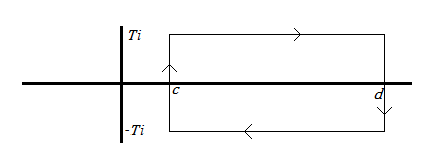
\includegraphics{analytic-chapters/dir-c1.png}
\end{figure}

Hence,
\begin{align*}
\ab{\int_{c-iT}^{c+iT}y^s\frac{ds}{s}}
&=\ab{\int_{c+iT}^{d+iT} y^s\frac{ds}{s}+\int_{d-iT}^{c-iT} y^s\frac{ds}{s}+\int_{d+iT}^{d-iT} y^s\frac{ds}{s}}\\
&\le 2\int_c^d y^{\si}\frac{d\si}{T}+\ab{\int_{d+iT}^{d-iT} y^s\frac{ds}{s}}.
\end{align*}
Note that the last integral goes to 0 as $d\to \iy$, because $|y^s|=|y^d|\to 0$. Hence, taking $d\to \iy$ gives
\[
\ab{\int_{c-iT}^{c+iT}y^s\frac{ds}{s}}
\le 2\int_c^{\iy} \frac{y^{\si}}{T}\,d\si=-\frac{2y^c}{T\ln y}=\frac{2y^c}{T|\ln y|}.
\]
This gives $\ab{\rc{2\pi i}\int_{c-iT}^{c+iT} y^s\frac{ds}{s}}\le \frac{y^c}{\pi T}{|\ln y|}$.

%Now we show the bound $\ab{\rc{2\pi i}\int_{c-iT}^{c+iT} y^s\frac{ds}{s}}\le \frac{y^c}{2}$, for any $y$.
By Cauchy's theorem applied to the smaller segment bounded by $\Re s=c$ and the circle with radius $R=\sqrt{c^2+T^2}$,  \fixme{(picture)} we have
\begin{align*}
%\int_{c-iT}^{c+iT} y^s\frac{ds}{s}+\int_C \frac{y^s}\frac{ds}{s}&=0\\
\ab{\int_{c-iT}^{c+iT} y^s\frac{ds}{s}}
&= \ab{\int_C y^s\frac{ds}{s}}\\
&\le \pi R\frac{y^{c}}{R}=\pi y^c,
\end{align*}
since $y<1$ and $\Re s>c$ on the arc. Hence $\ab{\rc{2\pi i}\int_{c-iT}^{c+iT} y^s\frac{ds}{s}}\le \frac{y^c}2$.\\

For $y>1$, take $d<0$. Note $\frac{y^s}{s}$ is analytic in the region below except for a simple pole at 0 with residue 1 (since $y^s=1$ when $s=0$). Hence by Cauchy's Theorem,
\[
\int_{c-iT}^{c+iT} y^s\frac{ds}{s}+\int_{c+iT}^{d+iT} y^s\frac{ds}{s}+\int_{d+iT}^{d-iT} y^s\frac{ds}{s}+\int_{d-iT}^{c-iT} y^s\frac{ds}{s}=2\pi i.
\]

\fixme{[INSERT PICCY]}

Then 
\begin{align*}
\ab{\int_{c-iT}^{c+iT}y^s\frac{ds}{s}-1}
&=\ab{\int_{c+iT}^{d+iT} y^s\frac{ds}{s}+\int_{d-iT}^{c-iT} y^s\frac{ds}{s}+\int_{d+iT}^{d-iT} y^s\frac{ds}{s}}\\
&\le 2\int_d^c y^{\si}\frac{d\si}{T}+\ab{\int_{d+iT}^{d-iT} y^s\frac{ds}{s}}.
\end{align*}
The last term goes to 0 as $d\to -\iy$, so the same argument applies as in the first part to show $\ab{\rc{2\pi i} \int_{c-iT}^{c+iT}y^s\frac{ds}{s}-1}\le \frac{y^c}{\pi T\ln y}$.

By Cauchy's theorem applied to the larger segment bounded by $\Re s=c$ and the circle with radius $R=\sqrt{c^2+T^2}$, \fixme{(picture)} we have
\begin{align*}
\int_{c-iT}^{c+iT} y^s\frac{ds}{s}+\int_C y^s\frac{ds}{s}&=2\pi i\\
\ab{\int_{c-iT}^{c+iT} y^s\frac{ds}{s}-1}
&\le \ab{\int_C y^s\frac{ds}{s}}\\
&\le 2\pi R\frac{y^{c}}{R}=2\pi y^c,
\end{align*}
since $y>1$ and $\Re s<c$ on the arc. Hence $\ab{\rc{2\pi i}\int_{c-iT}^{c+iT} y^s\frac{ds}{s}}\le y^c$.\\

Proof for $y=1$ omitted.
\end{proof}
\begin{cor}\llabel{sum-coeff-Dir}
The partial sum of the coefficients of a Dirichlet series is given by 
\[
\sum_{n<x} a_n+\frac{a_x}{2}(x\in \N_0)=\rc{2\pi i} \lim_{T\to \iy}\int_{c-iT}^{c+iT} x^s f(s)\frac{ds}{s}.
\]
The error from truncating the integral is
\[
\ab{\pa{\sum_{n<x} a_n+\frac{a_x}{2}(x\in \N_0)}-\pa{\rc{2\pi i} \int_{c-iT}^{c+iT} x^s f(s)\frac{ds}{s}}}\le \sum_{n=1}^{\iy} \pf xn^c a_n\min\pa{1,\rc{T\ab{\ln\pf xn}}}.
\]
\end{cor}


%%%%%%%%%%%%
\chapter{Zeta functions and the prime number theorem}\llabel{zeta-l-pnt}
\index{prime number theorem}
\section{Prime number theorem: Outline}
\begin{df}
Define the prime-counting function
\[
\pi(x)=|\set{p\le x}{p\text{ prime}}|.
\]
\end{df}
Our goal in this chapter is to prove the following famous theorem (in all its error-bounded glory).
\begin{thm}[Prime number theorem]\llabel{pnt}
There is an effective constant $C>0$ such that
\[
\pi(x)=\text{li}(x)+O(xe^{-C\sqrt{\ln x}})
\]
for all $x\ge 1$.
\end{thm}
Here $\Li(x)$ denotes the \textbf{logarithmic integral}
\[
\Li(x)=\int_2^x \frac{dt}{\ln t}.
\]
Note that $\Li(x)= \frac{x}{\ln x}+O\pf{x}{(\ln x)^2}$ as $x\to \iy$, since integration by parts gives
\begin{align}
\nonumber\li(x)&=\int_2^x \frac{dy}{\ln y} +O(1)=\frac{x}{\ln x}+\int_2^x \frac{dy}{(\ln y)^2}+O(1)\\
&=\frac{x}{\ln x}+O\pf{x}{(\ln x)^2}.\llabel{li-ibp}
\end{align}

\subsection{The big picture}

We recommend Andrew Granville's article IV.2 Analytic Number Theory in~\cite{PCTM} for an overview.

How might we guess at the asymptotics for $\pi(x)$? (In particular, why is it closer to $\Li(x)$ than $\fc{x}{\ln x}$?) By studying tables of primes up to 3 million, Gauss hypothesized that the density of primes at around $x$ is around $\rc{\ln x}$, and hence that the number of primes up to $x$ would be the integral $\Li(x)=\int_2^x \frac{dt}{\ln t}$. Making a table of $\pi(x)$ and the difference $\Li(x)-\pi(x)$, we find that the difference is slightly more than on the order of $\sqrt x$, so this seems to be a good estimate.

It is a common theme in analytic number theory to make conjectures about the distribution of primes (or other subsets of interest) by assuming they are randomly distributed according to some probability model. Often a simple model works for simple asymptotics up to $x$, and the model needs to be refined or corrected when dealing with more complicated quantities such as number of primes in a small interval, or spacing between primes.

\begin{mdl}[Gauss-Cram\'er model]
For $n\ge 3$, let $X_n$ be the random variable such that
\begin{align*}
X_n&=1 \text{ with probability }\rc{\ln n}\\
X_n&=0 \text{ with probability }1-\rc{\ln n}.
\end{align*}
Then the sequence $X_n$ behaves similarly to the sequence 
\begin{align*}
a_n&=1 \text{ if $n$ is prime}\\
a_n&=0 \text{ otherwise.}
\end{align*}
\end{mdl}
The Gauss-Cram\'er model exactly predicts $\pi(x)\sim \Li(x)$. The model gives more than just the asymptotics of $\pi(x)$, though, it can also be used to think about primes in short intervals $\pi(x+y)-\pi(x)$. \\

\prbbox{What are the shortcomings of the Gauss-Cram\'er model?}
\vskip0.15in

\subsection{Main steps}
The main steps in the proof are as follows.
\begin{enumerate}
\item When we have a Dirichlet series
\[
F(s)=\sum_{n=0}^{\iy} a_n n^{-s},
\]
we can get estimates for $\sum_{n=0}^N a_n$ by ``plucking out" those coefficients: The equation %using the Mellin transform:
\[
\rc{2\pi i}\lim_{T\to\iy}\int_{c-iT}^{c+iT} y^s\frac{ds}{s}=\begin{cases}
1,&\text{if }y>1\\
\rc 2,&\text{if }y=1\\
0,&\text{if }y<1.
\end{cases}
\]
gives
\[
\rc{2\pi i} \lim_{T\to \iy}\int_{c-iT}^{c+iT} x^s f(s)\frac{ds}{s}=\sum_{n<x} a_n+\frac{a_x}{2}(x\in \N_0).
\]
We use the more precise statement giving error bounds (Corollary~\ref{dirichlet}.\ref{sum-coeff-Dir}).

We want a Dirichlet series where the sum of the first $N$ terms is related to $\pi(N)$.
Let
\[
\ze(s)=\prod_{p\text{ prime}} \rc{1-p^{-s}}=\sum_{n=1}^{\iy}\rc{n^s}.
\]
We consider the function
\[
-\frac{\zeta'(s)}{\zeta(s)}=\sum_{p\text{ prime}} \frac{(\ln p)p^{-s}}{1-p^{-s}}
=\sum_{n=1}^{\iy} \La(n)n^{-s}.
\]
We use this function because $\psi(x):=\sum_{n<x} \La(n)$ gives information on $\pi(x)$, and 
$-\frac{\zeta'}{\zeta}$ continues into a meromorphic function on $\C$ (since $\ze$ does). We now have the estimate
\[
\psi(x)=\rc{2\pi i}\int_{c-iT}^{c+iT} -\frac{\zeta'(s)}{\zeta(s)} x^s\frac{ds}{s}+(\text{error}).
\]
\item We know $\zeta$ has analytic continuation (Theorem~\ref{zeta-continues}). Hence we can move the path of integration to $c<0$. From Cauchy's integral formula, we get extra terms from the horizontal integrals (integrals involving $-\frac{\zeta'}{\zeta}$) and terms $\frac{x^{\rho}}{\rho}$ from Cauchy's integral theorem from the zeros of $\zeta(s)$. {\it This is why we care about its zeros!} Zeros with large real part contribute large error terms.
We will need the following.
\begin{enumerate}
\item
We apply the product development (Theorem~\ref{complex-analysis}.\ref{product-development}) on $\xi(s)=\pi^{-\frac s2}\zeta(s)\Ga\pf s2$ to obtain
\[
\frac{\zeta'(s)}{\zeta(s)}=\sum_{\rh\text{ zero of }\zeta}\pa{\rc{s-\rh}+\rc{\rh}}+\cdots
\]
(Theorem~\ref{xi-product-development}).
%\[
%\frac{\ze'(s)}{\ze(s)}=\sum_{|T-\Im \rh|<1}\rc{s-\rh}+O(\ln T).
%\]
%(See Theorem~\ref{zeta-l-pnt}.\ref{zeta-product-development}).
\item
Using the above equation for $\frac{\zeta'}{\zeta}$, we calculate the asymptotics of $N(T)$, the number of zeros in $\set{\si+it}{(\si,t)\in[0,1]\times[-T,T]}$ (Theorem~\ref{zeta-zeros}).
\item
From (a) to (b) we get a zero-free region for $\ze$ (which includes $\Re s\ge 1$) (Theorems~\ref{weak-zeta-zeros} and \ref{zeta-zero-free}).
\end{enumerate}
From the zero-free region we get a bound for $\sum\frac{x^{\rh}}{\rh}$, as well as the horizontal integrals. 
If the Riemann hypothesis is true, then we can enlarge our zero-free region to $\Re s> \rc2$, which is even better. 
\item Finally we use the estimate for $\psi(x)$ to get an estimate for $\pi(x)$ (Lemma~\ref{partial-sum-pi}).
\end{enumerate}
\index{zeta function}
%\index{zeta function|Riemann}
%\index{zeta function|Hurwitz}
\section{Riemann zeta function}
\begin{df}
The \textbf{Riemann zeta function} is defined by %, the $L$-function with character $\chi$, and the \textbf{Hurwitz zeta function}, are respectively given by
%\begin{align*}
\[
\zeta(s)=\sum_{n=1}^{\iy} \rc{n^s}
%L(s,\chi)&=\sum_{n=1}^{\iy} \frac{\chi(n)}{n^s}\\
%\zeta(s,a)&=\sum_{n=0}^{\iy} \rc{(n+a)^s},&0<a\le 1.
%\end{align*}
\]
when $\Re s>1$. This will be generalized to $L$-functions $L(s,\chi)$ in Definition~\ref{l-func-dirichlet}.\ref{l-func-def}.
\end{df}
%Note that the $L$-function and $\zeta(s,a)$ are generalizations of $\zeta$ in different directions.
%Note
%\[
%L(s,\chi)=k^{-s}\sum_{r=1}^k \chi(r)\zeta\pa{s,\frac rk}.
%\]
By Theorem~\ref{euler-product} and by unique factorization in $\Z$, we can write
\[
\ze(s)=\prod_{p\text{ prime}}\rc{1-p^{-s}}.
\]
By taking the logarithmic derivative, we have %(VALID BY...), we have
\[
-\frac{\zeta'(s)}{\zeta(s)}=\sum_p \frac{d}{ds}\ln(1-p^{-s})
=\sum_p (\ln p)\frac{p^{-s}}{1-p^{-s}}=\sum_p \ln p\sum_{k=1}^{\iy} p^{-ks}.
\]
Interchanging order of summation gives
\begin{equation}\llabel{log-diff-zeta}
-\frac{\zeta'(s)}{\zeta(s)}=\sum_{n=1}^{\iy} \La(n)n^{-s}, \quad \Re s>1,
\end{equation}
where the von Mangoldt function $\La(n)$ is defined as
\[
\La(n)=\begin{cases}
\ln p,&n=p^r,\,p\text{ prime, }r\in \N.\\
0,&\text{else}
\end{cases}
\]

The most important property of $\ze$ is its analytic continuation and functional equation.
\begin{thm}\llabel{zeta-continues}
$\zeta(s)$ can be analytically continued to a meromorphic function with a simple pole at $s=0,1$. %with residue 1. 
It satisfies the functional equation
\[
\zeta(s)=2(2\pi)^{s-1}\Ga(1-s)\sin\pf{\pi s}2 \zeta(1-s).
\]
Letting $\xi(s)=\pi^{-\frac s2}\zeta(s)\Ga\pf s2$, we have\footnote{The factor $\Ga\pf s2$ can be thought of as coming from the infinite place---see Chapter~\ref{l-nf}.}
\[
\xi(s)=\xi(1-s).
\]
Moreover, $\ze(s)$ has zeros $-2\N$ (the trivial zeros); all other zeros are in the critical strip $0\le \Re s\le 1$.
\end{thm}
To prove this, we first need the transformation law for the theta function; we will show the functional equation for $\ze$ by writing it in terms of $\te$. As we will prove a more generalized transformation law, we will postpone the proof for $\te$.
\begin{df}
Define the \textbf{theta function} by
\[
\te(u)=\sum_{n\in \Z}e^{-\pi n^2u},\quad \Re u>0.
\]
\end{df}
\begin{pr}[Transformation law for $\te$]\llabel{theta-law}
For all $u$ with $\Re u>0$,
\[
\te\prc u = u^{\rc2} \te(u).
\]
\end{pr}
This is a special case of Proposition~\ref{l-func-dirichlet}.\ref{theta-transforms}.
\begin{proof}[Proof of Theorem~\ref{zeta-continues}]
We first analytically continue $\zeta$ to $\Re s>0$, show the functional equation is true for $0<\Re s<1$, and use it to establish analytic continuation to $\C$.

Note
\begin{equation}\llabel{continue-zeta-to-0}
\zeta(s)=\rc{s-1}+\sum_{n=1}^{\iy}\ba{
n^{-s}-\int_n^{n+1} x^{-s} \,dx
}
=\rc{s-1}+\sum_{n=1}^{\iy} \int_n^{n+1} (n^{-s}-x^{-s})\,dx
\end{equation}
Since for $n\le x\le n+1$ we have
\begin{align}
\nonumber|n^{-s}-x^{-s}|&=\ab{\int_{n}^x sx^{-s-1}\,dx}
\le|s|n^{-s-1}\\
\llabel{bound-zeta-summands}
\ab{\int_n^{n+1} n^{-s}-x^{-s}\,dx}&\le |s|n^{-s-1},
\end{align}
the sum~(\ref{continue-zeta-to-0}) converges uniformly locally for $\Re s>0$ and extends $\zeta$ to an analytic function for $\Re s>0$.

We claim that
\begin{equation}\llabel{zeta-theta}
2\xi(s)=\int_0^{\iy} (\theta(u)-1)u^{\frac s2} \frac{du}{u},\quad \Re s>1
\end{equation}
%i.e. $\zeta(-2s)$ is the Mellin transform of $\frac{\theta(u)-1}2$.
Indeed, we have
\begin{align*}
\int_0^{\iy} (\theta(u)-1)u^{\frac s2} \,\frac{du}u
&=\int_0^{\iy} 2\sum_{n=1}^{\iy} e^{-\pi n^2u}u^{\frac s2}\frac{du}u\\
&=2\sum_{n=1}^{\iy} \int_0^{\iy} e^{-\pi n^2u}u^{\frac{s}2}\,\frac{du}u\\%absolute convergence?
&=2\sum_{n=1}^{\iy} \int_0^{\iy} e^{-u} \pf{u}{\pi n^2}^{\frac s2}\,\frac{du}u&u\mapsfrom \frac{u}{\pi n^2}\\
&=2\pi^{-\frac s2}\pa{\sum_{n=1}^{\iy} \rc{n^s}}\pa{\int_0^{\iy} e^{-u} u^{\frac s2}\,\frac{du}u}\\
&=2\pi^{-\frac s2} \zeta(s)\Ga\pf{s}2=2\xi(s).
\end{align*}
The theta transformation law~\ref{theta-law} give that for $\Re s>1$,
\begin{align*}
2\xi(s)&=\int_0^1 (\theta(u)-1)u^{\frac s2}\frac{du}u
+\int_1^{\iy} (\theta(u)-1)u^{\frac s2} \frac{du}{u}\\
&=%-\frac{2}{s}+
\int_1^{\iy} \pa{\theta\prc u-1}u^{\frac s2} \frac{du}u +\int_1^{\iy} (\theta(u)-1)u^{\frac s2}\frac{du}u&u\mapsfrom \rc u\\
&=\int_1^{\iy}\pa{u^{-\rc2}\te\prc u-1} u^{\frac{1-s}2}\frac{du}u+\int_1^{\iy}(u^{\fc{1-s}2}-u^{-\fc{s}2})\fc{du}u
+\int_1^{\iy} (\theta(u)-1)u^{\frac s2}\frac{du}u\\
&=-\frac{2}{s}-\frac{2}{1-s}+\int_1^{\iy} (\theta(u)-1)u^{\frac{1-s}2}\frac{du}u+\int_1^{\iy}(\te(u)-1) u^{\frac s2}\frac{du}u.
\end{align*}
The last expression converges for all $\Re s>0$, so in fact equals $2\ze(s)$ for all $\Re s>0$ by uniqueness of analytic continuation. Since the last expression is symmetric under $1-s\mapsto s$, the functional equation for $\xi$ follows.

%To get the functional equation for $\ze$, note
The functional equation for $\xi$ gives
\begin{align*}
\ze(s)&=\pi^{\fc s2} \Ga\pf s2^{-1}\pi^{-\fc{1-s}2} \Ga\pf{1-s}2\ze(1-s)\\
&=\pi^{s-\rc2} \frac{\Ga\pf{1-s}2}{\Ga\pf{s}2}\ze(1-s)\\
&=\pi^{s-\rc2}\Ga\pf{1-s}2 \Ga\pa{1-\fc s2} \frac{\sin\pf{\pi s}2}{\pi}\ze(1-s)&\text{by Proposition~\ref{complex-analysis}.\ref{gamma-facts}(5)}\\
&=2(2\pi)^{s-1}\sin\pf{\pi s}2\Ga(1-s)\ze(1-s)&\text{by Proposition~\ref{complex-analysis}.\ref{gamma-facts}(6)}
\end{align*}

Finally, the statement about zeros follows from the fact that $\ze$ has no zeros with $\Re s>1$ (as $\fc{\ze'}{\ze}$ is holomorphic there) and the functional equation, noting $\sin\pf{\pi s}{2}=0$ exactly when $s$ is an even integer, with the zero at $s=0$ cancelled by the pole at 1 of $\ze$.
\end{proof}
\begin{thm}[Product development of $\xi$]\llabel{xi-product-development}
The function $(s^2-s)\xi(s)$ is entire of order 1, and $\xi(s)$ has the product expansion
\[
\xi(s)=\frac{e^{A+Bs}}{s^2-s}\prod_{\rho\text{ zero of }\ze} \pa{1-\frac s{\rh}}e^{\frac s{\rh}}.
\]
Then $\frac{\zeta'}{\zeta}(s)$ has the partial-fraction expansion
\[
\frac{\zeta'}{\zeta}(s)=B-\rc{s-1}+\rc{2}\ln(\pi) -\rc2\frac{\Ga'}{\Ga}\pa{\frac s2+1}+\sum_{\rh\text{ nontrivial zero of }\zeta}\pa{\rc{s-\rh}+\rc{\rh}}.
\]
\end{thm}
From now on, unless otherwise specified, when we say zero of $\ze$ we mean {\it nontrivial} zero.
\begin{proof}
Note $(s^2-s)\xi(s)$ is entire because $\xi$ only has 2 simple poles at $0,1$. To show it has order 1 we need two inequalities.\\

\noindent \underline{Step 1:} There is no constant $C$ so that $(s^2-s)\xi(s)\precsim e^{C|s|}$: Indeed, for real $s$ and any constant $C$, by Stirling's approximation~\ref{complex-analysis}.\ref{stirling} we have
\begin{align*}
(s^2-s)\xi(s)&=(s^2-s)\pi^{-\frac s2}\Ga\pf s2\ze(s)\\
&\succsim s^{-\rc 2}\pf{s}{2e\pi}^{\frac s2}
\succsim e^{Cs}.
\end{align*}
\noindent\underline{Step 2:} There is a constant $C$ so that $(s^2-s)\xi(s)\precsim e^{C|s|\ln|s|}$: $e^{|s|\ln|s|}\ge1$ for all $s$ so it suffices to prove this for sufficiently large $s$. By the integral and sum formulas for $\Ga$ and $\xi$, and the fact that $|x^s|=|x^{\Re s}|$, we have
\[
|\xi(\si+ti)|\le \pi^{-\frac{\si}{2}}\Ga\pf{\si}{2}\ze(\si),\quad \si>1.
\]
By symmetry of $\xi$ is suffices to consider $\si\ge \rc2$. (``Nudging" $|s|$ in $e^{C|s|\ln|s|}$ by a constant changes it by at most a constant factor.)
Consider 2 cases.
\begin{enumerate}
\item
$\si>2$: Then $\pi^{-\frac{\si}{2}}<1$ and $\ze(\si)<\ze(2)$ so by Stirling's approximation~\ref{complex-analysis}.\ref{stirling},
\[
|\xi(\si+ti)|\precsim
\Ga\pf{\si}2
%\precsim %\pf{\si}{2}^{\frac{\si}2-\rc 2}e^{-\frac{\si}{2}}
=e^{|(\ln\Ga)(\si)|}=e^{\pa{\frac{\si}2-1}\ln\frac{\si}2-\frac{\si}2+O(1)}
\]
from which the result follows.
\item
$\frac12\le \si\le 2$: From~(\ref{bound-zeta-summands}), we have for $s$ bounded away from 1,
\[
\zeta(s)\le O(1)+|s| \sum_{n=1}^{\iy} n^{-\frac 32}=O(|s|).
\]
This time $\Ga\pf{\si}{2}=O(1)$ so
\[
|(s^2-s)\xi(s)|\le \ab{
s^2\pi^{-\frac{\si}2}\zeta(s)\Ga\pf{\si}2}
=O(|s|^3)\precsim e^{C|s|\ln|s|}.
\]
\end{enumerate}
This shows $(s^2-s)\xi(s)$ has order 1.\\

\noindent\underline{Step 3:} By the product development~\ref{complex-analysis}.\ref{product-development}, noting the the zeros of $(s^2-s)\xi$ are the nontrivial zeros of $\ze$ (since $\Ga$ has no zeros and trivial zeros of $\ze$ come from the poles of $\Ga$ in the definition of $\xi$), we get
\[
(s^2-s)\xi(s)=e^{A+Bs}\prod_{\rh\text{ zero of }\zeta}\pa{1-\frac{s}{\rh}}e^{\frac s{\rh}}.
\]
Dividing by $s^2-s$ and log-differentiating gives
\[
\frac{\xi'}{\xi}(s)=B-\rc{s}-\rc{s-1}+\sum_{\rh} \pa{\rc{s-\rh}+\rc{\rh}}.
\]
Since $\ze(s)=\pi^{\frac s2}\Ga\pf{s}2^{-1}\xi(s)$, we get
\begin{align*}
\frac{\ze'}{\ze}(s)&=\rc{2}\ln\pi +\rc2\frac{\Ga'}{\Ga}\pa{\fc s2}+B-\rc{s}-\rc{s-1}+\sum_{\rh} \pa{\rc{s-\rh}+\rc{\rh}}\\
&=\rc{2}\ln\pi +\rc2\frac{\Ga'}{\Ga}\pa{\fc s2+1}+B-\rc{s-1}+\sum_{\rh} \pa{\rc{s-\rh}+\rc{\rh}},&\Ga(z)=\fc{\Ga(z+1)}{z}.\qedhere
\end{align*}
\end{proof}
\section{Zeros of zeta}
Note that from the function equation, $\ze(s)$ has simple zeros at $-2\N$. We call these trivial zeros. More importantly for us are the zeros with real part in $[0,1]$.

Denote by $N(T)$ be the number of zeros of $\zeta$ in $\set{\si+it}{(\si,t)\in [0,1]\times [-T,T]}$, counting multiplicity. We first give asymptotics on the vertical distribution of zeros of $\zeta$ (von Mangoldt's formula, Theorem~\ref{zeta-zeros}), then give a zero-free region for $\zeta$ (Theorem~\ref{zeta-zero-free}).
\begin{lem}\llabel{weak-zeta-zeros}
Define $\cal L(t)=\ln (|t|+2)$. 
For $s=\si+it$ with $\si\in [-1,2]$, we have\footnote{Note $\rc{s-1}=O(1)$ when $s$ is bounded away from 1.}
\begin{align}
\llabel{weak-zeta-zeros-eq1}
\frac{\zeta'(s)}{\zeta(s)}
&={\color{gray}-\rc{s-1}}
+\sum_{\rh}\pa{\rc{s-\rh}+\rc{\rh}}+O(\cal L)\\
\nonumber
&={\color{gray}-\rc{s-1}}
+\sum_{|\Im(s-\rh)|<1} \rc{s-\rh} +O(\cal L).
\end{align}
Moreover, there are $O(\cal L)$ zeros $\rh$ with $|\Im(s-\rh)|<1$, i.e. the number of zeros with imaginary part in $[t,t+1]$ is $O(\ln t)$, as $t\to \iy$.
\end{lem}
Note this gives $N(T)=O(T\ln T)$. The next theorem will give an improvement of this estimate.
\begin{proof}
Our strategy is this: at a point where we know $\frac{\ze'}{\ze}$ is bounded ($s=2+it$), we use Theorem~\ref{xi-product-development} to get information on how many zeros of $\zeta$ can be close to $s$. Then we use compare $\frac{\ze'}{\ze}(\si+it)$ with $\frac{\ze'}{\ze}(2+it)$ to get the general estimate.\\

\noindent\underline{Step 1:}
Theorem~\ref{xi-product-development} gives us
\begin{equation}\llabel{zeta2-zero-sum}
\frac{\zeta'(s)}{\zeta(s)}=-\rc{s-1}+
\underbrace{B+\rc2\ln\pi}_{O(1)}
-
\rc2\underbrace{\frac{\Ga'}{\Ga}\pa{%\frac{\si}2+1+i\frac t2}
\frac s2+1}}_{(A)}+
\underbrace{\sum_{\rh} \pa{\rc{%\si+it
s-\rh}+\rc{\rh}}}_{(B)}.
\end{equation}
From Stirling's approximation~\ref{complex-analysis}.\ref{stirling}, (A) equals
\begin{equation}\llabel{gamma2-estimate}
%\underbrace{
\ln\ab{\frac{\si}{2}+1+i\frac t2}%}_{O(1+\ln |t|)}
+O(1)=
%\underbrace{\frac{1}{2\ab{\frac{\si}{2}+1+i\frac t2}}}_{O(1)}
%+O\pa{\ab{\frac{\si}{2}+1+i\frac t2}^{-2}}=
%O(\ln |t|).
O(\cal L)
\end{equation}
These two equations show~(\ref{weak-zeta-zeros-eq1}).

Now suppose $s=2+it$. %Theorem~\ref{xi-product-development} says
Note that
\[
\ab{\frac{\ze'(2+it)}{\ze(2+it)}}
=\ab{\sum_{n=1}^{\iy} \La(n)n^{-2-it}}
\le \ab{\sum_{n=1}^{\iy} (\ln n)n^{-2}}<\iy,
\]
so the LHS of~(\ref{zeta2-zero-sum}) is $O(1)$.
%%%%%%
%Now we estimate (B) by truncating the sum.
Hence~(\ref{zeta2-zero-sum}) becomes
\begin{equation}\llabel{zeta2-zero-sum2}
O(\cal L)=\sum_{\rh} \pa{\rc{%\si+it
s-\rh}+\rc{\rh}}.
\end{equation}
%Note
%\[
%\Re\pa{\rc{2+it-\rh}+\rc{\rh}}=\Re\pa{
%\frac{(2+\Re \rh)-(t-\Im \rh)i}{(2-\Re \rh)^2+(t-\Im\rh)^2}
%}
%\ge\rc{4+(t-\Im \rh)^2}
%\]
%since $0\le \Re \rh\le 1$.
We estimate the terms with $|\Im(s-\rh)|<1$ by a constant to show that there aren't too many of them.
From~(\ref{zeta2-zero-sum2}) and~(\ref{gamma2-estimate}),
\begin{align}
%O(\ln |t|) &\ge \Re\sum_{|\Im(s-\rh)|<1}\pa{\rc{2+it-\rh}+\rc{\rh}}\\
%%&\ge \Re\sum_{
%%%{\footnotesize\begin{array}{c}
%%%\rh\text{ zero}\\
%%|\Im(s-\rh)|<1%\end{array}}}
%%}\frac{(2+\Re \rh)-(t-\Im \rh)i}{(2-\Re \rh)^2+(t-\Im\rh)^2}\\
%&=\sum_{|\Im(s-\rh)|<1}\rc{4+(t-\Im \rh)^2}\\
%&\ge \rc 5 |\set{\rh}{|\Im(s-\rh)|<1}|.
%
\nonumber
O(\cal L) &= \Re\sum_{\rh}\pa{\rc{2+it-\rh}+\rc{\rh}}\\
\nonumber
&\ge
\Re\sum_{\rh}\pa{
\frac{(2-\Re \rh)-(t-\Im \rh)i}{(2-\Re \rh)^2+(t-\Im\rh)^2}
}&\text{since }\Re \prc{\rh}>0\\
\nonumber
&\ge\sum_{\rh} \rc{4+(t-\Im \rh)^2}&\text{since $0\le \Re \rh\le 1$}\\
\llabel{zero-olnt}
&\ge \rc 5 |\set{\rh}{|\Im(s-\rh)|<1}|+\rc5 \sum_{|\Im(s-\rh)|\ge 1}\rc{(t-\Im \rh)^2}.
\end{align}
This proves the second part of the lemma.\\
%%We similarly consider the sum for $|\Im(s-\rh)|>1$:
%%\begin{align}
%%\llabel{olntge}
%%O(\ln|t|)
%%&\ge\sum_{|\Im(s-\rh)|\ge 1}\pa{\rc{2+it-\rh}+\rc{\rh}}\\
%%\nonumber&=\sum_{|\Im(s-\rh)|<1}\rc{4+(t-\Im \rh)^2}\\
%%\nonumber&\ge \rc5 \sum_{|\Im(s-\rh)|<1}\rc{(t-\Im \rh)^2}
%%\end{align}
%Now from~(\ref{zeta2-zero-sum}),
%\begin{align*}
%\ab{\frac{\zeta'(2+it)}{\zeta(2+it)}}
%%O(\ln|t|)
%&=\sum_{|\Im(s-\rh)|<1}\rc{s-\rh}+
%\underbrace{\sum_{|\Im(s-\rh)|<1}\rc{\rh}}_{O(\ln|t|)}
%+
%\underbrace{\sum_{|\Im(s-\rh)|\ge 1}\pa{\rc{2+it-\rh}+\rc{\rh}}}_{O(\ln|t|)}
%%&=O(\ln|t|)+\sum_{|\Im(s-\rh)|<1}\rc{s-\rh}+O(\ln|t|)+O(\ln|t|),
%\end{align*}
%as needed. (The first $O(\ln|t|)$ is because there are $O(\ln|t|)$ terms in the sum and each is at most 1 in absolute value.)\\

\noindent\underline{Step 2:} Now we consider general $s=\si+it$, by comparing it to $2+it$. We have by~(\ref{zeta2-zero-sum}) and~(\ref{gamma2-estimate}) that
\begin{align*}
&\quad \frac{\zeta'}{\zeta}(s)-\underbrace{\frac{\ze'}{\ze}(2+it)}_{O(1)}\\
&=-\rc{s-1}+O(1)+\underbrace{\rc2\pa{\ln\ab{\frac{\si}2+1+\frac t2i}-
\ln\ab{2+\frac t2i}}}_{O(1)}+\sum_{\rh} \pa{\rc{s-\rh}-\rc{2+it-\rh}}\\
&=-\rc{s-1}+O(1)+
\sum_{|\Im(s-\rh)|<1}\rc{s-\rh}-\underbrace{\sum_{|\Im(s-\rh)|<1}\rc{2+it-\rh}}_{O(\cal L)}+
\underbrace{\sum_{|\Im(s-\rh)|\ge1}\frac{(2-\si)}{(s-\rh)(2+it-\rh)}}_{O(\cal L)}.
\end{align*}
The first $O(\cal L)$ is because there are at most $O(\cal L)$ terms and each term is at most 1 in absolute value; the second is from
\[
\sum_{|\Im(s-\rh)|\ge1}\frac{2-\si}{(s-\rh)(2+it-\rh)}=O\pa{\sum_{|\Im(s-\rh)|\ge1}\frac{1}{\Im(s-\rh)^2}}=O(\cal L);
\]
the first equality is from $2-\si=O(1)$ and $\Im(s-\rh)=\Im(2+it-\rh)$; the second is by~(\ref{zero-olnt}).
\end{proof}
\index{von Mangoldt's Theorem}
\begin{thm}[von Mangoldt]\llabel{zeta-zeros}($*$) 
As $T\to \iy$,
\[
N(T)=\frac{T}{\pi}\ln\pf{T}{2\pi}-\frac{T}{\pi}+O(\ln T).
\]
\end{thm}
\begin{proof}
As $\zeta$ has only a countable number of zeros, we may assume $T$ is not the imaginary part of any zero.

Let
\[
\cal R=\set{\si+it}{(s,t)\in [-1,2]\times [-T,T]}
\]
and let $C$ be the boundary of $\cal R$. \fixme{(PICTURE)}
%Since $\Ga(\ol s)=\ol{\Ga(s)}$, the zeros of $\Ga$ are symmetric across the real axis. 
From $\xi(s)=\pi^{-\frac s2}\zeta(s)\Ga\pf s2$, we see that $\xi$ has the same zeros as $\zeta$ in this region, and simple poles at $0$ and $1$. %Now $\Ga$ has $2N(T)$ zeros (note it has no zeros on the real axis)
%and $2$ poles in $\cal R$, namely $0$ and $1$. 
Hence by Cauchy's residue formula~\ref{complex-analysis}.\ref{residue},
\[
\rc{2\pi i}\oint_{C} \frac{\xi'(s)}{\xi(s)} ds=2N(T)-2.
\]
Noting that $\xi(\ol{s})=\ol{\xi(s)}$ and $\xi(s)=\xi(1-s)$, changes of variable show that the integral on each of the sections of $C$ between $2$, $\rc 2+iT$, $-1$, and $\rc 2-iT$ are the same.\footnote{We used $\xi$ because its symmetry allows us to do this.} Let $C'$ be the part from $1$ to $\rc 2+iT$. Thus 
%(using $\pa{\prod_{k=1}^n f_k}'=\sum_{k=1}^n \frac{f_k'}{f_k}$), 
the above equals
\begin{align*}
\frac2{\pi i}\int_{C'} \frac{\xi'(s)}{\xi(s)} ds
&=\frac2{\pi i}
\int_{C'} -\frac{\ln \pi}{2}+\frac{\zeta'(s)}{\zeta(s)}+\frac{\pa{\Ga\pf{s}{2}}'}{\Ga\pf s2}\,ds&\frac{\pa{\prod_{k=1}^n f_k}'}{\prod_{k=1}^n f_k}=\sum_{k=1}^n \frac{f_k'}{f_k}\\
&=\frac2{\pi}\Im
\int_{C'} -\frac{\ln \pi}{2}+\frac{\zeta'(s)}{\zeta(s)}+\frac{\pa{\Ga\pf{s}{2}}'}{\Ga\pf s2}\,ds
&\text{(expression is real)}.
\end{align*}
We break this up into 3 integrals and estimate each part separately.
\begin{enumerate}
\item $\Im\int_{C'}-\frac{\ln \pi}{2}\,ds=-\frac{T}{2}\ln \pi$.
\item Using the estimate for $\frac{\zeta'}{\zeta}$ in Lemma~\ref{weak-zeta-zeros},  we evaluate the second integral. Note that $\ln\zeta$ is defined for $\Re s> 1$ and is uniformly bounded for $\Re s=2$:
\begin{align*}
(\ln\zeta)(s)&=\sum_{p\text{ prime}} \ln(1-p^{-s}) \\
|(\ln\zeta)(2+it)|&\le\sum_{p\text{ prime}} 2p^{-2}.
\end{align*}
(Just bound $\ln$ linearly near 1, or expand in Taylor series.)  
Note $\ln(x-\rh)$ is well-defined on $C'$ for any $\rh$. Hence by Theorem~\ref{weak-zeta-zeros},
\begin{align*}
\Im\int_{C'}\frac{\zeta'}{\zeta}(s)\,ds
&=(\Im(\ln\zeta)(2+iT)-{\Im(\ln\zeta)(2)})+\int_{2+iT}^{\rc 2+iT} \frac{\zeta'}{\zeta}(s)\,ds\\
&=O(1)+\int_{2+iT}^{\rc 2+iT} \Im\pa{\sum_{|\Im(s-\rh)|<1}\rc{s-\rh}}+O(\ln T)\,ds\\
&=O(\ln T)+\sum_{|\Im(s-\rh)|<1}\Im(\ln(x-\rh))|^{\rc2+Ti}_{2+Ti}\\
&\le O(\ln T)+2\pi O(\ln T)
\end{align*}
since there are at most $\ln T$ terms in the sum.
\item We estimate the last integral using Stirling's formula~\ref{complex-analysis}.\ref{stirling}. (Note that $\ln\Ga$ is well-defined for $s\in C'$.)
\begin{align*}
\int_{C'}\frac{\pa{\Ga\pf s2}'}{\Ga\pf s2}
&=\ba{\Im(\ln\Ga)\pf s2}^{\rc 2+Ti}_2\\
&=\Im(\ln \Ga)\pa{\frac 14+\frac{T}{2}i}\\
&=\Im\ba{\pa{-\rc 4+\frac T2i}\ln\pa{\rc 4+\frac T2i}-\pa{\rc 4+\frac T2i}+O(1)}\\%&\text{by Theorem~\ref{complex-analysis}.\ref{stirling}}\\
&=\frac T2\ln\pf T2-\frac T2+O(1).&\qedhere
\end{align*}
\end{enumerate}
Now put everything together to get
\begin{align*}
N(T)-2&=\frac{2}{\pi}\pa{-\frac T2\ln \pi+O(\ln T)+\pa{\frac T2\ln\pf T2-\frac T2+O(1)}}\\
N(T)&=\frac{T}{\pi}\ln\pf{T}{2\pi}-\frac{T}{\pi}+O(\ln T).
\end{align*}
\end{proof}
\begin{thm}[Zero-free region for $\zeta$]\llabel{zeta-zero-free}
There are no zeros of $\zeta$ with $\Re s\ge 1$. Moreover, there is a constant $c>0$ such that for $|t|>2$, every zero $\si+it$ satisfies
\[
\si<1-\frac{c}{\ln|t|}.
\]
\end{thm}
\fixme{PICTURE!}
\begin{proof}
%(The proof of the first statement will give us motivation for the second.)
%We know that $\frac{\zeta'}{\zeta}$ has no pole for $\Re s>1$, and hence $\zeta$ has no zero for $\Re s>1$. Thus for the first part it suffices to prove that no zero has real part 1.
We already noted $\ze$ has no zero for $\Re s>1$ (Theorem~\ref{zeta-continues}), so for the first part it suffices to prove that no zero has real part 1.

If $\zeta$ had a zero $1+it$, then $\frac{\zeta'}{\zeta}$ would have a pole of positive residue at $1+it$. For $s=\si+it$, $\si>1$ we have $-\frac{\zeta'}{\zeta}(s)=\sum_{n=1}^{\iy} \frac{\La(n)}{n^s}$, so this means that as $\si\to 1^+$,
many of the important terms would have $n^{-it}$ ``close" to $-1$, to make it blow up in the negative direction. For those terms, we have $n^{-2it}$ ``close" to $1$. This would force $-\frac{\zeta'}{\zeta}(\si+2ti)$ to have a pole of positive residue at $1+2ti$, i.e $\zeta$ to have a pole at $1+2ti$, contradicting the fact that it is analytic there.

We now make this idea precise. What we want is an inequality between some function of an angle and its double, so that if one is small it forces the other to be large. So we consider
\[
0\le 2(1+\cos\theta)^2=3+4\cos \theta +\cos 2\theta.
\]
This gives
\[
0\le 3+4\Re(n^{-it})+\Re(n^{-2it}).
\]
Multiplying by $\La(n)n^{-\si}$ and summing, we get
\begin{equation}\llabel{zero-free-zeta-inequality}
0\le 3\pa{-\frac{\ze'}{\ze}(\si)} 
+4\Re\pa{-\frac{\ze'}{\ze}(\si+ti)}
+\Re\pa{-\frac{\ze'}{\ze}(\si+2ti)},\quad\si>1.
\end{equation}
Letting $r$ be the degree of the zero at $1+ti$, we have by Lemma~\ref{weak-zeta-zeros}
\[
0\le\pa{\frac{3}{\si-1}+O(1)}
-\pa{\frac{4r}{\si-1}+O(\cal L)}
+\Re\pa{-\frac{\ze'}{\ze}(\si+2ti)}\text{ as }\si\to 1^+.
\]
If $r\ge 1$, then this gives $-\frac{\ze'}{\ze}(\si+2ti)\to \iy$ as $\si\to 1^+$, contradiction. Hence $r=0$; $1+it$ is not a zero.

For the second statement, we have to use the partial fraction decomposition~\ref{xi-product-development}.
Suppose $\rh=(1-\de)+it$ is a zero. By Lemma~\ref{weak-zeta-zeros}, we have
\[
-\frac{\zeta'(s)}{\zeta(s)} = O(\ln|t|) -\sum_{\rh}\pa{\rc{s-\rh}+\rc{\rh}}\le O(\ln|t|)-\rc{s-\rh}.
\]
%(All terms in the last sum are positive.)
Then
\begin{align*}
-\Re\frac{\zeta'}{\ze}(\si+ti)&\le O(\ln|t|)-\frac{1}{\si+\de-1}\\
-\Re\frac{\zeta'}{\ze}(\si+2ti)&\le O(\ln|2t|)=O(\ln |t|).
\end{align*}
For $\si>1$, plugging this into~(\ref{zero-free-zeta-inequality}) gives
\begin{align*}
0&\le \frac{3}{\si-1}+O(\ln|t|)-\frac{4}{\si+\de-1}\\
\implies \frac{4}{\si+\de-1}&<\frac{3}{\si-1}+C_1\ln|t|
\end{align*}
for some $C_1$.
Now take $\si=1+4\de$ to get
\[
\frac{4}{5\de}<\frac{3}{4\de}+C_1\ln|t|,
\]
giving
\[
\de>\frac{1}{20C_1\ln|t|}
\]
as needed.
\end{proof}
\section{Prime number theorem: proof}
Now we gather everything together to prove the prime number theorem. We first show the following.
\index{von Mangoldt's formula}
\begin{thm}[von Mangoldt's formula]\llabel{von-Mangoldt-formula}
For an integer $x>2$ and $x\ge T$,
\begin{equation}\llabel{v-M-f}
\psi(x)= x-\sum_{|\Im(\rh)|<T}\frac{x^{\rh}}{\rh}
+O\pa{
\frac{x(\ln x)^2}{T}%+
%\frac{x(\ln T)^2}{T}+\ln x
}.
\end{equation}
\end{thm}
\begin{proof}
\noindent{\underline{Step 1:}} We estimate $\psi(x)$ using Theorem~\ref{dirichlet}.\ref{sum-coeff-Dir}. Suppose $x$ is an integer; the theorem gives
\begin{align*}
\ab{\psi(x)-\pa{
\int_{c-iT}^{c+iT} x^s\pa{-\fc{\ze'}{\ze}(s)\frac{ds}s
}}}&\le
\La(x)+
\sum_{n\ge 1,\,n\ne x} \pf xn^c\La(n)\rc{T\ab{\ln\pf xn}}\\
&\le 
\ln(x)+\sum_{n\ge 1,\,n\ne x}\pf xn^c\fc{\ln(n)}{T\ab{\ln\pf xn}}.
\end{align*}
%Assume $x$ is a large integer (i.e. bounded away from 1) and 
Take
\[
c=1+\rc{\ln x}.
\]
Note that this makes $x^c=ex=O(x)$. 
To estimate the sum we split it into several parts.
\begin{enumerate}
\item
$1\le n< \frac{x}{e}$: We have
\begin{align*}
\sum_{1\le n<\frac xe} \pf xn^c \frac{\ln n}{T\ab{\ln\pf xn}}
&\precsim \frac{x\ln x}{T}\sum_{1\le n<x}\rc{n}\\
&\sim \frac{x(\ln x)^2}{T}.
\end{align*}
\item
$\frac xe\le n< ex$: We have
\begin{align*}
\sum_{\frac xe\le n<ex,\,n\ne x}\pf xn^c \ln n\frac{1}{T\ab{\ln\pf xn}}
&\precsim \sum_{\frac xe\le n<ex,\,n\ne x} \cancel{e^{1+\rc{\ln x}}} \frac{\ln n}{T\ab{\ln\pf xn}}\\
&\precsim \rc{T}\sum_{\frac xe\le n<ex,\,n\ne x}\frac{\ln x}{\ab{1-\frac xn}}&\text{ using $\ln x\sim x-1$ when $x\approx 1$}\\
&\precsim \frac{x\ln x}{T}\sum_{\frac xe\le n<ex,n\ne x}\frac{1}{|n-x|}\\
&\precsim\frac{x\ln x}{T}\sum_{1\le n< (e-1)x}\frac{1}{n}\\
&\sim\frac{x(\ln x)^2}{T}.
\end{align*}
\item $n\ge ex$: We have
\begin{align*}
\sum_{n\ge ex} \pf xn^c \frac{\ln n}{T}&<\frac{x}{T}\int_{ex-1}^{\iy} \frac{\ln y}{y^c}\,dy&\frac{\ln y}{y^c}\text{ decreasing for }y>e\\
&=\frac xT\ba{\frac{-y^{-c+1}\ln y}{c-1}-\frac{y^{-c+1}}{(c-1)^2}}^{\iy}_{ex-1}\\
&\sim \frac{x(\ln x)^2}{T}.
\end{align*}
\end{enumerate}
Putting everything together gives
\begin{equation}\llabel{von-M-1}
\ab{\psi(x)-\pa{
\int_{c-iT}^{c+iT} x^s\pa{-\fc{\ze'}{\ze}(s)}\frac{ds}s
}}=O\pa{\frac{x(\ln x)^2}{T}+\ln x}.
\end{equation}

\noindent\underline{Step 2:} We move the line of integration to $\Re s=-1$. Assuming that $T$ is not the imaginary part of any root, by Cauchy's residue theorem~\ref{residue} \fixme{PICTURE}
\[
\int_{c-iT}^{c+iT} \frac{x^s}{s}\frac{\zeta'}{\ze}(s)\,ds
+\underbrace{\int_{c+iT}^{-1+iT} \frac{x^s}{s}\frac{\zeta'}{\ze}(s)\,ds}_{I_{h,1}}
+\underbrace{\int_{-1+iT}^{-1-iT} \frac{x^s}{s}\frac{\zeta'}{\ze}(s)\,ds}_{I_{v}}
+\underbrace{\int_{-1-iT}^{c-iT} \frac{x^s}{s}\frac{\zeta'}{\ze}(s)\,ds}_{I_{h,2}}
=\fc{\ze'}{\ze}(0)-x+\sum_{|\Im\rh|<T}\frac{x^{\rh}}{\rh}.
\]
Here $\fc{x^{\rh}}{\rh}$ are the resuides at the zeros, $-x$ comes from the pole of $\ze$ at 1, and $\fc{\ze'}{\ze}(0)$ comes from the pole of $\rc s$.
Then
\begin{equation}\llabel{von-M-2}
\int_{c-iT}^{c+iT} \frac{x^s}{s}\pa{-\fc{\zeta'}{\ze}(s)}\,ds-x=1+I_{h,1}+I_{h,2}+I_v-\sum_{\Im\rh<T}\frac{x^{\rh}}{\rh}.
\end{equation}
We estimate each summand.
\begin{enumerate}
\item For the horizontal integrals, we use the estimate~\ref{weak-zeta-zeros} to get
\begin{align*}
\ab{\frac{\ze'}{\ze}(s)}&=\ab{\sum_{|\Im(s-\rh)|<1} \rc{s-\rh}}+O(\ln T),\quad s=\si+Ti\\
&\le \sum_{|\Im(s-\rh)|<1}\rc{\Im(s-\rh)}+O(\ln T).
\end{align*}
We would like to bound $\Im(s-\rh)$ away from 0. To do this, note that there are $O(\ln T)$ roots in with $\Im \rh\in [T,T+1]$ by Lemma~\ref{weak-zeta-zeros}. Hence by tweaking $T$ slightly\footnote{Changing $T$ by a constant does not change the error term of~(\ref{v-M-f}); moreover the change in the LHS sum is $O\pa{\fc xT\ln T}=O\pf{x(\ln x)^2}T$.},
we can assume $|\Im(s-\rh)|>\frac{C}{\ln T}$ for all $\rh$. Also by Lemma~\ref{weak-zeta-zeros} there are at most $O(\ln T)$ terms in the sum, so the sum is $O((\ln T)^2)$.
Integrating gives
\begin{align*}
\ab{\int_{c\pm Ti}^{-1\pm Ti} \frac{x^s}{s}\frac{\ze'}{\ze}(s)ds}
%=\int_{c+Ti}^{1+Ti} O(\ln |T|)\,ds
&=O((\ln T)^2)O\prc T\int_{c}^{-1} |x^s|\,ds\\
&=O\pf{(\ln T)^2}{T}O(x)\\%\ab{\ba{\frac{x^s}{\ln x}}^{-1}_c}\\
&=O\pf{x(\ln x)^2}{T}.
\end{align*}
\item For the vertical integral, we use the same estimate, this time noting that $|s-\rh|>1$ for every root $\rh$, since every zero satisfies $\Re \rh>0$. This gives that $\frac{\ze'}{\ze}(s)=O(\ln T )$, and
\begin{align*}
\ab{\int_{-1+Ti}^{-1-Ti}
\frac{x^s}{s}\frac{\ze'}{\ze}(s)\,ds}
&=
O(\ln T )
\int_{-1-Ti}^{-1+Ti} \frac{x^{-1}}{|s|}\,ds
\\
&=
O\pf{\ln T  }{x}
\int_{-T}^{T} \rc{\sqrt{t^2+1}}\,dt\\
&=
O\pf{\ln T  }{x}
\int_{1}^{T+1} \rc{t}\,dt\\
&=
O\pf{(\ln T )^2}{x}=O\pf{x(\ln x)^2}{T}.
\end{align*}
\end{enumerate}
Equations~(\ref{von-M-1}) and~(\ref{von-M-2}) together with the above two estimates give the theorem.
\end{proof}
The final ingredient in the proof of the Prime Number Theorem is the estimate for $\sum_{|\Im(\rh)|<T}\frac{x^{\rh}}{\rh}$ using the zero-free regions for $\ze$ and the estimate for number of zeros of $\ze$.
\begin{proof}[Proof of Theorem~\ref{pnt}]
First, note there can only be a finite number of zeros of $\ze$ with $|\Im(\rh)|<2$, so $\sum_{|\Im(\rh)|<2}\frac{x^{\rh}}{\rh}=O(x^r)$ for some fixed $r<1$.\footnote{In fact, there are zero such zeros.} We estimate $\sum_{2\le |\Im(\rh)|<T}\frac{x^{\rh}}{\rh}$ in two steps.
\begin{enumerate}
\item By Theorem~\ref{zeta-zero-free}, there is $c$ such that for $\rh$ with $2\le |\Im(\rh)|<T$,  
\[
|x^{\rh}|=x^{\Re\rh}\le x^{1-\frac{c}{\ln T}}=xe^{-\frac{c\ln x}{\ln T}}.
\]
\item Using $N(T)=O(T\ln T)$ (Theorem~\ref{zeta-zeros} or the weaker remark after Lemma~\ref{weak-zeta-zeros}),
\begin{align}
\nonumber
\sum_{2\le |\Im(\rh)|<T}\frac{1}{\ab{\rh}}
&\le \sum_{2\le |\Im(\rh)|<T}\frac{1}{\Im(\rh)}\\
\nonumber
&\le \int_2^{T} \frac{dN(t)}{t}&\text{(Riemann-Steltjes integral)}\\
\nonumber
&= \frac{N(T)}{T}-\fc{N(2)}2+\int_2^T \frac{N(t)}{t^2}\,dt
&\text{integration by parts}\\
\nonumber
&=O(\ln T)+\int_2^T O\pf{\ln t}{t}dt\\
\llabel{pnt-step2}
&=O(\ln T)+O((\ln T)^2)=O((\ln T)^2).
\end{align}
\end{enumerate}
Putting these two estimates together,
\begin{align}
\nonumber
\ab{\sum_{|\Im(\rh)|<T}\frac{x^{\rh}}{\rh}}
&\le O(x^r)+\max_{2\le |\Im(\rh)|<T}(|x^{\rh}|)\sum_{2\le |\Im(\rh)|<t}\frac{1}{|\rh|}\\
&\le O(x^r)+O\pa{xe^{-\frac{c\ln x}{\ln T}}(\ln T)^2}.\llabel{xrhorho}
\end{align}
Combining with Theorem~\ref{von-Mangoldt-formula}, and setting $T=e^{\sqrt{\ln x}}$ (so that 
$xe^{-\frac{\ln x}{\ln T}}
=\frac{x}{T}$), we get 
\begin{align*}
|\psi(x)-x|&
= O\pa{
x^r+xe^{-\frac{c\ln x}{\ln T}}(\ln T)^2+\frac{x(\ln x)^2}{T}
}\\
&=O\pa{x^r+xe^{-c\sqrt{\ln x}}\ln x+x(\ln x)^2 e^{-\sqrt{\ln x}}}\\ 
&=O(xe^{-C\sqrt{\ln x}}),%&x^r, x(\ln x)^2 e^{-\sqrt{\ln x}}\prec xe^{-C\sqrt{\ln x}},
\end{align*}
for some $C>0$. This shows 
\begin{equation}\llabel{psi-asymptotic}
\psi(x)=x+O(xe^{-C\sqrt{\ln x}}).
\end{equation}
Finally, we extract the asymptotics of $\pi$ from the following.
\begin{lem}\llabel{partial-sum-pi}
We have the following estimates:
\begin{align*}
\pi(x)&=\frac{\psi(x)}{\ln x}+\int_2^x \psi(y)\frac{dy}{y(\ln y)^2}+O(x^{\rc2}),\\
\psi(x)&=\pi(x)\ln x-\int_2^x \frac{\pi(y)}{y}\,dy +O(x^{\rc2}\ln x).
\end{align*}
\end{lem}
\begin{proof}
Define
\begin{align*}
\ga(n)&=\begin{cases}
1,&n\text{ prime,}\\
0,&n\text{ not prime,}
\end{cases}&
%\quad
%\si'(n)=\begin{cases}
%1,&n\text{ prime power,}\\
%0,&n\text{ not prime power.}
%\end{cases}
\La_1(n)&=\begin{cases}
\ln n,&n\text{ prime,}\\
0,&n\text{ not prime,}
\end{cases}
\end{align*}
and
\[
\psi_1(x)=\sum_{n\le x}\La_1(n).
\]
First note
\begin{align}
\nonumber
|\psi(x)-\psi_1(x)|&=\sum_{2\le r\le \log_2(x)}\sum_{p\mid\,p^r\le x} \ln p\\
\nonumber
&\le \sum_{2\le r\le \log_2(x)} x^{\rc r}\ln x\\
&=O(x^{\rc 2}\ln x+x^{\rc 3}(\ln x)^2)=O(x^{\rc 2}\ln x).
\llabel{psi-psi1-estimate}
\end{align}
%Define
%\[
%\si'(n)
%\]
%Note $\pi(x)=\sum_{n\le x}\si(n)$, and define $\pi'(x)=\sum_{n\le x}\si'(n)$. Note that $\pi(x)-\pi'(x) 

\noindent{\underline{Part 1:}} By partial summation~\ref{arith-f}.\ref{sum-parts} with $u=\La_1$, $U=\psi_1$, and $v=\frac{1}{\ln x}$,
\begin{align*}
\pi(x)&=\sum_{n\le x} \ga(n)\\
&=\sum_{n\le x}\La_1(n) \rc{\ln n}\\
&=\fc{\psi_1(x)}{\ln x} + \int_2^x\psi_1(t)\frac{dt}{t(\ln t)^2}\\
&=\fc{\psi(x)}{\ln x} +O(x^{\rc2}) +\int_2^x\psi(t)\,\fc{dt}{t(\ln t)^2}
+\int_2^x O(t^{-\rc2})\,dt&\by{psi-psi1-estimate}\\
&=\fc{\psi(x)}{\ln x}+\int_2^x\psi(t)\,\fc{dt}{t(\ln t)^2}+O(x^{\rc2}).
\end{align*}
%Combining this with the estimate~(\ref{psi-psi1-estimate}) and noting
%\[
%O\Big(\fc{x^{\rc2}\ln x}{\ln x}+\int_2^x \underbrace{\fc{t^{\rc 2}\ln t}{t(\ln t)}}_{O(t^{-\rc2})}\,dt\Big)=O(x^{\rc2})
%\]
%gives the result.\\

\noindent{\underline{Part 2:}} By partial summation,
\begin{align*}
\psi_1(x)&=\sum_{n\le x} \ga(n)\ln(n)\\
&=\pi(x)\ln x-\int_2^x\frac{\pi(t)}{t} \,dt.
\end{align*}
Combining with~(\ref{psi-psi1-estimate}) gives the result.
\end{proof}
Putting~(\ref{psi-asymptotic}) into Lemma~\ref{partial-sum-pi},
\begin{align*}
\pi(x)&=\fc{x}{\ln x}+O\pf{xe^{-C\sqrt{\ln x}}}{\ln x}+\int_2^x\pa{\frac{1}{(\ln y)^2}+O\pf{e^{-C\sqrt{\ln y}}}{(\ln y)^2}}dy+O(x^{\rc 2})\\
&=\li(x)+O(xe^{-C\sqrt{\ln x}}).&\by{li-ibp}\qedhere
\end{align*}
\end{proof}
\index{Riemann hypothesis}
\section{The Riemann hypothesis}
The following conjecture is worth one million dollars:
\begin{conj}[Riemann hypothesis]
All nontrivial zeros $s$ of $\zeta(s)$ %have real part  $\rc 2$. 
satisfy $\Re s=\rc 2$.
\end{conj}
Note that for no $\ep>0$ has it been proved that all zeros satisfy $\Re s<1-\ep$. Our zero-free region, sadly, has a boundary approaching real part 1 as $t\to \iy$.

One reason that the Riemann hypothesis is important is that it gives a strong error bound in the prime number theorem (as well as many other theorems of analytic number theory).
\begin{thm}
%The Riemann hypothesis is equivalent to the following bound on $\pi(x)$.
Suppose $\rc 2\le \te<1$. The following are equivalent.
\begin{enumerate}
\item
$\zeta(s)$ has no zeros with $\Re s>\te$.
%\item
%$\psi(x)=x+O_{\ep}(x^{\te+\ep})$ for all $\ep>0$.
\item
$\pi(x)=\li(x)+O(x^{\te}\ln x)$.
\item
$\pi(x)=\li(x)+O(x^{\te+\ep})$ for every $\ep>0$, where the constant depends on $\ep$.
\end{enumerate}
In particular, the Riemann hypothesis is equivalent to $\pi(x)=\li(x)+O(x^{\rc2}\ln x)$.
\end{thm}
\begin{proof}
\noindent{\underline{$(1)\implies (2)$:}} Suppose $\ze(s)$ has no zeros with $\Re s>\te$. Then using the estimate in~(\ref{pnt-step2}), we have
\begin{align*}
\sum_{|\Im(\rh)|<T} \frac{x^{\rh}}{\rh}
&\le \max_{\rh}|x^{\rh}|\sum_{|\Im(\rh)|<T}\rc{|\rh|}\\
&\le x^{\te}(\ln T)^2.
\end{align*}
Now take $T=x$ to find that
\begin{align*}
|\psi(x)-x|&=O\pa{x^{\te}(\ln T)^2+\frac{x(\ln x)^2}{T}%+\frac{x(\ln T)^2}{T}+\ln x
}\\
&=O(x^{\te}(\ln x)^2).
\end{align*}
Then using Lemma~\ref{partial-sum-pi} and~(\ref{li-ibp}),
\begin{align*}
\pi(x)&=\fc{\psi(x)}{\ln x} +\int_2^x \psi(y)\fc{dy}{y(\ln y)^2}+O(y^{\rc 2})\\
&=\li(x)+O\pf{x^{\te}(\ln x)^2}{\ln x}+\int_2^x O
\pf{x^{\rc2-1}(\ln x)^2}{(\ln x)^2}\,dx
\\
&=\li(x)+O(x^{\te}\ln x).
\end{align*}

\noindent{\underline{$(2)\implies (3)$:}} Item 2 is stronger than item 3.\\

\noindent{\underline{$(3)\implies (1)$:}} 
Going the other way in Lemma~\ref{partial-sum-pi},
\begin{align*}
\psi(x)&=\pi(x)\ln x-\int_2^x \frac{\pi(y)}{y}\,dy +O(x^{\rc 2}\ln x)\\
&=\pa{\fc{x}{\ln x} +\int_2^x \fc{dy}{(\ln y)^2}+O(x^{\te+\ep})}\ln x
-\int_2^x\pa{\rc{\ln x} +\rc y \int_2^y \fc{dt}{(\ln t)^2}+\fc{O(y^{\te+\ep})}{y}}\,dy+O(x^{\rc 2}\ln x)\\
&=x+O(x^{\te+\ep'})-\underbrace{\int_2^x \fc{dy}{\ln y}+\int_2^x\fc{dy}{(\ln y)^2}\ln x -\int_2^x\pa{\int_2^y \fc{dt}{(\ln t)^2} \cdot \rc y}\,dy}_0
\end{align*}
for any $\ep'>\ep$. Note the integrals above sum to 0 by integration by parts ($u=\ln y$, $dv=\frac{dy}{(\ln y)^2}$).

By partial summation, for $\si>1$,
\begin{align*}
-\frac{\ze'}{\ze}(s)&=\sum_{n}\La(n) n^{-s}\\
&=-\int_1^{\iy} \psi(n)sn^{-s-1}\,ds\\
&=\fc{s}{s-1}+s\int_1^{\iy} \underbrace{(\psi(x)-x)}_{O(x^{\te+\ep'})}x^{-s-1}\,dx.
\end{align*}
The last integral converges whenever $\si>\te+\ep'$, so $\fc{\ze'}{\ze}$ has analytic continuation to $\si>\te$. This means $\ze$ has no zeros for $\si>\te$.
\end{proof}
%%%%%%%%%%%%%
%Put in after I learn functional analysis
%\section{Prime number theorem via tauberian theory}
%%Note: There appears to be 4 distinctly different proofs of PNT.
%%\begin{enumerate}
%%\item Estimate $\psi$ directly, by plucking the terms out of the Dirichlet series. (see Elkies)
%%\item Estimate $F(x)=\sum_{m\mid x}\psi\pf{x}{m}$ (which has easier-to-establish asymptotic behavior), then use tauberian theory to extract asymptotic information about $\psi$. (see Rudin)
%%\item Estimate $\psi_1(x)=\int_1^x\psi(t)\,dt$ (essentially $\sum\psi(x)$) by contour integrals. (Apostol)
%%\item Newman/Zagier (see 18.785 and 18.112 notes).
%%\end{enumerate}
%\begin{thm}[Wiener's tauberian theorem]
%Suppose that $\phi\in L^{\iy}(\R^n),K\in L^1(\R^n),\hat{K}(t)\ne 0$ for any $t\in \R^n$, and
%\[
%\lim_{|x|\to \iy}(K*\phi)(x)=a\hat{K}(0).
%\]
%Then
%\[
%\lim_{|x|\to \iy}(f*\phi)(x)=a\hat{f}(0)
%\]
%for every $f\in L^1(\R^n)$.
%\end{thm}
\begin{comment}
\section{Consequences}
We prove the following.
\begin{thm}[Merten's Theorem]
\[
\sum_{p\le x} \rc p = \ln \ln x + \ga + O\prc{\ln x}
\]
where
\[
\ga=\lim_{n\to \iy} \pa{\pa{\sum_{m=1}^n \rc m}-\ln n}.
\]
\end{thm}
\begin{proof}
By the prime number theorem~\ref{pnt} and~(\ref{li-ibp}), $\pi(x)=\li(x)+O(xe^{-C\sqrt{\ln x}})=\fc{x}{\ln x}+O\pf{x}{(\ln x)^2}$. We know
\[
\sum_{n\le x}\be(n)=\pi(x)=\fc{x}{\ln x}+O\pf{x}{(\ln x)^2},
\]
and we find the desired sum by partial summation.
\begin{align*}
\sum_{p\le x} \rc p &=\sum_{n\le x} \fc{\be(n)}{n}\\
&=
\end{align*}
\end{proof}
\end{comment}
\chapter{$L$-functions and Dirichlet's theorem}\llabel{l-func-dirichlet}
\section{Outline}
Our goal in this chapter is to study the asymptotics of 
\[\pi(x,a\bmod N)
=|\set{p\le x}{p\text{ prime, }p\equiv a\pmod N}|
\]
where $a$ is relatively prime to $N$. We define $\psi(x,a\bmod N)=\sum_{n\le x,\,n\equiv a\md{N}}\La(n)$.

To study the distribution of primes in the arithmetic progression $n\equiv a\pmod N$, %we would like to consider the Dirichlet series for $\ze$, with only the terms $n\equiv a\pmod N$:
%\[
%\ze_{a\md N}(s)=\sum_{n\ge 1,\,n\equiv a\md N} \frac{1}{n^s}.
%\]
we study the asymptotics of $\psi(x,a\bmod N)$. However, this does not come from a Dirichlet series that we can easily estimate and that has nice multiplicative properties, like $\psi(x)$ comes from $\ze(x)=\prod_p\rc{1-p^{-s}}$ (after logarithmic differentiation and extracting coefficients).

%However, this is not a nice function like $\ze(s)$, because it cannot be factored like $\ze(s)=\prod_p \rc{1-p^{-s}}$. This is because its coefficients are not multiplicative.
The solution is to write $\psi(x,a\bmod N)$ in terms of Dirichlet series whose coefficients are multiplicative. For example, when considering primes $p\equiv 1\pmod 4$, 
%we write $F(s)$ as
%\[
%F(s)=\rc{2}(L(s,\chi_1)+L(s,\chi_2))
%\]
%where
we consider
\begin{align*}
%F(s)&=\frac{1}{1^s}+{\color{white}\frac{1}{3^s}}+
%+\frac{1}{5^s}+{\color{white}\frac{1}{7^s}} + \frac{1}{9^s}+\cdots\\
L(s,\chi_1)&=\frac{1}{1^s}+\frac{1}{3^s}+\frac{1}{5^s}+\frac{1}{7^s}+\frac{1}{9^s}\cdots=\prod_{p}\rc{1-p^{-s}}.\\
L(s,\chi_2)&=\frac{1}{1^s}-\frac{1}{3^s}+\frac{1}{5^s}-\frac{1}{7^s}+\frac{1}{9^s}\cdots=\prod_{p\equiv 1\md 4}\rc{1-p^{-s}}\prod_{p\equiv 3\md 4}\rc{1+p^{-s}}
%F(s)&=\rc{2}(L(s,\chi_1)+L(s,\chi_2)).
\end{align*}
The multiplicative structure is from the fact that the coefficients come from group homomorphisms $(\Z/N\Z)^{\times}\to \C$, i.e. Dirichlet characters (see Definition~\ref{dir-char}).

Logarithmic differentiation gives
\begin{align*}
-\fc{L'}{L}(s,\chi_1)&=\frac{\La(1)}{1^s}+\frac{\La(3)}{3^s}+\frac{\La(5)}{5^s}+\frac{\La(7)}{7^s}+\frac{\La(9)}{9^s}\cdots\\
-\fc{L'}{L}(s,\chi_2)&=\frac{\La(1)}{1^s}-\frac{\La(3)}{3^s}+\frac{\La(5)}{5^s}-\frac{\La(7)}{7^s}+\frac{\La(9)}{9^s}\cdots\\
\rc2\pa{-\fc{L'}{L}(s,\chi_1)
-\fc{L'}{L}(s,\chi_2)}
&=\frac{\La(1)}{1^s}
{\color{white} \,+\, \frac{\La(3)}{3^s}}
+\frac{\La(5)}{5^s}
{\color{white} \,+\, \frac{\La(7)}{7^s}}
+ \frac{\La(9)}{9^s}\cdots
\end{align*}
Taking the partial sum of coefficients of the last Dirichlet series gives the desired result. 
In general, we can always estimate $\psi(x, a\bmod N)$ using an average of these {\it $L$-functions}.%\footnote{In practice we will actually pass from $L(s,\chi)$ to $\psi(s,\chi)$ and combine the $\psi(s,\chi)$ to estimate $\chi(s,a\bmod N)$.}
%In particular, $\chi$ is primitive if there does not exist a character $\chi_1$ of level $M<N$ such that 
%\[
%\chi=\chi_1\chi_0.
%\]

The main steps in the proof are the same, except with $\ze$ replaced by $L$ and an extra recombination step at the end using character theory. The main steps are the following.
\begin{enumerate}
\item Functional equation and analytic continuation for $L$, Theorem~\ref{l-continues}.
\item Product development, Theorem~\ref{xi-chi-product-development}.
\item Estimates on $\fc{L'}{L}$ and asymptotics on number of zeros $N(T,\chi)$, Lemma~\ref{weak-L-zeros}.
\item Zero-free region for $L$, Theorem~\ref{L-zero-free}.
\item von Mangoldt's formula~\ref{L-von-Mangoldt-formula}.
\end{enumerate}
If we conly cared about bounds for a fixed modulus $N$, then that's all there is to it.

However, to obtain error bounds independent of $N$, we need a zero free region independent of $N$ (Theorem~\ref{L-zero-free}). While in Theorem~\ref{zeta-zero-free} we had the luxury of restricting to large $|t|$, here we have to work with small $|t|$, and our resulting region may miss an ``exceptional" zero. We show there is at most 1 exception (Theorem~\ref{only-1-char}) and prove a version of the Prime Number Theorem for arithmetic progressions (Theorem~\ref{pntap}). Later we prove a stronger but ineffective bound on the ``exceptional zero" (Theorem~\ref{except-zero}) and obtain improved asymptotics (Theorem~\ref{siegel-walfisz}).

\section{$L$-functions}
\begin{df}\label{l-func-def}
Let $\chi$ be a Dirichlet character. Define the $L$ function
\[
L(s,\chi):=\sum_{n=1}^{\iy} \fc{\chi(n)}{n^s},\quad \Re s>1.
\]
\end{df}
By multiplicativity of $\chi$, $L$ has a product expansion
\[
L(s,\chi)=\prod_{p}\rc{1-\chi(p)p^{-s}}.
\]
Only the factors with $p\nmid N$ contribute.
Note that if $\chi$ is of level $N$ and $\chi=\chi_1\chi_2$ with $\chi_1$ primitive of level $N_1$, then
\begin{equation}\llabel{in-terms-of-primitive}
L(s,\chi)=L(s,\chi_1)\prod_{p\mid N,\,p\nmid N_1}(1-\chi(p)p^{-s}).
\end{equation}
Thus for convenience we can often just prove results about primitive characters.

By logarithmic differentiation we have
\[
\frac{L'}{L}(s,\chi)=-\sum_{p}\fc{(\ln p)\chi(p)p^{-s}}{1-p^{-s}}=-\sum_{n=1}^{\iy} \fc{\chi(n)\La(n)}{n^s}.
\]
\begin{thm}[Generalized Poisson summation]\llabel{gen-ps}
Let $g$ be a function $\Z/N\Z\to \R$, and suppose $f$ is a $\cal C^2$ function satisfying
\[
|f(x)|,|\hat{f}(x)|\le C(1+|x|)^{-1-\de}
\]
for some $C,\de>0$. Then
\[
\sum_{m\in \Z} f\pf mN g(m)=\sum_{n\in \Z} \hat{f}(n) \hat{\ol{g}}(n).
\]
In particular, if $\chi$ is a primitive multiplicative character modulo $N$, then
\[
\sum_{m\in \Z} \chi(m)f\pf mN=G(\chi,\chi^+_1)\sum_{n\in \Z} \ol{\chi}(-n) \hat{f}(n).
\]
where $\chi^+_j(k):=e^{\frac{2\pi ijk}{N}}$.
\end{thm}
Here $\hat{f}(n)$ denotes the Fourier transform
\[
\hat{f}(y)=\int_{-\iy}^{\iy} f(x)e^{-2\pi ixy}\,dx
\]
and $\hat{g}(n)$ denotes the finite Fourier transform
\[
\hat{g}(n)=\sum_{m\md N} g(m)e^{-\frac{2\pi im}N}.
\]
\begin{proof}
Consider the function 
\[
F(x)=\sum_{m\in \Z} f(x+m).
\]
Note this sum converges absolutely to a continuous function by the given conditions. 
%We evaluate $F\pf{a}{q}$ in two ways. On one hand,
%\[
%F\pf{a}{q}=\sum_{n\in \Z}f\pf{a}{q} e^{-2\pi i nx}.
%\]
%On the other hand, 
Since $F(x)$ has period 1 and is continuous, we can expand it in Fourier series:
\begin{align*}
F(x)&=\sum_{n=0}^{\iy} a_n e^{2\pi in x},
\\
a_n=\int_0^1 F(x)e^{-2\pi i nx}\,dx
&=\int_0^1 \sum_{m\in \Z} f(x+m) e^{-2\pi i nx}\,dx
=\int_{-\iy}^{\iy} f(x)e^{-2\pi inx}\,dx=\hat{f}(n).
\end{align*}
Plugging in $x=\frac aN$ gives 
\[
F\pf aN= \sum_{n\in \Z} \hat{f}(n)e^{2\pi i n\pf aN}.
\]

Now we calculate
\begin{align*}
\sum_{m\in \Z} f\pf mN g(m)&=\sum_{a\md N} g(a)F\pf aN\\
&=\sum_{a\md N} g(a)\sum_{n\in \Z} \hat{f}(n)e^{2\pi in\pf aN}\\
&=\sum_{n\in \Z} \hat{f}(n)\sum_{a\md N} g(a) e^{2\pi in\pf aN}\\
&=\sum_{n\in \Z} \hat{f}(n)\hat{\ol{g}}(n).
\end{align*}

For the second part, note that
\begin{align*}
\sum_{m\in \Z}\chi(m)f\pf mN
&=\sum_{n\in \Z}\hat{\ol{\chi}}(n) \hat{f}(m)\\
&=\sum_{n\in \Z} G(\chi,\chi^+_1)\ol{\chi(n)}\hat{f}(n).\qedhere %&\text{in the notation of Section~\ref{arith-over-ff}.\ref{gauss-sums}}
\end{align*}
%\fixme{Chapter 12 stuff is for $\F_q$... but it also works with primitive characters modulo $q$, when $q$ is not prime.}
\end{proof}
We apply Poisson summation to derive a transformation law for generalized theta functions.
\begin{df}
Let $\chi$ be a multiplicative character modulo $N$. Define
\begin{align*}
\te_{\chi}(u)&=\sum_{n\in \Z}\chi(n)e^{-\pi n^2 u}\\
\vartheta_{\chi}(u)&=\sum_{n\in \Z}\chi(n)ne^{-\pi n^2 u}.
\end{align*}
\end{df}
Note we need to work with $\vte_{\chi}(u)$ when $\chi$ is odd, since in this case $\te_{\chi}(u)=0$ and we cannot express $L(s,\chi)$ in terms of $\te_{\chi}$.
\begin{pr}[Transformation law for $\te_{\chi}$]\llabel{theta-transforms}
Suppose $\chi$ is primitive. Then %letting $\chi^+(n)=e^{\frac{2\pi i n}q}$,
\begin{align*}
\te_{\chi}(u) &= \frac{G(\chi,\chi^+_1)}{N\sqrt u}\te_{\ol{\chi}}\prc{N^2u}\\
\vartheta_{\chi}(u) &=-\frac{G(\chi,\chi^+)i}{N^2u^{\frac 32}}\vte_{\ol{\chi}}\prc{N^2u}.
\end{align*}
\end{pr}
\begin{proof}
Note the Fourier transform of $e^{-\pi x^2}$ is itself; moreover, if $f(x)=g(ax)$ then $\hat{f}(y)=\hat{g}\pf ya$. Hence
\[
\cal F(e^{-\pi u(Nx)^2})=\rc{N\sqrt u} e^{-\frac{\pi y^2}{uN^2}}.
\]
By the Poisson summation formula~\ref{gen-ps},
\begin{align*}
\te_{\chi}(u) &= \sum_{n\in \Z} \chi(n) e^{-\pi n^2u}\\
&= \frac{G(\chi,\chi^+_1)}{N\sqrt{u}} \sum_{n\in \Z} \ol{\chi}(-n)e^{-\frac{\pi n^2}{uN^2}}\\
&=\frac{G(\chi,\chi^+_1)}{N\sqrt u}  \te_{\ol{\chi}}\prc{N^2u}.
\end{align*}
For the second part, note first that $\widehat{f'}(y)=2\pi i x \hat{f}(y)$. Hence
\[
\cal F(Nxe^{-\pi u(Nx)^2})=\pa{-\frac{1}{2\pi u N}}\cal F\pa{\frac{d}{dx} (xe^{-\pi u (Nx)^2})}
=-\rc{\cancel{2\pi} u N}\cdot \cancel{2\pi} i y\rc{N\sqrt u} e^{-\frac{\pi y^2}{uN^2}}=-\frac{i}{N^2u^{\fc 32}}e^{-\frac{\pi y^2}{uN^2}}.
\]
Then by Poisson summation,
\begin{align*}
\vte_{\chi}(u) &= \sum_{n\in \Z} \chi(n) ne^{-\pi n^2u}\\
&= -\frac{G(\chi,\chi^+_1)i}{N^2u^{\frac 32}} \sum_{n\in \Z} \ol{\chi}(-n)ne^{-\frac{\pi n^2}{uN^2}}\\
&= -\frac{G(\chi,\chi^+_1)i}{N^2u^{\frac 32}}  \vte_{\ol{\chi}}\prc{N^2u}.
\qedhere
\end{align*}
\end{proof}
From this we get the functional equation for the $L$-function. The proof is similar to that of Theorem~\ref{zeta-continues}.
\begin{thm}[Analytic continuation and functional equation for $L$-functions]\llabel{l-continues}
Let $\chi$ be any character modulo $N$. 
Then $L(s,\chi)$ has an meromorphic continuation to $\C$. If $\chi$ is principal then $L(s,\chi)$ has a single pole %of residue $\prod_{p\mid N}(1-p^{-s})$ 
at $1$, and if $\chi$ is nonprincipal then $L(s,\chi)$ is entire. 

Now supose $\chi$ is primitive. Defining
\[
\xi(s,\chi):=\pf{\pi}{N}^{-\frac{s+a}{2}}\Ga\pf{s+a}2 L(s,\chi),
\]
where
\[
a=\begin{cases}
0,&\text{if $\chi(-1)=1$}\\
1,&\text{if $\chi(-1)=-1$,}
\end{cases}
\]
we have
\[
\xi(s,\chi):=\frac{G(\chi,\chi^+_1)}{i^a\sqrt q}\xi(1-s,\ol{\chi}).
\]

Moreover, for any $\chi$, $L(s,\chi)$ has zeros at $-2\N+a$ (the trivial zeros) and all other zeros are in the critical strip $0\le \Re s\le 1$.
\end{thm}
Note that for $\chi$ nonprincipal, partial cancellation in the Dirichlet series removes the pole at $s=1$.
\begin{proof}
%If $\chi$ is principal of level $N$ then
%\[
%L(s,\chi) =\ze(s)\prod_{p\mid N} (1-p^{-s}),
%\]
%so the result follows from that for $\ze$. 
%
Note that it suffices to prove all statements for $\chi$ primitive, in light of~(\ref{in-terms-of-primitive}). If $\chi$ is principal, the result follows from the result for $\ze$, so suppose $\chi$ is nonprincipal. Use partial summation~\ref{sum-parts} to find that for for $s>1$,
\begin{equation}\llabel{bound-L-summands}
L(s,\chi)=\int_1^{\iy} S(x) sx^{-s-1}\,dx
\end{equation}
where $S(x)=\sum_{n\le x}\chi(n)$.
%\[
%L(s,\chi)=\sum_{n=1}^{\iy} (\chi(1)+\cdots +\chi(n)) (n^{-s}-(n+1)^{-s}).
%\]
(We use the fact that $\lim_{N\to \iy}S(N)N^{-s}=0$ when $s>1$.) 
Since $\chi(1)+\cdots +\chi(N)=0$ by Corollary~\ref{sum0}, $\chi(1)+\cdots+\chi(n)\le N$. Then for $\Re s>0$, the above integral converges absolutely, extending $L(s,\chi)$ holomorphically to $\Re s>0$.\\
%\begin{equation}\llabel{bound-L-summands}
%\sum_{n=1}^{\iy} |(\chi(1)+\cdots +\chi(n)) (n^{-s}-(n+1)^{-s})|\le C\sum_{n=1}^{\iy} [n^{-s}-(n+1)^{-s}]=C,
%\end{equation}
%so the sum converges absolutely. Convergence is uniform on $\Re s>\ep$ for any $\ep>0$, because the error from truncating the sum at $m-1$ is at most $Cm^{-s}<Cm^{-\ep}$. Thus the sum defines a holomorphic function on $\Re s>0$.
%
%We show the functional equation for $0<s<1$; then it will give analytic continuation to all $s$.\\

\noindent{\underline{Case 1:}} Suppose $\chi(-1)=1$; then $\chi(-n)=\chi(n)$. We calculate
\[
\int_0^{\iy} \te_{\chi}(u) u^{\frac s2}\frac{du}{u}
\]
in two different ways.\footnote{Unlike in Theorem~\ref{zeta-continues}, there is no ``$-1$" since $\chi(0)=0$.} When $0<\Re s<1$,
\begin{align*}
\int_0^{\iy} \theta_{\chi}(u)u^{\frac s2} \,\frac{du}u
&=\int_0^{\iy} \sum_{n\in\Z} \chi(n) e^{-\pi n^2u}u^{\frac s2}\frac{du}u\\
&=2\sum_{n=1}^{\iy} \int_0^{\iy} \chi(n) e^{-\pi n^2u}u^{\frac{s}2}\,\frac{du}u&\chi(-n)=\chi(n),\,\chi(0)=0\\
&=2\sum_{n=1}^{\iy} \int_0^{\iy} \chi(n)e^{-u} \pf{u}{\pi n^2}^{\frac s2}\,\frac{du}u&u\mapsfrom \frac{u}{\pi n^2}\\
&=2\pi^{-\frac s2}\pa{\sum_{n=1}^{\iy} \frac{\chi(n)}{n^s}}\pa{\int_0^{\iy} e^{-u} u^{\frac s2}\,\frac{du}u}\\
&=2\pi^{-\frac s2} L(s,\chi)\Ga\pf{s}2.
\end{align*}
Now using the transformation law~\ref{theta-transforms},
\begin{align*}
\int_0^{\iy} \te_{\chi}(u) u^{\frac s2}\frac{du}{u}
&=\int_0^{\iy} \frac{G(\chi,\chi^+_1)}{N\sqrt u} \te_{\ol{\chi}} \prc{N^2u} u^{\frac s2}\frac{du}u\\
&=\frac{G(\chi,\chi^+_1)}N \int_0^{\iy} \te_{\ol{\chi}} \prc{N^2u} u^{\frac s2-\rc 2}\frac{du}u\\
&=\frac{2G(\chi,\chi^+_1)}N \sum_{n=1}^{\iy}\int_0^{\iy} \ol{\chi}(n) e^{-\frac{\pi n^2}{uN^2}} u^{\frac s2-\rc 2}\frac{du}u\\
&=\frac{2G(\chi,\chi^+_1)}N \sum_{n=1}^{\iy}\int_0^{\iy} \ol{\chi}(n) e^{-u} \pf{\pi n^2}{uN^2}^{\frac s2-\rc 2}\frac{du}u&u\mapsfrom \frac{\pi n^2}{uN^2}\\
&=\frac{2G(\chi,\chi^+_1)\pi^{\frac s2-\rc2}}{N^s} \sum_{n=1}^{\iy} \fc{\ol{\chi}(n)}{n^{(1-s)}}\int_0^{\iy}e^{-u} u^{\frac{1-s}{2}}\frac{du}{u}\\
&=\frac{2G(\chi,\chi^+_1)\pi^{\frac s2-\rc2}}{N^s} L(1-s,\ol{\chi}) \Ga\pf{1-s}2.
\end{align*}
Equating these two calculations gives the result.

\noindent{\underline{Case 2:}} Suppose $\chi(-1)=-1$. We work with $\vte_{{\chi}}$ instead of $\te_{\chi}$. To compensate for the extra factor of $n$ in $\vte_{\chi}$, we need an extra factor of $u^{\rc 2}$.  We calculate
\[
\int_0^{\iy} \vte_{\chi}(u) u^{\frac{s+1}2}\frac{du}{u}
\]
in two different ways. First,
\begin{align*}
\int_0^{\iy} \theta_{\chi}(u)u^{\frac{s+1}2} \,\frac{du}u
&=\int_0^{\iy} \sum_{n\in\Z} \chi(n) ne^{-\pi n^2u}u^{\frac {s+1}2}\frac{du}u\\
&=2\sum_{n=1}^{\iy} \int_0^{\iy} \chi(n) ne^{-\pi n^2u}u^{\frac{s+1}2}\,\frac{du}u&-n\chi(-n)=n\chi(n),\, \chi(0)=0\\
&=2\sum_{n=1}^{\iy} \chi(n)n\int_0^{\iy} e^{-u} \pf{u}{\pi n^2}^{\frac{s+1}2}\,\frac{du}u&u\mapsfrom \frac{u}{\pi n^2}\\
&=2\pi^{-\frac{s+1}2}\sum_{n=1}^{\iy} \frac{\chi(n)}{n^s}\int_0^{\iy} e^{-u} u^{\frac{s+1}2}\,\frac{du}u\\
&=2\pi^{-\frac{s+1}2} L(s,\chi)\Ga\pf{s+1}2.
\end{align*}
Now using the transformation law~\ref{theta-transforms},
\begin{align*}
\int_0^{\iy} \te_{\chi}(u) u^{\frac{s+1}2}\frac{du}{u}
&=\int_0^{\iy} -\frac{G(\chi,\chi^+)iy}{N^2u} \te_{\ol{\chi}} \prc{N^2u} u^{\frac{s+1}2}\frac{du}u\\
&=-\frac{G(\chi,\chi^+)i}{N^2} \int_0^{\iy} \te_{\ol{\chi}} \prc{N^2u} u^{\frac s2-1}\frac{du}u\\
&=-\frac{2G(\chi,\chi^+)i}{N^2} \sum_{n=1}^{\iy}n\ol{\chi}(n)\int_0^{\iy}  e^{-\frac{\pi n^2}{uN^2}} u^{\frac s2-1}\frac{du}u\\
&=-\frac{2G(\chi,\chi^+)i}{N^2} \sum_{n=1}^{\iy}\int_0^{\iy} \ol{\chi}(n)n e^{-u} \pf{\pi n^2}{uN^2}^{\frac s2-1}\frac{du}u&u\mapsfrom \frac{\pi n^2}{uN^2}\\
&=-\frac{2G(\chi,\chi^+)i\pi^{\frac s2-1}}{N^2N^{n-2}} \sum_{n=1}^{\iy} \fc{\ol{\chi}(n)}{n^{1-s}}\int_0^{\iy}e^{-u} u^{1-\frac{s}{2}}\frac{du}{u}\\
&=-\frac{2G(\chi,\chi^+)i\pi^{\frac s2-1}}{N^s} L(1-s,\ol{\chi}) \Ga\pa{1-\frac s2}. &\qedhere
\end{align*}
Again matching the two calculations gives the result.

From Proposition~\ref{gamma-facts}(5), $\Ga$ has no zeros, so we find that $L(s,\chi)$ is defined whenever $L(s,\ol{\chi})$ is defined; this $L$ is entire. 
The description of the zeros of $L$ follow from the functional equation and the fact that $\Ga$ has poles at $-\N_0$. %The description of the poles follows from the fact that $\Ga$ has no zeros.
\end{proof}
\begin{thm}[Product development of $\xi(s,\chi)$]\llabel{xi-chi-product-development}
Suppose $\chi$ is primitive of level $N>1$.
The function $\xi(s,\chi)$ is entire of order 1 and has the product expansion
\[
\xi(s,\chi)=\xi(0,\chi)e^{Bs}\prod_{\rho\text{ zero of }\xi(s,\chi)} \pa{1-\frac s{\rh}}e^{\frac s{\rh}}.
\]
Then $\frac{L'}{L}(s,\chi)$ has the partial-fraction expansion
\[
\frac{L'}{L}(s,\chi)=B+\rc{2}\ln\pf{N}{\pi}%\ln(\pi) -\rc2\frac{\Ga'}{\Ga}\pa{\frac s2+1}
-\rc{2}\frac{\Ga'}{\Ga}\pf{s+a}{2}
+\sum_{\rh\text{ nontrivial zero of }\zeta}\pa{\rc{s-\rh}+\rc{\rh}}.
\]
\end{thm}
From now on, we only talk about nontrivial zeros of $\ze$.
\begin{proof}
We proceed as in Theorem~\ref{xi-product-development}. 
The argument is the same, the only major differences being that $\xi(s,\chi)$ has no poles at $s=0,1$, and the slight difference in definition of $\ze(s,\chi)$ in terms of $L(s,\chi)$, versus the definition of $\xi(s)$ in terms of $\ze(s)$. (Namely, we have $s+a$ instead of $s$, and an extra $N^{-\frac{s+a}2}$. For completeness we give the proof.

To show it has order 1 we need two inequalities.\\

\noindent \underline{Step 1:} There is no constant $C$ so that $\xi(s,\chi)\precsim e^{C|s|}$: Indeed, for real $s$ and any constant $C'$ we have
\begin{align*}
\xi(s)&=\pf{\pi}{N}^{-\frac{s+a}2}\Ga\pf{s+a}2L(s,\chi)\\
&\succsim s^{-\rc 2}\pf{(s+a)N}{2e\pi}^{\frac{s+a}2}
\succsim e^{C's}.
\end{align*}
\noindent\underline{Step 2:} There is a constant $C$ so that $\xi(s,\chi)\precsim e^{C|s|\ln|s|}$: $e^{|s|\ln|s|}\ge1$ for all $s$ so it suffices to prove this for sufficiently large $s$. By the integral and sum formulas for $\Ga$ and $\xi$, and the fact that $|x^s|=|x^{\Re s}|$, we have
\[
|\xi(\si+ti,\chi)|\le \pf{\pi}N^{-\frac{\si+a}{2}}\Ga\pf{\si+a}{2}L(\si,\chi),\quad \si>1.
\]
By symmetry of $\xi$ is suffices to consider $\si\ge \rc2$. (We have $\xi(s,\chi)=\frac{G(\chi,\chi^+)}{i^a\sqrt q}\xi(1-s,\ol{\chi})$, and the multiplier has absolute value 1.) Consider 2 cases.
\begin{enumerate}
\item
$\si>2$: Then $\pi^{-\frac{\si+a}{2}}<1$ and $L(\si,\chi)<\ze(2)$ so we have by Stirling's approximation~\ref{stirling} that
\[
|\xi(\si+ti,\chi)|\precsim
\ab{N^{\fc{\si+a}2}\Ga\pf{\si+ti+a}2}\\
%\precsim %\pf{\si}{2}^{\frac{\si}2-\rc 2}e^{-\frac{\si}{2}}
=N^{\fc{\si+a}2}e^{|(\ln\Ga)(\si+a)|}=N^{\fc{\si+a}2}e^{\pa{\frac{\si+a-1}2}\ln\frac{\si+a}2 -\frac{\si+a}2+O(1)}
\]
from which the result follows.
\item
$\frac12\le \si\le 2$: %From~(\ref{bound-zeta-summands}), we have 
For $s$ bounded away from 1, from~(\ref{bound-L-summands}),
\[
L(s,\chi)=O(|s|).
%\zeta(s)\le O(1)+|s| \sum_{n=1}^{\iy} n^{-\frac 32}=O(|s|).
\]
This time $\Ga\pf{\si+a}{2}=O(1)$ so
\[
|L(s,\chi)|\le \ab{
\pf{\pi}{N}^{-\frac{\si+a}2}L(s,\chi)\Ga\pf{\si+a}2}
=O(|s|)\precsim e^{C|s|\ln|s|}.
\]
\end{enumerate}
This shows $\xi(s)$ has order 1.\\

\noindent\underline{Step 3:} By the product development~\ref{product-development}, noting the the zeros of $\xi(s,\chi)$ are the nontrivial zeros of $L(s,\chi)$, we get
\[
\xi(s,\chi)=\xi(0,\chi)e^{Bs}\prod_{\rh\text{ zero of }L(s,\chi)}\pa{1-\frac{s}{\rh}}e^{\frac s{\rh}}.
\]
Logarithmic differentiation gives
\[
\frac{\xi'}{\xi}(s,\chi)=B+\sum_{\rh} \pa{\rc{s-\rh}+\rc{\rh}}.
\]
Since $L(s,\chi)=\pf{\pi}{N}^{\frac{s+a}2}\Ga\pf{s+a}2^{-1}\xi(s,\chi)$, we get
\[
\frac{L'}{L}(s,\chi)=\rc{2}\ln\pf{\pi}N -\rc2\frac{\Ga'}{\Ga}\pa{\fc{s+a}2}+B+\sum_{\rh} \pa{\rc{s-\rh}+\rc{\rh}}.\qedhere
\]
\end{proof}
\section{Zeros of $L$}
%%%%%%%%%
\begin{lem}\llabel{weak-L-zeros}
Define $\cal L=\ln N(|t|+2)$. Let $\chi$ be a primitive character of level $N$. 
For $s=\si+it$ with $\si\in [-1,2]$, %and $|t|$ bounded away from 1, 
we have
\begin{align*}
\frac{L'}{L}(s,\chi)&=\sum_{\rh}\pa{\rc{s-\rh}+\rc{\rh}}+O(\cal L)\\
&=\sum_{|\Im(s-\rh)|<1} \rc{s-\rh} +O(\cal L).
\end{align*}
Moreover, there are $O(\ln|Nt|)$ zeros $\rh$ with $|\Im(s-\rh)|<1$, i.e. the number of zeros with imaginary part in $[t,t+1]$ is $O(\ln Nt)$, as $t\to \iy$.
\end{lem}
Note this gives $N(T)=O(T\ln(NT))$.

We follow the proof of Theorem~\ref{weak-zeta-zeros}. 
\begin{proof}
The case $N=1$ follows from there so we assume $N>1$. 

\noindent\underline{Step 1:}
Theorem~\ref{xi-chi-product-development} gives us
\begin{equation}\llabel{L2-zero-sum}
\frac{L'}{L}(s,\chi)=
\underbrace{B+\rc2\ln\pf{N}{\pi}}_{O(1+\ln N)}
-
\rc2\underbrace{\frac{\Ga'}{\Ga}\pa{
\frac {s+a}2}}_{(A)}+
\underbrace{\sum_{\rh} \pa{\rc{
s-\rh}+\rc{\rh}}}_{(B)}.
\end{equation}
From Stirling's approximation~\ref{stirling}, (A) equals
\begin{equation}\llabel{L-gamma2-estimate}
%\underbrace
{\ln\ab{\frac{\si+a}{2}+\frac t2i}}%_{O(1+\ln |t|)}
%+\underbrace{\frac{1}{2\ab{\frac{\si+a}{2}+\frac t2i}}}_{O(1)}
%+O\pa{\ab{\frac{\si+a}{2}+i\frac t2}^{-1}}=
%O(\ln |t|).
+O(1)=O(\cal L).
\end{equation}

Now suppose $s=2+it$. 
Note that
\[
\ab{\frac{L'}{L}(s,\chi)}
=\ab{\sum_{n=1}^{\iy} \chi(n)\La(n)n^{-2-it}}
\le \ab{\sum_{n=1}^{\iy} (\ln n)n^{-2}}<\iy,
\]
so the LHS of~(\ref{L2-zero-sum}) is $O(1)$.
Hence~(\ref{L2-zero-sum}) becomes
\begin{equation}\llabel{L2-zero-sum2}
O(\cal L)=\sum_{\rh} \pa{\rc{
s-\rh}+\rc{\rh}}.
\end{equation}
Now finish the same way as in Theorem~\ref{zeta-l-pnt}.\ref{weak-zeta-zeros} to conclude the first step.\\
%We estimate the terms with $|\Im(s-\rh)|<1$ by a constant to show that there aren't too many of them: 
%from~(\ref{zeta2-zero-sum2}) and~(\ref{gamma2-estimate}),
%\begin{align}
%\nonumber
%O(\ln |t|) &= \Re\sum_{\rh}\pa{\rc{2+it-\rh}+\rc{\rh}}\\
%\nonumber
%&=
%\Re\sum_{\rh}\pa{
%\frac{(2+\Re \rh)-(t-\Im \rh)i}{(2-\Re \rh)^2+(t-\Im\rh)^2}
%}\\
%\nonumber
%&\ge\sum_{\rh} \rc{4+(t-\Im \rh)^2}&\text{since $0\le \Re \rh\le 1$}\\
%\llabel{zero-olnt}
%&\ge \rc 5 |\set{\rh}{|\Im(s-\rh)|<1}|+\rc5 \sum_{|\Im(s-\rh)|\ge 1}\rc{(t-\Im \rh)^2}.
%\end{align}
%This proves the second part of the lemma.
%Hence from~(\ref{zeta2-zero-sum2}),
%\begin{align*}
%\ab{\frac{\zeta'(2+it)}{\zeta(2+it)}}
%&=\sum_{|\Im(s-\rh)|<1}\rc{s-\rh}+
%\underbrace{\sum_{|\Im(s-\rh)|<1}\rc{\rh}}_{O(\ln|t|)}
%+
%\underbrace{\sum_{|\Im(s-\rh)|\ge 1}\pa{\rc{2+it-\rh}+\rc{\rh}}}_{O(\ln|t|)}
%\end{align*}
%as needed. (The first $O(\ln|t|)$ is because there are $O(\ln|t|)$ terms in the sum and each is at most 1 in absolute value.)\\

\noindent\underline{Step 2:} Now we consider general $s=\si+it$, by comparing it to $2+it$. We have by~(\ref{L2-zero-sum}) and~(\ref{L-gamma2-estimate}) that
\[
\frac{L'}{L}(s,\chi)-\underbrace{\frac{L'}{L}(2+it)}_{O(1)}
%&=O(1)+\underbrace{\rc2\pa{\ln\ab{\frac{\si}2+1+i\frac t2}-
%\ln\ab{2+i\frac t2}}}_{O(1)}+\sum_{\rh} \pa{\rc{s-\rh}-\rc{2+it-\rh}}\\
%&
=O(1)+
\sum_{|\Im(s-\rh)|<1}\rc{s-\rh}+\underbrace{\sum_{|\Im(s-\rh)|<1}\rc{2+it-\rh}}_{O(\cal L)}+
\underbrace{\sum_{|\Im(s-\rh)|\ge1}\frac{(2-\si)+it}{(s-\rh)(2+it-\rh)}}_{O(\cal L)}.
\]
Finish as in Theorem~\ref{weak-zeta-zeros}, the only difference being that $\ln|t|$ is replaced by $\ln|Nt|$.
%
%\noindent{\underline{Step 3:}} Next we prove the theorem for nonprimitive $\chi$.
%\end{align*}
%The first $O(\ln|t|)$ is because there are at most $O(\ln|t|)$ terms and each term is at most 1 in absolute value; the second is because using~(\ref{zero-olnt}),
%\[
%\sum_{|\Im(s-\rh)|\ge1}\frac{2-\si}{(s-\rh)(2+it-\rh)}=O\pa{\sum_{|\Im(s-\rh)|\ge1}\frac{1}{\Im(s-\rh)^2}}=O(|\ln t|).
%\]
%Since the formula holds for $2+it$, this shows that it holds for $s+it$.
\end{proof}
\begin{thm}[von Mangoldt]\llabel{L-zeros}($*$) 
As $T\to \iy$,
\[
N(T,\chi)=\frac{T}{\pi}\ln\pf{NT}{2\pi}-\frac{T}{\pi}+O(\ln NT).
\]
where the constant is independent of $N$.
\end{thm}
\begin{proof}
The proof is similar to Theorem~\ref{zeta-l-pnt}.\ref{zeta-zeros}. We'll only need the weaker estimate $N(T,\chi)=O(T\ln NT)$ so we omit the proof.
 %The major difference is the functional equation; we have $\xi(s,\chi)=\frac{G(\chi,\chi^+_1)}{i^a\sqrt q} \xi(1-s,\ol{\chi})$. (BLAH)
%As $\zeta$ has only a countable number of zeros, we may assume $T$ is not the imaginary part of any zero.
%
%Let
%\[
%\cal R=\set{\si+it}{(s,t)\in [-1,2]\times [-T,T]}
%\]
%and let $C$ be the boundary of $\cal R$. (PICTURE) 
%Since $\Ga(\ol s)=\ol{\Ga(s)}$, the zeros of $\Ga$ are symmetric across the real axis. From $\xi(s)=\pi^{-\frac s2}\zeta(s)\Ga\pf s2$, we see that $\xi$ has the same zeros and poles as $\zeta$ in this region. Now $\Ga$ has $2N(T)$ zeros (note it has no zeros on the real axis)
%and $2$ poles in $\cal R$, namely $0$ and $1$. Hence by Cauchy's formula,
%\[
%\rc{2\pi i}\oint_{C} \frac{\xi'(s)}{\xi(s)} ds=2N(T)-2.
%\]
%Noting that $\xi(\ol{s})=\ol{\xi(s)}$ and $\xi(s)=\xi(1-s)$, change of variable shows that the integral on each of the sections of $C$ between $2$, $\rc 2+iT$, $-1$, and $\rc 2-iT$ are the same.\footnote{We used $\xi$ because its symmetry allows us to do this.} Let $C'$ be the part from $1$ to $\rc 2+iT$. Thus 
%%(using $\pa{\prod_{k=1}^n f_k}'=\sum_{k=1}^n \frac{f_k'}{f_k}$), 
%the above equals
%\begin{align*}
%\frac2{\pi i}\int_{C'} \frac{\xi'(s)}{\xi(s)} ds
%&=\frac2{\pi i}
%\int_{C'} -\frac{\ln \pi}{2}+\frac{\zeta'(s)}{\zeta(s)}+\frac{\pa{\Ga\pf{s}{2}}'}{\Ga\pf s2}\,ds&\frac{\pa{\prod_{k=1}^n f_k}'}{\prod_{k=1}^n f_k}=\sum_{k=1}^n \frac{f_k'}{f_k}\\
%&=\frac2{\pi}\Im
%\int_{C'} -\frac{\ln \pi}{2}+\frac{\zeta'(s)}{\zeta(s)}+\frac{\pa{\Ga\pf{s}{2}}'}{\Ga\pf s2}\,ds
%&\text{(expression is real)}.
%\end{align*}
%We break this up into 3 integrals and estimate each part separately.
%\begin{enumerate}
%\item $\Im\int_{C'}-\frac{\ln \pi}{2}\,ds=-\frac{T}{2}\ln \pi$.
%\item Using the estimate for $\frac{\zeta'}{\zeta}$ in Lemma~\ref{weak-zeta-zeros},  we evaluate the second integral. Note that $\ln\zeta$ is defined for $\Re s> 1$ and is uniformly bounded for $\Re s=2$:
%\begin{align*}
%(\ln\zeta)(s)&=\sum_{p\text{ prime}} \ln(1-p^{-s}) \\
%|(\ln\zeta)(2+it)|&\le\sum_{p\text{ prime}} 2p^{-2}.
%\end{align*}
%(Just bound $\ln$ linearly near 1, or expand in Taylor series.)  
%Note $\ln(x-\rh)$ is well-defined on $C'$ for any $\rh$. Hence
%\begin{align*}
%\Im\int_{C'}\frac{\zeta'(s)}{\zeta(s)}ds
%&=(\Im(\ln\zeta)\pa{2+iT}-\cancelto{0}{\Im(\ln\zeta)(2)})+\int_{2+iT}^{\rc 2+iT} \frac{\zeta'(s)}{\zeta(s)}ds\\
%&=O(1)+\int_{2+iT}^{\rc 2+iT} \Im\pa{\sum_{|\Im(s-\rh)|<1}\rc{s-\rh}}+O(\ln T)\,ds\\
%&=O(\ln T)+\sum_{\rh}\Im(\ln(x-\rh))|^{\rc2+iT}_{2+iT}\\
%&\le O(\ln T)+2\pi O(\ln T)
%\end{align*}
%since there are at most $\ln T$ terms in the sum.
%\item We estimate the last integral using Stirling's formula. (Note that $\ln\Ga$ is well-defined for $s\in C'$.)
%\begin{align*}
%\int_{C'}\frac{\pa{\Ga\pf s2}'}{\Ga\pf s2}
%&=\ba{\Im(\ln\Ga)\pf s2}^{\rc 2+iT}_2\\
%&=\Im(\ln \Ga)\pa{\frac 14+i\frac{T}{2}}\\
%&=\Im\ba{\pa{-\rc 4+i\frac T2}\ln\pa{\rc 4+i\frac T2}-\pa{\rc 4+i\frac T2}+O(1)}&\text{by Theorem~\ref{stirling}}\\
%&=\frac T2\ln\pf T2-\frac T2+O(1).\qedhere
%\end{align*}
%\end{enumerate}
%Now put everything together to get
%\begin{align*}
%2N(T)-2&=\frac{2}{\pi}\pa{-\frac T2\ln \pi+O(\ln T)+\pa{\frac T2\ln\pf T2-\frac T2+O(1)}}\\
%N(T)&=\frac{T}{2\pi}\ln\pf{T}{2\pi}-\frac{T}{2\pi}+O(\ln T).
%\end{align*}
\end{proof}
\begin{thm}[Zero-free region for $L$]\llabel{L-zero-free}
%Let $\cal L=\ln(N(|t|+2))$.
There exists a constant $c>0$, independent of $\chi$ and $N$, such that the following holds for all primitive $\chi$ of level $N$.
\begin{enumerate}
\item
If $\chi$ is nonreal, and $s=\si+it$ is a zero of $L(s,\chi)$, then
\begin{equation}\llabel{L-zero-bound}
\si<1-\frac{c}{\cal L}.
\end{equation}
\item
If $\chi$ is real, then with at most 1 exception (counting multiplicity), all zeros satisfy~(\ref{L-zero-bound}). If it exists, the exceptional zero is real.
\end{enumerate}
\end{thm}
Unlike in Theorem~\ref{zeta-zero-free}, we have to worry about small $|t|$. Fortunately, $L(s,\chi)$ has no pole at $s=1$ to screw us up. Things are not so easy, however.
\begin{proof}
We may assume $N\ge 2$.

As in Theorem~\nref{zeta-zero-free}, we have $0\le 3+4\cos \te+\cos 2\te$, so
\[
0\le 3+4\Re(\chi(n)n^{-it})+\Re(\chi(n)^2n^{-2it}).
\]
Multiplying by $\La(n)n^{-\si}$ and summing, we get
\begin{equation}\llabel{zero-free-L-inequality}
0\le 3\pa{-\frac{L'}{L}(\si,\chi_0)} 
+4\Re\pa{-\frac{L'}{L}(\si+ti,\chi)}
+\Re\pa{-\frac{L'}{L}(\si+2ti,\chi^2)},\quad\si>1.
\end{equation}
%Letting $r$ be the degree of the zero at $1+ti$, we have
%\[
%0\le\pa{\frac{3}{\si-1}+O(1)}
%-\pa{\frac{4r}{\si-1}+O(1)}
%+\Re\pa{-\frac{\ze'}{\ze}(\si+2ti)}\text{ as }\si\to 1^+.
%\]
%If $r\ge 1$, then this gives $-\frac{\ze'}{\ze}(\si+2ti)\to -\iy$ as $\si\to 1^+$, contradiction. Hence $r=0$; $1+it$ is not a zero.
Suppose $1<\si<2$ and $\rh=(1-\de)+ti$ is zero.
First we have
\begin{equation}\llabel{zfli1}
-\fc{L'}{L}(\si,\chi_0) =-\fc{\ze'}{\ze}(\si,\chi_0) - \sum_{p\mid N}\fc{(\ln p)p^{-s}}{1-p^{-s}}=\rc{\si-1} +O(\ln N).
\end{equation}
Next, we use the partial fraction decomposition~\ref{xi-chi-product-development}.
%with degree $r$. 
By  %~(\ref{zeta2-zero-sum}) and~(\ref{gamma2-estimate}), 
Theorem~\ref{weak-L-zeros} we have
\begin{equation}\llabel{zfli2}
\Re\pa{-\frac{L'}{L}(s,\chi)} %= O(\cal L) -\sum_{\rh}\pa{\rc{s-\rh}+\rc{\rh}}
\le O(\cal L)-\sum_{\rh}\Re\prc{s-\rh}.
\end{equation}
%(All terms in the last sum are positive.)
\begin{enumerate}
\item
Suppose $\chi^2$ is not principal, i.e. $\chi$ is not real. %Suppose $\rh=(1-\de)+ti$ is a zero. 
Now~(\ref{zfli2}) gives
\begin{equation}
\Re\pa{-\frac{L'}{L}(\si+ti,\chi)}\le O(\cal L)-\frac{1}{\si+\de-1}.
\end{equation}
Also by Theorem~\ref{weak-L-zeros}
\begin{equation}\llabel{zero-free-L-inequality}
%-\Re\frac{\zeta'}{\ze}(\si+ti)&\le O(\ln|t|)-\frac{1}{\si+\de-1}\\
\Re\pa{-\frac{L'}{L}(\si+2ti,\chi^2)}\le O(\cal L(2t))=O(\cal L).
\end{equation}
%(SWITCH between $\cal L$ and $\ln |t|$...) 
%For $\si>1$, plugging this into~(\ref{L-free-zeta-inequality}) gives
%\begin{align*}
%0&\le \frac{3}{\si-1} +O(1) +O(\cal L) -4\sum_{\rh}\Re\prc{s-\rh}+O(\cal L)
%\\
%\implies \frac{4}{\si+\de-1}&<\frac{3}{\si-1}+C\ln|t|
%\end{align*}
%for some $C$.
%The proof is the same as Theorem~\ref{zeta-zero-bound};
%take $\si=1+4\de$ to get
%\[
%\frac{4}{5\de}<\frac{3}{4\de}+C_1\ln|t|,
%\]
%giving
%\[
%\de>\frac{1}{20C_1\ln|t|}
%\]
%as needed. (Warning, non primitive.)
The remainder of this case follows the lines of Theorem~\nref{zeta-zero-free}.
\item
If $\chi^2$ is principal, then we have
\begin{align}\nonumber
-\frac{L'}{L}(\si+2ti,\chi^2)&=-\frac{\ze'}{\ze}(\si+2it)+\sum_{p\mid N} 
\ln p\cdot \underbrace{\frac{p^{-(\si+2ti)}}{1-p^{-(\si+2ti)}}}_{O(1)\text{ when }\si\ge 1}\\
\llabel{L-zero-free-eq0}
\Re\pa{-\fc{L'}{L}(\si+2ti,\chi^2)}
&\le O(\ln (|t|+2))+\Re\prc{(\si+2ti)-1}+O(\ln N),
\end{align}
the last inequality following from Lemma~\ref{weak-zeta-zeros}.

Putting~(\ref{zfli1}),~(\ref{zfli2}), and~(\ref{L-zero-free-eq0}) into~(\ref{zero-free-L-inequality}) give
\begin{equation}
0\le \pa{\fc{3}{\si-1} +O(\cal L)}+\pa{-4\sum_{\rh} \Re\prc{\si+ti-\rh}+O(\cal L)}+\pa{\Re\prc{\si+2ti-1}+O(\cal L)}\llabel{L-zero-free-eq1}
\end{equation}
Fix $C'>0$; when $s=\si+it$ and $|t|\ge \frac{C'}{\ln N}$ then $\rc{\si+2ti-1}=O(\ln N)$ so~(\ref{zero-free-L-inequality}) holds and we proceed as in item 1.

Hence we consider $t<\frac{C'}{\ln N}$.
We use a different approach. Note
\[
-\fc{L'}{L}(\si,\chi_0)\ge \fc{L'}{L}(\si,\chi)\quad
%=\sum_{n=1}^{\iy} \fc{(1+\chi(n))\La(n)}{n^{\si}}>0\quad 
\text{when }\si\ge 1
\]
because the coefficients their coefficients are $\La(n)\ge -\chi(n)\La(n)$ (and they are real)\footnote{Alternatively, put in $t=0$ in~(\ref{zero-free-L-inequality}).}. Putting in~(\ref{zfli1}) and~(\ref{zfli2}) give %%%%%
\begin{equation}
\label{L-zero-free-eq3}
\rc{\si-1}\ge \sum_{\rh} \Re\prc{\si-\rh}+O(\ln N).
\end{equation}
Let $\si=1+\fc{2\de}{\ln N}$; we estimate the sum in terms of the real parts of $\si-\rh$. For any zero $\rho$ we have
\begin{align}
\nonumber
|\Im \rh|\le \frac{\de}{\ln N}&=\rc2\frac{2\de}{\ln N}\le \Re(\si-\rh)\\
\llabel{L-zero-free-eq2}
|\si-\rh|^2&=[\Im(\si-\rh)]^2+[\Re(\si-\rh)]^2\\
&\le \pa{\rc 4+1}\Re(\si-\rh)^2=\frac{5}{4}\Re(\si-\rh)^2.
\end{align}
Hence~(\ref{L-zero-free-eq3}) gives, for some constant $A$,
\begin{align*}
\pa{A+\rc{2\de}}\ln N=\rc{1-\si}+A\ln N
&\ge \sum_{|\Im(\rh)|<\frac{\de}{\ln N}} \Re\prc{\si-\rh}\\
&=\sum_{|\Im(\rh)|<\frac{\de}{\ln N}} \frac{\Re(\si-\rh)}{|\si-\rh|^2}\\
&\ge \sum_{|\Im(\rh)|<\frac{\de}{\ln N}} \frac{4}{5} \sum_{\rh}\rc{1+\fc{2\de}{\ln N}-\Re(\rh)}&\by{L-zero-free-eq2}.
\end{align*}
If $\Re(\rh)>1-\frac{c}{\ln N}$ then it contributes $\frac 45 \frac{\ln N}{2\de+c}$ to the RHS sum. If there are two zeros (counting multiplicity), then %, blah,
\[
\frac{8}5 \rc{2\de+c} \le A+\rc{2\de}.
\]
This would be a contradiction if 
\[
c<\frac{2\de(3-10A\de)}{5(2\de A+1)}.
\]
Now choose $\de$ small enough and $c$ so that it works for case 1 and satisfies the above inequality.

Finally, note $\ze(\ol{s},\chi)=\ol{\ze(s,\chi)}$ for real characters, so if $s$ is an (exceptional) zero so is $\ol{s}$. Since there is at most one exceptional zero, it can only be real.\qedhere
%Contradiction, after modifying constant.
\end{enumerate}
\end{proof}
\section{Prime number theorem in arithmetic progressions}
\begin{thm}[von Mangoldt's formula]\llabel{L-von-Mangoldt-formula}
For integer $x>2$, $x\ge T$, and $\chi$ primitive of level $N>1$,
\[
\psi(x,\chi)= -\sum_{|\Im(\rh)|<T}\frac{x^{\rh}}{\rh}
+O\pa{
\frac{x[(\ln x)^2+(\ln NT)^2]}{T}}.
\]
If $\chi$ has associated primitive character $\chi_1$, then for $x\ge 1$,
\[
|\psi(x,\chi)-\psi(x,\chi_1)|=O(\ln N\ln x).
\]
\end{thm}
Note that unlike in Theorem~\ref{von-Mangoldt-formula}, we have $\psi(x,\chi)\approx 0$ as opposed to $\psi(x)\approx x$. Remember this is expected because the average of values for a nontrivial character is 0, so there is cancellation in the sum. Moreover, there is no pole at $s=1$ for $L$ as there was in $\ze$, so the application of Cauchy's Theorem in Step 2 will not give the $x$ term.
\begin{proof}
\noindent{\underline{Step 1:}} We estimate $\psi(x)$ using Theorem~~\ref{sum-coeff-Dir}. Suppose $x$ is an integer; the theorem gives
\begin{align*}
\ab{\psi(x,\chi)-\pa{
\int_{c-iT}^{c+iT} x^s\pa{-\frac{L'}{L}(s,\chi)}\frac{ds}s
}}&\le
\La(x)+
\sum_{n\ge 1,\,n\ne x} \pf xn^c\chi(n)\La(n)\rc{T\ab{\ln\pf xn}}\\
&\le 
\ln(x)+\sum_{n\ge 1,\,n\ne x}^{\iy}\pf xn^c\fc{\ln(n)}{T\ab{\ln\pf xn}}.
\end{align*}
The difference is $O\pa{\fc{x(\ln x)^2}{T}}$ exactly as in~(\ref{von-M-1}).\\
%Assume $x$ is a large integer (i.e. bounded away from 1) and take
%\[
%c=1+\rc{\ln x}.
%\]
%Note that this makes $x^c=ex=O(x)$. 
%To estimate this sum we split it into several parts.
%\begin{enumerate}
%\item
%$1\le n< \frac{x}{e}$: We have
%\begin{align*}
%\sum_{1\le n<\frac xe} \pf xn^c \frac{\ln n}{T}
%&\precsim \frac{x\ln x}{T}\sum_{1\le n<x}\rc{n}\\
%&\sim \frac{x(\ln x)^2}{T}.
%\end{align*}
%\item
%$\frac xe\le n< ex$: We have
%\begin{align*}
%\sum_{\frac xe\le n<ex,\,n\ne x}\pf xn^c \ln n\frac{1}{T\ab{\ln\pf xn}}
%&\precsim \sum_{\frac xe\le n<ex,\,n\ne x} \cancel{e^{1+\rc{\ln x}}} \frac{\ln n}{T\ab{\ln\pf xn}}\\
%&\precsim \rc{T}\sum_{\frac xe\le n<ex,\,n\ne x}\frac{\ln x}{\ab{1-\frac xn}}&\text{ using $\ln x\sim x-1$ when $x\approx 1$}\\
%&\precsim \frac{x\ln x}{T}\sum_{\frac xe\le n<ex}\frac{1}{|n-x|}\\
%&\precsim\frac{x\ln x}{T}\sum_{1\le n< (e-1)x}\frac{1}{n}\\
%&\sim\frac{x(\ln x)^2}{T}.
%\end{align*}
%\item $n\ge ex$: We have
%\begin{align*}
%\sum_{n\ge ex} \pf xn^c \frac{\ln n}{T}&<\frac{x}{T}\int_{ex-1}^{\iy} \frac{\ln y}{y^c}\,dy&\frac{\ln y}{y^c}\text{ decreasing for }y>e\\
%&=\frac xT\ba{\frac{-y^{-c+1}\ln y}{c-1}-\frac{y^{-c+1}}{(c-1)^2}}^{\iy}_{ex-1}\\
%&\sim \frac{x(\ln x)^2}{T}.
%\end{align*}
%\end{enumerate}
%Putting everything together gives
%\begin{equation}\llabel{von-M-1}
%\ab{\psi(x)-\pa{
%\int_{c-iT}^{c+iT} x^sf(s)\frac{ds}s
%}}=O\pa{\frac{x(\ln x)^2}{T}}.
%\end{equation}

\noindent\underline{Step 2:} We move the line of integration to $\Re s=-1$. Assuming that $T$ is not the imaginary part of any root, by Cauchy's theorem %\fixme{PICTURE}
\begin{multline}
\int_{c-iT}^{c+iT} \frac{x^s}{s}\frac{L'}{L}(s,\chi)\,ds
+\underbrace{\int_{c+iT}^{-1+iT} \frac{x^s}{s}\frac{L'}{L}(s,\chi)\,ds}_{I_{h,1}}
+\underbrace{\int_{-1+iT}^{-1-iT} \frac{x^s}{s}\frac{L'}{L}(s,\chi)\,ds}_{I_{v}}
+\underbrace{\int_{-1-iT}^{c-iT} \frac{x^s}{s}\frac{L'}{L}(s,\chi)\,ds}_{I_{h,2}}\\
=\fc{L'}{L}(0,\chi)-\sum_{|\Im\rh|<T}\frac{x^{\rh}}{\rh}.
\end{multline}
so
\begin{equation}\llabel{L-von-M-2}
\int_{c-iT}^{c+iT} \frac{x^s}{s}\pa{-\frac{L'}{L}(s)}ds=I_{h,1}+I_{h,2}+I_v+\fc{L'}{L}(0,\chi)-\sum_{\Im\rh<T}\frac{x^{\rh}}{\rh}.
\end{equation}
We estimate each summand.
\begin{enumerate}
\item For the horizontal integrals, we use the estimate~\ref{weak-L-zeros} to get
\begin{align*}
\ab{\frac{\ze'}{\ze}(s)}&=\ab{\sum_{|\Im(s-\rh)|<1} \rc{s-\rh}}+O(\ln NT),\quad s=\si+Ti\\
&\le \sum_{|\Im(s-\rh)|<1}\rc{\Im(s-\rh)}+O(\ln NT).
\end{align*}
We would like to bound $\Im(s-\rh)$ away from 0. To do this, note that for $|T|>2$ large there are $O(\ln NT)$ roots in with $\Im \rh\in \pm[T,T+1]$ by Lemma~\ref{weak-L-zeros}. Hence by tweaking $T$ slightly we can assume $|\Im(s-\rh)|>\frac{C}{\ln|NT|}$. Also by Lemma~\ref{weak-L-zeros} there are at most $O(\ln NT)$ terms in the sum, so the sum is $O((\ln NT)^2)$. 
Integrating gives
\begin{align*}
\ab{\int_{c\pm Ti}^{-1\pm Ti} \frac{x^s}{s}\frac{L'}{L}(s,\chi)\,ds}
&=O((\ln NT)^2)O\prc T\int_{c}^{-1} |x^s|\,ds\\
%&=O\pf{(\ln |NT|)^2}{T}O(x)\\%\ab{\ba{\frac{x^s}{\ln x}}^{-1}_c}\\
&=O\pf{x(\ln NT)^2}{T}.
\end{align*}
\item For the vertical integral, we use the same estimate, this time noting that $|s-\rh|>1$ for every nontrivial zero $\rh$, since $\Re \rh>0$. This gives that $\frac{\ze'}{\ze}(s)=O(\ln NT)$ and
\begin{align*}
\int_{-1+Ti}^{-1-Ti}
\frac{x^s}{s}\frac{L'}{L}(s,\chi)\,ds
&=
O(\ln NT)
\int_{-1-Ti}^{-1+Ti} \frac{x^{-1}}{|s|}\,ds
\\
%&=
%O\pf{\ln |NT|}{x}
%\int_{T}^{-T} \rc{\sqrt{t^2+1}}\,dt\\
%&=
%O\pf{\ln |NT|}{x}
%\int_{1}^{T+1} \rc{t}\,dt\\
&=
O\pf{\ln (NT)\ln(T)}{x}=O\pf{x(\ln NT)^2}{T}.
\end{align*}
\item
Note by Lemma~\ref{weak-L-zeros} that $\fc{L'}{L}(0,\chi)=O(\cal L)=O(\ln (N+1))$.
\end{enumerate}
Step 1 and~(\ref{L-von-M-2}) together with the above  estimates give the first part of the theorem.

For the second part, note that 
\begin{align*}
\psi(x,\chi_1)-\psi(x,\chi)&=\sum_{1\le n\le x}(\chi_1(n)-\chi(n))\La(n)n^{-s}\\
&\le \sum_{1\le n\le x,\, n=p^r,\, p\mid N}\La(n)\\
&\le \sum_{p\mid N}\ff{\ln x}{\ln p}\ln p\\
&\le \sum_{p\mid N}\ln x\ln p=\ln x\ln N.
\qedhere
\end{align*}
\end{proof}
\begin{thm}\llabel{only-1-char}
There is a constant $c>0$ such that for any distinct real $\chi_1$ and $\chi_2$ to moduli $N_1$ and $N_2$, at most one of $L(s,\chi_1)$ and $L(s,\chi_2)$ has a %n exceptional zero  
zero $\be>1-\fc{c}{\ln (N_1N_2)}$. %(i.e. an exceptional zero when the characters are considered with level $N_1N_2$). 
\end{thm}
\begin{cor}\llabel{only-1-char-2}
There is a constant $c>0$ such that the following holds: 
Fix a level $N$. There is at most 1 character $\chi$ of level $N$ such that $L(s,\chi)$ has a zero with $\si\ge 1-\fc{c}{\cal L}$.
\end{cor}
\begin{proof}[Proof of Theorem~\ref{only-1-char}]
The product $\chi_1\chi_2$ is a character with modulus $N_1N_2$. By Theorem~\ref{weak-L-zeros}, $-\frac{L'}{L}(\si,\chi)<O(\ln N_1N_2)$ for $1<\si<2$. Let
\[
F(s)=\ze(s)L(s,\chi_1)L(s,\chi_2)L(s,\chi_1\chi_2).
\]
Then by logarithmic differentiation,
\begin{align}
\nonumber
-\frac{F'}{F}(s)&=-\fc{\ze'}{\ze}(s)-\fc{L'}{L}(s,\chi_1)-\fc{L'}{L}(s,\chi_2)-\fc{L'}{L}(s,\chi_1\chi_2)\\
\nonumber
&
=\sum_{n=1}^{\iy} (1+\chi_1(n)+\chi_2(n)+\chi_1(n)\chi_2(n)) \La(n)n^{-s}\\
&
=\sum_{n=1}^{\iy} (1+\chi_1(n))(1+\chi_2(n)) \La(n)n^{-s}
\ge 0\\
\llabel{onechar-eq}
\end{align}
since the coefficients are nonnegative. 

Suppose $\be_1,\be_2$ are exceptional zeros of $L(s,\chi_1), L(s,\chi_2)$; then putting Lemma~\ref{weak-zeta-zeros} into~(\ref{onechar-eq}) gives
\[
O(\ln N_1N_2)+ \rc{\si-1}-\rc{\si-\be_1} -\rc{\si-\be_2}\ge 0.
\]
Let $\de=\min(1-\be_1,1-\be_2)$. Take $\si=1+2\de$ to get $\rc{6\de}\le O(\ln N_1N_2)$, i.e. $\de\succsim \ln N_1N_2$ with constant independent of $N_1,N_2$, i.e. there is an appropriate choice of constant so that $\chi_1,\chi_2$ are not both exceptional for level $N_1N_2$. 
\end{proof}
\begin{proof}[Proof of Corollary~\ref{only-1-char-2}]
Fix a primitive character $\chi$ of level $N$.
Suppose $\chi'$ is of level $N$, whose corresponding primitive characters has level $N'$. Then the theorem gives $c$ such that at most one of $L(s,\chi')$ and $L(s,\chi)$ has a zero $\be>1-\fc{c}{\ln N'N}\ge 1-\fc{c}{\ln N}$.
\end{proof}
\begin{thm}[Prime number theorem in arithmetical progressions]\llabel{pntap}
Let $C>0$ and suppose $x>e^{C(\ln N)^2}$. If there is no exceptional zero for level $N$, there exists $C'>0$ such that  
\[
\pi(x,a\bmod N)=(1+O(e^{-C'\sqrt{\ln x}}))\frac{\li(x)}{\ph(N)}.
\]
If there is an exceptional zero $\be$ of level $N$ with associated character $\chi$,
\[
\pi(x,a\bmod N)=\rc{\ph(N)}(\li(x)-\chi(a)\li(x^{\be})+O(xe^{-C'\sqrt{\ln x}})).
\]
\end{thm}
\begin{proof}
We have by column orthogonality~\ref{orth} that
\begin{equation}\llabel{psi-mod-chi}
\psi(\chi,a\bmod N)=
\sum_{n\le x,\,n\equiv a\md N}\chi(n)\La(N)
=\sum_{n\le x}\rc{\ph(N)}\sum_{\chi\in \widehat{(\Z/N\Z)^{\times}}}\ol{\chi}(a) \chi(n) \La(n)
=\rc{\ph(N)}\sum_{\chi} \ol{\chi}(a)\psi(x,\chi).
\end{equation}
Letting $\chi_1$ be the primitive character associated to $\chi$, by Theorem~\ref{L-von-Mangoldt-formula} we have
\begin{equation}\llabel{psi-chi-estimate}
\psi(x,\chi)=\begin{cases}
-\sum_{\rho\text{ zero of }\psi(x,\chi_1)} \frac{x^{\rh}}{\rh} +O
\pa{
\frac{x[(\ln x)^2+(\ln NT)^2]}{T}+\ln N\ln x} ,&\chi\text{ nontrivial}\\
\psi(x)+O(\ln N\ln x),&\chi\text{ trivial}.
\end{cases}
\end{equation}
We estimate $\sum_{\rho\text{ nonexceptional zero of }\psi(x,\chi_1)} \frac{x^{\rh}}{\rh}$ in two steps.\footnote{Here ``nonexceptional" means with respect to level $N$.} %First consider the nonexceptional zeros.
Assume $T\ge 2$.
\begin{enumerate}
\item By Theorem~\ref{L-zero-free}, there is a constant $c$ such that for all $|\Im(\rh)|<T$,
\[
|x^{\rh}|=x^{\Re\rh}\le x^{1-\fc{c}{\ln NT}}=xe^{-\fc{c\ln x}{\ln NT}}
\]
%(Note that this works for $|\Im(\rh)|<T$ rather than just $2\le |\Im(\rh)|<T$ in the case of the prime number theorem.)
\item Note the zero free region in Theorem~\ref{L-zero-free} means there is a constant $d_0$, independent of $N,\chi$, so that for all nonexceptional roots $\rh$, $|\rh|\ge d_0$. Hence using $N(T)=O(T\ln NT)$ (Lemma~\ref{weak-zeta-zeros} or Theorem~\ref{L-zeros}),
\begin{align*}
\sum_{|\Im(\rh)|<T}\frac{1}{\ab{\rh}}
&\le \sum_{|\Im(\rh)|<T}\frac{1}{\max(\Im(\rh),d_0)}\\
&\le \int_0^{T} \frac{dN(t)}{\max(t,d_0)}&\text{(Riemann-Steltjes integral)}\\
&= \frac{N(T)}{\max(T,d_0)}+\int_{d_0}^T \frac{N(t)}{t^2}\,dt
&\text{integration by parts}\\
&=O(\ln NT)+\int_{d_0}^T O\pf{\ln Nt}{t}dt\\
&=O(\ln NT)+O((\ln NT)^2)=O((\ln NT)^2).
\end{align*}
\end{enumerate}
Putting these two estimates together,
\begin{align*}
\ab{\sum_{|\Im(\rh)|<T,\,\rh\text{ nonexceptional}}\frac{x^{\rh}}{\rh}}
&\le \max_{|\Im(\rh)|<T}(|x^{\rh}|)\sum_{|\Im(\rh)|<t}\frac{1}{|\rh|}\\
&\le O\pa{e^{-\frac{c\ln x}{\ln NT}}(\ln NT)^2}.
\end{align*}
Combining with Theorem~\ref{L-von-Mangoldt-formula}, setting $T=e^{\sqrt{\ln x}}$, %(so that 
%$xe^{-\frac{\ln x}{\ln T}}(\ln T)^2
%=\frac{x(\ln T)^2}{T}$), 
and using $N<e^{C\sqrt{\ln x}}$ we get 
\begin{align}
\nonumber
|\psi(x,\chi)-x|&
= O\pa{
xe^{-\frac{c\ln x}{\ln NT}}(\ln NT)^2+\frac{x[(\ln x)^2+(\ln NT)^2]}{T}+\frac{x(\ln T)^2}{T}
}{\color{gray}-\frac{x^{\be}}{\be}-\fc{x^{1-\be}}{1-\be}}\\
\nonumber
&=O\pa{
xe^{-\fc{c\sqrt{\ln x}}{C+1}}(C+1)^2\ln x +xe^{-\sqrt{\ln x}}((\ln x)^2+(C+1)^2\ln x) +C(\ln x)^{\fc 32}
}{\color{gray}-\frac{x^{\be}}{\be}}\\
\llabel{psi-chi-asymptotic}
&=O(xe^{-C_1\sqrt{\ln x}}){\color{gray}-\frac{x^{\be}}{\be}}
\end{align}
for some $C_1>0$ independent of $N,\chi$, where the implied constant is independent of $N,\chi$.

For the trivial character,~(\ref{psi-chi-estimate}) and~(\ref{psi-asymptotic}) give
\begin{equation}\llabel{psi-chi-asymptotic2}
\psi(x,\chi)=x+O(xe^{-C_2\sqrt{\ln x}}+\ln x\ln T)=x+O(xe^{-C_2\sqrt{\ln x}})
\end{equation}
Using~(\ref{psi-mod-chi}),~(\ref{psi-chi-asymptotic}), and~(\ref{psi-chi-asymptotic2}), we get
%\begin{equation}\llabel{eq:psi-w-except-zero}
\[
\psi(\chi,a\bmod N)=\rc{\ph(N)}\pa{x{\color{gray} -\fc{\chi(a)x^{\be}}{\be}}+O(xe^{-C_3\sqrt{\ln x}})}
\]
%\end{equation}
where the grayed-out portion appears only if there is an exceptional zero. (Note this can happen for at most 1 character by Lemma~\ref{only-1-char}.) It remains to transfer the asymptotics of $\psi$ to that for $\pi$.
%\begin{equation}\llabel{psi-asymptotic}
%\psi(x)=x+O(xe^{-C'\sqrt{\ln x}}).
%\end{equation}

The same argument as in Lemma~\ref{partial-sum-pi} shows that
\[
\pi(x,a\bmod N)=\frac{\psi(x,a\bmod N)}{\ln x}+\int_2^x\psi(y)\frac{dy}{y(\ln y)^2}+O(x^{\rc2}),
\]
giving the estimate for $\pi$.
\end{proof}

\section{Siegel zero}\llabel{sec:siegel-zero}
In this section we obtain bounds on the exceptional zero to get a better error bound for prime number theorem on arithmetic progressions. %For proofs see~\cite{Dav80}, Chapters 21-22.
We proceed in 2 steps.
\begin{enumerate}
\item Show that $L'(\be,\chi)$ is small for $\be$ close to 1.
\item Bound $L(1,\chi)$ away from 0.
\end{enumerate}
From this, we get that $L(\be,\chi)$ cannot be 0 for $\be$ too close to 1.

Then we will be able to show the following improved form of Theorem~\ref{pntap}.
\begin{thm}[Siegel-Walfisz]\label{siegel-walfisz}
Given any $C$ there exists a constant $C'$ depending only on $C$ so that
\[
\pi(x,a\bmod N)=\fc{\li(x)}{\ph(N)}+O(xe^{-C'(\ln x)^{\rc2}})
\]
whenever
\[
N\le (\ln x)^C.
\]
\end{thm}
Unfortunately, this bound is \emph{ineffective}; the proof does not give a way to compute a suitable value of $C'$.

Of course, if the Riemann hypothesis were true then it would solve all our problems.
\begin{thm}
If the Extended Riemann hypothesis holds (all nontrivial zeros of $L(s,\chi)$ satisfy $\Re s=\rc2$), then
\[
\pi(x,a\bmod N)= \fc{\li(x)}{\ph(N)} +O(x^{\rc 2}(\ln x)^2)
\]
for $x>N^2$, 
where the constant is independent of $N$.
\end{thm}
\subsection{$L'(\be,\chi)$ is not too large}
\begin{lem}\llabel{lem:L'-not-large}
There exists an absolute constant $C$ such that 
\[
|L'(\si,\chi)|<C(\ln N)^2
\]
for any nontrivial Dirichlet character $\chi$ modulo $N$ and any $\si$ with $1-\rc{\ln N}\le \si\le 1$.
\end{lem}
\begin{proof}
Because $L(\si,\chi)=\sum_{n=1}^{\iy} \fc{\chi(n)}{n^{\si}}$, by Proposition~\ref{dir-derivative} we can simply differentiate term-by-term to get
\[
L'(\si,\chi)=-\sum_{n=1}^{\iy} \fc{\chi(n)\ln n}{n^{\si}}.
\]
Now we bound this sum by breaking it up into two parts.

First note that for $n\le N$, we have 
\[1-\si\le \rc{\ln N}\le \rc{\ln n}.\]
Hence 
\begin{equation}\llabel{eq:siegel-zero-1}
\rc{n^{\si}}=\rc{n}n^{1-\si}\le \rc{n}n^{\rc{\ln n}}=\fc{e}{n}.
%\le e^{-\si\ln n}\le -\pa{1-\rc{\ln n}}\ln n=e^{1-\ln n}=\frac{e}{n}.
\end{equation}

\noindent\underline{Step 1:} We bound the sum from $n=1$ to $N$. 
By~\eqref{eq:siegel-zero-1},
\begin{equation}\llabel{eq:siegel-zero-2}
\ab{\sum_{n=1}^N \fc{\chi(n)\ln n}{n^{\si}}}\le \sum_{n=1}^N \fc{e\ln n}{n}<C_1(\ln N)^2
\end{equation}
for some $C_1$. The last step follows from estimating using the integral $\int_{1}^N \fc{\ln x}{x}\,dx=\rc2 (\ln N)^2$.\\

%Note that we engineered the bound 
\noindent\underline{Step 2:} Now we consider the sum from $N+1$ to $\iy$. 
Let $U(n):=\sum_{m=L+1}^n\chi(m)$ and $v(n)=\frac{\ln n}{n^{\si}}$.
By partial summation~\ref{sum-parts}, we have
\begin{align*}
\sum_{n=N+1}^{\iy} \fc{\chi(n)\ln n}{n^{\si}}
&=\lim_{L\to \iy}\ba{-U(L)v(L) +\sum_{n=N+1}^L U(n-1)(v(n)-v(n-1))}.
\end{align*}
Since $v(n)$ decreases to 0 and $|U(n)|\le N$ (as $\sum_{n=k}^{k+N-1}\chi(n)=0$ for any $k$), the first term goes to 0 and we get the bound
\begin{align}
\llabel{eq:siegel-zero-3}
\ab{\sum_{n=N+1}^{\iy} \fc{\chi(n)\ln n}{n^{\si}}}\le Nv(N)&=N\frac{\ln N}{N^{\si}}\le N(\ln N)\frac{e}{N}=e\ln N.
\end{align}
where in the last step we used~\eqref{eq:siegel-zero-1}.\\

Adding~\eqref{eq:siegel-zero-2} and~\eqref{eq:siegel-zero-3} together gives the desired bound.
\end{proof}
\subsection{$L(1,\chi)$ is not too small}
\begin{thm}[Siegel's inequality]\llabel{except-zero}
For each $\ep>0$ there exists $C_{\ep}>0$ such that 
\[
L(1,\chi)>C_{\ep} N^{-\ep}
\]
for all real Dirichlet characters $\chi$ modulo $N$.

Thus there exists $C_{\ep}'>0$ such that any real zero $\be$ of $L(s,\chi)$ satisfies $1-\be>C'_{\ep}N^{-\ep}$.
\end{thm}
First we prove the following lemma.
\begin{lem}\llabel{lem:l1chi-not-small}
Let $\chi_1$ and $\chi_2$ be real primitive characters with modulus $N_1$ and $N_2$, let
\[
F(s):=\ze(s)L(s,\chi_1)L(s,\chi_2)L(s,\chi_1\chi_2),
\]
and let
\[
\la=L(1,\chi_1)L(1,\chi_2)L(1,\chi_1\chi_2).
\]
Then the following inequality holds:
\[
F(s)> \rc2-\frac{C\la}{1-s}(N_1N_2)^{8(1-s)},\qquad \fc78<s<1.
\]
\end{lem}
Note the technique of getting information about a $L$-function of a \emph{single} character by looking at $F(s)$---a function defined using \emph{two} characters---is a lot like what we did in showing Corollary \llabel{only-1-char-2} using Theorem~\ref{only-1-char}. We'll comment more later on why we looked at $F(s)$.\footnote{A deeper reason why we often look at $F(s)$ is that it is the zeta function of a \emph{biquadratic field}. Thus we can prove nice facts about $F(s)$ by combining algebraic and analytic theory. We'll give proofs that don't require this knowledge.}
\begin{proof}
The main idea is to expand $F(s)$ in power series and bound its coefficients (equivalently, bound the derivatives of $F(s)$) using the inequality from Cauchy's formula, Corollary~\ref{cor:cauchy-ineq}.\\

We have
\begin{align*}
\ln F(s)&=\ln \ze(s)+\ln L(s,\chi_1)+\ln L(s,\chi_2)+\ln L(s,\chi_1\chi_2)\\
&=\sum_{p} \pa{\ln \rc{1-p^{-s}}+\ln \rc{1-\chi_1(p)p^{-s}}+\ln \rc{1-\chi_2(p)p^{-s}}+\ln \rc{1-\chi_1(p)\chi_2(p)p^{-s}}}\\
&=\sum_p\sum_{m=1}^{\iy} \pa{\rc mp^{-ms}+ \rc m\chi_1(p^m)p^{-ms}+\rc m\chi_2(p^m)p^{-ms}
+\rc m\chi_1(p^m)\chi_2(p^m)p^{-ms}}\\
&=\sum_p\sum_{m=1}^{\iy}\rc m(1+\chi_1(p^m))(1+\chi_2(p^m))p^{-ms}.
\end{align*}
This means $\ln F(s)$ is a Dirichlet series with all coefficients positive. Because the power series of $e^x$ has positive coefficients, this means that $F(s)$ also has all coefficients positive. \fixme{We're allowed to substitute any absolutely convergent series into a power series. (Is this right?)} Suppose $F(s)=\sum_{n=1}^{\iy}\fc{f(n)}{n^s}$.
%Moreover, the first coefficient of 

Now we expand $F(s)$ in Taylor series at $s=2$. (We can't do it at $s=1$ because $F(s)$ has a pole there.) We have
\[
F(s)=\sum_{m=0}^{\iy} a_m(2-s)^m,\qquad a_m=(-1)^m\frac{F^{(m)}(2)}{m!}.
\]
We calculate the coefficients using~\ref{dir-derivative} and get
\[
a_m=\sum_{n=1}^{\iy}\fc{f(n)(\ln n)^m}{n^2}\ge 0.
\]
In particular, for $m=1$ we have $a_m\ge 1$ since $f(1)\ge 1$. \fixme{It's 4.}

Because we know $F(s)$ has a pole of residue $\la=L(1,\chi_1)L(1,\chi_2)L(1,\chi_1\chi_2)$, we consider the function
\[
F(s)-\frac{\la}{s-1}=F(s)-\fc{\la}{1-(2-s)}=\sum_{m=0}^{\iy}(a_m-\la)(2-s)^m.
\]
Let $\Om$ be the circle of radius $\frac{3}{2}$ (not its interior) 
centered at 2. Then for any $\chi$ of modulus $N$, $|L(s,\chi)|\le C_1N$  for some $C_1$, for all $s$ in a bounded region away from 0 because by~\eqref{bound-L-summands}
\[
|L(s,\chi)|=\ab{\int_1^{\iy}S(x)sx^{-s-1}\,dx}\le 
N\int_1^{\iy}|sx^{-s-1}|\,dx,\qquad S(x)=\sum_{n\le x}\chi(n).
\]
Therefore,
\begin{equation}
\llabel{eq:siegel-zero-4}
|F(s)|\le (C_1N_1)(C_1N_2)(C_1N_1N_2)=C_2(N_1N_2)^2,\qquad C_2=C_1^4
\end{equation}
and for $s\in \Om$,
\begin{equation}
\llabel{eq:siegel-zero-4}
\ab{\pf{\la}{s-1}}\le 2L(1,\chi_1)L(1,\chi_2)L(1,\chi_1\chi_2)\le 2C_2(N_1N_2)^2.
\end{equation}

Now we use the inequality from Cauchy's formula, Corollary~\ref{cor:cauchy-ineq}, to get
\[
|a_m-\la |\le \rc{\pf 32^m}\max_{z\in \Om}F(s)\le C_3N_1^2N_2^2\pf 23^m.
\]

To bound $F(s)-\frac{\la}{s-1}=\sum_{m=0}^{\iy}(b_m-\la)(2-s)^m$ when $\fc 78<s<1$, we first bound the sum from some $M$ (to be determined) to $\iy$.

Firstly,
\begin{align*}
%\ab{F(s)-\fc{\la}{s-1}}
\sum_{m=M}^{\iy}|a_m-\la|(2-s)^m
&\le \sum_{m=M}^{\iy}
C_3N_1^2N_2^2\ab{\fc23(2-s)}^m\\
&\le \sum_{m=M}^{\iy}
C_3N_1^2N_2^2\pf{3}{4}^m,& \fc 78<s<1\\
&\le C_4N_1^2N_2^2\pf 34^M\\
&\le C_4N_1^2N_2^2e^{-M/4},&e^{-1/4}\approx 0.78.
\end{align*}

We choose $M$ so that $C_4N_1^2N_2^2e^{-\fc M4}\in \ba{\rc 2e^{-\rc4},\rc2}$. Note the lower bound rearranges to $M\le 8\ln N_1N_2+C_5$. 
Then because the coefficients $a_m$ are all nonnegative, we can drop some of them in the inequality to get
\begin{align*}
F(s)-\fc{\la}{s-1}&\ge 1-\la \sum_{m=0}^{M-1} (2-s)^m - C_4N_1^2N_2^2e^{-M/4}\\
&>1-\fc{\la}{1-s}[(2-s)^M-1]-\rc2,&C_4N_1^2N_2^2e^{-\fc M4}\le\rc2\\
\implies F(s)&>\rc2-\fc{\la}{1-s}(2-s)^M\\
&\ge\rc2-\frac{\la}{1-s}e^{M(1-s)},&e^x\le1+x\\
&>\rc2-\frac{C_6\la }{1-s}(N_1N_2)^{8(1-s)},& M\le 8\ln N_1N_2+C_5.
\end{align*}
This finishes the proof of the lemma.
\end{proof}
\begin{proof}[Proof of Theorem~\ref{except-zero}]
Fix $\ep>0$. 
We want to choose $\chi_1$ so that $0\ge F(s)$. Consider two cases.
\begin{enumerate}
\item
For some $\chi$, $L(s,\chi)$ has a real zero in the range $\pa{1-\rc{16}\ep,1}$. Then choose $\chi_1$ to be this character and $\be_1$ to be this zero. We then have $F(\be_1)=0$.
\item
Else, let $\chi_1$ be any primitive character and $\be_1\in \pa{1-\rc{16}\ep,1}$. Note the following:
\begin{itemize}
\item
In this case there are no zeros for any L-function in $\pa{1-\rc{16}\ep,1}$, so they all have the same sign as their value at 1. The value at 1 is nonnegative (in fact, positive) because the product expansion gives that the L-function is positive for $\si>1$.
\item $\ze(s)<0$ for $0<s<1$, and 
\end{itemize}
Thus $F(\be_1)< 0$.
\end{enumerate}
In either case $F(\be_1)\le 0$, and the choice of $\be_1$ depends only on $\ep$. 
From Lemma~\ref{lem:l1chi-not-small}, we now get the inequality
\begin{align*}
0&\le \rc2-\frac{C\la}{1-\be_1}(N_1N_2)^{8(1-\be_1)}.\\
\la&> C_{\ep,1}(N_1N_2)^{-8(1-\be_1)}
\end{align*}
for some $C_{\ep,1}$ depending only on $\ep$. Now we also have an upper bound for $\la$:
\begin{align*}
\la &=L(1,\chi_1)L(1,\chi_2)L(1,\chi_1\chi_2)\\
&<(C_1\ln N_1)L(1,\chi_2)(C_1\ln N_1N_2).
\end{align*}

Now suppose that $N_2\ge N_1$. 
Combining the two inequalities and noting that $\ln N_1$ is a constant depending only on $\ep$ and is less than $\ln N_2$, we have
\begin{align*}
L(1,\chi_2)&>C_{\ep,2}N_2^{-8(1-\be_1)}(\ln N_2)^{-1}\\
&>C_{\ep,2}N_2^{-\fc{\ep}{2}}(\ln N_2)^{-1}\\
&>C_{\ep,3}N^{-\ep}.
\end{align*}
By choosing the constant to be smaller, we may ensure that this bound also works for $N_2<N_1$.

Finally, combining Lemma~\ref{lem:L'-not-large} and the bound $L(1,\chi)>C_{\ep}N^{-\ep}$ immediately gives the fact that any real zero of $L(s,\chi)$ must satisfy $\be<1-C'_{\ep}N^{-\ep}$.
\end{proof}
Note that it was essential to work with $F(s)$ rather than $G(s)=\ze(s)L(s,\chi)$: Something like Lemma~\ref{lem:l1chi-not-small} would go through, but if we used $G(s)$ then $G(s)$ may have a zero close to $s=1$ so we don't know the region where $G(s)$ is nonpositive, and we may have to take $s=\be_1$ arbitrarily close to 1. This kills the proof because of the term $\rc{1-s}$. When we work with $F(s)$, the case where there is a zero close to 1 is dealt with nicely.
\subsection{Proof of Siegel-Walfisz}
\begin{proof}[Proof of Theorem~\ref{siegel-walfisz}]
Suppose there is an exceptional zero $\be$. By Siegel's inequality~\ref{except-zero}, for any $\ep>0$ we have
\[
\be-1< -C_{\ep}N^{-\ep}.
\]

The prime number theorem in arithmetic progressions~\ref{pntap} gives
\[
\pi(x,a\bmod N)=
\rc{\ph(N)}(\li(x)-\chi(a)\li(x^{\be})+O(xe^{-C'\sqrt{\ln x}})).
\]
We show that $\li(x^{\be})$ gets absorbed into the $O$ term. Indeed, we have
\begin{align*}
x^{-C_{\ep}N^{-\ep}}&\le e^{-C'\sqrt{\ln x}}\\
\iff (\ln x)C_{\ep}N^{-\ep} & \ge C'\sqrt{\ln x}\\
\iff \sqrt{\ln x} & \ge \frac{C'}{C_{\ep}}N^{\ep}\\
\iff \pf{C_{\ep}}{C'}^{\rc{\ep}}(\ln x)^{\rc{2\ep}}& \ge N.
\end{align*}
Now given $N\le (\ln x)^C$, choose $\ep=\rc{2C}$. For large enough $C'$, the equivalences above give $x^{-C_{\ep}N^{-\ep}}\le e^{-C'\sqrt{\ln x}}$. Therefore, 
\[
\li(x^{\be})=O\pa{x\fc{x^{\be-1}}{\be \ln x}}=O(x\cdot x^{-C_{\ep}N^{-\ep}})=O(xe^{-C'\sqrt{\ln x}})
\]
for some $C'>0$, as needed.
\end{proof}
\chapter{Special values of $L$-functions}
\setcounter{section}{-1}
\section{Introduction}
\subsection{Points of interest}

\whbox{ 
\begin{align}
\fc{\pi}4&=1-\rc3+\rc5-\rc7+\rc9+\cdots\llabel{eq:acnf-ex1}\\
\fc{\ln (\sqrt 2+1)}{\sqrt 2}&=1-\rc3-\rc5-\rc7+\rc9+\cdots\llabel{eq:acnf-ex2}\\
\fc{2\ln \pf{1+\sqrt 5}2}{\sqrt 5}&=1-\rc2-\rc3+\rc4+\rc6+\cdots \llabel{eq:acnf-ex3}\\
&=\sum_{n=1}^{\iy}\rc{5n+1}-\rc{5n+2}-\rc{5n+3}+\rc{5n+4}
\nonumber
\end{align}
}

See Mazur's article in PCTM~\cite{PCTM}\footnote{Available online at \url{http://www.math.polytechnique.fr/~chenevier/MAT552/barry_mazur.pdf}} for an introduction to algebraic number theory that highlights these formulas.

In this %chapter 
article we explore a formula that relates {\it analytic} with {\it algebraic} quantities: values of the zeta function with the class number, regulator, and discriminant of a number field. The main theorem is the following.

\thmbox{[Analytic class number formula]\llabel{thm:acnf}
Let $K$ be a number field. Then
\beq{eq:acnf1}
\Res_{s=1}\ze_K(s)=\fc{\redd{2^{r_1}(2\pi)^{r_2}}\blu{h_K\Reg_K}}{\redd{\sqrt{|\De_K|}}\blu{w_K}}
\eeq
where $h_K$ is the class number, $\Reg_K$ is the regulator, $w_K$ is the number of roots of unity in $K$,  $\De_K$ is the discriminant, and $r_1,2r_2$ are the number of real and complex embeddings of $K$.
}

%For prerequisites on the zeta function, see~\url{http://web.mit.edu/~holden1/www/math/analytic-nt.pdf}. For prerequisites on the class and unit group, see Chapters 3 and 5 of~\url{http://web.mit.edu/~holden1/www/math/ant.pdf}.)\footnote{Right now the section on regulators is missing; see~\url{http://en.wikipedia.org/wiki/Dirichlet's_unit_theorem\#The_regulator}.}

\subsection{Road map}

Our plan is the following. First, we grok what's going on by looking at the class number formula for quadratic fields, which already show all the different types of behavior. To prove the theorem for general $K$ we need to get reacquainted with the embedding $\si:\cO_K\to \R^r\times \C^s$. %, and getting our hands dirty. 
Second, we'll massage our formula into nicer forms for quadratic fields and for cyclotomic fields, and see what algebraic information we can milk out from the class number formula.

%How does this come about? 
How does this formula come about?\footnote{We follow the discussion in~\url{http://math.stackexchange.com/questions/292104/how-to-derive-the-class-number-formula
}.} 
$\ze_K(s)$ is a sum over ideals of $\cO_K$ where the ideals are weighted depending on their norm; we are ``counting ideals" with appropriate weight. The growth of $\ze_K$ near $s=1$ depends on estimates for the number of ideals with norm $<r$. An expression for the {\it analytic} quantitiy $\Res_{s=1}\ze_K(s)$ then comes from combining the following {\it geometric} and {\it algebraic} information.
\begin{enumerate}
\item
Geometric: We count algebraic integers in $K$. Geometrically (using the embedding $\si$), they form a lattice in $\R^r\times \C^s$. We can estimate the number of points in a given region around the origin. This depends on the embedding, on the volume of a fundamental parallelotope of the lattice. This is how we get the quantity\footnote{The grouping of the $2\pi$ is actually a little misleading: volume calculation gives the $\pi^{r_2}$ (think circles); think of the $2^{r_2}$ as grouped with the $\sqrt{|\De_K|}$.}
\[
\redd{\fc{2^{r_1}(2\pi)^{r_2}}{\sqrt{|\De_K|}}}.
\]
%
\item
Algebraic: 
Note $\ze_K(s)$ is a sum over {\it ideals}, not over {\it numbers} in $\cO_K$. So we need to multiply by a factor that tells us what we're off by in considering numbers rather than ideals; we can do this because of the multiplicative structure of $\cO_K$. This will depend on the units (the fundamental units and the roots of unity) and the class number. This is how we get the factor
\[
\frac{\blu{h_K\Reg_K}}{\blu{w_K}}.
\]
\end{enumerate}
%The lattice has an algebraic structure---namely, we can multiply in $\cO_K$. 
%Another way to phrase this is that we're counting the algebraic integers in $K$ (weighted appropriately) in two ways: geometrically, we get a quantity like $2^r(2\pi)^s$, and algebraically, we {\it use the structure of $\cO_K$}; to use the structure we have to consider not algebraic integers but rather ideals. So we count the ideals and multiply by a factor 

\subsection{First explorations}

\whbox{
Make sure you remember the following.
\begin{enumerate}
\item
How to show $\Res_{s=1}\ze(s)=1$. 
(We used a ``summation by parts" argument; see~
\eqref{continue-zeta-to-0}. This was the argument that analytically continued $\ze(s)$ from $\Re s>1$ to $\Re s>0$.) 
\item
The embeddings used to prove the finiteness of the class group and find the rank of the unit group. The definition of the regulator.
\end{enumerate}
}

\prbbox{
Recall that the zeta function for $\Q$ can be defined as 
\[
\ze(s)=\prod_{\text{prime }p} \pa{1-\rc{p^s}}=\sum_{n=1}^{\iy} \rc{n^s}
\]
for $s>1$. How do we modify this definition to define the zeta function for an arbitrary finite extension $K/\Q$?
%If we expand out $\ze_K(s)=\sum_n\fc{a_s}{n^s}$, what 
}

The identity above relied on unique factorization. In general we only have unique factorization of {\it ideals}, and we measure the size of an ideal with the {\it norm}. So we define
\[
\ze_K(s)=\sum_{\ma\in I_K} \rc{\fN \ma^s}
\]
and find by unique factorization of ideals that it equals\footnote{We always restrict to nonzero ideals} $\prod_{\mfp\sub \sO_K \text{ prime}} \pa{1-\rc{\fN \mfp^s}}$.

First we explore the class number formula for quadratic number fields.

\prbbox{
 %We need to use ideals---why?
\begin{enumerate}
\item
Consider the zeta function for $K=\Q(i)$. 
When we expand out $\ze_K(s)=\sum_n\fc{a_n}{n^s}$, what do the coefficients $a_n$ represent? 
\item
Evaluate $\Res_{s=1} \ze_K(s)$ (recall how we evaluated $\Res_{s=1}\ze(s)$), using some area calculations.
\item 
Can you write $\ze_K(s)$ in terms of $L$-functions you are familiar with? Derive~\eqref{eq:acnf-ex1}.
\item Do the same for $\Z[\sqrt{-2}]$, $\Z\ba{\fc{1+\sqrt{-3}}{2}}$ and $\Z[\sqrt{-5}]$. What's different about the last case?
\item Do the same for $\Z[\sqrt{2}]$ and $\Z\ba{\fc{1+\sqrt 5}{2}}$. (The argument is more complicated, but make a guess.) Derive~\eqref{eq:acnf-ex2} and~\eqref{eq:acnf-ex3}.
\item Conjecture the general class number formula (we already told you, but don't look back). Try to generalize your arguments for quadratic fields to prove it.
\item 
We saw that in~\eqref{eq:acnf-ex1} through~\eqref{eq:acnf-ex3} that we can evaluate in closed form series of the form $\sum \pm \rc n$ (where the $\pm$ are periodic). %What happens when you combine this with part 3?
Can you do this in general?

Given a character $\chi:\Z/N\to \{-1,1\}$, evaluate in closed form
\[
\sum_{n=1}^{\iy} \fc{\chi(n)}{n}
\]
in 2 ways: algebraically, as in~\eqref{eq:acnf-ex1} through~\eqref{eq:acnf-ex3}, and analytically (without mentioning algebraic quantities). 
%Can you write $\Res_{s=1}\ze(s)$ as a {\it finite sum of functions} that your calculator knows how to compute? 
Try to simplify your formula as much as possible. %What happens when you combine this with part 3?
What happens when you equate these two? 

Hint for the analytic expression: (a) power series are nice, (b) $\sum \rc{n}$ reminds us of logarithms. However we seem to have nasty sums such as $\sum_{n\equiv m\pmod p}\rc{n^s}$. What's the technique?
\end{enumerate}
}

For a leisurely account of the class number formula for quadratic fields (assuming few prerequisites) see the PROMYS notes \cite{PROMYS-ACNF}.\footnote{Available at \url{http://math.uchicago.edu/\~chonoles/expository-notes/promys/promys2012-analyticclassnumberformulanotes.pdf}} We will discuss 1--5 in Section~\ref{sec:acnf}, 6 in Section~\ref{subsec:acnf-qf}, and 7 in Section~\ref{sec:special-l}.


\pagebreak

\section{The analytic class number formula}
\llabel{sec:acnf}
\subsection{Quadratic fields}
\llabel{subsec:acnf-qf}
This section will be mostly to build intution for the general case; we will give a self-contained proof of the general case in the next section.

\begin{enumerate}
\item
We have $\ze_K(s)=%\prod_{\mfp \text{ prime}} \pa{1-\rc{\fN \mfp^s}}=
\sum_{\ma \in I_K} \rc{\fN \ma^s}=\sum_{n=1}^{\iy} \fc{a_n}{n^s}$ where 
\[a_n=\text{the number of ideals of norm }n.\]
Now we specialize to the case $K=\Q(i)$. Every ideal is principal, of the form $(a+bi)$, and its norm is $a^2+b^2$. So does $a_n$ count the number of solutions to $a^2+b^2=n$? Almost: multiplying by a root of unity gives the same ideal. $(a+bi)$, $(i(a+bi))$, $(i^2(a+bi))$, $(i^3(a+bi))$ represent the same ideal, so $a_n$ is $\rc4$ the number of solutions. 

We can think of this another way: each ideal is of the form $(a+bi)$ for a unique pair $(a,b)\in \Z^2$ with $a>0$ and $b\ge 0$ (``in the first quadrant"). Hence $a_n$ counts the number of solutions
\[
\boxed{a_n=|\set{(a,b)\in \Z^2,a>0,b\ge 0}{a^2+b^2=n}|.}
\]
\item 
We don't have a nice expression for $a_n$ that we can work with analytically, but we can work with $\sum_{k=1}^n a_n$: it counts the number of solutions
\[
\sum_{k=1}^n a_k=|\set{(a,b)\in \Z^2,a>0,b\ge 0}{a^2+b^2\le n}|,
\]
i.e., the points inside the circle of radius $\sqrt n$ in the first quadrant.

This suggests that we use {\it summation by parts} on $\ze_K$: (this is valid as $(n+1)^{-s}\sum_{k=1}^n a_k$ converges to 0 by the estimate below,~\eqref{eq:acnf-area})
\bal
\ze_K(s)&=\sum_n a_nn^{-s}\\
&=\sum_{n=1}^{\iy}\pa{\sum_{k=1}^n a_k}(n^{-s}-(n+1)^{-s})\\
&=\sum_{n=1}^{\iy}\pa{\sum_{k=1}^n a_k}s\int_{n}^{n+1} x^{-s-1}\,dx.
\end{align*}
Now we need to estimate $\sum_{k=1}^n a_k$. It is approximately the area of the circle of radius $\sqrt n$ in the first quadrant, so 
\beq{eq:acnf-area}
\sum_{k=1}^n a_k=\fc{\pi}4n+e_n\text{ where }e_n=O(\sqrt n).
\eeq
(The standard argument is to consider a square for each lattice point; these squares exactly cover the sector except possibly for a strip near the boundary of area proportional to the circumference, $\sim \sqrt n$.) Putting this in, we have for $s\ge 1$, 
\begin{align}\llabel{eq:acnf-qi}
\ze_K(s)
&=s\sum_{n=1}^{\iy}\pa{\fc{\pi}4n+e_n}\int_{n}^{n+1} x^{-s-1}\,dx\\
\nonumber
&\quad\text{writing $n=(n-x)+x$},\\
\nonumber
&=s\sum_{n=1}^{\iy}\fc{\pi}{4}\pa{\int_{n}^{n+1} x^{-s}\,dx+\int_n^{n+1}x^{-s-1}(n-x)\,dx+e_n\int_n^{n+1}x^{-s-1}}\,dx\\
\nonumber
&=\fc{\pi}4s\int_1^{\iy} x^{-s}\,dx+\fc{\pi}{4}s\sum_{n=1}^{\iy}\pa{\int_n^{n+1}x^{-s-1}(x-n)\,dx+e_n\int_n^{n+1}x^{-s-1}\,dx}\\
\nonumber
&=\fc{\pi}4 \fc s{s-1} +\fc{\pi}{4}s\sum_{n=1}^{\iy}\ub{\pa{\int_n^{n+1}x^{-s-1}(x-n)\,dx+e_n\int_n^{n+1}x^{-s-1}\,dx}}{O(n^{-s-\rc 2})}
\end{align}
since $e_n=O(n^{\rc2})$. The last sum converges for $\Re s> \rc2$ to an analytic function, so we obtain an analytic continuation for $\ze_K$ to $\Re s>\rc2$. (We have $\Re s>\rc2$ rather than $\Re s>0$ as for $\ze$ because of the error term.) Breaking up $\fc{s}{s-1}=1+\rc{s-1}$ and reading off the coefficient of $\rc{s-1}$, we see
\[
\boxed{\Res_{s=1}\ze_K(s)=\fc{\redd\pi}{\blu4}}.
\] 
Summarizing, the $\pi$ comes from an area calculation, and the 4 comes from the fact there are 4 roots of unity in $\Q(i)$.
\item
We'd like to write $\ze_K(s)=\prod_{\mfp}\pa{1-\rc{\fN \mfp^s}}$ in terms of primes over $p$. In a quadratic field, a prime $p$ in $\Z$ either
\begin{enumerate}
\item
is inert in $K$, i.e., is a prime of norm $p^2$ in $K$ %($p\equiv 3\pmod 4$ for $K=\Q(i)$),
\item
splits into 2 primes of norm $p$, or %($p\equiv 1\pmod 4$ for $K=\Q(i)$), or
\item 
ramifies. %($p=2$ for $K=\Q(i)$),
\end{enumerate}
For a field of discriminant $D$, these cases happen when $\pf Dp=1$, $\pf Dp=-1$, and $p\mid D$, respectively.
We get
\begin{align}\nonumber
\ze_K(s)
&=
\prod_{p\text{ inert}}\rc{1-p^{-2s}}\prod_{p\text{ splits}}\prc{1-p^{-s}}^2
\prod_{p\text{ ramifies}}\prc{1-p^{-s}}\\
\nonumber&=
\prod_p\rc{1-p^{-s}}\prod_{p\text{ inert}}\prc{1+p^{-s}}\prod_{p\text{ splits}}\prc{1-p^{-s}}\\
\nonumber&=
\ze(s)\prod_{p\nmid D}\prc{1-\pf{D}{p}p^{-s}}\\
\ze_K(s)&=
\ze(s)L\pa{s,\chi},\qquad \chi=\pf{D}{p}.\llabel{eq:acnf-zeta1}
\end{align}
(The $L$ function encodes the splitting law for primes in $K$.)\footnote{We note that $\chi$ is a homomorphism modulo $D$. I show this using a case analysis (not sure if there is a cleaner way...). In the following we use the notation $(a \text{ if }P)$ to mean $a$ is $P$ is true and 1 otherwise. 
First note that $D$ is squarefree except possibly for 4 (and either $2^0,2^2,\text{ or }2^3||D$); by multiplicativity of $\pf{\bullet}p$ and quadratic reciprocity, 
\bal
\pf Dp&=\pa{\pf{-1}{p}\text{ if }D<0}\pf{2}{p}^{v_p(D)}
\pa{\prod_{q\mid D, q\ne 2}\pf pq(-1)^{\fc{p-1}{2}\fc{q-1}2}}\\
&=
\pa{(-1)^{\fc{p-1}2}\text{ if }D<0}
((-1)^{\fc{p^2-1}{8}}\text{ if }8\mid D)\cdot \prod_{q\mid D, q\ne 2}\pf pq\cdot 
(-1)^{\fc{p-1}{2}|\{p=4k+1\mid D\}|}
\end{align*}
so
%$\chi$ is a homomorphism modulo 
%\[(4\text{ if }p\equiv 1)
%\prod_{p\mid D,p\ne 2}p
%\]
\begin{enumerate}
\item
if $8\mid D$, then $\chi$ is a primitive character modulo $8\prod_{p\mid D,p\ne 2}p=D$,
\item
if $4\mid D$, so that $D$ is divisible by an odd number of $4k+3$ primes (so that $(-1)^{\fc{p-1}{2}|\{p=4k+1\mid D\}|}=(-1)^{\fc{p-1}{2}}$) and $D>0$, or $D$ is divisible by an even number of $4k+3$ primes and $D<0$, then $\chi$ is a primitive character modulo $4\prod_{p\mid D,p\ne 2}p=D$,
\item
if $4\nmid D$, so that  $D$ is divisible by an even number of $4k+3$ primes and $D>0$, or $D$ is divisible by an odd number of $4k+3$ primes and $D<0$, then $\chi$ is a primitive character modulo $\prod_{p\mid D,p\ne 2}p=D$. To see this in the second case, note we have the factors $(-1)^{\fc{p-1}{2}}(-1)^{\fc{p-1}{2}}=1$.
\end{enumerate}
}
Consider $K=\Q(i)$. Here $\chi(n)=\begin{cases}
1,&n\equiv 1\pmod 4\\
-1,&n\equiv 3\pmod 4.
\end{cases}$
Now we know $\Res_1(\ze_K)=1$, so we must have
\[
\boxed{\fc{\pi}{4}=L\pa{s,\chi}=\sum_{n}\fc{\chi(n)}{n^s}=1-\rc3+\rc5-\rc7+\cdots.}
\]
Incidentally, note that the identity~\eqref{eq:acnf-zeta1} gives (via expanding the Dirichlet series) the formula
\[
|\set{(a,b)\in \Z^2}{a^2+b^2=n}=4(d_1(n)-d_3(n))
\]
where $d_j(n)$ is the number of divisors of $n$ that are $\equiv j\pmod 4$.
\item
For $\sqrt{-2}$, what changes in the above calculations? 
\begin{enumerate}
\item
We now count instead the solutions to $x^2+2y^2\le n$. Alternatively, keeping the shape the same, we're counting the lattice points inside the circle where the lattice is generated by $1$ and $\sqrt 2i$ (each rectangle has area $\sqrt 2$; in general it has area $\sqrt{\fc{|\De_K|}{4}}$). The number of points is approximately $\sqrt 2 \pi n$.
\item
There are only 2 roots of unity, so we would count points in the whole upper part of the circle/ellipse, and divide by 2 instead of 4. 
\end{enumerate}
Similarly for $\sqrt{-3}$ we get $\fc{\sqrt 3}{2}\pi n$ and we divide by 6. We get
\bal
\Res\ze_{\Q(\sqrt 2i)}(s)&=\fc{\redd{\pi}}{\redd{\sqrt{2}}\blu 2}\\
&=1-\rc{3}-\rc5+\rc7 +\rc9-\rc{11}-\rc{13}+\rc{15}+\cdots\\
\Res\ze_{\Q(\sqrt 3i)}(s)&=\fc{\redd{\pi }}{\redd{\fc{\sqrt3}{2}}\cdot\blu 6}\\
&=1-\rc5+\rc7-\rc{11}+\rc{13}-\rc{17}+\cdots
\end{align*}
For $\sqrt{-5}$, the problem is that the class number is $>1$: a prime can now split into nonprincipal ideals, so we can't simply count the number of solutions to $x^2+5y^2=1$. We'll do this rigorously later, but it makes sense that since there are 2 ideal classes, we'll only capture half the sum in this way, and we'll have to multiply by 2.\\

\whbox{In general, if $K$ is a imaginary quadratic field with discriminant $D_K$, then 
\beq{eq:acnf2}
L(1,\chi)=\Res_{s=1}\ze_K(s)=\fc{\redd{2\pi}\blu{h_K}}{\redd{\sqrt{|D_K|}}\blu{w_K}}.
\eeq
where $\chi(j)=\pf{D_K}{p}$, for any prime $p\equiv j\pmod{D_K}$. [Here $D_K<0$.]
}
\item
Recall the embedding we use in order to apply geometry to $K=\Q(\sqrt{d})$ with $d$ positive: $x+y\sqrt d\mapsto (x+y\sqrt d,x-y\sqrt d)=:(x',y')$. The area of the fundamental parallelogram of this lattice $L$ is ${\sqrt{{|\De_K|}}}$. 

The norm is different now; it is $x'y'=x^2-d^2y$. Again we have a factor $h_K$. We now count lattice points under the hyperbola $x'y'<n$ in the first and second quadrant. However, now associates can differ not just by a root of unity ($-1$), but also by a unit, which must be some power $\ep^n$ of the fundamental unit $\ep$ (which is sent to the lattice point $(\ep,\rc{\ep})$). Drawing a picture, we see that each $x+y\sqrt d$ with norm at most $n$ has an associate in the region bounded by $x'y'=n$ and the lines joining the origin and $(1,1)$, and the origin and $(\ep,\rc{\ep})$, or the rotation of this region by $90^{\circ}$. The area of these slices can be calculated to be $2\ln \ep$. Thus we expect around $\fc{2\ln \ep}{\sqrt{|\De_K|}}$ lattice points. We obtain the following:

\whbox{
If $d$ is a real quadratic field and $\ep$ a fundamental unit, then (note $w_K=2$)
\beq{eq:acnf3}
L(1,\chi)=\Res_{s=1}\ze_K(s)=\fc{\redd2\blu{h_K\ln \ep}}{\redd{\sqrt{|D_K|}}}
\eeq
where $\chi(j)=\pf{D_K}{p}$, for any prime $p\equiv j\pmod{D_K}$. [Here $D_K>0$.]
}

In the case of $\sqrt5$, the discriminant is 5, the character is $\chi(n)=\pf{n}{5}$, and the fundamental unit is $\fc{1+\sqrt{5}}{2}$, so 
\[
1-\rc2-\rc3+\rc4+\rc6-\cdots=\Res_{s=1}\ze_{\Q(\sqrt{5})}(s)=\fc{2\ln \pf{1+\sqrt5}2}{\sqrt 5}.
\]
\end{enumerate}

\subsection{Proof in general}
\llabel{subsec:acnf}

We now prove Theorem~\ref{thm:acnf} in 4 steps. Note that both~\eqref{eq:acnf2} and~\eqref{eq:acnf3} are special cases of~\eqref{eq:acnf1}: in the first case there is 1 pair of complex embeddings, hence the factor of $\pi$; in the second there are 2 real embeddings, hence the factor of 2. The group of units of a real quadratic field is 1-dimensional, so the regulator is simply the logarithm of the fundament unit.%(\fixme{4?}) 

In general the area of a fundamental parallelotope is $\sqrt{|\De_K|}2^{-r_2}$ (Proposition~\ref{ideal-lattice}).


\subsubsection{Reduce to sum over principal ideals}
We reduce $\ze_K(s)$ to a sum over numbers in $\cO_K$, not ideals. We separate the sum by ideal classes:
\begin{align}
\nonumber
\ze_K(s)&=\sum_{\ma} \rc{\fN \ma^s}\\
\nonumber
&=\sum_{[I]\in\Cl_K} \sum_{\ma \in [I]}\rc{\fN\ma^s}\\
\nonumber
&\quad \text{where the sum $[I]\in \Cl_K$ is over ideal classes.}\\
\nonumber
&\quad \text{Now for each $[I]$ choose $\mb_I\in [I]^{-1}$}\\
\nonumber
&=\sum_{[I]\in\Cl_K} \sum_{\ma \in [I]}\rc{\fN(\ma\mb_I)^s}\fN(\mb_I)^s\\
&=\sum_{[I]\in\Cl_K} \sum_{(\al),\al\in \mb_I}\rc{\fN(\al)^s}\fN(\mb_I)^s\llabel{eq:acnf4}
\end{align}
since $\ma\mapsto \ma\mb_I$ is a bijection from the ideals in $[I]$ to principal ideals that are divisible by $\mb$, i.e., principal ideals in the form $(\al)$, $\al\in \mb$. If we manage to show each of the inner sums is $\fc{2^{r_1}(2\pi)^{r_2}\Reg_K}{\sqrt{|\De_K}w_K}$, then we'll be done.

\subsubsection{Reduce to sum over numbers}
The sums are now over principal ideals, but we'd like them to be over elements. The obstruction is that many elements will give the same ideal, so we'd like a canonical way of choosing a generator of $(\al)$. We'd like a region such that every set of associated elements has exactly one element in that region, a kind of {\it fundamental domain.}

Any two generators will differ by a product $\ze\ep_1^{a_1}\cdots \ep_{r+s-1}^{a_{r+s-1}}$ where $\ze$ is a root of unity and $\ep_1,\ldots, \ep_{r+s-1}$ are the fundamental units. 

If we have a vector space, and we say 2 elements are equivalent if they differ by an element of a lattice, we know what a fundamental domain would look like---a parallelotope. We have here a product rather than a $\Z$-linear combination, so we'll have to embed and then take logs. 

Recall the embedding and the log map from Proposition~\ref{luk-in-h}:
\[
L:\cO_K^{\times}\xra{\si=(\si_1,\ldots, \si_{r_1+r_2})}\R^r\times \C^s \xra{\ell=(\ln\ad,\ldots, \ln \ad, \ln 2\ad,\ldots \ln 2\ad)} \R^{r_1+r_2}.
\]
(The kernel of this map is the roots of unity.) Recall that $L(U_K)$ is the hyperplane $H$ with $x_1+\cdots +x_{r_1+r_2}=0$, i.e. the hyperplane with $\mathbf x\cdot (1,\ldots, 1)=0$.
Given a principal ideal we choose a generator $\al$ such that the projection of $L(\al)$ onto this subspace is in the fundamental parallelotope made by the $L(\ep_1),\ldots, L(\ep_{r+s-1})$, i.e. we require
\beq{eq:acnf-lattice}
L(\al)\in \ub{([0,1]L(\ep_1)+\cdots +[0,1]L(\ep_{r_1+r_2-1}))}{=:P}+\R(1,\ldots, 1)
\eeq
(For a set $S$ of scalars and a vector $v$ we let $Sv=\set{sv}{s\in S}$.) 
Taking the inverse image under $L$ and noting the kernel is the roots of unity (Proposition~\ref{luk-in-h}), we have the following.
\begin{itemize}
\item
For any $\al\in \cO_K$, there are exactly $w_K$ associates $\be$ of $\al$ such that\footnote{I.e., $\al$ is unique up to multiplication by a root of unity. To make $\al$ unique, we can require that $\al$ have argument in $[0,\fc{2\pi}{w_K})$.}
\[L(\be)\in P+\R(1,\ldots, 1).\]%\R L^{-1}(P).\]
\end{itemize}
Combining with~\eqref{eq:acnf4},
\beq{eq:acnf5}
\ze_K(s)=\rc{w_K}\sum_{[I]\in\Cl_K}\fN(\mb_I)^s\sum_{\al\in L^{-1}(P+\R(1,\ldots,1))\cap \mb_I}\rc{\fN(\al)^s}.
\eeq

\subsubsection{Reduce to a volume calculation}
Now we show how the sums in~\eqref{eq:acnf5} reduce to a volume calculation. We claim the following.
\begin{lem}\llabel{lem:acnf-vol}
Let $L$ be a lattice in $\R^n$, and let $\De(L)$ denote the volume of its fundamental parallelotope.\footnote{Distinguish this from $\De_K$; the relationship between $\De_K$ and $\De(L)$ is given by $\De(L)=\sqrt{|\De_K|}2^{-r_2}$; see Proposition~\ref{ideal-lattice}.} Let $V$ be a bounded, measurable set containing the origin that the points $B(\pl V,c)$ at a distance of at most $c$ from the boundary satisfy 
\[
\Vol[B(\pl V,c)]\precsim_c t^{n-1}.
\]
(There aren't too many points near the surface.)\footnote{See also VI.\S2 in Lang~\cite{La84}. His Theorem 2 is phrased in terms of $(n-1)$-Lipschitz parametrizable boundaries.} 
Then
\begin{enumerate}
\item
The number of points inside $tV$ satisfies
\[
|tV\cap L|= \fc{\Vol(V)}{\De(L)}t^m+O(t^{m-1})
\]
\item Suppose $[0,1]V=V$.
Let $N(x)=(\inf\set{c>0}{x\in cV})^m$ (the norm associated to $V$, made homogeneous of degree $m$).
The function
\[
f(s)=\sum_{x\in L}\rc{N(x)^s}
\]
is meromorphic for $\Re s\ge 1-\rc m$ with $\Res_{s=1}f(s)=\fc{\Vol(V)}{\De(L)}$.
\end{enumerate}
\end{lem}
\begin{proof}
\begin{enumerate}
\item
%This is standard: 
Take a fundamental parallelotope and place one at each point in $tV\cap L$; now bound the difference between this area and the area of $tV$, cf.~\eqref{eq:acnf-area}.
\item
%We use summation by parts to get
%\[
%\sum_{x\in L}\rc{N(x)^s}=
%\int_t \#\set{x\in L}{|x|<t}\rc{t^{s+1}}\,dt
%=\int_t [\fc{\Vol(V)}{\De(L)}t^n+O(t^{n-1})]|x|\rc{t^{s+1}}
%=...
%\]
%\fixme{a discrepancy in exponents}
This is exactly as in~\eqref{eq:acnf-qi}. 
Noting that the number of $x\in L$ with $N(x)\le n$ is $\fc{\Vol(V)}{\De(L)}n+e_n$ for some $e_n=O(n^{\fc{m-1}m})$,
\begin{align*}
f(s)
&=s\sum_{n=1}^{\iy}\pa{\fc{\Vol(V)}{\De(L)}n+e_n}\int_{n}^{n+1} x^{-s-1}\,dx\\
\nonumber
&\quad\text{writing $n=(n-x)+x$},\\
\nonumber
&=s\sum_{n=1}^{\iy}\fc{\Vol(V)}{\De(L)} \pa{\int_{n}^{n+1} x^{-s}\,dx+\int_n^{n+1}x^{-s-1}(x-n)\,dx+e_n\int_n^{n+1}x^{-s-1}}\,dx\\
\nonumber
&=s\fc{\Vol(V)}{\De(L)}\int_1^{\iy} x^{-s}\,dx+\fc{\Vol(V)}{\De(L)}s\sum_{n=1}^{\iy}\pa{\int_n^{n+1}x^{-s-1}(x-n)\,dx+e_n\int_n^{n+1}x^{-s-1}\,dx}\\
\nonumber
&=\fc{\Vol(V)}{\De(L)} \fc s{s-1} +\fc{\Vol(V)}{\De(L)} s\sum_{n=1}^{\iy}\ub{\pa{\int_n^{n+1}x^{-s-1}(x-n)\,dx+e_n\int_n^{n+1}x^{-s-1}\,dx}}{O(n^{-s-\rc m})}
\end{align*}
since $e_n=O(n^{\fc{m-1}{m}})$. The last sum converges for $\Re s> 1-\rc m$ to an analytic function, so we obtain an analytic continuation for $\ze_K$ to $\Re s>1-\rc m$. (We have $\Re s>1-\rc m$ rather than $\Re s>0$ for $\ze$ because of the error term.) Reading off the coefficient of $\rc{s-1}$, we see
\[
{\Res_{s=1}f(s)=\fc{\Vol(V)}{\De(L)}}.\qedhere
\] 
\end{enumerate}
\end{proof}

\subsubsection{Calculate the volume}
We will apply Lemma~\ref{lem:acnf-vol} to \[V=
\ell^{-1}(P-[0,\iy)(1,\ldots, 1))=[0,1]\ell^{-1}(P),\qquad L=\mb_I \] where $P$ is as in~\eqref{eq:acnf-lattice}.
The norm on $V$ is exactly the norm we want: $N(\mathbf x)=|x_1\cdots x_{r_1+r_2}|$ on $[0,\iy)V\subeq \R^{r_1}\times \C^{r_2}$.
%$N$ and the lattice $\si(\cO_K)$. Actually, we will let $V$ be 

\begin{figure}[h!]
\ig{analytic-chapters/acnf1}{1}
\caption{The light blue and gray regions comprise $[0,1]\ell^{-1}(P)$. The light blue region is $[0,1]e^P$. (In this example, $P$ is 1-dimensional.)}\llabel{fig:acnf-P}
\end{figure}

We calculate the volume of $V$:
%need to calculate the volume of $\si(\be)\in[0,1]L^{-1}(P)$.%, which will be the $V$ in (3). %
We want to evaluate (note $x_i\in \R$ or $\C$)
\bal
\Vol(V)&=\idotsint_{[0,1]\ell^{-1}(P)\subeq \R^{r_1}\times \C^{r_2}}
\,dx_1\,\ldots \ldots\,dx_{r_1+r_2}\\
&=\idotsint_{[0,1]\cdot (\{-1,1\},\ldots, \{-1,1\},D,\ldots D)\cdot e^{\diag(1,\ldots,1,\rc2,\ldots \rc2)P}\subeq \R^{r_1}\times \C^{r_2}}
\,dx_1\,\ldots \ldots\,dx_{r_1+r_2}
\\
&=\idotsint_{[0,1]e^{\diag(1,\ldots,1,\rc2,\ldots \rc2)P}\subeq \R^{r_1+r_2} } 2^{r_1}(2\pi)^{r_2} x_{r_1+1}\cdots x_{r_1+r_2}\,dx_1\,\ldots\,dx_{r_1+r_2}
\end{align*}
where 
\begin{itemize}
\item
$\diag(1,\ldots, 1,2,\ldots, 2)$ is the map sending \[(x_1,\ldots, x_{r_1},x_{r_1+1},\ldots, x_{r_1+r_2})\mapsto
(x_1,\ldots, x_{r_1},2x_{r_1+1},\ldots, 2x_{r_1+r_2}),\]
\item $D=\set{z\in \C}{|z|=1}$.
\item multiplication and exponentiation is coordinatewise.
\end{itemize}
When we take the inverse image $\ell^{-1}(P)$, we not only get $[0,1]e^{\diag(1,\ldots,1,\rc2,\ldots \rc2)P}$; the real coordinates also have the freedom of being positive or negative and the complex coordinates also have the freedom of varying by $|z|=1$. 
%To see where the factors come from, we note that the integral only depends on $|x_i|$, so 
%\begin{enumerate}
%\item
%for the integrals over $\R$ we can take the integral over $x_i>0$ and double them (recall $-1$ is in the kernel of $L$)---this gives the $2^{r_1}$ factor,
%\item
%for the ones over $\C$ we can switch to polar coordinates $(\te,r)\in \R/2\pi\times \R_{\ge0}$, and integrate over $\te$ to get $2\pi$. 
%\end{enumerate}
%(We did a lot in one step here.)
We know the area of $P$, so we change coordinates to make the integral over $P$.
Change coordinates via the map $\ell$ (so $x_i=\begin{cases}e^{x_i'},&1\le i\le r_1\\
e^{x_i'/2},&r_1<i\le r_1+r_2
\end{cases}$) which has determinant of Jacobian $2^{-r_2}e^{x_1'}\cdots e^{x_r'}e^{x_{r+1}'/2}\cdots 
e^{x_{r_1+r_2}'/2}$ to get 
\bal
&\quad \idotsint_{P-[0,\iy)(1,\ldots,1)} 2^{r_1}(2\pi)^{r_2} e^{x_{r+1}'/2}\cdots e^{x_s'/2}(2^{-r_2}e^{x_1'}\cdots e^{x_{r_1+r_2}'/2}\,dx_1'\,\ldots\,dx_{r_1+r_2}')\\
&=
2^{r_1}\pi^{r_2}\idotsint_{P-[0,\iy)(1,\ldots,1)} e^{x_1'}\cdots e^{x_{r_1+r_2}'}\,dx_1'\,\ldots\,dx_s')\\
&\quad\text{setting $y=\rc{\sqrt{r_1+r_2}}(x_1'+\cdots +x_{r_1+r_2}')$; the integral $\int_P$ in the hyperplane of $P$}\\
&=  2^{r_1}\pi^{r_2}\int_P\int_{-\iy}^0  e^{y\sqrt{r_1+r_2}}\,dy\,d\mathbf x\\
&= 2^{r_1}\pi^{r_2}\int_P\rc{\sqrt{r_1+r_2}}\,d\mathbf x\\
&=  2^{r_1}\pi^{r_2}\Vol(P)\rc{\sqrt{r_1+r_2}}\\
&=  2^{r_1}\pi^{r_2}\Reg_K
\end{align*}
where the last line follows from Proposition~\ref{pr:reg=vol}.
Now each sum in~\eqref{eq:acnf5} has, by Lemma~\ref{lem:acnf-vol}, residue equal to 
\bal
\Res_{s=1}\sum_{\al\in \R\ell^{-1}(P)\cap \mb_I} 
\rc{\fN(\ma)^s}
&=\fc{\Vol(V)}{\De(\si(\mb_I))}\\
&=\fc{2^{r_1}\pi^{r_2}\Reg_K}{\sqrt{|\De_K|}2^{-r_2}\fN(\mb_I)}
\text{ by Prop.~\ref{ideal-lattice}}\\
\implies 
\Res_{s=1}\ze_K(s)&=\rc{w_K}\sum_{[I]\in \Cl_K}{\fN\mb_I}
\pa{\Res_{s=1}\sum_{\al\in \R \ell^{-1}(P)\cap \mb_I} 
\rc{\fN(\al)^s}}\\
&=
\rc{w_K}\sum_{[I]\in \Cl_K}{\fN\mb_I}
\fc{2^{r_1}\pi^{r_2}\Reg_K}{\sqrt{|\De_K|}2^{-r_2}\fN(\mb_I)}\\
&=\fc{2^{r_1}(2\pi)^{r_2}\Reg_K}{w_K\sqrt{|\De_K|}}.
\end{align*}
%Now combine everything: Each sum in (1) is $w_K$ times the volume, so $\fc{w_K2^r(2\pi)^s\Reg_K}{\sqrt{|\De_K|}}$. qed. \fixme{get the $\sqrt{}$ clear.}
This finishes the proof of Theorem~\ref{thm:acnf}.

\section{Special values of $L$-functions}
\llabel{sec:special-l}

\subsection{Evaluating $L(1,\chi)$ for quadratic characters}

{We were able to find closed forms for the sums~\eqref{eq:acnf-ex1}--\eqref{eq:acnf-ex3}. The same method works in general.}
%\fixme{2 ways?}

We now evaluate $L(1,\chi)$ for quadratic characters in 2 ways.
\begin{enumerate}
\item
First, we found that we have an algebraic expression for it. If $\chi(p)=\pf{D}{p}$, then letting $K$ be the field with discriminant $D$, we can use the formula for $\Res_{s=1}\ze_K(s)$, either~\eqref{eq:acnf2} or~\eqref{eq:acnf3}.
\footnote{Every quadratic character is in this form. To use a sledgehammer, this follows by class field theory since quadratic characters are in bijection with the nontrivial elements of Galois groups of quadratic extensions. From first principles, note that $\chi$ is a continuous homomorphism on $\wh{\Z}=\prod_{p}\Z_p$, and for $p\ne 2$, $1+p\Z_p\subeq \Z_p^2$; for $p=2$, $1+8\Z_2\subeq \Z_2^2$, so $\chi$ must be 1 on these subgroups. Thus $\chi$ is a primitive character modulo $D$ for some $D\mid 8\prod_{p\ne 2}p$, and corresponds to the field with discriminant $D$ or $-D$.}
%do a case analysis to see that if $\chi$ is primitive modulo $D$, then $D$ must be a discriminant, and there is just 1 possibility for $\chi$.}
%\[
%L(1,\chi)=\Res_{s=1}\ze_K(s)=...
%\]
\item Second, we find an closed form for it analytically (Theorem~\ref{thm:l1-formula}).
\end{enumerate} 
Equating these two will give us a way to calculate the class number analytically. There are 4 cases, depending on whether $D$ is positive or negative, and whether $\chi$ is odd or even. We won't write these all out, but note when $D=\pm p$, in 2 of the cases, the identity will give us information on quadratic residues and nonresidues.

\begin{thm}[Formulas for $L$-functions]\llabel{thm:l1-formula}
Let $\chi$ be a character modulo $m$. 
Let $\tau(\chi)$ denote the Gauss sum $\sum_{j\in (\Z/m)}\chi(j)\chi^+(j)$ where $\chi^+(j)=\ze^j$ is the additive character. 
We have
\begin{align}
L(1,\chi)&=%\begin{cases}
-\fc{\tau(\chi)}{m}\sum_{k\in (\Z/m)^{\times}} \ol{\chi(k)}\ln \sin \fc{\pi k}{m}%|1-\ze^k|
,&\chi\text{ even}\llabel{eq:l1-formula-1}\\
L(1,\chi)&=
\fc{\pi i \tau(\chi)}{m^2}\sum_{k\in (\Z/m)^{\times}} \ol{\chi(k)} k,&\chi\text{ odd}\llabel{eq:l1-formula-2}.
%\end{cases}
\end{align}
%In particular, if $K$ is a real quadratic field with discriminant $D$, then 
%\[
%h_K=-\rc{\ln \ep} \sum_{0<k<\fc D2,x\perp D} \chi(x)
%\ln \sin \fc{\pi k}{m}.
%\]
\end{thm}\llabel{thm:l1-formula}
(In~\cite{BS66}, this is Theorem 3, p. 336 and Theorem 1, p. 344.)
\begin{proof}
%Suppose $\chi$ is a character modulo $D$. 
We write $L(1,\chi)$ as a sum over residues modulo $n$, and then write the nasty sum $\sum_{n\equiv m}\rc{n^s}$ (a partial zeta function) in terms of nice sums using characters. We have
\bal
L(1,\chi)=\sum_{n=1}^{\iy}\chi(n)\rc{n}
&=\sum_{k\in \Z/m}\chi(k)\sum_{n\equiv k\pmod D}\rc{n}\\
&=\sum_{k\in \Z/m}\chi(k)\sum_{j\in \Z/m}\rc m\sum_n \ze^{(n-k)j}\rc{n}&\text{orthogonality of characters}\\
&=\rc m\sum_{k\in \Z/m}\sum_{j\in \Z/m}\chi(k)\ze^{-jk}\sum_{n=1}^{\iy}\fc{\ze^{nj}}{n}.
\end{align*}
The inner sum is just the Taylor series of a logarithm. We have\footnote{We use the fact that if $\sum_{n=1}^{\iy} e^{i\te n}a_n$ converges, then $\lim_{r\to 1^-} r^ne^{i\te n}a_n$ equals that sum.}
\[
\sum_{n=1}^{\iy}\fc{\ze^{nj}}{n}=-\ln (1-\ze^j).
\]
Letting $\chi^+_j(n)=\ze^{nj}$, we find the sum equals (using Proposition~\ref{gaussprop})
\bal
L(1,\chi)&=
-\rc m\sum_{j\in \Z/m}
\sum_{k\in \Z/m}\chi(k)\ze^{-jk}\ln (1-\ze^j)\\
&=-\rc m\sum_{j\in \Z/m}G(\chi,\chi^+_{-j})\ln(1-\ze^j)\\
&=-\fc{\tau(\chi)}m\sum_{j\in (\Z/m)^{\times}}\ol{\chi(-j)}\ln(1-\ze^j)
\end{align*}
where the Gauss sum is 0 for $j\not\perp m$. (Proof: let $j'$ be smallest nonzero so that $jj'\equiv 0\pmod m$. We can group the terms in the sum as $\sum_{k=0}^{j'-1} (\chi(k)+\chi(k+j')+\cdots +\chi(k+p-j'))\zeta^{-jk}$. Now note $\chi(k)+\chi(k+j')+\cdots +\chi(k+p-j')=\chi(k)(\chi(1)+\chi(1+j')+\cdots +\chi(1+p-j'))$, and because $\chi$ is primitive, it is nontrivial on the subgroup $(1+j'\Z)/m\Z$, so  $\chi(1)+\chi(1+j')+\cdots +\chi(1+p-j')=0$.)
We want to express this sum in terms of $\ln$ of real values. We use a standard trick: match up $j$ and $-j$ in the sum. We consider two cases.
\begin{enumerate}
\item
$\chi$ is even, i.e., $\chi(j)=\chi(-j)$. Then the sum equals
\bal
-\fc{\tau(\chi)}m\rc 2\sum_{j\in (\Z/m)^{\times}}\ol{\chi(-j)}(\ln(1-\ze^j)+\ln(1-\ze^{-j}))
%&=
%-\fc{\tau(\chi)}m\rc 2\sum_{j\in (\Z/m)^{\times}}\ol{\chi(-j)}(\ln(1-\ze^j)^2\ze^{-j})\\
&=
-\fc{\tau(\chi)}m\rc 2\sum_{j\in (\Z/m)^{\times}}\ol{\chi(j)}\ln((\ze^{\fc j2}-\ze^{-\fc j2})^2)\\
&=-\fc{\tau(\chi)}m\sum_{j\in (\Z/m)^{\times}}\ol{\chi(j)}\ln\pa{2\sin \fc{\pi j}{m}}\\
&=-\fc{\tau(\chi)}m\sum_{j\in (\Z/m)^{\times}}\ol{\chi(j)}\ln\pa{\sin \fc{\pi j}{m}}
\end{align*} 
where the 2 came out as a $\ln2$ and we use $\sum_{j\in (\Z/m)^{\times}}\ol{\chi(j)}=0$.
%\fixme{explain log. $\rc m$?}
\item
$\chi$ is odd, i.e., $\chi(-j)=-\chi(j)$. Then the sum equals
\bal
-\tau(\chi)\rc 2\sum_{j\in (\Z/m)^{\times}}\ol{\chi(-j)}(\ln(1-\ze^j)-\ln(1-\ze^{-j}))
&=
-\fc{\tau(\chi)}m\rc 2\sum_{j\in (\Z/m)^{\times}}\ol{-\chi(j)}(\ln(\ze^j))\\
&=\fc{\tau(\chi)}m\rc 2\sum_{j\in (\Z/m)^{\times}}\ol{\chi(j)}\pf{2\pi ij}{m}\\
&=\fc{\pi i\tau(\chi)}{m^2}\sum_{j\in (\Z/m)^{\times}}\ol{\chi(j)}j.\qedhere
\end{align*}
\end{enumerate}
\end{proof}

%\fixme{
%Now we equate the formula we just found for the value of the $L$-function (Theorem~\ref{thm:l1-formula}) with the formulas given by the class number formula,~\eqref{eq:acnf2} and~\eqref{eq:acnf3}.
%\bal
%%
%-\fc{\tau(\chi)}{m}\sum_{k\in (\Z/m)^{\times}} \ol{\chi(k)}\ln \sin \fc{\pi k}{m}&=L(1,\chi)=
%,&\chi\text{ even}\\
%\fc{\pi i \tau(\chi)}{m^2}\sum_{k\in (\Z/m)^{\times}} \ol{\chi(k)} k,&\chi\text{ odd}.
%\end{align*}
%}
%In particular, if $K$ is a real quadratic field with discriminant $D$, then 
%\[
%h_K=-\rc{\ln \ep} \sum_{0<k<\fc D2,x\perp D} \chi(x)
%\ln \sin \fc{\pi k}{m}.
%\]
%%
%\end{align*}

\subsection{The class number counts quadratic residues/nonresidues}

Note that Theorem~\ref{thm:l1-formula} can give information on quadratic residues modulo $p$ when $\chi(k)=\pf{k}{p}$. When does this happen? We note
\begin{align}
\llabel{eq:cn-counts-p=1}
\chi_{\Q(\sqrt{p})}(q)=\pf{p}{q}&=\pf{q}{p}(-1)^{\fc{p-1}{2}
\fc{q-1}{2}}=\pf{q}{p}\text{ when }p\equiv 1\pmod 4.\\
\chi_{\Q(\sqrt{-p})}(q)=\pf{-p}{q}&=(-1)^{\fc{q-1}{2}}\pf{p}{q}=(-1)^{\fc{q-1}{2}}\pf{q}{p}(-1)^{\fc{p-1}{2}
\fc{q-1}{2}}\\
&=\pf{q}{p}\cancel{(-1)^{\fc{p+1}{2}\fc{q-1}{2}}}\text{ when }p\equiv 3\pmod 4.
\llabel{eq:cn-count-p=3}
\end{align}

Hence when $p\equiv 1\pmod 4$ we consider $\Q(\sqrt p)$, and when $p\equiv 3\pmod 4$ we consider $\Q(\sqrt{-p})$.


\subsubsection{$p\equiv 1\pmod 4$}
%Where else does the class number appear? 
In the case $p\equiv 1\pmod 4$, we find an identity involving the fundamental unit, the class number, and quadratic residues/nonresidues. 
There is no explicit formula for the fundamental unit, but we can find an explicit formula that %works for all real quadratic fields and 
gives a {\it power} of the fundamental unit. The class number appears as the exponent.
\begin{thm}
Let $K$ be a real quadratic field with discriminant $D$ and character $\chi$. Then 
\[
\eta:=\prod_{a\perp D,0<a<\fc D2} \pa{\sin \fc{\pi a}{D}}^{-\chi(a)}
\]
is a unit and if $\ep>1$ is the fundamental unit, 
\[
\ep^h=\eta.
\]
In particular, if $p\equiv 1\pmod 4$, then
$\prod_{\pf bp=-1} \sin \fc{\pi b}{p}>\prod_{\pf ap=1}\sin \fc{\pi a}{p}$.
\end{thm}
For $p\equiv 1\pmod 4$, think of the last statement as saying that quadratic residues mod $p$ cluster at the beginning of $(0,p/2)$ (where $\sin \fc{\pi x}{p}$ is small) and the quadratic residues mod $p$ cluster at the end. %\fixme{What about $p\equiv 3\pmod 4$?}
\begin{proof}
Note $\chi$ is even. Let $h=h_K$. 
We equate~\eqref{eq:acnf3} with~\eqref{eq:l1-formula-1} to get
\bal
\fc{2h\ln \ep}{\sqrt{D}}=
L(1,\chi)&=%\begin{cases}
-\fc{\tau(\chi)}{D}\sum_{k\in (\Z/D)^{\times}} \ol{\chi(k)}\ln \sin \fc{\pi k}{D}.%|1-\ze^k|
\\
&=
-\fc{1}{\sqrt D}\sum_{k\in (\Z/D)^{\times}} \ol{\chi(k)}\ln \sin \fc{\pi k}{D}.
\end{align*}
%\fixme{$\chi$ even?}
where, because $\chi$ is even, by Theorem~\ref{thm:eval-gauss}, $\tau(\chi)=\sqrt{D}$. 
We get (matching up $\chi(x)=\chi(-x)$)
\bal
%h_K&=-\rc{\ln \ep}\sum_{x\perp D, 0<x<\fc D2} \chi(x)\ln \sin\fc{\pi x}{D}\\
(\ln \ep)h &=\sum_{x\perp D, 0<x<\fc D2} \ln \sin\fc{\pi x}{D}(-\chi(x))\\
\ep^h&=\prod_{a\perp D,0<a<\fc D2} \pa{\sin \fc{\pi a}{D}}^{-\chi(a)}.\qedhere
\end{align*}
\end{proof}

\subsubsection{$p\equiv 3\pmod 4$}
In the imaginary quadratic case, we have an explicit formula for the class number that depends just on calculating quadratic residues, and not on any anything analytic ($\ln$, $\sin$,...).

\begin{thm}
Let $p\equiv 3\pmod 4$, $p\ne 3$ and let $R,N$ be the number of quadratic residues and nonresidues in $(0,\fc p2)$. Then the class number of $\Q(\sqrt{-p})$ is 
\[
h=\begin{cases}
\rc3 (R-N),&p\equiv 3\pmod 8\\
R-N,&p\equiv 7\pmod 8.
\end{cases}
\]
In particular, $R>N$.
\end{thm}
%(p. 346 in BS)
\begin{proof}
Let $K=\Q(\sqrt{-p})$. Note $\chi$ is odd, because it equals $\pf{\bullet}{p}$ by~\eqref{eq:cn-count-p=3}, and $p\equiv 3\pmod 4$. Let $h=h_K$.
We equate~\eqref{eq:acnf2} with~\eqref{eq:l1-formula-2} to get
\bal
\fc{2\pi h}{\sqrt{p}w_K}=
L(1,\chi)&=%\begin{cases}
\fc{\pi i \tau(\chi)}{p^2}\sum_{k\in (\Z/p)^{\times}} \ol{\chi(k)} k\\
&=%\begin{cases}
\fc{-\pi }{p\sqrt{p}}\sum_{k\in (\Z/p)^{\times}} {\chi(k)} k,\\
\implies h&=-\rc{p}\sum_{k\in (\Z/p)^{\times}} {\chi(k)} k,
\end{align*}
where, because $\chi$ is odd, $\tau(\chi)=i\sqrt p$ by Theorem~\ref{thm:eval-gauss}, and we note $w_K=2$ for $p\ne 3$.

Now we proceed in two steps.
\begin{enumerate}
\item
Because $\chi$ is odd, we can pair up $\chi(k) $ and $\chi(p-k)=-\chi(k)$ to get 
\begin{align}
\nonumber
h&=-\rc{p}\sum_{0<k<\fc p2}\chi(k)k+(-\chi(k))(p-k)\\
\llabel{eq:r/nr-p=3-1}
&=-\fc{2}{p}\sum_{0<k<\fc p2} \chi(k)k+\sum_{0<k<\fc m2}\chi(k).
\end{align}
\item 
We use a trick to get rid of the sum of $\chi(k)k$. We get another expression for $h$ by first flipping some of the $k$ into $m-k$, so that we hit exactly the multiples of 2, and then take out a $\chi(2)$: %We get\fixme{!check!}
\begin{align}
\nonumber
h&=-\rc{D}\sum_{k\in (\Z/p)^{\times}} \chi(k)k\\
\nonumber&=-\rc{D}\Big(\sumr{k\in (\Z/p)^{\times}}{k\text{ even}}\chi(k)k
+\sumr{k\in (\Z/p)^{\times}}{k\text{ odd}}\chi(k)k
\Big)\\
\nonumber&=-\rc{D}\Big(\sumr{k\in (\Z/p)^{\times}}{k\text{ even}}\chi(k)k
+\sumr{k\in (\Z/p)^{\times}}{k\text{ odd}}-\chi(m-k)k\Big)\\
\nonumber&=-\rc{D}\Big(\sumr{k\in (\Z/p)^{\times}}{k\text{ even}}\chi(k)k
+\sumr{k\in (\Z/p)^{\times}}{k\text{ even}}-\chi(k)(m-k)\Big)\\
\nonumber&=\sum_{0<k<\fc p2}\chi(2k)((2k)+(2k-m))\\
\implies
\nonumber h\chi(2)&=-\rc{p}\sum_{0<k<\fc p2}\chi(k)(4k-m)\\
&=-\fc{4}{p} \sum_{0<k<\fc p2}\chi(k)k+\sum_{0<k<\fc p2}\chi(k).\llabel{eq:r/nr-p=3-2}
\end{align}
Now multiply~\eqref{eq:r/nr-p=3-1} by 2 and subtract~\eqref{eq:r/nr-p=3-2} to get
\bal
h(2-\chi(2))&=\sum_{0<k<\fc p2} \chi(k).
\end{align*}
Noting $\chi(k)=\pf{k}{p}, \pf{2}{p}=(-1)^{\fc{p^2-1}{8}}$ gives the result.\qedhere
%\[
%h\chi(2)=-\fc{4}{|D|} \sum_{0<x<\fc m2} \chi(x)x+\sum_{0<x<\fc m2}\chi(x).
%\]
%Subtracting we get 
%\[
%h=\rc{2-\chi(2)}\sum_{0<x<\fc m2,x\perp D}\chi(x).
%\]
%%\end{enumerate}
%Now apply to $p\equiv 3\pmod 4$, $\Z\ba{\fc{-1+\sqrt{-p}}{2}}$.
\end{enumerate}
%We use an averaging argument: to simplify a sum we pair up elements like $\chi(x),\chi(p-x)$.% or $\chi(x),\chi(\fc D2+x)$ for cancellation.
%Consider 2 cases.
%\begin{enumerate}
%\item
%If $|D|$ is even, it is a multiple of 4. Note $2^{r-1}+1$ is not a quadratic residue modulo $2^r$ for $r\ge 2$ (why), so $\fc m2+1$ is not a quadratic residue modulo $m$, and $\chi(m)=-1$. We pair up $\chi(x),\chi(x+\fc m2)$ to get
%Note
%\[
%h=\rc{2}\sum_{0<x<\fc m2}\chi(x).
%\]
%If $|D|$ is odd, noting the character of an imaginary quadratic field is odd, $\chi(-1)=-1$, again 
\end{proof}

Note that there does not seem to be an ``elementary" proof of $R>N$ for $p\equiv 3\pmod 8$. See~\url{http://mathoverflow.net/questions/25707/intuition-for-a-formula-that-expresses-the-class-number-of-an-imaginary-quadrati} for a discussion.
%\input{chapters/1.tex}

%TO BE ADDED: Cyclotomic fields.
\section{For further study}
\begin{itemize}
\item
See~\cite[\S5.5]{BS66} or~\cite[Chapter 4]{Wa82} for the application of $L$-series to class numbers of cyclotomic fields.
\item 
The conjectural analogue of the analytic class number formula for elliptic curves is the Birch-and-Swinnerton Dyer conjecture.
\begin{conj}[Strong Birch and Swinnerton-Dyer conjecture]
We have
\[
\lim_{s \to 1}(s-1)^{\rank E}L(E,s)=\fc{\Om_E\text{Reg} E(\Q)|\Sh(E/\Q)|\prod_p c_p}{|E(\Q)\tors|^2}.
\]
where $c_p=[E(\Q_p):E_0(\Q_p)]$ is the Tamagawa number of $E/\Q_p$. Here
\begin{itemize}
\item
$E(\Q)/E(\Q)\tors=\an{P_1,\ldots, P_r}$ comes with a quadratic form (canonical height)
\item
$\text{Reg}E(\Q)=\det ([P_i,P_j])_{i,j=1,\ldots, r}$ where $[P,Q]=\hat h(P+Q)-\hat P-\hat Q$. The regulator measures the volume of a fundamental domain of the associated lattice.
\item $\Om_E=\int_{E(\R)}\fc{dx}{|2y+a_1+a_3|}$ where $a_1$ are the coefficients of a globally minimal Weierstrass equation.
\end{itemize}•
\end{conj}
\end{itemize}•
%
%We can calculate for cyclotomic 
%\[
%h=\fc{p^{p/2}}{2^{m-1}\pi^m R}\prod_{\chi \ne \chi_0} L(1,\chi)
%\]
%for even and odd characters
%\bal
%|L(1,\chi^{2k})&=\fc{2}{\sqrt p}|\sum_{r=0}^{m-1}\te^{2kr}\ln|1-\ze^{g^r}|\\
%|L(1,\chi^{2k-1})&=\fc{\pi}{p^{3/2}}|F(\te^{2k-1})|
%\end{align*}
%and 
%\[
%h=\ub{\fc{2^{m-1}}{R}\prod_{k=1}^{m-1}\ab{\sum_{r=0}^{m-1}\te^{2kr}\ln |1-\ze^{g^r}|}}{=h^+}\ub{\rc{(2p)^{m-1}}|F(\te)\cdots F(\te)^{p-2}|}{h^*}.
%\]
%\fixme{Show directly $h^+$ is class number of totally real subfield.}
%
%problem for CFT: Show that if $L/K$ is an extension with no proper unramified extension, then $h_K\mid h_L$.


\section{Appendix}
\begin{pr}\llabel{pr:reg=vol}
Let $P$ be the  fundamental parallelogram of $L(U_K)$, and let $\Vol$ be the $(r_1+r_2-1)$-dimensional area. Then
\[
\Reg_K=\fc{\Vol(P)}{\sqrt{r_1+r_2}}.
\]
\end{pr}
\begin{proof}
The regulator is defined by deleting any column of the matrix with rows $L(\ep_i)$, i.e., it calculated by taking a fundamental parallelotope, projecting it to any hyperplane $x_i=0$, and then taking the area. (The proof will show these projections have the same area.)

Let $t=r_1+r_2$. Let $L(\ep_i)=(a_{i,1},\ldots, a_{i,t-1},-a_{i,1}-\cdots -a_{i,t-1})$. (Recall that the coordinates sum to 0.) To find the volume within the hyperplane, we note that $(\rc{\sqrt t},\ldots, \rc{\sqrt t})$ is a unit vector perpendicular to the hyperplane, and 
evaluate
\[\begin{vmatrix}a_{1,1} & a_{1,2} & \cdots & a_{1,t-1} & -a_{1,1}-a_{1,2}-\cdots-a_{1,t-1}\\
a_{2,1} & a_{2,2} & \cdots & a_{2,t-1} & -a_{2,1}-a_{2,2}-\cdots-a_{2,t-1}\\
\vdots & \vdots & \ddots & \vdots & \vdots\\
a_{t-1,1} & a_{t-1,2} & \cdots & a_{t-1,t-1} & -a_{t-1,1}-a_{t-1,2}-\cdots-a_{t-1,t-1}\\
\frac{1}{\sqrt{t}} & \frac{1}{\sqrt{t}} & \cdots & \frac{1}{\sqrt{t}} & \frac{1}{\sqrt{t}}
\end{vmatrix}.\]
Take the cofactor expansion along the bottom row. The $i$th term, for $i<t$, is 
\[
(-1)^{i-1}\rc{\sqrt t}\begin{vmatrix}a_{1,1} & a_{1,2} & \cdots & a_{1,t-1} \\
a_{2,1} & a_{2,2} & \cdots & a_{2,t-1} \\
\vdots & \vdots & \ddots & \vdots \\
a_{t-1,1} & a_{t-1,2} & \cdots & a_{t-1,t-1} 
\end{vmatrix}
\]
but with the $i$th column deleted and the column $(-a_{i,1}-\cdots -a_{i,t-1})_{1\le i\le t-1}$ added as the last column. Add the first $t-2$ columns to this column (which doesn't change the determinant); permute the columns with the permutation $t-1\to i\to i+1\to \cdots$, which has sign $(-1)^{t-i-1}$; and take out a $-1$ to get $(-1)^{t+1}\rc{\sqrt t}\begin{vmatrix}a_{1,1} & a_{1,2} & \cdots & a_{1,t-1} \\
a_{2,1} & a_{2,2} & \cdots & a_{2,t-1} \\
\vdots & \vdots & \ddots & \vdots \\
a_{t-1,1} & a_{t-1,2} & \cdots & a_{t-1,t-1} \end{vmatrix}$. (Incidentally this shows that deleting any column gives the same absolute value of determinant, so that the regulator is well-defined.) Adding these all up gives
\[
\Vol(P)=t\rc{\sqrt t}\begin{Vmatrix}a_{1,1} & a_{1,2} & \cdots & a_{1,t-1} \\
a_{2,1} & a_{2,2} & \cdots & a_{2,t-1} \\
\vdots & \vdots & \ddots & \vdots \\
a_{t-1,1} & a_{t-1,2} & \cdots & a_{t-1,t-1} \end{Vmatrix}=\sqrt{t}\Reg_K.
\]
\end{proof} 

A character (of the multiplicative group) is \textbf{quadratic} if $\chi^2=\chi_0$ and \textbf{primitive} modulo $m$ if $\chi$ is not a character modulo $m'$ for any $1\ne m'\mid m$. 
\begin{thm}\llabel{thm:eval-gauss}
Let $\chi$ be a primitive quadratic character modulo $m$. Then the Gauss sum $\tau(\chi)$ satisfies 
\[
\tau(\chi)=\begin{cases}
\sqrt m &\text{if }\chi\text{ is even }(\chi(-1)=1),\\
i\sqrt m&\text{if }\chi\text{ is odd }(\chi(-1)=-1).
\end{cases}
\]
\end{thm}
\begin{proof}
This is somewhat involved. See~\cite[\S5.5, Theorem 7]{BS66}. (See Theorem~\ref{})
\end{proof}

%\chapter{Zeta and $L$-functions in number fields}\llabel{l-nf}
In this chapter we will define zeta and $L$-functions in number fields, to obtain density theorems for primes in those fields, in particular:
\begin{enumerate}
\item
Prime Number Theorem for number fields, and
\item
Chebotarev Density Theorem.
\end{enumerate}
To define $L$-functions, we will have to generalize our definition of characters.

As in the previous two chapters, we need a functional equation and analytic continuation of the $L$-function in order to get good asymptotic estimates. This presents a significant challenge. There are two approaches:
\begin{enumerate}
\item (Hecke) Generalize the proof for the $L$-functions over $\Q$. Namely, use a higher-dimensional analogue of theta functions.
\item (Tate) This is an illustration of the local-to-global principle. First define $L$-functions over local (complete) fields. This is easier because there is only a single prime to work with.
Then put these $L$-functions together to get a $L$-function for the global field.
\end{enumerate}
Note that $L$-functions over complete fields are much simpler---provided that you have the background in measure theory and functional analysis. We will give the required background in Section~\ref{measure-theory}.

As an illustration, note that the functional equation for $\ze$ (and similarly $L$) becomes more transparent ($\xi(s)=\xi(1-s)$) after we define $\xi$:
\[
\xi(s)=\pi^{-\fc s2}\Ga\pf s2\ze(s)=\underbrace{\pi^{-\fc s2} \Ga\pf s2}_{?} \prod_{p\text{ prime}}\rc{1-p^{-s}}.
\]
The presence of the term in front seems quite mysterious. However, we can think of it as coming from the infinite place; so instead of thinking of $\xi$ as a product over primes we should think of it as coming from a product over {\it places}.  We will define the zeta-function over a local field $K$ by
\[
\ze(f,s)=\int_{K^{\times}} f(a)\ve{a}_v^s da
\]
where we choose for $f$ a function that is its own Fourier transform (to get a good transformation law). 
Note that the measure here is the Haar measure on $K^{\times}$. For the case $K=\Q_p$, $f$ is a characteristic function; by calculating this integral on the sets $\set{a}{v_p(a)=n}$, $n\in \Z$ and summing, we get a geometric series which becomes the factor $\rc{1-p^{-s}}$ up to a constant. For the real place, we choose $f(x)=\rc{2\pi} e^{-2\pi x^2}$ and get $\pi^{-\fc s2} \Ga\pf s2$ out. Magic.
\section{Zeta and $L$-functions}
\section{Class number formulas}
\section{Density theorems (weak form)}
\section{Analytic continuation: Hecke's proof}
\section{Measure theory and functional analysis}\llabel{measure-theory}
\subsection{Measure theory}
For a set $E\neq \phi$ define the power set
\[\mathcal P(E)=2^E=\{\Ga:\Ga\subeq E\}.\]
\begin{df}\label{salgdf}
A subset $\mathcal B\subeq \mathcal P(E)$ is a $\sigma$\textbf{-algebra} it satisfies the following properties:
\begin{enumerate}
\item $E\in \mathcal B$.
\item $\mathcal B$ is closed under complementation: $\Ga\in \mathcal B$ implies $\Ga^c=E\backslash \Ga\in \cal B$.
\item $\{\Ga_n:n\geq 1\}\subeq \cal B$ implies $\bigcup_{n=1}^{\infty} \Ga_n\in \cal B$.
\end{enumerate}
%(If item 2 is satisfied just for finite instead of countable unions then we call $\mathcal B$ an algebra.)
\end{df}
Note that items 2 and 3 imply that a countable intersection of elements in $\mathcal B$ is in $\mathcal B$, and a difference of sets in $\mathcal B$ is in $\mathcal B$.
\begin{df}
We call 
$(E, \cal B)$ is a measurable space. A \textbf{measure} on $(E,\cal B)$ is a map $\mu:\cal B\to [0,\infty]$ such that 
\begin{enumerate}
\item $\mu(\phi)=0$.
\item (Countable additivity) If $\{\Ga_n:n\geq 1\}$ is a family of pairwise disjoint subsets of $E$, then
\[
\mu\pa{\bigcup_{n=1}^{\infty}\Ga_n}=\sum_{n=1}^{\infty} \mu(\Ga_n),
\]
i.e. the volume of the whole is the sum of the volume of the parts.
\end{enumerate}
\end{df}
Compare this to the definition of a  topological space---measurable spaces have measureable sets while topologies have open sets.

\begin{ex}
Define a measure $\mu$ on the integers $\Z$ by associating some $\mu_i\geq 0$ for each integer $i$, and setting
\[
\mu(\Ga)=\sum_{i\in \Ga}\mu_i.
\]
\end{ex}
%Lebesgue provided a measure for the reals---a more complicated set---that agrees with our previous definition of volume for intervals.

Our strategy is to start with some class of nice, well-defined subsets, and generate more.
\begin{df}
For a family of subsets $\cal C\subeq \cal P(E)$, define the
$\sigma$-algebra generated by $\cal C$, denoted by $\sigma(\cal C)$, to be the smallest $\sigma$-algebra containing $\cal C$. In other words it is the intersection of all $\sigma$-algebras containing $\cal C$. (This is well-defined since the power set is a $\sigma$-algebra containing $\cal C$.)

If $E$ is a topological space and $\cal C=\{\Ga\subeq E:\Ga\text{ open}\}$ then $\sigma(\cal C)=\cal B_E$ is called the \textbf{Borel }$\sigma$\textbf{-algebra}. (The sets are called Borel sets.)
\end{df}
Lebesgue showed that there exists a unique measure on $\cal B_{\R_N}$ such that $\mu_{\R^N}(I)=\vol(I)$ for rectangles $I$. 

DEFINE integrals given a measure... DEFINE $L^r$...

The following shows that given one measure, ``essentially" all other measures can be written in terms of an integral.
\begin{thm}[Riesz representation]
Suppose that $(E,\cal B,\nu)$ is a $\si$-finite measure space and $\mu$ is a finite measure on $(E,\cal B)$ with $\mu\le \nu$. Then there is a unique $\ph\in L^1(\nu;\R)$ such that 
\[
\mu(\Ga)=\int_{\Ga} \ph\,d\nu
\]
for all $\Ga\in \cal B$. %Moreover, $\ph$ can be chosen so it takes values in $[0,1]$.
\end{thm}
\begin{proof}
Stroock [add reference], 8.1.2.
\end{proof}
\begin{df}
Let $\mu$ be a Borel measure on a locally compact Hausdorff space $X$ and $E$ be a subset. $\mu$ is \textbf{outer regular} on $E$ if $\mu(E)=\inf\set{\mu(U)}{U\supeq E,U\text{ open}}$ and \textbf{inner regular} on $E$ if $\mu(E)=\sup\set{\mu(K)}{K\subeq E,K\text{ compact}}$.

A \textbf{Radon measure} on $X$ is a Borel measure that is finite on compact sets, regular on all Borel sets, and inner regular on all open sets.
\end{df}
\subsection{Haar measure}
\begin{df}
Let $G$ be a topological group and $\mu$ a Borel measure. $\mu$ is \textbf{left translation invariant} if for all Borel subsets $E$ of $G$, $\mu(sE)=\mu(E)$. Ditto for right translation invariant.

Let $G$ be a locally compact topological group. A \textbf{left} (right) \textbf{Haar measure} on $G$ is a nonzero Radon measure $\mu$ on $G$ that is left (right) translation-invariant. A bi-invariant Haar measure is a Haar measure that is both left and right invariant.
\end{df}
\begin{thm}
Let $G$ be a locally compact group. Then there exists a left/right Haar measure, unique up to scalar multiple.
\end{thm}
\begin{proof}
\cite{RV99}, Theorem 1.8.
\end{proof}
\subsection{Fourier inversion and Pontryagin duality}
\begin{df}
Let $G$ be an abelain topological group. 
A \textbf{continuous complex character} on $G$ is continuous homomorphism $G\to S^1$, where $S^1=\set{z\in \C}{|z|=1}$.\footnote{Alternatively, $G\to \R/\Z$, thought of additively.}

Under multiplication, the continuous complex characters form a group $\wh{G}$, called the \textbf{Pontryagin dual} of $G$. Give it the compact-open topology, i.e. the topology such that 
\[
W(K,V)=\set{\chi\in \wh{G}}{\chi(K)\subeq V}, \quad K\text{ compact, }V\text{ open}
\]
is a neighborhood base for the trivial character.
\end{df}
\begin{df}
Let $G$ be a locally compact topological group. A Haar-measurable function $\ph:G\to \C$ in $L^{\iy}(G)$ is of \textbf{positive type} if for any $f\in \cal C_c(G)$ (continuous, compact support),
\[
\iint_{G\times G} \ph(s^{-1}t)f(s)\,ds \ol{f(t)} \,dt\ge 0.
\]
\end{df}
\begin{df}
Let $f\in L^1(G)$. The \textbf{Fourier transform} of $f$ is the function $\wh f:\wh G\to \C$ defined by
\[
\wh f(\chi)=\int_G f(y)\ol{\chi}(y)\,dy.
\]
\end{df}
\begin{df}
Define $V(G)$ to be the complex span of continuous functions of positive type ib $G$ and $V^1(G)=V(G)\cap L^1(G)$.
\end{df}
\begin{thm}[Fourier inversion]
There exists a Haar measure on $\wh G$ such that for all $f\in V^1(G)$, 
\[
f(y)=\int_{\wh G} \wh f(\chi)\chi(y)\,d\chi.
\]
\end{thm}
The Fourier transform $f\mapsto \wh f$ identifies $V^1(G)$ with $V^1(\wh G)$.
\begin{ex}
The Pontryagin dual of $\R$ is $\R$, via the identification $y\mapsto e^{2\pi ixy}$. The Fourier transform is
\[
\wh f(y)=\int_{\R} f(x)e^{-ixy}\,dx.
\]
The Fourier inversion formula reads
\[
f(x)=CONSTANT\int_{\R}\wh f(y)e^{ixy}\,dx
\]

The Pontryagin dual of $\R/\Z$ is $\Z$, via the identification $e^{2\pi inx}$. The Fourier transform is 
\[
\wh f(y)=\int_{\R/\Z} f(x)e^{-2\pi ixy}\,dx
\]
and the Fourier inversion formula reads
\[
f(y)=CONSTANT\sum_{n\in \Z} \wh f(y)e^{2\pi iny}.
\]

The Pontryagin dual of an abelain group $G$ can be identified (noncanonically) with $G$ itself. Fourier inversion formula gives character formula! Connect with stuff in chapter on characters.
\end{ex}
\begin{thm}[Pontryagin duality]
The map $\al:G\to \wh{\wh{G}}$ defined by
\[
\al(y)(\chi)=\chi(y)
\]
is an isomorphism of topological groups. Hence $G$ and $\wh G$ are mutually dual.
\end{thm}
Measure on local fields. Relate to metric. Ostrowski's theorem again.

\begin{thm}\llabel{thm:rest-prod}
Suppose
\[
G=\prod_v'(G_v,H_v)
\]
is a restricted direct product of locally compact abelian groups $G_v$ with respect to open subgroups $H_v$. Then
\[
\wh G\cong \prod' \wh{G_v}.
\]
\end{thm}
APPLY TO IDELES/ADELES!
\section{Analytic continuation: Tate's thesis}
The main steps of the proof are as follows.
\begin{enumerate}
\item Define an additive and multiplicative measure on local fields, and classify all characters on these fields. We divide into three cases: real, complex, and $\mfp$-adic.
\item
Define local $L$-functions and prove a functional equation for them. This functional equation comes directly from the Fourier inversion formula applied to the local fields. Compute the functional equation in each of the three cases. 
\item
Show that the adele ring---a restricted direct product of local fields---behaves nicely as a product. That is, the following hold.
\begin{enumerate}
\item
The measure is the product of local measures.
\item
Products of nice (continuous, $L^1$) functions on the $K_v$ give nice functions on $K$.
\item
The Fourier transform of a product is the product of the Fourier transforms.
\end{enumerate}
%measure is just the product of local measures, a Fourier transroam
%Show that the adele ring---a restricted direct product of local fields---
Moreover, the adele is self-dual, because it is a restricted product of self-dual spaces.
%, using Theorem~\ref{rest-prod}. C
\item
Establish the Poisson formula and Riemann-Roch Theorem. Embed $K$ into $\A_K$ and think of $K$ as a ``lattice" in $\A_K$ to apply the Riemann-Roch Theorem. The local functional equations plus the Riemann-Roch Theorem give the analytic continuation and functional equation for the global $L$-function. This formula gives a relationship between a character and its dual, but we know that $\A_K$ is self-dual.
\item
Specialize to the case of Hecke characters to obtain the classical functional equation.
\end{enumerate}
We now carry out this program.
\subsection{Haar measure on local fields}
\subsection{Local functional equation}
\begin{df}
Let $f$ be a NICE function. Define the \textbf{local $L$-function} of $f$ to be the function on quasi-characters with positive exponent given by
\[
L(f,c)=\int_{K} f(x)c(x)\,d^{\times}x.
\]
\end{df}
Traditionally, we think of $L$ functions as functions of a complex variable. We recover this viewpoint if we write $c$ in the form
\[
c(x)=c_0(x)|x|^{s}=c_0(x)|x|^{\si+it},
\]
where $c_0(x)$ is a character in the same equivalence class as $c(x)$. Then fixing $c_0$, we can think of $L(f,c)$ as a function in $s$:
\[
L(f,c_0,s):=L(f,c_0|\cdot |^s).
\]
\begin{lem}
For any $f,g$ NICE and any quasi-character $c$ with exponent in $(0,1)$,
%be a quasi-character with $
\[
L(f,c)L(\wh g,\wh c)=L(\wh f,\wh c)L(g,c).
\]
Here $\wh c(x)=|x|c(x)^{-1}$.
\end{lem}
In other words, where it is defined $\fc{L(f,c)}{L(\wh f,\wh c)}$ is a function determined only by $c$. Thus we get the following.
\begin{thm}[Local functional equation for $L$]\llabel{thm:local-l-feq}
A local $L$-function has analytic continuation to the domain of all quasi-characters given by a functional equation
\[
L(f,c)=\rh(c)L(\wh f,\wh c),
\]
where $\rh(c)$ is a function independent of $f$.
\end{thm}
We now calculate the functional equations for $K$ real, complex, and $\mfp$-adic. To calculate $\rh(c)$, it suffices to choose a nice $f$ and compute
\[
\rh(c)=\fc{L(f,c)}{L(\wh f,\wh c)}
\]
since this function is independent of $f$.
The results are summarized in the following table.
\begin{thm}
The quasi-characters for $K$ are given in the top row of the table. Defining the corresponding functions $f$ as in the second row, th Fourier transforms of those functions $\wh f$ are those given in the third row, the $\ze$-functions are given in the fourth row, and the functions $\rh(c)$ are given in the fifth row.\\

\noindent
\begin{tabular}{|l|>{\raggedright}p{1.9in}|>{\raggedright}p{1.8in}|>{\raggedright}p{2.4in}|}
\hline
& $\R$ & $\C$ & $K_{\mfp}$ \tabularnewline
\hline
$c$ & $|x|^s$\\ $\sign(x)|x|^s$ & $c_n(\al)|x|^s$\\
where $c_n(re^{i\te})=e^{in\te}$ & $c_n(\al)$ character\\ of conductor $\mathfrak f=\mfp^n$\tabularnewline
\hline
$f$ & $f(s)=e^{-\pi s^2}$ \\ $f_{\pm}(s)=se^{-\pi s^2}$ & $f_n(s)=\begin{cases}\ol{s}^{|n|}e^{-2\pi |s|^2},&n\ge 0\\ s^{|n|} e^{-2\pi |s|^2},&n\le 0\end{cases}$ & $f_n=%=\begin{cases}
e^{2\pi i \la(s)}\one_{(\mfd\mf)^{-1}}$%,&s\in (\mfd\mf)^{-1}\\
\tabularnewline
\hline
$\hat{f}$
&
$\wh f(y)=f(y)$\\
$\wh {f_{\pm}}(y)=if_{\pm}(y)$ &
$\wh{f_n}(y)=i^{|n|}f_{-n}(y)$ &
$\wh{f_n}=(\fN \mfd)^{\rc 2}\fN \mf \one_{1+\mf}$\tabularnewline
\hline
$L$&
$L(f,\ad^s)= \pi^{-\fc s2} \Ga\pf s2$\\
$L(f_{\pm},\ad^s)=\pi^{-\fc{s+1}2} \Ga\pf{s+1}2$\\
$L(\wh f,\wh{\ad^s})=\pi^{\fc{s-1}2}\Ga\pf{1-s}2$\\
$L(\wh{f_{\pm}}, \wh{\pm\ad^s})=i\pi^{\fc{s-2}2}\Ga\pf{2-s}2$
& 
$L(f_n,c_n\ad^s)=(2\pi)^{1-s+\fc{|n|}2} \Ga\pa{s+\fc{|n|}2}$\\
$L(\wh{f_n},\wh{c_n\ad^s})=i^{|n|}(2\pi)^{s+\fc{|n|}2} \Ga\pa{1-s+\fc{|n|}2}$
& 
%$L(f,\ad^s)= \pi^{-\fc s2} \Ga\pf s2$\\
$L(f_{n},c_n\ad^s)=\fN\mfd^{-s}\fN\mfd^{s}G\pa{c_ne^{2\pi i\pf{\bullet}{\pi^{\ord_{\mfp}(\mfd\mf)}}}}$\\
%\pi^{-\fc{s+1}2} \Ga\pf{s+1}2$\\
%$L(\wh f,\wh{\ad^s})=\pi^{\fc{s-1}2}\Ga\pf{1-s}2$\\
$L(\wh{f_n}, \wh{c_n\ad^s})=\fN\mfd^{\rc2}\mu^{\times}(1+\mf)$
 \tabularnewline
\hline
$\rho$ &
$\rh(\ad^s)=2^{1-s}\pi^{-s}\cos\pf{\pi s}2 \Ga(s)$\\
$\rh(\pm\ad^s)=-i2^{1-s}\pi^{-s}\sin\pf{\pi s}2 \Ga(s)$
 &
$\rh(c_n\ad^s)=(-i)^n\fc{(2\pi)^{1-s}\Ga\pa{s+\fc{|n|}2}}{(2\pi)^s\Ga\pa{(1-s)+\fc{|n|}2}}$ 
 & $\rh(\ad^s) = \fN\mfd^{s-\rc 2} \fc{1-\fN\mfp^{s-1}}{1-\fN \mfp^{-s}}$\\
$\rh(\ad^s) = \fN(\mfd\mf)^{s-\rc2} \fN \mf^{-\rc2}G\pa{c,e^{2\pi i\pf{\bullet}{\pi^{\ord_{\mfp}(\mfd\mf)}}}}$
 \tabularnewline
\hline
\end{tabular}
\end{thm}

\section{Density theorems (strong form)}







%\part{Automorphic Forms}
%\chapter{Theta and elliptic functions}
\section{Theta functions}
\begin{df}
A \textbf{theta function} of degree $n$ on $[\om_1,\om_2]$ 
with parameter $b\ne0$ is an entire function $f(z)$ such that
\[
f(z+\om_1)=f(z),\quad f(z+\om_2)=be^{-\frac{2\pi inz}{\om_1}}f(z).
\]
\end{df}
We aim to classify all such functions. For simplicity assume $\om_1=1$ and $\om_2=\tau$, with $\Im \tau>0$. (Rescale.)
\begin{pr}
The space of theta functions of degree $n$ and parameter $b$ forms a $n$-dimensional space. They are in the form
\[
\sum_{k=0}^{\iy} a_k q^k
\]
where $q=e^{2\pi iz}$, $a_0,\ldots, a_{n-1}$ can be freely chosen, and the coefficients satisfy the recursive relation
\[
a_{m+pn}=b^{-p}q_0^{mp+\frac{np(p-1)}2}a_m,\quad q_0=e^{-2\pi i \tau}.
\]
\fixme{DARN there are so many different definitions of the theta function.} 
In particular, the following is a theta function of degree $1$ and parameter $b$:
\[
\theta(z)=\sum_{k\in \Z} (-1)^k q^{\frac{k(k-1)}2}e^{2\pi i kz}=C(q_0)\prod_{n=0}^{\iy} (1-q_0^n q)(1-q_0^{n+1}q^{-1}). 
\]
\end{pr}
We have the following analogue of the fundamental theorem of algebra.
\begin{thm}
Any theta function of degree $n$ is in the form
\[
f(z)=K\theta(z-z_1)\cdots \theta(z-z_n)q^r
\]
for some $z_1,\ldots, z_n\in \C$ and $r\in \Z$.
\end{thm}
\subsection{Transformation law}


\section{Elliptic functions}
\begin{df}
An \textbf{elliptic function} on the lattice $\La$ is a meromorphic function $f(z)$ on $\C$ such that
\[
f(z+\om)=f(z)\quad \text{for all }\om \in \La, z\in \C.
\]
%We call $\La$ the period.
Denote the space of all such functions by $\C(\La)$.
\end{df}

There are nice relationships involving the zeroes and poles of elliptic functions.
\begin{thm}Let $f$ be an elliptic function on $\La$.
\begin{enumerate}
\item $\sum_{w\in \C/\La} \Res_w(f)=0$.
\item $\sum_{w\in \C/\La} \ord_w(f)=0$, i.e. in a fundamental parallelogram there are as many zeros as poles, counting multiplicities.
\item $\sum_{w\in \C/\La} \ord_w(f)w\in \La$.
\end{enumerate}
\begin{proof}
\begin{enumerate}
\item
\item 
\item Label the edges of the fundamental parallelogram as follows.
\[
\xymatrix{
& \al+\omega_2 \ar[rr]^{C_2} & & \al+\omega_1+\omega_2\ar[ld]^{C_3} \\
\al\ar[ur]^{C_1} & &\al+\omega_1 \ar[ll]^{C_4}&
}
\]
We calculate $\int_{\partial P} \frac{zf'(z)}{f(z)}\,dz$ in two ways.

\textbf{Way 1:} 
\[
\int_{\partial P} \frac{zf'(z)}{f(z)} \,dz=\ba{
\int_{C_1} \frac{zf'(z)}{f(z)}\,dz
+\int_{C_3} \frac{zf'(z)}{f(z)}\,dz
}
+\ba{
\int_{C_2} \frac{zf'(z)}{f(z)}\,dz
+\int_{C_4} \frac{zf'(z)}{f(z)}\,dz
}.
\]
Noting that $C_3$ is just $C_1$ shifted by $\omega_1$ and reversed, and that $C_2$ is just $C_4$ shifted by $\omega_2$ and reversed, this equals
\[
\int_{\partial P} \frac{zf'(z)}{f(z)} \,dz=
\int_{C_1} \ba{\frac{zf'(z)}{f(z)}
-\frac{(z+\omega_1)f'(z+\omega_1)}{f(z+\omega_1 )}
}\,dz
+
\int_{C_4} \ba{\frac{zf'(z)}{f(z)}- \frac{(z+\omega_2)f'(z+\omega_2)}{f(z+\omega_2)}
}\,dz.
\]
Since $f$ is elliptic, $f(z)=f(z+\omega_1)=f(z+\omega_2)$, giving
\[
\int_{\partial P} \frac{zf'(z)}{f(z)} \,dz=
-\omega_1\int_{C_1} \frac{f'(z)}{f(z)} \,dz-\omega_2\int_{C_4} \frac{f'(z)}{f(z)}\,dz.
\]
Now $\ln(f(z))$ can be defined in a neighborhood around $C_1$ and $C_4$, since $f$ has no poles or zeros on $\partial P$. Since $f(\al)=f(\al+\omega_1)=f(\al+\omega_2)$, we have $\ln(f(\al+\omega_1))-\ln(f(\al))=2\pi i c_1$ and $\ln(f(\al))-\ln(f(\al+\omega_2))=2\pi i c_2$ for some integers $c_1$ and $c_2$. But these equal the above integrals by definition of $\ln f(z)$, so
\begin{equation}\label{p1-1-1}
\int_{\partial P} \frac{zf'(z)}{f(z)} \,dz=
-2\pi i(\omega_1 c_1+\omega_2 c_2).
\end{equation}

\textbf{Way 2:}
Note $\Res_a \frac{f'(z)}{f(z)}=\ord_a f$ so $\Res_a \frac{zf'(z)}{f(z)}=a \ord_a f$. Letting $a_k$ be the poles and zeros of $f$ in $P$, we get by Cauchy's Theorem that
\begin{equation}\label{p1-1-2}
\int_{\partial P} \frac{zf'(z)}{f(z)}=2\pi i\sum_{k} \Res_{a_k} \frac{f'(z)}{f(z)}=2\pi i \sum_{k}m_k a_k.
\end{equation}
Equating~(\ref{p1-1-1}) and~(\ref{p1-1-2}) give
\[
\sum_{k}m_ka_k=-\omega_1c_1-\omega_2c_2\equiv 0\pmod{\La}.
\]
\end{enumerate}
\end{proof}
\end{thm}
%\begin
\begin{df}
The \textbf{order} of an elliptic function is the number of poles in a fundamental parallelogram.
\end{df}
It turns out that elliptic functions can be expressed as quotients of theta functions.
\begin{thm}
\[
f(z)=K\frac{\theta(z-a_1)\cdots \theta(z-a_k)}{\theta(z-b_1)\cdots \theta(z-b_k)}, \quad \sum_{i=1}^k a_i=\sum_{i=1}^k b_i.
\]
\end{thm}
\section{Weierstrass $\wp$-function}
Our basic example of an elliptic function is the following.
\begin{df}
Define the Weierstrass $\wp$-function for the lattice $\La$ by
\[
\wp(z)=\rc{z^2}+\sum_{\la\in \La\bs\{0\}}\ba{
\rc{(z-\la)^2}-\rc{\la^2}
}.
\]
\end{df}
\begin{pr}
The series defining $\wp$ converges absolutely and locally uniformly on $\C-\{\La\}$. 
$\wp$ is an even elliptic function with period $\La$, analytic except for a double pole at each point of $\La$, 
\end{pr}
In fact, we will see that it is the building block for all elliptic functions.
\begin{proof}

\end{proof}
\begin{thm}
Every even elliptic function can be written as a polynomial in $\wp$. 
Every elliptic function can be written as a polynomial in $\wp$ and $\wp'$. 
\end{thm}
\begin{thm}
\[
\wp(z)-\wp(a)=\frac{\theta(z+a)\theta(z-a)}{\theta(z)^2} \cdot \frac{\theta'(0)^2}{\theta(a)\theta(-a)}.
\]
\end{thm}
\begin{thm}[Weierstrass differential equation]
\[
\wp'(z)^2=4(\wp(z)-e_1)(\wp(z)-e_2)(\wp(z)-e_3)
=4\wp(z)^3-\underbrace{60G_4}_{g_2}\wp(z)- \underbrace{140G_6}_{g_3}(z)
\]
\end{thm}
This says that for every $z$, the point $(\wp(z),\wp'(z))$ lies on the elliptic curve $y^2=4x^3-60G_4-140G_6$. Together with surjectivity and the Uniformization Theorem~\ref{uniformization} this implies that all elliptic curves can be parameterized in this way. (NONZERO DISC.)
\begin{thm}[Unifomization theorem]\llabel{uniformization}
Let $A,B\in \C$ satisfy $A^3-27B^2\ne 0$. Then there exists a unique lattice $\La\sub \C$ such that $g_2(\La)=A$ and $g_3(\La)=B$.
\end{thm}
%%%%%%%%%
\subsection{$\wp$ and lattices}
\begin{thm}
%cox, 10.14
Let $L$ be the lattice corresponding to $\wp(z)$. For $\al\in \C\bs \Z$, the following are equivalent.
\begin{enumerate}
\item $\wp(\al z)$ is  rational function in $\wp(z)$.
\item $\al L\subeq L$.
\item There is an order $\sO$ in an imaginary quadratic field $K$ such that $\al\in \sO$ and $L$ is homothetic to a proper $\sO$-ideal.
\end{enumerate}
Then 
\[
\wp(\al z)=\frac{A(\wp(z))}{B(\wp(z))}
\]
for relatively prime polynomials $A$ and $B$ such that 
\[
\deg(A)=\deg(B+1)=[L:\al L]=\N\al.
\]
\end{thm}
\begin{proof}
$(1)\implies (2)$: 
Suppose that $\wp(\al z)=\frac{A(\wp(z))}{B(\wp(z))}$ with $A$ and $B$ relatively prime. Then
\begin{equation}
B(\wp(z))\wp(\al z)=A(\wp(z)).
\end{equation}
%Note that each linear factor $\wp(z)+r$ of $A(\wp(z))$ and $B(\wp(z))$ has the same poles with the same orders as $\wp(z)$. 
For any $\om\in L$, %both 
$\wp(\om)$ %and $\wp(\al z)$ 
has a pole of order 2, and each linear factor $\wp(z)+r$ of $A(\wp(z))$ and $B(\wp(z))$ has a pole of order 2. 
In particular, for $\om=0$, we get that the order is
\[
2\deg(B)+2=2\deg(A)
\]
showing that $\deg(A)=\deg(B)+1$. Now take any $\om\in L$. Counting the order of $\om$ on both sides, we find that $\wp(\al z)$ has a pole of order 2 at $\om$. Thus $\al \om\in L$. This shows $\al L\subeq L$.

$(2)\implies (1)$:
For any $w\in L$, since $\al L\subeq L$we have
\[
\wp(\al (z+w))=\wp(\al z+\underbrace{\al w}_{\in L})=\wp(\al z).
\] 
Hence $\wp(z)$ is elliptic with $L$ as a lattice of periods. Since it is even, by (?) it is a rational function in $\wp$.

$(2)\implies (3)$: %Assume $\al$ acts on $L=\an{1,\tau}$ by $\smatt abcd$. Then
By a homothety we may suppose $L=\an{1,\tau}$. Since $L$ has rank 2 as a $\Z$-module, $\tau$ must be of degree 2 over $\Q$. Now take
\[
\sO=\set{\be \in \Q(\tau)}{\be L\subeq L},
\]  
i.e. the ``codifferent."

$(3)\implies (2)$: Easy.

Now, supposing (1) is true, rearrange $\wp(\al z)=\frac{A(\wp(z))}{B(\wp(z))}$ to get
\begin{equation}\label{awpb}
A(x)=\wp(\al z) B(x)=0.
\end{equation}
Fix $z$ so that $2z\nin \rc{\al}L$ and such that $A(x)-\wp(\al z)B(x)$ has distinct zeros. (Claim: Given polynomials $A$, $B$, there are only a finite nmber of values of $c$ so that $A-cB$ has multiple roots.) 
Let $\{w_i\}$ be a set of coset representatives for $L$ in $\rc{\al}L$. We claim that the roots of~(\ref{awpb}) are exactly $z+w_i$.

We have
\[
A(\wp(z+w_i))-\wp(\al z)B(\wp(z+w_i))=A(\wp(z+w_i))-\wp(\al (z+w_i))B(\wp(z+w_i))=0
\]
by blah, so $\wp(z+w_i)$ are roots of~(\ref{awpb}).

Now if $\wp(z+w_i)=\wp(z+w_j)$ then by BLAH, $(z+w_i)=\pm(z+w_j)\pmod{L}$, giving either $2z\equiv w_i-w_j\in \rc{\al}L$ and $2z\in \rc{\al}$, or $w_i\equiv w_j\pmod L$. The first is impossible by assumption on $z$, so $i=j$. This shows the roots are distinct. 

Finally, given any root of~(\ref{awpb}), by surjectivity of $\wp$ we can write it in the form $\wp(y)$. We have
\[
\wp(\al y)=\frac{A(\wp(y))}{B(\wp(y))}=\wp(\al z),
\]
where the first equality is by definition of $A$ and $B$ and the second is because $\wp(y)$ is a root of~(\ref{awpb}). Then by BLAH, $\al y\pm \al z\equiv 0\pmod{L}$. Since $\wp$ is even, we may replace $y$ by $-y$ as necessary, to get $\al(y-z)\equiv 0\pmod{\rc{\al} L}$. Thus  $y\in z+\rc{\al}L$ and $\wp(y)=\wp(z+w_i)$ for some $i$, as needed.

Since~(\ref{awpb}) has $[L:\rc{\al}L]=[\al L:L]$ roots,~(\ref{awpb}) and hence $A$ has degree $[\al L:L]$.
\end{proof}

Note the equivalence $(2)\iff (3)$ (which incidentally has nothing to do with elliptic functions) gives that a lattice is a proper fractional ideal of $\sO$ iff it has $\sO$ as its ring of complex multiplication. Nonzero fractional ideals are homothetic iff they determine the same element in the ideal class group. Hence there is a correspondence between IDEAL CLASS GRP and homothety classes of lattices with $\sO$ as full ring of complex multiplication.
%%%%%%%%%%%%%%%%%%%%%

\chapter{Modular forms on $\SL_2(\Z)$}
\section{$\SL_2(\Z)$ and congruence subgroups}
\begin{df}
$\SL_2(\Z)$ is the group of $2\times 2$ integer matrices with determinant 1.
\[
\SL_2(\Z):=\set{\matt abcd}{a,b,c,d\in \Z, \, ad-bc=1}.
\]
Define $\PSL_2(\Z)=\SL_2(\Z)/\{\pm 1\}$.
Define the following subgroups:
\begin{align*}
\Ga(N)&=\set{M\in \SL_2(\Z)}{M\equiv \matt 1001\pmod{N}}\\
\Ga_1(N)&=\set{M\in \SL_2(\Z)}{M\equiv \matt 1*01\pmod{N}}\\
\Ga_0(N)&=\set{M\in \SL_2(\Z)}{M\equiv \matt **0* \pmod{N}}.
\end{align*}
Any subgroup of $\SL_2(\Z)$ containing $\Ga(N)$ for some $N$ is called a \textbf{congruence subgroup}.
\end{df}
\begin{df}
%The fractional linear transformation transformation associated to $\matt abcd$ is
%\[
%z\mapsto \frac{az+b}{cz+d}.
%\]
%\end{df}
%Note that the map $\matt abcd \mapsto \frac{az+b}{cz+d}$ is a group isomorphism between $\PSL_2(\Z)$ and the group of fractional linear transformations. We often use a matrix to denote the fractional linear transformation.
$\SL_2(\Z)$ acts on the upper half plane $\cal H$ by
\[
\matt abcd z=\frac{az+b}{cz+d}.
\]
\end{df}

We now collect some facts about $\SL_2(\Z)$ and its congruence subgroups.
\begin{pr}
The matrices $S=\smatt 01{-1}0$ and $T=\smatt 1101$ generate $\SL_2(\Z)$.
\end{pr}

\subsection{Cosets}
\begin{pr}
We have the following:
\begin{align*}
[\SL_2(\Z):\Ga_0(N)]&=N\prod_{p\mid N}\pa{1+\rc p}\\
[\Ga_0(N):\Ga_1(N)]&=N\prod_{p\mid N}\pa{1-\rc p}\\
[\Ga_1(N):\Ga(N)]&=N.
\end{align*}
Moreover,
\begin{enumerate}
\item
Set of coset reps for $\Ga_0(N)$ in $\SL_2(\Z)$?
\item 
Let $S=\set{(a,b)\in (\Z/N\Z)^2}{\gcd(a,b)=1}$. For each
\[(z,t)\in P:=\frac{S-\{(0,0)\}}{(\Z/N\Z)^{\times}}\]
take an integer matrix of the form
$\smatt xyzt$. These matrices
form a set of right coset representatives for ${\Ga_0(N)}$ in $\SL_2(\Z)$. 
\end{enumerate}
\end{pr}
\begin{proof}
\begin{enumerate}
\item
Let $G$ be the group
\[
\{
(a,y)|a\in (\Z/N\Z)^{\times},y\in \Z/N\Z
\}/\{\pm(1,0)\}
\]
with the operation
\[
(a,y)(a',y')=(aa',ay'+a'^{-1}y).
\]
The fact that $G$ is a group can be shown directly, or by noting that the group structure on $G$ is the ``pushforward" of the group structure on $\Ga_0(N)$ by $\pi$ below.
We claim that
\[
1\to \overline{\Ga(N)}\to \overline{\Ga_0(N)} \xra{\pi}G\to 1
\]
is a short exact sequence, where 
\[
\pi\pa{\matt ab{Nc}d}=(a,b)\bmod N.
\]
We verify:
\begin{enumerate}
\item
$\pi$ is surjective: Given $(\ol{a},\ol{b})\in G$, we can choose $b$ so that $a\equiv \ol{a}\pmod N,b\equiv \ol{b}\pmod N$ so that $\gcd(a,b)=1$.
Let $d$ be an integer such that $ad\equiv 1\pmod N$. By B\'ezout's Theorem we can find $k,l$ so that $ak-lb=\frac{1-ad}{N}$. Then $a(d+kN)-Nlb=1$, and the following  matrix is in $\SL_2(\Z)$.
\[
\pi\pa{\matt ab{Nl}{d+kN}}=(a,b).
\]
\item
$\ker(\pi)=\overline{\Ga(N)}$: The inclusion $\overline{\Ga(N)}\subeq \ker (\pi)$ is clear.
Conversely, if $A=\matt ab{Nc}d\in \Ga_0(N)$, $\pi(A)=(1,0)$, then $a\equiv 1\pmod N$ and $b\equiv 0\pmod N$; moreover $ad-(Nc)d=1$ and $a\equiv 1\pmod N$ imply $b\equiv 1 \pmod N$. 
\end{enumerate}
%$G$ is a group because
%\begin{align*}
%[(a,b,y)(a',b',y')](a'',b'',y'')=(aa'a'',bb'b'',aa'y+ab''y+b'b''y)=(a,b,y)(
%\end{align*}
First suppose $N\neq 2$.
Then $|G|=\rc{2}\ph(N)N$, so
\[
[\PSL_2(\Z):\ol{\Ga_0(N)}]=\frac{[\PSL_2(\Z):\ol{\Ga(N)}]}{|G|}=\frac{\frac{N^3}{2}\prod_{p|N}\pa{1-\rc{p^2}}}{N\prod_{p|N}\pa{1-\rc p}}=N\prod_{p|N}\pa{1+\rc p}.
\]
For $N=2$, $[\PSL_2(\Z),\ol{\Ga(N)}]=6$ and $|G|=2$, so $[\PSL_2(\Z):\ol{\Ga_0(N)}]=3$ (and the above formula works as well).
\end{enumerate}
\end{proof}
\subsection{Useful decompositions}
Bruhat
\subsection{Fundamental domains}
\begin{df}
Let $H$ be a subgroup of $\SL_2(\Z)$. A \textbf{fundamental domain} for $H$ is a subset of $\cal H$ such that the following hold.
\begin{enumerate}
\item 
\end{enumerate}
\end{df}

\section{Modular forms}
\begin{df}
A \textbf{modular function} on $\SL_2(\Z)$ is a function $f:\cal H\to \C$ such that
\begin{enumerate}
\item $f$ is meromorphic on $\cal H$.
\item $f$ satisfies the following transformation property.
\[
f\pa{\matt abcd z}=(cz+d)^k f(z)\text{ for all }\matt abcd\in \SL_2.
\]
\end{enumerate}
If moreover $f$ is holomorphic on $\cal H$ we say $f$ is a 
\textbf{weakly holomorphic modular form}, and if $f$ is holomorphic on 
$\cal H^*=\cal H\cup \{\iy\}$, we say that $f$ is a \textbf{modular form}. ($f$ is ``holomorphic at $\iy$" if $f$ has a Fourier expansion with nonnegative exponents
\[
f(z)=\sum_{n\ge 0} a_nq^n,\quad q=e^{2\pi iz}.)
\]
We say $f$ is a \textbf{cusp form} is $a_0=0$ above. We denote
\begin{align*}
M_k^!&=\text{weakly holomorphic modular forms of weight }k\\
M_k&=\text{modular forms of weight }k\\
S_k&=\text{cusp forms of weight }k.
\end{align*}
\end{df}
Note we will generalize this definition several times (add references when I put them in)
\begin{thm}[Weight formula]
Let $f$ be a modular form of weight $k$. Then 
\[
k=6\ord_i(f)+4\ord_{\om}(f)+12\ord_{i\iy}(f)
+12\sum_{z\in R_{\Ga}^{\circ}}\ord_{z}(f).
\]
\end{thm}
\begin{proof}
Don't feel like writing... will be vastly generalized using Riemann-Roch anyway.
\end{proof}
\section{Eisenstein series}
The following will be our most important source of modular forms.
\begin{df}
Let $k\ge 4$ be even. 
Define the \textbf{Eisenstein series} of weight $k$ as a function on lattices to be 
\[
G_{k}(\La)=\sum_{\om \in \La\bs\{0\}} \rc{\om^{2k}}.
\]
Define the Eisenstein series as a function on $\cal H$ to be
\[
G_k(z)=G_k((1,z))=\sum_{(a,b)\in \Z^2\bs \{0\}} \rc{(a+bz)^{2k}}.
\]
Define the normalized Eisenstein series as $E_k=?G_k$. 
\end{df}
Note that if $k$ is odd, $G_k$ as defined above will be 0.
\begin{pr}
$G_k$ is absolutely convergent, and is a modular form of weight $k$.
\end{pr}
\begin{thm}
The Fourier expansion of $E_k$ is
\[
E_k(z)=1-\frac{2k}{B_k}\sum_{n=1}^{\iy} \si_{k-1}(n)q^n
\]
where $B_k$ is the $k$th Bernoulli number: $\frac{t}{e^t-1}=1+\sum_{n\ge 1}\frac{B_n}{n!}t^n$.
\end{thm}
\begin{df}
Define 
\begin{align*}
\De&=\frac{E_4^3-E_6^2}{1728}
\end{align*}
as a function either on lattices or on $\cal H$.
\end{df}
$\De$ is a cusp form of weight 12, normalized so its first term is $z$. As we will see, it spans the space of cusp forms of weight 12.

%%%
The functions $G_4,G_6$ parameterize elliptic curves over $\C$. (See...) The following will be important in establishing a connection between elliptic curves and lattices.
\begin{thm}[Uniformization theorem]
The map $\Ga\to \C^2\bs\{\De=0\}$ defined by
\[
\Ga\mapsto (G_4,G_6)
\]
is surjective (bijection?).
\end{thm}
\section{The spaces $M_k$}
\begin{thm}
The set
\[
%\set{E_4^aE_6^b}{4a+6b=k}
\set{E_{k-12r}\De^r}{0\le r\le \fl{\frac{k}{12}}, k-12r\ne 2}
\]
is a basis for $M_k$. Thus
\[
\dim(M_k)=
\begin{cases}
\fl{\frac{k}{12}},&k\equiv 2\pmod{12},\\
\fl{\frac{k}{12}}+1,&k\nequiv 2\pmod{12},
\end{cases}
\qquad
\dim(S_k)=
\begin{cases}
\fl{\frac{k}{12}}-1,&k\equiv 2\pmod{12},\\
\fl{\frac{k}{12}},&k\nequiv 2\pmod{12}.
\end{cases}
\]
\end{thm}
\section{Dedekind eta function}
\begin{thm}[Transformation properties of $\eta$]\label{eta-transforms}
The function $\eta(\tau)=q^{\rc{24}}\prod_{n=1}^{\iy} (1-q^n)$ satisfies
\begin{align*}
\eta(\tau+1)&=e^{\frac{2\pi i}{24}}\eta(\tau)\\
\eta\pf{-1}{\tau}&=\sqrt{\frac{\tau}{i}}\eta(\tau).
\end{align*}
\end{thm}
There are two main ingredients to the proof.
\begin{enumerate}
\item Derive transformation properties for twisted theta functions $\te_{\chi}$ using the Poisson summation formula.
\item Write $\eta$ in terms of theta functions using the Pentagonal Number Theorem~\ref{pentagonal}.
\end{enumerate}
\begin{proof}
For the first part, note
\[
\eta(\tau+1)=e^{\frac{2\pi i (\tau+1)}{24}}\prod_{n=1}^{\iy}(1-e^{2\pi i (\tau+1)})=e^{\frac{\pi i}{12}}\prod_{n=1}^{\iy}(1-e^{2\pi i \tau})=\eta(\tau).
\]

For the second part, recall the transformation formula for the theta function (Proposition~\ref{l-func-dirichlet}.\ref{theta-transforms})
\begin{equation}\label{eta-theta-transformation}
\te_{\chi}(\tau)=\frac{G(\chi,e^{\frac{2\pi i \bullet}{r}})}{q\sqrt{\tau}} \te_{\ol{\chi}}\prc{q^2u}
\end{equation}
where $\chi$ is a primitive multiplicative character modulo $r$.

By the Pentagonal Number Theorem,
\begin{align}
\nonumber
\eta(\tau)&=q^{\rc{24}} \prod_{n=1}^{\iy} (1-q^n)\\
\nonumber
&=q^{\rc{24}} \sum_{n\in \Z} (-1)^n q^{\frac{3n^2+n}{2}}\\
\nonumber
&=\sum_{n\in \Z} (-1)^n q^{\frac{36n^2+12n+1}{24}}\\
\nonumber
&=\sum_{n\in \Z} (-1)^n e^{-\pi(6n+1)^2 \pf{-\tau}{24}}\\
\nonumber
&=\rc{2}\pa{\sum_{n\in \Z} (-1)^n e^{-\pi(6n+1)^2 \pf{-\tau}{24}}+\sum_{n\in \Z} (-1)^n e^{-\pi(-6n-1)^2 \pf{-\tau}{24}}}\\
\label{eta-in-terms-of-theta}
&=\theta_{\chi}\pf{-\tau}{24}
\end{align}
where $\chi(n)$ is the character modulo 12 taking values $1,-1,-1,1$ at $1, 5, 7, 11$, respectively.

%Now we apply~(\ref{eta-theta-transformation}) to get 
First note $G(\chi,e^{\frac{2\pi i \bullet}{r}})=e^{\frac{\pi i}{6}}-e^{\frac{5\pi i}{6}}-e^{\frac{7\pi i}{6}}+e^{\frac{11\pi i}{6}}=2\sqrt 3$. Hence
\begin{align*}
\eta\pa{-\rc{\tau}} &=\te_{\chi}\pf{i}{12\tau}&\by{eta-in-terms-of-theta}\\
&=\frac{G(\chi,e^{\frac{2\pi i \bullet}{r}})}{12\sqrt{i/(12\tau)}}\te_{\chi}\pf{12\tau}{144i}&\by{eta-theta-transformation}\\
&=\sqrt{\frac{-i\tau}{\cancel{12}}}\cancel{2\sqrt 3}\te_{\chi}\pf{12\tau}{144i}\\
&=\sqrt{-i\tau}\eta(\tau).&\by{eta-in-terms-of-theta}
\end{align*}
\end{proof}
%
\section{Derivatives of modular forms}
Let $f$ be a modular form of weight $k$. Is $f'$ (derivative with respect to $\tau$) a modular form? Differentiating the transformation law gives
\begin{align}
\nonumber f\pf{a\tau+b}{c\tau+d}&=(c\tau+d)^k f(\tau)\\
\nonumber f'\pf{a\tau+b}{c\tau+d}(c\tau+d)^{-2}&=k(c\tau+d)^{k-1} cf(\tau)+(c\tau+d)^k f'(\tau)\\
f'\pf{a\tau+b}{c\tau+d}&=\underbrace{k(c\tau+d)^{k+1} cf(\tau)}_{\text{Uh-oh.}}+(c\tau+d)^{k+2} f'(\tau).\label{fdifftrans}
\end{align}
Unfortunately, $f'$ isn't quite modular. So we need to construct a modified notion of derivative (which we'll call $\theta$) that takes $M_k$ to $M_{k+2}$. To do this, we will use the derivative and the $P$ function, defined below in terms of the $\eta$ function. 
\begin{df}
Define
%\begin{align*}
\[P(\tau)=\frac{24}{2\pi i} \frac{\eta'(\tau)}{\eta(\tau)}.\]
%E_2(\tau)&=1-\underbrace{\frac{4}{B_2}}_{24}\su \si_1(n)q^n.
%\end{align*}
\end{df}
\begin{thm}$\,$
\begin{enumerate}
\item
$P=E_2$, i.e.
\[
P=1-\underbrace{\frac{4}{B_2}}_{24}\suo \si_1(n)q^n.
\]
\item
$P$ satisfies the transformation law
\begin{equation}\label{Ptrans}
P(\ga \tau)=(c\tau+d)^2P(\tau)+\underbrace{\frac{12c}{2\pi i}(c\tau+d)}_{\text{``nonmodular" part}}.
\end{equation}
\end{enumerate}
\end{thm}
\begin{proof}
For item 1, note that $\frac{d}{d\tau}=2\pi i q\frac{d}{dq}$ by the chain rule so
\begin{align*}
\frac{d}{d\tau}\ln \eta(\tau)&=2\pi i q\pa{\su \frac{d}{dq}\ln(1-q^n)+\frac{d}{dq} \ln q^{\rc{24}}
}\\
\frac{\eta'(\tau)}{\eta(\tau)}&=2\pi i\pa{\su \frac{nq^n}{1-q^n}+\rc{24}}\\
&=2\pi i\pa{\su \sum_{m>0,n|m}q^{m}+\rc{24}}\\
&=2\pi i\pa{\sum_{m\ge 1}\si_1(m)q^m+\rc{24}}.
\end{align*}

For item 2, note $\an{S,T}=\GL_2(\Z)$, so $\ga$ can be written as a product of $S=\matt0{-1}10,T=\matt1101,T^{-1}=\matt1101$. The base case is trivial.
For the induction step, first differentiate the transformation laws for $\eta$ to get
\begin{align*}
\rc{\tau^2}\eta'(S\tau)&=\frac{\tau^{-\rc2}}{2\sqrt i}\eta(\tau)+\frac{\tau^{\rc2}}{\sqrt i} \eta'(\tau)\\
\eta'(T\tau)&=e^{\frac{2\pi i}{24}}\eta(\tau).
\end{align*}
Using this we can calculate how $\frac{24}{2\pi i}\frac{\eta'}{\eta}$ transforms under $\eta$. The induction step comes from checking that if $\ga=\matt abcd$ then
\begin{align*}
P(S\ga\tau)&=(a\tau+b)^2P(\tau)+\frac{12a}{2\pi i}(a\tau+b)\\
P(T^{\pm 1}\ga\tau)&=P(\ga\tau).
\end{align*}
\end{proof}

Now we are ready to define our differential operator. 
\begin{df}
For $f$ a weight $k$ modular form, define
\[
\partial_k(f)=(12\theta-kP)f
\]
where
\[
\theta=q\frac{d}{dq}=\rc{2\pi i}\frac{d}{d\tau}.
\]
\end{df}

\begin{thm}$\,$
\begin{enumerate}
\item
$\partial_k$ is a map from $M_k$ to $M_{k+2}$.
\item
$\partial$ is a derivation, i.e. for $f\in M_m,g\in M_n$, we have
\[
\partial_{m+n}(fg)=(\partial_m f)g+f(\partial_n g).
\]
\item The following hold ($P=E_2,Q=E_4,R=E_6$):
\begin{align*}
\partial_2P&=-Q&\theta P&=\rc{12}(P^2-Q)\\
\partial_4Q&=-4R&\theta Q&=\rc{3}(PQ-R)\\
\partial_6R&=-6Q^2&\theta R&=\rc{2}(PR-Q^2).
\end{align*}
\end{enumerate}
\end{thm}
\begin{proof}
For part 1, calculate $(\partial f)(A\tau)$ using~(\ref{fdifftrans}) and~(\ref{Ptrans}).

For part 2,
\[
\partial_{m+n}(fg)=\rc{2\pi i} (fg)'-(m+n)Pfg=\rc{2\pi i}f'g-m(Pf)g+\rc{2\pi i}fg'-nf(Pg)=(\partial_mf)g+f(\partial_n g).
\]

For part 3, 
more calculations show that $\partial_2P+P^2$ is a modular form. The equalities follow from using $\dim(M_4)=\dim(M_6)=\dim(M_8)=1$ and matching constant terms of the $q$-series.
\end{proof}
\begin{rem}
Since $Q,R$ generate the space of modular forms, this completely describes the action of $\partial$ on modular forms. The fact that it is a derivation means that we can calculate its action on a polynomial in $P,Q,R$ as if it were actually a derivative, taking note what $\partial_2P,\partial_4Q,\partial_6R$ are. This is since for polynomials, stuff like the chain rule can be derived from the product rule, which we have.
\end{rem}
%
\section{The $j$-function}
\begin{df}
Define the $j$-function (on lattices or $\cal H$) by
\[
j=\frac{E_4^3}{\De}.\]
\end{df}
Since $E_4^3$ and $\De$ are modular forms of weight $12$, $j$ is a modular function of weight $0$. The function $j$ has some very nice properties.

\begin{thm}
$j$ takes on every value in $\C$ exactly once in its fundamental domain. \fixme{in/excluding boundaries the right way}
\end{thm}
\begin{thm}
A function on $\cal H$ is a modular function of weight 0 if and only if it is a rational function of $j$.
\end{thm}
%As an application we prove the following
%\begin{thm}[Picard]
%
%\end{thm}
\index{modular polynomial}
\subsection{The modular polynomial $\Phi_m$}
\begin{df}
Define $\Phi_m(X,Y)$ so that $\Phi_m(j, Y)$ is the minimal polynomial of $j(Nz)$ over $\C(j)$. 
\end{df}
Note this is well-defined because $\C(j)\cong \C(X)$.

This will be important when we define the moduli space of an elliptic curve, because $(j(z),j(Nz))$ will map the moduli space to an algebraic curve whose associated function field is $\C(j(z), j(Nz))$.
\begin{pr}\label{phim}
The following are true.
\begin{enumerate}
\item
$\Phi_m(X,Y)\in \Z$.
\item
$\Phi_m(X,Y)$ is symmetric for $m>1$.
\item (Kronecker's congruence)
If $p$ is prime, then 
\[
\Phi_p(X,Y)=(X^p-X)(Y^p-Y)\pmod{p}.
\]
\item If $m$ is squarefree then $\Phi_m(X,X)$ has leading coefficient $\pm1$.
\end{enumerate}
\end{pr}
\begin{proof}
\begin{enumerate}
\item
\item $F(X,Y)=F(Y,X)$:
Replacing $z$ with $-\rc{Nz}$ in 
\[
F(j(z),j(Nz))=0
\]
gives
\begin{align*}
F\pa{
j\pa{-\rc{Nz}},j\pa{-\rc z}
}=0.
\end{align*}
Note that $j$ is invariant under $\ga=\smatt0{1}{-1}0\in \SL_2(\Z)$ which sends $z$ to $-\rc{z}$. Hence $j\pa{-\rc{Nz}}=j(Nz)$, $j\pa{-\rc z}=j(z)$, and we get
\[
F(j(Nz),j(z))=0.
\]
Since $F(X,Y)$ is irreducible in $\C[X,Y]$, so is $F(Y,X)$. 
Then $F(Y,j)$ is also the irreducible polynomial of $Y$ over $\C(j)$, so replacing $j$ with $X$, this says that $F(Y,X)|F(X,Y)$. The only way for this to happen is if $F(X,Y)=cF(Y,X)$. We have $F(X,Y)=cF(Y,X)=c^2F(X,Y)$, so $c=\pm 1$. If $c=-1$, then $F(X,Y)=-F(Y,X)$, and putting $X=Y$ gives $F(X,X)=0$. This shows $X-Y|F(X,Y)$, which is impossible since $F(X,Y)$ is irreducible with degree $[\Ga(1):\Ga_0(N)]>1$. Thus $F(X,Y)=F(Y,X)$.
\item\begin{lem}
Let $\ga_1,\ldots, \ga_{p+1}$ be coset representatives for $[\Ga(1):\Ga_0(p)]$. Then 
\[
\{j(p\ga_1z),\ldots,j(p\ga_{p+1}z)\}=\{j(pz)\}\cup\bc{j\pf{z+k}{p}:0\le k<p}.
\]
\end{lem}
\begin{proof}
There are indeed $p+1$ coset representatives because $\mu=N\prod_{\text{prime } q|N}\pa{1+\frac{1}{q}}=p+1$ in this case.
%We can take $\ga_{p+1}=I$; this gives $
%
Given $\ga=\smatt abcd$, we have $p\ga z=\smatt{pa}{pb}cdz$. 
For any $\ga'\in \Ga(1)$, we have $j(\ga'p\ga z)=j(p\ga z)$ since $j$ is invariant under $\Ga(1)$. By Lemma 6.3.1 we can multiply $\smatt{pa}{pb}cd$ on the left by some matrix in $\Ga(1)$ to get some $\smatt {a'}{b'}0{d'}$ with $a'd'=\det\smatt{pa}{pb}cd=p$ and $0\le b'<d'$. The $p+1$ possible matrices are $\smatt p001$ and $\smatt 1{k}0p$ for $0\leq k<p$. We claim that all these are in fact attained. Let $M$ be one of these matrices. Then by the Elementary Divisors Theorem there exist $A,B\in \Ga(1)$ such that $AMB=\smatt p001$. But then $M=A^{-1}NB$, so $j(Mz)=j(A^{-1}NBz)$, and we could have picked $B$ as a coset representative (the choice doesn't matter anyways). The lemma follows upon noting that $\smatt p001z=pz$ and $\smatt 1{k}0pz=\frac{z+k}{p}$.
\end{proof}
Let $\zeta_p$ be a $p$th root of unity. %and let $\mfp=\an{1-\zeta_p}$. 
We have that $1-\zeta_p|p$: indeed 
\[
p=x^{p-1}+\cdots +1|_{x=1}=(1-\zeta_p)\cdots (1-\zeta^{p-1}).
\]
When we expand $j\pf{z+k}{p}$, its coefficients are roots of unity times the coefficients of $j(z)$. However, roots are unity are congruent to $1$ modulo $\mfp$, since $\zeta_p^k-1=(\zeta_p-1)(\zeta_p^{k-1}+\cdots +1)$. Then
\begin{align*}
%F(j(z),Y)&=\prod_{i=1}^{p+1}(Y-j(
%F(X,j(pz))%&=F(j(pz),X)\\
F(j(z),Y)%&=F(j(\\
&=\prod_{i=1}^{p+1}(Y-j(\ga_ipz))\\
&=(Y-j(pz))\prod_{k=1}^{p}\pa{Y-j\pf{z+k}{p}}\\
&\equiv (Y-j(pz))\pa{Y-j\pa{\frac zp}}^p\pmod{1-\zeta_p} \\
&\equiv (Y-j(z)^p)\pa{Y^p-j(z)}\pmod{1-\zeta_p},
\end{align*}
the last equation following because raising the $j$ function to the $p$th power is the same, modulo $p$, as raising each term to the $p$th power, and the coefficients (which are integers) are not affected modulo $p$, while the exponents are multiplied by $p$. 
Replacing $j(z)$ by $X$ we get
\[F(X,Y)\equiv (Y-X^p)(Y^p-X)\equiv X^{p+1}+Y^{p+1}-X^pY^p-XY \pmod{1-\zeta_p}.\]
However, $\an{1-\zeta_p}\cap \Z=\an{p}$ (it contains $\an{p}$, and $\an{p}$ is maximal in $\Z$), and we know $F(X,Y)$ has integer coefficients, so congruence holds modulo $p$.
\end{enumerate}
\end{proof}
\section{$j$ and Hilbert class fields}
Our main theorem in this section (Theorem~\ref{j-generates-hilbert}) is that values of the $j$-function at quadratic integers (or equivalently quadratic ideals) generate Hilbert class fields of quadratic extensions. To prove this we first need a result on $j$ in terms of lattices.
\begin{df}
A \textbf{cyclic sublattice} $L'\subeq L$ is a lattice such that $L/L'$ is a cyclic group.
\end{df}
\begin{thm}[Correspondence between roots of $\Phi$ and cyclic sublattices]\label{cyclic-roots-phi}
Let $m\in \N$. The following are equivalent.
\begin{enumerate}
\item $\Phi_m(u,v)=0$.
\item There is a lattice $L$ with cyclic sublattice $L'\subeq L$ of index $m$ such that $u=j(L')$ and $v=j(L)$.
\end{enumerate}
\end{thm}
We first characterize cyclic sublattices.
\begin{lem}\label{char-cyclic-latt}
The cyclic lattices of $\an{1,\tau}$ are exactly those given by
\begin{equation}\label{cyclic-lattices}
L'=\an{d, a+b\tau},\quad \matt ab0d\in C(m),
\end{equation}
where 
\[
C(m)=\set{\matt ab0d}{ad=m, a>0, 0\le b<d, \gcd(a,b,d)=1}.
\]
Moreover, these give rise to distinct lattices.
\end{lem}
\begin{proof}
Suppose $L'=\an{d,a\tau+b}$. Then the presentation of the $\Z$-module $L/L'$ is  given by $\smatt ab0d$. By the structure theorem for modules, we have $ \smatt ab0d \in \SL_2(\Z)\matt {d_1}00{d_2}\SL_2(\Z)$ for some $d_1\mid d_2$ and that $L/L'\cong \Z/d_1\Z\times \Z/d_2\Z$. Note that multiplying by a matrix in $\SL_2(\Z)$ preserves the gcd of the entries. Hence we find that $d_1=\gcd(a,b,d)$. Hence 
\begin{equation}\label{cycliciff}
L'\text{ is cyclic }\iff\gcd(a,b,d)=1.
\end{equation}

This shows that all lattices in the form~(\ref{cyclic-lattices}) are cyclic.

Now given a cyclic sublattice $L'$, let $d\in \N$ be the smallest integer in $L'$, and $a+b\tau$ be such that $L'=\an{d, a\tau+b}$. 
%be a nonreal element of smallest absolute value, so that of those elements it makes the smallest angle with the real axis. 
We may change $b$ by a multiple of $d$ so that $0\le b<d$.  Since $m=[L:L']=\sdetm ab0d=ad$ and $\gcd(a,b,d)=1$ by~(\ref{cycliciff}), $\smatt ab0d\in C(m)$.

Uniqueness follows since $d$ is the least positive integer in $L'=\an{d, a\tau+b}$, and once $d$ is determined, $a=\frac{m}d$ and $b$ are determined.
\end{proof}
\begin{proof}[Proof of Theorem~\ref{cyclic-roots-phi}]
By Lemma~\ref{char-cyclic-latt}, when $L'=[d, a+b\tau]$, letting $\si=\smatt ab0d$, we have
\[
j(L')=j(d[1,\si \tau])=j([1,\si\tau]).
\]
Then
\[
\Phi_m(X,j(\tau))=\prod_{\si\in C(m)} (X-j(\si\tau))=\prod_{L'\text{ cyclic in }L, \,[L:L']=m} (X-j(L')).
\]

Hence any pair $(j(L),j(L'))$ is a solution; conversely, given a solution $(X,Y)$, we have $Y=j(L)$ for some $L$, and the above gives $X=j(L')$.
\end{proof}

\begin{thm}
Let $\sO$ be an order in an imaginary quadratic field and $\ma$ a $\sO$-ideal. Then $j(\ma)$ is an algebraic integer and
$K(j(\ma))$ is the ring class field of $\sO$.
\end{thm}
\begin{proof}
Let $M=K(j(\ma))$ and $L$ be the ring class field of $\sO$. 

\noindent{\underline{Step 1:}} 
%Suppose $\al\in \sO$ is primitive. 
Suppose $\al\ma$ is a cyclic sublattice of $\ma$; let $m=\N(\al)$. We have
\begin{equation}
\label{phi-ja}
\Phi_m(j(\ma),j(\ma))=\Phi_m(j(\al\ma),j(\ma))=0,
\end{equation}
where the first equality is by Theorem~\ref{cyclic-roots-phi} and the second is because $\ma$ and $\al\ma$ are similar lattices. Hence $j(\ma)$ is a root of $\Phi_m(X,X)$.

Pick $\al$ so that $\N\al$ is squarefree. 
To do this we note that by Theorem~??.\ref{p=x2+ny2}
\begin{equation}\label{spl-is-norm}
\Spl(L/\Q)\approx \set{p\text{ prime}}{p=N(\al)\text{ for some }\al\in \sO}.
\end{equation}
%Take $\mfp \in \Spl(L/\Q)$. 
Choosing such $\al$, we have $[\ma:\al\ma]=N(\al)=p$, so $\al\ma$ must be cyclic. Then the leading coefficient of $\Phi_m(X,X)$ is $\pm 1$ by Proposition~(\ref{phim}), so $j(\ma)$ is an algebraic integer.\\

\noindent\underline{Step 2:} 
We show $M= L$ by examining how primes split in $L$ and $M$, i.e. we show $\Spl(M/K)\approx \Spl(L/K)$ and use Theorem~??.\ref{split-chebotarev}. First we show $\Spl(M/K)\stackrel{\supset}{\sim} \Spl(L/K)$. 
Take $\mfp\subeq \Spl(L/\Q)$. The idea is to use Kronecker's congruence: We know that we have 
\begin{equation}\label{fermat-iff-p}
a^p\equiv a\pmod{p}\text{ for every }a\in \F\iff  \F=\F_p.
\end{equation}
When we have $X$, $Y$ equal to values of $j$ in a field extension $M/K$ and $\Phi_p(X,Y)=0$, then this congruence gives us information about the residue field of $M$. %We can use this to show that the residue field $K(j(\mfp))$ 
We will find that it equals $\F_p$, so $M/K$ is unramified, giving that $\mfp$ splits completely in $L$.

By~(\ref{spl-is-norm}), for all but finitely many $p\in \Spl(L/\Q)$, $p=N(\al)$ for some $\al\in \sO$. As in~(\ref{phi-ja}), we get $0=\Phi_p(j(\ma),j(\ma))$. 
By Kronecker's congruence, $0=-(j(\ma)^p-j(\ma))^2\pmod{p}$, so
\begin{equation}\label{kronecker-ja}
j(\ma)^p\equiv j(\ma)\pmod{p};
\end{equation}
{\it a fortiori} this holds modulo $\mP$.

Next note $\sO_K[j(\ma)]$ has finite index in $\sO_M$, because the fact that $M=K(j(\ma))$ gives it is a full lattice in $\sO_M$ (considering them as $\Z$-modules).

Now assume $p\nmid [\sO_M:\sO_K[j(\ma)]]$; we will show that~(\ref{kronecker-ja}) implies the congruence
\begin{equation}\label{alpa}
\al^p\equiv \al\pmod{\mP}
\end{equation}
for $\al\in \sO_M$. First, take $\mfp=\mP\cap K$, and note that $p\in \Spl(M/\Q)$ implies that the residue degree of $\mP$ is $p$, and hence $\al^p\equiv \al\pmod{\mfp}$ and {\it a fortiori} modulo $\mP$ for $\al\in \sO_K$. So~(\ref{alpa}) holds for $\al\in \sO[j(\ma)]$. Now for arbitrary $\al\in \sO_M$, letting $N=[\sO_M:\sO_K[j(\ma)]]$ we know 
\begin{align*}
(N\al)^p&\equiv N\al\pmod{\mP};\\
\text{in particular, }N^p&\equiv N\pmod{\mP};
\end{align*}
But $p\nmid N$ means $N$ is invertible in $m:=\sO_M/\mP$, so dividing these two equations gives the desired answer.

Now by~(\ref{fermat-iff-p}),~(\ref{alpa}) gives that $|m|=p$, i.e. $f(\mP/p)=1$ and $\mfp\in \Spl(M/\Q)$.

From this step we obtain $M\subeq L$.\\

\noindent\underline{Step 3:}
Next we show $\wt{\Spl}(M/\Q)\stackrel{\sub}{\sim} \Spl(L/Q)$. Take $p\in \wt{\Spl}(M/\Q)$; assume $p$ unramified in $M$ and relatively prime to
\[
\De=\prod_{\{\ma,\mb\}\in C_K}(j(\ma)-j(\mb)).
\]
(Note this is in $\sO_L$ by step 2.)
Using the description of $\Spl(L/\Q)$ given in step 1, it suffices to show $p=N(\al)$ for some $\al$. 

We have $f(\mP/p)=1$ for some $\mP$ in $M$ above $p$. Let $\mP'$ lie above $\mP$ in $L$. Let $\mfp=\mP\cap \sO_K$; we see $f(\mfp/p)=1$ so $(p)$ splits as $\mfp\ol{\mfp}$ in $K$ and $\N\mfp=p$. Hence $\mfp\ma$ is cyclic in $\ma$. Theorem~(\ref{cyclic-roots-phi}) and Kronecker's congruence give
\[
0\equiv \Phi_p(j(\mfp\ma),j(\ma))\equiv (j(\ma)-j(\mfp\ma)^p)(j(\mfp\ma)^p-j(\ma))\pmod{p};
\]
this holds modulo $\mP'$ as well. 
Hence we have
\[
j(\ma)\equiv j(\mfp\ma)^p\pmod{\mP'}\qquad\text{ or }\qquad
j(\mfp\ma)^p\equiv j(\ma)\pmod{\mP'}.
\]
%Since $j(\ma)\equiv j(\ma)^p\pmod{\mP}$ from~(\ref{kronecker-jma}), we get $j(\ma)\equiv j(\mfp\ma)\pmod{\mP}$. (In the first case we can take $p$th roots because $p\perp |\sO_L/\mP'|$.) By assumption $f(\mP'/p)=1$, giving %no that was the converse, silly
By assumption, $f(\mP/\mfp)=1$, so $\sO_L/\mP\cong \F_p$ and $j(\ma)^p\equiv j(\ma)\pmod{\mP'}$. Together with the above we find that\footnote{In the first case we can take $p$th roots because $p\perp |\sO_L/\mP'|$.}
\[
j(\mfp\ma)\equiv j(\ma)\pmod{\mP'}.
\]
If $\ma,\mfp\ma$ are in distinct ideal classes, then $\mP'\mid j(\mfp\ma)-j(\ma)\mid \De$, contradicting the fact that $p$ and $\De$ are relatively prime. Thus they are in the same ideal class, and $\mfp=(\al)$ is a principal ideal. This means $p=\N\al$ is in~\ref{spl-is-norm}, as needed.

Combining steps 2 and 3 gives $L=M$.
\end{proof}
\section{Hecke operators}
Hecke operators give a map on modular forms. We first define their action on lattices.
\begin{df}
Let $\cal L$ denote the set of full lattices in $\C$, and $\cal K=\Z^{\opl \cal L}$ denote the free abelian group generated by the elements of $\cal L$. Define the \textbf{Hecke operator} on $\cal K$ by setting
\[
T(n)[\La]=\sum_{\La'\in \cal L,\,[\La:\La']=n}[\La']
\]
and extending linearly.
\end{df}
The sum is finite because any $\La'$ in the sum must contain $n\La$, and $\La/n\La$ is finite. We may think of modular forms as functions on lattices $f(z)=F((1,\tau))$, hence $T(n)$ induces a map on the space of modular forms of dimension $k$, $M_k$:
\[
T(n)\cdot f(\tau)=n^{k-1}F(T(n)\Ga(1,\tau)).
\]
Note the constant $n^{k-1}$ is just to make formulas nicer.

\begin{pr}
$T(n)$ is a map $M_k\to M_k$, and restricts to a map on cusp forms $S_k\to S_k$.
\end{pr}
\begin{proof}
Let $A=\matt abcd\in \SL_2(\Z)$. We have
\begin{align*}
T(n)\cdot f(A\tau)&=n^{k-1}F(T(n)\Ga(A\tau,1))\\
&=n^{k-1}F[T(n)(c\tau+d)^{-1}\Ga(a\tau+b,c\tau+d)]\\
&=n^{k-1}(c\tau+d)^{-k}F[T(n)\Ga(a\tau+b,c\tau+d)]&F\text{ homogeneous},\\
&=(c\tau+d)^{-k}n^{k-1}F[T(n) \Ga(\tau,1)]&(\tau, 1)=(a\tau+b,c\tau+d)\\
&=(c\tau+d)^{-k} T(n)\cdot f(\tau).
\end{align*}
\end{proof}
In the following subsections, we prove several key properties of the Hecke operator, and the Hecke algebra (the algebra generated by the $T(n)$).
\begin{itemize}
\item
The operators $T(n)$ are multiplicative.
\item
The Hecke algebra is commutative.
\item
The Hecke operators (on modular forms) are self-adjoint with respect to the Petersson inner product.
\end{itemize}
We will prove the last two items more generally, for a generalization of the Hecke operators, $T_{\al}$ where $\al$ is a {\it matrix}. We will then compute the explicit action of $T(n)$ on the Fourier coefficients of modular forms. The main application of Hecke operators is that we can diagonalize $M_k$ with respect to the Hecke algebra; thus we can speak of {\it eigenfunctions} in $M_k$. Using the multiplicativity of $T(n)$, we how that the coefficients of these eigenfunctions are multiplicative.
%In particular, many functions we are familiar with will be eigh
\subsection{Hecke operators on lattices}
\begin{df}
Define $R(n):\cal K\to \cal K$ by
\[
R(n)[\La]=[n\La].
\]
\end{df}
\begin{thm}[Multiplicativity of Hecke operators, I]
For any $m,n$,
\[
T(m)T(n)=\sum_{d\mid \gcd(m,n),\,d>0} dR(d)T\pf{mn}{d^2}.
\]
In particular, the following hold.
\begin{enumerate}
\item
If $m\perp n$, then
\[
T(m)T(n)=T(mn)
\]
\item If $p$ is prime and $r\ge 1$ then
\[
T(p^r)T(p)=T(p^{r+1})+pR(p)T(p^{r-1}).
\]
\end{enumerate}
\end{thm}
Translating these properties to modular forms we get the following.
\begin{thm}[Multiplicativity of Hecke operators, II]
For any $m,n$,
\[
T(m)T(n)f=\sum_{d\mid \gcd(m,n),\,d>0} d^{k-1} T\pf{mn}{d^2}f.
\]
In particular, the following hold.
\begin{enumerate}
\item
If $m\perp n$ then 
\[
T(m)T(n)f=T(mn)f.
\]
\item 
If $p$ is prime and $r\ge 1$,
\[
T(p)T(p^r)=T(p^{r+1})f+p^{k-1}T(p^{r-1})f.
\]
\end{enumerate}
\end{thm}
\section{Simultaneous Eigenforms}
\begin{df}
A \textbf{simultaneous eigenform} is a modular form $f$ that is an eigenfunction for every Hecke operator $T_n$. 
%We let $\la(n)$ denote the eigenvalue corresponding to $T_n$.
\end{df}
Write
\[
f(\tau)=\sum_{m\ge 0} c(m)q^m.
\]
We know that
\[
(T_nf)(\tau)=\sum_{m\ge 0} \ga_n(m)q^m
\]
where
\[
\ga_n(m)=\sum_{d\mid \gcd(m,n)} d^{k-1} c\pf{mn}{d^2}.
\]
%If $f$ is an eigenfunction of $T_n$ with eigenvalue $\la(n)$ then we have
%Compare
To find properties/criteria for eigenfunctions $f$, we compare:
\begin{align}
f(\tau)&=c(0)+c(1)q+\cdots\label{ef1}\\
%\la(n)f(\tau)=
(T_nf)(\tau)&=\si_{k-1}(n)c(0)+c(n)q+\cdots.\label{ef2}
\end{align}

First, we consider the nonvanishing of $c(1)$. Keep the above notation.
\begin{thm}[Apostol, 6.14]
Suppose $k\ge 4$ is even, and $f\in M_k$ is a simultaneous eigenform. Then
\[
c(1)\neq 0.
\]
\end{thm}
\begin{proof}
Let $\la(n)$ denote the eigenvalue corresponding to $f$ for $T_n$. 
From~(\ref{ef1}) and~(\ref{ef2}) we get
\[
c(n)=\la(n)c(1).
\]
If $c(1)=0$ then $c(n)=0$ for all $n$, so $f$ is a constant, contradiction.
\end{proof}

The previous theorem allows us to normalize a simultaneous eigenform so $c(1)=1$.
\begin{thm}[Simultaneous eigenforms have multiplicative coefficients]\label{multthm}
Suppose 
\[f(\tau)=\sum_{n\ge 1} c(n)q^n\in S_k\]
with $k\ge 12$ even. Then the following are equivalent.
\begin{enumerate}
\item
$f$ is a simultaneous normalized eigenform.
\item For all $m\ge n$,
\[
c(m)c(n)=\sum_{d\mid \gcd(m,n)} d^{k-1} c\pf{mn}{d}.
\]
\end{enumerate}
Moreover, \[\la(n)=c(n).\]
\end{thm}
\begin{proof}
Again from~(\ref{ef1}) and~(\ref{ef2}), if $f$ is a simultaneous eigenform we have
\[
\la(n)=c(n).
\]
Now $\la(n)f(\tau)=(T_nf)(\tau)$  is equivalent to
\[
c(n)c(m)=\la(n)c(m)=\ga_n(m)=\sum_{d\mid\gcd(m,n)} d^{k-1} c\pf{mn}{d}.
\]
for all $m,n\ge 1$.
\end{proof}
\subsection{Examples}
We can use Theorem~\ref{multthm} to conclude the multiplicativity of the coefficients $\tau(n)$ of $\Delta$.
\begin{cor}
Write $\De(\tau)=\su \tau(n)q^n$. Then
\[
\tau(m)\tau(n)=\sum_{d\mid \gcd(m,n)} d^{11} \tau\pf{mn}{d^2}.
\]
In particular,
\begin{align*}
\tau(mn)&=\tau(m)\tau(n)&\text{when }m\perp n\\
\tau(p^{n+1})&=\tau(p^n)\tau(p)-p^{11}\tau(p^{n-1}).
\end{align*}
\end{cor}
\begin{thm}[Noncuspidal eigenforms]
The only normalized simultaneous eigenform in $M_{2k}-S_{2k}$ is $\frac{-B_{2k}}{4k}E_{2k}$.
\end{thm}
\begin{proof}
The fact that $\frac{-B_{2k}}{4k}E_{2k}$ is a normalized simultaneous eigenform follows from Theorem~(\ref{multthm}). (The conditions there hold by simple calculation.)

Suppose $f(\tau)=\sum_{m\ge 0} c(m)q^m$ is a normalized simultaneous eigenform. 
Use~(\ref{ef1}) and~(\ref{ef2}) to match coefficients in $\la(n)f(\tau)=(T_nf)(\tau)$. We get 
\begin{align*}
\la(n)\cancel{c(0)}&=\si_{k-1}(n)\cancel{c(0)}\\%\cancelto{c(0)}{1}%
\la(n)c(1)&=c(n)%=\pf{2k}{B_k}^2
\end{align*}
So the only possibility is $\la(n)=\si_{k-1}(n)$, and this completely determines all the $c(n)$ by the second equation above. (Then only one value of $c(0)$ will work.)
\end{proof}
\section{Existence}
\begin{thm}
There exists a basis of simultaneous eigenforms for $M_{2k}$.
\end{thm}
\begin{proof}
Since we already have a simultaneous eigenform in $M_{2k}-S_{2k}$ and $\dim(M_{2k})-\dim(S_{2k})=1$, it suffices to show that there is a basis of simulatenous eigenforms for $S_{2k}$.

We proceed in three steps.
\begin{enumerate}
\item
Define the \textbf{Petersson inner product} on $S_{2k}$ by
\[
\an{f,g}=\int_{R_{\Ga}} f(\tau)\overline{g(\tau)} y^k\frac{dxdy}{y^2}.
\]
(Here $\tau=x+yi$.) It's clear that this is positive definite.
Note the following:
\begin{enumerate}
\item
$\frac{dxdy}{y^2}$ is the Haar measure with respect to $\SL_2(\Z)$ (it is invariant under the action of $\SL_2(\Z)$).
\item
$f(\tau)\overline{g(\tau)} y^k$ is invariant under transformation by $\SL_2(\Z)$: Using
\[
\Im(A\tau)=\frac{\Im(\tau)}{|c\tau+d|^2}
\] 
we get 
\[f(A\tau)\overline{g(A\tau)}(\Im A\tau)^k=f(\tau)(c\tau+d)^{-k} g(\tau)\overline{(c\tau+d)^{-k}}\frac{y^k}{|c\tau+d|^{2k}}=
f(\tau)\overline{g(\tau)}y^k.\]
\item The integral converges. Since $f$ is cuspidal, $f(\tau)=O(e^{-|\tau|})=O(e^{-y})$. Thus the integral is dominated by
\[
\int_{-\rc 2}^{\rc2}\int_c^{\iy} Ce^{-y}{y^{k-2}}\,dx\,dy<\iy.
\]
\end{enumerate}
\item The Hecke operators $T_n$ are self-adjoint under this inner product, i.e.
\[
\an{T_nf,g}=\an{f,T_ng}.
\]
(See pg. 82-86 of Brubaker's notes~\url{http://math.mit.edu/~brubaker/785notes.pdf}.)
\item We use the following linear algebra theorems.
\begin{thm}[Spectral theorem]
A self-adjoint linear operator on a finite-dimensional $\C$-vector space has an orthogonal basis of eigenvectors (so is diagonalizable).
\end{thm}
\begin{thm}
Let $\cal F$ be a commuting family of diagonalizable linear operators on a finite-dimensional vector space. Then $\cal F$ is simultaneously diagonalizable.
\end{thm}
Since the Hecke operators commute, the two theorems, combined with item 2, give the desired result.
\end{enumerate}
\end{proof}
%\section{Partition congruences}

%not integrated yet
\begin{comment}
\section{Derivatives of modular forms}
Let $f$ be a modular form of weight $k$. Is $f'$ (derivative with respect to $\tau$) a modular form? Differentiating the transformation law gives
\begin{align}
\nonumber f\pf{a\tau+b}{c\tau+d}&=(c\tau+d)^k f(\tau)\\
\nonumber f'\pf{a\tau+b}{c\tau+d}(c\tau+d)^{-2}&=k(c\tau+d)^{k-1} cf(\tau)+(c\tau+d)^k f'(\tau)\\
f'\pf{a\tau+b}{c\tau+d}&=\underbrace{k(c\tau+d)^{k+1} cf(\tau)}_{\text{Uh-oh.}}+(c\tau+d)^{k+2} f'(\tau).\label{fdifftrans}
\end{align}
Unfortunately, $f'$ isn't quite modular. So we need to construct a modified notion of derivative (which we'll call $\theta$) that takes $M_k$ to $M_{k+2}$. To do this, we will use the derivative and the $P$ function, defined below in terms of the $\eta$ function. First, we need to the the transformation properties in Theorem~\ref{eta-transforms}.
\begin{df}
Define
%\begin{align*}
\[P(\tau)=\frac{24}{2\pi i} \frac{\eta'(\tau)}{\eta(\tau)}.\]
%E_2(\tau)&=1-\underbrace{\frac{4}{B_2}}_{24}\su \si_1(n)q^n.
%\end{align*}
\end{df}
\begin{thm}$\,$
\begin{enumerate}
\item
$P=E_2$, i.e.
\[
P=1-\underbrace{\frac{4}{B_2}}_{24}\suo \si_1(n)q^n.
\]
\item
$P$ satisfies the transformation law
\begin{equation}\label{Ptrans}
P(\ga \tau)=(c\tau+d)^2P(\tau)+\underbrace{\frac{12c}{2\pi i}(c\tau+d)}_{\text{``nonmodular" part}}.
\end{equation}
\end{enumerate}
\end{thm}
\begin{proof}
For item 1, note that $\frac{d}{d\tau}=2\pi i q\frac{d}{dq}$ by the chain rule so
\begin{align*}
\frac{d}{d\tau}\ln \eta(\tau)&=2\pi i q\pa{\su \frac{d}{dq}\ln(1-q^n)+\frac{d}{dq} \ln q^{\rc{24}}
}\\
\frac{\eta'(\tau)}{\eta(\tau)}&=2\pi i\pa{\su \frac{nq^n}{1-q^n}+\rc{24}}\\
&=2\pi i\pa{\su \sum_{m>0,n|m}q^{m}+\rc{24}}\\
&=2\pi i\pa{\sum_{m\ge 1}\si_1(m)q^m+\rc{24}}.
\end{align*}

For item 2, note $\an{S,T}=\GL_2(\Z)$, so $\ga$ can be written as a product of $S=\matt0{-1}10,T=\matt1101,T^{-1}=\matt1101$. The base case is trivial.
For the induction step, first differentiate the transformation laws for $\eta$ to get
\begin{align*}
\rc{\tau^2}\eta'(S\tau)&=\frac{\tau^{-\rc2}}{2\sqrt i}\eta(\tau)+\frac{\tau^{\rc2}}{\sqrt i} \eta'(\tau)\\
\eta'(T\tau)&=e^{\frac{2\pi i}{24}}\eta(\tau).
\end{align*}
Using this we can calculate how $\frac{24}{2\pi i}\frac{\eta'}{\eta}$ transforms under $\eta$. The induction step comes from checking that if $\ga=\matt abcd$ then
\begin{align*}
P(S\ga\tau)&=(a\tau+b)^2P(\tau)+\frac{12a}{2\pi i}(a\tau+b)\\
P(T^{\pm 1}\ga\tau)&=P(\ga\tau).
\end{align*}
\end{proof}

Now we are ready to define our differential operator. 
\begin{df}
For $f$ a weight $k$ modular form, define
\[
\partial_k(f)=(12\theta-kP)f
\]
where
\[
\theta=q\frac{d}{dq}=\rc{2\pi i}\frac{d}{d\tau}.
\]
\end{df}

\begin{thm}$\,$
\begin{enumerate}
\item
$\partial_k$ is a map from $M_k$ to $M_{k+2}$.
\item
$\partial$ is a derivation, i.e. for $f\in M_m,g\in M_n$, we have
\[
\partial_{m+n}(fg)=(\partial_m f)g+f(\partial_n g).
\]
\item The following hold ($P=E_2,Q=E_4,R=E_6$):
\begin{align*}
\partial_2P&=-Q&\theta P&=\rc{12}(P^2-Q)\\
\partial_4Q&=-4R&\theta Q&=\rc{3}(PQ-R)\\
\partial_6R&=-6Q^2&\theta R&=\rc{2}(PR-Q^2).
\end{align*}
\end{enumerate}
\end{thm}
\begin{proof}
For part 1, calculate $(\partial f)(A\tau)$ using~(\ref{fdifftrans}) and~(\ref{Ptrans}).

For part 2,
\[
\partial_{m+n}(fg)=\rc{2\pi i} (fg)'-(m+n)Pfg=\rc{2\pi i}f'g-m(Pf)g+\rc{2\pi i}fg'-nf(Pg)=(\partial_mf)g+f(\partial_n g).
\]

For part 3, 
more calculations show that $\partial_2P+P^2$ is a modular form. The equalities follow from using $\dim(M_4)=\dim(M_6)=\dim(M_8)=1$ and matching constant terms of the $q$-series.
\end{proof}
\begin{rem}
Since $Q,R$ generate the space of modular forms, this completely describes the action of $\partial$ on modular forms. The fact that it is a derivation means that we can calculate its action on a polynomial in $P,Q,R$ as if it were actually a derivative, taking note what $\partial_2P,\partial_4Q,\partial_6R$ are. This is since for polynomials, stuff like the chain rule can be derived from the product rule, which we have.
\end{rem}
\end{comment}
%1- theta and elliptic functions
%2- modular forms on SL_2(Z)
%3- modular forms on congruence subgroups
%4- modular forms of half-integral weight
%5- modular forms modulo p
%6- more general automorphic forms (Fuschian groups, all that good 18785 stuff), harmonic Maass forms
%\part{Arithmetic Geometry}
%%under construction (quadratic forms)
%%\chapter{Arithmetic of quadratic forms}
UNDER CONSTRUCTION.

See Section~\ref{quadratic-forms1} for the basics of quadratic forms. The reader will also need to be familiar with $p$-adic fields (in particular, Hensel's Lemma~\ref{hensel1}).
Let $K$ be the field $\R$ or $\Q_p$.
\section{Quadratic forms}
\begin{thm}
Let $K$ be a field with characteristic unequal to 2. Then every quadratic form is equivalent to a diagonal form.
\end{thm}
\begin{proof}
We may assume $f$ is nondegenerate. We induct on the rank $n$.
Take $v$ such that $f(v)\ne 0$. Now $K^n=\spn(v)\opl \spn(v)^{\perp}$.
\end{proof}
\section{The Hilbert symbol}
We first study Hasse-Minkowski for 3 variables. We examine the solutions of $x^2-ay^2-bz^2=0$.
\begin{df}
Define the \textbf{Hilbert symbol} $(a,b)$ by
\[
(a,b)=\begin{cases}
1,&\text{if }x^2-ay^2-bz^2=0 \text{ has a solution $(x,y,z)\ne (0,0,0)$ in $k^3$,}\\
-1.&\text{else}
\end{cases}
\]
\end{df}
\begin{pr}
The Hilbert symbol is a nondegenerate bilinear form on $K^{\times}/K^{\times2}$.
\end{pr}
\begin{proof}
The bilinearity comes from the fact that the set of $b$ for which $x^2-ay^2-bz^2=0$ has a solution is a {\it norm group}, that is, the image under the norm map of a quadratic extension.

If $a=c^2\in K^{\times2}$ then a solution is $(a,1,0)$ so $(a,b)=1$. %Similarly, if $a\in K^{\times 2}$ then $(a,b)=1$. 
Otherwise, any solution must have $z$ nonzero. There is a solution to $x^2-ay^2-bz^2=0$ iff there is a solution to
\[
x^2-ay^2=b,
\]
i.e. iff
\[
\nm_{K(\sqrt{a})/K}(x+y\sqrt a)=b.
\]
Since $K(\sqrt{a})^{\times}$ is a group and $\nm_{K(\sqrt{a})/K}$ is a group homomorphism,
\[
\set{b}{x^2-ay^2=b\text{ for some }b\in K}
\]
is a subgroup of $K^{\times}$ containing $K^{\times 2}$.
Finish up.
\end{proof}
\begin{df}
A quadratic form \textbf{represents 0}, or is \textbf{isotropic}, if it represents 0 nontrivially.
\end{df}
\begin{lem}
Any quadratic form over $\Q_p$ with $p\ne 2$, with rank at least 3, is isotropic.
\end{lem}
\begin{proof}
This follows directly from Chevalley-Warning~\ref{chevalley-warning}. Alternatively, note that $aX^2$ attains $\fc{p+1}2$ values and $1-bY^2$ attains $\fc{p+1}2$ values, so there is $(X,Y)$ with $aX^2=1-bY^2$.
\end{proof}
%\begin{lem}[Hasse-Minkowski, $n=3$]
%The quadratic form
%\[
%X^2+aY^2+bZ^2=0
%\]
%represents 0  in $\Q$ iff it represents 0 in each $\Q_p$ and $\R$.
%\end{lem}
%\begin{proof}
%The forward direction is clear, so assume $X^2+aY^2+bZ^2$ represents 0 in $\Q_p$ and $\R$.
%
%We use strong induction on $|a|+|b|$. If one of $a,b$ is 0 we are reduced to the (easy) two variable case. We may further assume $a,b$ are squarefree integers, as square factors can be absorbed into $Y^2$ and $Z^2$.
%
%The base case is $|a|+|b|=2$. The quadratic forms $X^2\pm Y^2-Z^2$ and $X^2-Y^2+Z^2$ represent 0 in $\Q$ while $X^2+Y^2+Z^2$ does not represent 0 over $\R$.
%
%Now we perform the induction step. Without loss of generality assume $|b|\ge |a|$; in particular $|b|>1$. Write $b=\pm p_1\cdots p_k$ where the $p_j$ are distinct primes. Taking the equation modulo $p\mid b$, we get...
%We claim that $a$ is a square modulo $p$.
%\end{proof}
%\section{Quadratic forms over $\Q_p$}
%We define two invariants for quadratic forms over $\Q_p$.
%\begin{df}
%Let $Q$ be a quadratic module over $\Q_p$. 
%Choose an orthogonal basis $\{e_1,\ldots, e_n\}$, and let $a_i=e_i\cdot e_i$. Then define
%\begin{align*}
%d(Q)&=a_1\cdots a_n\\
%\ep(Q)&=\prod_{1\le i<j\le n} (a_i,a_j)
%\end{align*}
%as an element of $\Q_p$.
%\end{df}
%\begin{thm}
%Let $f$ be a quadratic form of rank $n$; let $d=d(f)$ and $\ep=\ep(f)$. Then $f$ represents 0 iff one of the following holds:
%\begin{enumerate}
%\item
%$n=2$ and $d=-1$.
%\item
%$n=3$ and $(-1,-d)=\ep$.
%\item
%$n=4$ and either $d\ne 1$ or $d=1$ and $\ep=(-1,-1)$.
%\item
%$n\ge 5$.
%\end{enumerate}
%$f$ represents $a$ iff one of the following holds:
%\begin{enumerate}
%\item
%$n=1$ and $a=d$.
%\item
%$n=2$ and $(a,-d)=\ep$.
%\item
%$n=3$ and either $a\ne -d$ or $a=-d$ and $(-1,-d)=\ep$.
%\item $n\ge 4$.
%\end{enumerate}
%\end{thm}
%\begin{thm}
%Two quadratic forms over $\Q_p$ are equivalent iff they have the same rank, discriminant, and invariant $\ep$.
%\end{thm}
\section{Quadratic forms over $\Q$, Hasse-Minkowski theorem}
\begin{thm}[Hasse-Minkowski]
$f$ represents 0 iff $f$ represents 0 in $\Q_p$ for all $p$ and in $\R$.
\end{thm}
In other words, $f$ has a global zero iff it has a local zero everywhere.
\begin{cor}
$f$ represents $a\in \Q^{\times}$ iff it represents $a$ locally.
\end{cor}
\begin{cor}
A quadratic form of rank at least 5 represents 0 iff it is indefinite.
\end{cor}
\begin{thm}
Two quadratic forms over $\Q$ are equivalent iff they are equivalent over each $\Q_p$.
\end{thm}
\begin{pr}
If $a,b,c\in \Z$ are nonzero and $p$ is a prime with $p\nmid 2abc$, then
\[
ax^2+by^2+cz^2
\]
has a nontrivial solution over $\Q$.
\end{pr}
\subsection{Representing integers}
\begin{thm}[Gauss]
A positive integer is the sum of 3 squares iff it is not in the form
\[
4^n(8k+7)
\]
for nonnegative integers $n,k$.
\end{thm}
\begin{thm}[Davenport-Cassels]

\end{thm}
\begin{thm}[Lagrange]
Every positive integer is the sum of 4 squares.
\end{thm}
\begin{thm}[Gauss]
Every positive integer is the sum of 3 triangular numbers.
\end{thm}
\section{Quadratic forms over $\Z_p$ and $\Z$}
The methods of the previous section have limited scope when answering questions about solutions in integers. Davenport-Cassels only works when the number of variables and coefficients are small.
%%%%%%%%%%%%%%%%%%%%
\chapter{Height functions}\label{height-functions}
\cite{Ko84}, \cite{Si86}, \cite{HS00}, \cite{Si07}
\index{height functions}
\section{Heights on projective space}
Let $K$ be a number field. We aim to define a function $h$ on $\Pj^n(K)$ with the following properties.
\begin{enumerate}
\item There is a bounded number of points with small height. 
\item The height encases nice arithmetical and geometrical information about the point, and behaves well under rational maps.
\end{enumerate}
It is natural to define the height in terms of the absolute values, or places, on $K$. The finite places will capture how divisible the coordinates of a point $P$ are by various primes, while the infinite places captures the more geometrical notion of distance. 
We will thus define the height as a product over all places on $K$.
\begin{df}
Let $K$ be a number field, and $P=(x_0,\ldots, x_n)\in \Pj^n(K)$. Define the \textbf{multiplicative height} and \textbf{logarithmic height} of $P$ to be
\begin{align*}
H_K(P)&=\prod_{v\in M_K} \max\{\ve{x_0}_v,\ldots, \ve{x_n}_v\}^{n_v}\\
h_K(P)&=\log H_K(P)=\sum_{v\in M_K} -n_v\min\{v(x_0),\ldots, v(x_n)\}
\end{align*}
where $n_v=[K_v:\Q_v]$. (Recall that the normalized absolute value has $\ve{x}_v=|x|_v^{n_v}$.)
\end{df}
Note that the value of $H_K(P)$ is independent of the choice of homogeneous coordinates for $P$, because by the Product Formula~\ref{global-fields}.\ref{product-formula}, for any $c\in K^{\times}$ we have
\begin{align*}
\prod_{v\in M_K} \max\{\ve{cx_0}_v,\ldots, \ve{cx_n}_v\}
&=
\prod_{v\in M_K} \ve{c}_v\prod_{v\in M_K} \max\{\ve{x_0}_v,\ldots, \ve{x_n}_v\}\\
&=\prod_{v\in M_K} \max\{\ve{x_0}_v,\ldots, \ve{x_n}_v\}.
\end{align*}

Note that for the case $n=1$, we will often write $H_K(x)$ to mean $H_K(1:x)$, and likewise for $h_K$ and the other height functions to be defined.

\begin{ex}\label{qheight}
Suppose that $P\in \Pj^n(\Q)$, and write $P=(x_0:\ldots :x_n)$ where $\gcd(x_0,\ldots, x_n)=1$. Then   
\[
H(P)=\max\{|x_0|,\ldots, |x_n|\}.
\]
Indeed, for each prime $p$, one of $x_0,\ldots, x_n$ is not divisible by $p$, so $\max\{|x_0|_p,\ldots, |x_n|_p\}=1$. The only factor that contributes is from the real place.

For the special case $n=1$, if $\frac ab$ is such that $\gcd(a,b)=1$, then we simply have 
\[
H\pf{a}{b}=H(a:b)=\max\{|a|,|b|\}.
\]
\end{ex}
\begin{pr}[Elementary properties of height]$\,$
\begin{enumerate}\label{elem-height}
\item $H_K(P)\ge 1$ for all $P\in \Pj^n(K)$.
\item If $L/K$ is a finite extension, then
\[
H_{L}(P)=H_K(P)^{[L:K]}.
\]
\item The action of the Galois group on $\Pj^n(\ol{Q})$ leaves height invariant, i.e. for any $\si\in G(\ol{\Q}/{\Q})$ and $P\in \Pj^n(\ol{\Q})$, 
\[H(\si(P))=H(P).\]
\end{enumerate}
\begin{proof}$\,$
\begin{enumerate}
\item
Scale the coordinates of $P$ so that one of them equals 1. Then by definition, $H_K(P)\ge 1$.
\item
Use formula (??) by Lemma~\ref{norm-val-ext}.
\item
The Galois group permutes the places.
\qedhere
\end{enumerate}
\end{proof}
\end{pr}
In light of item 2, we can define an absolute height on $\Pj^n$.
\begin{df}
Let $P\in \Pj(\ol{\Q})$. Let $K$ be any finite extension of $\Q$ containing the coordinates of $P$. Define the \textbf{absolute multiplicative/logarithmic height} of $P$ to be
\begin{align*}
H(P)&=H_K(P)^{\rc{[K:\Q]}}\\
h(P)&=\log H(P)=\rc{[K:\Q]}h_K(P).
\end{align*}
\end{df}
Define the \textbf{field of definition} of $P=(x_0:\cdots:x_n)$ to be the smallest field $K$ such that $P\in \Pj(K)$. We have that
\[
\Q(P)=\Q\pa{\frac{x_0}{x_j},\ldots, \frac{x_n}{x_j}}
\]
where $j$ is any index such that $x_j\ne 0$.
%The following theorem says that there are a finite num
\begin{thm}\label{height-finite}
For any $B$ and $D$, the set
\[
\set{P\in \Pj^n(\ol{\Q})}{H(P)\le B\text{ and }[\Q(P):\Q]\le D}
\]
is finite. In particular, the number of points with height bounded by $B$ in any fixed number field $K$ is finite.
\end{thm}
\begin{proof}$\,$
\noindent\underline{Step 1:} First note the theorem holds if we only consider points in $\Q$, i.e. the set
\[
\set{P\in \Pj^n(\Q)}{H(P)\le B}
\]
is finite. Indeed, this follows from the characterization of the height on $\Q$ in Example~\ref{qheight} and the fact that there are finitely many points in $(\Z\cap [-B,B])^n$.\\

\noindent\underline{Step 2:}  Next, we reduce to the case $n=1$, as follows. Choose coordinates of $P$ so that $x_j=1$ for some $j$. Then for any $i$, we have
\[
H(P)=\prod_{v\in M_\Q(P)} \max_{1\le j\le n}\{\ve{x_j}_v\}
\ge\prod_{v\in M_\Q(P)} \max\{\ve{x_j}_v,1\}\ge H(x_j).
\]
Hence it suffices to show that 
\begin{equation}\label{height-finite-p1}
\set{x\in \ol{\Q}}{H(x)\le B\text{ and } [\Q[x]:\Q]\le D}
\end{equation}
is finite. It will follow from this that there are finitely many choices for each $x_j$, and hence a finite number of possibilities for $P$.\\

\noindent\underline{Step 3:} We would like to work with $\Q$. To do so, we consider the minimal polynomial $f$ of $x$. The lemma below shows that the height of the point formed from the coefficients is bounded in terms of the roots of the polynomial. A finite number of possibilities for $f$ will mean a finite number of possibilities for $x$.
\begin{lem}
Let 
\[f(X)=a_dX^d+a_{d-1}X^{d-1}+\cdots +a_0=(X-r_1)\cdots (X-r_d)\in \Q[X]\]
be a monic polynomial of degree $d$. Then\footnote{A closely related quantity to the RHS is the {\it Mahler measure} of a polynomial, defined as $M(f)=|a_d|\prod_{i=1}^n \max(1,|x_i|)$.}
\[
H(a_0:\cdots :a_d)\le 2^{d-1}\prod_{j=1}^d H(r_j).
\]
\end{lem} 
\begin{proof}
%Let $s_k$ be the $k$th symmetric polynomial in the $\al_j$.  
%By Vieta's formula, $a_{d-k}=(-1)^ks_k=\sum_{j_1<\cdots <j_k} \al_{j_1}\cdots \al_{j_k}$. Thus by the triangle inequality,
%\[
%|a_{d-k}|_v\le 
%\binom dk\max_{j_1<\cdots <j_k} |\al_{j_1}\cdots \al_{j_k}|_v
%\le
%\binom dk \max_{1\le j\le d} |\al_j|^k_v
%\le 2^d \prod_{j=1}^d\max\{|\al_j|_v,1\}^k.
%\]
%Hence
%\[
%\max\{|a_0|_v,\ldots, |a_d|_v\}\le 2^d \prod_{j=1}^d \max_{1\le j\le d}\{|\al_j|_v,1\}^d.
%\]
%Multiplying over all $v\in M_K$ and taking the $[K:\Q]$th root gives
%\[
%H(a_0:\cdots :a_d)=2^d \prod_{j=1}^{d}H(\al_j)^d.
%\]
We prove this by induction on $d$. The base case $d=1$ holds by definition of $H(\al)$. Suppose the lemma proved for polynomials of degree $d-1$. Let 
\[g(X)=b_{d-1}X^{d-1}+\cdots +b_0=(X-r_1)\cdots (X-r_{d-1}).\]
Then
\[
a_k=r_{d}b_k+b_{k-1},
\]
where for convenience $b_{-1}=0$. 

Let $K$ be the field of definition for $(a_0:\ldots:a_n)$ and define
\begin{equation}\label{epv}
\ep_v(m):=\begin{cases} 1,&v\in M_K^{0}\text{ (i.e. $v$ nonarchimedean)}\\
m,&v\in M_K^{\iy}\text{ (i.e. $v$ archimedean)}.\end{cases}
\end{equation}
By the triangle inequality,
\begin{align*}
|a_k|_v&\le \ep_v(2)\max\{|r_db_k|_v ,|b_{k-1}|_v\}\\
&\le \ep_v(2)\max\{|r_d|_v,1\}\max\{|b_k|_v,|b_{k-1}|_{v}\}.
\end{align*}
Hence
\[
\max_{0\le k\le d}(|a_k|_v)\le \ep_v(2)\max\{|r_d|_v,1\}\max_{0\le k\le d-1}|b_k|_v.
\]
Take the product over all $v\in M_K$ and noting that there are at most $[K:\Q]$ archimedean places (since each corresponds to a real embedding or a pair of complex conjugate embeddings), we get
\[
\prod_{v\in M_K}\max_{0\le k\le d}(|a_k|_v) \le 2^{[K:\Q]} \prod_{v\in M_K} \max_{0\le k\le d-1}\{|b_k|_v,1\}.
\]
Raising each side to the power $\rc{[K:\Q]}$ gives
\[
H_K(a_0:\ldots:a_n)%\stackrel{\text{def}}{=}\pa{\prod_{i=1}^ \max\{|a_i|_v,1\}}^{\rc{[K:\Q]}}
\le 2H(r_k)H(b_k)\le 2^{d-1}\prod_{j=1}^d H(\al_j)
%\end{align*}
\]
where the last step follows from the induction hypothesis.
\end{proof}
Suppose $x$ is in the set~(\ref{height-finite-p1}). 
Let $f(X)=a_dX^d+\cdots +a_0$ be the minimal polynomial of $x$, and $x_1,\ldots, x_d$ be the conjugates of $x$. Note $d\le D$. Further noting that all conjugates of $x$ have the same height (Proposition~\ref{elem-height}(3)), we have by the lemma that 
\[
H(a_d:\ldots:a_0)\le 2^{d-1}\prod_{j=1}^e H(x_j)=2^{d-1}H(x)^d\le 2^{D-1}B^D.
\]
This means all the coefficients $a_k$ have absolute value at most $2^{D-1}B^D$. This shows there are a finite number of possibilities for $f$ and hence a finite number of possibilities for $x$.
%\end{enumerate}
\end{proof}
%Kronecker
As a first application, we prove the following famous theorem of Kronecker.
\index{Kronecker's Theorem}
\begin{thm}[Kronecker]\label{kronecker-conj-unit-circ}
Suppose $\al\in \ol{\Q}$ has all conjugates lying on the unit circle. Then $\al$ is a root of unity.
\end{thm}
\begin{proof}
First we show that $H(\al)=1$. To this end, let $K=\Q(\al)$. If $v$ is a finite place of $K$, then $|\al|_v=1$ since $\al$ is a unit. If $v$ is an infinite place of $K$, then it is determined by a real or complex embedding, and $|\al|_v=1$ by assumption. This proves our claim.

It is easy to see from the definition of $H$ that $H(\al^n)=1$ for all $n$. Furthermore $\al^n\in \Q(\al)$ for each $\al$. 
However, by Theorem~(\ref{height-finite-p1}) there are a finite number of $x\in \ol{\Q}$ such that $x\in \Q(\al)$ and $H(x)=1$. Hence $\al^j=\al^k$ for some $j\ne k$, and $\al$ is a $(k-j)$th root of unity.
\end{proof}
\begin{rem}
It is informative to unravel the arguments leading to the theorem above. For each $\al^j$, we have that the minimal polynomial of $f_j$ has bounded degree; moreover it has bounded coefficients, simply because all conjugates of $\al^j$ have absolute value 1. (This is essentially the argument in Theorem~\ref{height-finite}.) Hence there are a finite number of $f_j$, and $\al^j=\al^k$ for some $j\ne k$.
\end{rem}
\section{Height functions and rational maps}
Next we consider how height transforms under rational functions.
\begin{thm}\label{height-under-rational-maps}
Let $\phi:\Pj^n\to \Pj^m$ be a rational map over $\ol{\Q}$. Write $\phi=(f_0,\ldots, f_m)$, where the $f_j$ are homogeneous of degree $d$. Let $Z=Z(f_0,\ldots, f_m)$, the subset of common zeros of the $f_j$ and $D=\Pj^n(\ol{\Q})\bs Z$. Then
\[
h(\phi(P))\le dh(P)+O(1)\quad \text{for all }P\in \Pj^n(\ol{\Q}).
\]
Moreover, if $X$ is a closed variety contained in $D$ (so $\phi$ defines a morphism $X\to \Pj^m$), then 
\begin{equation}\label{height-degree}
h(\phi(P))= dh(P)+O(1)\quad \text{for all }P\in X(\ol{\Q}).
\end{equation}
\end{thm}
In particular, if $\ph$ is a morphism then $h(\phi(P))=dh(P)+O(1)$ for all $P\in \Pj(\ol{\Q})$.
\begin{proof}
Let $K/\Q$ be a finite extension contain the field of definition for $\phi$ and $P$. To obtain the upper bound on $h(\phi(P))$ we calculate the valuations of the $f_j(P)$ and use the triangle inequality. Each $f_j$ can be written in the form
\[
f_j(x)=\sum_{|e|=d}a_ex^e.
\]
%where $e=(e_1,\ldots, e_n)$ and $x^e
Note there are $\binom{n+d}{d}$ terms in the above sum. 
Defining $\ep_v(t)$ as in~(\ref{epv}), we get that by the triangle inequality that
\[
|f_j(x)|_v\le \ep_v\binom{n+d}{d}\max_{e}(|a_e|_v)\max_{1\le j\le n}(|x_j|_v)^d
\]
and hence
\[
\max_{1\le j\le m}|f_j(x)|_v\le \ep_v\binom{n+d}{d}\max_{e}(|a_e|_v)\max_{1\le j\le n}(|x_j|_v)^d.
\]
Multiplying over all $v\in M_K$, taking the $[K:\Q]$th root, and noting that there are at most $[K:\Q]$ archimedean valuations, we get
\[
H(\phi(P))=H(f_0(P):\ldots :f_n(P))\le \binom{n+d}{d} H((a_e)) H(P)^d
\]
where $(a_e)$ is the point with coordinates equal to the $a_e$; note $H((a_e))$ is a constant depending on $\phi$. Taking the logarithm gives the first part.

For the second part, we will relate the height of $P$ with the height of $\phi(P)$ by writing powers of $x_i$ in terms of the $f_i$ by the Nullstellensatz. Let $X=Z(g_1,\ldots, g_{n'})$. 
Since $Z(f_1,\ldots, f_m,g_1,\ldots, g_{m'})=X\cap Z=\phi$, by the Nullstellensatz, \[\sqrt{(f_1,\ldots, f_m,g_1,\ldots, g_{m'})}=I(Z(f_1,\ldots, f_m,g_1,\ldots, g_{m'}))=(x_1,\ldots, x_m).\]
Hence there are polynomials $p_{k,1},\ldots, p_{k,m},q_{k,1},\ldots, q_{k,m'}$ and $e\in \N$ such that such that
\[
p_{k,1}f_1+\cdots +p_{k,m}f_m+q_{k,1}g_1+\cdots +q_{k,m}g_m=x_k^e.
\]
By taking the terms of highest degree we may assume the $p_j$ and $q_j$ are homogeneous.
For any point $P\in X$, we have $g_j(P)=0$ so the above becomes
\[
p_{k,1}(P)f_1(P)+\cdots +p_{k,m}(P)f_m(P)=x_k^e.
\]
Let $G$ be the point with coordinates equal to $b$ where $b$ is the coefficient of some $p_{k,j}$ or $q_{k,j}$. 
Since the $p_{k,j}$ have degree $d$, we see that $|p_{k,j}(P)|_v\le |G|_v\max_{1\le j\le n}(|x_j|_v)^{e-d}$. 
Taking the valuation and using the triangle inequality, %(INTRODUCE NOTATION FOR HEIGHT OF POLYNOMIAL)
\begin{align*}
|x_k|_v^m&\le \ep_v(m)|G|_v\max_{1\le j\le n}(|x_j|_v)^{m-d}\max_{1\le j\le n}(|f_j(P)|_v).\\
\implies
\max_{1\le j\le n}(|x_j|_v)^d&\le \ep_v(n)|G|_v\max_{1\le j\le n}(|f_j(P)|_v).
\end{align*}
Taking the product over all $v\in M_K$ and taking the $[K:\Q]$th root gives
\begin{align*}
H(P)^d&\le mH(G)H(\phi(P)).
\end{align*}
Taking logarithms gives the desired result.
\end{proof}
This theorem has an immediate application to the dynamics of rational maps on number fields. Define a \textbf{preperiodic point} of a function $f$ to be a point $P$ such that there exist $m\ne n$ with $f^m(P)=f^n(P)$.
\begin{thm}[Northcott]
Let $\phi:\Pj^N(K)\to \Pj^N(K)$ be a morphism of degree $d\ge 2$ over a number field $K$. Then the set $\PrePer(\phi)\sub \Pj^N(\ol{K})$ is of bounded height. 

In particular, the set of preperiodic points of $\phi$ in $K$ is finite.
\end{thm}
\begin{cor}
Let $\phi$ be a rational function on $\Pj^1(K)$. There are a finite number of points $P$ such that $\phi^m(P)=\phi^n(P)$ for some $m\ne n$.
\end{cor}
\begin{proof}
Theorem~\ref{height-under-rational-maps} gives us the lower bound
\begin{equation}\label{height-low-bd}
h(\phi(Q))\ge dh(Q)-C\text{ for all }Q\in \Pj^N(K).
\end{equation}
Suppose $\phi^m(P)=\phi^{m+k}(P)$. Then repeated application of the above gives
\[
h(\phi^m(P))=h(\phi^{m+k}(P))\ge dh(\phi^{m+k-1}(P))-C\ge\cdots \ge d^kh(\phi^m(P))-C(1+d+\cdots +d^{k-1}).
\]
Hence we get
\[
h(\phi^m(P))\le \frac{C}{d-1}.
\]
On the other hand,~(\ref{height-low-bd}) also gives
\[
h(\phi^m(P))\ge d^mh(P)-C(1+d+\cdots +d^{m-1}).
\]
Putting these two bounds together gives
\[
h(P)\le \frac{C}{(d-1)d^m}+\frac{C}{d-1}\le 2C.
\]

The second part now follows from Theorem~\ref{height-finite}.
\end{proof}
%\chapter{Diophantine approximation}
\section{Approximation theorems}
Any real number can be approximated to an arbitrary degree by rational numbers. However, we would like these approximations to be ``efficient," that is, have good approximations without having denominators that are too large. Dirichlet's theorem gives a measure of how well we can be guaranteed to do this.
\begin{thm}[Dirichlet]
Given $\al\in \R$, there are infinitely many rational numbers $\frac pq\in\Q$ such that
\[
\ab{\frac pq-\al}\le \rc{q^2}.
\]
\end{thm}
In the other direction, it turns out that algebraic numbers cannot be approximated too closely by rationals.
\begin{thm}[Liouville]($\dagger$)
Let $\al\in \ol{\Q}$. There is a constant $C:=C(\al)$ such that for every $\frac{p}{q}\in \Q$, 
%For every $C$, there are only finitely many $\frac pq\in \Q$ such that
\[
\ab{\frac pq-\al}\ge \frac{C}{q^d}.
\]
(Equivalently, for every $\ep>0$, there are only finitely many $\frac pq \in \Q$ such that $\ab{\frac pq-\al}\le \frac{C}{q^d}$.)
\end{thm}
\begin{proof}
Assume $\al\nin \ol{\Q}$. 
Let $f$ be the minimal polynomial of $\al$. 

Note that $q^nf\pf pq$ is a nonzero integer, so
\[
\ab{q^nf \pf pq}\ge 1\implies \ab{f\pf pq}\ge \rc{q^n}.
\]
On the other hand, by the Intermediate Value Theorem there exists $x$ between $\frac pq$ and $\al$ such that 
\[
\ab{f\pf pq}=\ab{f\pf pq-f(\al)}=f'(x) \ab{\frac pq-\al}.
\]
Assuming $\ab{\frac pq-\al}<1$, there is a constant $C$ such that this is at most $C \ab{\frac pq-\al}$. Combining the above two inequalities gives
\[
\ab{\frac pq-\al}\ge \rc{Cq^n}
\]
for all $\frac pq$ with $\rc{\frac pq-\al}<1$, as needed.
\end{proof}
In fact, Liouville's Theorem can be made much stronger: $d$ can be replaced by $2+\ep$ for any $\ep>0$. This is the Thue-Siegel-Roth Theorem. We will state it for arbitrary number fields, keeping in mind that the case for $\Q$ is that described above. Recall that the natural measure of arithmetic complexity on $K$ is the height function $H_K$ (which in the case of $\Q$ is related to the numerator and denominator of the fraction).
\begin{thm}[Thue-Siegel-Roth]
Let $K$ be a number field, and $\al\in \ol{K}$. 
For every $C$, there are only finitely many $\frac pq\in \Q$ such that
\[
\ab{\frac pq-\al}\le \frac{C}{q^{2+\ep}}.
\]
\end{thm}
Remark on effectivity.
\section{Thue-Siegel-Roth Theorem}
\begin{lem}[Siegel's lemma]
For a $m\times n$ matrix $M$ let $|M|=\max_{\scriptsize\begin{array}{c} 1\le i\le m\\1\le j\le n\end{array}}|m_{ij}|$

Suppose $A\in \Mat_{m\times n}(\Z)$, with $n>m$. Let the row sums be
\[
A_i=\sum_{j=1}^n|a_{ij}|.
\]
Then there exists a nonzero solution $T=(t_1,\ldots, t_n)^T$ of 
$AT=0$ 
such that
\[
|T|\le (C_1\cdots C_m)^{\rc{n-m}}\le (N|A|)^{\frac{m}{n-m}}.
\]
\end{lem}
\begin{proof}
The key idea is to use the pigeonhole principle: 
Consider a set $S$ of $T$ with $|T|$ small, say 
\[S=\set{T}{0\le t_i\le M}.\]
When 
\begin{equation}\label{siegel-lemma-idea}
|S|>|\set{AT}{T\in S}|,
\end{equation}
then there must be $T_1$ and $T_2$ so that $AT_1=AT_2$, or $A(T_1-T_2)=0$. We can choose $M$ large enough so that~(\ref{siegel-lemma-idea}) holds: because there are more unknowns than equations, the LHS grows faster in $M$. This value of $M$ will give our bound.
%: There are approximately $B^n$ values of $T\in \Z^n$ with $|T|<B$, and for these $T$, the quantity $AT$ varies among approximately $(|A|B)^M$ values. When $B^N\ge (|A|B)^M$, then the Pigeonhole Principle gives $T_1\ne T_2$ with $AT_1=AT_2$, or $A(T_1-T_2)=0$.

Let $R_i$ be the $i$th row of $A$. Note that fixing $i$,
\[
\pa{\sum_{j\mid a_{ij}<0}a_{ij}}|T| \le R_iT \le\pa{\sum_{j\mid a_{ij}>0}a_{ij}}|T|,
\]
so there are at most $A_i=\ce{M}\sum_{j=1}^n|a_{ij}|$ possibilities for $R_iT$. Thus we have
\begin{align*}
|S|&=(M+1)^n\\
|\set{AT}{T\in S}|&=(1+\fl{M}A_1)\cdots (1+\fl{M}A_m)\le A_1\cdots A_m (1+\fl{B})^n.
\end{align*}
Taking $M=(A_1\cdots A_m)^{\rc{n-m}}$ gives~(\ref{siegel-lemma-idea}). As noted, using the Pigeonhole Principle gives the existence of $T_1$ and $T_2$ with $AT_1=AT_2$; take the vector $T_1-T_2$.
\end{proof}
\section{$S$-unit equation}
\begin{thm}[S-unit equation]
Let $S\subeq M_K$ be a finite set of places, and $a,b\in K^{\times}$. Then the equation
\[
ax+by=1
\]
has a finite number of solutions in $S$-units $x,y\in U(S)^{\times}$.%\sO_K(S)^{\times}
\end{thm}
\begin{proof}
Let $m$ be a large integer, to be chosen.
Every solution is in the form $x=\al X^m$ and $y=\be Y^m$ for $\al,\be$ coset representatives in $U(S)^{\times}/U(S)^{\times m}$. There are a finite number of cosets since by Dirichlet's $S$-unit theorem~\ref{units}.\ref{dsut} $U(S)$ is finitely generated. Thus it suffices to show that each equation $a\al X^m+b \be Y^m=1$ has finitely many solutions. Let $A=a\al$ and $B=b\be$. Then
\[
AX^m+BY^m=1.
\]
Write this as
\[
\prod_{\zeta^m=1}\pa{\frac XY -\zeta \ga}=\frac{1}{AY^m}.
\]
where $\ga$ is a $m$th root of $-\frac BA$. 

Assume by way of contradiction that there are infinitely many solutions. We have
\[
\prod_{\zeta^m=1}\ab{\frac XY-\zeta \ga}_v=\ab{\frac{1}{AY^m}}_v;
\]
we show that for some solution, this forces $\frac XY$ to be too close to $\zeta \ga$. Since $H_K(Y)=\prod_{v\in S}\max\{1,|Y|_v^{n_v}\}$, we get $|Y|_v\ge H_K(Y)^{\rc{|S[K:\Q]}}$ for some $v$. (Why?)

\end{proof}
%%unfinished
%%\chapter{Elliptic curves}
Why are we interested in elliptic curves over different fields? We are interested in elliptic curves over $\Q$ because much of number theory is concerned with solving equations over $\Q$; we are interested in elliptic curves over finite fields $k$ because of its applications to cryptography, factoring, and primality proving.

On the other hand, even if we just wanted information about an elliptic curve $E$ over $\Q$, it helps to investigate it over other fields. $\Q$ is a difficult field to work with because it is a {\it global} field. So we make two reductions.
\begin{enumerate}
\item Consider $E$ over the local fields $\Q_p$ (and $\C$!). Then combine this information to get information on $E(\Q)$.
\item Consider $E$ over finite fields $\F_p=\Q_p/p\Q_p$. Use this to get information about $E$ over local fields $\Q_p$.
\end{enumerate}
We look at item 2 more closely. Suppose $K$ is a local field; let $k$ be its residue field. 
Note that when we reduce an elliptic curve modulo $p$, some points will get sent to 0; this is the kernel of reduction $E_1(K)$. Thus we get a exact sequence
\[
\xymatrix{
0\ar[r]& E_1(K)\ar[r]&  E_0(K)\ar[r]&  \wt{E}_{\text{ns}}(k)\ar[r]&  0\\%criteria and consequences for good/bad reduction.
%nonsingular points form a group.
& \wh{E}(\mm)\ar@{=}[u] &  & &}
\]
How can we study $E_0(K)$? We know these are points whose coordinates are in the maximal ideal $\mm$ associated to $K$ (so get sent to 0 upon reduction). 
%To go from elliptic curves over finite fields to elliptic curves over local fields, we use the following exact sequences.
To get these points we take a uniformizer $z\in \mm$, and write the coordinates of a point in $E_0(K)$ as power series in $z$. Thus we investigate the elliptic curve over a {\it ring of formal power series}, and the group law becomes a group law for power series, called a {\it formal group law} (see Section BLAH). We then get to $E(K)$ from the exact sequence $0\to E_0(K)\to E(K)\to E(K)/E_0(K)\to 0$; fortunately, $E(K)/E_0(K)$ is finite.

To get from $E$ over local fields to $E$ over global fields, we would like to use the Hasse principle as in quadratic forms. However, this fails. There is, however, a way of measuring the failure of the Hasse principle using the Selmer and Shafarevich-Tate groups (see Silverman, X).
\subsection{Elliptic curves over finite fields}
Consider the finite field $\F_q$ where $q=p^n$. 
We know that $E(\F_q)$ is a finite abelian group. The main questions we seek to answer are the following.
\begin{enumerate}
\item
How big is it?
\item
What is its structure? In particular, what is its $p$-torsion?
\item
How does it vary as $q$ varies over all powers of a prime $p$?
\end{enumerate}
We will answer these questions in this chapter.
\begin{enumerate}
\item
By Hasse's Theorem, $|E(\F_q)-q-1|\le 2\sqrt q$.
\item
$E[p^r]$ (over $\ol{\F_p}$) is either 0 or $\Z/p^r\Z$; we give criterion for these to happen. (Which case occurs, is called the Hasse invariant.)
\item
Let $t_n=|E(\F_{p^n})|$. Then the $t_n$ are coefficients of a nice generating function. This follows from the Weil conjectures for elliptic curves.
\end{enumerate}
\subsection{Hasse's Theorem}
Let $E$ be the curve $y^2+a_1xy+a_3y=x^3+a_2x^2+a_4x+a_6$. A quadratic function $ay^2+by+c$ in a finite field attains about half of the values, so given a value of $x$, there is about a $\rc2$ chance that the equation is solvable in $y$. When it is solvable, there will usually be 2 solution. Thus we expect the number of solutions to be close to $p$. Including the point at infinite, the expected number becomes $p+1$. Hasse's Theorem tells us that the number of solutions is not too far from $p+1$.
\begin{thm}
Let $E/\F_q$ be an elliptic curve. Then
\[
||E(\F_q)|-q-1|\le 2\sqrt q.
\]
\end{thm}
\begin{proof}
The idea is to count the number of points of $E(\ol{\F_q})$ in $E(\F_q)$ by viewing $E(\F_q)$ as the kernel of $1-\phi_q$, where $\phi_q$ is the Frobenius map. The kernel equals the degree of the map. We know the degree of $1$ and $\phi_q$; to get the degree of $1-\phi_q$ we use the fact that $\deg$ is a quadratic form, and a version of the Cauchy-Schwarz inequality.

Let $\phi_q:E\to E$ be the $q$th power Frobenius morphism. 
Since $\F_q$ consists of exactly the solutions to $x^q=x$, we have
\[
\ol{\F_q}^{\ph_q}=\F_q,
\]
i.e. the fixed field of $\ol{\F_q}$ under $\phi_q$ is $\F_q$. Hence $P\in E(\F_q)$ iff $\phi_q(P)=P$, iff $P\in \ker(1-\phi_q)$. We have
\[
|E(K)|=|\ker(1-\phi_q)|=\deg(1-\phi).
\] 
The latter from CITE. SEPARABLE. Now $\deg$ is a positive definite quadratic form. We use the following.
\begin{lem}[Cauchy-Schwarz inequality for groups]
Let $A$ be an abelian group and $d:A\to \Z$ be a positive definite quadratic form. Then for all $\psi,\phi\in A$,
\[
|d(\psi-\phi)-d(\phi)-d(\psi)|\le 2\sqrt{d(\phi)d(\psi)}
\]
\end{lem}
\begin{proof}
The proof is similar to the proof for the ordinary Cauchy-Schwarz inequality. Since $d$ is a quadratic form,
\[
B(\psi,\phi)=d(\psi-\phi)-d(\psi)-d(\phi)
\]
is bilinear. Since $d$ is positive definite,
\[
0\le d(m\psi-n\phi)=m^2d(\psi)+mnB(\psi,\phi)+n^2d(\phi).
%-\rc2L(m\psi-n\psi,m\psi-n\psi)=
%(d(m\psi)+d(n\phi)+L(\psi,\phi))^2
\]
The RHS is quadratic in $m$ and $n$, hence obtains minimum at $\fc mn=-\fc{B(\psi,\phi)}{2d(\psi)}$. So take $m=-B(\psi,\phi)$ and $n=2d(\psi)$. We get 
\[
0\le d(\psi)[4d(\psi)d(\phi)-L(\psi,\phi)^2].
\]
When $\psi\ne 0$, we get $4d(\psi)d(\phi)\ge L(\psi,\phi)^2$, from which the desired inequality follows from taking square roots.
For $\psi=0$ the result is obvious.
\end{proof}
Since $\deg \phi_q=q$, the Cauchy-Schwarz inequality gives
\[
||E(\F_q)|-1-q|=| \deg(1-\phi)-\deg(1)-\deg(\phi)|\le 2\sqrt q
\]
as needed.
\end{proof}
Application to character sums (Silverman, p. 132).
%Given a value for $x$, there are 
\chapter{Elliptic curves over $\C$}
\section{Elliptic curves and lattices}
%We show that elliptic curves correspond to lattices in $\C$ by parametrization using the Weierstrass $\wp$-function.
We show that the Weierstrass $\wp$-function can parametrize elliptic curves.
\begin{thm}
Let $\La$ be a lattice. Then 
\[E:y^2=4x^3-g_2x-g_3\] is an elliptic curve (i.e. $\De(\Ga):=g_2^m-27g_3^2\ne 0$ and $4x^3-g_2x-g_3=0$ has distinct roots).

The map
\begin{align*}
\phi:\C/\La&\to E\\
z&\mapsto [\wp(z),\wp'(z),1]
\end{align*}
is a complex analytic isomorphism of complex Lie groups.
\end{thm}

Now we show that every elliptic curve over $\C$ arises in this way, and moreover, the maps between the lattices correspond to maps between the curves.
\begin{thm}
There is an equivalence of categories between the following categories.
\begin{enumerate}
\item
Objects: Elliptic curves over $\C$.\\
Maps: Isogenies.
\item
Objects: Lattices $\La\sub \C$ up to homothety.\\
Maps: The maps between $\La_1$ and $\La_2$ are $\set{\al\in \C}{\al\La_1\subeq \La_2}$.
\end{enumerate}
\end{thm}
\begin{thm}
Let $E/\C$ be an elliptic curve, and let $\La:=\an{\om_1,\om_2}$ be its associated lattice.
\begin{enumerate}
\item
If $\fc{\om_1}{\om_2}$ is not quadratic over $\Q$, then
\[
\End(E)=\Z.
\]
\item 
If $\fc{\om_1}{\om_2}$ is quadratic over $\Q$, then
$\End(E)$ is isomorphic to an order in an imaginary quadratic extension, i.e. $E$ has complex multiplication.
\end{enumerate}
\end{thm}
\section{Moduli spaces of elliptic curves}
(Eventually move to its own chapter)
We know elliptic curves correspond to lattices. The space of lattices can be considered as the upper half place quotiented out by the action of $\SL_2(\Z)$, $\cal H/\Ga(1)$, which is a Riemann surface, called the \textbf{moduli space}. This surface can be mapped to an algebraic curve using the modular function $j$ (this algebraic curve is obtained because $j$ satisfies the modular equation REF). Thus, to study the space of all elliptic curves, we can just study the resulting curve. 

In fact we look at elliptic curves with additional structure.
For instance, to study the torsion points of an elliptic curve we could consider the set of pairs $(E,P)$ where $E$ is an elliptic curve and $P$ is a point of order $N$. More possibilities are given below.

An example of a theorem proved with using moduli spaces is the following.
\begin{thm}[Mazur]
Let $E$ be an elliptic curve defined over $\Q$. Then $E_{tors}(\Q)$ is isomorphic to one of the following 15 groups.
\begin{itemize}
\item
$\Z/n\Z$ for $1\le n\le 10$ or $n=12$.
\item
$\Z/2\Z\times \Z/m\Z$, $m=2,4,6,8$.
\end{itemize}
\end{thm}
Essentially, consider the moduli space associated to $(E,C)$ for other subgroups, and show they have no rational points.

Also Fermat's last theorem...

A summary.

\begin{tabular}{|c|c|c|c|}
\hline
Enhanced elliptic curve & Equivalence relation &Consider $\cal H$ mod...&Moduli space\\
\hline
$(E,C)$, $C$ subgroup of order $N$ & & $\Ga_0(N)$ & $S_0(N)$\\
\hline$(E,Q)$, $Q$ point of order $N$ & & $\Ga_1(N)$ & $S_1(N)$\\
\hline$(E,(P,Q))$, $P,Q$ points of order $N$& &$\Ga(N)$& $S(N)$\\
\hline
\end{tabular}

%\chapter{Complex multiplication}\llabel{ch:CM}
\index{complex multiplication}
In this chapter, we combine class field theory with the theory of elliptic curves, first to characterize the maximal abelian extension of $K$, then to illustrate the relationships in Section~\ref{ch:cft-app}.\ref{sec:intro-langlands} for CM elliptic curves. We will assume basic facts about elliptic curves (for an introduction see Silverman~\cite[Chapter III]{Si86}).

We know that every elliptic curve over $\C$ has endomorphism ring either equal to $\Z$ or a quadratic order. In the second case, the elliptic curve is said to have \textbf{complex multiplication}. This gives the elliptic curve a lot more structure. On one hand, it is useful algebraically---as we will see, torsion points of a CM elliptic curve give abelian extensions of imaginary quadratic fields. In general, because of the added structure, much more is known about CM elliptic curves than other elliptic curves, and they can act as a kind of ``testing ground" or ``first case" of general conjectures.

On the other hand, CM elliptic curves have practical uses---for instance, if we take an CM elliptic curve corresponding to a specific endomorphism ring, we can easily compute its order. Hence we can generate an elliptic curve with near-prime order, useful in cryptography. This is much more efficient than generating random elliptic curves and using Schoof's algorithm to find their orders. 

There are several big theorems about complex multiplication. In Section~\ref{sec:cm-C}, we specialize our knowledge about the relationship between elliptic curves over $\C$ and complex tori to CM elliptic curves and build a toolbox of basic facts. However, since we are interested in number theory, we want to take curves defined over $\C$ and define them over $\ol{\Q}$ instead---which we do in Section~\ref{sec:cm-Q}. Once we have these basics, we can then prove the big theorems.

We suppose $E$ has CM by a quadratic order $\sO\sub K$ (i.e. $\End(E)\cong \sO$), where $K$ is a quadratic extension of $\Q$. Then the following hold.
\begin{enumerate}
\item
The $j$-invariant $j(E)$ generates the {\it ring class field} of $\sO$ over $K$. In particular, if $\sO=\sO_K$, then $j(E)$ generates the {\it Hilbert class field} of $K$, the maximal unramified abelian extension (Theorem~\ref{thm:j-generates-hilbert}):
\[
K(j(E))=H_K.
\]
\item
If $E$ is defined over $H_K$, and we adjoin certain functions of torsion points of $E$, then we get the {\it maximal abelian extension} of $K$ (Theorem~\ref{thm:max-abe-ext-K}):
\[
K(j(E),h(E\tors))=K\abe.
\]
Compare this with the Kronecker-Weber Theorem, which says the maximal abelian extension of $\Q$ is generated by roots of unity (torsion points of $\ol{\Q}^{\times}$).
\item
$j(E)$ is moreover an {\it algebraic integer} (We omit this; see Silverman AT,~\cite[II.6]{Si94}.) %(Theorem~\ref{thm:j-alg-int}). 
\item
The action of the idele class group sending $K/\ma$ to $K/\mx^{-1}\ma$ corresponds to the Galois action on the corresponding elliptic curves, where the Galois action is given by the Frobenius element of $\si$. This is the Main Theorem of Complex Multiplication~\ref{thm:mt-cm}, and plays an important part in taking moduli spaces initially defined only over $\C$ and defining them over algebraic number fields.
%There is an {\it analytic} isomorphism between $K/\ma$ (a ``lattice" in $K$) and the corresponding elliptic curve
\item
The $L$-series of a CM elliptic curve is particularly easy to understand, because it is a product of 2 Hecke $L$-series (Theorem~\ref{thm:cmec-l}). 
%(I'm not sure I like this "reason.") This is because the associated Galois representation is abelian so ``decomposes" into two abelian subrepresentations.
\end{enumerate}

Two ``big ideas" we'll consistently see are the following.
\begin{enumerate}
\item We expect abelian extensions because for CM elliptic curves (with endomorphism ring $\sO_K$, say), the image of the map $G(L/H_K)\hra \Aut(E[m])$ commutes with $\sO_K$, not just $\Z$ and hence must be abelian, with appropriate $L$.
\item We can use torsion points $E[m]$ to ``keep book" on the action of Frobenius, in the same way that we used the roots of unity $\mu_m$ to keep book on the action of Frobenius on $G(\Q(\mu_m)/\Q)$.
\end{enumerate}
\section{Elliptic curves over $\C$}
The following theorem helps us understand elliptic curves over $\C$.
\begin{thm}\llabel{thm:lattice-ec-eoc}
Let $g_2(\La)=60G_4(\La)$ and $g_3(\La)=140G_6(\La)$, where $G_n$ is the Eisenstein series.
Let $\La$ be a lattice in $\C$ and $\wp$ be the associated Weierstrass $\wp$-function.

There is a complex analytic isomorphism between the complex torus $\C/\La$ and the elliptic curve over $\C$,
\[
y^2=4x^3-g_2(\La)x-g_3(\La)
\]
given by
\[
\Phi(z)=(\wp(z),\wp'(z)).
\]

The map $\Phi$ gives an equivalence of categories between the following.
\begin{enumerate}
\item
Objects: Complex tori $\C/\La$, where $\La$ is a lattice in $\C$.\\
Maps: Multiplication-by-$\al$ $\C/\La_1\to \C/\La_2$ where $\al\La_1\subeq \La_2$.
\item
Objects: Elliptic curves over $\C$.\\
Maps: Isogenies.
\end{enumerate}
\end{thm}
\begin{proof}
Silverman~\cite[VI.5.1.1, 5.3]{Si86}
\end{proof}
The endomorphism ring of a lattice $\La\sub \C$ is either $\Z$ or an imaginary quadratic order, so the same is true of an elliptic curve $E$ over $\C$. If the endomorphism ring is a quadratic order $\sO$, we say $E$ has \textbf{complex multiplication} by $\sO$.
\section{Complex multiplication over $\C$}\llabel{sec:cm-C}
%\circlearrowright=\cir
%We've associated each elliptic curve with a lattice, and shown that that isogenies correspond to maps on the lattice. 
\subsection{Embedding the endomorphism ring}
We know the endomorphism ring $\End(E)$ of a CM elliptic curve corresponds to a quadratic order $\sO$ but since any quadratic order has conjugation as an isomorphism, we need to specify a way to embed $\End(E)$ into $\C$. 
\begin{ex}\llabel{ex:which-i}
Consider the curve $E:y^2=x^3+x$. We note that the endomorphisms
\begin{align*}
\phi_1(x,y)&=(-x,iy)\\
\phi_2(x,y)&=(-x,-iy)
\end{align*}
both square to $-1$. Which one should we call $[i]$, multiplication by $i$?
\end{ex}
Fortunately, we have a way of embedding $\End(\La)$ into $\C$, where $\La$ is the lattice corresponding to $E$, because $\La$ itself is in $\C$. This to give a canonical way of embedding $\End(E)$ into $\C$.

%Restrict our attention to elliptic curves with specified endomorphism ring congruent to the quadratic order $\sO$. There are two possible isomorphisms $R\cong \End(E)$; we need to fix one so that we get commutativity. This we do with the invariant differential.
\begin{pr}\llabel{pr:normalize-cmec}
Let $E/\C$ be a CM elliptic curve with complex multiplication by $\sO$. There is a unique isomorphism $[\cdot]:\sO\xra{\cong}\End(E)$ 
satisfying either of the following equivalent conditions.
\begin{enumerate}
\item
$[\al]$ is the unique morphism making the following diagram commute, where the top map is multiplication by $\al$.
\[\xymatrix{
\C/\La\ar[r]^{m_{\al}}\ar[d]^{\Phi} & \C/\La\ar[d]^{\Phi}\\
E_{\La}\ar[r]^{[\al]}& E_{\La}
}\]
\item For any invariant differential $\om\in \Om_E$, $[\al]^*\om=\al\om$.
\end{enumerate}
Moreover, we have the following.
\begin{enumerate}
\item[3.]
Define $[\cdot]_1$ and $[\cdot]_2$ for elliptic curves $E_1$ and $E_2$. For any morphism $\phi:E_1\to E_2$,
\[
\phi\circ [\al]_{1}=[\al]_{2}\circ \phi.
\]
In other words, multiplication by $\al$ commutes with all morphisms.
\item[4.] For any $\si\in \Aut(\C)$,
\[
[\al]_E^{\si}=[\si(\al)]_{\si(E)},
\]
i.e. it commutes with Galois action.
\end{enumerate}
\end{pr}
The pair $(E,[\cdot])$ is called a \textbf{normalized} elliptic curve. After we prove this proposition, we will assume all CM elliptic curves are normalized.
\begin{proof}
The uniqueness and existence of $[\al]$ satisfying item 1 follows directly from the equivalence of categories (Theorem~\ref{thm:lattice-ec-eoc}).

Define $[\al]$ as in item 1.
%By Proposition REF, the space of invariant differentials is 1-dimensional. 
For any invariant differential $\om$ on $E_{\La}$, since $\Phi$ is an analytic isomorphism, we can consider its pullback to $\C/\La$; it will be $c\,dz$ for some $c$ (The space of invariant differentials on $\C/\La$ is 1-dimensional.) Clearly, $m_{\al}^*(c\,dz)=c\,d(\al z)=\al c\,dz$. Transferring this to the bottom row of the commutative diagram gives $[\al]^*\om=\al\om$. 
For uniqueness, note the map
\begin{align}
\Hom(E_1,E_2)&\hra \Hom(\Om_{E_2},\Om_{E_1})\llabel{eq:ec-diff-inj}
\\
\nonumber\phi&\to \phi^*
\end{align}
is injective when all isogenies $E_1\to E_2$ are separable (in particular, in characteristic 0), i.e. the action of an isogeny of elliptic curves on an invariant differential completely determines the morphism. Taking $E_1=E_2$ and considering the preimage of multiplication-by-$\al$ gives uniqueness in item 2.

A simple diagram chase shows that $(\phi \circ [\al]_1)^*$ and $([\al]_2\circ \phi)^*$ act the same way on $\om\in \Om_{E_2}$. Then~(\ref{eq:ec-diff-inj}) gives item 3.

The proof of item 4 is similar.
\end{proof}
\begin{ex}
The definition using differentials is useful for calculations. 
Revisiting the above Example~\ref{ex:which-i}, we see that we should let
\begin{align*}
[i](x,y)&=(-x,iy).
\end{align*}
Indeed, defining $[i]$ in this way, we check that
\[
[i]^*\fc{dx}y=\fc{d(-x)}{iy}=i\fc{dx}y.
\]
\end{ex}
\subsection{The class group parameterizes elliptic curves}
Let $K$ be an imaginary quadratic field and $\sO$ an order inside $K$.
\begin{df}
Let $L$ be a field. Define
\begin{align*}
\text{Ell}_L(\sO)&=\{\text{elliptic curves $E/L$ with $\End(E)\cong \sO$}\}\\
\Ell_{L}(\sO)&=\fc{\{\text{elliptic curves $E/L$ with $\End(E)\cong \sO$}\}}{\text{isomorphism over }L},
\end{align*}
i.e. $\Ell_L(\sO)$ is the set of elliptic curves over $L$ whose endomorphism ring is $\sO$. If we omit $L$, we assume $L=\C$.
\end{df}
If $E\in \text{Ell}(\sO)$, then its corresponding lattice $\La$ must be homothetic to a fractional ideal of $\sO$: indeed, we can scale the lattice so that $1\in \La$; then $\sO\subeq \La$ so $\La\subeq K$; since it is a lattice it must be a fractional $\sO$-ideal. %We may assume
%, so correspond to an ideal of $\sO$. 
Now note an $\sO$-ideal $\ma$ has endomorphism ring $\sO$ iff $\ma$ is a {\it proper} ideal (see Definition~\ref{quadratic-forms}.\ref{df:proper-ideal}).\footnote{When $R=\sO_K$, all ideals are proper, so this distinction is not important. The reader unfamiliar with non-maximal orders can take $R=\sO_K$ throughout.} Hence we get a correspondence between isomorphism classes of elliptic curves $[E]\in \Ell(\sO)$ and proper $\sO$-ideals up to homothety.
%Two elliptic curves are isomorphic iff they correspond to homothetic fractional ideals, and 
However, two fractional ideals $\ma$ and $\mb$ are homothetic iff $\la\ma=\mb$ for some $\la$, i.e. iff they are equivalent in the class group. Thus the class group of $\sO$ parameterizes all isomorphism classes of elliptic curves with endomorphism ring $\sO$. This is summarized in the following.
\[
\Ell(\sO)=\fc{\{\text{elliptic curves $E/\C$ with $\End(E)\cong \sO$}\}}{\text{isomorphism over }\C}
=\fc{\{\text{proper fractional $\sO$-ideal}\}}{\text{principal $\sO$-ideals}}=\Cl(\sO).
\]
We state this as a theorem.
\begin{thm}\llabel{thm:ell=cl}
We have a bijection
\[
\Ell(\sO)\cong \Cl(\sO)
\]
where $[E]\in \Ell(\sO)$ is sent to a $[\ma]$, where $\ma$ is a fractional ideal homothetic to the lattice corresponding to $E$. 
\end{thm}
We get much more than this, however. $\Ell(\sO)$ is a priori just a set; however, $\Cl(\sO)$ is a {\it group}. 
We can define the action of $I(\sO)$ on $\text{Ell}(\sO)$ since $I(\sO)$ acts on lattices. This action will descend to an action of $\Cl(\sO)$ on $\Ell(\sO)$, since isomorphic elliptic curves correspond to equivalent ideals.
%: because the class group acts naturally on itself, it acts on isomorphism classes of elliptic curves.
%The class group acts naturally on itself, it acts on isomorphism classes of elliptic curves.
%Define
%\[
%Ell(R)=\fc{\{\text{elliptic curves $E/\C$ with $\End(E)\cong R$}\}}{\text{isomorphism over }\C}.
%\]
%Silverman 2.1.2.
\begin{thm}
There is a group action of $\Id(\sO)$ on $\text{Ell}(\sO)$ given by
\[
\ma E_{\La}=E_{\ma^{-1}\La}
\]
where $E_{\La}$ denotes the elliptic curve corresponding to the lattice $\La$.

This descends to a simply transitive group action of $\Cl(\sO)$ on $\Ell(\sO)$.
\end{thm}
\begin{proof}
Just check that if $\La$ has endomorphism ring $\sO$, then so does the lattice $\ma^{-1}\La$. (Note that $\mb L$ is defined by $\set{s\al}{s\in \mb, \al\in L}$.)

For the second part, note that $E_{\La}\cong \ma E=E_{\ma^{-1}\La}$ iff $\La$ and $\ma^{-1}\La$ are homothetic, i.e. $\ma$ is principal.
\end{proof}
\index{torsor}
\begin{rem}
Another way of saying that $\Cl(\sO)$ acts simply transitively on $\Ell(\sO)$ is that $\Ell(\sO)$ is a \textbf{torsor} or \textbf{principal homogeneous space} for $\Cl(\sO)$.
\end{rem}
This action will be fundamental to our understanding of CM elliptic curves. Later on we will relate this to the Galois action. The interplay between these two actions is the source for much of the richness of CM theory.

\subsection{Ideals define maps}
For any $n\in \Z$ and any elliptic curve $E$, $n$ defines the multiplication by $n$ map $[n]:E\to E$. When $E$ has CM, we saw in Theorem~\ref{pr:normalize-cmec} that $\al\in \sO$ defines (canonically) the multiplication by $\al$ map $[\al]:E\to E$. We now extend this to {\it ideals}: if $\ma$ is a proper $\sO$-ideal, $\ma$ determines a ``multiplication by $\ma$" map. The only difference is that $[\ma]$ is now a map $E\to \ma E$.
\begin{df}
Let $E\in \text{Ell}(\sO)$ correspond to the lattice $\La$. Let $\ma$ be a proper integral ideal of $\sO$. We have $\ma R\subeq R$, so $\ma$ determines a map $\C/\La\to \C/\ma^{-1}\La$, sending $z\mapsto z$. 
Define the multiplication by $\ma$-map as the corresponding map on elliptic curves 
\[[\ma]:E\to E_{\ma^{-1}\La}=\ma E.\]
\end{df}
\begin{pr}\llabel{pr:E[a]}
%(Does this need to be over $\sO_K$?)
\fixme{Do we need $R=\sO_K$?}
Let $E\in \text{Ell}(\sO_K)$. We have the following.
\begin{enumerate}
\item
The kernel of $[\ma]$ (the ``$\ma$-torsion points") is
\[
E[\ma]:=\set{P\in E}{[\al]P=0\text{ for all }\al\in \ma}\cong \sO_K/\ma.
\]
\item
The degree of $[\ma]$ is
\[\deg([\ma])=|E[\ma]|=\fN(\ma),\]
and in particular, $\deg([\al])=|E[\al]|=\nm_{K/\Q}(\al)$.
\end{enumerate}
\end{pr}
\begin{proof}
Silverman AT~\cite[pg. 102-3]{Si94}.
\end{proof}
%Define the group of $\ma$-torsion points of $E$ by
%\[
%E[\ma]=\set{P\in E}{[\al]P=0\text{ for all }\al\in \ma}.
%\]
\section{Defining CM elliptic curves over $\ol{\Q}$}
\llabel{sec:cm-Q}
We show that we do not lose anything if we just consider elliptic curves over $\ol{\Q}$ instead of over $\C$. To do this, we look at the $j$-invariants.
%$\Ell_{\ol{\Q}}(R)$ instead
\begin{pr}\llabel{pr:j-alg}
Suppose $E$ is an elliptic curve with CM by a quadratic order $\sO$.
Then $j(E)\in \ol{\Q}$, i.e. $j(E)$ is algebraic.
\end{pr}
\begin{proof}
Let $\si$ be any automorphism of $\C$ over $\Q$. We look at how $\si$ acts on $j(E)$.

Note that $E^{\si}$ is defined by taking any equation for $E$ and operating on all the coefficients of $E$ by $\si$, so $\si(j(E))=j(E^{\si})$.

First note that $ \End(E)\cong \End(E^{\si})$ by the map $\phi\mapsto \phi^{\si}$. Hence $\End(\si(E))=\sO$ as well. But $\Cl(\sO)$ is finite, and as $|\Cl(\sO)|=|\Ell(\sO)|$ (Theorem~\ref{thm:ell=cl}) we see that the $E^{\si}$ lie in finitely many isomorphism classes. Because isomorphic elliptic curves have the same $j$-invariant, there are a finite number of possibilities for $j(E^{\si})$.

As $\set{\si(j(E))}{\si\in \Aut(\C)}$ is finite, $j(E)$ must be algebraic.
\end{proof}
This allows us to prove the following.
\begin{thm}\llabel{thm:ell-c-q}
We have
\[
\Ell_{\C}(\sO)\cong \Ell_{\ol{\Q}}(\sO).
\]
\end{thm}
\begin{proof}
We use the following properties of the $j$-invariant. (\cite[III.1.4]{Si86})
\begin{enumerate}
\item
For every $j\in K$, there exists an elliptic curve $E/K$ with $j(E)=j$.
\item
Let $K$ be an algebraically closed field and $E_1$, $E_2$ be elliptic curves defined over $K$. Then $E_1\cong E_2$ over $K$ iff $j(E_1)=j(E_2)$. (The backwards direction does not necessarily hold if $K$ is not algebraically closed.)
\end{enumerate}
We show that the map
\begin{equation}\llabel{eq:ellqc}
\Ell_{\ol{\Q}}(\sO)\to \Ell_{\C}(\sO)
\end{equation}
is an isomorphism (of sets, in fact, of $\Cl(\sO)$-modules). The map is well-defined, because any automorphism over $\ol{\Q}$ is an automorphism over $\C$.

By Lemma~\ref{pr:j-alg}, if $[E]\in \Ell_{\C}(\sO)$ then $j(E)\in \ol{\Q}$.
By item 1, there exists an elliptic curve $E'$ defined over $\ol{\Q}$ with $j(E')=j(E)$. Then $E'$ is isomorphic to $E$ over $\C$. Thus the map~(\ref{eq:ellqc}) above is surjective. It is injective because if $E,E'$ are defined over $\ol{\Q}$ and isomorphic over $\C$, then item 2 says $j(E)=j(E')$; and the other direction of item 2 says that $E\cong E'$ over $\ol{\Q}$.
\end{proof}
It is also important to know what fields we can define elliptic curves and isogenies over.
\begin{pr}
Suppose $E$ is an elliptic curve with CM by $\sO\sub K$, where $K$ is an imaginary quadratic field.
\begin{enumerate}
\item
If $E$ is defined over $L$ then endomorphisms of $E$ can be defined over $LK$.
\item
If $E_1,E_2$ are defined over $L$ then there exists a finite extension $M/L$, so that every isogeny $E_1\to E_2$ is defined over $M$.
\end{enumerate}
\end{pr}
\begin{proof}
For item 1, note that all endomorphisms are in the form $[\al]$ and use Proposition~\ref{pr:normalize-cmec}(4). 

For item 2, first we claim that any isogeny $\phi$ is defined over a finite extension of $L$. For any $\si\in \Aut(\C)$ fixing $L$, $\phi^{\si}$ is a map $E_1\to E_2$ having the same degree as $\phi$.
Any isogeny is determined by its kernel, up to automorphism of $E_1$ and $E_2$. As $E_1$ has a finite number of subgroups of given index and $\deg(\phi)=\ker(\phi)$, there are finitely many isogenies of a given degree. Hence $\set{\phi^{\si}}{\si \in G(\C/L)}$ is finite, showing $\phi$ is defined over a finite extension of $L$.

Now $\Hom(E_1,E_2)$ is a finitely generated group, so we can take the field of definition for a finite set of generators.
\end{proof}
\section{Hilbert class field}
\subsection{Motivation: Class field theory for $\Q(\ze_n)$ and Kronecker-Weber}\llabel{sec:kw-cm}
\subsubsection{The case of $\Q$}
First we give some motivation for the next two sections by making an analogy with class field theory for $\Q(\ze_n)$.
We can think of $\mu_n$, the $n$th roots of unity, as the analogue of $E[n]$: $\mu_n$ are the $n$-torsion points of the group variety $\ol{\Q}^{\times}$ under multiplication, and $E[n]$ are the $n$-torsion points of an elliptic curve. To emphasize this analogy, we write $K^{\times}[n]$ to denote the $n$th roots of unity in $\ol K$.

Recall how we established class field theory for $\Q(\ze_n)$: given a prime $p$, we want to find $(p,\Q(\ze_n)/\Q)$. To do this we looked at the action of $(p,\Q(\ze_n)/\Q)$ on $\Q^{\times}[n]=\mu_n$, by taking everything modulo $p$. We know by definition of $(p,\Q(\ze_n)/\Q)$ how it must act on the residue field extension $l/\F_p$ and hence on $\F_p^{\times}[n]$. Suppose $p\nmid n$. Because the maps
\begin{align}
\nonumber\Q^{\times}[n]&\hra \F_p^{\times}[n]\\
\End(\Q^{\times}[n])&\hra  \End(\F_p^{\times}[n])\llabel{eq:end-inj}
\end{align}
are injective (the first is because $p\nmid n$ and the second is a direct consequence of the first), once we know how $(p,\Q(\ze_n)/\Q)$ acts on $\F_p^{\times}[n]$, we know it acts on $\Q_p^{\times}[n]$, so we know exactly what automorphism it is:
\[
(p,\Q(\ze_n)/\Q)(\ze_n)=\ze_n^p.
\]
In particular, since $\ze_n$ is a $n$-torsion point (i.e. $\ze_n^n=1$) this only depends on $p\pmod n$. Hence we get the Artin map $\psi_{\Q(\ze_n)/\Q}$ factoring through the modulus $\iy n$:\footnote{The $\iy$ is a technical detail coming from the fact that $\Q$ is totally real.}
\[
\psi_{\Q(\ze_n)/\Q}:I_{\Q}/I_{\Q}(1,n\iy)\xrc G(\Q(\ze_n)/\Q).
\]
Finally, since every modulus divides $\iy n$ for some $n$, we get the Kronecker-Weber Theorem
\[
\Q\abe=\Q(\ze_{\iy})=\Q(\Q^{\times}[\iy]).
\]
%(Also mention how parameterized by exponential.)

In summary, we found the ray class groups and thus the maximal abelian extension by looking at how $(p,\Q(\ze_n)/\Q)$ acted on $\Q^{\times}[n]$:
\begin{equation}\llabel{thm:max-ab-Q}
\xymatrix{
&\Q^{\times}[n] \ar@{.>}[r]^{\wt{\bullet}}_{\text{reduction}}
\ar@{}[d]|-{\textstyle{\cir}} & \F_p^{\times}[n]\ar@{}[d]|-{\textstyle\cir}\\
I_{\Q}/P_{\Q}(1,n\iy)\ar[r]^{\psi_{\Q(\ze_n)/\Q}} & G(\Q(\ze_n)/\Q)\ar@{.>}[r]^{\wt{\bullet}} & G(\F_p(\ze_n)/\F_p).
}
\end{equation}
\subsubsection{The case of $K$}
One big difference when we're working over an imaginary quadratic field $K$ is that while we had $\Cl_{\Q}=1$, we have $\Cl_K$ is nontrivial in general. This corresponds to the fact that there is only 1 nonisomorphic ``version" of $\G_m(\Q)=\Q^{\times}$, but multiple elliptic curves with endomorphism ring by the same order $\sO$. Hence $G(K\abe /K)$ no longer operates on the same elliptic curve. Instead we have to analyze it in two steps.
\begin{enumerate}
\item
Consider the action of $G(H_K/K)$ on $\Ell_{\ol{\Q}}(\sO)$, i.e. equivalence classes of elliptic curves with CM by $\sO$.
\item
Consider the action of $G(K\abe/H_K)$ on the torsion points $E\tors$ of a single elliptic curve. 
\end{enumerate}
In both cases, we will understand the action by looking at how the Frobenius elements of the Galois groups act.

\subsubsection{The case of $K$: Part 1}
We have two natural actions on the set of elliptic curve $\Ell_{\ol{\Q}}(\sO_K)$, namely the action of $G(\ol K/K)$ and $\Cl(\sO_K)$. Our first task is to relate these, i.e. find a dotted map that preserves the action on $\Ell_{\ol{\Q}}(\sO_K)$:
\begin{equation}\llabel{eq:G-cl-compat}
\xymatrix{
&\Ell_{\ol{\Q}}(\sO_K)\ar@{}[ld]|-{\textstyle{\cir}}\ar@{}[rd]|-{\textstyle{\cir}}&\\
G(\ol K/K)\ar@{.>}[rr] &&\Cl(\sO_K).
}
\end{equation}
We'll see that this map factors through $G(L/K)$ where $L=K(j(E))$. 
We have a map $\psi_{L/K}:I_{K}^{\mf}/P_{K}(1,\mf)\to G(L/K)$; we show that $\mf=1$ and the composition of the two maps is an isomorphism, and that in fact we have
\beq{eq:G-cl-compat2}
\xymatrix{
&&\Ell_{\ol{\Q}}(\sO_K)\ar@{}[ld]|-{\textstyle{\cir}}\ar@{}[rd]|-{\textstyle{\cir}}&\\
I_K/P_K\ar[r]^{\Psi_{L/K}}\ar@/_1pc/@{.>}[rrr]_{\ma\mapsto [\ma]}&G(L/K)\ar[rr] &&\Cl(\sO_K).
}
\eeq
We establish~\eqref{eq:G-cl-compat2} by looking at the reduction of the elliptic curves modulo some $\mP$.

Since $G(H_K/K)\cong \Cl(\sO_K)$ this will show that $L=H_K$, the Hilbert class field of $K$.
\subsubsection{The case of $K$: Part 2}
We can now do the same thing we did with $\Q$, use the torsion points of elliptic curves to find the ray class fields and the maximal abelian extensions. We can't work directly over $K$ because $\Cl_K$ is nonzero, but if we imitate the argument (with some modifications) over $\Q$ for $H_K$ we will get the ray class fields of $K$. We let $L_n=K(j(E),h(E[n]))$ where $h$ is a Weber function (to be defined).

Let $l_n$, $l$ be the residue fields of $L_n$ and $H_K$ modulo some prime. 
We show $L_n$ is the ray class field for $(n)$ by constructing the diagram
%We are going to do the same thing for torsion points of elliptic curves and find that
\beq{eq:rcf-k}
\xymatrix{
&E[n] \ar@{.>}[r]^{\wt{\bullet}}_{\text{reduction}}
\ar@{}[d]|-{\textstyle{\cir}} & \wt{E}[n]\ar@{}[d]|-{\textstyle\cir}\\
\nm_{H_K/K}(I_{H_K}^n)/P_{K}(1,n)\ar[r]^-{\psi_{L_n/K}}_{\cong} & G(L_n/H_K)\ar@{.>}[r]^{\wt{\bullet}} & G(l_n/l).
}
\eeq
%{thm:max-ab-Q}

%Class field theory then tells us that the ray class group of $G(\Q(\ze_n)/\Q)$ is 
%we get that the Artin map $\psi_{\Q(\ze_n)/\Q}$ factors
We now carry out these two parts.
\subsection{The Galois group and class group act compatibly}
We establish the map in~(\ref{eq:G-cl-compat}).
\begin{thm}\llabel{thm:map-G-cl}
There exists a map $F:G(\ol K/K)\to \Cl(\sO_K)$ such that for {\it any} elliptic curve $E$,
\[
[E^{\si}]=F(\si)E.
\]
This map factors through $G(K\abe/K)$.
\end{thm}
As a reminder, the action of $\Cl(\sO_K)$ on $\Ell_{\ol{\Q}}(\sO_K)$ is such that if $E=E_{\La}$, then $F(\si)E=E_{F(\si)^{-1}\La}$. Theorem~\ref{thm:map-G-cl} expresses a deep relationship because the left-hand side expresses an algebraic action, while the right-hand side expresses an analytic action, as it is defined on lattices and the map between $E$ and $\C/\La$ is inherently analytic.

Proving this theorem essentially boils down to showing the Galois action commutes with the action on $\Cl(\sO_K)$.
\begin{pr}
For all $E$,
\[
\si([\ma] [E])=[\si(\ma)][\si(E)].
\]
\end{pr}
%\fixme{MOTIVATION??}
\begin{proof}
Suppose $E$ corresponds to $\La$, i.e. $E\cong \C/\La\C$. Then we have the exact sequence
\[
0\to \La\to \C\to E\to 0.
\]
Then $\ma E$ corresponds to $\ma^{-1}\La$. Take a resolution for $\ma$:
\[
R^m\xra{A} R^n\to \ma\to 0.
\]
Take a ``Hom product" and use the Snake Lemma. See~\cite[II.2.5]{Si94}.
%this CRAZY HOM PRODUCT and use SNAKE LEMMA.
\end{proof}
\begin{proof}[Proof of Theorem~\ref{thm:map-G-cl}]
See~\cite[II.2.4]{Si94}.
\end{proof}
\index{Hilbert class field of imaginary quadratic field}
\subsection{Hilbert class field}
Before we proceed with finding the Hilbert class field, we need to show injectivity of the reduction map like in~(\ref{eq:end-inj}).
\begin{thm}\llabel{thm:ec-hom-red}
Suppose $E_1$ and $E_2$ are elliptic curves defined over $L$ with good reduction at $\mP$. Then the reduction map
\[
\Hom(E_1,E_2)\to \Hom(\wt{E_1},\wt{E_2})
\]
is injective and preserves degrees.
\end{thm}
\begin{proof}
See Silverman AT \cite[pg. 124]{Si94} (Also see Silverman's errata).
\end{proof}

\fixme{Eventually rewrite this to work for all orders.}
The main theorem of this section is the following.
\begin{thm}[$j(E)$ generates the Hilbert class field]\llabel{thm:j-generates-hilbert}
Let $E$ be an elliptic curve with CM by $\sO_K$. Then
\begin{enumerate}
\item $K(j(E))=H_K$, the Hilbert class field of $K$.
\item $G(\ol K/K)$ acts transitively on the isomorphism classes of 
%$j$ invariants of 
curves in $\Ell(\sO_K)$.
%if $\{E_i\}$ are a set of representatives for the elements in $\Ell(\sO_K)$, then 
%\[
%\{j(E_i)\}=\set{\si(j(E_1))}{\si\in G(\ol K/K)}.
%\]
\item For any ideal $\ma\in I_K$,
\[
%j(E)^{\psi_{H_K/K}(\ma)}=j([\ma]E).
[E^{\psi_{H_K/K}(\ma)}]=[\ma][E].
\]
In particular, the action of Frobenius on the $j$-invariant is given by operating by $[\mfp]$ on the elliptic curve:
\[
%j(E)^{\Frob_{L/K}(\mfp)}=j(\mfp E).
[E^{(\mfp,H_K/K)}]=[\mfp][E].
\]
\end{enumerate}
\end{thm}
%Remark about $\ma^{-1}$ in action.
\begin{proof}
\noindent{\underline{Step 1:}}
First we show the following: There exists a finite set of primes $S$ of $\Z$ such that for any $p\nin S$ that splits completely in $K$, $p=\mfp\ol{\mfp}$, we have
\[
F((\mfp,L/K))=[\mfp]\in \Cl(\sO_K).
\]
This will show the dotted map in~(\ref{eq:G-cl-compat2}) is the identity for a large number of primes $\mfp$.

We have the map $[\mfp]:E\to \mfp E$. We show that this is ``like" the $p$th power Frobenius map. To do this, we show that it is inseparable of degree $p$ (this is why we needed $p$ to be split)\footnote{If $\mfp$ is not split, one can still show the map is inseparable of degree $p^2$, with some more work.}, %(according to Serre in the short CM article in CF.
and then look at the $j$-invariants of the reduced maps modulo $\mfp$.

As $\Ell_{\ol{\Q}}(\sO_K)=\Ell_{\C}(\sO_K)$ is finite, we can find a finite extension $L/K$ and representatives $E_1,\ldots, E_h$ of classes in $\Ell_{\C}(\sO_K)$, that are defined over $L$. Let $S$ be a set of primes containing the primes that satisfy one of the following conditions.
\begin{enumerate}
\item
$p$ ramifies in $L$. (Primes that ramify always cause trouble.)
\item
$E$ or some $E_i$ has bad reduction at some prime of $L$ lying over $p$.
\item
$v_p(\nm_{L/\Q}(j(E_i)-j(E_k)))\ne 0$ for some $i\ne k$. (This allows us to know what equivalence class an elliptic curve lies in, just by looking at its reduction modulo $p$.)
\end{enumerate}
Let $\La$ be the lattice such that $E(\C)\cong \C/\La$, and let $\ma$ be an integral ideal relatively prime to $\mfp$ such that $\ma\mfp=(\al)$ is principal (This exists by Corollary~\ref{factorization}.\ref{uf-dedekind-cor}). By the equivalence of categories~\ref{thm:lattice-ec-eoc}, the following maps on complex tori correspond to isogenies of elliptic curves:
\[
\xymatrix{
\C/\La \ar[r]^-i \ar[d]^{\Phi}_{\cong} &
\C/\mfp^{-1}\La \ar[r]^-i \ar[d]^{\Phi}_{\cong} &
\C/\mfp^{-1}\ma^{-1}\La \ar[r]^-{[\al]}_-{\cong} \ar[d]^{\Phi}_{\cong}&
\C/\La \ar[d]^{\Phi}_{\cong}\\
E\ar[r]^{\phi_1}&
\mfp E\ar[r]^{\phi_2}&
\ma \mfp E\ar[r]^-{\phi_3}_-{\cong}&
E
}
\]
Let the composition of the top maps be $f$ and the composition of the bottom maps be $g$.

Let $\om$ be an invariant differential on $E$. Then $\om'=\Phi^*\om$ is an invariant differential on $\C/\La$. It is in the form $c\,dz$. The composition of the top maps is just multiplication by $\al$, so $f^*\om'=\al\om'$. By commutativity, we get $g^*\om=\al\om$ as well.

Let $p\nin S$ and $\mP\mid \mfp\mid p$ in $L$, $K$, $\Q$,  respectively. 
Since $E$ has good reduction at $\mP$, we can reduce the elliptic curves and maps modulo $\mP$ to get
\[
\wt{g}^* \wt{\om}=\wt{\al}\wt{\om}=0
\]
since $\mP\mid \al$. By a criterion for separability ($g$ is separable iff $g^*$ does not act as 0 on $\Om_E$), $\wt g$ is inseparable. Now
\begin{align*}
\deg(\phi_1)&=\fN\mfp=p,\\
\deg(\phi_2)&=\fN\ma\perp p,\\
\deg(\phi_3)&=1.
\end{align*}
An inseparable map must have degree divisible by $p$, and the composition of separable maps is separable, so $\wt{\phi_1}$ must be inseparable.

Any inseparable map factors through the Frobenius map:
\beq{pE-factors-frob}
\xymatrix{
\wt E\ar[r] \ar[rd]_{\wt{\phi_1}}\ar[r]_{\phi_{p}}& \wt E^{(p)}\ar[d]_{\cong}^{\ep}\\
&\wt {\mfp E}.
}
\eeq
We have $p\deg(\ep)=\deg(\phi_p)\deg(\ep)=\deg(\wt{\phi_1})=p$ so $\deg(\ep)=1$. This shows $\ep$ is an isomorphism.

Thus we have 
\[
\wt{\mfp E}\cong \wt{E}^{(p)}.
\]
Now by definition of the Frobenius element (it is the $p$th power map modulo $\mP$), we have $j(\wt E^{(p)})=j(\wt E)^p=j(E)^{(\mfp,L/K)}$ modulo $\mP$. Putting everything together,
\[
j(\mfp E)\equiv j(\wt E^{(p)})\equiv j(E^{(\mfp,L/K)})\pmod{\mP}.
\]
But we chose $p$ so that nonisomorphic curves have $j$-invariants that are not congruent modulo $p$ (item 3). Therefore, $\mfp E\cong E^{(\mfp,L/K)}$. This shows that the action of $\mfp$ is the same as the action of $(\mfp,L/K)$, i.e. $F((\mfp,L/K))=[\mfp]$.\\

\step{2}
We show that $F:G(\ol K/K)\to \Cl(\sO_K)$ has kernel equal to $G(\ol K/K(j(E)))$, and so factors through $G(K(j(E))/K)\hra \Cl(\sO_K)$. Indeed,
\begin{align*}
\ker(F)&=\set{\si}{F(\si)E=E}\\
&=\set{\si}{E^{\si}=E}&\text{definition of }\si\\
&=\set{\si}{j(E)^{\si}=j(E)}&j \text{ parameterizes isomorphism classes}\\
&=G(\ol K/K(j(E))).
\end{align*}
We let $L=K(j(E))$.\\

\step{3} Let $\mf$ be the conductor of $L/K$. 
We extend Step 1 to all ideals $\ma$: for all $\ma$ we have
\[
F((\ma,L/K))=[\ma]\in \Cl(\sO_K);
\]
in other words $\mf=1$ and the following composition is the identity map.
\beq{eq:F(a)=[a]}
\xymatrix{
I_K/P_K\ar[r]^{\psi_{L/K}}\ar@/_2pc/@{.>}[rr]_{\Id}^{\cong}&G(L/K)\ar@{^(->}[r]^F &\Cl(\sO_K).
}
\eeq
Given $\ma\in I_K^{\mf}$, there are infinitely many $\mfp\in I_K^{\mf}$ in the same class as $\ma$ with degree 1 by Corollary~\ref{ch:cft-app}.\ref{cor:chebotarev-resfield1}. 
%Indeed, by the proof of Dirichlet's theorem, $\sum_{\mfp\sim\ma} \rc{\fN \mfp}$ diverges, while $\sum_{f(\mfp)>1}\rc{\fN\mfp}$ converges, so there must be infinitely many primes $\mfp\sim \ma$ with $f(\mfp)=1$. 
Choose such a prime $\mfp$, that does not divide a prime in $S$. 
%This argument due to http://math.stackexchange.com/questions/27308/does-every-ideal-class-contains-a-prime-ideal-that-splits
Note $\ma,\mfp$ differ by an ideal in $P_K(1,\mf)$ so they have the same image by the Artin symbol. Step 1 shows that
\[
F((\ma,L/K))=F((\mfp,L/K))\stackrel{\text{Step 1}}=[\mfp]=[\ma].
\]
In particular, for any principal ideal $(\al)\in I_K^{\mf}$, we have $F(((\al),L/K))=1$. However, by definition the conductor is the smallest $\mfp$ such that $\al\equiv 1\pmod{\mf}$ implies $((\al),L/K)=1$, so we must have $\mf=(1)$.\footnote{
Technically, we only have $((\al),L/K)=1$ for $(\al)\perp\mf$, and a priori $((\al),L/K)$ is not defined for $(\al)\perp \mf$. (We don't know $\mf=1$ yet.) The proper way to conclude $\mf=(1)$ is transfer the problem over to ideles: We know $\psi_{L/K}(P_K^{\mf})=1$, so $\phi_{L/K}(K^{\times}\mathbb U_K^{\mf})=1$. By $\I_K^{\mf}/K(1,\mf)\mathbb U_K(1,\mf)\cong \I_K/K^{\times}\mathbb U_K(1,\mf)$ we conclude that $\phi_{L/K}(K^{\times}\mathbb U_K)=1$. Hence $\mf =1$.
%So technically we should transfer the problem over to ideles, where we don't have this problem, and then conclude from there that the group corresponding to $L/K$ is exactly that of the Hilbert class field. \fixme{Fix this! Probably add a lemma on the conductor in the intro to cft chapter.}
}
Thus the map $F:I_K^{\mf}/P_K(1,\mf)\to G(L/K)$ we had originally is actually just $F:I_K/P_K\to G(L/K)$, and we get~(\ref{eq:F(a)=[a]}).\\

\step{4} 
Since the conductor is divisible by exactly the ramifying primes, $L/K$ is unramified, and $L\subeq H_K$. On the other hand, the map $F\circ \psi_{L/K}:I_K/P_K\to \Cl(\sO_K)$ is an isomorphism because $F\circ \psi_{L/K}$ is just the identity map. This gives $[L:K]=|\Cl(\sO_K)|=[H_K:K]$. Hence $L=H_K$. This shows item 1.\\

\step{5}
Item 3 now follows immediately, since we already showed $E^{\psi_{L/K}(\ma)}=[\ma]E$ and we now know $L=H_K$. Item 2 follows since the fact that the composition in~(\ref{eq:F(a)=[a]}) is an isomorphism means the map $F:G(L/K)\to \Cl(\sO_K)$ is surjective. Since $F$ transfers the action of $G(L/K)$ on $\Ell_{\ol{\Q}}(\sO_K)$ to $\Cl(\sO_K)$, and $\Cl(\sO_K)$ acts simply transitively on $\Ell_{\ol{\Q}}(\sO_K)$, we get that the same is true for $G(L/K)$. %We can of course transfer this statement to the $j$-invariants.
\end{proof}
%\begin{rem}
%In step 1, we used the fact that for $\mfp$ satisfying certain conditions, $\wt{\mfp E}\cong \wt{E}^(p)$. 
%Consider the special case where $\mfp E\cong \wt E^{(p)}$.
%\end{rem}
\section{Maximal abelian extension}
\index{maximal abelian extension of imaginary quadratic field}
We next carry out part 2 of our outline in Section~\ref{sec:kw-cm}. We construct the ray class fields for $K$, then take their compositum to get the maximal abelian extension.
\begin{df}
Suppose $E$ has CM by an order in $K$, and $E$ is defined over $H_K$.
A \textbf{Weber function} is an isomorphism $h:E/\Aut(1)\to \Pj^1$ defined over $H_K$. (So if $f:E\to E'$ is an automorphism, then $h(P)=h(f(P))$.)
\end{df}
We can always fix a concrete Weber function.
\begin{ex}
The simplest Weber function is the following. If $E$ has the form
\[
y^2=x^3+Ax+B,\quad A,B\in H_K,
\]
then take \[h(P)=\begin{cases}
x,&AB\ne 0\\
x^2,&B=0\\
x^3,&C=0.
\end{cases}
\]
In the 3 cases, respectively, $\Aut(E)$ is $1$, $\Z/2$ or $\Z/4$, and $\Z/3$ or $\Z/6$. %need to check this.

We can define a Weber function that is ``model independent," i.e. doesn't change under if we change to an isomorphic elliptic curve, by
\[
h(f(z))=\begin{cases}
\fc{g_2(\La)g_3(\La)}{\De(\La)}\wp(z,\La),&j(E)\ne 0,1728\\
\fc{g_2(\La)^2}{\De(\La)}\wp(z,\La)^2,&j(E)=1728\\
\fc{g_3(\La)}{\De(\La)}\wp(z,\La)^3,&j(E)=0.
\end{cases}
\]
This is because the expressions have ``weight 0."
%\fixme{mention this is because the expressions have ``weight 0."}
\end{ex}
The importance of the Weber function is given below. It would not be true if $h(P)$ were just defined as $h(x,y)=x$.
\begin{lem}\llabel{lem:K-ab-ext}
Let $E$ be an elliptic curve with CM by $\sO$. 
\begin{enumerate}
\item
The extension $K(j(E),E\tors)/K(j(E))$ is abelian.
\item
The extension $K(j(E),h(E\tors))/K$ is abelian.
\end{enumerate}
\end{lem}
The first statement is important because it tells us $G(\ol K/K(j(E)))$ acts in an abelian way on $E\tors$. Thus the ``Galois representation" of the Galois group on $E\tors$ is abelian. Thus, as we will see, it will decompose into two Gr\"ossencharacters.
\begin{proof}
%Since $E[m]=\Z/m\times \Z/m$, 
We have an injective map $G(K(j(E),E[m])/K(j(E)))\hra \Aut(E[m])$.\footnote{Since $E[m]=\Z/m\times \Z/m$, if we choose a basis for $E[m]$, we have $\Aut(E[m])\cong \GL_2(\Z/m)$, so we have a Galois representation.} Now, the image of $G$ in $\Aut(E[m])$ commutes with $\sO_K$, so is contained in 
\[\Aut_{\sO_K/m\sO_K}(E[m])\cong \Aut_{\sO_K/m\sO_K}(\sO_K/m\sO_K)\cong (\sO_K/m\sO_K)^{\times}
\]
which is abelian.

%For the second, we know $K(j(E),h(E\tors))/K(j(E))$ is abelian. We need t
For the second, suppose $\si,\tau\in G(K(j(E),h(E\tors))/K)$. We show that $\si\tau=\tau\si$. Since $K(j(E))/K$ is abelian, $\si\tau\si^{-1}\tau^{-1}$ fixes $j(E)$. %Suppose $P\in E\tors$. Then Now $\si(\tau(P))\in \si(\tau(E))$ and $\tau(\si(P))\in \tau(\si(E))$. However, $E':=\si(\tau(E))=\tau(\si(E))$ because the Galois action factors through $G(K\abe/K)$ (Theorem~\ref{thm:map-G-cl}). 
Now 
$\si\tau\si^{-1}\tau^{-1}$ gives an automorphism of $E'=\tau\si(E)$ because 
\[(\si\tau\si^{-1}\tau^{-1})\tau\si(E)=\si\tau(E)\cong \tau\si(E),\]
as the Galois action factors through $G(K\abe/K)$ and hence is abelian (Theorem~\ref{thm:map-G-cl}) (alternatively, because $\si\tau\si^{-1}\tau^{-1}$ fixes $j(E)$). As $E$ is defined over $H_K$, we actually have equality.

Since $h$ is invariant under automorphism, for any $P\in E\tors$,
\[
h(P)=h(\si\tau\si^{-1}\tau^{-1} P)=\si\tau\si^{-1}\tau^{-1} h(P).
\]
(We know $h$ is defined over $H_K$ and $\si\tau\si^{-1}\tau^{-1}$ fixes $H_K=K(j(E))$.) Hence $\si\tau\si^{-1}\tau^{-1}$ fixes $h(E\tors)$ as well, and $\si\tau\si^{-1}\tau^{-1}=1$.
%As the map $G(K(j(E),h(E\tors))/K)\to G(K(j(E))/K)\times G(K(h(E\tors))/K)$ is injective, we get $\si\tau\si^{-1}\tau^{-1}=1$, as needed.
\end{proof}
\begin{thm}\llabel{thm:max-abe-ext-K}
Suppose $K$ is a quadratic imaginary field and $E$ has CM by $\sO_K$.
\begin{enumerate}
\item
For an integral ideal $\ma$ of $\sO_K$, $L_{\ma}:=H_K(h(E[\ma]))=K(j(E),h(E[\ma]))$ is the ray class field of $K$ modulo $\ma$. 
\item
The maximal abelian extension of $K$ is
\[
K(j(E),h(E\tors)).
\]
\end{enumerate}
\end{thm}
\begin{proof}
\step{1}
We need the following lemma.
\begin{lem}\llabel{lem:comm-in-image}
Suppose $E$ is an elliptic curve defined over $L$ with CM by $\sO_K$, and has good reduction at $\mP$. Let $\wt{E}$ be the reduction modulo $\mP$. Let $\theta:\End(E)\to \End(\wt E)$ be the reduction map on endomorphisms. Then for any $\ga\in \End(\wt{E})$,
\[
\ga\in \im(\te)\iff \ga\text{ commutes with every element in }\im(\te).
\]
\end{lem}
\begin{proof}
Since $E$ has good reduction, the map $\End(E)\hra \End(\wt E)$ in injective. Consider 2 cases.
\begin{enumerate}
\item
$\End(\wt E)$ is a quadratic order. Then $\End(E)=\End(\wt E)$ (as $\End(E)$ is a maximal order) so this case is clear.
\item
$\End(\wt E)$ is an order in a quaternion algebra. Then $\End(E)\ot \Q$ is its own centralizer in the quaternion algebra $\End(\wt E)\ot \Q$, by the Double Centralizer Theorem~\ref{galois-cohomology-ch}.\ref{thm:dct-gen}.
%following general theorem from noncommutative algebra.
%\begin{thm}[Double centralizer theorem]
%Let $B$ be a simple $k$-subalgebra of a central simple $k$-algebra $A$. Then the centralizer $C=C(B)$ is simple, 
%\[[B:k][C:k]=[A:k],\]
%and $C(C(B))=C$
%\end{thm}
%\begin{proof}
%See Milne~\cite{Mi08}, Theorem IV.3.1 (pg. 129).
%\end{proof}
\end{enumerate}
\end{proof}

\step{2} We show that in general, we can lift the Frobenius map.
\begin{pr}\llabel{pr:ec-lift-frob}
Suppose $E$ has CM by $\sO_K$ and is defined over $H_K$. Let $\mP\mid \mfp\mid p$ in $H_K$, $K$, $\Q$, respectively, with $\mfp$ having degree 1 and $p\nin S$, $S$ being defined as in the proof of Theorem~\ref{thm:j-generates-hilbert}. Then the $p$th power Frobenius map can be lifted to a map on $E$, i.e. there is $\la$ making the following commute:
\[
\xymatrix{
E\ar[r]^-{\la} \ar[d] &E^{(\mfp,H_K/K)}\ar[d]\\
\wt E\ar[r]^{\wt{\la}=\phi_p} & \wt E^{(p)}.
}
\]
Moreover, if $E$ corresponds to the complex torus $\C/\La$, then up to isomorphism, $\la$ corresponds to the map $\C/\La\to \C/\mfp^{-1}\La$. (Recall that $E^{(\mfp,H_K/K)}\cong \mfp E$ by Theorem~\ref{thm:j-generates-hilbert}.)
\end{pr}
\begin{proof}
We need to show $\phi_p$ is the reduction of some map; we do this by first reducing the problem to showing a certain endomorphism is in the image of $\te$ and then showing the conditions of the previous lemma hold.

Again we use~(\ref{pE-factors-frob}): $\wt{\phi_1}:\wt E\to \wt{\mfp E}$ is ``like" the Frobenius map. We know $\wt{\phi_1}$ is the reduction of a map, namely the map $\phi_1:E\to \mfp E$. Now note $\wt{\mfp E}\cong \wt{E^{(\mfp,L/K)}}=\wt{E}^{(p)}$, the first from Thm~\ref{thm:j-generates-hilbert} and the second from definition of the Frobenius element.

Let $\si=(\mfp,L/K)$. It remains to show that $\ep:\wt{E^{\si}}\to \wt{\mfp E}\cong \wt{E^{\si}}$ is the reduction of a map $\ep'$, because then ${\ep'}^{-1}\circ \phi_1$ will be the desired map. Let $\wt{[\al]}\in \Aut(\wt{E^{\si}})$ be the reduction of a map $[\al]$. 
To show $\ep$ commutes with $[\al]$, we consider $\wt{\phi_1}=\ep\circ \phi_p$, and consider how $[\al]$ ``commutes" with $\wt{\phi_1}$ and $\phi_p$.
\begin{enumerate}
\item
$\wt{\phi_1}$: By normalization (Proposition~\ref{pr:normalize-cmec}(3)), we know
\[
\phi_1\circ [\al]_E=[\al]_{E^{\si}}\circ \phi_1.
\]
\item
$\phi_p$: Note that for any morphism of varieties $f:V\to W$ over a field of characteristic $p$, the following commutes, where $\phi_V,\phi_W$ are the $p$th power Frobenius maps on $V$ and $W$:
\[
\xymatrix{
V\ar[r]^f \ar[d]^{\phi_V}& W\ar[d]\ar[d]^{\phi_W}\\
V^{(p)}\ar[r]^{f^{\si}} & W^{(p)}
}\quad \phi_W\circ f=f^{\si}\circ \phi_V.
\]
Applying this to $[\al]_E$,
\[
\phi_p\circ \wt{[\al]_E}=\wt{[\al]_E^{\si}}\circ \phi_p=\wt{[\al]_{E^{\si}}}\circ \phi_p,
\]
where in the last step we used Theorem~\ref{pr:normalize-cmec}(4), noting $\si(\al)=\al$ since $\al \in K$ and $\si\in G(H_K/K)$.
\end{enumerate}
Hence
\[
\wt{[\al]_{E^{\si}}}\circ \underbrace{\ep\circ \phi_p}_{\phi_1}\stackrel{1}=
\ep\circ \phi_p\circ \wt{[\al]_E}
\stackrel{2}=
\ep\circ \wt{[\al]_{E^{\si}}}\circ \phi_p.
\]
Cancelling $\phi_p$ gives $\wt{[\al]_{E^{\si}}}\circ \ep=\ep\circ \wt{[\al]_{E^{\si}}}$, so Lemma~\ref{lem:comm-in-image} shows $\ep$ is the reduction of some $\ep'$, as needed.

To finish, note that $\phi_1$ does indeed correspond to $\C/\La\to \C/\mfp^{-1}\La$. Hence $\la$ corresponds to $\C/\La\to \C/\mfp^{-1}\La$, up to some automorphism.
\end{proof}

\step{3} When $(\mfp,H_K/K)=1$, $\la$ is just an endomorphism of $E$, hence equals $[\al]$ for some $\al$. In fact, the following proposition shows it is $[\pi]$ for some $\pi$ generating $\mfp$, so that multiplication by $\pi$ corresponds to the $p$th power Frobenius in the reduction.
\begin{pr}\llabel{pr:pi-is-frob}
Suppose $E$ has CM by $\sO_K$ and is defined over $H_K$. For all but finitely many degree 1 prime ideals $\mfp$ with $(\mfp,H_K/K)=1$ (equivalently, such that $\mfp$ is principal), there exists a unique $\pi$ such that $\mfp=(\pi)$ and the following commutes.
\[
\xymatrix{
E\ar[r]^{[\pi]} \ar[d] &E \ar[d]\\
\wt E\ar[r]^{\phi_p} & \wt E.
}
\]
\end{pr}
\begin{proof}
Since $(\mfp,H_K/K)=1$, Proposition~\ref{pr:ec-lift-frob} gives a diagram
\[
\xymatrix{
E\ar[r]^{\la} \ar[d] &E \ar[d]\\
\wt E\ar[r]^{\phi_p} & \wt E.
}
\]
for some $\la$. We know $\la$ is in the form $[\pi]$, and show $\pi$ satisfies the desired conditions. We have by Proposition~\ref{pr:E[a]} that
\[
\nm_{K/\Q}(\pi)=\deg([\pi])=\deg(\phi)=p=\fN\mfp
\]
so either $(\pi)=\mfp$ or $(\pi)=\ol{\mfp}$. As always, when we're deciding between conjugates, normalization comes to the rescue. Take $\om\in \Om_E$ whose reduction modulo $\mP$ is nonzero. Normalization says that $[\pi]^*\om=\pi \om$ so
\[
\wt{\pi}\wt{\om}=\wt{[\pi]}^*\wt{\om}=\phi_p^*\wt{\om}=0,
\]
the last step since the Frobenius map is inseparable. We get $\mP\mid \pi$, forcing $(\pi)=\mfp$.

For uniqueness, note the map
\[
\xymatrix{
\sO_K\ar[r]^-{[\cdot]}_-{\cong}& \End(E)\ar[r]^{\wt{E}} &\End(\wt E)
}
\]
is injective for $E$ having good reduction at $\mP$ (Theorem~\ref{thm:ec-hom-red}).
\end{proof}

\step{4} Consider~(\ref{eq:rcf-k}). We need to show that $P_K(1,\ma)$ is exactly the kernel of the Artin map $\psi_{L_{\ma}/K}$. 
Note that $P_K(1,\ma)$ and $\ker(\psi_{L_{\ma}/K})$ are both subgroups of $P_K^{\ma}=\ker(\psi_{H_K/K})=\ker(\psi_{L_{\ma}/K}(\bullet)|_{H_K})$. It suffices to show that for all but finitely many primes $\mfp$ of degree 1 such that $(\mfp,H_K/K)=1$, we have $\mfp\in P_K(1,\ma)$ iff $\mfp\in \ker(\psi_{L_{\ma}/K})$.

Let $\mfp$ satisfy the conditions of Proposition~\ref{pr:pi-is-frob}. Since the reduction of $\psi_{L/K}(\mfp)$ is the Frobenius map, we get that $\psi_{L/K}(\mfp)=[\pi]$, for some $\pi$ such that $(\pi)=\mfp$.\footnote{Note the analogy with the cyclotomic case. $\psi_{L/K}(\mfp)$ acts on torsion points as $[\pi]$, just as in the cyclotomic case it acted as the $p$th power map, that corresponds to $[p]$ if we consider the natural map $\Z\to \End(\Q(\ze_n))$.} Since $(\mfp,H_K/K)=1$, we have the commutative diagram
\beq{eq:pi-is-frob}
\xymatrix{
E\ar[r]^{\psi_{L/K}(\mfp)=[\pi]} \ar[d] &E \ar[d]\\
\wt E\ar[r]^{\phi_p} & \wt E.
}
\eeq

We have the following string of equivalences, for all but finitely many degree 1 primes $\mfp$ with $(\mfp,H_K/K)=1$,
\begin{enumerate}
\item
$\mfp\in P_K(1,\ma)$.
\item
$\mfp=(\pi)$ where $\pi=u\al$ where $u$ is a unit and $\al\equiv 1\pmod{\ma}$.
\item For all $\ma$-torsion points $P\in E[\ma]$, 
$h([\pi]P)=h(P)$.
\item[$3'$.] For all $\ma$-torsion points $P\in \wt E[\ma]$, 
$\wt h(\wt{[\pi]}\wt P)=\wt h(\wt P)$.
\item
$(\mfp,L_{\ma}/K)$ fixes $h(E[\ma])$.
\item
$\mfp\in \ker(\psi_{L_{\ma}/K})$.
\end{enumerate}
(1)$\iff$(2) is clear.

For $(2)\implies (3)$, note that for all $\ma$ torsion points $P\in E[\ma]$, %since $h$ is $\Aut(E)$-invariant and $[u]$ is an automorphism,
\begin{align*}
%h(P)^{(\mfp,L/K)}&= h(P^{(\mfp,L/K)})&\text{$(\mfp,L/K)$ fixes $H_K$ and $E$ defined over $H_K$}\\
%&=
h([\pi]P)
&=h([u][\al]P)\\
&=h([\al]P)&\text{$h$ is $\Aut(E)$-invariant}\\
&=h(P)&\al\equiv 1\pmod{\ma}\text{ and }P\in E[\ma].
\end{align*}
Note it is important that $h$ be $\Aut(E)$-invariant.

For $(3')\implies (2)$, let $P\in E[\ma]$ be a torsion point. By~\cite[VII.3.1b]{Si86}, $E[\ma]\hra \wt{E}[\ma]$ is injective for $\mfp\nmid \ma$ and $E$ with good reduction at $\mfp$. Since $h$ is an isomorphism (in particular, an injection) $E/\Aut(E)\to \Pj^1$, we get that $[\pi]P= [u]P$ for some $[u]\in \Aut(E)$. 
But $E[\ma]\cong \sO_K/\ma$, so we can choose $u$ such that $\pi\equiv u\pmod{\ma}$. Then there exists $\al$ such that $\pi=u\al$, with $\al\equiv 1\pmod{\ma}$.

For $(3)\implies (4)$, we calculate the action of $(\mfp,L/K)$ on a torsion point $P\in E[\ma]$, in the reduced curve:
\[
\wt{P^{(\mfp,L/K)}}=\phi_p(\wt P)=\wt{[\pi]P},
\]
the second equality from Proposition~\ref{pr:pi-is-frob}. This allows us to understand the action on the nonreduced curve, since $E[\ma]\hra\wt E[\ma]$ is injective for $\mfp\nmid \ma$ and $\mfp$ of good reduction. We get
\[
P^{(\mfp,L/K)}=[\pi]P.
\]
Thus (3) implies 
\begin{align*}
h(P)^{(\mfp,L/K)}&= h(P^{(\mfp,L/K)})&\text{$(\mfp,L/K)$ fixes $H_K$ and $E$ defined over $H_K$}\\
&=h([\pi]T)\\
&=h(T)&\text{by (3)}.
\end{align*}

Now we prove $(4)\implies(3')$. Let $\si\in G(\ol K/K)$ be an automorphism such that $\si|_{K\abe}=(\mfp,K\abe/K)$. Then for any $P\in E[\ma]$,
\[
\wt{h}(\wt{[\pi]}\wt P)\stackrel{\eqref{eq:pi-is-frob}}{=}\wt{h}(\phi(\wt{P}))=\wt{h(P^{\si})}=\wt{h(P)}^{\si}=\wt h(\wt P),
\]
the last two equalities since $\si|_H=1$, $h$ is defined over $H$, and $\si|_{L_{\ma}}$ fixes $h(E[\ma])$ by assumption. Thus $(3')$ holds. %\fixme{Reduced vs. nonreduced} 

Now (4)$\iff$(5) comes from the fact that $(\mfp,L_{\ma},K)$ already fixes $K(j(E))$, so to fix $L_{\ma}$ it only needs to fix $h(E[\ma])$.\\
%
%%We know $\mfp\in P_K(1,\ma)\subeq P_K$ so $(\mfp,H_K/K)=(\mfp,L_n/K)|_{H_K}=1$. 
%It remains show that $(\mfp,L_n/K)$ fixes $h(E\tors)$; then it will fix $H_K(h(E\tors))$, as needed.
%
%Let $\mfp=(\al)\in P_K(1,\ma)$. We want to get information about $\psi_{L/K}(\mfp)$ from knowing that its reduction is the Frobenius map. This is~(\ref{pr:pi-is-frob})! \fixme{$\psi_{L/K}(\mfp)$ acts on torsion points as $[\pi]$, just as in the cyclotomic case it acted as the $p$th power map, that corresponds to $(p)$ if we consider the natural map $\Z\to \End(\Q(\ze_n))$.} We get, for all but finitely many $\mfp$,
%\beq{eq:pi-is-frob}
%\xymatrix{
%E\ar[r]^{[\pi]} \ar[d] &E \ar[d]\\
%\wt E\ar[r]^{\phi_p} & \wt E.
%}
%\eeq
%where $(\pi)=(\al)$, i.e. $\pi=u\al$ for some unit $u$. 
%
%We calculate the action of $(\mfp,L/K)$ on a torsion point $P\in E[\ma]$, in the reduced curve:
%\[
%\wt{P^{(\mfp,L/K)}}=\phi_p(\wt P)=\wt{[\pi]P},
%\]
%the last from Proposition~\ref{pr:pi-is-frob}. This allows us to understand the action on the nonreduced curve, since $E[\ma]\hra\wt E[\ma]$ is injective (conditions?). We get
%\[
%P^{(\mfp,L/K)}=[\pi]P
%\]
%We get that
%\begin{align*}
%h(P)^{(\mfp,L/K)}&= h(P^{(\mfp,L/K)})&\text{$(\mfp,L/K)$ fixes $H_K$ and $E$ defined over $H_K$}\\
%&=h([\pi]T)\\
%&=h([u][\al]T)&\text{$h$ is $\Aut(E)$-invariant}\\
%&=h(T)&\al\equiv 1\pmod{\ma}\text{ and }P\in E[\ma].
%\end{align*}
%Note it is important that $h$ be $\Aut(E)$-invariant.\\
%\step{6}
%We show the other direction, $P_K(1,\ma)\supeq \ker(\psi_{L_n/K})$. This is basically the backwards argument. Take $\mfp\in \ker(\psi_{L_n/K})$ of degree 1...; we get $(\ma,H_K/K)=(\ma,L_n/K)|_{H_K}=1$. 
%As in~(\ref{eq:pi-is-frob}), we get $\pi$ such that $\wt{[\pi]}=\phi_p$.
%
%Pretty darn straightforward; See Silv. p.137.\\

\step{7}
The maximal abelian extension is the union of the all ray class fields. Note every $\mc$ divides $n$ for some $n$ so we can just restrict to ray class fields corresponding to $(n)$ for some $n\in \N$:
\[
K\abe=\bigcup_{n}K(j(E),h(E[n]))=K(j(E),h(E\tors)).
\]
\end{proof}
%\section{$j(E)$ is an algebraic integer}
%Omitted for now.
\section{The Main Theorem of Complex Multiplication}
\index{main theorem of complex multiplication}
Given $\si\in \Aut(\C/K)$, consider the map $\si: E(\C)\to E^{\si}(\C)$. We would like to know how this map acts on torsion points. This is since to get Galois representations of elliptic curves, we look at how $\si$ acts on torsion points---often specializing to torsion points that are a power of a prime.

Because we are considering CM elliptic curves, we can identify the torsion points with $K/\ma$, for some ideal $\ma$. Namely, given an analytic isomorphism $f:\C/\ma\xra{\cong} E(\C)$, we can restrict it to $K/\ma$ to get
\[
f|_{K/\ma}:K/\ma\xrc E\tors \hra E(\C).
\]

The main theorem of complex multiplication tells us we can transfer the map $\si:E(\C)\to E^{\si}(\C)$ via an {\it analytic isomorphism} to a multiplication-by-an-idele map $[\mathbf x^{-1}]:K/\ma\to K/\mathbf x^{-1}\ma$, where $\mathbf x$ and $\si$ are related in terms of the Artin map (to be made precise).

%In some sense, we have been building up to this theorem: 
%%The map $E\to E^{(\mfp,
%From Theorem~\ref{j-generates-hilbert}, we know that $(\mfp,L/K)$ sends an elliptic curve associated with to lattice $\La$, to a an elliptic curve associated to the lattice $\mfp^{-1}\La$; we can think of this as the case where $\si=(\mfp,L/K)$ and $\mathbf x$ corresponds to the ideal $\mfp$. 
%Thinking of $K\ma\cong E\tors$, we have a commutative diagram
%\[
%\xymatrix{
%K/\ma\ar[r]^i\ar[d]^{\Phi} & K/\mfp^{-1}\ma\\
%E\ar[r]^{(\mfp,L/K)} &E^{\si}
%}
%\]
%where the top map is just the inclusion.
%
%More generally, we want to consider the map $K/\ma\to K/\mathbf a^{-1}\ma$ for 
%
%of ideles on lattices, not just the action of ideals.
\begin{df}
Let $\mathbf x=\prod_{\mfp\in V_K^0} \mfp^{m(\mfp)}\prod_{v\in V_K^{\iy}} v^{m(v)}\in \I_K$ be an idele.
Let $\ma$ be an ideal, and define $\mathbf x\ma$ by
\[
\mathbf x\ma=p(\mathbf x)\ma = \pa{\prod_{\mfp\in V_K} \mfp^{m(\mfp)}}\ma.
\]
Define the map
\beq{eq:mult-idele-map}
[\mathbf x]:K/\ma\to K/\mathbf x\ma
\eeq
as follows. Note $K/\ma\cong \prod_{\mfp} K_{\mfp}/\ma K_{\mfp}$ by the Chinese Remainder Theorem, %or an easy generalization of
where $x$ is just identified with its images in the $K_{\mfp}/\ma K_{\mfp}$: $(x_{\mfp})_{\mfp\in V_K^0}$. Then~(\ref{eq:mult-idele-map}) sends
\beq{eq:mult-by-idele}
(a_{\mfp})\mapsto (x_{\mfp}a_{\mfp}) \text{ where }\mathbf x=(x_{\mfp}).
\eeq
\end{df}
\begin{thm}[Main Theorem of Complex Multiplication]\llabel{thm:mt-cm}
Suppose $E$ is an elliptic curve with CM by $\sO_K$. Let $\si\in \Aut(\C/K)$ and $\mathbf x\in \I_K$ be such that
\[
\si|_{K\abe}=\phi_{K}(\mathbf x).
\]
Fix an analytic isomorphism $f:\C/\ma\xra{\cong} E(\C)$. Then there exists a unique analytic isomorphism $f':K/\mx^{-1}\ma\to E^{\si}(\C)$ such that the following commutes:
\[
\xymatrix{
K/\ma \ar[r]^{\mx^{-1}}\ar[d]^f & K/\mx^{-1}\ma\ar@{->}[d]^{f'}\\
E(\C)\ar[r]^{\si} & E^{\si}(\C).
}
\]
\end{thm}
\begin{rem}
The map~(\ref{eq:mult-by-idele}) can be a bit weird to think about: For instance, consider the simpler case $K=\Q$, $\ma=\Z$. Take the idele $\mx$ with 1's everywhere except $x_5=2$. Then $[\mx]$ sends $\rc 2\mapsto \rc 2,\rc3\to \rc 3, \rc 7\to \rc 7$ and so forth but sends $\rc 5\to \fc 25$. So it is surprising that $\mx^{-1}:K/\ma\to K/\mx^{-1}\ma$ can be related analytically to $E(\C)\to E^{\si}(\C)$. %can be related to an map of varieties over $\C$
\end{rem}
Compare this theorem to Proposition~\ref{pr:pi-is-frob}. Rather tan just dealing with the Frobenius element of a prime, we deal with the Artin map of an idele.
\begin{proof}
Note uniqueness follows from the fact that topologically, the closure of $K/\mx^{-1}\ma$ is $\C/\mx^{-1}\ma$, and any continuous function is determined by its values on a dense set.\\

First we prove this for $E$ defined over $\Q(j(E))$ and $\ma$ integral. We do this in 2 steps.
\step{1} Approximate $\si$ by a field automorphism $\la$ that is the Frobenius element of a prime $\mfp$. (The Frobenius element is something much more concrete to work with than the abstract Artin map of an idele.) We will take better and better approximations, which determine the action on $E[m]$ for larger and larger $m$, and take an inverse limit.

So let $L'_m$ be the Galois closure of $K(j(E),E[m])/K$. By Corollary~\ref{ch:cht-app}.\ref{chebotarev-resfield1}, there are infinitely many primes with $\mP\mid \mfp$ in $K$ and $L$ such that
\[
(\mP,L/K)=\si|_{L'_m},\quad \fN(\mfp)=1.
\]
%Each $\mfp$ is divisible by $|\an{\si|_{L'_m}}|$ primes, ranging over exactly the elements of the conjugacy class (Lemma~\ref{intro-cft}.\ref{lem:frob-lem}), so we can take $\mP\mid \mfp$ with $(\mP,L'_m/K)=\si|_{L'_m}$.  
We can furthermore choose $\mfp$ satisfying the following, because each condition excludes only finitely many primes.
\begin{enumerate}
\item
$\mfp$ is unramified in $L'_m$.
\item
$\mfp\nin S$, where $S$ is defined as in the proof of Theorem~\ref{thm:j-generates-hilbert}.
\item
$\mfp\nmid m$.
\end{enumerate}
By Proposition~\ref{pr:ec-lift-frob}, there exists a map $\la:E\to E^{\si}$ that reduces to $\phi_p$ modulo $\mP$. On $\wt{E}[m]$, both $\la$ and $\si$ act as $\phi_p$. 
Because $\mP\nmid m$ by item 3, the reduction map modulo $\mP$,  $E[m]\to \wt E[m]$, is injective. Hence $\la$ and $\si$ act the same on $E[m]$:
%, and the following commutes: 
%Now $\la|_{L_m}=(\mP,L_m/K)=\si|_{L_m}$ acts as the $p$th power Frobenius map on $\wt E[m]$, so $\la
%\[
%\xymatrix{
%E[m]\ar[r]^{\la}\ar@{^(->}[d] & E^{\si}[m]\ar@{^(->}[d]\\
%E(\C)\ar[r]^{\si} E^{\si}(\C).
%}
%\]
\beq{eq:la=si}
\la|_{E[m]}=\si|_{E[m]}:E[m]\to E^{\si}[m].
\eeq
But we know how the map $\la$ acts: 
Proposition~\ref{pr:ec-lift-frob} tells us that 
%by Theorem~\ref{thm:j-generates-hilbert}, $[E^{\si}]=[\mfp]*[E]$, and 
the map $\la: E\to E^{\si}$ corresponds to the map on complex tori $i:\C/\ma\to \C/\mfp^{-1}\ma$.\footnote{The map $\si$ and $\mx^{-1}$ appearing in the theorem statement are bijections, while $\la$ and $i$ are not. This is okay, though, because we only use $\la,i$ to approximate $\si$ on $m$-torsion, and $\la,i$ are injective on $m$-torsion, since $\mP\nmid m$.} Hence we have the commutative diagram
\beq{eq:mt-cm-1}
\xymatrix{
\C/\ma \ar[r]^{i}\ar[d]^{f} & \C/\mfp^{-1}\ma\ar[d]^{f''}\\
E(\C)\ar[r]^{\la} &E^{\si}(\C)
}
\eeq
for some analytic isomorphism $f''$.

%But we're given a map $\C/\ma\to \C/\mx^{-1}\ma$. Note we can relate $\mx$ and $\mfp$ as follows. Let $\pi$ be the uniformizer of $K_{\mfp}$, let $i_{\mfp}:K_{\mfp}\to \I_K$ be the inclusion map.
\step{2}
%Note that
%\[
%\C/\mfp^{-1}\ma \cong E^{\si}(\C)\cong \C/\mx^{-1}\ma,
%\]
%already tells $\mfp^{-1}\ma$ and $\mx^{-1}\ma$ must be homothetic ideals, in other words, $(\mx)=(\al)\mfp$ for some principal ideal $(\al)$. We get an even stronger condition, though, from the fact that
By Theorem~\ref{thm:max-abe-ext-K}, the ray class group modulo $m$ is $K_m=K(j(E),h(E[m]))$. Note $K_m\subeq L_m'$. 
Now by assumption, $\mfp$ was chosen so that the images of $\mfp$ and $\mx$ under the Artin map both project to $\si|_{K_m}$:
\[
%\psi_{L'_m/K}((\mx))=
\phi_{K_m/K}(\mx)=\si|_{K_m} =\psi_{K_m/K}(\mfp)=\phi_{K_m/K}(i_{\mfp}(\pi))
\]
where $\psi$, $\phi$ denote the Artin map on ideals and on ideles, respectively, and $\pi$ is the uniformizer of $\mfp$ in $K_{\mfp}$. We have
\[
\ker\psi_{K_m/K}=K^{\times}\mathbb U_K(1,m).
%P_K(1,m).
\]
(See Definition~\ref{intro-cft}.\ref{df:more-idele-dfs} for notation.) This follows from the definition of the ray class field and from the correspondence between ray class groups in Definition~\ref{intro-cft}.\ref{df:ray-class-field} and idele class groups in Example~\ref{intro-cft}.\ref{ex:class-group-idele-quotient}. 
We have $\mx\in i_{\mfp}(\pi)\ker \phi_{K_m/K}$, giving
%Hence, since the kernel of $(\bullet):\I_K\to I_K$ is exactly the units $\prod_{v}U_v$, we can write
\[
\mx=\al\cdot  i_{\mfp}(\pi)\cdot  \mathbf u,\quad \al\in K^{\times},\quad \mathbf u\in \mathbb U_K(1,m).
\]

%where $\al\in K^{\times}$ and $u\in \I_K(1,m)$ is a unit at every component.
% $i_{\mfp}(\pi)$ denote the element of $\I_K$ with $\pi$ at 

We now compose~(\ref{eq:mt-cm-1}) with the homothety $\al^{-1}$, and note $(\mx)=(\al)\mfp$, to get the desired map $\C/\mx^{-1}\ma\to E^{\si}(\C)$:
\beq{eq:mt-cm-2}
\xymatrix{
\C/\ma \ar[r]^i\ar[d]^f & \C/\mfp^{-1}\ma\ar[r]^{\al^{-1}} \ar[d]^{f''} & \C/\mx^{-1}\ma  \ar[ld]^{f'_m}\\
E(\C) \ar[r]^{\la} & E^{\si}(\C) & 
}
\eeq
Here, $f'_m(z):=f''(\al z)$.

This isn't quite what we want yet, though, because the top row is the map $\al^{-1}$ rather than the map $\mx^{-1}$. We need to show that for $m$-torsion points, $\al^{-1}$ acts the same as $\mx^{-1}$. Then we would have
\[
\si(f(t))=\la(f(t))=f'_m(\al^{-1}t)=f'_m(\mx^{-1}t),\quad t\in m^{-1}\ma/\ma.
\]
The first equality is since $\si$, $\la$ were by construction the same on $E[m]$ (\ref{eq:la=si}), so $\si\circ f$ and $\la\circ f$ are the same on $m^{-1}\ma/\ma$. The second is by commutativity of~(\ref{eq:mt-cm-2}).

To show the third equality, we note that
\begin{align*}
&f'_m(\al^{-1}t)=f'_m(\mx^{-1}t)&\text{for all } t\in m^{-1}\ma/\ma\\
(f'_m\text{ bijective})\quad \iff& \al^{-1}t-\mx^{-1}t\in \ma &\text{for all } t\in m^{-1}\ma\\
\iff&\al^{-1}t_{\mq}-x_q^{-1}t_{\mq} \in \ma_{\mq}&\text{for all } t\in m^{-1}\ma,\,\mq\\
\text{(multiplying by $x_{\mq}=\al [i_{\mfp}(\pi)]_{\mq} u_{\mq}$)} \quad \iff 
& [i_{\mfp}(\pi)]_{\mq} u_{\mq}t-t\in \ma_{\mq} &\text{for all }t\in m^{-1}\ma_{\mq}\\
\iff& ([i_{\mfp}(\pi)]_{\mq} u_{\mq}-1)\ma_{\mq}\subeq m\ma_{\mq}\\
u_{\mq}\in \mathbb U_K(1,m)  \quad \iff &
([i_{\mfp}(\pi)]_{\mq}-1)\ma_{\mq}\subeq m\ma_{\mq}.
\end{align*}
Consider 2 cases.
\begin{enumerate}
\item $\mq\ne \mfp$. In this case, $[i_{\mfp}(\pi)]_{\mq}=1$, so this is trivial.
\item $\mq= \mfp$: $[i_{\mfp}(\pi)]_{\mfp}=\pi$, and $\pi-1$ is a unit. By assumption $\mfp\nmid m$. hence $(\pi-1)\ma=\ma=m\ma$.
\end{enumerate}

\step{3} 
We now show that the maps $f'_m$ are all actually the same for $m\ge 3$. Indeed, $f'_m|_{E[m]}=f'_{mn}|_{E[m]}$ by construction, so $f'_m,f'_{mn}$ differ by an automorphism that fixes $E[m]$. This automorphism must be $[\ze]$ for some element of norm 1 in $K$, and $f'_m=[\ze]\circ f'_{mn}$. Since $f'_m,f'_{mn}$ are isomorphisms, this says
\[
E[m]\subeq \ker [1-\ze]
\]
The only possibilities are $\ze$ a 4th or 6th root of unity, and if $\ze\ne 1$, then $[1-\ze]$ has norm at most 4. So for $m\ge 3$, $\ze=1$, and $f'_m=f'_{mn}$.\\

\step{4}
Finally, we show the theorem holds for general $E/L$. Any elliptic curve $E$ has a model $E'$ defined over $M'=\Q(j(E))$, corresponding to a complex torus $\C/\ma'$ with $\ma'$ an integral ideal (see the left face below). Let $E\to E'$ be an isomorphism and $K/\ma\to K/\ma'$ be the corresponding map on torsion. Then the existence of $f'_{E'}$ for $E'/L$ gives the existence of $f'_{E}$ for $E/L$, by choosing $f'_{E}$ to make the below diagram commute.
\[
\xymatrix{
%line 1
K/\ma\ar[rr]^{\mx^{-1}}\ar[rd]^{\cong}
\ar[dd]_{f_E} & & K/\mx^{-1}\ma \ar@{.>}[dd]^{f_E'}\ar[rd]^{\cong} & \\
%line 2
& K/\ma' \ar[rr]^{\mx^{-1}} \ar[dd]^{f_{E'}} & & K/\mx^{-1}\ma'\ar[dd]^{f'_{E'}}\\
%line 3
E(\C) \ar[rr]^{\si} \ar[rd]& & 
E^{\si}(\C)\ar[rd]^{\cong} &\\
%line 4
& E'(\C)\ar[rr] & & E'^{\si}(\C).
}
\]
%We now show the maps $f'_m|_{L_m}:m^{-1}\ma/\ma\to m^{-1}\mx^{-1}\ma/\ma$ fit together compatibly, so that we can define $f':K/\ma\to K/\mx^{-1}\ma$ by
%\[
%f':=\varprojlim_m f'_m.
%\]
%By construction, $f'_m$ and $f'_{nm}$ act the same on 
\end{proof}

\subsection{The associated Gr\"ossencharacter}
\index{Gr\"ossencharacter of elliptic curve}
The Main Theorem involved 2 different elliptic curves, and 2 different analytic isomorphisms.
%analytic isomorphisms. 
In the special case that $\si$ fixes $E$, the curves will be the same, and by nudging the map upstairs by a constant depending on $\mathbf x$, we can restate the theorem using a consistent choice of $f$. (Compare to how we specialized from Proposition~\ref{pr:ec-lift-frob} to~\ref{pr:pi-is-frob}.) 
%We restate it in a way that involves a consistent choice of $f$ throughout. Then 
The action of $\phi_L(\mathbf x)$ on the elliptic curve will ``essentially" correspond to multiplication by $\chi_{E/L}$ on $K/\ma$. 
%The frobenius endomorphism should be a Hecke character
\begin{thm}[Gr\"ossencharacter of an elliptic curve]\llabel{thm:grossen-ec}
Let $E/L$ be an elliptic curve with complex multiplication by $\sO_K$, and suppose $K\subeq L$. Let $\mathbf x\in \I_L$ and $\mathbf y=\nm_{L/K}(\mathbf x)\in \I_K$. Then there exists a unique $\al=\al_{E/L}(x)\in K^{\times}$ with the following properties.
\begin{enumerate}
\item
$\al\sO_K=(\mathbf y)$. %, where $p:\I_K\to I_K$ sends an idele to its corresponding ideal (see~(\ref{eq:idele-to-ideal})).
\item
For any fractional ideal $\ma\subeq K$ and any analytic isomorphism $f:\C/\ma\to E(\C)$, the following commutes.
\[
\xymatrix{
K/\ma \ar[r]^{\al \mathbf y^{-1}}\ar[d]^f & K/\ma \ar[d]^f\\
E(L\abe)\ar[r]^{\phi_L(\mathbf x)} & E(L\abe).
}
\]
\end{enumerate}

Moreover, defining $\chi_{E/L}:\I_L\to \C^{\times}$ by
\[
\chi_{E/L}(\mathbf x):=\al_{E/L}(\mathbf x)[\nm_{L/K}(\mx^{-1})]_{\iy},
\]
$\chi_{E/L}$ is a Gr\"ossencharacter of $K$, and $\chi_{E/L}$ is ramified at $\mP$ (i.e. $\chi_{E/L}(U_{\mP})$ is not identically 1) iff $E$ has bad reduction at $\mP$.
\end{thm}
%\begin{rem}
%Note that the image of $f$ is just the torsion points of the elliptic curve:
%\[
%f:K/\ma 
%\]
%
%We can think of this theorem as telling how to transfer the action of the Frobenius 
%\end{rem}
\begin{proof}
\noindent\underline{Part 1:} 
Since $f$ is an isomorphism, uniqueness is clear. To construct $\al$, choose any $\si\in \Aut(\C/L)$ such that $\si|_{L\abe}=\phi_L(\mx)$. We use Theorem~\ref{thm:mt-cm} with $\si$ and $\mathbf y\in \I_K$, noting the following points.
\begin{enumerate}
\item
$E^{\si}=E$ since $E$ is defined over $L$ and $\si$ fixes $L$.
\item
The image of $f$ is contained in $E(L\abe)$ as $E\tors\in E(L\abe)$ by Lemma~\ref{lem:K-ab-ext}.
\item
By compatibility of the Artin map,
$\phi_L(\mx)|_{K\abe}=\phi_K(\nm_{L/K}\mathbf x)=\phi_K(\mathbf y)$.
\end{enumerate}
%Note that , and note that  Thus Theorem~\ref{thm:mt-cm} gives
We obtain an analytic map $f'$ making the following commute.
\[
\xymatrix{
K/\ma \ar[r]^{\mathbf y^{-1}}\ar[d]^f & K/\mathbf y^{-1}\ma\ar@{->}[d]^{f'}\\
E(L\abe)\ar[r]^{\phi_L(\mx)} & E(L\abe).
}
\]
%Because $\C/\my^{-1}
Because
\[
\C/\mathbf y^{-1} \ma\cong E^{\si}(\C)\cong E(\C)\cong \C/\ma,
\]
we have that $\mathbf y^{-1}\ma$ is homothetic to $\ma$, i.e. there exists $\be$ so that $\be$ takes $K/\mathbf y^{-1}\ma$ back to $K/\ma$. Defining $f''(x)=f'(\be^{-1}x)$, we have that it differs from $f$ by some automorphism $[\ze]$: $f\circ [\ze]=f''$. Let $\al=\be\ze$. Then we can extend the above diagram as follows.
\[
\xymatrix{
K/\ma \ar[r]^{\mathbf y^{-1}}\ar[d]^f & K/\mathbf y^{-1}\ma\ar@{->}[d]^{f'}\ar[r]^{\al}  & K/\ma \ar[ld]^{f}\\
E(L\abe)\ar[r]^{\phi_L(\mx)} & E(L\abe) &
}
\]
As $\al\mathbf y^{-1}\ma=\ma$, we get $(\al)=(\mathbf y)$.

To see that $\al$ is independent of $f$ and the ideal $\ma$, let $f'$ be another analytic isomorphism $K/\ma'\to E(L\abe)$. Let the map $K/\ma'\to K/\ma$ be multiplication-by-$\ga$. Then $f(\ga x)$ is also an analytic isomorphism $K/\ma'\to E(L\abe)$. Hence $\ga^{-1} f^{-1}\circ f'$ is an automorphism $[\ze]$ of $K/\ma'$, i.e. $f'(x)=f([\ze]\ga x)$. Thus $\phi_L(\mathbf x)[f'(x)]=f'(\al \mathbf y^{-1} x)$ as well.\\
%Showing that the map is independent of $f$ is another exercise in drawing a commutative cube, and left to the reader.%. COMMUTATIVE CUBE!

\noindent\underline{Part 2:} 
$\al_{E/L}$ and hence $\chi_{E/L}$ is a homomorphism since it's clear that $\phi_L(\mathbf x\mathbf x')\circ f=f\circ \al\al'\mathbf y\mathbf y'^{-1}$, and $\phi_L(\mathbf x^{-1})\circ f=f\circ \al^{-1}\mathbf y$.

We need to check that $\chi_{E/L}(L^{\times})=1$ and that $\chi_{E/L}$ factors through a modulus. 

For the first point, note $\phi_L(L^{\times})=1$, the identity element of $G(L\abe/L)$. Let $i:K^{\times}\to \I_K$, $L^{\times}\to \I_L$ be the diagonal maps, and suppose $\mathbf x=i(x)$. We have $\mathbf y=\nm_{L/K}(i(x))=i(\nm_{L/K}(x))$. Then $\al$ is just the element such that $\al \nm_{L/K}(x)^{-1}$ induces the identity map, i.e. $\al=\nm_{L/K}(x)=[\nm_{L/K} \mathbf x]_{\iy}$, so $\chi_{E/L}(\mathbf x)=1$. 
%First, the fact that $\al\nm_{L/K}(\mx)^{-1}\ma=\ma$ gives $\al\nm_{L/K}(\mx^{-1})

For the second point, fix $m\ge 3$ ($m=3$ works fine). We'll show that for any idele $\mathbf x$ in a small enough open subset of finite index, $\phi_{L}(\mathbf x)$ acts just like multiplication by $\al_{E/L}(\mathbf x)$ {\it and} fixes $E[m]$, without the extra $\nm_{L/K}(\mathbf x)_{\iy}$ factor, so that $\al$ will actually be 1.

Let $B_m$ be the kernel of the Artin map $\I_L\to G(L(E[m])/L)$ (abelian by Lemma~\ref{lem:K-ab-ext}), so that it induces an isomorphism
\beq{eq:LEm}
\phi_{L(E[m])/L}:\I_L/B_m\xra{\cong} G(L(E[m])/L).
\eeq
We show that 
\[
U_m:=B_m \cap L^{\times}\pa{\nm_{L/K}^{-1}\mathbb U_K(1,m)
}\subeq \ker \chi_{E/L}.
\]
This is of finite index in $\I_L$ since $B_m$ is open of finite index in $\I_L$ and $K^{\times}\mathbb U_K(1,m)$ is open of finite index in $\I_K$.

Fixing an analytic isomorphism $f:\C/\ma\xra{\cong}E(\C)$, we get that for any $t\in m^{-1}\ma/\ma$ and any $\mathbf x\in U_m$, $f(t)\in E[m]$ so 
%RSince $\phi_L(\mathbf x)$ fixes $L$, we get
\bal
f(t)&=f(t)^{\phi_L(\mathbf x)}&\text{by~(\ref{eq:LEm}) and }\mathbf x\in B_m\\
&=f(\al\nm_{L/K}(\mathbf x)^{-1}t)&\text{by the Main Theorem~\ref{thm:mt-cm}}\\
&=f(\al t)&t\in m^{-1}\ma/\ma\text{ and }\nm_{L/K}(\mathbf x)_{\mfp}\equiv 1\pmod{m\sO_{K_{\mfp}}}\text{ for all }\mfp.
\end{align*}
Thus multiplication by $\al$ fixes $m^{-1}\ma/\ma$, i.e. $\al\equiv 1\pmod{m\sO_K}$. Note $\nm_{L/K}(\mathbf x)^{-1}\in \mathbb U_K(1,m)$, so
\[
(\al)=(\mathbf y)=(\nm_{L/K}(\mathbf x))=\sO_K
\]
and $\al$ is a unit. Together with $\al\equiv 1\pmod{m\sO_K}$, we get $\al=1$.\footnote{Any number in the form $m\tau+1$,  $\tau\in \sO_K$ with norm 1 has norm at least $(\nm_{K/\Q} (m)-1)^2-1$, by the triangle inequality. In order for it to have norm 1, $\tau=0$.}\\

\noindent{\underline{Part 3:}} 
The relationship between ramification and bad reduction hinges on the N\'eron-Ogg-Shafarevich Criterion. See~\cite[pg. 169-170]{Si94}.
%unfinished
%We have the following chain of equivalences.
%\begin{enumerate}
%\item
%$E$ has good reduction at a prime $\mP$.
%\item 
%The inertia group $I_{\mP}(K\abe/K)$ acts trivially on $E[m]$ for infinitely many $m\perp \mP$. ((1)$\iff$(2) is N\'eron-Ogg-Shafarevich.)
%\item For all $x\in U_{\mP}$ and $t\in m^{-1} \ma/\ma$,
%\[
%f(t)^{\phi_L(\mx)}=f(t).
%\]
%Note (2)$\iff$(3) follows from the fact from local class field theory that
%\[
%\phi_K(i_{\mP}(U_{\mP}))=\phi_{K_{\mP}}(U_{\mP})=I_{\mP}\abe
%\]
%\fixme{add REF.}
%Here we think of $I_{\mP}$ inside $G(\ol K/K)$ by the map $I_{\mP}\hra D_{\mP}\hra G(\ol K/K)$. %%%%write out
%\item For all $\mathbf x\in U_{\mP}$ and $t\in m^{-1}\ma/\ma$,
%\[
%f(\al_{E/L}(\mx) \nm_{L/K}(\mx)^{-1}t)=f(t).
%\]
%\item
%$\chi_{E/L}(\mathbf x)\equiv 1\pmod{m\sO_K}$ for all $\mathbf x\in U_{\mP}$. ((4)$\iff$(5)) is because \fixme{blah blah blah}.)
%\end{enumerate}
\end{proof}
Note that if $\chi_{E/L}$ is unramified at $\mP$, then $\chi_{E/L}(i_{\mP}(U_{\mP}))=1$, so it makes sense to talk about $\chi_{E/L}(\mP)$ (defined as $\chi_{E/L}(i_{\mP}(\pi))$ for any uniformizer $\pi$).
\begin{pr}
Let $E/L$ be an elliptic curve with CM by $\sO_K$, with $K\subeq L$. Let $\mP$ be a prime of $L$ of good reduction, let $\wt{E}$ be the reduction of $E$ modulo $\mP$. Let $\phi_{\mP}$ be the Frobenius on $\wt{E}$. 
Then the following commutes.
\[
\xymatrixcolsep{5pc}
\xymatrix{
E\ar[r]^{[\chi_{E/L}(\mP)]}\ar[d]
\ar[d] & E\ar[d]\\
\wt E\ar[r]^{\phi_{\mP}} & \wt E
}
\]
\end{pr}
%Compare to Proposition~\ref{pr:pi-is-frob}.
\begin{proof}
Let $\pi$ be a uniformizer of $L_{\mP}$, and let $\varpi
=i_{\mP}(\pi)$. 
Note that $\varpi_{\iy}=1$. Hence $\nm_{L/K}(\varpi)_{\iy}=1$, giving
\[
\chi_{E/L}(\mP)=\chi_{E/L}(\varpi)=\al_{E/L}(\varpi).
\]
If $m$ is an integer such that $\mP\nmid m$, then $\nm_{L/K}(\varpi)$ fixes $m^{-1}\ma/\ma$ (since it is 1 at all $\mQ$ with  $\mQ\mid m$). Then
\bal
f(t)^{\phi_L(\varpi)}&=f([\al_{E/L}(\varpi)]\nm_{L/K}(\varpi)^{-1}t)&\text{definition of }\al_{E/L}\\
&=f([\chi_{E/L}(\mP)]\nm_{L/K}(\varpi)^{-1}t)\\
&=[\chi_{E/L}(\mP)]f(\nm_{L/K}(\varpi)^{-1}t)&f\text{ preserves the action of }\sO_K\\
&=[\chi_{E/L}(\mP)]f(t)&\nm_{L/K}(\varpi) \text{ fixes } m^{-1}\ma/\ma.
\end{align*}
Modulo $\mP$, $\phi_L(\varpi)$ is just the $q$th power Frobenius map, so we get
\[
\phi_{\mP}|_{\wt E[m]}=\wt{[\chi_{E/L}(\mP)]}|_{E[m]}.
\]
Since an isogeny is determined by its action on $E[m]$ for $m\to \iy$ (the kernel of a nonzero isogeny is finite), we get that this is true for $E$, not just $E[m]$, as needed.
\end{proof}
%$E$ has good reduction at a prime $\mP$, iff the inertia group $I_{\mP}\abe$ acts trivially on $E[m]$ for infinitely many $m\perp \mP$. From local class field theory, we know
%\[
%\phi_K(i_{\mP}(U_{\mP}))=\phi_{K_{\mP}}(U_{\mP})=I_{\mP}\abe
%\]
%where we think of $I_{\mP}$ inside $G(\ol K/K)$ by the map $I_{\mP}\hra D_{\mP}\hra G(\ol K/K)$. Hence, $I_{\mP}\abe$ acts trivially on $E[m]$ iff
%\[
%f(t)^{\phi_L(\mx)}=f(t)\text{ for all }x\in U_{\mP},\, t\in m^{-1} \ma/\ma.
%\]
%This becomes
%\bal
%f(\al_{E/L}(\mx) \nm_{L/K} \mx^{-1}t)=f(t)\text{ for all }\mathbf x\in U_{\mP}, t\in m^{-1}\ma/\ma
%\eal
%which is true iff $\psi_{E/L}(x)\equiv 1\pmod{m\sO_K}$ for all $\mathbf x\in U_{\mP}$.

%$\chi_{E/L}(\mathbb U_K(1,\mm))=1$ (\fixme{change other notation!}). 

To study the Galois representation $G(\ol K/H_K)\to \Aut E\tors$ of $E$, we reduce modulo a prime $\mP$ of $L$, and show that on this reduced curve, the $q$th power Frobenius acts exactly as multiplication by the Gr\"ossencharacter. In particular, the $q$th power Frobenius is represented by multiplication by $\chi_{E/L}(\mP)$ when we think of $E\tors$ as $K/\ma$. Thinking of $E\tors$ as a 2-dimensional space $\Q^2$, this says exactly that the eigenvalues of the Frobenius acting on $E\tors$ is exactly $\chi_{E/L}(\mP)$ and $\ol{\chi}_{E/L}(\mP)$. Typically we just restrict our attention to $\ell$-power torsion points for some $\ell$.
%Thus thinking of this as giving a representation $G(\ol K/K)\to \Aut(E\tors)$, an element $\phi_L(\mP)$ gets sent to 

\section{$L$-series of CM elliptic curve}
\llabel{sec:l-series-cmec}
\subsection{Defining the $L$-function}
We define the $L$-series of an elliptic curve as the $L$-series of the corresponding Galois representation.
\index{L-series of elliptic curve}
\begin{df}%See def of GReps!
\llabel{df:E-L1}
Let $E$ be an elliptic curve defined over $K$, and $\rh_{\ell}$ the associated Galois representation $G(\ol K/K)\to \Aut V_{\ell}E\cong \GL_2(\Q_{\ell})$.

Define the \textbf{local $L$-factor} of $E$ at a prime $\mfp$ of $K$ as follows. Choose $\ell$ such that $\mfp\nmid \ell$, and let 
\[
L_{\mfp}(E,s):=L_{\mfp}(\rh_{\ell},s)=\det(1-q^{-s}\Frob(\mfp)| (V_{\ell}E)^{I_{\mfp}})^{-1},
\]
where $q=\fN\mfp$ and $I_{\mfp}$ is the inertia subgroup of $G(\ol K/K)$. (Choose an embedding $\Q_{\ell}\hra \C$.)
The \textbf{$L$-series} of $E$ is the product of local factors
\[
L_{\mfp}(E/K,s):=\prod_{\mfp} L_{\mfp}(E,s).
\]
\end{df}
\begin{rem}
This is (almost) the same as saying: fix a prime $\ell$ and let  $L(E/K,s):=L(\rho_{\ell},s)$. The only difference is that we run into trouble with the local factor $L_{\mfp}(\rh_{\ell},s)$ on the right hand side, so we have to choose a different $\ell'$ and let this local factor be $L_{\mfp}(\rh_{\ell'},s)$ instead.
\end{rem}
The following is an equivalent definition (that is more concrete).
\begin{df}\llabel{df:E-L2}
Let $N$ be the conductor\footnote{$N$ is divisible by exactly the primes of bad reduction} of the elliptic curve $E$. Define the local $L$-factor by
\[
L_{\mP}(E,s)=1-a_qq^{-s}+\chi(q)qq^{-2s},\quad a_q=q+1-|E(\F_q)|,\quad \chi(q)=\begin{cases}
1,&m\perp N\\
0,&\text{else}
\end{cases}
\]
where $q=\fN \mfp$. 
Thus
\[
L_v(E,s)=\begin{cases}
1-a_qq^{-s}+qq^{-2s},&\text{good reduction}\\
1-q^{-s},&\text{split multiplicative reduction}\\
1+q^{-s},&\text{non-split multiplicative reduction}\\
1,&\text{additive reduction.}
\end{cases}
\]
\end{df}
Note that $a_q$, the ``trace of Frobenius," is related to the number of points of $E$ over $\F_q$. Hence the $L$-function contains information about the number of points of $E$ over each $\F_q$.

Showing that these two definitions are equivalent requires us to show that $(V_{\ell}E)^{I_{\mfp}}$ is 2, 1, or 0-dimensional when $E$ has good, multiplicative, and additive reduction, respectively. The general idea is that the action of $I_{\mfp}$ on $V_{\ell}E$ contains exactly the information lost by looking at the reduced elliptic curve, since $I_{\mfp}$ is exactly the kernel of $D_{\mfp}(\ol K/K)\to G(\ol k/k)$, so nontrivial action of $I_{\mfp}$ corresponds to bad reduction.

In the CM case, we cannot have multiplicative reduction, so the $L$-series is particularly simple. We will show that the two definitions are equivalent in this case.
\begin{thm}\llabel{thm:cmec-no-mr}
Let $E/K$ be a CM elliptic curve. Then $E$ cannot have multiplicative reduction at any prime.
\end{thm}
\begin{proof}
An elliptic curve $E$ has potential good reduction iff its $j$-invariant is integral~\cite[VII.5.5]{Si86}. CM have integral $j$-invariants, so have potential good reduction, i.e. have good or multiplicative reduction.  
%is preserved by finite field extension, so $E$ must have good reduction over $K$ already.
\end{proof}
\begin{proof}[Proof that Definitions~\ref{df:E-L1} and~\ref{df:E-L2} are equivalent in the CM case]
Suppose $E$ has CM by an order $\sO$ in $K$, and $E$ is defined over $L$. 
By N\'eron-Ogg-Shafarevich, $I_{\mfp}$ acts trivially on $V_{\ell}E$ iff $E$ has good reduction at $\mfp$. Let $q=\fN\mfp$.

In the case of good reduction we need to show $\det(1-q^{-s}\Frob(\mfp)|V_{\ell}E)=1-a_qa^{-s}+qq^{-2s}$.
Every endomorphism $\phi$ on $E$ satisfies $\phi^2-\tr(\phi)\phi+\deg(\phi)=0$, where $\tr(\phi)=1+\deg(\phi)-\deg(1-\phi)$. Since $\Frob(\mfp)$ acts as the Frobenius morphism $\phi_{\mfp}$, its characteristic polynomial is
\[
\det(\la-\Frob(\mfp))= \la^2-\tr(\phi_{\mfp})\la+\deg(\phi_{\mfp}).
\]
But
\begin{align*}
\deg(\phi_{\mfp})&=q\\
\tr(\phi_{\mfp})&=1+\deg(\phi_{\mfp})-\deg(1-\phi_{\mfp})\\
&=q+1-\ker(1-\phi_{\mfp})\\
&=q+1-|E(\F_q)|.
\end{align*}
(This part of the proof doesn't use the fact that $E$ has CM.)

Since $E$ has no multiplicative reduction by Theorem~\ref{thm:cmec-no-mr}, it remains to prove that $W:=(V_{\ell}E)^{I_{\mfp}}=0$ when $E$ has multiplicative reduction. We know by N\'eron-Ogg-Shafarevich that $\dim(W)\le 1$. But because $E$ is CM, $V_{\ell}E\cong (\varprojlim_n \ell^{-n}\ma/\ma)\ot \Q$ has the structure of a $\sO_K\ot \Q_{\ell}$-vector space. If $a\in W$, then for any $\al\in K$, $\al a\in W$ because $[\al]$ commutes with the Galois action. Hence $W$ is not just a $\Q_{\ell}$-subspace of $V$, but also a $\sO_K\ot \Q_{\ell}$-subspace. Hence its dimension over $\Q_{\ell}$ is even, and must be 0.
\end{proof}
\subsection{Analytic continuation}
\begin{thm}[Deuring]\llabel{thm:cmec-l}
Let $E/L$ be an elliptic curve with CM by $\sO_K$ with $K\subeq L$.Then
\[
L(E/L,s)=L(s,\psi_{E/L})L(s,\ol{\psi_{E/L}}).
\]
\end{thm}
\begin{cor}[Analytic continuation of $L$-function for CM elliptic curves]\llabel{cor:cmec-l-ac}
Let $E/L$ be an elliptic curve with CM by $\sO_K$. Then $L$ admits an analytic continuation to $\C$ and satisfies a functional equation relating its values at $s$ and $2-s$.
\end{cor}
This theorem for general elliptic curves is very deep (it follows from the Modularity Theorem and the analytic properties of $L$-functions associated to modular forms).
\begin{proof}[Proof of Theorem~\ref{thm:cmec-l}]
By Theorem~\ref{thm:cmec-no-mr}, $E$ has no multiplicative reduction. Let $\mP$ be a prime, and consider 2 cases.
\begin{enumerate}
\item
$E$ has good reduction at $\mP$. Choose any $\ell$ not dividing $\mP$. The characteristic polynomial of the action of $\phi_{\mP}$ on $V_{\ell}E$ is 
$\det(\la- \phi_{\mP}|V_{\ell}E)$. However, if we make the identification $E\tors\cong K/\ma$, we have
\[
V_{\ell}E=\varprojlim \ell^{-n}\ma/\ma,
\]
and we know that $\phi_{\mP}$ acts on $E\tors\cong K/\ma$ as multiplication by $\chi_{E/L}(\mP)$. Therefore, the eigenvalues of the action of $\phi_{\mP}$ on $V_{\ell}E$ are just $\chi_{E/L}(\mP)$ and $\ol{\chi}_{E/L}(\mP)$, and 
\[
\det(\la- \phi_{\mP}|V_{\ell}E)=(\la-\chi_{E/L}(\mP))(\la-\ol{\chi}_{E/L}(\mP)).
\]
Taking $\la=p^{s}$ and dividing by $p^{2s}$ gives
\[
L_{\mP}(E/L,s)=\det(1- p^{-s}\phi_{\mP}|V_{\ell}E)
=L_{\mP}(s,\chi_{E/L})L(s,\ol{\chi}_{E/L}).
\]
\item
$E$ has bad reduction at $\mP$. Then $\chi_{E/L}(\mP)=0$ by definition, and $L_{\mP}(E/L,s)=1=(1-\chi_{E/L}(\mP))(1-\ol{\chi}_{E/L}(\mP))=L_{\mP}(s,\chi_{E/L})L(s,\ol{\chi}_{E/L})$.
\end{enumerate}
Multiplying together all the local factors gives the result.
\end{proof}
\begin{proof}[Proof of Corollary~\ref{cor:cmec-l-ac}]
The $L$-functions of Gr\"ossencharacters have analytic continuation (Theorem~\ref{ch:cft-app}.\ref{thm:l-analytic-cont}, which works for Gr\"ossencharacters as well). Thus the result follows directly from Theorem~\ref{thm:cmec-l}.
\end{proof}
Thus we have carried out the program in Section~\ref{ch:cft-app}.\ref{sec:intro-langlands} for CM elliptic curves, to get the correspondences.
\[
\text{(CM Elliptic curves)}\rightarrow \text{(Galois representation)}
\rightarrow \text{(2 Gr\"ossencharacters)}\\
\]
Remember Gr\"ossencharacters are 1-dimensional automorphic representations. If we wanted a modular form, we can use the technique of {\it automorphic induction} to construct a modular form from 2 Gr\"ossencharacters.
%\part{Arithmetic Dynamics}
%\chapter{Local dynamics: Good reduction}
In order to study the dynamics of rational maps on $\Q$ or a global number field, we reduce it modulo various primes to rational maps on local fields, and then piece the information together to get information about our original system. 
\index{chordal metric}
\section{Nonarchimedean chordal metric}
Inspired by the chordal metric on the projective line $\Pj^1(\C)$
\[
\rho([x_1:y_1],[x_2:y_2])=\frac{|x_1y_2-x_2y_1|}{\sqrt{|x_1|^2+|y_1|^2}\sqrt{|x_2|^2+|y_2|^2}}
\]
giving $\Pj^1(\C)$ the topology of the Riemann sphere, we define for a nonarchimedean valuation $v$ the following:
\[
\rh_v([x_1:y_1],[x_2:y_2])=\frac{|x_1y_2-x_2y_1|_v}{\max(|x_1|_v,|y_1|_v)\max(|x_2|_v,|y_2|_v)}.
\]
It is clear that scaling the coordinates for the two points does not change this value. For convenience, we will often ``normalize" coordinates so that $x_1,y_1,x_2,y_2\in R$ and $\max(|x_1|_v,|y_1|_v)=\max(|x_2|_v,|y_2|_v)=1$ (i.e. at least one of $x_1,y_1$ and at least one of $x_2,y_2$ is a unit). Then the formula becomes
\[
\rh_v([x_1:y_1],[x_2:y_2])=|x_1y_2-x_2y_1|_v=\ab{\smatt{x_1}{x_2}{y_1}{y_2}}_v.
\]
In particular,
\[
\rh_v([x_1:y_1],[0:1])=|x_1|_v.
\]
\begin{pr}\label{chordal-metric-basic}
$\rh_v$ is a nonarchimedean metric satisfying $\rh_v(P_1,P_2)\le 1$ for any $P_1,P_2$.
\end{pr}
\begin{pr}\label{chordal-metric-invar}
The metric $\rh_v$ is invariant under fractional linear transformations. That is, letting 
\[
f(x,y)=\frac{ax+by}{cx+dy}, \quad \matt abcd\in \PGL_2(R),
\]
we have that
\[
\rh_v(f(P_1),f(P_2))=\rh_v(P_1,P_2).
\]
\end{pr}
Note: for convenience, we will sometimes write $f\in \PGL_2(R)$.
\begin{proof}
Normalize coordinates. Note that $[ax_i+by_i:cx_i+dy_i]$ are normalized coordinates for $f(P_i)$ because multiplying the coordinates by the inverse matrix of $\smatt abcd$ gives
\[
\matt d{-b}{-c}{a}\coltwo{ax_i+by_i}{cx_i+dy_i}=\coltwo{x_i}{y_i};
\]
since $\max(|x_i|_v,|y_i|_v)=1$ and $x_i,y_i$ are $R$-linear combinations of $ax_i+by_i$ and $cx_i+dy_i$, we must have $\max(|ax_i+by_i|_v)=\max(|cx_i+dy_i|_v)$.

Hence
\[
\rh_v(f(P_1),f(P_2))=\ab{\det\ba{\matt abcd\matt{x_1}{x_2}{y_1}{y_2}}}_v=\ab{\det\matt{x_1}{x_2}{y_1}{y_2}}_v=\rh_v(P_1,P_2).\qedhere
\]
\end{proof}
\begin{proof}[Proof of~\ref{chordal-metric-basic}(2)]
We may operate by linear fractional transformations on the points $P_1,P_2,P_3$ without changing the values on either side. Hence we make the following reductions.
\begin{enumerate}
\item
Applying $f=\frac{Y}{X}$ as necessary, we can assume $|x_2|_v\le |y_2|_v=1$.
\item
Apply $f=\frac{y_2X-x_2Y}{Y}$ so that $|P_2|=[0:1]$. (Note $\smatt{y_2}{-x_2}{0}{1}\in \PGL_2(R)$ since $|y_2|_v=1$.)
\end{enumerate}
The inequality now follows from
\begin{align*}
\rh_v(P_1,P_3)&=
|x_1y_3-x_3y_1|_v\\
&\le \max \{|x_1y_3|_v,|x_3y_1|_v\}\\
&=\max\{|x_1|_v,|x_3|_v\}\\
&=\max\{\rh_v(P_1,P_2),\rh_v(P_2,P_3)\}&\text{since }P_2=[0:1].\qedhere
\end{align*}
\end{proof}
\begin{df}
Let $(K,\ad)$ be a field with valuation, and $\phi(z)\in K(z)$ be a nonconstant rational map. The \textbf{multiplier} of $\phi$ at a fixed point $\al\in K$ is
\[
\la_{\al}(\phi)=\phi'(\al).
\]
If $\al$ has exact period $n$ for $\phi$, then we define
\[
\la_{\al}(\phi)=(\phi^n)'(\al)=\phi'(\al)\phi'(\phi(\al))\cdots \phi'(\phi^{n-1}(\al)).
\]
(The latter follows by the chain rule.)
We say that
\[
\al\text{ is}
\begin{cases}
\text{superattracting,}&\text{if }\la_{\al}(\phi)=0\\
\text{attracting,}&\text{if }\la_{\al}(\phi)<1\\
\text{neutral,}&\text{if }\la_{\al}(\phi)=1\\
\text{repelling,}&\text{if }\la_{\al}(\phi)>1.
\end{cases}
\]
If $\la_{\al}(\phi)=1$, we say that $\phi$ is rationally or irrationally neutral according to whether or not $\la_{\al}(\phi)$ is a root of unity.
[Analogy with $\C$ case?]
\end{df}
\section{Reduction of maps}
Let $K$ be a field with normalized discrete valuation $v$, let $R$ be the ring of integers, $\mfp$ the maximal ideal, and $k=R/\mfp$ the residue field. Given a point $P\in\Pj^N(K)$,  %\in [x_0:\ldots:x_n]\in \Pj^N(K)$ we define its reduction as follows: Let $x_j$ be the coordinate with minimum valuation, and define
%\[
%\widetilde{P}=\ba{\widetilde{x_0^{-1}x_j}:\ldots:\widetilde{x_0^{-1}x_n}}\in\Pj^1(k).
%\]
choose coordinates $[x_0:\ldots:x_n]$ so that $x_j\in R$ for all $j$ and at least one $x_i$ has valuation 0, and define $\wt P=[\wt{x_0},\ldots, \wt{x_n}]$.

We similarly define the reduction of a rational map $\phi$ as follows: 
First write $\phi(X,Y)=[F(X,Y):G(X,Y)]$ in normalized form, i.e. $F,G\in R[X,Y]$ and at least one coefficient of $F$ or $G$ is in $R^{\times}$. Then we let $\wt{\phi}=[\wt F:\wt G]$.
\begin{pr}[Basic properties of reduction]$\,$
\begin{enumerate}
\item
$\widetilde{P_1}=\widetilde{P_2}$ if and only if $\rh_v(P_1,P_2)<1$.
\item
For $P,Q\in \Pj^1(K)$ and $f\in \PGL_2(R)$, $\widetilde{P}=\widetilde{Q}$ if and only if $\wt{f(P)}=\wt{f(Q)}$.
\item Let $P_1,P_2,P_3$ be points with distinct reductions. There exists a fractional linear transformation $f\in \PGL_2(R)$ such that 
\[
f(P_1)=0,\qquad f(P_2)=1, \text{ and}\qquad f(P_3)=\iy.
\]
(Note that we can always find $f\in \PGL_2(K)$.)
\end{enumerate}
\end{pr}
\begin{proof}Normalize coordinates. 
\begin{enumerate}
\item
Suppose $x_1y_2\equiv x_2y_1\pmod{\mfp}$. If $x_1x_2\nequiv 0\pmod{\mfp}$, then 
\[
\wt{P_2}=[\wt{x_1}\wt{x_2}:\wt{x_1}\wt{y_2}]
=[\wt{x_1}\wt{x_2}:\wt{y_1}\wt{x_2}]=\wt{P_1}.
\]
If $x_1x_2\equiv 0\pmod{\mfp}$, then $P_1=P_2=[0:1]$.
\item Combine part 1 with Proposition~\ref{chordal-metric-invar}.
\item We build $f$ as a composition of the following.
\begin{enumerate}
\item
Applying $f_1=\frac YX=\smatt 0110$ as necessary, we may assume $v(x_1)\ge v(y_1)$. Normalize again so $v(y_1)=0$.
\item
Apply $f_2=\frac{y_1X-x_1Y}{Y}=\smatt{y_1}{-x_1}{0}{1}$ so $P_1=[0:1]=0$.
\item
Apply $f_3=\frac{X}{y_3X-x_3Y}=\smatt 10{y_3}{-x_3}$, which fixes $P_1$ and send $P_3$ to $[1:0]=\iy$.
\item
Apply $f_4=\frac{y_2X}{x_2Y}=\smatt{y_2}00{x_2}$ to scale $P_2$. (Map in PGL(R)?)\qedhere
\end{enumerate}
\end{enumerate}
\end{proof}
Define the \textbf{resultant} of $\phi=[F:G]$ to be $\Res(F,G)$ (see Section~\ref{polynomials}.\ref{resultant}). Note $\phi$ is defined up to $(R^{\times})^{2d}$ where $d=\deg \phi$.
\begin{thm}[Upper bound on expansion in chordal metric]\label{bd-exp-chordal}
Let $\phi:\Pj^1(K)\to \Pj^1(K)$. Then
\[
\rh_v(\phi(P_1),\phi(P_2))\le |\Res(\phi)|_v^{-2}\rh_v(P_1,P_2).
\] 
\end{thm}
\begin{proof}
Let $[x:y]$ be normalized. 
By Proposition~\ref{resultant-properties}(2) (suitably homogenized), there exist $F_1, G_1,F_2,G_2$ such that 
\begin{align*}
F_1F+G_1G&=\Res(\phi)X^{2d-1}\\
F_2F+G_2G&=\Res(\phi)Y^{2d-1}.
\end{align*}
By the triangle inequality,
\begin{align*}
|\Res(\phi)X^{2d-1}|_v&\le \max(|F(x,y)|_v,|G(x,y)|_v)\\
|\Res(\phi)Y^{2d-1}|_v&\le \max(|F(x,y)|_v,|G(x,y)|_v)
\end{align*}
Since $\max\{|x|_v,|y|_v\}=1$, we get
\begin{equation}\label{res-bd1}
|\Res(\phi)|_v \le \max(|F(x,y)|_v,|G(x,y)|_v)
\end{equation}
which bounds the extent to which $F(x,y), G(x,y)$ can both be divisible by high powers of $\mfp$.

Take $P_1,P_2$ to be normalized. We have the factorization
\begin{equation}\label{exp-chordal-factor}
F(X_1,Y_1)G(X_2,Y_2)-F(X_2,Y_2)G(X_1,Y_1)=(X_1Y_2-X_2Y_1)\underbrace{H(X_1,Y_1,X_2,Y_2)}_{\in R[X_1,Y_1,X_2,Y_2]}.
\end{equation}
Hence
\begin{align*}
\rh_v(\phi(P_1),\phi(P_2))&=\frac{|F(X_1,Y_1)G(X_2,Y_2)-F(X_2,Y_2)G(X_1,Y_1)|_v}{\max\{|F(X_1,Y_1)|_v,|G(X_1,Y_1)|_v\}\max\{|F(X_2,Y_2)|_v,|G(X_2,Y_2)|_v\} }\\
&\stackrel{\eqref{res-bd1}}{\le}
\frac{|F(X_1,Y_1)G(X_2,Y_2)-F(X_2,Y_2)G(X_1,Y_1)|_v}{|\Res(\phi)|_v^2}\\
&\stackrel{\eqref{exp-chordal-factor}}=\frac{|(X_1Y_2-X_2Y_1)H(X_1,X_2,Y_1,Y_2|_v}{|\Res(\phi)|_v^2}\\
&\le \frac{\rh_v(P_1,P_2)}{|\Res(\phi)|_v^2}.
\end{align*}
\end{proof}
\begin{pr}\label{good-reduction-prop}
Let $\phi:\Pj^1\to \Pj^1$ be defined over $K$, and write $\phi=[F:G]$ in normalized form. The following are equivalent.
\begin{enumerate}
\item
$\deg\phi=\deg\wt{\phi}$.
\item
$\wt F(X,Y)=\wt G(X,Y)=0$ has no solutions $[\al:\be]\in \Pj^1(\ol k)$.
\item $\Res(\phi)\in R^{\times}$.
\item $\Res(\wt F,\wt G)\ne 0$.
\end{enumerate}
We say that $\phi$ has \textbf{good reduction} if the above are satisfied.
\begin{proof}
Note that $\deg\phi-\deg\wt{\phi}$ equals the number of common roots of $\wt F=\wt G$. This shows $(1)\iff (2)$. Now (2), (3), and (4) are equivalent by applying Proposition~\ref{polynomials}.\ref{resultant-properties} to $\wt F$ and $\wt G$.
\end{proof}
\end{pr}
\begin{pr}[Basic facts about reduction]
Let $\phi,\psi:\Pj^1\to \Pj^1$ be rational maps with good reduction.
\begin{enumerate}
\item $\wt{\phi}(\wt P)=\wt{\phi(P)}$ for all $P\in \Pj^1(K)$.
\item $\phi\circ\psi$ has good reduction and $\tilde{\phi\circ \psi}=\tilde{\phi}\circ \tilde{\psi}$.
\item Reduction sends $\Per(\phi)\to \Per(\wt{\phi})$ and $\PrePer(\phi)\to \PrePer(\wt{\phi})$. Moreover it preserves exact periods.
\end{enumerate}
\end{pr}
\begin{proof}
Use the characterization of good reduction given by Proposition~\ref{good-reduction-prop}(2).
\end{proof}
\begin{df}
The \textbf{Fatou set} of $\phi$ is the maximal {\it open} set on which $\set{\phi^n}{n\in \N}$ is equicontinuous. The \textbf{Julia set} is the complement of the Fatou set.
\end{df}
\begin{thm}
Let $\phi:\Pj^1\to \Pj^1$ be a rational map with good reduction. Then
\begin{enumerate}
\item
$\phi$ is everywhere nonexpanding:
\[
\rh_v(\phi(P_1),\phi(P_2))\le \rh_v(P_1,P_2).
\]
\item $\phi$ has empty Julia set.
\end{enumerate}
\end{thm}
\begin{proof}
\begin{enumerate}
\item
Use Theorem~\ref{bd-exp-chordal} and the fact that $\rh_v(P_1,P_2)<1$ when $\wt{P_1}=\wt{P_2}$ (Proposition~\ref{reduction-properties}(1)).
\item
A nonexpanding map is equicontinuous with constant 1.
\end{enumerate}•
\end{proof}
\section{Periodic points}
We now characterize periodic points of $\phi$.
\begin{thm}\label{possible-periods}
Let $(K,\ad_v)$ be a nonarchimedean local field, $k$ be its residue field, and $\phi:\Pj^1(K)\to \Pj^1(K)$ be a rational function of degree $d\ge 2$ with good reduction. Let $P\in \Pj^1(K)$ be a periodic point of $\phi$. Let 
\begin{align*}
n&=\text{period of }P\text{ for }\phi\\
m&=\text{period of }\wt{P}\text{ for }\wt{\phi}\\
r&=\text{order of }\la_{\wt{\phi}}(\wt{P})=(\wt{\phi}^m)'(P) \text{ in }k^{\times}\\
p&=|k|.
\end{align*}
Then $n=m, \text{ or }mrp^e$ for some $e\in \N_0$.
\end{thm}
\begin{proof}
Replacing $\phi$ by $\phi^m$ and $m$ by 1, we may assume $m=1$, i.e. $\wt P$ is a fixed point of $\wt \phi$. If $\phi(P)=P$ we are in the first case, so assume this does not happen. We may further assume $P=[0:1]$, by taking $f$ sending $[0,1]$ to $P$ and replacing $\phi$ with $f^{-1}\circ \phi \circ f$. 

Our main technique is to write the iterates $\phi^i(0)$ in terms of $\phi'(0)$ by considering the Taylor expansion.
%Write the Taylor expansion of $\phi(z)$: 
Write
\[\phi(z)
=\frac{a_dX^d+\cdots +a_0}{b_dz^d+\cdots + b_0}
=\mu+\la z+\cdots\]
where $\mu=\frac{a_0}{b_0}\in \mfp$ (because $\wr{\phi}(0)=0$) and $\la=\phi'(0)$. By induction, we find that
\[
\phi^i(z)= \underbrace{\mu(1+\la+\cdots +\la^{i-1})}_{\phi^i(0)}+\underbrace{\la^i}_{(\phi^i)'(0)}z+\cdots 
%\phi^i(0)\equiv \mu(1+\la+\cdots +\la^{i-1})\pmod{\mu^2}.
\]
Since $\phi^n(0)=0$, this gives
\begin{equation}
\label{la-sum}
1+\la+\cdots +\la^{n-1}\equiv 0\pmod{\mfp}.
\end{equation}
Consider two cases.
\begin{enumerate}
\item
$\la\nequiv 1\pmod{\mfp}$. Then $r\ge 2$.  Multiplying~(\ref{la-sum}) by $\la-1$ gives $\la^n\equiv 1\pmod{\mfp}$. This shows $r\mid n$. If $n\neq r$, then replace $\phi$ with $\phi^r$. Then $\la$ is replaced with $\la^r$, so we are in the second case.
\item
$\la\equiv 1\pmod{\mfp}$. Then~(\ref{la-sum}) gives us $n\equiv 0\pmod{\mfp}$; hence $p\mid n$ and we can replace $\phi$ with $\phi^p$ and $n$ by $\frac np$. Then we are in this case again, and we repeat until $n=1$.\qedhere
\end{enumerate}
\end{proof}
\begin{cor}
Let $\phi:\Pj^1\to \Pj^1$ be a rational map with good reduction.
\begin{enumerate}
\item
Every periodic point of $\phi$ is nonrepelling.
\item
If $\wt{\phi}$ is separable, then $\phi$ has finitely many attracting periodic points.
\end{enumerate}
\end{cor}
\begin{thm}
Let $K$ be  number field, and $\phi:\Pj^1\to \Pj^1$ be a rational map over $K$. Suppose $\phi$ has good reduction at $\mfp$ and $\mq$, with different residue characteristics. Let $P$ be a periodic point with period $n$. Then
\[
n\le (\N\mfp^2-1)(\N\mq^2-1).
\]
In particular, $\Per(\phi,K)$ is finite for any $\phi$. %, and any polynomial over $K$ has finitely many rational periodic points.
\end{thm}
\begin{proof}
We have that 
\begin{align*}
m_{\mfp}&\le |\Pj^1(\F_p)|=\N\mfp+1\\
r_{\mfp}&\le |\F_p^{\times}|=\N\mfp-1
\end{align*}
and similarly for $\mq$. By Theorem~\ref{possible-periods}, we get
\[
n=m_{\mfp}r_{\mfp}^{e}p^{e'}=m_{\mq}r_{\mq}^fq^{f'}
\]
for some $e,f\in \{0,1\}$ and $e',f'\in \N_0$. Since $p,q$ are relatively prime, $n\le  m_{\mfp}r_{\mfp}m_{\mq}r_{\mq}$, giving the desired bound.

The second part now follows from the fact that the coefficients of $\phi$ can have nonzero valuation only for a finite number of primes, and the fact that $\phi^n(P)=P$ can only have finitely many solutions for a fixed $n$.
\end{proof}
%%\part{Combinatorial Number Theory}
%%\chapter{CNT}
Taken from OnlineMathCircle lecture 4.

In this lecture we'll develop some common problem-solving techniques in combinatorics, and see how they apply to problems with a number theoretic flavor. Finally, we'll prove some classic theorems in combinatorial number theory such as the Cauchy-Davenport Theorem on additive sets modulo $p$ and Van der Waerden's Theorem on monochromatic arithmetic progressions.
\section{Pigeonhole Principle}
The Pigeonhole Principle will be our first main strategy.
\begin{thm}[Pigeonhole/Box Principle]
Suppose there are more than $kn$ objects divided into $n$ categories. Then some category must have more than $k$ objects.
\end{thm}
\begin{proof}
If all of the categories have at most $k$ objects, then there can only be at most $kn$ objects. 
\end{proof}
Think of the objects as pigeons and the categories as holes.

\begin{figure}[h!]
\centering
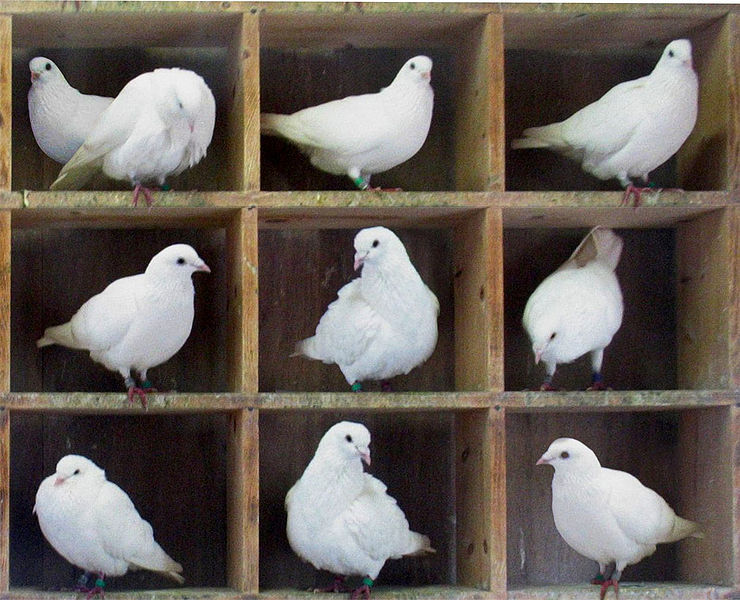
\includegraphics[scale=0.5]{cnt-chapters/toomanypigeons}
\caption{From http://en.wikipedia.org/wiki/File:TooManyPigeons.jpg}
\end{figure}

There are two basic questions to ask when applying the pigeonhole principle:
\begin{enumerate}
\item
What are the pigeons?
\item
What are the holes?
\end{enumerate}
Often the solution to a difficult problem hinges on the correct answer to these two questions; sometimes the pigeons and boxes have to be chosen in creative ways!
\begin{ex}
Let $A$ be a set of $n$ integers. Prove that $A$ contains a subset such that the sum of its elements is divisible by $n$.
\end{ex}
\begin{proof}
Label the elements of $A$ as $a_1,\ldots,a_n$.  
Define the partial sums
\begin{align*}
s_0&=0\\
s_1&=a_1\\
s_2&=a_1+a_2\\
\vdots&\;\;\;\;\;\vdots\\
s_n&=a_1+a_2+ \cdots+a_n.
\end{align*}
Since there are $n+1$ numbers and $n$ possible residues modulo $n$, by the Pigeonhole Principle two of them, say $s_i$ and $s_j$, have the same residue modulo $n$. Suppose without loss of generality that $i<j$. Then 
\[s_j-s_i=a_{i+1}+\cdots +a_j\]
is divisible by $n$, as needed.

Here the pigeons are the partial sums, and the holes are the residues modulo $n$. Note that we considered the partial sums, so that the difference of two of them is a sum of elements of $A$. 
\end{proof}
\begin{thm}[Dirichlet/Kronecker] Let $a$ be a real number and $\ep>0$. Then there exists a positive integer $p$ and an integer $m$ such that $\left|pa-m\right|< \ep$.
\end{thm}
In other words, given any number, we can find a multiple of it that is as close to an integer as we want.
\begin{proof}
Equivalently, we want to find $p$ such that $\{pa\}$ is either in $[0,\ep)$ or $(1-\ep,1)$, because then we could either set $m=\fl{pa}$, ($pa$ rounded down to the nearest integer) or $m=\ce{pa}$ ($pa$ rounded up to the nearest integer). Hence we just focus on the fractional parts of the multiples of $a$. We note that if $\{pa\}$ and $\{qa\}$ are close together, then $|p-q|a$ will be close to an integer. We make this precise below. 

Choose an integer $N$ such that $N\ge\rc{\ep}$. 
The elements $\{pa\}$ for $1\leq p\leq N+1$ fall in one of the $N$ intervals
\[\left[\frac{0}{N},\frac{1}{N}\right),\left[\frac{1}{N},\frac{2}{N} \right),\ldots, \left[\frac{N-1}{N},\frac{N}{N}\right).\]
By the Pigeonhole Principle, two of the $\{p\al\}$ fall in the same interval, say $p\al$ and $q\al$. Then 
$\{|p-q|\al\}\in \left[ 0,\rc{N}\right) \cup \left(\frac{N-1}{N},1\right)
\subeq[0,\ep)\cup(1-\ep,1)
,$
as needed.

In this problem the pigeons are the fractional parts and the holes are the intervals above.
\end{proof}
\begin{rem}
The above proof shows that one of the numbers $a,\ldots, Na$ is at most a distance of $\rc{N}$ away from an integer. Can you show that in fact one of the numbers $a,\ldots, (N-1)a$ is at most at distance of $\rc{N}$ from an integer?
\end{rem} 
%\pagebreak
{\Large Problems 1}
\begin{enumerate}
\item Prove that if one chooses more than $n$ numbers from the set
$\{1,2,3,...,2n\}$, then 
\begin{enumerate}
\item two of them are relatively prime, and 
\item one number is a multiple of another.
\end{enumerate}
\item Prove that for every $n$, there is a nonzero Fibonacci number divisible by $n$. (The Fibonacci numbers are defined by $F_0=0, F_1=1$ and $F_{n+2}=F_{n+1}+F_n$.)
\item A set $S$ of distinct integers each of which is greater than or equal to 1 and less than or equal to $n$ is given. 
\begin{enumerate}
\item If $S$ consists of $\fl{\frac n2}+1$ elements, is it possible that no element of $S$ is the sum of two \textbf{distinct} elements of $S$? 
\item If $S$ consists of $\fl{\frac n2}+2$ elements, prove that the largest element of $S$ is the sum of 2 distinct elements of $S$ and the smallest element is the difference of two distinct elements of $S$. 
\item 
Find the smallest positive integer $m$ (in terms of $n$) such that if $S$ has $m$ elements, then some element of $S$ is the sum of 3 distinct elements of $S$.
\end{enumerate}
\item Prove that any subset of $\{1,\ldots, n\}$ with at least $\fl{\frac{n+k}{2}}+1$ elements contains two elements differing by $k$.
\item (Putnam 2006/B2) Prove that for every set $X=\{x_1,\ldots, x_n\}$ of real numbers, there exists a non-empty subset $S$ of $X$ and an integer $m$ such that 
\[\ab{m+\sum_{s\in S} s}\leq \rc{n+1}.\]
\item (IMO 1972/1) Let $S$ be a set of 10 arbitrary 2-digit numbers. Prove that one can
find two disjoint subsets of $S$ with the same sum of elements.
\item (Romania) Find the greatest positive integer $n$ with the following property:
there exist $n$ nonnegative integers $x_{1},x_{2},\ldots,x_{n}$, at least one
different from zero, such that for any numbers $a_{1},a_{2},\ldots,a_{n}
\in\left\{  -1,0,1\right\}$, at least one different from zero, $n^{3}$ does
not divide $a_{1}x_{1}+a_{2}x_{2}+\ldots+a_{n}x_{n}$.
\item Given 25 positive integers all of whose prime factors are in the set $\{2,3,5\}$, prove that there are 4 numbers whose product is the 4th power of an integer.
\item Let $a_1,\ldots, a_n$ be real numbers. Show that for any $\ep>0$ there exists a positive integer $p$ and integers $m_i$ so that
\[|pa_i-m_i|<\ep\]
for all $i$. 
\item For a positive real number $a$, let $S_a=\{\fl{na}|n\in \N\}$. Do there exist $a,b,c$ such that $S_a,S_b$, and $S_c$ are disjoint? (Hint: Use the previous problem.)
\item Let $S$ be a set of $n$ positive integers, and let $m$ be a positive integer. Prove that there are at least $2^{n-m+1}$ subsets of $S$ with sum of elements divisible by $m$. Include the empty set in your count. 
\item (Romania 1996) Let $n$ be an integer greater than 2 and let $S$ be a $3n^2$ - element subset of the set $\left\{1,2,\ldots,n^3\right\}$. Prove that one can find nine distinct numbers $a_{1},a_{2},\ldots,a_{9}$ in $S$ such that the system
\begin{align*}
a_{1}x+a_{2}y+a_{3}z&=0\\
a_{4}x+a_{5}y+a_{6}z&=0\\
a_{7}x+a_{8}y+a_{9}z&=0
\end{align*}
has a solution $(x_{0},y_{0},z_{0})$ in nonzero integers.

\item (\cite[\S 7.4]{Nat}) Let $A$ be a subset of the nonnegative integers $\N_0$ containing 0. Let $A(n)$ denote the number of nonzero elements of $A$ that are at most $n$, i.e. $A(n)=|A\cap [1,n]|$. Define the \textbf{Shnirel'man density} of $A$ to be{\footnote{The {\it infimum} of a set is like the minimum of the set. It is defined as the greatest lower bound for the set, so unlike the minimum it is always defined. For example, the infimum of the set $S=\{x|x>0\}$ is 0; however the minimum does not exist, because 0 is not in the set itself.}}
\[
\sigma(A)=\inf_{n\geq 1} \frac{A(n)}{n}.
\]
For two sets $A,B$, define the sumset to be all possible sums of an element in $A$ and an element in $B$:
\[
A+B=\{a+b\mid a\in A,b\in B\}.
\]
(The difference $A-B$ is defined similarly.) Define
\[
nA=\underbrace{A+\cdots +A}_n,
\]
i.e. $nA$ consists of numbers that are the sum of $n$ elements of $A$. We say that $A$ is a \textbf{basis} of order $n$ if $nA=\N_0$. 
Prove the following:
\begin{thm}[Shnirel'man] 
If $\sigma(A)>0$ then $A$ is a basis of finite order.
\end{thm}
Hints:
\begin{enumerate}
\item
Show that if $\sigma(A)+\sigma(B)\geq 1$, then $A+B=\N_0$. Conclude that if $\sigma(A)\geq \rc 2$, then $A$ is a basis of order 2. 
\item 
Prove that $\sigma(A+B)\geq \sigma(A)+\sigma(B)-\sigma(A)\sigma(B)$. (Note: it is true, although harder to prove, that $\sigma(A+B)\geq \min(1,\sigma(A)+\sigma(B))$.)
\item Using (b), show that there exists $m$ so that $\sigma(mA)\geq \rc 2$, and using (a), conclude the theorem.
\end{enumerate}
Shnirel'man density can be used to give a proof of a weaker form of Goldbach's conjecture: There exists $n$ so that every integer greater than 1 is the sum of at most $n$ primes. Letting $A$ be the set of sums of two primes along with 0 and 1, the first step is showing that $A$ has positive Shnirel'man density. See~\cite[\S 7.5]{Nat}.
\end{enumerate}
\section{Counting in Two Ways and Probability}
\begin{ex}
Prove that the set $\{1,2,\ldots, 2010\}$ can be colored with two colors such that each of its (nonconstant) arithmetic sequences with 18 terms is not monochromatic.
\end{ex}
\begin{proof}
It is difficult to explicitly describe such a coloring! Indeed, any coloring we describe, short of writing out the colors of every single number, will probably have some pattern to it, and here we want a ``disorderly" coloring, one in which long arithmetic sequences do not have the same color. So instead, we take an indirect approach.

For a coloring $C$ of $\{1,2,\ldots, 2010\}$ with 2 colors, let $f(C)$ be the number of distinct nonconstant monochromatic 18-term arithmetic sequences resulting from the coloring. We want to prove that $f(C)=0$ for some coloring $C$. Consider the sum of $f(C)$ over all colorings, $\sum_C f(C)$. We will express this sum in another way.

Note that this sum counts the number of pairs $(C, \{a_n\}_{n=1}^{18})$ where $C$ is a coloring of $\{1,\ldots, 2010\}$ and $\{a_n\}_{n=1}^{18}$ is an 18-term arithmetic sequence monochromatic under $C$, by summing over $C$. We can instead count the number of such pairs by summing over all valid sequences. To do this we need to answer two questions.
\begin{enumerate}
\item How many 18-term arithmetic sequences with values in $\{1,2,\ldots, 2010\}$ are there? Suppose the common difference is $d$, where $1\leq d\leq \fl{\frac{2010-1}{17}}=118$. In order for the sequence to have values in $\{1,\ldots, 2010\}$, we must have $a+17d\leq 2010$, giving $1\leq a\leq 2010-17d$, i.e. there are $2010-17d$ possibilities for $a$. Summing over $d$, the total number of valid sequences is
\[\sum_{d=1}^{118} (2008-17d)=\frac{118}{2}(1993+4)=117823.\]
\item For a given arithmetic sequence, in how many colorings is it monochromatic? The answer is the same for all sequences: $2\cdot 2^{2010-18}=2^{2010-17}$, since we can color the sequence in one of 2 colors, and each of the remaining $2010-18$ elements can be colored in one of 2 ways.
\end{enumerate}
Thus
\[\sum_C f(C)=117823\cdot 2^{2010-17}< 2^{17}\cdot 2^{2010-17}=2^{2010}.\]
Since there are $2^{2010}$ colorings, this means that we must have $f(C)<1$ for some $C$. Then $f(C)=0$, and that $C$ is our desired coloring. (In other words, the number of instances where a monochromatic 18-term arithmetic sequence appears in a coloring is less than the number of colorings, so one coloring must have no such sequence.)
\end{proof}

It is instructive to look at the above proof in another way, through a more probabilistic lens. We could ask ourselves, what is the \textbf{expected value} of the number of monochromatic arithmetic sequences, if each number is colored with one of the two colors independently with probability $\rc 2$? If we prove that the expected value is less than 1, then we are done. Given a sequence, there is a $\rc{2^{17}}$ chance that it will be monochromatic in our coloring, so
\[
E(f(C))=\frac{117823}{2^{17}},
\]
which is less than 1, as needed.

The two arguments are essentially the same, though there are times when the probabilistic viewpoint is more natural, and furthermore, it allows more advanced probability theory to be used (see problem 4).

{\Large Problems 2}
\begin{enumerate}
\item For which $n$ does there exist a permutation $\sigma$ of $1,\ldots, n$ such that $\sigma(i)+i\pmod n$ are all distinct?
\item (ISL 1999/C4) Let $A$ be a set of $N$ residues modulo $N^2$. Prove that there exists a set $B$ of $N$ residues modulo $N^2$ such that the set $A+B$ contains at least half of all residues modulo $N^2$. (See Problem 1.12 for an explanation of the notation.)
\item (Erd\H os, 1965; TST 2001/3)
A set $A$ is called sum-free if there do not exist $a,b,c\in A$ (not necessarily distinct) such that $a+b=c$. Prove that every set $A$ of $n$ nonzero integers contains a sum-free subset of size greater than $\frac{n}{3}$.
\item (\cite[\S1]{TV}) For a set $A\subeq \N_0$, let $r_A(n)$ denote the number of ways to write $n$ as a sum of two elements of $A$ (order matters). Prove that there exists a basis $A\subeq \N_0$ of order 2 such that $r_A(n)=\Theta(\ln n)$.\footnote{For two functions $f,g$ defined on $\N$, we say that $f(n)=\Theta(g(n))$ if there exist positive constants $c_1,c_2$ such that $c_1g(n)\leq f(n)\leq c_2g(n)$ for all $n$.} We say such a basis is a {\it thin} basis because it is believed be ``smallest" possible basis of order 2.
Hints: 
\begin{enumerate}
\item Define a set $B\subeq \N_0$ randomly by putting each $n\in \N$ into $B$ independently with probability $\min\pa{C\sqrt{\frac{\ln n}{n}},1}$, where $C$ is to be chosen later. For a statement $S$ depending on $B$, define $I(S)$ to be 0 if $S$ is not true, and 1 if $S$ is true. Let
\[r_B'(n)=\sum_{1\leq i<n/2} I(i\in B)I(n-i\in B).\]
Then we have that
\[r_B(n)=2r_B'(n) + a\]
where $a=0$ or 1. (Why?) Show that the expected value satisfies
\[E(r_B'(n))=\Theta(C^2\ln n).\]
\item Prove the following lemma.
\begin{lem}[Borel-Cantelli]
Let $E_1,E_2,\ldots$ be a sequence of events such that $\sum_{n\geq 1} P(E_n)$ is finite. Then there is probability 1 that only finitely many of the events occur.
\end{lem}
\item Using the following theorem from probability, 
show that for some choice of $C$ there are positive constants $c_1,c_2,k$ such that
\[
P(c_1\ln n \leq r_B'(n)\leq c_2\ln n)\leq \frac{k}{n^2}.
\]
\begin{thm}[Chernoff's inequality]
Suppose that $X$ is a sum of independent random variables each of which takes the value 0 or 1. Then for any $\ep>0$,
\[P(|X-E(X)|\geq \ep E(X))\boldsymbol \leq 2e^{-\min(\ep^2/4,\ep/2)E(X)}.\]
\end{thm}
\item Use (b) to finish the proof.
\end{enumerate}
\end{enumerate}
%\pagebreak
\section{Additive Sets}
The Cauchy-Davenport Theorem tells us the minimal size of a sumset in $\Z/p\Z$.
\index{Cauchy-Davenport Theorem}
\begin{thm}[Cauchy-Davenport]\label{cauchy-davenport}
If $p$ is prime, and $A,B$ are nonempty subsets of $\Z/p\Z$, then
\[
|A+B|\geq \min(|A|+|B|-1,p).
\]
\end{thm}
\begin{proof}
We use induction on $|B|$. The base case is when $|B|=1$; in this case $A+B$ simply consists of the elements of $A$ translated by the single element in $B$, so $|A+B|=|A|$, as needed.

Now suppose the theorem is proved for smaller $|B|$. We try to reduce the size of one of the sets and increase the size of the other one, so that we may apply the induction hypothesis. 
If $A\cap B$ were nonempty, then we find that
\begin{align}
\label{capcup}
A\cap B+A\cup B&\subeq A+B\\
\label{samesum}
|A\cap B|+|A\cup B|&=|A|+|B|
\end{align}
Indeed, if $c\in A\cap B$ and $a\in A$, then $c+a\in B+A$, and if $b\in B$, then $c+b\in A+B$, so~(\ref{capcup}) follows. If $A\cap B$ had strictly smaller size than $B$, then we could apply the induction hypothesis to $A\cap B$ and $A\cup B$ to conclude\vspace{-.1cm}
\[
|A+B|\stackrel{(\ref{capcup})}{\geq}|A\cap B+A\cup B|\geq |A\cap B|+|A\cup B|-1\stackrel{(\ref{samesum})}{=}|A|+|B|-1.
\]
In the general case, we note that if we replace $A$ by $A+e$, then $A+B$ would be shifted by $e$ but still have the same size. So if we found $e$ so that $0<|(A+e)\cap B|<|B|$, then we could apply the above argument to $A+e$ and $B$. We choose $e\in B-A$ so that the intersection $(A+e)\cap B$ is nonempty. Suppose we can't find $e\in B-A$ satisfying $|(A+e)\cap B|<|B|$; then for every $e\in B-A$ we have that $|(A+e)\cap B|=|B|$. Then $B\subeq A+e$ for all $e\in B-A$, i.e. $B+e'\subeq A$ for all $e'\in A-B$, so 
\begin{equation}B+(A-B)\subeq A.\label{bab}
\end{equation}
 Take any $a\in A$ and nonzero $c\in B-B$, such as $b_1-b_2$ where $b_1,b_2$ are unequal elements of $B$. Then from~(\ref{bab}) we get $a\in A, a+c\in A$, and $a+kc\in A$ for all positive integers $k$ by induction. But since we are working mod $p$, the multiples of $c$ range over all residues modulo $p$. Hence $A=\Z/p\Z$. In this case, it is obvious that $|A+B|=p$ and we are done.
\end{proof}
One part of additive number theory is finding inequalities involving the sizes of sumsets and other combinations of sets; another part is asking the {\it inverse} question: What can we say about the structure of the sets when the minimum (or something close to it) is attained? In this way Vosper's Theorem is the inverse theorem to Cauchy-Davenport.
\begin{thm}[Vosper]\label{vosper}
Suppose that $p$ is prime, and $A,B$ are subsets of $\Z/p\Z$ such that $|A|,|B|\geq 2$ and $|A+B|\leq p-2$. Then $|A+B|=|A|+|B|-1$ if and only if $A,B$ are arithmetic sequences with the same difference.
\end{thm}
Note that arithmetic sequences in $\Z/p\Z$ may be ``harder to spot" since they can wrap around, for example, $\{2,4,5,7,8,10\}$ is an arithmetic sequence modulo 11 with first term 4 and common difference 3.

\begin{proof}
The ``if" part is easy (and left to the reader). We prove the ``only if" part. We proceed in several steps.
\begin{st}\label{s1}
Prove the theorem when $A$ (or by symmetry, $B$) is an arithmetic sequence.
\end{st}
Suppose that $A=\{a+kd\mid 0\leq k<n\}$. Then 
\begin{align*}
A&=\{a+kd\mid 0\leq k<n-1\}+\{0,d\}\\
A+B&=\{a+kd\mid 0\leq k<n-1\}+(\{0,d\}+B)
\end{align*}
so applying Cauchy-Davenport to the two sets on the right, we get
\begin{align*}
|A+B|\geq (n-1)+|B+\{0,d\}|-1=|B+\{0,d\}|+(n-2).
\end{align*}
However, we know $|A+B|=n+|B|-1$, so these two equations give $|B|+1\geq |B+\{0,d\}|$. We can partition $B$ into arithmetic sequences with step $d$, so that none of these sequences can be extended while staying in $B$. If there are $m$ such sequences, then we find that $|B+\{0,d\}|=|B|+m$ (Why?). Thus $m=1$, and $B$ is an arithmetic sequence with the same step as $A$.

\begin{st}\label{s2}
If $A+B$ is an arithmetic sequence with step $d$, then $A,B$ are arithmetic sequences with step $d$.
\end{st}
The idea here is to apply Step~\ref{s1} with the {\it complement} of $A+B$, $-B$, and the complement of $A$.

Note that extending the arithmetic sequence $A+B$ in one direction will give us the entire set $\Z/p\Z$. Hence 
\[C:=(\Z/p\Z)\backslash (A+B)=\{c\in \Z/p\Z\mid c\neq a+b\text{ for any }a\in A,b\in B \}\]
also be an arithmetic sequence with the same step. 
From the RHS of the above, we see that $c-b\neq a$ for any $a\in A,b\in B,c\in C$, i.e. $C+(-B)\subeq (\Z/p\Z)\backslash A$. Now Cauchy-Davenport says
\[
p-|A|\geq |C+(-B)|\geq |C|+|B|-1=(p-|A+B|)+|B|-1.
\]
However, equality is attained by the given assumption $|A+B|=|A|+|B|-1$, so by Step~\ref{s1} applied to $C, -B$, and $(\Z/p\Z)\backslash A$, we get that $-B$ and hence $B$ is also an arithmetic sequence with same step as $C$. (Note $|C|\geq 2$ since $|A+B|\leq p-2$.) Similarly, $A$ is an arithmetic sequence with the same step.
\begin{st}\label{s3}
Induct on $|B|$.
\end{st}
If $|B|=2$ then $B$ is automatically an arithmetic sequence so just use Step~\ref{s1}. For the induction step, we use the same ``$e$-transform" technique we used in Cauchy-Davenport. Suppose we can find $e\in B-A$ so that $1<|(A+e)\cap B|<|B|$. Now $A+(B-e)\supeq A\cap (B-e)+A\cup (B-e)$ as in~(\ref{capcup}) so $A+B\supeq (A+e)\cap B+A\cup (B-e)$ (make sure you see this!). Hence
\begin{align*}
|A|+|B|-1&=|A+B|\\
&\geq |(A+e)\cap B+A\cup (B-e)|\\
&\geq|(A+e)\cap B|+|A\cup (B-e)|-1\\
&=|A\cap (B-e)|+|A\cup (B-e)|-1\\
&=|A|+|B-e|-1.
\end{align*}
However equality holds, so 
\begin{equation}\label{abe}
(A+e)\cap B+A\cup (B-e)=A+B
\end{equation}
and applying the induction hypothesis to $(A+e)\cap B$ and $A\cup (B-e)$ gives that $(A+e)\cap B,A\cup (B-e)$, and their sumset $(A+e)\cap B+A\cup (B-e)$ are all arithmetic sequences. From~(\ref{abe}) this means $A+B$ is an arithmetic sequence. Using Step~\ref{s2}, we conclude both $A,B$ are arithmetic progressions with the same step.

What happens if we can't find such an $e$? Let $E_1$ be the set of $e$ so that $|(A+e)\cap B|=|B|$, and let $E_2$ be the set of $e$ so that $|(A+e)\cap B|=1$. Since these cover all the bad cases, $|E_1|+|E_2|=|B-A|$. 
Now $e\in E_1$ iff $B\subeq A+e$, or equivalently $B-e\subeq A$. Thus $B-E_1\subeq A$. Using Cauchy-Davenport gives $|B|+|E_1|-1\leq |A|$, that is, \[|E_1|\leq |A|-|B|+1.\]
Then
\[|E_2|=|A-B|-|E_1|\geq (|A|+|B|-1)-(|A|-|B|+1)=2|B|-2.\]
Now $(A+e)\cap B$ is a single element in $B$ for any $e\in E_2$; $|B|>2$ implies $2|B|-2>|B|$, so by the Pigeonhole Principle, there exist $e\neq  e'$ and $b$ such that $(A+e)\cap B=(A+e')\cap B=\{b\}$. Then from~(\ref{abe}), 
\[b+(A\cup (B-e))=A+B=b+(A\cup (B-e'))\]
so
\[
A\cup (B-e)=A\cup (B-e').
\]
Hence $(B-e)\backslash A=(B-e')\backslash A$. 
But $B-e$ has only one element in common with $A$, as $B$ has only the element $b$ in common with $A+e$, and ditto with $B-e'$. Thus $B-e$ and $B-e'$ become equal after removing one element from each; we conclude $B-e$ and $B-e'=B-e+(e'-e)$ can only differ in one element, that is, $B+\{-e,-e'\}$ has $|B|+1$ elements. By Step~\ref{s1}, we get that $B$ is an arithmetic sequence with step $e'-e$. Then by Step~\ref{s1}, $A$ is also an arithmetic sequence with step $e'-e$, finishing the proof.
\end{proof}
\begin{rem}
Note the $|A+B|\leq p-2$ condition is necessary. A counterexample when $|A+B|=p-1$ is when $p=7$, $A=\{0,1,3\}$ and $B=\{0,1,2,4\}$.
\end{rem}
{\Large Problems 3}
\begin{enumerate}
\item Let $A_1,\ldots, A_n$ be nonempty subsets of $\R$. Prove that
\[
|A_1+\cdots +A_n|\geq |A_1|+\cdots +|A_n|-n+1.
\]
When is equality attained? (Do the $n=2$ case first.)
Why does this proof not work for $\Z/p\Z$?
\item
(USAMO 2009/2) Let $n$ be a positive integer. Determine the size of the largest subset of $\{-n,-n+1,\ldots, n-1,n\}$ which does not contain three elements $a,b,c$ (not necessarily distinct) satisfying $a+b+c=0$.
\item Prove the following:
\begin{thm}[Erd\H os-Ginzburg-Ziv]\label{erdos-ginzburg-ziv}
From any $2n-1$ integers we can choose $n$ integers such that their arithmetic mean is also an integer.
\end{thm}
Hint: Prove the theorem for $n$ prime, then show that if the theorem holds for $n=a$ and $n=b$, then it holds for $n=ab$. 
\item Let $p$ be a prime and $d$ a positive integer such that $p>2d+1$. Prove that every residue modulo $p$ is the sum of $\fl{\frac d2}+1$ $d$th powers modulo $p$. (For more on this problem see~\cite{Lee}.)
\end{enumerate}
\section{Coloring Numbers}
Problems involving coloring numbers are quite common (and fun!). Probably the most important tip is just ``play around with the numbers" and see what you can come up with...

\begin{ex}
The set $\{1,2,\ldots, 3n\}$ is partitioned into three sets $A,B,C$ with each set containing $n$ numbers. Then it is always possible to choose one number in each of the three sets such that one of the numbers is the sum of the other two.
\end{ex}
\begin{proof}
Suppose that $A,B,C$ do not satisfy the last condition.

A good place to start is to make some ``without loss of generality" assumptions. Suppose $1\in A$. 1 is going to be an important player because the color of 1 together with the color of $k$ influences the color of $k\pm 1$. Now suppose that the smallest element not in $A$ is in $B$; call this number $b$. Now $C$ has the largest minimal element of all three sets; call this number $c$.

Now, since we are proceeding by way of contradiction, $1\in A, c\in C$ imply that $c-1\nin B$. But $c-1\nin C$ either, by our minimality assumption. Hence $c-1\in A$. See the table on the left.

\begin{figure}[h!]\centering
\begin{tabular}{|c|c|c|}
\hline 
$A$ & $B$ & $C$\tabularnewline
\hline 
1 &  & \tabularnewline
\hline 
$\vdots$ &  & \tabularnewline
\hline 
$b-1$ &  & \tabularnewline
\hline 
 & $b$ & \tabularnewline
\hline 
$\vdots$ & $\vdots$ & \tabularnewline
\hline 
$c-1$ &  & \tabularnewline
\hline 
 &  & $c$\tabularnewline
\hline
\end{tabular}
\qquad
\begin{tabular}{|c|c|c|}
\hline 
$A$ & $B$ & $C$\tabularnewline
\hline 
1 &  & \tabularnewline
\hline 
$\vdots$ &  & \tabularnewline
\hline 
$b-1$ &  & \tabularnewline
\hline 
 & $b$ & \tabularnewline
\hline 
$\vdots$ & $\vdots$ & $\vdots$\tabularnewline
\hline 
 & \multicolumn{2}{c|}{$c'-1-b$ (?)}\tabularnewline
\hline 
 & \multicolumn{2}{c|}{$c'-b$ (?)}\tabularnewline
\hline 
$\vdots$ & $\vdots$ & $\vdots$\tabularnewline
\hline 
 &  & $c'-1$\tabularnewline
\hline 
 &  & $c'$\tabularnewline
\hline
\end{tabular}
\end{figure}

What about for an arbitrary $c'\in C$? $1\in A, c'\in C$ imply that $c'-1\nin B$, so $c'-1\in A$ or $c'-1\in C$. Let's consider what happens in the second case. See the table on the right.

Suppose that $c'$ is {\it minimal} so that $c'\in C$ and $c'-1\in C$. We've already considered the pair $(1\in A, c'\in C)$, so now let's consider the pair $(b\in B, c'\in C)$. This gives that $c'-b\nin A$, i.e. $c'-b\in B$ or $C$. Similarly, $b\in B, c'-1\in C$ give that $c'-1-b\in B$ or $C$. We analyze each case.
If $c'-b\in B$ then $b-1\in A, c'-b\in B, c'-1\in C$ are in different sets, a contradiction. If $c'-b\in C$, then we've already shown $c'-1-b\nin B$. However, the remaining case $c'-b-1,c'-b\in C$ cannot occur by our minimality assumption on $c'$. Hence there cannot exist $c'$ so that $c'$ and $c'-1$ are both in $C$.

We've proven the following key claim.\\

\noindent {\it Claim:} If $c'\in C$ then $c'-1\in A$.\\

Now we use the last piece of information, that $|A|=|B|=|C|$. By the claim, each $c'\in C$ is matched up with a distinct element $c'-1\in A$. However, no element of $C$ is matched up with $1\in A$, since $2\nin C$. Hence $|A|>|C|$, a contradiction. Thus our assumption was wrong, and the problem statement follows.
\end{proof}

Now we'll prove a two famous theorems in combinatorial number theory, following the approach in~\cite[\S6.3]{TV}. The proofs will take quite a bit of work! For convenience, when we write $[a,b]$, we will mean $\{x\in \Z|a\leq x\leq b\}$.

\subsection{Schur's Theorem and Ramsey Theory}
\begin{thm}[Schur]
Given $c,k\geq 1$, there exists $N=S(c,k)$ such that if the integers in $[1,N]$ are colored with $c$ colors, then there exist (not necessarily distinct) $x_1,\ldots, x_k\in [1,N]$ such that $x_1,\ldots, x_k, x_1+\cdots +x_k$ all have the same color.
\end{thm}
To prove this, we recast the theorem in graph theoretic terms. Consider the graph with vertices labeled by $1, \ldots, N+1$, and with an edge between $i,j$ assigned the color of $|i-j|$. Then we are looking for a complete subgraph with $k+1$ vertices, all of whose edges have the same color. Indeed, if we have such a subgraph, whose vertices are labeled with $v_1<\cdots< v_{k+1}$, then we can set $x_i=v_{i+1}-v_i$. Then the $x_i$ and $x_1+\cdots +x_k=v_{k+1}-v_1$ all have the same color.

So Schur's Theorem will follow from a more general theorem about graphs:
\index{Ramsey's theorem}
\begin{thm}[Ramsey]\label{ramsey}
Given any positive integers $n_1,\ldots, n_c$, there exists $N$ such that if a complete graph with $N$ vertices is colored with $c$ colors $1,\ldots, c$, then there is a complete subgraph with $n_i$ vertices, all of whose edges are colored with color $i$, for some $i$.
\end{thm}
For short, we say that a subgraph all of whose edges are colored with $i$, is of color $i$. 
We define $R(n_1,\ldots, n_c;c)$ to be the {\it least} value of $N$ that works above.

For Schur's Theorem, we can take $S(c,k)=R(k+1,\ldots, k+1;c)-1$; then the graph we considered above will have $R(k+1,\ldots, k+1;c)$ vertices, and so be forced to have a subgraph with $k+1$ vertices, with all edges the same color.

Now we prove Ramsey's Theorem.
\begin{proof}
The case $c=1$ is trivial; the case $c=2$ will be the base case of our induction. 

For $c=2$, we induct on $m+n$.
When either $m$ or $n$ is 1 (say $n=1$), then the claim is trivial as any subgraph with 1 vertex has no edges, and we may take $R(m,n;2)=1$. Now suppose the claim proved for $m'+n'<m+n$. We show that
\begin{equation}\label{ram}
R(m,n;2)\leq R(m-1,n;2)+R(m,n-1;2).
\end{equation}
Take any graph with $R(m-1,n;2)+R(m,n-1;2)$ vertices, whose edges are colored in 2 colors, say red and blue. Take any vertex $V$. There are $R(m-1,n;2)+R(m,n-1;2)-1$ edges leading out of it. Thus either at least $R(m-1,n;2)$ of those edges are red, or at least $R(m,n-1;2)$ of those edges are blue. We consider the first case; the second case follows by the same argument. Let $V_1,\ldots, V_i$ be the vertices that $V$ is connected to by a red edge, and consider the subgraph induced by $V_1,\ldots, V_i$.  Since $i\geq R(m-1,n;2)$, either it has a complete red subgraph with $m-1$ vertices, or a complete blue subgraph of $n$ vertices. In the second case we are done; in the first case, adjoining $V$ gives a complete red subgraph of $m$ vertices, as needed.

Now we induct on $c$. Supposing $c>2$ and that the theorem is true for $c-1$, we show
\[
R(n_1,\ldots, n_c;c)\leq R(R(n_1,\ldots, n_{c-1};c-1),n_c;2).
\]
Take a graph with $R(R(n_1,\ldots, n_{c-1};c-1),n_c;2)$ vertices and colored in $c$ colors, say blah, blah, \ldots, and purple. Temporarily recolor the first $c-1$ colors with gray. Then there exists a gray subgraph with $R(n_1,\ldots, n_{c-1};c-1)$ vertices, or a purple subgraph with $n_c$ vertices. We are done in the second case; in the first case, we scrape off the gray paint, revealing that all edges in our subgraph are one of the first $c-1$ colors. Then by definition of $R$, there is a subgraph of color $i$, with $n_i$ vertices, for some $1\leq i\leq c-1$, and we are again done.
\end{proof}
Note that~(\ref{ram}) and Pascal's Identity give that $R(m,n;2)\leq \binom{m+n-2}{m-1}$.

\subsection{Van der Waerden's Theorem}
\index{Van der Waerden's Theorem}
\begin{thm}[Van der Waerden] \label{vdw}
For every $c\geq 1$ and every $n\geq 1$, there exists $N$ so that if the integers in $[0,N]$ are colored with $c$ colors, then there is a monochromatic arithmetic sequence of length $n$.

As a corollary, if the nonnegative integers are colored with a finite number of colors, then there exists arbitrarily long monochromatic arithmetic sequences.
\end{thm}
One way to prove this is to recast this problem into a higher-dimensional problem!{\footnote{It is possible to proceed more directly; see \url{http://www.math.uga.edu/~lyall/REU/VW.pdf}}} Consider the integers in $[0,n^d)$ for some large $d$. By writing an integer in this interval in base $n$, we can view it as a point in a $d$-dimensional hypercube with side length $n-1$. Specifically, identify $a_{d-1}n^{d-1}+\cdots +a_1n+a_0$ with the point $(a_0,a_1,\ldots, a_{d-1})\in [0,n-1]^d$. If $n$ points in this hypercube are on the same line and spaced equally apart (in which case we say they are in arithmetic sequence), then they correspond to a $n$-term arithmetic sequence in $[0,n^d)$. Hence it suffices to prove the following stronger theorem.

\index{Hales-Jewett Theorem}
\begin{thm}[Hales-Jewett] Given $c,n\geq 1$, there exists an integer $d=d(n,c)$ such that if $[0,n-1]^d$ is colored with $c$ colors, then there is a nonconstant arithmetic progression $a+[0,n-1]v=\{a,a+v,\ldots, a+(n-1)v\}$ of length $n$, for some $a\in [0,n-1]^d$ and $v\in [0,1]^d$.
\end{thm}
For example, if $a=(0,0,1),v=(1,1,0)$, and $n=3$, then $a+[0,n-1]v$ is the sequence $(0,0,1), (1,1,1), (2,2,1)$. This theorem basically says we can force the existence of arithmetic progressions by making the dimension of the hypercube large enough. After we find $d$ as in the theorem, taking $N=n^d-1$ will do for Van der Waerden's Theorem.

To prove Hales-Jewett, we will prove a yet more general statement, by double induction. Define a \text{stick} of length $n$ to be a $n$-term nonconstant monochromatic arithmetic sequence $a+[0,n-1]v$. Define a \textbf{rainbow $m$-fan} of length $n$ to be a $m+1$-tuple $(a,v_1,\ldots, v_m)$ such that the $(n-1)$-term sequence $a+[1,n-1]v_i$ is monochromatic of a different color for each $i$. We call $a$ the {\it base} of the fan, the $a+[1,n-1]v_i$ the $m$ {\it sticks} of the fan (of length $n-1$), and the colors of $a+[1,n-1]v_i$ the {\it colors} of the fan.

\begin{clm}
Let $c,n\geq 1$ and $1\leq m\leq c$. Then there exists $d=d(n,c,m)$ such that if $[0,n-1]^d$ is colored with $c$ colors, then there exists a stick or a rainbow $m$-fan of length $n$.
\end{clm}
Taking $m=c$ recovers the Hales-Jewett Theorem: If there exists a stick of length $n$ we are done; else there is a rainbow $c$-fan. But any rainbow $c$-fan must contain all the colors, and in particular the color of the base. So one of the sticks (of length $n-1$) is the same color as the base, giving a stick of length $n$ (i.e. a monochromatic arithmetic sequence of length $n$), as needed. Now we prove the claim.

\begin{proof}
The outer induction is on $n$, and the inner induction is on $m$. The base case $n=1$ is trivial (the hypercube is just the point $\mathbf 0$). Assume the theorem proved for $n-1$.

Now we enter the inner induction, on $m$.
\begin{enumerate}
\item
The base case $m=1$: The Hales-Jewett Theorem for $n-1$ is a statement about the hypercube $[0,n-2]^d$. By shifting, it says that there is a $(n-1)$-term arithmetic sequence $a+[0,n-2]v$ contained in $[1,n-1]^d$, with $v\in [0,1]^d$. Then taking $a'=a-v$, we see that $(a,v)$ is a rainbow 1-fan (a somewhat degenerate fan with only one stick).
\item
The induction step: Assume the claim true for $m-1$. Now set
\[d_1=d(n,c,m-1),\quad d_2=d(n-1,c^mn^{d_2m})=d(n-1,c^mn^{d_2m},c^mn^{d_2m}), \quad d=d_1+d_2.\]
(The choice for $d_2$ will become clear later.) 
Each element of $[0,n-1]^d$ can be written as $(x_1,x_2)$, where $x_1\in [0,n-1]^{d_1}$ and $x_2\in [0,n-1]^{d_2}$. Fixing $x_2$, we get a cross section of $[0,n-1]^d$ which is just a $d_1$-dimensional hypercube.
We identify $[0,n-1]^{d_1}$ with the cross section $\{(x_1,x_2)\mid x_1\in [0,n-1]^{d_1}\}$.
By definition of $d_1$, we can find a stick $a_1+[0,n-1]v$ in $[0,n-1]^{d_1}$, or a rainbow $(m-1)$-fan $(a_1,v_1,\ldots, v_{m-1})$ whose sticks are colored differently from the base (if the base is the same color as a stick we are in the first case). In the first case, we get a stick for $[0,n-1]^d$ where the $[0,n-1]^{d_2}$-coordinates are constant, namely $(a_1,x_2)+[0,n-1](v,0)$, and we are done. So suppose the second case holds for every $x_2$; we need to make our $(m-1)$-fan into a $m$-fan. We do this by extending it via the $[0,n-1]^{d_2}$-coordinate.

\begin{figure}[h!]\centering
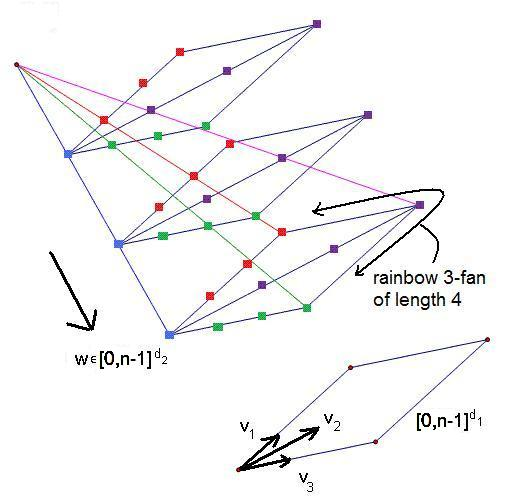
\includegraphics{cnt-chapters/hales-jewett}
\end{figure}

Now for each $x_2$ we have the following pieces of data.
\begin{enumerate}
\item
The base $a_1$ and vectors $v_1,\ldots, v_{m-1}$ in $[0,n-1]^{d_1}$ as defined above: There are at most $(n^{d_1})^m$ possibilities for these.
\item
The colors $C, C_i$ of the base $a_1$ and the sticks $a_1+[1,n-1]v_i,1\leq i\leq m-1$: There are at most $c^m$ choices for these colors.
\end{enumerate}
Hence there are at most $c^mn^{d_1m}$ possibilities for the combined data. Color the points of $[0,n-1]^{d_2}$ with $c^mn^{d_1m}$ colors based on the associated data. 

By the choice of $d_2$, there is a stick of length $n-1$, say (by shifting as in part 1) $a_2+[1,n-1]w$.  
Let the common data for the $n-1$ points in the bar $a_2+[1,n-1]w$ be $a_1,v_1,\ldots, v_{m-1}, C, C_1,\ldots, C_{m-1}$. Now let $a=(a_1,a_2)$; extend the vectors $v_i$ in the $v$-direction by setting $w_i=(v_i,w)$, and include the additional vector $w_m=(0,w)$. See the picture.

We claim that $(a,w_1,\ldots, w_m)$ is a rainbow $m$-fan of length $n$ (in the original coloring). Indeed, the stick $a+[1,n-1]w_i=(a_1,a_2)+[1,n-1](v_i,w)$ has the color $C_i$, the color of corresponding stick in the common cross section. Furthermore, the color of $a+[1,n-1]w_m=a+[1,n-1](0,w)$ is just $C$, the color of the base of the common fan in the cross sections, which is different from the colors $C_1,\ldots, C_{m-1}$. Hence we get a rainbow $m$-fan of length $n$, as needed, completing the induction step.
\end{enumerate}
\end{proof}
It is an interesting exercise to find an explicit value of $N$ that works in Van der Waerden's Theorem by following the above argument.\\

{\Large Problems 4}
\begin{enumerate}
\item If the nonnegative integers are colored with a finite number of colors, does there necessarily exist an infinite monochromatic arithmetic sequence?
\item (HMMT 2009) Find the smallest number of colors needed to color the nonnegative integers so that $a,b$ have different colors whenever $|a-b|$ is a power of 2.
\item (UM 2006) Each positive integer is assigned one of three colors. Show that there exist distinct positive integers $x,y$ such that $x$ and $y$ have the same color and $|x-y|$ is a perfect square.
\item (IMO 1978/6) An international society has members from six different countries. The list of members contains 1978 names, numbered $1,2,\ldots, 1978$. Prove that there is at least one member whose number is the sum of the numbers of two members, not necessarily distinct, of his or her own country.
\item (ISL 1999/C6) Suppose that every integer has been given one of the colors red, blue, green, yellow. Let $x$ and $y$ be odd integers such that $x\neq y$. Show that there are two integers of the same color whose difference is one of the following values: $x,y,x+y,x-y$.
\item (ISL 1995/N7) Does there exist an integer $n>1$ that satisfies the following condition?

The set of positive integers can be partitioned into $n$ nonempty subsets such that an arbitrary sum of $n-1$ integers, one taken from each of any $n-1$ of the subsets, lies in the remaining subset.
\item (ISL 1999/A4) Prove that the set of positive integers cannot be partitioned into three nonempty subsets such that for any two integers $x,y$ taken from two different subsets, the number $x^2-xy+y^2$ belongs to the third subset.
\item (Gallai's Theorem) Given $k,d,c\geq 1$ and $v_1,\ldots, v_k\in \Z^d$, prove that there exists $N$ such that when the points of $[1,N]^d$ are colored with $c$ colors, there exist $x$ and $r\in \Z-\{0\}$ such that $x+rv_1,\ldots, x+rv_k$ all have the same color. 
\end{enumerate}
%%\part{Computational Number Theory}
%%\chapter{Diophantine sets}
\section{Diophantine sets}
\begin{df}
Let $R$ be an integral domain. A \textbf{Diophantine equation} over $R$ is an equation of the form
\[
P(x_1,\ldots, x_n)=0
\]
where $P$ is a polynomial with coefficients in $R$. If $R$ is omitted, we assume that $R=\Z$.
\end{df}
\begin{df}
Let $A\subeq R^m$. 
$A$ is \textbf{Diophantine} if there exists a Diophantine equation in parameters $a_1,\ldots, a_m$ and variables $x_1,\ldots, x_n$, such that $A$ is the set of $(a_1,\ldots, a_m)$ for which the equation is solvable. In other words,
\[
A=\set{(a_1,\ldots, a_m)\in R^n}{P(a_1,\ldots, a_m,x_1,\ldots, x_n)=0\text{ has a solution}}.
\]
We say a property is Diophantine if the set of elements with that property is Diophantine. We say a function $f:R\to R$ is Diophantine if its graph $\set{(x,f(x)}{x\in R}$ is Diophantine.
\end{df}
The following says that all systems of Diophantine equations can be reduced to a single Diophantine equation. Hence we can just consider the special case of a single Diophantine equation.
\begin{pr}
Let $K=\Frac(R)$, suppose $K$ is not algebraically closed, and let $f_1,\ldots, f_m$. 
There exists $g(x_1,\ldots, x_n)$ such that 
\[
g(x_1,\ldots, x_n)=0
\iff\begin{cases}
f_1(x_1,\ldots, x_n)=0\\
\qquad\qquad \vdots \\
f_m(x_1,\ldots, x_n)=0
\end{cases}
\]
\end{pr}
\begin{proof}
By induction it suffices to prove this for the $n=2$ case. 
Take a polynomial $h=\sum_{k=0}^r a_k x^k\in R[x_1,\ldots, x_n]$ with no roots in $K$, and let
\[
g:=h\pf{f_1}{f_2}f_2^r=\sum_{k=0}^r a_kf_1^kf_2^{r-k}.
\]
If $(x_1,\ldots, x_n)$ is a solution of $f_1=f_2=0$ then it is a solution of $h=0$. Suppose by way of contradiction $(x_1,\ldots, x_n)$ is a solution of $h=0$ but $f_1(x_1,\ldots, x_n)$ and $f_2(x_1,\ldots, x_n)$ are not both 0. Then neither is 0 and $\frac{f_1(x_1,\ldots, x_n)}{f_2(x_1,\ldots, x_n)}$ is a root of $h=0$ in $K$, contradiction. 
\end{proof}
\begin{ex}
For $R=\Z$ take $g=X^2+1$. In this case $h=f_1^2+f_2^2$, and it is clear that $h=0$ has a solution in $\Z$ iff $f_1=f_2=0$ has a solution.
\end{ex}
\begin{pr}
Hilbert's tenth problem is true for $\Z$ if and only if it is true of $\N$.
\end{pr}
\begin{proof}
Lagrange's theorem! (sum of 4 squares)
\end{proof}
BIG THM.
Related notion
\begin{df}
A set $A\subeq K^m$ is \text{field-Diophantine} over $R$ if there there exists a polynomial $P(a_1,\ldots, a_m,b,x_1,\ldots, x_n)$ with coefficients in $R$ such that 
\[
A=\set{(a_1,\ldots, a_m)}{P=0\text{ has a solution with }b\ne 0}.
\]
\end{df}
\begin{pr}
The union of two (field-)Diophantine equations is also Diophantine. If $K$ is not algebraically closed the intersection of two (field-)Diophantine equations is also Diophantine.
\end{pr}
\begin{proof}
For the union, take products. For the intersection, similar to proof above.
\end{proof}
\begin{thm}[DPRM theorem]
The Diophantine sets over $\Z$ coincide with the recursively enumerable sets.
\end{thm}
\begin{thm}[Hilbert's tenth problem]
There is no algorithm to decide whether a Diophantine equation over $\Z$ has a solution.
\end{thm}
\begin{thm}
The set of prime numbers is Diophantine.
\end{thm}
\begin{thm}[Existence of prime-producing polynomials]
There exists a nonconstant multivariate polynomial
$P(x_1,\ldots, x_n)\in R[x_1,\ldots, x_n]$ whose positive range is exactly the prime numbers, i.e.
\[
\im(P)\cap \N=\{\text{prime }p\}.
\]
\end{thm}
\begin{proof}
Since the set of prime numbers is Diophantine, there exists $Q$ such that $Q(a,\vec{x})=0$ iff $a$ is prime. Now take 
\[P=a(1-Q^2).\]
\end{proof}
%%\part{Abelian Varieties}

\appendix

\chapter{Multiplication modulo $n$}
\label{multiplicative}

\section{Introduction}
In Chapter~\ref{mod} you learned how modular arithmetic works: you fix a number $n$, and then compute by taking all integers modulo $n$, that is, you throw away all information except the remainder when dividing by $n$. This system obeys all the ``rules" we expect it to, and is especially well-behaved when $n$ is a prime.

%While addition modulo $n$ is relatively transparent, multiplication is a more complicated. 
There is a lot of similarity between addition and multiplication modulo $n$, but it seems multiplication is less ``transparent." Compare the following.
\begin{enumerate}
\item
We saw how we could use modular arithmetic to solve problems such as: what is the last digit of $7\cdot 2011$? What is the last digit of $7^{2011}$? 

You probably see immediately the first answer is 7. To solve the second problem we looked for a repeating pattern in the powers of 7 modulo 10: 1, 7, 9, 3, $\ldots$ We have $7^4\equiv 1\pmod{10}$, so the ``cycle" repeats after every 4 times, and $7^{2011}\equiv 7^3\equiv 3\pmod{10}$.

Making an analogy, note that if look at the sequence $7, 2\cdot 7, 3\cdot 7,\ldots$ we get back to 0 after 10 steps, while in the sequence $7, 7^2, 7^3$ we get back to 1 after 4 steps. It's easy to understand how the cycle repeats when we add repeatedly (i.e., multiply), but what about when we multiply repeatedly (i.e., take powers)?

In general, given $a\pmod n$, how many times do we have to multiply $a$ by itself to get back to 1 (what is the ``order" of $a$ modulo $n$)? How does this depend on $a$ and $n$? Is there some general rule that determines the order?
\item We have the notion of inverses. For instance, what is the additive inverse of 7 modulo 19, i.e., what do we add to 7 to get 0 modulo 19? It is simply $-7\equiv 12\pmod{19}$, because
\[
7+12\equiv 0\pmod{19}.
\]
What is the multiplicative inverse of 7 modulo 19, i.e., what do we multiply 7 by to get 1 modulo 19? You might have to think a bit more on this one---it is $11\pmod{19}$, because
\[
7\cdot 11= 77\equiv 1\pmod{19}.
\]
\end{enumerate}

In this chapter you will learn to completely determine the multiplicative structure of the integers modulo $n$. In Section~\ref{sec:order}, we will make formalize the notion of the \textbf{order} of an element: how many times we have to multiply a number to get back to 1 modulo $n$. We will develop a toolbox of basic theorems: Euler's Theorem and Fermat's Little Theorem in Section~\ref{sec:euler-thm} and Wilson's Theorem in Section~\ref{sec:wilson}. Euler's Theorem will give us $m$ such that  $a^m\equiv 1\pmod{n}$.

We will use these theorems to solve a variety of problems in Section~\ref{sec:mod-ex}. For instance (keepin in the theme of repeating patterns) we will explain why the period of the repeating decimals $\rc{17}$ and $\rc{19}$ are 16 and 18:
\begin{align*}
\rc{17}&=.\underbrace{\overline{0588235294117647}}_{16}\\
\rc{19}&=.\ub{\overline{052631578947368421}}{18}.
\end{align*}
%%

At this point we find that a lot of the stuff we've been doing works in a much more {\it abstract} setting, that of \textbf{groups}. In Section~\ref{groups} we recast all the theorems in the language of group theory, and in this way give a way think about the similarities behind addition and multiplication modulo $n$. With the language of group theory, we give a complete characterization of the multiplicative structure of $\Z/n\Z$ in Sections~\ref{primitive-roots} and~\ref{sec:mult-structure}.

Finally we give two applications, to primality testing (Section~\ref{sec:prime-test}) and basic cryptography (Section~\ref{sec:basic-crypto}).

\section{Order of an element}\llabel{sec:order}
%Let $a$ and $n > 1$ be relatively prime positive
%integers.  Then we know that there exist infinitely many positive
%integers $k$ with $a^k\equiv1\mod{n}$; for example, $k =
%m\varphi(n)$ for an arbitrary positive integer $m$.  Here we develop
%further the theory of such congruences; indeed, 
% This fact provides a
%useful technique for solving advanced problems in number theory.

%Given $a, n$ ($n > 1$) positive integers with $\gcd{(a,n)} = 1$, we let $\text{ord}_n(a)$ denote the smallest positive integer $d$ such that $a^d\equiv1\mod{n}$.  This quantity is called the order of $a$ modulo $n$.  We claim that $\text{ord}_n(a)$ obeys several useful properties.
%\begin{pr}
%Given $a, n$ positive integers with $n > 1$, and let $m$ be a positive integer.  Then $a^m \equiv 1\mod{n}$ if and only if $\textup{ord}_n(a)\mid m$.
%\begin{proof}
%Let $d = \text{ord}_n(a)$.  Then if $m = kd$, then we have $a^m =
%(a^d)^k \equiv 1^k \equiv1\mod{n}$.  Now if $a^m \equiv 1$ and $d
%\nmid m$, set $m = dq + r$, where $0 < r < d$.  Then we have $a^m =
%(a^d)^qa^r \equiv a^r\mod{n}$.  Hence $a^r\equiv a^m\equiv1\mod{n}$.
%But this contradicts the minimality of $d$; hence if
%$a^m\equiv1\mod{n}$ we must have $d \mid m$.
%\end{proof}

%In this chapter we will be concerned with the multiplicative structure of numbers modulo $n$. We will be especially interested in the values taken by powers of an element modulo $n$. We find that they 
We've seen that the values taken by a powers of an element modulo $n$ form a repeating pattern, and under certain relative primality conditions, start each cycle at 1. For example,
\begin{align*}
3^0&\equiv 1\pmod{5}\\
3^1&\equiv 3\pmod{5}\\
3^2&\equiv %9
4\pmod{5}\\
3^3&\equiv %7
2\pmod{5}\\
3^4&\equiv 1\pmod{5}\\
3^5&\equiv 3\pmod{5}, 
\end{align*}
so the powers of 3 cycle 1, 3, 4, 2, $\ldots$ modulo 5.
In particular, we get back to 1 in 4 steps: $3^4\equiv 1\pmod{5}$. Hence we call 4 the {\it order} of 3:
\index{order}
\begin{df}
Let $n>1$ and let $a$ be an integer relatively prime to $a$. 
The \textbf{order} of $a$ modulo $n$ is the smallest positive integer $m$ such that $a^m\equiv 1\pmod{n}$. In symbols,
\[
\ord_n(a)=\min\set{m\in \N}{a^m\equiv 1\pmod{n}}.
\]
\end{df}
For example,
\[
\ord_5(3)=4.
\]
Note that we place the modulus as an 

Note that the order is well-defined for all $a$ relatively prime to $n$: Indeed, there are only a finite number of residues modulo $n$, so two powers of $a$ must be equal modulo $n$. So suppose $0<m_1<m_2$ and
\[
a^{m_1}\equiv a^{m_2}\pmod{n}.
\]
Since $a$ is relatively prime to $n$, we can take inverses to find
$a^{m_2-m_1}\equiv 1\pmod{n}$.

Our first result is that the set
of all positive integers $k$ for which $a^k\equiv1\pmod{m}$ is
completely determined by its smallest element, i.e. the order. In the case above, the set of all $m$ such that $3^m\equiv 1\pmod{5}$ is exactly the set of multiples of 4.
\begin{pr}
\label{order-pid}
Let $n>1$ and $a\perp n$.
\begin{enumerate}
\item The set of $m$ such that $a^m\equiv 1\pmod{n}$ is exactly the set of multiples of $\ord_n(a)$. In other words, 
\[
a^m\equiv 1\pmod{n}\iff \ord_n(a)\mid m.
\]
\item The numbers
\[
1,a,\ldots, a^{\ord_n(a)-1}
\]
are all distinct, and every power of $a$ is congruent to one of these.
\end{enumerate}
\end{pr}
\begin{proof}
Let $d=\ord_n(a)$.
\begin{enumerate}
\item The reverse direction is easy: If $d\mid m$, then write $m=dk$. We have
\[
a^m\equiv (a^d)^k \equiv 1^k\equiv 1\pmod{n}.
\]

Conversely, suppose that $a^m\equiv 1\pmod{n}$. We use the same technique as [gcd?], noting that we picked $\ord_n(a)$ to be the {\it least} positive integer with this property. Using division with remainder, write
\[
m=dk+r,\,0\le r<m.
\]
We have
\[
a^r=a^{m-dk}=a^ma^{-dk}\equiv a^m\equiv 1\pmod{n}.
\]
Since $d$ is the least positive integer for which $a^d\equiv 1\pmod n$, and $0\le r<d$, we must have $r=0$. Hence $d\mid m$.\footnote{For another way to phrase this proof, see Problem~\ref{uf}.\ref{ideal-problems}.}
\item For the second part, writing $m=dk+r$ as above we note that 
\[
a^{dk+r}=(a^d)^ka^r\equiv a^r\pmod{n}.
\]
If $0\le r_1<r_2<\ord_n(a)$, then $0<r_2-r_1<\ord_n(a)$ implies $a^{r_2-r_1}\nequiv 1\pmod n$ and hence $a^{r_1}\nequiv a^{r_2}\pmod n$.\qedhere
\end{enumerate}
\end{proof}
Now we have an abstract description of the numbers $m$ such that $a^m\equiv 1\pmod{n}$. We know there is some positive integer with this property, and that all others are multiples of that number. 
But we would like something more concrete: is there some $m$ depending on $n$, so that we will always have $a^m\equiv 1\pmod{n}$? The next section will answer that question.
\section{Euler's theorem and Fermat's little theorem}
\llabel{sec:euler-thm}
%This is an example of Euler's theorem.
%This is an example of Fermat's little theorem.
\index{Euler's theorem}
\begin{thm}[Euler's theorem]\llabel{euler-theorem}
Let $n>1$ be an integer.
For any integer $a$ relatively prime to $n$, $\ord_n(a)\mid \ph(n)$ and
\[
a^{\ph(n)}\equiv 1 \pmod{n}.
\]
\end{thm}
\index{Fermat's little theorem}
\begin{cor}[Fermat's little theorem]\llabel{flt}
Let $p$ be a prime. For any integer $a$,
\[
a^p\equiv a\pmod{p}.
\]
If $a\nequiv 0\pmod{p}$, then
\[
a^{p-1}\equiv 1\pmod{p}.
\]
\end{cor}
Let $G$ be the set of invertible residues modulo $n$.
We present two proofs.
\begin{proof}[Proof 1]
Let $m_a$ denote the function $G\to G$ defined by
\[
m_a(g)=ag.
\]
Note that this is an invertible function as its inverse is
\[
m_a^{-1}(g)=a^{-1}g.
\]
Hence it is a bijection $G\to G$. This means that the elements $ag, g\in G$ are an reordering of the elements of $G$. Hence
\[
\prod_{g\in G} ag
\equiv
\prod_{g\in G}g\pmod{n}.
\]
Dividing both sides by $\prod_{g\in G}g$ and noting $|G|=\ph(n)$ gives
\[
a^{\ph(n)}\equiv 1\pmod{n}.\qedhere
\]
\end{proof}
\begin{proof}[Proof 2]
The main idea is that there are $\ph(n)$ possible invertible residues modulo $n$, and so the number of elements in the set $H:=\set{a^m\bmod n}{m\in \N}$ must be a divisor of $\ph(n)$. To show this we show that ``translates" of this set cover all $\ph(n)$ nonzero residues without overlap. The fact that $H$ has nice multiplicative structure will be essential.

First note the following facts.
\begin{enumerate}
\item $1\in H$. (This is because $1= a^0$.)
\item If $h\in H$ then $h^{-1}\in H$. (If $h\equiv a^m\pmod n$ then $h^{-1}\equiv a^{-m}\pmod n$.)
\item If $h_1,h_2\in H$ then $h_1h_2\in H$. (If $h_j\equiv a^{m_j}\pmod n$ then $h_1h_2\equiv a^{m_1+m_2}\pmod n$.)
\end{enumerate}
Given two nonzero residues $b,c$ modulo $p$, we write $b\sim c$ if $\frac{b}{c}\in H$. We claim that $\sim$ is an equivalence relation. We check the following.
\begin{enumerate}
\item $b\sim b$: This holds by item 1 above, since $\frac bb=1$.
\item If $b\sim c$ then $c\sim b$: This holds by item 2 above, since $\frac bc=\frac cb$.
\item If $b\sim c$ and $c\sim d$ then $b\sim d$: This holds by item 3 above since $\frac bd=\frac bc \cdot \frac cd$.
\end{enumerate}
%First, we formalize what it means for the powers to ``cycle." 
%Let $H=\{1,a,a^2,\ldots\}$.
Thus $G$ is split into equivalence classes. If $C$ is an equivalence class and $c$ is any element in $C$, then we have
\[
C=\set{d}{d\sim c}=\set{d}{\frac dc\in H}=\set{ch}{h\in H}.
\]
Since multiplication by $c$ is invertible, $C$ has $|H|$ elements. (It is the RHS that suggests the sets $C$ are ``translates" of $H$.)

Thus, letting $[G:H]$ denote the number of equivalence classes, we have
\[
|G|=[G:H]|H|.
\]
Hence $|H|$ divides $|G|=\ph(n)$. But by  Proposition~\ref{order-pid}(2), $|H|=\ord_n(a)$. Since $\ord_n(a)\mid \ph(n)$, by Proposition~\ref{order-pid}(1), we get
\[
a^{\ph(n)}\equiv 1\pmod n.\qedhere
\]
\end{proof}
Although the first proof is shorter, the first reveals hints at some important ideas with broad generalizations, which we will discuss in Section~\ref{groups}.
\begin{proof}[Proof of Corollary~\ref{flt}]
Since $\ph(p)=p-1$ and the invertible residues modulo $p$ are exactly the nonzero residues, we get
\[
a^{p-1}\equiv 1\pmod{p}
\]
for $a\nequiv 0\pmod{p}$. Multiplying by $a$ gives the first statement for $a\nequiv 0\pmod{p}$. If $a\equiv 0\pmod p$ the first statement obviously holds. 
\end{proof}
\begin{rem}
The converse of Fermat's little theorem is not true: if $a^{p}\equiv a\pmod p$ for all $a$, then $p$ is not necessarily prime.
For example, $2^{11\cdot31}\equiv2\mod{11\cdot31}$, but $11\cdot31$ is not a prime.  Indeed, there are certain numbers $n$ such that for all integers $a$, we have $a^n \equiv a\mod{n}$ with $n$ not a prime.  Such numbers are called {\em Carmichael numbers}, and the first few are given by $n = 561, 1105, 1729, 2465$.\end{rem}
\section{Examples}
\llabel{sec:mod-ex}
\subsection{Using Euler's theorem}
Without further ado, we give some applications of Fermat's little theorem and Euler's theorem. The first, most popular application is in finding large powers modulo a certain number. While before, we had to evaluate $a, a^2, a^3,\ldots $ until we got back to 1, our work is now shorter.
\begin{ex}
Find $3^{1006}\pmod{2012}$.

The prime factorization of $2012$ is $2^2\cdot 503$, so  $\ph(2012)=2\cdot 502=1004$. As $3$ is relatively prime to $2012$, by Euler's Theorem
\[
3^{1006}\equiv 3^2\equiv 9\pmod{2012}.
\]
\end{ex}

``Find big power modulo $n$ problem"

``Tower of exponents problem"

Remark about ``thinking backwards"

\begin{ex}
Show that for all primes $p \ge 7$, the number $\underbrace{11\cdots1}_{p-1}$ is divisible by $p$.
\end{ex}
{\it Solution.}
The key to this problem is writing an algebraic expression for $\underbrace{11\cdots1}_{p-1}$. By the geometric series formula,
\[\underbrace{11\cdots1}_{p-1} = 1+10+\cdots +10^{p-2}=\fc{10^{p-1}-1}{9}.\]
Because $p\nmid 10$, by Fermat's little theorem~\ref{flt} we have 
\[10^{p-1}\equiv 1\mod{p}\implies p\mid 10^{p-1}-1.\] 
Because $\gcd{(9,p)} = 1$, we have $(10^{p-1}-1)/9\equiv0\mod{p}$ as desired.

\subsection{Computing the order}
The following proposition gives practical ways to compute the order of an element.
\begin{pr}
Let $n>1$, let $a$ be an integer relatively prime to $n$, and set $d = \ord_n(a)$.  \begin{enumerate}
\item (Power of the base) 
\[\ord_n(a^k) = \frac{d}{\gcd{(d,k)}}.\]
\item (Multiplying the base)
Let $d = \textup{ord}_n(a), c = \textup{ord}_n(b)$.  If $\gcd{(d,c)} = 1$, then $\textup{ord}_n(ab) = dc$.
\item (Multiplying the modulus)
Let the prime factorization of $n$ be $n = p_1^{\alpha_1}p_2^{\alpha_2}\cdots p_k^{\alpha_k}$.  Let $d_i = \textup{ord}_{p_i^{\alpha_i}}(a)$.  Then 
\[d = \textup{lcm}(d_1, d_2, \ldots, d_k).\]
\end{enumerate}
Warning: It is not necessarily true that $\ord_n(ab)=\lcm(\ord_n(a),\ord_n(b))$.
\begin{proof}
\begin{enumerate}
\item
Set $m = \gcd{(d,k)}$.  Write $d = md_1, k = mk_1$, where $\gcd{(d_1,k_1)} = 1$.  Set $t = \text{ord}_n(a^k)$.  Then we have $$(a^k)^{d_1} = a^{mk_1d_1} = (a^d)^{k_1} \equiv1\mod{n}.$$  Hence $t \le d_1$.  On the other hand, $a^{kt} = (a^k)^t \equiv 1\mod{n}$.  Then we have $d \mid kt$, hence $d_1 \mid k_1t$.  As $d_1, k_1$ are relatively prime, we have $d_1 \mid t$, hence $d_1 \le t$.  It follows that $t = d_1$ as desired.
\item
Set $e = \text{ord}_n(ab)$.  Then we have $(ab)^e\equiv1\mod{n}$.  Hence $(a^{ce})(b^{ce})= a^{ce}(b^c)^e\equiv a^{ce}\equiv1\mod{n}$.  Hence $d \mid ce$.  As $\gcd{(d,c)} = 1$, we have $d \mid e$.  Analogously, we have $(a^{de})(b^{de}) = (a^d)^eb^{de}\equiv b^{de}\equiv1\mod{n}$.  Hence $c \mid de$, so $c \mid e$.  As $\gcd{(d,c)} = 1$, we have $dc \mid e$.  However, we have $(ab)^{dc} = (a^d)^c(b^c)^e \equiv1\cdot1=1\mod{n}$.  Hence $dc = e$ as desired.
\item
Set $e = \text{ord}_n(ab)$.  Then we have $(ab)^e\equiv1\mod{n}$.  Hence $(a^{ce})(b^{ce})= a^{ce}(b^c)^e\equiv a^{ce}\equiv1\mod{n}$.  Hence $d \mid ce$.  As $\gcd{(d,c)} = 1$, we have $d \mid e$.  Analogously, we have $(a^{de})(b^{de}) = (a^d)^eb^{de}\equiv b^{de}\equiv1\mod{n}$.  Hence $c \mid de$, so $c \mid e$.  As $\gcd{(d,c)} = 1$, we have $dc \mid e$.  However, we have $(ab)^{dc} = (a^d)^c(b^c)^e \equiv1\cdot1=1\mod{n}$.  Hence $dc = e$ as desired.
\end{enumerate}
\end{proof}
\end{pr}
%\begin{prb}
%Determine $\textup{ord}_n(a)$ if:
%\begin{enumerate}
%\item $a = 2$, $n = 3,5,7,11,15$;
%\item $a = 3$, $n = 5,7,10$;
%\item $a = 5$, $n = 7,11,23$.
%\end{enumerate}
%\begin{proof}We compute the orders as follows:
%\begin{enumerate}
%\item We have $\varphi(3) = 2$, and $\text{ord}_3(2) \neq 1$.  Hence $\text{ord}_3(2) = 2$.  Similarly, $\varphi(5) = 4$ and $\text{ord}_5(2)\neq 2$, so $\text{ord}_5(2) = 4$.  On the other hand, $\varphi(7) = 6$, and $\text{ord}_7(2) = 3$.  For 11, we need only check 2 and 5.  As $2^2, 2^5 \not\equiv 1\mod{11}$, we must have $\text{ord}_{11}(2) = 10$.  Working modulo 15, we know that $\text{ord}_{15}(2) = \text{lcm}(\text{ord}_3(2),\text{ord}_5(2)) = \text{lcm}(2,4) = 4$.
%\item We have $\varphi(5) = 4$, and $3^2 \not\equiv 1\mod{5}$, hence we have $\text{ord}_5(3) = 4$.  Similarly, as we have $3^2, 3^3 \not\equiv 1\mod{7}$, we must have $\text{ord}_7(3) = 6$.  Finally, since we have $3^2\not\equiv1\mod{10}$, we must have $\text{ord}_{10}(3) = \varphi(10) = 4$.
%\item We have $5^2, 5^3\not\equiv1\mod{7}$.  Hence $\text{ord}_7(5) = 6$.  Similarly, we have $5^2\not\equiv1\mod{11}$, but $5^5 = 3125 \equiv 1\mod{11}$.  Hence $\text{ord}_{11}(5) = 5$.  Finally, we have $5^2\not\equiv1\mod{23}$.  We have $5^{11} = 5\cdot(5^2)^5 \equiv 5\cdot2^5 \equiv 5\cdot9 \equiv -1\mod{23}$, we have $\text{ord}_{23}(5) = 22$.
%\end{enumerate}
%\end{proof}
%\end{prb}
\begin{prb}
Let $a > 1$ and $n$ be positive integers.  Show that $n$ divides
$\varphi(a^n - 1)$.
\end{prb}
\begin{proof}
We have that the order of $a$ modulo $a^n-1$ is $n$.  But we have
$\text{ord}_{a^n-1}(a) \mid \varphi(a^n-1)$, hence $n \mid
\varphi(a^n-1)$ as desired.
\end{proof}
Note that trying to use the formula for $\varphi(m)$ in terms of the prime factorization of $m$ doesn't work for this problem.
\begin{prb}
Determine all positive integers $n$ such that $n$ divides $2^n-1$.
\begin{proof}
We shall show that $n = 1$ is the only solution.  Suppose that $n\mid 2^n-1$ for $n > 1$.  Then $n$ must be odd.  Let $p$ be the least prime divisor of $n$; then $2^n \equiv 1\mod{p}$.  Write $d = \text{ord}_p(2)$.  Then $d > 1$ and $d \mid n$.  Hence $p \le d$ since $p$ is the least prime divisor (and hence least divisor greater than 1) of $n$.  But by Fermat's little theorem, $2^{p-1} \equiv 1\mod{p}$.  Hence $d \mid p-1$ - that is, $d \le p-1$.  Hence $p \le p-1$.  Contradiction; hence no such $n$ exist.
\end{proof}
\end{prb}
\begin{prb}
Let $a$ be a positive integer, and let $p, q > 2$ be primes with $a^p\equiv1\mod{q}$.  Prove that either $q \mid a-1$ or $q = 1+2kp$ for some positive integer $k$.
\begin{proof}
Obviously we have $\gcd{(a,q)} = 1$.  Write $d = \text{ord}_q(a)$.
Then we have $d\mid p$, so $d = 1$ or $d = p$.  If $d = 1$, then $a
\equiv 1\mod{q}$, so $q \mid a-1$.  If $d = p$, then we have $p \mid
\varphi(q) = q-1$, so $q = 1+np$ for some integer $n$.  But as $q >
2$ is a prime, $q$ must be odd.  As $p$ is odd, we must have $n$
even for $q$ to be odd.  Writing $n = 2k$, we find $q = 1+2kp$ as
desired.
\end{proof}
\end{prb}
\begin{prb}
Let $p, q$ be primes with $a^{p-1}+a^{p-2}+\cdots+a+1 \equiv0\mod{q}$.  Prove that either $q = p$ or $q \equiv 1\mod{p}$.
\begin{proof}
If $p = 2$ then either $q = 2 = p$ or $q$ is odd and $q \equiv 1\mod{p}$.  The case $p > 2$, $q = 2$ is impossible since the left-hand expression is odd.  Now we have the case where $p$ and $q$ are odd.  Then we have $a^p-1 = (a-1)(a^{p-1}+a^{p-2}+\cdots+a+1)$, hence $a^p \equiv 1\mod{q}$.  Thus either $q \equiv 1\mod{p}$ or $q \mid a-1$.  If $q \mid a-1$, then we have $a \equiv 1\mod{q}$, hence $1^{p-1}+1^{p-2}+\cdots+1+1 = p\equiv0\mod{q}$, from which it follows that $p = q$.
\end{proof}
\end{prb}
\begin{prb}
Let $n$ be an odd positive integer.  Prove that if $n \mid 3^n + 1$ then $n = 1$.
\begin{proof}
Obviously $n$ is not divisible by 3.  Suppose that $n > 1$ and let $p$ be the least prime divisor of $n$; then $p \ge 5$.  Write $d = \text{ord}_p(3)$.  As $3^n \equiv -1\mod{n}$, we have $3^{2n} \equiv 1\mod{p}$, so $d \mid 2n$.  As $3^{p-1}\equiv1\mod{p}$, we have also $d \mid p-1$.  If $d$ is odd, then we have $d \mid n$.  As $p$ is the least divisor of $n$ greater than 1, we must have thus $d = 1$.  Hence $3\equiv1\mod{p}$, implying $p = 2$.  But $p \ge 5$; contradiction.  Hence $d$ must be even.  Write $d = 2k$; then $k \mid n$, and if $k > 1$ then we have $1 < k < d < p$, contradicting the fact that $p$ is the minimal divisor of $n$ greater than 1.  Hence $d = 2$ and $3^2\equiv1\mod{p}$, so $p = 2$.  Contradiction; hence $n = 1$.
\end{proof}
\end{prb}
\begin{prb}
Let $\gcd{(a,b)} = 1$ with $b$ odd.  Show that $\gcd{(n^a+1,
n^b-1)}\leq 2$ for any natural number $n$.
\begin{proof}
Write $l = \gcd{(n^a+1,n^b-1)}$, and suppose that $l > 1$.  Write $d = \text{ord}_l(n)$.  Then we have $n^b \equiv 1\mod{l}$, so $d \mid b$.  Hence $d$ is odd.  But then as $n^a \equiv -1\mod{l}$, we have $d \mid 2a$.  Hence $d \mid a$.  If $d > 1$ then we have $d \mid a,b$, so $\gcd{(a,b)} > 1$.  Contradiction; hence $d = 1$.  Thus $n^a \equiv 1\mod{l}$, hence $1 \equiv 1\mod{l}$.  Hence $l = 1$ or $l = 2$ as desired.
\end{proof}
\end{prb}
\begin{prb}[IMO 1990/3]
Determine all positive integers $n$ such that $n^2$ divides $2^n+1$.
\begin{proof}
Clearly $n = 1$ is a solution.  Suppose that $n > 1$; then $n$ is odd.  Let $p$ be the least prime divisor of $n$, and write $d = \text{ord}_p(2)$.  As $2^{2n} \equiv 1\mod{p}$ we have $d \mid 2n$.  As $2^{p-1}\equiv1\mod{p}$ we have $d \mid p-1$.  If $d > 2$, then let $q$ be a prime greater than 2 dividing $d$.  Then $q \mid 2n$ and $q \mid p-1$, contradicting the fact that $p$ is the minimal prime dividing $n$.  But we have $d > 1$, hence $d = 2$ so $p = 3$.

Write $n = 3^sm$, with $s,m \ge 1$ and $3 \nmid m$.  Suppose that $s > 1$.  Then we have $$3^{2s}\mid\left(2^{3^s}+1\right)\left(2^{3^s(m-1)}-2^{3^s(m-2)}+\cdot-2^{3^s}+1\right).$$  But since $2^{3^s}\equiv-1\mod{3}$, we have $2^{3^s(m-1)}-2^{3^s(m-2)}+\cdot-2^{3^s}+1\equiv1+1+\cdots+1=m\not\equiv0\mod{3}$.  Hence $3^{2s}\mid 2^{3^s}+1$.

We claim that for all $s$, we have $3^{s+2}\nmid 2^{3^s}+1$.  We may write $$2^{3^s}+1 = \left(3^{3^s}-{3^s\choose 1}3^{3^s-1}+{3^s\choose 2}3^{3^s-2}-\cdots-{3^s\choose 3^s-2}3^2+{3^s\choose 3^s-1}3^1-1\right)+1.$$  But then we have $3^{s+2}$ divides all terms in this expansion except ${3^s\choose 3^s-1}3^1$; hence $3^{s+2}\nmid 2^{3^s}+1$.

As we have $3^{2s}\mid 2^{3^s}+1$, we have thus $2s < s+2$.  Hence $s = 1$, so $n = 3m$.  Suppose that $m > 1$.  Let $q$ be the least prime divisor of $m$; then $q \ge 5$.  Write $e = \text{ord}_q(2)$; then as we have $2^{2n} \equiv 1\mod{q}$, we have $e \mid 2n = 6m$.  As $2^{q-1} \equiv 1\mod{q}$, we have also that $l \mid q-1$.  Hence we cannot have $l \mid n$, as this would contradict the fact that $q$ is the smallest prime divisor of $n$.  Thus as $q \ge 5$ we have $l = 3$ or $l = 6$, meaning that $q = 7$.  But in this case we have $7 \mid 2^n + 1$; however, as $n = 3m$, we have $2^n + 1 = (2^3)^m +1\equiv1^m+1 = 2\mod{7}$.  Contradiction; hence $m = 1$, so $n = 3$.  Thus $n = 1, 3$ are our only solutions.
\end{proof}
\end{prb}

%%%%%%%%%
\begin{ex}
Let $p,q,r$ be distinct primes such that
\[pq\mid r^p+r^q.\]
Prove that either $p$ or $q$ equals 2.
\end{ex}

\textbf{Solution} Suppose the relation holds but $p\neq 2,q\neq 2$. By Fermat's Little Theorem, $r^p\equiv r\pmod{p}$ and $r^q\equiv r\pmod{q}$. Then since $r$ is relatively prime to $p,q$,
\begin{align*}
r^p+r^q&\equiv 0\pmod{p}\implies\\
r^{q-1}&\equiv -1 \pmod{p}\\
r^p+r^q&\equiv 0\pmod{q}\implies\\
r^{p-1}&\equiv -1 \pmod{q}
\end{align*}
Since $-1\not \equiv 1\pmod{p,q}$, we get 
\begin{equation}\ord_p (r)\nmid q-1,\ord_q (r) \nmid p-1.
\label{n2-1}
\end{equation}
 Since
\begin{align*}
r^{2(q-1)}&\equiv 1 \pmod{p}\\
r^{2(p-1)}&\equiv 1 \pmod{q},
\end{align*}
we get
\begin{equation}\ord_p (r)\mid 2(q-1),\ord_q (r) \mid 2(p-1).
\label{n2-2}
\end{equation}
For an integer $n$ let $v_2(n)$ denote the highest power of 2 dividing $n$. Let $x=v_2(\ord_p (r))$ and $y=v_2(\ord_q(r))$. From relations in~(\ref{n2-1}) and~(\ref{n2-2}),
\begin{align}
\nonumber x&= v_2 (2(q-1))=v_2(q-1)+1\\
y&= v_2(p-1)+1.\label{n2-3}
\end{align}

By Fermat's Little Theorem, $\ord_p (r)\mid p-1$ and $\ord_q (r)\mid q-1$. Hence
\begin{align}
\nonumber x&\leq v_2 (p-1)\\
y&\leq v_2(q-1)\label{n2-4}
\end{align}
Putting~(\ref{n2-3}) and~(\ref{n2-4}) together, we get $x\leq y-1, y\leq x-1$, contradiction.%\hspace{\stretch{1}} $\blacksquare$

%%%%%%

\section{Groups}\label{groups}
For the moment, it is helpful to ``forget" where our set comes from and just work from the basic axioms that it satisfies. %zoom out
\begin{df}
A \textbf{group} is a set $G$ together with a binary operation $\circ$, satisfying the following properties: %, for any $a,b,c\in G$.
\begin{enumerate}
\item (Associative law) For any $a,b,c\in G$, \[(a\circ b)\circ c=a\circ (b\circ c).\]
\item (Identity) There exists an element id, called the identity, such that for all $a$,
\[\text{id}\circ a=a\circ \text{id}=a.\]
\item (Inverses) For any $a$ there exists an element $a'$, called the inverse of $a$, such that 
\[a\circ a'=a'\circ a=\text{id}.\]
\end{enumerate}
$G$ is called an \textbf{abelian group} if additionally it satisfies the following.
\begin{enumerate}
\item[4.] (Commutativity) For all $a,b\in G$, $a\circ b=b\circ a$.
\end{enumerate}
\end{df}
We will be dealing exclusively with abelian groups.

Define order, exponent. Largest order IS the exponent (for abelian groups)
%\index{Fermat's little theorem@Fermats little theorem}
%\section{Fermat's little theorem}
%\label{flt}
%It is not hard to verify that, for any integer $a$, the quantities $a^2-a$, $a^3-a$, $a^5-a$ are divisible by 2, 3, and 5, respectively.  These results are generalized by Fermat's little theorem, which states that $a^p-a$ is divisible by $p$ for any integer $a$ and prime $p$.
%\begin{thm}
%If $p$ is a prime and $a$ is an integer, then $a^p\equiv a\mod{p}$.
%\begin{proof}
%The following proofs don't generalize.
%We give two alternate proofs that the result holds for all $a \ge 0$, and then extend this result to $a < 0$ in the same manner.\\
%
%\noindent{\underline{First proof:}} 
%We may trivially verify the result for $a = 0$.  Now suppose that $a^p \equiv a\mod{p}$; we will show that $(a+1)^p \equiv a+1\mod{p}$.  We have
%\begin{align*}
%(a+1)^p-(a+1)&= a^p + {p\choose 1}a^{p-1}+\cdots+{p\choose p-1}a+1 - (a+1)\\
%&=(a^p-a)+{p\choose 1}a^{p-1}+{p\choose 2}a^{p-2}+\cdots+{p\choose p-1}a.
%\end{align*}
%As we have previously showed, $p\mid{p\choose k}$ for $1 \le k\le p-1$ and $p$ prime.  As $p \mid a^p-a$ and $p \mid {p\choose 1}a^{p-1}+{p\choose 2}a^{p-2}+\cdots+{p\choose p-1}a$, we have $p \mid (a+1)^p - (a+1)$.  Hence $(a+1)^p \equiv a+1\mod{p}$.  This completes our induction; hence $a^p\equiv a\mod{p}$ for all $a \ge 0$.\\
%
%\noindent{\underline{Second proof:}} We verify $a = 0$ and $a = 1$ trivially.  We also recall from a previous lecture the result $(x+y)^p \equiv x^p+y^p\mod{p}$ for integers $x,y$ and $p$ prime.  We may use induction to verify that this result may be generalized to $(x_1+x_2+\cdots+x_n)^p\equiv x_1^p+x_2^p+\cdots+x_n^p\mod{p}$ for $n \ge 2$, integers $x_1, x_2, \cdots x_n$ and prime $p$.  Taking $n = a$ and $x_1 = x_2 = \cdots = x_n = 1$, we verify that $a^p \equiv a\mod{p}$ for all $a \ge 0$.
%
%Now if $a < 0$, then $-a > 0$.  Hence $(-a)^p \equiv (-a)\mod{p}$.  If $p$ is odd, then multiplying both sides by $-1$ gives $a^p \equiv a\mod{p}$.  If $a$ is even, then $(-a)^p = a^p$ and $-a \equiv a\mod{p}$.  Hence $a^p \equiv a\mod{p}$.
%\end{proof}
%\end{thm}
%\begin{rem}The second proof actually uses the exact same machinery as the first proof, as the relation $(x+y)^p \equiv x^p+y^p\mod{p}$ is proven by analysis of binomial coefficients.\end{rem}
%\begin{cor}
%If $p\nmid a$, then $a^{p-1}\equiv1\mod{p}$.
%\begin{proof}
%This follows simply from the relation $a^p\equiv a\mod{p}$ and the fact that if $p\nmid a$, then $\gcd{(p,a)} = 1$.
%\end{proof}
%\end{cor}
%\begin{prb}
%Determine the remainder of $a$ upon division by $b$ if:
%\begin{enumerate}
%  \item $a = (85^{74}+19^{99})^{16}, b = 13$;
%  \item $a = 123^{321}+456^{654}+789^{987}, b = 12$.
%\end{enumerate}
%\begin{proof}
%\begin{enumerate}
%  \item We have $85^{12}\equiv1\mod{13}$; hence $85^{74}\equiv85^2\equiv7^2\equiv-3\mod{13}$.  Similarly, $19^{12}\equiv1\mod{13}$, hence $19^{99}\equiv19^3\equiv6^3=216\equiv8\mod{13}$.  Hence $85^{74}+19^{99}\equiv5\mod{13}$.  Then we have $5^{16}\equiv5^{12}5^4\equiv5^4\equiv(-1)^2\equiv1\mod{13}$.
%  \item As 12 is not a prime, we must first consider this quantity modulo 4, then modulo 3.  We have $123\equiv(-1)\mod{4}$, hence $123^{321}\equiv(-1)^321\equiv-1\mod{4}$.  Similarly, $789\equiv1\mod{4}$, hence $789^{987}\equiv1\mod{4}$.  Finally, since $456\equiv0\mod{4}$, we have $456^{654}\equiv 0\mod{4}$.  Hence $123^{321}+456^{654}+789^{987} \equiv 0\mod{4}$.  Now we work modulo 3.  As $123\equiv456\equiv789\equiv0\mod{3}$, we have $123^{321}+456^{654}+789^{987} \equiv 0\mod{3}$.  Hence $123^{321}+456^{654}+789^{987} \equiv 0\mod{12}$.
%\end{enumerate}
%\end{proof}
%\end{prb}
%
%\begin{prb}
%Prove that:
%\begin{enumerate}
%\item $(a^4-1)(a^4+15a^2+1)$ is divisible by $35$ if $\gcd{(a,35)} = 1$;
%\item $a^{13}\equiv a\mod{2^{13}-2}$ if $\gcd{(3,a)}\equiv1$.
%\end{enumerate}
%\begin{proof}
%\begin{enumerate}
%\item We have $\gcd{(a,5)} = \gcd{(a,7)} = 1$.  Then Fermat's little theorem implies $a^4\equiv1\mod{5}$, so $5\mid a^4-1$.  We have also $(a^4-1)(a^4+15a^2+1)\equiv(a^2+1)(a^2-1)(a^4+a^2+1) = (a^2+1)(a^6-1)\mod{7}$.  But Fermat's little theorem gives $a^6-1\equiv1\mod{7}$; hence $7\mid(a^4-1)(a^4+15a^2+1)$.  It follows that $35\mid(a^4-1)(a^4+15a^2+1)$.
%\item We may note that $2^{13}-2 = 2(2^{12}-1)$.  But $2^{12}-1$ is divisible by 3, 5, 7, and 13 by Fermat's little theorem.  We may calculate that $2\cdot3\cdot5\cdot7\cdot13 = 2730 = 8190/3$, hence $2^{13}-2 = 2\cdot3^2\cdot5\cdot7\cdot13$.
%
%We need show that $a^{13}\equiv a\mod{m}$ for $m = 2,9,5,7,13$.  We have
%\begin{align*}
%a^{13}-a&=a(a-1)(a+1)(a^2+1)(a^2-a+1)(a^2+a+1)(a^4-a^2+1)\\
%&=(a^2-a)(a+1)(a^2+1)(a^2-a+1)(a^2+a+1)(a^4-a^2+1)\\
%&=(a^5-a)(a^2-a+1)(a^2+a+1)(a^4-a^2+1)\\
%&=(a^7-a)(a^2+1)(a^4-a^2+1)
%\end{align*}
%This shows that $a^{13}\equiv a\mod{m}$ for $m = 2,5,7,13$.  For $m = 9$, as $\gcd{(a,3)} = 1$, we have $a^2 \equiv 1\mod{3}$.  Hence $a^2 = 1+3t$ for some integer $t$, so $a^6 = (a^2)^3 = 1+9t+27t^2+27t^3\equiv1\mod{9}$.  Thus $a^{12}\equiv1\mod{9}$, so $a^13\equiv a\mod{9}$.
%\end{enumerate}
%\end{proof}
%\end{prb}
%\begin{prb}
%Let $p, q$ be distinct primes.  Show that $pq$ divides $p^{q-1}+q^{p-1}-1$.
%\begin{proof}
%We have $\gcd{(p,q)} = 1$.  Hence $p^{q-1}+q^{p-1}-1 \equiv 0+1-1 = 0\mod{p}$.  Similarly, $p^{q-1}+q^{p-1}-1\equiv1+0-1=0\mod{q}$.  Hence $pq \mid p^{q-1}+q^{p-1}-1$.
%\end{proof}
%\end{prb}
%\begin{prb}
%Find all primes $p$ such that:
%\begin{enumerate}
%\item $p\mid 7^p+13$;
%\item $p^2\mid 5^{p^2}+1$;
%\end{enumerate}
%\begin{proof}
%\begin{enumerate}
%\item We have $7^p+13\equiv 7+13\equiv 20\mod{p}$.  But since $p \mid 7^p+13$, we have $7^p+13\equiv0\mod{p}$.  Hence $p \mid 20$, so $p = 2$ and $p = 5$ are the only solutions.
%\item We obviously have $p \neq 5$.  We work modulo $p$ instead of modulo $p^2$.  We thus have $5^{p^2}+1 = (5^p)^p+1\equiv5^p+1\equiv5+1=6\mod{p}$.  But since $p \mid 5^{p^2}+1$, we have $5^{p^2}+1\equiv0\mod{p}$.  Hence $p \mid 6$, so $p = 2$ or $p = 3$.  Checking, we have $2^2 = 4\nmid 5^4+1 = 626$.  However, we have $5^9 + 1 \equiv 2^9+1 = (2^3)^3+1 \equiv(-1)^3+1 = 0\mod{9}$, so $p = 3$ is the only solution.
%\end{enumerate}
%\end{proof}
%\end{prb}
%\begin{prb}
%Let $p$ be a prime of the form $4k+3$ for $k \ge 0$, and let $x$ and $y$ be integers with $p \mid x^2+y^2$.  Then $p \mid x$ and $p \mid y$.
%\begin{proof}
%If $p \mid x$, then $p \mid y$, and vice versa.  Suppose that $p \nmid x,y$.  We have $x^2 \equiv -y^2 \mod{p}$.  Furthermore, $(p-1)/2 = 2k+1$ is an odd integer.  Hence $(x^2)^{(p-1)/2} = x^{p-1} \equiv (-1)^{2k+1}(y^2)^{(p-1)/2} \equiv -(y^{p-1})\mod{p}$.  But $x^{p-1}\equiv y^{p-1}\equiv 1\mod{p}$; hence $1 \equiv -1\mod{p}$, so $p = 2$.  Contradiction; hence $p \mid x, y$.
%\end{proof}
%\end{prb}
%\begin{prb}
%Show that the equation $4xy-x-y = z^2$ has no solutions in positive integers.
%\begin{proof}
%We rewrite the equation as $(4x-1)(4y-1) = (2z)^2+1$.  Taking $x' = x-1$ and $y' = y-1$, we have $(4x'+3)(4y'+3) \equiv (2z)^2+1$.  Now consider all the prime divisors of $4x'+3$.  If all of them are of the form $4k+1$ for $k \ge 0$, then their product must also be 1 modulo 4.  But $4x'+3 \equiv 3\mod{4}$; hence there must be some prime $p = 4k+3$ for $k \ge 0$ dividing $4x'+3$.  Then we have $p \mid (2z)^2+1$.  But then by the previous problem, we have $p \mid 2z$ and $p \mid 1$.  Contradiction; hence the equation has no solutions.
%\end{proof}
%\end{prb}
%\begin{prb}
%Determine all positive integers $n$ such that $n2^n+1\equiv0\mod{3}$.
%\begin{proof}
%Since $2^2\equiv1\mod{3}$, it is convenient to look at $n$ modulo 6, as if $n \equiv m \mod{6}$ then $2^n\equiv2^m\mod{3}$ and $n\equiv m\mod{3}$.  Consider $n = r\mod{6}$ for $r = 0,1,\cdots,5$.  By our calculations above, $n2^n+1\equiv r2^r+1\mod{3}$.  Calculating, we find that the only solutions are $r = 1, r = 2$.  Hence the solution set is simply $1+6\mathbb{Z}\cup2+6\mathbb{Z}$.
%\end{proof}
%\end{prb}
%\begin{prb}
%Show that:
%\begin{enumerate}
%\item if $2a^3-3a^2b+2b^3$ is divisible by 5, then $a$ and $b$ are divisible by 5;
%\item if $a^5\pm 2b^5$ is divisible by 11, then $a$ and $b$ are divisible by 11.
%\end{enumerate}
%\begin{proof}
%\begin{enumerate}
%\item Suppose that $5\nmid a,b$.  Then we have $2a^3-3a^2b+2b^3\equiv0\mod{5}$.  We may multiply by $a$ and $b$ to get $2a^4-3a^3b+2ab^3\equiv2a^3b-3a^2b^2+2b^4\equiv0\mod{5}$.  Subtracting, we have $2a^4-5a^3b+3a^2b^2+2ab^3-2b^4\equiv0\mod{5}$.  We have $2a^4\equiv2b^4\equiv2\mod{5}$, $-5a^3b\equiv0\mod{5}$, and $2ab^3\equiv-3ab^3\mod{5}$.  Hence $3a^2b^2-3ab^3 = 3(a-b)ab^2\equiv0\mod{5}$, so $a-b\equiv0\mod{5}$.  It follows that $a^3\equiv0\mod{5}$.  Contradiction; hence $5\mid a$ and $5\mid b$.
%\item Suppose that $11\nmid a,b$.  Then we have $a^5\equiv\mp b^5\mod{11}$, hence $a^{10}\equiv 4b^{10}\mod{11}$.  But $a^{10}\equiv b^{10}\equiv 1\mod{10}$, hence $1\equiv4\mod{11}$.  Contradiction; hence $11\mid a,b$.
%\end{enumerate}
%\end{proof}
%\end{prb}
%\begin{prb}
%Consider the sequence defined by $a_n = 2^n+3^n+6^n-1$ for $n \ge 1$.  Determine all positive integers that are relatively prime to all terms of this sequence.
%\begin{proof}
%We claim that the answer is 1.  We show that for any prime $p$, there is some $n$ with $p \mid a_n$.  This will suffice to prove that for all positive integers $m > 1$, there is some $n$ with $\gcd{(m,a_n)} > 1$.
%
%We may calculate that $2, 3\mid a_2 = 48$.  Let $p>3$ be a prime; then we have $6a_{p-2} = 3\cdot2^{p-1}+2\cdot3^{p-1}+6^{p-1}-6\equiv3+2+1-6\equiv0\mod{p}$.  Since $\gcd{(6,p)} = 1$, we thus have $a_{p-2} \equiv 0\mod{p}$, hence $p \mid a_{p-2}$.  This completes our proof.
%\end{proof}
%\end{prb}
%\newpage
%
%\begin{center}
%\textbf{Problems}
%\end{center}
%\begin{enumerate}
%  \item Determine the remainder of $a$ upon division by $b$ if:
%   \begin{enumerate}
%    \renewcommand{\theenumii}{\roman{enumii}}
%    \renewcommand{\labelenumii}{(\theenumii)}
%     \item $a = 174^{248}, b = 13$;
%     \item $a = 2^{64}, b = 360$;
%     \item $a = 2^{37\cdot73-1}, b = 37\cdot73$.
%   \end{enumerate}
%  \item Prove that $2^{n-1}(2^n-1)\equiv1\mod{9}$ for any odd positive integer $n$.
%  \item Let $p$ be a prime.  Prove that the number $$\overline{\underbrace{11\cdots1}_{p}\underbrace{22\cdots2}_{p}\cdots\underbrace{99\cdots9}_{p}}-\overline{12\cdots9}$$ is divisible by $p$.
%  \item Determine all primes $p$ such that $p^2 \mid 11^{p^2}+1$.
%  \item Let $p$ be a prime of the form $p = 4k+1$ for $k \ge 1$.  Prove that $k^{2k}\equiv1\mod{p}$.
%  \item Determine all primes such that $(2^{p-1}-1)/p$ is a perfect power.
%  \item Let $n$ be an arbitrary positive integer.  Show that
%   \begin{enumerate}
%    \renewcommand{\theenumii}{\roman{enumii}}
%    \renewcommand{\labelenumii}{(\theenumii)}
%     \item $2^{2^{10n+1}}+19$;
%     \item $2^{2^{4n+1}}+7$,
%   \end{enumerate}
%   is a composite integer.
%  \item Prove that for any prime $p > 2$ there are infinitely many positive integers $n$ such that $n\cdot2^n+1\equiv0\mod{p}$.
%  \item Prove that there are infinitely many composite integers of the form
%   \begin{enumerate}
%    \renewcommand{\theenumii}{\roman{enumii}}
%    \renewcommand{\labelenumii}{(\theenumii)}
%     \item $10^n+3$;
%     \item $(2^{2n}+1)^2+2^2$.
%   \end{enumerate}
%\end{enumerate}
%
%\newpage
%\begin{center}
%\textbf{Solutions}
%\end{center}
%
%\begin{enumerate}
%\item Prove that $2^{n-1}(2^n-1)\equiv1 \pmod{9}$ for any odd positive integer $n$.
%
%{\it Solution.} We have $2^3\equiv -1 \pmod 9$, which implies
%$2^6\equiv 1 \pmod 9$.
%
%Let $n=6q+r$, $r=1,3,5$. Then $2^n=2^{6q}2^r \equiv 2^r \pmod 9$ and
%$2^{n-1} \equiv 2^{r-1} \pmod 9$. Thus
%$$2^{n-1}(2^n-1)\equiv 2^{r-1}(2^r-1) \pmod 9. $$
%Now it is easy to check that $2^{r-1}(2^r-1)\equiv 1 \pmod 9$ for
%$r=1,3,5$.
%
%
%\item Let $p$ be a prime.  Prove that the number
%$$\overline{\underbrace{11\ldots1}_{p}\underbrace{22\ldots2}_{p}\ldots\underbrace{99\ldots9}_{p}}-\overline{12\ldots9}$$ is divisible by $p$.
%
%{\it Solution.} The last digit of the given number $N_p$ is 0, so it
%is divisible by 2 and 5.
%
%Let $p=3$. The the sum of the digits of the first number is
%$p+2p+\dots+9p$ and it is divisible by 3. The same is true for the
%number $\overline{12\ldots 9}$ since $1+2+\dots+9=\cfrac{9\cdot
%10}{2}=45$. Hence $N_3$ is divisible by 3.
%
%Suppose now that $p>5$ and write $N_p$ in the form
%$$N_p=\frac{9(10^p-1)}{9}+\frac{8 \cdot 10^p(10^p-1)}{9}+\dots + \frac{1\cdot 10^{8p}(10^p-1)}{9}-\overline{12\ldots 9}. $$
%Since $\gcd{(p,10)}=1$, it follows from Fermat's little theorem that
%$p\mid 10^p-10$, i.e. $\cfrac{10^p-1}{9}=kp+1$. Hence
%\begin{align*}
%N_p& \equiv 9+8\cdot 10^p+\dots+1\cdot 10^{8p}-\overline{12\ldots
%9}=(9-9)+8(10^p-10)+\dots +1(10^{8p}-10^8)\\ &\equiv 0 \pmod p,
%\end{align*}
%since $10^{kp}-10^k = (10^p-10)L\equiv 0 \pmod p.$
%
%\item Determine all primes $p$ such that $p^2 \mid 11^{p^2}+1$.
%
%{\it Solution.} Fermat's little theorem gives $11^p\equiv 11
%\pmod{p}$. Hence $11^{p^2}\equiv 11^p\equiv 11 \pmod{p}$. On the
%other hand $11^{p^2} \equiv -1 \pmod{p^2}$, i.e. $11^{p^2}\equiv -1
%\pmod{p}$. Thus $11\equiv -1 \pmod{p}$ which shows that $p=2$ or
%$p=3$. We have $11\equiv -1 \pmod{4}$, which implies $11^4 \equiv 1
%\pmod{4}$, i.e. $p=2$ is not a solution.
%
%On the other hand $11^{3^2}=11^9 \equiv 2^9 = 8^3 \equiv (-1)^3
%\equiv -1 \pmod{9}$, i.e. the only solution is $p=3$.
%
%\item Let $p$ be a prime of the form $p = 4k+1$ for $k \ge 1$.  Prove that $k^{2k}\equiv1 \pmod{p}$.
%
%{\it Solution.} Since $\gcd{(k,p)}=1$, Fermat's little theorem gives
%$k^{4k}=k^{p-1}\equiv 1 \pmod{p}.$ Hence $p\mid
%(k^{2k}-1)(k^{2k}+1)$.
%
%Suppose that $p\mid k^{2k}+1$. Then $k^{2k}\equiv -1 \equiv 4k
%\pmod{p}$ and therefore $k^{2k-1}\equiv 2^2 \pmod{p}.$ Since
%$\cfrac{p-1}{2}=2k$ we get $k^{2k(2k-1)} \equiv 2^{p-1} \pmod{p}$
%and Fermat's little theorem gives $k^{2k(2k-1)}\equiv 1\pmod{p}$.
%
%On the other hand $k^{2k}\equiv -1 \pmod{p}$ gives
%$k^{2k(2k-1)}\equiv -1\pmod{p}$, a contradiction. Hence $p\nmid
%k^{2k}+1$, so $p\mid k^{2k}-1$, i.e. $k^{2k} \equiv 1\pmod{p}$.
%
%\item Determine all primes $p$ such that $(2^{p-1}-1)/p$ is a perfect power.
%
%{\it Solution.} Set $\cfrac{2^{p-1}-1}{p}=x^n$, where $x\geq 1$ and
%$n>1$. Since $p$ is odd we get
%$$(2^{\frac{p-1}{2}}-1)(2^{\frac{p-1}{2}}+1)=px^n.$$
%Note that $\gcd{(2^{\frac{p-1}{2}}-1,2^{\frac{p-1}{2}}+1)}=1$. Hence
%\begin{equation*}
%\begin{cases}
%2^{\frac{p-1}{2}}-1=py^n\\
%2^{\frac{p-1}{2}}+1=z^n
%\end{cases}
%\end{equation*}
%or
%\begin{equation*}
%\begin{cases}
%2^{\frac{p-1}{2}}-1=z^n\\
%2^{\frac{p-1}{2}}+1=py^n
%\end{cases}
%\end{equation*}
%where $y,z\in \mathbb{N}$ and $yz=x$. Consider the first case. If
%$n$ is even then
%$$2^{\frac{p-1}{2}}=(z^{\frac{n}{2}}-1)(z^{\frac{n}{2}}+1) $$
%and therefore $z^{\frac{n}{2}}-1$ and $z^{\frac{n}{2}}+1$ are powers
%of 2. Since their difference is 2, only one of them can be divisible
%by 4. Thus $z^{\frac{n}{2}}-1=1$ or $z^{\frac{n}{2}}-1=2$. In the
%first case $z^{\frac{n}{2}}=2$, i.e. $n=2$, $z=2$, a contradiction.
%If $z^{\frac{n}{2}}=3$ then $n=2$, $z=3$. Hence
%$2^{\frac{p-1}{2}}=3^2-1=8$ and we get $p=7$.
%
%Suppose now that $n$ is odd. Then
%$$2^{\frac{p-1}{2}}=(z-1)(z^{n-1}+\dots+z+1) $$
%and since $z$ is odd the second factor is odd, a contradiction.
%
%Now we consider the second case. If $n$ is odd, then
%$$2^{\frac{p-1}{2}}=z^n+1=(z+1)(z^{n-1}-z^{n-2}+\dots+z^2-z+1). $$
%The second factor is odd and therefore
%$z^{n-1}-z^{n-2}+\dots+z^2-z+1=1$, i.e. $z=1$. Then
%$2^{\frac{p-1}{2}}=2$, i.e. $p=3$. In this case
%$\cfrac{2^{p-1}-1}{p}=1$.
%
%Suppose now that $n$ is even. Then $z^2\equiv 1 \pmod{4}$ and
%therefore $z^n\equiv 1\pmod{4}$. Hence
%$2^{\frac{p-1}{2}}=z^n+1\equiv 2 \pmod 4$ and we get
%$\cfrac{p-1}{2}=1$, i.e. $p=3$.
%
%Answer: $p=3$ or 7.
%%%%%%%%INCLUDE THE FOLLOWING
%\item Let $n$ be an arbitrary positive integer.  Show that
%   \begin{enumerate}
%     \item $2^{2^{10n+1}}+19$;
%     \item $2^{2^{4n+1}}+7$
%   \end{enumerate}
%   is a composite integer.
%
%{\it Solution.}
%\begin{enumerate}
%\item We have $2^{10} \equiv 1 \pmod{11}$. Hence $2^{10n+1}= 2 (2^{10})^n \equiv 2 \pmod{11}.$
%
%Set $2^{10n+1}=2+22k.$ Then $2^{2^{10n+1}}=2^2 (2^{22})^k \equiv 4
%\cdot 1 = 4 \pmod{23}$ and therefore $2^{2^{10n+1}}+19\equiv 0
%\pmod{23}.$
%
%\item We have $2^{4} \equiv 1 \pmod{5}$. Hence $2^{4n+1}= 2 (2^{4})^n \equiv 2 \pmod{5}.$
%
%Set $2^{4n+1}=2+10k.$ Then $2^{2^{4n+1}}=2^2 (2^{10})^k \equiv 4
%\cdot 1 = 4 \pmod{11}$ and therefore $2^{2^{4n+1}}+7\equiv 0
%\pmod{11}.$
%\end{enumerate}
%
% \item Prove that for any prime $p > 2$ there are infinitely many positive integers $n$ such that $n\cdot2^n+1\equiv 0 \pmod{p}$.
%
% {\it Solution.} Set $n=(p-1)(kp+1)$, $k\geq 0$. Then $2^n=(2^{p-1})^{kp+1}\equiv
% 1\pmod{p}$ and $n2^n+1 \equiv (-1)\cdot 1+1 = 0\pmod{p}$.
%
% \item Prove that there are infinitely many composite integers of the form
%   \begin{enumerate}
%     \item $10^n+3$;
%     \item $(2^{2n}+1)^2+2^2$.
%   \end{enumerate}
%
%{\it Solution.}
%
%\begin{enumerate}
%\item We shall show that there are infinitely many $n$ such that
%$10^n+3 \equiv 0\pmod{7}$.
%
%We have $10^n+3 \equiv 3^n+3 \pmod{7}$ and $3^3\equiv -1 \pmod{7}$.
%Hence $(3^3)^{2k+1}\equiv -1 \pmod{7}$. Thus $3^{6k+3} \equiv -1
%\pmod{7}$ and we get that $3^{6k+4}+3\equiv 0\pmod{7}$.
%
%Hence if $n=6k+4$ then $10^n+3\equiv 0 \pmod{7}$.
%
%\item We have $2^{28}\equiv 1\pmod{29}$ and therefore $2^{2\cdot 28k}\equiv 1
%\pmod{29}$. Take $n=28k+1$. Then $(2^{2n}+1)^2+2^2\equiv
%(2^2+1)^2+2^2\equiv 0\pmod{29}$.
%
%For $k\geq 1$ we have $n\geq 29$ and $(2^{2n}+1)^2+2^2>29$.
%\end{enumerate}
%\end{enumerate}
%%
%\index{Euler's theorem@Eulers theorem}
%\section{Euler's theorem}
%\label{euler-theorem}
%For congruences modulo a prime $p$, we may use Fermat's little theorem to analyze exponential expressions.  However, when we are working modulo a non-prime, we must resort to different means.  Euler's theorem gives us the machinery necessary to analyze exponential expressions modulo a non-prime.
%
%Let $n$ be a positive integer.  We define the Euler totient
%function as follows: if $n = 1$, then $\varphi(n) = 1$; if $n =
%p_1^{\alpha_1}p_2^{\alpha_2} \cdots p_k^{\alpha_k}$, then we set
%$$\varphi(n) =
%n\left(1-\frac{1}{p_1}\right)\left(1-\frac{1}{p_2}\right)\cdots
%\left(1-\frac{1}{p_k}\right).$$  Then it is straightforward to see
%that $\varphi(n)$ is a positive integer for all $n$ satisfying
%$\varphi(n) < n$ for $n > 1$.  Note that we can alternately write
%$$\varphi(n) = p_1^{\alpha_1-1}(p_1-1)p_2^{\alpha_2-1}(p_2-1)\cdots
%p_k^{\alpha_k-1}(p_k-1),$$ which provides a more obvious proof
%that $\varphi(n)$ is an integer for all $n$.
%\begin{prb}
%Find the values of $\varphi(n)$ for:
%\begin{enumerate}
%\item $n = 1000$;
%\item $n = 2009$;
%\item $n = p^{\alpha}$, $p$ a prime.
%\end{enumerate}
%\begin{proof}
%\begin{enumerate}
%\item We have $1000 = 2^35^3$; hence $\varphi(1000) =
%2^2(2-1)5^2(5-1) = 400$. \item We have $2009 = 7^2\cdot41$, hence
%$\varphi(2009) = 7(6-1)(41-1) = 1680$. \item We have $\varphi(n) =
%p^{\alpha-1}(p-1)$ by our second expression.
%\end{enumerate}
%\end{proof}
%\end{prb}
%\begin{thm}
%Let $a$ and $n$ be relatively prime positive integers.  Then
%$a^{\varphi(n)}\equiv1\mod{n}$.
%\begin{proof}
%Let $p$ be a prime with $\gcd{(a,p)} = 1$.  Then it follows from
%Fermat's little theorem that $a^{p-1} = 1+pN_1$ for some positive
%integer $N_1$.  Then we have $a^{p(p-1)} = 1+{p\choose1}N_1p +
%{p\choose2}(N_1p)^2+\cdots+{p\choose p-1}(N_1p)^{p-1}+{p\choose
%p}(N_1p)^p$.  Hence there is an integer $N_2$ such that
%$a^{p(p-1)} = 1+N_2p^2$.  Similarly, for arbitrary $k$ we have
%some $$a^{p^{k-1}(p-1)} = 1+N_kp^k$$ for some positive integer
%$N_k$.
%
%Our theorem is now far more straightforward to prove.  If $n = 1$
%our theorem is obvious.  Then for $n > 1$ we write $n =
%p_1^{\alpha_1}p_2^{\alpha_2} \cdots p_k^{\alpha_k}$.  As
%$\gcd{(a,n)} = 1$, then we have $\gcd{(a,p_i)} = 1$ for $1 \le i
%\le k$.  For each prime $p$, set $d_i =
%\varphi(n)/\varphi(p_i^{\alpha_i})$.  Then we have
%$a^{\varphi(p_i^{\alpha_i})}\equiv1\mod{p_i^{\alpha_i}}$, hence
%$(a^{\varphi(p_i^{\alpha_i})})^{d_i}\equiv1^{d_i}\equiv1\mod{p_i^{\alpha_i}}$.
%But $(a^{\varphi(p_i^{\alpha_i})})^{d_i} = a^{\varphi(n)}$.  Hence
%$a^{\varphi(n)}\equiv1\mod{p_i^{\alpha_i}}$ for all indices $i$.
%We may combine these congruences over all indices $i$ in a
%straightforward manner, obtaining $a^{\varphi(n)} \equiv
%1\mod{n}$.
%\end{proof}
%\end{thm}
%\begin{rem}
%If $n=p$ is a prime, then $\varphi(p) = p-1$.  Hence Euler's
%theorem directly implies Fermat's little theorem.
%\end{rem}
%\begin{prb}
%Determine the last two digits of the numbers:
%\begin{enumerate}
%\item $137^{42}$;
%\item $2^{999}$;
%\item $7^{7^{7^7}}$.
%\end{enumerate}
%\begin{proof}
%We first calculate $\varphi(100) = 2(2-1)5(5-1) = 40$.
%\begin{enumerate}
%\item We have $137^{42}\equiv37^{42}\equiv37^2\equiv69\mod{100}$.
%\item We cannot use $\varphi(100)$ since $\gcd{(2,100)} \neq 1$.
%However, we know that $2^{999}\equiv1\mod{4}$, hence we need only
%find $2^{999}\mod{25}$.  We have $\varphi(25) = 20$; hence
%$2^{999}\equiv2^{19}\mod{25}$.  We have $2^5\equiv7\mod{25}$ and
%$2^7\equiv3\mod{25}$; hence $2^{19} = 2^5(2^7)^2 \equiv 7\cdot3^2
%= 63\equiv13\mod25$.  Hence we find that
%$2^{999}\equiv88\mod{100}$. \item We must find $7^{7^7}\mod{40}$.
%We have $\varphi(40) = 2^2(2-1)(5-1) = 16$.  Hence we need only
%find $7^7\mod{16}$.  We have $7^2 \equiv1\mod{16}$; hence
%$7^7\equiv7\mod{16}$.  Hence
%$7^{7^7}\equiv7^7\mod{40}\equiv7\cdot9^3\equiv7\cdot81\cdot9\equiv63\equiv23\mod{40}$.
%Hence $7^{7^{7^7}} \equiv  7^{23}\mod{100}$.   We have
%$7^4\equiv1\mod{100}$; hence $7^{23}\equiv7^3\equiv43\mod{100}$.
%
%Alternately, we could note that $7^4\equiv1\mod{100}$.  Then we need only compute $7^{7^7}\mod{4}$.  But we have $7\equiv(-1)\mod{4}$ and $7^7$ odd; hence $7^{7^7} \equiv -1\mod{4}\equiv3\mod{4}$.  Hence $7^{7^{7^7}} \equiv 7^3\equiv43\mod{100}$.
%\end{enumerate}
%\end{proof}
%\end{prb}
%\begin{prb}
%Let $a$ be a positive integer with $\gcd{(a,10)}=1$.  Show that the last three digits of $a^{101}$ are the same as those of $a$.
%\begin{proof}
%We have $\varphi(1000) = 400$; hence we cannot use this result.
%However, we have $\varphi(125) = 100$ and $\varphi(8) = 4$, both
%of which divide 100.  If $\gcd{(a,10)} = 1$, then $\gcd{(a,125)} =
%1$.  Hence $a^{100}\equiv1\mod{125}$, so $a^{101}\equiv
%a\mod{125}$.  Similarly, $a^4\equiv 1\mod{8}$; hence
%$a^{100}\equiv1\mod{8}$.  It follows that $a^{101}\equiv
%a\mod{8}$.  Thus $a^{101}\equiv a\mod{1000}$, as desired.
%\end{proof}
%\end{prb}
%\begin{prb}
%Let $a$ be an even positive integer not divisible by 10.  Determine:
%\begin{enumerate}
%\item the last two digits of $a^{20}$;
%\item the last three digits of $a^{100}$;
%\end{enumerate}
%\begin{proof}
%\begin{enumerate}
%\item Since $\gcd{(a,5)} = 1$, (otherwise we have $2 \mid a$ and
%$5 \mid a$, so $10\mid a$) we have $a^{20}\equiv1\mod{25}$ as
%$\varphi(25) = 20$.  As $2 \mid a$, $2^{20} \mid a^{20}$.  Hence
%$a \equiv 0\mod{4}$.  It follows that $a^{20}\equiv76\mod{100}$.
%\item We have similarly that $a^{100} \equiv 1\mod{125}$ as
%$\varphi(125) = 100$.  As above, $a^{100}\equiv0\mod{8}$, hence
%$a^{100}\equiv376\mod{1000}$.
%\end{enumerate}
%\end{proof}
%\end{prb}
%\begin{prb}
%Determine all primes $p$ and all positive integers $n$ such that $5^{p^n}+1\equiv0\mod{p^n}$.
%\begin{proof}
%We first work modulo $p$.  We have $5^{p^n} = \left(5^{p^{n-1}}\right)^p \equiv 5^{p^{n-1}}\mod{p}$.  Applying this repeatedly, we conclude that $5^{p^n} \equiv 5\mod{n}$.  Hence $5+1\equiv0\mod{n}$, so $p = 2$ or $p = 3$.
%
%If $p = 2$, then we have $n = 1$ a solution.  However, for $n \ge 2$, we have $5^{p^n}+1\equiv1^{p^n}+1\equiv2\mod{4}$, hence $(p,n) = (2,1)$ is a solution.
%
%If $p = 3$, then we may verify that $n = 1$ is a solution.  Now suppose that $5^{3^n}+1\equiv0\mod{n}$; we claim that $5^{3^{n+1}}+1\equiv0\mod{3^{n+1}}$.  We have $5^{3^n}+1 = k3^n$; hence $5^{3^{n+1}} = \left(5^{3^n}\right)^3 = (k3^n-1)^3 = k^33^{3n}-3k^23^{2n}+3k3^n-1 = 3^{n+1}\left(k^33^{2n-1}-k^23^n+k\right)-1$.  It follows that $3^{n+1}\mid 5^{3^{n+1}}+1$; that is, $5^{3^{n+1}} + 1 \equiv 0\mod{3^{n+1}}$.  It follows that $(3,n)$ is a solution for all $n$.
%
%To summarize, the only solutions are $(p,n) = (2,1)$ and $(p,n) = (3,k)$ for any positive integer $k$.
%\end{proof}
%\end{prb}
%\begin{prb}
%Show that for any even positive integer $n$, we have $n^2-1 \mid 2^{n!}-1$.
%\begin{proof}
%Take $m = n+1$.  Then $m$ is odd, so $\gcd{(2,n+1)} = 1$.  As
%$\varphi(n) < n$ for all $n > 1$, we have $\varphi(n+1) \le n$.
%Hence $\varphi(n+1)\mid n!$, so $2^{n!} \equiv 2^{k\varphi(n+1)}
%\equiv 1\mod{n+1}$ for some $k$.  Hence $n+1 \mid 2^{n!}-1$.
%
%Take $m = n-1$.  Then $m$ is odd, so $\gcd{(2,n+1)} = 1$.  As
%$\varphi(n) < n$ for all $n > 1$, we have $\varphi(n+1) \le n$.
%Hence $\varphi(n-1)\mid n!$, so $2^{n!} \equiv 2^{k\varphi(n-1)}
%\equiv 1\mod{n-1}$ for some $k$.  Hence $n-1 \mid 2^{n!}-1$.
%
%But as we have $\gcd{(n+1,n-1)} = \gcd{(n-1,2)} = 1$, it follows that $(n+1)(n-1) = n^2-1\mid 2^{n!}-1$ as desired.
%\end{proof}
%\end{prb}
%\begin{prb}
%Prove that for any positive integer $s$ there is a positive integer $n$ divisible by $s$ and with the sum of the digits of $n$ equal to $s$.
%\begin{proof}
%Let $s = 2^a5^bt$ for $a, b\ge 0$ and $\gcd{(t,10)} = 1$.  Then
%Euler's theorem gives $10^{\varphi(t)} \equiv 1\mod{t}$.  Consider
%$$n =
%10^{\max{a,b}}\left(10^{\varphi(t)}+10^{2\varphi(t)}+\cdots+10^{s\varphi(t)}\right).$$
%
%Then we must have the sum of the digits of $n$ equal to $s$.  Furthermore, we have $n \equiv 0\mod{2^a5^b}$, so $2^a5^b\mid n$.  In addition, we have $n \equiv 2^a5^b(1+1+\cdots+1) = 2^a5^bs\equiv0\mod{t}$.  Hence $t \mid n$.  As $\gcd{(2^a5^b,t)} = 1$, we thus have $s = 2^a5^bt \mid n$.  Hence our $n$ satisfies the given conditions.
%\end{proof}
%\end{prb}
%\begin{prb}
%Prove that the sequence $a_n = 2^n - 3$ for $n \ge 3$ has an infinite subsequence all of whose terms are pairwise relatively prime.
%\begin{proof}
%We will define such a subsequence $b_i$ by $b_i = a_{n_i}$, where
%$n_i$ some strictly increasing sequence of positive integers with
%$n_i \ge 3$ for all $i$.  We take $n_1 = 3$, $n_2 = 4$, so that
%$b_1 = 5, b_2 = 13$.  Obviously $\gcd{(b_1, b_2)} = 1$.  Then for
%$k \ge 2$ we define $n_{k+1} = \varphi(b_1,b_2,\cdots,b_k)$, so
%that $b_{k+1} = 2^{\varphi(b_1b_2\cdots b_k)} - 3$.  Then we have
%$b_{k+1} \equiv 1-3 = -2\mod{b_1b_2\cdots b_k}$.  As $b_i$ is odd
%for all $i$, it follows that $\gcd{(b_{k+1},b_i)} = \gcd{(-2,b_i)}
%= 1$ for $1 \le i \le k$.  Hence all terms of the sequence $b_k$
%are pairwise relatively prime.  It follows that we have
%constructed a sequence with the desired property.
%\end{proof}
%\end{prb}
%
%\newpage
%\begin{center}
%\textbf{Problems}
%\end{center}
%
%\begin{enumerate}
%\item Solve the equation:
%\begin{enumerate}
%\item $\varphi(7^x) = 294$; \item $\varphi(3^x\cdot5^y\cdot7^z) =
%3600$; \item $\varphi(pq) = 120$, where $p-q = 2$ with $p,q$ primes.
%\end{enumerate}
%\item Determine the last three digits of $137^{402}$.
%\item Determine all integers $x$ such that $x^{100} \equiv 2\mod{73}$ and $x^{101}\equiv69\mod{73}$.
%\item Determine all primes $p$ and all positive integers $n$ such that $p^n$ divides $7^{p^n}+1$.
%\item Determine all positive integers $n > 1$ with at most two prime divisors and such that $n$ divides $3^n+1$.
%\item Let $n > 1$ be an integer.  Prove that $$N = 1^n+2^n+\cdots+(n-1)^n$$ is divisible by $n$ if and only if $n$ is odd.
%\item Show that for any fixed positive integer $n$, the sequence $2, 2^2, 2^{2^2}, 2^{2^{2^2}}, \cdots$ is eventually constant modulo $n$.
%\end{enumerate}
%
%\newpage
%\begin{center}
%\textbf{Solutions}
%\end{center}
%
%\begin{enumerate}
%\item Determine the last three digits of $137^{402}$.
%
%{\it Solution.} We have $137^{400}\equiv 137^{\varphi{(1000)}}\equiv
%1 \pmod{1000}$. Hence $137^{402}\equiv 137^2=18769\equiv 769
%\pmod{1000}$.
%
%Answer: 769.
%
%\item Determine all integers $x$ such that $x^{100} \equiv 2\pmod{73}$ and $x^{101}\equiv69\pmod{73}$.
%
%{\it Solution.} We have $x^{100}\equiv 2\pmod{73}$ which implies
%$x^{101}\equiv 2x \pmod{73}$. On the other hand we have
%$x^{101}\equiv 69 \pmod{73}$. Hence $2x\equiv 69\pmod{73}$, i.e.
%$2x=69+73k$. It is clear that $k$ is odd and setting $k=2l+1$ we get
%that $x=71+73l$. We shall show that any $x$ of this form is a
%solution. We have
%$$x^{100}\equiv 71^{100}\equiv 2^{100} \pmod{73}.$$
%Fermat's little theorem gives $2^{72}\equiv 1\pmod{73}$ and
%therefore $2^{100}\equiv 2^{28}=2\cdot 8^9\pmod{73}$. So, we have to
%prove that $8^9 \equiv 1\pmod{73}$. This follows from $8^3=8\cdot
%64\equiv -8\cdot 9\equiv 1\pmod{73}$.
%
%Also $x^{101}=x\cdot x^{100}\equiv 2x\equiv 142 \equiv 69
%\pmod{73}$.
%
%\item Determine all primes $p$ and all positive integers $n$ such that $p^n$ divides $7^{p^n}+1$.
%{\it Solution.} Fermat's little theorem implies that $7^p \equiv
%7\pmod{p}$. Hence
%$$7^{p^2}\equiv 7^p\equiv 7 \pmod{p},\dots , 7^{p^n}\equiv 7^{p^{n-1}}\equiv 7 \pmod{p}. $$
%On the other hand, $7^{p^n}\equiv -1 \pmod{p}$ and we get $7\equiv
%-1 \pmod{p}$, i.e. $p=2$. If $n\geq 2$, then
%$7^{2^n}+1=(8-1)^{2^n}+1 \equiv 2\pmod{4}$, a contradiction to
%$7^{2^n}+1\equiv 0\pmod{2^n}$. Hence $n=1$.
%
%Answer: $p=2$, $n=1$.
%
%\item Determine all positive integers $n > 1$ with at most two prime divisors and such that $n$ divides $3^n+1$.
%
%{\it Solution.} Let $n=p^k$, where $p$ is a prime and $k\geq 1$.
%Fermat's little theorem implies that $3^{p^k}\equiv 3\pmod{p}$ and
%$3^{p^k}\equiv -1 \pmod{p}$ shows that $p=2$. Hence $3^{2^k}+1\equiv
%0\pmod{2^k}$. But $3^{2^k}+1=(4-1)^{2^k}+1\equiv 2\pmod{4}$ and it
%follows that $k=1$, i.e. $n=2$.
%
%Suppose now that $n=p^k q^l$, where $p$ and $q$ are distinct primes,
%$k\geq 1$, $l\geq 1$. We may assume that $p<q$. It follows from
%$3^{p^k}\equiv 3\pmod{p}$ that $3^n=3^{p^k q^l}\equiv 3^{q^l}
%\pmod{p}$ and $3^n \equiv -1 \pmod{p}$ shows that $3^{q^l}\equiv -1
%\pmod{p}$, i.e. $3^{2q^l}\equiv 1\pmod{p}$. From Fermat's little
%theorem we also have $3^{p-1}\equiv 1\pmod{p}$. Set
%$d=\gcd{(2q^l,p-1)}$. Then the above two congruences imply that
%$3^d\equiv 1\pmod{p}$. But $\gcd(2q^l,p-1)=1,2$ (since $p<q$) and we
%get that $d=1$ or $d=2$. Hence $p=2$ and the same reasoning as above
%gives $k=1$. Thus $n=2q^l$. Now $3^n=9^{q^l}\equiv -1\pmod{q}$ and
%$9^{q^l}\equiv 9 \pmod{q}$ from Fermat Little Theorem. Thus $q\mid
%10$ and we get $q=5$.
%
%Now we shall show that for any $l$ the number $n=2\cdot 5^l$
%satisfies the condition. Euler's theorem gives
%$$3^{4\cdot 5^l}\equiv 1\pmod{5^{l+1}}. $$
%Hence
%$$5^{l+1}\mid (3^{2\cdot 5^l}-1)(3^{2\cdot 5^l}+1). $$
%But $3^2\equiv -1\pmod{5}$, which implies $3^{2\cdot 5^l}\equiv
%-1\pmod{5}$ and we obtain $3^{2\cdot 5^l}-1 \equiv -2\pmod{5}$. Thus
%$5^{l+1}\mid 3^{2\cdot 5^l}+1$ which shows that $2\cdot 5^l\mid
%3^{2\cdot 5^l}+1.$
%
%\item Let $n > 1$ be an integer.  Prove that $$N = 1^n+2^n+\cdots+(n-1)^n$$ is divisible by $n$ if and only if $n$ is odd.
%
%{\it Solution.} If $n$ is odd, then
%$$k^n+(n-k)^n\equiv k^n+(-k)^n \equiv 0 \pmod{n} $$
%for $k=1,2,\dots,\cfrac{n-1}{2}$. Summing up these congruences we
%get that $n\mid N$.
%
%Let now $n$ be even, $2^s\mid n$, but $2^{s+1}\nmid n$. For any
%$1\leq k\leq n-1$, if $2\mid k$ then $2^s\mid k^s$ and $2^s\mid k^n$
%since $s<2^s\leq n$.
%
%If $2\nmid k$ (i.e. $k$ is odd), then Euler's theorem gives
%$$k^{2^{s-1}}\equiv 1\pmod{2^s} $$
%since $\varphi{(2^s)}=2^{s-1}$. On the other hand $2^{s-1}\mid n$
%and therefore $k^n \equiv 1\pmod{2^s}$.
%
%The number of odd integers $k$, $1\leq k\leq n-1$ is $\cfrac{n}{2}$
%and we get that
%$$N\equiv \frac{n}{2} \not \equiv 0\pmod{2^s} $$
%since $2^{s+1}\nmid n$. Thus $2^s\nmid N$ which shows that $n\nmid
%N$.
%
%\item Show that for any fixed positive integer $n$, the sequence $2, 2^2, 2^{2^2}, 2^{2^{2^2}}, \cdots$ is eventually constant modulo $n$.
%
%{\it Solution.} We apply induction on $n$. The base case $n=1$ is
%obviously true. Assume that the statement is true for $k\leq n$ and
%consider the case $n=k+1$.
%
%If $n=k+1$ is odd then $2^{\varphi{(n)}}\equiv 1\pmod{n}$ by Euler's
%theorem. We know that $\varphi{(n)}<n$ and the induction hypothesis
%implies that the sequence $a_1,a_2,\ldots$ is eventually constant
%modulo $\varphi{(n)}$, i.e. $a_i\equiv c \pmod{\varphi{(n)}}$ for
%large $i$. Hence $a_{i+1}=2^{a_i}\equiv 2^c\pmod{n}$ for large $i$.
%
%If $n=k+1$ is even then $n+1=2^q m$, for some positive integer $q$
%and odd $m$. By the induction hypothesis the sequence
%$a_1,a_2,\ldots$ is eventually constant modulo $m$. Also $a_i\equiv
%0\pmod{2^q}$ for large $i$. Hence $n=2^q m$ divides $a_{i+1}-a_i$
%for large $i$, i.e. the sequence $a_1,a_2,\ldots$ is eventually
%constant modulo $n$ and the induction is completed.
%\end{enumerate}
%
%
%%%
%\begin{rem}In particular, the above statement implies that $\textup{ord}_n(a) \mid \varphi(n)$.\end{rem}
%
%\newpage
%\begin{center}
%\textbf{Problems}
%\end{center}
%
%\begin{enumerate}
%\item Determine $\text{ord}_n(a)$ if:
%\begin{enumerate}
%\item $a = 7, n = 19$;
%\item $a = 8, n = 11, 17$;
%\item $a = 11, n = 23$;
%\item $a = 3, n = 280$.
%\end{enumerate}
%\item Let $p$ and $q$ be primes such that $2^p\equiv-1\mod{q}$.  Prove that either $q = 3$ or $q = 1+2kp$ for some natural number $k$.
%\item Let $p$ and $q > 7$ be primes such that $2^{2p}+2^p+1\equiv0\mod{q}$.  Prove that $q = 1+6kp$ for some natural number $k$.
%\item Determine all positive integers $n$ such that $(3^n-2^n)/n$ is an integer.
%\item Let $\gcd{(a,b)} = 1$.  Prove that any odd divisor of $a^{2^n}+b^{2^n}$ has the form $2^{n+1}m+1$.
%\item Determine all integers $m, n \ge 2$ for which $(1+m^{3^n}+m^{2\cdot3^n})/n$ is an integer.
%\item Find all primes $p, q$ such that $pq$ is a divisor of $(5^p-2^p)(5^q-2^q)$.
%\item Prove that the order of $2$ modulo $5^n$ is equal to $4\cdot5^{n-1}$.
%\item Determine all positive integers $n, m$ such that $2^n+3 = 11^m$.
%\end{enumerate}
%%%
%\section{Digits of numbers}
%We will first analyze problems concerning the last digits of a number.
%
%Let $\overline{a_na_{n-1}\cdots a_1a_0}$ be the decimal representation of the positive integer $N$.  Then we denote by $\ell_k(N)$ the number $\overline{a_{k-1}\cdots a_0}$, even if $a_{k-1}$ is zero.  (For convenience, we set $\ell(N) = \ell_1(N)$.)  We have thus $$N = 10^k\cdot\overline{a_na_{n-1}\cdots a_k}+\ell_k(N).$$ It must be the case that $0 \le \ell_k(N) < 10^k$, so thus $\ell_k$ is the remainder of $N$ upon division by $10^k$.  Now suppose that we have $\gcd{(N,10)} = 1$ and $m$ some positive integer.  If $\phi$ is Euler's totient function, then set $r$ to be the remainder when $m$ is divided by $\phi(10^k)$.  Then Euler's theorem gives $$N^m\equiv N^r\mod{10^k}$$ from which it immediately follows using our notation that $$\ell_k(N^m) = \ell_k(N^r).$$  This technique is a rather powerful one.  Before we continue, we should verify that $\phi(10^k) = \phi(2^k)\phi(5^k) = 2^{k-1}(2-1)5^{k-1}(5-1) = 4\cdot10^{k-1}$.
%\begin{prb}
%Find the last digit of the numbers:
%\begin{enumerate}
%\item $3^{1001}$;
%\item $13^{1003}$;
%\item $7^{7^{.^{.^{.^7}}}}$.
%\end{enumerate}
%\begin{proof}
%Note first that $\phi(10) = 4$.
%\begin{enumerate}
%\item We have that $3^4 \equiv 1\mod{10}$; hence $3^{1001} \equiv 3^1 = 3\mod{10}$, hence $\ell(3^{1001}) = 3$.
%\item We have $13^{1003}\equiv3^{1003}\equiv3^3\equiv7\mod{10}$, hence $\ell(13^{1003}) = 7$.
%\item We know that 7 to any power is odd, and that $7\equiv 1\mod{4}$.  Hence 7 to any power of 7 is equivalent to $-1$ (or 3) modulo 4.  Hence we have $7^{7^{.^{.^{.^7}}}} \equiv 7^3 \equiv 3\mod{10}$, so $\ell(7^{7^{.^{.^{.^7}}}}) = 3$.
%\end{enumerate}
%\end{proof}
%\end{prb}
%\begin{prb}
%In how many zeroes can the number $A_n = 1^n+2^n+3^n+4^n$ end in for natural numbers $n$?
%\begin{proof}
%We have $A_1 = 10$, so $A_n$ may end in one zero.  In addition, $A_4 = 1^4+2^4+3^4+4^4\equiv1+1+1+1\equiv4\mod{5}$, so $A_4$ does not end in a zero.  Hence $A_n$ may end in no zeroes.  Finally, $A_3 = 1+8+27+64 = 100$, so $A_n$ may end in two zeroes.  We claim that $A_n$ may not end in more than two zeroes.
%
%If $\ell_3(A_n) = 0$ for $n \ge 3$, then $A_n \equiv 0\mod{8}$.  Hence $1+0+3^n+0\equiv0\mod{8}$.  It follows that $3^n \equiv 7\mod{8}$.  However, as $\phi(8) = 4$, we have that $3^{4k+r} \equiv 3^r\mod{8}$.  But we may check that $3^0 \equiv 1,3^1\equiv3,3^2\equiv1,3^3\equiv3\mod{8}$.  Hence $3^n \not\equiv 7\mod{8}$ for all $n$, so it follows that $\ell_3(A_n) \neq 0$ for all $n \ge 3$.  Checking $A_2 = 30$ confirms our result.
%\end{proof}
%\end{prb}
%\begin{prb}
%Determine the least positive integer $n$ with the following properties:
%\begin{enumerate}
%\item the last digit in the decimal representation of $n$ is $6$;
%\item if we delete the last digit of $n$ and place it as the left-most digit of $n$, shifting all other digits one place to the right, we obtain a number four times as large as $n$.
%\end{enumerate}
%\begin{proof}
%Write $n = \overline{a_ka_{k-1}\cdots a_16}$ and let $N = \overline{a_ka_{k-1}\cdots a_1}$.  Then we have $n = 10N+6$ and $10^{k-1}\le N < 10^k$.  It follows that $$4(10N+6) = 6\cdot 10^k+N,$$ which we may rearrange to write $$N = \frac{2}{13}(10^k-4).$$  Hence we must find the smallest $k$ with $10^k \equiv 4\mod{13}$.  We may check that $10^2 \equiv 9\mod{13}$ and $10^3\equiv-1\mod{13}$; hence $10^5 = 10^310^2 \equiv(-1)(9) = -9\equiv4\mod{13}$.  Hence the smallest such $N$ occurs for $k = 5$, which gives $N = 15384$, so $n = 153846$.
%\end{proof}
%\end{prb}
%\begin{prb}
%Find the least positive integer whose cube ends in 888.
%\begin{proof}
%Let $n$ be such that $\ell_3(n^3) = 888$.  Then we must have $n \equiv 2\mod{10}$, as no other final digit, when cubed, gives a final digit of 8.  Write $n = 10k+2$; then $$n^3 = (10k+2)^3 = 1000k^3+600k+120k+8.$$  We must thus have $120k+8\equiv88\mod{100}$, hence $6k\equiv4\mod{5}$.  This has solutions $k \equiv 4\mod{5}$.  Writing $k = 5m+4$, we have $$n^3\equiv600(5m+4)^2+120(5m+4)+8\equiv600m+88\mod{1000}.$$  We must thus have $600m+88\equiv888\mod{1000}$, which we may reduce to $3m\equiv4\mod{5}$.  This has solutions $m\equiv3\mod{5}$; hence the smallest such $n$ occurs when $m = 3$.  This gives $k = 19$, so $n = 192$.
%\end{proof}
%\end{prb}
%%
\section{Primitive roots}\label{primitive-roots}
We now know that $a^{\ph(n)}\equiv 1\pmod{n}$ for all $a$ relatively prime to $n$, and that $\ord_n(a)\mid \ph(n)$. We can ask, does there exist $a$ for which $\ord_n(a)$ is exactly $n$?

Equivalently, by the second part of Proposition~\ref{order-pid}, since there are $\ph(n)$ possible invertible residues modulo $n$, this says that the powers of $a$ achieve every possible invertible residue modulo $n$.
\begin{df}
A \textbf{primitive root} modulo $n$ is an integer $a$ such that 
\[
\ord_n(a)=\ph(n).
\]
\end{df}
For example, 3 is a primitive root modulo 5, as $\ord_5(3)=4$.
\begin{thm}\label{primitive-roots-exist}
Primitive roots exist modulo $n$ if and only if $n=2,\, 4,\, p^k,\text{ or } 2p^k$ for $p$ an odd prime.

Moreover, if $g$ is a primitive root modulo $p^2$, then it is a primitive root modulo $p^k$ and $2p^k$ for any $k$.
\end{thm}
\begin{proof}
We will prove the ``if" part of the theorem. The ``only if" part will fall out from Theorem~\ref{mult-structure} in the next section.

For $n=2$ or $4$, we see that 1 and 3 are primitive roots, respectively.\\

\noindent{\underline{Part 1:}} Now suppose $n=p$ is prime. We note that by Fermat's little theorem~\ref{flt} that
\[
x^{p-1}-1\equiv 0\pmod{p}
\]
for all nonzero residues $x$ modulo $p$.

Note that if there is are elements of order $d_1,\ldots, d_k$ then there is an element of order $\lcm(d_1,\ldots, d_k)$ (Proposition ??). Hence if $d$ is the maximal order of an element in $(\Z/n\Z)^{\times}$, then all orders must divide $d$. Hence
\[
x^d-1\equiv 0\pmod{p}.
\]
Now we need the following lemma.
\begin{lem}
A nonzero polynomial $f(X)\in \Z/p\Z[X]$ of degree $d$ has at most $d$ roots. 
\end{lem}
\begin{proof}
We induct on the degree. If $d=0$ the assertion is clear.
If $f(X)$ has a root, then
\[
f(X)\equiv (X-a)g(X)\pmod{p}
\]
for some $g(X)\in\Z/p\Z[X]$ of degree $d-1$. Now $f(X)\equiv 0\pmod{p}$ implies that one of the factors $X-a$ or $g(X)$ is 0 modulo $p$: this is because there are no zerodivisors modulo $p$. Hence the roots are $a$ and the roots of $g(X)$; the latter total at most $d-1$ by the induction hypothesis.
\end{proof}
Now $x^d-1=0$ can have at most $d$ roots modulo $p$, but we know all $p-1$ invertible residues are roots. Hence $d\ge p-1$. But we know that the order of any element divides $p-1$, so $d\mid p-1$ and we get $d=p-1$.\\

\noindent{\underline{Part 2:}}
Now we prove the theorem for $p^k$.

We first show that there %exists a primitive root modulo $p$ that is also 
is a primitive root modulo $p^2$. Take a primitive root $x$ modulo $p$; suppose it is not primitive modulo $p^2$. Now 
\[
p-1=\ord_p(x)\mid \ord_{p^2}(x)\mid p(p-1)
\]
where the right-hand divisibility is strict. Hence $\ord_p(x)=p-1$.
Now note 
\[\ord_{p^2}(p+1)=p,\]
since $(1+p)^k\equiv 1+kp\pmod{p^2}$ and this is 1 modulo $p^2$ for the first time when $k=p$.
By Proposition~\ref{order-props}(2), 
\[
\ord_{p^2}(x(p+1))=p(p-1)=\ph(p^2)
\]
so $x(p+1)$ is a primitive root modulo $p^2$.

Now suppose $x\in \Z$ is a primitive root modulo $p^2$. It attains every residue modulo $p^2$ so {\it a fortiori} it attains every residue modulo $p$, i.e. is primitive modulo $p$. 
We show by induction that
\begin{equation}\label{primitive-root-induction}
x^{p^{k-1}(p-1)}=p^{k}j+1
\end{equation}
for some $j$ not a multiple of $p$. For the case $k=1$, this is since $x$ is a primitive root modulo $p$, but $x^{p-1}\nequiv 1\pmod{p^2}$. Suppose it proved for $k$; then
\[
x^{p^{k}(p-1)}=(p^kj+1)^p=1+\binom p1 p^kj+\binom p2p^{2k}j+\cdots
=1+p^{k+1}(j+pj')
\]
for some $j'$. This shows the claim for $k+1$. Since
\[
p-1=\ord_p(x)\mid \ord_{p^k}(x)\mid p^{k-1}(p-1)
\]
we know $\ord_{p^k}(x)$ must be in the form $p^{j-1}(p-1)$ for some $j$. Equation~(\ref{primitive-root-induction}) shows that $j=k$.\\
%Here's the idea: from the $n=p$ case we can get $p-1$ to divide the order of $x$. Now we also need $p$ to divide the order of $x$. We in fact want a somewhat stronger condition.
%Suppose that $x_0$ is a primitive root modulo $p^{k-1}$.
%For $k=2$, note that $|(\Z/p^2\Z)^{\times}|=p(p-1)$. The key point is that $(\Z/p^2\Z)^{\times}$ must have an element of order $p$. Indeed, the set
%\[
%\set{1+kp\bmod{p^2}}{k\in \Z/p\Z}
%\]
%is a subgroup of order $p$ of $(\Z/p^2\Z)^{\times}$, so has an element of order $p$. Now if $x_0\in (\Z/p^2\Z)^{\times}$ is a primitive root modulo $p$, then its order modulo $p^2$ must be a multiple of $p-1$ (and divides $p(p-1)$ by Euler's theorem). By Proposition~\ref{}, there is an element with order the lcm of these two orders, i.e. $p(p-1)$.
%
%THIS WORKS BUT IT CAN BE SIMPLIFIED
%\noindent{\underline{Step 2a:}} We first prove the following: For $k\ge 1$, the solution set to the equation
%\begin{equation}\label{p-order-p}
%x^p\equiv 1\pmod{p^k}
%\end{equation}
%is exactly
%\[
%\set{x\in (\Z/p^k\Z)^{\times}}{x\equiv 1\pmod{p^{k-1}}}.
%\]
%%First, note $H_k$ is a subgroup of order $p$ so every element of $H_k$ has order $p$, i.e. all elements of $H_k$ are solutions. %Next note that any solution must be a solution modulo $p^{k-1}$, and hence be congruent to 0 modulo $
%%Now suppose $x^p\equiv 1\pmod{p^
%First note that by Fermat's little theorem, $x^p\equiv x\pmod{p}$, so~(\ref{p-order-p}) gives $x\equiv 1\pmod{p}$. Now given $x\in (\Z/p^k\Z)^{\times}$ with $x\equiv 1\pmod{p}$, write $x=1+p^mk$ where $m\ge 1$ and $k\nequiv 0\pmod{p}$. Then
%\[
%x^p\equiv (1+p^mk)^p\equiv 1+\binom p1 p^mk+\binom p2 p^{2m}k+\cdots \equiv 1+p^{m+1}k\pmod{p^k}
%\]
%so (note $p>2$ implies $p\mid \binom p2$)
%\[
%x^p\equiv 1\pmod{p^k}\iff m\ge k-1\iff x\equiv 1\pmod{p^{k-1}},
%\]
%as needed.\\
%
%\noindent{\underline{Step 2b:}} Now we prove the $k=2$ case. For $k=2$ take any solution of~(\ref{p-order-p}) not equal to 1; it has order $p$. Take a primitive root modulo $p$; its order modulo $p^2$ is a multiple of $p-1$. Now $(\Z/p^2\Z)$ must have an element whose order is the lcm of these two, which is $p(p-1)=\ph(p^2)$.\\
%
%\noindent{\underline{Step 2c:}}
%Now we proceed by induction on $k$, the base case being $k=2$. In the induction step, we show that for $k\ge 3$, any primitive root modulo $p^{k-1}$ is a primitive root modulo $p^k$.
%Choose a primitive root $g$ modulo $p^{k-1}$. Then modulo $p^{k}$, we have 
%\[p^{k-2}(p-1)=\ph(p^{k-1})\mid\ord_{p^k}(g).\]
%We also know
%\[
%\ord_{p^k}(g)\mid \ph(p^k)=p^{k-1}(p-1).
%\]
%Next note
%$
%g^{\rc p{\ord_{p^k}(g)}}
%$
%is a solution to $x^p\equiv 1\pmod{p^k}$. But this means
%\[
%p^{k-2}(p-1)=\ph(p^{k-1})\mid\frac{\ord_{p^k}(g)}{p}.
%\]
%Since $\ord_{p^k}(g)\mid \ph(p^k)=p^{k-1}(p-1)$, this shows that equality holds, as needed.\\
%%For the base case $k=2$, note the set
%%\[
%%H:=\set{1+kp\bmod{p^2}}{k\in \Z/p\Z}
%%\]
%%is a subgroup of order $p$ of $(\Z/p^2\Z)^{\times}$, so every element has order $p$. Conversely if $x^p\equiv 1\pmod{p}$, then Fermat's little theorem gives $x\equiv 1\pmod{p}$, i.e. $x\in H$.
%%Now suppose the claim proved for $k-1$. Note there exists a 
%%
%%Any solution modulo $p^{k+1}$ must be a solution modulo $p^{k-1}$, and hence reduce to $x_0$ modulo $p^{k-1}$. 
%%%be in the form $x_0+p^{k-1}d$. 
%%Hence if f

\noindent{\underline{Part 3:}} Note that $\ph(2p^k)=\ph(p^k)$. Thus any primitive root modulo $p^k$ is automatically a primitive root modulo $2p^k$.
\end{proof}
\begin{rem}
%The structure theorem for abelian groups~\ref{abelian-structure} gives a faster, more motivated proof.
%
%First note the existence of a primitive root modulo $n$ is equivalent to the fact that $(\Z/n\Z)^{\times}$ is generated by one element, i.e. it is a cyclic group.
%
%By the strucuture theorem for abelian groups, we know that
%\[
%(\Z/n\Z)^{\times}\cong C_{d_1}\times \cdots \times C_{d_k}
%\]
%for some $d_1\mid \cdots \mid d_k$ and $d_1\cdots d_k=\ph(n)$. Our task is to distinguish between these different possibilities and show that in fact we must have $(\Z/n\Z)^{\times}\cong C_{\ph(n)}$ in the cases mentioned above.
%
%\begin{enumerate}
%\item For the first part, the structure theorem makes it immediately clear that all orders must divide the largest $d$.
%\item For the second part, note that there is a natural map
%\[
%(\Z/p^k\Z)^{\times}\to (\Z/p^{k-1})^{\times}
%\]
%just by taking elements modulo $p^{k-1}$. Suppose we know $(\Z/p^{k-1}\Z)^{\times}$ is cyclic:
%\[
%(\Z/p^{k-1}\Z)^{\times}\cong C_{p^{k-2}(p-1)}.
%\]
%This means that $(\Z/p^k\Z)^{\times}$ must also have an element of order $p^{k-2}(p-1)$, so if we write $(\Z/p^{k}\Z)^{\times}\cong C_{d_1}\times \cdots C_{d_k}$ we see that $p^{k-2}(p-1)\mid d_k$. Thus there are only two possibilities: either $k=1$ and $d_1=p^{k-1}(p-1)$, or $k=2$ and $d_1=p$, $d_2=p^{k-2}(p-2)$. We need to distinguish between these two possibilities.
%\[
%\xymatrix{
%C_{p^{k-1}(p-1)}\ar[rd]&\\
%{\bf ?}&C_{p^{k-2}(p-1)}\\
%C_p\times C_{p^{k-2}(p-1)}\ar[ru]&
%}
%\]
%One difference between these two groups is that the kernel of the $p$th power map has $p$ versus $p^2$ elements, respectively. Step 2a above shows that the kernel has $p$ elements, so we are in the first case, and hence $(\Z/p^{k}\Z)^{\times}\cong C_{p^{k-1}(p-1)}$. This shows there is a primitive root modulo $p^k$.
%
%Let $g_k$ denote a primitive root (i.e. generator) for $(\Z/p^k \Z)^{\times}$. For $k>2$, we have that the map $\Z/p^k\Z\to \Z/p^{k-1}\Z$ corresponds to the map $C_{p^k}\to C_{p^{k-1}}$ where we mod out by $\{g^{p^{k-2}(p-1)}\}=H_k\cong C_p$. The inverse image of a generator for $C_{p^{k-1}}$ under this map is exactly a generator for $C_{p^k}$. (Work out the details.)
Note the existence of a primitive root modulo $n$ is equivalent to the fact that $(\Z/n\Z)^{\times}$ is generated by one element, i.e. is the cyclic group $C_{\ph(n)}$. Hence if there are primitive roots modulo $p^k$ for all $k$, then the quotient maps
\[
\cdots \twoheadrightarrow(\Z/p^3\Z)^{\times}\twoheadrightarrow (\Z/p^2\Z)^{\times}\twoheadrightarrow (\Z/p\Z)^{\times}
\]
correspond to maps
\[
\cdots \twoheadrightarrow C_{p^2(p-1)}\twoheadrightarrow C_{p(p-1)}\twoheadrightarrow C_{p-1}.
\]
Let $g_k$ be a generator for $C_{p^{k-1}(p-1)}$; the kernel of the map $C_{p^{k-1}(p-1)}\twoheadrightarrow C_{p^{k-2}(p-1)}$ must be the cyclic group of order $p$ generated by $g^{p^{k-2}(p-1)}$. Writing $x\equiv g_k^j\pmod{p^k}$, the conditions that $x\bmod{p^2}$ generates $(\Z/p^2\Z)^{\times}$ translates into the fact that $j$ is relatively prime to both $p(p-1)$, and hence that $x$ is a primitive root modulo $p^k$.

This rationalizes the last statement of the theorem, and suggests that it should be used to prove the existence of primitive roots.
\end{rem}
\begin{rem}
The proof of the first part can be generalized to the fact that all finite {\it fields} have a primitive root. See Proposition~\ref{fields}.\ref{finite-field-pr}(2).
\end{rem}
\section{Multiplicative structure of $\Z/n\Z$}
\llabel{sec:mult-structure}
\begin{thm}\label{mult-structure}$\,$
\begin{enumerate}
\item
Suppose $p\ne 2$ is prime. Then
\[
(\Z/p^n\Z)^{\times}\cong C_{p^{n-1}(p-1)}.
\]
\item
For the case $p=2$, for $n\ge 2$ we have
\[
(\Z/2^n\Z)^{\times}\cong C_2\times C_{2^{n-2}}.
\]
Moreover, $(\Z/2^n\Z)^{\times}$ is generated by $-1$, which has order 2, and $3$, which has order $2^{n-2}$. The isomorphism is given by $(-1)^a3^b\mapsfrom (a,b)$.
\item
In general,
\[
(\Z/p_1^{\al_1}\cdots p_n^{\al_n}\Z)^{\times}\cong \prod (\Z/p_k^{\al_k}\Z)^{\times}.
\]
\end{enumerate}
\end{thm}
\begin{proof}
The first follows from existence of primitive roots modulo $p^n$.

%For the second, we follow a similar strategy to the proof of Theorem~\ref{primitive-roots-exist}. First note that
%\begin{align*}
%(\Z/4\Z)^{\times}&=C_2\\
%(\Z/8\Z)^{\times}&=C_2\times C_2,
%\end{align*}
%and in the latter case $3$ and $-1$ both have order 2. Thus the claim holds for $n=2,3$.\\
%
%\noindent{\underline{Step 1:}} As before, we consider the solutions to $x^2\equiv 1\pmod{2^n}$. This is equivalent to $(x-1)(x+1)\equiv 0\pmod{2^n}$. One of $x+1,x-1$ is not divisible by 4, so one must be divisible by $2^{n-1}$. Hence the solution set is $\{1,2^{n-1}-1,2^{n-1}+1,2^n-1\}$. This is a subgroup isomorphic to $C_2\times C_2$.\\
%
%\noindent{\underline{Step 2:}} Suppose $n\ge 4$ and the claim is true for $n-1$. 
%%Note
%%\[
%%2\mid \ord_{2^{n-1}}(x)\mid \ord
%%\]
%We have that $3^{\rc 2\ord_{2^n}(x)}=1,2^{n-1}+1,2^{n-1}-1$, or $2^n-1$. The last two are impossible as a square cannot be congruent to $-1$ modulo 4. Hence $\ord_{2^{n-1}}(x)\mid \rc 2 \ord_{2^{n}}(x)$, and equality must hold. This proves the claim for $n$.\\
For the second, we show by induction that for every $k\ge 1$,
\[
3^{2^k}=2^{k+2}j+1
\]
for some odd $j$. This is true for $k=1$ as $3^2=8+1$. Suppose the above holds; then
\[
3^{2^{k+1}}=(2^{k+2}j+1)^2+1=2^{k+3}(j+2^{k+1}j^2)+1,
\]
showing the induction step.

Note $\ord_{2^n}(3)$ must divide $|(\Z/2^n\Z)^{\times}|=2^{n-1}$. The above then shows that $\ord_{2^n}(3)=2^{n-2}$. 
Finally, note that for $n\ge 3$, no power of 3 is equal to $-1$ modulo $2^n$: if so, then by Theorem~\ref{half-order}, $3^{2^{n-3}}=3^{\rc2\ord_{2^n}(3)}\equiv -1\pmod{2^n}$. %For $n=2$, this is not true because $3\nequiv -1\pmod 8$; for $n
However, $3^{2^{n-3}}\equiv 1\pmod{2^{n-1}}$ by the above, so it is not congruent to $-1$ modulo $2^n$.\\

The last follows from the Chinese Remainder Theorem.
\end{proof}
%\begin{rem}
%This time, given that the map $(\Z/2^n\Z)^{\times}\to (\Z/2^{n-1}\Z)^{\times}\cong C_2\times C_{2^{n-2}}$ is surjective, there are 3 possibilities for $(\Z/2^n\Z)^{\times}$: $C_2\times C_2\times C_{2^{n-2}}, C_4\times C_{2^{n-2}},$ and $C_2\times C_{2^{n-1}}$. The 
%\end{rem}
\index{Wilson's theorem}
\section{Wilson's theorem}
\label{sec:wilson}
Wilson's theorem is a multiplicative congruence of a slightly different kind.
%While Fermat's theorem gives a result that is true for all primes, it does not provide a conclusive test of primality.  Wilson's theorem provides an exact criterion for the primality of an integer.  Here we prove Wilson's theorem and give several applications in number theory of this result.

\begin{thm}[Wilson's theorem]
A positive integer $p$ is prime if and only if $$(p-1)!\equiv -1 \pmod{p}.$$
\begin{proof}
We may easily verify that the theorem is true for $p = 2, 3, 4$.  Suppose that $p \ge 5$ is a prime; consider the set $S = \{2,3,\cdots, p-2\}$.  We will show that for any $s \in S$ there exists some $s' \in S$ with $ss' \equiv 1\mod{p}$.  Indeed, given such $s$ we set $s' = s^{p-2}$.  Then we have that $ss' = s^{p-1}\equiv1\mod{p}$.  Now if $s' \notin S$, then we have either $s' \equiv 1\mod{p}$ or $s' \equiv -1\mod{p}$.  If $s' \equiv1\mod{p}$, then $s \equiv 1\mod{p}$.  This is obviously impossible.  Similarly, if $s' \equiv -1\mod{p}$, then $s \equiv -1\mod{p}$.  This is similarly impossible; hence we have $s' \in S$.  Similarly, if we have $s, t \in S$ with $s' = t'$, then $s = t$.  We may see that $ss' - tt' = (s-t)s' \equiv 0\mod{p}$.  As $s' \not\equiv0\mod{p}$, we must have $p \mid s-t$.  As $|s - t| < p$, we thus have $|s - t| = 0$ as desired.  Finally, $s \neq s'$; if $s = s'$, then we have $ss' = s^2 \equiv 1\mod{p}$, implying that $p \mid s-1$ or $p \mid s+1$.  This cannot be true, as $s \not\equiv \pm1\mod{p}$; it follows that $s \neq s'$.

Now we are ready to prove Wilson's theorem.  As $p$ is odd, and as $|S| = p-3$, there are an even number of elements in $S$.  We pair these elements up into disjoint 2-element sets $\{s_1, s_1'\}, \{s_2, s_2'\}, \cdots, \{s_{(p-3)/2},s_{(p-3)/2}'\}$.  These sets must contain all elements of $S$ exactly once.  Furthermore, when we take the product $s_1s_1's_2s_2'\cdots s_{(p-3)/2}s_{(p-3)/2}'$ we will obtain 1, as the product of each pair is congruent to 1 modulo $p$.  Hence we have $$(p-1)! = 1\cdot2\cdots p-1 \equiv 1\cdot s_1s_1's_2s_2'\cdots s_{(p-3)/2}s_{(p-3)/2}'\cdot p-1 \equiv 1\cdot1\cdot-1 = -1\mod{p}$$ exactly as desired.
\end{proof}
\end{thm}
%\begin{prb}
%Prove that for any prime $p$ and any $0 \le k \le p-1$ we have $k!(p-k-1)!+(-1)^k\equiv0\mod{p}$.
%\begin{proof}
%Set $a_k = k!(p-k-1)!+(-1)^k$.  Then
%\begin{align*}
%a_k+a_{k+1}&=k!(p-k-1)!+(-1)^k+(k+1)!(p-k-2)!+(-1)^{k+1}\\
%&=k!(p-k-2)!\left[(p-k-1)+(k+1)\right]\\
%&=k!(p-k-2)!p \equiv0\mod{p}
%\end{align*}
%But then from Wilson's theorem we have $a_0 = (p-1)!+1\equiv0\mod{p}$, hence $a_k \equiv 0\mod{p}$ for all $0 \le k \le p-1$.
%\end{proof}
%\end{prb}
%\begin{prb}
%Let $p$ be a prime and $a_1, a_2, \cdots, a_{p-1}$ be consecutive positive integers.  Determine the possible remainders of $a_1a_2\cdots a_{p-1}$ upon division by $p$.
%\begin{proof}
%Without loss of generality we may assume that $a_1 < a_2 < \cdots < a_{p-1}$.  Then if any of the $a_k$ are divisible by $p$, then we have $a_1a_2\cdots a_{p-1} \equiv 0\mod{p}$.  Now if none of the $a_k$ are divisble by $p$, then we must have $a_1 \equiv 1\mod{p}$: indeed, if $a_1 \equiv r\mod{p}$ with $r > 1$, then we have $a_{p-r+1}\equiv0\mod{p}$, so $p\mid a_{p-r+1}$.
%
%Now that we have $a_1 \equiv 1\mod{p}$, we find that $a_k \equiv k\mod{p}$ for all $1 \le k \le p-1$.  Hence $$a_1a_2\cdots a_{p-1} \equiv 1\cdot2\cdots p-1 = (p-1)! \equiv -1\mod{p}.$$  Hence all possible remainders are $0, p-1$.
%\end{proof}
%\end{prb}
\begin{prb}
Let $p$ be a prime of the form $4k+3$, and let $a_1, a_2, \cdots, a_{p-1}$ be consecutive positive integers.  Prove that these numbers cannot be partitioned into two sets such that the products of the elements of the two sets are equal.
\begin{proof}
Suppose for a contradiction that there do exist sets $X = \{x_1, x_2, \cdots, x_m\}, Y = \{y_1, y_2, \cdots, y_n\}$ such that the product of the elements of $X$ (denoted $P(X)$) and the product of the elements of $Y$ (denoted $P(Y)$) are equal.  If any of the $a_i$ are divisible by $p$, then exactly one of the $a_i$ may be divisible by $p$.  In this case we have $p$ dividing exactly one of $P(X), P(Y)$, so these products cannot be equal.

Now if $p \nmid a_i$ for $i = 1, 2, \cdots, p-1$, then $a_i \equiv i\mod{p}$.  Hence $$[P(X)]^2 = P(X)P(Y) = x_1x_2\cdots x_my_1 y_2 \cdots y_n = a_1a_2\cdots a_{p-1} \equiv 1\cdot2\cdots p-1\mod{p}.$$  But from this we immediately have $[P(X)]^2 \equiv (p-1)! \equiv -1\mod{p}$; hence we have $[P(X)]^2 + 1 \equiv 0\mod{p}$, so $p \mid [P(X)]^2+1^2$.  As $p$ is of the form $4k+3$, we have thus $p \mid P(X)$ and $p \mid 1$.  Contradiction; hence these numbers cannot be so partitioned.
\end{proof}
\end{prb}
\begin{prb}
Let $p$ be a prime.  Prove that the congruence $x^2 \equiv -1\mod{p}$ has a solution if and only if $p = 2$ or $p$ is of the form $4k+1$.
\begin{proof}
If $p = 2$, the conclusion is clear.  If $p$ is of the form $4k+3$ and there does exist such an $x$, then we have $p \mid x^2 + 1$, so $p \mid x, p \mid 1$.  Contradiction; hence there are no solutions for $p = 4k+3$.  Now if $p = 4k+1$, then set $U = (2k)!$.  We claim that $U^2 \equiv -1\mod{p}$.  We write
\begin{align*}
U^2&= 1\cdot2\cdots (2k)\cdot (2k)\cdot (2k-1)\cdots 1\\
&\equiv1\cdot2\cdots (2k)\cdot(p-2k)(-1)(p-(2k-1))(-1)\cdots(p-1)(-1)\mod{p}\\
&\equiv 1\cdot2\cdots (2k)\cdot(2k+1)\cdot(2k+2)\cdots (4k)\cdot(-1)^{2k}\\
&\equiv (p-1)! \equiv -1\mod{p}
\end{align*}
Hence there does exist some $x = U$ with $x^2 \equiv -1\mod{p}$.
\end{proof}
\end{prb}
\begin{prb}
Determine all positive integers $p, m$ such that $$(p-1)!+1 = p^m.$$
\begin{proof}
Note that if $p \le 5$, then we have the solutions $(p,m) = (2,1), (3, 1), (5,2)$.  Now suppose that $p > 5$.  Then Wilson's theorem gives the result that $p$ must be a prime.  We have $2 < (p-1)/2 < p-1$, hence $(p-1)^2 \mid (p-1)!$.  Hence $(p-1)^2 \mid p^m - 1$, so $p-1 \mid p^{m-1}+p^{m-2}+\cdots+p+1$.  It follows from work in previous lectures that $p - 1 \mid m$, hence $m \ge p-1$.  Hence $$p^m \ge p^{p-1} > 2\cdot2\cdot3\cdot4\cdots (p-2)\cdot(p-1) = 2(p-1)! > (p-1)!+1,$$ hence there are no solutions for $p > 5$.  Thus the solutions given above are the only such $p, m$.
\end{proof}
\end{prb}
\begin{prb}
Let $p$ be an odd prime, and let $A = \{a_1, a_2, \cdots, a_{p-1}\}, B = \{b_1, b_2, \cdots, b_{p-1}\}$ be complete sets of nonzero residue classes modulo $p$ - that is, if for some $n$ we have $p \nmid n$, then there exist $i, j$ with $n \equiv a_i \equiv b_j$.  Show that the set $\{a_1b_1, \cdots, a_{p-1}b_{p-1}\}$ is not a complete set of nonzero residue classes.
\begin{proof}
We have $$a_1a_2\cdots a_{p-1} \equiv 1\cdot2\cdots p-1 = (p-1)! \equiv -1\mod{p}.$$  Similarly, $b_1b_2\cdots b_{p-1} \equiv -1\mod{p}$.  Wilson's theorem implies that if any set $S$ is a complete set of nonzero residue classes, then the product of all of its elements must be congruent to $-1$ modulo $p$.  But we have $$(a_1b_1)(a_2b_2)\cdots(a_{p-1}b_{p-1}) = (a_1a_2\cdots a_{p-1})(b_1b_2\cdots b_{p-1}) \equiv (-1)\cdot(-1) = 1\mod{p}.$$  As $p > 2$, we have $1 \not\equiv -1\mod{p}$.  Hence $\{a_1b_1, \cdots, a_{p-1}b_{p-1}\}$ cannot be a complete set of nonzero residue classes modulo $p$.
\end{proof}
\end{prb}
%\begin{prb}
%Prove that for every natural number $n$ the integer part of $\frac{(n-1)!}{n(n+1)}$ is an even number.
%\begin{proof}
%Let $A(n) = \left\lfloor \frac{(n-1)!}{n(n+1)}\right\rfloor$.  Then for $n \le 5$, we have $A_n = 0$.  Now suppose that $n \ge 6$.  Then we write $$A_n = \left\lfloor\frac{(n-1)!}{n} - \frac{(n-1)!}{n+1}\right\rfloor = \left\lfloor\frac{(n-1)!}{n}-\frac{n!}{n+1}\right\rfloor = \left\lfloor\frac{(n-1)!}{n}+\frac{n!}{n+1}\right\rfloor-(n-1)!.$$  As $(n-1)!$ will always be an even integer we need only show that $$B_n = \left\lfloor\frac{(n-1)!}{n}+\frac{n!}{n+1}\right\rfloor$$ is an even integer for all $n$.
%
%We claim that if $n \ge 6$ is composite, then $\frac{(n-1)!}{n}$ is an even integer.  We have two cases: either $n = p^2$, or $n = kl$ for $1 < k < l < n$.  If $n = p^2$, then since $p > 2$, we have $p, 2p \mid (n-1)!$, hence $2n = 2p^2 \mid (n-1)!$.  Hence $2 \mid \frac{(n-1)!}{p^2} = \frac{(n-1)!}{n}$.  If $n = kl$, then we have $k, l$ products in $(n-1)!$, hence $kl \mid (n-1)!$ and $\frac{(n-1)!}{n}$ is an integer.  We now show that it is an even integer.  Write $n = 2^sm$.  If $s = 0$ we have $(n-1)!$ even and $n$ odd, so $\frac{(n-1)!}{n}$ is even.  If $s = 1$ or $s = 2$, then we have $8 = 2\cdot4\mid(n-1)!$, hence $2 \mid \frac{(n-1)!}{n}$.  If $s \ge 3$, then we have $(2)(2^s-2)(2^{s-1}) \mid (n-1)!$.  But $2 \mid 2^s-2$, hence $2^{s+1}\mid (n-1)!$.  Hence $\frac{(n-1)!}{n}$ is an even integer.
%
%It follows that if $n$ and $n+1$ are composite, then we have $B_n$ an even integer.  Thus the cases that remain are when $n$ is prime, and when $n+1$ is prime.  (Both cannot be prime as $n \ge 6$.)  If $n$ is prime, then $n+1$ is composite and we need only show that $\left\lfloor\frac{(n-1)!}{n}\right\rfloor$ is an even integer.  By Wilson's theorem, $\frac{(n-1)!+1}{n}$ is an integer.  But $(n-1)!+1$ is odd, hence $\frac{(n-1)!+1}{n}$ is odd.  As $\frac{(n-1)!+1}{n} - 1 < \frac{(n-1)!}{n} < \frac{(n-1)!+1}{n}$, we have $\left\lfloor\frac{(n-1)!}{n}\right\rfloor = \frac{(n-1)!+1}{n} - 1$.  As $\frac{(n-1)!+1}{n}$ is odd, $\frac{(n-1)!+1}{n} - 1$ must be even as desired.  The case when $n+1$ is prime is analogous; this completes our proof.
%\end{proof}
%\end{prb}

%\newpage
%\begin{center}
%\textbf{Problems}
%\end{center}
%
%\begin{enumerate}
%\item Find three positive integers $n$ such that $(n-1)!+1$ is a perfect square.
%\item Find the least $p$ with $(p-1)!+1\equiv0\mod{p}^2$.
%\item Let $n > 1$ and $0 \le k \le n-1$ be integers such that $k(n-k-1)!+(-1)^k \equiv0\mod{n}$.  Then $n$ is a prime.
%\item Prove that there are infinitely many primes $p$ with the following property: there is a prime $q < p$ such that $p\mid (q-1)!+1$.
%\item Prove that for every $n \ge 5$ and $2 \le k \le n$ the integer part of $(n-1)!/k$ is divisible by $k-1$.
%\item Prove that $p$ and $p+2$ are primes if and only if $4\left[(p-1)!+1\right]+p\equiv0\mod{p}$.
%\end{enumerate}
\section{Problems}
Some challenging problems on order.

(ISL 2000/N4) Find all solutions to $a^m+1\mid (a+1)^n$.

(IMO 2000/5) Does there exist an integer $n$ with 2000 prime divisors such that $n\mid 2^n+1$? +variant with squarefree

(IMO 1999/4) Solve: $p$ prime, $x\le 2p$, $x^{p-1}\mid (p-1)^x+1$.

(ISL 1997) Let $b>1,m\ne n$. If $b^m-1$ and $b^n-1$ have the same prime divisors then $b+1$ is a power of 2. (In fact, stronger thing.)

(TST 2003/3) Find all ordered triples of primes $(p,q,r)$ such that $p\mid q^r+1$, $q\mid r^p+1$, and $r\mid p^q+1$.

(IMO 2003/6) Prove that for any prime $p$ there is a prime number $q$ that does not divide any of the numbers $n^p-p$ with $n\ge 1$.

(MOSP 2007/5.4) Given positive integers $a$ and $c$ and integer $b$, prove that there exists a positive integer $x$ such that $a^x+x\equiv b\pmod c$.


%THat fraction imo thing, where to put?
\begin{enumerate}
\item
Let $p$ be a prime number. Find all natural numbers $n$ such that $p$ divides $\ph(n)$ and such that $n$ divides $a^{\frac{\ph(n)}{p}}-1$ for all positive integers $a$ relatively prime to $n$.
\end{enumerate}
%what is the possible number of solutions to polynomial equation mod n (is everything possible?)
%
%What condition on polynoimal allows just one solution to lift to p solutions?
\chapter{Quadratic residues}
\index{quadratic residue}
\section{Quadratic residues}
\index{Legendre symbol}
\begin{df}
Let $p>2$ be a prime and $a$ an integer. The \textbf{Legendre symbol} $\pf{a}{p}$ is defined as follows.
\begin{equation}
\pf ap=
\begin{cases}
1,&\text{if $a$ is a square modulo $p$ and $p\nmid a$}\\
-1,&\text{if $a$ is not a square modulo $p$}\\
0,&\text{if $p|a$.}
\end{cases}
\end{equation}
Note $\pf ap$ is pronounced ``$a$ on $p$." If $a$ is a square modulo $p$ we also say $a$ is a \textbf{quadratic residue} modulo $p$.
\end{df}
Note that $\pf ap$ depends only on the residue of $a$ modulo $p$, so we may think of $\pf{\bullet}{p}$ as a map
\[
\pf{\bullet}{p}:\Z/p\Z\to \{\pm 1\}.
\]
The following offers a theoretical, although impractical, way to calculate $\pf{a}{p}$.
\begin{lem}\label{legpower}
For $p>2$,
\[
\pf{a}{p}\equiv a^{\frac{p-1}{2}}\pmod{p}.
\]
\end{lem}
Note this gives the actual value of $\pf ap$ since $-1\nequiv 1\pmod{p}$.
\begin{proof}
The lemma clearly holds for $a\equiv 0\pmod{p}$. Now suppose $a\nequiv 0\pmod{p}$. Note that $a^{\frac{p-1}{2}}\equiv \pm 1$, since $(a^{\frac{p-1}{2}})^2\equiv 1\pmod p$ by Fermat's Little Theorem.

First suppose $a$ is a square modulo $p$. Write $a\equiv b^2\pmod{p}$. Then
\[
a^{\frac{p-1}2}\equiv b^{p-1}\equiv 1\pmod{p}
\]
by Fermat's Little Theorem.

Now suppose $a^{\frac{p-1}{2}}=1$. Let $g$ be a primitive root modulo $p$. Then we can write $a\equiv g^k\pmod{p}$ for some integer $k$. The hypothesis gives
\[
g^{\frac{k(p-1)}2}\equiv a^{\frac{p-1}{2}}\equiv 1\pmod{p}.
\]
Since $g$ is a primitive root, this implies $p-1|\frac{k(p-1)}{2}$, i.e. $k$ is even. Then $a\equiv (b^{\frac k2})^2$ is a square modulo $p$.
\footnote{
Alternatively, we can avoid the use of primitive roots as follows. In the first part we've shown that
\[
\sett{a}{a^{\frac{p-1}{2}}\equiv 1\pmod{p}}\subeq (\Z/p\Z)^{\times 2}.
\]
The set on the LHS has $\frac{p-1}{2}$ elements. Indeed,  $x^{p-1}-1=0$ splits completely modulo $p$ and has distinct roots, namely $1, \ldots, p-1$ by Fermat's little theorem. Then $x^{\frac{p-1}{2}}-1$, as a factor of $x^{p-1}-1$, must have $\frac{p-1}{2}$ distinct roots.

It suffices to show the set on the RHS has at most $\frac{p-1}2$ elements. This is true since for every $a$, $a^2$ and $(-a)^2$ are equal. Hence there are at most $\frac{p-1}{2}$ nonzero squares modulo $p$, namely $1^2, \ldots, \pf{p-1}{2}^2$.
}
\end{proof}
As a corollary of the preceding lemma, we obtain the following multiplicative property.
\begin{pr}\label{leg-grp-hom}
For any integers $a$ and $b$ and any prime $p>2$,
\[
\pf{ab}{p}=\pf ap\pf bp.
\]
In other words,
\[
\pf{\bullet}p:(\Z/p\Z)^{\times}\to \{\pm 1\}
\]
is a group homomorphism.
\end{pr}
\begin{proof}
By Lemma~\ref{legpower},
\[
\pf{ab}p=(ab)^{\frac{p-1}2}=a^{\frac{p-1}2}b^{\frac{p-1}2} =\pf ap\pf bp.
\]
The second statement follows from the first and the fact that $\pf 1p=1$.
\end{proof}
This means that to calculate $\pf ap$, we can factor $a$ into primes
\[
a=q_1^{\al_1}\cdots q_n^{\al_n}
\]
and find that
\[
\pf ap=\pf{q_1}p^{\al_1}\cdots \pf{q_n}p^{\al_n},
\]
so it remains to find an easy way to evaluate $\frac{q}{p}$ where both $p$ and $q$ are prime. We do this in the next section.
\index{quadratic reciprocity}
\section{Quadratic reciprocity}
Quadratic reciprocity relates $\pf{p}q$ with $\pf qp$, i.e., it gives a relationship between whether $p$ is a square modulo $q$ and whether $q$ is a square modulo $p$. (See example. ADD.)
\begin{thm}[Quadratic reciprocity]\label{qr}
Let $p\ne q$ be odd primes. Then
\[
\pf pq\pf qp=(-1)^{\frac{p-1}{4}\frac{q-1}{4}}.
\]
In other words,
\[
\pf qp=\begin{cases}
-\pf pq,&p\equiv q\equiv 3\pmod 4\\
\pf pq,&\text{otherwise.}
\end{cases}
\]
\end{thm}
For the prime 2, or when $p=-1$, we use the following instead.
\begin{thm}[Complement to quadratic reciprocity]\label{qr2}
Let $p$ be an odd prime. Then
\begin{align*}
\pf{-1}p&=(-1)^{\frac{p-1}2}\\
\pf 2p&=(-1)^{\frac{p^2-1}{8}}.
\end{align*}
In other words,
\begin{align*}
\pf{-1}p&=\begin{cases}
1,&p\equiv 1\pmod 4\\
-1,&p\equiv 3\pmod 4.
\end{cases}\\
\pf{2}p&=\begin{cases}
1,&p\equiv \pm1\pmod 8\\
-1,&p\equiv \pm3\pmod 8.
\end{cases}
\end{align*}
\end{thm}
We know $\pf{q}p\equiv q^{\frac{q-1}{2}}\pmod{p}$ by Lemma~\ref{legpower}. To prove quadratic reciprocity, we first find an alternate way to express $q^{\frac{p-1}{2}}$.
\index{Gauss's lemma}
\begin{lem}[Gauss's lemma]\label{gauss-leg}
For an integer $a$ and an odd prime $p$, define the \textbf{least residue} of $a$ modulo $p$, denoted $\text{LR}_p(a)$, to be the element $b\in \pa{-\frac p2,\frac p2}$ such that
\[
a\equiv b\pmod{p}.
\]
(In other words, $\text{LR}_p(a)$ is the integer of smallest absolute value congruent to $a$ modulo $p$.)

Let $\mu$ be the number of elements of $\sett{ka}{1\le k\le \frac{q-1}{2}}$ such that $\text{LR}_p(a)<0$. Then
\[
a^{\frac{p-1}{2}}\equiv (-1)^{\mu}\pmod{p}
\]
Hence,
\[
\pf ap=(-1)^{\mu}.
\]
\end{lem}
\begin{proof}
We calculate the product
\[
a\cdot 2a\cdots \pa{\frac{p-1}{2}\cdot a}
\]
modulo $p$ in two ways.

First, combining powers of $a$ we get
\begin{equation}\label{gauss-leg1}
a\cdot 2a\cdots \pa{\frac{p-1}{2}\cdot a}
\equiv a^{\frac{p-1}{2}}\pf{p-1}{2}!\pmod{a}.
\end{equation}

Secondly, reducing each factor to the least residue first gives
\begin{align}
\nonumber a\cdot 2a\cdots \frac{p-1}{2}\cdot a
&\equiv \text{LR}_p(a)\cdot \text{LR}_p(2a)\cdots \text{LR}_p\pf{p-1}{2}\\
\nonumber &\equiv (-1)^{\mu}|\text{LR}_p(a)|\cdots \ab{\text{LR}_p\pf{p-1}2}\\
&\equiv (-1)^{\mu} \pf{p-1}{2}!\pmod{p}.\label{gauss-leg2}
\end{align}
In the last step we used the fact that $|\text{LR}_p(a)|,\ldots ,\ab{\text{LR}_p\pf{p-1}2}$ is a permutation of $1,\ldots, \frac{p-1}2$. To see this, note $-\text{LR}_p(m)=\text{LR}_p(-m)$, so
\begin{align*}
\set{\pm\text{LR}_p(ka)}{1\le k\le \frac{p-1}2}
&=\set{\pm\text{LR}_p(ka)}{1\le k\le p-1}\\
&=\bc{-\frac{p-1}{2},\ldots, -1, 1, \ldots, \frac{p-1}2}.
\end{align*}
Hence $\set{\pm\text{LR}_p(ka)}{1\le k\le \frac{p-1}2}$ must contain one element from each pair $\pm 1, \ldots, \pm \frac{p-1}{2}$, as needed.

Equating~(\ref{gauss-leg1}) and~(\ref{gauss-leg2}) and cancelling $\pf{p-1}{2}!$ gives the desired result.

The second statement follows because $1\nequiv -1\pmod{p}$.
\end{proof}

Now we prove quadratic reciprocity.
\begin{proof}[Proof of Theorem~\ref{qr}]
The strategy is as follows.
\begin{enumerate}
\item 
Establish a correspondence between $x\in \pa{0,\frac q2}$ such that $\text{LR}_p(xq)<0$, with lattice points in a certain region~(\ref{qr-the-region}). Similarly establish such a correspondence with $y\in \pa{0,\frac p2}$ such that $\text{LR}_q(yp)<0$. By Lemma~\ref{gauss-leg}, $\pf qp \pf pq$ is the total number of lattice points in this region.
\item
Pair up the points in the region. We will find that there is an odd point out exactly when $p\equiv q\equiv 3\pmod 4$.
\end{enumerate}
Let
\begin{align*}
\mu_1&=\ab{\set{x\in\pa{0,\frac q2}}{\text{LR}_q(xp)}}\\
\mu_2&=\ab{\set{y\in\pa{0,\frac p2}}{\text{LR}_p(yq)}}
\end{align*}
By Lemma~\ref{gauss-leg},
\begin{equation}\label{qr-mu}
\pf pq\pf qp=(-1)^{\mu_1}(-1)^{\mu_2} =(-1)^{\mu_1+\mu_2}.
\end{equation}
We would like to know the parity of $\mu_1+\mu_2$.

\begin{clm}\label{qr-reg}
There is a bijection between integers $x\in \pa{0,\frac q2}$ satisfying $\text{LR}_q(xp)<0$ and lattice points $(x,y)$ satisfying
\begin{gather}
0<x<\frac{q+1}{2}\label{qr-reg1}\\
0<y<\frac{p+1}{2}\label{qr-reg2}\\
-\frac{q}{2}<xp-yq<0.\label{qr-reg3}
\end{gather}
\end{clm}
\begin{proof}
If $(x,y)$ satisfies the above inequalities, then inequality~(\ref{qr-reg3}) gives that the the least residue of $xp$ is in $\pa{-\frac q2,0}$.

Conversely, given such a $x$, choose $y$ so that $yq$ is the closest multiple of $q$ to $xp$. Then $\text{LR}_q(xp)=xp-yq$, so inequality~(\ref{qr-reg3}) follows. Moreover, this is the only value of $y$ that will satisfy~(\ref{qr-reg3}). 
Then~(\ref{qr-reg2}) follows since~(\ref{qr-reg3}) gives 
\[
0<\frac pq x<y<\frac pqx+\frac 12< \frac pq\cdot \frac q2+\frac 12=\frac{p+1}2.
\]
\end{proof}
Note~(\ref{qr-reg3}) is equivalent to
\begin{equation}\label{qr-reg4}
\frac pq x<y<\frac pq x+\frac 1{2}.
\end{equation}
Applying the claim with $p$ and $q$ switched, and $x$ and $y$ switched, inequality~(\ref{qr-reg3}) becomes $-\frac p2<yq-xp<0$, which rearranges to
\begin{equation}\label{qr-reg5}
\frac pq x-\frac p{2q}<y<\frac pq x.
\end{equation}
Noting that there are no points on the line $y=\frac pq x$ in the following region, we see that $\mu_1+\mu_2$ equals the number of lattice points in the region $\cal R$ defined by
\begin{gather}
\nonumber 0<x<\frac{q+1}{2}\\
\label{qr-the-region}0<y<\frac{p+1}{2}\\
\nonumber \frac pq x-\frac p{2q}<y<\frac pqx+\rc 2.
\end{gather}
This region is symmetric around the point $\pa{\frac{q+1}{4},\frac{p+1}4}$. Indeed, making the change of variables $x'=x-\frac{q+1}{4}$ and $y'=y-\frac{p+1}{4}$, we get
\begin{gather*}
-\frac{q+1}{4}<x'<\frac{q+1}{4}\\
-\frac{p+1}{4}<y'<\frac{p+1}{4}\\
\frac pqx'-\pa{\frac p{4q}+\rc4}<y'<\frac pqx'+\pa{\frac p{4q}+\rc4}.
\end{gather*}
Hence we can pair up the lattice points in $\cal R$ by matching $(x,y)$ with $\pa{\frac{q+1}2-x,\frac{p+1}2-y}$ (this corresponds to $(x',y')\lra (-x',-y')$). The only point which would not be paired up is $\pa{\frac{q+1}4,\frac{p+1}4}$, but this is an integer if and only if $p\equiv q\equiv 3\pmod 4$. Thus $\mu_1+\mu_2$ is odd iff $p\equiv q\equiv 3\pmod 4$. In light of~(\ref{qr-mu}), this proves the theorem.
\end{proof}
\begin{proof}[Proof of Theorem~\ref{qr2}]
The fact that $\pf{-1}p=(-1)^{\frac{p-1}{2}}$ comes directly from Proposition~\ref{legpower}.

To calculate $\pf 2p$, we can use Lemma~\ref{gauss-leg} directly. In this case $\mu$ is the number of elements in the set $\{2,4,\ldots, p-1\}$ in the interval $\pa{\frac p2,p}$. By casework, this is even when $p\equiv \pm 1\pmod 8$ and odd when $p\equiv \pm 3\pmod 8$. 
\end{proof}
\section*{Problems}
\begin{enumerate}
\item (IMO 1996/4) The positive integers $a,b$ are such that $15a+16b$ and $16a-15b$ are both squares of positive integers. What is the least possible value that can be taken by the smaller of these two squares?
\end{enumerate}
\section{Jacobi symbol}
%\section{Quadratic forms}
%\subsection{Linear algebra stuff}
%\subsection{Representing integers}
%\begin{lem}\label{prop-rep}%Cox, lemma 2.3
%A form $f(x,y)$ properly represents $n$ if and only if $f(x,y)$ is (properly) equivalent to the form $nx^2+bxy+cy^2$ for some $b,c\in \Z$.
%\end{lem}
%\begin{proof}
%If $f(p,q)=m$ with $(p,q)$ relatively prime, then by B\'ezout we can find $r,s$ such that $ps-qr=0$. Then $f$ is equivalent to
%\begin{align*}
%f(px+ry, qx+sy) &=f(p,q)x^2+(2apr+bps+brq+2cqs)xy+f(r,s)y^2\\
%&=nx^2+bxy+cy^2.
%\end{align*}
%
%For the converse, note that $nx^2+bxy+cy^2$ properly represents $n$ by taking $(x,y)=(1,0)$.
%\end{proof}
%
%\begin{thm}
%Let $n\ne 0$ and $d$ be integers. Then the following are equivalent.
%\begin{enumerate}
%\item There exists a binary quadratic form of discriminant $d$ which represents $n$ properly.
%\item $d$ is square modulo $4n$.
%\end{enumerate}•
%\end{thm}
%\begin{proof}
%Suppose $f$ is a binary quadratic form of discriminant $d$ representing $n$ properly. Then by Lemma~\ref{prop-rep}, $f$ is equivalent to some form $nx^2+bxy+cy^2$. Hence the discriminant is $d=b^2-4nc$, and $d\equiv b^2\pmod{4n}$.
%
%Conversely, suppose $b^2\equiv d\mod{4n}$, so $b^2=d+4nc$ for some integer $n$, i.e. $d=b^2-4nc$. Then
%\[
%f(x,y)=nx^2+bxy+cy^2
%\]
%properly represents $n$, as $f(1,0)=n$, and $\disc(f)=b^2-4nc=d$.
%%Conversely, suppose $f(x_0,y_0)$ for some $f(x,y)=ax^2+bxy+cy^2$. First consider the case when $\gcd(y_0,4n)=1$. Then
%%\begin{align*}
%%n&=ax_0^2+bx_0y_0+cy_0^2\\
%%4an&=
%%\end{align*}
%\end{proof}
%\begin{cor}
%Let $n$ be an integer. Then $\pf{-n}{p}=1$ iff $p$ is represented by a primitive form of discriminant $-4n$.
%%(prim.?)
%\end{cor}
%\begin{proof}
%Note $\pf{-n}{p}=1$ iff $\pf{-4n}{p}=1$, and this is equivalent to the second statement by the theorem.
%\end{proof}
%
%We would like to have a canonical representative for every equivalence class of binary quadratic forms. We choose the one with ``smallest" coefficients. This is made precise by the following definition.
%\begin{df}
%A positive definite binary quadratic form $ax^2+bxy+cy^2$ is \textbf{reduced} if it is primitive and
%\[
%|b|\le a\le c
%\]
%and
%\[
%b\ge 0\text{ if } |b|=a\text{ or }a=c.
%\]
%\end{df}
%\begin{proof}
%BLAH BLAH
%
%\end{proof}
\chapter{Unique factorization}\label{uf}
\section{Unique factorization domains}
%We prove that when $K$ be a field, unique factorization holds in $K[x]$. It is the same strategy used to prove that integers can be factored uniquely. (For definitions of ring, field, and integral domain, see Lecture 8.)
MOTIVATION

First, we define what exactly unique factorization means. Let $R$ be an integral domain.
\begin{df}
An element $a\in R$ is \textbf{irreducible} if it is not a unit, and its only factors are units and associates. A unit is an invertible element in $R$, while an associate of $a$ is a unit times $a$.
\end{df}
For the positive integers we often just say $a$ is irreducible if $a\neq 1$, and its only factors are 1 and itself. However, if we work with the integers, then there will also be the factors $-1$ and $-a$, and we don't want to view these as different. For example, 5 is irreducible over the integers because its only factors are units, $\pm1$, and associates, $\pm 5$.

\begin{df}
A \textbf{unique factorization domain (UFD)} is a integral domain where factoring terminates and every nonzero, nonunit element factors uniquely into irreducible elements. That is, if 
\[
a=p_1\ldots p_m=q_1\ldots q_n,
\]
%where $u$ and $v$ are units, 
and $p_1,\ldots, p_m,q_1,\ldots, q_n$ are irreducible elements, then $m=n$ and we can reorder the $q_i$'s so that $p_i$ is an associate of $q_i$, for each $i$.
\end{df}
For example, we regard $6=2\cdot 3=-2\cdot -3$ as the same factorization.

%Now what could hamper unique factorization? If we can't factor a number completely, it will fail, but in all the rings we'll be working with, it is clear that we will factor into irreducible elements in a finite number of steps. 
Unique factorization doesn't hold for all domains---for example, consider $\Z[\sqrt{-5}]$, that is, numbers of the form $a+b\sqrt{-5}$. Then
\[
(1+\sqrt{-5})(1-\sqrt{-5})=6=2\cdot 3
\]
are two factorizations of 6 into irreducible elements. 

The notion of a prime is related to that of an irreducible element. People use them as synonyms in elementary math---because they coincide for the integers---but the distinction between them will be quite important for us.
\begin{df}
A \text{prime} in $R$ is an element $p$, not a unit, such that if $p|ab$ then $p|a$ or $p|b$.
\end{df}
This tells us that if a prime $p$ divides $a$, then {\it no matter how we factor }$a$, we can't avoid $p$ dividing one element of $a$. The connection between primes, irreducibles, and unique factorization is given by the following.
\begin{lem}
If $R$ is a ring where factoring terminates, and every irreducible element is prime, then $R$ is a UFD. Conversely, in a UFD, every irreducible element is prime.
\end{lem}
\begin{proof}
Suppose $a=p_1\ldots p_m=q_1\ldots q_n$ are two factorizations into irreducible elements. Since $p_1$ is irreducible, it is prime, and hence must divide one of the $q_i$. Since $q_i$ is irreducible, its only factors are units and associates, so $p_1$ must be associated with $q_i$. Then we can cancel them, leaving a unit. Repeating this process, every factor in the left factorization is paired with one in the right factorization.

For the converse, suppose $p$ is irreducible and $p|ab$. Then $pd=ab$ for some $d$. Factoring $a$, $b$, and $d$ shows that $p$ must divide one of the factors of $a$ or $b$ by unique factorizaton.
\end{proof}
(Note that primes are always irreducible, because if $p=ab$ were a proper factorization, then $p\nmid a$ and $p\nmid b$.)

The main strategy for proving unique factorization is the following.
\begin{enumerate}
\item Show that the ring $R$ in question (here, $K[x]$) admits \textbf{division with remainder}, with some measure of size so that the remainder is smaller than the quotient.
\item Show that if we have division of remainder, then \textbf{greatest common divisors} exist, and moreover that they have the nice property given by B\'ezout's Theorem.
\item Show that this implies that all irreducible elements are prime, and hence $R$ is a UFD.
\end{enumerate}
The advantage of such an abstract approach lies in the fact that it works for a variety of different number systems. In particular, once we've shown items 2 and 3, then given any ring, we only have to show that we can have division with remainder, and it will follow that it is a UFD. This simultaneously shows unique factorization for $\Z$, $K[x]$, and even $\Z[i]=\{a+bi|a,b\in \Z\}$.\footnote{The converse is not true; a UFD is not necessarily a PID or Euclidean domain. For example $\Z[\frac{1+\sqrt{-163}}{2}]$ is a UFD but not an Euclidean domain.}

In the language of abstract algebra, the above steps are phrased as follows:
\begin{enumerate}
\item $R$ is an Euclidean domain.
\item An Euclidean domain is a principal ideal domain.
\item A principal ideal domain is a unique factorization domain.
\end{enumerate}
We now carry out this program.

\subsection{Step 1: Euclidean domains}
%First we formalize several concepts from Josh's lecture (Introduction to Number Theory).
\begin{df}
An integral domain $R$ is an \textbf{Euclidean domain} if there is a function $|\cdot |:R\to \mathbb N_0$ (called the norm) such that the following hold.
\begin{enumerate}
\item $|a|=0$ iff $a=0$.
\item For any nonzero $a,b\in R$ there exist $q,r\in R$ such that $b=aq+r$ and $|r|<|a|$.
\end{enumerate}
\end{df}
Note that both the integers $\Z$ and $K[x]$ are Euclidean domains. The norm on $\Z$ is simply the absolute value, while the norm on $K[x]$ is the degree of the polynomial. Theorem~\ref{dwr} shows that $K[x]$ is an Euclidean domain.

\subsection{Step 2: Euclidean domain$\implies$PID}
We'd like to prove B\'ezout's Theorem for an Euclidean domain, that given $a,b$ in $R$ there exists a greatest common divisor $g$ and $s,t$ so that $as+bt=g$. Rather than thinking of this as an equation in variables $s,t$, we can think of it as an equation in sets $(a)$ and $(b)$, where $(x)$ denotes the set of multiples of $x$. For two sets $S,T$ we define $S+T=\{s+t|s\in S,t\in T\}$; then it turns out what we want is
\[
(a)+(b)=(g).
\]
(See Lemma~\ref{pidbez} below.)

\begin{df}
An \textbf{ideal} in a ring $R$ is a subset $I$ such that if $a,b\in I$ then $ra,a+b\in I$ for any $r\in R$. A principal ideal is an ideal generated by one element, that is, there is a $a$ such that $I=\{ra|r\in R\}$. We write $I=(a)$.

A \textbf{principal ideal domain} (PID) is a integral domain where every ideal is principal.
\end{df}

\begin{thm}
An Euclidean domain is a PID.
\end{thm}
\begin{proof}
Let $R$ be an Euclidean domain, $I\subseteq R$ and ideal, and $b$ be the nonzero element of smallest norm in $I$.
Suppose $ a\in I$. Then we can write $ a = qb + r$ with $ 0\leq r < |b|$, but since $ b$ has minimal nonzero norm, $ r = 0$ and $ b|a$. Thus $ I=(b)$ is principal.
\end{proof}

\begin{lem}\label{pidbez}
A PID satisfies B\'ezout's Theorem.
\end{lem}
\begin{proof}
Let $R$ be a PID. Since every ideal in $R$ is principal, for every $a,b$ (not both 0) we have $(a)+(b)=(d)$
for some $d\in R$. (Note the sum of two ideals is an ideal---check this for yourself.) This says there exist $ s,t\in R$ such that
\[as + bt = d.\]
From this, any divisor of $a,b$ must divide $ d$. Furthermore, $d$ must divide both $a$ and $b$ since $a=a+0$ and $b=0+b$ are both in $(a)+(b)= (d)$. In other words, $d$ is the greatest common divisor of $ a,b$.
\end{proof}
\subsection{Step 3: PID$\implies$ UFD}
\begin{thm}
A PID is a UFD.
\end{thm}
\begin{proof}
Suppose $ p$ is irreducible; we show $ p$ is prime. Suppose $ p|ab$ but $ p$ does not divide $ a$. Then using Bezout's Theorem and the fact that $ a$ and $p$ are relatively prime, we get $ as + pt =1$ for some $ s,t$. Multiply by $ b$ to get
\[ abs + ptb = b.\]
Since $ p|ab|abs, p|ptb$, we have $ p|b$. This shows that irreducible elements are prime in $ \mathbb{Z}$.

It remains to show factoring terminates.\footnote{
This argument is not needed for our purposes: Both $\Z$ and $K[x]$ are Euclidean domains, and factoring must terminate for them because factors always have smaller norm (absolute value and degree, respectively).
}
Otherwise, there would be an infinite sequence of nonassociated elements $a_1,a_2,\ldots \in R$ such that $a_{i+1}|a_i$. Then $(a_1)\subset (a_2)\subset\cdots$. However, $\bigcup_{i\geq 1} (a_i)$ is an ideal, so it is principal, say generated by $b$. Then $b\in (a_i)$ for some $i$; this implies that $(b)=(a_i)$. Hence $(a_i)=(a_{i+1})=\cdots$, a contradiction.

Since irreducible elements are prime and every nonzero element of $R$ factors into irreducibles, $R$ is a UFD.
\end{proof}

\begin{cor}
$\mathbb Z$ and $K[x]$ are UFDs.
\end{cor}
\section{Example: $x^2+y^2=n$}
\begin{thm}\label{number-sum-of-squares}
Let $n$ be a positive integer. Then the equation 
\[x^2+y^2=n\]
has a solution in integers iff every prime $p\equiv 3\pmod 4$ appears in $n$ with even exponent.

If $ n=2^ap_1^{b_1}\cdots p_k^{b_k}q_1^{c_1}\cdots q_m^{c_m}$ where $ p_j$ and $ q_j$ are primes congruent to 1, 3 modulo 4, then the equation $x^2+y^2=n$ has
\[4(b_1+1)\cdots (b_k+1)\]
solutions in integers.
\end{thm}
\begin{proof}
Each solution to $ x^2+y^2=n$ corresponds to a factoring $ (x+yi)(x-yi)=n$ over the Gaussian integers $ \mathbb Z[i]$. Thus the number of solutions is the number of $ z$ such that $ z\bar{z}=n$, or 4 times the number of nonassociated $ z\in \mathbb Z[i]$ such that $ z\bar{z}=n$. (Two Gaussian numbers are associated if they differ by a unit $ \pm 1, \pm i$, so $ x+yi, -y+xi, -x-yi, y-xi$ are considered the same.)

Now factor $ n=2^ap_1^{b_1}\cdots p_k^{b_k}q_1^{c_1}\cdots q_m^{c_m}$ where $ p_j$ and $ q_j$ are primes congruent to 1, 3 modulo 4, respectively. From knowledge of factoring in $ \mathbb{Z}[i]$ we know that
\begin{enumerate}
\item 2 ramifies in $ \mathbb Z[i]$, that is, it is the product of two associated primes $ 1+i,1-i$.
\item The $ p_j\equiv 1\pmod 4$ split, that is, $ p_j=z_j\bar{z_j}$ where $ z$ is prime in $ \mathbb{Z}[i]$ and not associated to $ \bar z$.
\item The $ q_j\equiv 3\pmod 4$ remain prime.
\end{enumerate}
Now if $ z\bar z=n$ and a Gaussian prime divides $ z$, then its conjugate must divide $ \bar z$. Thus, since we have unique factorization in $ \mathbb{Z}[i]$, each such $ z$, up to multiplication by associates, corresponds to a way of splitting the prime factors of $ n$ into complex conjugate pairs. We note the following:
\begin{enumerate}
\item The factors $ q_j$ are their own conjugates, so $ z$ and $ \bar z$ must each get $ q_j^{c_j/2}$. If one of the $ c_j$ is odd there is no solution. So we suppose they are all even.
\item It doesn't matter how the prime factors of $ 2^a$ are split since they are all associates.
\item There are $ b_j+1$ ways to split the factors of $ q_j^{b_j}$, since we can have either $ z_j^{b_j}$, or $ z_j^{b_j-1}\bar{z_j}$,... or $ \bar z_j^{b_j}$ divide $ z$. Thus there are $ (b_1+1)\cdots (b_k+1)$ solutions to $ z\bar z=n$ up to associates.
\end{enumerate}
\end{proof}
A similar argument works for the equations $x^2+2y^2=n$ and $x^2+xy+y^2=n$.
\section{Problems}
\begin{enumerate}
\item \label{ideal-problems}(The power of ideals) We rephrase some earlier results that used the ``division with remainder arguement" in terms of ideals.
\begin{enumerate}
\item Let $n>1$ and $a$ be relatively prime to $n$. Show that
\[
\set{m}{a^m\equiv 1\pmod n}
\]
is an ideal.
\item Conclude Proposition~\ref{multiplicative}.\ref{order-pid}.
\end{enumerate}
\item For which $n$ does $x^2+2y^2=n$ have a solution? How many solutions are there? How about $x^2+xy+y^2=n$?
\end{enumerate}
\chapter{Polynomials}\label{polynomials}
\index{Gauss's lemma}
\section{Gauss's argument}
We've shown that $K[x]$ is a UFD, but the argument above does not show that $\Z[x]$ is a UFD, because division with remainder fails for $\Z[x]$. We will need a further argument. The basic idea is that a polynomial factors in $\Z[x]$ the same way it does in $\Q[x]$, except with its factors adjusted by constants so the coefficients are in $\Z$.

Let $R$ be a UFD and let $K$ be the field of fractions of $R$. That is, $K$ consists of the numbers $\frac ab$ where $a,b\in R$ and $b\neq 0$, and we say $\frac ab=\frac cd$ iff $ad=bc$. For example, $\Q$ is the field of fractions for $\Z$.

\begin{df}
A nonzero polynomial $f\in R[x]$ is said to be \textbf{primitive} if all its coefficients do not have a common proper divisor; equivalently, there does not exist a prime $p\in R$ such that $p|f$.
\end{df}

\begin{lem}\label{polyintdom}
If $R$ is an integral domain, then so is $R[x]$.
\end{lem}
\begin{proof}
Take any $p,q\in R[x]$ not equal to 0. We can write
\begin{eqnarray*}
p=\sum_{i=0}^m a_ix^i,\,a_m\neq 0\\
q=\sum_{i=0}^n b_ix^i,\, b_n\neq 0
\end{eqnarray*}
Then the leading coefficient of $pq$ is $a_mb_nx^{m+n}$. It is nonzero because since $R$ is an integral domain, $a_m,b_n\neq 0$ imply that $a_mb_n\neq 0$. Hence $pq\neq 0$. This shows that $R[x]$ is an integral domain.
\end{proof}

\begin{lem}[Gauss's lemma]\label{gausslemma}
(A) An element of $R$ is prime in $R[x]$ iff it is a prime in $R$. Hence if a prime $p$ of $R$ divides a product $fg$ of polynomials in $R[x]$, then $p|f$ or $p|g$.\\
(B) The product of primitive polynomials in $R[x]$ is primitive.
\end{lem}
\begin{proof}
If $p\in R$ is nonzero, 
%, any factor of $p$ in $R[x]$ must be in $R$, so any proper factorization of $p$ in $R[x]$ is a proper factorization in $R$. Hence a prime 
and a prime in $R[x]$, then it is a prime in the subring $R$.

Conversely, let $p$ be any prime element in $R$. 
Then $R/(p)$
 is an integral domain\footnote{
If $I$ is an ideal, then $R/I$ is the quotient ring: Two elements $a,b$ in $R$ are considered to be the same in $R/I$ if they differ by an element in $I$. Keep in mind the example $R=\Z$; then $R/(p)$ is simply the integers modulo $p$.

Now $R/(p)$ is an integral domain, because if $ab=0$ in $R/(p)$, then $ab\in (p)$, i.e. $p$ divides one of $a,b$. But since $p$ is prime either $p|a$ or $p|b$, which translates back into $a=0$ or $b=0$ in $R/(p)$. 
} so by lemma~\ref{polyintdom}, $R/(p)[x]$ is an integral domain.

Suppose $p|fg$ for $f,g\in R[x]$. 
Then in $R/(p)[x]$, $\overline{fg}=\overline{f}\overline{g}=0$. 
Since $R/(p)[x]$ is an integral domain, either $\overline{f}=0$ or $\overline{g}=0$. 
In other words, either $p|f$ or $p|g$ in $R[x]$. Thus $p$ is a prime in $R[x]$.

If $f,g$ are primitive, then $p\nmid  f$ and $p\nmid g$ for all primes $p\in R$. Since $p$ is also prime in $R[x]$, $p\nmid fg$. Hence $fg$ is not divisible by any prime in $R$, and it is primitive.
\end{proof}
\begin{lem}\label{consttimesprimitive}
Every nonconstant polynomial $f\in K[x]$ can be written uniquely (up to multiplication by units) in the form $f=cf_0$, where $c\in K$ and $f_0$ is a primitive polynomial in $R[x]$.
\end{lem}
\begin{proof}
Each coefficient $a_i$ of $f$ is in the form $\frac{p_i}{q_i}$, where $p_i,q_i\in R$. We can find a nonzero $t\in R$ such that $t$ is divisible by each denominator (for, example, take $t$ to be the product of the denominators). Then we can write
\[tf=f_1,\]
where $f_1\in R[x]$. Let $s\in R$ be a greatest common divisor of the coefficients of $f_1$. Then we have
\[f=\frac{s}{t}f_0\]
in $K[x]$ where $f_0\in R[x]$ and the coefficients of $f_0$ have no common divisor. This gives the desired representation.

Next we check uniqueness. Suppose
\[f=cf_0=c'f'_0,\]
where $c,c'\in K$ and $f_0,f'_0\in R[x]$ are primitive. Multiply by an element of $R$ to ``clear denominators," to reduce to the case where $c,c'\in R$. Now take any prime $p|c$. Since $p$ is prime in $R[x]$, $p|c'$ or $p|f'_0$. The second is impossible since $f'_0$ is primitive. Hence $p|c'$, and we can cancel $p$. Continuing in this way, we get that $c$ and $c'$ share the same prime factors with the same multiplicities. Hence $c,c'$ are associates.
\end{proof}
\begin{lem}\label{divprim}
%(A) 
Let $f_0$ be a primitive polynomial and let $g\in R[x]$. If $f_0|g$ in $K[x]$ then $f_0|g$ in $R[x]$.\\
%\noindent(B) If $f,g\in K[x]$ have a common factor in $K$, then they have a common factor in $R$.
%(B) isn't necessary.
\end{lem}
\begin{proof}
If $f_0|g$ in $K[x]$, then we can write $g=f_0h$ where $h\in K[x]$. 
We need to show $h\in R[x]$. By lemma~\ref{consttimesprimitive}, we can write $h=ch_0$, where $c\in K$ and $h_0$ is primitive.  
Then $g=cf_0h_0$. By lemma~\ref{gausslemma}, the product $f_0h_0$ of primitive polynomials is primitive. 
We can write $c=\frac{s}{t}$, where $s,t\in R$ have no common factors. 
If a prime $p$ in $R$ divides the denominator $t$ then 
$p\nmid  s$ so $p|f_0h_0$, contradicting the fact that $f_0h_0$ is primitive. 
Hence $t$ is a unit, and $c\in R$. Then $h=ch_0\in R[x]$, so $f_0|g$ in $R[x]$.\\
%\noindent(B) Suppose $h$ is a common factor of $f,g$ in $K[x]$. 
%Write $h=ch_0$, where $h_0$ is primitive. Then $h_0$ divides both $f$ and $g$ in $K[x]$, so by part (A), $h_0$ divides both $f$ and $g$ in $R[x]$.
\end{proof}
\begin{lem}\label{irreds}
Let $f$ be a nonzero element of $R[x]$. Then $f$ is an irreducible element of $R[x]$ iff it is an irreducible element of $R$ or a primitive irreducible polynomial in $K[x]$.
\end{lem}
\begin{proof}
If $f\in R$, then the only factors of $f$ in $R[x]$ are in $R$, so $f$ is irreducible in $R$ iff it is irreducible in $R[x]$. This proves the lemma for $f\in R$. Now suppose $f\not\in R$. 

If $f\in R[x]$ is a primitive polynomial irreducible in $K[x]$, then it is irreducible in $R[x]$.

If $f\in R[x]$ is not primitive, then it is reducible in $R[x]$. 
Thus it suffices to show if $f\in R[x]$ is reducible in $K[x]$, then it is reducible in $R[x]$.
Suppose $f\in R[x]$, and %is a primitive polynomial, and 
$f=gh$ is a proper factorization of $f$ in $K[x]$. We can write $g=cg_0,h=c'h_0$ where $c,c'\in K$ and $g_0,h_0$ are primitive. Since $g_0$ and $h_0$ are both primitive, so is $g_0h_0$. Then $f=cc'(g_0h_0)$, so by uniqueness in lemma~\ref{consttimesprimitive}, $cc'$ must be in $R$ (and is the gcd of the coefficients of $f$). Thus $f=(cc')g_0h_0$ is a proper factorization of $f$ in $R[x]$ as well, as needed. %This shows that a primitive polynomial in $R[x]$ that is reducible in $K[x]$ is reducible in $R[x]$, i.e. an irreducible polynomial in $R[x]$ is irreducible in $K[x]$.
\end{proof}
\begin{thm}\label{rxufd}
The ring $R[x]$ is a unique factorization domain.
\end{thm}
\begin{proof}
It suffices to show that every irreducible element $f$ of $R[x]$ is a prime element, and that factoring terminates. By Lemma~\ref{irreds}, $f$ is either 
irreducible in $R$ or a primitive irreducible polynomial in $K[x]$. In the first case $f$ is prime in $R$ ($R$ is a UFD) and hence prime in $R[x]$ by Lemma~\ref{gausslemma}.

%~\ref{gausslemma}, every irreducible element of $R[x]$ in $R$ is irreducible, hence prime in $R$, and hence prime in $R[x]$.
In the second case, $f$ is primitive irreducible in $K[x]$, thus a prime in $K[x]$, since $K[x]$ is a UFD. Hence $f|g$ or $f|h$ in $K[x]$. By Lemma~\ref{divprim}, $f|g$ or $f|h$ in $R[x]$. This shows $f$ is prime.

A polynomial $f\in R[x]$ can only be the product of at most $\deg(f)$ many polynomials $p_i$ of positive degree in $R[x]$ because the sum of the degrees of the $p_i$ must equal $\deg(f)$. Factor terminates for the factors of $f$ in $R$ because factoring terminates in the UFD $R$, and the primes in $R$ dividing $f$ are the primes dividing every coefficient of $f$.

Hence $R[x]$ is a UFD.
\end{proof}
\begin{cor}
$\Z[x]$ is a UFD. 

If $R$ is a UFD then $R[x_1,\ldots, x_n]$ is a UFD.
\end{cor}
\begin{proof}
Since $\Z$ is a UFD, so is $\Z[x]$. The second statement follows from Theorem~\ref{rxufd} by induction.
\end{proof}
\subsection{More Proofs}
\begin{thm}[Chinese Remainder Theorem]
If polynomials $Q_1,\ldots, Q_n\in K[x]$ are pairwise relatively prime, then the system $P\equiv R_i\pmod{Q_i}, 1\leq i\leq n$ has a unique solution modulo $Q_1\cdots Q_n$.
\end{thm}
\begin{proof}
Let $Q=Q_1\cdots Q_n$. Note $Q_i$ and $\frac{Q}{Q_i}$ are relatively prime.
Hence by B\'ezout's Theorem there exist $f_i$ and $g_i$ so that
\[
f_iQ_i+g_i\frac{Q}{Q_i}=1.
\]
Now 
\[(1-q_if_i)R_i=R_ig_i\frac{Q}{Q_i}\]
is congruent to $R_i$ modulo $Q_i$, and zero modulo $Q_j$ for $j\neq i$. Hence
\[
P=\sum_{i=1}^n(1-q_if_i)R_i
\]
is the desired polynomial.

For uniqueness, suppose $P_1$ and $P_2$ satisfy the conditions of the problem. Then $P_1-P_2$ is zero modulo $Q_i$. Since the $Q_i$ are pairwise relatively prime, $P_1-P_2\equiv 0\pmod{Q_1\cdots Q_n}$.
\end{proof}

\begin{thm}[Rational Roots Theorem]
Suppose that $R$ is a UFD and $K$ its fraction field. (For instance, take $R=\Z$ and $K=\Q$.) Suppose $f(x)=a_nx^n+\cdots +a_0\in R[x]$ and $a_n\neq 0$. Then all roots of $f$ in $K$ are in the form
\[
\frac{
\text{factor of }a_0}{\text{factor of }a_n}.
\]
In particular, if $a_n=\pm 1$, then all  roots of $f$ in $K$ are actually in $R$.
\end{thm}
\begin{proof}
Write $x=\frac rs$ in simplest terms. Then multiplying through by $s^n$ gives
\begin{align*}
a_n\pf rs^n+\cdots +a_1\pf rs+a_0&=0\\
a_nr^n&=-s(a_{n-1}r^{n-1}+\cdots +a_1rs^{n-2}+a_0s^{n-1}).
\end{align*}
Since $s$ and $r$ have no common factor, $s$ must divide $a_n$. (This uses the fact that $R$ is a UFD---how?). Rewriting as
\[
a_0s^n=-r(a_nr^{n-1}+\cdots +a_1s^{n-1})
\]
makes it clear $r$ divides $a_0$.
\end{proof}
\begin{rem}
In particular, if $a_n=1$, then all roots of $f$ in $K$ are in $R$. A ring is said to be normal if whenever $t\in K$ is a root of a monic polynomial in $R[x]$, then $t\in R$. Thus the above shows that UFDs are normal. 
\end{rem}
\subsection{Problems}
\begin{enumerate}
\item
(B\'{e}zout bound) Let $f(x,y),g(x,y)\in \mathbb C [x,y]$. Prove that either $f,g$ have a constant nonzero factor, or they have finitely many zeros $(x,y)$ in common. (Hard: They have at most $\deg(f)\deg(g)$ common zeros.)
\item
For a field $K$, let $K(x)$ be the field of rational functions, that is,
\[K(x)=\bc{\frac pq\mid p,q\in K[x]}.\]
Let $f$ and $g$ be rational functions such that $f(g(x))=x$. Prove that $f$ and $g$ are both in the form $\frac{ax+b}{cx+d}$ with $ad\neq bc$.
\end{enumerate}

In many ways, polynomials are similar to integers. Like integers, polynomials admit division with remainder, existence of greatest common divisors, and unique factorization.
%In Section~\ref{poly2s1} we will state the main theorems concretely. In Section~\ref{poly2s2} we do some problem solving involving polynomials with integer or rational coefficients, and in Section~\ref{poly2s3} we give some surprising applications to number theory. For the more advanced reader, in the last section we restate the results of Section~\ref{poly2s1} more abstractly and prove them. We will see that the core reason behind unique factorization for integers and for polynomials are the same.
%Note this is a continuation of Lecture 8; in particular, we assume knowledge of the basic definitions, etc. given there. 

\section{Main Theorems}\label{poly2s1}
In this section $K$ will stand for $\C$ (the complex numbers), $\R$ (the real numbers), $\Q$ (the rational numbers), or $\Z/p\Z$ (the integers modulo $p$), while $R$ will stand for any one of the before sets or $\Z$ (the integers). Note that the sets we label with $K$ all have multiplicative inverses, i.e. are {\it fields}.

Our first result is that when we divide polynomials, we can be assured to get a remainder with degree smaller than our divisor.
\begin{thm}[Division with remainder]\label{dwr}
If $f,g\in K[x]$, then there exist polynomials $q,r\in K[x]$ such that $\deg r<\deg g$ and
\[f=qg+r.\]

If $f,g\in \Z[x]$ and $g$ is monic, then there exist $q,r\in \Z[x]$ such that $\deg r<\deg g$ and
\[f=gq+r.\]
\end{thm}
\begin{proof}
This is the division algorithm familiar from high school algebra class. Namely, if $f$ has leading term $ax^n$ and $g$ has leading term $bx^m$ with $n\geq m$, then $f-\frac{a}{b}x^{n-m}$ has degree less than $f$. Thus we can keep subtracting multiples of $g$ from $f$ until the result has degree less than $\deg g$.

If $g$ is monic, then $b=1$ so at each stage we subtracted an integer polynomial multiple of $g$, and both the quotient $q$ and the remainder $r$ will have integer coefficients.
\end{proof}

\begin{thm}[B\'{e}zout]
Given $f,g\in R[x]$, there exists a polynomial $h$, called the \textbf{greatest common divisor} and denoted $\gcd(f,g)$, such that the following hold:
\begin{enumerate}
\item
$h$ divides both $f$ and $g$.
\item
If $p$ divides both $f$ and $g$ then $p$ divides $h$.
\end{enumerate}

Let $f,g\in K[x]$. There exist polynomials $u,v\in K[x]$ so that $uf+vg=\text{gcd}(f,g)$.
\end{thm}
(Note that $h$ is only determined up to a unit. We'll ``sweep this under the rug" and allow any choice of $h$ up to that constant.)

To calculate the gcd, we often use the Euclidean algorithm. Given polynomials $f$ and $g$, for any polynomial $q$ we have
\[
\gcd(f,g)=\gcd(g,f-qg).
\]
Supposing $\deg f\geq \deg g$, take $q$ so that $f-qg=r$ has degree less than $g$, as in the division algorithm; this reduces the degree of $f$. Repeating this process decreases the degrees of the polynomials; we eventually get to $\gcd(h,0)$ in which case the answer is seen to be $h$.

\begin{thm}[Unique factorization]
Every polynomial in $R[x]$ factors uniquely in $R[x]$, up to constants. In fact, every polynomial in $R[x_1,\ldots, x_n]$ factors uniquely in $R[x_1,\ldots, x_n]$, up to constants.
\end{thm}

We give two more useful results.

\begin{thm} [Chinese Remainder Theorem] If polynomials $Q_1,\ldots, Q_n\in K[x]$ are pairwise relatively prime, then the system $P\equiv R_i\pmod{Q_i}, 1\leq i\leq n$ has a unique solution modulo $Q_1\cdots Q_n$.
\end{thm}

\begin{thm}[Rational Roots Theorem]
Suppose $f(x)=a_nx^n+\cdots +a_0$ is a polynomial with integer coefficients and with $a_n\neq 0$. Then all rational roots of $f$ are in the form
\[
\frac{
\text{factor of }a_0}{\text{factor of }a_n}.
\]
In particular, if $a_n=\pm 1$, then all rational roots of $f$ are integers.
\end{thm}

Here's a cute application of B\'ezout's Theorem:
\begin{ex}
Let $f,g$ be polynomials with integer coefficients and with no common factor. Prove that $\text{gcd}(f(n),g(n)),n\in \mathbb Z$ can only attain a finite number of values.
\end{ex}
{\it Solution.} By B\'ezout's Theorem, we have $u(x)f(x)+v(x)g(x)=1$ for some $u,v\in \mathbb{Q}[x]$ and nonzero. Clearing denominators of $u$ and $v$, we get $u'(x)f(x)+v'(x)g(x)=k$ for some $u',v'\in \Z[x]$ and nonzero $k\in \Z$. Hence $\text{gcd}(f(n),g(n))\mid k$.

\subsection{Problems}
\begin{enumerate}
\item{}[1] Show by example we cannot always carry out division with remainder in $\Z[x]$ and that B\'ezout's Theorem does not hold for $\Z[x]$. 

\item{}[1] Compute the greatest common divisors in $\Z[x]$:
\begin{enumerate}
\item $\gcd(x^6-x^5-x^2+1, x^3-2x^2+2x-1)$.
\item $\gcd(x^{12}-1,x^8+1)$.
\end{enumerate}

\item{} Find the greatest common divisor in $\Z[x]$:
\begin{enumerate}
\item{}[2] $\gcd(x^n-1,x^m-1)$.
\item{}[2.5] $\gcd(x^n+1,x^m+1)$.
\end{enumerate}
Are your answers the same if we work in $(\Z/p\Z)[x]$?

\item{}[1.5] Let $n>0$ be an integer.  Find the remainder upon division of
$x^n+x^{n-1}+\cdots+1$ by:
\begin{enumerate}
\item $x^2+1$.
\item $x^2+x+1$.
\item $x^2-x+1$.
\end{enumerate}

\item{}[2.5] Let $f,g$ be relatively prime polynomials with integer coefficients. Prove that there exist nonzero polynomials $u,v$ with integer coefficients such that $uf+vg=k$ where $k$ is a nonzero integer. %If $k_0$ denotes the least such $k$, prove that $k_0\mid k$. 

Suppose that $u_1f+v_1g=k_0$ and $u_1,v_1$ are integer polynomials with $u_1=\sum_{i= 0}^m a_ix^i,v=\sum_{i=0}^n b_ix^i$, $\deg(u_1)<\deg(g)$, $\gcd(a_0,\ldots, a_m,b_0,\ldots, b_n)=1$. Prove that $k_0\mid k$.

\item{}[3] Let $f:\mathbb Q\to \mathbb Q$ satisfy $f(f(f(x)))+2f(f(x))+f(x)=4x$. and $f(f(\cdots f(x)))=x$ where $f$ is taken 2009 times. Prove that $f(x)=x$.

\item{}[3] (BAMO 2004) Find all polynomials $f$ with integer coefficients taking irrationals to irrationals. 

\item{}[5] (USAMO 1997/3) Prove that for any integer $n$, there exists a unique polynomial $Q$ with coefficients in $\{0,1,\ldots, 9\}$ such that $Q(-2)=Q(-5)=n$.

\item{}[2] For how many integers $n$ is $\frac{n^3+1000}{n-10}$ an integer?

\item{}[2] Suppose that $f$ and $g$ are integer polynomials such that $f(n)/g(n)$ is an integer for infinitely many $n\in\mathbb Z$. Show that as polynomials, $g(x)$ divides $f(x)$.

\item{}[5] (IMO 2002/3) Find all pairs of integers $m > 2, n > 2$ such that there are infinitely many positive integers $a$ for which $a^n + a^2 - 1$ divides $a^m + a-1$.
\end{enumerate}





\section{Arithmetic Properties}\label{poly2s2}
In this section we concentrate on polynomials with integer coefficients. The following is a simple but very useful idea.
\begin{thm}\label{polyntdiv}
If $P$ has integer coefficients, then $a-b\mid P(a)-P(b)$ for all integers $a,b$.
\end{thm}
\begin{proof}
Let $m=a-b$. Then $a\equiv b\pmod m$. Let $P=c_nx^n+\cdots +c_1x+c_0$. Then
\[
c_na^n+\cdots +c_1a+c_0\equiv 
c_nb^n+\cdots +c_1b+c_0\pmod m
\]
giving $P(a)\equiv P(b)\pmod m$, as needed.
%From number theory we know that if $c\equiv d\pmod m$ and $e\cong f$\pmod m$ then $c+e\equiv d+f \pmod m$ and $ce\equiv df\pmod m$. Since a polynomial is just a

\end{proof}
Here is a typical application. Note the use of the extremal principle.
\begin{ex}[USAMO 1974/1] $P(x)$ is a polynomial with integral coefficients. If $a,b,c$ are integers so that $P(a)=b,P(b)=c,P(c)=a$, prove that $a=b=c$.
\end{ex}
\begin{proof}
If not, then no two are equal. Without loss of generality, assume that $c$ is between $a$ and $b$. Then 
\[|P(a)-P(b)|=|c-b|<|b-a|.\]
However, $b-a\mid P(b)-P(a)$, a contradiction.
\end{proof}
\begin{ex}
Let $P$ be a nonconstant polynomial with integer coefficients. Prove that there is an integer $x$ so that $P(x)$ is composite.
\end{ex}
\begin{proof}
Take $n$ so that $P(n)$ is nonzero. Suppose it is prime. For all $k\in \mathbb{Z}$, we have $P(n)\mid P(n+kP(n))-P(n)$, and hence $P(n)\mid P(n+kP(n))$ . If $P(x)$ is not composite for any integer $x$, then $P(n+kP(n))$ is $\pm P(n)$ or 0 for all $k\in \mathbb Z$. $P$ attains one of these values infinitely many times, so must be constant, a contradiction.
\end{proof}

%Note that the solution is similar to the techniques in the last section; we're using a similar idea to Lagrange Interpolation, but here 
One question we could ask is what values a polynomial can take modulo a given integer $m$ as $x$ ranges over the residues modulo $m$. (From Theorem~\ref{polyntdiv} we know that the value modulo $m$ depends only on $x$ modulo $m$.)
We know by the Lagrange Interpolation formula that we can manufacture a polynomial taking arbitrary values at a given set of points if we're allowed to divide---so it works for $\R,\Q$, and even $\Z/p\Z$. However Lagrange Interpolation will not work modulo $m$ for $m$ composite because in general we cannot divide modulo $m$ (for example, 2 has no inverse modulo 4). For instance, Theorem~\ref{polyntdiv} already tells us that given $P(x)$, $P(x+p)$ cannot be any residue modulo $p^2$; it can only be those residues that are congruent to $x$ modulo $p$.

\begin{ex}[TST 2007/6]
For a polynomial $P(x)$ with integer coefficients, $r(2i-1)$ (for $i=1,2,3,\ldots, 512$) is the remainder obtained when $P(2i-1)$ is divided by 1024. The sequence
\[(r(1),r(3),\ldots, r(1023))\]
is called the \emph{remainder sequence} of $P(x)$. A remainder sequence is called \emph{complete} if it is a permutation of $(1,3,5,\ldots, 1023)$. Prove that there are no more than $2^{35}$ different complete remainder sequences.
\end{ex}

\noindent {\it Solution.} \textbf{Step 1}

For $i\in \mathbb{N}$, let 
\[P_i(x)=\prod_{k=1}^i (x-(2k-1)).\]
(Define $P_0(x)=1$.)
By Problem 7, any polynomial with integer coefficients can be written in the form $\sum_{0\leq i \leq n} c_iP_i(x)$.\\

\noindent\textbf{Step 2}

Let $a_i=\sum_{k=0}^{\infty} \left\lfloor \frac{i}{2^k}\right\rfloor$. We claim that $2^{a_i}\mid P_i(x)$ for all $i\in\mathbb{N}$ and all odd $x$. For a prime $p$ and $n\in \mathbb{Z}$, denote by $v_p(n)$ the exponent of the highest power of $p$ dividing $n$ (by convention $v_p(0)=\infty$). For given odd $x$ let $f(\alpha)$ be the number of values of $k$ ($0\leq k\leq i-1$) where $2^{\alpha}\mid x-1-2k$. Then
\[v_2(P_i(x))=\sum_{k=0}^{i-1} v_2(x-1-2k)=\sum_{\alpha=1}^{\infty}f(\alpha)\]
since each $k$ with $2^{\alpha}\mid\mid x-1-2k$ is counted $\alpha$ times in either sum. %It suffices to show that $f(\alpha)\geq \left\lfloor \frac{1}{2^{\alpha-1}}\right\rfloor$. Then we would have $v_2(P_i(x))\geq \sum_{\alpha=1}^{\infty} \left\lfloor\frac{1}{2^{\alpha}}$ as desired.

Since any set of $2^{\alpha-1}$ consecutive even integers has one divisible by $2^{\alpha}$, any set of $i$ consecutive even integers has at least $\left\lfloor \frac{i}{2^{\alpha-1}}\right\rfloor$ integers divisible by $2^{\alpha}$. Hence $f(\alpha)\geq \left\lfloor \frac{i}{2^{\alpha-1}}\right\rfloor$, and $v_2(P_i(x))\geq \sum_{\alpha=0}^{\infty} \left\lfloor\frac{i}{2^{\alpha}}\right\rfloor$ as desired.

Note $a_0=0,a_1=1,a_2=3,a_3=4,a_4=7,a_5=8$, and $a_i\geq 10$ for $i\geq 6$.\\

\noindent \textbf{Step 3}

Next, we claim that if $P(x)=\sum_{0\leq i \leq n} c_iP_i(x)$ has a complete remainder sequence then $c_1$ is odd. ($c_0$ obviously needs to be odd.) We have $4\mid P(4k+i)-P(i)$ for any integer $i$; hence $r(4k+1)\equiv r(1)\pmod{4}$ and $r(4k+3)\equiv r(3)\pmod{4}$ for each $k$. In order for the remainder sequence to be complete, we need $r(1)\not\equiv r(3)\pmod{4}$. But noting that $a_i\geq 2$ and $P_i(x)\equiv 0\pmod{4}$ for odd $x$ and $i\geq 2$, we have $P(3)-P(1)\equiv c_1(P_1(3)-P_1(1))\equiv 2c_1\pmod{4}$. Hence $c_1$ is odd.\\

\noindent \textbf{Step 4} 

Since for any odd $x$, $P_i(x)$ is divisible by $2^{a_i}$, if we mod out $c_i$ by $2^{10-a_i}$, and delete the terms with $P_i$ for $i\geq 6$ (where $a_i\geq 10$), we get a polynomial with the same remainder sequence as $P_i$. If $P(x)$ gives a complete remainder sequence, then $c_0$ is odd, so there are $2^9$ choices for it; $c_1$ is odd, so there are at most $2^8$ choices for $c_1\pmod{2^9}$ ($a_1=1$); for $2\leq i\leq 5$ there are at most $2^{10-a_i}$ choices for $c_{i}\pmod{2^{10-a_i}}$. Hence the number of complete remainder sequences is at most
\[2^9\cdot 2^8\cdot\prod_{i=2}^5 2^{10-\alpha_i}=2^9\cdot 2^8\cdot 2^7\cdot2^6\cdot2^3\cdot2^2=2^{35}.\]
$\square$

Rather than ask about polynomials with integer coefficients, we could ask about polynomials with integer values, that is $P$ such that $P(n)$ is an integer whenever $n$ is an integer. It turns out that there is a nice description of such polynomials, as the following example shows.
\begin{thm}
Let $f(x)\in \mathbb C[x]$. Then the following are
equivalent:
\begin{enumerate}
\item[a.] For every $x\in \mathbb Z$, $f(x)\in\mathbb Z$.
\item[b.] For $n+1$ consecutive integers $x$, where $n$ is the degree of $f$, $f(x)\in\mathbb Z$.
\item[c.] There are $a_0,a_1,\ldots,a_n\in\mathbb Z$ with \[f(x) =
a_n\binom xn + a_{n-1}\binom x{n-1} + \cdots+a_0\binom x0.\]
\end{enumerate}
\end{thm}
Here $\binom{x}{n}$ is defined as 
\[\frac{x^{\underline{n}}}{n!}=\frac{x(x-1)\ldots (x-(n-1))}{n!}\]

%If $f(x)$ is a polynomial of degree $n$ that takes on
%integer values for $n+1$ consecutive integer values of $x$, then
%$f(m)$ is an integer for all $m\in\mathbb Z$.
\begin{proof}
The assertions $(a)\Rightarrow (b)$ and $(c)\Rightarrow (a)$ are clear ($\binom{x}{i}$ are integers for all integers $x$ and nonnegative integers $i$, by combinatorial argument).

Suppose (b) holds. First assume that $f(x)$ takes on integer values at $0,1,\ldots, n$. We inductively build the sequence $a_0,a_1,\ldots$ so that the polynomial \[P_m(x)=a_m\binom xm + a_{m-1}\binom x{m-1} + \cdots+a_0\binom x0\] matches the value of $f(x)$ at $x=0,\ldots,m$. Define $a_0=f(0)$; once $a_0,\ldots, a_m$ have been defined, let 
\[a_{m+1}=f(m+1)-P_m(m+1).\]
Noting that $\binom{x}{m+1}$ equals 1 at $x=m+1$ and 0 for $0\leq x\leq m$, this gives $P_{m+1}(x)=f(x)$ for $x=0,1,\ldots, m+1$. Now $P_n(x)$ is a degree $n$ polynomial that agrees with $f(x)$ at $x=0,1,\ldots, n$, so they must be the same polynomial.

Now if $f$ takes on integer values for any $n+1$ consecutive values $m,\ldots,m+n$, then by the argument above on $f(x-m)$, $f(x)$ takes on integer values for all $x$; in particular, for $x=0,1,\ldots, n$. Use the above argument to get the desired representation in (c).
\end{proof}
The key idea here in both examples that once we know that $P(x)=R(x)$ at some points $x_1,\ldots, x_n$, then we can write 
\begin{equation}\label{polyntrootfact}
P(x)=R(x)+(x-x_1)\cdots (x-x_n)Q(x).
\end{equation}
When we're working over $\Q$ or $\R$,~(\ref{polyntrootfact}) doesn't put a restriction on other values of $P$, but when we're working over $\Z$ or $\Z/m\Z$, then it does. For instance, if we're working over $\Z$ and $x_1,\ldots, x_n$ are integers, then we know $P(x)$ and $R(x)$ have to differ by a multiple of $(x-x_1)\cdots (x-x_n)$. %See the exercises for further applications of this idea.


\subsection{Problems}
\begin{enumerate}
\item{} [1] Suppose $P$ is a polynomial with integer coefficients such that $P(0)$ and $P(1)$ are both odd. Show that $P$ has no integer root.

\item{} [2] (Schur) Let $P$ be a nonconstant polynomial with integer coefficients. Prove that the set of primes dividing $P(n)$ for some integer $n$ is infinite.

\item{} [2] Polynomial $P(x)$ has integer coefficients, and satisfies $P(2)=18$ and $P(3)=20$. Find all possible integer roots of $P(x)=0$.

\item{} [3] (Putnam 2008) Let $p$ be prime. Let $h(x)$ be a polynomial with integer coefficients such that $h(0),h(1),\ldots, h(p^2-1)$ are distinct modulo $p^2$. Show that $h(0),h(1),\ldots, h(p^3-1)$ are distinct modulo $p^3$.

\item{}[4] (IMO 2006/5) Let $P(x)$ be a polynomial of degree $n>1$ with integer coefficients and let $k$ be a positive integer. Consider the polynomial
\[Q(x)=\underbrace{P(P(\cdots P(P}_{k\text{ times}}(x)))).\]
Prove that there are at most $n$ integers such that $Q(t)=t$.

\item{}[4] (MOSP 2001) Let $f$ be a polynomial with rational coefficients such that $f(n)\in \mathbb{Z}$ for all $n\in \mathbb{Z}$. Prove that for any integers $m,n$, the number
\[\text{lcm}[1,2,\ldots, \deg(f)]\cdot \frac{f(m)-f(n)}{m-n}\]
is an integer.

\item{}[2] (Helpful for the next few problems) 
Let $f(x)\in R[x]$, and let $p_0,p_1,\ldots$ be a sequence of  polynomials whose leading coefficients $u_0,u_1,\ldots $ are units (i.e. invertible), and $\deg(p_i)=i$. Show that $f$ can be uniquely written in the form
\[f(x)=a_np_n(x)+\ldots +a_1p_1(x)+a_0p_0(x).\]
In particular, this is true for $p_i(x)=x^{\underline{i}}=x(x-1)\cdots (x-i+1)$.

\item{}[2.5] How many polynomials of degree at most 5 with integer coefficients satisfy $0\leq P(x)<120$ for $x=0,1,2,3,4,5$?

\item{}[4] (USAMO 1995/4) Suppose $q_0,q_1,q_2,\ldots$ is an infinite sequence of integers satisfying the following two conditions:
\begin{enumerate}
\item $m-n$ divides $q_m-q_n$ for $m>n\geq 0$,
\item there is a polynomial $P$ such that $|q_n|<P(n)$ for all $n$.
\end{enumerate}
Prove that there is a polynomial $Q$ such that $q_n=Q(n)$ for each $n$.

\item{}[5] (TST 2008/9) Let $n$ be a positive integer. Given an integer coefficient polynomial $f(x)$ define its \emph{signature modulo} $n$ to be the ordered sequence $f(1),\ldots, f(n)$ modulo $n$. Of the $n^n$ such $n$-term sequences of integers modulo $n$, how many are the signature of some polynomial $f(x)$ if $n$ is a positive integer not divisible by the cube of a prime? (Easier variant: if $n$ is not divisible hy the square of a prime)

\item{}[5] (variant of TST 2005/3) For a positive integer $n$, let $S$ denote the set of polynomials $P(x)$ of degree $n$ with positive integer coefficients not exceeding $n!$. A polynomial $P(x)$ in set $S$ is called \emph{fine} if for any positive integer $k$, the sequence $P(1),P(2),P(3),\ldots$ contains infinitely many integers relatively prime to $k$. %Prove that at least $71$ percent of the polynomials in the set $S$ are fine.
Prove that the proportion of fine polynomials is at most 
\[\prod_{\text{prime }p\leq n} \left(1-\frac{1}{p^p}\right).\]
(Original statement: Prove that between $71 \%$ and $75\%$ of the polynomials in the set $S$ are fine.)

\item{}[5] Suppose $f(x)$ is a polynomial of degree $d$ taking integer values such that
\[m-n\mid{f(m)-f(n)}\]
for all pairs of integers $(m,n)$ satisfying $0\leq m,n\leq d$. Is it necessarily true that
\[m-n\mid{f(m)-f(n)}\]
for all pairs of integers $(m,n)$?
\end{enumerate}

\section{Polynomials in Number Theory}\label{poly2s3}
We give an interesting application of polynomials to number theory. Recall the following.
\begin{thm}[Vieta's Theorem]
Let $r_1,\ldots, r_n$ be the roots of $\sum_{i=0}^n a_ix^i$, and let \[s_j=\sum_{1\leq i_1<\ldots<i_j\leq n}r_{i_1}\cdots r_{i_j}.\] Then $s_j=(-1)^j\frac{a_{n-j}}{a_n}$.
\end{thm}
\index{Wolstenholme's Theorem}
\begin{thm}[Wolstenholme]
Prove that $\binom{pa}{pb}\equiv \binom{a}{b}\pmod{p^3}$ for prime $p\geq 5$.
\end{thm}
\begin{proof}
By Fermat's Little Theorem, $x^{p-1}\equiv 1\pmod{p}$. Thus in $\mathbb{Z}/p\mathbb{Z}$, \begin{equation}
x^{p-1}-1\equiv \prod_{i=1}^{p-1} (x-i)\pmod{p}.\label{wolst-flt}
\end{equation}
Write $(x-1)^{\underline{p-1}}=\sum_{i=0}^{p-1} a_ix^i$. Then matching coefficients on both sides of~(\ref{wolst-flt}) gives
\begin{equation}
a_i\equiv 0\pmod{p}\text{ for all }1\leq i<p-1.
\label{wolst-coeff}
\end{equation}
Since $p\geq 5$, letting $x=p$ gives
\[(p-1)!=(x-1)^{\underline{p-1}}=p^{p-1}+\left(\sum_{i=2}^{p-2} a_ip^i\right)+a_1p+(p-1)!\]
since $(-1)(-2)\cdots (-p+1)=(-1)^{p-1}(p-1)!=(p-1)!$. Subtracting $(p-1)!$ on both sides,
\[0=p^{p-1}+\left(\sum_{j=2}^{p-2} a_ip^i\right)+a_1p.\]
Using~(\ref{wolst-coeff}), $p^3\mid a_ip^i$ for $2\leq i<p-1$. Hence, since $p\geq 5$, $p^3\mid p^{p-1} +\sum_{i=2}^{p-2} a_ip^i$. Since $p^3$ divides the LHS, $p^3\mid a_1p$ and $p^2\mid a_1$. Now  $p^3\mid(kp)^{p-1}+\left( \sum_{i=2}^{p-2} a_i (kp)^i \right)$ as well and we get
\begin{align}
\nonumber(kp-1)^{\underline{p-1}}&=(x-1)^{\underline{p-1}}|_{x=pk}\\
\nonumber&=(kp)^{p-1}+\left(\sum_{j=2}^{p-1} a_i(kp)^i\right)+a_1kp+(p-1)!\\
&\equiv (p-1)!\pmod{p^3}.\label{wolst-eq}
\end{align}
Now,
\begin{align}
\nonumber\binom{pa}{pb}
&=\frac{(pa)^{\underline{pb}}}{(pb)!}\\
\nonumber&=\frac{\prod_{i=a-b+1}^{a}[(pi)(pi-1)^{\underline{p-1}}]}{\prod_{i=1}^b [(pi)(pi-1)^{\underline{p-1}}]}\\
%\nonumber&=\frac{a^{\underline{b}}}{b!} \left[\prod_{i=1}^b \frac{[p(i+a-b)-1]^{\underline{p-1}}}{(pi-1)^{\underline{p-1}}}\right]\\
&=\frac{a^{\underline{b}}}{b!} \left[\prod_{i=1}^b \frac{[p(i+a-b)-1]^{\underline{p-1}}}{(pi-1)^{\underline{p-1}}}\right]\label{wolst-prod}
\end{align}
By~(\ref{wolst-eq}), $[p(i+a-b)-1]^{\underline{p-1}}\equiv (pi-1)^{\underline{p-1}}\pmod{p^3}$. Hence~(\ref{wolst-prod}) becomes $\binom{a}{b}$ modulo $p^3$, as needed.
\end{proof}
\index{Lucas's Theorem}
\begin{thm}[Lucas's Theorem]
Suppose that the base $p$ expansions of $m$ and $n$ are
\begin{align*}
m&=(m_k\ldots m_1m_0)_p,\\
n&=(n_k\ldots n_1n_0)_p.
\end{align*}
Then
\[
\binom mn\equiv \binom{m_k}{n_k}\cdots \binom{m_1}{n_1}\binom{m_0}{n_0}.
\]
\end{thm}
\begin{proof}
We have the identity
\[
(1+X)^{m}=(1+X)^{m_kp^k}\cdots (1+X)^{m_1p}(1+X)^{m_0}.
\]
Now take both sides modulo $p$ and use the fact that $(1+X)^{p^n}\equiv 1+X^{p^n}\pmod{p}$ to obtain
\[
(1+X)^m\equiv (1+X^{p^k})^{m_k}\cdots (1+X^{p})^{m_1}(1+X)^{m_0}\pmod{p}.
\]
Now match the coefficients of $X^n$ on each side. The coefficient on the left hand side is $\binom mn$. For the right hand side, note the only way to get the term $X^n$ is by choosing $X^{n_jp^j}$ from the term $(1+X^{p^j})^{m_j}$, simply by uniqueness of base $p$ representation; the coefficient of $X^{n_jp^j}$ is $\binom{n_j}{m_j}$. 
Hence the coefficient of $X^n$ on the right hand side is $\binom{m_k}{n_k}\cdots \binom{m_1}{n_1}\binom{m_0}{n_0}$. Equating the coefficients gives the desired result.
\end{proof}
\begin{cor}
Let $n$ be a positive integer, and let $B(n)$ be the number of 1's in the binary expansion of $n$. 
Then the number of odd entries in the $n$th row of Pascal's triangle is $2^{B(n)}$.
\end{cor}
\subsection{Problems}
\begin{enumerate}
\item{} [3] Prove that for prime $p\geq 5$,
\[p^2|(p-1)!\left(1+\frac{1}{2}+\cdots +\frac{1}{p-1}\right).\]

\item{} [3.5] (APMO 2006/3) Prove that for prime $p\geq 5$, $\binom{p^2}{p}\equiv p \pmod{p^5}$.

\item{} [3.5] (ISL 2005/N3) Let $a,b,c,d,e,f$ be positive integers. Suppose that the sum $S=a+b+c+d+e+f$ divides both $abc+def$ and $ab+bc+ca-de-ef-fd$. Prove that $S$ is composite.

\item{} [5] (China TST 2009/3) Prove that for any odd prime $p$, the number of positive integers $n$ satisfying $p\mid n!+1$ is less than or equal to $cp^{\frac{2}{3}}$, where $c$ is a constant independent of $p$.\footnote{Hint: A polynomial of degree $n$ over a field (such as $\Z/p\Z$) can have at most $n$ zeros.}

\item{} [4-5] (TST 2002/2) Let $p$ be a prime number greater than 5. For any positive integer $x$, define
\[f_p(x)=\sum_{k=1}^{p-1}\frac{1}{(px+k)^2}.\]
Prove that for all positive integers $x$ and $y$ the numerator of $f_p(x)-f_p(y)$, when written in lowest terms, is divisible by $p^3$.
\end{enumerate}
(MOSP 2007/2.2) Let $d$ be a positive integer. Integers $t_1,t_2,\ldots, t_d$ and real numbers $a_1,\ldots, a_d$ are given such that
\[
a_1t_1^j+a_2t_2^j+\cdots +a_dt_d^j
\]
is an integer for all integers $j$ with $0\le j<d$. Prove that
\[
a_1t_1^d+a_2t_2^d+\cdots +a_dt_d^d
\]
is also an integer.
\index{resultant}
\section{Resultant}\label{resultant}
\begin{df}
Let $R$ be a UFD, and let $A(x)=a_mx^m+\cdots +a_0$ and $B(x)=b_nx^n+\cdots +b_0$ be in $R[x]$.
Define
\[
M(A,B)=
\begin{bmatrix}a_{0} & \cdots & \cdots & \cdots & a_{m} & 0 & 0\\
0 & \ddots & \ddots & \ddots & \ddots & \ddots & 0\\
0 & 0 & a_{0} & \cdots & \cdots & \cdots & a_{m}\\
b_{0} & \cdots & \cdots & b_{n} & 0 & 0 & 0\\
0 & \ddots & \ddots & \ddots & \ddots & 0 & 0\\
0 & 0 & \ddots & \ddots & \ddots & \ddots & 0\\
0 & 0 & 0 & b_{0} & \cdots & \cdots & b_{n}
\end{bmatrix}
\]
where the first $n$ rows contain the $a_j$ and the last $m$ rows contain the $b_j$.
The \textbf{resultant} of $A$ and $B$ is
\[
\Res(A,B)=\det(M(A,B)).
\]
\end{df}
Note that $\Res(A,B)$ is homogeneous of degree $n$ in $a_0,\ldots, a_m$ and homogeneous of degree $m$ in $b_0,\ldots, b_n$. The main use of the resultant is that considering it as a function of $a_0,\ldots, a_m,b_0,\ldots, b_n$, it tells us when $A$ and $B$ have a common factor.

For homogeneous polynomails, we write $A(x,y)=a_mX^m+\cdots + a_0Y^m$ and $B(x,y)=b_nX^n+\cdots + b_0Y^n$ and 
define the resultant the same way.
\begin{pr}\label{resultant-properties}$\,$
\begin{enumerate}
\item
$\Res(A,B)=0$ if and only if $A$ and $B$ have a common factor, i.e. have a common zero in $\ol{K}$.
\item
If $a_mb_n\ne 0$, and $A=a_m\prod_{j=1}^m(X-\al_j)$, $B=b_n\prod_{k=1}^n(X-\be_k)$, then
\[
\Res(A,B)=a_m^nb_n^m\prod_{j=1}^m\prod_{k=1}^n (\al_j-\be_k).
\]
\item
There exist polynomials $F,G\in R[a_0,\ldots, b_n][X]$ such that
\[
FA+GB=\Res(A,B).
\]
\end{enumerate}
\end{pr}
\begin{proof}$\,$
\begin{enumerate}
\item $A$ and $B$ have a common factor in $K[X]$ if and only if there exist polynomials nonzero polynomials $C(x)=c_{m-1}X^{m-1}+\cdots +c_0$ and $D(x)=d_{n-1}X^{n-1}+\cdots +d_0$ is $K[X]$ such that $AC=BD$ and $\deg C\le m-1$ and $\deg(D)\le n-1$. Multiplying out $AC=BD$ and treating it as a system of linear equations in the $c_j$ and $d_j$, we get that the determinant of the coefficient matrix is $\pm \Res(A,B)$. Thus there is a nonzero solution if and only if $\Res(A,B)=0$.
\item 
First assume $a_m=b_n=1$. We considering the coefficients $a_k,b_k$ and $\Res(A,B)$ as functions of the roots, $\al_1,\ldots, \al_m,\be_1,\ldots, \be_n$. 
By Vieta's formulas, $a_{m-k}$ is homogeneous of degree $k$ in $\al_1,\ldots, \al_m$ and $b_{n-k}$ is homogeneous of degree $k$ in $\be_1,\ldots, b_n$. The ``big formula" for the determinant says that $\Res(A,B)$ is the sum of entries of the form $\prod_{k=1}^{m+n}M_{k,\si(k)}$, where $M=M(A,B)$. 
\begin{itemize}
\item For $1\le k\le n$, $M_{k,\si(k)}$ is either a polynomial of degree $\si(k)-k$ in the $\al_j$ or zero, and
\item For $1\le k\le m$, $M_{n+k,\si(n+k)}$ is a polynomial of degree $\si(n+k)-k$ in the $\be_j$. 
\end{itemize}
Hence if $\prod_{k=1}^{m+n}M_{k,\si(k)}\ne 0$, then it has degree
%if the degree of $M_{k,\si(k)}$ in the $\al_j,\be_j$ is
\[
\sum_{k=1}^n (\si(k)-k)+\sum_{k=1}^m (\si(m+k)-k)=\sum_{k=1}^{m+n}\si(m+n) -\sum_{k=1}^n k-\sum_{k=1}^mk=mn.
\]
Now when $\al_j=\be_k$, then by part 1, $\Res(A,B)=0$. Hence $\al_j-\be_k$ divides $\Res(A,B)$. By comparing degrees, we must have
\[
\Res(A,B)=C\prod_{j=1}^m\prod_{k=1}^n (\al_j-\be_k).
\]
To compute $C$, note that there is exactly one term in the determinant that gives $a_m^n=(\al_1\cdots \al_m)^n$, so $C=1$. 
By scaling, the desired result holds for $a_m,b_n\ne 0$.
\item We have
\[
M(A,B)\colthree{X^{m+n-1}}{\vdots}{1}
=\begin{pmatrix}X^{n-1}A\\ \vdots\\ A\\ X^{m-1}B\\ \vdots\\ B\end{pmatrix}.
\]
Let $C$ denote the cofactor matrix of $M(A,B)$. Multiplying by $C^T$ on both sides gives
\[
\Res(A,B)\colthree{X^{m+n-1}}{\vdots}{1}=C^T\begin{pmatrix}X^{n-1}A\\ \vdots\\ A\\ X^{m-1}B\\ \vdots\\ B\end{pmatrix}.
\]
Let the coefficients of $F,G$ be given by the bottom row of $C^T$. Then multiplying out the matrices and looking at the bottommost entry gives the desired conclusion.\qedhere
\end{enumerate}
\end{proof}
\chapter{Galois Theory}\label{galois}
\index{Galois group}
\index{Galois extension}
\section{Galois groups and Galois extensions}
\begin{df}
The \textbf{Galois group} of an extension $L/K$, denoted 
\[
\text{Gal}(L/K)=G(L/K)
\]
is the group of field automorphisms of $L$ fixing $K$. 
\end{df}
\fixme{Also talk about stuff from an embedding point of view.}
\begin{df}
A \textbf{Galois extension} of $K$ is a normal, separable extension.
\end{df}
\begin{thm}\label{galois-extension-order}
Suppose $L/K$ is a finite field extension. $L/K$ is a Galois extension if and only if
\[
|G(L/K)|=[L:K].
\]
\end{thm}
\section{Fixed fields}
\begin{df}
Let $H$ be a group of automorphisms of a field $K$. The \textbf{fixed field} of $H$, $K^H$, is the set of elements of $K$ fixed by every group element.
\[
K^H=\set{\al\in K}{\si(\al)=\al\text{ for every }\si\in H}.
\]
\end{df}
The following relationship between $H$ and $K^H$ will be instrumental in proving the Fundamental Theorem of Galois Theory. 
\index{fixed field theorem}
\begin{thm}[Fixed field theorem]\label{fixed-field}
\begin{enumerate}
\item $[K:K^H]=|H|$: The degree of $K$ over $K^H$ is the order of the group.
\item $H=G(K/K^H)$: $K$ is a Galois extension of $K^H$ with Galois group $H$.
\end{enumerate}
\end{thm}
\begin{proof}
%\begin{enumerate}
%\item 
%
%\end{enumerate}
\end{proof}
\index{splitting field}
\section{Splitting fields}
\begin{df}
A \textbf{splitting field} of $f\in K[X]$ over $K$ is an extension $L/K$ such that 
\begin{enumerate}
\item
$f$ splits completely in $K$: $f=(X-\al_1)\cdots (X-\al_n)$, $\al_k\in K$.
\item
$L=K(\al_1,\ldots, \al_n)$.
\end{enumerate}
\end{df}
A splitting field is a finite extension, and every finite extension is contained in a splitting field.

The following shows that the splitting property of a splitting field is in a sense independent of the polynomial chosen. This will help us relate splitting fields to Galois extensions.
\index{normal extension}
\begin{df}
A field extension $L/K$ is \textbf{normal} if every polynomial $g(X)\in K[X]$ with one root in $K$ splits completely in $K$.
\end{df}
\begin{thm}[Splitting theorem]
%If $L$ is a splitting field of some $f(X)\in K[X]$, then any irreducible polynomial $g(X)\in K[X]$ with one root in $K$ splits completely in $K$. Conversely, any finite normal extension is a splitting field.
The normal extensions $L/K$ are exactly the splitting fields of polynomials in $K[X]$.
\end{thm}
\fixme{Move this to before Galois extensions so ``normal" extension is defined.}
\begin{proof}
Suppose $g(X)$ has the root $\be\in K$. Then $p_1(\al_1,\ldots, \al_n)=\be$ for some $p_1\in K[X_1,\ldots, X_n]$. Let $p_1,\ldots, p_k$ be the orbit of $p_1$ under the symmetric group. Then $\prod_{i=1}^k (X-p_i(\al_1,\ldots, \al_n))\in K[X]$ by symmetry so it is divisible by $g(X)$, the irreducible polynomial of $\be$.
%If $L$ is an extension of $K$, then an intermediate field extension sat
\end{proof}
The order of $G=G(L/K)$ divides $[L:K]$, since 
\[
[L:K]=\underbrace{[L:L^G]}_{|G|}[L^G:K].
\]
\begin{thm}[Characteristic properties of Galois extensions]
For a finite extension $L/K$, the following are equivalent.
\fixme{Merge with $|G|=[L:K]$?}
\begin{enumerate}
\item $L/K$ is a Galois extension.
\item $L^{G(L/K)}=L$.
\item $L$ is a splitting field over $K$.
\end{enumerate}
\end{thm}
\begin{proof}
$(1)\iff (2)$: By the Fixed Field Theorem, $|G|=[L:L^G]$.

$(1)\iff (3)$: Let $\ga_1$ be a primitive element for $L$ with irreducible polynomial $f$. Let $\ga_1,\ldots, \ga_r$ be the roots of $f$ in $L$. There is a unique $K$-automorphism $\si_i$ sending $\ga_1\mapsto \ga_i$ for each $i$ and these make up the group $G(L/K)$. Thus the order of $G(L/K)$ is equal to the number of conjugates of $\ga_1$ in $L$. Hence we get the following chain of equivalences.
\begin{enumerate}
\item
$L/K$ Galois
\item 
$|G|=[L:L^G]$
\item
$f$ splits completely in $K$
\item
$K$ is a splitting field.
\end{enumerate}
\end{proof}
\begin{pr}[Properties of the Galois group]
If $L/K$ is a Galois extension, and $g\in K[X]$ splits completely in $L$ with roots $\be_1,\ldots, \be_r$, then
\begin{enumerate}
\item
$G$ operates on the set of roots $\be_i$.
\item
$G$ operates faithfully if $L$ is a splitting field of $g$ over $K$.
\item
$G$ operates transitively if $g$ is irreducible over $K$.
\item
If $L$ is the splitting field of irreducible $g$, then $G$ embeds as a transitive subgroup of $S_r$.
\end{enumerate}
\end{pr}
\index{Fundamental theorem of Galois theory}
\section{Fundamental theorem of Galois theory}
\begin{thm}[Fundamental theorem of Galois theory]\label{ftogt}
Let $L/K$ be a finite Galois extension and let $G=G(L/K)$. Then there is a bijection between subgroups of $G$ and intermediate fields, defined by
\begin{align*}
H&\mapsto K^H\\
G(L/K')&\mapsfrom K'.
\end{align*}
Moreover, letting $K'=K^H$, $K'/K$ is a Galois extension iff $H$ is a normal subgroup of $G$. If so, then $G(K'/K)\cong G/H$. [Diagram here.]
\end{thm}
\begin{proof}
Let $\ga_1$ be a primitive element for $K'/K$ and $g$ the irreducible polynomial for $\ga_1$ over $K$. Let the roots of $g$ in $K$ be $\ga_1,\ldots, \ga_r$. For $\si\in G$, $\si(\ga_1)=\ga_1$, the stabilizer of $\ga_i$ is $\si H\si^{-1}$. Thus $\si H \si^{-1}=H$ if and only if $\ga_i\in K'=K^H$. $H$ is normal iff all $\ga_i\in L$ iff $K'/K$ Galois. Restricting $\si$ to $L$ gives  a homomorphism $\ph:G\to G(K'/K)$ with kernel $H$.
\end{proof}
\index{normal basis}
\begin{df}
A \textbf{normal basis} of a Galois extension $L/K$ is a basis in the form
\[
\set{\si(\be)}{\si\in G(L/K)}
\]
for some $\be\in L$.
\end{df}
\begin{thm}[Normal basis theorem]\label{nbt}
Every Galois extension has a normal basis.
\end{thm}
\begin{proof}
Write $G(L/K)=\{\si_1,\ldots,\si_m\}$. Consider two cases.\\

\noindent\underline{Case 1:} $K$ is infinite. We show the following.
\begin{lem}\label{poly-of-galois-0}
If $f\in K[X_1,\ldots, X_m]$ is such that $f(\si_1\al,\ldots,\si_m\al)=0$ for all $\al\in E$, then $f=0$.
\end{lem}
\begin{proof}
Let $X=(X_1,\ldots, X_m)^T$; we write $f(X)$ for $f(X_1,\ldots, X_m)$. Let $Y=(Y_1,\ldots, Y_m)$, and define
\[
g(Y)=
g\begin{pmatrix}\si_{1}\al_{1} & \cdots & \si_{1}\al_{m}\\
\vdots & \ddots & \vdots\\
\si_{m}\al_{1} & \cdots & \si_{m}\al_{m}
\end{pmatrix}X.
\]
Then by assumption $g(\al)=0$ for each $\al\in K$. Since $K$ is infinite $g$ is the zero polynomial. \fixme{Add proof.}  Note the matrix $\pa{\begin{smallmatrix}\si_{1}\al_{1} & \cdots & \si_{1}\al_{m}\\
\vdots & \ddots & \vdots\\
\si_{m}\al_{1} & \cdots & \si_{m}\al_{m}
\end{smallmatrix}}$ is invertible (this is corollary of indep. of char - \fixme{ADD}). Hence $f$ must also be the zero polynomial.
\end{proof}
Let $A$ be the matrix with $X_k$ in entry $(i, j)$ if $\si_i\circ \si_j=\si_k$. Let 
\[
f(X_1,\ldots, X_m)=\det(A).
\]
Note $f(1,0,\ldots, 0)$ is the determinant of a permutation matrix (since given any $g,h$ in a group, there is exactly one element $k$ and one element $l$ so that $lg=gk=h$), so equals $\pm1$. This shows $f$ is not the zero polynomial. Therefore, by Lemma~\ref{poly-of-galois-0}, there exists $\al\in K$ such that $f(\si_1\al,\ldots, \si_m\al)\ne 0$. %Suppose by way of contradiction that the $\si_1(\al),\ldots, \si_m(\al)$ are linearly dependent. Then there are $a_1,\ldots, a_m\in K$, not all zero, so that
Suppose that $a_1,\ldots, a_m\in K$ and 
\[
\sum_{k=1}^m a_k\si_k(\al)=0.
\]
Then
\[
\sum_{k=1}^m a_k\si_i\si_k(\al)=0
\]
for all $i$. Think of this as a system in the $a_i$. The matrix corresponding to this system is $\det(A)\ne 0$, so all the $a_i=0$. This shows that $\si_k(\al)$ are linearly independent.\\

\noindent\underline{Case 2:} $K$ is a finite field. Then the Galois group is cyclic (Theorem~\ref{galois-finite-field}); say $G=\an{\si}$. By independence of characters, $I, \si,\ldots, \si^{n-1}$ are linearly independent so the minimal polynomial of $\si$ is $X^n-1$. %(Consider it as a linear transformation.)
Consider $L$ as a $K[\si]\cong K[X]/(X^n-1)$-module. By the structure theorem for modules, we have
\[
L\cong K[X]/(p_1)\oplus \cdots\oplus K[X]/(p_m)
\]
for some polynomials $(p_1)$ dividing $X^n-1$ with $p_1\mid \cdots \mid p_m$. Since the minimal polynomial of $\si$ is $X^n-1$, we must have $p_m=X^n-1$. But $[L:K]=n$ so $m=1$ and $L\cong K[X]$.\footnote{Compare this to the proof of primitive elements in finite fields.} This means there exists an element $\al$ such that $\al, \si\al,\ldots, \si^{n-1}\al$ generate $L$ over $K$.
\end{proof}
\section{Cubic and quartic equations}
\index{quintic equations}
\section{Quintic equations}
\begin{thm}[Quintic impossibility theorem]
\end{thm}
\section{Inverse limits and profinite groups}
To study infinite Galois groups, it is fruitful to view them as the ``limit" of finite Galois groups. Thus we first introduce the notion of an inverse limit. This gives infinite Galois groups the structure of a {\it profinite group}, and its topology becomes important.
\subsection{Limits}
We will eventually care about limits not just for abelian groups but also topological groups, modules, and so forth. To take care of all this in one fell swoop, we introduce a bit of abstraction, via category theory.
\begin{df}
A \textbf{category} $\cal C$ is a collection of \textbf{objects} and \textbf{morphisms} (or maps). Each morphism $\ph$ has a source and target object $A$ and $B$; let $\Hom_{\cal C}(A,B)$ be the set of morphisms from $A$ to $B$. There is a composition law
\begin{align*}
\Hom_{\cal C}(A,B)\times \Hom_{\cal C}(B,C)&\to \Hom_{\cal C}(A,C)\\
(\al,\be)&\mapsto \be \circ \al
\end{align*}
satisfying the following:
\begin{enumerate}
\item
For each object $B$ there exists an \textbf{identity morphism} $1_B\in \Hom_{\cal C}(B,B)$ such that $1_B\circ \al=\al$ for any $\al\in \Hom_{\cal C}(A,B)$ and $\be\circ 1_B=\be$ for any $\be\in \Hom_{\cal C}(B,C)$.
\item Composition is associative:
\[
\ga\circ (\be \circ \al)=(\ga\circ \be)\circ \al
\]
for any $\al\in \Hom_{\cal C}(A,B)$, $\be\in \Hom_{\cal C}(B,C)$, and $\ga\in \Hom_{\cal C}(C,D)$.
\end{enumerate}

A morphism $\al\in\Hom_{\cal C}(A,B)$ is an $\textbf{isomorphism}$ if there exists $\be\in \Hom_{\cal C}(B,A)$ such that $\be\circ \al=1_A$ and $\al\circ \be=1_B$.
\end{df}

\begin{ex}\footnote{We have to be careful about the word ``sets"... See~\cite{Ma71} for all the stuff we're sweeping under the rug.}
We can often think of the objects as sets, possibly endowed with extra structure, and morphisms as maps between them preserving the structure.
\begin{enumerate}
\item ((Sets)) Objects: sets. Morphisms: functions.
\item ((Rings)) Objects: rings. Morphisms: ring homomorphisms.
\item (($R$-mod)), where $R$ is a ring. Objects: $R$-modules. Morphisms: ring homomorphisms.
%\begin{enumerate}
\item ((Groups)) Objects: groups. Morphisms: group homomorphisms. %(This is the special case $R=\Z$.)
%\end{enumerate}
\begin{enumerate}
\item
((Ab Groups)) Objects: abelian groups. Morphisms: group homomorphisms.
\end{enumerate}•
\item ((Top)) Objects: topological spaces. Morphisms: Continuous maps.
\item ((Top Groups)) Objects: topological groups.\footnote{Groups endowed with a topology such that multiplication is continuous on $G\times G$ and taking the inverse is continuous.}
Morphisms: Continuous homomorphisms.
\end{enumerate}
However, objects in categories do not have to be sets. For instance, any poset $S$ can be turned into a category, by letting the elements be the objects, and declaring a morphism $\ph^i_j$ whenever $i,j\in S$ and $i\preccurlyeq j$.
\end{ex}
\begin{df}
Let $\cal C$ be a category. 
Let $\{A_i\}$ and $\{\ph^i_j\}$ be a set of objects in $\cal C$ and homomorphisms between them.\footnote{We're allowed to have different maps between $A_i$ and $A_j$; however in our examples we usually won't.} 
We say that $(\{A_i\}, \{\ph^i_j\})$ form a \textbf{inverse} (or projective) \textbf{system} if the following two conditions are satisfied.
\begin{enumerate}
\item For every $A_i\ne A_j$ there exists $A_k$ such that there are morphisms $\ph^k_i:A_k\to A_i$ and $\ph^k_j:A_k\to A_j$.
\[
\xymatrix{
& A_i\\
A_k\ar[ru]^{\ph^k_i}\ar[rd]_{\ph^i_j} &\\
&A_j
}
\]
\item For every pair of maps $\ph^j_k:A_j\to A_k$ and $\ph'^j_k:A_j\to A_k$ there exists a map\footnote{called the {\it equalizer}} $\al^i_j:A_i\to A_j$ such that $\ph^j_k\circ \ph^i_j=\ph^j_k\circ \ph'^i_j$.
\end{enumerate}
\end{df}
In our applications there will only ever be one map $A_i\to A_j$, so the second condition is empty.

Finally, we define the notion of inverse limit.
\begin{df}
Let $\{A_i\}$ and $\{\ph^i_j\}$ be a set of objects in $\cal C$ and homomorphisms between them. Suppose that $\{\ph^i_j\}$ is closed under composition.\footnote{Equivalently, the $A_i$ and $\ph^i_j$ are indexed by a category, i.e. there is a functor from a small category into $\cal C$.}
We say a sequence of maps $\al_i:A\to A_i$ is \textbf{compatible} if for every map $\ph^i_j:A_i\to A_j$ in our set of maps,
\[
\al_j=\ph^i_j\circ \al_i.
\]
%directed set = set + preorder + upper bound

The \textbf{inverse limit}
\[
A=\varprojlim A_i
\]
is the unique object in $\cal C$ (up to isomorphism) with compatible maps $\al_i$, satisfying the following universal mapping property (UMP):
For every object $B$ with compatible maps $\be_i$, there is a map $\ph:B\to A$ such that $\be_i=\al_i\circ\ph$ for every $i$, i.e. the following commutes:
\begin{equation}\llabel{cone}
\xymatrix{
& B\ar[ldd]_{\be_i}\ar[d]^{\ph} \ar[rdd]^{\be_j} &\\
& A\ar[ld]_{\al_i}\ar[rd]^{\al_j} \\
A_i \ar[rr]^{\ph^i_j} & & A_j.
}
\end{equation}
\end{df}
This is a very abstract definition, but we will be able to construct $A$ explicitly in the cases we care about. Uniqueness follows from the UMP; the inverse limit exists for all inverse systems if and only if $\cal C$ has {\it products} and {\it equalizers}. (See 18.705 notes.)
%ex. \Z,m\le n if m|n
%We say the $A_i$ form a {\it filtered} system if 
%\begin{enumerate}
%\item for every $\ph^j_l:A_j\to A_l$ and $\ph^k_l:A_k\to A_l$ there exist $\ph^i_j:A_i\to A_j$ and $\ph^i_k:A_i\to A_k$, and
%\item for every $\ph^j_k,{\ph^j_k}':A_j\to A_k$ there exists $\ph^i_j$ such that $\ph^j_k\circ \ph^i_j = {\ph^j_k}'\circ \ph^i_j$.
%\end{enumerate}
\begin{thm}\llabel{inv-limit-comp-seq}
Suppose $\cal C$ is ((Sets)), ((Groups)), (($R$-mod)), or (($R$-alg)).
If $(\{A_i\}, \{\ph^i_j\})$ is an inverse system, then $\varprojlim A_i$ can be realized as the set of all sequences
\[\set{
(a_i)}{ a_i\in A_i,\,\ph^i_j(a_i)=a_j \text{ for all $\ph^i_j$}
},\]
with the natural module or algebra structure, as applicable.
%and ring structure defined by componentwise addition and multiplication.
\end{thm}
\begin{proof}
Just verify that the UMP is satisfied.
\end{proof}
\begin{ex}
The ring of $p$-adic integers 
\[\Z_p=\varprojlim \Z/p^n\Z\]
is defined the inverse limit of %the following:
%\[
%\cdots \to
%\Z/p^3\Z\to \Z/p^2\Z\to \Z/p\Z
%\]
$(\{\Z/p^n\Z\}_{n\in \Z},\ph^n_m)$ where $\ph^n_m:\Z/p^n\Z\to \Z/p^m\Z$, for $n\ge m$, are the natural projection maps.
An element of $\Z_p$ can be thought of as a number modulo arbitrarily high powers of $p$. We have an injective map $\Z\hra \Z_p$, but there are elements of $\Z_p$ not in $\Z$ (think this through).

We will explore $p$-adics in depth in Chapter~\ref{valuations-and-completions}.
\end{ex}
\begin{ex}\llabel{zhat}
Define 
\[\wh{\Z}=\varprojlim\Z/n\Z\]
as the inverse limit of $(\{\Z/n\Z\}_{n\in \Z}, \ph^n_m)$, where the maps $\ph^n_m:\Z/n\Z\to \Z/m\Z$ with $m\mid n$ are given by projection. %We can think of elements of $\Z$ as integers modulo ``arbitrarily divisible" integers.
\end{ex}
In the next section we will interpret these limits not just as limit of groups, but of topological groups.
\subsection{Profinite groups}\llabel{profinite}
We assume knowledge of topology (continuous maps, compactness, separation axioms, connectedness, product topology, Tychonoff's theorem).
\begin{df}
A \textbf{profinite group} is a inverse limit $\varprojlim_{i\in I} G_i$ of finite discrete topological groups $G_i$. 

Suppose that $\ph_i:G\to G_i$ are all surjective. The \textbf{order} $\# G$ of $G$ is the formal product
\[
\prod_p p^{\max_{i\in I}v_p(|G_i|)}.
\]
In other words it is the ``least common multiple" of the $|G_i|$.
\end{df}
We know that if we only consider the $G_i$ as {\it groups}, then by Theorem~\ref{inv-limit-comp-seq}, the inverse limit can be described as the the set of tuples $(g_i)_{i\in I}$ such that $\ph^i_j(g_i)=g_j$ for every transition map $\ph^i_j:G_i\to G_j$. But we need to show that the inverse limit is well-defined when the $G_i$ are {\it topological groups}. We give a topology on the inverse limit of groups, $\varprojlim_{i\in I} G_i$, so that it satisfies the UMP for the inverse limit of topological groups. (In the category of topological groups, homomorphisms must be continuous.)
\begin{pr}
%It is equipped with a \textbf{profinite topology} as follows: 
Give \[
G=\varprojlim_{\text{groups}} G_i\]
the following topology:
Equip each finite group $G_i$ with the discrete topology and $\prod_{i\in I} G_i$ with the product topology. 
Then $G=\varprojlim_{i\in I}G_i$ is the closed subspace of $\prod_{i\in I} G_i$ of compatible sequences; %(as it is the intersection of closed subspaces); 
give it the subspace topology.

Then
\[
G=\varprojlim_{\text{top. group}} G_i.
\]
\end{pr}
\begin{proof}
We show that $G$ satisfies the UMP.

First, note that the maps $\ph_i:G\to G_i$ are continuous. Indeed for any open $U_i\in G_i$, letting $\pi_i$ be the projection map $\prod_{i\in I} G_i$, $\pi_i^{-1}(U_i)$ is open. Hence $\ph_i^{-1}(U_i)=\pi_i^{-1}(U_i)\cap G$ is open in $G$.

Now let $H$ be a topological group with compatible maps $\be_i:H\to G_i$. In order for~\ref{cone} to commute, we must define
\[
\ph(h)=(\be_i(h))_i.
\]
This is a continuous map $\be_i:H\to \prod_i G_i$ because it is the product of continuous maps; it is also a homomorphism. Its image is in $G\subeq \prod_i G_i$ because the $\be_i$ are compatible. Since $G$ is given the subspace topology, $\be$ is continuous, as desired.
\end{proof}
The following characterizes the topology of profinite groups.
\begin{pr}
A topological group $G$ is profinite iff it is compact, Hausdorff, and totally disconnected.
\end{pr}
\begin{proof}
First suppose $G=\varprojlim_{i\in I}G_i$ is profinite.
\begin{enumerate}
%\item
%Represent $g,h\in G$ as $(g_i)$ and $(h_i)$. If $g\ne h$ then there exists $i$ such that $g_i\ne h_i$. Then $\al_i^{-1}(g_i)$ and $\al_j^{-1}(g_j)$ are disjoint open sets containing $g$ and $h$.
\item
$\prod_{i\in I} G_i$ is compact by Tychonoff's Theorem (an arbitrary product of compact spaces is compact) so the closed subspace $G$ is compact.
\item 
Given $g=(g_i)$ and $h=(h_i)$, suppose $g_i\ne h_i$. Partition $G_i$ into two sets $A$ and $B$ containing $g_i$ and $h_i$, respectively. Then $\al_i^{-1}(g_i)$ and $\al_j^{-1}(g_j)$ are disjoint clopen (open and closed) sets containing $g$ and $h$, respectively. This shows that $G$ is Hausdorff and totally disconnected.
\end{enumerate}
The converse is left as an exercise (we won't need it).
\end{proof}
Profinite groups can be constructed from arbitrary abelian groups as follows.
\begin{df}
Let $G$ be a group. Define the \textbf{profinite completion} of $G$ to be
\[
\wh{G}=\varprojlim_{N\text{ normal of finite index}}G/N
\]
with the natural projection maps.
\end{df}
\begin{ex}
This agrees with our definition of $\wh{\Z}$ in Example~\ref{zhat}. In the profinite topology of $\wh{\Z}$, the subsets $n\wh{\Z}$ form a neighborhood base of 0. 
\end{ex}
\section{Infinite Galois theory}
Let $\Om/K$ be an infinite Galois extension. We equip $G(\Om/K)$ with a topology by interpreting it as a profinite group, as follows.
\begin{pr}
\[G(\Om/K)=\varprojlim_{L/K\text{ finite}}G(L/K),\]
where the limit is with respect to the quotient maps $G(M/K)\to G(L/K)$.
\end{pr}
\begin{proof}
Identify the right side with compatible elements of $\prod_{L/K} G(L/K)$ and send $\si\in G(\Om/K)$ to $(\si|_L)_L$. This is a bijection because any element of $\Om$ is in a finite extension over $K$, so specifying a map $\Om\to \Om$ is the same as specifying a compatible sequence of maps $L\to L$ for every finite Galois extension.
\end{proof}
Now we give $G(\Om/K)$ the profinite topology. Equivalently, it is the topology such that a neighborhood base of 1 is
\[
G(S)=\set{\si \in G(\Om/K)}{\si s=s\text{ for all } s\in S},\quad S\text{ finite}.
\]

%We next show that $G(\Om/K)\twoheadrightarrow G(L/K)$
We next show surjectivity of the quotient map.
\begin{pr}
Every homomorphism $\si:L\to \Om$ extends to a homomorphism $\Om\to \Om$.

If $L/K$ is Galois, then the restriction map $G(\Om/K)\twoheadrightarrow G(L/K)$ is surjective.
\end{pr}
\begin{proof}
Use Zorn's lemma, as follows. Define a poset $P$ whose elements are pairs $(M,\ph_M)$, where $M$ is a field with $L\subeq M\subeq \Om$ and $\ph_M$ is a homomorphism $M\to \Om$. Introduce a partial ordering by saying
\[
(M,\ph_M)\preccurlyeq (N,\ph_N)
\]
if $M\subeq N$ and $\ph_N|_M=\ph_M$. If $(M_i,\ph_{M_i})$ is a chain (totally ordered subset), then it has a maximal element in $P$, namely,
\[
\pa{\bigcup_i M_i,\ph}
\]
where $\ph$ is defined as $\ph(x)=\ph_i(x)$ if $x\in M_i$. Thus by Zorn's lemma $P$ has a maximal element $(M,\ph_M)$.

%Suppose this element is $(M,\ph_M)$ where $M\ne \Om$. 
For any element $\al\in \Om$, by finite Galois theory (ref) we can extend $(M,\ph_M)$ to $(M(\al),\ph_{M(\al)})$. By maximiality of $M$, $M=M(\al)$, i.e. $M=\Om$.

The second part follows directly.
\end{proof}
%Thus we can identify
%\[
%G(\Om/K)=\varprojlim_{L/K\text{ finite}}G(L/K),
%\]
%where the limit is with respect to the quotient maps $G(M/K)\to G(L/K)$. To do this, identify the right side with compatible elements of $\prod_{L/K} G(L/K)$ and send $\si\in G(\Om/K)$ to $(\si|_L)_L$. 
%\begin{thm}[Topology of $G(\Om/K)$]
%$G(\Om/K)$ is Hausdorff, compact, and totally disconnected.
%\end{thm}
%\begin{proof}
%\begin{enumerate}
%\item
%Given distinct elements $\si,\tau\in G(\Om/K)$, there exist $s\in S$ such that $\si(s)\ne \tau(s)$. Simply take $S=\{s\}$ to find that $\si G(S)$ and $\tau G(S)$ are disjoint neighborhoods around $\si$ and $\tau$.
%\item
%There is a closed imbedding.
%\[
%G(\Om/K)\hra \prod_{S\text{ finite}} G/G(S).
%\]
%... Each term is a finite set, so compact. By Tychonoff's Theorem, the product is compact; then $G(\Om/K)$ is compact since it is isomorphic to a closed subset of this space.
%\item 
%\end{enumerate}•
%\end{proof}
The following is the analogue of the fixed field theorem. Note that topology now plays a role.
\begin{thm}[Fixed field theorem, infinite extensions]
Suppose $\Om/K$ is Galois and $G=G(\Om/K)$.
\begin{enumerate}
%\item
%$\Om^{G(\Om/K)}=K$. \fixme{do we need Galois here?{
\item
%$\Om$ is Galois over every field extension $L$ of $K$, 
$G(\Om/L)$ is closed, and $\Om^{G(\Om/L)}=L$.
\item
For every subgroup $H\subeq G$, $G(\Om/\Om^H)=\ol H$.
\end{enumerate}
\begin{proof}
\begin{enumerate}
\item %The projection map $\pi_L:G(\Om/K)\to G(\Om/L)$, is continuous, by definition of the profinite topology. Hence $
%For every finite Galois extension $K'/K$, $G(\Om/K')$ is closed (as it is equal to $\al_{K'}^{-1}(\Id)$ where $\al_{K'}: G(\Om/K)\to G(K'/K)$ is the projection. Hence $G(\Om/L)=\bigcap_{K'/K\text{ finite Galois}}
The sets $G(S)$ are open of finite index, hence closed.
Hence $G(\Om/L)=\bigcap_{\text{finite }S\subeq L} G(S)$ is closed.

For the second part, 
note that for every finite Galois extension $M/L$, we know
\[
\Om^{G(M/L)}\cap M=L.
\]
Since this is true for every such $M/L$, and $G(\Om/L)\tra G(M/L)$ is surjective, the result follows.
%$\Om^{G(\Om/L)}\supeq L$ is clear. For the reverse direction, note that
\item It is clear that $G(\Om/\Om^H)\supeq H$. 
By part 1, $G(\Om/\Om^H)$ is closed, so it contains $\ol H$.  FINISH...
\end{enumerate}
\end{proof}
\begin{thm}[Fundamental theorem of infinite Galois theory]\label{ftogt-infinite}
There is a bijection between {\it closed} subgroups of $G$ and intermediate fields $L$ with $K\subeq L\subeq \Om$.
\begin{align*}
H&\mapsto \Om^H\\
G(\Om/L)&\mapsfrom L.
\end{align*}
We have the following.
\begin{enumerate}
\item
This map is inclusion-reversing.
\item
$H$ is open if and only if $[\Om^H:K]<\iy$. Then $[G:H]=[\Om^H:K]$.
\item $\si H\si^{-1}$ corresponds to $\si M$, so $H$ is normal if and only if $\Om^H/K$ is Galois. Then $G(\Om^H/K)\cong G/H$.
\end{enumerate}
\end{thm}
Note given closed, open iff of finite index.
\end{thm}
\fixme{Proofs! + Some more silly properties.}
\begin{ex}
We have 
\[
G(\ol{\F}_p/\F_p)=\varprojlim G(\Om/\F_p)=\varprojlim \Z/n\Z=%\prod_{p\text{ prime}} \Z_p
=\wh{\Z}.
\]
%This is called $\widehat{\Z}$. \fixme{Expand.}
\end{ex}
\begin{ex}
Let
\[
\Q(\ze_{\iy}):=\Q(\set{\ze_n}{n\in \N}).
\]
Then
\[
G(\Q(\ze_{\iy})/\Q)=
\varprojlim_{n\in \N} G(\Q(\ze_n)/\Q)=\varprojlim (\Z/n\Z)^{\times}=\wh{\Z}^{\times}
\]
(Note that, by the Kronecker-Weber Theorem~\ref{intro-cft},\ref{kwt}, $\Q(\ze_{\iy})=\Q\abe$.)
\end{ex}
\chapter{Arithmetic over Finite Fields}\llabel{arith-over-ff}
\fixme{This section is from my final paper in 18.784... need to integrate}
%\section{Introduction}
%In 1770, Waring asked the following question: given $d\in \N$, can every positive integer can be written as a sum of a bounded number of $d$th powers of positive integers?
%We call a set $A$ in $\N_0$ a basis of order $n$ if every element of $\N_0$ can be written as a sum of $n$ elements of $A$, so the question can be rephrased as, is the set of $d$th powers of positive integers a basis of finite order? 
%This was proved to be true. Rather than trying to prove existence directly, it is helpful to be ``greedier" and instead try to estimate the number of solutions $r_{d,n}(b)$ to
%\begin{equation}\llabel{sumofpow}
%y_1^d+\cdots +y_n^d=b,\quad y_i\in \N_0
%\end{equation}
%for given $b,n,d$. If %~(\ref{sumofpow}) has a solution for every sufficiently large $n$ and every $b\in \N_0$
%$r_{d,n}(b)>0$ for all sufficiently large $b$ for some $n$, then Waring's problem for $d$th powers is true. (It is sufficient for $r_{d,n}(b)>0$ for sufficiently large $b$ because then we could always increase $n$ to take care of small numbers.)
%
%As described in~\cite[Chapter 5]{nath}, the Hardy-Littlewood Circle Method can be used to estimate $r_{k,n}(b)$. Note that $r_{k,n}(b)$ is the coefficient of $e^{2\pi ibx}$ in
%\begin{equation}\llabel{sum}
%\pa{\sum_{k\geq 0,k^d\leq b} e^{2\pi i xk^d}}^n=\sum_{0\leq k_1,\ldots, k_n\leq b^{\rc d}}e^{2\pi i x(k_1^d+\cdots +k_n^d)}.
%\end{equation}
%This product expands into a sum of functions of the form $e^{2\pi imx}$. Note that the functions $e^{2\pi imx}$ are orthonormal over $[0,1]$, that is, for $p,q\in \Z$,
%\[\int_0^1 e^{2\pi ipx}\overline{e^{2\pi iqx}}\,dx=\begin{cases}
%1,&p=q\\
%0,&p\neq q.
%\end{cases}
%\]
%Then to pick out the coefficient of $e^{2\pi ibx}$, we multiply~(\ref{sum}) by $e^{-2\pi ibx}$ and integrate from 0 to 1:
%\begin{equation}\llabel{intl}
%r_{d,n}(b)=\int_0^1 \pa{\sum_{k\geq 0,k^n\leq b} e^{2\pi i xk^d}}^n e^{-2\pi ib x}\,dx.
%\end{equation}
%For $s\geq 2^k+1$, this gives (after a lot of work)
%\begin{equation}\llabel{hl}
%r_{d,n}(N)=\mathfrak S(N)\Gamma\pa{1+\rc{d}}^n\Ga\pa{\frac nd}^{-1} N^{\frac nd-1}+o(N^{\frac nd-1})
%\end{equation}
%where $\mathfrak S(N)$ is the singular series for Waring's Problem; it is defined as an exponential sum and satisfies 
%$c_1<\mathfrak S(N)<c_2$ for some positive constants $c_1,c_2$. The basic method is to divide the integral~(\ref{intl}) into two parts, into an integral over the major arcs and over the minor arcs, which give the main contribution and the error term, respectively. Note that~(\ref{hl}) makes sense intuitively: Given~(\ref{sumofpow}), if we choose $y_i$ to be any numbers in $[0,N^{\frac 1d}]$, then we get all possible ways of expressing the numbers between 0 and $N$ as a sum of $d$th powers (as well as some ways to express greater numbers). There are approximately $N^{\frac nd}$ choices for the $n$ numbers; we can expect on the order of $\frac{1}{N}$ of these to sum to $N$, giving the estimate up to a constant factor.
%
%We could also ask an analogue of Waring's Problem for finite fields instead of $\Z$; that is, can every number in $\F_q$ can be written as a sum of a bounded number of $d$th powers of positive integers, and if so, what is the minimum number needed? Note that the first question is less interesting in this case: either the $d$th powers form a proper subfield of $\F_q$, in which case the answer is no, or the $d$th powers do not form a proper subfield, and the answer is yes because $\F_q$ is finite. To answer the second question, we use a similar idea to Waring's Problem for $\Z$, 
%
Our main goal in this chapter is to find a way to find the number of solutions for equations over finite fields. One problem we will look at in detail is, for a fixed $b$, how many solutions are there to
\[
b=y_1^d+\cdots +y_n^d
\]
over a finite field? 
%
%namely 
We encapsulate the number of representations as a sum of $n$ $d$th powers in  a sum of orthonormal functions on $\F_q$ %. Instead of $e^{2\pi im}$, we consider a system of orthonormal functions on $\F_q$ 
called the additive characters $\chi$. %Hence instead of~(\ref{sum}), 
We consider the product
\begin{equation}\llabel{sum2}
\pa{\sum_{y\in \F_q} \chi(y^d)}^n=\sum_{y_1,\ldots, y_n\in \F_q} \chi(y_1^d+\cdots + y_n^d).\end{equation}
%%In order to recover the value of 
(The additive characters have the nice property that $\chi(a+b)=\chi(a)\chi(b)$.) %, like the property of the exponential function $e^{2\pi imx}$. In fact, as we will see, the characters are given by exponential functions.)
Note~(\ref{sum2}) is true for all characters. To extract out the coefficient of $\chi(b)$, we multiply by $\overline{\chi(b)}$, average over all distinct characters $\chi$, and take advantage of orthonormality to get
\begin{equation}\llabel{thesum}
r_{d,n}(b)=\rc q \sum_{\chi}\bc{\pa{\sum_{y\in \F_q} \chi(y^d)}^n\overline{\chi(b)}}.
\end{equation}
%Compare this to~(\ref{intl}), where we multiplied by $e^{-2\pi i bx}$ and integrated over $0\leq x\leq 1$.
In the next section we will give define and give properties of characters that help us estimate~(\ref{thesum}). 

\section{Characters}
To evaluate~(\ref{thesum}) it would be helpful if $\chi(y^d)=\chi(y)^d$. However, this cannot hold as we defined $\chi$ so that it would preserve additive structure, not multiplicative structure. Thus to evaluate~(\ref{thesum}) we would like to rewrite it as a sum of functions $\psi$ such that $\psi(ab)=\psi(a)\psi(b)$, and such that the set of $\psi$ are orthonormal. Thus we will need both the concepts of additive and multiplicative characters. We make this precise below.

\begin{df}\llabel{chardef}
%An $n$-dimensional \textbf{representation} of a group $G$ is a homomorphism $\rho$ from $G$ into $GL_n(\C)$. The \text{character} $\chi$ of a representation is defined by $\chi(g)=\tr(\rho(g))$.
Let $G$ be an abelian group. A \textbf{character} of $G$ is a homomorphism from $G$ to $\C^{\times}$. A character is trivial if it is identically 1. We denote the trivial character by $\chi_0$ or $\psi_0$.
\end{df}
\begin{df}
Let $R$ be a given finite ring. 
An additive character $\chi:R^+\to \C$ is a  character $\chi$ with $R$ considered as an additive group. A multiplicative character $\psi:R^{\times}\to \C$ is a character with $R^{\times}$, the units of $R$, considered as a multiplicative group. 
\end{df}
The two cases we will be working with are $R=\Z/N\Z$ (Section~\ref{dir-char-ss}), and $R=\F_q$ (Section~\ref{field-char}). We extend multiplicative characters $\psi$ to $R$ by defining $\psi(x)= 0$ for $x\in R\bs R^{\times}$, except we follow the convention of setting $\psi_0(0)=1$ when $R=\F_q$. Note that in any case the extended $\psi$ still preserves multiplication.

We proceed to give an explicit description of characters for abelian groups. First, recall the following theorem.
%Note that since $(\zmod{p})^{\times}$ is abelian, its representations are all one-dimensional; there are $p-1$ of them. 
\begin{thm}[Structure Theorem for Abelian Groups]
Let $G$ be a finite abelian group. Then there exist positive integers $m_1,\ldots, m_k$ so that
\[G\cong \zmod{m_1}\times \cdots \times \zmod{m_k}.\]
\end{thm}
\begin{thm}\llabel{char}
The group $G=\zmod{m_1}\times \cdots \times \zmod{m_k}$ has $|G|$ characters and each is given by an element $(r_1,\ldots, r_k)\in \zmod{m_1}\times \cdots \times \zmod{m_k}$:
\[\chi_{r_1,\ldots, r_k}(n_1,\ldots, n_k)=\prod_{j=1}^k e^{\frac{2\pi ir_jn_j}{m_j}}.\]
Moreover the set of characters $\widehat{G}$ form a multiplicative group isomorphic to $G$.\footnote{This is a noncanonical isomorphism.}
\end{thm}
\begin{proof}
It is easy to check that $\chi=\chi_{r_1,\ldots, r_k}$ is a homomorphism. Let $e_j$ be the element in $G$ with 1 in the $j$th coordinate and 0's elsewhere. Since $\chi(e_j)^{m_j}=1$, we must have $\chi(e_j)=e^{\frac{2\pi ir_j}{m_j}}$ for some $r_j$. Each element of $G$ can be expressed as a combination of the $e_j$, so this shows all characters are in the above form.

This shows that $(r_1,\ldots, r_k)\send \chi_{r_1,\ldots, r_k}$ is surjective and hence an isomorphism.
\end{proof}
\begin{cor}\llabel{numchar}
Every finite abelian group $G$ has $|G|$ characters.
\end{cor}
%Let $\hat{G}$ denote the set of irreducible characters of
\begin{thm}[Orthogonality relations]\llabel{orth}
Let $G$ be a finite abelian group and $\chi_j$, $1\leq j \leq n$ be all characters of $G$. Then
\begin{enumerate}
\item (Row orthogonality) $\an{\chi_j,\chi_k}:=\displaystyle\rc{|G|}\sum_{g\in G} \chi_j(g)\overline{\chi_k(g)}=\begin{cases} 0,&j\neq k\\ 1,&j=k\end{cases}$.
\item (Column orthogonality) $\displaystyle\sum_{j=1}^{n} \chi_j(g)\overline{\chi_j(h)}=\begin{cases} 0,&g\neq h\\ |G| ,&g=h\end{cases}$.
\end{enumerate}
\begin{proof}
Write $G$ as $\zmod{m_1}\times \cdots \times \zmod{m_k}$. Let $(r_1,\ldots, r_k)$ and $(s_1,\ldots,s_k)$ be in $G$. Then
\begin{align}
\an{\chi_{r_1,\ldots, r_k},\chi_{s_1,\ldots, s_k}}
&=\sum_{(p_1,\ldots, p_k)\in G}\prod_{j=1}^k e^{\frac{2\pi i(r_j-s_j)p_j} {m_j}}
\llabel{yayy}
\\
&=\sum_{(p_1,\ldots, p_{k-1})\in G}\ba{\pa{\prod_{j=1}^{k-1} e^{\frac{2\pi i(r_j-s_j)p_j} {m_j}}}\sum_{p_k=0}^{m_k-1} e^{2\pi i(r_k-s_k)p_k}}.
\llabel{insum}
\end{align}
If $(r_1,\ldots, r_k)=(s_1,\ldots, s_k)$ then~(\ref{yayy}) evaluates to $|G|$. Otherwise, we may assume without loss of generality that $r_k\neq s_k$; then the inner sum in~(\ref{insum}) evaluates to 0 by writing it as a geometric series.

The proof for column orthogonality is similar.
\end{proof}
\end{thm}
The most useful case of row orthogonality is when we set $\chi_k=\chi_0$:
\begin{cor}\llabel{sum0}
If $\chi$ is a character of $G$ and $\chi\neq \chi_0$ then
\[\sum_{g\in G} \chi(g)=0.\]
\end{cor}
Having established the basic properties of characters of abelian groups, we now turn to the specific cases $\Z/N\Z$ and $\F_q$.
\subsection{Dirichlet characters}\label{dir-char-ss}
For our applications, it is helpful to think of consider characters on $\Z/N\Z$ as functions on $\Z$. From Theorem~\ref{char}, the additive characters are simply given by 
\[
\chi_a(g)=e^{\frac{2\pi i ag}{N}}.
\]
Next we consider multiplicative characters.
\begin{df}\label{dir-char}
A \textbf{Dirichlet character} of level $N$ is a function $\chi:\Z\to \C$ that induces a group homomorphism
\[
\chi:(\Z/N\Z)^{\times}\to \C,
\]
and such that $\chi(n)=0$ for any $n$ sharing a common factor with $N$. In other words, it induces a multiplicative character $\Z/N\Z\to \C$.

We say $\chi$ is \textbf{principal} if $\chi(n)=1$ for all $(\Z/N\Z)^{\times}$, and \textbf{primitive} if $\chi$ does not induce a group homomorphism $(\Z/M\Z)^{\times}\to \C$ for any $M<N$.

We say $\chi$ is \textbf{even} or \textbf{odd} if $\chi(-1)=1$ or $\chi(-1)=-1$, respectively; we say $\chi$ is \textbf{real} when $\im(\chi)\sub\R$ and say it is \textbf{nonreal} otherwise.
\end{df}
Any character can be written uniquely as a product of a primitive character $\chi_1$ of level $M\mid N$ and the principal character of level $N$:
\[
\chi=\chi_1\chi_0.
\]
\subsection{Characters on finite fields}\llabel{field-char}
We give the additive and multiplicative characters on $\F_q$ explicitly. We know that $\F_q^{\times}$ is cyclic; let $\xi$ be a generator. 
\begin{thm}[Multiplicative characters of $\F_q$]\llabel{multc}
The multiplicative characters of $\F_q$ are given by
\[
\psi_j(\xi^n)=e^{\frac{2\pi ijn}{q-1}}
\]
for $0\leq j<q-1$.
\end{thm}
\begin{proof}
By identifying $\xi\in \F_q^{\times}$ with $1\in \zmod{(q-1)}$, this follows directly from Theorem~\ref{char}.
\end{proof}
Describing the additive characters takes slightly more creativity, since it is inconvenient to decompose $\F_q^+$ into cyclic groups.
\begin{thm}[Additive characters of $\F_q$]
Suppose $q=p^r$ with $p$ prime. The additive characters of $\F_q$ are given by
\begin{equation}\llabel{add}
\chi_a(g)=e^{\frac{2\pi i }{p}\tr(ag)}
\end{equation}
for $a\in \F_q$ where\footnote{For the general definition of trace see Definition~\ref{ring-of-integers}.\ref{trace-det-char}.}
\[\tr(g)=g+g^p+\cdots +g^{p^{r-1}}.\]
\end{thm}
\begin{proof}
%Note that $\tr(g)$ 
%The automorphisms of $\F_q$ fixing $\F_p$ are generated by the Frobenius automorphism $g\send g^p$. Since $\Tr(g)$ is fixed under this operation
%First we show $\tr(g)\in \F_p$. (This makes~(\ref{add}) well-defined since only the value of the $g$ modulo $p$ matters in~(\ref{add}).) %Take a basis for $\F_q$ over $\F_p$, and consider the matrix of the linear transformation of multiplication by $g$ with respect to this basis. Its
%I don't know how to make that work.
The automorphisms of $\F_q$ fixing $\F_p$ are generated by the Frobenius automorphism $\sigma$ sending $g$ to $g^p$. Since $\tr(g)$ is fixed under this operation, it must be in the ground field $\F_p$. This makes~(\ref{add}) well-defined since only the value of $\tr(ag)$ modulo $p$ matters in~(\ref{add}). 
The fact that $\chi_a$ is a homomorphism comes directly from the fact that $\sigma$ is a homomorphism.

Since $\chi_1(ag)=\chi_a(g)$, %Note that the characters are distinct because 
if $\chi_a=\chi_b$ then $\chi_1(ag)=\chi_1(bg)$ and $\chi_1((a-b)g)=0$. However, $\chi_1$ is not trivial (identically equal to 1) since there are at most $p^{r-1}$ values of $g$ such that $g+\cdots +g^{p^{r-1}}=0$. Thus $a=b$. This shows all characters in our list are distinct. Since we have found $|G|$ characters we have found all of them.
\end{proof}
%Remark: Representations
\begin{rem}
In general, a $n$-dimensional complex {representation} of a group $G$ is a homomorphism $\rho$ from $G$ into $GL_n(\C)$, and the character $\chi$ of a representation is defined by $\chi(g)=\tr(\rho(g))$.  %Theorem~(??) is a well-known theorem from representation theory that holds for any 
%A 1-dimensional representation is simply a homomorphism from $G$ to $\C^{\times}$, and the representation $\rho$ is the same as $\chi$. Here we will only be concerned with 1-dimensional representations:
This coincides with Definition~\ref{chardef} for abelian $G$, if we just consider 1-dimensional representations, since $\rho$ is multiplication by a constant and $\chi$ is just that constant.

The general case of Corollary~\ref{numchar} is replaced by the following:  every finite group has a number of irreducible characters equal to the number of conjugacy classes. The orthogonality relations hold when we consider just irreducible characters, and with $|G|$ replaced by the size of the centralizer of $g$ in the equation for column orthogonality.
\end{rem}
%GAUSS SUMS
\section{Gauss Sums}\llabel{gauss-sums}
To relate additive characters to multiplicative characters, we need to evaluate sums in the form
\begin{equation}\llabel{gauss}
G(\psi,\chi)=\sum_{y\in R^{\times}}\psi(y)\chi(y).
\end{equation}
where $\psi$ is a multiplicative character and $\chi$ is an additive character.

Suppose we wanted to write an additive character on $\F_q$ in terms of multiplicative characters. %By Row Orthogonality, $\rc{q}\sum_{b\in \F_q}\chi_b(y)\overline{\chi_b(g)}$ equals 1 if $y=g$ and is 0 otherwise. Thus we could artificially introduce additive characters as follows:
%\begin{align*}
%\psi(y)&=\rc{q}\sum_{g\in \F_q^{\times}}\psi(g)\sum_{\chi\in \widehat{\F_q^+}} \chi(y)\overline{\chi(g)}\\
%&=\rc{q}\sum_{\chi\in \widehat{\F_q^+}}\chi(y)\sum_{g\in \F^{\times}_q} \psi(g),\overline{\chi}(g)\\
%&=\rc{q}\sum_{\chi\in \widehat{\F_q^+}}G(\psi,\overline{\chi})\chi(y).
%\end{align*}
%for $c\in \F_q^{\times}$. 
By row orthogonality, $\rc{q-1}\sum_{\psi \in \widehat{\F_q^{\times}}} \psi(y) \overline{\psi(g)}$ equals 1 if $y=g$ and is 0 otherwise. This allows us to  introduce multiplicative characters as follows: for $y\in \F_q^{\times}$,
\begin{align}
\nonumber\chi(y)
&=\rc{q-1}\sum_{g\in \F_q^{\times}}\chi(g)\sum_{\psi\in \widehat{\F_q^{\times}}} \psi(y)\overline{\psi(g)}\\
\nonumber
&=\rc{q-1}\sum_{\psi\in \widehat{\F_q^{\times}}}\psi(y)\sum_{g\in \F^{\times}_q} \overline{\psi}(g)\chi(g)\\
\llabel{am}
&=\rc{q-1}\sum_{\psi\in \widehat{\F_q^{\times}}}G(\overline{\psi},\chi)\psi(y).
\end{align}
The Gauss sums are the coefficients of the expansion of $\chi$ in terms of multiplicative characters. %Similarly,
The next theorem tells us how to calculate Gauss sums.
\begin{thm}\llabel{egau}
Let $\psi_0$ and $\chi_0$ denote the trivial multiplicative and additive characters on $\F_q$, respectively. Then for multiplicative and additive characters $\psi$ and $\chi$ on $\F_q$, we have 
\[
G(\psi,\chi)
=
\begin{cases}
q-1,&\psi=\psi_0,\chi=\chi_0\\
-1,&\psi=\psi_0,\chi\neq \chi_0\\
0,&\psi\neq \psi_0,\chi= \chi_0
\end{cases}
\]
and
\[
|G(\psi,\chi)|=\sqrt q,\;\psi\neq \psi_0,\chi\neq \chi_0.
\]

If $\psi$ is a nontrivial multiplicative character and $\chi$ is a primitive additive character on $\Z/N\Z$, then 
\[
|G(\psi,\chi)|=\sqrt N.
\]
\end{thm}
\begin{proof}
The first case is trivial. For the second case,
\[
G(\psi_0,\chi)=\sum_{y\in \F_q^{\times}}\chi(y)=\pa{ \sum_{y\in \F_q} \chi(y)}-1=-1
\]
by Corollary~\ref{sum0}. The third case directly from Corollary~\ref{sum0} with $\psi$. 

Now we consider the case case when $\psi$ is nontrivial, and either $\chi\ne \chi_0$ (in the case $R=\F_q$) or $\chi$ is primitive (in the case $R=\Z/N\Z$), respectively. We have
\begin{align*}
|G(\psi,\chi)|^2&=\sum_{g_1,g_2\in R^{\times}}
\overline{\psi(g_1)}\psi(g_2)\overline{\chi(g_1)}\chi(g_2)\\
&=\sum_{g_1,g_2\in R^{\times}}\psi(g_1^{-1}g_2)\chi(g_2-g_1)\\
&=\sum_{h\in R^{\times}} \sum_{g_1\in R^{\times}}\psi(h)\chi(g_1(h-1))&\text{setting }h=g_1^{-1}g_2\\
&=\sum_{h\in R^{\times}} \psi(h)\ba{\pa{\sum_{g_1\in R}\chi(g_1(h-1))}-\sum_{y\in R\bs R^{\times}} \chi(y)}\\
&=\sum_{h\in R^{\times}} \psi(h)\pa{\sum_{g_1\in R}\chi(g_1(h-1))}&\text{by Corollary \ref{sum0} with }\psi%\\
%&=\psi(1)q=q
\end{align*}
Now we note the following: when $h=1$ all terms in the inner sum are 1, so it equals $q$ or $N$, respectively. When $h\ne 1$, consider two cases.
\begin{enumerate}
\item
$R=\F_q$: As $g_1$ ranges over $\F_q$, $g_1(h-1)$ ranges over $\F_q$.
\item
$R=\Z/N\Z$: As $g_1$ ranges over $\Z/N\Z$, $g_1(h-1)$ ranges over a subgroup $H\subeq \Z/N\Z$, hitting each element $\frac{N}{|H|}$ times. Since $\chi$ is primitive, $\chi|_H$ is nontrivial.
\end{enumerate}
In either case, Corollary~\ref{sum0} gives the inner sum to be 0. Hence $|G(\psi,\chi)|^2$ evaluates to $\psi(1)q=q$ or $\psi(1)N=N$, respectively.
%In the last step, we used Corollary~\ref{sum0}, noting that as $g_1$ ranges over $\F_q$, $g_1(h-1)$ ranges over $\F_q$ for $h\neq 1$, and is constantly 0 for $h=1$.
\end{proof}
We will need the following fact later on.
\begin{pr}\llabel{gaussprop}
Let $R=\F_q$ or $\Z/N\Z$. 
For $a\in R^{\times}$ and $b\in R$,
\[G(\psi,\chi_{ab})=\overline{\psi(a)}G(\psi,\chi_b).\]
\end{pr}
\begin{proof}
Using the fact that $\chi_c(g)=\chi_1(cg)$,
\begin{align*}
G(\psi,\chi_{ab})&=\sum_{y\in R^{\times}}\psi(y)\chi_{ab}(y)\\
%&=\sum_{y\in \F_q^{\times}}\psi(y)\chi_{ab}(y)\\
&=\sum_{y\in R^{\times}}\psi(y)\chi_{b}(ay)\\
&=\sum_{y\in R^{\times}}\psi(a^{-1}y)\chi_{b}(y)&\text{replacing } y\to a^{-1}y \\
&=\psi(a)^{-1}\sum_{y\in R^{\times}}\psi(y)\chi_{b}(y)\\
&=\overline{\psi(a)}G(\psi,\chi_b)\qedhere
\end{align*}
\end{proof}
%THE MAIN SUM
\section{Enumerating Solutions}
We return to our original problem. 
Rather than just work with sums of $d$th powers, we work with diagonal equations
\begin{equation}\llabel{diag}
a_1y_1^{d_1}+\cdots +a_ny_n^{d_n}=b
\end{equation}
where $a_i\in \F_q^{\times}$ and $d_i\in \N$. First, note that because of the following lemma, we can restrict to case where $d_i|q-1$.
\begin{lem}\llabel{gcd}
The multisets $\{y^d|y\in \F_q\}$ and $\{y^{\gcd(d,q-1)}|y\in \F_q\}$ are equal.
\end{lem}
\begin{proof}
Let $\xi$ be a generator for $\F_q^{\times}$, and write $d=k\gcd(d,q-1)$ where $\gcd(k,q-1)=1$. 
Then removing the one occurrence of 0 in the two sets, we get $\{\xi^{jd}|0\leq j<q-1\}$ and $\{\xi^{j\gcd(d,q-1)}|0\leq j<q-1\}$. 
The lemma follows from the fact that as multisets, \[\{jd\pmod{q-1}|0\leq j<q-1\}=\{j\gcd(d,q-1)\pmod{q-1}|0\leq j<q-1\}.\]
Indeed, each multiple of $\gcd(d,q-1)$ appears $\frac{q-1}{\gcd(d,q-1)}$ times on both sides.
\end{proof}

As~(\ref{diag}) always has the trivial solution when $b=0$, we just need to estimate the number of solutions to~(\ref{diag}) when $b\neq 0$.
\begin{thm}\cite[6.37]{LN}\llabel{mainthm}
Fix $b\neq 0, d_i|q-1$ and let $N$ be the number of solutions to~(\ref{diag}) when $b\neq 0$ is fixed. Then
\[
%|N-q^{n-1}|\leq M(d_1,\ldots, d_n)(q-1)q^{\frac{n-2}{2}}
|N-q^{n-1}|\leq [(d_1-1)\cdots (d_n-1)-(1-q^{-\rc{2}})M(d_1,\ldots, d_n)
] q^{\frac{n-1}{2}}\]
where $M(d_1,\ldots, d_n)$ is the number of $n$-tuples in the set
\[S:=\bc{(j_1,\ldots, j_n)\in \Z^n|1\leq j_i\leq d_i-1\text{ and }\sum_{i=1}^n \frac{j_i}{d_i}\in \Z}.\]
\end{thm}
Note that we would expect $N$ to be close to $q^{n-1}$, because there are $q^n$ possible choices for $(y_1,\ldots, y_n)$ and $q$ possible values for their sum.
\begin{proof}
We use the idea mentioned in the introduction. We have %same idea as in~(\ref{thesum}), we get
\[
N=\frac{1}{q}\sum_{y_1,\ldots, y_n\in \F_q,\,\chi\in \widehat{\F_q^+}} \chi(a_1y_1^{d_1}+\cdots +a_ny_n^{d_n})\overline{\chi}(b)=\frac{1}{q}\sum_{y_1,\ldots, y_n\in \F_q,\,\chi\in \widehat{\F_q^+}} \chi(a_1y_1^{d_1})\cdots \chi(a_ny_n^{d_n})\overline{\chi}(b)
\]
since by row orthogonality the inner sum is 1 if $a_1y_1^{d_1}+\cdots +a_ny_n^{d_n}=b$ and 0 otherwise. Note that $\chi_0$ contributes $q^n$ to the sum. Taking it out and factoring the remaining terms gives
\begin{equation}\llabel{N1}
N=q^{n-1}+\rc{q}\sum_{\chi\in \widehat{\F_q^+}, \chi\neq \chi_0}\pa{\overline{\chi}(b)\prod_{j=1}^n\sum_{y_j\in \F_q}\chi(a_jy_j^{d_j})}
\end{equation}
We write the sums of additive characters as sums of multiplicative characters using the following lemma.
\begin{lem}\llabel{ayn}
Let $\chi$ be a nontrivial additive character and $\la$ a multiplicative character of order $d$ dividing $q-1$. Then
\[\sum_{y\in \F_q}\chi(ay^d)=\sum_{j=1}^{d-1}\overline{\la}(a)^jG(\la^j,\chi).\]
\end{lem}
\begin{proof}
Note that $\la$ exists since the group of multiplicative characters is isomorphic to $\Z/(q-1)\Z$ by Theorem~\ref{char}. Suppose $\chi=\chi_c$. We write $\chi$ as a sum of multiplicative characters using~(\ref{am}), get the Gauss sum to be independent of $a$ by using Proposition~\ref{gaussprop}, and take out the exponent as we were hoping to do:
\begin{align}
\nonumber
\sum_{y\in \F_q}\chi(ay^d)&=\sum_{y\in \F_q}\chi_{ac}(y^d)\\
\nonumber
&=1+\sum_{y\in \F_q^{\times}}\chi_{ac}(y^d)\\
\nonumber
&=1+
\rc{q-1}\sum_{\psi\in \widehat{\F_q^{\times}}} \sum_{y\in \F_q^{\times}}G(\overline{\psi},\chi_{ac})\psi(y^d)\\
%%&=1+\rc{q-1}\sum_{\psi\in \widehat{\F_q^{\times}}} \sum_{y\in \F_q^{\times}}G(\overline{\psi},\chi_{ac})\psi(y^d)\\
\llabel{insummy}&=1+\rc{q-1}\sum_{\psi\in \widehat{\F_q^{\times}}} \overline{\psi}(a)G(\overline{\psi},\chi_c)\sum_{y\in \F_q}\psi(y)^d\\
\llabel{eq1}
&=1+\sum_{j=0}^{d-1}\overline{\la}(a)^jG(\la^j,\chi)\\
\llabel{eq2}
&=\sum_{j=1}^{d-1}\overline{\la}(a)^jG(\la^j,\chi)
\end{align}
Note~(\ref{eq1}) follows since by Corollary~\ref{sum0}, $\sum_{y\in \F_q^{\times}}\psi(y)^d=0$ unless $\psi^d$ is the trivial character, which is true iff $\psi$ is a power of $\la$. In that case, the inner sum in~(\ref{insummy}) is $q-1$. In~(\ref{eq2}) we used $G(\psi_0,\chi)=-1$ (Theorem~\ref{egau}).
\end{proof}
Using Lemma~\ref{ayn} and letting $\la_j$ be the multiplicative character with $\la_j(\xi^t)=e^{\frac{2\pi it}{d_j}}$ we rewrite~(\ref{N1}) as
\begin{align}
\nonumber
N-q^{n-1}&=\rc{q}\sum_{\chi\in \widehat{\F_q^+}, \chi\neq \chi_0}\pa{\overline{\chi}(b)\prod_{j=1}^n\sum_{k=1}^{d-1}\overline{\la_j}(a_j)^kG(\la_j^k,\chi)}
\\
\nonumber
&=\rc{q}\sum_{\chi\in \widehat{\F_q^+},\chi\neq \chi_0}\sum_{(k_1,\ldots, k_n),1\leq k_i\leq d_i-1}\overline{\chi}(b)
\overline{\la_1}^{k_1}(a_1)\cdots \overline{\la_n}^{k_n}(a_n)
G({\la_1}^{k_1},\chi)\cdots G({\la_n}^{k_n},\chi)
\\
\nonumber
&=\rc{q}\sum_{c\in \F_q^{\times}}\sum_{(k_1,\ldots, k_n),1\leq k_i\leq d_i-1}\overline{\chi_c}(b)
\overline{\la_1}^{k_1}(a_1)\cdots \overline{\la_n}^{k_n}(a_n)
G({\la_1}^{k_1},\chi_c)\cdots G({\la_n}^{k_n},\chi_c)
\\
\llabel{lotsofgauss}
&=
\rc{q}
\sum_{(k_1,\ldots, k_n),1\leq k_i\leq d_i-1}
G({\la_1}^{k_1},\chi_{a_1})\cdots G({\la_n}^{k_n},\chi_{a_n})
\sum_{c\in \F_q^{\times}}
\overline{\chi_b}(c)
\overline{\la_1}^{k_1}(c)\cdots \overline{\la_n}^{k_n}(c)
\\
\llabel{log2}
&=
\rc{q}
\sum_{(k_1,\ldots, k_n),1\leq k_i\leq d_i-1}
G({\la_1}^{k_1},\chi_{a_1})\cdots G({\la_n}^{k_n},\chi_{a_n})
G(\overline{\la_1}^{k_1}\cdots \overline{\la_n}^{k_n},\overline{\chi_b})
\end{align}
where in~(\ref{lotsofgauss}) we used Proposition~\ref{gaussprop} twice, to get \[\overline{\la_j}^{k_j}(a_j)G({\la_j}^{k_j},\chi_c)=\overline{\la_j}^{k_j}(c)\overline{\la_j}^{k_j}(a_j)G({\la_j}^{k_j},\chi_1)=\overline{\la_j}^{k_j}(c)G({\la_j}^{k_j},\chi_{a_j}).\]
Now we apply Theorem~\ref{egau} to get that 
$|G(\la_i^{k_i},\chi_{a_i})|=\sqrt q$. Note
\[(\overline{\la_1}^{k_1}\cdots \overline{\la_n}^{k_n})(\xi^t)=e^{(2\pi i)\pa{\frac{k_1}{d_1}+\cdots +\frac{k_n}{d_n}}t}\]
is the trivial character iff $(k_1,\ldots, k_n)\in S$. Hence $|G(\overline{\la_1}^{k_1}\cdots \overline{\la_n}^{k_n},\overline{\chi_b})|=1$ if $(k_1,\ldots, k_n)\in S$ and $\sqrt{q}$ otherwise.  Using this and the triangle inequality,~(\ref{log2}) becomes
\[
|N-q^{n-1}|\leq\rc{q}[q^{\frac n2}|S|+q^{\frac {n+1}2}((d_1-1)\cdots (d_n-1)-|S|)],
\]
proving the theorem.
\end{proof}
%Waring's problem
\section{Applications to Waring's Problem}
Now we derive Small's bound %\cite{Sma} 
for Waring's constant $g(d,q)$, the minimum $n$ such that~(\ref{diag}) has a solution with $d_1=\cdots =d_n=d$ for all $b$. By Lemma~\ref{gcd}, $g(d,q)=g(\gcd(d,q-1),q)$, so it suffices to consider the case $d|q-1$.

First, note that sufficient condition for Waring's constant to exist is that the set $\{y^d|y\in \F_q\}$ is not contained in a proper subfield of $\F_q$. Since this set is generated multiplicatively by $\xi^{d}$, and any subfield is multiplicatively generated by $\xi^{\frac{p^r-1}{p^k-1}}$ for some $k|d$, 
writing $q=p^r$ with $p$ prime we need
\begin{equation}\llabel{badcond}
\frac{p^r-1}{p^k-1}\nmid d
\quad
\text{
 for every proper divisor $k$ of $r$.}
\end{equation}
%Note that $M(\underbrace{d,\ldots, d}_n)\leq (d-1)^n$ since given $k_1,\ldots, k_{n-1}$, there is at most one value of $k_n\in [1,d-1]$ such that $\frac{k_1}{d}+\cdots \frac{k_n}{d}\in \Z$. 
Apply Theorem~\ref{mainthm} (dropping the term with $M(d_1,\ldots, d_n)$) to get
\begin{equation}\llabel{aboutsame}
N\geq q^{n-1}-(d-1)^nq^{\frac{n-1}{2}}
\end{equation}
This is positive when
\begin{equation}\llabel{yayit}
q^{\frac{n-1}{2}}> (d-1)^n \iff \frac{n}{2}(\ln q-2\ln(d-1))> \frac{\ln q}2
\end{equation}
Thus we obtain the following bound for $g(d,q)$:
\begin{thm}\llabel{thm51}
Suppose $d|q-1$ and $q>(d-1)^2$. Then
\[
g(d,q)\leq \fl{\frac{\ln q}{\ln q-2\ln(d-1)}+1}.
\]
\end{thm}
Note that in particular,~(\ref{yayit}) for $n=2$ allows us to make the ``inverse" statement that if $q>(d-1)^4$, then the equation $y_1^d+y_2^d=b$ has a solution for any $b\in \F_q$. That is, for any $d$, in any sufficiently large finite field every element can be written as a sum of 2 $d$th powers.

%Begin  part: put this as exercise in group part.
%When~(\ref{badcond}) holds but $q\leq (d-1)^2$, we can still get a less exciting estimate for $g(d,q)$ using elementary methods. %\cite{Win}. 
%Suppose $q=p^r$, where $p$ is prime. The $d$th powers span $\F_q$ over $\F_p$, so a subset, say $a_1,\ldots, a_r$, forms a basis. Every element can be written as
%\begin{equation}\llabel{basispowers}
%b=c_1a_1+\cdots +c_ra_r,\quad c_i\in \F_p.
%\end{equation}
%We claim that each $c_i$ can be written as a sum of at most $g(d',p)$ $d$th powers, where $d'=\frac{p-1}{\gcd\pa{\frac{q-1}{d},p-1}}$. Indeed, the $d$th powers in $\F_q^{\times}$ are the $\pf{q-1}{d}$th roots of unity, so the $d$th powers of $\F_q^{\times}$ contained in $\F_p^{\times}$ are the $\gcd\pa{\frac{q-1}{d},p-1}$th roots of unity, which are the $d'$th powers of elements in $\F_q^{\times}$. 
%%and each $c_i$ can be written as a sum of at most $g(k,p)$ $d$th powers. 
%Since the product of two $d$th powers is also a $d$th power,~(\ref{basispowers}) gives a representation of $b$ as a sum of $rg(d',p)$ $k$th powers.
%\begin{equation}\llabel{reducetop}
%g(d,q)\leq rg(d',p),\quad d'=\frac{p-1}{\gcd\pa{\frac{q-1}{d},p-1}}.
%\end{equation}
%Now we bound $g(d',p)$. Let $A$ be the set of $d'$th powers of elements of $\F_p$. Let $nA=\{a_1+\cdots +a_n,a_i\in A\}$. Note that $A\backslash\{0\}$ is a subgroup of order $\frac{p-1}{d'}$ in $\F_p^{\times}$. Note that $(mA)\backslash \{0\}$ is a union of cosets of $A\backslash\{0\}$ of the multiplicative group $\F_p^{\times}$ since if $a=y_1^{d'}+\cdots +y_n^{d'}\in mA$ then for any $c^{d'}\in A$, $c^{d'}a=(cy_1)^{d'}+\cdots +(cy_n)^{d'}\in mA$. For any $m$, $mA+\{0,1\}\subeq (m+1)A$, implying that either $mA=\F_p$ or $mA\sub (m+1)A$. Since $(mA)\backslash\{0\}$ is a union of cosets, by induction it must have at least $\min\pa{p-1,m\frac{p-1}{d'}}$ elements. Hence $d'A=\F_p$. This shows
%\begin{equation}\llabel{p}
%g(d',p)\leq d'.
%\end{equation}
%Putting~(\ref{reducetop}) and~(\ref{p}) together gives the following:
%\begin{thm}\llabel{thm52}
%Suppose $q=p^r$ satisfies~(\ref{badcond}). Then
%\[
%g(d,q)\leq r\cdot \frac{p-1}{\gcd\pa{\frac{q-1}{d},p-1}}.
%\]
%\end{thm}
%End part

%Note that we could have used the Cauchy-Davenport Theorem to conclude~(\ref{p}) immediately. This theorem says that given subsets $A_1,\ldots, A_n$ of $\F_p$, the sumset $A_1+\cdots +A_n$ contains at least $\min(p,|A_1|+\cdots +|A_n|-n+1)$ elements. However, the above reasoning with cosets is more powerful because it uses the structure of the set $A$. The argument can be strengthened using Vosper's Theorem, an ``inverse" theorem to Cauchy-Davenport which says that if $|A_1|+|A_2|\leq p-2$, then $|A_1+A_2|=|A_1|+|A_2|-1$, i.e. equality holds in Cauchy-Davenport, only when $A_1,A_2$ are arithmetic progressions with the same difference. Using this result, we can show that when $p>2d'+1$, in the proof above, $(m+1)A$ contains at least two more cosets then $mA$ (if it is not already equal to $\F_p$), and that $g(d',q)\leq \fl{\frac {d'}2}+1$. 
%%\cite[Theorem 5.9]
%This approach is more combinatorial, while the proof of Theorem 5.1 is more algebraic. Both approaches can be quite fruitful; for example combintorial arguments have given exact values of Waring's constant for certain values of $d$ and $q$~\cite{WW08}, where $d|q-1$ is large relative to $q$.
%
%The bound in Theorem~\ref{thm51} is strong for $q$ large relatively to $d$, but weak for $q$ close to $(d-1)^2$. The bound in Theorem~\ref{thm52} works for all $d,q$ satisfying~(\ref{badcond}), but is weak for large $q$. 
%There are various other bounds for $g(d,q)$ that are effective different ranges of $d,q$; for example, if $q>d^2$, then $g(d,q)<\fl{8\ln q} + 1$, which is stronger than the bound in Theorem~\ref{thm51} for $q$ close to $d^2$, and depends only on $q$. A list of known bounds can be found in~\cite{Win}.

\bibliographystyle{alpha}
\bibliography{\filepath/refs}
\printindex
\end{document}
